\documentclass[12pt]{article}

\usepackage{stylesheet}

\title{Randomized trace estimation of parameter-dependent matrices applied to spectral density approximation}

\begin{document}

\maketitle

%\todo{
%\begin{itemize}
%    \item Unify index notation
%    \item Double-check proofs
%    \item Add all references
%    \item Run numerical experiments 
%    \item Write introduction, abstract, and discussion
%    \item ArXiv HTML support (check if packages)
%\end{itemize}
%}

\todo{
    \tableofcontents
}

\begin{abstract}
    \todo{Write abstract.}
\end{abstract}


\section{Introduction}
\label{sec:introduction}

In numerous problems across physics, chemistry, engineering, and data science, eigenvalues and especially their distribution are crucial for understanding the properties of a system: In electronic structure calculations they represent the energy levels which electrons occupy \cite{lin-2017-randomized-estimation, drabold-1993-maximum-entropy, ducastelle-1970-moments-developments, haydock-1972-electronic-structure}, in neural network optimization they are indicative of the topology of the loss landscape \cite{yao-2020-pyhessian-neural, ghorbani-2019-investigation-neural}, and in graph processing they can uncover hidden graph motifs \cite{huang-2021-density-states}. The distribution of the eigenvalues $\lambda_1, \dots, \lambda_n \in \mathbb{R}$ of a symmetric matrix $\mtx{A} \in \mathbb{R}^{n \times n}$ can be captured in the spectral density
\begin{equation}
    \phi(t) = \frac{1}{n} \sum_{i=1}^{n} \delta(t - \lambda_i).
\end{equation}
Clearly, assembling this expression amounts to computing all eigenvalues of the matrix; an operation which is often prohibitively expensive. Therefore, many techniques have been proposed for approximating $\phi$. For example, by matching its moments with a discrete density function \cite{cohen-steiner-2018-approximating-spectrum, braverman-2022-sublinear-time}, by deriving a quadrature rule from the Lanczos procedure \cite{lin-2016-approximating-spectral, chen-2021-analysis-stochastic}, or by explicit polynomial expansion \cite{weisse-2006-kernel-polynomial, lin-2016-approximating-spectral}. In many applications, it is also acceptable to trade in some of the finer details of the spectrum for a better approximability by smoothing $\phi$, typically through convolution with a Gaussian \cite{lin-2016-approximating-spectral, lin-2017-randomized-estimation} or a Lorentzian \cite{haydock-1972-electronic-structure, lin-2016-approximating-spectral}. This converts the problem to estimating the trace of a smooth parameter-dependent matrix.

\todo{
\begin{itemize}
    \item Brief definition of parameter-dependent matrix ($\mtx{B}(t) \in \mathbb{R}^{n \times n}$, every entry depends continuously on $t \in [a,b]$ \cite{kressner-2023-randomized-lowrank})
    \item Trace estimation through mat-vecs (if matrix is only accessed implicitly \cite{pearlmutter-1994-fast-exact} or for complicated matrix functions [partition function, spectral density, exponential integrators])
    \item Existing trace estimation methods for constant matrices: Girard-Hutchinson \cite{girard-1989-fast-montecarlo, hutchinson-1990-stochastic-estimator} and variance reduced versions thereof \cite{gambhir-2017-deflation-method, saibaba-2017-randomized-matrixfree, lin-2017-randomized-estimation, meyer-2021-hutch-optimal, persson-2022-improved-variants, epperly-2024-xtrace-making} which have only recently been specialized to trace estimation of matrix functions \cite{chen-2023-krylovaware-stochastic}
    \item Trace estimation in the parameter-dependent matrices (Nyström++ but no analysis \cite{lin-2017-randomized-estimation}, only low-rank approximation \cite{kressner-2023-randomized-lowrank}, dynamic trace estimation for sequence of similar matrices \cite{woodruff-2022-optimal-query, dharangutte-2021-dynamic-trace})
    %\item Error analysis for spectral density approximation (Wasserstein-1 error [Braverman, Chen], missing $1/\varepsilon$ guarantees)
\end{itemize}

\paragraph{Contribution}
\begin{itemize}
    \item Theoretical guarantees in the $L^1$-norm for three established trace estimators for constant matrices when applied to parameter-dependent matrices (Girard-Hutchinson, Nyström, Nyström++), in particular, $\mathcal{O}(\varepsilon^{-1})$ scaling with number of mat-vecs
    \item A simple and efficient algorithm for estimating spectral densities using any of the three estimators using Chebyshev expansion, including theoretical guarantees
\end{itemize}
}

\paragraph{Notation}
We follow the notation and conventions which are used in contemporary literature in this field. Further,
\begin{itemize}
    \item we denote with $\mathbb{N}$ all positive whole numbers;
    \item $e$ denotes Euler's number and $\log$ is the corresponding logartihm;
    \item the ceiling function $\lceil x \rceil$ of a real number $x$ returns the greatest integer larger than or equal to $x$;
    \item scalars are represented by lower case Greek or Latin letters ($s$, $\varepsilon$, \dots), vectors are additionally printed in bold ($\vct{v}$, $\vct{\psi}$, \dots), and matrices are additionally capitalized ($\mtx{A}$, $\mtx{\Omega}$, \dots);
    \item the expected value of a random variable $x$ is denoted with $\mathbb{E}[x]$. The $k$-th moment of a random variable $x$ is defined as $\mathbb{E}^{k}[x] = \left(\mathbb{E}\left[ | x |^{k} \right] \right)^{\sfrac{1}{k}}$;
    \item the identity matrix $\mtx{I}_n = \diag(1, \dots, 1) \in \mathbb{R}^{n \times n}$ carries ones on its diagonal and zeros everywhere else. The zero matrix $\mtx{0}_{n \times m} \in \mathbb{R}^{n \times m}$ consists of only zero entries;
    \item in a Gaussian random vector and a Gaussian random matrix, all entries are independently sampled from the standard normal distribution;
    \item matrix norms are denoted with $\lVert \cdot \rVert$. For symmetric matrices, the $p$-Schatten norm is $\lVert \mtx{A} \rVert _{(p)} = (\sum_{i=1}^n |\lambda_i|^p)^{1/p}$. We refer to the spectral norm as $\lVert \mtx{A} \rVert _2 = \lVert \mtx{A} \rVert _{(\infty)} = \max_{i=1,\dots,n}|\lambda_i|$, the nuclear norm as $\lVert \mtx{A} \rVert _{\ast} = \lVert \mtx{A} \rVert _{(1)} = \sum_{i=1}^{n} |\lambda_i|$, and the Frobenius norm as $\lVert \mtx{A} \rVert _F = \lVert \mtx{A} \rVert _{(2)} = (\sum_{i=1}^{n} |\lambda_i|^2)^{\sfrac{1}{2}}$.
\end{itemize}

\todo{
\paragraph{Reproducibility} Fully reproducible paper hosted on GitHub.
}
\section{Analysis of trace estimators for parameter-dependent matrices}
\label{sec:analysis}

We consider parameter-dependent matrices of the form
\begin{equation}
    \mtx{A}(t) = \begin{bmatrix}
        a_{11}(t) & a_{12}(t) & \dots & a_{1n}(t) \\
        a_{21}(t) & a_{22}(t) & \dots & a_{2n}(t) \\
        \vdots & \vdots & \ddots & \vdots \\
        a_{n1}(t) & a_{n2}(t) & \dots & a_{nn}(t) \\
    \end{bmatrix} \in \mathbb{R}^{n \times n}
\end{equation}
where $a_{ij}(t)$ are functions depending continuously on the parameter $t$ which takes values in the interval $[a,b]$. The trace of such a matrix is defined as
\begin{equation}
    \Trace(\mtx{A}(t)) = \sum_{i=1}^{n} a_{ii}(t).
\end{equation}

\paragraph{Girard-Hutchinson estimator} If we can only access the parameter-dependent matrix through matrix-vector products, we can estimate the trace with the Girard-Hutchinson estimator \cite{girard-1989-fast-montecarlo,hutchinson-1990-stochastic-estimator}: We take $n_{\mtx{\Psi}}$ Gaussian random vectors $\vct{\psi}_1,\dots, \vct{\psi}_{n_{\mtx{\Psi}}} \in \mathbb{R}^{n}$ to form
\begin{equation}
    \Hutch{\mtx{\Psi}}(\mtx{A}(t))
    = \frac{1}{n_{\mtx{\Psi}}} \sum_{j=1}^{n_{\mtx{\Psi}}} \vct{\psi}_j^{\top} \mtx{A}(t) \vct{\psi}_j
    = \frac{1}{n_{\mtx{\Psi}}} \Trace( \mtx{\Psi}^{\top} \mtx{A}(t) \mtx{\Psi})
    \label{equ:hutchinson-trace-estimator}
\end{equation}
where $\mtx{\Psi} = [\vct{\psi}_1 ~ \cdots ~ \vct{\psi}_{n_{\mtx{\Psi}}}] \in \mathbb{R}^{n \times n_{\mtx{\Psi}}}$. Other choices for the distribution of the entries of the random vectors are possible, for example by uniformly sampling from $\{-1, +1\}$ or from the $(n-1)$-sphere. However, our theoretical developments only hold in the Gaussian case.

\paragraph{Nyström approximation} Alternatively, the trace of a symmetric matrix whose rank is significantly lower than its size can be approximated well by using a Gaussian sketching matrix $\mtx{\Omega} \in \mathbb{R}^{n \times n_{\mtx{\Omega}}}$ to form the Nyström approximation \cite{gittens-2013-revisiting-nystrom}
\begin{equation}
    \Nystr{\mtx{\Omega}}{\mtx{A}}(t) = (\mtx{A}(t) \mtx{\Omega}) (\mtx{\Omega}^{\top} \mtx{A}(t) \mtx{\Omega})^{\dagger} (\mtx{A}(t) \mtx{\Omega})^{\top}.
\end{equation}
Then we use the trace estimator $\Trace(\Nystr{\mtx{\Omega}}{\mtx{A}}(t))$. Thanks to the invariance of the trace under cyclic permutation of its arguments and the symmetry of the matrix, we may also rewrite
\begin{equation}
    \Trace(\Nystr{\mtx{\Omega}}{\mtx{A}}(t)) = \Trace( (\mtx{\Omega}^{\top} \mtx{A}(t) \mtx{\Omega})^{\dagger} ( \mtx{\Omega}^{\top} \mtx{A}(t)^2 \mtx{\Omega})).
    \label{equ:nystrom-trace-estimator}
\end{equation}

\paragraph{Nyström++ estimator} Finally, a combination of the two estimators yields an analogue for the Nyström++ estimator \cite{persson-2022-improved-variants} in the parameter-dependent setting
\begin{equation}
    \Nystrpp{\mtx{\Omega}}{\mtx{\Psi}}(\mtx{A}(t)) = \Trace(\Nystr{\mtx{\Omega}}{\mtx{A}}(t)) + \Hutch{\mtx{\Psi}}(\mtx{A}(t) - \Nystr{\mtx{\Omega}}{\mtx{A}}(t)),
    \label{equ:nystrompp-trace-estimator}
\end{equation}
which has originally been proposed in \cite{lin-2017-randomized-estimation}. %We can interpret this estimator as an interpolation between the trace of the Nyström approximation and the Girard-Hutchinson estimator.

\paragraph{$L^{1}$ norm}
We define the $L^{1}$ norm of a square-integrable function $f:[a,b] \to \mathbb{R}$ as
\begin{equation}
    \int_{a}^{b} | f(t) | \mathrm{d}t.
\end{equation}
We use it to measure the error of the trace estimators. \todo{Motivate why we use this.}

\subsection{Girard-Hutchinson estimator for parameter-dependent matrices}
\label{subsec:hutchinson}

We first consider the estimator \refequ{equ:hutchinson-trace-estimator}.

\begin{theorem}{Girard-Hutchinson estimator for parameter-dependent matrices}{hutchinson}
    Let $\mtx{A}(t) \in \mathbb{R}^{n \times n}$ continuously depend on $t \in [a, b]$. Then for any $k \in \mathbb{N}$ and $\gamma \geq 1$ it holds with probability at least $1 - \gamma^{-2k}$
    \begin{equation}
        \int_{a}^{b} \left| \Trace(\mtx{A}(t)) - \Hutch{\mtx{\Psi}}(\mtx{A}(t)) \right| ~\mathrm{d}t < 2^4 \gamma k \frac{1}{\sqrt{n_{\mtx{\Psi}}}} \int_{a}^{b} \lVert \mtx{A}(t) \rVert _F  ~\mathrm{d}t.
    \end{equation}
    In particular, if we choose $n_{\mtx{\Psi}} = \mathcal{O}(\varepsilon^{-2} \log(\delta^{-1})^2)$, then with probability at least $1-\delta$ for $\delta \in (0, e^{\sfrac{1}{2}})$ and any $\varepsilon > 0$ we have $\int_{a}^{b} | \Trace(\mtx{A}(t)) - \Hutch{\mtx{\Psi}}(\mtx{A}(t)) | ~\mathrm{d}t < \varepsilon \int_{a}^{b} \lVert \mtx{A}(t) \rVert _F~\mathrm{d}t$.
\end{theorem}

The idea behind the proof is to bound the higher order moments for fixed parameter values and then use Markov's inequality to transition to the continuous parameter case. We first only consider the $1$-query estimator and subsequently use a trick to carry the result over to the general case.
\begin{proof} 
    We define the 1-query quadratic trace estimate 
    \begin{equation}
        r(t) = \Trace(\mtx{B}(t)) - \vct{\psi}^{\top} \mtx{B}(t) \vct{\psi}
    \end{equation}
    for a parameter-dependent matrix $\mtx{B}(t)$ over the real numbers with the Gaussian random vector $\vct{\psi}$.

    First, we consider $r(t)$ for a fixed $t \in [a,b]$ and therefore temporarily ignore the parameter-dependence. From the proof of \cite[lemma 3]{cortinovis-2022-randomized-trace} we know that $r$ is sub-Gamma with parameters $(v, c) = (2 \lVert \mtx{B} \rVert _F^2, 2 \lVert \mtx{B} \rVert _2)$. Thus, by \cite[theorem 2.3]{boucheron-2013-basic-inequalities} this implies that for every $k \in \mathbb{N}$
    \begin{align}
        \mathbb{E}\left[ r^{2 k} \right]
        &\stackrel{\text{\cite{boucheron-2013-basic-inequalities}}}{\leq} k! \left( 16 \lVert \mtx{B} \rVert _F^2 \right)^k + (2 k)! \left( 8 \lVert \mtx{B} \rVert _2 \right)^{2 k} \notag \\
        &= k! 2^{4 k} \lVert \mtx{B} \rVert _F^{2 k} + (2 k)! 2^{6 k} \lVert \mtx{B} \rVert _2^{2 k}.
    \end{align}
    Since $\lVert \mtx{B} \rVert _2 \leq \lVert \mtx{B} \rVert _F$ and $k! 2^{4 k} + (2 k)! 2^{6 k} \leq \frac{9}{8}(2 k)! 2^{6 k}$ for any $k \in \mathbb{N}$ we can upper bound 
    \begin{equation}
        \mathbb{E}\left[ r^{2 k} \right] \leq \frac{9}{8} (2 k)! 2^{6 k} \lVert \mtx{B} \rVert _F^{2k}.
    \end{equation}
    Stirling's approximation \cite{robbins-1955-remark-stirling} bonuds $(2 k)! < 2 \sqrt{\pi k}  e^{\sfrac{1}{24 k}} ( 2 k / e )^{2 k}$. Consequently, the moments of $r$ for a fixed $t$ are limited by
    \begin{equation}
        \mathbb{E}^{2k}\left[ r \right]
        < \left( \frac{9}{4} \sqrt{\pi k} e^{\sfrac{1}{24 k}} \right)^{\sfrac{1}{2k}} \left( \frac{2 k}{e}\right) 2^{3} \lVert \mtx{B} \rVert _F < 2^4 k \lVert \mtx{B} \rVert _F,
        \label{equ:hutchinson-trace-onequery-fixed}
    \end{equation}
    since it can be checked that $(\frac{9}{4} \sqrt{\pi k} e^{\sfrac{1}{24 k}})^{\sfrac{1}{2k}} < e$, due to the monotonous decrease of this expression in $k \in \mathbb{N}$.

    Now we make the transition to the continuous. Minkowski's integral inequality \cite[theorem 202]{hardy-1952-inequalities} allows us to apply \refequ{equ:hutchinson-trace-onequery-fixed} in the continuous setting: 
    \begin{equation}
        \mathbb{E}^{2 k}\left[ \int_{a}^{b} |r(t)|~\mathrm{d}t  \right]
        \stackrel{\text{\cite{hardy-1952-inequalities}}}{\leq} \int_{a}^{b} \mathbb{E}^{2 k}\left[ r(t) \right]~\mathrm{d}t
        < 2^4 k \int_{a}^{b} \lVert \mtx{B}(t) \rVert _F~\mathrm{d}t.
    \end{equation}
    By Markov's inequality, for any $k \in \mathbb{N}$ and $\gamma \geq 1$, it holds with probability at least $1 - \gamma^{-2 k}$
    \begin{equation}
        \int_{a}^{b} |r(t)|~\mathrm{d}t < 2^4 k \gamma \int_{a}^{b} \lVert \mtx{B}(t) \rVert _F~\mathrm{d}t.
        \label{equ:hutchinson-trace-onequery-uniform}
    \end{equation}

    To extend the bound to the $n_{\mtx{\Psi}}$-query quadratic trace estimator, we use a technique from the proof of \cite[theorem 1]{cortinovis-2022-randomized-trace}. Let
    \begin{equation}
        \mtx{B}(t)
        = \frac{1}{n_{\mtx{\Psi}}} \begin{pmatrix}
            \mtx{A}(t) & & \\
            & \ddots & \\
            & & \mtx{A}(t)
        \end{pmatrix}
        \quad \text{and} \quad
        \vct{\psi} = \begin{pmatrix}
            \vct{\psi}_1 \\
            \vdots \\
            \vct{\psi}_{n_{\mtx{\Psi}}}
        \end{pmatrix}
    \end{equation}
    where $\vct{\psi}_1, \dots, \vct{\psi}_{n_{\mtx{\Psi}}} \in \mathbb{R}^{n}$ are independent Gaussian random vectors. Then $\lVert \mtx{B}(t) \rVert _F = \lVert \mtx{A}(t) \rVert _F / \sqrt{n_{\mtx{\Psi}}}$ and
    \begin{equation}
        r(t) = \Trace(\mtx{A}(t)) - \frac{1}{n_{\mtx{\Psi}}} \sum_{j=1}^{n_{\mtx{\Psi}}} \vct{\psi}_j^{\top} \mtx{A}(t) \vct{\psi}_j.
    \end{equation}
    Hence, we conclude from \refequ{equ:hutchinson-trace-onequery-uniform} that for any $k \in \mathbb{N}$ and $\gamma \geq 1$ with probability at least $1 - \gamma^{-2 k}$
    \begin{equation}
        \int_{a}^{b} \left| \Trace(\mtx{A}(t)) - \frac{1}{n_{\mtx{\Psi}}} \sum_{j=1}^{n_{\mtx{\Psi}}} \vct{\psi}_j^{\top} \mtx{A}(t) \vct{\psi}_j \right| ~ \mathrm{d}t
        < 2^4 k \gamma \frac{1}{\sqrt{n_{\mtx{\Psi}}}} \int_{a}^{b} \lVert \mtx{A}(t) \rVert _F~\mathrm{d}t.
    \end{equation}

    Setting $\delta = \gamma^{-2 k}$ and choosing $k = \lceil \log(\delta^{-1}) \rceil$ we get that for all $\delta \in (0, e^{-\sfrac{1}{2}})$
    \begin{equation}
        k \gamma = \lceil \log(\delta^{-1}) \rceil \delta^{-\sfrac{1}{2\lceil \log(\delta^{-1}) \rceil}}
        = \lceil \log(\delta^{-1}) \rceil e^{\sfrac{1}{2}\frac{\log(\delta^{-1})}{\lceil \log(\delta^{-1}) \rceil}}
        \leq 2 \log(\delta^{-1}) e^{\sfrac{1}{2}},
    \end{equation}
    from which follows the second part of the theorem.
    %Consequently, with probability $1 - \delta$ we have
    %\begin{equation}
    %    \int_{a}^{b} \left| \frac{1}{n_{\mtx{\Psi}}} \sum_{i=1}^{n_{\mtx{\Psi}}} \vct{\psi}_i^{\top} \mtx{A}(t) \vct{\psi}_i - \Trace(\mtx{A}(t)) \right| ~ \mathrm{d}t \leq 32 e^{\sfrac{1}{2}} \frac{\log(\delta^{-1})}{\sqrt{n_{\mtx{\Psi}}}} \int_{a}^{b} \lVert \mtx{A}(t) \rVert _F~\mathrm{d}t
    %\end{equation}
\end{proof}

\begin{remark}
    If additionally $\mtx{A}(t)$ is nonzero for all $t \in [a, b]$, then it follows from the proof of \refthm{thm:hutchinson} that with probability at least $1 - \delta$
    \begin{equation}
        \int_{a}^{b} \frac{| \Trace(\mtx{A}(t)) - \Hutch{\mtx{\Psi}}(\mtx{A}(t)) |}{\Trace(\mtx{A}(t))} ~\mathrm{d}t < \varepsilon,
    \end{equation}
    if $n_{\mtx{\Psi}} \geq 2^{10} \varepsilon^{-2} \log(\delta^{-1})^2 (\int_{a}^{b} \mu(t)^{\sfrac{1}{2}}~\mathrm{d}t)^2$ with $\mu(t) = \lVert \mtx{A}(t) \rVert _2 / \Trace(\mtx{A}(t))$. Compared to the constant matrix equivalent \cite[remark 2]{cortinovis-2022-randomized-trace} we observe an additional factor of $\log(\delta^{-1})$.
\end{remark}

\todo{The drawback of the Girard-Hutchinson estimator is the $\mathcal{O}(\varepsilon^{-2})$-requirement on the number of queries. }

\subsection{Nyström approximation for parameter-dependent matrices}
\label{subsec:nystrom}

Next we consider \refequ{equ:nystrom-trace-estimator}. \todo{Motivate Nyström approximation if matrix is low-rank.}

\begin{theorem}{Nyström estimator for parameter-dependent matrices}{nystrom}
    Suppose $f(\mtx{A}, t)$ is continuous and non-negative in $t \in [a, b]$ for a symmetric matrix $\mtx{A} \in \mathbb{R}^{n \times n}$ and $n_{\mtx{\Omega}} \geq 6, n_{\mtx{\Omega}} - 4 \geq r \geq 2$ two integers. Then for all $\gamma \geq 1$ with probability at least $1 - \gamma^{-(n_{\mtx{\Omega}} - r)}$
    \begin{equation}
        \int_{a}^{b} \left| \Trace(f(\mtx{A}, t)) - \Trace(\Nystr{\mtx{\Omega}}{f}(\mtx{A}, t)) \right| ~\mathrm{d}t
        \leq \gamma^2 (1 + r) \int_{a}^{b} \sum_{i = r+1}^{n} \sigma_i(f(\mtx{A}, t)) ~\mathrm{d}t.
    \end{equation}
\end{theorem}

\begin{proof}
    Since $f$ is non-negative, $f(\mtx{A}, t)$ is positive definite for all $\mtx{A}$ and $t$.
    Notice that by \cite[lemma 2.1]{frangella-2023-randomized-nystrom}, $f(\mtx{A}, t) - \widehat{f}(\mtx{A}, t)$ is also positive semi-definite for all $t$. Therefore,
    \begin{equation}
        \left| \Trace(f(\mtx{A}, t)) - \Trace(\widehat{f}(\mtx{A}, t)) \right|
        = \left| \Trace(f(\mtx{A}, t) - \widehat{f}(\mtx{A}, t)) \right|
        = \lVert f(\mtx{A}, t) - \widehat{f}(\mtx{A}, t) \rVert _{\ast}
    \end{equation}
    From the proof of \cite[corollary 8.2]{tropp-2023-randomized-algorithms} it follows that
    \begin{equation}
        \lVert f(\mtx{A}, t) - \widehat{f}(\mtx{A}, t) \rVert _{\ast} = \lVert (\mtx{I}_n - \mtx{\Pi}_{f(\mtx{A}, t)^{\sfrac{1}{2}} \mtx{\Omega}}) f(\mtx{A}, t)^{\sfrac{1}{2}} \rVert _2^2
    \end{equation}
    Hence, by \cite[theorem 9]{kressner-2023-randomized-lowrank}, with $n_{\mtx{\Omega}} = p + r$, the result follows
    with $\lVert \cdot \rVert _2 \leq \lVert \cdot \rVert _F$ and $\sigma_i(f^{\sfrac{1}{2}}(\mtx{A}, t))^{2} = \sigma_i(f(\mtx{A}, t))$.
\end{proof}

\todo{Explain that \reflem{lem:nystrom} is a weaker result, and mainly there to help proof \refthm{thm:nystrom-pp}.}

For the coming pages, we employ the following notation. Let
\begin{equation}
    \mtx{A}(t) 
    = \mtx{U}(t) \mtx{\Lambda}(t) \mtx{U}(t)^{\top} 
\end{equation}
be the eigenvalue decomposition of $\mtx{A}(t)$ at a fixed $t$, i.e. $\mtx{\Lambda}(t) = \operatorname{diag}(\lambda_1(t), \dots, \lambda_n(t))$ and $\mtx{U}(t)^{\top} \mtx{U}(t) = \mtx{I}_n$. We define the matrix partitions
\begin{equation}
    \rule[\dimexpr-2ex-\ht\strutbox]{0pt}{\dimexpr2ex+2ex+\baselineskip}
    \mtx{U}(t) = \begin{bmatrix}
        \smash{\underbrace{\mtx{U}_1(t)}_{n \times k}} & \smash{\underbrace{\mtx{U}_2(t)}_{n \times (n-k)}}
    \end{bmatrix}
    \quad \text{and} \quad
    \mtx{\Lambda}(t) =
    \begin{bmatrix}
        \smash{\overbrace{\mtx{\Lambda}_1(t)}^{k \times k}} & \\ & \smash{\underbrace{\mtx{\Lambda}_2(t)}_{(n-k) \times (n-k)}}
    \end{bmatrix}
\end{equation}
and let $\mtx{\Omega}_1(t) = \mtx{U}_1(t)^{\top} \mtx{\Omega} \in \mathbb{R}^{k \times 2k}$ and $\mtx{\Omega}_2(t) = \mtx{U}_2(t)^{\top} \mtx{\Omega} \in \mathbb{R}^{(n - k) \times 2k}$ with $\mtx{\Omega} \in \mathbb{R}^{n \times 2k}$.


\begin{lemma}{Moments of tail bound}{ose}
    A symmetric matrix $\mtx{A} \in \mathbb{R}^{l \times l}$ and stochastically independent Gaussian random matrices $\mtx{\Omega}_1 \in \mathbb{R}^{k \times 2k}, \mtx{\Omega}_2 \in \mathbb{R}^{l \times 2k}$ satisfy for all $k \in \mathbb{N}$ and a constant $c > 0$
    \begin{equation}
        \mathbb{E}^{k}\left[ \lVert \mtx{A} \mtx{\Omega}_2 \mtx{\Omega}_1^{\dagger} \rVert _2 \right] \leq c \left( \lVert \mtx{A} \rVert _2 + \frac{\lVert \mtx{A} \rVert _F}{\sqrt{k}} \right).
    \end{equation}
\end{lemma}

\begin{proof}
    We first use the submultiplicativity of the spectral norm and the stochastic independendence of the random matrices
    \begin{equation}
        \mathbb{E}^{k}\left[ \lVert \mtx{A} \mtx{\Omega}_2 \mtx{\Omega}_1^{\dagger} \rVert _2 \right]
        \leq \mathbb{E}^{k}\left[ \lVert \mtx{A} \mtx{\Omega}_2 \rVert _2 \lVert \mtx{\Omega}_1^{\dagger} \rVert _2 \right]
        = \mathbb{E}^{k}\left[ \lVert \mtx{A} \mtx{\Omega}_2 \rVert _2 \right] \mathbb{E}^{k}\left[  \lVert \mtx{\Omega}_1^{\dagger} \rVert _2 \right].
        \label{equ:OSE-moment-bound-initial}
    \end{equation}

    To bound the first term, we define $\widetilde{\mtx{\Omega}}_2 = \mtx{\Omega}_2^{\top} / \sqrt{2k}$ and rewrite
    \begin{align}
        &\mathbb{E}^{k}\left[ \lVert \mtx{A} \mtx{\Omega}_2 \rVert _2 \right] \notag \\
        &= \sqrt{2k} \cdot \mathbb{E}^{k}\left[ \lVert \mtx{A} \widetilde{\mtx{\Omega}}_2^{\top} \rVert _2 \right] && \text{(definition of $\widetilde{\mtx{\Omega}}_2$)} \notag \\
        &= \sqrt{2k} \cdot \sqrt{ \mathbb{E}^{\sfrac{k}{2}}\left[ \lVert (\mtx{A} \widetilde{\mtx{\Omega}}_2^{\top}) (\mtx{A} \widetilde{\mtx{\Omega}}_2^{\top})^{\top} \rVert _2 \right] } && \text{($\lVert \mtx{B} \rVert _2 = \lVert \mtx{B} \mtx{B}^{\top} \rVert _2^{\sfrac{1}{2}} $ )} \notag \\
        &\leq \sqrt{2k} \cdot \sqrt{ \mathbb{E}^{\sfrac{k}{2}}\left[ \lVert (\mtx{A} \widetilde{\mtx{\Omega}}_2^{\top}) (\mtx{A} \widetilde{\mtx{\Omega}}_2^{\top})^{\top} - \mtx{A}^{\top} \mtx{A} \rVert _2 \right] + \mathbb{E}^{\sfrac{k}{2}}\left[ \lVert \mtx{A}^{\top} \mtx{A} \rVert _2 \right]} && \text{(triangle inequality)} \notag \\
        &\leq \sqrt{2k} \cdot \sqrt{ \mathbb{E}^{\sfrac{k}{2}}\left[ \lVert (\widetilde{\mtx{\Omega}}_2 \mtx{A} )^{\top} (\widetilde{\mtx{\Omega}}_2 \mtx{A}) - \mtx{A}^{\top} \mtx{A} \rVert _2\right]} + \sqrt{2k} \cdot \lVert \mtx{A} \rVert _2. && \text{($\sqrt{a+b} \leq \sqrt{a} + \sqrt{b}$)}
    \end{align}
    By \cite{} $\widetilde{\mtx{\Omega}}_2 \in \mathbb{R}^{2k \times l}$ satisfies the \todo{$(c_1 \sqrt{q/2k}, c_2 e^{-q}, q)$}-JL moment property for \todo{any $q$ (in what?) $\geq \dots$} and some constants $c_1, c_2 > 0$, hence, by \cite[lemma 4]{cohen-2016-optimal-approximate} it satisfies the $(2 c_1 \sqrt{q/2k}, 9^d c_2 e^{-q}, d, q)$-OSE moment property for any $d \in \mathbb{N}$. For convenience, we choose $d=2k$ and $q=k/2$, such that $\widetilde{\mtx{\Omega}}_2$ has $(c_1, c_2 (3^4e^{-\sfrac{1}{2}})^k, 2k, k/2)$-OSE moment property. We may then apply an intermediary result from the proof of \cite[theorem 1]{cohen-2016-optimal-approximate} to bound
    \begin{equation}
        \mathbb{E}^{\sfrac{k}{2}}\left[ \lVert (\widetilde{\mtx{\Omega}}_2 \mtx{A} )^{\top} (\widetilde{\mtx{\Omega}}_2 \mtx{A}) - \mtx{A}^{\top} \mtx{A} \rVert _2\right] \leq c_1 c_2^2 3^8e^{-1} \left( \lVert \mtx{A} \rVert _2^2 + \frac{\lVert \mtx{A} \rVert _F^2}{k} \right).
    \end{equation}
    Inserting this bound into the above inequality and generously bounding all terms with a single constant we get
    \begin{align}
        \mathbb{E}^{k}\left[ \lVert \mtx{A} \mtx{\Omega}_2 \rVert _2 \right]
        &\leq \sqrt{2k} \cdot \sqrt{c_1 e^{-1}} c_2 3^4 \left( \lVert \mtx{A} \rVert _2^2  + \frac{\lVert \mtx{A} \rVert _F^2}{k} \right)^{\sfrac{1}{2}} + \sqrt{2k} \cdot \lVert \mtx{A} \rVert _2 \notag \\
        &\leq 2 \sqrt{2} (1 + \sqrt{c_1 e^{-1}} c_2 3^4)\left( \sqrt{k} \cdot \lVert \mtx{A} \rVert _2  + \lVert \mtx{A} \rVert _F \right).
        \label{equ:OSE-moment-bound-first}
    \end{align}

    The second term in \refequ{equ:OSE-moment-bound-initial} can be bounded with help of the proof of \cite[lemma B.3]{tropp-2023-randomized-algorithms}
    \begin{equation}
        \mathbb{E}\left[ \lVert \mtx{\Omega}_1^{\dagger} \rVert _2^{k} \right]
        = \mathbb{E}\left[ \lVert ( \mtx{\Omega}_1 \mtx{\Omega}_1^{\top} )^{-1} \rVert _2^{\sfrac{k}{2}} \right]
        \leq \left( k + 1 \right) \left( \frac{1}{(k + 1)!}\right)^{\sfrac{k}{k + 1}} \left( \frac{3 k}{2}\right)^{\sfrac{k}{2}}.
    \end{equation}
    With the Taylor series expansion of the exponential function it can be shown that $e^n \geq 1 + n$ and $e^n \geq \frac{n^n}{n!}$ for all $n \in \mathbb{N}$, from which $(n + 1)^{\sfrac{1}{n}} \leq e$ and $\left( \frac{1}{n!} \right)^{\sfrac{1}{n}} \leq \frac{e}{n}$ follow respectively. Hence,
    \begin{equation}
        \mathbb{E}^{k}\left[ \lVert \mtx{\Omega}_1^{\dagger} \rVert _2 \right]
        \leq \frac{e^2}{k + 1}\sqrt{ \frac{3k}{2} }
        \leq e^2 \sqrt{\frac{3}{2k}}.
        \label{equ:OSE-moment-bound-second}
    \end{equation}

    Putting \refequ{equ:OSE-moment-bound-first} and  \refequ{equ:OSE-moment-bound-second} together, we get
    \begin{equation}
        \mathbb{E}^{k}\left[ \lVert \mtx{A} \mtx{\Omega}_2 \mtx{\Omega}_1^{\dagger} \rVert _2 \right]
        \leq \underbrace{2 e^2\sqrt{3} (1 + \sqrt{c_1 e^{-1}} c_2 3^4)}_{\equiv c}\left( \lVert \mtx{A} \rVert _2  + \frac{\lVert \mtx{A} \rVert _F}{\sqrt{k}} \right).
    \end{equation}

\end{proof}

\begin{lemma}{Nyström approximation for parameter-dependent matrices}{nystrom}
    Let $\mtx{A}(t) \in \mathbb{R}^{n \times n}$ be symmetric positive semi-definite and continuously depend on $t \in [a, b]$. Then its Nyström approximation $\Nystr{\mtx{\Omega}}{\mtx{A}}(t)$ with Gaussian random matrix $\mtx{\Omega} \in \mathbb{R}^{n \times n_{\mtx{\Omega}}}$ for \emph{even} $n_{\mtx{\Omega}} \in \mathbb{N}$ and $\gamma \geq 1$ verifies with probability at least $1 - \gamma^{-\sfrac{n_{\mtx{\Omega}}}{4}}$
    \begin{equation}
        \int_{a}^{b} \lVert \mtx{A}(t) - \Nystr{\mtx{\Omega}}{\mtx{A}}(t) \rVert _F~\mathrm{d}t \leq \gamma \sqrt{2} \cdot \frac{1 + 2c}{\sqrt{n_{\mtx{\Omega}}}} \int_{a}^{b} \Trace(\mtx{A}(t))~\mathrm{d}t.
    \end{equation}
    for a universal constant $c > 0$. In particular, if we choose $n_{\mtx{\Omega}} = \mathcal{O}(\varepsilon^{-2} \log(\delta^{-1})), n_{\mtx{\Omega}} \geq 2$, then with probability at least $1-\delta$ for $\delta \in (0, e^{-e^{4 \varepsilon^2}})$ and $\varepsilon > 0$ we have $\int_{a}^{b} \lVert \mtx{A}(t) - \Nystr{\mtx{\Omega}}{\mtx{A}}(t) \rVert _F~\mathrm{d}t  < \varepsilon \int_{a}^{b} \Trace(A(t))~\mathrm{d}t$.
\end{lemma}

\todo{Proof idea: structural bound, then higher order moment bound to apply Markov's inequality.}

\begin{proof}
    We let $n_{\mtx{\Omega}} = 2k$ for some $k \in \mathbb{N}$, i.e. $\mtx{\Omega} \in \mathbb{R}^{n \times 2k}$. After temporarily omitting the parameter dependence, we can apply \cite[theorem B.1]{persson-2023-randomized-lowrank} with $f(x) = x$ to bound the integrand with \todo{maybe explain where $\mtx{\Omega}_i$ come from...}
    \begin{equation}
        \lVert \mtx{A} - \Nystr{\mtx{\Omega}}{\mtx{A}} \rVert _F 
        \leq  \lVert \mtx{\Lambda}_2 \rVert _F + \lVert (\mtx{\Lambda}_2^{\sfrac{1}{2}} \mtx{\Omega}_2 \mtx{\Omega}_1^{\dagger} )^2 \rVert _F.
        \label{equ:nystrom-proof-persson-bonud}
    \end{equation}
    
    As in the proof of \cite[lemma 3]{meyer-2021-hutch-optimal}, the first term can be bonud with
    \begin{equation}
        \lVert \mtx{\Lambda}_2 \rVert _F
        = \sqrt{\sum_{i=k+1}^{n} \lambda_i^2}
        \leq \sqrt{ \lambda_{k+1} \sum_{i=k+1}^{n} \lambda_i}
        \leq \sqrt{ \frac{\Trace(\mtx{A})}{k} \Trace(\mtx{A})}
        \leq \frac{1}{\sqrt{k}} \Trace(\mtx{A}).
        \label{equ:nystrom-proof-frobenius-trace}
    \end{equation}

    The second term is first processed with standard matrix-norm inequalities:
    \begin{equation}
        \lVert (\mtx{\Lambda}_2^{\sfrac{1}{2}} \mtx{\Omega}_2 \mtx{\Omega}_1^{\dagger} )^2 \rVert _F 
        \leq \lVert \mtx{\Lambda}_2^{\sfrac{1}{2}} \mtx{\Omega}_2 \mtx{\Omega}_1^{\dagger} \rVert _2 \lVert \mtx{\Lambda}_2^{\sfrac{1}{2}} \mtx{\Omega}_2 \mtx{\Omega}_1^{\dagger} \rVert _F
        \leq \sqrt{k} \lVert \mtx{\Lambda}_2^{\sfrac{1}{2}} \mtx{\Omega}_2 \mtx{\Omega}_1^{\dagger} \rVert _2^2.
        \label{equ:nystrom-proof-processed-tail}
    \end{equation}
    Its higher order moments are bounded by
    \begin{align}
        \mathbb{E}^{\sfrac{k}{2}}\left[ \lVert \mtx{\Lambda}_2^{\sfrac{1}{2}} \mtx{\Omega}_2 \mtx{\Omega}_1^{\dagger} \rVert _2^2 \right]
        &= \mathbb{E}^{k}\left[ \lVert \mtx{\Lambda}_2^{\sfrac{1}{2}} \mtx{\Omega}_2 \mtx{\Omega}_1^{\dagger} \rVert _2 \right]^2 && \text{(by definition of $\mathbb{E}^{k}$)} \notag \\
        &\leq c \left( \lVert \mtx{\Lambda}_2^{\sfrac{1}{2}} \rVert _2 + \frac{1}{\sqrt{k}}\lVert \mtx{\Lambda}_2^{\sfrac{1}{2}} \rVert _F \right)^2 && \text{(\reflem{lem:ose} with $\mtx{A}=\mtx{\Lambda}_2^{\sfrac{1}{2}}$)} \notag \\
        &\leq c \left( \lVert \mtx{\Lambda}_2^{\sfrac{1}{2}} \rVert _2^2  + \frac{1}{k}\lVert \mtx{\Lambda}_2^{\sfrac{1}{2}} \rVert _F^2 \right) && \text{($(a + b)^2 \leq a^2 + b^2$)} \notag \\
        &= c \left( \lambda_{k+1} + \frac{1}{k}\Trace(\mtx{\Lambda}_2) \right) && \text{(definition of $\lVert \cdot \rVert _2$ and $\lVert \cdot \rVert _F$)} \notag \\
        &\leq \frac{2 c}{k} \Trace(\mtx{A}) && \text{($\lambda_{k+1} \leq \frac{\Trace(\mtx{A})}{k}$, $\Trace(\mtx{\Lambda}_2) \leq \Trace(\mtx{A})$)}
        \label{equ:nystrom-proof-tail-bound}
    \end{align}
    Thus, inserting \refequ{equ:nystrom-proof-tail-bound} into \refequ{equ:nystrom-proof-processed-tail} and using it along with \refequ{equ:nystrom-proof-frobenius-trace} into \refequ{equ:nystrom-proof-persson-bonud} we obtain
    \begin{equation}
        \mathbb{E}^{\sfrac{k}{2}} \left[\lVert \mtx{A} - \Nystr{\mtx{\Omega}}{\mtx{A}} \rVert _F \right]
        \leq \frac{1 + 2c}{\sqrt{k}} \Trace(\mtx{A})
    \end{equation}

    We use Minkowski's integral inequality \cite[theorem 202]{hardy-1952-inequalities} to get
    \begin{equation}
        \mathbb{E}^{\sfrac{k}{2}}\left[ \int_{a}^{b} \lVert \mtx{A}(t) - \Nystr{\mtx{\Omega}}{\mtx{A}}(t) \rVert _F~\mathrm{d}t \right] 
        \stackrel{\text{\cite{hardy-1952-inequalities}}}{\leq} \int_{a}^{b} \mathbb{E}^{\sfrac{k}{2}} \left[\lVert \mtx{A} - \Nystr{\mtx{\Omega}}{\mtx{A}} \rVert _F \right] ~\mathrm{d}t% \notag \\
        %&\leq \mathbb{E}^{\sfrac{k}{2}} \left[ \frac{1}{\sqrt{k}} \int_{a}^{b} \Trace(\mtx{A}(t)) + \sqrt{k} \lVert \mtx{\Lambda}_2(t)^{\sfrac{1}{2}} \mtx{\Omega}_2(t) \mtx{\Omega}_1(t)^{\dagger} \rVert _2^2~\mathrm{d}t  \right] && \text{(\refequ{xy})} \notag \\
        %&\leq \frac{1}{\sqrt{k}} \int_{a}^{b} \Trace(\mtx{A}(t))~\mathrm{d}t + \mathbb{E}^{\sfrac{k}{2}} \left[ \int_{a}^{b}  \sqrt{k} \lVert \mtx{\Lambda}_2(t)^{\sfrac{1}{2}} \mtx{\Omega}_2(t) \mtx{\Omega}_1(t)^{\dagger} \rVert _2^2~\mathrm{d}t  \right] \notag \\
        %&\leq \frac{1}{\sqrt{k}} \int_{a}^{b} \Trace(\mtx{A}(t))~\mathrm{d}t + \sqrt{k} \int_{a}^{b} \mathbb{E}^{\sfrac{k}{2}} \left[ \lVert \mtx{\Lambda}_2(t)^{\sfrac{1}{2}} \mtx{\Omega}_2(t) \mtx{\Omega}_1(t)^{\dagger} \rVert _2^2 \right]  ~\mathrm{d}t \notag \\
        \leq \frac{1 + 2c}{\sqrt{k}} \int_{a}^{b} \Trace(\mtx{A}(t))~\mathrm{d}t.
    \end{equation}
    From Markov's inequality follows with probability at least $1 - \gamma^{-\sfrac{k}{2}}$
    \begin{equation}
        \int_{a}^{b} \lVert \mtx{A}(t) - \Nystr{\mtx{\Omega}}{\mtx{A}}(t) \rVert _F~\mathrm{d}t \leq \gamma \frac{1 + 2c}{\sqrt{k}} \int_{a}^{b} \Trace(\mtx{A}(t))~\mathrm{d}t,
    \end{equation}
    from which follows the first statement by replacing $k = \frac{n_{\mtx{\Omega}}}{2}$.

    Setting $\delta = \gamma^{-\sfrac{k}{2}}$ and choosing $k = \lceil \varepsilon^{-2}\log(\delta^{-1}) \rceil$ we get
    \begin{align}
        \gamma \frac{1}{\sqrt{k}}
        &= \delta^{-\sfrac{2}{\lceil \varepsilon^{-2} \log(\delta^{-1}) \rceil}} \frac{1}{\sqrt{\lceil \varepsilon^{-2} \log(\delta^{-1}) \rceil}} && \text{(definition of $\delta$ and choice of $k$)} \notag \\
        &= e^{\sfrac{2}{\varepsilon^{-2}} \frac{\varepsilon^{-2}\log(\delta^{-1})}{\lceil \varepsilon^{-2} \log(\delta^{-1}) \rceil}} \frac{1}{\sqrt{\lceil \varepsilon^{-2} \log(\delta^{-1}) \rceil}} && \text{($\delta = e^{-\log(\delta^{-1})}$)} \notag \\ 
        &\leq e^{2\varepsilon^{2}} \frac{\varepsilon}{\sqrt{ \log(\delta^{-1})}} && \text{($\lceil x \rceil \geq x$ if $x \geq 0$)}
    \end{align}
    which is smaller than $\varepsilon$ if $\delta \leq e^{-e^{4 \varepsilon^2}}$from which follows the second part of the theorem.
\end{proof}

\subsection{Nyström++ estimator for parameter-dependent matrices}
\label{subsec:nystrom-pp}

Finally, we combine the analysis of the two estimators from \refsec{subsec:hutchinson} and \refsec{subsec:nystrom} into a more efficient, general-purpose trace estimator.

\begin{theorem}{Nyström++ trace estimator for parameter-dependent matrices}{nystrom-pp}
    Let $\mtx{A}(t) \in \mathbb{R}^{n \times n}$ be symmetric positive semi-definite and continuously depend on $t \in [a, b]$. If $n_{\mtx{\Psi}} = n_{\mtx{\Omega}} = \mathcal{O}(\varepsilon^{-1} \log(2\delta^{-1})^2)$ with \emph{even} $n_{\mtx{\Omega}} \geq 2$, then for $\delta \in (0, 2^{-1} e^{-e^{4\varepsilon}})$ with probability at least $1 - \delta$
    \begin{equation}
        \int_{a}^{b} | \Trace(\mtx{A}(t)) - \Nystrpp{\mtx{\Omega}}{\mtx{\Psi}}(\mtx{A}(t)) |~\mathrm{d}t
        \leq \varepsilon \int_{a}^{b} \Trace(\mtx{A}(t))~\mathrm{d}t.
    \end{equation}
\end{theorem}

\begin{proof}
    By choosing $n_{\mtx{\Psi}} = n_{\mtx{\Omega}} = \mathcal{O}(\tilde{\varepsilon}^{-2} \log(\tilde{\delta}^{-1})^2)$ we get
    \begin{align}
        &\int_{a}^{b} | \Trace(\mtx{A}(t)) - \Nystrpp{\mtx{\Omega}}{\mtx{\Psi}}(\mtx{A}(t)) |~\mathrm{d}t \notag \\
        &= \int_{a}^{b} | \Hutch{\mtx{\Psi}}(\mtx{A}(t) - \Nystr{\mtx{\Omega}}{\mtx{A}}(t)) - \Trace(\mtx{A}(t) - \Nystr{\mtx{\Omega}}{\mtx{A}}(t)) |~\mathrm{d}t && \text{(by definition of estimators)} \notag \\
        &\leq \tilde{\varepsilon} \int_{a}^{b} \lVert \mtx{A}(t) - \Nystr{\mtx{\Omega}}{\mtx{A}}(t) \rVert _F ~\mathrm{d}t && \text{(\refthm{thm:hutchinson} w.p. $\geq 1 - \tilde{\delta}$)} \notag \\
        &\leq \tilde{\varepsilon}^2 \int_{a}^{b} \Trace(\mtx{A}(t)) ~\mathrm{d}t && \text{(\reflem{lem:nystrom} w.p. $\geq 1 - \tilde{\delta}$)} 
    \end{align}
    with probability at least $1 - 2\tilde{\delta}$. Taking $\varepsilon = \tilde{\varepsilon}^2$ and $\delta = 2 \tilde{\delta}$
\end{proof}

Comparing \refthm{thm:nystrom-pp} with its equivalent for constant matrices \cite[theorem 3.4]{persson-2022-improved-variants}, we notice that our choice of $\delta$ is more restricted and the dependence of $n_{\mtx{\Psi}}$ and $n_{\mtx{\Omega}}$ on $\delta$ is slightly worse.

% \begin{proof}
%     Combining with union bound.
%     \begin{align}
%         &\int_{a}^{b} | \Trace(\mtx{A}(t)) - \Nystrpp{\mtx{\Omega}}{\mtx{\Psi}}(\mtx{A}(t)) |~\mathrm{d}t \notag \\
%         &= \int_{a}^{b} | \Hutch{\mtx{\Psi}}(\mtx{A}(t) - \Nystr{\mtx{\Omega}}{\mtx{A}}(t)) - \Trace(\mtx{A}(t) - \Nystr{\mtx{\Omega}}{\mtx{A}}(t)) |~\mathrm{d}t && \text{(definition of estimators)} \notag \\
%         &= \todo{c} \frac{1}{\sqrt{n_{\mtx{\Psi}}}} \int_{a}^{b} \lVert \mtx{A}(t) - \Nystr{\mtx{\Omega}}{\mtx{A}}(t) \rVert _F ~\mathrm{d}t && \text{(with probability $1 - \delta$ if $n_{\mtx{\Psi}} = \mathcal{O}(\varepsilon^{-1})$)} \notag \\
%         &= \todo{c} \frac{1}{\sqrt{n_{\mtx{\Psi}} n_{\mtx{\Omega}}}} \int_{a}^{b} \Trace(\mtx{A}(t)) ~\mathrm{d}t
%     \end{align}
% \end{proof}

\section{Application to spectral density approximation}
\label{sec:application}

We consider the task of computing the spectral density of a real symmetric matrix $\mtx{A} \in \mathbb{R}^{n \times n}$ with eigenvalues $\lambda_1, \dots, \lambda_n$, which is defined as
\begin{equation}
    \phi(t) = \frac{1}{n} \sum_{i=1}^{n} \delta(t - \lambda_i),
    \label{equ:spectral-density}
\end{equation}
where $\delta$ is the Dirac delta distribution. Finding approximations to this distribution is challenging. Furthermore, in most applications the exact location of every eigenvalue is not important, but more so their approximate locations relative to each other, such as eigenvalue clusters, spectral gaps, or outliers. In the following we will introduce a smooth version of the spectral density, which is significantly easier to approximate at the cost of losing some of the finer characteristics of the spectrum.

\subsection{Smooth spectral density}
\label{subsec:spectral-density}

The smooth spectral density $\phi_{\sigma}$ is defined as
\begin{equation}
    \phi_{\sigma}(t) = \frac{1}{n} \sum_{i=1}^{n} g_{\sigma}(t - \lambda_i) = \frac{1}{n} \Trace(g_{\sigma}(t\mtx{I}_n - \mtx{A}))
    \label{equ:smooth-spectral-density}
\end{equation}
for a smoothing kernel $g_{\sigma}$ parametrized by a smoothing parameter $\sigma > 0$, which controls by how much $\phi$ is smoothed. We choose a Gaussian smoothing kernel of width $\sigma > 0$, given by
\begin{equation}
    g_{\sigma}(s) = \frac{1}{\sigma \sqrt{2\pi}} e^{-\sfrac{s^2}{2\sigma^2}}.
    \label{equ:smoothing-kernel}
\end{equation}
The task in \refequ{equ:smooth-spectral-density} is to approximate the trace of the parameter-dependent matrix $g_{\sigma}(t\mtx{I}_n - \mtx{A})$. Hence, we can apply the results derived in \refsec{sec:analysis}.

Choosing the smoothing parameter $\sigma$ results in the following trade off: Typically, larger $\sigma$ make it easier to approximate the matrix function $g_{\sigma}(t\mtx{I}_n - \mtx{A})$, whereas smaller $\sigma$ allow us to stay closer to the original spectral density \refequ{equ:spectral-density}. To see the latter, we measure the error between spectral density $\phi$ and its smoothened version $\phi_{\sigma}$ with
\begin{equation}
    \sup_{f \in \mathcal{S}} \int_{-1}^{1} f(t) (\phi(t) - \phi_{\sigma}(t))~\mathrm{d}t,
    \label{equ:error-metric}
\end{equation}
where $\mathcal{S}$ represents an appropriately chosen space of test functions. Among others, \cite{lin-2016-approximating-spectral} proposes $\mathcal{S} = \{ f: f(t) \equiv g_{\sigma}(t - \lambda), \lambda \in [\lambda_{\text{min}}, \lambda_{\text{max}}]\}$, \cite{chen-2021-analysis-stochastic} uses $\mathcal{S} = \{f : f(t) = \Theta(s - t), s \in [-1, 1] \}$ where $\Theta$ is the Heaviside step function, and \cite{braverman-2022-sublinear-time} uses $\mathcal{S} = \{f : |f(x) - f(y)| \leq |x - y| \}$ for which \refequ{equ:error-metric} is equivalent to the Wasserstein-1 distance between $\phi$ and $\phi_{\sigma}$. In this last metric, if we assume the spectrum to be somewhat uniform and $\sigma$ to be rather small, a simple calculation allows us to roughly estimate the smoothing error \refequ{equ:error-metric} to be $\sigma$. Consequently, if we can only allow an approximation to deviate by at most a factor of $\varepsilon > 0$ from the original spectral density, we should choose a smoothing parameter $\sigma \approx \varepsilon$.

\subsection{Chebyshev expansion of smoothing kernel}
\label{subsec:chebyshev-expansion}

To estimate the trace in \refequ{equ:smooth-spectral-density}, we first need to evaluate the involved matrix function $g_{\sigma}(t\mtx{I}_n - \mtx{A})$. However, doing this exactly would require us to first diagonalize $\mtx{A}$, which is often a prohibitively expensive operation. For algorithmic reasons, we seek for approximations of this matrix function in terms of affine expansions, of which the Chebyshev expansion is most suitable due to its approximation error guarantees and ease of manipulation. In every $t \in \mathbb{R}$ we expand 
\begin{equation}
    g_{\sigma}^{(m)}(t\mtx{I}_n - \mtx{A}) = \sum_{l=0}^{m} \mu_l(t) T_l(\mtx{A})
    \label{equ:matrix-expansion}
\end{equation}
in terms of a set of $m+1$ coefficients $\mu_0(t), \dots, \mu_m(t)$ which linearly combine the Chebyshev polynomials
\begin{equation}
    \begin{cases}
        T_l : [-1, 1] \to \mathbb{R} \\
        T_l(s) = \cos(l \cdot \arccos(s))
    \end{cases}
    \label{equ:chebyshev-polynomial}
\end{equation}
evaluated at the matrix $\mtx{A}$. It is easy to verify that these polynomials satisfy the three-term recurrence relation
\begin{equation}
    T_l(s) =
    \begin{cases}
        s^l, & \text{if $l \in \{0, 1\}$}; \\
        T_l(s) = 2 s T_{l-1}(s) - T_{l-2}(s), & \text{if $l \geq 2$.}
    \end{cases}
    \label{equ:chebyshev-recurrence}
\end{equation}
With the help of \refequ{equ:matrix-expansion} we can now define the expanded spectral density
\begin{equation}
    \phi_{\sigma}^{(m)}(t) =  \frac{1}{n} \Trace(g_{\sigma}^{(m)}(t \mtx{I}_n - \mtx{A})).
    \label{equ:expanded-spectral-density}
\end{equation}

However, the Chebyshev polynomials are only well-defined for matrices whose spectrum is contained in $[-1, 1]$. When working with general matrices of bounded spectrum, we will first have to estimate a lower bound $a$ and upper bound $b$, on the spectrum \todo{[cite Saad, estimate spectrum]}. A spectral transform
\begin{equation}
    \begin{cases}
        \tau : [a, b] \to [-1, 1],\\
        \tau(t) = \frac{2t - a - b}{b - a}.
    \end{cases}
\end{equation}
then lets us define the matrix $\bar{\mtx{A}} = \tau(\mtx{A})$ whose spectrum is identical to the one of $\mtx{A}$ but shrunk to the interval $[-1, 1]$, for which \refequ{equ:matrix-expansion} is a valid expansion. Note that through this transformation we will also have to adjust the smoothing parameter $\bar{\sigma} = 2 \sigma (b - a)^{-1}$ to obtain an undistorted approximation of the original spectrum when reverting the spectral transform $\tau$.

\subsubsection{Fast and consistent squaring}
\label{subsubsec:dct}

It is well known that the coefficients of a Chebyshev expansion of a function can be computed which a discrete cosine transform (DCT) of the function evaluations at the Chebyshev nodes $s_i = \cos(\pi i / m)$ for $i=0,\dots,m$
\begin{equation}
    g_{\sigma}(t - \cos(s_i)) = \sum_{l=0}^{m} \mu_l(t) \cos\left(\frac{\pi i l}{m} \right).
    \label{equ:discrete-cosine-transform}
\end{equation}
This can be accomplished in $\mathcal{O}(m \log(m))$ operations.

A highly useful property of the Chebyshev expansion -- of which we will make use twice in the following pages -- is the fact that we can (algebraically) square such an expansion in $\mathcal{O}(m \log(m))$ operations, which will be shown in the below algorithm.

\begin{algo}{Fast squaring of Chebyshev expansion}{chebyshev-squaring}
    \begin{algorithmic}[1]
        \Statex \textbf{Input:} Coefficients $\{ \mu_l \}_{l=0}^{m}$ of the expansion $\sum_{l=0}^{m} \mu_l T_l$
        \Statex \textbf{Output:} Coefficients $\{ \nu_l \}_{l=0}^{2m}$ such that $\sum_{l=0}^{2m} \nu_l T_l = (\sum_{l=0}^{m} \mu_l T_l)^2$
        \State Define $\vct{\mu} \in \mathbb{R}^{2m + 1}$ whose first $m + 1$ entries are the coefficients $\mu_l$ and the remaining $m$ are $0$
    \State Compute $\vct{f} = \DCT(\vct{\mu})$
    \State Compute $\vct{\nu} = \DCT^{-1}(\vct{f}^{2})$ whose entries are the coefficients $\nu_l$
    \end{algorithmic}
    \end{algo}
 
\todo{
consistent and affine Nyström approximation

where $\nu = \DCT^{-1} \left\{ \DCT\{\mu\}^2 \right\}$ \todo{which is consistent unlike \cite{lin-2017-randomized-estimation}}.

Non-negative Chebyshev expansion for results in Nyström approximation of positive semi-definite matrices (discuss alternatives: Jackson damping, Putinar representation), or other techniques (Nakatsukasa, shift, ...) [Maybe mention those later]
}

\subsubsection{Expansion error}
\label{subsubsec:expansion-error}

We analyze the error we commit when working with the expanded spectral density \refequ{equ:expanded-spectral-density}. To this extent, we first analyze the expansion error of the smoothing kernel.

\begin{lemma}{Chebyshev expansion error}{chebyshev-error}
    The expansion $g_{\sigma}^{(m)}$ of the Gaussian smoothing kernel $g_{{\sigma}}$ \refequ{equ:smoothing-kernel} satisfies
    \begin{equation}
        \sup_{t \in [-1, 1]} \left| g_{\sigma}(t - s) - g_{\sigma}^{(m)}(t - s) \right| \leq \sqrt{\frac{2e}{\pi}} \frac{1}{\sigma^2} (1 + \sigma)^{-m} \equiv E_{\sigma, m}
        \label{equ:2-chebyshev-interpolation-sup-error-kernel}
        %\lVert  \phi_{\sigma} - \phi_{\sigma}^{(m)} \rVert _1 &\leq \frac{2\sqrt{2}}{\sigma^2} (1 + \sigma)^{-m}.
        %\label{equ:2-chebyshev-interpolation-error}
    \end{equation}
    for all degrees $m \in \mathbb{N}$, smoothing parameters $\sigma > 0$, $t \in \mathbb{R}$, and $s \in [-1, 1]$.
\end{lemma}

The proof specializes Bernstein's theorem for Chebyshev interpolation to the case of a Gaussian smoothing kernel \refequ{equ:smoothing-kernel}.
\todo{It loosely follows the proof give in the preprint of \cite[theorem 2]{lin-2017-randomized-estimation}, but reaches slightly different conclusion.}

\begin{proof}
    From Bernstein's theorem \cite[theorem 4.3]{trefethen-2008-gauss-quadrature} it follows that if $f$ is analytic within the Bernstein ellipse $\mathcal{E}_{\chi} \subset \mathbb{C}$ with foci $\pm 1$ and sum of semi-axes $\chi > 1$, then for any $m \in \mathbb{N}$
    \begin{equation}
        \sup_{t \in [-1, 1]} \left| f - f^{(m)} \right| \leq \frac{2}{\chi^m (\chi - 1)} \max_{z \in \mathcal{E}_{\chi}} |f(z)|.
        \label{equ:bernstein-bound}
    \end{equation}
    In particular, when $f = g_{\sigma}(t - \cdot)$ we observe for $z = x + iy \in \mathcal{E}_{\chi}$
    \begin{equation}
    | g_{\sigma}(t - z) | 
    = \frac{1}{\sigma \sqrt{2 \pi}} \left| e^{-\sfrac{(t - z)^2}{2\sigma^2}} \right|
    = \frac{1}{\sigma \sqrt{2 \pi}} e^{-\sfrac{(t - x)^2}{2\sigma^2}}e^{\sfrac{y^2}{2\sigma^2}}.
    %\leq \frac{1}{n \sigma \sqrt{2 \pi}} \max_{x + iy \in \mathcal{E}_{\chi}} e^{\sfrac{y^2}{2\sigma^2}} 
    \end{equation}
    Because $e^{-\sfrac{(t - x)^2}{2\sigma^2}} \leq 1$ for all $x, t \in \mathbb{R}$, and the maximum absolute value of $y$ is limited by the length of the semi-axis of the Bernstein ellipse in the direction of the imaginary axis, which is $(\chi - \chi^{-1}) / 2$, we upper bound
    \begin{equation}
        \max_{z \in \mathcal{E}_{\chi}} | g_{\sigma}(t - z) | 
        \leq \frac{1}{\sigma \sqrt{2 \pi}} e^{\sfrac{(\chi - \chi^{-1})^2}{8 \sigma^2}} 
    \end{equation}

    Choosing $\chi = 1 + \sigma$ gives a simple and good bound, since in this case $\chi - \chi^{-1} \leq 2\sigma$, which implies
    \begin{equation}
        \sup_{t \in [-1, 1]} \left| g_{\sigma}(t - s) - g_{\sigma}^{(m)}(t - s) \right| \leq \sqrt{\frac{2e}{\pi}} \frac{1}{\sigma^2} (1 + \sigma)^{-m}
    \end{equation}
\end{proof}

\todo{
Explain need for non-negativity for Nyström approximation (for positive semi-definiteness in theorem).

Converges too slow: polynomial interpolation with Jackson damping \cite{jackson-1912-approximation-trigonometric,braverman-2022-sublinear-time}

Non-negative Chebyshev expansion: expand $\sqrt{g_{\sigma}}$ to degree $m/2$ and then square the expansion. Error guarantee very comparable to normal expansion, and proof below.

Side-note: it is possible to refine the coefficients of the Chebyshev expansion to get a better approximation in the supremum-norm over the set of all non-negative polynomials \cite{fejer-1916-uber-trigonometrische}. The non-convex nature of this problem and the relatively small improvement we get with this technique made us decide to not pursue this further.
}

\begin{lemma}{Non-negative Chebyshev expansion error}{non-negative-chebyshev-error}
    The non-negative expansion $\underline{g}_{\sigma}^{(m)}$ of the Gaussian smoothing kernel satisfies
    \begin{equation}
        \sup_{t \in [-1, 1]} \left| g_{\sigma}(t - s) - \underline{g}_{\sigma}^{(m)}(t - s) \right| \leq 2\sqrt{2} \left(1 + \sigma \sqrt{\pi} \cdot E_{\sqrt{2}\sigma, \sfrac{m}{2}}\right) E_{\sqrt{2}\sigma, \sfrac{m}{2}} \equiv \underline{E}_{\sigma, m}
        \label{equ:2-chebyshev-interpolation-sup-error-kernel}
        %\lVert  \phi_{\sigma} - \phi_{\sigma}^{(m)} \rVert _1 &\leq \frac{2\sqrt{2}}{\sigma^2} (1 + \sigma)^{-m}.
        %\label{equ:2-chebyshev-interpolation-error}
    \end{equation}
    for all \emph{even} degrees $m \in \mathbb{N}$, smoothing parameters $\sigma > 0$, $t \in \mathbb{R}$, and $s \in [-1, 1]$.
\end{lemma}

\begin{proof}
    For any numbers $a, b \in \mathbb{R}$ it holds
    \begin{equation}
    | a^2 - b^2 | = | (a + b)(a - b) | = | a + b | | a - b | \leq (2 | a | + | a - b |)  | a - b |
    \end{equation}
    Therefore, omitting the arguments and noting $g_{\sigma} = (\sqrt{g_{\sigma}})^2$ and $\underline{g}_{\sigma}^{(m)} = (\sqrt{g_{\sigma}}^{(\sfrac{m}{2})})^2$.
    we have
    \begin{equation}
        \left| g_{\sigma} - \underline{g}_{\sigma}^{(m)} \right| \leq \left( 2 \left| \sqrt{g_{\sigma}} \right| + \left| \sqrt{g_{\sigma}} - \sqrt{g_{\sigma}}^{(\sfrac{m}{2})} \right| \right) \left| \sqrt{g_{\sigma}} - \sqrt{g_{\sigma}}^{(\sfrac{m}{2})} \right|.
    \end{equation}
    Since $\sqrt{g_{\sigma}} = \sqrt{2 \sigma \sqrt{2 \pi}} \cdot g_{\sqrt{2}\sigma}$ and $\sqrt{g_{\sigma}} \leq 1/\sqrt{\sigma \sqrt{2 \pi}}$ we can apply the result from \refthm{thm:chebyshev-error} to get
    \begin{align}
        &\sup_{t \in [-1, 1]} \left| g_{\sigma}(t - s) - \underline{g}_{\sigma}^{(m)}(t - s) \right| \notag \\
        &\leq \left( 2 \frac{1}{\sqrt{ \sigma \sqrt{2\pi}}} + \sqrt{2 \sigma \sqrt{2 \pi}} \cdot E_{\sqrt{2}\sigma, \sfrac{m}{2}}\right)\sqrt{2 \sigma \sqrt{2 \pi}} \cdot E_{\sqrt{2}\sigma, \sfrac{m}{2}},
    \end{align}
    from which follows the result with some minor simplifications.
\end{proof}

The 

\begin{theorem}{$L^1$-error of Chebyshev expansion of spectral density}{chebyshev-error}
    Let $\phi_{\sigma}$ be the smooth spectral density of a symmetric matrix $\mtx{A} \in \mathbb{R}^{n \times n}$ whose spectrum is contained in $[-1, 1]$. Then the spectal density with Chebyshev expansion $\phi_{\sigma}^{(m)}$ satisfies
    \begin{equation}
        \int_{-1}^{1} \left| \phi_{\sigma}(t) - \phi_{\sigma}^{(m)}(t) \right|~\mathrm{d}t \leq 2 E_{\sigma, m}
        \label{equ:chebyshev-interpolation-sup-error-kernel}
        %\lVert  \phi_{\sigma} - \phi_{\sigma}^{(m)} \rVert _1 &\leq \frac{2\sqrt{2}}{\sigma^2} (1 + \sigma)^{-m}.
        %\label{equ:2-chebyshev-interpolation-error}
    \end{equation}
    for all degrees $m \in \mathbb{N}$, smoothing parameters $\sigma > 0$, and $t \in \mathbb{R}$. The same result holds for the expansion of a non-negative Chebyshev expansion of \emph{even} degree $m \in \mathbb{N}$ but with $\underline{E}_{\sigma, m}$.
\end{theorem}

\begin{proof}
    We observe that for all $t \in [-1, 1]$
    \begin{align}
        &\left| \phi_{\sigma}(t) - \phi_{\sigma}^{(m)}(t) \right| \notag \\
        &= \left| \frac{1}{n} \Trace(g_{\sigma}(t\mtx{I}_n - \mtx{A})) - \frac{1}{n} \Trace(g_{\sigma}^{(m)}(t\mtx{I}_n - \mtx{A})) \right|
        && \text{(definitions \refequ{equ:smooth-spectral-density} and \refequ{equ:expanded-spectral-density})} \notag \\
        &= \left| \frac{1}{n} \sum_{i=1}^n \left(g_{\sigma}(t - \lambda_i) - g_{\sigma}^{(m)}(t - \lambda_i)\right) \right|
        && \text{($\lambda_1, \dots, \lambda_n$ eigenvalues of $\mtx{A}$)} \notag \\
        &\leq \max_{i = 1, \dots, n} \left| g_{\sigma}(t - \lambda_i) - g_{\sigma}^{(m)}(t - \lambda_i) \right|
        && \text{(conservative upper bound)} \notag \\
        &\leq E_{\sigma, m} ~ \text{(or $\underline{E}_{\sigma, m}$)}.
        && \text{(using \refthm{thm:chebyshev-error})} \notag \\
    \end{align}
    Then, Hölder's inequality allows us to conclude
    \begin{equation}
        \int_{-1}^{1} | \phi_{\sigma}(t) - \phi_{\sigma}^{(m)}(t) | ~\mathrm{d}t
        \leq 2 \sup_{t \in [-1, 1]} \left| \phi_{\sigma}(t) - \phi_{\sigma}^{(m)}(t) \right|
        \leq 2 E_{\sigma, m} ~ \text{(or $2 \underline{E}_{\sigma, m}$)}.
    \end{equation}
\end{proof}

\subsection{Chebyshev-Nyström++ method for spectral density approximation}
\label{subsec:chebyshev-nystrom}



\subsubsection{Implementation}
\label{subsubsec:chebyshev-nystrom-implementation}

An efficient implementation can be achieved thanks to the recurrence relation \refequ{equ:chebyshev-recurrence} which the Chebyshev polynomials satisfy. However, it is usually prohibitively expensive to interpolate a large matrix $\mtx{A}$ as a whole, since alone the matrix-matrix multiplication in each step of the recurrence can cost up to $\mathcal{O}(n^3)$, and the evaluation of the expansion at $n_t$ values of the parameter could cost a further $\mathcal{O}(n^2 m n_t)$ operations. Therefore, in case we are only interested in the result of a linear mapping applied to the interpolant, a significant speed-up can be achieved by directly interpolating the result of this linear mapping applied to the interpolant. This is done by using the invariance of the trace under cyclic permutation of its arguments. \todo{Illustrate this better.}

\todo{Explain idea behind algorithm: Two-phase, first assemble matrices with recurrence then compute approximate in every time step}

\begin{algo}{Chebyshev-Nystrom++}{nystrom-chebyshev-pp}
\begin{algorithmic}[1]
    \Statex \textbf{Input:} Symmetric matrix $\mtx{A} \in \mathbb{R}^{n \times n}$, evaluation points $\{t_i\}_{i=1}^{n_t}$
    \Statex \textbf{Parameters:} Degree $m$, allocation $(n_{\mtx{\Omega}}, n_{\mtx{\Psi}})$,  smoothing parameter $\sigma$
    \Statex \textbf{Output:} Approximate evaluations of the spectral density $\{\phi_{\sigma}(t_i)\}_{i=1}^{n_t}$
    \State Compute $\{\mu_l(t_i)\}_{l=0}^{m}$ and $\{\nu_l(t_i)\}_{l=0}^{2m}$ for all $t_i$ %using %\refalg{alg:2-chebyshev-chebyshev-expansion}
    %\State Compute  for all $t_i$ using %\refalg{alg:3-nystrom-chebyshev-exponentiation}
    \State Generate standard Gaussian matrices $\mtx{\Omega} \in \mathbb{R}^{n \times n_{\mtx{\Omega}}}$ and $\mtx{\Psi} \in \mathbb{R}^{n \times n_{\mtx{\Psi}}}$%\glsfirst{sketching-matrix} $\in \mathbb{R}^{n \times n_{\mtx{\Omega}}}$
    %\State Generate standard Gaussian %\glsfirst{random-matrix} $\in \mathbb{R}^{n \times n_{\mtx{\Psi}}}$
    \State Initialize $[\mtx{V}_1, \mtx{V}_2, \mtx{V}_3] \gets [\mtx{0}_{n \times n_{\mtx{\Omega}}}, \mtx{\mtx{\Omega}}, \mtx{0}_{n \times n_{\mtx{\Omega}}}]$
    \State Initialize $[\mtx{W}_1, \mtx{W}_2, \mtx{W}_3] \gets [\mtx{0}_{n \times n_{\mtx{\Psi}}}, \mtx{\Psi}, \mtx{0}_{n \times n_{\mtx{\Psi}}}]$
    \State Initialize $[\mtx{K}_1(t_i), \mtx{K}_2(t_i)] \gets [\mtx{0}_{n_{\mtx{\Omega}} \times n_{\mtx{\Omega}}}, \mtx{0}_{n_{\mtx{\Omega}} \times n_{\mtx{\Omega}}}]$ for all $t_i$
    \State Initialize $[\mtx{L}_1(t_i), \ell(t_i)] \gets [\mtx{0}_{n_{\mtx{\Omega}} \times n_{\mtx{\Psi}}}, 0]$ for all $t_i$
    %\State Set $\breve{\phi}_{\sigma}^{(m)}(t_i) \gets 0$ for all $t_i$
    \For {$l = 0, \dots, 2m$}
    \State $[\mtx{X}, \mtx{Y}] \gets \mtx{\mtx{\Omega}}^{\top} [\mtx{V}_2, \mtx{W}_2]$  
    %\State $\mtx{X} \gets \mtx{\mtx{\Omega}}^{\top} \mtx{V}_2$
      %\State $\mtx{Y} \gets \mtx{\mtx{\Omega}}^{\top} \mtx{W}_2$
      \State $z \gets \Trace(\mtx{\Psi}^{\top} \mtx{W}_2)$
      \For {$i = 1, \dots, n_t$}
        \If {$l \leq m$}
            \State $\mtx{K}_1(t_i) \gets \mtx{K}_1(t_i) + \mu_l(t_i) \mtx{X}$ \Comment{assemble $\mtx{\Omega}^{\top} g_{\sigma}^{(m)}(t\mtx{I}_n - \mtx{A}) \mtx{\Omega}$}
            \State $\mtx{L}_1(t_i) \gets \mtx{L}_1(t_i) + \mu_l(t_i) \mtx{Y}$ \Comment{assemble $\mtx{\Psi}^{\top} g_{\sigma}^{(m)}(t\mtx{I}_n - \mtx{A}) \mtx{\Omega}$}
            \State $\ell(t_i) \gets \ell(t_i) + \mu_l(t_i) z$ \Comment{assemble $\Trace(\mtx{\Psi}^{\top} g_{\sigma}^{(m)}(t\mtx{I}_n - \mtx{A}) \mtx{\Psi})$}
        \EndIf
        \State $\mtx{K}_2(t_i) \gets \mtx{K}_2(t_i) + \nu_l(t_i) \mtx{X}$ \Comment{assemble $\mtx{\Omega}^{\top} (g_{\sigma}^{(m)}(t\mtx{I}_n - \mtx{A}))^2 \mtx{\Omega}$}
      \EndFor
      \State $[\mtx{V}_3, \mtx{W}_3] \gets (2 - \delta_{l0}) \mtx{A} [\mtx{V}_2, \mtx{W}_2] - [\mtx{V}_1, \mtx{W}_1]$ \Comment{Chebyshev recurrence}
      \State $[\mtx{V}_1, \mtx{W}_1] \gets [\mtx{V}_2, \mtx{W}_2]$
      \State $[\mtx{V}_2, \mtx{W}_2] \gets [\mtx{V}_3, \mtx{W}_3]$
      %\State $\mtx{V}_3 \gets (2 - \delta_{l0}) \mtx{A} \mtx{V}_2 - \mtx{V}_1$ %\Comment{Chebyshev recurrence \refequ{equ:2-chebyshev-chebyshev-recursion}}
      %\State $\mtx{V}_1 \gets \mtx{V}_2, \mtx{V}_2 \gets \mtx{V}_3$
      %\State $\mtx{W}_3 \gets (2 - \delta_{l0}) \mtx{A} \mtx{W}_2 - \mtx{W}_1$ %\Comment{Chebyshev recurrence \refequ{equ:2-chebyshev-chebyshev-recursion}}
      %\State $\mtx{W}_1 \gets \mtx{W}_2, \mtx{W}_2 \gets \mtx{W}_3$
    \EndFor
    \For {$i = 1, \dots, n_t$}
      \State $\phi_{\sigma}(t_i) \gets \Trace\left( \mtx{K}_1(t_i)^{\dagger}\mtx{K}_2(t_i) \right) + \frac{1}{n_{\mtx{\Psi}}} \left( \ell(t_i) + \Trace\left( \mtx{L}_1(t_i)^{\top} \mtx{K}_1(t_i)^{\dagger} \mtx{L}_1(t_i) \right)  \right) $ \label{lin:4-nystromchebyshev-nystrom-pp}
    \EndFor
\end{algorithmic}
\end{algo}

With the cost of a matrix-vector product denoted by $c(n)$, and supposing $n_{\mtx{\Omega}} \approx n_{\mtx{\Psi}}$, we determine the computational complexity of the Chebyshev-Nyström++ method to be $\mathcal{O}(m \log(m) n_t + m n_{\mtx{\Omega}}^2 n + m n_t n_{\mtx{\Omega}}^2 +  m c(n) n_{\mtx{\Omega}} + n_t n_{\mtx{\Omega}}^3)$, with $\mathcal{O}(m n_t + n n_{\mtx{\Omega}} + n_{\mtx{\Omega}}^2 n_t)$ required additional storage.

\todo{Explain modifications for other estimators, and improved complexity for quadratic trace estimator}

\todo{Explain short-circuit mechanism -> may not be too crucial for directly calculating pseudo-inverse}

\todo{Discuss Lin Lin generalized eigenvalue problem for pseudo-inverse, other ways are not available, since we only have access to the \enquote{compressed} matrix function}

\subsubsection{Analysis}
\label{subsubsec:chebyshev-nystrom-analysis}

\begin{theorem}{Chebyshev-Nyström++ method}{chebyshev-nystrom}
    Let $\phi_{\sigma}$ be the smooth spectral density of a symmetric matrix $\mtx{A} \in \mathbb{R}^{n \times n}$ whose spectrum is contained in $[-1, 1]$. Then the Chebyshev-Nyström++ estimate $\underline{\widetilde{\phi}}_{\sigma}^{(m)}$ with \emph{even} degree $m \in \mathbb{N}$, $n_{\mtx{\Omega}} = n_{\mtx{\Psi}} = \mathcal{O}(\varepsilon^{-1}\log(2\delta^{-1})^2)$, and smoothing parameter $\sigma > 0$ satisfies with probability at least $1 - \delta$
    \begin{equation}
        \int_{-1}^{1} \left| \phi_{\sigma}(t) - \underline{\widetilde{\phi}}_{\sigma}^{(m)}(t) \right|~\mathrm{d}t < 2 (1 + \varepsilon) \underline{E}_{\sigma, m} + \varepsilon
        \label{equ:chebyshev-nystrom-error}
        %\lVert  \phi_{\sigma} - \phi_{\sigma}^{(m)} \rVert _1 &\leq \frac{2\sqrt{2}}{\sigma^2} (1 + \sigma)^{-m}.
        %\label{equ:2-chebyshev-interpolation-error}
    \end{equation}
    for all $\delta \in (0, 2^{-1} \min\{e^{\sfrac{1}{2}}, e^{-e^{8\varepsilon}}\})$.
\end{theorem}


\begin{proof}
    The previously derived results can be applied to
    \begin{align}
        &\int_{-1}^{1} \left| \phi_{\sigma}(t) - \underline{\widetilde{\phi}}_{\sigma}^{(m)}(t) \right|~\mathrm{d}t \notag \\
        &\leq \int_{-1}^{1} \left| \phi_{\sigma}(t) - \underline{\phi}_{\sigma}^{(m)}(t) \right|~\mathrm{d}t + \int_{-1}^{1} \left| \underline{\phi}^{(m)}_{\sigma}(t) - \underline{\widetilde{\phi}}_{\sigma}^{(m)}(t) \right|~\mathrm{d}t && \text{(triangle inequality)} \notag \\
        &\leq \int_{-1}^{1} \left| \phi_{\sigma}(t) - \underline{\phi}_{\sigma}^{(m)}(t) \right|~\mathrm{d}t + \varepsilon \int_{-1}^{1} \left| \underline{\phi}^{(m)}_{\sigma}(t) \right|~\mathrm{d}t && \text{(\refthm{thm:nystrom-pp} w.p. $\geq 1 - \delta$)} \notag \\
        &\leq (1 + \varepsilon) \int_{-1}^{1} \left| \phi_{\sigma}(t) - \underline{\phi}_{\sigma}^{(m)}(t) \right|~\mathrm{d}t + \varepsilon \int_{-1}^{1} \left| \phi_{\sigma}(t) \right|~\mathrm{d}t && \text{(triangle inequality)} \notag \\
        &\leq 2 (1 + \varepsilon) \underline{E}_{\sigma, m} + \varepsilon. && \text{(\reflem{lem:non-negative-chebyshev-error} and normalization)} \notag \\
    \end{align}
\end{proof}

\todo{Maybe specialize \refthm{thm:nystrom} to spectral densities?}

We now discuss what value to choose for $n_{\mtx{\Omega}}$ in the Nyström trace estimator introduced in \refsec{subsec:nystrom}. In order to guarantee a good approximation error based on \refthm{thm:nystrom}, we analyze the numerical rank of the matrix function $g_{\sigma}(t\mtx{I}_n - \mtx{A})$.

We can express the numerical rank of a matrix with respect to the nuclear norm in terms of its singular values $\sigma_1 \geq \dots \geq \sigma_n \geq 0$
\begin{equation}
    r_{\varepsilon} = \min \{1 \leq r \leq n: \sum_{j=r+1}^n \sigma_{j} \leq \varepsilon \},
    \label{equ:numerical-rank}
\end{equation}
$\varepsilon$ is usually taken to be the double machine precision, i.e. $10^{-16}$. When using a Gaussian smoothing-kernel, we can explicitly write the signular values of $g_{\sigma}(t\mtx{I}_n - \mtx{A})$ as
\begin{equation}
    \sigma_i(t) = g_{\sigma}(t - \lambda_{(i)}) = \frac{1}{n \sqrt{2 \pi \sigma^2}} e^{-\sfrac{(t - \lambda_{(i)})^2}{2 \sigma^2}},
    \label{equ:gaussian-kernel-eigenvalues}
\end{equation}
where $\lambda_{(1)}, \dots, \lambda_{(n)}$ denote the eigenvalues of $\mtx{A}$ sorted by increasing distance from spectral-parameter, such that $\sigma_1(t) \geq \dots \geq \sigma_n(t)$. Consequently, by using the closed-form expression of the eigenvalues \refequ{equ:gaussian-kernel-eigenvalues}, we may upper bound the numerical rank of a Gaussian smoothing kernel as
\begin{equation}
    r_{\varepsilon}(g_{\sigma}(t\mtx{I}_n - \mtx{A})) \leq \#\left\{1\leq i\leq n: |t - \lambda_i| < d_{\varepsilon, \sigma} \right\},
    \label{equ:gaussian-kernel-numerical-rank}
\end{equation}
with $d_{\varepsilon, \sigma} = \sigma \sqrt{-2 \log(\sqrt{2 \pi n} \sigma \varepsilon)}$ and the eigenvalues $\lambda_1, \dots, \lambda_n$ of $\mtx{A}$ and the constants. The expression \refequ{equ:gaussian-kernel-numerical-rank} has a nice visual interpretation: The numerical rank of a matrix is at most equal to the number of eigenvalues which are closer to the parameter $t$ than $d_{\varepsilon, \sigma}$. This is illustrated in \reffig{fig:numerical-rank}.
\begin{figure}[ht]
    \centering
    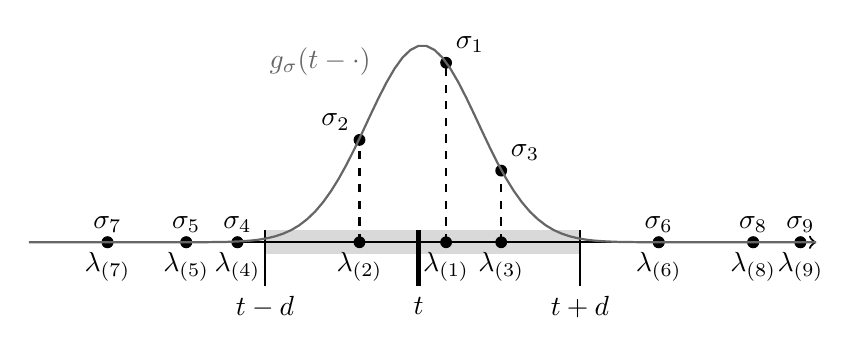
\begin{tikzpicture}
    \fill[black!15!white] (-2.0, -0.15) rectangle (2.0, 0.15);
    \draw[thick, ->] (-5, 0) to (5, 0);
    \fill[black] (-4, 0) circle (0.075) node[below] {$\lambda_{(7)}$};
    \fill[black] (-3, 0) circle (0.075) node[below] {$\lambda_{(5)}$};
    \fill[black] (-2.35, 0) circle (0.075) node[below] {$\lambda_{(4)}$};
    \fill[black] (-0.8, 0) circle (0.075) node[below] {$\lambda_{(2)}$};
    \fill[black] (0.3, 0) circle (0.075) node[below] {$\lambda_{(1)}$};
    \fill[black] (1, 0) circle (0.075) node[below] {$\lambda_{(3)}$};
    \fill[black] (3, 0) circle (0.075) node[below] {$\lambda_{(6)}$};
    \fill[black] (4.2, 0) circle (0.075) node[below] {$\lambda_{(8)}$};
    \fill[black] (4.8, 0) circle (0.075) node[below] {$\lambda_{(9)}$};
    \fill[black] (-4, 0) circle (0.075) node[above] {$\sigma_{7}$};
    \fill[black] (-3, 0) circle (0.075) node[above] {$\sigma_{5}$};
    \fill[black] (-2.35, 0) circle (0.075) node[above] {$\sigma_{4}$};
    \fill[black] (-0.8, 1.3) circle (0.075) node[above left] {$\sigma_{2}$};
    \fill[black] (0.3, 2.28) circle (0.075) node[above right] {$\sigma_{1}$};
    \fill[black] (1, 0.91) circle (0.075) node[above right] {$\sigma_{3}$};
    \fill[black] (3, 0) circle (0.075) node[above] {$\sigma_{6}$};
    \fill[black] (4.2, 0) circle (0.075) node[above] {$\sigma_{8}$};
    \fill[black] (4.8, 0) circle (0.075) node[above] {$\sigma_{9}$};
    \draw[black, ultra thick] (-0.05, 0.15) to (-0.05, -0.55) node[below] {$t$};
    \draw[black, thick] (-2.0, 0.15) to (-2.0, -0.55) node[below] {$t - d$};
    \draw[black, thick] (2.0, 0.15) to (2.0, -0.55) node[below] {$t + d$};
    \draw[black, thick, dashed] (-0.8, 0) to (-0.8, 1.3);
    \draw[black, thick, dashed] (0.3, 0) to (0.3, 2.28);
    \draw[black, thick, dashed] (1, 0) to (1, 0.91);
    \draw[black!60!white, thick] (-5.000, 0.000) to (-4.899, 0.000) to (-4.798, 0.000) to (-4.697, 0.000) to (-4.596, 0.000) to (-4.495, 0.000) to (-4.394, 0.000) to (-4.293, 0.000) to (-4.192, 0.000) to (-4.091, 0.000) to (-3.990, 0.000) to (-3.889, 0.000) to (-3.788, 0.000) to (-3.687, 0.000) to (-3.586, 0.000) to (-3.485, 0.000) to (-3.384, 0.000) to (-3.283, 0.000) to (-3.182, 0.000) to (-3.081, 0.000) to (-2.980, 0.000) to (-2.879, 0.001) to (-2.778, 0.001) to (-2.677, 0.002) to (-2.576, 0.003) to (-2.475, 0.005) to (-2.374, 0.009) to (-2.273, 0.014) to (-2.172, 0.022) to (-2.071, 0.034) to (-1.970, 0.052) to (-1.869, 0.076) to (-1.768, 0.110) to (-1.667, 0.155) to (-1.566, 0.215) to (-1.465, 0.293) to (-1.364, 0.389) to (-1.263, 0.508) to (-1.162, 0.649) to (-1.061, 0.812) to (-0.960, 0.995) to (-0.859, 1.196) to (-0.758, 1.408) to (-0.657, 1.625) to (-0.556, 1.836) to (-0.455, 2.033) to (-0.354, 2.206) to (-0.253, 2.346) to (-0.152, 2.443) to (-0.051, 2.494) to (0.051, 2.494) to (0.152, 2.443) to (0.253, 2.346) to (0.354, 2.206) to (0.455, 2.033) to (0.556, 1.836) to (0.657, 1.625) to (0.758, 1.408) to (0.859, 1.196) to (0.960, 0.995) to (1.061, 0.812) to (1.162, 0.649) to (1.263, 0.508) to (1.364, 0.389) to (1.465, 0.293) to (1.566, 0.215) to (1.667, 0.155) to (1.768, 0.110) to (1.869, 0.076) to (1.970, 0.052) to (2.071, 0.034) to (2.172, 0.022) to (2.273, 0.014) to (2.374, 0.009) to (2.475, 0.005) to (2.576, 0.003) to (2.677, 0.002) to (2.778, 0.001) to (2.879, 0.001) to (2.980, 0.000) to (3.081, 0.000) to (3.182, 0.000) to (3.283, 0.000) to (3.384, 0.000) to (3.485, 0.000) to (3.586, 0.000) to (3.687, 0.000) to (3.788, 0.000) to (3.889, 0.000) to (3.990, 0.000) to (4.091, 0.000) to (4.192, 0.000) to (4.293, 0.000) to (4.394, 0.000) to (4.495, 0.000) to (4.596, 0.000) to (4.697, 0.000) to (4.798, 0.000) to (4.899, 0.000) to (5.000, 0.000);
    \node[black!60!white] at (-1.3, 2.3) {$g_{\sigma}(t - \cdot)$};
\end{tikzpicture}

    \caption{The numerical rank of $g_{\sigma}(t\mtx{I}_n - \mtx{A})$ can be
        approximately computed by counting the number of eigenvalues
        $\lambda_{(1)}, \dots, \lambda_{(n)}$ of the matrix $\mtx{A}$ which lie less than
        a constant $d_{\varepsilon, \sigma}$ away from $t$.}
    \label{fig:numerical-rank}
\end{figure}

If we additionally assume the eigenvalues of the matrix $\mtx{A}$ to be evenly distributed within $[a, b]$, that is, in any subinterval of fixed length in $[a, b]$ we can expect to find roughly the same number of eigenvalues, then we can estimate the numerical rank of $g_{\sigma}(t\mtx{I}_n - \mtx{A})$ to be
\begin{equation}
    r_{\varepsilon}(g_{\sigma}(t\mtx{I}_n - \mtx{A})) \lessapprox \frac{2 n}{b - a} \cdot d_{\varepsilon, \sigma}.
    \label{equ:gaussian-kernel-numerical-rank-uniform}
\end{equation}

\todo{Discuss how this informs choice of $n_{\mtx{\Omega}}$.}

\section{Numerical results}
\label{sec:results}

For our first example, we consider the matrix which arises from the second order
finite difference discretization of the Laplace operator $\Delta$ in a potential
field $V$,
\begin{equation}
    \mathcal{A} u(\vct{x}) = - \Delta u(\vct{x}) + V(\vct{x}) u(\vct{x}),
    \label{equ:5-experiments-electronic-hamiltonian}
\end{equation}
for a uniform mesh of size $h=0.6$. The potential $V$ results from a
lattice whose primitive cell is of side-length $L=6$ and in whose center a
potential
\begin{equation}
    \alpha e^{-\sfrac{\lVert \vct{x} \rVert _2^2}{ 2 \beta^2 }}
    \label{equ:5-experiments-gaussian-cell}
\end{equation}
with $\alpha = -4$, $\beta = 2$ is located. The computational domain is chosen
to span $n_c \in \mathbb{N}$ primitive cells in every spatial dimension, hence, yielding
discretization matrices which are growing in size with $n_c$. In our experiments
we consider the three-dimensional case, but for visualization purposes, we
illustrate the potential in \reffig{fig:gaussian-well}
in two dimensions.

\begin{figure}[ht]
    \begin{subfigure}[b]{0.32\columnwidth}
        %% Creator: Matplotlib, PGF backend
%%
%% To include the figure in your LaTeX document, write
%%   \input{<filename>.pgf}
%%
%% Make sure the required packages are loaded in your preamble
%%   \usepackage{pgf}
%%
%% Also ensure that all the required font packages are loaded; for instance,
%% the lmodern package is sometimes necessary when using math font.
%%   \usepackage{lmodern}
%%
%% Figures using additional raster images can only be included by \input if
%% they are in the same directory as the main LaTeX file. For loading figures
%% from other directories you can use the `import` package
%%   \usepackage{import}
%%
%% and then include the figures with
%%   \import{<path to file>}{<filename>.pgf}
%%
%% Matplotlib used the following preamble
%%   \def\mathdefault#1{#1}
%%   \everymath=\expandafter{\the\everymath\displaystyle}
%%   
%%   \ifdefined\pdftexversion\else  % non-pdftex case.
%%     \usepackage{fontspec}
%%     \setmainfont{DejaVuSerif.ttf}[Path=\detokenize{/opt/hostedtoolcache/Python/3.12.5/x64/lib/python3.12/site-packages/matplotlib/mpl-data/fonts/ttf/}]
%%     \setsansfont{DejaVuSans.ttf}[Path=\detokenize{/opt/hostedtoolcache/Python/3.12.5/x64/lib/python3.12/site-packages/matplotlib/mpl-data/fonts/ttf/}]
%%     \setmonofont{DejaVuSansMono.ttf}[Path=\detokenize{/opt/hostedtoolcache/Python/3.12.5/x64/lib/python3.12/site-packages/matplotlib/mpl-data/fonts/ttf/}]
%%   \fi
%%   \makeatletter\@ifpackageloaded{underscore}{}{\usepackage[strings]{underscore}}\makeatother
%%
\begingroup%
\makeatletter%
\begin{pgfpicture}%
\pgfpathrectangle{\pgfpointorigin}{\pgfqpoint{1.969617in}{1.850740in}}%
\pgfusepath{use as bounding box, clip}%
\begin{pgfscope}%
\pgfsetbuttcap%
\pgfsetmiterjoin%
\definecolor{currentfill}{rgb}{1.000000,1.000000,1.000000}%
\pgfsetfillcolor{currentfill}%
\pgfsetlinewidth{0.000000pt}%
\definecolor{currentstroke}{rgb}{1.000000,1.000000,1.000000}%
\pgfsetstrokecolor{currentstroke}%
\pgfsetdash{}{0pt}%
\pgfpathmoveto{\pgfqpoint{0.000000in}{0.000000in}}%
\pgfpathlineto{\pgfqpoint{1.969617in}{0.000000in}}%
\pgfpathlineto{\pgfqpoint{1.969617in}{1.850740in}}%
\pgfpathlineto{\pgfqpoint{0.000000in}{1.850740in}}%
\pgfpathlineto{\pgfqpoint{0.000000in}{0.000000in}}%
\pgfpathclose%
\pgfusepath{fill}%
\end{pgfscope}%
\begin{pgfscope}%
\pgfsetbuttcap%
\pgfsetmiterjoin%
\definecolor{currentfill}{rgb}{1.000000,1.000000,1.000000}%
\pgfsetfillcolor{currentfill}%
\pgfsetlinewidth{0.000000pt}%
\definecolor{currentstroke}{rgb}{0.000000,0.000000,0.000000}%
\pgfsetstrokecolor{currentstroke}%
\pgfsetstrokeopacity{0.000000}%
\pgfsetdash{}{0pt}%
\pgfpathmoveto{\pgfqpoint{0.278819in}{0.345370in}}%
\pgfpathlineto{\pgfqpoint{1.828819in}{0.345370in}}%
\pgfpathlineto{\pgfqpoint{1.828819in}{1.692870in}}%
\pgfpathlineto{\pgfqpoint{0.278819in}{1.692870in}}%
\pgfpathlineto{\pgfqpoint{0.278819in}{0.345370in}}%
\pgfpathclose%
\pgfusepath{fill}%
\end{pgfscope}%
\begin{pgfscope}%
\pgfpathrectangle{\pgfqpoint{0.278819in}{0.345370in}}{\pgfqpoint{1.550000in}{1.347500in}}%
\pgfusepath{clip}%
\pgfsetbuttcap%
\pgfsetroundjoin%
\definecolor{currentfill}{rgb}{0.972530,0.881250,0.144923}%
\pgfsetfillcolor{currentfill}%
\pgfsetlinewidth{0.000000pt}%
\definecolor{currentstroke}{rgb}{0.000000,0.000000,0.000000}%
\pgfsetstrokecolor{currentstroke}%
\pgfsetdash{}{0pt}%
\pgfpathmoveto{\pgfqpoint{1.014677in}{0.833047in}}%
\pgfpathlineto{\pgfqpoint{1.030334in}{0.830965in}}%
\pgfpathlineto{\pgfqpoint{1.045990in}{0.829924in}}%
\pgfpathlineto{\pgfqpoint{1.061647in}{0.829924in}}%
\pgfpathlineto{\pgfqpoint{1.077303in}{0.830965in}}%
\pgfpathlineto{\pgfqpoint{1.092960in}{0.833047in}}%
\pgfpathlineto{\pgfqpoint{1.104609in}{0.835370in}}%
\pgfpathlineto{\pgfqpoint{1.108617in}{0.836216in}}%
\pgfpathlineto{\pgfqpoint{1.124273in}{0.840617in}}%
\pgfpathlineto{\pgfqpoint{1.139930in}{0.846121in}}%
\pgfpathlineto{\pgfqpoint{1.146722in}{0.848981in}}%
\pgfpathlineto{\pgfqpoint{1.155586in}{0.852970in}}%
\pgfpathlineto{\pgfqpoint{1.171243in}{0.861179in}}%
\pgfpathlineto{\pgfqpoint{1.173612in}{0.862592in}}%
\pgfpathlineto{\pgfqpoint{1.186899in}{0.871149in}}%
\pgfpathlineto{\pgfqpoint{1.193903in}{0.876203in}}%
\pgfpathlineto{\pgfqpoint{1.202556in}{0.883015in}}%
\pgfpathlineto{\pgfqpoint{1.210377in}{0.889814in}}%
\pgfpathlineto{\pgfqpoint{1.218213in}{0.897337in}}%
\pgfpathlineto{\pgfqpoint{1.224026in}{0.903425in}}%
\pgfpathlineto{\pgfqpoint{1.233869in}{0.914977in}}%
\pgfpathlineto{\pgfqpoint{1.235495in}{0.917036in}}%
\pgfpathlineto{\pgfqpoint{1.244937in}{0.930648in}}%
\pgfpathlineto{\pgfqpoint{1.249526in}{0.938354in}}%
\pgfpathlineto{\pgfqpoint{1.252815in}{0.944259in}}%
\pgfpathlineto{\pgfqpoint{1.259146in}{0.957870in}}%
\pgfpathlineto{\pgfqpoint{1.264209in}{0.971481in}}%
\pgfpathlineto{\pgfqpoint{1.265182in}{0.974965in}}%
\pgfpathlineto{\pgfqpoint{1.267854in}{0.985092in}}%
\pgfpathlineto{\pgfqpoint{1.270249in}{0.998703in}}%
\pgfpathlineto{\pgfqpoint{1.271447in}{1.012314in}}%
\pgfpathlineto{\pgfqpoint{1.271447in}{1.025925in}}%
\pgfpathlineto{\pgfqpoint{1.270249in}{1.039536in}}%
\pgfpathlineto{\pgfqpoint{1.267854in}{1.053148in}}%
\pgfpathlineto{\pgfqpoint{1.265182in}{1.063275in}}%
\pgfpathlineto{\pgfqpoint{1.264209in}{1.066759in}}%
\pgfpathlineto{\pgfqpoint{1.259146in}{1.080370in}}%
\pgfpathlineto{\pgfqpoint{1.252815in}{1.093981in}}%
\pgfpathlineto{\pgfqpoint{1.249526in}{1.099886in}}%
\pgfpathlineto{\pgfqpoint{1.244937in}{1.107592in}}%
\pgfpathlineto{\pgfqpoint{1.235495in}{1.121203in}}%
\pgfpathlineto{\pgfqpoint{1.233869in}{1.123262in}}%
\pgfpathlineto{\pgfqpoint{1.224026in}{1.134814in}}%
\pgfpathlineto{\pgfqpoint{1.218213in}{1.140902in}}%
\pgfpathlineto{\pgfqpoint{1.210377in}{1.148425in}}%
\pgfpathlineto{\pgfqpoint{1.202556in}{1.155224in}}%
\pgfpathlineto{\pgfqpoint{1.193903in}{1.162036in}}%
\pgfpathlineto{\pgfqpoint{1.186899in}{1.167090in}}%
\pgfpathlineto{\pgfqpoint{1.173612in}{1.175647in}}%
\pgfpathlineto{\pgfqpoint{1.171243in}{1.177061in}}%
\pgfpathlineto{\pgfqpoint{1.155586in}{1.185269in}}%
\pgfpathlineto{\pgfqpoint{1.146722in}{1.189259in}}%
\pgfpathlineto{\pgfqpoint{1.139930in}{1.192118in}}%
\pgfpathlineto{\pgfqpoint{1.124273in}{1.197622in}}%
\pgfpathlineto{\pgfqpoint{1.108617in}{1.202024in}}%
\pgfpathlineto{\pgfqpoint{1.104609in}{1.202870in}}%
\pgfpathlineto{\pgfqpoint{1.092960in}{1.205193in}}%
\pgfpathlineto{\pgfqpoint{1.077303in}{1.207275in}}%
\pgfpathlineto{\pgfqpoint{1.061647in}{1.208316in}}%
\pgfpathlineto{\pgfqpoint{1.045990in}{1.208316in}}%
\pgfpathlineto{\pgfqpoint{1.030334in}{1.207275in}}%
\pgfpathlineto{\pgfqpoint{1.014677in}{1.205193in}}%
\pgfpathlineto{\pgfqpoint{1.003028in}{1.202870in}}%
\pgfpathlineto{\pgfqpoint{0.999021in}{1.202024in}}%
\pgfpathlineto{\pgfqpoint{0.983364in}{1.197622in}}%
\pgfpathlineto{\pgfqpoint{0.967708in}{1.192118in}}%
\pgfpathlineto{\pgfqpoint{0.960915in}{1.189259in}}%
\pgfpathlineto{\pgfqpoint{0.952051in}{1.185269in}}%
\pgfpathlineto{\pgfqpoint{0.936394in}{1.177061in}}%
\pgfpathlineto{\pgfqpoint{0.934026in}{1.175647in}}%
\pgfpathlineto{\pgfqpoint{0.920738in}{1.167090in}}%
\pgfpathlineto{\pgfqpoint{0.913735in}{1.162036in}}%
\pgfpathlineto{\pgfqpoint{0.905081in}{1.155224in}}%
\pgfpathlineto{\pgfqpoint{0.897261in}{1.148425in}}%
\pgfpathlineto{\pgfqpoint{0.889425in}{1.140902in}}%
\pgfpathlineto{\pgfqpoint{0.883612in}{1.134814in}}%
\pgfpathlineto{\pgfqpoint{0.873768in}{1.123262in}}%
\pgfpathlineto{\pgfqpoint{0.872143in}{1.121203in}}%
\pgfpathlineto{\pgfqpoint{0.862700in}{1.107592in}}%
\pgfpathlineto{\pgfqpoint{0.858112in}{1.099886in}}%
\pgfpathlineto{\pgfqpoint{0.854822in}{1.093981in}}%
\pgfpathlineto{\pgfqpoint{0.848491in}{1.080370in}}%
\pgfpathlineto{\pgfqpoint{0.843428in}{1.066759in}}%
\pgfpathlineto{\pgfqpoint{0.842455in}{1.063275in}}%
\pgfpathlineto{\pgfqpoint{0.839783in}{1.053147in}}%
\pgfpathlineto{\pgfqpoint{0.837388in}{1.039536in}}%
\pgfpathlineto{\pgfqpoint{0.836190in}{1.025925in}}%
\pgfpathlineto{\pgfqpoint{0.836190in}{1.012314in}}%
\pgfpathlineto{\pgfqpoint{0.837388in}{0.998703in}}%
\pgfpathlineto{\pgfqpoint{0.839783in}{0.985092in}}%
\pgfpathlineto{\pgfqpoint{0.842455in}{0.974965in}}%
\pgfpathlineto{\pgfqpoint{0.843428in}{0.971481in}}%
\pgfpathlineto{\pgfqpoint{0.848491in}{0.957870in}}%
\pgfpathlineto{\pgfqpoint{0.854822in}{0.944259in}}%
\pgfpathlineto{\pgfqpoint{0.858112in}{0.938354in}}%
\pgfpathlineto{\pgfqpoint{0.862700in}{0.930648in}}%
\pgfpathlineto{\pgfqpoint{0.872143in}{0.917036in}}%
\pgfpathlineto{\pgfqpoint{0.873768in}{0.914977in}}%
\pgfpathlineto{\pgfqpoint{0.883612in}{0.903425in}}%
\pgfpathlineto{\pgfqpoint{0.889425in}{0.897337in}}%
\pgfpathlineto{\pgfqpoint{0.897261in}{0.889814in}}%
\pgfpathlineto{\pgfqpoint{0.905081in}{0.883015in}}%
\pgfpathlineto{\pgfqpoint{0.913735in}{0.876203in}}%
\pgfpathlineto{\pgfqpoint{0.920738in}{0.871149in}}%
\pgfpathlineto{\pgfqpoint{0.934026in}{0.862592in}}%
\pgfpathlineto{\pgfqpoint{0.936394in}{0.861179in}}%
\pgfpathlineto{\pgfqpoint{0.952051in}{0.852970in}}%
\pgfpathlineto{\pgfqpoint{0.960915in}{0.848981in}}%
\pgfpathlineto{\pgfqpoint{0.967708in}{0.846121in}}%
\pgfpathlineto{\pgfqpoint{0.983364in}{0.840617in}}%
\pgfpathlineto{\pgfqpoint{0.999021in}{0.836216in}}%
\pgfpathlineto{\pgfqpoint{1.003028in}{0.835370in}}%
\pgfpathlineto{\pgfqpoint{1.014677in}{0.833047in}}%
\pgfpathclose%
\pgfusepath{fill}%
\end{pgfscope}%
\begin{pgfscope}%
\pgfpathrectangle{\pgfqpoint{0.278819in}{0.345370in}}{\pgfqpoint{1.550000in}{1.347500in}}%
\pgfusepath{clip}%
\pgfsetbuttcap%
\pgfsetroundjoin%
\definecolor{currentfill}{rgb}{0.993814,0.704741,0.183043}%
\pgfsetfillcolor{currentfill}%
\pgfsetlinewidth{0.000000pt}%
\definecolor{currentstroke}{rgb}{0.000000,0.000000,0.000000}%
\pgfsetstrokecolor{currentstroke}%
\pgfsetdash{}{0pt}%
\pgfpathmoveto{\pgfqpoint{0.999021in}{0.739415in}}%
\pgfpathlineto{\pgfqpoint{1.014677in}{0.737106in}}%
\pgfpathlineto{\pgfqpoint{1.030334in}{0.735568in}}%
\pgfpathlineto{\pgfqpoint{1.045990in}{0.734799in}}%
\pgfpathlineto{\pgfqpoint{1.061647in}{0.734799in}}%
\pgfpathlineto{\pgfqpoint{1.077303in}{0.735568in}}%
\pgfpathlineto{\pgfqpoint{1.092960in}{0.737106in}}%
\pgfpathlineto{\pgfqpoint{1.108617in}{0.739415in}}%
\pgfpathlineto{\pgfqpoint{1.112069in}{0.740092in}}%
\pgfpathlineto{\pgfqpoint{1.124273in}{0.742535in}}%
\pgfpathlineto{\pgfqpoint{1.139930in}{0.746452in}}%
\pgfpathlineto{\pgfqpoint{1.155586in}{0.751154in}}%
\pgfpathlineto{\pgfqpoint{1.162877in}{0.753703in}}%
\pgfpathlineto{\pgfqpoint{1.171243in}{0.756707in}}%
\pgfpathlineto{\pgfqpoint{1.186899in}{0.763121in}}%
\pgfpathlineto{\pgfqpoint{1.196020in}{0.767314in}}%
\pgfpathlineto{\pgfqpoint{1.202556in}{0.770419in}}%
\pgfpathlineto{\pgfqpoint{1.218213in}{0.778656in}}%
\pgfpathlineto{\pgfqpoint{1.222157in}{0.780925in}}%
\pgfpathlineto{\pgfqpoint{1.233869in}{0.787933in}}%
\pgfpathlineto{\pgfqpoint{1.244037in}{0.794536in}}%
\pgfpathlineto{\pgfqpoint{1.249526in}{0.798265in}}%
\pgfpathlineto{\pgfqpoint{1.263051in}{0.808148in}}%
\pgfpathlineto{\pgfqpoint{1.265182in}{0.809786in}}%
\pgfpathlineto{\pgfqpoint{1.279772in}{0.821759in}}%
\pgfpathlineto{\pgfqpoint{1.280839in}{0.822686in}}%
\pgfpathlineto{\pgfqpoint{1.294610in}{0.835370in}}%
\pgfpathlineto{\pgfqpoint{1.296495in}{0.837223in}}%
\pgfpathlineto{\pgfqpoint{1.307864in}{0.848981in}}%
\pgfpathlineto{\pgfqpoint{1.312152in}{0.853753in}}%
\pgfpathlineto{\pgfqpoint{1.319748in}{0.862592in}}%
\pgfpathlineto{\pgfqpoint{1.327809in}{0.872774in}}%
\pgfpathlineto{\pgfqpoint{1.330419in}{0.876203in}}%
\pgfpathlineto{\pgfqpoint{1.339893in}{0.889814in}}%
\pgfpathlineto{\pgfqpoint{1.343465in}{0.895496in}}%
\pgfpathlineto{\pgfqpoint{1.348289in}{0.903425in}}%
\pgfpathlineto{\pgfqpoint{1.355666in}{0.917036in}}%
\pgfpathlineto{\pgfqpoint{1.359122in}{0.924309in}}%
\pgfpathlineto{\pgfqpoint{1.362054in}{0.930648in}}%
\pgfpathlineto{\pgfqpoint{1.367463in}{0.944259in}}%
\pgfpathlineto{\pgfqpoint{1.371968in}{0.957870in}}%
\pgfpathlineto{\pgfqpoint{1.374778in}{0.968479in}}%
\pgfpathlineto{\pgfqpoint{1.375557in}{0.971481in}}%
\pgfpathlineto{\pgfqpoint{1.378212in}{0.985092in}}%
\pgfpathlineto{\pgfqpoint{1.379982in}{0.998703in}}%
\pgfpathlineto{\pgfqpoint{1.380866in}{1.012314in}}%
\pgfpathlineto{\pgfqpoint{1.380866in}{1.025925in}}%
\pgfpathlineto{\pgfqpoint{1.379982in}{1.039536in}}%
\pgfpathlineto{\pgfqpoint{1.378212in}{1.053148in}}%
\pgfpathlineto{\pgfqpoint{1.375557in}{1.066759in}}%
\pgfpathlineto{\pgfqpoint{1.374778in}{1.069760in}}%
\pgfpathlineto{\pgfqpoint{1.371968in}{1.080370in}}%
\pgfpathlineto{\pgfqpoint{1.367463in}{1.093981in}}%
\pgfpathlineto{\pgfqpoint{1.362054in}{1.107592in}}%
\pgfpathlineto{\pgfqpoint{1.359122in}{1.113930in}}%
\pgfpathlineto{\pgfqpoint{1.355666in}{1.121203in}}%
\pgfpathlineto{\pgfqpoint{1.348289in}{1.134814in}}%
\pgfpathlineto{\pgfqpoint{1.343465in}{1.142743in}}%
\pgfpathlineto{\pgfqpoint{1.339893in}{1.148425in}}%
\pgfpathlineto{\pgfqpoint{1.330419in}{1.162036in}}%
\pgfpathlineto{\pgfqpoint{1.327809in}{1.165465in}}%
\pgfpathlineto{\pgfqpoint{1.319748in}{1.175647in}}%
\pgfpathlineto{\pgfqpoint{1.312152in}{1.184487in}}%
\pgfpathlineto{\pgfqpoint{1.307864in}{1.189259in}}%
\pgfpathlineto{\pgfqpoint{1.296495in}{1.201017in}}%
\pgfpathlineto{\pgfqpoint{1.294610in}{1.202870in}}%
\pgfpathlineto{\pgfqpoint{1.280839in}{1.215553in}}%
\pgfpathlineto{\pgfqpoint{1.279772in}{1.216481in}}%
\pgfpathlineto{\pgfqpoint{1.265182in}{1.228453in}}%
\pgfpathlineto{\pgfqpoint{1.263051in}{1.230092in}}%
\pgfpathlineto{\pgfqpoint{1.249526in}{1.239975in}}%
\pgfpathlineto{\pgfqpoint{1.244037in}{1.243703in}}%
\pgfpathlineto{\pgfqpoint{1.233869in}{1.250307in}}%
\pgfpathlineto{\pgfqpoint{1.222157in}{1.257314in}}%
\pgfpathlineto{\pgfqpoint{1.218213in}{1.259584in}}%
\pgfpathlineto{\pgfqpoint{1.202556in}{1.267820in}}%
\pgfpathlineto{\pgfqpoint{1.196020in}{1.270925in}}%
\pgfpathlineto{\pgfqpoint{1.186899in}{1.275119in}}%
\pgfpathlineto{\pgfqpoint{1.171243in}{1.281532in}}%
\pgfpathlineto{\pgfqpoint{1.162877in}{1.284536in}}%
\pgfpathlineto{\pgfqpoint{1.155586in}{1.287085in}}%
\pgfpathlineto{\pgfqpoint{1.139930in}{1.291788in}}%
\pgfpathlineto{\pgfqpoint{1.124273in}{1.295705in}}%
\pgfpathlineto{\pgfqpoint{1.112069in}{1.298148in}}%
\pgfpathlineto{\pgfqpoint{1.108617in}{1.298825in}}%
\pgfpathlineto{\pgfqpoint{1.092960in}{1.301133in}}%
\pgfpathlineto{\pgfqpoint{1.077303in}{1.302671in}}%
\pgfpathlineto{\pgfqpoint{1.061647in}{1.303440in}}%
\pgfpathlineto{\pgfqpoint{1.045990in}{1.303440in}}%
\pgfpathlineto{\pgfqpoint{1.030334in}{1.302671in}}%
\pgfpathlineto{\pgfqpoint{1.014677in}{1.301133in}}%
\pgfpathlineto{\pgfqpoint{0.999021in}{1.298825in}}%
\pgfpathlineto{\pgfqpoint{0.995568in}{1.298148in}}%
\pgfpathlineto{\pgfqpoint{0.983364in}{1.295705in}}%
\pgfpathlineto{\pgfqpoint{0.967708in}{1.291788in}}%
\pgfpathlineto{\pgfqpoint{0.952051in}{1.287085in}}%
\pgfpathlineto{\pgfqpoint{0.944760in}{1.284536in}}%
\pgfpathlineto{\pgfqpoint{0.936394in}{1.281532in}}%
\pgfpathlineto{\pgfqpoint{0.920738in}{1.275119in}}%
\pgfpathlineto{\pgfqpoint{0.911617in}{1.270925in}}%
\pgfpathlineto{\pgfqpoint{0.905081in}{1.267820in}}%
\pgfpathlineto{\pgfqpoint{0.889425in}{1.259584in}}%
\pgfpathlineto{\pgfqpoint{0.885481in}{1.257314in}}%
\pgfpathlineto{\pgfqpoint{0.873768in}{1.250307in}}%
\pgfpathlineto{\pgfqpoint{0.863600in}{1.243703in}}%
\pgfpathlineto{\pgfqpoint{0.858112in}{1.239975in}}%
\pgfpathlineto{\pgfqpoint{0.844586in}{1.230092in}}%
\pgfpathlineto{\pgfqpoint{0.842455in}{1.228453in}}%
\pgfpathlineto{\pgfqpoint{0.827865in}{1.216481in}}%
\pgfpathlineto{\pgfqpoint{0.826798in}{1.215553in}}%
\pgfpathlineto{\pgfqpoint{0.813027in}{1.202870in}}%
\pgfpathlineto{\pgfqpoint{0.811142in}{1.201017in}}%
\pgfpathlineto{\pgfqpoint{0.799774in}{1.189259in}}%
\pgfpathlineto{\pgfqpoint{0.795485in}{1.184487in}}%
\pgfpathlineto{\pgfqpoint{0.787889in}{1.175647in}}%
\pgfpathlineto{\pgfqpoint{0.779829in}{1.165465in}}%
\pgfpathlineto{\pgfqpoint{0.777218in}{1.162036in}}%
\pgfpathlineto{\pgfqpoint{0.767744in}{1.148425in}}%
\pgfpathlineto{\pgfqpoint{0.764172in}{1.142743in}}%
\pgfpathlineto{\pgfqpoint{0.759348in}{1.134814in}}%
\pgfpathlineto{\pgfqpoint{0.751971in}{1.121203in}}%
\pgfpathlineto{\pgfqpoint{0.748516in}{1.113930in}}%
\pgfpathlineto{\pgfqpoint{0.745583in}{1.107592in}}%
\pgfpathlineto{\pgfqpoint{0.740174in}{1.093981in}}%
\pgfpathlineto{\pgfqpoint{0.735669in}{1.080370in}}%
\pgfpathlineto{\pgfqpoint{0.732859in}{1.069760in}}%
\pgfpathlineto{\pgfqpoint{0.732080in}{1.066759in}}%
\pgfpathlineto{\pgfqpoint{0.729425in}{1.053148in}}%
\pgfpathlineto{\pgfqpoint{0.727655in}{1.039536in}}%
\pgfpathlineto{\pgfqpoint{0.726771in}{1.025925in}}%
\pgfpathlineto{\pgfqpoint{0.726771in}{1.012314in}}%
\pgfpathlineto{\pgfqpoint{0.727655in}{0.998703in}}%
\pgfpathlineto{\pgfqpoint{0.729425in}{0.985092in}}%
\pgfpathlineto{\pgfqpoint{0.732080in}{0.971481in}}%
\pgfpathlineto{\pgfqpoint{0.732859in}{0.968479in}}%
\pgfpathlineto{\pgfqpoint{0.735669in}{0.957870in}}%
\pgfpathlineto{\pgfqpoint{0.740174in}{0.944259in}}%
\pgfpathlineto{\pgfqpoint{0.745583in}{0.930648in}}%
\pgfpathlineto{\pgfqpoint{0.748516in}{0.924309in}}%
\pgfpathlineto{\pgfqpoint{0.751971in}{0.917036in}}%
\pgfpathlineto{\pgfqpoint{0.759348in}{0.903425in}}%
\pgfpathlineto{\pgfqpoint{0.764172in}{0.895496in}}%
\pgfpathlineto{\pgfqpoint{0.767744in}{0.889814in}}%
\pgfpathlineto{\pgfqpoint{0.777218in}{0.876203in}}%
\pgfpathlineto{\pgfqpoint{0.779829in}{0.872774in}}%
\pgfpathlineto{\pgfqpoint{0.787889in}{0.862592in}}%
\pgfpathlineto{\pgfqpoint{0.795485in}{0.853753in}}%
\pgfpathlineto{\pgfqpoint{0.799774in}{0.848981in}}%
\pgfpathlineto{\pgfqpoint{0.811142in}{0.837223in}}%
\pgfpathlineto{\pgfqpoint{0.813027in}{0.835370in}}%
\pgfpathlineto{\pgfqpoint{0.826798in}{0.822686in}}%
\pgfpathlineto{\pgfqpoint{0.827865in}{0.821759in}}%
\pgfpathlineto{\pgfqpoint{0.842455in}{0.809786in}}%
\pgfpathlineto{\pgfqpoint{0.844586in}{0.808148in}}%
\pgfpathlineto{\pgfqpoint{0.858112in}{0.798265in}}%
\pgfpathlineto{\pgfqpoint{0.863600in}{0.794536in}}%
\pgfpathlineto{\pgfqpoint{0.873768in}{0.787933in}}%
\pgfpathlineto{\pgfqpoint{0.885481in}{0.780925in}}%
\pgfpathlineto{\pgfqpoint{0.889425in}{0.778656in}}%
\pgfpathlineto{\pgfqpoint{0.905081in}{0.770419in}}%
\pgfpathlineto{\pgfqpoint{0.911617in}{0.767314in}}%
\pgfpathlineto{\pgfqpoint{0.920738in}{0.763121in}}%
\pgfpathlineto{\pgfqpoint{0.936394in}{0.756707in}}%
\pgfpathlineto{\pgfqpoint{0.944760in}{0.753703in}}%
\pgfpathlineto{\pgfqpoint{0.952051in}{0.751154in}}%
\pgfpathlineto{\pgfqpoint{0.967708in}{0.746452in}}%
\pgfpathlineto{\pgfqpoint{0.983364in}{0.742535in}}%
\pgfpathlineto{\pgfqpoint{0.995568in}{0.740092in}}%
\pgfpathlineto{\pgfqpoint{0.999021in}{0.739415in}}%
\pgfpathclose%
\pgfpathmoveto{\pgfqpoint{1.003028in}{0.835370in}}%
\pgfpathlineto{\pgfqpoint{0.999021in}{0.836216in}}%
\pgfpathlineto{\pgfqpoint{0.983364in}{0.840617in}}%
\pgfpathlineto{\pgfqpoint{0.967708in}{0.846121in}}%
\pgfpathlineto{\pgfqpoint{0.960915in}{0.848981in}}%
\pgfpathlineto{\pgfqpoint{0.952051in}{0.852970in}}%
\pgfpathlineto{\pgfqpoint{0.936394in}{0.861179in}}%
\pgfpathlineto{\pgfqpoint{0.934026in}{0.862592in}}%
\pgfpathlineto{\pgfqpoint{0.920738in}{0.871149in}}%
\pgfpathlineto{\pgfqpoint{0.913735in}{0.876203in}}%
\pgfpathlineto{\pgfqpoint{0.905081in}{0.883015in}}%
\pgfpathlineto{\pgfqpoint{0.897261in}{0.889814in}}%
\pgfpathlineto{\pgfqpoint{0.889425in}{0.897337in}}%
\pgfpathlineto{\pgfqpoint{0.883612in}{0.903425in}}%
\pgfpathlineto{\pgfqpoint{0.873768in}{0.914977in}}%
\pgfpathlineto{\pgfqpoint{0.872143in}{0.917036in}}%
\pgfpathlineto{\pgfqpoint{0.862700in}{0.930648in}}%
\pgfpathlineto{\pgfqpoint{0.858112in}{0.938354in}}%
\pgfpathlineto{\pgfqpoint{0.854822in}{0.944259in}}%
\pgfpathlineto{\pgfqpoint{0.848491in}{0.957870in}}%
\pgfpathlineto{\pgfqpoint{0.843428in}{0.971481in}}%
\pgfpathlineto{\pgfqpoint{0.842455in}{0.974965in}}%
\pgfpathlineto{\pgfqpoint{0.839783in}{0.985092in}}%
\pgfpathlineto{\pgfqpoint{0.837388in}{0.998703in}}%
\pgfpathlineto{\pgfqpoint{0.836190in}{1.012314in}}%
\pgfpathlineto{\pgfqpoint{0.836190in}{1.025925in}}%
\pgfpathlineto{\pgfqpoint{0.837388in}{1.039536in}}%
\pgfpathlineto{\pgfqpoint{0.839783in}{1.053148in}}%
\pgfpathlineto{\pgfqpoint{0.842455in}{1.063275in}}%
\pgfpathlineto{\pgfqpoint{0.843428in}{1.066759in}}%
\pgfpathlineto{\pgfqpoint{0.848491in}{1.080370in}}%
\pgfpathlineto{\pgfqpoint{0.854822in}{1.093981in}}%
\pgfpathlineto{\pgfqpoint{0.858112in}{1.099886in}}%
\pgfpathlineto{\pgfqpoint{0.862700in}{1.107592in}}%
\pgfpathlineto{\pgfqpoint{0.872143in}{1.121203in}}%
\pgfpathlineto{\pgfqpoint{0.873768in}{1.123262in}}%
\pgfpathlineto{\pgfqpoint{0.883612in}{1.134814in}}%
\pgfpathlineto{\pgfqpoint{0.889425in}{1.140902in}}%
\pgfpathlineto{\pgfqpoint{0.897261in}{1.148425in}}%
\pgfpathlineto{\pgfqpoint{0.905081in}{1.155224in}}%
\pgfpathlineto{\pgfqpoint{0.913735in}{1.162036in}}%
\pgfpathlineto{\pgfqpoint{0.920738in}{1.167090in}}%
\pgfpathlineto{\pgfqpoint{0.934026in}{1.175647in}}%
\pgfpathlineto{\pgfqpoint{0.936394in}{1.177061in}}%
\pgfpathlineto{\pgfqpoint{0.952051in}{1.185269in}}%
\pgfpathlineto{\pgfqpoint{0.960915in}{1.189259in}}%
\pgfpathlineto{\pgfqpoint{0.967708in}{1.192118in}}%
\pgfpathlineto{\pgfqpoint{0.983364in}{1.197622in}}%
\pgfpathlineto{\pgfqpoint{0.999021in}{1.202024in}}%
\pgfpathlineto{\pgfqpoint{1.003028in}{1.202870in}}%
\pgfpathlineto{\pgfqpoint{1.014677in}{1.205193in}}%
\pgfpathlineto{\pgfqpoint{1.030334in}{1.207275in}}%
\pgfpathlineto{\pgfqpoint{1.045990in}{1.208316in}}%
\pgfpathlineto{\pgfqpoint{1.061647in}{1.208316in}}%
\pgfpathlineto{\pgfqpoint{1.077303in}{1.207275in}}%
\pgfpathlineto{\pgfqpoint{1.092960in}{1.205193in}}%
\pgfpathlineto{\pgfqpoint{1.104609in}{1.202870in}}%
\pgfpathlineto{\pgfqpoint{1.108617in}{1.202024in}}%
\pgfpathlineto{\pgfqpoint{1.124273in}{1.197622in}}%
\pgfpathlineto{\pgfqpoint{1.139930in}{1.192118in}}%
\pgfpathlineto{\pgfqpoint{1.146722in}{1.189259in}}%
\pgfpathlineto{\pgfqpoint{1.155586in}{1.185269in}}%
\pgfpathlineto{\pgfqpoint{1.171243in}{1.177061in}}%
\pgfpathlineto{\pgfqpoint{1.173612in}{1.175647in}}%
\pgfpathlineto{\pgfqpoint{1.186899in}{1.167090in}}%
\pgfpathlineto{\pgfqpoint{1.193903in}{1.162036in}}%
\pgfpathlineto{\pgfqpoint{1.202556in}{1.155224in}}%
\pgfpathlineto{\pgfqpoint{1.210377in}{1.148425in}}%
\pgfpathlineto{\pgfqpoint{1.218213in}{1.140902in}}%
\pgfpathlineto{\pgfqpoint{1.224026in}{1.134814in}}%
\pgfpathlineto{\pgfqpoint{1.233869in}{1.123262in}}%
\pgfpathlineto{\pgfqpoint{1.235495in}{1.121203in}}%
\pgfpathlineto{\pgfqpoint{1.244937in}{1.107592in}}%
\pgfpathlineto{\pgfqpoint{1.249526in}{1.099886in}}%
\pgfpathlineto{\pgfqpoint{1.252815in}{1.093981in}}%
\pgfpathlineto{\pgfqpoint{1.259146in}{1.080370in}}%
\pgfpathlineto{\pgfqpoint{1.264209in}{1.066759in}}%
\pgfpathlineto{\pgfqpoint{1.265182in}{1.063275in}}%
\pgfpathlineto{\pgfqpoint{1.267854in}{1.053148in}}%
\pgfpathlineto{\pgfqpoint{1.270249in}{1.039536in}}%
\pgfpathlineto{\pgfqpoint{1.271447in}{1.025925in}}%
\pgfpathlineto{\pgfqpoint{1.271447in}{1.012314in}}%
\pgfpathlineto{\pgfqpoint{1.270249in}{0.998703in}}%
\pgfpathlineto{\pgfqpoint{1.267854in}{0.985092in}}%
\pgfpathlineto{\pgfqpoint{1.265182in}{0.974965in}}%
\pgfpathlineto{\pgfqpoint{1.264209in}{0.971481in}}%
\pgfpathlineto{\pgfqpoint{1.259146in}{0.957870in}}%
\pgfpathlineto{\pgfqpoint{1.252815in}{0.944259in}}%
\pgfpathlineto{\pgfqpoint{1.249526in}{0.938354in}}%
\pgfpathlineto{\pgfqpoint{1.244937in}{0.930648in}}%
\pgfpathlineto{\pgfqpoint{1.235495in}{0.917036in}}%
\pgfpathlineto{\pgfqpoint{1.233869in}{0.914977in}}%
\pgfpathlineto{\pgfqpoint{1.224026in}{0.903425in}}%
\pgfpathlineto{\pgfqpoint{1.218213in}{0.897337in}}%
\pgfpathlineto{\pgfqpoint{1.210377in}{0.889814in}}%
\pgfpathlineto{\pgfqpoint{1.202556in}{0.883015in}}%
\pgfpathlineto{\pgfqpoint{1.193903in}{0.876203in}}%
\pgfpathlineto{\pgfqpoint{1.186899in}{0.871149in}}%
\pgfpathlineto{\pgfqpoint{1.173612in}{0.862592in}}%
\pgfpathlineto{\pgfqpoint{1.171243in}{0.861179in}}%
\pgfpathlineto{\pgfqpoint{1.155586in}{0.852970in}}%
\pgfpathlineto{\pgfqpoint{1.146722in}{0.848981in}}%
\pgfpathlineto{\pgfqpoint{1.139930in}{0.846121in}}%
\pgfpathlineto{\pgfqpoint{1.124273in}{0.840617in}}%
\pgfpathlineto{\pgfqpoint{1.108617in}{0.836216in}}%
\pgfpathlineto{\pgfqpoint{1.104609in}{0.835370in}}%
\pgfpathlineto{\pgfqpoint{1.092960in}{0.833047in}}%
\pgfpathlineto{\pgfqpoint{1.077303in}{0.830965in}}%
\pgfpathlineto{\pgfqpoint{1.061647in}{0.829924in}}%
\pgfpathlineto{\pgfqpoint{1.045990in}{0.829924in}}%
\pgfpathlineto{\pgfqpoint{1.030334in}{0.830965in}}%
\pgfpathlineto{\pgfqpoint{1.014677in}{0.833047in}}%
\pgfpathlineto{\pgfqpoint{1.003028in}{0.835370in}}%
\pgfpathclose%
\pgfusepath{fill}%
\end{pgfscope}%
\begin{pgfscope}%
\pgfpathrectangle{\pgfqpoint{0.278819in}{0.345370in}}{\pgfqpoint{1.550000in}{1.347500in}}%
\pgfusepath{clip}%
\pgfsetbuttcap%
\pgfsetroundjoin%
\definecolor{currentfill}{rgb}{0.959424,0.543431,0.278701}%
\pgfsetfillcolor{currentfill}%
\pgfsetlinewidth{0.000000pt}%
\definecolor{currentstroke}{rgb}{0.000000,0.000000,0.000000}%
\pgfsetstrokecolor{currentstroke}%
\pgfsetdash{}{0pt}%
\pgfpathmoveto{\pgfqpoint{0.983364in}{0.656656in}}%
\pgfpathlineto{\pgfqpoint{0.999021in}{0.653880in}}%
\pgfpathlineto{\pgfqpoint{1.014677in}{0.651798in}}%
\pgfpathlineto{\pgfqpoint{1.030334in}{0.650411in}}%
\pgfpathlineto{\pgfqpoint{1.045990in}{0.649717in}}%
\pgfpathlineto{\pgfqpoint{1.061647in}{0.649717in}}%
\pgfpathlineto{\pgfqpoint{1.077303in}{0.650411in}}%
\pgfpathlineto{\pgfqpoint{1.092960in}{0.651798in}}%
\pgfpathlineto{\pgfqpoint{1.108617in}{0.653880in}}%
\pgfpathlineto{\pgfqpoint{1.124273in}{0.656656in}}%
\pgfpathlineto{\pgfqpoint{1.132264in}{0.658425in}}%
\pgfpathlineto{\pgfqpoint{1.139930in}{0.660116in}}%
\pgfpathlineto{\pgfqpoint{1.155586in}{0.664254in}}%
\pgfpathlineto{\pgfqpoint{1.171243in}{0.669083in}}%
\pgfpathlineto{\pgfqpoint{1.179638in}{0.672036in}}%
\pgfpathlineto{\pgfqpoint{1.186899in}{0.674597in}}%
\pgfpathlineto{\pgfqpoint{1.202556in}{0.680792in}}%
\pgfpathlineto{\pgfqpoint{1.213621in}{0.685648in}}%
\pgfpathlineto{\pgfqpoint{1.218213in}{0.687678in}}%
\pgfpathlineto{\pgfqpoint{1.233869in}{0.695258in}}%
\pgfpathlineto{\pgfqpoint{1.241476in}{0.699259in}}%
\pgfpathlineto{\pgfqpoint{1.249526in}{0.703548in}}%
\pgfpathlineto{\pgfqpoint{1.265182in}{0.712546in}}%
\pgfpathlineto{\pgfqpoint{1.265711in}{0.712870in}}%
\pgfpathlineto{\pgfqpoint{1.280839in}{0.722313in}}%
\pgfpathlineto{\pgfqpoint{1.287118in}{0.726481in}}%
\pgfpathlineto{\pgfqpoint{1.296495in}{0.732851in}}%
\pgfpathlineto{\pgfqpoint{1.306582in}{0.740092in}}%
\pgfpathlineto{\pgfqpoint{1.312152in}{0.744203in}}%
\pgfpathlineto{\pgfqpoint{1.324405in}{0.753703in}}%
\pgfpathlineto{\pgfqpoint{1.327809in}{0.756431in}}%
\pgfpathlineto{\pgfqpoint{1.340814in}{0.767314in}}%
\pgfpathlineto{\pgfqpoint{1.343465in}{0.769619in}}%
\pgfpathlineto{\pgfqpoint{1.355984in}{0.780925in}}%
\pgfpathlineto{\pgfqpoint{1.359122in}{0.783885in}}%
\pgfpathlineto{\pgfqpoint{1.370049in}{0.794536in}}%
\pgfpathlineto{\pgfqpoint{1.374778in}{0.799378in}}%
\pgfpathlineto{\pgfqpoint{1.383107in}{0.808148in}}%
\pgfpathlineto{\pgfqpoint{1.390435in}{0.816300in}}%
\pgfpathlineto{\pgfqpoint{1.395229in}{0.821759in}}%
\pgfpathlineto{\pgfqpoint{1.406091in}{0.834910in}}%
\pgfpathlineto{\pgfqpoint{1.406464in}{0.835370in}}%
\pgfpathlineto{\pgfqpoint{1.416814in}{0.848981in}}%
\pgfpathlineto{\pgfqpoint{1.421748in}{0.855979in}}%
\pgfpathlineto{\pgfqpoint{1.426349in}{0.862592in}}%
\pgfpathlineto{\pgfqpoint{1.435069in}{0.876203in}}%
\pgfpathlineto{\pgfqpoint{1.437404in}{0.880194in}}%
\pgfpathlineto{\pgfqpoint{1.442990in}{0.889814in}}%
\pgfpathlineto{\pgfqpoint{1.450116in}{0.903425in}}%
\pgfpathlineto{\pgfqpoint{1.453061in}{0.909738in}}%
\pgfpathlineto{\pgfqpoint{1.456458in}{0.917036in}}%
\pgfpathlineto{\pgfqpoint{1.462014in}{0.930648in}}%
\pgfpathlineto{\pgfqpoint{1.466773in}{0.944259in}}%
\pgfpathlineto{\pgfqpoint{1.468718in}{0.950923in}}%
\pgfpathlineto{\pgfqpoint{1.470752in}{0.957870in}}%
\pgfpathlineto{\pgfqpoint{1.473946in}{0.971481in}}%
\pgfpathlineto{\pgfqpoint{1.476341in}{0.985092in}}%
\pgfpathlineto{\pgfqpoint{1.477937in}{0.998703in}}%
\pgfpathlineto{\pgfqpoint{1.478734in}{1.012314in}}%
\pgfpathlineto{\pgfqpoint{1.478734in}{1.025925in}}%
\pgfpathlineto{\pgfqpoint{1.477937in}{1.039536in}}%
\pgfpathlineto{\pgfqpoint{1.476341in}{1.053148in}}%
\pgfpathlineto{\pgfqpoint{1.473946in}{1.066759in}}%
\pgfpathlineto{\pgfqpoint{1.470752in}{1.080370in}}%
\pgfpathlineto{\pgfqpoint{1.468718in}{1.087317in}}%
\pgfpathlineto{\pgfqpoint{1.466773in}{1.093981in}}%
\pgfpathlineto{\pgfqpoint{1.462014in}{1.107592in}}%
\pgfpathlineto{\pgfqpoint{1.456458in}{1.121203in}}%
\pgfpathlineto{\pgfqpoint{1.453061in}{1.128501in}}%
\pgfpathlineto{\pgfqpoint{1.450116in}{1.134814in}}%
\pgfpathlineto{\pgfqpoint{1.442990in}{1.148425in}}%
\pgfpathlineto{\pgfqpoint{1.437404in}{1.158045in}}%
\pgfpathlineto{\pgfqpoint{1.435069in}{1.162036in}}%
\pgfpathlineto{\pgfqpoint{1.426349in}{1.175647in}}%
\pgfpathlineto{\pgfqpoint{1.421748in}{1.182261in}}%
\pgfpathlineto{\pgfqpoint{1.416814in}{1.189259in}}%
\pgfpathlineto{\pgfqpoint{1.406464in}{1.202870in}}%
\pgfpathlineto{\pgfqpoint{1.406091in}{1.203329in}}%
\pgfpathlineto{\pgfqpoint{1.395229in}{1.216481in}}%
\pgfpathlineto{\pgfqpoint{1.390435in}{1.221940in}}%
\pgfpathlineto{\pgfqpoint{1.383107in}{1.230092in}}%
\pgfpathlineto{\pgfqpoint{1.374778in}{1.238861in}}%
\pgfpathlineto{\pgfqpoint{1.370049in}{1.243703in}}%
\pgfpathlineto{\pgfqpoint{1.359122in}{1.254355in}}%
\pgfpathlineto{\pgfqpoint{1.355984in}{1.257314in}}%
\pgfpathlineto{\pgfqpoint{1.343465in}{1.268620in}}%
\pgfpathlineto{\pgfqpoint{1.340814in}{1.270925in}}%
\pgfpathlineto{\pgfqpoint{1.327809in}{1.281809in}}%
\pgfpathlineto{\pgfqpoint{1.324405in}{1.284536in}}%
\pgfpathlineto{\pgfqpoint{1.312152in}{1.294036in}}%
\pgfpathlineto{\pgfqpoint{1.306582in}{1.298148in}}%
\pgfpathlineto{\pgfqpoint{1.296495in}{1.305388in}}%
\pgfpathlineto{\pgfqpoint{1.287118in}{1.311759in}}%
\pgfpathlineto{\pgfqpoint{1.280839in}{1.315927in}}%
\pgfpathlineto{\pgfqpoint{1.265711in}{1.325370in}}%
\pgfpathlineto{\pgfqpoint{1.265182in}{1.325694in}}%
\pgfpathlineto{\pgfqpoint{1.249526in}{1.334692in}}%
\pgfpathlineto{\pgfqpoint{1.241476in}{1.338981in}}%
\pgfpathlineto{\pgfqpoint{1.233869in}{1.342981in}}%
\pgfpathlineto{\pgfqpoint{1.218213in}{1.350561in}}%
\pgfpathlineto{\pgfqpoint{1.213621in}{1.352592in}}%
\pgfpathlineto{\pgfqpoint{1.202556in}{1.357448in}}%
\pgfpathlineto{\pgfqpoint{1.186899in}{1.363642in}}%
\pgfpathlineto{\pgfqpoint{1.179638in}{1.366203in}}%
\pgfpathlineto{\pgfqpoint{1.171243in}{1.369156in}}%
\pgfpathlineto{\pgfqpoint{1.155586in}{1.373986in}}%
\pgfpathlineto{\pgfqpoint{1.139930in}{1.378124in}}%
\pgfpathlineto{\pgfqpoint{1.132264in}{1.379814in}}%
\pgfpathlineto{\pgfqpoint{1.124273in}{1.381583in}}%
\pgfpathlineto{\pgfqpoint{1.108617in}{1.384360in}}%
\pgfpathlineto{\pgfqpoint{1.092960in}{1.386441in}}%
\pgfpathlineto{\pgfqpoint{1.077303in}{1.387829in}}%
\pgfpathlineto{\pgfqpoint{1.061647in}{1.388522in}}%
\pgfpathlineto{\pgfqpoint{1.045990in}{1.388522in}}%
\pgfpathlineto{\pgfqpoint{1.030334in}{1.387829in}}%
\pgfpathlineto{\pgfqpoint{1.014677in}{1.386441in}}%
\pgfpathlineto{\pgfqpoint{0.999021in}{1.384360in}}%
\pgfpathlineto{\pgfqpoint{0.983364in}{1.381583in}}%
\pgfpathlineto{\pgfqpoint{0.975373in}{1.379814in}}%
\pgfpathlineto{\pgfqpoint{0.967708in}{1.378124in}}%
\pgfpathlineto{\pgfqpoint{0.952051in}{1.373986in}}%
\pgfpathlineto{\pgfqpoint{0.936394in}{1.369156in}}%
\pgfpathlineto{\pgfqpoint{0.927999in}{1.366203in}}%
\pgfpathlineto{\pgfqpoint{0.920738in}{1.363642in}}%
\pgfpathlineto{\pgfqpoint{0.905081in}{1.357448in}}%
\pgfpathlineto{\pgfqpoint{0.894016in}{1.352592in}}%
\pgfpathlineto{\pgfqpoint{0.889425in}{1.350561in}}%
\pgfpathlineto{\pgfqpoint{0.873768in}{1.342981in}}%
\pgfpathlineto{\pgfqpoint{0.866161in}{1.338981in}}%
\pgfpathlineto{\pgfqpoint{0.858112in}{1.334692in}}%
\pgfpathlineto{\pgfqpoint{0.842455in}{1.325694in}}%
\pgfpathlineto{\pgfqpoint{0.841926in}{1.325370in}}%
\pgfpathlineto{\pgfqpoint{0.826798in}{1.315927in}}%
\pgfpathlineto{\pgfqpoint{0.820519in}{1.311759in}}%
\pgfpathlineto{\pgfqpoint{0.811142in}{1.305388in}}%
\pgfpathlineto{\pgfqpoint{0.801055in}{1.298148in}}%
\pgfpathlineto{\pgfqpoint{0.795485in}{1.294036in}}%
\pgfpathlineto{\pgfqpoint{0.783233in}{1.284536in}}%
\pgfpathlineto{\pgfqpoint{0.779829in}{1.281809in}}%
\pgfpathlineto{\pgfqpoint{0.766824in}{1.270925in}}%
\pgfpathlineto{\pgfqpoint{0.764172in}{1.268620in}}%
\pgfpathlineto{\pgfqpoint{0.751653in}{1.257314in}}%
\pgfpathlineto{\pgfqpoint{0.748516in}{1.254355in}}%
\pgfpathlineto{\pgfqpoint{0.737588in}{1.243703in}}%
\pgfpathlineto{\pgfqpoint{0.732859in}{1.238861in}}%
\pgfpathlineto{\pgfqpoint{0.724530in}{1.230092in}}%
\pgfpathlineto{\pgfqpoint{0.717202in}{1.221940in}}%
\pgfpathlineto{\pgfqpoint{0.712408in}{1.216481in}}%
\pgfpathlineto{\pgfqpoint{0.701546in}{1.203329in}}%
\pgfpathlineto{\pgfqpoint{0.701173in}{1.202870in}}%
\pgfpathlineto{\pgfqpoint{0.690823in}{1.189259in}}%
\pgfpathlineto{\pgfqpoint{0.685889in}{1.182261in}}%
\pgfpathlineto{\pgfqpoint{0.681288in}{1.175647in}}%
\pgfpathlineto{\pgfqpoint{0.672568in}{1.162036in}}%
\pgfpathlineto{\pgfqpoint{0.670233in}{1.158045in}}%
\pgfpathlineto{\pgfqpoint{0.664647in}{1.148425in}}%
\pgfpathlineto{\pgfqpoint{0.657522in}{1.134814in}}%
\pgfpathlineto{\pgfqpoint{0.654576in}{1.128501in}}%
\pgfpathlineto{\pgfqpoint{0.651179in}{1.121203in}}%
\pgfpathlineto{\pgfqpoint{0.645624in}{1.107592in}}%
\pgfpathlineto{\pgfqpoint{0.640864in}{1.093981in}}%
\pgfpathlineto{\pgfqpoint{0.638920in}{1.087317in}}%
\pgfpathlineto{\pgfqpoint{0.636885in}{1.080370in}}%
\pgfpathlineto{\pgfqpoint{0.633691in}{1.066759in}}%
\pgfpathlineto{\pgfqpoint{0.631296in}{1.053148in}}%
\pgfpathlineto{\pgfqpoint{0.629701in}{1.039536in}}%
\pgfpathlineto{\pgfqpoint{0.628903in}{1.025925in}}%
\pgfpathlineto{\pgfqpoint{0.628903in}{1.012314in}}%
\pgfpathlineto{\pgfqpoint{0.629701in}{0.998703in}}%
\pgfpathlineto{\pgfqpoint{0.631296in}{0.985092in}}%
\pgfpathlineto{\pgfqpoint{0.633691in}{0.971481in}}%
\pgfpathlineto{\pgfqpoint{0.636885in}{0.957870in}}%
\pgfpathlineto{\pgfqpoint{0.638920in}{0.950923in}}%
\pgfpathlineto{\pgfqpoint{0.640864in}{0.944259in}}%
\pgfpathlineto{\pgfqpoint{0.645624in}{0.930648in}}%
\pgfpathlineto{\pgfqpoint{0.651179in}{0.917036in}}%
\pgfpathlineto{\pgfqpoint{0.654576in}{0.909738in}}%
\pgfpathlineto{\pgfqpoint{0.657522in}{0.903425in}}%
\pgfpathlineto{\pgfqpoint{0.664647in}{0.889814in}}%
\pgfpathlineto{\pgfqpoint{0.670233in}{0.880194in}}%
\pgfpathlineto{\pgfqpoint{0.672568in}{0.876203in}}%
\pgfpathlineto{\pgfqpoint{0.681288in}{0.862592in}}%
\pgfpathlineto{\pgfqpoint{0.685889in}{0.855979in}}%
\pgfpathlineto{\pgfqpoint{0.690823in}{0.848981in}}%
\pgfpathlineto{\pgfqpoint{0.701173in}{0.835370in}}%
\pgfpathlineto{\pgfqpoint{0.701546in}{0.834910in}}%
\pgfpathlineto{\pgfqpoint{0.712408in}{0.821759in}}%
\pgfpathlineto{\pgfqpoint{0.717202in}{0.816300in}}%
\pgfpathlineto{\pgfqpoint{0.724530in}{0.808148in}}%
\pgfpathlineto{\pgfqpoint{0.732859in}{0.799378in}}%
\pgfpathlineto{\pgfqpoint{0.737588in}{0.794536in}}%
\pgfpathlineto{\pgfqpoint{0.748516in}{0.783885in}}%
\pgfpathlineto{\pgfqpoint{0.751653in}{0.780925in}}%
\pgfpathlineto{\pgfqpoint{0.764172in}{0.769619in}}%
\pgfpathlineto{\pgfqpoint{0.766824in}{0.767314in}}%
\pgfpathlineto{\pgfqpoint{0.779829in}{0.756431in}}%
\pgfpathlineto{\pgfqpoint{0.783233in}{0.753703in}}%
\pgfpathlineto{\pgfqpoint{0.795485in}{0.744203in}}%
\pgfpathlineto{\pgfqpoint{0.801055in}{0.740092in}}%
\pgfpathlineto{\pgfqpoint{0.811142in}{0.732851in}}%
\pgfpathlineto{\pgfqpoint{0.820519in}{0.726481in}}%
\pgfpathlineto{\pgfqpoint{0.826798in}{0.722313in}}%
\pgfpathlineto{\pgfqpoint{0.841926in}{0.712870in}}%
\pgfpathlineto{\pgfqpoint{0.842455in}{0.712546in}}%
\pgfpathlineto{\pgfqpoint{0.858112in}{0.703548in}}%
\pgfpathlineto{\pgfqpoint{0.866161in}{0.699259in}}%
\pgfpathlineto{\pgfqpoint{0.873768in}{0.695258in}}%
\pgfpathlineto{\pgfqpoint{0.889425in}{0.687678in}}%
\pgfpathlineto{\pgfqpoint{0.894016in}{0.685648in}}%
\pgfpathlineto{\pgfqpoint{0.905081in}{0.680792in}}%
\pgfpathlineto{\pgfqpoint{0.920738in}{0.674597in}}%
\pgfpathlineto{\pgfqpoint{0.927999in}{0.672036in}}%
\pgfpathlineto{\pgfqpoint{0.936394in}{0.669083in}}%
\pgfpathlineto{\pgfqpoint{0.952051in}{0.664254in}}%
\pgfpathlineto{\pgfqpoint{0.967708in}{0.660116in}}%
\pgfpathlineto{\pgfqpoint{0.975373in}{0.658425in}}%
\pgfpathlineto{\pgfqpoint{0.983364in}{0.656656in}}%
\pgfpathclose%
\pgfpathmoveto{\pgfqpoint{0.995568in}{0.740092in}}%
\pgfpathlineto{\pgfqpoint{0.983364in}{0.742535in}}%
\pgfpathlineto{\pgfqpoint{0.967708in}{0.746452in}}%
\pgfpathlineto{\pgfqpoint{0.952051in}{0.751154in}}%
\pgfpathlineto{\pgfqpoint{0.944760in}{0.753703in}}%
\pgfpathlineto{\pgfqpoint{0.936394in}{0.756707in}}%
\pgfpathlineto{\pgfqpoint{0.920738in}{0.763121in}}%
\pgfpathlineto{\pgfqpoint{0.911617in}{0.767314in}}%
\pgfpathlineto{\pgfqpoint{0.905081in}{0.770419in}}%
\pgfpathlineto{\pgfqpoint{0.889425in}{0.778656in}}%
\pgfpathlineto{\pgfqpoint{0.885481in}{0.780925in}}%
\pgfpathlineto{\pgfqpoint{0.873768in}{0.787933in}}%
\pgfpathlineto{\pgfqpoint{0.863600in}{0.794536in}}%
\pgfpathlineto{\pgfqpoint{0.858112in}{0.798265in}}%
\pgfpathlineto{\pgfqpoint{0.844586in}{0.808148in}}%
\pgfpathlineto{\pgfqpoint{0.842455in}{0.809786in}}%
\pgfpathlineto{\pgfqpoint{0.827865in}{0.821759in}}%
\pgfpathlineto{\pgfqpoint{0.826798in}{0.822686in}}%
\pgfpathlineto{\pgfqpoint{0.813027in}{0.835370in}}%
\pgfpathlineto{\pgfqpoint{0.811142in}{0.837223in}}%
\pgfpathlineto{\pgfqpoint{0.799774in}{0.848981in}}%
\pgfpathlineto{\pgfqpoint{0.795485in}{0.853753in}}%
\pgfpathlineto{\pgfqpoint{0.787889in}{0.862592in}}%
\pgfpathlineto{\pgfqpoint{0.779829in}{0.872774in}}%
\pgfpathlineto{\pgfqpoint{0.777218in}{0.876203in}}%
\pgfpathlineto{\pgfqpoint{0.767744in}{0.889814in}}%
\pgfpathlineto{\pgfqpoint{0.764172in}{0.895496in}}%
\pgfpathlineto{\pgfqpoint{0.759348in}{0.903425in}}%
\pgfpathlineto{\pgfqpoint{0.751971in}{0.917036in}}%
\pgfpathlineto{\pgfqpoint{0.748516in}{0.924309in}}%
\pgfpathlineto{\pgfqpoint{0.745583in}{0.930648in}}%
\pgfpathlineto{\pgfqpoint{0.740174in}{0.944259in}}%
\pgfpathlineto{\pgfqpoint{0.735669in}{0.957870in}}%
\pgfpathlineto{\pgfqpoint{0.732859in}{0.968479in}}%
\pgfpathlineto{\pgfqpoint{0.732080in}{0.971481in}}%
\pgfpathlineto{\pgfqpoint{0.729425in}{0.985092in}}%
\pgfpathlineto{\pgfqpoint{0.727655in}{0.998703in}}%
\pgfpathlineto{\pgfqpoint{0.726771in}{1.012314in}}%
\pgfpathlineto{\pgfqpoint{0.726771in}{1.025925in}}%
\pgfpathlineto{\pgfqpoint{0.727655in}{1.039536in}}%
\pgfpathlineto{\pgfqpoint{0.729425in}{1.053148in}}%
\pgfpathlineto{\pgfqpoint{0.732080in}{1.066759in}}%
\pgfpathlineto{\pgfqpoint{0.732859in}{1.069760in}}%
\pgfpathlineto{\pgfqpoint{0.735669in}{1.080370in}}%
\pgfpathlineto{\pgfqpoint{0.740174in}{1.093981in}}%
\pgfpathlineto{\pgfqpoint{0.745583in}{1.107592in}}%
\pgfpathlineto{\pgfqpoint{0.748516in}{1.113930in}}%
\pgfpathlineto{\pgfqpoint{0.751971in}{1.121203in}}%
\pgfpathlineto{\pgfqpoint{0.759348in}{1.134814in}}%
\pgfpathlineto{\pgfqpoint{0.764172in}{1.142743in}}%
\pgfpathlineto{\pgfqpoint{0.767744in}{1.148425in}}%
\pgfpathlineto{\pgfqpoint{0.777218in}{1.162036in}}%
\pgfpathlineto{\pgfqpoint{0.779829in}{1.165465in}}%
\pgfpathlineto{\pgfqpoint{0.787889in}{1.175647in}}%
\pgfpathlineto{\pgfqpoint{0.795485in}{1.184487in}}%
\pgfpathlineto{\pgfqpoint{0.799774in}{1.189259in}}%
\pgfpathlineto{\pgfqpoint{0.811142in}{1.201017in}}%
\pgfpathlineto{\pgfqpoint{0.813027in}{1.202870in}}%
\pgfpathlineto{\pgfqpoint{0.826798in}{1.215553in}}%
\pgfpathlineto{\pgfqpoint{0.827865in}{1.216481in}}%
\pgfpathlineto{\pgfqpoint{0.842455in}{1.228453in}}%
\pgfpathlineto{\pgfqpoint{0.844586in}{1.230092in}}%
\pgfpathlineto{\pgfqpoint{0.858112in}{1.239975in}}%
\pgfpathlineto{\pgfqpoint{0.863600in}{1.243703in}}%
\pgfpathlineto{\pgfqpoint{0.873768in}{1.250307in}}%
\pgfpathlineto{\pgfqpoint{0.885481in}{1.257314in}}%
\pgfpathlineto{\pgfqpoint{0.889425in}{1.259584in}}%
\pgfpathlineto{\pgfqpoint{0.905081in}{1.267820in}}%
\pgfpathlineto{\pgfqpoint{0.911617in}{1.270925in}}%
\pgfpathlineto{\pgfqpoint{0.920738in}{1.275119in}}%
\pgfpathlineto{\pgfqpoint{0.936394in}{1.281532in}}%
\pgfpathlineto{\pgfqpoint{0.944760in}{1.284536in}}%
\pgfpathlineto{\pgfqpoint{0.952051in}{1.287085in}}%
\pgfpathlineto{\pgfqpoint{0.967708in}{1.291788in}}%
\pgfpathlineto{\pgfqpoint{0.983364in}{1.295705in}}%
\pgfpathlineto{\pgfqpoint{0.995568in}{1.298148in}}%
\pgfpathlineto{\pgfqpoint{0.999021in}{1.298825in}}%
\pgfpathlineto{\pgfqpoint{1.014677in}{1.301133in}}%
\pgfpathlineto{\pgfqpoint{1.030334in}{1.302671in}}%
\pgfpathlineto{\pgfqpoint{1.045990in}{1.303440in}}%
\pgfpathlineto{\pgfqpoint{1.061647in}{1.303440in}}%
\pgfpathlineto{\pgfqpoint{1.077303in}{1.302671in}}%
\pgfpathlineto{\pgfqpoint{1.092960in}{1.301133in}}%
\pgfpathlineto{\pgfqpoint{1.108617in}{1.298825in}}%
\pgfpathlineto{\pgfqpoint{1.112069in}{1.298148in}}%
\pgfpathlineto{\pgfqpoint{1.124273in}{1.295705in}}%
\pgfpathlineto{\pgfqpoint{1.139930in}{1.291788in}}%
\pgfpathlineto{\pgfqpoint{1.155586in}{1.287085in}}%
\pgfpathlineto{\pgfqpoint{1.162877in}{1.284536in}}%
\pgfpathlineto{\pgfqpoint{1.171243in}{1.281532in}}%
\pgfpathlineto{\pgfqpoint{1.186899in}{1.275119in}}%
\pgfpathlineto{\pgfqpoint{1.196020in}{1.270925in}}%
\pgfpathlineto{\pgfqpoint{1.202556in}{1.267820in}}%
\pgfpathlineto{\pgfqpoint{1.218213in}{1.259584in}}%
\pgfpathlineto{\pgfqpoint{1.222157in}{1.257314in}}%
\pgfpathlineto{\pgfqpoint{1.233869in}{1.250307in}}%
\pgfpathlineto{\pgfqpoint{1.244037in}{1.243703in}}%
\pgfpathlineto{\pgfqpoint{1.249526in}{1.239975in}}%
\pgfpathlineto{\pgfqpoint{1.263051in}{1.230092in}}%
\pgfpathlineto{\pgfqpoint{1.265182in}{1.228453in}}%
\pgfpathlineto{\pgfqpoint{1.279772in}{1.216481in}}%
\pgfpathlineto{\pgfqpoint{1.280839in}{1.215553in}}%
\pgfpathlineto{\pgfqpoint{1.294610in}{1.202870in}}%
\pgfpathlineto{\pgfqpoint{1.296495in}{1.201017in}}%
\pgfpathlineto{\pgfqpoint{1.307864in}{1.189259in}}%
\pgfpathlineto{\pgfqpoint{1.312152in}{1.184487in}}%
\pgfpathlineto{\pgfqpoint{1.319748in}{1.175647in}}%
\pgfpathlineto{\pgfqpoint{1.327809in}{1.165465in}}%
\pgfpathlineto{\pgfqpoint{1.330419in}{1.162036in}}%
\pgfpathlineto{\pgfqpoint{1.339893in}{1.148425in}}%
\pgfpathlineto{\pgfqpoint{1.343465in}{1.142743in}}%
\pgfpathlineto{\pgfqpoint{1.348289in}{1.134814in}}%
\pgfpathlineto{\pgfqpoint{1.355666in}{1.121203in}}%
\pgfpathlineto{\pgfqpoint{1.359122in}{1.113930in}}%
\pgfpathlineto{\pgfqpoint{1.362054in}{1.107592in}}%
\pgfpathlineto{\pgfqpoint{1.367463in}{1.093981in}}%
\pgfpathlineto{\pgfqpoint{1.371968in}{1.080370in}}%
\pgfpathlineto{\pgfqpoint{1.374778in}{1.069760in}}%
\pgfpathlineto{\pgfqpoint{1.375557in}{1.066759in}}%
\pgfpathlineto{\pgfqpoint{1.378212in}{1.053148in}}%
\pgfpathlineto{\pgfqpoint{1.379982in}{1.039536in}}%
\pgfpathlineto{\pgfqpoint{1.380866in}{1.025925in}}%
\pgfpathlineto{\pgfqpoint{1.380866in}{1.012314in}}%
\pgfpathlineto{\pgfqpoint{1.379982in}{0.998703in}}%
\pgfpathlineto{\pgfqpoint{1.378212in}{0.985092in}}%
\pgfpathlineto{\pgfqpoint{1.375557in}{0.971481in}}%
\pgfpathlineto{\pgfqpoint{1.374778in}{0.968479in}}%
\pgfpathlineto{\pgfqpoint{1.371968in}{0.957870in}}%
\pgfpathlineto{\pgfqpoint{1.367463in}{0.944259in}}%
\pgfpathlineto{\pgfqpoint{1.362054in}{0.930648in}}%
\pgfpathlineto{\pgfqpoint{1.359122in}{0.924309in}}%
\pgfpathlineto{\pgfqpoint{1.355666in}{0.917036in}}%
\pgfpathlineto{\pgfqpoint{1.348289in}{0.903425in}}%
\pgfpathlineto{\pgfqpoint{1.343465in}{0.895496in}}%
\pgfpathlineto{\pgfqpoint{1.339893in}{0.889814in}}%
\pgfpathlineto{\pgfqpoint{1.330419in}{0.876203in}}%
\pgfpathlineto{\pgfqpoint{1.327809in}{0.872774in}}%
\pgfpathlineto{\pgfqpoint{1.319748in}{0.862592in}}%
\pgfpathlineto{\pgfqpoint{1.312152in}{0.853753in}}%
\pgfpathlineto{\pgfqpoint{1.307864in}{0.848981in}}%
\pgfpathlineto{\pgfqpoint{1.296495in}{0.837223in}}%
\pgfpathlineto{\pgfqpoint{1.294610in}{0.835370in}}%
\pgfpathlineto{\pgfqpoint{1.280839in}{0.822686in}}%
\pgfpathlineto{\pgfqpoint{1.279772in}{0.821759in}}%
\pgfpathlineto{\pgfqpoint{1.265182in}{0.809786in}}%
\pgfpathlineto{\pgfqpoint{1.263051in}{0.808148in}}%
\pgfpathlineto{\pgfqpoint{1.249526in}{0.798265in}}%
\pgfpathlineto{\pgfqpoint{1.244037in}{0.794536in}}%
\pgfpathlineto{\pgfqpoint{1.233869in}{0.787933in}}%
\pgfpathlineto{\pgfqpoint{1.222157in}{0.780925in}}%
\pgfpathlineto{\pgfqpoint{1.218213in}{0.778656in}}%
\pgfpathlineto{\pgfqpoint{1.202556in}{0.770419in}}%
\pgfpathlineto{\pgfqpoint{1.196020in}{0.767314in}}%
\pgfpathlineto{\pgfqpoint{1.186899in}{0.763121in}}%
\pgfpathlineto{\pgfqpoint{1.171243in}{0.756707in}}%
\pgfpathlineto{\pgfqpoint{1.162877in}{0.753703in}}%
\pgfpathlineto{\pgfqpoint{1.155586in}{0.751154in}}%
\pgfpathlineto{\pgfqpoint{1.139930in}{0.746452in}}%
\pgfpathlineto{\pgfqpoint{1.124273in}{0.742535in}}%
\pgfpathlineto{\pgfqpoint{1.112069in}{0.740092in}}%
\pgfpathlineto{\pgfqpoint{1.108617in}{0.739415in}}%
\pgfpathlineto{\pgfqpoint{1.092960in}{0.737106in}}%
\pgfpathlineto{\pgfqpoint{1.077303in}{0.735568in}}%
\pgfpathlineto{\pgfqpoint{1.061647in}{0.734799in}}%
\pgfpathlineto{\pgfqpoint{1.045990in}{0.734799in}}%
\pgfpathlineto{\pgfqpoint{1.030334in}{0.735568in}}%
\pgfpathlineto{\pgfqpoint{1.014677in}{0.737106in}}%
\pgfpathlineto{\pgfqpoint{0.999021in}{0.739415in}}%
\pgfpathlineto{\pgfqpoint{0.995568in}{0.740092in}}%
\pgfpathclose%
\pgfusepath{fill}%
\end{pgfscope}%
\begin{pgfscope}%
\pgfpathrectangle{\pgfqpoint{0.278819in}{0.345370in}}{\pgfqpoint{1.550000in}{1.347500in}}%
\pgfusepath{clip}%
\pgfsetbuttcap%
\pgfsetroundjoin%
\definecolor{currentfill}{rgb}{0.890340,0.406398,0.373130}%
\pgfsetfillcolor{currentfill}%
\pgfsetlinewidth{0.000000pt}%
\definecolor{currentstroke}{rgb}{0.000000,0.000000,0.000000}%
\pgfsetstrokecolor{currentstroke}%
\pgfsetdash{}{0pt}%
\pgfpathmoveto{\pgfqpoint{0.999021in}{0.562974in}}%
\pgfpathlineto{\pgfqpoint{1.014677in}{0.560719in}}%
\pgfpathlineto{\pgfqpoint{1.030334in}{0.559216in}}%
\pgfpathlineto{\pgfqpoint{1.045990in}{0.558465in}}%
\pgfpathlineto{\pgfqpoint{1.061647in}{0.558465in}}%
\pgfpathlineto{\pgfqpoint{1.077303in}{0.559216in}}%
\pgfpathlineto{\pgfqpoint{1.092960in}{0.560719in}}%
\pgfpathlineto{\pgfqpoint{1.108617in}{0.562974in}}%
\pgfpathlineto{\pgfqpoint{1.109522in}{0.563148in}}%
\pgfpathlineto{\pgfqpoint{1.124273in}{0.565871in}}%
\pgfpathlineto{\pgfqpoint{1.139930in}{0.569486in}}%
\pgfpathlineto{\pgfqpoint{1.155586in}{0.573826in}}%
\pgfpathlineto{\pgfqpoint{1.164668in}{0.576759in}}%
\pgfpathlineto{\pgfqpoint{1.171243in}{0.578820in}}%
\pgfpathlineto{\pgfqpoint{1.186899in}{0.584417in}}%
\pgfpathlineto{\pgfqpoint{1.201700in}{0.590370in}}%
\pgfpathlineto{\pgfqpoint{1.202556in}{0.590706in}}%
\pgfpathlineto{\pgfqpoint{1.218213in}{0.597506in}}%
\pgfpathlineto{\pgfqpoint{1.231779in}{0.603981in}}%
\pgfpathlineto{\pgfqpoint{1.233869in}{0.604962in}}%
\pgfpathlineto{\pgfqpoint{1.249526in}{0.612924in}}%
\pgfpathlineto{\pgfqpoint{1.258035in}{0.617592in}}%
\pgfpathlineto{\pgfqpoint{1.265182in}{0.621470in}}%
\pgfpathlineto{\pgfqpoint{1.280839in}{0.630567in}}%
\pgfpathlineto{\pgfqpoint{1.281872in}{0.631203in}}%
\pgfpathlineto{\pgfqpoint{1.296495in}{0.640161in}}%
\pgfpathlineto{\pgfqpoint{1.303674in}{0.644814in}}%
\pgfpathlineto{\pgfqpoint{1.312152in}{0.650305in}}%
\pgfpathlineto{\pgfqpoint{1.324067in}{0.658425in}}%
\pgfpathlineto{\pgfqpoint{1.327809in}{0.660985in}}%
\pgfpathlineto{\pgfqpoint{1.343245in}{0.672036in}}%
\pgfpathlineto{\pgfqpoint{1.343465in}{0.672196in}}%
\pgfpathlineto{\pgfqpoint{1.359122in}{0.683947in}}%
\pgfpathlineto{\pgfqpoint{1.361308in}{0.685648in}}%
\pgfpathlineto{\pgfqpoint{1.374778in}{0.696265in}}%
\pgfpathlineto{\pgfqpoint{1.378459in}{0.699259in}}%
\pgfpathlineto{\pgfqpoint{1.390435in}{0.709173in}}%
\pgfpathlineto{\pgfqpoint{1.394782in}{0.712870in}}%
\pgfpathlineto{\pgfqpoint{1.406091in}{0.722701in}}%
\pgfpathlineto{\pgfqpoint{1.410343in}{0.726481in}}%
\pgfpathlineto{\pgfqpoint{1.421748in}{0.736892in}}%
\pgfpathlineto{\pgfqpoint{1.425191in}{0.740092in}}%
\pgfpathlineto{\pgfqpoint{1.437404in}{0.751802in}}%
\pgfpathlineto{\pgfqpoint{1.439361in}{0.753703in}}%
\pgfpathlineto{\pgfqpoint{1.452878in}{0.767314in}}%
\pgfpathlineto{\pgfqpoint{1.453061in}{0.767506in}}%
\pgfpathlineto{\pgfqpoint{1.465774in}{0.780925in}}%
\pgfpathlineto{\pgfqpoint{1.468718in}{0.784178in}}%
\pgfpathlineto{\pgfqpoint{1.478058in}{0.794536in}}%
\pgfpathlineto{\pgfqpoint{1.484374in}{0.801907in}}%
\pgfpathlineto{\pgfqpoint{1.489726in}{0.808148in}}%
\pgfpathlineto{\pgfqpoint{1.500031in}{0.820860in}}%
\pgfpathlineto{\pgfqpoint{1.500763in}{0.821759in}}%
\pgfpathlineto{\pgfqpoint{1.511227in}{0.835370in}}%
\pgfpathlineto{\pgfqpoint{1.515687in}{0.841583in}}%
\pgfpathlineto{\pgfqpoint{1.521056in}{0.848981in}}%
\pgfpathlineto{\pgfqpoint{1.530215in}{0.862592in}}%
\pgfpathlineto{\pgfqpoint{1.531344in}{0.864409in}}%
\pgfpathlineto{\pgfqpoint{1.538792in}{0.876203in}}%
\pgfpathlineto{\pgfqpoint{1.546613in}{0.889814in}}%
\pgfpathlineto{\pgfqpoint{1.547000in}{0.890558in}}%
\pgfpathlineto{\pgfqpoint{1.553848in}{0.903425in}}%
\pgfpathlineto{\pgfqpoint{1.560286in}{0.917036in}}%
\pgfpathlineto{\pgfqpoint{1.562657in}{0.922752in}}%
\pgfpathlineto{\pgfqpoint{1.566030in}{0.930648in}}%
\pgfpathlineto{\pgfqpoint{1.571022in}{0.944259in}}%
\pgfpathlineto{\pgfqpoint{1.575180in}{0.957870in}}%
\pgfpathlineto{\pgfqpoint{1.578314in}{0.970693in}}%
\pgfpathlineto{\pgfqpoint{1.578513in}{0.971481in}}%
\pgfpathlineto{\pgfqpoint{1.581107in}{0.985092in}}%
\pgfpathlineto{\pgfqpoint{1.582836in}{0.998703in}}%
\pgfpathlineto{\pgfqpoint{1.583700in}{1.012314in}}%
\pgfpathlineto{\pgfqpoint{1.583700in}{1.025925in}}%
\pgfpathlineto{\pgfqpoint{1.582836in}{1.039536in}}%
\pgfpathlineto{\pgfqpoint{1.581107in}{1.053148in}}%
\pgfpathlineto{\pgfqpoint{1.578513in}{1.066759in}}%
\pgfpathlineto{\pgfqpoint{1.578314in}{1.067546in}}%
\pgfpathlineto{\pgfqpoint{1.575180in}{1.080370in}}%
\pgfpathlineto{\pgfqpoint{1.571022in}{1.093981in}}%
\pgfpathlineto{\pgfqpoint{1.566030in}{1.107592in}}%
\pgfpathlineto{\pgfqpoint{1.562657in}{1.115488in}}%
\pgfpathlineto{\pgfqpoint{1.560286in}{1.121203in}}%
\pgfpathlineto{\pgfqpoint{1.553848in}{1.134814in}}%
\pgfpathlineto{\pgfqpoint{1.547000in}{1.147681in}}%
\pgfpathlineto{\pgfqpoint{1.546613in}{1.148425in}}%
\pgfpathlineto{\pgfqpoint{1.538792in}{1.162036in}}%
\pgfpathlineto{\pgfqpoint{1.531344in}{1.173830in}}%
\pgfpathlineto{\pgfqpoint{1.530215in}{1.175647in}}%
\pgfpathlineto{\pgfqpoint{1.521056in}{1.189259in}}%
\pgfpathlineto{\pgfqpoint{1.515687in}{1.196656in}}%
\pgfpathlineto{\pgfqpoint{1.511227in}{1.202870in}}%
\pgfpathlineto{\pgfqpoint{1.500763in}{1.216481in}}%
\pgfpathlineto{\pgfqpoint{1.500031in}{1.217379in}}%
\pgfpathlineto{\pgfqpoint{1.489726in}{1.230092in}}%
\pgfpathlineto{\pgfqpoint{1.484374in}{1.236333in}}%
\pgfpathlineto{\pgfqpoint{1.478058in}{1.243703in}}%
\pgfpathlineto{\pgfqpoint{1.468718in}{1.254062in}}%
\pgfpathlineto{\pgfqpoint{1.465774in}{1.257314in}}%
\pgfpathlineto{\pgfqpoint{1.453061in}{1.270734in}}%
\pgfpathlineto{\pgfqpoint{1.452878in}{1.270925in}}%
\pgfpathlineto{\pgfqpoint{1.439361in}{1.284536in}}%
\pgfpathlineto{\pgfqpoint{1.437404in}{1.286437in}}%
\pgfpathlineto{\pgfqpoint{1.425191in}{1.298148in}}%
\pgfpathlineto{\pgfqpoint{1.421748in}{1.301347in}}%
\pgfpathlineto{\pgfqpoint{1.410343in}{1.311759in}}%
\pgfpathlineto{\pgfqpoint{1.406091in}{1.315538in}}%
\pgfpathlineto{\pgfqpoint{1.394782in}{1.325370in}}%
\pgfpathlineto{\pgfqpoint{1.390435in}{1.329066in}}%
\pgfpathlineto{\pgfqpoint{1.378459in}{1.338981in}}%
\pgfpathlineto{\pgfqpoint{1.374778in}{1.341974in}}%
\pgfpathlineto{\pgfqpoint{1.361308in}{1.352592in}}%
\pgfpathlineto{\pgfqpoint{1.359122in}{1.354293in}}%
\pgfpathlineto{\pgfqpoint{1.343465in}{1.366044in}}%
\pgfpathlineto{\pgfqpoint{1.343245in}{1.366203in}}%
\pgfpathlineto{\pgfqpoint{1.327809in}{1.377255in}}%
\pgfpathlineto{\pgfqpoint{1.324067in}{1.379814in}}%
\pgfpathlineto{\pgfqpoint{1.312152in}{1.387934in}}%
\pgfpathlineto{\pgfqpoint{1.303674in}{1.393425in}}%
\pgfpathlineto{\pgfqpoint{1.296495in}{1.398078in}}%
\pgfpathlineto{\pgfqpoint{1.281872in}{1.407036in}}%
\pgfpathlineto{\pgfqpoint{1.280839in}{1.407673in}}%
\pgfpathlineto{\pgfqpoint{1.265182in}{1.416770in}}%
\pgfpathlineto{\pgfqpoint{1.258035in}{1.420648in}}%
\pgfpathlineto{\pgfqpoint{1.249526in}{1.425315in}}%
\pgfpathlineto{\pgfqpoint{1.233869in}{1.433278in}}%
\pgfpathlineto{\pgfqpoint{1.231779in}{1.434259in}}%
\pgfpathlineto{\pgfqpoint{1.218213in}{1.440734in}}%
\pgfpathlineto{\pgfqpoint{1.202556in}{1.447533in}}%
\pgfpathlineto{\pgfqpoint{1.201700in}{1.447870in}}%
\pgfpathlineto{\pgfqpoint{1.186899in}{1.453822in}}%
\pgfpathlineto{\pgfqpoint{1.171243in}{1.459419in}}%
\pgfpathlineto{\pgfqpoint{1.164668in}{1.461481in}}%
\pgfpathlineto{\pgfqpoint{1.155586in}{1.464413in}}%
\pgfpathlineto{\pgfqpoint{1.139930in}{1.468753in}}%
\pgfpathlineto{\pgfqpoint{1.124273in}{1.472368in}}%
\pgfpathlineto{\pgfqpoint{1.109522in}{1.475092in}}%
\pgfpathlineto{\pgfqpoint{1.108617in}{1.475265in}}%
\pgfpathlineto{\pgfqpoint{1.092960in}{1.477520in}}%
\pgfpathlineto{\pgfqpoint{1.077303in}{1.479023in}}%
\pgfpathlineto{\pgfqpoint{1.061647in}{1.479775in}}%
\pgfpathlineto{\pgfqpoint{1.045990in}{1.479775in}}%
\pgfpathlineto{\pgfqpoint{1.030334in}{1.479023in}}%
\pgfpathlineto{\pgfqpoint{1.014677in}{1.477520in}}%
\pgfpathlineto{\pgfqpoint{0.999021in}{1.475265in}}%
\pgfpathlineto{\pgfqpoint{0.998115in}{1.475092in}}%
\pgfpathlineto{\pgfqpoint{0.983364in}{1.472368in}}%
\pgfpathlineto{\pgfqpoint{0.967708in}{1.468753in}}%
\pgfpathlineto{\pgfqpoint{0.952051in}{1.464413in}}%
\pgfpathlineto{\pgfqpoint{0.942969in}{1.461481in}}%
\pgfpathlineto{\pgfqpoint{0.936394in}{1.459419in}}%
\pgfpathlineto{\pgfqpoint{0.920738in}{1.453822in}}%
\pgfpathlineto{\pgfqpoint{0.905937in}{1.447870in}}%
\pgfpathlineto{\pgfqpoint{0.905081in}{1.447533in}}%
\pgfpathlineto{\pgfqpoint{0.889425in}{1.440734in}}%
\pgfpathlineto{\pgfqpoint{0.875858in}{1.434259in}}%
\pgfpathlineto{\pgfqpoint{0.873768in}{1.433278in}}%
\pgfpathlineto{\pgfqpoint{0.858112in}{1.425315in}}%
\pgfpathlineto{\pgfqpoint{0.849602in}{1.420648in}}%
\pgfpathlineto{\pgfqpoint{0.842455in}{1.416770in}}%
\pgfpathlineto{\pgfqpoint{0.826798in}{1.407673in}}%
\pgfpathlineto{\pgfqpoint{0.825765in}{1.407036in}}%
\pgfpathlineto{\pgfqpoint{0.811142in}{1.398078in}}%
\pgfpathlineto{\pgfqpoint{0.803963in}{1.393425in}}%
\pgfpathlineto{\pgfqpoint{0.795485in}{1.387934in}}%
\pgfpathlineto{\pgfqpoint{0.783570in}{1.379814in}}%
\pgfpathlineto{\pgfqpoint{0.779829in}{1.377255in}}%
\pgfpathlineto{\pgfqpoint{0.764393in}{1.366203in}}%
\pgfpathlineto{\pgfqpoint{0.764172in}{1.366044in}}%
\pgfpathlineto{\pgfqpoint{0.748516in}{1.354293in}}%
\pgfpathlineto{\pgfqpoint{0.746329in}{1.352592in}}%
\pgfpathlineto{\pgfqpoint{0.732859in}{1.341974in}}%
\pgfpathlineto{\pgfqpoint{0.729179in}{1.338981in}}%
\pgfpathlineto{\pgfqpoint{0.717202in}{1.329066in}}%
\pgfpathlineto{\pgfqpoint{0.712855in}{1.325370in}}%
\pgfpathlineto{\pgfqpoint{0.701546in}{1.315538in}}%
\pgfpathlineto{\pgfqpoint{0.697294in}{1.311759in}}%
\pgfpathlineto{\pgfqpoint{0.685889in}{1.301347in}}%
\pgfpathlineto{\pgfqpoint{0.682446in}{1.298148in}}%
\pgfpathlineto{\pgfqpoint{0.670233in}{1.286437in}}%
\pgfpathlineto{\pgfqpoint{0.668276in}{1.284536in}}%
\pgfpathlineto{\pgfqpoint{0.654759in}{1.270925in}}%
\pgfpathlineto{\pgfqpoint{0.654576in}{1.270734in}}%
\pgfpathlineto{\pgfqpoint{0.641864in}{1.257314in}}%
\pgfpathlineto{\pgfqpoint{0.638920in}{1.254062in}}%
\pgfpathlineto{\pgfqpoint{0.629579in}{1.243703in}}%
\pgfpathlineto{\pgfqpoint{0.623263in}{1.236333in}}%
\pgfpathlineto{\pgfqpoint{0.617911in}{1.230092in}}%
\pgfpathlineto{\pgfqpoint{0.607606in}{1.217379in}}%
\pgfpathlineto{\pgfqpoint{0.606874in}{1.216481in}}%
\pgfpathlineto{\pgfqpoint{0.596410in}{1.202870in}}%
\pgfpathlineto{\pgfqpoint{0.591950in}{1.196656in}}%
\pgfpathlineto{\pgfqpoint{0.586581in}{1.189259in}}%
\pgfpathlineto{\pgfqpoint{0.577422in}{1.175647in}}%
\pgfpathlineto{\pgfqpoint{0.576293in}{1.173830in}}%
\pgfpathlineto{\pgfqpoint{0.568845in}{1.162036in}}%
\pgfpathlineto{\pgfqpoint{0.561024in}{1.148425in}}%
\pgfpathlineto{\pgfqpoint{0.560637in}{1.147681in}}%
\pgfpathlineto{\pgfqpoint{0.553789in}{1.134814in}}%
\pgfpathlineto{\pgfqpoint{0.547351in}{1.121203in}}%
\pgfpathlineto{\pgfqpoint{0.544980in}{1.115488in}}%
\pgfpathlineto{\pgfqpoint{0.541607in}{1.107592in}}%
\pgfpathlineto{\pgfqpoint{0.536615in}{1.093981in}}%
\pgfpathlineto{\pgfqpoint{0.532457in}{1.080370in}}%
\pgfpathlineto{\pgfqpoint{0.529324in}{1.067546in}}%
\pgfpathlineto{\pgfqpoint{0.529124in}{1.066759in}}%
\pgfpathlineto{\pgfqpoint{0.526530in}{1.053148in}}%
\pgfpathlineto{\pgfqpoint{0.524801in}{1.039536in}}%
\pgfpathlineto{\pgfqpoint{0.523937in}{1.025925in}}%
\pgfpathlineto{\pgfqpoint{0.523937in}{1.012314in}}%
\pgfpathlineto{\pgfqpoint{0.524801in}{0.998703in}}%
\pgfpathlineto{\pgfqpoint{0.526530in}{0.985092in}}%
\pgfpathlineto{\pgfqpoint{0.529124in}{0.971481in}}%
\pgfpathlineto{\pgfqpoint{0.529324in}{0.970693in}}%
\pgfpathlineto{\pgfqpoint{0.532457in}{0.957870in}}%
\pgfpathlineto{\pgfqpoint{0.536615in}{0.944259in}}%
\pgfpathlineto{\pgfqpoint{0.541607in}{0.930648in}}%
\pgfpathlineto{\pgfqpoint{0.544980in}{0.922752in}}%
\pgfpathlineto{\pgfqpoint{0.547351in}{0.917036in}}%
\pgfpathlineto{\pgfqpoint{0.553789in}{0.903425in}}%
\pgfpathlineto{\pgfqpoint{0.560637in}{0.890558in}}%
\pgfpathlineto{\pgfqpoint{0.561024in}{0.889814in}}%
\pgfpathlineto{\pgfqpoint{0.568845in}{0.876203in}}%
\pgfpathlineto{\pgfqpoint{0.576293in}{0.864409in}}%
\pgfpathlineto{\pgfqpoint{0.577422in}{0.862592in}}%
\pgfpathlineto{\pgfqpoint{0.586581in}{0.848981in}}%
\pgfpathlineto{\pgfqpoint{0.591950in}{0.841583in}}%
\pgfpathlineto{\pgfqpoint{0.596410in}{0.835370in}}%
\pgfpathlineto{\pgfqpoint{0.606874in}{0.821759in}}%
\pgfpathlineto{\pgfqpoint{0.607606in}{0.820860in}}%
\pgfpathlineto{\pgfqpoint{0.617911in}{0.808148in}}%
\pgfpathlineto{\pgfqpoint{0.623263in}{0.801907in}}%
\pgfpathlineto{\pgfqpoint{0.629579in}{0.794536in}}%
\pgfpathlineto{\pgfqpoint{0.638920in}{0.784178in}}%
\pgfpathlineto{\pgfqpoint{0.641864in}{0.780925in}}%
\pgfpathlineto{\pgfqpoint{0.654576in}{0.767506in}}%
\pgfpathlineto{\pgfqpoint{0.654759in}{0.767314in}}%
\pgfpathlineto{\pgfqpoint{0.668276in}{0.753703in}}%
\pgfpathlineto{\pgfqpoint{0.670233in}{0.751802in}}%
\pgfpathlineto{\pgfqpoint{0.682446in}{0.740092in}}%
\pgfpathlineto{\pgfqpoint{0.685889in}{0.736892in}}%
\pgfpathlineto{\pgfqpoint{0.697294in}{0.726481in}}%
\pgfpathlineto{\pgfqpoint{0.701546in}{0.722701in}}%
\pgfpathlineto{\pgfqpoint{0.712855in}{0.712870in}}%
\pgfpathlineto{\pgfqpoint{0.717202in}{0.709173in}}%
\pgfpathlineto{\pgfqpoint{0.729179in}{0.699259in}}%
\pgfpathlineto{\pgfqpoint{0.732859in}{0.696265in}}%
\pgfpathlineto{\pgfqpoint{0.746329in}{0.685648in}}%
\pgfpathlineto{\pgfqpoint{0.748516in}{0.683947in}}%
\pgfpathlineto{\pgfqpoint{0.764172in}{0.672196in}}%
\pgfpathlineto{\pgfqpoint{0.764393in}{0.672036in}}%
\pgfpathlineto{\pgfqpoint{0.779829in}{0.660985in}}%
\pgfpathlineto{\pgfqpoint{0.783570in}{0.658425in}}%
\pgfpathlineto{\pgfqpoint{0.795485in}{0.650305in}}%
\pgfpathlineto{\pgfqpoint{0.803963in}{0.644814in}}%
\pgfpathlineto{\pgfqpoint{0.811142in}{0.640161in}}%
\pgfpathlineto{\pgfqpoint{0.825765in}{0.631203in}}%
\pgfpathlineto{\pgfqpoint{0.826798in}{0.630567in}}%
\pgfpathlineto{\pgfqpoint{0.842455in}{0.621470in}}%
\pgfpathlineto{\pgfqpoint{0.849602in}{0.617592in}}%
\pgfpathlineto{\pgfqpoint{0.858112in}{0.612924in}}%
\pgfpathlineto{\pgfqpoint{0.873768in}{0.604962in}}%
\pgfpathlineto{\pgfqpoint{0.875858in}{0.603981in}}%
\pgfpathlineto{\pgfqpoint{0.889425in}{0.597506in}}%
\pgfpathlineto{\pgfqpoint{0.905081in}{0.590706in}}%
\pgfpathlineto{\pgfqpoint{0.905937in}{0.590370in}}%
\pgfpathlineto{\pgfqpoint{0.920738in}{0.584417in}}%
\pgfpathlineto{\pgfqpoint{0.936394in}{0.578820in}}%
\pgfpathlineto{\pgfqpoint{0.942969in}{0.576759in}}%
\pgfpathlineto{\pgfqpoint{0.952051in}{0.573826in}}%
\pgfpathlineto{\pgfqpoint{0.967708in}{0.569486in}}%
\pgfpathlineto{\pgfqpoint{0.983364in}{0.565871in}}%
\pgfpathlineto{\pgfqpoint{0.998115in}{0.563148in}}%
\pgfpathlineto{\pgfqpoint{0.999021in}{0.562974in}}%
\pgfpathclose%
\pgfpathmoveto{\pgfqpoint{0.975373in}{0.658425in}}%
\pgfpathlineto{\pgfqpoint{0.967708in}{0.660116in}}%
\pgfpathlineto{\pgfqpoint{0.952051in}{0.664254in}}%
\pgfpathlineto{\pgfqpoint{0.936394in}{0.669083in}}%
\pgfpathlineto{\pgfqpoint{0.927999in}{0.672036in}}%
\pgfpathlineto{\pgfqpoint{0.920738in}{0.674597in}}%
\pgfpathlineto{\pgfqpoint{0.905081in}{0.680792in}}%
\pgfpathlineto{\pgfqpoint{0.894016in}{0.685648in}}%
\pgfpathlineto{\pgfqpoint{0.889425in}{0.687678in}}%
\pgfpathlineto{\pgfqpoint{0.873768in}{0.695258in}}%
\pgfpathlineto{\pgfqpoint{0.866161in}{0.699259in}}%
\pgfpathlineto{\pgfqpoint{0.858112in}{0.703548in}}%
\pgfpathlineto{\pgfqpoint{0.842455in}{0.712546in}}%
\pgfpathlineto{\pgfqpoint{0.841926in}{0.712870in}}%
\pgfpathlineto{\pgfqpoint{0.826798in}{0.722313in}}%
\pgfpathlineto{\pgfqpoint{0.820519in}{0.726481in}}%
\pgfpathlineto{\pgfqpoint{0.811142in}{0.732851in}}%
\pgfpathlineto{\pgfqpoint{0.801055in}{0.740092in}}%
\pgfpathlineto{\pgfqpoint{0.795485in}{0.744203in}}%
\pgfpathlineto{\pgfqpoint{0.783233in}{0.753703in}}%
\pgfpathlineto{\pgfqpoint{0.779829in}{0.756431in}}%
\pgfpathlineto{\pgfqpoint{0.766824in}{0.767314in}}%
\pgfpathlineto{\pgfqpoint{0.764172in}{0.769619in}}%
\pgfpathlineto{\pgfqpoint{0.751653in}{0.780925in}}%
\pgfpathlineto{\pgfqpoint{0.748516in}{0.783885in}}%
\pgfpathlineto{\pgfqpoint{0.737588in}{0.794536in}}%
\pgfpathlineto{\pgfqpoint{0.732859in}{0.799378in}}%
\pgfpathlineto{\pgfqpoint{0.724530in}{0.808148in}}%
\pgfpathlineto{\pgfqpoint{0.717202in}{0.816300in}}%
\pgfpathlineto{\pgfqpoint{0.712408in}{0.821759in}}%
\pgfpathlineto{\pgfqpoint{0.701546in}{0.834910in}}%
\pgfpathlineto{\pgfqpoint{0.701173in}{0.835370in}}%
\pgfpathlineto{\pgfqpoint{0.690823in}{0.848981in}}%
\pgfpathlineto{\pgfqpoint{0.685889in}{0.855979in}}%
\pgfpathlineto{\pgfqpoint{0.681288in}{0.862592in}}%
\pgfpathlineto{\pgfqpoint{0.672568in}{0.876203in}}%
\pgfpathlineto{\pgfqpoint{0.670233in}{0.880194in}}%
\pgfpathlineto{\pgfqpoint{0.664647in}{0.889814in}}%
\pgfpathlineto{\pgfqpoint{0.657522in}{0.903425in}}%
\pgfpathlineto{\pgfqpoint{0.654576in}{0.909738in}}%
\pgfpathlineto{\pgfqpoint{0.651179in}{0.917036in}}%
\pgfpathlineto{\pgfqpoint{0.645624in}{0.930648in}}%
\pgfpathlineto{\pgfqpoint{0.640864in}{0.944259in}}%
\pgfpathlineto{\pgfqpoint{0.638920in}{0.950923in}}%
\pgfpathlineto{\pgfqpoint{0.636885in}{0.957870in}}%
\pgfpathlineto{\pgfqpoint{0.633691in}{0.971481in}}%
\pgfpathlineto{\pgfqpoint{0.631296in}{0.985092in}}%
\pgfpathlineto{\pgfqpoint{0.629701in}{0.998703in}}%
\pgfpathlineto{\pgfqpoint{0.628903in}{1.012314in}}%
\pgfpathlineto{\pgfqpoint{0.628903in}{1.025925in}}%
\pgfpathlineto{\pgfqpoint{0.629701in}{1.039536in}}%
\pgfpathlineto{\pgfqpoint{0.631296in}{1.053148in}}%
\pgfpathlineto{\pgfqpoint{0.633691in}{1.066759in}}%
\pgfpathlineto{\pgfqpoint{0.636885in}{1.080370in}}%
\pgfpathlineto{\pgfqpoint{0.638920in}{1.087317in}}%
\pgfpathlineto{\pgfqpoint{0.640864in}{1.093981in}}%
\pgfpathlineto{\pgfqpoint{0.645624in}{1.107592in}}%
\pgfpathlineto{\pgfqpoint{0.651179in}{1.121203in}}%
\pgfpathlineto{\pgfqpoint{0.654576in}{1.128501in}}%
\pgfpathlineto{\pgfqpoint{0.657522in}{1.134814in}}%
\pgfpathlineto{\pgfqpoint{0.664647in}{1.148425in}}%
\pgfpathlineto{\pgfqpoint{0.670233in}{1.158045in}}%
\pgfpathlineto{\pgfqpoint{0.672568in}{1.162036in}}%
\pgfpathlineto{\pgfqpoint{0.681288in}{1.175647in}}%
\pgfpathlineto{\pgfqpoint{0.685889in}{1.182261in}}%
\pgfpathlineto{\pgfqpoint{0.690823in}{1.189259in}}%
\pgfpathlineto{\pgfqpoint{0.701173in}{1.202870in}}%
\pgfpathlineto{\pgfqpoint{0.701546in}{1.203329in}}%
\pgfpathlineto{\pgfqpoint{0.712408in}{1.216481in}}%
\pgfpathlineto{\pgfqpoint{0.717202in}{1.221940in}}%
\pgfpathlineto{\pgfqpoint{0.724530in}{1.230092in}}%
\pgfpathlineto{\pgfqpoint{0.732859in}{1.238861in}}%
\pgfpathlineto{\pgfqpoint{0.737588in}{1.243703in}}%
\pgfpathlineto{\pgfqpoint{0.748516in}{1.254355in}}%
\pgfpathlineto{\pgfqpoint{0.751653in}{1.257314in}}%
\pgfpathlineto{\pgfqpoint{0.764172in}{1.268620in}}%
\pgfpathlineto{\pgfqpoint{0.766824in}{1.270925in}}%
\pgfpathlineto{\pgfqpoint{0.779829in}{1.281809in}}%
\pgfpathlineto{\pgfqpoint{0.783233in}{1.284536in}}%
\pgfpathlineto{\pgfqpoint{0.795485in}{1.294036in}}%
\pgfpathlineto{\pgfqpoint{0.801055in}{1.298148in}}%
\pgfpathlineto{\pgfqpoint{0.811142in}{1.305388in}}%
\pgfpathlineto{\pgfqpoint{0.820519in}{1.311759in}}%
\pgfpathlineto{\pgfqpoint{0.826798in}{1.315927in}}%
\pgfpathlineto{\pgfqpoint{0.841926in}{1.325370in}}%
\pgfpathlineto{\pgfqpoint{0.842455in}{1.325694in}}%
\pgfpathlineto{\pgfqpoint{0.858112in}{1.334692in}}%
\pgfpathlineto{\pgfqpoint{0.866161in}{1.338981in}}%
\pgfpathlineto{\pgfqpoint{0.873768in}{1.342981in}}%
\pgfpathlineto{\pgfqpoint{0.889425in}{1.350561in}}%
\pgfpathlineto{\pgfqpoint{0.894016in}{1.352592in}}%
\pgfpathlineto{\pgfqpoint{0.905081in}{1.357448in}}%
\pgfpathlineto{\pgfqpoint{0.920738in}{1.363642in}}%
\pgfpathlineto{\pgfqpoint{0.927999in}{1.366203in}}%
\pgfpathlineto{\pgfqpoint{0.936394in}{1.369156in}}%
\pgfpathlineto{\pgfqpoint{0.952051in}{1.373986in}}%
\pgfpathlineto{\pgfqpoint{0.967708in}{1.378124in}}%
\pgfpathlineto{\pgfqpoint{0.975373in}{1.379814in}}%
\pgfpathlineto{\pgfqpoint{0.983364in}{1.381583in}}%
\pgfpathlineto{\pgfqpoint{0.999021in}{1.384360in}}%
\pgfpathlineto{\pgfqpoint{1.014677in}{1.386441in}}%
\pgfpathlineto{\pgfqpoint{1.030334in}{1.387829in}}%
\pgfpathlineto{\pgfqpoint{1.045990in}{1.388522in}}%
\pgfpathlineto{\pgfqpoint{1.061647in}{1.388522in}}%
\pgfpathlineto{\pgfqpoint{1.077303in}{1.387829in}}%
\pgfpathlineto{\pgfqpoint{1.092960in}{1.386441in}}%
\pgfpathlineto{\pgfqpoint{1.108617in}{1.384360in}}%
\pgfpathlineto{\pgfqpoint{1.124273in}{1.381583in}}%
\pgfpathlineto{\pgfqpoint{1.132264in}{1.379814in}}%
\pgfpathlineto{\pgfqpoint{1.139930in}{1.378124in}}%
\pgfpathlineto{\pgfqpoint{1.155586in}{1.373986in}}%
\pgfpathlineto{\pgfqpoint{1.171243in}{1.369156in}}%
\pgfpathlineto{\pgfqpoint{1.179638in}{1.366203in}}%
\pgfpathlineto{\pgfqpoint{1.186899in}{1.363642in}}%
\pgfpathlineto{\pgfqpoint{1.202556in}{1.357448in}}%
\pgfpathlineto{\pgfqpoint{1.213621in}{1.352592in}}%
\pgfpathlineto{\pgfqpoint{1.218213in}{1.350561in}}%
\pgfpathlineto{\pgfqpoint{1.233869in}{1.342981in}}%
\pgfpathlineto{\pgfqpoint{1.241476in}{1.338981in}}%
\pgfpathlineto{\pgfqpoint{1.249526in}{1.334692in}}%
\pgfpathlineto{\pgfqpoint{1.265182in}{1.325694in}}%
\pgfpathlineto{\pgfqpoint{1.265711in}{1.325370in}}%
\pgfpathlineto{\pgfqpoint{1.280839in}{1.315927in}}%
\pgfpathlineto{\pgfqpoint{1.287118in}{1.311759in}}%
\pgfpathlineto{\pgfqpoint{1.296495in}{1.305388in}}%
\pgfpathlineto{\pgfqpoint{1.306582in}{1.298148in}}%
\pgfpathlineto{\pgfqpoint{1.312152in}{1.294036in}}%
\pgfpathlineto{\pgfqpoint{1.324405in}{1.284536in}}%
\pgfpathlineto{\pgfqpoint{1.327809in}{1.281809in}}%
\pgfpathlineto{\pgfqpoint{1.340814in}{1.270925in}}%
\pgfpathlineto{\pgfqpoint{1.343465in}{1.268620in}}%
\pgfpathlineto{\pgfqpoint{1.355984in}{1.257314in}}%
\pgfpathlineto{\pgfqpoint{1.359122in}{1.254355in}}%
\pgfpathlineto{\pgfqpoint{1.370049in}{1.243703in}}%
\pgfpathlineto{\pgfqpoint{1.374778in}{1.238861in}}%
\pgfpathlineto{\pgfqpoint{1.383107in}{1.230092in}}%
\pgfpathlineto{\pgfqpoint{1.390435in}{1.221940in}}%
\pgfpathlineto{\pgfqpoint{1.395229in}{1.216481in}}%
\pgfpathlineto{\pgfqpoint{1.406091in}{1.203329in}}%
\pgfpathlineto{\pgfqpoint{1.406464in}{1.202870in}}%
\pgfpathlineto{\pgfqpoint{1.416814in}{1.189259in}}%
\pgfpathlineto{\pgfqpoint{1.421748in}{1.182261in}}%
\pgfpathlineto{\pgfqpoint{1.426349in}{1.175647in}}%
\pgfpathlineto{\pgfqpoint{1.435069in}{1.162036in}}%
\pgfpathlineto{\pgfqpoint{1.437404in}{1.158045in}}%
\pgfpathlineto{\pgfqpoint{1.442990in}{1.148425in}}%
\pgfpathlineto{\pgfqpoint{1.450116in}{1.134814in}}%
\pgfpathlineto{\pgfqpoint{1.453061in}{1.128501in}}%
\pgfpathlineto{\pgfqpoint{1.456458in}{1.121203in}}%
\pgfpathlineto{\pgfqpoint{1.462014in}{1.107592in}}%
\pgfpathlineto{\pgfqpoint{1.466773in}{1.093981in}}%
\pgfpathlineto{\pgfqpoint{1.468718in}{1.087317in}}%
\pgfpathlineto{\pgfqpoint{1.470752in}{1.080370in}}%
\pgfpathlineto{\pgfqpoint{1.473946in}{1.066759in}}%
\pgfpathlineto{\pgfqpoint{1.476341in}{1.053148in}}%
\pgfpathlineto{\pgfqpoint{1.477937in}{1.039536in}}%
\pgfpathlineto{\pgfqpoint{1.478734in}{1.025925in}}%
\pgfpathlineto{\pgfqpoint{1.478734in}{1.012314in}}%
\pgfpathlineto{\pgfqpoint{1.477937in}{0.998703in}}%
\pgfpathlineto{\pgfqpoint{1.476341in}{0.985092in}}%
\pgfpathlineto{\pgfqpoint{1.473946in}{0.971481in}}%
\pgfpathlineto{\pgfqpoint{1.470752in}{0.957870in}}%
\pgfpathlineto{\pgfqpoint{1.468718in}{0.950923in}}%
\pgfpathlineto{\pgfqpoint{1.466773in}{0.944259in}}%
\pgfpathlineto{\pgfqpoint{1.462014in}{0.930647in}}%
\pgfpathlineto{\pgfqpoint{1.456458in}{0.917036in}}%
\pgfpathlineto{\pgfqpoint{1.453061in}{0.909738in}}%
\pgfpathlineto{\pgfqpoint{1.450116in}{0.903425in}}%
\pgfpathlineto{\pgfqpoint{1.442990in}{0.889814in}}%
\pgfpathlineto{\pgfqpoint{1.437404in}{0.880194in}}%
\pgfpathlineto{\pgfqpoint{1.435069in}{0.876203in}}%
\pgfpathlineto{\pgfqpoint{1.426349in}{0.862592in}}%
\pgfpathlineto{\pgfqpoint{1.421748in}{0.855979in}}%
\pgfpathlineto{\pgfqpoint{1.416814in}{0.848981in}}%
\pgfpathlineto{\pgfqpoint{1.406464in}{0.835370in}}%
\pgfpathlineto{\pgfqpoint{1.406091in}{0.834910in}}%
\pgfpathlineto{\pgfqpoint{1.395229in}{0.821759in}}%
\pgfpathlineto{\pgfqpoint{1.390435in}{0.816300in}}%
\pgfpathlineto{\pgfqpoint{1.383107in}{0.808148in}}%
\pgfpathlineto{\pgfqpoint{1.374778in}{0.799378in}}%
\pgfpathlineto{\pgfqpoint{1.370049in}{0.794536in}}%
\pgfpathlineto{\pgfqpoint{1.359122in}{0.783885in}}%
\pgfpathlineto{\pgfqpoint{1.355984in}{0.780925in}}%
\pgfpathlineto{\pgfqpoint{1.343465in}{0.769619in}}%
\pgfpathlineto{\pgfqpoint{1.340814in}{0.767314in}}%
\pgfpathlineto{\pgfqpoint{1.327809in}{0.756431in}}%
\pgfpathlineto{\pgfqpoint{1.324405in}{0.753703in}}%
\pgfpathlineto{\pgfqpoint{1.312152in}{0.744203in}}%
\pgfpathlineto{\pgfqpoint{1.306582in}{0.740092in}}%
\pgfpathlineto{\pgfqpoint{1.296495in}{0.732851in}}%
\pgfpathlineto{\pgfqpoint{1.287118in}{0.726481in}}%
\pgfpathlineto{\pgfqpoint{1.280839in}{0.722313in}}%
\pgfpathlineto{\pgfqpoint{1.265711in}{0.712870in}}%
\pgfpathlineto{\pgfqpoint{1.265182in}{0.712546in}}%
\pgfpathlineto{\pgfqpoint{1.249526in}{0.703548in}}%
\pgfpathlineto{\pgfqpoint{1.241476in}{0.699259in}}%
\pgfpathlineto{\pgfqpoint{1.233869in}{0.695258in}}%
\pgfpathlineto{\pgfqpoint{1.218213in}{0.687678in}}%
\pgfpathlineto{\pgfqpoint{1.213621in}{0.685648in}}%
\pgfpathlineto{\pgfqpoint{1.202556in}{0.680792in}}%
\pgfpathlineto{\pgfqpoint{1.186899in}{0.674597in}}%
\pgfpathlineto{\pgfqpoint{1.179638in}{0.672036in}}%
\pgfpathlineto{\pgfqpoint{1.171243in}{0.669083in}}%
\pgfpathlineto{\pgfqpoint{1.155586in}{0.664254in}}%
\pgfpathlineto{\pgfqpoint{1.139930in}{0.660116in}}%
\pgfpathlineto{\pgfqpoint{1.132264in}{0.658425in}}%
\pgfpathlineto{\pgfqpoint{1.124273in}{0.656656in}}%
\pgfpathlineto{\pgfqpoint{1.108617in}{0.653880in}}%
\pgfpathlineto{\pgfqpoint{1.092960in}{0.651798in}}%
\pgfpathlineto{\pgfqpoint{1.077303in}{0.650411in}}%
\pgfpathlineto{\pgfqpoint{1.061647in}{0.649717in}}%
\pgfpathlineto{\pgfqpoint{1.045990in}{0.649717in}}%
\pgfpathlineto{\pgfqpoint{1.030334in}{0.650411in}}%
\pgfpathlineto{\pgfqpoint{1.014677in}{0.651798in}}%
\pgfpathlineto{\pgfqpoint{0.999021in}{0.653880in}}%
\pgfpathlineto{\pgfqpoint{0.983364in}{0.656656in}}%
\pgfpathlineto{\pgfqpoint{0.975373in}{0.658425in}}%
\pgfpathclose%
\pgfusepath{fill}%
\end{pgfscope}%
\begin{pgfscope}%
\pgfpathrectangle{\pgfqpoint{0.278819in}{0.345370in}}{\pgfqpoint{1.550000in}{1.347500in}}%
\pgfusepath{clip}%
\pgfsetbuttcap%
\pgfsetroundjoin%
\definecolor{currentfill}{rgb}{0.794549,0.275770,0.473117}%
\pgfsetfillcolor{currentfill}%
\pgfsetlinewidth{0.000000pt}%
\definecolor{currentstroke}{rgb}{0.000000,0.000000,0.000000}%
\pgfsetstrokecolor{currentstroke}%
\pgfsetdash{}{0pt}%
\pgfpathmoveto{\pgfqpoint{1.014677in}{0.424285in}}%
\pgfpathlineto{\pgfqpoint{1.030334in}{0.420985in}}%
\pgfpathlineto{\pgfqpoint{1.045990in}{0.419335in}}%
\pgfpathlineto{\pgfqpoint{1.061647in}{0.419335in}}%
\pgfpathlineto{\pgfqpoint{1.077303in}{0.420985in}}%
\pgfpathlineto{\pgfqpoint{1.092960in}{0.424285in}}%
\pgfpathlineto{\pgfqpoint{1.101671in}{0.427036in}}%
\pgfpathlineto{\pgfqpoint{1.108617in}{0.428912in}}%
\pgfpathlineto{\pgfqpoint{1.124273in}{0.434545in}}%
\pgfpathlineto{\pgfqpoint{1.137845in}{0.440648in}}%
\pgfpathlineto{\pgfqpoint{1.139930in}{0.441471in}}%
\pgfpathlineto{\pgfqpoint{1.155586in}{0.448869in}}%
\pgfpathlineto{\pgfqpoint{1.165377in}{0.454259in}}%
\pgfpathlineto{\pgfqpoint{1.171243in}{0.457153in}}%
\pgfpathlineto{\pgfqpoint{1.186899in}{0.465960in}}%
\pgfpathlineto{\pgfqpoint{1.189932in}{0.467870in}}%
\pgfpathlineto{\pgfqpoint{1.202556in}{0.475117in}}%
\pgfpathlineto{\pgfqpoint{1.212568in}{0.481481in}}%
\pgfpathlineto{\pgfqpoint{1.218213in}{0.484795in}}%
\pgfpathlineto{\pgfqpoint{1.233869in}{0.494863in}}%
\pgfpathlineto{\pgfqpoint{1.234198in}{0.495092in}}%
\pgfpathlineto{\pgfqpoint{1.249526in}{0.505061in}}%
\pgfpathlineto{\pgfqpoint{1.254729in}{0.508703in}}%
\pgfpathlineto{\pgfqpoint{1.265182in}{0.515609in}}%
\pgfpathlineto{\pgfqpoint{1.274677in}{0.522314in}}%
\pgfpathlineto{\pgfqpoint{1.280839in}{0.526457in}}%
\pgfpathlineto{\pgfqpoint{1.294096in}{0.535925in}}%
\pgfpathlineto{\pgfqpoint{1.296495in}{0.537569in}}%
\pgfpathlineto{\pgfqpoint{1.312152in}{0.548895in}}%
\pgfpathlineto{\pgfqpoint{1.312997in}{0.549536in}}%
\pgfpathlineto{\pgfqpoint{1.327809in}{0.560397in}}%
\pgfpathlineto{\pgfqpoint{1.331396in}{0.563148in}}%
\pgfpathlineto{\pgfqpoint{1.343465in}{0.572146in}}%
\pgfpathlineto{\pgfqpoint{1.349409in}{0.576759in}}%
\pgfpathlineto{\pgfqpoint{1.359122in}{0.584132in}}%
\pgfpathlineto{\pgfqpoint{1.367051in}{0.590370in}}%
\pgfpathlineto{\pgfqpoint{1.374778in}{0.596349in}}%
\pgfpathlineto{\pgfqpoint{1.384337in}{0.603981in}}%
\pgfpathlineto{\pgfqpoint{1.390435in}{0.608794in}}%
\pgfpathlineto{\pgfqpoint{1.401279in}{0.617592in}}%
\pgfpathlineto{\pgfqpoint{1.406091in}{0.621470in}}%
\pgfpathlineto{\pgfqpoint{1.417891in}{0.631203in}}%
\pgfpathlineto{\pgfqpoint{1.421748in}{0.634378in}}%
\pgfpathlineto{\pgfqpoint{1.434185in}{0.644814in}}%
\pgfpathlineto{\pgfqpoint{1.437404in}{0.647523in}}%
\pgfpathlineto{\pgfqpoint{1.450170in}{0.658425in}}%
\pgfpathlineto{\pgfqpoint{1.453061in}{0.660911in}}%
\pgfpathlineto{\pgfqpoint{1.465858in}{0.672036in}}%
\pgfpathlineto{\pgfqpoint{1.468718in}{0.674550in}}%
\pgfpathlineto{\pgfqpoint{1.481258in}{0.685648in}}%
\pgfpathlineto{\pgfqpoint{1.484374in}{0.688447in}}%
\pgfpathlineto{\pgfqpoint{1.496379in}{0.699259in}}%
\pgfpathlineto{\pgfqpoint{1.500031in}{0.702611in}}%
\pgfpathlineto{\pgfqpoint{1.511227in}{0.712870in}}%
\pgfpathlineto{\pgfqpoint{1.515687in}{0.717053in}}%
\pgfpathlineto{\pgfqpoint{1.525807in}{0.726481in}}%
\pgfpathlineto{\pgfqpoint{1.531344in}{0.731782in}}%
\pgfpathlineto{\pgfqpoint{1.540123in}{0.740092in}}%
\pgfpathlineto{\pgfqpoint{1.547000in}{0.746810in}}%
\pgfpathlineto{\pgfqpoint{1.554176in}{0.753703in}}%
\pgfpathlineto{\pgfqpoint{1.562657in}{0.762147in}}%
\pgfpathlineto{\pgfqpoint{1.567963in}{0.767314in}}%
\pgfpathlineto{\pgfqpoint{1.578314in}{0.777806in}}%
\pgfpathlineto{\pgfqpoint{1.581478in}{0.780925in}}%
\pgfpathlineto{\pgfqpoint{1.593970in}{0.793801in}}%
\pgfpathlineto{\pgfqpoint{1.594708in}{0.794536in}}%
\pgfpathlineto{\pgfqpoint{1.607735in}{0.808148in}}%
\pgfpathlineto{\pgfqpoint{1.609627in}{0.810234in}}%
\pgfpathlineto{\pgfqpoint{1.620518in}{0.821759in}}%
\pgfpathlineto{\pgfqpoint{1.625283in}{0.827116in}}%
\pgfpathlineto{\pgfqpoint{1.632996in}{0.835370in}}%
\pgfpathlineto{\pgfqpoint{1.640940in}{0.844457in}}%
\pgfpathlineto{\pgfqpoint{1.645130in}{0.848981in}}%
\pgfpathlineto{\pgfqpoint{1.656596in}{0.862306in}}%
\pgfpathlineto{\pgfqpoint{1.656859in}{0.862592in}}%
\pgfpathlineto{\pgfqpoint{1.668440in}{0.876203in}}%
\pgfpathlineto{\pgfqpoint{1.672253in}{0.881110in}}%
\pgfpathlineto{\pgfqpoint{1.679573in}{0.889814in}}%
\pgfpathlineto{\pgfqpoint{1.687910in}{0.900789in}}%
\pgfpathlineto{\pgfqpoint{1.690106in}{0.903425in}}%
\pgfpathlineto{\pgfqpoint{1.700236in}{0.917036in}}%
\pgfpathlineto{\pgfqpoint{1.703566in}{0.922136in}}%
\pgfpathlineto{\pgfqpoint{1.709766in}{0.930648in}}%
\pgfpathlineto{\pgfqpoint{1.718276in}{0.944259in}}%
\pgfpathlineto{\pgfqpoint{1.719223in}{0.946071in}}%
\pgfpathlineto{\pgfqpoint{1.726242in}{0.957870in}}%
\pgfpathlineto{\pgfqpoint{1.732722in}{0.971481in}}%
\pgfpathlineto{\pgfqpoint{1.734879in}{0.977519in}}%
\pgfpathlineto{\pgfqpoint{1.738045in}{0.985092in}}%
\pgfpathlineto{\pgfqpoint{1.741840in}{0.998703in}}%
\pgfpathlineto{\pgfqpoint{1.743738in}{1.012314in}}%
\pgfpathlineto{\pgfqpoint{1.743738in}{1.025925in}}%
\pgfpathlineto{\pgfqpoint{1.741840in}{1.039536in}}%
\pgfpathlineto{\pgfqpoint{1.738045in}{1.053148in}}%
\pgfpathlineto{\pgfqpoint{1.734879in}{1.060720in}}%
\pgfpathlineto{\pgfqpoint{1.732722in}{1.066759in}}%
\pgfpathlineto{\pgfqpoint{1.726242in}{1.080370in}}%
\pgfpathlineto{\pgfqpoint{1.719223in}{1.092168in}}%
\pgfpathlineto{\pgfqpoint{1.718276in}{1.093981in}}%
\pgfpathlineto{\pgfqpoint{1.709766in}{1.107592in}}%
\pgfpathlineto{\pgfqpoint{1.703566in}{1.116103in}}%
\pgfpathlineto{\pgfqpoint{1.700236in}{1.121203in}}%
\pgfpathlineto{\pgfqpoint{1.690106in}{1.134814in}}%
\pgfpathlineto{\pgfqpoint{1.687910in}{1.137451in}}%
\pgfpathlineto{\pgfqpoint{1.679573in}{1.148425in}}%
\pgfpathlineto{\pgfqpoint{1.672253in}{1.157129in}}%
\pgfpathlineto{\pgfqpoint{1.668440in}{1.162036in}}%
\pgfpathlineto{\pgfqpoint{1.656859in}{1.175647in}}%
\pgfpathlineto{\pgfqpoint{1.656596in}{1.175933in}}%
\pgfpathlineto{\pgfqpoint{1.645130in}{1.189259in}}%
\pgfpathlineto{\pgfqpoint{1.640940in}{1.193783in}}%
\pgfpathlineto{\pgfqpoint{1.632996in}{1.202870in}}%
\pgfpathlineto{\pgfqpoint{1.625283in}{1.211124in}}%
\pgfpathlineto{\pgfqpoint{1.620518in}{1.216481in}}%
\pgfpathlineto{\pgfqpoint{1.609627in}{1.228006in}}%
\pgfpathlineto{\pgfqpoint{1.607735in}{1.230092in}}%
\pgfpathlineto{\pgfqpoint{1.594708in}{1.243703in}}%
\pgfpathlineto{\pgfqpoint{1.593970in}{1.244438in}}%
\pgfpathlineto{\pgfqpoint{1.581478in}{1.257314in}}%
\pgfpathlineto{\pgfqpoint{1.578314in}{1.260433in}}%
\pgfpathlineto{\pgfqpoint{1.567963in}{1.270925in}}%
\pgfpathlineto{\pgfqpoint{1.562657in}{1.276093in}}%
\pgfpathlineto{\pgfqpoint{1.554176in}{1.284536in}}%
\pgfpathlineto{\pgfqpoint{1.547000in}{1.291430in}}%
\pgfpathlineto{\pgfqpoint{1.540123in}{1.298148in}}%
\pgfpathlineto{\pgfqpoint{1.531344in}{1.306457in}}%
\pgfpathlineto{\pgfqpoint{1.525807in}{1.311759in}}%
\pgfpathlineto{\pgfqpoint{1.515687in}{1.321186in}}%
\pgfpathlineto{\pgfqpoint{1.511227in}{1.325370in}}%
\pgfpathlineto{\pgfqpoint{1.500031in}{1.335628in}}%
\pgfpathlineto{\pgfqpoint{1.496379in}{1.338981in}}%
\pgfpathlineto{\pgfqpoint{1.484374in}{1.349793in}}%
\pgfpathlineto{\pgfqpoint{1.481258in}{1.352592in}}%
\pgfpathlineto{\pgfqpoint{1.468718in}{1.363690in}}%
\pgfpathlineto{\pgfqpoint{1.465858in}{1.366203in}}%
\pgfpathlineto{\pgfqpoint{1.453061in}{1.377328in}}%
\pgfpathlineto{\pgfqpoint{1.450170in}{1.379814in}}%
\pgfpathlineto{\pgfqpoint{1.437404in}{1.390717in}}%
\pgfpathlineto{\pgfqpoint{1.434185in}{1.393425in}}%
\pgfpathlineto{\pgfqpoint{1.421748in}{1.403862in}}%
\pgfpathlineto{\pgfqpoint{1.417891in}{1.407036in}}%
\pgfpathlineto{\pgfqpoint{1.406091in}{1.416770in}}%
\pgfpathlineto{\pgfqpoint{1.401279in}{1.420648in}}%
\pgfpathlineto{\pgfqpoint{1.390435in}{1.429445in}}%
\pgfpathlineto{\pgfqpoint{1.384337in}{1.434259in}}%
\pgfpathlineto{\pgfqpoint{1.374778in}{1.441891in}}%
\pgfpathlineto{\pgfqpoint{1.367051in}{1.447870in}}%
\pgfpathlineto{\pgfqpoint{1.359122in}{1.454108in}}%
\pgfpathlineto{\pgfqpoint{1.349409in}{1.461481in}}%
\pgfpathlineto{\pgfqpoint{1.343465in}{1.466094in}}%
\pgfpathlineto{\pgfqpoint{1.331396in}{1.475092in}}%
\pgfpathlineto{\pgfqpoint{1.327809in}{1.477843in}}%
\pgfpathlineto{\pgfqpoint{1.312997in}{1.488703in}}%
\pgfpathlineto{\pgfqpoint{1.312152in}{1.489345in}}%
\pgfpathlineto{\pgfqpoint{1.296495in}{1.500670in}}%
\pgfpathlineto{\pgfqpoint{1.294096in}{1.502314in}}%
\pgfpathlineto{\pgfqpoint{1.280839in}{1.511783in}}%
\pgfpathlineto{\pgfqpoint{1.274677in}{1.515925in}}%
\pgfpathlineto{\pgfqpoint{1.265182in}{1.522631in}}%
\pgfpathlineto{\pgfqpoint{1.254729in}{1.529536in}}%
\pgfpathlineto{\pgfqpoint{1.249526in}{1.533179in}}%
\pgfpathlineto{\pgfqpoint{1.234198in}{1.543148in}}%
\pgfpathlineto{\pgfqpoint{1.233869in}{1.543376in}}%
\pgfpathlineto{\pgfqpoint{1.218213in}{1.553444in}}%
\pgfpathlineto{\pgfqpoint{1.212568in}{1.556759in}}%
\pgfpathlineto{\pgfqpoint{1.202556in}{1.563123in}}%
\pgfpathlineto{\pgfqpoint{1.189932in}{1.570370in}}%
\pgfpathlineto{\pgfqpoint{1.186899in}{1.572280in}}%
\pgfpathlineto{\pgfqpoint{1.171243in}{1.581086in}}%
\pgfpathlineto{\pgfqpoint{1.165377in}{1.583981in}}%
\pgfpathlineto{\pgfqpoint{1.155586in}{1.589371in}}%
\pgfpathlineto{\pgfqpoint{1.139930in}{1.596769in}}%
\pgfpathlineto{\pgfqpoint{1.137845in}{1.597592in}}%
\pgfpathlineto{\pgfqpoint{1.124273in}{1.603695in}}%
\pgfpathlineto{\pgfqpoint{1.108617in}{1.609327in}}%
\pgfpathlineto{\pgfqpoint{1.101671in}{1.611203in}}%
\pgfpathlineto{\pgfqpoint{1.092960in}{1.613955in}}%
\pgfpathlineto{\pgfqpoint{1.077303in}{1.617255in}}%
\pgfpathlineto{\pgfqpoint{1.061647in}{1.618904in}}%
\pgfpathlineto{\pgfqpoint{1.045990in}{1.618904in}}%
\pgfpathlineto{\pgfqpoint{1.030334in}{1.617255in}}%
\pgfpathlineto{\pgfqpoint{1.014677in}{1.613955in}}%
\pgfpathlineto{\pgfqpoint{1.005967in}{1.611203in}}%
\pgfpathlineto{\pgfqpoint{0.999021in}{1.609327in}}%
\pgfpathlineto{\pgfqpoint{0.983364in}{1.603695in}}%
\pgfpathlineto{\pgfqpoint{0.969793in}{1.597592in}}%
\pgfpathlineto{\pgfqpoint{0.967708in}{1.596769in}}%
\pgfpathlineto{\pgfqpoint{0.952051in}{1.589371in}}%
\pgfpathlineto{\pgfqpoint{0.942260in}{1.583981in}}%
\pgfpathlineto{\pgfqpoint{0.936394in}{1.581086in}}%
\pgfpathlineto{\pgfqpoint{0.920738in}{1.572280in}}%
\pgfpathlineto{\pgfqpoint{0.917705in}{1.570370in}}%
\pgfpathlineto{\pgfqpoint{0.905081in}{1.563123in}}%
\pgfpathlineto{\pgfqpoint{0.895070in}{1.556759in}}%
\pgfpathlineto{\pgfqpoint{0.889425in}{1.553444in}}%
\pgfpathlineto{\pgfqpoint{0.873768in}{1.543376in}}%
\pgfpathlineto{\pgfqpoint{0.873440in}{1.543148in}}%
\pgfpathlineto{\pgfqpoint{0.858112in}{1.533179in}}%
\pgfpathlineto{\pgfqpoint{0.852908in}{1.529536in}}%
\pgfpathlineto{\pgfqpoint{0.842455in}{1.522631in}}%
\pgfpathlineto{\pgfqpoint{0.832960in}{1.515925in}}%
\pgfpathlineto{\pgfqpoint{0.826798in}{1.511783in}}%
\pgfpathlineto{\pgfqpoint{0.813542in}{1.502314in}}%
\pgfpathlineto{\pgfqpoint{0.811142in}{1.500670in}}%
\pgfpathlineto{\pgfqpoint{0.795485in}{1.489345in}}%
\pgfpathlineto{\pgfqpoint{0.794640in}{1.488703in}}%
\pgfpathlineto{\pgfqpoint{0.779829in}{1.477843in}}%
\pgfpathlineto{\pgfqpoint{0.776241in}{1.475092in}}%
\pgfpathlineto{\pgfqpoint{0.764172in}{1.466094in}}%
\pgfpathlineto{\pgfqpoint{0.758228in}{1.461481in}}%
\pgfpathlineto{\pgfqpoint{0.748516in}{1.454108in}}%
\pgfpathlineto{\pgfqpoint{0.740586in}{1.447870in}}%
\pgfpathlineto{\pgfqpoint{0.732859in}{1.441891in}}%
\pgfpathlineto{\pgfqpoint{0.723301in}{1.434259in}}%
\pgfpathlineto{\pgfqpoint{0.717202in}{1.429445in}}%
\pgfpathlineto{\pgfqpoint{0.706358in}{1.420648in}}%
\pgfpathlineto{\pgfqpoint{0.701546in}{1.416770in}}%
\pgfpathlineto{\pgfqpoint{0.689746in}{1.407036in}}%
\pgfpathlineto{\pgfqpoint{0.685889in}{1.403862in}}%
\pgfpathlineto{\pgfqpoint{0.673453in}{1.393425in}}%
\pgfpathlineto{\pgfqpoint{0.670233in}{1.390717in}}%
\pgfpathlineto{\pgfqpoint{0.657467in}{1.379814in}}%
\pgfpathlineto{\pgfqpoint{0.654576in}{1.377328in}}%
\pgfpathlineto{\pgfqpoint{0.641779in}{1.366203in}}%
\pgfpathlineto{\pgfqpoint{0.638920in}{1.363690in}}%
\pgfpathlineto{\pgfqpoint{0.626379in}{1.352592in}}%
\pgfpathlineto{\pgfqpoint{0.623263in}{1.349793in}}%
\pgfpathlineto{\pgfqpoint{0.611258in}{1.338981in}}%
\pgfpathlineto{\pgfqpoint{0.607606in}{1.335628in}}%
\pgfpathlineto{\pgfqpoint{0.596411in}{1.325370in}}%
\pgfpathlineto{\pgfqpoint{0.591950in}{1.321186in}}%
\pgfpathlineto{\pgfqpoint{0.581830in}{1.311759in}}%
\pgfpathlineto{\pgfqpoint{0.576293in}{1.306457in}}%
\pgfpathlineto{\pgfqpoint{0.567514in}{1.298148in}}%
\pgfpathlineto{\pgfqpoint{0.560637in}{1.291430in}}%
\pgfpathlineto{\pgfqpoint{0.553461in}{1.284536in}}%
\pgfpathlineto{\pgfqpoint{0.544980in}{1.276093in}}%
\pgfpathlineto{\pgfqpoint{0.539674in}{1.270925in}}%
\pgfpathlineto{\pgfqpoint{0.529324in}{1.260433in}}%
\pgfpathlineto{\pgfqpoint{0.526160in}{1.257314in}}%
\pgfpathlineto{\pgfqpoint{0.513667in}{1.244438in}}%
\pgfpathlineto{\pgfqpoint{0.512929in}{1.243703in}}%
\pgfpathlineto{\pgfqpoint{0.499902in}{1.230092in}}%
\pgfpathlineto{\pgfqpoint{0.498011in}{1.228006in}}%
\pgfpathlineto{\pgfqpoint{0.487119in}{1.216481in}}%
\pgfpathlineto{\pgfqpoint{0.482354in}{1.211124in}}%
\pgfpathlineto{\pgfqpoint{0.474641in}{1.202870in}}%
\pgfpathlineto{\pgfqpoint{0.466697in}{1.193783in}}%
\pgfpathlineto{\pgfqpoint{0.462508in}{1.189259in}}%
\pgfpathlineto{\pgfqpoint{0.451041in}{1.175933in}}%
\pgfpathlineto{\pgfqpoint{0.450778in}{1.175647in}}%
\pgfpathlineto{\pgfqpoint{0.439197in}{1.162036in}}%
\pgfpathlineto{\pgfqpoint{0.435384in}{1.157129in}}%
\pgfpathlineto{\pgfqpoint{0.428064in}{1.148425in}}%
\pgfpathlineto{\pgfqpoint{0.419728in}{1.137451in}}%
\pgfpathlineto{\pgfqpoint{0.417531in}{1.134814in}}%
\pgfpathlineto{\pgfqpoint{0.407401in}{1.121203in}}%
\pgfpathlineto{\pgfqpoint{0.404071in}{1.116103in}}%
\pgfpathlineto{\pgfqpoint{0.397871in}{1.107592in}}%
\pgfpathlineto{\pgfqpoint{0.389362in}{1.093981in}}%
\pgfpathlineto{\pgfqpoint{0.388415in}{1.092168in}}%
\pgfpathlineto{\pgfqpoint{0.381395in}{1.080370in}}%
\pgfpathlineto{\pgfqpoint{0.374916in}{1.066759in}}%
\pgfpathlineto{\pgfqpoint{0.372758in}{1.060720in}}%
\pgfpathlineto{\pgfqpoint{0.369593in}{1.053148in}}%
\pgfpathlineto{\pgfqpoint{0.365797in}{1.039536in}}%
\pgfpathlineto{\pgfqpoint{0.363899in}{1.025925in}}%
\pgfpathlineto{\pgfqpoint{0.363899in}{1.012314in}}%
\pgfpathlineto{\pgfqpoint{0.365797in}{0.998703in}}%
\pgfpathlineto{\pgfqpoint{0.369593in}{0.985092in}}%
\pgfpathlineto{\pgfqpoint{0.372758in}{0.977519in}}%
\pgfpathlineto{\pgfqpoint{0.374916in}{0.971481in}}%
\pgfpathlineto{\pgfqpoint{0.381395in}{0.957870in}}%
\pgfpathlineto{\pgfqpoint{0.388415in}{0.946071in}}%
\pgfpathlineto{\pgfqpoint{0.389362in}{0.944259in}}%
\pgfpathlineto{\pgfqpoint{0.397871in}{0.930648in}}%
\pgfpathlineto{\pgfqpoint{0.404071in}{0.922136in}}%
\pgfpathlineto{\pgfqpoint{0.407401in}{0.917036in}}%
\pgfpathlineto{\pgfqpoint{0.417531in}{0.903425in}}%
\pgfpathlineto{\pgfqpoint{0.419728in}{0.900789in}}%
\pgfpathlineto{\pgfqpoint{0.428064in}{0.889814in}}%
\pgfpathlineto{\pgfqpoint{0.435384in}{0.881110in}}%
\pgfpathlineto{\pgfqpoint{0.439197in}{0.876203in}}%
\pgfpathlineto{\pgfqpoint{0.450778in}{0.862592in}}%
\pgfpathlineto{\pgfqpoint{0.451041in}{0.862306in}}%
\pgfpathlineto{\pgfqpoint{0.462508in}{0.848981in}}%
\pgfpathlineto{\pgfqpoint{0.466697in}{0.844457in}}%
\pgfpathlineto{\pgfqpoint{0.474641in}{0.835370in}}%
\pgfpathlineto{\pgfqpoint{0.482354in}{0.827116in}}%
\pgfpathlineto{\pgfqpoint{0.487119in}{0.821759in}}%
\pgfpathlineto{\pgfqpoint{0.498011in}{0.810234in}}%
\pgfpathlineto{\pgfqpoint{0.499902in}{0.808148in}}%
\pgfpathlineto{\pgfqpoint{0.512929in}{0.794536in}}%
\pgfpathlineto{\pgfqpoint{0.513667in}{0.793801in}}%
\pgfpathlineto{\pgfqpoint{0.526160in}{0.780925in}}%
\pgfpathlineto{\pgfqpoint{0.529324in}{0.777806in}}%
\pgfpathlineto{\pgfqpoint{0.539674in}{0.767314in}}%
\pgfpathlineto{\pgfqpoint{0.544980in}{0.762147in}}%
\pgfpathlineto{\pgfqpoint{0.553461in}{0.753703in}}%
\pgfpathlineto{\pgfqpoint{0.560637in}{0.746810in}}%
\pgfpathlineto{\pgfqpoint{0.567514in}{0.740092in}}%
\pgfpathlineto{\pgfqpoint{0.576293in}{0.731782in}}%
\pgfpathlineto{\pgfqpoint{0.581830in}{0.726481in}}%
\pgfpathlineto{\pgfqpoint{0.591950in}{0.717053in}}%
\pgfpathlineto{\pgfqpoint{0.596411in}{0.712870in}}%
\pgfpathlineto{\pgfqpoint{0.607606in}{0.702611in}}%
\pgfpathlineto{\pgfqpoint{0.611258in}{0.699259in}}%
\pgfpathlineto{\pgfqpoint{0.623263in}{0.688447in}}%
\pgfpathlineto{\pgfqpoint{0.626379in}{0.685648in}}%
\pgfpathlineto{\pgfqpoint{0.638920in}{0.674550in}}%
\pgfpathlineto{\pgfqpoint{0.641779in}{0.672036in}}%
\pgfpathlineto{\pgfqpoint{0.654576in}{0.660911in}}%
\pgfpathlineto{\pgfqpoint{0.657467in}{0.658425in}}%
\pgfpathlineto{\pgfqpoint{0.670233in}{0.647523in}}%
\pgfpathlineto{\pgfqpoint{0.673453in}{0.644814in}}%
\pgfpathlineto{\pgfqpoint{0.685889in}{0.634378in}}%
\pgfpathlineto{\pgfqpoint{0.689746in}{0.631203in}}%
\pgfpathlineto{\pgfqpoint{0.701546in}{0.621470in}}%
\pgfpathlineto{\pgfqpoint{0.706358in}{0.617592in}}%
\pgfpathlineto{\pgfqpoint{0.717202in}{0.608794in}}%
\pgfpathlineto{\pgfqpoint{0.723301in}{0.603981in}}%
\pgfpathlineto{\pgfqpoint{0.732859in}{0.596349in}}%
\pgfpathlineto{\pgfqpoint{0.740586in}{0.590370in}}%
\pgfpathlineto{\pgfqpoint{0.748516in}{0.584132in}}%
\pgfpathlineto{\pgfqpoint{0.758228in}{0.576759in}}%
\pgfpathlineto{\pgfqpoint{0.764172in}{0.572146in}}%
\pgfpathlineto{\pgfqpoint{0.776241in}{0.563148in}}%
\pgfpathlineto{\pgfqpoint{0.779829in}{0.560397in}}%
\pgfpathlineto{\pgfqpoint{0.794640in}{0.549536in}}%
\pgfpathlineto{\pgfqpoint{0.795485in}{0.548895in}}%
\pgfpathlineto{\pgfqpoint{0.811142in}{0.537569in}}%
\pgfpathlineto{\pgfqpoint{0.813542in}{0.535925in}}%
\pgfpathlineto{\pgfqpoint{0.826798in}{0.526457in}}%
\pgfpathlineto{\pgfqpoint{0.832960in}{0.522314in}}%
\pgfpathlineto{\pgfqpoint{0.842455in}{0.515609in}}%
\pgfpathlineto{\pgfqpoint{0.852908in}{0.508703in}}%
\pgfpathlineto{\pgfqpoint{0.858112in}{0.505061in}}%
\pgfpathlineto{\pgfqpoint{0.873440in}{0.495092in}}%
\pgfpathlineto{\pgfqpoint{0.873768in}{0.494863in}}%
\pgfpathlineto{\pgfqpoint{0.889425in}{0.484795in}}%
\pgfpathlineto{\pgfqpoint{0.895070in}{0.481481in}}%
\pgfpathlineto{\pgfqpoint{0.905081in}{0.475117in}}%
\pgfpathlineto{\pgfqpoint{0.917705in}{0.467870in}}%
\pgfpathlineto{\pgfqpoint{0.920738in}{0.465960in}}%
\pgfpathlineto{\pgfqpoint{0.936394in}{0.457153in}}%
\pgfpathlineto{\pgfqpoint{0.942260in}{0.454259in}}%
\pgfpathlineto{\pgfqpoint{0.952051in}{0.448869in}}%
\pgfpathlineto{\pgfqpoint{0.967708in}{0.441471in}}%
\pgfpathlineto{\pgfqpoint{0.969793in}{0.440648in}}%
\pgfpathlineto{\pgfqpoint{0.983364in}{0.434545in}}%
\pgfpathlineto{\pgfqpoint{0.999021in}{0.428912in}}%
\pgfpathlineto{\pgfqpoint{1.005967in}{0.427036in}}%
\pgfpathlineto{\pgfqpoint{1.014677in}{0.424285in}}%
\pgfpathclose%
\pgfpathmoveto{\pgfqpoint{0.998115in}{0.563148in}}%
\pgfpathlineto{\pgfqpoint{0.983364in}{0.565871in}}%
\pgfpathlineto{\pgfqpoint{0.967708in}{0.569486in}}%
\pgfpathlineto{\pgfqpoint{0.952051in}{0.573826in}}%
\pgfpathlineto{\pgfqpoint{0.942969in}{0.576759in}}%
\pgfpathlineto{\pgfqpoint{0.936394in}{0.578820in}}%
\pgfpathlineto{\pgfqpoint{0.920738in}{0.584417in}}%
\pgfpathlineto{\pgfqpoint{0.905937in}{0.590370in}}%
\pgfpathlineto{\pgfqpoint{0.905081in}{0.590706in}}%
\pgfpathlineto{\pgfqpoint{0.889425in}{0.597506in}}%
\pgfpathlineto{\pgfqpoint{0.875858in}{0.603981in}}%
\pgfpathlineto{\pgfqpoint{0.873768in}{0.604962in}}%
\pgfpathlineto{\pgfqpoint{0.858112in}{0.612924in}}%
\pgfpathlineto{\pgfqpoint{0.849602in}{0.617592in}}%
\pgfpathlineto{\pgfqpoint{0.842455in}{0.621470in}}%
\pgfpathlineto{\pgfqpoint{0.826798in}{0.630567in}}%
\pgfpathlineto{\pgfqpoint{0.825765in}{0.631203in}}%
\pgfpathlineto{\pgfqpoint{0.811142in}{0.640161in}}%
\pgfpathlineto{\pgfqpoint{0.803963in}{0.644814in}}%
\pgfpathlineto{\pgfqpoint{0.795485in}{0.650305in}}%
\pgfpathlineto{\pgfqpoint{0.783570in}{0.658425in}}%
\pgfpathlineto{\pgfqpoint{0.779829in}{0.660985in}}%
\pgfpathlineto{\pgfqpoint{0.764393in}{0.672036in}}%
\pgfpathlineto{\pgfqpoint{0.764172in}{0.672196in}}%
\pgfpathlineto{\pgfqpoint{0.748516in}{0.683947in}}%
\pgfpathlineto{\pgfqpoint{0.746329in}{0.685648in}}%
\pgfpathlineto{\pgfqpoint{0.732859in}{0.696265in}}%
\pgfpathlineto{\pgfqpoint{0.729179in}{0.699259in}}%
\pgfpathlineto{\pgfqpoint{0.717202in}{0.709173in}}%
\pgfpathlineto{\pgfqpoint{0.712855in}{0.712870in}}%
\pgfpathlineto{\pgfqpoint{0.701546in}{0.722701in}}%
\pgfpathlineto{\pgfqpoint{0.697294in}{0.726481in}}%
\pgfpathlineto{\pgfqpoint{0.685889in}{0.736892in}}%
\pgfpathlineto{\pgfqpoint{0.682446in}{0.740092in}}%
\pgfpathlineto{\pgfqpoint{0.670233in}{0.751802in}}%
\pgfpathlineto{\pgfqpoint{0.668276in}{0.753703in}}%
\pgfpathlineto{\pgfqpoint{0.654759in}{0.767314in}}%
\pgfpathlineto{\pgfqpoint{0.654576in}{0.767506in}}%
\pgfpathlineto{\pgfqpoint{0.641864in}{0.780925in}}%
\pgfpathlineto{\pgfqpoint{0.638920in}{0.784178in}}%
\pgfpathlineto{\pgfqpoint{0.629579in}{0.794536in}}%
\pgfpathlineto{\pgfqpoint{0.623263in}{0.801907in}}%
\pgfpathlineto{\pgfqpoint{0.617911in}{0.808148in}}%
\pgfpathlineto{\pgfqpoint{0.607606in}{0.820860in}}%
\pgfpathlineto{\pgfqpoint{0.606874in}{0.821759in}}%
\pgfpathlineto{\pgfqpoint{0.596410in}{0.835370in}}%
\pgfpathlineto{\pgfqpoint{0.591950in}{0.841583in}}%
\pgfpathlineto{\pgfqpoint{0.586581in}{0.848981in}}%
\pgfpathlineto{\pgfqpoint{0.577422in}{0.862592in}}%
\pgfpathlineto{\pgfqpoint{0.576293in}{0.864409in}}%
\pgfpathlineto{\pgfqpoint{0.568845in}{0.876203in}}%
\pgfpathlineto{\pgfqpoint{0.561024in}{0.889814in}}%
\pgfpathlineto{\pgfqpoint{0.560637in}{0.890558in}}%
\pgfpathlineto{\pgfqpoint{0.553789in}{0.903425in}}%
\pgfpathlineto{\pgfqpoint{0.547351in}{0.917036in}}%
\pgfpathlineto{\pgfqpoint{0.544980in}{0.922752in}}%
\pgfpathlineto{\pgfqpoint{0.541607in}{0.930648in}}%
\pgfpathlineto{\pgfqpoint{0.536615in}{0.944259in}}%
\pgfpathlineto{\pgfqpoint{0.532457in}{0.957870in}}%
\pgfpathlineto{\pgfqpoint{0.529324in}{0.970693in}}%
\pgfpathlineto{\pgfqpoint{0.529124in}{0.971481in}}%
\pgfpathlineto{\pgfqpoint{0.526530in}{0.985092in}}%
\pgfpathlineto{\pgfqpoint{0.524801in}{0.998703in}}%
\pgfpathlineto{\pgfqpoint{0.523937in}{1.012314in}}%
\pgfpathlineto{\pgfqpoint{0.523937in}{1.025925in}}%
\pgfpathlineto{\pgfqpoint{0.524801in}{1.039536in}}%
\pgfpathlineto{\pgfqpoint{0.526530in}{1.053148in}}%
\pgfpathlineto{\pgfqpoint{0.529124in}{1.066759in}}%
\pgfpathlineto{\pgfqpoint{0.529324in}{1.067546in}}%
\pgfpathlineto{\pgfqpoint{0.532457in}{1.080370in}}%
\pgfpathlineto{\pgfqpoint{0.536615in}{1.093981in}}%
\pgfpathlineto{\pgfqpoint{0.541607in}{1.107592in}}%
\pgfpathlineto{\pgfqpoint{0.544980in}{1.115488in}}%
\pgfpathlineto{\pgfqpoint{0.547351in}{1.121203in}}%
\pgfpathlineto{\pgfqpoint{0.553789in}{1.134814in}}%
\pgfpathlineto{\pgfqpoint{0.560637in}{1.147681in}}%
\pgfpathlineto{\pgfqpoint{0.561024in}{1.148425in}}%
\pgfpathlineto{\pgfqpoint{0.568845in}{1.162036in}}%
\pgfpathlineto{\pgfqpoint{0.576293in}{1.173830in}}%
\pgfpathlineto{\pgfqpoint{0.577422in}{1.175647in}}%
\pgfpathlineto{\pgfqpoint{0.586581in}{1.189259in}}%
\pgfpathlineto{\pgfqpoint{0.591950in}{1.196656in}}%
\pgfpathlineto{\pgfqpoint{0.596410in}{1.202870in}}%
\pgfpathlineto{\pgfqpoint{0.606874in}{1.216481in}}%
\pgfpathlineto{\pgfqpoint{0.607606in}{1.217379in}}%
\pgfpathlineto{\pgfqpoint{0.617911in}{1.230092in}}%
\pgfpathlineto{\pgfqpoint{0.623263in}{1.236333in}}%
\pgfpathlineto{\pgfqpoint{0.629579in}{1.243703in}}%
\pgfpathlineto{\pgfqpoint{0.638920in}{1.254062in}}%
\pgfpathlineto{\pgfqpoint{0.641864in}{1.257314in}}%
\pgfpathlineto{\pgfqpoint{0.654576in}{1.270734in}}%
\pgfpathlineto{\pgfqpoint{0.654759in}{1.270925in}}%
\pgfpathlineto{\pgfqpoint{0.668276in}{1.284536in}}%
\pgfpathlineto{\pgfqpoint{0.670233in}{1.286437in}}%
\pgfpathlineto{\pgfqpoint{0.682446in}{1.298148in}}%
\pgfpathlineto{\pgfqpoint{0.685889in}{1.301347in}}%
\pgfpathlineto{\pgfqpoint{0.697294in}{1.311759in}}%
\pgfpathlineto{\pgfqpoint{0.701546in}{1.315538in}}%
\pgfpathlineto{\pgfqpoint{0.712855in}{1.325370in}}%
\pgfpathlineto{\pgfqpoint{0.717202in}{1.329066in}}%
\pgfpathlineto{\pgfqpoint{0.729179in}{1.338981in}}%
\pgfpathlineto{\pgfqpoint{0.732859in}{1.341974in}}%
\pgfpathlineto{\pgfqpoint{0.746329in}{1.352592in}}%
\pgfpathlineto{\pgfqpoint{0.748516in}{1.354293in}}%
\pgfpathlineto{\pgfqpoint{0.764172in}{1.366044in}}%
\pgfpathlineto{\pgfqpoint{0.764393in}{1.366203in}}%
\pgfpathlineto{\pgfqpoint{0.779829in}{1.377255in}}%
\pgfpathlineto{\pgfqpoint{0.783570in}{1.379814in}}%
\pgfpathlineto{\pgfqpoint{0.795485in}{1.387934in}}%
\pgfpathlineto{\pgfqpoint{0.803963in}{1.393425in}}%
\pgfpathlineto{\pgfqpoint{0.811142in}{1.398078in}}%
\pgfpathlineto{\pgfqpoint{0.825765in}{1.407036in}}%
\pgfpathlineto{\pgfqpoint{0.826798in}{1.407673in}}%
\pgfpathlineto{\pgfqpoint{0.842455in}{1.416770in}}%
\pgfpathlineto{\pgfqpoint{0.849602in}{1.420648in}}%
\pgfpathlineto{\pgfqpoint{0.858112in}{1.425315in}}%
\pgfpathlineto{\pgfqpoint{0.873768in}{1.433278in}}%
\pgfpathlineto{\pgfqpoint{0.875858in}{1.434259in}}%
\pgfpathlineto{\pgfqpoint{0.889425in}{1.440734in}}%
\pgfpathlineto{\pgfqpoint{0.905081in}{1.447533in}}%
\pgfpathlineto{\pgfqpoint{0.905937in}{1.447870in}}%
\pgfpathlineto{\pgfqpoint{0.920738in}{1.453822in}}%
\pgfpathlineto{\pgfqpoint{0.936394in}{1.459419in}}%
\pgfpathlineto{\pgfqpoint{0.942969in}{1.461481in}}%
\pgfpathlineto{\pgfqpoint{0.952051in}{1.464413in}}%
\pgfpathlineto{\pgfqpoint{0.967708in}{1.468753in}}%
\pgfpathlineto{\pgfqpoint{0.983364in}{1.472368in}}%
\pgfpathlineto{\pgfqpoint{0.998115in}{1.475092in}}%
\pgfpathlineto{\pgfqpoint{0.999021in}{1.475265in}}%
\pgfpathlineto{\pgfqpoint{1.014677in}{1.477520in}}%
\pgfpathlineto{\pgfqpoint{1.030334in}{1.479023in}}%
\pgfpathlineto{\pgfqpoint{1.045990in}{1.479775in}}%
\pgfpathlineto{\pgfqpoint{1.061647in}{1.479775in}}%
\pgfpathlineto{\pgfqpoint{1.077303in}{1.479023in}}%
\pgfpathlineto{\pgfqpoint{1.092960in}{1.477520in}}%
\pgfpathlineto{\pgfqpoint{1.108617in}{1.475265in}}%
\pgfpathlineto{\pgfqpoint{1.109522in}{1.475092in}}%
\pgfpathlineto{\pgfqpoint{1.124273in}{1.472368in}}%
\pgfpathlineto{\pgfqpoint{1.139930in}{1.468753in}}%
\pgfpathlineto{\pgfqpoint{1.155586in}{1.464413in}}%
\pgfpathlineto{\pgfqpoint{1.164668in}{1.461481in}}%
\pgfpathlineto{\pgfqpoint{1.171243in}{1.459419in}}%
\pgfpathlineto{\pgfqpoint{1.186899in}{1.453822in}}%
\pgfpathlineto{\pgfqpoint{1.201700in}{1.447870in}}%
\pgfpathlineto{\pgfqpoint{1.202556in}{1.447533in}}%
\pgfpathlineto{\pgfqpoint{1.218213in}{1.440734in}}%
\pgfpathlineto{\pgfqpoint{1.231779in}{1.434259in}}%
\pgfpathlineto{\pgfqpoint{1.233869in}{1.433278in}}%
\pgfpathlineto{\pgfqpoint{1.249526in}{1.425315in}}%
\pgfpathlineto{\pgfqpoint{1.258035in}{1.420648in}}%
\pgfpathlineto{\pgfqpoint{1.265182in}{1.416770in}}%
\pgfpathlineto{\pgfqpoint{1.280839in}{1.407673in}}%
\pgfpathlineto{\pgfqpoint{1.281872in}{1.407036in}}%
\pgfpathlineto{\pgfqpoint{1.296495in}{1.398078in}}%
\pgfpathlineto{\pgfqpoint{1.303674in}{1.393425in}}%
\pgfpathlineto{\pgfqpoint{1.312152in}{1.387934in}}%
\pgfpathlineto{\pgfqpoint{1.324067in}{1.379814in}}%
\pgfpathlineto{\pgfqpoint{1.327809in}{1.377255in}}%
\pgfpathlineto{\pgfqpoint{1.343245in}{1.366203in}}%
\pgfpathlineto{\pgfqpoint{1.343465in}{1.366044in}}%
\pgfpathlineto{\pgfqpoint{1.359122in}{1.354293in}}%
\pgfpathlineto{\pgfqpoint{1.361308in}{1.352592in}}%
\pgfpathlineto{\pgfqpoint{1.374778in}{1.341974in}}%
\pgfpathlineto{\pgfqpoint{1.378459in}{1.338981in}}%
\pgfpathlineto{\pgfqpoint{1.390435in}{1.329066in}}%
\pgfpathlineto{\pgfqpoint{1.394782in}{1.325370in}}%
\pgfpathlineto{\pgfqpoint{1.406091in}{1.315538in}}%
\pgfpathlineto{\pgfqpoint{1.410343in}{1.311759in}}%
\pgfpathlineto{\pgfqpoint{1.421748in}{1.301347in}}%
\pgfpathlineto{\pgfqpoint{1.425191in}{1.298148in}}%
\pgfpathlineto{\pgfqpoint{1.437404in}{1.286437in}}%
\pgfpathlineto{\pgfqpoint{1.439361in}{1.284536in}}%
\pgfpathlineto{\pgfqpoint{1.452878in}{1.270925in}}%
\pgfpathlineto{\pgfqpoint{1.453061in}{1.270734in}}%
\pgfpathlineto{\pgfqpoint{1.465774in}{1.257314in}}%
\pgfpathlineto{\pgfqpoint{1.468718in}{1.254062in}}%
\pgfpathlineto{\pgfqpoint{1.478058in}{1.243703in}}%
\pgfpathlineto{\pgfqpoint{1.484374in}{1.236333in}}%
\pgfpathlineto{\pgfqpoint{1.489726in}{1.230092in}}%
\pgfpathlineto{\pgfqpoint{1.500031in}{1.217379in}}%
\pgfpathlineto{\pgfqpoint{1.500763in}{1.216481in}}%
\pgfpathlineto{\pgfqpoint{1.511227in}{1.202870in}}%
\pgfpathlineto{\pgfqpoint{1.515687in}{1.196656in}}%
\pgfpathlineto{\pgfqpoint{1.521056in}{1.189259in}}%
\pgfpathlineto{\pgfqpoint{1.530215in}{1.175647in}}%
\pgfpathlineto{\pgfqpoint{1.531344in}{1.173830in}}%
\pgfpathlineto{\pgfqpoint{1.538792in}{1.162036in}}%
\pgfpathlineto{\pgfqpoint{1.546613in}{1.148425in}}%
\pgfpathlineto{\pgfqpoint{1.547000in}{1.147681in}}%
\pgfpathlineto{\pgfqpoint{1.553848in}{1.134814in}}%
\pgfpathlineto{\pgfqpoint{1.560286in}{1.121203in}}%
\pgfpathlineto{\pgfqpoint{1.562657in}{1.115488in}}%
\pgfpathlineto{\pgfqpoint{1.566030in}{1.107592in}}%
\pgfpathlineto{\pgfqpoint{1.571022in}{1.093981in}}%
\pgfpathlineto{\pgfqpoint{1.575180in}{1.080370in}}%
\pgfpathlineto{\pgfqpoint{1.578314in}{1.067546in}}%
\pgfpathlineto{\pgfqpoint{1.578513in}{1.066759in}}%
\pgfpathlineto{\pgfqpoint{1.581107in}{1.053148in}}%
\pgfpathlineto{\pgfqpoint{1.582836in}{1.039536in}}%
\pgfpathlineto{\pgfqpoint{1.583700in}{1.025925in}}%
\pgfpathlineto{\pgfqpoint{1.583700in}{1.012314in}}%
\pgfpathlineto{\pgfqpoint{1.582836in}{0.998703in}}%
\pgfpathlineto{\pgfqpoint{1.581107in}{0.985092in}}%
\pgfpathlineto{\pgfqpoint{1.578513in}{0.971481in}}%
\pgfpathlineto{\pgfqpoint{1.578314in}{0.970693in}}%
\pgfpathlineto{\pgfqpoint{1.575180in}{0.957870in}}%
\pgfpathlineto{\pgfqpoint{1.571022in}{0.944259in}}%
\pgfpathlineto{\pgfqpoint{1.566030in}{0.930647in}}%
\pgfpathlineto{\pgfqpoint{1.562657in}{0.922752in}}%
\pgfpathlineto{\pgfqpoint{1.560286in}{0.917036in}}%
\pgfpathlineto{\pgfqpoint{1.553848in}{0.903425in}}%
\pgfpathlineto{\pgfqpoint{1.547000in}{0.890558in}}%
\pgfpathlineto{\pgfqpoint{1.546613in}{0.889814in}}%
\pgfpathlineto{\pgfqpoint{1.538792in}{0.876203in}}%
\pgfpathlineto{\pgfqpoint{1.531344in}{0.864409in}}%
\pgfpathlineto{\pgfqpoint{1.530215in}{0.862592in}}%
\pgfpathlineto{\pgfqpoint{1.521056in}{0.848981in}}%
\pgfpathlineto{\pgfqpoint{1.515687in}{0.841583in}}%
\pgfpathlineto{\pgfqpoint{1.511227in}{0.835370in}}%
\pgfpathlineto{\pgfqpoint{1.500763in}{0.821759in}}%
\pgfpathlineto{\pgfqpoint{1.500031in}{0.820860in}}%
\pgfpathlineto{\pgfqpoint{1.489726in}{0.808148in}}%
\pgfpathlineto{\pgfqpoint{1.484374in}{0.801907in}}%
\pgfpathlineto{\pgfqpoint{1.478058in}{0.794536in}}%
\pgfpathlineto{\pgfqpoint{1.468718in}{0.784178in}}%
\pgfpathlineto{\pgfqpoint{1.465774in}{0.780925in}}%
\pgfpathlineto{\pgfqpoint{1.453061in}{0.767506in}}%
\pgfpathlineto{\pgfqpoint{1.452878in}{0.767314in}}%
\pgfpathlineto{\pgfqpoint{1.439361in}{0.753703in}}%
\pgfpathlineto{\pgfqpoint{1.437404in}{0.751802in}}%
\pgfpathlineto{\pgfqpoint{1.425191in}{0.740092in}}%
\pgfpathlineto{\pgfqpoint{1.421748in}{0.736892in}}%
\pgfpathlineto{\pgfqpoint{1.410343in}{0.726481in}}%
\pgfpathlineto{\pgfqpoint{1.406091in}{0.722701in}}%
\pgfpathlineto{\pgfqpoint{1.394782in}{0.712870in}}%
\pgfpathlineto{\pgfqpoint{1.390435in}{0.709173in}}%
\pgfpathlineto{\pgfqpoint{1.378459in}{0.699259in}}%
\pgfpathlineto{\pgfqpoint{1.374778in}{0.696265in}}%
\pgfpathlineto{\pgfqpoint{1.361308in}{0.685648in}}%
\pgfpathlineto{\pgfqpoint{1.359122in}{0.683947in}}%
\pgfpathlineto{\pgfqpoint{1.343465in}{0.672196in}}%
\pgfpathlineto{\pgfqpoint{1.343245in}{0.672036in}}%
\pgfpathlineto{\pgfqpoint{1.327809in}{0.660985in}}%
\pgfpathlineto{\pgfqpoint{1.324067in}{0.658425in}}%
\pgfpathlineto{\pgfqpoint{1.312152in}{0.650305in}}%
\pgfpathlineto{\pgfqpoint{1.303674in}{0.644814in}}%
\pgfpathlineto{\pgfqpoint{1.296495in}{0.640161in}}%
\pgfpathlineto{\pgfqpoint{1.281872in}{0.631203in}}%
\pgfpathlineto{\pgfqpoint{1.280839in}{0.630567in}}%
\pgfpathlineto{\pgfqpoint{1.265182in}{0.621470in}}%
\pgfpathlineto{\pgfqpoint{1.258035in}{0.617592in}}%
\pgfpathlineto{\pgfqpoint{1.249526in}{0.612924in}}%
\pgfpathlineto{\pgfqpoint{1.233869in}{0.604962in}}%
\pgfpathlineto{\pgfqpoint{1.231779in}{0.603981in}}%
\pgfpathlineto{\pgfqpoint{1.218213in}{0.597506in}}%
\pgfpathlineto{\pgfqpoint{1.202556in}{0.590706in}}%
\pgfpathlineto{\pgfqpoint{1.201700in}{0.590370in}}%
\pgfpathlineto{\pgfqpoint{1.186899in}{0.584417in}}%
\pgfpathlineto{\pgfqpoint{1.171243in}{0.578820in}}%
\pgfpathlineto{\pgfqpoint{1.164668in}{0.576759in}}%
\pgfpathlineto{\pgfqpoint{1.155586in}{0.573826in}}%
\pgfpathlineto{\pgfqpoint{1.139930in}{0.569486in}}%
\pgfpathlineto{\pgfqpoint{1.124273in}{0.565871in}}%
\pgfpathlineto{\pgfqpoint{1.109522in}{0.563148in}}%
\pgfpathlineto{\pgfqpoint{1.108617in}{0.562974in}}%
\pgfpathlineto{\pgfqpoint{1.092960in}{0.560719in}}%
\pgfpathlineto{\pgfqpoint{1.077303in}{0.559216in}}%
\pgfpathlineto{\pgfqpoint{1.061647in}{0.558465in}}%
\pgfpathlineto{\pgfqpoint{1.045990in}{0.558465in}}%
\pgfpathlineto{\pgfqpoint{1.030334in}{0.559216in}}%
\pgfpathlineto{\pgfqpoint{1.014677in}{0.560719in}}%
\pgfpathlineto{\pgfqpoint{0.999021in}{0.562974in}}%
\pgfpathlineto{\pgfqpoint{0.998115in}{0.563148in}}%
\pgfpathclose%
\pgfusepath{fill}%
\end{pgfscope}%
\begin{pgfscope}%
\pgfpathrectangle{\pgfqpoint{0.278819in}{0.345370in}}{\pgfqpoint{1.550000in}{1.347500in}}%
\pgfusepath{clip}%
\pgfsetbuttcap%
\pgfsetroundjoin%
\definecolor{currentfill}{rgb}{0.679160,0.151848,0.575189}%
\pgfsetfillcolor{currentfill}%
\pgfsetlinewidth{0.000000pt}%
\definecolor{currentstroke}{rgb}{0.000000,0.000000,0.000000}%
\pgfsetstrokecolor{currentstroke}%
\pgfsetdash{}{0pt}%
\pgfpathmoveto{\pgfqpoint{0.795485in}{0.345370in}}%
\pgfpathlineto{\pgfqpoint{0.811142in}{0.345370in}}%
\pgfpathlineto{\pgfqpoint{0.826798in}{0.345370in}}%
\pgfpathlineto{\pgfqpoint{0.842455in}{0.345370in}}%
\pgfpathlineto{\pgfqpoint{0.858112in}{0.345370in}}%
\pgfpathlineto{\pgfqpoint{0.873768in}{0.345370in}}%
\pgfpathlineto{\pgfqpoint{0.889425in}{0.345370in}}%
\pgfpathlineto{\pgfqpoint{0.905081in}{0.345370in}}%
\pgfpathlineto{\pgfqpoint{0.920738in}{0.345370in}}%
\pgfpathlineto{\pgfqpoint{0.936394in}{0.345370in}}%
\pgfpathlineto{\pgfqpoint{0.952051in}{0.345370in}}%
\pgfpathlineto{\pgfqpoint{0.967708in}{0.345370in}}%
\pgfpathlineto{\pgfqpoint{0.983364in}{0.345370in}}%
\pgfpathlineto{\pgfqpoint{0.999021in}{0.345370in}}%
\pgfpathlineto{\pgfqpoint{1.014677in}{0.345370in}}%
\pgfpathlineto{\pgfqpoint{1.030334in}{0.345370in}}%
\pgfpathlineto{\pgfqpoint{1.045990in}{0.345370in}}%
\pgfpathlineto{\pgfqpoint{1.061647in}{0.345370in}}%
\pgfpathlineto{\pgfqpoint{1.077303in}{0.345370in}}%
\pgfpathlineto{\pgfqpoint{1.092960in}{0.345370in}}%
\pgfpathlineto{\pgfqpoint{1.108617in}{0.345370in}}%
\pgfpathlineto{\pgfqpoint{1.124273in}{0.345370in}}%
\pgfpathlineto{\pgfqpoint{1.139930in}{0.345370in}}%
\pgfpathlineto{\pgfqpoint{1.155586in}{0.345370in}}%
\pgfpathlineto{\pgfqpoint{1.171243in}{0.345370in}}%
\pgfpathlineto{\pgfqpoint{1.186899in}{0.345370in}}%
\pgfpathlineto{\pgfqpoint{1.202556in}{0.345370in}}%
\pgfpathlineto{\pgfqpoint{1.218213in}{0.345370in}}%
\pgfpathlineto{\pgfqpoint{1.233869in}{0.345370in}}%
\pgfpathlineto{\pgfqpoint{1.249526in}{0.345370in}}%
\pgfpathlineto{\pgfqpoint{1.265182in}{0.345370in}}%
\pgfpathlineto{\pgfqpoint{1.280839in}{0.345370in}}%
\pgfpathlineto{\pgfqpoint{1.296495in}{0.345370in}}%
\pgfpathlineto{\pgfqpoint{1.312152in}{0.345370in}}%
\pgfpathlineto{\pgfqpoint{1.319147in}{0.345370in}}%
\pgfpathlineto{\pgfqpoint{1.319942in}{0.358981in}}%
\pgfpathlineto{\pgfqpoint{1.322318in}{0.372592in}}%
\pgfpathlineto{\pgfqpoint{1.326249in}{0.386203in}}%
\pgfpathlineto{\pgfqpoint{1.327809in}{0.390091in}}%
\pgfpathlineto{\pgfqpoint{1.331575in}{0.399814in}}%
\pgfpathlineto{\pgfqpoint{1.338264in}{0.413425in}}%
\pgfpathlineto{\pgfqpoint{1.343465in}{0.422220in}}%
\pgfpathlineto{\pgfqpoint{1.346223in}{0.427036in}}%
\pgfpathlineto{\pgfqpoint{1.355275in}{0.440648in}}%
\pgfpathlineto{\pgfqpoint{1.359122in}{0.445759in}}%
\pgfpathlineto{\pgfqpoint{1.365331in}{0.454259in}}%
\pgfpathlineto{\pgfqpoint{1.374778in}{0.465940in}}%
\pgfpathlineto{\pgfqpoint{1.376299in}{0.467870in}}%
\pgfpathlineto{\pgfqpoint{1.388009in}{0.481481in}}%
\pgfpathlineto{\pgfqpoint{1.390435in}{0.484098in}}%
\pgfpathlineto{\pgfqpoint{1.400390in}{0.495092in}}%
\pgfpathlineto{\pgfqpoint{1.406091in}{0.501007in}}%
\pgfpathlineto{\pgfqpoint{1.413363in}{0.508703in}}%
\pgfpathlineto{\pgfqpoint{1.421748in}{0.517120in}}%
\pgfpathlineto{\pgfqpoint{1.426838in}{0.522314in}}%
\pgfpathlineto{\pgfqpoint{1.437404in}{0.532624in}}%
\pgfpathlineto{\pgfqpoint{1.440744in}{0.535925in}}%
\pgfpathlineto{\pgfqpoint{1.453061in}{0.547652in}}%
\pgfpathlineto{\pgfqpoint{1.455021in}{0.549536in}}%
\pgfpathlineto{\pgfqpoint{1.468718in}{0.562299in}}%
\pgfpathlineto{\pgfqpoint{1.469623in}{0.563148in}}%
\pgfpathlineto{\pgfqpoint{1.484374in}{0.576631in}}%
\pgfpathlineto{\pgfqpoint{1.484514in}{0.576759in}}%
\pgfpathlineto{\pgfqpoint{1.499674in}{0.590370in}}%
\pgfpathlineto{\pgfqpoint{1.500031in}{0.590685in}}%
\pgfpathlineto{\pgfqpoint{1.515086in}{0.603981in}}%
\pgfpathlineto{\pgfqpoint{1.515687in}{0.604507in}}%
\pgfpathlineto{\pgfqpoint{1.530739in}{0.617592in}}%
\pgfpathlineto{\pgfqpoint{1.531344in}{0.618115in}}%
\pgfpathlineto{\pgfqpoint{1.546638in}{0.631203in}}%
\pgfpathlineto{\pgfqpoint{1.547000in}{0.631513in}}%
\pgfpathlineto{\pgfqpoint{1.562657in}{0.644693in}}%
\pgfpathlineto{\pgfqpoint{1.562804in}{0.644814in}}%
\pgfpathlineto{\pgfqpoint{1.578314in}{0.657638in}}%
\pgfpathlineto{\pgfqpoint{1.579290in}{0.658425in}}%
\pgfpathlineto{\pgfqpoint{1.593970in}{0.670333in}}%
\pgfpathlineto{\pgfqpoint{1.596137in}{0.672036in}}%
\pgfpathlineto{\pgfqpoint{1.609627in}{0.682744in}}%
\pgfpathlineto{\pgfqpoint{1.613424in}{0.685648in}}%
\pgfpathlineto{\pgfqpoint{1.625283in}{0.694834in}}%
\pgfpathlineto{\pgfqpoint{1.631259in}{0.699259in}}%
\pgfpathlineto{\pgfqpoint{1.640940in}{0.706548in}}%
\pgfpathlineto{\pgfqpoint{1.649793in}{0.712870in}}%
\pgfpathlineto{\pgfqpoint{1.656596in}{0.717826in}}%
\pgfpathlineto{\pgfqpoint{1.669243in}{0.726481in}}%
\pgfpathlineto{\pgfqpoint{1.672253in}{0.728590in}}%
\pgfpathlineto{\pgfqpoint{1.687910in}{0.738770in}}%
\pgfpathlineto{\pgfqpoint{1.690129in}{0.740092in}}%
\pgfpathlineto{\pgfqpoint{1.703566in}{0.748305in}}%
\pgfpathlineto{\pgfqpoint{1.713343in}{0.753703in}}%
\pgfpathlineto{\pgfqpoint{1.719223in}{0.757047in}}%
\pgfpathlineto{\pgfqpoint{1.734879in}{0.764917in}}%
\pgfpathlineto{\pgfqpoint{1.740419in}{0.767314in}}%
\pgfpathlineto{\pgfqpoint{1.750536in}{0.771836in}}%
\pgfpathlineto{\pgfqpoint{1.766192in}{0.777651in}}%
\pgfpathlineto{\pgfqpoint{1.777377in}{0.780925in}}%
\pgfpathlineto{\pgfqpoint{1.781849in}{0.782281in}}%
\pgfpathlineto{\pgfqpoint{1.797505in}{0.785699in}}%
\pgfpathlineto{\pgfqpoint{1.813162in}{0.787764in}}%
\pgfpathlineto{\pgfqpoint{1.828819in}{0.788455in}}%
\pgfpathlineto{\pgfqpoint{1.828819in}{0.794536in}}%
\pgfpathlineto{\pgfqpoint{1.828819in}{0.808148in}}%
\pgfpathlineto{\pgfqpoint{1.828819in}{0.821759in}}%
\pgfpathlineto{\pgfqpoint{1.828819in}{0.835370in}}%
\pgfpathlineto{\pgfqpoint{1.828819in}{0.848981in}}%
\pgfpathlineto{\pgfqpoint{1.828819in}{0.862592in}}%
\pgfpathlineto{\pgfqpoint{1.828819in}{0.876203in}}%
\pgfpathlineto{\pgfqpoint{1.828819in}{0.889814in}}%
\pgfpathlineto{\pgfqpoint{1.828819in}{0.903425in}}%
\pgfpathlineto{\pgfqpoint{1.828819in}{0.917036in}}%
\pgfpathlineto{\pgfqpoint{1.828819in}{0.930648in}}%
\pgfpathlineto{\pgfqpoint{1.828819in}{0.944259in}}%
\pgfpathlineto{\pgfqpoint{1.828819in}{0.957870in}}%
\pgfpathlineto{\pgfqpoint{1.828819in}{0.971481in}}%
\pgfpathlineto{\pgfqpoint{1.828819in}{0.985092in}}%
\pgfpathlineto{\pgfqpoint{1.828819in}{0.998703in}}%
\pgfpathlineto{\pgfqpoint{1.828819in}{1.012314in}}%
\pgfpathlineto{\pgfqpoint{1.828819in}{1.025925in}}%
\pgfpathlineto{\pgfqpoint{1.828819in}{1.039536in}}%
\pgfpathlineto{\pgfqpoint{1.828819in}{1.053148in}}%
\pgfpathlineto{\pgfqpoint{1.828819in}{1.066759in}}%
\pgfpathlineto{\pgfqpoint{1.828819in}{1.080370in}}%
\pgfpathlineto{\pgfqpoint{1.828819in}{1.093981in}}%
\pgfpathlineto{\pgfqpoint{1.828819in}{1.107592in}}%
\pgfpathlineto{\pgfqpoint{1.828819in}{1.121203in}}%
\pgfpathlineto{\pgfqpoint{1.828819in}{1.134814in}}%
\pgfpathlineto{\pgfqpoint{1.828819in}{1.148425in}}%
\pgfpathlineto{\pgfqpoint{1.828819in}{1.162036in}}%
\pgfpathlineto{\pgfqpoint{1.828819in}{1.175647in}}%
\pgfpathlineto{\pgfqpoint{1.828819in}{1.189259in}}%
\pgfpathlineto{\pgfqpoint{1.828819in}{1.202870in}}%
\pgfpathlineto{\pgfqpoint{1.828819in}{1.216481in}}%
\pgfpathlineto{\pgfqpoint{1.828819in}{1.230092in}}%
\pgfpathlineto{\pgfqpoint{1.828819in}{1.243703in}}%
\pgfpathlineto{\pgfqpoint{1.828819in}{1.249784in}}%
\pgfpathlineto{\pgfqpoint{1.813162in}{1.250475in}}%
\pgfpathlineto{\pgfqpoint{1.797505in}{1.252541in}}%
\pgfpathlineto{\pgfqpoint{1.781849in}{1.255958in}}%
\pgfpathlineto{\pgfqpoint{1.777377in}{1.257314in}}%
\pgfpathlineto{\pgfqpoint{1.766192in}{1.260588in}}%
\pgfpathlineto{\pgfqpoint{1.750536in}{1.266404in}}%
\pgfpathlineto{\pgfqpoint{1.740419in}{1.270925in}}%
\pgfpathlineto{\pgfqpoint{1.734879in}{1.273323in}}%
\pgfpathlineto{\pgfqpoint{1.719223in}{1.281192in}}%
\pgfpathlineto{\pgfqpoint{1.713343in}{1.284536in}}%
\pgfpathlineto{\pgfqpoint{1.703566in}{1.289935in}}%
\pgfpathlineto{\pgfqpoint{1.690129in}{1.298148in}}%
\pgfpathlineto{\pgfqpoint{1.687910in}{1.299469in}}%
\pgfpathlineto{\pgfqpoint{1.672253in}{1.309650in}}%
\pgfpathlineto{\pgfqpoint{1.669243in}{1.311759in}}%
\pgfpathlineto{\pgfqpoint{1.656596in}{1.320413in}}%
\pgfpathlineto{\pgfqpoint{1.649793in}{1.325370in}}%
\pgfpathlineto{\pgfqpoint{1.640940in}{1.331691in}}%
\pgfpathlineto{\pgfqpoint{1.631259in}{1.338981in}}%
\pgfpathlineto{\pgfqpoint{1.625283in}{1.343406in}}%
\pgfpathlineto{\pgfqpoint{1.613424in}{1.352592in}}%
\pgfpathlineto{\pgfqpoint{1.609627in}{1.355495in}}%
\pgfpathlineto{\pgfqpoint{1.596137in}{1.366203in}}%
\pgfpathlineto{\pgfqpoint{1.593970in}{1.367907in}}%
\pgfpathlineto{\pgfqpoint{1.579290in}{1.379814in}}%
\pgfpathlineto{\pgfqpoint{1.578314in}{1.380601in}}%
\pgfpathlineto{\pgfqpoint{1.562804in}{1.393425in}}%
\pgfpathlineto{\pgfqpoint{1.562657in}{1.393547in}}%
\pgfpathlineto{\pgfqpoint{1.547000in}{1.406727in}}%
\pgfpathlineto{\pgfqpoint{1.546638in}{1.407036in}}%
\pgfpathlineto{\pgfqpoint{1.531344in}{1.420124in}}%
\pgfpathlineto{\pgfqpoint{1.530739in}{1.420648in}}%
\pgfpathlineto{\pgfqpoint{1.515687in}{1.433733in}}%
\pgfpathlineto{\pgfqpoint{1.515086in}{1.434259in}}%
\pgfpathlineto{\pgfqpoint{1.500031in}{1.447555in}}%
\pgfpathlineto{\pgfqpoint{1.499674in}{1.447870in}}%
\pgfpathlineto{\pgfqpoint{1.484514in}{1.461481in}}%
\pgfpathlineto{\pgfqpoint{1.484374in}{1.461609in}}%
\pgfpathlineto{\pgfqpoint{1.469623in}{1.475092in}}%
\pgfpathlineto{\pgfqpoint{1.468718in}{1.475940in}}%
\pgfpathlineto{\pgfqpoint{1.455021in}{1.488703in}}%
\pgfpathlineto{\pgfqpoint{1.453061in}{1.490587in}}%
\pgfpathlineto{\pgfqpoint{1.440744in}{1.502314in}}%
\pgfpathlineto{\pgfqpoint{1.437404in}{1.505615in}}%
\pgfpathlineto{\pgfqpoint{1.426838in}{1.515925in}}%
\pgfpathlineto{\pgfqpoint{1.421748in}{1.521120in}}%
\pgfpathlineto{\pgfqpoint{1.413363in}{1.529536in}}%
\pgfpathlineto{\pgfqpoint{1.406091in}{1.537233in}}%
\pgfpathlineto{\pgfqpoint{1.400390in}{1.543148in}}%
\pgfpathlineto{\pgfqpoint{1.390435in}{1.554142in}}%
\pgfpathlineto{\pgfqpoint{1.388009in}{1.556759in}}%
\pgfpathlineto{\pgfqpoint{1.376299in}{1.570370in}}%
\pgfpathlineto{\pgfqpoint{1.374778in}{1.572300in}}%
\pgfpathlineto{\pgfqpoint{1.365331in}{1.583981in}}%
\pgfpathlineto{\pgfqpoint{1.359122in}{1.592480in}}%
\pgfpathlineto{\pgfqpoint{1.355275in}{1.597592in}}%
\pgfpathlineto{\pgfqpoint{1.346223in}{1.611203in}}%
\pgfpathlineto{\pgfqpoint{1.343465in}{1.616020in}}%
\pgfpathlineto{\pgfqpoint{1.338264in}{1.624814in}}%
\pgfpathlineto{\pgfqpoint{1.331575in}{1.638425in}}%
\pgfpathlineto{\pgfqpoint{1.327809in}{1.648149in}}%
\pgfpathlineto{\pgfqpoint{1.326249in}{1.652036in}}%
\pgfpathlineto{\pgfqpoint{1.322318in}{1.665648in}}%
\pgfpathlineto{\pgfqpoint{1.319942in}{1.679259in}}%
\pgfpathlineto{\pgfqpoint{1.319147in}{1.692870in}}%
\pgfpathlineto{\pgfqpoint{1.312152in}{1.692870in}}%
\pgfpathlineto{\pgfqpoint{1.296495in}{1.692870in}}%
\pgfpathlineto{\pgfqpoint{1.280839in}{1.692870in}}%
\pgfpathlineto{\pgfqpoint{1.265182in}{1.692870in}}%
\pgfpathlineto{\pgfqpoint{1.249526in}{1.692870in}}%
\pgfpathlineto{\pgfqpoint{1.233869in}{1.692870in}}%
\pgfpathlineto{\pgfqpoint{1.218213in}{1.692870in}}%
\pgfpathlineto{\pgfqpoint{1.202556in}{1.692870in}}%
\pgfpathlineto{\pgfqpoint{1.186899in}{1.692870in}}%
\pgfpathlineto{\pgfqpoint{1.171243in}{1.692870in}}%
\pgfpathlineto{\pgfqpoint{1.155586in}{1.692870in}}%
\pgfpathlineto{\pgfqpoint{1.139930in}{1.692870in}}%
\pgfpathlineto{\pgfqpoint{1.124273in}{1.692870in}}%
\pgfpathlineto{\pgfqpoint{1.108617in}{1.692870in}}%
\pgfpathlineto{\pgfqpoint{1.092960in}{1.692870in}}%
\pgfpathlineto{\pgfqpoint{1.077303in}{1.692870in}}%
\pgfpathlineto{\pgfqpoint{1.061647in}{1.692870in}}%
\pgfpathlineto{\pgfqpoint{1.045990in}{1.692870in}}%
\pgfpathlineto{\pgfqpoint{1.030334in}{1.692870in}}%
\pgfpathlineto{\pgfqpoint{1.014677in}{1.692870in}}%
\pgfpathlineto{\pgfqpoint{0.999021in}{1.692870in}}%
\pgfpathlineto{\pgfqpoint{0.983364in}{1.692870in}}%
\pgfpathlineto{\pgfqpoint{0.967708in}{1.692870in}}%
\pgfpathlineto{\pgfqpoint{0.952051in}{1.692870in}}%
\pgfpathlineto{\pgfqpoint{0.936394in}{1.692870in}}%
\pgfpathlineto{\pgfqpoint{0.920738in}{1.692870in}}%
\pgfpathlineto{\pgfqpoint{0.905081in}{1.692870in}}%
\pgfpathlineto{\pgfqpoint{0.889425in}{1.692870in}}%
\pgfpathlineto{\pgfqpoint{0.873768in}{1.692870in}}%
\pgfpathlineto{\pgfqpoint{0.858112in}{1.692870in}}%
\pgfpathlineto{\pgfqpoint{0.842455in}{1.692870in}}%
\pgfpathlineto{\pgfqpoint{0.826798in}{1.692870in}}%
\pgfpathlineto{\pgfqpoint{0.811142in}{1.692870in}}%
\pgfpathlineto{\pgfqpoint{0.795485in}{1.692870in}}%
\pgfpathlineto{\pgfqpoint{0.788490in}{1.692870in}}%
\pgfpathlineto{\pgfqpoint{0.787696in}{1.679259in}}%
\pgfpathlineto{\pgfqpoint{0.785320in}{1.665648in}}%
\pgfpathlineto{\pgfqpoint{0.781388in}{1.652036in}}%
\pgfpathlineto{\pgfqpoint{0.779829in}{1.648149in}}%
\pgfpathlineto{\pgfqpoint{0.776063in}{1.638425in}}%
\pgfpathlineto{\pgfqpoint{0.769373in}{1.624814in}}%
\pgfpathlineto{\pgfqpoint{0.764172in}{1.616020in}}%
\pgfpathlineto{\pgfqpoint{0.761415in}{1.611203in}}%
\pgfpathlineto{\pgfqpoint{0.752362in}{1.597592in}}%
\pgfpathlineto{\pgfqpoint{0.748516in}{1.592480in}}%
\pgfpathlineto{\pgfqpoint{0.742306in}{1.583981in}}%
\pgfpathlineto{\pgfqpoint{0.732859in}{1.572300in}}%
\pgfpathlineto{\pgfqpoint{0.731339in}{1.570370in}}%
\pgfpathlineto{\pgfqpoint{0.719628in}{1.556759in}}%
\pgfpathlineto{\pgfqpoint{0.717202in}{1.554142in}}%
\pgfpathlineto{\pgfqpoint{0.707247in}{1.543148in}}%
\pgfpathlineto{\pgfqpoint{0.701546in}{1.537233in}}%
\pgfpathlineto{\pgfqpoint{0.694275in}{1.529536in}}%
\pgfpathlineto{\pgfqpoint{0.685889in}{1.521120in}}%
\pgfpathlineto{\pgfqpoint{0.680799in}{1.515925in}}%
\pgfpathlineto{\pgfqpoint{0.670233in}{1.505615in}}%
\pgfpathlineto{\pgfqpoint{0.666893in}{1.502314in}}%
\pgfpathlineto{\pgfqpoint{0.654576in}{1.490587in}}%
\pgfpathlineto{\pgfqpoint{0.652616in}{1.488703in}}%
\pgfpathlineto{\pgfqpoint{0.638920in}{1.475940in}}%
\pgfpathlineto{\pgfqpoint{0.638014in}{1.475092in}}%
\pgfpathlineto{\pgfqpoint{0.623263in}{1.461609in}}%
\pgfpathlineto{\pgfqpoint{0.623124in}{1.461481in}}%
\pgfpathlineto{\pgfqpoint{0.607963in}{1.447870in}}%
\pgfpathlineto{\pgfqpoint{0.607606in}{1.447555in}}%
\pgfpathlineto{\pgfqpoint{0.592552in}{1.434259in}}%
\pgfpathlineto{\pgfqpoint{0.591950in}{1.433733in}}%
\pgfpathlineto{\pgfqpoint{0.576899in}{1.420648in}}%
\pgfpathlineto{\pgfqpoint{0.576293in}{1.420124in}}%
\pgfpathlineto{\pgfqpoint{0.560999in}{1.407036in}}%
\pgfpathlineto{\pgfqpoint{0.560637in}{1.406727in}}%
\pgfpathlineto{\pgfqpoint{0.544980in}{1.393547in}}%
\pgfpathlineto{\pgfqpoint{0.544833in}{1.393425in}}%
\pgfpathlineto{\pgfqpoint{0.529324in}{1.380601in}}%
\pgfpathlineto{\pgfqpoint{0.528348in}{1.379814in}}%
\pgfpathlineto{\pgfqpoint{0.513667in}{1.367907in}}%
\pgfpathlineto{\pgfqpoint{0.511500in}{1.366203in}}%
\pgfpathlineto{\pgfqpoint{0.498011in}{1.355495in}}%
\pgfpathlineto{\pgfqpoint{0.494213in}{1.352592in}}%
\pgfpathlineto{\pgfqpoint{0.482354in}{1.343406in}}%
\pgfpathlineto{\pgfqpoint{0.476379in}{1.338981in}}%
\pgfpathlineto{\pgfqpoint{0.466697in}{1.331691in}}%
\pgfpathlineto{\pgfqpoint{0.457844in}{1.325370in}}%
\pgfpathlineto{\pgfqpoint{0.451041in}{1.320413in}}%
\pgfpathlineto{\pgfqpoint{0.438394in}{1.311759in}}%
\pgfpathlineto{\pgfqpoint{0.435384in}{1.309650in}}%
\pgfpathlineto{\pgfqpoint{0.419728in}{1.299469in}}%
\pgfpathlineto{\pgfqpoint{0.417508in}{1.298148in}}%
\pgfpathlineto{\pgfqpoint{0.404071in}{1.289935in}}%
\pgfpathlineto{\pgfqpoint{0.394294in}{1.284536in}}%
\pgfpathlineto{\pgfqpoint{0.388415in}{1.281192in}}%
\pgfpathlineto{\pgfqpoint{0.372758in}{1.273323in}}%
\pgfpathlineto{\pgfqpoint{0.367218in}{1.270925in}}%
\pgfpathlineto{\pgfqpoint{0.357101in}{1.266404in}}%
\pgfpathlineto{\pgfqpoint{0.341445in}{1.260588in}}%
\pgfpathlineto{\pgfqpoint{0.330260in}{1.257314in}}%
\pgfpathlineto{\pgfqpoint{0.325788in}{1.255958in}}%
\pgfpathlineto{\pgfqpoint{0.310132in}{1.252541in}}%
\pgfpathlineto{\pgfqpoint{0.294475in}{1.250475in}}%
\pgfpathlineto{\pgfqpoint{0.278819in}{1.249784in}}%
\pgfpathlineto{\pgfqpoint{0.278819in}{1.243703in}}%
\pgfpathlineto{\pgfqpoint{0.278819in}{1.230092in}}%
\pgfpathlineto{\pgfqpoint{0.278819in}{1.216481in}}%
\pgfpathlineto{\pgfqpoint{0.278819in}{1.202870in}}%
\pgfpathlineto{\pgfqpoint{0.278819in}{1.189259in}}%
\pgfpathlineto{\pgfqpoint{0.278819in}{1.175647in}}%
\pgfpathlineto{\pgfqpoint{0.278819in}{1.162036in}}%
\pgfpathlineto{\pgfqpoint{0.278819in}{1.148425in}}%
\pgfpathlineto{\pgfqpoint{0.278819in}{1.134814in}}%
\pgfpathlineto{\pgfqpoint{0.278819in}{1.121203in}}%
\pgfpathlineto{\pgfqpoint{0.278819in}{1.107592in}}%
\pgfpathlineto{\pgfqpoint{0.278819in}{1.093981in}}%
\pgfpathlineto{\pgfqpoint{0.278819in}{1.080370in}}%
\pgfpathlineto{\pgfqpoint{0.278819in}{1.066759in}}%
\pgfpathlineto{\pgfqpoint{0.278819in}{1.053148in}}%
\pgfpathlineto{\pgfqpoint{0.278819in}{1.039536in}}%
\pgfpathlineto{\pgfqpoint{0.278819in}{1.025925in}}%
\pgfpathlineto{\pgfqpoint{0.278819in}{1.012314in}}%
\pgfpathlineto{\pgfqpoint{0.278819in}{0.998703in}}%
\pgfpathlineto{\pgfqpoint{0.278819in}{0.985092in}}%
\pgfpathlineto{\pgfqpoint{0.278819in}{0.971481in}}%
\pgfpathlineto{\pgfqpoint{0.278819in}{0.957870in}}%
\pgfpathlineto{\pgfqpoint{0.278819in}{0.944259in}}%
\pgfpathlineto{\pgfqpoint{0.278819in}{0.930648in}}%
\pgfpathlineto{\pgfqpoint{0.278819in}{0.917036in}}%
\pgfpathlineto{\pgfqpoint{0.278819in}{0.903425in}}%
\pgfpathlineto{\pgfqpoint{0.278819in}{0.889814in}}%
\pgfpathlineto{\pgfqpoint{0.278819in}{0.876203in}}%
\pgfpathlineto{\pgfqpoint{0.278819in}{0.862592in}}%
\pgfpathlineto{\pgfqpoint{0.278819in}{0.848981in}}%
\pgfpathlineto{\pgfqpoint{0.278819in}{0.835370in}}%
\pgfpathlineto{\pgfqpoint{0.278819in}{0.821759in}}%
\pgfpathlineto{\pgfqpoint{0.278819in}{0.808148in}}%
\pgfpathlineto{\pgfqpoint{0.278819in}{0.794536in}}%
\pgfpathlineto{\pgfqpoint{0.278819in}{0.788455in}}%
\pgfpathlineto{\pgfqpoint{0.294475in}{0.787764in}}%
\pgfpathlineto{\pgfqpoint{0.310132in}{0.785699in}}%
\pgfpathlineto{\pgfqpoint{0.325788in}{0.782281in}}%
\pgfpathlineto{\pgfqpoint{0.330260in}{0.780925in}}%
\pgfpathlineto{\pgfqpoint{0.341445in}{0.777651in}}%
\pgfpathlineto{\pgfqpoint{0.357101in}{0.771836in}}%
\pgfpathlineto{\pgfqpoint{0.367218in}{0.767314in}}%
\pgfpathlineto{\pgfqpoint{0.372758in}{0.764917in}}%
\pgfpathlineto{\pgfqpoint{0.388415in}{0.757047in}}%
\pgfpathlineto{\pgfqpoint{0.394294in}{0.753703in}}%
\pgfpathlineto{\pgfqpoint{0.404071in}{0.748305in}}%
\pgfpathlineto{\pgfqpoint{0.417508in}{0.740092in}}%
\pgfpathlineto{\pgfqpoint{0.419728in}{0.738770in}}%
\pgfpathlineto{\pgfqpoint{0.435384in}{0.728590in}}%
\pgfpathlineto{\pgfqpoint{0.438394in}{0.726481in}}%
\pgfpathlineto{\pgfqpoint{0.451041in}{0.717826in}}%
\pgfpathlineto{\pgfqpoint{0.457844in}{0.712870in}}%
\pgfpathlineto{\pgfqpoint{0.466697in}{0.706548in}}%
\pgfpathlineto{\pgfqpoint{0.476379in}{0.699259in}}%
\pgfpathlineto{\pgfqpoint{0.482354in}{0.694834in}}%
\pgfpathlineto{\pgfqpoint{0.494213in}{0.685648in}}%
\pgfpathlineto{\pgfqpoint{0.498011in}{0.682744in}}%
\pgfpathlineto{\pgfqpoint{0.511500in}{0.672036in}}%
\pgfpathlineto{\pgfqpoint{0.513667in}{0.670333in}}%
\pgfpathlineto{\pgfqpoint{0.528348in}{0.658425in}}%
\pgfpathlineto{\pgfqpoint{0.529324in}{0.657638in}}%
\pgfpathlineto{\pgfqpoint{0.544833in}{0.644814in}}%
\pgfpathlineto{\pgfqpoint{0.544980in}{0.644693in}}%
\pgfpathlineto{\pgfqpoint{0.560637in}{0.631513in}}%
\pgfpathlineto{\pgfqpoint{0.560999in}{0.631203in}}%
\pgfpathlineto{\pgfqpoint{0.576293in}{0.618115in}}%
\pgfpathlineto{\pgfqpoint{0.576899in}{0.617592in}}%
\pgfpathlineto{\pgfqpoint{0.591950in}{0.604507in}}%
\pgfpathlineto{\pgfqpoint{0.592552in}{0.603981in}}%
\pgfpathlineto{\pgfqpoint{0.607606in}{0.590685in}}%
\pgfpathlineto{\pgfqpoint{0.607963in}{0.590370in}}%
\pgfpathlineto{\pgfqpoint{0.623124in}{0.576759in}}%
\pgfpathlineto{\pgfqpoint{0.623263in}{0.576631in}}%
\pgfpathlineto{\pgfqpoint{0.638014in}{0.563148in}}%
\pgfpathlineto{\pgfqpoint{0.638920in}{0.562299in}}%
\pgfpathlineto{\pgfqpoint{0.652616in}{0.549536in}}%
\pgfpathlineto{\pgfqpoint{0.654576in}{0.547652in}}%
\pgfpathlineto{\pgfqpoint{0.666893in}{0.535925in}}%
\pgfpathlineto{\pgfqpoint{0.670233in}{0.532624in}}%
\pgfpathlineto{\pgfqpoint{0.680799in}{0.522314in}}%
\pgfpathlineto{\pgfqpoint{0.685889in}{0.517120in}}%
\pgfpathlineto{\pgfqpoint{0.694275in}{0.508703in}}%
\pgfpathlineto{\pgfqpoint{0.701546in}{0.501007in}}%
\pgfpathlineto{\pgfqpoint{0.707247in}{0.495092in}}%
\pgfpathlineto{\pgfqpoint{0.717202in}{0.484098in}}%
\pgfpathlineto{\pgfqpoint{0.719628in}{0.481481in}}%
\pgfpathlineto{\pgfqpoint{0.731339in}{0.467870in}}%
\pgfpathlineto{\pgfqpoint{0.732859in}{0.465940in}}%
\pgfpathlineto{\pgfqpoint{0.742306in}{0.454259in}}%
\pgfpathlineto{\pgfqpoint{0.748516in}{0.445759in}}%
\pgfpathlineto{\pgfqpoint{0.752362in}{0.440648in}}%
\pgfpathlineto{\pgfqpoint{0.761415in}{0.427036in}}%
\pgfpathlineto{\pgfqpoint{0.764172in}{0.422220in}}%
\pgfpathlineto{\pgfqpoint{0.769373in}{0.413425in}}%
\pgfpathlineto{\pgfqpoint{0.776063in}{0.399814in}}%
\pgfpathlineto{\pgfqpoint{0.779829in}{0.390091in}}%
\pgfpathlineto{\pgfqpoint{0.781388in}{0.386203in}}%
\pgfpathlineto{\pgfqpoint{0.785320in}{0.372592in}}%
\pgfpathlineto{\pgfqpoint{0.787696in}{0.358981in}}%
\pgfpathlineto{\pgfqpoint{0.788490in}{0.345370in}}%
\pgfpathlineto{\pgfqpoint{0.795485in}{0.345370in}}%
\pgfpathclose%
\pgfpathmoveto{\pgfqpoint{1.005967in}{0.427036in}}%
\pgfpathlineto{\pgfqpoint{0.999021in}{0.428912in}}%
\pgfpathlineto{\pgfqpoint{0.983364in}{0.434545in}}%
\pgfpathlineto{\pgfqpoint{0.969793in}{0.440648in}}%
\pgfpathlineto{\pgfqpoint{0.967708in}{0.441471in}}%
\pgfpathlineto{\pgfqpoint{0.952051in}{0.448869in}}%
\pgfpathlineto{\pgfqpoint{0.942260in}{0.454259in}}%
\pgfpathlineto{\pgfqpoint{0.936394in}{0.457153in}}%
\pgfpathlineto{\pgfqpoint{0.920738in}{0.465960in}}%
\pgfpathlineto{\pgfqpoint{0.917705in}{0.467870in}}%
\pgfpathlineto{\pgfqpoint{0.905081in}{0.475117in}}%
\pgfpathlineto{\pgfqpoint{0.895070in}{0.481481in}}%
\pgfpathlineto{\pgfqpoint{0.889425in}{0.484795in}}%
\pgfpathlineto{\pgfqpoint{0.873768in}{0.494863in}}%
\pgfpathlineto{\pgfqpoint{0.873440in}{0.495092in}}%
\pgfpathlineto{\pgfqpoint{0.858112in}{0.505061in}}%
\pgfpathlineto{\pgfqpoint{0.852908in}{0.508703in}}%
\pgfpathlineto{\pgfqpoint{0.842455in}{0.515609in}}%
\pgfpathlineto{\pgfqpoint{0.832960in}{0.522314in}}%
\pgfpathlineto{\pgfqpoint{0.826798in}{0.526457in}}%
\pgfpathlineto{\pgfqpoint{0.813542in}{0.535925in}}%
\pgfpathlineto{\pgfqpoint{0.811142in}{0.537569in}}%
\pgfpathlineto{\pgfqpoint{0.795485in}{0.548895in}}%
\pgfpathlineto{\pgfqpoint{0.794640in}{0.549536in}}%
\pgfpathlineto{\pgfqpoint{0.779829in}{0.560397in}}%
\pgfpathlineto{\pgfqpoint{0.776241in}{0.563148in}}%
\pgfpathlineto{\pgfqpoint{0.764172in}{0.572146in}}%
\pgfpathlineto{\pgfqpoint{0.758228in}{0.576759in}}%
\pgfpathlineto{\pgfqpoint{0.748516in}{0.584132in}}%
\pgfpathlineto{\pgfqpoint{0.740586in}{0.590370in}}%
\pgfpathlineto{\pgfqpoint{0.732859in}{0.596349in}}%
\pgfpathlineto{\pgfqpoint{0.723301in}{0.603981in}}%
\pgfpathlineto{\pgfqpoint{0.717202in}{0.608794in}}%
\pgfpathlineto{\pgfqpoint{0.706358in}{0.617592in}}%
\pgfpathlineto{\pgfqpoint{0.701546in}{0.621470in}}%
\pgfpathlineto{\pgfqpoint{0.689746in}{0.631203in}}%
\pgfpathlineto{\pgfqpoint{0.685889in}{0.634378in}}%
\pgfpathlineto{\pgfqpoint{0.673453in}{0.644814in}}%
\pgfpathlineto{\pgfqpoint{0.670233in}{0.647523in}}%
\pgfpathlineto{\pgfqpoint{0.657467in}{0.658425in}}%
\pgfpathlineto{\pgfqpoint{0.654576in}{0.660911in}}%
\pgfpathlineto{\pgfqpoint{0.641779in}{0.672036in}}%
\pgfpathlineto{\pgfqpoint{0.638920in}{0.674550in}}%
\pgfpathlineto{\pgfqpoint{0.626379in}{0.685648in}}%
\pgfpathlineto{\pgfqpoint{0.623263in}{0.688447in}}%
\pgfpathlineto{\pgfqpoint{0.611258in}{0.699259in}}%
\pgfpathlineto{\pgfqpoint{0.607606in}{0.702611in}}%
\pgfpathlineto{\pgfqpoint{0.596411in}{0.712870in}}%
\pgfpathlineto{\pgfqpoint{0.591950in}{0.717053in}}%
\pgfpathlineto{\pgfqpoint{0.581830in}{0.726481in}}%
\pgfpathlineto{\pgfqpoint{0.576293in}{0.731782in}}%
\pgfpathlineto{\pgfqpoint{0.567514in}{0.740092in}}%
\pgfpathlineto{\pgfqpoint{0.560637in}{0.746810in}}%
\pgfpathlineto{\pgfqpoint{0.553461in}{0.753703in}}%
\pgfpathlineto{\pgfqpoint{0.544980in}{0.762147in}}%
\pgfpathlineto{\pgfqpoint{0.539674in}{0.767314in}}%
\pgfpathlineto{\pgfqpoint{0.529324in}{0.777806in}}%
\pgfpathlineto{\pgfqpoint{0.526160in}{0.780925in}}%
\pgfpathlineto{\pgfqpoint{0.513667in}{0.793801in}}%
\pgfpathlineto{\pgfqpoint{0.512929in}{0.794536in}}%
\pgfpathlineto{\pgfqpoint{0.499902in}{0.808148in}}%
\pgfpathlineto{\pgfqpoint{0.498011in}{0.810234in}}%
\pgfpathlineto{\pgfqpoint{0.487119in}{0.821759in}}%
\pgfpathlineto{\pgfqpoint{0.482354in}{0.827116in}}%
\pgfpathlineto{\pgfqpoint{0.474641in}{0.835370in}}%
\pgfpathlineto{\pgfqpoint{0.466697in}{0.844457in}}%
\pgfpathlineto{\pgfqpoint{0.462508in}{0.848981in}}%
\pgfpathlineto{\pgfqpoint{0.451041in}{0.862306in}}%
\pgfpathlineto{\pgfqpoint{0.450778in}{0.862592in}}%
\pgfpathlineto{\pgfqpoint{0.439197in}{0.876203in}}%
\pgfpathlineto{\pgfqpoint{0.435384in}{0.881110in}}%
\pgfpathlineto{\pgfqpoint{0.428064in}{0.889814in}}%
\pgfpathlineto{\pgfqpoint{0.419728in}{0.900789in}}%
\pgfpathlineto{\pgfqpoint{0.417531in}{0.903425in}}%
\pgfpathlineto{\pgfqpoint{0.407401in}{0.917036in}}%
\pgfpathlineto{\pgfqpoint{0.404071in}{0.922136in}}%
\pgfpathlineto{\pgfqpoint{0.397871in}{0.930648in}}%
\pgfpathlineto{\pgfqpoint{0.389362in}{0.944259in}}%
\pgfpathlineto{\pgfqpoint{0.388415in}{0.946071in}}%
\pgfpathlineto{\pgfqpoint{0.381395in}{0.957870in}}%
\pgfpathlineto{\pgfqpoint{0.374916in}{0.971481in}}%
\pgfpathlineto{\pgfqpoint{0.372758in}{0.977519in}}%
\pgfpathlineto{\pgfqpoint{0.369593in}{0.985092in}}%
\pgfpathlineto{\pgfqpoint{0.365797in}{0.998703in}}%
\pgfpathlineto{\pgfqpoint{0.363899in}{1.012314in}}%
\pgfpathlineto{\pgfqpoint{0.363899in}{1.025925in}}%
\pgfpathlineto{\pgfqpoint{0.365797in}{1.039536in}}%
\pgfpathlineto{\pgfqpoint{0.369593in}{1.053148in}}%
\pgfpathlineto{\pgfqpoint{0.372758in}{1.060720in}}%
\pgfpathlineto{\pgfqpoint{0.374916in}{1.066759in}}%
\pgfpathlineto{\pgfqpoint{0.381395in}{1.080370in}}%
\pgfpathlineto{\pgfqpoint{0.388415in}{1.092168in}}%
\pgfpathlineto{\pgfqpoint{0.389362in}{1.093981in}}%
\pgfpathlineto{\pgfqpoint{0.397871in}{1.107592in}}%
\pgfpathlineto{\pgfqpoint{0.404071in}{1.116103in}}%
\pgfpathlineto{\pgfqpoint{0.407401in}{1.121203in}}%
\pgfpathlineto{\pgfqpoint{0.417531in}{1.134814in}}%
\pgfpathlineto{\pgfqpoint{0.419728in}{1.137451in}}%
\pgfpathlineto{\pgfqpoint{0.428064in}{1.148425in}}%
\pgfpathlineto{\pgfqpoint{0.435384in}{1.157129in}}%
\pgfpathlineto{\pgfqpoint{0.439197in}{1.162036in}}%
\pgfpathlineto{\pgfqpoint{0.450778in}{1.175647in}}%
\pgfpathlineto{\pgfqpoint{0.451041in}{1.175933in}}%
\pgfpathlineto{\pgfqpoint{0.462508in}{1.189259in}}%
\pgfpathlineto{\pgfqpoint{0.466697in}{1.193783in}}%
\pgfpathlineto{\pgfqpoint{0.474641in}{1.202870in}}%
\pgfpathlineto{\pgfqpoint{0.482354in}{1.211124in}}%
\pgfpathlineto{\pgfqpoint{0.487119in}{1.216481in}}%
\pgfpathlineto{\pgfqpoint{0.498011in}{1.228006in}}%
\pgfpathlineto{\pgfqpoint{0.499902in}{1.230092in}}%
\pgfpathlineto{\pgfqpoint{0.512929in}{1.243703in}}%
\pgfpathlineto{\pgfqpoint{0.513667in}{1.244438in}}%
\pgfpathlineto{\pgfqpoint{0.526160in}{1.257314in}}%
\pgfpathlineto{\pgfqpoint{0.529324in}{1.260433in}}%
\pgfpathlineto{\pgfqpoint{0.539674in}{1.270925in}}%
\pgfpathlineto{\pgfqpoint{0.544980in}{1.276093in}}%
\pgfpathlineto{\pgfqpoint{0.553461in}{1.284536in}}%
\pgfpathlineto{\pgfqpoint{0.560637in}{1.291430in}}%
\pgfpathlineto{\pgfqpoint{0.567514in}{1.298148in}}%
\pgfpathlineto{\pgfqpoint{0.576293in}{1.306457in}}%
\pgfpathlineto{\pgfqpoint{0.581830in}{1.311759in}}%
\pgfpathlineto{\pgfqpoint{0.591950in}{1.321186in}}%
\pgfpathlineto{\pgfqpoint{0.596411in}{1.325370in}}%
\pgfpathlineto{\pgfqpoint{0.607606in}{1.335628in}}%
\pgfpathlineto{\pgfqpoint{0.611258in}{1.338981in}}%
\pgfpathlineto{\pgfqpoint{0.623263in}{1.349793in}}%
\pgfpathlineto{\pgfqpoint{0.626379in}{1.352592in}}%
\pgfpathlineto{\pgfqpoint{0.638920in}{1.363690in}}%
\pgfpathlineto{\pgfqpoint{0.641779in}{1.366203in}}%
\pgfpathlineto{\pgfqpoint{0.654576in}{1.377328in}}%
\pgfpathlineto{\pgfqpoint{0.657467in}{1.379814in}}%
\pgfpathlineto{\pgfqpoint{0.670233in}{1.390717in}}%
\pgfpathlineto{\pgfqpoint{0.673453in}{1.393425in}}%
\pgfpathlineto{\pgfqpoint{0.685889in}{1.403862in}}%
\pgfpathlineto{\pgfqpoint{0.689746in}{1.407036in}}%
\pgfpathlineto{\pgfqpoint{0.701546in}{1.416770in}}%
\pgfpathlineto{\pgfqpoint{0.706358in}{1.420648in}}%
\pgfpathlineto{\pgfqpoint{0.717202in}{1.429445in}}%
\pgfpathlineto{\pgfqpoint{0.723301in}{1.434259in}}%
\pgfpathlineto{\pgfqpoint{0.732859in}{1.441891in}}%
\pgfpathlineto{\pgfqpoint{0.740586in}{1.447870in}}%
\pgfpathlineto{\pgfqpoint{0.748516in}{1.454108in}}%
\pgfpathlineto{\pgfqpoint{0.758228in}{1.461481in}}%
\pgfpathlineto{\pgfqpoint{0.764172in}{1.466094in}}%
\pgfpathlineto{\pgfqpoint{0.776241in}{1.475092in}}%
\pgfpathlineto{\pgfqpoint{0.779829in}{1.477843in}}%
\pgfpathlineto{\pgfqpoint{0.794640in}{1.488703in}}%
\pgfpathlineto{\pgfqpoint{0.795485in}{1.489345in}}%
\pgfpathlineto{\pgfqpoint{0.811142in}{1.500670in}}%
\pgfpathlineto{\pgfqpoint{0.813542in}{1.502314in}}%
\pgfpathlineto{\pgfqpoint{0.826798in}{1.511783in}}%
\pgfpathlineto{\pgfqpoint{0.832960in}{1.515925in}}%
\pgfpathlineto{\pgfqpoint{0.842455in}{1.522631in}}%
\pgfpathlineto{\pgfqpoint{0.852908in}{1.529536in}}%
\pgfpathlineto{\pgfqpoint{0.858112in}{1.533179in}}%
\pgfpathlineto{\pgfqpoint{0.873440in}{1.543148in}}%
\pgfpathlineto{\pgfqpoint{0.873768in}{1.543376in}}%
\pgfpathlineto{\pgfqpoint{0.889425in}{1.553444in}}%
\pgfpathlineto{\pgfqpoint{0.895070in}{1.556759in}}%
\pgfpathlineto{\pgfqpoint{0.905081in}{1.563123in}}%
\pgfpathlineto{\pgfqpoint{0.917705in}{1.570370in}}%
\pgfpathlineto{\pgfqpoint{0.920738in}{1.572280in}}%
\pgfpathlineto{\pgfqpoint{0.936394in}{1.581086in}}%
\pgfpathlineto{\pgfqpoint{0.942260in}{1.583981in}}%
\pgfpathlineto{\pgfqpoint{0.952051in}{1.589371in}}%
\pgfpathlineto{\pgfqpoint{0.967708in}{1.596769in}}%
\pgfpathlineto{\pgfqpoint{0.969793in}{1.597592in}}%
\pgfpathlineto{\pgfqpoint{0.983364in}{1.603695in}}%
\pgfpathlineto{\pgfqpoint{0.999021in}{1.609327in}}%
\pgfpathlineto{\pgfqpoint{1.005967in}{1.611203in}}%
\pgfpathlineto{\pgfqpoint{1.014677in}{1.613955in}}%
\pgfpathlineto{\pgfqpoint{1.030334in}{1.617255in}}%
\pgfpathlineto{\pgfqpoint{1.045990in}{1.618904in}}%
\pgfpathlineto{\pgfqpoint{1.061647in}{1.618904in}}%
\pgfpathlineto{\pgfqpoint{1.077303in}{1.617255in}}%
\pgfpathlineto{\pgfqpoint{1.092960in}{1.613955in}}%
\pgfpathlineto{\pgfqpoint{1.101671in}{1.611203in}}%
\pgfpathlineto{\pgfqpoint{1.108617in}{1.609327in}}%
\pgfpathlineto{\pgfqpoint{1.124273in}{1.603695in}}%
\pgfpathlineto{\pgfqpoint{1.137845in}{1.597592in}}%
\pgfpathlineto{\pgfqpoint{1.139930in}{1.596769in}}%
\pgfpathlineto{\pgfqpoint{1.155586in}{1.589371in}}%
\pgfpathlineto{\pgfqpoint{1.165377in}{1.583981in}}%
\pgfpathlineto{\pgfqpoint{1.171243in}{1.581086in}}%
\pgfpathlineto{\pgfqpoint{1.186899in}{1.572280in}}%
\pgfpathlineto{\pgfqpoint{1.189932in}{1.570370in}}%
\pgfpathlineto{\pgfqpoint{1.202556in}{1.563123in}}%
\pgfpathlineto{\pgfqpoint{1.212568in}{1.556759in}}%
\pgfpathlineto{\pgfqpoint{1.218213in}{1.553444in}}%
\pgfpathlineto{\pgfqpoint{1.233869in}{1.543376in}}%
\pgfpathlineto{\pgfqpoint{1.234198in}{1.543148in}}%
\pgfpathlineto{\pgfqpoint{1.249526in}{1.533179in}}%
\pgfpathlineto{\pgfqpoint{1.254729in}{1.529536in}}%
\pgfpathlineto{\pgfqpoint{1.265182in}{1.522631in}}%
\pgfpathlineto{\pgfqpoint{1.274677in}{1.515925in}}%
\pgfpathlineto{\pgfqpoint{1.280839in}{1.511783in}}%
\pgfpathlineto{\pgfqpoint{1.294096in}{1.502314in}}%
\pgfpathlineto{\pgfqpoint{1.296495in}{1.500670in}}%
\pgfpathlineto{\pgfqpoint{1.312152in}{1.489345in}}%
\pgfpathlineto{\pgfqpoint{1.312997in}{1.488703in}}%
\pgfpathlineto{\pgfqpoint{1.327809in}{1.477843in}}%
\pgfpathlineto{\pgfqpoint{1.331396in}{1.475092in}}%
\pgfpathlineto{\pgfqpoint{1.343465in}{1.466094in}}%
\pgfpathlineto{\pgfqpoint{1.349409in}{1.461481in}}%
\pgfpathlineto{\pgfqpoint{1.359122in}{1.454108in}}%
\pgfpathlineto{\pgfqpoint{1.367051in}{1.447870in}}%
\pgfpathlineto{\pgfqpoint{1.374778in}{1.441891in}}%
\pgfpathlineto{\pgfqpoint{1.384337in}{1.434259in}}%
\pgfpathlineto{\pgfqpoint{1.390435in}{1.429445in}}%
\pgfpathlineto{\pgfqpoint{1.401279in}{1.420648in}}%
\pgfpathlineto{\pgfqpoint{1.406091in}{1.416770in}}%
\pgfpathlineto{\pgfqpoint{1.417891in}{1.407036in}}%
\pgfpathlineto{\pgfqpoint{1.421748in}{1.403862in}}%
\pgfpathlineto{\pgfqpoint{1.434185in}{1.393425in}}%
\pgfpathlineto{\pgfqpoint{1.437404in}{1.390717in}}%
\pgfpathlineto{\pgfqpoint{1.450170in}{1.379814in}}%
\pgfpathlineto{\pgfqpoint{1.453061in}{1.377328in}}%
\pgfpathlineto{\pgfqpoint{1.465858in}{1.366203in}}%
\pgfpathlineto{\pgfqpoint{1.468718in}{1.363690in}}%
\pgfpathlineto{\pgfqpoint{1.481258in}{1.352592in}}%
\pgfpathlineto{\pgfqpoint{1.484374in}{1.349793in}}%
\pgfpathlineto{\pgfqpoint{1.496379in}{1.338981in}}%
\pgfpathlineto{\pgfqpoint{1.500031in}{1.335628in}}%
\pgfpathlineto{\pgfqpoint{1.511227in}{1.325370in}}%
\pgfpathlineto{\pgfqpoint{1.515687in}{1.321186in}}%
\pgfpathlineto{\pgfqpoint{1.525807in}{1.311759in}}%
\pgfpathlineto{\pgfqpoint{1.531344in}{1.306457in}}%
\pgfpathlineto{\pgfqpoint{1.540123in}{1.298148in}}%
\pgfpathlineto{\pgfqpoint{1.547000in}{1.291430in}}%
\pgfpathlineto{\pgfqpoint{1.554176in}{1.284536in}}%
\pgfpathlineto{\pgfqpoint{1.562657in}{1.276093in}}%
\pgfpathlineto{\pgfqpoint{1.567963in}{1.270925in}}%
\pgfpathlineto{\pgfqpoint{1.578314in}{1.260433in}}%
\pgfpathlineto{\pgfqpoint{1.581478in}{1.257314in}}%
\pgfpathlineto{\pgfqpoint{1.593970in}{1.244438in}}%
\pgfpathlineto{\pgfqpoint{1.594708in}{1.243703in}}%
\pgfpathlineto{\pgfqpoint{1.607735in}{1.230092in}}%
\pgfpathlineto{\pgfqpoint{1.609627in}{1.228006in}}%
\pgfpathlineto{\pgfqpoint{1.620518in}{1.216481in}}%
\pgfpathlineto{\pgfqpoint{1.625283in}{1.211124in}}%
\pgfpathlineto{\pgfqpoint{1.632996in}{1.202870in}}%
\pgfpathlineto{\pgfqpoint{1.640940in}{1.193783in}}%
\pgfpathlineto{\pgfqpoint{1.645130in}{1.189259in}}%
\pgfpathlineto{\pgfqpoint{1.656596in}{1.175933in}}%
\pgfpathlineto{\pgfqpoint{1.656859in}{1.175647in}}%
\pgfpathlineto{\pgfqpoint{1.668440in}{1.162036in}}%
\pgfpathlineto{\pgfqpoint{1.672253in}{1.157129in}}%
\pgfpathlineto{\pgfqpoint{1.679573in}{1.148425in}}%
\pgfpathlineto{\pgfqpoint{1.687910in}{1.137451in}}%
\pgfpathlineto{\pgfqpoint{1.690106in}{1.134814in}}%
\pgfpathlineto{\pgfqpoint{1.700236in}{1.121203in}}%
\pgfpathlineto{\pgfqpoint{1.703566in}{1.116103in}}%
\pgfpathlineto{\pgfqpoint{1.709766in}{1.107592in}}%
\pgfpathlineto{\pgfqpoint{1.718276in}{1.093981in}}%
\pgfpathlineto{\pgfqpoint{1.719223in}{1.092168in}}%
\pgfpathlineto{\pgfqpoint{1.726242in}{1.080370in}}%
\pgfpathlineto{\pgfqpoint{1.732722in}{1.066759in}}%
\pgfpathlineto{\pgfqpoint{1.734879in}{1.060720in}}%
\pgfpathlineto{\pgfqpoint{1.738045in}{1.053148in}}%
\pgfpathlineto{\pgfqpoint{1.741840in}{1.039536in}}%
\pgfpathlineto{\pgfqpoint{1.743738in}{1.025925in}}%
\pgfpathlineto{\pgfqpoint{1.743738in}{1.012314in}}%
\pgfpathlineto{\pgfqpoint{1.741840in}{0.998703in}}%
\pgfpathlineto{\pgfqpoint{1.738045in}{0.985092in}}%
\pgfpathlineto{\pgfqpoint{1.734879in}{0.977519in}}%
\pgfpathlineto{\pgfqpoint{1.732722in}{0.971481in}}%
\pgfpathlineto{\pgfqpoint{1.726242in}{0.957870in}}%
\pgfpathlineto{\pgfqpoint{1.719223in}{0.946071in}}%
\pgfpathlineto{\pgfqpoint{1.718276in}{0.944259in}}%
\pgfpathlineto{\pgfqpoint{1.709766in}{0.930648in}}%
\pgfpathlineto{\pgfqpoint{1.703566in}{0.922136in}}%
\pgfpathlineto{\pgfqpoint{1.700236in}{0.917036in}}%
\pgfpathlineto{\pgfqpoint{1.690106in}{0.903425in}}%
\pgfpathlineto{\pgfqpoint{1.687910in}{0.900789in}}%
\pgfpathlineto{\pgfqpoint{1.679573in}{0.889814in}}%
\pgfpathlineto{\pgfqpoint{1.672253in}{0.881110in}}%
\pgfpathlineto{\pgfqpoint{1.668440in}{0.876203in}}%
\pgfpathlineto{\pgfqpoint{1.656859in}{0.862592in}}%
\pgfpathlineto{\pgfqpoint{1.656596in}{0.862306in}}%
\pgfpathlineto{\pgfqpoint{1.645130in}{0.848981in}}%
\pgfpathlineto{\pgfqpoint{1.640940in}{0.844457in}}%
\pgfpathlineto{\pgfqpoint{1.632996in}{0.835370in}}%
\pgfpathlineto{\pgfqpoint{1.625283in}{0.827116in}}%
\pgfpathlineto{\pgfqpoint{1.620518in}{0.821759in}}%
\pgfpathlineto{\pgfqpoint{1.609627in}{0.810234in}}%
\pgfpathlineto{\pgfqpoint{1.607735in}{0.808148in}}%
\pgfpathlineto{\pgfqpoint{1.594708in}{0.794536in}}%
\pgfpathlineto{\pgfqpoint{1.593970in}{0.793801in}}%
\pgfpathlineto{\pgfqpoint{1.581478in}{0.780925in}}%
\pgfpathlineto{\pgfqpoint{1.578314in}{0.777806in}}%
\pgfpathlineto{\pgfqpoint{1.567963in}{0.767314in}}%
\pgfpathlineto{\pgfqpoint{1.562657in}{0.762147in}}%
\pgfpathlineto{\pgfqpoint{1.554176in}{0.753703in}}%
\pgfpathlineto{\pgfqpoint{1.547000in}{0.746810in}}%
\pgfpathlineto{\pgfqpoint{1.540123in}{0.740092in}}%
\pgfpathlineto{\pgfqpoint{1.531344in}{0.731782in}}%
\pgfpathlineto{\pgfqpoint{1.525807in}{0.726481in}}%
\pgfpathlineto{\pgfqpoint{1.515687in}{0.717053in}}%
\pgfpathlineto{\pgfqpoint{1.511227in}{0.712870in}}%
\pgfpathlineto{\pgfqpoint{1.500031in}{0.702611in}}%
\pgfpathlineto{\pgfqpoint{1.496379in}{0.699259in}}%
\pgfpathlineto{\pgfqpoint{1.484374in}{0.688447in}}%
\pgfpathlineto{\pgfqpoint{1.481258in}{0.685648in}}%
\pgfpathlineto{\pgfqpoint{1.468718in}{0.674550in}}%
\pgfpathlineto{\pgfqpoint{1.465858in}{0.672036in}}%
\pgfpathlineto{\pgfqpoint{1.453061in}{0.660911in}}%
\pgfpathlineto{\pgfqpoint{1.450170in}{0.658425in}}%
\pgfpathlineto{\pgfqpoint{1.437404in}{0.647523in}}%
\pgfpathlineto{\pgfqpoint{1.434185in}{0.644814in}}%
\pgfpathlineto{\pgfqpoint{1.421748in}{0.634378in}}%
\pgfpathlineto{\pgfqpoint{1.417891in}{0.631203in}}%
\pgfpathlineto{\pgfqpoint{1.406091in}{0.621470in}}%
\pgfpathlineto{\pgfqpoint{1.401279in}{0.617592in}}%
\pgfpathlineto{\pgfqpoint{1.390435in}{0.608794in}}%
\pgfpathlineto{\pgfqpoint{1.384337in}{0.603981in}}%
\pgfpathlineto{\pgfqpoint{1.374778in}{0.596349in}}%
\pgfpathlineto{\pgfqpoint{1.367051in}{0.590370in}}%
\pgfpathlineto{\pgfqpoint{1.359122in}{0.584132in}}%
\pgfpathlineto{\pgfqpoint{1.349409in}{0.576759in}}%
\pgfpathlineto{\pgfqpoint{1.343465in}{0.572146in}}%
\pgfpathlineto{\pgfqpoint{1.331396in}{0.563148in}}%
\pgfpathlineto{\pgfqpoint{1.327809in}{0.560397in}}%
\pgfpathlineto{\pgfqpoint{1.312997in}{0.549536in}}%
\pgfpathlineto{\pgfqpoint{1.312152in}{0.548895in}}%
\pgfpathlineto{\pgfqpoint{1.296495in}{0.537569in}}%
\pgfpathlineto{\pgfqpoint{1.294096in}{0.535925in}}%
\pgfpathlineto{\pgfqpoint{1.280839in}{0.526457in}}%
\pgfpathlineto{\pgfqpoint{1.274677in}{0.522314in}}%
\pgfpathlineto{\pgfqpoint{1.265182in}{0.515609in}}%
\pgfpathlineto{\pgfqpoint{1.254729in}{0.508703in}}%
\pgfpathlineto{\pgfqpoint{1.249526in}{0.505061in}}%
\pgfpathlineto{\pgfqpoint{1.234198in}{0.495092in}}%
\pgfpathlineto{\pgfqpoint{1.233869in}{0.494863in}}%
\pgfpathlineto{\pgfqpoint{1.218213in}{0.484795in}}%
\pgfpathlineto{\pgfqpoint{1.212568in}{0.481481in}}%
\pgfpathlineto{\pgfqpoint{1.202556in}{0.475117in}}%
\pgfpathlineto{\pgfqpoint{1.189932in}{0.467870in}}%
\pgfpathlineto{\pgfqpoint{1.186899in}{0.465960in}}%
\pgfpathlineto{\pgfqpoint{1.171243in}{0.457153in}}%
\pgfpathlineto{\pgfqpoint{1.165377in}{0.454259in}}%
\pgfpathlineto{\pgfqpoint{1.155586in}{0.448869in}}%
\pgfpathlineto{\pgfqpoint{1.139930in}{0.441471in}}%
\pgfpathlineto{\pgfqpoint{1.137845in}{0.440648in}}%
\pgfpathlineto{\pgfqpoint{1.124273in}{0.434545in}}%
\pgfpathlineto{\pgfqpoint{1.108617in}{0.428912in}}%
\pgfpathlineto{\pgfqpoint{1.101671in}{0.427036in}}%
\pgfpathlineto{\pgfqpoint{1.092960in}{0.424285in}}%
\pgfpathlineto{\pgfqpoint{1.077303in}{0.420985in}}%
\pgfpathlineto{\pgfqpoint{1.061647in}{0.419335in}}%
\pgfpathlineto{\pgfqpoint{1.045990in}{0.419335in}}%
\pgfpathlineto{\pgfqpoint{1.030334in}{0.420985in}}%
\pgfpathlineto{\pgfqpoint{1.014677in}{0.424285in}}%
\pgfpathlineto{\pgfqpoint{1.005967in}{0.427036in}}%
\pgfpathclose%
\pgfusepath{fill}%
\end{pgfscope}%
\begin{pgfscope}%
\pgfpathrectangle{\pgfqpoint{0.278819in}{0.345370in}}{\pgfqpoint{1.550000in}{1.347500in}}%
\pgfusepath{clip}%
\pgfsetbuttcap%
\pgfsetroundjoin%
\definecolor{currentfill}{rgb}{0.534952,0.031217,0.650165}%
\pgfsetfillcolor{currentfill}%
\pgfsetlinewidth{0.000000pt}%
\definecolor{currentstroke}{rgb}{0.000000,0.000000,0.000000}%
\pgfsetstrokecolor{currentstroke}%
\pgfsetdash{}{0pt}%
\pgfpathmoveto{\pgfqpoint{0.638920in}{0.345370in}}%
\pgfpathlineto{\pgfqpoint{0.654576in}{0.345370in}}%
\pgfpathlineto{\pgfqpoint{0.670233in}{0.345370in}}%
\pgfpathlineto{\pgfqpoint{0.685889in}{0.345370in}}%
\pgfpathlineto{\pgfqpoint{0.701546in}{0.345370in}}%
\pgfpathlineto{\pgfqpoint{0.717202in}{0.345370in}}%
\pgfpathlineto{\pgfqpoint{0.732859in}{0.345370in}}%
\pgfpathlineto{\pgfqpoint{0.748516in}{0.345370in}}%
\pgfpathlineto{\pgfqpoint{0.764172in}{0.345370in}}%
\pgfpathlineto{\pgfqpoint{0.779829in}{0.345370in}}%
\pgfpathlineto{\pgfqpoint{0.788490in}{0.345370in}}%
\pgfpathlineto{\pgfqpoint{0.787696in}{0.358981in}}%
\pgfpathlineto{\pgfqpoint{0.785320in}{0.372592in}}%
\pgfpathlineto{\pgfqpoint{0.781388in}{0.386203in}}%
\pgfpathlineto{\pgfqpoint{0.779829in}{0.390091in}}%
\pgfpathlineto{\pgfqpoint{0.776063in}{0.399814in}}%
\pgfpathlineto{\pgfqpoint{0.769373in}{0.413425in}}%
\pgfpathlineto{\pgfqpoint{0.764172in}{0.422220in}}%
\pgfpathlineto{\pgfqpoint{0.761415in}{0.427036in}}%
\pgfpathlineto{\pgfqpoint{0.752362in}{0.440648in}}%
\pgfpathlineto{\pgfqpoint{0.748516in}{0.445759in}}%
\pgfpathlineto{\pgfqpoint{0.742306in}{0.454259in}}%
\pgfpathlineto{\pgfqpoint{0.732859in}{0.465940in}}%
\pgfpathlineto{\pgfqpoint{0.731339in}{0.467870in}}%
\pgfpathlineto{\pgfqpoint{0.719628in}{0.481481in}}%
\pgfpathlineto{\pgfqpoint{0.717202in}{0.484098in}}%
\pgfpathlineto{\pgfqpoint{0.707247in}{0.495092in}}%
\pgfpathlineto{\pgfqpoint{0.701546in}{0.501007in}}%
\pgfpathlineto{\pgfqpoint{0.694275in}{0.508703in}}%
\pgfpathlineto{\pgfqpoint{0.685889in}{0.517120in}}%
\pgfpathlineto{\pgfqpoint{0.680799in}{0.522314in}}%
\pgfpathlineto{\pgfqpoint{0.670233in}{0.532624in}}%
\pgfpathlineto{\pgfqpoint{0.666893in}{0.535925in}}%
\pgfpathlineto{\pgfqpoint{0.654576in}{0.547652in}}%
\pgfpathlineto{\pgfqpoint{0.652616in}{0.549536in}}%
\pgfpathlineto{\pgfqpoint{0.638920in}{0.562299in}}%
\pgfpathlineto{\pgfqpoint{0.638014in}{0.563148in}}%
\pgfpathlineto{\pgfqpoint{0.623263in}{0.576631in}}%
\pgfpathlineto{\pgfqpoint{0.623124in}{0.576759in}}%
\pgfpathlineto{\pgfqpoint{0.607963in}{0.590370in}}%
\pgfpathlineto{\pgfqpoint{0.607606in}{0.590685in}}%
\pgfpathlineto{\pgfqpoint{0.592552in}{0.603981in}}%
\pgfpathlineto{\pgfqpoint{0.591950in}{0.604507in}}%
\pgfpathlineto{\pgfqpoint{0.576899in}{0.617592in}}%
\pgfpathlineto{\pgfqpoint{0.576293in}{0.618115in}}%
\pgfpathlineto{\pgfqpoint{0.560999in}{0.631203in}}%
\pgfpathlineto{\pgfqpoint{0.560637in}{0.631513in}}%
\pgfpathlineto{\pgfqpoint{0.544980in}{0.644693in}}%
\pgfpathlineto{\pgfqpoint{0.544833in}{0.644814in}}%
\pgfpathlineto{\pgfqpoint{0.529324in}{0.657638in}}%
\pgfpathlineto{\pgfqpoint{0.528348in}{0.658425in}}%
\pgfpathlineto{\pgfqpoint{0.513667in}{0.670333in}}%
\pgfpathlineto{\pgfqpoint{0.511500in}{0.672036in}}%
\pgfpathlineto{\pgfqpoint{0.498011in}{0.682744in}}%
\pgfpathlineto{\pgfqpoint{0.494213in}{0.685648in}}%
\pgfpathlineto{\pgfqpoint{0.482354in}{0.694834in}}%
\pgfpathlineto{\pgfqpoint{0.476379in}{0.699259in}}%
\pgfpathlineto{\pgfqpoint{0.466697in}{0.706548in}}%
\pgfpathlineto{\pgfqpoint{0.457844in}{0.712870in}}%
\pgfpathlineto{\pgfqpoint{0.451041in}{0.717826in}}%
\pgfpathlineto{\pgfqpoint{0.438394in}{0.726481in}}%
\pgfpathlineto{\pgfqpoint{0.435384in}{0.728590in}}%
\pgfpathlineto{\pgfqpoint{0.419728in}{0.738770in}}%
\pgfpathlineto{\pgfqpoint{0.417508in}{0.740092in}}%
\pgfpathlineto{\pgfqpoint{0.404071in}{0.748305in}}%
\pgfpathlineto{\pgfqpoint{0.394294in}{0.753703in}}%
\pgfpathlineto{\pgfqpoint{0.388415in}{0.757047in}}%
\pgfpathlineto{\pgfqpoint{0.372758in}{0.764917in}}%
\pgfpathlineto{\pgfqpoint{0.367218in}{0.767314in}}%
\pgfpathlineto{\pgfqpoint{0.357101in}{0.771836in}}%
\pgfpathlineto{\pgfqpoint{0.341445in}{0.777651in}}%
\pgfpathlineto{\pgfqpoint{0.330260in}{0.780925in}}%
\pgfpathlineto{\pgfqpoint{0.325788in}{0.782281in}}%
\pgfpathlineto{\pgfqpoint{0.310132in}{0.785699in}}%
\pgfpathlineto{\pgfqpoint{0.294475in}{0.787764in}}%
\pgfpathlineto{\pgfqpoint{0.278819in}{0.788455in}}%
\pgfpathlineto{\pgfqpoint{0.278819in}{0.780925in}}%
\pgfpathlineto{\pgfqpoint{0.278819in}{0.767314in}}%
\pgfpathlineto{\pgfqpoint{0.278819in}{0.753703in}}%
\pgfpathlineto{\pgfqpoint{0.278819in}{0.740092in}}%
\pgfpathlineto{\pgfqpoint{0.278819in}{0.726481in}}%
\pgfpathlineto{\pgfqpoint{0.278819in}{0.712870in}}%
\pgfpathlineto{\pgfqpoint{0.278819in}{0.699259in}}%
\pgfpathlineto{\pgfqpoint{0.278819in}{0.685648in}}%
\pgfpathlineto{\pgfqpoint{0.278819in}{0.672036in}}%
\pgfpathlineto{\pgfqpoint{0.278819in}{0.658425in}}%
\pgfpathlineto{\pgfqpoint{0.278819in}{0.651246in}}%
\pgfpathlineto{\pgfqpoint{0.294475in}{0.650706in}}%
\pgfpathlineto{\pgfqpoint{0.310132in}{0.649091in}}%
\pgfpathlineto{\pgfqpoint{0.325788in}{0.646418in}}%
\pgfpathlineto{\pgfqpoint{0.332560in}{0.644814in}}%
\pgfpathlineto{\pgfqpoint{0.341445in}{0.642693in}}%
\pgfpathlineto{\pgfqpoint{0.357101in}{0.637948in}}%
\pgfpathlineto{\pgfqpoint{0.372758in}{0.632250in}}%
\pgfpathlineto{\pgfqpoint{0.375230in}{0.631203in}}%
\pgfpathlineto{\pgfqpoint{0.388415in}{0.625570in}}%
\pgfpathlineto{\pgfqpoint{0.404071in}{0.618030in}}%
\pgfpathlineto{\pgfqpoint{0.404889in}{0.617592in}}%
\pgfpathlineto{\pgfqpoint{0.419728in}{0.609559in}}%
\pgfpathlineto{\pgfqpoint{0.429195in}{0.603981in}}%
\pgfpathlineto{\pgfqpoint{0.435384in}{0.600280in}}%
\pgfpathlineto{\pgfqpoint{0.450802in}{0.590370in}}%
\pgfpathlineto{\pgfqpoint{0.451041in}{0.590213in}}%
\pgfpathlineto{\pgfqpoint{0.466697in}{0.579276in}}%
\pgfpathlineto{\pgfqpoint{0.470115in}{0.576759in}}%
\pgfpathlineto{\pgfqpoint{0.482354in}{0.567540in}}%
\pgfpathlineto{\pgfqpoint{0.487928in}{0.563148in}}%
\pgfpathlineto{\pgfqpoint{0.498011in}{0.554982in}}%
\pgfpathlineto{\pgfqpoint{0.504482in}{0.549536in}}%
\pgfpathlineto{\pgfqpoint{0.513667in}{0.541551in}}%
\pgfpathlineto{\pgfqpoint{0.519932in}{0.535925in}}%
\pgfpathlineto{\pgfqpoint{0.529324in}{0.527160in}}%
\pgfpathlineto{\pgfqpoint{0.534376in}{0.522314in}}%
\pgfpathlineto{\pgfqpoint{0.544980in}{0.511674in}}%
\pgfpathlineto{\pgfqpoint{0.547876in}{0.508703in}}%
\pgfpathlineto{\pgfqpoint{0.560457in}{0.495092in}}%
\pgfpathlineto{\pgfqpoint{0.560637in}{0.494884in}}%
\pgfpathlineto{\pgfqpoint{0.572036in}{0.481481in}}%
\pgfpathlineto{\pgfqpoint{0.576293in}{0.476100in}}%
\pgfpathlineto{\pgfqpoint{0.582710in}{0.467870in}}%
\pgfpathlineto{\pgfqpoint{0.591950in}{0.454970in}}%
\pgfpathlineto{\pgfqpoint{0.592454in}{0.454259in}}%
\pgfpathlineto{\pgfqpoint{0.601127in}{0.440648in}}%
\pgfpathlineto{\pgfqpoint{0.607606in}{0.429186in}}%
\pgfpathlineto{\pgfqpoint{0.608811in}{0.427036in}}%
\pgfpathlineto{\pgfqpoint{0.615365in}{0.413425in}}%
\pgfpathlineto{\pgfqpoint{0.620823in}{0.399814in}}%
\pgfpathlineto{\pgfqpoint{0.623263in}{0.392090in}}%
\pgfpathlineto{\pgfqpoint{0.625108in}{0.386203in}}%
\pgfpathlineto{\pgfqpoint{0.628182in}{0.372592in}}%
\pgfpathlineto{\pgfqpoint{0.630040in}{0.358981in}}%
\pgfpathlineto{\pgfqpoint{0.630661in}{0.345370in}}%
\pgfpathlineto{\pgfqpoint{0.638920in}{0.345370in}}%
\pgfpathclose%
\pgfpathmoveto{\pgfqpoint{1.327809in}{0.345370in}}%
\pgfpathlineto{\pgfqpoint{1.343465in}{0.345370in}}%
\pgfpathlineto{\pgfqpoint{1.359122in}{0.345370in}}%
\pgfpathlineto{\pgfqpoint{1.374778in}{0.345370in}}%
\pgfpathlineto{\pgfqpoint{1.390435in}{0.345370in}}%
\pgfpathlineto{\pgfqpoint{1.406091in}{0.345370in}}%
\pgfpathlineto{\pgfqpoint{1.421748in}{0.345370in}}%
\pgfpathlineto{\pgfqpoint{1.437404in}{0.345370in}}%
\pgfpathlineto{\pgfqpoint{1.453061in}{0.345370in}}%
\pgfpathlineto{\pgfqpoint{1.468718in}{0.345370in}}%
\pgfpathlineto{\pgfqpoint{1.476976in}{0.345370in}}%
\pgfpathlineto{\pgfqpoint{1.477597in}{0.358981in}}%
\pgfpathlineto{\pgfqpoint{1.479455in}{0.372592in}}%
\pgfpathlineto{\pgfqpoint{1.482529in}{0.386203in}}%
\pgfpathlineto{\pgfqpoint{1.484374in}{0.392090in}}%
\pgfpathlineto{\pgfqpoint{1.486814in}{0.399814in}}%
\pgfpathlineto{\pgfqpoint{1.492272in}{0.413425in}}%
\pgfpathlineto{\pgfqpoint{1.498826in}{0.427036in}}%
\pgfpathlineto{\pgfqpoint{1.500031in}{0.429186in}}%
\pgfpathlineto{\pgfqpoint{1.506510in}{0.440648in}}%
\pgfpathlineto{\pgfqpoint{1.515184in}{0.454259in}}%
\pgfpathlineto{\pgfqpoint{1.515687in}{0.454970in}}%
\pgfpathlineto{\pgfqpoint{1.524928in}{0.467870in}}%
\pgfpathlineto{\pgfqpoint{1.531344in}{0.476100in}}%
\pgfpathlineto{\pgfqpoint{1.535601in}{0.481481in}}%
\pgfpathlineto{\pgfqpoint{1.547000in}{0.494884in}}%
\pgfpathlineto{\pgfqpoint{1.547180in}{0.495092in}}%
\pgfpathlineto{\pgfqpoint{1.559761in}{0.508703in}}%
\pgfpathlineto{\pgfqpoint{1.562657in}{0.511674in}}%
\pgfpathlineto{\pgfqpoint{1.573261in}{0.522314in}}%
\pgfpathlineto{\pgfqpoint{1.578314in}{0.527160in}}%
\pgfpathlineto{\pgfqpoint{1.587706in}{0.535925in}}%
\pgfpathlineto{\pgfqpoint{1.593970in}{0.541551in}}%
\pgfpathlineto{\pgfqpoint{1.603155in}{0.549536in}}%
\pgfpathlineto{\pgfqpoint{1.609627in}{0.554982in}}%
\pgfpathlineto{\pgfqpoint{1.619710in}{0.563148in}}%
\pgfpathlineto{\pgfqpoint{1.625283in}{0.567540in}}%
\pgfpathlineto{\pgfqpoint{1.637522in}{0.576759in}}%
\pgfpathlineto{\pgfqpoint{1.640940in}{0.579276in}}%
\pgfpathlineto{\pgfqpoint{1.656596in}{0.590213in}}%
\pgfpathlineto{\pgfqpoint{1.656835in}{0.590370in}}%
\pgfpathlineto{\pgfqpoint{1.672253in}{0.600280in}}%
\pgfpathlineto{\pgfqpoint{1.678442in}{0.603981in}}%
\pgfpathlineto{\pgfqpoint{1.687910in}{0.609559in}}%
\pgfpathlineto{\pgfqpoint{1.702748in}{0.617592in}}%
\pgfpathlineto{\pgfqpoint{1.703566in}{0.618030in}}%
\pgfpathlineto{\pgfqpoint{1.719223in}{0.625570in}}%
\pgfpathlineto{\pgfqpoint{1.732407in}{0.631203in}}%
\pgfpathlineto{\pgfqpoint{1.734879in}{0.632250in}}%
\pgfpathlineto{\pgfqpoint{1.750536in}{0.637948in}}%
\pgfpathlineto{\pgfqpoint{1.766192in}{0.642693in}}%
\pgfpathlineto{\pgfqpoint{1.775078in}{0.644814in}}%
\pgfpathlineto{\pgfqpoint{1.781849in}{0.646418in}}%
\pgfpathlineto{\pgfqpoint{1.797505in}{0.649091in}}%
\pgfpathlineto{\pgfqpoint{1.813162in}{0.650706in}}%
\pgfpathlineto{\pgfqpoint{1.828819in}{0.651246in}}%
\pgfpathlineto{\pgfqpoint{1.828819in}{0.658425in}}%
\pgfpathlineto{\pgfqpoint{1.828819in}{0.672036in}}%
\pgfpathlineto{\pgfqpoint{1.828819in}{0.685648in}}%
\pgfpathlineto{\pgfqpoint{1.828819in}{0.699259in}}%
\pgfpathlineto{\pgfqpoint{1.828819in}{0.712870in}}%
\pgfpathlineto{\pgfqpoint{1.828819in}{0.726481in}}%
\pgfpathlineto{\pgfqpoint{1.828819in}{0.740092in}}%
\pgfpathlineto{\pgfqpoint{1.828819in}{0.753703in}}%
\pgfpathlineto{\pgfqpoint{1.828819in}{0.767314in}}%
\pgfpathlineto{\pgfqpoint{1.828819in}{0.780925in}}%
\pgfpathlineto{\pgfqpoint{1.828819in}{0.788455in}}%
\pgfpathlineto{\pgfqpoint{1.813162in}{0.787764in}}%
\pgfpathlineto{\pgfqpoint{1.797505in}{0.785699in}}%
\pgfpathlineto{\pgfqpoint{1.781849in}{0.782281in}}%
\pgfpathlineto{\pgfqpoint{1.777377in}{0.780925in}}%
\pgfpathlineto{\pgfqpoint{1.766192in}{0.777651in}}%
\pgfpathlineto{\pgfqpoint{1.750536in}{0.771836in}}%
\pgfpathlineto{\pgfqpoint{1.740419in}{0.767314in}}%
\pgfpathlineto{\pgfqpoint{1.734879in}{0.764917in}}%
\pgfpathlineto{\pgfqpoint{1.719223in}{0.757047in}}%
\pgfpathlineto{\pgfqpoint{1.713343in}{0.753703in}}%
\pgfpathlineto{\pgfqpoint{1.703566in}{0.748305in}}%
\pgfpathlineto{\pgfqpoint{1.690129in}{0.740092in}}%
\pgfpathlineto{\pgfqpoint{1.687910in}{0.738770in}}%
\pgfpathlineto{\pgfqpoint{1.672253in}{0.728590in}}%
\pgfpathlineto{\pgfqpoint{1.669243in}{0.726481in}}%
\pgfpathlineto{\pgfqpoint{1.656596in}{0.717826in}}%
\pgfpathlineto{\pgfqpoint{1.649793in}{0.712870in}}%
\pgfpathlineto{\pgfqpoint{1.640940in}{0.706548in}}%
\pgfpathlineto{\pgfqpoint{1.631259in}{0.699259in}}%
\pgfpathlineto{\pgfqpoint{1.625283in}{0.694834in}}%
\pgfpathlineto{\pgfqpoint{1.613424in}{0.685648in}}%
\pgfpathlineto{\pgfqpoint{1.609627in}{0.682744in}}%
\pgfpathlineto{\pgfqpoint{1.596137in}{0.672036in}}%
\pgfpathlineto{\pgfqpoint{1.593970in}{0.670333in}}%
\pgfpathlineto{\pgfqpoint{1.579290in}{0.658425in}}%
\pgfpathlineto{\pgfqpoint{1.578314in}{0.657638in}}%
\pgfpathlineto{\pgfqpoint{1.562804in}{0.644814in}}%
\pgfpathlineto{\pgfqpoint{1.562657in}{0.644693in}}%
\pgfpathlineto{\pgfqpoint{1.547000in}{0.631513in}}%
\pgfpathlineto{\pgfqpoint{1.546638in}{0.631203in}}%
\pgfpathlineto{\pgfqpoint{1.531344in}{0.618115in}}%
\pgfpathlineto{\pgfqpoint{1.530739in}{0.617592in}}%
\pgfpathlineto{\pgfqpoint{1.515687in}{0.604507in}}%
\pgfpathlineto{\pgfqpoint{1.515086in}{0.603981in}}%
\pgfpathlineto{\pgfqpoint{1.500031in}{0.590685in}}%
\pgfpathlineto{\pgfqpoint{1.499674in}{0.590370in}}%
\pgfpathlineto{\pgfqpoint{1.484514in}{0.576759in}}%
\pgfpathlineto{\pgfqpoint{1.484374in}{0.576631in}}%
\pgfpathlineto{\pgfqpoint{1.469623in}{0.563148in}}%
\pgfpathlineto{\pgfqpoint{1.468718in}{0.562299in}}%
\pgfpathlineto{\pgfqpoint{1.455021in}{0.549536in}}%
\pgfpathlineto{\pgfqpoint{1.453061in}{0.547652in}}%
\pgfpathlineto{\pgfqpoint{1.440744in}{0.535925in}}%
\pgfpathlineto{\pgfqpoint{1.437404in}{0.532624in}}%
\pgfpathlineto{\pgfqpoint{1.426838in}{0.522314in}}%
\pgfpathlineto{\pgfqpoint{1.421748in}{0.517120in}}%
\pgfpathlineto{\pgfqpoint{1.413363in}{0.508703in}}%
\pgfpathlineto{\pgfqpoint{1.406091in}{0.501007in}}%
\pgfpathlineto{\pgfqpoint{1.400390in}{0.495092in}}%
\pgfpathlineto{\pgfqpoint{1.390435in}{0.484098in}}%
\pgfpathlineto{\pgfqpoint{1.388009in}{0.481481in}}%
\pgfpathlineto{\pgfqpoint{1.376299in}{0.467870in}}%
\pgfpathlineto{\pgfqpoint{1.374778in}{0.465940in}}%
\pgfpathlineto{\pgfqpoint{1.365331in}{0.454259in}}%
\pgfpathlineto{\pgfqpoint{1.359122in}{0.445759in}}%
\pgfpathlineto{\pgfqpoint{1.355275in}{0.440648in}}%
\pgfpathlineto{\pgfqpoint{1.346223in}{0.427036in}}%
\pgfpathlineto{\pgfqpoint{1.343465in}{0.422220in}}%
\pgfpathlineto{\pgfqpoint{1.338264in}{0.413425in}}%
\pgfpathlineto{\pgfqpoint{1.331575in}{0.399814in}}%
\pgfpathlineto{\pgfqpoint{1.327809in}{0.390091in}}%
\pgfpathlineto{\pgfqpoint{1.326249in}{0.386203in}}%
\pgfpathlineto{\pgfqpoint{1.322318in}{0.372592in}}%
\pgfpathlineto{\pgfqpoint{1.319942in}{0.358981in}}%
\pgfpathlineto{\pgfqpoint{1.319147in}{0.345370in}}%
\pgfpathlineto{\pgfqpoint{1.327809in}{0.345370in}}%
\pgfpathclose%
\pgfpathmoveto{\pgfqpoint{0.294475in}{1.250475in}}%
\pgfpathlineto{\pgfqpoint{0.310132in}{1.252541in}}%
\pgfpathlineto{\pgfqpoint{0.325788in}{1.255958in}}%
\pgfpathlineto{\pgfqpoint{0.330260in}{1.257314in}}%
\pgfpathlineto{\pgfqpoint{0.341445in}{1.260588in}}%
\pgfpathlineto{\pgfqpoint{0.357101in}{1.266404in}}%
\pgfpathlineto{\pgfqpoint{0.367218in}{1.270925in}}%
\pgfpathlineto{\pgfqpoint{0.372758in}{1.273323in}}%
\pgfpathlineto{\pgfqpoint{0.388415in}{1.281192in}}%
\pgfpathlineto{\pgfqpoint{0.394294in}{1.284536in}}%
\pgfpathlineto{\pgfqpoint{0.404071in}{1.289935in}}%
\pgfpathlineto{\pgfqpoint{0.417508in}{1.298148in}}%
\pgfpathlineto{\pgfqpoint{0.419728in}{1.299469in}}%
\pgfpathlineto{\pgfqpoint{0.435384in}{1.309650in}}%
\pgfpathlineto{\pgfqpoint{0.438394in}{1.311759in}}%
\pgfpathlineto{\pgfqpoint{0.451041in}{1.320413in}}%
\pgfpathlineto{\pgfqpoint{0.457844in}{1.325370in}}%
\pgfpathlineto{\pgfqpoint{0.466697in}{1.331691in}}%
\pgfpathlineto{\pgfqpoint{0.476379in}{1.338981in}}%
\pgfpathlineto{\pgfqpoint{0.482354in}{1.343406in}}%
\pgfpathlineto{\pgfqpoint{0.494213in}{1.352592in}}%
\pgfpathlineto{\pgfqpoint{0.498011in}{1.355495in}}%
\pgfpathlineto{\pgfqpoint{0.511500in}{1.366203in}}%
\pgfpathlineto{\pgfqpoint{0.513667in}{1.367907in}}%
\pgfpathlineto{\pgfqpoint{0.528348in}{1.379814in}}%
\pgfpathlineto{\pgfqpoint{0.529324in}{1.380601in}}%
\pgfpathlineto{\pgfqpoint{0.544833in}{1.393425in}}%
\pgfpathlineto{\pgfqpoint{0.544980in}{1.393547in}}%
\pgfpathlineto{\pgfqpoint{0.560637in}{1.406727in}}%
\pgfpathlineto{\pgfqpoint{0.560999in}{1.407036in}}%
\pgfpathlineto{\pgfqpoint{0.576293in}{1.420124in}}%
\pgfpathlineto{\pgfqpoint{0.576899in}{1.420648in}}%
\pgfpathlineto{\pgfqpoint{0.591950in}{1.433733in}}%
\pgfpathlineto{\pgfqpoint{0.592552in}{1.434259in}}%
\pgfpathlineto{\pgfqpoint{0.607606in}{1.447555in}}%
\pgfpathlineto{\pgfqpoint{0.607963in}{1.447870in}}%
\pgfpathlineto{\pgfqpoint{0.623124in}{1.461481in}}%
\pgfpathlineto{\pgfqpoint{0.623263in}{1.461609in}}%
\pgfpathlineto{\pgfqpoint{0.638014in}{1.475092in}}%
\pgfpathlineto{\pgfqpoint{0.638920in}{1.475940in}}%
\pgfpathlineto{\pgfqpoint{0.652616in}{1.488703in}}%
\pgfpathlineto{\pgfqpoint{0.654576in}{1.490587in}}%
\pgfpathlineto{\pgfqpoint{0.666893in}{1.502314in}}%
\pgfpathlineto{\pgfqpoint{0.670233in}{1.505615in}}%
\pgfpathlineto{\pgfqpoint{0.680799in}{1.515925in}}%
\pgfpathlineto{\pgfqpoint{0.685889in}{1.521120in}}%
\pgfpathlineto{\pgfqpoint{0.694275in}{1.529536in}}%
\pgfpathlineto{\pgfqpoint{0.701546in}{1.537233in}}%
\pgfpathlineto{\pgfqpoint{0.707247in}{1.543148in}}%
\pgfpathlineto{\pgfqpoint{0.717202in}{1.554142in}}%
\pgfpathlineto{\pgfqpoint{0.719628in}{1.556759in}}%
\pgfpathlineto{\pgfqpoint{0.731339in}{1.570370in}}%
\pgfpathlineto{\pgfqpoint{0.732859in}{1.572300in}}%
\pgfpathlineto{\pgfqpoint{0.742306in}{1.583981in}}%
\pgfpathlineto{\pgfqpoint{0.748516in}{1.592480in}}%
\pgfpathlineto{\pgfqpoint{0.752362in}{1.597592in}}%
\pgfpathlineto{\pgfqpoint{0.761415in}{1.611203in}}%
\pgfpathlineto{\pgfqpoint{0.764172in}{1.616020in}}%
\pgfpathlineto{\pgfqpoint{0.769373in}{1.624814in}}%
\pgfpathlineto{\pgfqpoint{0.776063in}{1.638425in}}%
\pgfpathlineto{\pgfqpoint{0.779829in}{1.648149in}}%
\pgfpathlineto{\pgfqpoint{0.781388in}{1.652036in}}%
\pgfpathlineto{\pgfqpoint{0.785320in}{1.665648in}}%
\pgfpathlineto{\pgfqpoint{0.787696in}{1.679259in}}%
\pgfpathlineto{\pgfqpoint{0.788490in}{1.692870in}}%
\pgfpathlineto{\pgfqpoint{0.779829in}{1.692870in}}%
\pgfpathlineto{\pgfqpoint{0.764172in}{1.692870in}}%
\pgfpathlineto{\pgfqpoint{0.748516in}{1.692870in}}%
\pgfpathlineto{\pgfqpoint{0.732859in}{1.692870in}}%
\pgfpathlineto{\pgfqpoint{0.717202in}{1.692870in}}%
\pgfpathlineto{\pgfqpoint{0.701546in}{1.692870in}}%
\pgfpathlineto{\pgfqpoint{0.685889in}{1.692870in}}%
\pgfpathlineto{\pgfqpoint{0.670233in}{1.692870in}}%
\pgfpathlineto{\pgfqpoint{0.654576in}{1.692870in}}%
\pgfpathlineto{\pgfqpoint{0.638920in}{1.692870in}}%
\pgfpathlineto{\pgfqpoint{0.630661in}{1.692870in}}%
\pgfpathlineto{\pgfqpoint{0.630040in}{1.679259in}}%
\pgfpathlineto{\pgfqpoint{0.628182in}{1.665648in}}%
\pgfpathlineto{\pgfqpoint{0.625108in}{1.652036in}}%
\pgfpathlineto{\pgfqpoint{0.623263in}{1.646150in}}%
\pgfpathlineto{\pgfqpoint{0.620823in}{1.638425in}}%
\pgfpathlineto{\pgfqpoint{0.615365in}{1.624814in}}%
\pgfpathlineto{\pgfqpoint{0.608811in}{1.611203in}}%
\pgfpathlineto{\pgfqpoint{0.607606in}{1.609054in}}%
\pgfpathlineto{\pgfqpoint{0.601127in}{1.597592in}}%
\pgfpathlineto{\pgfqpoint{0.592454in}{1.583981in}}%
\pgfpathlineto{\pgfqpoint{0.591950in}{1.583270in}}%
\pgfpathlineto{\pgfqpoint{0.582710in}{1.570370in}}%
\pgfpathlineto{\pgfqpoint{0.576293in}{1.562139in}}%
\pgfpathlineto{\pgfqpoint{0.572036in}{1.556759in}}%
\pgfpathlineto{\pgfqpoint{0.560637in}{1.543355in}}%
\pgfpathlineto{\pgfqpoint{0.560457in}{1.543148in}}%
\pgfpathlineto{\pgfqpoint{0.547876in}{1.529536in}}%
\pgfpathlineto{\pgfqpoint{0.544980in}{1.526565in}}%
\pgfpathlineto{\pgfqpoint{0.534376in}{1.515925in}}%
\pgfpathlineto{\pgfqpoint{0.529324in}{1.511080in}}%
\pgfpathlineto{\pgfqpoint{0.519932in}{1.502314in}}%
\pgfpathlineto{\pgfqpoint{0.513667in}{1.496688in}}%
\pgfpathlineto{\pgfqpoint{0.504482in}{1.488703in}}%
\pgfpathlineto{\pgfqpoint{0.498011in}{1.483257in}}%
\pgfpathlineto{\pgfqpoint{0.487928in}{1.475092in}}%
\pgfpathlineto{\pgfqpoint{0.482354in}{1.470700in}}%
\pgfpathlineto{\pgfqpoint{0.470115in}{1.461481in}}%
\pgfpathlineto{\pgfqpoint{0.466697in}{1.458963in}}%
\pgfpathlineto{\pgfqpoint{0.451041in}{1.448026in}}%
\pgfpathlineto{\pgfqpoint{0.450802in}{1.447870in}}%
\pgfpathlineto{\pgfqpoint{0.435384in}{1.437960in}}%
\pgfpathlineto{\pgfqpoint{0.429195in}{1.434259in}}%
\pgfpathlineto{\pgfqpoint{0.419728in}{1.428681in}}%
\pgfpathlineto{\pgfqpoint{0.404889in}{1.420648in}}%
\pgfpathlineto{\pgfqpoint{0.404071in}{1.420210in}}%
\pgfpathlineto{\pgfqpoint{0.388415in}{1.412670in}}%
\pgfpathlineto{\pgfqpoint{0.375230in}{1.407036in}}%
\pgfpathlineto{\pgfqpoint{0.372758in}{1.405989in}}%
\pgfpathlineto{\pgfqpoint{0.357101in}{1.400292in}}%
\pgfpathlineto{\pgfqpoint{0.341445in}{1.395546in}}%
\pgfpathlineto{\pgfqpoint{0.332560in}{1.393425in}}%
\pgfpathlineto{\pgfqpoint{0.325788in}{1.391821in}}%
\pgfpathlineto{\pgfqpoint{0.310132in}{1.389149in}}%
\pgfpathlineto{\pgfqpoint{0.294475in}{1.387534in}}%
\pgfpathlineto{\pgfqpoint{0.278819in}{1.386994in}}%
\pgfpathlineto{\pgfqpoint{0.278819in}{1.379814in}}%
\pgfpathlineto{\pgfqpoint{0.278819in}{1.366203in}}%
\pgfpathlineto{\pgfqpoint{0.278819in}{1.352592in}}%
\pgfpathlineto{\pgfqpoint{0.278819in}{1.338981in}}%
\pgfpathlineto{\pgfqpoint{0.278819in}{1.325370in}}%
\pgfpathlineto{\pgfqpoint{0.278819in}{1.311759in}}%
\pgfpathlineto{\pgfqpoint{0.278819in}{1.298148in}}%
\pgfpathlineto{\pgfqpoint{0.278819in}{1.284536in}}%
\pgfpathlineto{\pgfqpoint{0.278819in}{1.270925in}}%
\pgfpathlineto{\pgfqpoint{0.278819in}{1.257314in}}%
\pgfpathlineto{\pgfqpoint{0.278819in}{1.249784in}}%
\pgfpathlineto{\pgfqpoint{0.294475in}{1.250475in}}%
\pgfpathclose%
\pgfpathmoveto{\pgfqpoint{1.781849in}{1.255958in}}%
\pgfpathlineto{\pgfqpoint{1.797505in}{1.252541in}}%
\pgfpathlineto{\pgfqpoint{1.813162in}{1.250475in}}%
\pgfpathlineto{\pgfqpoint{1.828819in}{1.249784in}}%
\pgfpathlineto{\pgfqpoint{1.828819in}{1.257314in}}%
\pgfpathlineto{\pgfqpoint{1.828819in}{1.270925in}}%
\pgfpathlineto{\pgfqpoint{1.828819in}{1.284536in}}%
\pgfpathlineto{\pgfqpoint{1.828819in}{1.298148in}}%
\pgfpathlineto{\pgfqpoint{1.828819in}{1.311759in}}%
\pgfpathlineto{\pgfqpoint{1.828819in}{1.325370in}}%
\pgfpathlineto{\pgfqpoint{1.828819in}{1.338981in}}%
\pgfpathlineto{\pgfqpoint{1.828819in}{1.352592in}}%
\pgfpathlineto{\pgfqpoint{1.828819in}{1.366203in}}%
\pgfpathlineto{\pgfqpoint{1.828819in}{1.379814in}}%
\pgfpathlineto{\pgfqpoint{1.828819in}{1.386994in}}%
\pgfpathlineto{\pgfqpoint{1.813162in}{1.387534in}}%
\pgfpathlineto{\pgfqpoint{1.797505in}{1.389149in}}%
\pgfpathlineto{\pgfqpoint{1.781849in}{1.391821in}}%
\pgfpathlineto{\pgfqpoint{1.775078in}{1.393425in}}%
\pgfpathlineto{\pgfqpoint{1.766192in}{1.395546in}}%
\pgfpathlineto{\pgfqpoint{1.750536in}{1.400292in}}%
\pgfpathlineto{\pgfqpoint{1.734879in}{1.405989in}}%
\pgfpathlineto{\pgfqpoint{1.732407in}{1.407036in}}%
\pgfpathlineto{\pgfqpoint{1.719223in}{1.412670in}}%
\pgfpathlineto{\pgfqpoint{1.703566in}{1.420210in}}%
\pgfpathlineto{\pgfqpoint{1.702748in}{1.420648in}}%
\pgfpathlineto{\pgfqpoint{1.687910in}{1.428681in}}%
\pgfpathlineto{\pgfqpoint{1.678442in}{1.434259in}}%
\pgfpathlineto{\pgfqpoint{1.672253in}{1.437960in}}%
\pgfpathlineto{\pgfqpoint{1.656835in}{1.447870in}}%
\pgfpathlineto{\pgfqpoint{1.656596in}{1.448026in}}%
\pgfpathlineto{\pgfqpoint{1.640940in}{1.458963in}}%
\pgfpathlineto{\pgfqpoint{1.637522in}{1.461481in}}%
\pgfpathlineto{\pgfqpoint{1.625283in}{1.470700in}}%
\pgfpathlineto{\pgfqpoint{1.619710in}{1.475092in}}%
\pgfpathlineto{\pgfqpoint{1.609627in}{1.483257in}}%
\pgfpathlineto{\pgfqpoint{1.603155in}{1.488703in}}%
\pgfpathlineto{\pgfqpoint{1.593970in}{1.496688in}}%
\pgfpathlineto{\pgfqpoint{1.587706in}{1.502314in}}%
\pgfpathlineto{\pgfqpoint{1.578314in}{1.511080in}}%
\pgfpathlineto{\pgfqpoint{1.573261in}{1.515925in}}%
\pgfpathlineto{\pgfqpoint{1.562657in}{1.526565in}}%
\pgfpathlineto{\pgfqpoint{1.559761in}{1.529536in}}%
\pgfpathlineto{\pgfqpoint{1.547180in}{1.543148in}}%
\pgfpathlineto{\pgfqpoint{1.547000in}{1.543355in}}%
\pgfpathlineto{\pgfqpoint{1.535601in}{1.556759in}}%
\pgfpathlineto{\pgfqpoint{1.531344in}{1.562139in}}%
\pgfpathlineto{\pgfqpoint{1.524928in}{1.570370in}}%
\pgfpathlineto{\pgfqpoint{1.515687in}{1.583270in}}%
\pgfpathlineto{\pgfqpoint{1.515184in}{1.583981in}}%
\pgfpathlineto{\pgfqpoint{1.506510in}{1.597592in}}%
\pgfpathlineto{\pgfqpoint{1.500031in}{1.609054in}}%
\pgfpathlineto{\pgfqpoint{1.498826in}{1.611203in}}%
\pgfpathlineto{\pgfqpoint{1.492272in}{1.624814in}}%
\pgfpathlineto{\pgfqpoint{1.486814in}{1.638425in}}%
\pgfpathlineto{\pgfqpoint{1.484374in}{1.646150in}}%
\pgfpathlineto{\pgfqpoint{1.482529in}{1.652036in}}%
\pgfpathlineto{\pgfqpoint{1.479455in}{1.665648in}}%
\pgfpathlineto{\pgfqpoint{1.477597in}{1.679259in}}%
\pgfpathlineto{\pgfqpoint{1.476976in}{1.692870in}}%
\pgfpathlineto{\pgfqpoint{1.468718in}{1.692870in}}%
\pgfpathlineto{\pgfqpoint{1.453061in}{1.692870in}}%
\pgfpathlineto{\pgfqpoint{1.437404in}{1.692870in}}%
\pgfpathlineto{\pgfqpoint{1.421748in}{1.692870in}}%
\pgfpathlineto{\pgfqpoint{1.406091in}{1.692870in}}%
\pgfpathlineto{\pgfqpoint{1.390435in}{1.692870in}}%
\pgfpathlineto{\pgfqpoint{1.374778in}{1.692870in}}%
\pgfpathlineto{\pgfqpoint{1.359122in}{1.692870in}}%
\pgfpathlineto{\pgfqpoint{1.343465in}{1.692870in}}%
\pgfpathlineto{\pgfqpoint{1.327809in}{1.692870in}}%
\pgfpathlineto{\pgfqpoint{1.319147in}{1.692870in}}%
\pgfpathlineto{\pgfqpoint{1.319942in}{1.679259in}}%
\pgfpathlineto{\pgfqpoint{1.322318in}{1.665648in}}%
\pgfpathlineto{\pgfqpoint{1.326249in}{1.652036in}}%
\pgfpathlineto{\pgfqpoint{1.327809in}{1.648149in}}%
\pgfpathlineto{\pgfqpoint{1.331575in}{1.638425in}}%
\pgfpathlineto{\pgfqpoint{1.338264in}{1.624814in}}%
\pgfpathlineto{\pgfqpoint{1.343465in}{1.616020in}}%
\pgfpathlineto{\pgfqpoint{1.346223in}{1.611203in}}%
\pgfpathlineto{\pgfqpoint{1.355275in}{1.597592in}}%
\pgfpathlineto{\pgfqpoint{1.359122in}{1.592480in}}%
\pgfpathlineto{\pgfqpoint{1.365331in}{1.583981in}}%
\pgfpathlineto{\pgfqpoint{1.374778in}{1.572300in}}%
\pgfpathlineto{\pgfqpoint{1.376299in}{1.570370in}}%
\pgfpathlineto{\pgfqpoint{1.388009in}{1.556759in}}%
\pgfpathlineto{\pgfqpoint{1.390435in}{1.554142in}}%
\pgfpathlineto{\pgfqpoint{1.400390in}{1.543148in}}%
\pgfpathlineto{\pgfqpoint{1.406091in}{1.537233in}}%
\pgfpathlineto{\pgfqpoint{1.413363in}{1.529536in}}%
\pgfpathlineto{\pgfqpoint{1.421748in}{1.521120in}}%
\pgfpathlineto{\pgfqpoint{1.426838in}{1.515925in}}%
\pgfpathlineto{\pgfqpoint{1.437404in}{1.505615in}}%
\pgfpathlineto{\pgfqpoint{1.440744in}{1.502314in}}%
\pgfpathlineto{\pgfqpoint{1.453061in}{1.490587in}}%
\pgfpathlineto{\pgfqpoint{1.455021in}{1.488703in}}%
\pgfpathlineto{\pgfqpoint{1.468718in}{1.475940in}}%
\pgfpathlineto{\pgfqpoint{1.469623in}{1.475092in}}%
\pgfpathlineto{\pgfqpoint{1.484374in}{1.461609in}}%
\pgfpathlineto{\pgfqpoint{1.484514in}{1.461481in}}%
\pgfpathlineto{\pgfqpoint{1.499674in}{1.447870in}}%
\pgfpathlineto{\pgfqpoint{1.500031in}{1.447555in}}%
\pgfpathlineto{\pgfqpoint{1.515086in}{1.434259in}}%
\pgfpathlineto{\pgfqpoint{1.515687in}{1.433733in}}%
\pgfpathlineto{\pgfqpoint{1.530739in}{1.420648in}}%
\pgfpathlineto{\pgfqpoint{1.531344in}{1.420124in}}%
\pgfpathlineto{\pgfqpoint{1.546638in}{1.407036in}}%
\pgfpathlineto{\pgfqpoint{1.547000in}{1.406727in}}%
\pgfpathlineto{\pgfqpoint{1.562657in}{1.393547in}}%
\pgfpathlineto{\pgfqpoint{1.562804in}{1.393425in}}%
\pgfpathlineto{\pgfqpoint{1.578314in}{1.380601in}}%
\pgfpathlineto{\pgfqpoint{1.579290in}{1.379814in}}%
\pgfpathlineto{\pgfqpoint{1.593970in}{1.367907in}}%
\pgfpathlineto{\pgfqpoint{1.596137in}{1.366203in}}%
\pgfpathlineto{\pgfqpoint{1.609627in}{1.355495in}}%
\pgfpathlineto{\pgfqpoint{1.613424in}{1.352592in}}%
\pgfpathlineto{\pgfqpoint{1.625283in}{1.343406in}}%
\pgfpathlineto{\pgfqpoint{1.631259in}{1.338981in}}%
\pgfpathlineto{\pgfqpoint{1.640940in}{1.331691in}}%
\pgfpathlineto{\pgfqpoint{1.649793in}{1.325370in}}%
\pgfpathlineto{\pgfqpoint{1.656596in}{1.320413in}}%
\pgfpathlineto{\pgfqpoint{1.669243in}{1.311759in}}%
\pgfpathlineto{\pgfqpoint{1.672253in}{1.309650in}}%
\pgfpathlineto{\pgfqpoint{1.687910in}{1.299469in}}%
\pgfpathlineto{\pgfqpoint{1.690129in}{1.298148in}}%
\pgfpathlineto{\pgfqpoint{1.703566in}{1.289935in}}%
\pgfpathlineto{\pgfqpoint{1.713343in}{1.284536in}}%
\pgfpathlineto{\pgfqpoint{1.719223in}{1.281192in}}%
\pgfpathlineto{\pgfqpoint{1.734879in}{1.273323in}}%
\pgfpathlineto{\pgfqpoint{1.740419in}{1.270925in}}%
\pgfpathlineto{\pgfqpoint{1.750536in}{1.266404in}}%
\pgfpathlineto{\pgfqpoint{1.766192in}{1.260588in}}%
\pgfpathlineto{\pgfqpoint{1.777377in}{1.257314in}}%
\pgfpathlineto{\pgfqpoint{1.781849in}{1.255958in}}%
\pgfpathclose%
\pgfusepath{fill}%
\end{pgfscope}%
\begin{pgfscope}%
\pgfpathrectangle{\pgfqpoint{0.278819in}{0.345370in}}{\pgfqpoint{1.550000in}{1.347500in}}%
\pgfusepath{clip}%
\pgfsetbuttcap%
\pgfsetroundjoin%
\definecolor{currentfill}{rgb}{0.362553,0.003243,0.649245}%
\pgfsetfillcolor{currentfill}%
\pgfsetlinewidth{0.000000pt}%
\definecolor{currentstroke}{rgb}{0.000000,0.000000,0.000000}%
\pgfsetstrokecolor{currentstroke}%
\pgfsetdash{}{0pt}%
\pgfpathmoveto{\pgfqpoint{0.451041in}{0.351484in}}%
\pgfpathlineto{\pgfqpoint{0.451397in}{0.345370in}}%
\pgfpathlineto{\pgfqpoint{0.466697in}{0.345370in}}%
\pgfpathlineto{\pgfqpoint{0.482354in}{0.345370in}}%
\pgfpathlineto{\pgfqpoint{0.498011in}{0.345370in}}%
\pgfpathlineto{\pgfqpoint{0.513667in}{0.345370in}}%
\pgfpathlineto{\pgfqpoint{0.529324in}{0.345370in}}%
\pgfpathlineto{\pgfqpoint{0.544980in}{0.345370in}}%
\pgfpathlineto{\pgfqpoint{0.560637in}{0.345370in}}%
\pgfpathlineto{\pgfqpoint{0.576293in}{0.345370in}}%
\pgfpathlineto{\pgfqpoint{0.591950in}{0.345370in}}%
\pgfpathlineto{\pgfqpoint{0.607606in}{0.345370in}}%
\pgfpathlineto{\pgfqpoint{0.623263in}{0.345370in}}%
\pgfpathlineto{\pgfqpoint{0.630661in}{0.345370in}}%
\pgfpathlineto{\pgfqpoint{0.630040in}{0.358981in}}%
\pgfpathlineto{\pgfqpoint{0.628182in}{0.372592in}}%
\pgfpathlineto{\pgfqpoint{0.625108in}{0.386203in}}%
\pgfpathlineto{\pgfqpoint{0.623263in}{0.392090in}}%
\pgfpathlineto{\pgfqpoint{0.620823in}{0.399814in}}%
\pgfpathlineto{\pgfqpoint{0.615365in}{0.413425in}}%
\pgfpathlineto{\pgfqpoint{0.608811in}{0.427036in}}%
\pgfpathlineto{\pgfqpoint{0.607606in}{0.429186in}}%
\pgfpathlineto{\pgfqpoint{0.601127in}{0.440648in}}%
\pgfpathlineto{\pgfqpoint{0.592454in}{0.454259in}}%
\pgfpathlineto{\pgfqpoint{0.591950in}{0.454970in}}%
\pgfpathlineto{\pgfqpoint{0.582710in}{0.467870in}}%
\pgfpathlineto{\pgfqpoint{0.576293in}{0.476100in}}%
\pgfpathlineto{\pgfqpoint{0.572036in}{0.481481in}}%
\pgfpathlineto{\pgfqpoint{0.560637in}{0.494884in}}%
\pgfpathlineto{\pgfqpoint{0.560457in}{0.495092in}}%
\pgfpathlineto{\pgfqpoint{0.547876in}{0.508703in}}%
\pgfpathlineto{\pgfqpoint{0.544980in}{0.511674in}}%
\pgfpathlineto{\pgfqpoint{0.534376in}{0.522314in}}%
\pgfpathlineto{\pgfqpoint{0.529324in}{0.527160in}}%
\pgfpathlineto{\pgfqpoint{0.519932in}{0.535925in}}%
\pgfpathlineto{\pgfqpoint{0.513667in}{0.541551in}}%
\pgfpathlineto{\pgfqpoint{0.504482in}{0.549536in}}%
\pgfpathlineto{\pgfqpoint{0.498011in}{0.554982in}}%
\pgfpathlineto{\pgfqpoint{0.487928in}{0.563148in}}%
\pgfpathlineto{\pgfqpoint{0.482354in}{0.567540in}}%
\pgfpathlineto{\pgfqpoint{0.470115in}{0.576759in}}%
\pgfpathlineto{\pgfqpoint{0.466697in}{0.579276in}}%
\pgfpathlineto{\pgfqpoint{0.451041in}{0.590213in}}%
\pgfpathlineto{\pgfqpoint{0.450802in}{0.590370in}}%
\pgfpathlineto{\pgfqpoint{0.435384in}{0.600280in}}%
\pgfpathlineto{\pgfqpoint{0.429195in}{0.603981in}}%
\pgfpathlineto{\pgfqpoint{0.419728in}{0.609559in}}%
\pgfpathlineto{\pgfqpoint{0.404889in}{0.617592in}}%
\pgfpathlineto{\pgfqpoint{0.404071in}{0.618030in}}%
\pgfpathlineto{\pgfqpoint{0.388415in}{0.625570in}}%
\pgfpathlineto{\pgfqpoint{0.375230in}{0.631203in}}%
\pgfpathlineto{\pgfqpoint{0.372758in}{0.632250in}}%
\pgfpathlineto{\pgfqpoint{0.357101in}{0.637948in}}%
\pgfpathlineto{\pgfqpoint{0.341445in}{0.642693in}}%
\pgfpathlineto{\pgfqpoint{0.332560in}{0.644814in}}%
\pgfpathlineto{\pgfqpoint{0.325788in}{0.646418in}}%
\pgfpathlineto{\pgfqpoint{0.310132in}{0.649091in}}%
\pgfpathlineto{\pgfqpoint{0.294475in}{0.650706in}}%
\pgfpathlineto{\pgfqpoint{0.278819in}{0.651246in}}%
\pgfpathlineto{\pgfqpoint{0.278819in}{0.644814in}}%
\pgfpathlineto{\pgfqpoint{0.278819in}{0.631203in}}%
\pgfpathlineto{\pgfqpoint{0.278819in}{0.617592in}}%
\pgfpathlineto{\pgfqpoint{0.278819in}{0.603981in}}%
\pgfpathlineto{\pgfqpoint{0.278819in}{0.590370in}}%
\pgfpathlineto{\pgfqpoint{0.278819in}{0.576759in}}%
\pgfpathlineto{\pgfqpoint{0.278819in}{0.563148in}}%
\pgfpathlineto{\pgfqpoint{0.278819in}{0.549536in}}%
\pgfpathlineto{\pgfqpoint{0.278819in}{0.535925in}}%
\pgfpathlineto{\pgfqpoint{0.278819in}{0.522314in}}%
\pgfpathlineto{\pgfqpoint{0.278819in}{0.508703in}}%
\pgfpathlineto{\pgfqpoint{0.278819in}{0.495402in}}%
\pgfpathlineto{\pgfqpoint{0.285852in}{0.495092in}}%
\pgfpathlineto{\pgfqpoint{0.294475in}{0.494682in}}%
\pgfpathlineto{\pgfqpoint{0.310132in}{0.492458in}}%
\pgfpathlineto{\pgfqpoint{0.325788in}{0.488777in}}%
\pgfpathlineto{\pgfqpoint{0.341445in}{0.483679in}}%
\pgfpathlineto{\pgfqpoint{0.346754in}{0.481481in}}%
\pgfpathlineto{\pgfqpoint{0.357101in}{0.476833in}}%
\pgfpathlineto{\pgfqpoint{0.372758in}{0.468374in}}%
\pgfpathlineto{\pgfqpoint{0.373559in}{0.467870in}}%
\pgfpathlineto{\pgfqpoint{0.388415in}{0.457620in}}%
\pgfpathlineto{\pgfqpoint{0.392715in}{0.454259in}}%
\pgfpathlineto{\pgfqpoint{0.404071in}{0.444386in}}%
\pgfpathlineto{\pgfqpoint{0.407938in}{0.440648in}}%
\pgfpathlineto{\pgfqpoint{0.419728in}{0.427733in}}%
\pgfpathlineto{\pgfqpoint{0.420308in}{0.427036in}}%
\pgfpathlineto{\pgfqpoint{0.430038in}{0.413425in}}%
\pgfpathlineto{\pgfqpoint{0.435384in}{0.404429in}}%
\pgfpathlineto{\pgfqpoint{0.437913in}{0.399814in}}%
\pgfpathlineto{\pgfqpoint{0.443777in}{0.386203in}}%
\pgfpathlineto{\pgfqpoint{0.448011in}{0.372592in}}%
\pgfpathlineto{\pgfqpoint{0.450570in}{0.358981in}}%
\pgfpathlineto{\pgfqpoint{0.451041in}{0.351484in}}%
\pgfpathclose%
\pgfpathmoveto{\pgfqpoint{1.484374in}{0.345370in}}%
\pgfpathlineto{\pgfqpoint{1.500031in}{0.345370in}}%
\pgfpathlineto{\pgfqpoint{1.515687in}{0.345370in}}%
\pgfpathlineto{\pgfqpoint{1.531344in}{0.345370in}}%
\pgfpathlineto{\pgfqpoint{1.547000in}{0.345370in}}%
\pgfpathlineto{\pgfqpoint{1.562657in}{0.345370in}}%
\pgfpathlineto{\pgfqpoint{1.578314in}{0.345370in}}%
\pgfpathlineto{\pgfqpoint{1.593970in}{0.345370in}}%
\pgfpathlineto{\pgfqpoint{1.609627in}{0.345370in}}%
\pgfpathlineto{\pgfqpoint{1.625283in}{0.345370in}}%
\pgfpathlineto{\pgfqpoint{1.640940in}{0.345370in}}%
\pgfpathlineto{\pgfqpoint{1.656240in}{0.345370in}}%
\pgfpathlineto{\pgfqpoint{1.656596in}{0.351484in}}%
\pgfpathlineto{\pgfqpoint{1.657068in}{0.358981in}}%
\pgfpathlineto{\pgfqpoint{1.659626in}{0.372592in}}%
\pgfpathlineto{\pgfqpoint{1.663860in}{0.386203in}}%
\pgfpathlineto{\pgfqpoint{1.669724in}{0.399814in}}%
\pgfpathlineto{\pgfqpoint{1.672253in}{0.404429in}}%
\pgfpathlineto{\pgfqpoint{1.677600in}{0.413425in}}%
\pgfpathlineto{\pgfqpoint{1.687329in}{0.427036in}}%
\pgfpathlineto{\pgfqpoint{1.687910in}{0.427733in}}%
\pgfpathlineto{\pgfqpoint{1.699699in}{0.440648in}}%
\pgfpathlineto{\pgfqpoint{1.703566in}{0.444386in}}%
\pgfpathlineto{\pgfqpoint{1.714922in}{0.454259in}}%
\pgfpathlineto{\pgfqpoint{1.719223in}{0.457620in}}%
\pgfpathlineto{\pgfqpoint{1.734078in}{0.467870in}}%
\pgfpathlineto{\pgfqpoint{1.734879in}{0.468374in}}%
\pgfpathlineto{\pgfqpoint{1.750536in}{0.476833in}}%
\pgfpathlineto{\pgfqpoint{1.760883in}{0.481481in}}%
\pgfpathlineto{\pgfqpoint{1.766192in}{0.483679in}}%
\pgfpathlineto{\pgfqpoint{1.781849in}{0.488777in}}%
\pgfpathlineto{\pgfqpoint{1.797505in}{0.492458in}}%
\pgfpathlineto{\pgfqpoint{1.813162in}{0.494682in}}%
\pgfpathlineto{\pgfqpoint{1.821785in}{0.495092in}}%
\pgfpathlineto{\pgfqpoint{1.828819in}{0.495402in}}%
\pgfpathlineto{\pgfqpoint{1.828819in}{0.508703in}}%
\pgfpathlineto{\pgfqpoint{1.828819in}{0.522314in}}%
\pgfpathlineto{\pgfqpoint{1.828819in}{0.535925in}}%
\pgfpathlineto{\pgfqpoint{1.828819in}{0.549536in}}%
\pgfpathlineto{\pgfqpoint{1.828819in}{0.563148in}}%
\pgfpathlineto{\pgfqpoint{1.828819in}{0.576759in}}%
\pgfpathlineto{\pgfqpoint{1.828819in}{0.590370in}}%
\pgfpathlineto{\pgfqpoint{1.828819in}{0.603981in}}%
\pgfpathlineto{\pgfqpoint{1.828819in}{0.617592in}}%
\pgfpathlineto{\pgfqpoint{1.828819in}{0.631203in}}%
\pgfpathlineto{\pgfqpoint{1.828819in}{0.644814in}}%
\pgfpathlineto{\pgfqpoint{1.828819in}{0.651246in}}%
\pgfpathlineto{\pgfqpoint{1.813162in}{0.650706in}}%
\pgfpathlineto{\pgfqpoint{1.797505in}{0.649091in}}%
\pgfpathlineto{\pgfqpoint{1.781849in}{0.646418in}}%
\pgfpathlineto{\pgfqpoint{1.775078in}{0.644814in}}%
\pgfpathlineto{\pgfqpoint{1.766192in}{0.642693in}}%
\pgfpathlineto{\pgfqpoint{1.750536in}{0.637948in}}%
\pgfpathlineto{\pgfqpoint{1.734879in}{0.632250in}}%
\pgfpathlineto{\pgfqpoint{1.732407in}{0.631203in}}%
\pgfpathlineto{\pgfqpoint{1.719223in}{0.625570in}}%
\pgfpathlineto{\pgfqpoint{1.703566in}{0.618030in}}%
\pgfpathlineto{\pgfqpoint{1.702748in}{0.617592in}}%
\pgfpathlineto{\pgfqpoint{1.687910in}{0.609559in}}%
\pgfpathlineto{\pgfqpoint{1.678442in}{0.603981in}}%
\pgfpathlineto{\pgfqpoint{1.672253in}{0.600280in}}%
\pgfpathlineto{\pgfqpoint{1.656835in}{0.590370in}}%
\pgfpathlineto{\pgfqpoint{1.656596in}{0.590213in}}%
\pgfpathlineto{\pgfqpoint{1.640940in}{0.579276in}}%
\pgfpathlineto{\pgfqpoint{1.637522in}{0.576759in}}%
\pgfpathlineto{\pgfqpoint{1.625283in}{0.567540in}}%
\pgfpathlineto{\pgfqpoint{1.619710in}{0.563148in}}%
\pgfpathlineto{\pgfqpoint{1.609627in}{0.554982in}}%
\pgfpathlineto{\pgfqpoint{1.603155in}{0.549536in}}%
\pgfpathlineto{\pgfqpoint{1.593970in}{0.541551in}}%
\pgfpathlineto{\pgfqpoint{1.587706in}{0.535925in}}%
\pgfpathlineto{\pgfqpoint{1.578314in}{0.527160in}}%
\pgfpathlineto{\pgfqpoint{1.573261in}{0.522314in}}%
\pgfpathlineto{\pgfqpoint{1.562657in}{0.511674in}}%
\pgfpathlineto{\pgfqpoint{1.559761in}{0.508703in}}%
\pgfpathlineto{\pgfqpoint{1.547180in}{0.495092in}}%
\pgfpathlineto{\pgfqpoint{1.547000in}{0.494884in}}%
\pgfpathlineto{\pgfqpoint{1.535601in}{0.481481in}}%
\pgfpathlineto{\pgfqpoint{1.531344in}{0.476100in}}%
\pgfpathlineto{\pgfqpoint{1.524928in}{0.467870in}}%
\pgfpathlineto{\pgfqpoint{1.515687in}{0.454970in}}%
\pgfpathlineto{\pgfqpoint{1.515184in}{0.454259in}}%
\pgfpathlineto{\pgfqpoint{1.506510in}{0.440648in}}%
\pgfpathlineto{\pgfqpoint{1.500031in}{0.429186in}}%
\pgfpathlineto{\pgfqpoint{1.498826in}{0.427036in}}%
\pgfpathlineto{\pgfqpoint{1.492272in}{0.413425in}}%
\pgfpathlineto{\pgfqpoint{1.486814in}{0.399814in}}%
\pgfpathlineto{\pgfqpoint{1.484374in}{0.392090in}}%
\pgfpathlineto{\pgfqpoint{1.482529in}{0.386203in}}%
\pgfpathlineto{\pgfqpoint{1.479455in}{0.372592in}}%
\pgfpathlineto{\pgfqpoint{1.477597in}{0.358981in}}%
\pgfpathlineto{\pgfqpoint{1.476976in}{0.345370in}}%
\pgfpathlineto{\pgfqpoint{1.484374in}{0.345370in}}%
\pgfpathclose%
\pgfpathmoveto{\pgfqpoint{0.294475in}{1.387534in}}%
\pgfpathlineto{\pgfqpoint{0.310132in}{1.389149in}}%
\pgfpathlineto{\pgfqpoint{0.325788in}{1.391821in}}%
\pgfpathlineto{\pgfqpoint{0.332560in}{1.393425in}}%
\pgfpathlineto{\pgfqpoint{0.341445in}{1.395546in}}%
\pgfpathlineto{\pgfqpoint{0.357101in}{1.400292in}}%
\pgfpathlineto{\pgfqpoint{0.372758in}{1.405989in}}%
\pgfpathlineto{\pgfqpoint{0.375230in}{1.407036in}}%
\pgfpathlineto{\pgfqpoint{0.388415in}{1.412670in}}%
\pgfpathlineto{\pgfqpoint{0.404071in}{1.420210in}}%
\pgfpathlineto{\pgfqpoint{0.404889in}{1.420648in}}%
\pgfpathlineto{\pgfqpoint{0.419728in}{1.428681in}}%
\pgfpathlineto{\pgfqpoint{0.429195in}{1.434259in}}%
\pgfpathlineto{\pgfqpoint{0.435384in}{1.437960in}}%
\pgfpathlineto{\pgfqpoint{0.450802in}{1.447870in}}%
\pgfpathlineto{\pgfqpoint{0.451041in}{1.448026in}}%
\pgfpathlineto{\pgfqpoint{0.466697in}{1.458963in}}%
\pgfpathlineto{\pgfqpoint{0.470115in}{1.461481in}}%
\pgfpathlineto{\pgfqpoint{0.482354in}{1.470700in}}%
\pgfpathlineto{\pgfqpoint{0.487928in}{1.475092in}}%
\pgfpathlineto{\pgfqpoint{0.498011in}{1.483257in}}%
\pgfpathlineto{\pgfqpoint{0.504482in}{1.488703in}}%
\pgfpathlineto{\pgfqpoint{0.513667in}{1.496688in}}%
\pgfpathlineto{\pgfqpoint{0.519932in}{1.502314in}}%
\pgfpathlineto{\pgfqpoint{0.529324in}{1.511080in}}%
\pgfpathlineto{\pgfqpoint{0.534376in}{1.515925in}}%
\pgfpathlineto{\pgfqpoint{0.544980in}{1.526565in}}%
\pgfpathlineto{\pgfqpoint{0.547876in}{1.529536in}}%
\pgfpathlineto{\pgfqpoint{0.560457in}{1.543148in}}%
\pgfpathlineto{\pgfqpoint{0.560637in}{1.543355in}}%
\pgfpathlineto{\pgfqpoint{0.572036in}{1.556759in}}%
\pgfpathlineto{\pgfqpoint{0.576293in}{1.562139in}}%
\pgfpathlineto{\pgfqpoint{0.582710in}{1.570370in}}%
\pgfpathlineto{\pgfqpoint{0.591950in}{1.583270in}}%
\pgfpathlineto{\pgfqpoint{0.592454in}{1.583981in}}%
\pgfpathlineto{\pgfqpoint{0.601127in}{1.597592in}}%
\pgfpathlineto{\pgfqpoint{0.607606in}{1.609054in}}%
\pgfpathlineto{\pgfqpoint{0.608811in}{1.611203in}}%
\pgfpathlineto{\pgfqpoint{0.615365in}{1.624814in}}%
\pgfpathlineto{\pgfqpoint{0.620823in}{1.638425in}}%
\pgfpathlineto{\pgfqpoint{0.623263in}{1.646150in}}%
\pgfpathlineto{\pgfqpoint{0.625108in}{1.652036in}}%
\pgfpathlineto{\pgfqpoint{0.628182in}{1.665647in}}%
\pgfpathlineto{\pgfqpoint{0.630040in}{1.679259in}}%
\pgfpathlineto{\pgfqpoint{0.630661in}{1.692870in}}%
\pgfpathlineto{\pgfqpoint{0.623263in}{1.692870in}}%
\pgfpathlineto{\pgfqpoint{0.607606in}{1.692870in}}%
\pgfpathlineto{\pgfqpoint{0.591950in}{1.692870in}}%
\pgfpathlineto{\pgfqpoint{0.576293in}{1.692870in}}%
\pgfpathlineto{\pgfqpoint{0.560637in}{1.692870in}}%
\pgfpathlineto{\pgfqpoint{0.544980in}{1.692870in}}%
\pgfpathlineto{\pgfqpoint{0.529324in}{1.692870in}}%
\pgfpathlineto{\pgfqpoint{0.513667in}{1.692870in}}%
\pgfpathlineto{\pgfqpoint{0.498011in}{1.692870in}}%
\pgfpathlineto{\pgfqpoint{0.482354in}{1.692870in}}%
\pgfpathlineto{\pgfqpoint{0.466697in}{1.692870in}}%
\pgfpathlineto{\pgfqpoint{0.451397in}{1.692870in}}%
\pgfpathlineto{\pgfqpoint{0.451041in}{1.686755in}}%
\pgfpathlineto{\pgfqpoint{0.450570in}{1.679259in}}%
\pgfpathlineto{\pgfqpoint{0.448011in}{1.665648in}}%
\pgfpathlineto{\pgfqpoint{0.443777in}{1.652036in}}%
\pgfpathlineto{\pgfqpoint{0.437913in}{1.638425in}}%
\pgfpathlineto{\pgfqpoint{0.435384in}{1.633810in}}%
\pgfpathlineto{\pgfqpoint{0.430038in}{1.624814in}}%
\pgfpathlineto{\pgfqpoint{0.420308in}{1.611203in}}%
\pgfpathlineto{\pgfqpoint{0.419728in}{1.610506in}}%
\pgfpathlineto{\pgfqpoint{0.407938in}{1.597592in}}%
\pgfpathlineto{\pgfqpoint{0.404071in}{1.593853in}}%
\pgfpathlineto{\pgfqpoint{0.392715in}{1.583981in}}%
\pgfpathlineto{\pgfqpoint{0.388415in}{1.580619in}}%
\pgfpathlineto{\pgfqpoint{0.373559in}{1.570370in}}%
\pgfpathlineto{\pgfqpoint{0.372758in}{1.569865in}}%
\pgfpathlineto{\pgfqpoint{0.357101in}{1.561407in}}%
\pgfpathlineto{\pgfqpoint{0.346754in}{1.556759in}}%
\pgfpathlineto{\pgfqpoint{0.341445in}{1.554560in}}%
\pgfpathlineto{\pgfqpoint{0.325788in}{1.549463in}}%
\pgfpathlineto{\pgfqpoint{0.310132in}{1.545782in}}%
\pgfpathlineto{\pgfqpoint{0.294475in}{1.543557in}}%
\pgfpathlineto{\pgfqpoint{0.285852in}{1.543148in}}%
\pgfpathlineto{\pgfqpoint{0.278819in}{1.542838in}}%
\pgfpathlineto{\pgfqpoint{0.278819in}{1.529536in}}%
\pgfpathlineto{\pgfqpoint{0.278819in}{1.515925in}}%
\pgfpathlineto{\pgfqpoint{0.278819in}{1.502314in}}%
\pgfpathlineto{\pgfqpoint{0.278819in}{1.488703in}}%
\pgfpathlineto{\pgfqpoint{0.278819in}{1.475092in}}%
\pgfpathlineto{\pgfqpoint{0.278819in}{1.461481in}}%
\pgfpathlineto{\pgfqpoint{0.278819in}{1.447870in}}%
\pgfpathlineto{\pgfqpoint{0.278819in}{1.434259in}}%
\pgfpathlineto{\pgfqpoint{0.278819in}{1.420648in}}%
\pgfpathlineto{\pgfqpoint{0.278819in}{1.407036in}}%
\pgfpathlineto{\pgfqpoint{0.278819in}{1.393425in}}%
\pgfpathlineto{\pgfqpoint{0.278819in}{1.386994in}}%
\pgfpathlineto{\pgfqpoint{0.294475in}{1.387534in}}%
\pgfpathclose%
\pgfpathmoveto{\pgfqpoint{1.781849in}{1.391821in}}%
\pgfpathlineto{\pgfqpoint{1.797505in}{1.389149in}}%
\pgfpathlineto{\pgfqpoint{1.813162in}{1.387534in}}%
\pgfpathlineto{\pgfqpoint{1.828819in}{1.386994in}}%
\pgfpathlineto{\pgfqpoint{1.828819in}{1.393425in}}%
\pgfpathlineto{\pgfqpoint{1.828819in}{1.407036in}}%
\pgfpathlineto{\pgfqpoint{1.828819in}{1.420648in}}%
\pgfpathlineto{\pgfqpoint{1.828819in}{1.434259in}}%
\pgfpathlineto{\pgfqpoint{1.828819in}{1.447870in}}%
\pgfpathlineto{\pgfqpoint{1.828819in}{1.461481in}}%
\pgfpathlineto{\pgfqpoint{1.828819in}{1.475092in}}%
\pgfpathlineto{\pgfqpoint{1.828819in}{1.488703in}}%
\pgfpathlineto{\pgfqpoint{1.828819in}{1.502314in}}%
\pgfpathlineto{\pgfqpoint{1.828819in}{1.515925in}}%
\pgfpathlineto{\pgfqpoint{1.828819in}{1.529536in}}%
\pgfpathlineto{\pgfqpoint{1.828819in}{1.542838in}}%
\pgfpathlineto{\pgfqpoint{1.821785in}{1.543148in}}%
\pgfpathlineto{\pgfqpoint{1.813162in}{1.543557in}}%
\pgfpathlineto{\pgfqpoint{1.797505in}{1.545782in}}%
\pgfpathlineto{\pgfqpoint{1.781849in}{1.549463in}}%
\pgfpathlineto{\pgfqpoint{1.766192in}{1.554560in}}%
\pgfpathlineto{\pgfqpoint{1.760883in}{1.556759in}}%
\pgfpathlineto{\pgfqpoint{1.750536in}{1.561407in}}%
\pgfpathlineto{\pgfqpoint{1.734879in}{1.569865in}}%
\pgfpathlineto{\pgfqpoint{1.734078in}{1.570370in}}%
\pgfpathlineto{\pgfqpoint{1.719223in}{1.580619in}}%
\pgfpathlineto{\pgfqpoint{1.714922in}{1.583981in}}%
\pgfpathlineto{\pgfqpoint{1.703566in}{1.593853in}}%
\pgfpathlineto{\pgfqpoint{1.699699in}{1.597592in}}%
\pgfpathlineto{\pgfqpoint{1.687910in}{1.610506in}}%
\pgfpathlineto{\pgfqpoint{1.687329in}{1.611203in}}%
\pgfpathlineto{\pgfqpoint{1.677600in}{1.624814in}}%
\pgfpathlineto{\pgfqpoint{1.672253in}{1.633810in}}%
\pgfpathlineto{\pgfqpoint{1.669724in}{1.638425in}}%
\pgfpathlineto{\pgfqpoint{1.663860in}{1.652036in}}%
\pgfpathlineto{\pgfqpoint{1.659626in}{1.665648in}}%
\pgfpathlineto{\pgfqpoint{1.657068in}{1.679259in}}%
\pgfpathlineto{\pgfqpoint{1.656596in}{1.686755in}}%
\pgfpathlineto{\pgfqpoint{1.656240in}{1.692870in}}%
\pgfpathlineto{\pgfqpoint{1.640940in}{1.692870in}}%
\pgfpathlineto{\pgfqpoint{1.625283in}{1.692870in}}%
\pgfpathlineto{\pgfqpoint{1.609627in}{1.692870in}}%
\pgfpathlineto{\pgfqpoint{1.593970in}{1.692870in}}%
\pgfpathlineto{\pgfqpoint{1.578314in}{1.692870in}}%
\pgfpathlineto{\pgfqpoint{1.562657in}{1.692870in}}%
\pgfpathlineto{\pgfqpoint{1.547000in}{1.692870in}}%
\pgfpathlineto{\pgfqpoint{1.531344in}{1.692870in}}%
\pgfpathlineto{\pgfqpoint{1.515687in}{1.692870in}}%
\pgfpathlineto{\pgfqpoint{1.500031in}{1.692870in}}%
\pgfpathlineto{\pgfqpoint{1.484374in}{1.692870in}}%
\pgfpathlineto{\pgfqpoint{1.476976in}{1.692870in}}%
\pgfpathlineto{\pgfqpoint{1.477597in}{1.679259in}}%
\pgfpathlineto{\pgfqpoint{1.479455in}{1.665647in}}%
\pgfpathlineto{\pgfqpoint{1.482529in}{1.652036in}}%
\pgfpathlineto{\pgfqpoint{1.484374in}{1.646150in}}%
\pgfpathlineto{\pgfqpoint{1.486814in}{1.638425in}}%
\pgfpathlineto{\pgfqpoint{1.492272in}{1.624814in}}%
\pgfpathlineto{\pgfqpoint{1.498826in}{1.611203in}}%
\pgfpathlineto{\pgfqpoint{1.500031in}{1.609054in}}%
\pgfpathlineto{\pgfqpoint{1.506510in}{1.597592in}}%
\pgfpathlineto{\pgfqpoint{1.515184in}{1.583981in}}%
\pgfpathlineto{\pgfqpoint{1.515687in}{1.583270in}}%
\pgfpathlineto{\pgfqpoint{1.524928in}{1.570370in}}%
\pgfpathlineto{\pgfqpoint{1.531344in}{1.562139in}}%
\pgfpathlineto{\pgfqpoint{1.535601in}{1.556759in}}%
\pgfpathlineto{\pgfqpoint{1.547000in}{1.543355in}}%
\pgfpathlineto{\pgfqpoint{1.547180in}{1.543148in}}%
\pgfpathlineto{\pgfqpoint{1.559761in}{1.529536in}}%
\pgfpathlineto{\pgfqpoint{1.562657in}{1.526565in}}%
\pgfpathlineto{\pgfqpoint{1.573261in}{1.515925in}}%
\pgfpathlineto{\pgfqpoint{1.578314in}{1.511080in}}%
\pgfpathlineto{\pgfqpoint{1.587706in}{1.502314in}}%
\pgfpathlineto{\pgfqpoint{1.593970in}{1.496688in}}%
\pgfpathlineto{\pgfqpoint{1.603155in}{1.488703in}}%
\pgfpathlineto{\pgfqpoint{1.609627in}{1.483257in}}%
\pgfpathlineto{\pgfqpoint{1.619710in}{1.475092in}}%
\pgfpathlineto{\pgfqpoint{1.625283in}{1.470700in}}%
\pgfpathlineto{\pgfqpoint{1.637522in}{1.461481in}}%
\pgfpathlineto{\pgfqpoint{1.640940in}{1.458963in}}%
\pgfpathlineto{\pgfqpoint{1.656596in}{1.448026in}}%
\pgfpathlineto{\pgfqpoint{1.656835in}{1.447870in}}%
\pgfpathlineto{\pgfqpoint{1.672253in}{1.437960in}}%
\pgfpathlineto{\pgfqpoint{1.678442in}{1.434259in}}%
\pgfpathlineto{\pgfqpoint{1.687910in}{1.428681in}}%
\pgfpathlineto{\pgfqpoint{1.702748in}{1.420648in}}%
\pgfpathlineto{\pgfqpoint{1.703566in}{1.420210in}}%
\pgfpathlineto{\pgfqpoint{1.719223in}{1.412670in}}%
\pgfpathlineto{\pgfqpoint{1.732407in}{1.407036in}}%
\pgfpathlineto{\pgfqpoint{1.734879in}{1.405989in}}%
\pgfpathlineto{\pgfqpoint{1.750536in}{1.400292in}}%
\pgfpathlineto{\pgfqpoint{1.766192in}{1.395546in}}%
\pgfpathlineto{\pgfqpoint{1.775078in}{1.393425in}}%
\pgfpathlineto{\pgfqpoint{1.781849in}{1.391821in}}%
\pgfpathclose%
\pgfusepath{fill}%
\end{pgfscope}%
\begin{pgfscope}%
\pgfpathrectangle{\pgfqpoint{0.278819in}{0.345370in}}{\pgfqpoint{1.550000in}{1.347500in}}%
\pgfusepath{clip}%
\pgfsetbuttcap%
\pgfsetroundjoin%
\definecolor{currentfill}{rgb}{0.178950,0.019252,0.584054}%
\pgfsetfillcolor{currentfill}%
\pgfsetlinewidth{0.000000pt}%
\definecolor{currentstroke}{rgb}{0.000000,0.000000,0.000000}%
\pgfsetstrokecolor{currentstroke}%
\pgfsetdash{}{0pt}%
\pgfpathmoveto{\pgfqpoint{0.294475in}{0.345370in}}%
\pgfpathlineto{\pgfqpoint{0.310132in}{0.345370in}}%
\pgfpathlineto{\pgfqpoint{0.325788in}{0.345370in}}%
\pgfpathlineto{\pgfqpoint{0.341445in}{0.345370in}}%
\pgfpathlineto{\pgfqpoint{0.357101in}{0.345370in}}%
\pgfpathlineto{\pgfqpoint{0.372758in}{0.345370in}}%
\pgfpathlineto{\pgfqpoint{0.388415in}{0.345370in}}%
\pgfpathlineto{\pgfqpoint{0.404071in}{0.345370in}}%
\pgfpathlineto{\pgfqpoint{0.419728in}{0.345370in}}%
\pgfpathlineto{\pgfqpoint{0.435384in}{0.345370in}}%
\pgfpathlineto{\pgfqpoint{0.451041in}{0.345370in}}%
\pgfpathlineto{\pgfqpoint{0.451397in}{0.345370in}}%
\pgfpathlineto{\pgfqpoint{0.451041in}{0.351484in}}%
\pgfpathlineto{\pgfqpoint{0.450570in}{0.358981in}}%
\pgfpathlineto{\pgfqpoint{0.448011in}{0.372592in}}%
\pgfpathlineto{\pgfqpoint{0.443777in}{0.386203in}}%
\pgfpathlineto{\pgfqpoint{0.437913in}{0.399814in}}%
\pgfpathlineto{\pgfqpoint{0.435384in}{0.404429in}}%
\pgfpathlineto{\pgfqpoint{0.430038in}{0.413425in}}%
\pgfpathlineto{\pgfqpoint{0.420308in}{0.427036in}}%
\pgfpathlineto{\pgfqpoint{0.419728in}{0.427733in}}%
\pgfpathlineto{\pgfqpoint{0.407938in}{0.440648in}}%
\pgfpathlineto{\pgfqpoint{0.404071in}{0.444386in}}%
\pgfpathlineto{\pgfqpoint{0.392715in}{0.454259in}}%
\pgfpathlineto{\pgfqpoint{0.388415in}{0.457620in}}%
\pgfpathlineto{\pgfqpoint{0.373559in}{0.467870in}}%
\pgfpathlineto{\pgfqpoint{0.372758in}{0.468374in}}%
\pgfpathlineto{\pgfqpoint{0.357101in}{0.476833in}}%
\pgfpathlineto{\pgfqpoint{0.346754in}{0.481481in}}%
\pgfpathlineto{\pgfqpoint{0.341445in}{0.483679in}}%
\pgfpathlineto{\pgfqpoint{0.325788in}{0.488777in}}%
\pgfpathlineto{\pgfqpoint{0.310132in}{0.492458in}}%
\pgfpathlineto{\pgfqpoint{0.294475in}{0.494682in}}%
\pgfpathlineto{\pgfqpoint{0.285852in}{0.495092in}}%
\pgfpathlineto{\pgfqpoint{0.278819in}{0.495402in}}%
\pgfpathlineto{\pgfqpoint{0.278819in}{0.495092in}}%
\pgfpathlineto{\pgfqpoint{0.278819in}{0.481481in}}%
\pgfpathlineto{\pgfqpoint{0.278819in}{0.467870in}}%
\pgfpathlineto{\pgfqpoint{0.278819in}{0.454259in}}%
\pgfpathlineto{\pgfqpoint{0.278819in}{0.440648in}}%
\pgfpathlineto{\pgfqpoint{0.278819in}{0.427036in}}%
\pgfpathlineto{\pgfqpoint{0.278819in}{0.413425in}}%
\pgfpathlineto{\pgfqpoint{0.278819in}{0.399814in}}%
\pgfpathlineto{\pgfqpoint{0.278819in}{0.386203in}}%
\pgfpathlineto{\pgfqpoint{0.278819in}{0.372592in}}%
\pgfpathlineto{\pgfqpoint{0.278819in}{0.358981in}}%
\pgfpathlineto{\pgfqpoint{0.278819in}{0.345370in}}%
\pgfpathlineto{\pgfqpoint{0.294475in}{0.345370in}}%
\pgfpathclose%
\pgfpathmoveto{\pgfqpoint{1.656596in}{0.345370in}}%
\pgfpathlineto{\pgfqpoint{1.672253in}{0.345370in}}%
\pgfpathlineto{\pgfqpoint{1.687910in}{0.345370in}}%
\pgfpathlineto{\pgfqpoint{1.703566in}{0.345370in}}%
\pgfpathlineto{\pgfqpoint{1.719223in}{0.345370in}}%
\pgfpathlineto{\pgfqpoint{1.734879in}{0.345370in}}%
\pgfpathlineto{\pgfqpoint{1.750536in}{0.345370in}}%
\pgfpathlineto{\pgfqpoint{1.766192in}{0.345370in}}%
\pgfpathlineto{\pgfqpoint{1.781849in}{0.345370in}}%
\pgfpathlineto{\pgfqpoint{1.797505in}{0.345370in}}%
\pgfpathlineto{\pgfqpoint{1.813162in}{0.345370in}}%
\pgfpathlineto{\pgfqpoint{1.828819in}{0.345370in}}%
\pgfpathlineto{\pgfqpoint{1.828819in}{0.358981in}}%
\pgfpathlineto{\pgfqpoint{1.828819in}{0.372592in}}%
\pgfpathlineto{\pgfqpoint{1.828819in}{0.386203in}}%
\pgfpathlineto{\pgfqpoint{1.828819in}{0.399814in}}%
\pgfpathlineto{\pgfqpoint{1.828819in}{0.413425in}}%
\pgfpathlineto{\pgfqpoint{1.828819in}{0.427036in}}%
\pgfpathlineto{\pgfqpoint{1.828819in}{0.440648in}}%
\pgfpathlineto{\pgfqpoint{1.828819in}{0.454259in}}%
\pgfpathlineto{\pgfqpoint{1.828819in}{0.467870in}}%
\pgfpathlineto{\pgfqpoint{1.828819in}{0.481481in}}%
\pgfpathlineto{\pgfqpoint{1.828819in}{0.495092in}}%
\pgfpathlineto{\pgfqpoint{1.828819in}{0.495402in}}%
\pgfpathlineto{\pgfqpoint{1.821785in}{0.495092in}}%
\pgfpathlineto{\pgfqpoint{1.813162in}{0.494682in}}%
\pgfpathlineto{\pgfqpoint{1.797505in}{0.492458in}}%
\pgfpathlineto{\pgfqpoint{1.781849in}{0.488777in}}%
\pgfpathlineto{\pgfqpoint{1.766192in}{0.483679in}}%
\pgfpathlineto{\pgfqpoint{1.760883in}{0.481481in}}%
\pgfpathlineto{\pgfqpoint{1.750536in}{0.476833in}}%
\pgfpathlineto{\pgfqpoint{1.734879in}{0.468374in}}%
\pgfpathlineto{\pgfqpoint{1.734078in}{0.467870in}}%
\pgfpathlineto{\pgfqpoint{1.719223in}{0.457620in}}%
\pgfpathlineto{\pgfqpoint{1.714922in}{0.454259in}}%
\pgfpathlineto{\pgfqpoint{1.703566in}{0.444386in}}%
\pgfpathlineto{\pgfqpoint{1.699699in}{0.440648in}}%
\pgfpathlineto{\pgfqpoint{1.687910in}{0.427733in}}%
\pgfpathlineto{\pgfqpoint{1.687329in}{0.427036in}}%
\pgfpathlineto{\pgfqpoint{1.677600in}{0.413425in}}%
\pgfpathlineto{\pgfqpoint{1.672253in}{0.404429in}}%
\pgfpathlineto{\pgfqpoint{1.669724in}{0.399814in}}%
\pgfpathlineto{\pgfqpoint{1.663860in}{0.386203in}}%
\pgfpathlineto{\pgfqpoint{1.659626in}{0.372592in}}%
\pgfpathlineto{\pgfqpoint{1.657068in}{0.358981in}}%
\pgfpathlineto{\pgfqpoint{1.656596in}{0.351484in}}%
\pgfpathlineto{\pgfqpoint{1.656240in}{0.345370in}}%
\pgfpathlineto{\pgfqpoint{1.656596in}{0.345370in}}%
\pgfpathclose%
\pgfpathmoveto{\pgfqpoint{0.285852in}{1.543148in}}%
\pgfpathlineto{\pgfqpoint{0.294475in}{1.543557in}}%
\pgfpathlineto{\pgfqpoint{0.310132in}{1.545782in}}%
\pgfpathlineto{\pgfqpoint{0.325788in}{1.549463in}}%
\pgfpathlineto{\pgfqpoint{0.341445in}{1.554560in}}%
\pgfpathlineto{\pgfqpoint{0.346754in}{1.556759in}}%
\pgfpathlineto{\pgfqpoint{0.357101in}{1.561407in}}%
\pgfpathlineto{\pgfqpoint{0.372758in}{1.569865in}}%
\pgfpathlineto{\pgfqpoint{0.373559in}{1.570370in}}%
\pgfpathlineto{\pgfqpoint{0.388415in}{1.580619in}}%
\pgfpathlineto{\pgfqpoint{0.392715in}{1.583981in}}%
\pgfpathlineto{\pgfqpoint{0.404071in}{1.593853in}}%
\pgfpathlineto{\pgfqpoint{0.407938in}{1.597592in}}%
\pgfpathlineto{\pgfqpoint{0.419728in}{1.610506in}}%
\pgfpathlineto{\pgfqpoint{0.420308in}{1.611203in}}%
\pgfpathlineto{\pgfqpoint{0.430038in}{1.624814in}}%
\pgfpathlineto{\pgfqpoint{0.435384in}{1.633810in}}%
\pgfpathlineto{\pgfqpoint{0.437913in}{1.638425in}}%
\pgfpathlineto{\pgfqpoint{0.443777in}{1.652036in}}%
\pgfpathlineto{\pgfqpoint{0.448011in}{1.665648in}}%
\pgfpathlineto{\pgfqpoint{0.450570in}{1.679259in}}%
\pgfpathlineto{\pgfqpoint{0.451041in}{1.686755in}}%
\pgfpathlineto{\pgfqpoint{0.451397in}{1.692870in}}%
\pgfpathlineto{\pgfqpoint{0.451041in}{1.692870in}}%
\pgfpathlineto{\pgfqpoint{0.435384in}{1.692870in}}%
\pgfpathlineto{\pgfqpoint{0.419728in}{1.692870in}}%
\pgfpathlineto{\pgfqpoint{0.404071in}{1.692870in}}%
\pgfpathlineto{\pgfqpoint{0.388415in}{1.692870in}}%
\pgfpathlineto{\pgfqpoint{0.372758in}{1.692870in}}%
\pgfpathlineto{\pgfqpoint{0.357101in}{1.692870in}}%
\pgfpathlineto{\pgfqpoint{0.341445in}{1.692870in}}%
\pgfpathlineto{\pgfqpoint{0.325788in}{1.692870in}}%
\pgfpathlineto{\pgfqpoint{0.310132in}{1.692870in}}%
\pgfpathlineto{\pgfqpoint{0.294475in}{1.692870in}}%
\pgfpathlineto{\pgfqpoint{0.278819in}{1.692870in}}%
\pgfpathlineto{\pgfqpoint{0.278819in}{1.679259in}}%
\pgfpathlineto{\pgfqpoint{0.278819in}{1.665648in}}%
\pgfpathlineto{\pgfqpoint{0.278819in}{1.652036in}}%
\pgfpathlineto{\pgfqpoint{0.278819in}{1.638425in}}%
\pgfpathlineto{\pgfqpoint{0.278819in}{1.624814in}}%
\pgfpathlineto{\pgfqpoint{0.278819in}{1.611203in}}%
\pgfpathlineto{\pgfqpoint{0.278819in}{1.597592in}}%
\pgfpathlineto{\pgfqpoint{0.278819in}{1.583981in}}%
\pgfpathlineto{\pgfqpoint{0.278819in}{1.570370in}}%
\pgfpathlineto{\pgfqpoint{0.278819in}{1.556759in}}%
\pgfpathlineto{\pgfqpoint{0.278819in}{1.543148in}}%
\pgfpathlineto{\pgfqpoint{0.278819in}{1.542838in}}%
\pgfpathlineto{\pgfqpoint{0.285852in}{1.543148in}}%
\pgfpathclose%
\pgfpathmoveto{\pgfqpoint{1.828819in}{1.542838in}}%
\pgfpathlineto{\pgfqpoint{1.828819in}{1.543148in}}%
\pgfpathlineto{\pgfqpoint{1.828819in}{1.556759in}}%
\pgfpathlineto{\pgfqpoint{1.828819in}{1.570370in}}%
\pgfpathlineto{\pgfqpoint{1.828819in}{1.583981in}}%
\pgfpathlineto{\pgfqpoint{1.828819in}{1.597592in}}%
\pgfpathlineto{\pgfqpoint{1.828819in}{1.611203in}}%
\pgfpathlineto{\pgfqpoint{1.828819in}{1.624814in}}%
\pgfpathlineto{\pgfqpoint{1.828819in}{1.638425in}}%
\pgfpathlineto{\pgfqpoint{1.828819in}{1.652036in}}%
\pgfpathlineto{\pgfqpoint{1.828819in}{1.665648in}}%
\pgfpathlineto{\pgfqpoint{1.828819in}{1.679259in}}%
\pgfpathlineto{\pgfqpoint{1.828819in}{1.692870in}}%
\pgfpathlineto{\pgfqpoint{1.813162in}{1.692870in}}%
\pgfpathlineto{\pgfqpoint{1.797505in}{1.692870in}}%
\pgfpathlineto{\pgfqpoint{1.781849in}{1.692870in}}%
\pgfpathlineto{\pgfqpoint{1.766192in}{1.692870in}}%
\pgfpathlineto{\pgfqpoint{1.750536in}{1.692870in}}%
\pgfpathlineto{\pgfqpoint{1.734879in}{1.692870in}}%
\pgfpathlineto{\pgfqpoint{1.719223in}{1.692870in}}%
\pgfpathlineto{\pgfqpoint{1.703566in}{1.692870in}}%
\pgfpathlineto{\pgfqpoint{1.687910in}{1.692870in}}%
\pgfpathlineto{\pgfqpoint{1.672253in}{1.692870in}}%
\pgfpathlineto{\pgfqpoint{1.656596in}{1.692870in}}%
\pgfpathlineto{\pgfqpoint{1.656240in}{1.692870in}}%
\pgfpathlineto{\pgfqpoint{1.656596in}{1.686755in}}%
\pgfpathlineto{\pgfqpoint{1.657068in}{1.679259in}}%
\pgfpathlineto{\pgfqpoint{1.659626in}{1.665648in}}%
\pgfpathlineto{\pgfqpoint{1.663860in}{1.652036in}}%
\pgfpathlineto{\pgfqpoint{1.669724in}{1.638425in}}%
\pgfpathlineto{\pgfqpoint{1.672253in}{1.633810in}}%
\pgfpathlineto{\pgfqpoint{1.677600in}{1.624814in}}%
\pgfpathlineto{\pgfqpoint{1.687329in}{1.611203in}}%
\pgfpathlineto{\pgfqpoint{1.687910in}{1.610506in}}%
\pgfpathlineto{\pgfqpoint{1.699699in}{1.597592in}}%
\pgfpathlineto{\pgfqpoint{1.703566in}{1.593853in}}%
\pgfpathlineto{\pgfqpoint{1.714922in}{1.583981in}}%
\pgfpathlineto{\pgfqpoint{1.719223in}{1.580619in}}%
\pgfpathlineto{\pgfqpoint{1.734078in}{1.570370in}}%
\pgfpathlineto{\pgfqpoint{1.734879in}{1.569865in}}%
\pgfpathlineto{\pgfqpoint{1.750536in}{1.561407in}}%
\pgfpathlineto{\pgfqpoint{1.760883in}{1.556759in}}%
\pgfpathlineto{\pgfqpoint{1.766192in}{1.554560in}}%
\pgfpathlineto{\pgfqpoint{1.781849in}{1.549463in}}%
\pgfpathlineto{\pgfqpoint{1.797505in}{1.545782in}}%
\pgfpathlineto{\pgfqpoint{1.813162in}{1.543557in}}%
\pgfpathlineto{\pgfqpoint{1.821785in}{1.543148in}}%
\pgfpathlineto{\pgfqpoint{1.828819in}{1.542838in}}%
\pgfpathclose%
\pgfusepath{fill}%
\end{pgfscope}%
\begin{pgfscope}%
\pgfsetbuttcap%
\pgfsetroundjoin%
\definecolor{currentfill}{rgb}{0.000000,0.000000,0.000000}%
\pgfsetfillcolor{currentfill}%
\pgfsetlinewidth{0.803000pt}%
\definecolor{currentstroke}{rgb}{0.000000,0.000000,0.000000}%
\pgfsetstrokecolor{currentstroke}%
\pgfsetdash{}{0pt}%
\pgfsys@defobject{currentmarker}{\pgfqpoint{0.000000in}{-0.048611in}}{\pgfqpoint{0.000000in}{0.000000in}}{%
\pgfpathmoveto{\pgfqpoint{0.000000in}{0.000000in}}%
\pgfpathlineto{\pgfqpoint{0.000000in}{-0.048611in}}%
\pgfusepath{stroke,fill}%
}%
\begin{pgfscope}%
\pgfsys@transformshift{0.278819in}{0.345370in}%
\pgfsys@useobject{currentmarker}{}%
\end{pgfscope}%
\end{pgfscope}%
\begin{pgfscope}%
\definecolor{textcolor}{rgb}{0.000000,0.000000,0.000000}%
\pgfsetstrokecolor{textcolor}%
\pgfsetfillcolor{textcolor}%
\pgftext[x=0.278819in,y=0.248148in,,top]{\color{textcolor}{\rmfamily\fontsize{12.000000}{14.400000}\selectfont\catcode`\^=\active\def^{\ifmmode\sp\else\^{}\fi}\catcode`\%=\active\def%{\%}$\mathdefault{0}$}}%
\end{pgfscope}%
\begin{pgfscope}%
\pgfsetbuttcap%
\pgfsetroundjoin%
\definecolor{currentfill}{rgb}{0.000000,0.000000,0.000000}%
\pgfsetfillcolor{currentfill}%
\pgfsetlinewidth{0.803000pt}%
\definecolor{currentstroke}{rgb}{0.000000,0.000000,0.000000}%
\pgfsetstrokecolor{currentstroke}%
\pgfsetdash{}{0pt}%
\pgfsys@defobject{currentmarker}{\pgfqpoint{0.000000in}{-0.048611in}}{\pgfqpoint{0.000000in}{0.000000in}}{%
\pgfpathmoveto{\pgfqpoint{0.000000in}{0.000000in}}%
\pgfpathlineto{\pgfqpoint{0.000000in}{-0.048611in}}%
\pgfusepath{stroke,fill}%
}%
\begin{pgfscope}%
\pgfsys@transformshift{0.795485in}{0.345370in}%
\pgfsys@useobject{currentmarker}{}%
\end{pgfscope}%
\end{pgfscope}%
\begin{pgfscope}%
\definecolor{textcolor}{rgb}{0.000000,0.000000,0.000000}%
\pgfsetstrokecolor{textcolor}%
\pgfsetfillcolor{textcolor}%
\pgftext[x=0.795485in,y=0.248148in,,top]{\color{textcolor}{\rmfamily\fontsize{12.000000}{14.400000}\selectfont\catcode`\^=\active\def^{\ifmmode\sp\else\^{}\fi}\catcode`\%=\active\def%{\%}$\mathdefault{2}$}}%
\end{pgfscope}%
\begin{pgfscope}%
\pgfsetbuttcap%
\pgfsetroundjoin%
\definecolor{currentfill}{rgb}{0.000000,0.000000,0.000000}%
\pgfsetfillcolor{currentfill}%
\pgfsetlinewidth{0.803000pt}%
\definecolor{currentstroke}{rgb}{0.000000,0.000000,0.000000}%
\pgfsetstrokecolor{currentstroke}%
\pgfsetdash{}{0pt}%
\pgfsys@defobject{currentmarker}{\pgfqpoint{0.000000in}{-0.048611in}}{\pgfqpoint{0.000000in}{0.000000in}}{%
\pgfpathmoveto{\pgfqpoint{0.000000in}{0.000000in}}%
\pgfpathlineto{\pgfqpoint{0.000000in}{-0.048611in}}%
\pgfusepath{stroke,fill}%
}%
\begin{pgfscope}%
\pgfsys@transformshift{1.312152in}{0.345370in}%
\pgfsys@useobject{currentmarker}{}%
\end{pgfscope}%
\end{pgfscope}%
\begin{pgfscope}%
\definecolor{textcolor}{rgb}{0.000000,0.000000,0.000000}%
\pgfsetstrokecolor{textcolor}%
\pgfsetfillcolor{textcolor}%
\pgftext[x=1.312152in,y=0.248148in,,top]{\color{textcolor}{\rmfamily\fontsize{12.000000}{14.400000}\selectfont\catcode`\^=\active\def^{\ifmmode\sp\else\^{}\fi}\catcode`\%=\active\def%{\%}$\mathdefault{4}$}}%
\end{pgfscope}%
\begin{pgfscope}%
\pgfsetbuttcap%
\pgfsetroundjoin%
\definecolor{currentfill}{rgb}{0.000000,0.000000,0.000000}%
\pgfsetfillcolor{currentfill}%
\pgfsetlinewidth{0.803000pt}%
\definecolor{currentstroke}{rgb}{0.000000,0.000000,0.000000}%
\pgfsetstrokecolor{currentstroke}%
\pgfsetdash{}{0pt}%
\pgfsys@defobject{currentmarker}{\pgfqpoint{0.000000in}{-0.048611in}}{\pgfqpoint{0.000000in}{0.000000in}}{%
\pgfpathmoveto{\pgfqpoint{0.000000in}{0.000000in}}%
\pgfpathlineto{\pgfqpoint{0.000000in}{-0.048611in}}%
\pgfusepath{stroke,fill}%
}%
\begin{pgfscope}%
\pgfsys@transformshift{1.828819in}{0.345370in}%
\pgfsys@useobject{currentmarker}{}%
\end{pgfscope}%
\end{pgfscope}%
\begin{pgfscope}%
\definecolor{textcolor}{rgb}{0.000000,0.000000,0.000000}%
\pgfsetstrokecolor{textcolor}%
\pgfsetfillcolor{textcolor}%
\pgftext[x=1.828819in,y=0.248148in,,top]{\color{textcolor}{\rmfamily\fontsize{12.000000}{14.400000}\selectfont\catcode`\^=\active\def^{\ifmmode\sp\else\^{}\fi}\catcode`\%=\active\def%{\%}$\mathdefault{6}$}}%
\end{pgfscope}%
\begin{pgfscope}%
\pgfsetbuttcap%
\pgfsetroundjoin%
\definecolor{currentfill}{rgb}{0.000000,0.000000,0.000000}%
\pgfsetfillcolor{currentfill}%
\pgfsetlinewidth{0.803000pt}%
\definecolor{currentstroke}{rgb}{0.000000,0.000000,0.000000}%
\pgfsetstrokecolor{currentstroke}%
\pgfsetdash{}{0pt}%
\pgfsys@defobject{currentmarker}{\pgfqpoint{-0.048611in}{0.000000in}}{\pgfqpoint{-0.000000in}{0.000000in}}{%
\pgfpathmoveto{\pgfqpoint{-0.000000in}{0.000000in}}%
\pgfpathlineto{\pgfqpoint{-0.048611in}{0.000000in}}%
\pgfusepath{stroke,fill}%
}%
\begin{pgfscope}%
\pgfsys@transformshift{0.278819in}{0.345370in}%
\pgfsys@useobject{currentmarker}{}%
\end{pgfscope}%
\end{pgfscope}%
\begin{pgfscope}%
\definecolor{textcolor}{rgb}{0.000000,0.000000,0.000000}%
\pgfsetstrokecolor{textcolor}%
\pgfsetfillcolor{textcolor}%
\pgftext[x=0.100000in, y=0.287500in, left, base]{\color{textcolor}{\rmfamily\fontsize{12.000000}{14.400000}\selectfont\catcode`\^=\active\def^{\ifmmode\sp\else\^{}\fi}\catcode`\%=\active\def%{\%}$\mathdefault{0}$}}%
\end{pgfscope}%
\begin{pgfscope}%
\pgfsetbuttcap%
\pgfsetroundjoin%
\definecolor{currentfill}{rgb}{0.000000,0.000000,0.000000}%
\pgfsetfillcolor{currentfill}%
\pgfsetlinewidth{0.803000pt}%
\definecolor{currentstroke}{rgb}{0.000000,0.000000,0.000000}%
\pgfsetstrokecolor{currentstroke}%
\pgfsetdash{}{0pt}%
\pgfsys@defobject{currentmarker}{\pgfqpoint{-0.048611in}{0.000000in}}{\pgfqpoint{-0.000000in}{0.000000in}}{%
\pgfpathmoveto{\pgfqpoint{-0.000000in}{0.000000in}}%
\pgfpathlineto{\pgfqpoint{-0.048611in}{0.000000in}}%
\pgfusepath{stroke,fill}%
}%
\begin{pgfscope}%
\pgfsys@transformshift{0.278819in}{0.794536in}%
\pgfsys@useobject{currentmarker}{}%
\end{pgfscope}%
\end{pgfscope}%
\begin{pgfscope}%
\definecolor{textcolor}{rgb}{0.000000,0.000000,0.000000}%
\pgfsetstrokecolor{textcolor}%
\pgfsetfillcolor{textcolor}%
\pgftext[x=0.100000in, y=0.736666in, left, base]{\color{textcolor}{\rmfamily\fontsize{12.000000}{14.400000}\selectfont\catcode`\^=\active\def^{\ifmmode\sp\else\^{}\fi}\catcode`\%=\active\def%{\%}$\mathdefault{2}$}}%
\end{pgfscope}%
\begin{pgfscope}%
\pgfsetbuttcap%
\pgfsetroundjoin%
\definecolor{currentfill}{rgb}{0.000000,0.000000,0.000000}%
\pgfsetfillcolor{currentfill}%
\pgfsetlinewidth{0.803000pt}%
\definecolor{currentstroke}{rgb}{0.000000,0.000000,0.000000}%
\pgfsetstrokecolor{currentstroke}%
\pgfsetdash{}{0pt}%
\pgfsys@defobject{currentmarker}{\pgfqpoint{-0.048611in}{0.000000in}}{\pgfqpoint{-0.000000in}{0.000000in}}{%
\pgfpathmoveto{\pgfqpoint{-0.000000in}{0.000000in}}%
\pgfpathlineto{\pgfqpoint{-0.048611in}{0.000000in}}%
\pgfusepath{stroke,fill}%
}%
\begin{pgfscope}%
\pgfsys@transformshift{0.278819in}{1.243703in}%
\pgfsys@useobject{currentmarker}{}%
\end{pgfscope}%
\end{pgfscope}%
\begin{pgfscope}%
\definecolor{textcolor}{rgb}{0.000000,0.000000,0.000000}%
\pgfsetstrokecolor{textcolor}%
\pgfsetfillcolor{textcolor}%
\pgftext[x=0.100000in, y=1.185833in, left, base]{\color{textcolor}{\rmfamily\fontsize{12.000000}{14.400000}\selectfont\catcode`\^=\active\def^{\ifmmode\sp\else\^{}\fi}\catcode`\%=\active\def%{\%}$\mathdefault{4}$}}%
\end{pgfscope}%
\begin{pgfscope}%
\pgfsetbuttcap%
\pgfsetroundjoin%
\definecolor{currentfill}{rgb}{0.000000,0.000000,0.000000}%
\pgfsetfillcolor{currentfill}%
\pgfsetlinewidth{0.803000pt}%
\definecolor{currentstroke}{rgb}{0.000000,0.000000,0.000000}%
\pgfsetstrokecolor{currentstroke}%
\pgfsetdash{}{0pt}%
\pgfsys@defobject{currentmarker}{\pgfqpoint{-0.048611in}{0.000000in}}{\pgfqpoint{-0.000000in}{0.000000in}}{%
\pgfpathmoveto{\pgfqpoint{-0.000000in}{0.000000in}}%
\pgfpathlineto{\pgfqpoint{-0.048611in}{0.000000in}}%
\pgfusepath{stroke,fill}%
}%
\begin{pgfscope}%
\pgfsys@transformshift{0.278819in}{1.692870in}%
\pgfsys@useobject{currentmarker}{}%
\end{pgfscope}%
\end{pgfscope}%
\begin{pgfscope}%
\definecolor{textcolor}{rgb}{0.000000,0.000000,0.000000}%
\pgfsetstrokecolor{textcolor}%
\pgfsetfillcolor{textcolor}%
\pgftext[x=0.100000in, y=1.635000in, left, base]{\color{textcolor}{\rmfamily\fontsize{12.000000}{14.400000}\selectfont\catcode`\^=\active\def^{\ifmmode\sp\else\^{}\fi}\catcode`\%=\active\def%{\%}$\mathdefault{6}$}}%
\end{pgfscope}%
\begin{pgfscope}%
\pgfsetrectcap%
\pgfsetmiterjoin%
\pgfsetlinewidth{0.803000pt}%
\definecolor{currentstroke}{rgb}{0.000000,0.000000,0.000000}%
\pgfsetstrokecolor{currentstroke}%
\pgfsetdash{}{0pt}%
\pgfpathmoveto{\pgfqpoint{0.278819in}{0.345370in}}%
\pgfpathlineto{\pgfqpoint{0.278819in}{1.692870in}}%
\pgfusepath{stroke}%
\end{pgfscope}%
\begin{pgfscope}%
\pgfsetrectcap%
\pgfsetmiterjoin%
\pgfsetlinewidth{0.803000pt}%
\definecolor{currentstroke}{rgb}{0.000000,0.000000,0.000000}%
\pgfsetstrokecolor{currentstroke}%
\pgfsetdash{}{0pt}%
\pgfpathmoveto{\pgfqpoint{1.828819in}{0.345370in}}%
\pgfpathlineto{\pgfqpoint{1.828819in}{1.692870in}}%
\pgfusepath{stroke}%
\end{pgfscope}%
\begin{pgfscope}%
\pgfsetrectcap%
\pgfsetmiterjoin%
\pgfsetlinewidth{0.803000pt}%
\definecolor{currentstroke}{rgb}{0.000000,0.000000,0.000000}%
\pgfsetstrokecolor{currentstroke}%
\pgfsetdash{}{0pt}%
\pgfpathmoveto{\pgfqpoint{0.278819in}{0.345370in}}%
\pgfpathlineto{\pgfqpoint{1.828819in}{0.345370in}}%
\pgfusepath{stroke}%
\end{pgfscope}%
\begin{pgfscope}%
\pgfsetrectcap%
\pgfsetmiterjoin%
\pgfsetlinewidth{0.803000pt}%
\definecolor{currentstroke}{rgb}{0.000000,0.000000,0.000000}%
\pgfsetstrokecolor{currentstroke}%
\pgfsetdash{}{0pt}%
\pgfpathmoveto{\pgfqpoint{0.278819in}{1.692870in}}%
\pgfpathlineto{\pgfqpoint{1.828819in}{1.692870in}}%
\pgfusepath{stroke}%
\end{pgfscope}%
\end{pgfpicture}%
\makeatother%
\endgroup%

        \caption{$n_c=1$}
        \label{fig:gaussian-well-1}
    \end{subfigure}
    \begin{subfigure}[b]{0.32\columnwidth}
        %% Creator: Matplotlib, PGF backend
%%
%% To include the figure in your LaTeX document, write
%%   \input{<filename>.pgf}
%%
%% Make sure the required packages are loaded in your preamble
%%   \usepackage{pgf}
%%
%% Also ensure that all the required font packages are loaded; for instance,
%% the lmodern package is sometimes necessary when using math font.
%%   \usepackage{lmodern}
%%
%% Figures using additional raster images can only be included by \input if
%% they are in the same directory as the main LaTeX file. For loading figures
%% from other directories you can use the `import` package
%%   \usepackage{import}
%%
%% and then include the figures with
%%   \import{<path to file>}{<filename>.pgf}
%%
%% Matplotlib used the following preamble
%%   \def\mathdefault#1{#1}
%%   \everymath=\expandafter{\the\everymath\displaystyle}
%%   \IfFileExists{scrextend.sty}{
%%     \usepackage[fontsize=12.000000pt]{scrextend}
%%   }{
%%     \renewcommand{\normalsize}{\fontsize{12.000000}{14.400000}\selectfont}
%%     \normalsize
%%   }
%%   
%%   \ifdefined\pdftexversion\else  % non-pdftex case.
%%     \usepackage{fontspec}
%%     \setmainfont{DejaVuSerif.ttf}[Path=\detokenize{/opt/hostedtoolcache/Python/3.12.9/x64/lib/python3.12/site-packages/matplotlib/mpl-data/fonts/ttf/}]
%%     \setsansfont{DejaVuSans.ttf}[Path=\detokenize{/opt/hostedtoolcache/Python/3.12.9/x64/lib/python3.12/site-packages/matplotlib/mpl-data/fonts/ttf/}]
%%     \setmonofont{DejaVuSansMono.ttf}[Path=\detokenize{/opt/hostedtoolcache/Python/3.12.9/x64/lib/python3.12/site-packages/matplotlib/mpl-data/fonts/ttf/}]
%%   \fi
%%   \makeatletter\@ifpackageloaded{underscore}{}{\usepackage[strings]{underscore}}\makeatother
%%
\begingroup%
\makeatletter%
\begin{pgfpicture}%
\pgfpathrectangle{\pgfpointorigin}{\pgfqpoint{2.010415in}{1.792870in}}%
\pgfusepath{use as bounding box, clip}%
\begin{pgfscope}%
\pgfsetbuttcap%
\pgfsetmiterjoin%
\definecolor{currentfill}{rgb}{1.000000,1.000000,1.000000}%
\pgfsetfillcolor{currentfill}%
\pgfsetlinewidth{0.000000pt}%
\definecolor{currentstroke}{rgb}{1.000000,1.000000,1.000000}%
\pgfsetstrokecolor{currentstroke}%
\pgfsetdash{}{0pt}%
\pgfpathmoveto{\pgfqpoint{0.000000in}{0.000000in}}%
\pgfpathlineto{\pgfqpoint{2.010415in}{0.000000in}}%
\pgfpathlineto{\pgfqpoint{2.010415in}{1.792870in}}%
\pgfpathlineto{\pgfqpoint{0.000000in}{1.792870in}}%
\pgfpathlineto{\pgfqpoint{0.000000in}{0.000000in}}%
\pgfpathclose%
\pgfusepath{fill}%
\end{pgfscope}%
\begin{pgfscope}%
\pgfsetbuttcap%
\pgfsetmiterjoin%
\definecolor{currentfill}{rgb}{1.000000,1.000000,1.000000}%
\pgfsetfillcolor{currentfill}%
\pgfsetlinewidth{0.000000pt}%
\definecolor{currentstroke}{rgb}{0.000000,0.000000,0.000000}%
\pgfsetstrokecolor{currentstroke}%
\pgfsetstrokeopacity{0.000000}%
\pgfsetdash{}{0pt}%
\pgfpathmoveto{\pgfqpoint{0.360415in}{0.345370in}}%
\pgfpathlineto{\pgfqpoint{1.910415in}{0.345370in}}%
\pgfpathlineto{\pgfqpoint{1.910415in}{1.692870in}}%
\pgfpathlineto{\pgfqpoint{0.360415in}{1.692870in}}%
\pgfpathlineto{\pgfqpoint{0.360415in}{0.345370in}}%
\pgfpathclose%
\pgfusepath{fill}%
\end{pgfscope}%
\begin{pgfscope}%
\pgfpathrectangle{\pgfqpoint{0.360415in}{0.345370in}}{\pgfqpoint{1.550000in}{1.347500in}}%
\pgfusepath{clip}%
\pgfsetbuttcap%
\pgfsetroundjoin%
\definecolor{currentfill}{rgb}{0.972530,0.881250,0.144923}%
\pgfsetfillcolor{currentfill}%
\pgfsetlinewidth{0.000000pt}%
\definecolor{currentstroke}{rgb}{0.000000,0.000000,0.000000}%
\pgfsetstrokecolor{currentstroke}%
\pgfsetdash{}{0pt}%
\pgfpathmoveto{\pgfqpoint{0.736173in}{0.588220in}}%
\pgfpathlineto{\pgfqpoint{0.751829in}{0.587712in}}%
\pgfpathlineto{\pgfqpoint{0.767486in}{0.589236in}}%
\pgfpathlineto{\pgfqpoint{0.772492in}{0.590370in}}%
\pgfpathlineto{\pgfqpoint{0.783142in}{0.593075in}}%
\pgfpathlineto{\pgfqpoint{0.798799in}{0.599320in}}%
\pgfpathlineto{\pgfqpoint{0.807403in}{0.603981in}}%
\pgfpathlineto{\pgfqpoint{0.814455in}{0.608432in}}%
\pgfpathlineto{\pgfqpoint{0.826014in}{0.617592in}}%
\pgfpathlineto{\pgfqpoint{0.830112in}{0.621552in}}%
\pgfpathlineto{\pgfqpoint{0.838505in}{0.631203in}}%
\pgfpathlineto{\pgfqpoint{0.845769in}{0.642076in}}%
\pgfpathlineto{\pgfqpoint{0.847368in}{0.644814in}}%
\pgfpathlineto{\pgfqpoint{0.852909in}{0.658425in}}%
\pgfpathlineto{\pgfqpoint{0.855985in}{0.672036in}}%
\pgfpathlineto{\pgfqpoint{0.856601in}{0.685648in}}%
\pgfpathlineto{\pgfqpoint{0.854755in}{0.699259in}}%
\pgfpathlineto{\pgfqpoint{0.850447in}{0.712870in}}%
\pgfpathlineto{\pgfqpoint{0.845769in}{0.722292in}}%
\pgfpathlineto{\pgfqpoint{0.843393in}{0.726481in}}%
\pgfpathlineto{\pgfqpoint{0.832916in}{0.740092in}}%
\pgfpathlineto{\pgfqpoint{0.830112in}{0.742996in}}%
\pgfpathlineto{\pgfqpoint{0.817796in}{0.753703in}}%
\pgfpathlineto{\pgfqpoint{0.814455in}{0.756141in}}%
\pgfpathlineto{\pgfqpoint{0.798799in}{0.765249in}}%
\pgfpathlineto{\pgfqpoint{0.793980in}{0.767314in}}%
\pgfpathlineto{\pgfqpoint{0.783142in}{0.771382in}}%
\pgfpathlineto{\pgfqpoint{0.767486in}{0.775127in}}%
\pgfpathlineto{\pgfqpoint{0.751829in}{0.776731in}}%
\pgfpathlineto{\pgfqpoint{0.736173in}{0.776196in}}%
\pgfpathlineto{\pgfqpoint{0.720516in}{0.773522in}}%
\pgfpathlineto{\pgfqpoint{0.704859in}{0.768705in}}%
\pgfpathlineto{\pgfqpoint{0.701709in}{0.767314in}}%
\pgfpathlineto{\pgfqpoint{0.689203in}{0.760999in}}%
\pgfpathlineto{\pgfqpoint{0.678102in}{0.753703in}}%
\pgfpathlineto{\pgfqpoint{0.673546in}{0.750140in}}%
\pgfpathlineto{\pgfqpoint{0.663010in}{0.740092in}}%
\pgfpathlineto{\pgfqpoint{0.657890in}{0.733961in}}%
\pgfpathlineto{\pgfqpoint{0.652528in}{0.726481in}}%
\pgfpathlineto{\pgfqpoint{0.645345in}{0.712870in}}%
\pgfpathlineto{\pgfqpoint{0.642233in}{0.703611in}}%
\pgfpathlineto{\pgfqpoint{0.640929in}{0.699259in}}%
\pgfpathlineto{\pgfqpoint{0.639176in}{0.685648in}}%
\pgfpathlineto{\pgfqpoint{0.639760in}{0.672036in}}%
\pgfpathlineto{\pgfqpoint{0.642233in}{0.660513in}}%
\pgfpathlineto{\pgfqpoint{0.642735in}{0.658425in}}%
\pgfpathlineto{\pgfqpoint{0.648609in}{0.644814in}}%
\pgfpathlineto{\pgfqpoint{0.657102in}{0.631203in}}%
\pgfpathlineto{\pgfqpoint{0.657890in}{0.630228in}}%
\pgfpathlineto{\pgfqpoint{0.669793in}{0.617592in}}%
\pgfpathlineto{\pgfqpoint{0.673546in}{0.614329in}}%
\pgfpathlineto{\pgfqpoint{0.688081in}{0.603981in}}%
\pgfpathlineto{\pgfqpoint{0.689203in}{0.603296in}}%
\pgfpathlineto{\pgfqpoint{0.704859in}{0.595913in}}%
\pgfpathlineto{\pgfqpoint{0.720516in}{0.590806in}}%
\pgfpathlineto{\pgfqpoint{0.722917in}{0.590370in}}%
\pgfpathlineto{\pgfqpoint{0.736173in}{0.588220in}}%
\pgfpathclose%
\pgfpathmoveto{\pgfqpoint{1.503344in}{0.589236in}}%
\pgfpathlineto{\pgfqpoint{1.519001in}{0.587712in}}%
\pgfpathlineto{\pgfqpoint{1.534657in}{0.588220in}}%
\pgfpathlineto{\pgfqpoint{1.547913in}{0.590370in}}%
\pgfpathlineto{\pgfqpoint{1.550314in}{0.590806in}}%
\pgfpathlineto{\pgfqpoint{1.565971in}{0.595913in}}%
\pgfpathlineto{\pgfqpoint{1.581627in}{0.603296in}}%
\pgfpathlineto{\pgfqpoint{1.582749in}{0.603981in}}%
\pgfpathlineto{\pgfqpoint{1.597284in}{0.614329in}}%
\pgfpathlineto{\pgfqpoint{1.601037in}{0.617592in}}%
\pgfpathlineto{\pgfqpoint{1.612940in}{0.630228in}}%
\pgfpathlineto{\pgfqpoint{1.613728in}{0.631203in}}%
\pgfpathlineto{\pgfqpoint{1.622221in}{0.644814in}}%
\pgfpathlineto{\pgfqpoint{1.628095in}{0.658425in}}%
\pgfpathlineto{\pgfqpoint{1.628597in}{0.660513in}}%
\pgfpathlineto{\pgfqpoint{1.631070in}{0.672036in}}%
\pgfpathlineto{\pgfqpoint{1.631654in}{0.685648in}}%
\pgfpathlineto{\pgfqpoint{1.629901in}{0.699259in}}%
\pgfpathlineto{\pgfqpoint{1.628597in}{0.703611in}}%
\pgfpathlineto{\pgfqpoint{1.625485in}{0.712870in}}%
\pgfpathlineto{\pgfqpoint{1.618302in}{0.726481in}}%
\pgfpathlineto{\pgfqpoint{1.612940in}{0.733961in}}%
\pgfpathlineto{\pgfqpoint{1.607820in}{0.740092in}}%
\pgfpathlineto{\pgfqpoint{1.597284in}{0.750140in}}%
\pgfpathlineto{\pgfqpoint{1.592728in}{0.753703in}}%
\pgfpathlineto{\pgfqpoint{1.581627in}{0.760999in}}%
\pgfpathlineto{\pgfqpoint{1.569121in}{0.767314in}}%
\pgfpathlineto{\pgfqpoint{1.565971in}{0.768705in}}%
\pgfpathlineto{\pgfqpoint{1.550314in}{0.773522in}}%
\pgfpathlineto{\pgfqpoint{1.534657in}{0.776196in}}%
\pgfpathlineto{\pgfqpoint{1.519001in}{0.776731in}}%
\pgfpathlineto{\pgfqpoint{1.503344in}{0.775127in}}%
\pgfpathlineto{\pgfqpoint{1.487688in}{0.771382in}}%
\pgfpathlineto{\pgfqpoint{1.476850in}{0.767314in}}%
\pgfpathlineto{\pgfqpoint{1.472031in}{0.765249in}}%
\pgfpathlineto{\pgfqpoint{1.456375in}{0.756141in}}%
\pgfpathlineto{\pgfqpoint{1.453034in}{0.753703in}}%
\pgfpathlineto{\pgfqpoint{1.440718in}{0.742996in}}%
\pgfpathlineto{\pgfqpoint{1.437914in}{0.740092in}}%
\pgfpathlineto{\pgfqpoint{1.427437in}{0.726481in}}%
\pgfpathlineto{\pgfqpoint{1.425061in}{0.722292in}}%
\pgfpathlineto{\pgfqpoint{1.420383in}{0.712870in}}%
\pgfpathlineto{\pgfqpoint{1.416075in}{0.699259in}}%
\pgfpathlineto{\pgfqpoint{1.414229in}{0.685648in}}%
\pgfpathlineto{\pgfqpoint{1.414845in}{0.672036in}}%
\pgfpathlineto{\pgfqpoint{1.417921in}{0.658425in}}%
\pgfpathlineto{\pgfqpoint{1.423462in}{0.644814in}}%
\pgfpathlineto{\pgfqpoint{1.425061in}{0.642076in}}%
\pgfpathlineto{\pgfqpoint{1.432325in}{0.631203in}}%
\pgfpathlineto{\pgfqpoint{1.440718in}{0.621552in}}%
\pgfpathlineto{\pgfqpoint{1.444816in}{0.617592in}}%
\pgfpathlineto{\pgfqpoint{1.456375in}{0.608432in}}%
\pgfpathlineto{\pgfqpoint{1.463427in}{0.603981in}}%
\pgfpathlineto{\pgfqpoint{1.472031in}{0.599320in}}%
\pgfpathlineto{\pgfqpoint{1.487688in}{0.593075in}}%
\pgfpathlineto{\pgfqpoint{1.498338in}{0.590370in}}%
\pgfpathlineto{\pgfqpoint{1.503344in}{0.589236in}}%
\pgfpathclose%
\pgfpathmoveto{\pgfqpoint{0.704859in}{1.269535in}}%
\pgfpathlineto{\pgfqpoint{0.720516in}{1.264717in}}%
\pgfpathlineto{\pgfqpoint{0.736173in}{1.262043in}}%
\pgfpathlineto{\pgfqpoint{0.751829in}{1.261508in}}%
\pgfpathlineto{\pgfqpoint{0.767486in}{1.263113in}}%
\pgfpathlineto{\pgfqpoint{0.783142in}{1.266858in}}%
\pgfpathlineto{\pgfqpoint{0.793980in}{1.270925in}}%
\pgfpathlineto{\pgfqpoint{0.798799in}{1.272990in}}%
\pgfpathlineto{\pgfqpoint{0.814455in}{1.282099in}}%
\pgfpathlineto{\pgfqpoint{0.817796in}{1.284536in}}%
\pgfpathlineto{\pgfqpoint{0.830112in}{1.295243in}}%
\pgfpathlineto{\pgfqpoint{0.832916in}{1.298148in}}%
\pgfpathlineto{\pgfqpoint{0.843393in}{1.311759in}}%
\pgfpathlineto{\pgfqpoint{0.845769in}{1.315948in}}%
\pgfpathlineto{\pgfqpoint{0.850447in}{1.325370in}}%
\pgfpathlineto{\pgfqpoint{0.854755in}{1.338981in}}%
\pgfpathlineto{\pgfqpoint{0.856601in}{1.352592in}}%
\pgfpathlineto{\pgfqpoint{0.855985in}{1.366203in}}%
\pgfpathlineto{\pgfqpoint{0.852909in}{1.379814in}}%
\pgfpathlineto{\pgfqpoint{0.847368in}{1.393425in}}%
\pgfpathlineto{\pgfqpoint{0.845769in}{1.396164in}}%
\pgfpathlineto{\pgfqpoint{0.838505in}{1.407036in}}%
\pgfpathlineto{\pgfqpoint{0.830112in}{1.416687in}}%
\pgfpathlineto{\pgfqpoint{0.826014in}{1.420648in}}%
\pgfpathlineto{\pgfqpoint{0.814455in}{1.429808in}}%
\pgfpathlineto{\pgfqpoint{0.807403in}{1.434259in}}%
\pgfpathlineto{\pgfqpoint{0.798799in}{1.438920in}}%
\pgfpathlineto{\pgfqpoint{0.783142in}{1.445164in}}%
\pgfpathlineto{\pgfqpoint{0.772492in}{1.447870in}}%
\pgfpathlineto{\pgfqpoint{0.767486in}{1.449003in}}%
\pgfpathlineto{\pgfqpoint{0.751829in}{1.450527in}}%
\pgfpathlineto{\pgfqpoint{0.736173in}{1.450019in}}%
\pgfpathlineto{\pgfqpoint{0.722917in}{1.447870in}}%
\pgfpathlineto{\pgfqpoint{0.720516in}{1.447434in}}%
\pgfpathlineto{\pgfqpoint{0.704859in}{1.442327in}}%
\pgfpathlineto{\pgfqpoint{0.689203in}{1.434943in}}%
\pgfpathlineto{\pgfqpoint{0.688081in}{1.434259in}}%
\pgfpathlineto{\pgfqpoint{0.673546in}{1.423910in}}%
\pgfpathlineto{\pgfqpoint{0.669793in}{1.420648in}}%
\pgfpathlineto{\pgfqpoint{0.657890in}{1.408012in}}%
\pgfpathlineto{\pgfqpoint{0.657102in}{1.407036in}}%
\pgfpathlineto{\pgfqpoint{0.648609in}{1.393425in}}%
\pgfpathlineto{\pgfqpoint{0.642735in}{1.379814in}}%
\pgfpathlineto{\pgfqpoint{0.642233in}{1.377727in}}%
\pgfpathlineto{\pgfqpoint{0.639760in}{1.366203in}}%
\pgfpathlineto{\pgfqpoint{0.639176in}{1.352592in}}%
\pgfpathlineto{\pgfqpoint{0.640929in}{1.338981in}}%
\pgfpathlineto{\pgfqpoint{0.642233in}{1.334629in}}%
\pgfpathlineto{\pgfqpoint{0.645345in}{1.325370in}}%
\pgfpathlineto{\pgfqpoint{0.652528in}{1.311759in}}%
\pgfpathlineto{\pgfqpoint{0.657890in}{1.304279in}}%
\pgfpathlineto{\pgfqpoint{0.663010in}{1.298148in}}%
\pgfpathlineto{\pgfqpoint{0.673546in}{1.288099in}}%
\pgfpathlineto{\pgfqpoint{0.678102in}{1.284536in}}%
\pgfpathlineto{\pgfqpoint{0.689203in}{1.277240in}}%
\pgfpathlineto{\pgfqpoint{0.701709in}{1.270925in}}%
\pgfpathlineto{\pgfqpoint{0.704859in}{1.269535in}}%
\pgfpathclose%
\pgfpathmoveto{\pgfqpoint{1.487688in}{1.266858in}}%
\pgfpathlineto{\pgfqpoint{1.503344in}{1.263113in}}%
\pgfpathlineto{\pgfqpoint{1.519001in}{1.261508in}}%
\pgfpathlineto{\pgfqpoint{1.534657in}{1.262043in}}%
\pgfpathlineto{\pgfqpoint{1.550314in}{1.264717in}}%
\pgfpathlineto{\pgfqpoint{1.565971in}{1.269535in}}%
\pgfpathlineto{\pgfqpoint{1.569121in}{1.270925in}}%
\pgfpathlineto{\pgfqpoint{1.581627in}{1.277240in}}%
\pgfpathlineto{\pgfqpoint{1.592728in}{1.284536in}}%
\pgfpathlineto{\pgfqpoint{1.597284in}{1.288099in}}%
\pgfpathlineto{\pgfqpoint{1.607820in}{1.298148in}}%
\pgfpathlineto{\pgfqpoint{1.612940in}{1.304279in}}%
\pgfpathlineto{\pgfqpoint{1.618302in}{1.311759in}}%
\pgfpathlineto{\pgfqpoint{1.625485in}{1.325370in}}%
\pgfpathlineto{\pgfqpoint{1.628597in}{1.334629in}}%
\pgfpathlineto{\pgfqpoint{1.629901in}{1.338981in}}%
\pgfpathlineto{\pgfqpoint{1.631654in}{1.352592in}}%
\pgfpathlineto{\pgfqpoint{1.631070in}{1.366203in}}%
\pgfpathlineto{\pgfqpoint{1.628597in}{1.377727in}}%
\pgfpathlineto{\pgfqpoint{1.628095in}{1.379814in}}%
\pgfpathlineto{\pgfqpoint{1.622221in}{1.393425in}}%
\pgfpathlineto{\pgfqpoint{1.613728in}{1.407036in}}%
\pgfpathlineto{\pgfqpoint{1.612940in}{1.408012in}}%
\pgfpathlineto{\pgfqpoint{1.601037in}{1.420648in}}%
\pgfpathlineto{\pgfqpoint{1.597284in}{1.423910in}}%
\pgfpathlineto{\pgfqpoint{1.582749in}{1.434259in}}%
\pgfpathlineto{\pgfqpoint{1.581627in}{1.434943in}}%
\pgfpathlineto{\pgfqpoint{1.565971in}{1.442327in}}%
\pgfpathlineto{\pgfqpoint{1.550314in}{1.447434in}}%
\pgfpathlineto{\pgfqpoint{1.547913in}{1.447870in}}%
\pgfpathlineto{\pgfqpoint{1.534657in}{1.450019in}}%
\pgfpathlineto{\pgfqpoint{1.519001in}{1.450527in}}%
\pgfpathlineto{\pgfqpoint{1.503344in}{1.449003in}}%
\pgfpathlineto{\pgfqpoint{1.498338in}{1.447870in}}%
\pgfpathlineto{\pgfqpoint{1.487688in}{1.445164in}}%
\pgfpathlineto{\pgfqpoint{1.472031in}{1.438920in}}%
\pgfpathlineto{\pgfqpoint{1.463427in}{1.434259in}}%
\pgfpathlineto{\pgfqpoint{1.456375in}{1.429808in}}%
\pgfpathlineto{\pgfqpoint{1.444816in}{1.420648in}}%
\pgfpathlineto{\pgfqpoint{1.440718in}{1.416687in}}%
\pgfpathlineto{\pgfqpoint{1.432325in}{1.407036in}}%
\pgfpathlineto{\pgfqpoint{1.425061in}{1.396164in}}%
\pgfpathlineto{\pgfqpoint{1.423462in}{1.393425in}}%
\pgfpathlineto{\pgfqpoint{1.417921in}{1.379814in}}%
\pgfpathlineto{\pgfqpoint{1.414845in}{1.366203in}}%
\pgfpathlineto{\pgfqpoint{1.414229in}{1.352592in}}%
\pgfpathlineto{\pgfqpoint{1.416075in}{1.338981in}}%
\pgfpathlineto{\pgfqpoint{1.420383in}{1.325370in}}%
\pgfpathlineto{\pgfqpoint{1.425061in}{1.315948in}}%
\pgfpathlineto{\pgfqpoint{1.427437in}{1.311759in}}%
\pgfpathlineto{\pgfqpoint{1.437914in}{1.298148in}}%
\pgfpathlineto{\pgfqpoint{1.440718in}{1.295243in}}%
\pgfpathlineto{\pgfqpoint{1.453034in}{1.284536in}}%
\pgfpathlineto{\pgfqpoint{1.456375in}{1.282099in}}%
\pgfpathlineto{\pgfqpoint{1.472031in}{1.272990in}}%
\pgfpathlineto{\pgfqpoint{1.476850in}{1.270925in}}%
\pgfpathlineto{\pgfqpoint{1.487688in}{1.266858in}}%
\pgfpathclose%
\pgfusepath{fill}%
\end{pgfscope}%
\begin{pgfscope}%
\pgfpathrectangle{\pgfqpoint{0.360415in}{0.345370in}}{\pgfqpoint{1.550000in}{1.347500in}}%
\pgfusepath{clip}%
\pgfsetbuttcap%
\pgfsetroundjoin%
\definecolor{currentfill}{rgb}{0.993814,0.704741,0.183043}%
\pgfsetfillcolor{currentfill}%
\pgfsetlinewidth{0.000000pt}%
\definecolor{currentstroke}{rgb}{0.000000,0.000000,0.000000}%
\pgfsetstrokecolor{currentstroke}%
\pgfsetdash{}{0pt}%
\pgfpathmoveto{\pgfqpoint{0.704859in}{0.545942in}}%
\pgfpathlineto{\pgfqpoint{0.720516in}{0.542448in}}%
\pgfpathlineto{\pgfqpoint{0.736173in}{0.540508in}}%
\pgfpathlineto{\pgfqpoint{0.751829in}{0.540120in}}%
\pgfpathlineto{\pgfqpoint{0.767486in}{0.541284in}}%
\pgfpathlineto{\pgfqpoint{0.783142in}{0.544000in}}%
\pgfpathlineto{\pgfqpoint{0.798799in}{0.548273in}}%
\pgfpathlineto{\pgfqpoint{0.802220in}{0.549536in}}%
\pgfpathlineto{\pgfqpoint{0.814455in}{0.554307in}}%
\pgfpathlineto{\pgfqpoint{0.830112in}{0.562028in}}%
\pgfpathlineto{\pgfqpoint{0.832014in}{0.563148in}}%
\pgfpathlineto{\pgfqpoint{0.845769in}{0.571907in}}%
\pgfpathlineto{\pgfqpoint{0.852346in}{0.576759in}}%
\pgfpathlineto{\pgfqpoint{0.861425in}{0.584180in}}%
\pgfpathlineto{\pgfqpoint{0.868166in}{0.590370in}}%
\pgfpathlineto{\pgfqpoint{0.877082in}{0.599699in}}%
\pgfpathlineto{\pgfqpoint{0.880821in}{0.603981in}}%
\pgfpathlineto{\pgfqpoint{0.890925in}{0.617592in}}%
\pgfpathlineto{\pgfqpoint{0.892738in}{0.620583in}}%
\pgfpathlineto{\pgfqpoint{0.898773in}{0.631203in}}%
\pgfpathlineto{\pgfqpoint{0.904697in}{0.644814in}}%
\pgfpathlineto{\pgfqpoint{0.908395in}{0.657087in}}%
\pgfpathlineto{\pgfqpoint{0.908782in}{0.658425in}}%
\pgfpathlineto{\pgfqpoint{0.910980in}{0.672036in}}%
\pgfpathlineto{\pgfqpoint{0.911419in}{0.685648in}}%
\pgfpathlineto{\pgfqpoint{0.910101in}{0.699259in}}%
\pgfpathlineto{\pgfqpoint{0.908395in}{0.706820in}}%
\pgfpathlineto{\pgfqpoint{0.906975in}{0.712870in}}%
\pgfpathlineto{\pgfqpoint{0.901964in}{0.726481in}}%
\pgfpathlineto{\pgfqpoint{0.895124in}{0.740092in}}%
\pgfpathlineto{\pgfqpoint{0.892738in}{0.743874in}}%
\pgfpathlineto{\pgfqpoint{0.886114in}{0.753703in}}%
\pgfpathlineto{\pgfqpoint{0.877082in}{0.764844in}}%
\pgfpathlineto{\pgfqpoint{0.874892in}{0.767314in}}%
\pgfpathlineto{\pgfqpoint{0.861425in}{0.780449in}}%
\pgfpathlineto{\pgfqpoint{0.860877in}{0.780925in}}%
\pgfpathlineto{\pgfqpoint{0.845769in}{0.792633in}}%
\pgfpathlineto{\pgfqpoint{0.842927in}{0.794536in}}%
\pgfpathlineto{\pgfqpoint{0.830112in}{0.802388in}}%
\pgfpathlineto{\pgfqpoint{0.818806in}{0.808148in}}%
\pgfpathlineto{\pgfqpoint{0.814455in}{0.810222in}}%
\pgfpathlineto{\pgfqpoint{0.798799in}{0.816168in}}%
\pgfpathlineto{\pgfqpoint{0.783142in}{0.820524in}}%
\pgfpathlineto{\pgfqpoint{0.776183in}{0.821759in}}%
\pgfpathlineto{\pgfqpoint{0.767486in}{0.823242in}}%
\pgfpathlineto{\pgfqpoint{0.751829in}{0.824388in}}%
\pgfpathlineto{\pgfqpoint{0.736173in}{0.824006in}}%
\pgfpathlineto{\pgfqpoint{0.720516in}{0.822095in}}%
\pgfpathlineto{\pgfqpoint{0.718976in}{0.821759in}}%
\pgfpathlineto{\pgfqpoint{0.704859in}{0.818544in}}%
\pgfpathlineto{\pgfqpoint{0.689203in}{0.813394in}}%
\pgfpathlineto{\pgfqpoint{0.676987in}{0.808148in}}%
\pgfpathlineto{\pgfqpoint{0.673546in}{0.806571in}}%
\pgfpathlineto{\pgfqpoint{0.657890in}{0.797787in}}%
\pgfpathlineto{\pgfqpoint{0.652964in}{0.794536in}}%
\pgfpathlineto{\pgfqpoint{0.642233in}{0.786786in}}%
\pgfpathlineto{\pgfqpoint{0.635114in}{0.780925in}}%
\pgfpathlineto{\pgfqpoint{0.626577in}{0.773032in}}%
\pgfpathlineto{\pgfqpoint{0.620996in}{0.767314in}}%
\pgfpathlineto{\pgfqpoint{0.610920in}{0.755357in}}%
\pgfpathlineto{\pgfqpoint{0.609632in}{0.753703in}}%
\pgfpathlineto{\pgfqpoint{0.600751in}{0.740092in}}%
\pgfpathlineto{\pgfqpoint{0.595263in}{0.729455in}}%
\pgfpathlineto{\pgfqpoint{0.593810in}{0.726481in}}%
\pgfpathlineto{\pgfqpoint{0.588896in}{0.712870in}}%
\pgfpathlineto{\pgfqpoint{0.585771in}{0.699259in}}%
\pgfpathlineto{\pgfqpoint{0.584432in}{0.685648in}}%
\pgfpathlineto{\pgfqpoint{0.584878in}{0.672036in}}%
\pgfpathlineto{\pgfqpoint{0.587110in}{0.658425in}}%
\pgfpathlineto{\pgfqpoint{0.591129in}{0.644814in}}%
\pgfpathlineto{\pgfqpoint{0.595263in}{0.635103in}}%
\pgfpathlineto{\pgfqpoint{0.597014in}{0.631203in}}%
\pgfpathlineto{\pgfqpoint{0.604957in}{0.617592in}}%
\pgfpathlineto{\pgfqpoint{0.610920in}{0.609277in}}%
\pgfpathlineto{\pgfqpoint{0.615024in}{0.603981in}}%
\pgfpathlineto{\pgfqpoint{0.626577in}{0.591325in}}%
\pgfpathlineto{\pgfqpoint{0.627542in}{0.590370in}}%
\pgfpathlineto{\pgfqpoint{0.642233in}{0.577598in}}%
\pgfpathlineto{\pgfqpoint{0.643332in}{0.576759in}}%
\pgfpathlineto{\pgfqpoint{0.657890in}{0.566715in}}%
\pgfpathlineto{\pgfqpoint{0.663982in}{0.563148in}}%
\pgfpathlineto{\pgfqpoint{0.673546in}{0.557963in}}%
\pgfpathlineto{\pgfqpoint{0.689203in}{0.551058in}}%
\pgfpathlineto{\pgfqpoint{0.693689in}{0.549536in}}%
\pgfpathlineto{\pgfqpoint{0.704859in}{0.545942in}}%
\pgfpathclose%
\pgfpathmoveto{\pgfqpoint{0.722917in}{0.590370in}}%
\pgfpathlineto{\pgfqpoint{0.720516in}{0.590806in}}%
\pgfpathlineto{\pgfqpoint{0.704859in}{0.595913in}}%
\pgfpathlineto{\pgfqpoint{0.689203in}{0.603296in}}%
\pgfpathlineto{\pgfqpoint{0.688081in}{0.603981in}}%
\pgfpathlineto{\pgfqpoint{0.673546in}{0.614329in}}%
\pgfpathlineto{\pgfqpoint{0.669793in}{0.617592in}}%
\pgfpathlineto{\pgfqpoint{0.657890in}{0.630228in}}%
\pgfpathlineto{\pgfqpoint{0.657102in}{0.631203in}}%
\pgfpathlineto{\pgfqpoint{0.648609in}{0.644814in}}%
\pgfpathlineto{\pgfqpoint{0.642735in}{0.658425in}}%
\pgfpathlineto{\pgfqpoint{0.642233in}{0.660513in}}%
\pgfpathlineto{\pgfqpoint{0.639760in}{0.672036in}}%
\pgfpathlineto{\pgfqpoint{0.639176in}{0.685648in}}%
\pgfpathlineto{\pgfqpoint{0.640929in}{0.699259in}}%
\pgfpathlineto{\pgfqpoint{0.642233in}{0.703611in}}%
\pgfpathlineto{\pgfqpoint{0.645345in}{0.712870in}}%
\pgfpathlineto{\pgfqpoint{0.652528in}{0.726481in}}%
\pgfpathlineto{\pgfqpoint{0.657890in}{0.733961in}}%
\pgfpathlineto{\pgfqpoint{0.663010in}{0.740092in}}%
\pgfpathlineto{\pgfqpoint{0.673546in}{0.750140in}}%
\pgfpathlineto{\pgfqpoint{0.678102in}{0.753703in}}%
\pgfpathlineto{\pgfqpoint{0.689203in}{0.760999in}}%
\pgfpathlineto{\pgfqpoint{0.701709in}{0.767314in}}%
\pgfpathlineto{\pgfqpoint{0.704859in}{0.768705in}}%
\pgfpathlineto{\pgfqpoint{0.720516in}{0.773522in}}%
\pgfpathlineto{\pgfqpoint{0.736173in}{0.776196in}}%
\pgfpathlineto{\pgfqpoint{0.751829in}{0.776731in}}%
\pgfpathlineto{\pgfqpoint{0.767486in}{0.775127in}}%
\pgfpathlineto{\pgfqpoint{0.783142in}{0.771382in}}%
\pgfpathlineto{\pgfqpoint{0.793980in}{0.767314in}}%
\pgfpathlineto{\pgfqpoint{0.798799in}{0.765249in}}%
\pgfpathlineto{\pgfqpoint{0.814455in}{0.756141in}}%
\pgfpathlineto{\pgfqpoint{0.817796in}{0.753703in}}%
\pgfpathlineto{\pgfqpoint{0.830112in}{0.742996in}}%
\pgfpathlineto{\pgfqpoint{0.832916in}{0.740092in}}%
\pgfpathlineto{\pgfqpoint{0.843393in}{0.726481in}}%
\pgfpathlineto{\pgfqpoint{0.845769in}{0.722292in}}%
\pgfpathlineto{\pgfqpoint{0.850447in}{0.712870in}}%
\pgfpathlineto{\pgfqpoint{0.854755in}{0.699259in}}%
\pgfpathlineto{\pgfqpoint{0.856601in}{0.685648in}}%
\pgfpathlineto{\pgfqpoint{0.855985in}{0.672036in}}%
\pgfpathlineto{\pgfqpoint{0.852909in}{0.658425in}}%
\pgfpathlineto{\pgfqpoint{0.847368in}{0.644814in}}%
\pgfpathlineto{\pgfqpoint{0.845769in}{0.642076in}}%
\pgfpathlineto{\pgfqpoint{0.838505in}{0.631203in}}%
\pgfpathlineto{\pgfqpoint{0.830112in}{0.621552in}}%
\pgfpathlineto{\pgfqpoint{0.826014in}{0.617592in}}%
\pgfpathlineto{\pgfqpoint{0.814455in}{0.608432in}}%
\pgfpathlineto{\pgfqpoint{0.807403in}{0.603981in}}%
\pgfpathlineto{\pgfqpoint{0.798799in}{0.599320in}}%
\pgfpathlineto{\pgfqpoint{0.783142in}{0.593075in}}%
\pgfpathlineto{\pgfqpoint{0.772492in}{0.590370in}}%
\pgfpathlineto{\pgfqpoint{0.767486in}{0.589236in}}%
\pgfpathlineto{\pgfqpoint{0.751829in}{0.587712in}}%
\pgfpathlineto{\pgfqpoint{0.736173in}{0.588220in}}%
\pgfpathlineto{\pgfqpoint{0.722917in}{0.590370in}}%
\pgfpathclose%
\pgfpathmoveto{\pgfqpoint{1.472031in}{0.548273in}}%
\pgfpathlineto{\pgfqpoint{1.487688in}{0.544000in}}%
\pgfpathlineto{\pgfqpoint{1.503344in}{0.541284in}}%
\pgfpathlineto{\pgfqpoint{1.519001in}{0.540120in}}%
\pgfpathlineto{\pgfqpoint{1.534657in}{0.540508in}}%
\pgfpathlineto{\pgfqpoint{1.550314in}{0.542448in}}%
\pgfpathlineto{\pgfqpoint{1.565971in}{0.545942in}}%
\pgfpathlineto{\pgfqpoint{1.577141in}{0.549536in}}%
\pgfpathlineto{\pgfqpoint{1.581627in}{0.551058in}}%
\pgfpathlineto{\pgfqpoint{1.597284in}{0.557963in}}%
\pgfpathlineto{\pgfqpoint{1.606848in}{0.563148in}}%
\pgfpathlineto{\pgfqpoint{1.612940in}{0.566715in}}%
\pgfpathlineto{\pgfqpoint{1.627498in}{0.576759in}}%
\pgfpathlineto{\pgfqpoint{1.628597in}{0.577598in}}%
\pgfpathlineto{\pgfqpoint{1.643288in}{0.590370in}}%
\pgfpathlineto{\pgfqpoint{1.644253in}{0.591325in}}%
\pgfpathlineto{\pgfqpoint{1.655806in}{0.603981in}}%
\pgfpathlineto{\pgfqpoint{1.659910in}{0.609277in}}%
\pgfpathlineto{\pgfqpoint{1.665873in}{0.617592in}}%
\pgfpathlineto{\pgfqpoint{1.673816in}{0.631203in}}%
\pgfpathlineto{\pgfqpoint{1.675567in}{0.635103in}}%
\pgfpathlineto{\pgfqpoint{1.679701in}{0.644814in}}%
\pgfpathlineto{\pgfqpoint{1.683720in}{0.658425in}}%
\pgfpathlineto{\pgfqpoint{1.685952in}{0.672036in}}%
\pgfpathlineto{\pgfqpoint{1.686398in}{0.685648in}}%
\pgfpathlineto{\pgfqpoint{1.685059in}{0.699259in}}%
\pgfpathlineto{\pgfqpoint{1.681934in}{0.712870in}}%
\pgfpathlineto{\pgfqpoint{1.677020in}{0.726481in}}%
\pgfpathlineto{\pgfqpoint{1.675567in}{0.729455in}}%
\pgfpathlineto{\pgfqpoint{1.670079in}{0.740092in}}%
\pgfpathlineto{\pgfqpoint{1.661198in}{0.753703in}}%
\pgfpathlineto{\pgfqpoint{1.659910in}{0.755357in}}%
\pgfpathlineto{\pgfqpoint{1.649834in}{0.767314in}}%
\pgfpathlineto{\pgfqpoint{1.644253in}{0.773032in}}%
\pgfpathlineto{\pgfqpoint{1.635716in}{0.780925in}}%
\pgfpathlineto{\pgfqpoint{1.628597in}{0.786786in}}%
\pgfpathlineto{\pgfqpoint{1.617866in}{0.794536in}}%
\pgfpathlineto{\pgfqpoint{1.612940in}{0.797787in}}%
\pgfpathlineto{\pgfqpoint{1.597284in}{0.806571in}}%
\pgfpathlineto{\pgfqpoint{1.593843in}{0.808148in}}%
\pgfpathlineto{\pgfqpoint{1.581627in}{0.813394in}}%
\pgfpathlineto{\pgfqpoint{1.565971in}{0.818544in}}%
\pgfpathlineto{\pgfqpoint{1.551854in}{0.821759in}}%
\pgfpathlineto{\pgfqpoint{1.550314in}{0.822095in}}%
\pgfpathlineto{\pgfqpoint{1.534657in}{0.824006in}}%
\pgfpathlineto{\pgfqpoint{1.519001in}{0.824388in}}%
\pgfpathlineto{\pgfqpoint{1.503344in}{0.823242in}}%
\pgfpathlineto{\pgfqpoint{1.494647in}{0.821759in}}%
\pgfpathlineto{\pgfqpoint{1.487688in}{0.820524in}}%
\pgfpathlineto{\pgfqpoint{1.472031in}{0.816168in}}%
\pgfpathlineto{\pgfqpoint{1.456375in}{0.810222in}}%
\pgfpathlineto{\pgfqpoint{1.452024in}{0.808148in}}%
\pgfpathlineto{\pgfqpoint{1.440718in}{0.802388in}}%
\pgfpathlineto{\pgfqpoint{1.427903in}{0.794536in}}%
\pgfpathlineto{\pgfqpoint{1.425061in}{0.792633in}}%
\pgfpathlineto{\pgfqpoint{1.409953in}{0.780925in}}%
\pgfpathlineto{\pgfqpoint{1.409405in}{0.780449in}}%
\pgfpathlineto{\pgfqpoint{1.395938in}{0.767314in}}%
\pgfpathlineto{\pgfqpoint{1.393748in}{0.764844in}}%
\pgfpathlineto{\pgfqpoint{1.384716in}{0.753703in}}%
\pgfpathlineto{\pgfqpoint{1.378092in}{0.743874in}}%
\pgfpathlineto{\pgfqpoint{1.375706in}{0.740092in}}%
\pgfpathlineto{\pgfqpoint{1.368866in}{0.726481in}}%
\pgfpathlineto{\pgfqpoint{1.363855in}{0.712870in}}%
\pgfpathlineto{\pgfqpoint{1.362435in}{0.706820in}}%
\pgfpathlineto{\pgfqpoint{1.360729in}{0.699259in}}%
\pgfpathlineto{\pgfqpoint{1.359411in}{0.685648in}}%
\pgfpathlineto{\pgfqpoint{1.359850in}{0.672036in}}%
\pgfpathlineto{\pgfqpoint{1.362048in}{0.658425in}}%
\pgfpathlineto{\pgfqpoint{1.362435in}{0.657087in}}%
\pgfpathlineto{\pgfqpoint{1.366133in}{0.644814in}}%
\pgfpathlineto{\pgfqpoint{1.372057in}{0.631203in}}%
\pgfpathlineto{\pgfqpoint{1.378092in}{0.620583in}}%
\pgfpathlineto{\pgfqpoint{1.379905in}{0.617592in}}%
\pgfpathlineto{\pgfqpoint{1.390009in}{0.603981in}}%
\pgfpathlineto{\pgfqpoint{1.393748in}{0.599699in}}%
\pgfpathlineto{\pgfqpoint{1.402664in}{0.590370in}}%
\pgfpathlineto{\pgfqpoint{1.409405in}{0.584180in}}%
\pgfpathlineto{\pgfqpoint{1.418484in}{0.576759in}}%
\pgfpathlineto{\pgfqpoint{1.425061in}{0.571907in}}%
\pgfpathlineto{\pgfqpoint{1.438816in}{0.563148in}}%
\pgfpathlineto{\pgfqpoint{1.440718in}{0.562028in}}%
\pgfpathlineto{\pgfqpoint{1.456375in}{0.554307in}}%
\pgfpathlineto{\pgfqpoint{1.468610in}{0.549536in}}%
\pgfpathlineto{\pgfqpoint{1.472031in}{0.548273in}}%
\pgfpathclose%
\pgfpathmoveto{\pgfqpoint{1.498338in}{0.590370in}}%
\pgfpathlineto{\pgfqpoint{1.487688in}{0.593075in}}%
\pgfpathlineto{\pgfqpoint{1.472031in}{0.599320in}}%
\pgfpathlineto{\pgfqpoint{1.463427in}{0.603981in}}%
\pgfpathlineto{\pgfqpoint{1.456375in}{0.608432in}}%
\pgfpathlineto{\pgfqpoint{1.444816in}{0.617592in}}%
\pgfpathlineto{\pgfqpoint{1.440718in}{0.621552in}}%
\pgfpathlineto{\pgfqpoint{1.432325in}{0.631203in}}%
\pgfpathlineto{\pgfqpoint{1.425061in}{0.642076in}}%
\pgfpathlineto{\pgfqpoint{1.423462in}{0.644814in}}%
\pgfpathlineto{\pgfqpoint{1.417921in}{0.658425in}}%
\pgfpathlineto{\pgfqpoint{1.414845in}{0.672036in}}%
\pgfpathlineto{\pgfqpoint{1.414229in}{0.685648in}}%
\pgfpathlineto{\pgfqpoint{1.416075in}{0.699259in}}%
\pgfpathlineto{\pgfqpoint{1.420383in}{0.712870in}}%
\pgfpathlineto{\pgfqpoint{1.425061in}{0.722292in}}%
\pgfpathlineto{\pgfqpoint{1.427437in}{0.726481in}}%
\pgfpathlineto{\pgfqpoint{1.437914in}{0.740092in}}%
\pgfpathlineto{\pgfqpoint{1.440718in}{0.742996in}}%
\pgfpathlineto{\pgfqpoint{1.453034in}{0.753703in}}%
\pgfpathlineto{\pgfqpoint{1.456375in}{0.756141in}}%
\pgfpathlineto{\pgfqpoint{1.472031in}{0.765249in}}%
\pgfpathlineto{\pgfqpoint{1.476850in}{0.767314in}}%
\pgfpathlineto{\pgfqpoint{1.487688in}{0.771382in}}%
\pgfpathlineto{\pgfqpoint{1.503344in}{0.775127in}}%
\pgfpathlineto{\pgfqpoint{1.519001in}{0.776731in}}%
\pgfpathlineto{\pgfqpoint{1.534657in}{0.776196in}}%
\pgfpathlineto{\pgfqpoint{1.550314in}{0.773522in}}%
\pgfpathlineto{\pgfqpoint{1.565971in}{0.768705in}}%
\pgfpathlineto{\pgfqpoint{1.569121in}{0.767314in}}%
\pgfpathlineto{\pgfqpoint{1.581627in}{0.760999in}}%
\pgfpathlineto{\pgfqpoint{1.592728in}{0.753703in}}%
\pgfpathlineto{\pgfqpoint{1.597284in}{0.750140in}}%
\pgfpathlineto{\pgfqpoint{1.607820in}{0.740092in}}%
\pgfpathlineto{\pgfqpoint{1.612940in}{0.733961in}}%
\pgfpathlineto{\pgfqpoint{1.618302in}{0.726481in}}%
\pgfpathlineto{\pgfqpoint{1.625485in}{0.712870in}}%
\pgfpathlineto{\pgfqpoint{1.628597in}{0.703611in}}%
\pgfpathlineto{\pgfqpoint{1.629901in}{0.699259in}}%
\pgfpathlineto{\pgfqpoint{1.631654in}{0.685648in}}%
\pgfpathlineto{\pgfqpoint{1.631070in}{0.672036in}}%
\pgfpathlineto{\pgfqpoint{1.628597in}{0.660513in}}%
\pgfpathlineto{\pgfqpoint{1.628095in}{0.658425in}}%
\pgfpathlineto{\pgfqpoint{1.622221in}{0.644814in}}%
\pgfpathlineto{\pgfqpoint{1.613728in}{0.631203in}}%
\pgfpathlineto{\pgfqpoint{1.612940in}{0.630228in}}%
\pgfpathlineto{\pgfqpoint{1.601037in}{0.617592in}}%
\pgfpathlineto{\pgfqpoint{1.597284in}{0.614329in}}%
\pgfpathlineto{\pgfqpoint{1.582749in}{0.603981in}}%
\pgfpathlineto{\pgfqpoint{1.581627in}{0.603296in}}%
\pgfpathlineto{\pgfqpoint{1.565971in}{0.595913in}}%
\pgfpathlineto{\pgfqpoint{1.550314in}{0.590806in}}%
\pgfpathlineto{\pgfqpoint{1.547913in}{0.590370in}}%
\pgfpathlineto{\pgfqpoint{1.534657in}{0.588220in}}%
\pgfpathlineto{\pgfqpoint{1.519001in}{0.587712in}}%
\pgfpathlineto{\pgfqpoint{1.503344in}{0.589236in}}%
\pgfpathlineto{\pgfqpoint{1.498338in}{0.590370in}}%
\pgfpathclose%
\pgfpathmoveto{\pgfqpoint{0.720516in}{1.216144in}}%
\pgfpathlineto{\pgfqpoint{0.736173in}{1.214234in}}%
\pgfpathlineto{\pgfqpoint{0.751829in}{1.213852in}}%
\pgfpathlineto{\pgfqpoint{0.767486in}{1.214998in}}%
\pgfpathlineto{\pgfqpoint{0.776183in}{1.216481in}}%
\pgfpathlineto{\pgfqpoint{0.783142in}{1.217716in}}%
\pgfpathlineto{\pgfqpoint{0.798799in}{1.222072in}}%
\pgfpathlineto{\pgfqpoint{0.814455in}{1.228018in}}%
\pgfpathlineto{\pgfqpoint{0.818806in}{1.230092in}}%
\pgfpathlineto{\pgfqpoint{0.830112in}{1.235851in}}%
\pgfpathlineto{\pgfqpoint{0.842927in}{1.243703in}}%
\pgfpathlineto{\pgfqpoint{0.845769in}{1.245606in}}%
\pgfpathlineto{\pgfqpoint{0.860877in}{1.257314in}}%
\pgfpathlineto{\pgfqpoint{0.861425in}{1.257791in}}%
\pgfpathlineto{\pgfqpoint{0.874892in}{1.270925in}}%
\pgfpathlineto{\pgfqpoint{0.877082in}{1.273396in}}%
\pgfpathlineto{\pgfqpoint{0.886114in}{1.284536in}}%
\pgfpathlineto{\pgfqpoint{0.892738in}{1.294365in}}%
\pgfpathlineto{\pgfqpoint{0.895124in}{1.298148in}}%
\pgfpathlineto{\pgfqpoint{0.901964in}{1.311759in}}%
\pgfpathlineto{\pgfqpoint{0.906975in}{1.325370in}}%
\pgfpathlineto{\pgfqpoint{0.908395in}{1.331420in}}%
\pgfpathlineto{\pgfqpoint{0.910101in}{1.338981in}}%
\pgfpathlineto{\pgfqpoint{0.911419in}{1.352592in}}%
\pgfpathlineto{\pgfqpoint{0.910980in}{1.366203in}}%
\pgfpathlineto{\pgfqpoint{0.908782in}{1.379814in}}%
\pgfpathlineto{\pgfqpoint{0.908395in}{1.381153in}}%
\pgfpathlineto{\pgfqpoint{0.904697in}{1.393425in}}%
\pgfpathlineto{\pgfqpoint{0.898773in}{1.407036in}}%
\pgfpathlineto{\pgfqpoint{0.892738in}{1.417656in}}%
\pgfpathlineto{\pgfqpoint{0.890925in}{1.420648in}}%
\pgfpathlineto{\pgfqpoint{0.880821in}{1.434259in}}%
\pgfpathlineto{\pgfqpoint{0.877082in}{1.438541in}}%
\pgfpathlineto{\pgfqpoint{0.868166in}{1.447870in}}%
\pgfpathlineto{\pgfqpoint{0.861425in}{1.454059in}}%
\pgfpathlineto{\pgfqpoint{0.852346in}{1.461481in}}%
\pgfpathlineto{\pgfqpoint{0.845769in}{1.466333in}}%
\pgfpathlineto{\pgfqpoint{0.832014in}{1.475092in}}%
\pgfpathlineto{\pgfqpoint{0.830112in}{1.476212in}}%
\pgfpathlineto{\pgfqpoint{0.814455in}{1.483932in}}%
\pgfpathlineto{\pgfqpoint{0.802220in}{1.488703in}}%
\pgfpathlineto{\pgfqpoint{0.798799in}{1.489967in}}%
\pgfpathlineto{\pgfqpoint{0.783142in}{1.494239in}}%
\pgfpathlineto{\pgfqpoint{0.767486in}{1.496956in}}%
\pgfpathlineto{\pgfqpoint{0.751829in}{1.498119in}}%
\pgfpathlineto{\pgfqpoint{0.736173in}{1.497731in}}%
\pgfpathlineto{\pgfqpoint{0.720516in}{1.495792in}}%
\pgfpathlineto{\pgfqpoint{0.704859in}{1.492298in}}%
\pgfpathlineto{\pgfqpoint{0.693689in}{1.488703in}}%
\pgfpathlineto{\pgfqpoint{0.689203in}{1.487181in}}%
\pgfpathlineto{\pgfqpoint{0.673546in}{1.480276in}}%
\pgfpathlineto{\pgfqpoint{0.663982in}{1.475092in}}%
\pgfpathlineto{\pgfqpoint{0.657890in}{1.471525in}}%
\pgfpathlineto{\pgfqpoint{0.643332in}{1.461481in}}%
\pgfpathlineto{\pgfqpoint{0.642233in}{1.460642in}}%
\pgfpathlineto{\pgfqpoint{0.627542in}{1.447870in}}%
\pgfpathlineto{\pgfqpoint{0.626577in}{1.446914in}}%
\pgfpathlineto{\pgfqpoint{0.615024in}{1.434259in}}%
\pgfpathlineto{\pgfqpoint{0.610920in}{1.428962in}}%
\pgfpathlineto{\pgfqpoint{0.604957in}{1.420648in}}%
\pgfpathlineto{\pgfqpoint{0.597014in}{1.407036in}}%
\pgfpathlineto{\pgfqpoint{0.595263in}{1.403136in}}%
\pgfpathlineto{\pgfqpoint{0.591129in}{1.393425in}}%
\pgfpathlineto{\pgfqpoint{0.587110in}{1.379814in}}%
\pgfpathlineto{\pgfqpoint{0.584878in}{1.366203in}}%
\pgfpathlineto{\pgfqpoint{0.584432in}{1.352592in}}%
\pgfpathlineto{\pgfqpoint{0.585771in}{1.338981in}}%
\pgfpathlineto{\pgfqpoint{0.588896in}{1.325370in}}%
\pgfpathlineto{\pgfqpoint{0.593810in}{1.311759in}}%
\pgfpathlineto{\pgfqpoint{0.595263in}{1.308784in}}%
\pgfpathlineto{\pgfqpoint{0.600751in}{1.298148in}}%
\pgfpathlineto{\pgfqpoint{0.609632in}{1.284536in}}%
\pgfpathlineto{\pgfqpoint{0.610920in}{1.282883in}}%
\pgfpathlineto{\pgfqpoint{0.620996in}{1.270925in}}%
\pgfpathlineto{\pgfqpoint{0.626577in}{1.265207in}}%
\pgfpathlineto{\pgfqpoint{0.635114in}{1.257314in}}%
\pgfpathlineto{\pgfqpoint{0.642233in}{1.251454in}}%
\pgfpathlineto{\pgfqpoint{0.652964in}{1.243703in}}%
\pgfpathlineto{\pgfqpoint{0.657890in}{1.240453in}}%
\pgfpathlineto{\pgfqpoint{0.673546in}{1.231669in}}%
\pgfpathlineto{\pgfqpoint{0.676987in}{1.230092in}}%
\pgfpathlineto{\pgfqpoint{0.689203in}{1.224846in}}%
\pgfpathlineto{\pgfqpoint{0.704859in}{1.219695in}}%
\pgfpathlineto{\pgfqpoint{0.718976in}{1.216481in}}%
\pgfpathlineto{\pgfqpoint{0.720516in}{1.216144in}}%
\pgfpathclose%
\pgfpathmoveto{\pgfqpoint{0.701709in}{1.270925in}}%
\pgfpathlineto{\pgfqpoint{0.689203in}{1.277240in}}%
\pgfpathlineto{\pgfqpoint{0.678102in}{1.284536in}}%
\pgfpathlineto{\pgfqpoint{0.673546in}{1.288099in}}%
\pgfpathlineto{\pgfqpoint{0.663010in}{1.298148in}}%
\pgfpathlineto{\pgfqpoint{0.657890in}{1.304279in}}%
\pgfpathlineto{\pgfqpoint{0.652528in}{1.311759in}}%
\pgfpathlineto{\pgfqpoint{0.645345in}{1.325370in}}%
\pgfpathlineto{\pgfqpoint{0.642233in}{1.334629in}}%
\pgfpathlineto{\pgfqpoint{0.640929in}{1.338981in}}%
\pgfpathlineto{\pgfqpoint{0.639176in}{1.352592in}}%
\pgfpathlineto{\pgfqpoint{0.639760in}{1.366203in}}%
\pgfpathlineto{\pgfqpoint{0.642233in}{1.377727in}}%
\pgfpathlineto{\pgfqpoint{0.642735in}{1.379814in}}%
\pgfpathlineto{\pgfqpoint{0.648609in}{1.393425in}}%
\pgfpathlineto{\pgfqpoint{0.657102in}{1.407036in}}%
\pgfpathlineto{\pgfqpoint{0.657890in}{1.408012in}}%
\pgfpathlineto{\pgfqpoint{0.669793in}{1.420648in}}%
\pgfpathlineto{\pgfqpoint{0.673546in}{1.423910in}}%
\pgfpathlineto{\pgfqpoint{0.688081in}{1.434259in}}%
\pgfpathlineto{\pgfqpoint{0.689203in}{1.434943in}}%
\pgfpathlineto{\pgfqpoint{0.704859in}{1.442327in}}%
\pgfpathlineto{\pgfqpoint{0.720516in}{1.447434in}}%
\pgfpathlineto{\pgfqpoint{0.722917in}{1.447870in}}%
\pgfpathlineto{\pgfqpoint{0.736173in}{1.450019in}}%
\pgfpathlineto{\pgfqpoint{0.751829in}{1.450527in}}%
\pgfpathlineto{\pgfqpoint{0.767486in}{1.449003in}}%
\pgfpathlineto{\pgfqpoint{0.772492in}{1.447870in}}%
\pgfpathlineto{\pgfqpoint{0.783142in}{1.445164in}}%
\pgfpathlineto{\pgfqpoint{0.798799in}{1.438920in}}%
\pgfpathlineto{\pgfqpoint{0.807403in}{1.434259in}}%
\pgfpathlineto{\pgfqpoint{0.814455in}{1.429808in}}%
\pgfpathlineto{\pgfqpoint{0.826014in}{1.420648in}}%
\pgfpathlineto{\pgfqpoint{0.830112in}{1.416687in}}%
\pgfpathlineto{\pgfqpoint{0.838505in}{1.407036in}}%
\pgfpathlineto{\pgfqpoint{0.845769in}{1.396164in}}%
\pgfpathlineto{\pgfqpoint{0.847368in}{1.393425in}}%
\pgfpathlineto{\pgfqpoint{0.852909in}{1.379814in}}%
\pgfpathlineto{\pgfqpoint{0.855985in}{1.366203in}}%
\pgfpathlineto{\pgfqpoint{0.856601in}{1.352592in}}%
\pgfpathlineto{\pgfqpoint{0.854755in}{1.338981in}}%
\pgfpathlineto{\pgfqpoint{0.850447in}{1.325370in}}%
\pgfpathlineto{\pgfqpoint{0.845769in}{1.315948in}}%
\pgfpathlineto{\pgfqpoint{0.843393in}{1.311759in}}%
\pgfpathlineto{\pgfqpoint{0.832916in}{1.298148in}}%
\pgfpathlineto{\pgfqpoint{0.830112in}{1.295243in}}%
\pgfpathlineto{\pgfqpoint{0.817796in}{1.284536in}}%
\pgfpathlineto{\pgfqpoint{0.814455in}{1.282099in}}%
\pgfpathlineto{\pgfqpoint{0.798799in}{1.272990in}}%
\pgfpathlineto{\pgfqpoint{0.793980in}{1.270925in}}%
\pgfpathlineto{\pgfqpoint{0.783142in}{1.266858in}}%
\pgfpathlineto{\pgfqpoint{0.767486in}{1.263113in}}%
\pgfpathlineto{\pgfqpoint{0.751829in}{1.261508in}}%
\pgfpathlineto{\pgfqpoint{0.736173in}{1.262043in}}%
\pgfpathlineto{\pgfqpoint{0.720516in}{1.264717in}}%
\pgfpathlineto{\pgfqpoint{0.704859in}{1.269535in}}%
\pgfpathlineto{\pgfqpoint{0.701709in}{1.270925in}}%
\pgfpathclose%
\pgfpathmoveto{\pgfqpoint{1.503344in}{1.214998in}}%
\pgfpathlineto{\pgfqpoint{1.519001in}{1.213852in}}%
\pgfpathlineto{\pgfqpoint{1.534657in}{1.214234in}}%
\pgfpathlineto{\pgfqpoint{1.550314in}{1.216144in}}%
\pgfpathlineto{\pgfqpoint{1.551854in}{1.216481in}}%
\pgfpathlineto{\pgfqpoint{1.565971in}{1.219695in}}%
\pgfpathlineto{\pgfqpoint{1.581627in}{1.224846in}}%
\pgfpathlineto{\pgfqpoint{1.593843in}{1.230092in}}%
\pgfpathlineto{\pgfqpoint{1.597284in}{1.231669in}}%
\pgfpathlineto{\pgfqpoint{1.612940in}{1.240453in}}%
\pgfpathlineto{\pgfqpoint{1.617866in}{1.243703in}}%
\pgfpathlineto{\pgfqpoint{1.628597in}{1.251454in}}%
\pgfpathlineto{\pgfqpoint{1.635716in}{1.257314in}}%
\pgfpathlineto{\pgfqpoint{1.644253in}{1.265207in}}%
\pgfpathlineto{\pgfqpoint{1.649834in}{1.270925in}}%
\pgfpathlineto{\pgfqpoint{1.659910in}{1.282883in}}%
\pgfpathlineto{\pgfqpoint{1.661198in}{1.284536in}}%
\pgfpathlineto{\pgfqpoint{1.670079in}{1.298148in}}%
\pgfpathlineto{\pgfqpoint{1.675567in}{1.308784in}}%
\pgfpathlineto{\pgfqpoint{1.677020in}{1.311759in}}%
\pgfpathlineto{\pgfqpoint{1.681934in}{1.325370in}}%
\pgfpathlineto{\pgfqpoint{1.685059in}{1.338981in}}%
\pgfpathlineto{\pgfqpoint{1.686398in}{1.352592in}}%
\pgfpathlineto{\pgfqpoint{1.685952in}{1.366203in}}%
\pgfpathlineto{\pgfqpoint{1.683720in}{1.379814in}}%
\pgfpathlineto{\pgfqpoint{1.679701in}{1.393425in}}%
\pgfpathlineto{\pgfqpoint{1.675567in}{1.403136in}}%
\pgfpathlineto{\pgfqpoint{1.673816in}{1.407036in}}%
\pgfpathlineto{\pgfqpoint{1.665873in}{1.420647in}}%
\pgfpathlineto{\pgfqpoint{1.659910in}{1.428962in}}%
\pgfpathlineto{\pgfqpoint{1.655806in}{1.434259in}}%
\pgfpathlineto{\pgfqpoint{1.644253in}{1.446914in}}%
\pgfpathlineto{\pgfqpoint{1.643288in}{1.447870in}}%
\pgfpathlineto{\pgfqpoint{1.628597in}{1.460642in}}%
\pgfpathlineto{\pgfqpoint{1.627498in}{1.461481in}}%
\pgfpathlineto{\pgfqpoint{1.612940in}{1.471525in}}%
\pgfpathlineto{\pgfqpoint{1.606848in}{1.475092in}}%
\pgfpathlineto{\pgfqpoint{1.597284in}{1.480276in}}%
\pgfpathlineto{\pgfqpoint{1.581627in}{1.487181in}}%
\pgfpathlineto{\pgfqpoint{1.577141in}{1.488703in}}%
\pgfpathlineto{\pgfqpoint{1.565971in}{1.492298in}}%
\pgfpathlineto{\pgfqpoint{1.550314in}{1.495792in}}%
\pgfpathlineto{\pgfqpoint{1.534657in}{1.497731in}}%
\pgfpathlineto{\pgfqpoint{1.519001in}{1.498119in}}%
\pgfpathlineto{\pgfqpoint{1.503344in}{1.496956in}}%
\pgfpathlineto{\pgfqpoint{1.487688in}{1.494239in}}%
\pgfpathlineto{\pgfqpoint{1.472031in}{1.489967in}}%
\pgfpathlineto{\pgfqpoint{1.468610in}{1.488703in}}%
\pgfpathlineto{\pgfqpoint{1.456375in}{1.483932in}}%
\pgfpathlineto{\pgfqpoint{1.440718in}{1.476212in}}%
\pgfpathlineto{\pgfqpoint{1.438816in}{1.475092in}}%
\pgfpathlineto{\pgfqpoint{1.425061in}{1.466333in}}%
\pgfpathlineto{\pgfqpoint{1.418484in}{1.461481in}}%
\pgfpathlineto{\pgfqpoint{1.409405in}{1.454059in}}%
\pgfpathlineto{\pgfqpoint{1.402664in}{1.447870in}}%
\pgfpathlineto{\pgfqpoint{1.393748in}{1.438541in}}%
\pgfpathlineto{\pgfqpoint{1.390009in}{1.434259in}}%
\pgfpathlineto{\pgfqpoint{1.379905in}{1.420648in}}%
\pgfpathlineto{\pgfqpoint{1.378092in}{1.417656in}}%
\pgfpathlineto{\pgfqpoint{1.372057in}{1.407036in}}%
\pgfpathlineto{\pgfqpoint{1.366133in}{1.393425in}}%
\pgfpathlineto{\pgfqpoint{1.362435in}{1.381153in}}%
\pgfpathlineto{\pgfqpoint{1.362048in}{1.379814in}}%
\pgfpathlineto{\pgfqpoint{1.359850in}{1.366203in}}%
\pgfpathlineto{\pgfqpoint{1.359411in}{1.352592in}}%
\pgfpathlineto{\pgfqpoint{1.360729in}{1.338981in}}%
\pgfpathlineto{\pgfqpoint{1.362435in}{1.331420in}}%
\pgfpathlineto{\pgfqpoint{1.363855in}{1.325370in}}%
\pgfpathlineto{\pgfqpoint{1.368866in}{1.311759in}}%
\pgfpathlineto{\pgfqpoint{1.375706in}{1.298148in}}%
\pgfpathlineto{\pgfqpoint{1.378092in}{1.294365in}}%
\pgfpathlineto{\pgfqpoint{1.384716in}{1.284536in}}%
\pgfpathlineto{\pgfqpoint{1.393748in}{1.273396in}}%
\pgfpathlineto{\pgfqpoint{1.395938in}{1.270925in}}%
\pgfpathlineto{\pgfqpoint{1.409405in}{1.257791in}}%
\pgfpathlineto{\pgfqpoint{1.409953in}{1.257314in}}%
\pgfpathlineto{\pgfqpoint{1.425061in}{1.245606in}}%
\pgfpathlineto{\pgfqpoint{1.427903in}{1.243703in}}%
\pgfpathlineto{\pgfqpoint{1.440718in}{1.235851in}}%
\pgfpathlineto{\pgfqpoint{1.452024in}{1.230092in}}%
\pgfpathlineto{\pgfqpoint{1.456375in}{1.228018in}}%
\pgfpathlineto{\pgfqpoint{1.472031in}{1.222072in}}%
\pgfpathlineto{\pgfqpoint{1.487688in}{1.217716in}}%
\pgfpathlineto{\pgfqpoint{1.494647in}{1.216481in}}%
\pgfpathlineto{\pgfqpoint{1.503344in}{1.214998in}}%
\pgfpathclose%
\pgfpathmoveto{\pgfqpoint{1.476850in}{1.270925in}}%
\pgfpathlineto{\pgfqpoint{1.472031in}{1.272990in}}%
\pgfpathlineto{\pgfqpoint{1.456375in}{1.282099in}}%
\pgfpathlineto{\pgfqpoint{1.453034in}{1.284536in}}%
\pgfpathlineto{\pgfqpoint{1.440718in}{1.295243in}}%
\pgfpathlineto{\pgfqpoint{1.437914in}{1.298148in}}%
\pgfpathlineto{\pgfqpoint{1.427437in}{1.311759in}}%
\pgfpathlineto{\pgfqpoint{1.425061in}{1.315948in}}%
\pgfpathlineto{\pgfqpoint{1.420383in}{1.325370in}}%
\pgfpathlineto{\pgfqpoint{1.416075in}{1.338981in}}%
\pgfpathlineto{\pgfqpoint{1.414229in}{1.352592in}}%
\pgfpathlineto{\pgfqpoint{1.414845in}{1.366203in}}%
\pgfpathlineto{\pgfqpoint{1.417921in}{1.379814in}}%
\pgfpathlineto{\pgfqpoint{1.423462in}{1.393425in}}%
\pgfpathlineto{\pgfqpoint{1.425061in}{1.396164in}}%
\pgfpathlineto{\pgfqpoint{1.432325in}{1.407036in}}%
\pgfpathlineto{\pgfqpoint{1.440718in}{1.416687in}}%
\pgfpathlineto{\pgfqpoint{1.444816in}{1.420648in}}%
\pgfpathlineto{\pgfqpoint{1.456375in}{1.429808in}}%
\pgfpathlineto{\pgfqpoint{1.463427in}{1.434259in}}%
\pgfpathlineto{\pgfqpoint{1.472031in}{1.438920in}}%
\pgfpathlineto{\pgfqpoint{1.487688in}{1.445164in}}%
\pgfpathlineto{\pgfqpoint{1.498338in}{1.447870in}}%
\pgfpathlineto{\pgfqpoint{1.503344in}{1.449003in}}%
\pgfpathlineto{\pgfqpoint{1.519001in}{1.450527in}}%
\pgfpathlineto{\pgfqpoint{1.534657in}{1.450019in}}%
\pgfpathlineto{\pgfqpoint{1.547913in}{1.447870in}}%
\pgfpathlineto{\pgfqpoint{1.550314in}{1.447434in}}%
\pgfpathlineto{\pgfqpoint{1.565971in}{1.442327in}}%
\pgfpathlineto{\pgfqpoint{1.581627in}{1.434943in}}%
\pgfpathlineto{\pgfqpoint{1.582749in}{1.434259in}}%
\pgfpathlineto{\pgfqpoint{1.597284in}{1.423910in}}%
\pgfpathlineto{\pgfqpoint{1.601037in}{1.420648in}}%
\pgfpathlineto{\pgfqpoint{1.612940in}{1.408012in}}%
\pgfpathlineto{\pgfqpoint{1.613728in}{1.407036in}}%
\pgfpathlineto{\pgfqpoint{1.622221in}{1.393425in}}%
\pgfpathlineto{\pgfqpoint{1.628095in}{1.379814in}}%
\pgfpathlineto{\pgfqpoint{1.628597in}{1.377727in}}%
\pgfpathlineto{\pgfqpoint{1.631070in}{1.366203in}}%
\pgfpathlineto{\pgfqpoint{1.631654in}{1.352592in}}%
\pgfpathlineto{\pgfqpoint{1.629901in}{1.338981in}}%
\pgfpathlineto{\pgfqpoint{1.628597in}{1.334629in}}%
\pgfpathlineto{\pgfqpoint{1.625485in}{1.325370in}}%
\pgfpathlineto{\pgfqpoint{1.618302in}{1.311759in}}%
\pgfpathlineto{\pgfqpoint{1.612940in}{1.304279in}}%
\pgfpathlineto{\pgfqpoint{1.607820in}{1.298148in}}%
\pgfpathlineto{\pgfqpoint{1.597284in}{1.288099in}}%
\pgfpathlineto{\pgfqpoint{1.592728in}{1.284536in}}%
\pgfpathlineto{\pgfqpoint{1.581627in}{1.277240in}}%
\pgfpathlineto{\pgfqpoint{1.569121in}{1.270925in}}%
\pgfpathlineto{\pgfqpoint{1.565971in}{1.269535in}}%
\pgfpathlineto{\pgfqpoint{1.550314in}{1.264717in}}%
\pgfpathlineto{\pgfqpoint{1.534657in}{1.262043in}}%
\pgfpathlineto{\pgfqpoint{1.519001in}{1.261508in}}%
\pgfpathlineto{\pgfqpoint{1.503344in}{1.263113in}}%
\pgfpathlineto{\pgfqpoint{1.487688in}{1.266858in}}%
\pgfpathlineto{\pgfqpoint{1.476850in}{1.270925in}}%
\pgfpathclose%
\pgfusepath{fill}%
\end{pgfscope}%
\begin{pgfscope}%
\pgfpathrectangle{\pgfqpoint{0.360415in}{0.345370in}}{\pgfqpoint{1.550000in}{1.347500in}}%
\pgfusepath{clip}%
\pgfsetbuttcap%
\pgfsetroundjoin%
\definecolor{currentfill}{rgb}{0.959424,0.543431,0.278701}%
\pgfsetfillcolor{currentfill}%
\pgfsetlinewidth{0.000000pt}%
\definecolor{currentstroke}{rgb}{0.000000,0.000000,0.000000}%
\pgfsetstrokecolor{currentstroke}%
\pgfsetdash{}{0pt}%
\pgfpathmoveto{\pgfqpoint{0.689203in}{0.507221in}}%
\pgfpathlineto{\pgfqpoint{0.704859in}{0.502721in}}%
\pgfpathlineto{\pgfqpoint{0.720516in}{0.499608in}}%
\pgfpathlineto{\pgfqpoint{0.736173in}{0.497880in}}%
\pgfpathlineto{\pgfqpoint{0.751829in}{0.497534in}}%
\pgfpathlineto{\pgfqpoint{0.767486in}{0.498571in}}%
\pgfpathlineto{\pgfqpoint{0.783142in}{0.500991in}}%
\pgfpathlineto{\pgfqpoint{0.798799in}{0.504797in}}%
\pgfpathlineto{\pgfqpoint{0.810601in}{0.508703in}}%
\pgfpathlineto{\pgfqpoint{0.814455in}{0.509984in}}%
\pgfpathlineto{\pgfqpoint{0.830112in}{0.516526in}}%
\pgfpathlineto{\pgfqpoint{0.841601in}{0.522314in}}%
\pgfpathlineto{\pgfqpoint{0.845769in}{0.524468in}}%
\pgfpathlineto{\pgfqpoint{0.861425in}{0.533850in}}%
\pgfpathlineto{\pgfqpoint{0.864499in}{0.535925in}}%
\pgfpathlineto{\pgfqpoint{0.877082in}{0.544827in}}%
\pgfpathlineto{\pgfqpoint{0.883113in}{0.549536in}}%
\pgfpathlineto{\pgfqpoint{0.892738in}{0.557569in}}%
\pgfpathlineto{\pgfqpoint{0.898930in}{0.563148in}}%
\pgfpathlineto{\pgfqpoint{0.908395in}{0.572454in}}%
\pgfpathlineto{\pgfqpoint{0.912532in}{0.576759in}}%
\pgfpathlineto{\pgfqpoint{0.924051in}{0.590145in}}%
\pgfpathlineto{\pgfqpoint{0.924237in}{0.590370in}}%
\pgfpathlineto{\pgfqpoint{0.934167in}{0.603981in}}%
\pgfpathlineto{\pgfqpoint{0.939708in}{0.612976in}}%
\pgfpathlineto{\pgfqpoint{0.942505in}{0.617592in}}%
\pgfpathlineto{\pgfqpoint{0.949245in}{0.631203in}}%
\pgfpathlineto{\pgfqpoint{0.954394in}{0.644814in}}%
\pgfpathlineto{\pgfqpoint{0.955364in}{0.648506in}}%
\pgfpathlineto{\pgfqpoint{0.957994in}{0.658425in}}%
\pgfpathlineto{\pgfqpoint{0.960001in}{0.672036in}}%
\pgfpathlineto{\pgfqpoint{0.960402in}{0.685648in}}%
\pgfpathlineto{\pgfqpoint{0.959198in}{0.699259in}}%
\pgfpathlineto{\pgfqpoint{0.956388in}{0.712870in}}%
\pgfpathlineto{\pgfqpoint{0.955364in}{0.716041in}}%
\pgfpathlineto{\pgfqpoint{0.952018in}{0.726481in}}%
\pgfpathlineto{\pgfqpoint{0.946074in}{0.740092in}}%
\pgfpathlineto{\pgfqpoint{0.939708in}{0.751616in}}%
\pgfpathlineto{\pgfqpoint{0.938537in}{0.753703in}}%
\pgfpathlineto{\pgfqpoint{0.929400in}{0.767314in}}%
\pgfpathlineto{\pgfqpoint{0.924051in}{0.774169in}}%
\pgfpathlineto{\pgfqpoint{0.918585in}{0.780925in}}%
\pgfpathlineto{\pgfqpoint{0.908395in}{0.792065in}}%
\pgfpathlineto{\pgfqpoint{0.906005in}{0.794536in}}%
\pgfpathlineto{\pgfqpoint{0.892738in}{0.806977in}}%
\pgfpathlineto{\pgfqpoint{0.891392in}{0.808148in}}%
\pgfpathlineto{\pgfqpoint{0.877082in}{0.819681in}}%
\pgfpathlineto{\pgfqpoint{0.874238in}{0.821759in}}%
\pgfpathlineto{\pgfqpoint{0.861425in}{0.830618in}}%
\pgfpathlineto{\pgfqpoint{0.853654in}{0.835370in}}%
\pgfpathlineto{\pgfqpoint{0.845769in}{0.840020in}}%
\pgfpathlineto{\pgfqpoint{0.830112in}{0.847963in}}%
\pgfpathlineto{\pgfqpoint{0.827711in}{0.848981in}}%
\pgfpathlineto{\pgfqpoint{0.814455in}{0.854515in}}%
\pgfpathlineto{\pgfqpoint{0.798799in}{0.859683in}}%
\pgfpathlineto{\pgfqpoint{0.786790in}{0.862592in}}%
\pgfpathlineto{\pgfqpoint{0.783142in}{0.863482in}}%
\pgfpathlineto{\pgfqpoint{0.767486in}{0.865925in}}%
\pgfpathlineto{\pgfqpoint{0.751829in}{0.866971in}}%
\pgfpathlineto{\pgfqpoint{0.736173in}{0.866622in}}%
\pgfpathlineto{\pgfqpoint{0.720516in}{0.864878in}}%
\pgfpathlineto{\pgfqpoint{0.709106in}{0.862592in}}%
\pgfpathlineto{\pgfqpoint{0.704859in}{0.861748in}}%
\pgfpathlineto{\pgfqpoint{0.689203in}{0.857272in}}%
\pgfpathlineto{\pgfqpoint{0.673546in}{0.851413in}}%
\pgfpathlineto{\pgfqpoint{0.668236in}{0.848981in}}%
\pgfpathlineto{\pgfqpoint{0.657890in}{0.844164in}}%
\pgfpathlineto{\pgfqpoint{0.642233in}{0.835531in}}%
\pgfpathlineto{\pgfqpoint{0.641975in}{0.835370in}}%
\pgfpathlineto{\pgfqpoint{0.626577in}{0.825355in}}%
\pgfpathlineto{\pgfqpoint{0.621625in}{0.821759in}}%
\pgfpathlineto{\pgfqpoint{0.610920in}{0.813530in}}%
\pgfpathlineto{\pgfqpoint{0.604503in}{0.808148in}}%
\pgfpathlineto{\pgfqpoint{0.595263in}{0.799779in}}%
\pgfpathlineto{\pgfqpoint{0.589847in}{0.794536in}}%
\pgfpathlineto{\pgfqpoint{0.579607in}{0.783597in}}%
\pgfpathlineto{\pgfqpoint{0.577220in}{0.780925in}}%
\pgfpathlineto{\pgfqpoint{0.566428in}{0.767314in}}%
\pgfpathlineto{\pgfqpoint{0.563950in}{0.763691in}}%
\pgfpathlineto{\pgfqpoint{0.557292in}{0.753703in}}%
\pgfpathlineto{\pgfqpoint{0.549767in}{0.740092in}}%
\pgfpathlineto{\pgfqpoint{0.548294in}{0.736741in}}%
\pgfpathlineto{\pgfqpoint{0.543801in}{0.726481in}}%
\pgfpathlineto{\pgfqpoint{0.539423in}{0.712870in}}%
\pgfpathlineto{\pgfqpoint{0.536639in}{0.699259in}}%
\pgfpathlineto{\pgfqpoint{0.535447in}{0.685648in}}%
\pgfpathlineto{\pgfqpoint{0.535844in}{0.672036in}}%
\pgfpathlineto{\pgfqpoint{0.537832in}{0.658425in}}%
\pgfpathlineto{\pgfqpoint{0.541412in}{0.644814in}}%
\pgfpathlineto{\pgfqpoint{0.546589in}{0.631203in}}%
\pgfpathlineto{\pgfqpoint{0.548294in}{0.627747in}}%
\pgfpathlineto{\pgfqpoint{0.553331in}{0.617592in}}%
\pgfpathlineto{\pgfqpoint{0.561650in}{0.603981in}}%
\pgfpathlineto{\pgfqpoint{0.563950in}{0.600777in}}%
\pgfpathlineto{\pgfqpoint{0.571626in}{0.590370in}}%
\pgfpathlineto{\pgfqpoint{0.579607in}{0.580933in}}%
\pgfpathlineto{\pgfqpoint{0.583302in}{0.576759in}}%
\pgfpathlineto{\pgfqpoint{0.595263in}{0.564654in}}%
\pgfpathlineto{\pgfqpoint{0.596853in}{0.563148in}}%
\pgfpathlineto{\pgfqpoint{0.610920in}{0.550918in}}%
\pgfpathlineto{\pgfqpoint{0.612653in}{0.549536in}}%
\pgfpathlineto{\pgfqpoint{0.626577in}{0.539138in}}%
\pgfpathlineto{\pgfqpoint{0.631378in}{0.535925in}}%
\pgfpathlineto{\pgfqpoint{0.642233in}{0.528987in}}%
\pgfpathlineto{\pgfqpoint{0.654205in}{0.522314in}}%
\pgfpathlineto{\pgfqpoint{0.657890in}{0.520315in}}%
\pgfpathlineto{\pgfqpoint{0.673546in}{0.513082in}}%
\pgfpathlineto{\pgfqpoint{0.685228in}{0.508703in}}%
\pgfpathlineto{\pgfqpoint{0.689203in}{0.507221in}}%
\pgfpathclose%
\pgfpathmoveto{\pgfqpoint{0.693689in}{0.549536in}}%
\pgfpathlineto{\pgfqpoint{0.689203in}{0.551058in}}%
\pgfpathlineto{\pgfqpoint{0.673546in}{0.557963in}}%
\pgfpathlineto{\pgfqpoint{0.663982in}{0.563148in}}%
\pgfpathlineto{\pgfqpoint{0.657890in}{0.566715in}}%
\pgfpathlineto{\pgfqpoint{0.643332in}{0.576759in}}%
\pgfpathlineto{\pgfqpoint{0.642233in}{0.577598in}}%
\pgfpathlineto{\pgfqpoint{0.627542in}{0.590370in}}%
\pgfpathlineto{\pgfqpoint{0.626577in}{0.591325in}}%
\pgfpathlineto{\pgfqpoint{0.615024in}{0.603981in}}%
\pgfpathlineto{\pgfqpoint{0.610920in}{0.609277in}}%
\pgfpathlineto{\pgfqpoint{0.604957in}{0.617592in}}%
\pgfpathlineto{\pgfqpoint{0.597014in}{0.631203in}}%
\pgfpathlineto{\pgfqpoint{0.595263in}{0.635103in}}%
\pgfpathlineto{\pgfqpoint{0.591129in}{0.644814in}}%
\pgfpathlineto{\pgfqpoint{0.587110in}{0.658425in}}%
\pgfpathlineto{\pgfqpoint{0.584878in}{0.672036in}}%
\pgfpathlineto{\pgfqpoint{0.584432in}{0.685648in}}%
\pgfpathlineto{\pgfqpoint{0.585771in}{0.699259in}}%
\pgfpathlineto{\pgfqpoint{0.588896in}{0.712870in}}%
\pgfpathlineto{\pgfqpoint{0.593810in}{0.726481in}}%
\pgfpathlineto{\pgfqpoint{0.595263in}{0.729455in}}%
\pgfpathlineto{\pgfqpoint{0.600751in}{0.740092in}}%
\pgfpathlineto{\pgfqpoint{0.609632in}{0.753703in}}%
\pgfpathlineto{\pgfqpoint{0.610920in}{0.755357in}}%
\pgfpathlineto{\pgfqpoint{0.620996in}{0.767314in}}%
\pgfpathlineto{\pgfqpoint{0.626577in}{0.773032in}}%
\pgfpathlineto{\pgfqpoint{0.635114in}{0.780925in}}%
\pgfpathlineto{\pgfqpoint{0.642233in}{0.786786in}}%
\pgfpathlineto{\pgfqpoint{0.652964in}{0.794536in}}%
\pgfpathlineto{\pgfqpoint{0.657890in}{0.797787in}}%
\pgfpathlineto{\pgfqpoint{0.673546in}{0.806571in}}%
\pgfpathlineto{\pgfqpoint{0.676987in}{0.808148in}}%
\pgfpathlineto{\pgfqpoint{0.689203in}{0.813394in}}%
\pgfpathlineto{\pgfqpoint{0.704859in}{0.818544in}}%
\pgfpathlineto{\pgfqpoint{0.718976in}{0.821759in}}%
\pgfpathlineto{\pgfqpoint{0.720516in}{0.822095in}}%
\pgfpathlineto{\pgfqpoint{0.736173in}{0.824006in}}%
\pgfpathlineto{\pgfqpoint{0.751829in}{0.824388in}}%
\pgfpathlineto{\pgfqpoint{0.767486in}{0.823242in}}%
\pgfpathlineto{\pgfqpoint{0.776183in}{0.821759in}}%
\pgfpathlineto{\pgfqpoint{0.783142in}{0.820524in}}%
\pgfpathlineto{\pgfqpoint{0.798799in}{0.816168in}}%
\pgfpathlineto{\pgfqpoint{0.814455in}{0.810222in}}%
\pgfpathlineto{\pgfqpoint{0.818806in}{0.808148in}}%
\pgfpathlineto{\pgfqpoint{0.830112in}{0.802388in}}%
\pgfpathlineto{\pgfqpoint{0.842927in}{0.794536in}}%
\pgfpathlineto{\pgfqpoint{0.845769in}{0.792633in}}%
\pgfpathlineto{\pgfqpoint{0.860877in}{0.780925in}}%
\pgfpathlineto{\pgfqpoint{0.861425in}{0.780449in}}%
\pgfpathlineto{\pgfqpoint{0.874892in}{0.767314in}}%
\pgfpathlineto{\pgfqpoint{0.877082in}{0.764844in}}%
\pgfpathlineto{\pgfqpoint{0.886114in}{0.753703in}}%
\pgfpathlineto{\pgfqpoint{0.892738in}{0.743874in}}%
\pgfpathlineto{\pgfqpoint{0.895124in}{0.740092in}}%
\pgfpathlineto{\pgfqpoint{0.901964in}{0.726481in}}%
\pgfpathlineto{\pgfqpoint{0.906975in}{0.712870in}}%
\pgfpathlineto{\pgfqpoint{0.908395in}{0.706820in}}%
\pgfpathlineto{\pgfqpoint{0.910101in}{0.699259in}}%
\pgfpathlineto{\pgfqpoint{0.911419in}{0.685648in}}%
\pgfpathlineto{\pgfqpoint{0.910980in}{0.672036in}}%
\pgfpathlineto{\pgfqpoint{0.908782in}{0.658425in}}%
\pgfpathlineto{\pgfqpoint{0.908395in}{0.657087in}}%
\pgfpathlineto{\pgfqpoint{0.904697in}{0.644814in}}%
\pgfpathlineto{\pgfqpoint{0.898773in}{0.631203in}}%
\pgfpathlineto{\pgfqpoint{0.892738in}{0.620583in}}%
\pgfpathlineto{\pgfqpoint{0.890925in}{0.617592in}}%
\pgfpathlineto{\pgfqpoint{0.880821in}{0.603981in}}%
\pgfpathlineto{\pgfqpoint{0.877082in}{0.599699in}}%
\pgfpathlineto{\pgfqpoint{0.868166in}{0.590370in}}%
\pgfpathlineto{\pgfqpoint{0.861425in}{0.584180in}}%
\pgfpathlineto{\pgfqpoint{0.852346in}{0.576759in}}%
\pgfpathlineto{\pgfqpoint{0.845769in}{0.571907in}}%
\pgfpathlineto{\pgfqpoint{0.832014in}{0.563148in}}%
\pgfpathlineto{\pgfqpoint{0.830112in}{0.562028in}}%
\pgfpathlineto{\pgfqpoint{0.814455in}{0.554307in}}%
\pgfpathlineto{\pgfqpoint{0.802220in}{0.549536in}}%
\pgfpathlineto{\pgfqpoint{0.798799in}{0.548273in}}%
\pgfpathlineto{\pgfqpoint{0.783142in}{0.544000in}}%
\pgfpathlineto{\pgfqpoint{0.767486in}{0.541284in}}%
\pgfpathlineto{\pgfqpoint{0.751829in}{0.540120in}}%
\pgfpathlineto{\pgfqpoint{0.736173in}{0.540508in}}%
\pgfpathlineto{\pgfqpoint{0.720516in}{0.542448in}}%
\pgfpathlineto{\pgfqpoint{0.704859in}{0.545942in}}%
\pgfpathlineto{\pgfqpoint{0.693689in}{0.549536in}}%
\pgfpathclose%
\pgfpathmoveto{\pgfqpoint{1.472031in}{0.504797in}}%
\pgfpathlineto{\pgfqpoint{1.487688in}{0.500991in}}%
\pgfpathlineto{\pgfqpoint{1.503344in}{0.498571in}}%
\pgfpathlineto{\pgfqpoint{1.519001in}{0.497534in}}%
\pgfpathlineto{\pgfqpoint{1.534657in}{0.497880in}}%
\pgfpathlineto{\pgfqpoint{1.550314in}{0.499608in}}%
\pgfpathlineto{\pgfqpoint{1.565971in}{0.502721in}}%
\pgfpathlineto{\pgfqpoint{1.581627in}{0.507221in}}%
\pgfpathlineto{\pgfqpoint{1.585602in}{0.508703in}}%
\pgfpathlineto{\pgfqpoint{1.597284in}{0.513082in}}%
\pgfpathlineto{\pgfqpoint{1.612940in}{0.520315in}}%
\pgfpathlineto{\pgfqpoint{1.616625in}{0.522314in}}%
\pgfpathlineto{\pgfqpoint{1.628597in}{0.528987in}}%
\pgfpathlineto{\pgfqpoint{1.639452in}{0.535925in}}%
\pgfpathlineto{\pgfqpoint{1.644253in}{0.539138in}}%
\pgfpathlineto{\pgfqpoint{1.658177in}{0.549536in}}%
\pgfpathlineto{\pgfqpoint{1.659910in}{0.550918in}}%
\pgfpathlineto{\pgfqpoint{1.673977in}{0.563148in}}%
\pgfpathlineto{\pgfqpoint{1.675567in}{0.564654in}}%
\pgfpathlineto{\pgfqpoint{1.687528in}{0.576759in}}%
\pgfpathlineto{\pgfqpoint{1.691223in}{0.580933in}}%
\pgfpathlineto{\pgfqpoint{1.699204in}{0.590370in}}%
\pgfpathlineto{\pgfqpoint{1.706880in}{0.600777in}}%
\pgfpathlineto{\pgfqpoint{1.709180in}{0.603981in}}%
\pgfpathlineto{\pgfqpoint{1.717499in}{0.617592in}}%
\pgfpathlineto{\pgfqpoint{1.722536in}{0.627747in}}%
\pgfpathlineto{\pgfqpoint{1.724241in}{0.631203in}}%
\pgfpathlineto{\pgfqpoint{1.729418in}{0.644814in}}%
\pgfpathlineto{\pgfqpoint{1.732998in}{0.658425in}}%
\pgfpathlineto{\pgfqpoint{1.734986in}{0.672036in}}%
\pgfpathlineto{\pgfqpoint{1.735383in}{0.685648in}}%
\pgfpathlineto{\pgfqpoint{1.734191in}{0.699259in}}%
\pgfpathlineto{\pgfqpoint{1.731407in}{0.712870in}}%
\pgfpathlineto{\pgfqpoint{1.727029in}{0.726481in}}%
\pgfpathlineto{\pgfqpoint{1.722536in}{0.736741in}}%
\pgfpathlineto{\pgfqpoint{1.721063in}{0.740092in}}%
\pgfpathlineto{\pgfqpoint{1.713538in}{0.753703in}}%
\pgfpathlineto{\pgfqpoint{1.706880in}{0.763691in}}%
\pgfpathlineto{\pgfqpoint{1.704402in}{0.767314in}}%
\pgfpathlineto{\pgfqpoint{1.693610in}{0.780925in}}%
\pgfpathlineto{\pgfqpoint{1.691223in}{0.783597in}}%
\pgfpathlineto{\pgfqpoint{1.680983in}{0.794536in}}%
\pgfpathlineto{\pgfqpoint{1.675567in}{0.799779in}}%
\pgfpathlineto{\pgfqpoint{1.666327in}{0.808148in}}%
\pgfpathlineto{\pgfqpoint{1.659910in}{0.813530in}}%
\pgfpathlineto{\pgfqpoint{1.649205in}{0.821759in}}%
\pgfpathlineto{\pgfqpoint{1.644253in}{0.825355in}}%
\pgfpathlineto{\pgfqpoint{1.628855in}{0.835370in}}%
\pgfpathlineto{\pgfqpoint{1.628597in}{0.835531in}}%
\pgfpathlineto{\pgfqpoint{1.612940in}{0.844164in}}%
\pgfpathlineto{\pgfqpoint{1.602594in}{0.848981in}}%
\pgfpathlineto{\pgfqpoint{1.597284in}{0.851413in}}%
\pgfpathlineto{\pgfqpoint{1.581627in}{0.857272in}}%
\pgfpathlineto{\pgfqpoint{1.565971in}{0.861748in}}%
\pgfpathlineto{\pgfqpoint{1.561724in}{0.862592in}}%
\pgfpathlineto{\pgfqpoint{1.550314in}{0.864878in}}%
\pgfpathlineto{\pgfqpoint{1.534657in}{0.866622in}}%
\pgfpathlineto{\pgfqpoint{1.519001in}{0.866971in}}%
\pgfpathlineto{\pgfqpoint{1.503344in}{0.865925in}}%
\pgfpathlineto{\pgfqpoint{1.487688in}{0.863482in}}%
\pgfpathlineto{\pgfqpoint{1.484040in}{0.862592in}}%
\pgfpathlineto{\pgfqpoint{1.472031in}{0.859683in}}%
\pgfpathlineto{\pgfqpoint{1.456375in}{0.854515in}}%
\pgfpathlineto{\pgfqpoint{1.443119in}{0.848981in}}%
\pgfpathlineto{\pgfqpoint{1.440718in}{0.847963in}}%
\pgfpathlineto{\pgfqpoint{1.425061in}{0.840020in}}%
\pgfpathlineto{\pgfqpoint{1.417176in}{0.835370in}}%
\pgfpathlineto{\pgfqpoint{1.409405in}{0.830618in}}%
\pgfpathlineto{\pgfqpoint{1.396592in}{0.821759in}}%
\pgfpathlineto{\pgfqpoint{1.393748in}{0.819681in}}%
\pgfpathlineto{\pgfqpoint{1.379438in}{0.808148in}}%
\pgfpathlineto{\pgfqpoint{1.378092in}{0.806977in}}%
\pgfpathlineto{\pgfqpoint{1.364825in}{0.794536in}}%
\pgfpathlineto{\pgfqpoint{1.362435in}{0.792065in}}%
\pgfpathlineto{\pgfqpoint{1.352245in}{0.780925in}}%
\pgfpathlineto{\pgfqpoint{1.346779in}{0.774169in}}%
\pgfpathlineto{\pgfqpoint{1.341430in}{0.767314in}}%
\pgfpathlineto{\pgfqpoint{1.332293in}{0.753703in}}%
\pgfpathlineto{\pgfqpoint{1.331122in}{0.751616in}}%
\pgfpathlineto{\pgfqpoint{1.324756in}{0.740092in}}%
\pgfpathlineto{\pgfqpoint{1.318812in}{0.726481in}}%
\pgfpathlineto{\pgfqpoint{1.315466in}{0.716041in}}%
\pgfpathlineto{\pgfqpoint{1.314442in}{0.712870in}}%
\pgfpathlineto{\pgfqpoint{1.311632in}{0.699259in}}%
\pgfpathlineto{\pgfqpoint{1.310428in}{0.685648in}}%
\pgfpathlineto{\pgfqpoint{1.310829in}{0.672036in}}%
\pgfpathlineto{\pgfqpoint{1.312836in}{0.658425in}}%
\pgfpathlineto{\pgfqpoint{1.315466in}{0.648506in}}%
\pgfpathlineto{\pgfqpoint{1.316436in}{0.644814in}}%
\pgfpathlineto{\pgfqpoint{1.321585in}{0.631203in}}%
\pgfpathlineto{\pgfqpoint{1.328325in}{0.617592in}}%
\pgfpathlineto{\pgfqpoint{1.331122in}{0.612976in}}%
\pgfpathlineto{\pgfqpoint{1.336663in}{0.603981in}}%
\pgfpathlineto{\pgfqpoint{1.346593in}{0.590370in}}%
\pgfpathlineto{\pgfqpoint{1.346779in}{0.590145in}}%
\pgfpathlineto{\pgfqpoint{1.358298in}{0.576759in}}%
\pgfpathlineto{\pgfqpoint{1.362435in}{0.572454in}}%
\pgfpathlineto{\pgfqpoint{1.371900in}{0.563148in}}%
\pgfpathlineto{\pgfqpoint{1.378092in}{0.557569in}}%
\pgfpathlineto{\pgfqpoint{1.387717in}{0.549536in}}%
\pgfpathlineto{\pgfqpoint{1.393748in}{0.544827in}}%
\pgfpathlineto{\pgfqpoint{1.406331in}{0.535925in}}%
\pgfpathlineto{\pgfqpoint{1.409405in}{0.533850in}}%
\pgfpathlineto{\pgfqpoint{1.425061in}{0.524468in}}%
\pgfpathlineto{\pgfqpoint{1.429229in}{0.522314in}}%
\pgfpathlineto{\pgfqpoint{1.440718in}{0.516526in}}%
\pgfpathlineto{\pgfqpoint{1.456375in}{0.509984in}}%
\pgfpathlineto{\pgfqpoint{1.460229in}{0.508703in}}%
\pgfpathlineto{\pgfqpoint{1.472031in}{0.504797in}}%
\pgfpathclose%
\pgfpathmoveto{\pgfqpoint{1.468610in}{0.549536in}}%
\pgfpathlineto{\pgfqpoint{1.456375in}{0.554307in}}%
\pgfpathlineto{\pgfqpoint{1.440718in}{0.562028in}}%
\pgfpathlineto{\pgfqpoint{1.438816in}{0.563148in}}%
\pgfpathlineto{\pgfqpoint{1.425061in}{0.571907in}}%
\pgfpathlineto{\pgfqpoint{1.418484in}{0.576759in}}%
\pgfpathlineto{\pgfqpoint{1.409405in}{0.584180in}}%
\pgfpathlineto{\pgfqpoint{1.402664in}{0.590370in}}%
\pgfpathlineto{\pgfqpoint{1.393748in}{0.599699in}}%
\pgfpathlineto{\pgfqpoint{1.390009in}{0.603981in}}%
\pgfpathlineto{\pgfqpoint{1.379905in}{0.617592in}}%
\pgfpathlineto{\pgfqpoint{1.378092in}{0.620583in}}%
\pgfpathlineto{\pgfqpoint{1.372057in}{0.631203in}}%
\pgfpathlineto{\pgfqpoint{1.366133in}{0.644814in}}%
\pgfpathlineto{\pgfqpoint{1.362435in}{0.657087in}}%
\pgfpathlineto{\pgfqpoint{1.362048in}{0.658425in}}%
\pgfpathlineto{\pgfqpoint{1.359850in}{0.672036in}}%
\pgfpathlineto{\pgfqpoint{1.359411in}{0.685648in}}%
\pgfpathlineto{\pgfqpoint{1.360729in}{0.699259in}}%
\pgfpathlineto{\pgfqpoint{1.362435in}{0.706820in}}%
\pgfpathlineto{\pgfqpoint{1.363855in}{0.712870in}}%
\pgfpathlineto{\pgfqpoint{1.368866in}{0.726481in}}%
\pgfpathlineto{\pgfqpoint{1.375706in}{0.740092in}}%
\pgfpathlineto{\pgfqpoint{1.378092in}{0.743874in}}%
\pgfpathlineto{\pgfqpoint{1.384716in}{0.753703in}}%
\pgfpathlineto{\pgfqpoint{1.393748in}{0.764844in}}%
\pgfpathlineto{\pgfqpoint{1.395938in}{0.767314in}}%
\pgfpathlineto{\pgfqpoint{1.409405in}{0.780449in}}%
\pgfpathlineto{\pgfqpoint{1.409953in}{0.780925in}}%
\pgfpathlineto{\pgfqpoint{1.425061in}{0.792633in}}%
\pgfpathlineto{\pgfqpoint{1.427903in}{0.794536in}}%
\pgfpathlineto{\pgfqpoint{1.440718in}{0.802388in}}%
\pgfpathlineto{\pgfqpoint{1.452024in}{0.808148in}}%
\pgfpathlineto{\pgfqpoint{1.456375in}{0.810222in}}%
\pgfpathlineto{\pgfqpoint{1.472031in}{0.816168in}}%
\pgfpathlineto{\pgfqpoint{1.487688in}{0.820524in}}%
\pgfpathlineto{\pgfqpoint{1.494647in}{0.821759in}}%
\pgfpathlineto{\pgfqpoint{1.503344in}{0.823242in}}%
\pgfpathlineto{\pgfqpoint{1.519001in}{0.824388in}}%
\pgfpathlineto{\pgfqpoint{1.534657in}{0.824006in}}%
\pgfpathlineto{\pgfqpoint{1.550314in}{0.822095in}}%
\pgfpathlineto{\pgfqpoint{1.551854in}{0.821759in}}%
\pgfpathlineto{\pgfqpoint{1.565971in}{0.818544in}}%
\pgfpathlineto{\pgfqpoint{1.581627in}{0.813394in}}%
\pgfpathlineto{\pgfqpoint{1.593843in}{0.808148in}}%
\pgfpathlineto{\pgfqpoint{1.597284in}{0.806571in}}%
\pgfpathlineto{\pgfqpoint{1.612940in}{0.797787in}}%
\pgfpathlineto{\pgfqpoint{1.617866in}{0.794536in}}%
\pgfpathlineto{\pgfqpoint{1.628597in}{0.786786in}}%
\pgfpathlineto{\pgfqpoint{1.635716in}{0.780925in}}%
\pgfpathlineto{\pgfqpoint{1.644253in}{0.773032in}}%
\pgfpathlineto{\pgfqpoint{1.649834in}{0.767314in}}%
\pgfpathlineto{\pgfqpoint{1.659910in}{0.755357in}}%
\pgfpathlineto{\pgfqpoint{1.661198in}{0.753703in}}%
\pgfpathlineto{\pgfqpoint{1.670079in}{0.740092in}}%
\pgfpathlineto{\pgfqpoint{1.675567in}{0.729455in}}%
\pgfpathlineto{\pgfqpoint{1.677020in}{0.726481in}}%
\pgfpathlineto{\pgfqpoint{1.681934in}{0.712870in}}%
\pgfpathlineto{\pgfqpoint{1.685059in}{0.699259in}}%
\pgfpathlineto{\pgfqpoint{1.686398in}{0.685648in}}%
\pgfpathlineto{\pgfqpoint{1.685952in}{0.672036in}}%
\pgfpathlineto{\pgfqpoint{1.683720in}{0.658425in}}%
\pgfpathlineto{\pgfqpoint{1.679701in}{0.644814in}}%
\pgfpathlineto{\pgfqpoint{1.675567in}{0.635103in}}%
\pgfpathlineto{\pgfqpoint{1.673816in}{0.631203in}}%
\pgfpathlineto{\pgfqpoint{1.665873in}{0.617592in}}%
\pgfpathlineto{\pgfqpoint{1.659910in}{0.609277in}}%
\pgfpathlineto{\pgfqpoint{1.655806in}{0.603981in}}%
\pgfpathlineto{\pgfqpoint{1.644253in}{0.591325in}}%
\pgfpathlineto{\pgfqpoint{1.643288in}{0.590370in}}%
\pgfpathlineto{\pgfqpoint{1.628597in}{0.577598in}}%
\pgfpathlineto{\pgfqpoint{1.627498in}{0.576759in}}%
\pgfpathlineto{\pgfqpoint{1.612940in}{0.566715in}}%
\pgfpathlineto{\pgfqpoint{1.606848in}{0.563148in}}%
\pgfpathlineto{\pgfqpoint{1.597284in}{0.557963in}}%
\pgfpathlineto{\pgfqpoint{1.581627in}{0.551058in}}%
\pgfpathlineto{\pgfqpoint{1.577141in}{0.549536in}}%
\pgfpathlineto{\pgfqpoint{1.565971in}{0.545942in}}%
\pgfpathlineto{\pgfqpoint{1.550314in}{0.542448in}}%
\pgfpathlineto{\pgfqpoint{1.534657in}{0.540508in}}%
\pgfpathlineto{\pgfqpoint{1.519001in}{0.540120in}}%
\pgfpathlineto{\pgfqpoint{1.503344in}{0.541284in}}%
\pgfpathlineto{\pgfqpoint{1.487688in}{0.544000in}}%
\pgfpathlineto{\pgfqpoint{1.472031in}{0.548273in}}%
\pgfpathlineto{\pgfqpoint{1.468610in}{0.549536in}}%
\pgfpathclose%
\pgfpathmoveto{\pgfqpoint{0.720516in}{1.173362in}}%
\pgfpathlineto{\pgfqpoint{0.736173in}{1.171617in}}%
\pgfpathlineto{\pgfqpoint{0.751829in}{1.171268in}}%
\pgfpathlineto{\pgfqpoint{0.767486in}{1.172315in}}%
\pgfpathlineto{\pgfqpoint{0.783142in}{1.174758in}}%
\pgfpathlineto{\pgfqpoint{0.786790in}{1.175647in}}%
\pgfpathlineto{\pgfqpoint{0.798799in}{1.178557in}}%
\pgfpathlineto{\pgfqpoint{0.814455in}{1.183724in}}%
\pgfpathlineto{\pgfqpoint{0.827711in}{1.189259in}}%
\pgfpathlineto{\pgfqpoint{0.830112in}{1.190276in}}%
\pgfpathlineto{\pgfqpoint{0.845769in}{1.198220in}}%
\pgfpathlineto{\pgfqpoint{0.853654in}{1.202870in}}%
\pgfpathlineto{\pgfqpoint{0.861425in}{1.207622in}}%
\pgfpathlineto{\pgfqpoint{0.874238in}{1.216481in}}%
\pgfpathlineto{\pgfqpoint{0.877082in}{1.218559in}}%
\pgfpathlineto{\pgfqpoint{0.891392in}{1.230092in}}%
\pgfpathlineto{\pgfqpoint{0.892738in}{1.231262in}}%
\pgfpathlineto{\pgfqpoint{0.906005in}{1.243703in}}%
\pgfpathlineto{\pgfqpoint{0.908395in}{1.246175in}}%
\pgfpathlineto{\pgfqpoint{0.918585in}{1.257314in}}%
\pgfpathlineto{\pgfqpoint{0.924051in}{1.264070in}}%
\pgfpathlineto{\pgfqpoint{0.929400in}{1.270925in}}%
\pgfpathlineto{\pgfqpoint{0.938537in}{1.284536in}}%
\pgfpathlineto{\pgfqpoint{0.939708in}{1.286624in}}%
\pgfpathlineto{\pgfqpoint{0.946074in}{1.298148in}}%
\pgfpathlineto{\pgfqpoint{0.952018in}{1.311759in}}%
\pgfpathlineto{\pgfqpoint{0.955364in}{1.322199in}}%
\pgfpathlineto{\pgfqpoint{0.956388in}{1.325370in}}%
\pgfpathlineto{\pgfqpoint{0.959198in}{1.338981in}}%
\pgfpathlineto{\pgfqpoint{0.960402in}{1.352592in}}%
\pgfpathlineto{\pgfqpoint{0.960001in}{1.366203in}}%
\pgfpathlineto{\pgfqpoint{0.957994in}{1.379814in}}%
\pgfpathlineto{\pgfqpoint{0.955364in}{1.389733in}}%
\pgfpathlineto{\pgfqpoint{0.954394in}{1.393425in}}%
\pgfpathlineto{\pgfqpoint{0.949245in}{1.407036in}}%
\pgfpathlineto{\pgfqpoint{0.942505in}{1.420648in}}%
\pgfpathlineto{\pgfqpoint{0.939708in}{1.425264in}}%
\pgfpathlineto{\pgfqpoint{0.934167in}{1.434259in}}%
\pgfpathlineto{\pgfqpoint{0.924237in}{1.447870in}}%
\pgfpathlineto{\pgfqpoint{0.924051in}{1.448094in}}%
\pgfpathlineto{\pgfqpoint{0.912532in}{1.461481in}}%
\pgfpathlineto{\pgfqpoint{0.908395in}{1.465786in}}%
\pgfpathlineto{\pgfqpoint{0.898930in}{1.475092in}}%
\pgfpathlineto{\pgfqpoint{0.892738in}{1.480671in}}%
\pgfpathlineto{\pgfqpoint{0.883113in}{1.488703in}}%
\pgfpathlineto{\pgfqpoint{0.877082in}{1.493412in}}%
\pgfpathlineto{\pgfqpoint{0.864499in}{1.502314in}}%
\pgfpathlineto{\pgfqpoint{0.861425in}{1.504389in}}%
\pgfpathlineto{\pgfqpoint{0.845769in}{1.513771in}}%
\pgfpathlineto{\pgfqpoint{0.841601in}{1.515925in}}%
\pgfpathlineto{\pgfqpoint{0.830112in}{1.521714in}}%
\pgfpathlineto{\pgfqpoint{0.814455in}{1.528256in}}%
\pgfpathlineto{\pgfqpoint{0.810601in}{1.529536in}}%
\pgfpathlineto{\pgfqpoint{0.798799in}{1.533442in}}%
\pgfpathlineto{\pgfqpoint{0.783142in}{1.537248in}}%
\pgfpathlineto{\pgfqpoint{0.767486in}{1.539669in}}%
\pgfpathlineto{\pgfqpoint{0.751829in}{1.540705in}}%
\pgfpathlineto{\pgfqpoint{0.736173in}{1.540360in}}%
\pgfpathlineto{\pgfqpoint{0.720516in}{1.538632in}}%
\pgfpathlineto{\pgfqpoint{0.704859in}{1.535519in}}%
\pgfpathlineto{\pgfqpoint{0.689203in}{1.531018in}}%
\pgfpathlineto{\pgfqpoint{0.685228in}{1.529536in}}%
\pgfpathlineto{\pgfqpoint{0.673546in}{1.525157in}}%
\pgfpathlineto{\pgfqpoint{0.657890in}{1.517925in}}%
\pgfpathlineto{\pgfqpoint{0.654205in}{1.515925in}}%
\pgfpathlineto{\pgfqpoint{0.642233in}{1.509253in}}%
\pgfpathlineto{\pgfqpoint{0.631378in}{1.502314in}}%
\pgfpathlineto{\pgfqpoint{0.626577in}{1.499101in}}%
\pgfpathlineto{\pgfqpoint{0.612653in}{1.488703in}}%
\pgfpathlineto{\pgfqpoint{0.610920in}{1.487321in}}%
\pgfpathlineto{\pgfqpoint{0.596853in}{1.475092in}}%
\pgfpathlineto{\pgfqpoint{0.595263in}{1.473585in}}%
\pgfpathlineto{\pgfqpoint{0.583302in}{1.461481in}}%
\pgfpathlineto{\pgfqpoint{0.579607in}{1.457307in}}%
\pgfpathlineto{\pgfqpoint{0.571626in}{1.447870in}}%
\pgfpathlineto{\pgfqpoint{0.563950in}{1.437462in}}%
\pgfpathlineto{\pgfqpoint{0.561650in}{1.434259in}}%
\pgfpathlineto{\pgfqpoint{0.553331in}{1.420648in}}%
\pgfpathlineto{\pgfqpoint{0.548294in}{1.410492in}}%
\pgfpathlineto{\pgfqpoint{0.546589in}{1.407036in}}%
\pgfpathlineto{\pgfqpoint{0.541412in}{1.393425in}}%
\pgfpathlineto{\pgfqpoint{0.537832in}{1.379814in}}%
\pgfpathlineto{\pgfqpoint{0.535844in}{1.366203in}}%
\pgfpathlineto{\pgfqpoint{0.535447in}{1.352592in}}%
\pgfpathlineto{\pgfqpoint{0.536639in}{1.338981in}}%
\pgfpathlineto{\pgfqpoint{0.539423in}{1.325370in}}%
\pgfpathlineto{\pgfqpoint{0.543801in}{1.311759in}}%
\pgfpathlineto{\pgfqpoint{0.548294in}{1.301498in}}%
\pgfpathlineto{\pgfqpoint{0.549767in}{1.298148in}}%
\pgfpathlineto{\pgfqpoint{0.557292in}{1.284536in}}%
\pgfpathlineto{\pgfqpoint{0.563950in}{1.274548in}}%
\pgfpathlineto{\pgfqpoint{0.566428in}{1.270925in}}%
\pgfpathlineto{\pgfqpoint{0.577220in}{1.257314in}}%
\pgfpathlineto{\pgfqpoint{0.579607in}{1.254642in}}%
\pgfpathlineto{\pgfqpoint{0.589847in}{1.243703in}}%
\pgfpathlineto{\pgfqpoint{0.595263in}{1.238460in}}%
\pgfpathlineto{\pgfqpoint{0.604503in}{1.230092in}}%
\pgfpathlineto{\pgfqpoint{0.610920in}{1.224709in}}%
\pgfpathlineto{\pgfqpoint{0.621625in}{1.216481in}}%
\pgfpathlineto{\pgfqpoint{0.626577in}{1.212884in}}%
\pgfpathlineto{\pgfqpoint{0.641975in}{1.202870in}}%
\pgfpathlineto{\pgfqpoint{0.642233in}{1.202708in}}%
\pgfpathlineto{\pgfqpoint{0.657890in}{1.194075in}}%
\pgfpathlineto{\pgfqpoint{0.668236in}{1.189259in}}%
\pgfpathlineto{\pgfqpoint{0.673546in}{1.186827in}}%
\pgfpathlineto{\pgfqpoint{0.689203in}{1.180967in}}%
\pgfpathlineto{\pgfqpoint{0.704859in}{1.176491in}}%
\pgfpathlineto{\pgfqpoint{0.709106in}{1.175647in}}%
\pgfpathlineto{\pgfqpoint{0.720516in}{1.173362in}}%
\pgfpathclose%
\pgfpathmoveto{\pgfqpoint{0.718976in}{1.216481in}}%
\pgfpathlineto{\pgfqpoint{0.704859in}{1.219695in}}%
\pgfpathlineto{\pgfqpoint{0.689203in}{1.224846in}}%
\pgfpathlineto{\pgfqpoint{0.676987in}{1.230092in}}%
\pgfpathlineto{\pgfqpoint{0.673546in}{1.231669in}}%
\pgfpathlineto{\pgfqpoint{0.657890in}{1.240453in}}%
\pgfpathlineto{\pgfqpoint{0.652964in}{1.243703in}}%
\pgfpathlineto{\pgfqpoint{0.642233in}{1.251454in}}%
\pgfpathlineto{\pgfqpoint{0.635114in}{1.257314in}}%
\pgfpathlineto{\pgfqpoint{0.626577in}{1.265207in}}%
\pgfpathlineto{\pgfqpoint{0.620996in}{1.270925in}}%
\pgfpathlineto{\pgfqpoint{0.610920in}{1.282883in}}%
\pgfpathlineto{\pgfqpoint{0.609632in}{1.284536in}}%
\pgfpathlineto{\pgfqpoint{0.600751in}{1.298148in}}%
\pgfpathlineto{\pgfqpoint{0.595263in}{1.308784in}}%
\pgfpathlineto{\pgfqpoint{0.593810in}{1.311759in}}%
\pgfpathlineto{\pgfqpoint{0.588896in}{1.325370in}}%
\pgfpathlineto{\pgfqpoint{0.585771in}{1.338981in}}%
\pgfpathlineto{\pgfqpoint{0.584432in}{1.352592in}}%
\pgfpathlineto{\pgfqpoint{0.584878in}{1.366203in}}%
\pgfpathlineto{\pgfqpoint{0.587110in}{1.379814in}}%
\pgfpathlineto{\pgfqpoint{0.591129in}{1.393425in}}%
\pgfpathlineto{\pgfqpoint{0.595263in}{1.403136in}}%
\pgfpathlineto{\pgfqpoint{0.597014in}{1.407036in}}%
\pgfpathlineto{\pgfqpoint{0.604957in}{1.420648in}}%
\pgfpathlineto{\pgfqpoint{0.610920in}{1.428962in}}%
\pgfpathlineto{\pgfqpoint{0.615024in}{1.434259in}}%
\pgfpathlineto{\pgfqpoint{0.626577in}{1.446914in}}%
\pgfpathlineto{\pgfqpoint{0.627542in}{1.447870in}}%
\pgfpathlineto{\pgfqpoint{0.642233in}{1.460642in}}%
\pgfpathlineto{\pgfqpoint{0.643332in}{1.461481in}}%
\pgfpathlineto{\pgfqpoint{0.657890in}{1.471525in}}%
\pgfpathlineto{\pgfqpoint{0.663982in}{1.475092in}}%
\pgfpathlineto{\pgfqpoint{0.673546in}{1.480276in}}%
\pgfpathlineto{\pgfqpoint{0.689203in}{1.487181in}}%
\pgfpathlineto{\pgfqpoint{0.693689in}{1.488703in}}%
\pgfpathlineto{\pgfqpoint{0.704859in}{1.492298in}}%
\pgfpathlineto{\pgfqpoint{0.720516in}{1.495792in}}%
\pgfpathlineto{\pgfqpoint{0.736173in}{1.497731in}}%
\pgfpathlineto{\pgfqpoint{0.751829in}{1.498119in}}%
\pgfpathlineto{\pgfqpoint{0.767486in}{1.496956in}}%
\pgfpathlineto{\pgfqpoint{0.783142in}{1.494239in}}%
\pgfpathlineto{\pgfqpoint{0.798799in}{1.489967in}}%
\pgfpathlineto{\pgfqpoint{0.802220in}{1.488703in}}%
\pgfpathlineto{\pgfqpoint{0.814455in}{1.483932in}}%
\pgfpathlineto{\pgfqpoint{0.830112in}{1.476212in}}%
\pgfpathlineto{\pgfqpoint{0.832014in}{1.475092in}}%
\pgfpathlineto{\pgfqpoint{0.845769in}{1.466333in}}%
\pgfpathlineto{\pgfqpoint{0.852346in}{1.461481in}}%
\pgfpathlineto{\pgfqpoint{0.861425in}{1.454059in}}%
\pgfpathlineto{\pgfqpoint{0.868166in}{1.447870in}}%
\pgfpathlineto{\pgfqpoint{0.877082in}{1.438541in}}%
\pgfpathlineto{\pgfqpoint{0.880821in}{1.434259in}}%
\pgfpathlineto{\pgfqpoint{0.890925in}{1.420648in}}%
\pgfpathlineto{\pgfqpoint{0.892738in}{1.417656in}}%
\pgfpathlineto{\pgfqpoint{0.898773in}{1.407036in}}%
\pgfpathlineto{\pgfqpoint{0.904697in}{1.393425in}}%
\pgfpathlineto{\pgfqpoint{0.908395in}{1.381153in}}%
\pgfpathlineto{\pgfqpoint{0.908782in}{1.379814in}}%
\pgfpathlineto{\pgfqpoint{0.910980in}{1.366203in}}%
\pgfpathlineto{\pgfqpoint{0.911419in}{1.352592in}}%
\pgfpathlineto{\pgfqpoint{0.910101in}{1.338981in}}%
\pgfpathlineto{\pgfqpoint{0.908395in}{1.331420in}}%
\pgfpathlineto{\pgfqpoint{0.906975in}{1.325370in}}%
\pgfpathlineto{\pgfqpoint{0.901964in}{1.311759in}}%
\pgfpathlineto{\pgfqpoint{0.895124in}{1.298148in}}%
\pgfpathlineto{\pgfqpoint{0.892738in}{1.294365in}}%
\pgfpathlineto{\pgfqpoint{0.886114in}{1.284536in}}%
\pgfpathlineto{\pgfqpoint{0.877082in}{1.273396in}}%
\pgfpathlineto{\pgfqpoint{0.874892in}{1.270925in}}%
\pgfpathlineto{\pgfqpoint{0.861425in}{1.257791in}}%
\pgfpathlineto{\pgfqpoint{0.860877in}{1.257314in}}%
\pgfpathlineto{\pgfqpoint{0.845769in}{1.245606in}}%
\pgfpathlineto{\pgfqpoint{0.842927in}{1.243703in}}%
\pgfpathlineto{\pgfqpoint{0.830112in}{1.235851in}}%
\pgfpathlineto{\pgfqpoint{0.818806in}{1.230092in}}%
\pgfpathlineto{\pgfqpoint{0.814455in}{1.228018in}}%
\pgfpathlineto{\pgfqpoint{0.798799in}{1.222072in}}%
\pgfpathlineto{\pgfqpoint{0.783142in}{1.217716in}}%
\pgfpathlineto{\pgfqpoint{0.776183in}{1.216481in}}%
\pgfpathlineto{\pgfqpoint{0.767486in}{1.214998in}}%
\pgfpathlineto{\pgfqpoint{0.751829in}{1.213852in}}%
\pgfpathlineto{\pgfqpoint{0.736173in}{1.214234in}}%
\pgfpathlineto{\pgfqpoint{0.720516in}{1.216144in}}%
\pgfpathlineto{\pgfqpoint{0.718976in}{1.216481in}}%
\pgfpathclose%
\pgfpathmoveto{\pgfqpoint{1.487688in}{1.174758in}}%
\pgfpathlineto{\pgfqpoint{1.503344in}{1.172315in}}%
\pgfpathlineto{\pgfqpoint{1.519001in}{1.171268in}}%
\pgfpathlineto{\pgfqpoint{1.534657in}{1.171617in}}%
\pgfpathlineto{\pgfqpoint{1.550314in}{1.173362in}}%
\pgfpathlineto{\pgfqpoint{1.561724in}{1.175647in}}%
\pgfpathlineto{\pgfqpoint{1.565971in}{1.176491in}}%
\pgfpathlineto{\pgfqpoint{1.581627in}{1.180967in}}%
\pgfpathlineto{\pgfqpoint{1.597284in}{1.186827in}}%
\pgfpathlineto{\pgfqpoint{1.602594in}{1.189259in}}%
\pgfpathlineto{\pgfqpoint{1.612940in}{1.194075in}}%
\pgfpathlineto{\pgfqpoint{1.628597in}{1.202708in}}%
\pgfpathlineto{\pgfqpoint{1.628855in}{1.202870in}}%
\pgfpathlineto{\pgfqpoint{1.644253in}{1.212884in}}%
\pgfpathlineto{\pgfqpoint{1.649205in}{1.216481in}}%
\pgfpathlineto{\pgfqpoint{1.659910in}{1.224709in}}%
\pgfpathlineto{\pgfqpoint{1.666327in}{1.230092in}}%
\pgfpathlineto{\pgfqpoint{1.675567in}{1.238460in}}%
\pgfpathlineto{\pgfqpoint{1.680983in}{1.243703in}}%
\pgfpathlineto{\pgfqpoint{1.691223in}{1.254642in}}%
\pgfpathlineto{\pgfqpoint{1.693610in}{1.257314in}}%
\pgfpathlineto{\pgfqpoint{1.704402in}{1.270925in}}%
\pgfpathlineto{\pgfqpoint{1.706880in}{1.274548in}}%
\pgfpathlineto{\pgfqpoint{1.713538in}{1.284536in}}%
\pgfpathlineto{\pgfqpoint{1.721063in}{1.298148in}}%
\pgfpathlineto{\pgfqpoint{1.722536in}{1.301498in}}%
\pgfpathlineto{\pgfqpoint{1.727029in}{1.311759in}}%
\pgfpathlineto{\pgfqpoint{1.731407in}{1.325370in}}%
\pgfpathlineto{\pgfqpoint{1.734191in}{1.338981in}}%
\pgfpathlineto{\pgfqpoint{1.735383in}{1.352592in}}%
\pgfpathlineto{\pgfqpoint{1.734986in}{1.366203in}}%
\pgfpathlineto{\pgfqpoint{1.732998in}{1.379814in}}%
\pgfpathlineto{\pgfqpoint{1.729418in}{1.393425in}}%
\pgfpathlineto{\pgfqpoint{1.724241in}{1.407036in}}%
\pgfpathlineto{\pgfqpoint{1.722536in}{1.410492in}}%
\pgfpathlineto{\pgfqpoint{1.717499in}{1.420648in}}%
\pgfpathlineto{\pgfqpoint{1.709180in}{1.434259in}}%
\pgfpathlineto{\pgfqpoint{1.706880in}{1.437462in}}%
\pgfpathlineto{\pgfqpoint{1.699204in}{1.447870in}}%
\pgfpathlineto{\pgfqpoint{1.691223in}{1.457307in}}%
\pgfpathlineto{\pgfqpoint{1.687528in}{1.461481in}}%
\pgfpathlineto{\pgfqpoint{1.675567in}{1.473585in}}%
\pgfpathlineto{\pgfqpoint{1.673977in}{1.475092in}}%
\pgfpathlineto{\pgfqpoint{1.659910in}{1.487321in}}%
\pgfpathlineto{\pgfqpoint{1.658177in}{1.488703in}}%
\pgfpathlineto{\pgfqpoint{1.644253in}{1.499101in}}%
\pgfpathlineto{\pgfqpoint{1.639452in}{1.502314in}}%
\pgfpathlineto{\pgfqpoint{1.628597in}{1.509253in}}%
\pgfpathlineto{\pgfqpoint{1.616625in}{1.515925in}}%
\pgfpathlineto{\pgfqpoint{1.612940in}{1.517925in}}%
\pgfpathlineto{\pgfqpoint{1.597284in}{1.525157in}}%
\pgfpathlineto{\pgfqpoint{1.585602in}{1.529536in}}%
\pgfpathlineto{\pgfqpoint{1.581627in}{1.531018in}}%
\pgfpathlineto{\pgfqpoint{1.565971in}{1.535519in}}%
\pgfpathlineto{\pgfqpoint{1.550314in}{1.538632in}}%
\pgfpathlineto{\pgfqpoint{1.534657in}{1.540360in}}%
\pgfpathlineto{\pgfqpoint{1.519001in}{1.540705in}}%
\pgfpathlineto{\pgfqpoint{1.503344in}{1.539669in}}%
\pgfpathlineto{\pgfqpoint{1.487688in}{1.537248in}}%
\pgfpathlineto{\pgfqpoint{1.472031in}{1.533442in}}%
\pgfpathlineto{\pgfqpoint{1.460229in}{1.529536in}}%
\pgfpathlineto{\pgfqpoint{1.456375in}{1.528256in}}%
\pgfpathlineto{\pgfqpoint{1.440718in}{1.521714in}}%
\pgfpathlineto{\pgfqpoint{1.429229in}{1.515925in}}%
\pgfpathlineto{\pgfqpoint{1.425061in}{1.513771in}}%
\pgfpathlineto{\pgfqpoint{1.409405in}{1.504389in}}%
\pgfpathlineto{\pgfqpoint{1.406331in}{1.502314in}}%
\pgfpathlineto{\pgfqpoint{1.393748in}{1.493412in}}%
\pgfpathlineto{\pgfqpoint{1.387717in}{1.488703in}}%
\pgfpathlineto{\pgfqpoint{1.378092in}{1.480671in}}%
\pgfpathlineto{\pgfqpoint{1.371900in}{1.475092in}}%
\pgfpathlineto{\pgfqpoint{1.362435in}{1.465786in}}%
\pgfpathlineto{\pgfqpoint{1.358298in}{1.461481in}}%
\pgfpathlineto{\pgfqpoint{1.346779in}{1.448094in}}%
\pgfpathlineto{\pgfqpoint{1.346593in}{1.447870in}}%
\pgfpathlineto{\pgfqpoint{1.336663in}{1.434259in}}%
\pgfpathlineto{\pgfqpoint{1.331122in}{1.425264in}}%
\pgfpathlineto{\pgfqpoint{1.328325in}{1.420648in}}%
\pgfpathlineto{\pgfqpoint{1.321585in}{1.407036in}}%
\pgfpathlineto{\pgfqpoint{1.316436in}{1.393425in}}%
\pgfpathlineto{\pgfqpoint{1.315466in}{1.389733in}}%
\pgfpathlineto{\pgfqpoint{1.312836in}{1.379814in}}%
\pgfpathlineto{\pgfqpoint{1.310829in}{1.366203in}}%
\pgfpathlineto{\pgfqpoint{1.310428in}{1.352592in}}%
\pgfpathlineto{\pgfqpoint{1.311632in}{1.338981in}}%
\pgfpathlineto{\pgfqpoint{1.314442in}{1.325370in}}%
\pgfpathlineto{\pgfqpoint{1.315466in}{1.322199in}}%
\pgfpathlineto{\pgfqpoint{1.318812in}{1.311759in}}%
\pgfpathlineto{\pgfqpoint{1.324756in}{1.298148in}}%
\pgfpathlineto{\pgfqpoint{1.331122in}{1.286624in}}%
\pgfpathlineto{\pgfqpoint{1.332293in}{1.284536in}}%
\pgfpathlineto{\pgfqpoint{1.341430in}{1.270925in}}%
\pgfpathlineto{\pgfqpoint{1.346779in}{1.264070in}}%
\pgfpathlineto{\pgfqpoint{1.352245in}{1.257314in}}%
\pgfpathlineto{\pgfqpoint{1.362435in}{1.246175in}}%
\pgfpathlineto{\pgfqpoint{1.364825in}{1.243703in}}%
\pgfpathlineto{\pgfqpoint{1.378092in}{1.231262in}}%
\pgfpathlineto{\pgfqpoint{1.379438in}{1.230092in}}%
\pgfpathlineto{\pgfqpoint{1.393748in}{1.218559in}}%
\pgfpathlineto{\pgfqpoint{1.396592in}{1.216481in}}%
\pgfpathlineto{\pgfqpoint{1.409405in}{1.207622in}}%
\pgfpathlineto{\pgfqpoint{1.417176in}{1.202870in}}%
\pgfpathlineto{\pgfqpoint{1.425061in}{1.198220in}}%
\pgfpathlineto{\pgfqpoint{1.440718in}{1.190276in}}%
\pgfpathlineto{\pgfqpoint{1.443119in}{1.189259in}}%
\pgfpathlineto{\pgfqpoint{1.456375in}{1.183724in}}%
\pgfpathlineto{\pgfqpoint{1.472031in}{1.178557in}}%
\pgfpathlineto{\pgfqpoint{1.484040in}{1.175647in}}%
\pgfpathlineto{\pgfqpoint{1.487688in}{1.174758in}}%
\pgfpathclose%
\pgfpathmoveto{\pgfqpoint{1.494647in}{1.216481in}}%
\pgfpathlineto{\pgfqpoint{1.487688in}{1.217716in}}%
\pgfpathlineto{\pgfqpoint{1.472031in}{1.222072in}}%
\pgfpathlineto{\pgfqpoint{1.456375in}{1.228018in}}%
\pgfpathlineto{\pgfqpoint{1.452024in}{1.230092in}}%
\pgfpathlineto{\pgfqpoint{1.440718in}{1.235851in}}%
\pgfpathlineto{\pgfqpoint{1.427903in}{1.243703in}}%
\pgfpathlineto{\pgfqpoint{1.425061in}{1.245606in}}%
\pgfpathlineto{\pgfqpoint{1.409953in}{1.257314in}}%
\pgfpathlineto{\pgfqpoint{1.409405in}{1.257791in}}%
\pgfpathlineto{\pgfqpoint{1.395938in}{1.270925in}}%
\pgfpathlineto{\pgfqpoint{1.393748in}{1.273396in}}%
\pgfpathlineto{\pgfqpoint{1.384716in}{1.284536in}}%
\pgfpathlineto{\pgfqpoint{1.378092in}{1.294365in}}%
\pgfpathlineto{\pgfqpoint{1.375706in}{1.298148in}}%
\pgfpathlineto{\pgfqpoint{1.368866in}{1.311759in}}%
\pgfpathlineto{\pgfqpoint{1.363855in}{1.325370in}}%
\pgfpathlineto{\pgfqpoint{1.362435in}{1.331420in}}%
\pgfpathlineto{\pgfqpoint{1.360729in}{1.338981in}}%
\pgfpathlineto{\pgfqpoint{1.359411in}{1.352592in}}%
\pgfpathlineto{\pgfqpoint{1.359850in}{1.366203in}}%
\pgfpathlineto{\pgfqpoint{1.362048in}{1.379814in}}%
\pgfpathlineto{\pgfqpoint{1.362435in}{1.381153in}}%
\pgfpathlineto{\pgfqpoint{1.366133in}{1.393425in}}%
\pgfpathlineto{\pgfqpoint{1.372057in}{1.407036in}}%
\pgfpathlineto{\pgfqpoint{1.378092in}{1.417656in}}%
\pgfpathlineto{\pgfqpoint{1.379905in}{1.420648in}}%
\pgfpathlineto{\pgfqpoint{1.390009in}{1.434259in}}%
\pgfpathlineto{\pgfqpoint{1.393748in}{1.438541in}}%
\pgfpathlineto{\pgfqpoint{1.402664in}{1.447870in}}%
\pgfpathlineto{\pgfqpoint{1.409405in}{1.454059in}}%
\pgfpathlineto{\pgfqpoint{1.418484in}{1.461481in}}%
\pgfpathlineto{\pgfqpoint{1.425061in}{1.466333in}}%
\pgfpathlineto{\pgfqpoint{1.438816in}{1.475092in}}%
\pgfpathlineto{\pgfqpoint{1.440718in}{1.476212in}}%
\pgfpathlineto{\pgfqpoint{1.456375in}{1.483932in}}%
\pgfpathlineto{\pgfqpoint{1.468610in}{1.488703in}}%
\pgfpathlineto{\pgfqpoint{1.472031in}{1.489967in}}%
\pgfpathlineto{\pgfqpoint{1.487688in}{1.494239in}}%
\pgfpathlineto{\pgfqpoint{1.503344in}{1.496956in}}%
\pgfpathlineto{\pgfqpoint{1.519001in}{1.498119in}}%
\pgfpathlineto{\pgfqpoint{1.534657in}{1.497731in}}%
\pgfpathlineto{\pgfqpoint{1.550314in}{1.495792in}}%
\pgfpathlineto{\pgfqpoint{1.565971in}{1.492298in}}%
\pgfpathlineto{\pgfqpoint{1.577141in}{1.488703in}}%
\pgfpathlineto{\pgfqpoint{1.581627in}{1.487181in}}%
\pgfpathlineto{\pgfqpoint{1.597284in}{1.480276in}}%
\pgfpathlineto{\pgfqpoint{1.606848in}{1.475092in}}%
\pgfpathlineto{\pgfqpoint{1.612940in}{1.471525in}}%
\pgfpathlineto{\pgfqpoint{1.627498in}{1.461481in}}%
\pgfpathlineto{\pgfqpoint{1.628597in}{1.460642in}}%
\pgfpathlineto{\pgfqpoint{1.643288in}{1.447870in}}%
\pgfpathlineto{\pgfqpoint{1.644253in}{1.446914in}}%
\pgfpathlineto{\pgfqpoint{1.655806in}{1.434259in}}%
\pgfpathlineto{\pgfqpoint{1.659910in}{1.428962in}}%
\pgfpathlineto{\pgfqpoint{1.665873in}{1.420648in}}%
\pgfpathlineto{\pgfqpoint{1.673816in}{1.407036in}}%
\pgfpathlineto{\pgfqpoint{1.675567in}{1.403136in}}%
\pgfpathlineto{\pgfqpoint{1.679701in}{1.393425in}}%
\pgfpathlineto{\pgfqpoint{1.683720in}{1.379814in}}%
\pgfpathlineto{\pgfqpoint{1.685952in}{1.366203in}}%
\pgfpathlineto{\pgfqpoint{1.686398in}{1.352592in}}%
\pgfpathlineto{\pgfqpoint{1.685059in}{1.338981in}}%
\pgfpathlineto{\pgfqpoint{1.681934in}{1.325370in}}%
\pgfpathlineto{\pgfqpoint{1.677020in}{1.311759in}}%
\pgfpathlineto{\pgfqpoint{1.675567in}{1.308784in}}%
\pgfpathlineto{\pgfqpoint{1.670079in}{1.298148in}}%
\pgfpathlineto{\pgfqpoint{1.661198in}{1.284536in}}%
\pgfpathlineto{\pgfqpoint{1.659910in}{1.282883in}}%
\pgfpathlineto{\pgfqpoint{1.649834in}{1.270925in}}%
\pgfpathlineto{\pgfqpoint{1.644253in}{1.265207in}}%
\pgfpathlineto{\pgfqpoint{1.635716in}{1.257314in}}%
\pgfpathlineto{\pgfqpoint{1.628597in}{1.251454in}}%
\pgfpathlineto{\pgfqpoint{1.617866in}{1.243703in}}%
\pgfpathlineto{\pgfqpoint{1.612940in}{1.240453in}}%
\pgfpathlineto{\pgfqpoint{1.597284in}{1.231669in}}%
\pgfpathlineto{\pgfqpoint{1.593843in}{1.230092in}}%
\pgfpathlineto{\pgfqpoint{1.581627in}{1.224846in}}%
\pgfpathlineto{\pgfqpoint{1.565971in}{1.219695in}}%
\pgfpathlineto{\pgfqpoint{1.551854in}{1.216481in}}%
\pgfpathlineto{\pgfqpoint{1.550314in}{1.216144in}}%
\pgfpathlineto{\pgfqpoint{1.534657in}{1.214234in}}%
\pgfpathlineto{\pgfqpoint{1.519001in}{1.213852in}}%
\pgfpathlineto{\pgfqpoint{1.503344in}{1.214998in}}%
\pgfpathlineto{\pgfqpoint{1.494647in}{1.216481in}}%
\pgfpathclose%
\pgfusepath{fill}%
\end{pgfscope}%
\begin{pgfscope}%
\pgfpathrectangle{\pgfqpoint{0.360415in}{0.345370in}}{\pgfqpoint{1.550000in}{1.347500in}}%
\pgfusepath{clip}%
\pgfsetbuttcap%
\pgfsetroundjoin%
\definecolor{currentfill}{rgb}{0.890340,0.406398,0.373130}%
\pgfsetfillcolor{currentfill}%
\pgfsetlinewidth{0.000000pt}%
\definecolor{currentstroke}{rgb}{0.000000,0.000000,0.000000}%
\pgfsetstrokecolor{currentstroke}%
\pgfsetdash{}{0pt}%
\pgfpathmoveto{\pgfqpoint{0.720516in}{0.454170in}}%
\pgfpathlineto{\pgfqpoint{0.736173in}{0.452248in}}%
\pgfpathlineto{\pgfqpoint{0.751829in}{0.451864in}}%
\pgfpathlineto{\pgfqpoint{0.767486in}{0.453017in}}%
\pgfpathlineto{\pgfqpoint{0.774731in}{0.454259in}}%
\pgfpathlineto{\pgfqpoint{0.783142in}{0.455597in}}%
\pgfpathlineto{\pgfqpoint{0.798799in}{0.459506in}}%
\pgfpathlineto{\pgfqpoint{0.814455in}{0.464842in}}%
\pgfpathlineto{\pgfqpoint{0.821515in}{0.467870in}}%
\pgfpathlineto{\pgfqpoint{0.830112in}{0.471394in}}%
\pgfpathlineto{\pgfqpoint{0.845769in}{0.479118in}}%
\pgfpathlineto{\pgfqpoint{0.849907in}{0.481481in}}%
\pgfpathlineto{\pgfqpoint{0.861425in}{0.487917in}}%
\pgfpathlineto{\pgfqpoint{0.872754in}{0.495092in}}%
\pgfpathlineto{\pgfqpoint{0.877082in}{0.497827in}}%
\pgfpathlineto{\pgfqpoint{0.892626in}{0.508703in}}%
\pgfpathlineto{\pgfqpoint{0.892738in}{0.508783in}}%
\pgfpathlineto{\pgfqpoint{0.908395in}{0.520818in}}%
\pgfpathlineto{\pgfqpoint{0.910223in}{0.522314in}}%
\pgfpathlineto{\pgfqpoint{0.924051in}{0.534044in}}%
\pgfpathlineto{\pgfqpoint{0.926172in}{0.535925in}}%
\pgfpathlineto{\pgfqpoint{0.939708in}{0.548594in}}%
\pgfpathlineto{\pgfqpoint{0.940688in}{0.549536in}}%
\pgfpathlineto{\pgfqpoint{0.953895in}{0.563148in}}%
\pgfpathlineto{\pgfqpoint{0.955364in}{0.564803in}}%
\pgfpathlineto{\pgfqpoint{0.965899in}{0.576759in}}%
\pgfpathlineto{\pgfqpoint{0.971021in}{0.583268in}}%
\pgfpathlineto{\pgfqpoint{0.976675in}{0.590370in}}%
\pgfpathlineto{\pgfqpoint{0.986119in}{0.603981in}}%
\pgfpathlineto{\pgfqpoint{0.986678in}{0.604926in}}%
\pgfpathlineto{\pgfqpoint{0.994424in}{0.617592in}}%
\pgfpathlineto{\pgfqpoint{1.001166in}{0.631203in}}%
\pgfpathlineto{\pgfqpoint{1.002334in}{0.634268in}}%
\pgfpathlineto{\pgfqpoint{1.006600in}{0.644814in}}%
\pgfpathlineto{\pgfqpoint{1.010416in}{0.658425in}}%
\pgfpathlineto{\pgfqpoint{1.012534in}{0.672036in}}%
\pgfpathlineto{\pgfqpoint{1.012958in}{0.685648in}}%
\pgfpathlineto{\pgfqpoint{1.011687in}{0.699259in}}%
\pgfpathlineto{\pgfqpoint{1.008720in}{0.712870in}}%
\pgfpathlineto{\pgfqpoint{1.004054in}{0.726481in}}%
\pgfpathlineto{\pgfqpoint{1.002334in}{0.730186in}}%
\pgfpathlineto{\pgfqpoint{0.997994in}{0.740092in}}%
\pgfpathlineto{\pgfqpoint{0.990456in}{0.753703in}}%
\pgfpathlineto{\pgfqpoint{0.986678in}{0.759392in}}%
\pgfpathlineto{\pgfqpoint{0.981585in}{0.767314in}}%
\pgfpathlineto{\pgfqpoint{0.971391in}{0.780925in}}%
\pgfpathlineto{\pgfqpoint{0.971021in}{0.781365in}}%
\pgfpathlineto{\pgfqpoint{0.960062in}{0.794536in}}%
\pgfpathlineto{\pgfqpoint{0.955364in}{0.799635in}}%
\pgfpathlineto{\pgfqpoint{0.947458in}{0.808148in}}%
\pgfpathlineto{\pgfqpoint{0.939708in}{0.815840in}}%
\pgfpathlineto{\pgfqpoint{0.933587in}{0.821759in}}%
\pgfpathlineto{\pgfqpoint{0.924051in}{0.830422in}}%
\pgfpathlineto{\pgfqpoint{0.918360in}{0.835370in}}%
\pgfpathlineto{\pgfqpoint{0.908395in}{0.843659in}}%
\pgfpathlineto{\pgfqpoint{0.901587in}{0.848981in}}%
\pgfpathlineto{\pgfqpoint{0.892738in}{0.855718in}}%
\pgfpathlineto{\pgfqpoint{0.882947in}{0.862592in}}%
\pgfpathlineto{\pgfqpoint{0.877082in}{0.866675in}}%
\pgfpathlineto{\pgfqpoint{0.861931in}{0.876203in}}%
\pgfpathlineto{\pgfqpoint{0.861425in}{0.876524in}}%
\pgfpathlineto{\pgfqpoint{0.845769in}{0.885387in}}%
\pgfpathlineto{\pgfqpoint{0.836655in}{0.889814in}}%
\pgfpathlineto{\pgfqpoint{0.830112in}{0.893099in}}%
\pgfpathlineto{\pgfqpoint{0.814455in}{0.899652in}}%
\pgfpathlineto{\pgfqpoint{0.803061in}{0.903425in}}%
\pgfpathlineto{\pgfqpoint{0.798799in}{0.904921in}}%
\pgfpathlineto{\pgfqpoint{0.783142in}{0.908977in}}%
\pgfpathlineto{\pgfqpoint{0.767486in}{0.911556in}}%
\pgfpathlineto{\pgfqpoint{0.751829in}{0.912661in}}%
\pgfpathlineto{\pgfqpoint{0.736173in}{0.912293in}}%
\pgfpathlineto{\pgfqpoint{0.720516in}{0.910451in}}%
\pgfpathlineto{\pgfqpoint{0.704859in}{0.907134in}}%
\pgfpathlineto{\pgfqpoint{0.692728in}{0.903425in}}%
\pgfpathlineto{\pgfqpoint{0.689203in}{0.902410in}}%
\pgfpathlineto{\pgfqpoint{0.673546in}{0.896549in}}%
\pgfpathlineto{\pgfqpoint{0.658977in}{0.889814in}}%
\pgfpathlineto{\pgfqpoint{0.657890in}{0.889329in}}%
\pgfpathlineto{\pgfqpoint{0.642233in}{0.881119in}}%
\pgfpathlineto{\pgfqpoint{0.634064in}{0.876203in}}%
\pgfpathlineto{\pgfqpoint{0.626577in}{0.871750in}}%
\pgfpathlineto{\pgfqpoint{0.612825in}{0.862592in}}%
\pgfpathlineto{\pgfqpoint{0.610920in}{0.861314in}}%
\pgfpathlineto{\pgfqpoint{0.595263in}{0.849833in}}%
\pgfpathlineto{\pgfqpoint{0.594180in}{0.848981in}}%
\pgfpathlineto{\pgfqpoint{0.579607in}{0.837214in}}%
\pgfpathlineto{\pgfqpoint{0.577443in}{0.835370in}}%
\pgfpathlineto{\pgfqpoint{0.563950in}{0.823348in}}%
\pgfpathlineto{\pgfqpoint{0.562229in}{0.821759in}}%
\pgfpathlineto{\pgfqpoint{0.548385in}{0.808148in}}%
\pgfpathlineto{\pgfqpoint{0.548294in}{0.808050in}}%
\pgfpathlineto{\pgfqpoint{0.535784in}{0.794536in}}%
\pgfpathlineto{\pgfqpoint{0.532637in}{0.790774in}}%
\pgfpathlineto{\pgfqpoint{0.524384in}{0.780925in}}%
\pgfpathlineto{\pgfqpoint{0.516981in}{0.770912in}}%
\pgfpathlineto{\pgfqpoint{0.514263in}{0.767314in}}%
\pgfpathlineto{\pgfqpoint{0.505378in}{0.753703in}}%
\pgfpathlineto{\pgfqpoint{0.501324in}{0.746229in}}%
\pgfpathlineto{\pgfqpoint{0.497842in}{0.740092in}}%
\pgfpathlineto{\pgfqpoint{0.491704in}{0.726481in}}%
\pgfpathlineto{\pgfqpoint{0.487207in}{0.712870in}}%
\pgfpathlineto{\pgfqpoint{0.485668in}{0.705557in}}%
\pgfpathlineto{\pgfqpoint{0.484239in}{0.699259in}}%
\pgfpathlineto{\pgfqpoint{0.482913in}{0.685648in}}%
\pgfpathlineto{\pgfqpoint{0.483355in}{0.672036in}}%
\pgfpathlineto{\pgfqpoint{0.485565in}{0.658425in}}%
\pgfpathlineto{\pgfqpoint{0.485668in}{0.658074in}}%
\pgfpathlineto{\pgfqpoint{0.489251in}{0.644814in}}%
\pgfpathlineto{\pgfqpoint{0.494567in}{0.631203in}}%
\pgfpathlineto{\pgfqpoint{0.501324in}{0.617984in}}%
\pgfpathlineto{\pgfqpoint{0.501515in}{0.617592in}}%
\pgfpathlineto{\pgfqpoint{0.509627in}{0.603981in}}%
\pgfpathlineto{\pgfqpoint{0.516981in}{0.593573in}}%
\pgfpathlineto{\pgfqpoint{0.519193in}{0.590370in}}%
\pgfpathlineto{\pgfqpoint{0.529940in}{0.576759in}}%
\pgfpathlineto{\pgfqpoint{0.532637in}{0.573695in}}%
\pgfpathlineto{\pgfqpoint{0.541914in}{0.563148in}}%
\pgfpathlineto{\pgfqpoint{0.548294in}{0.556526in}}%
\pgfpathlineto{\pgfqpoint{0.555146in}{0.549536in}}%
\pgfpathlineto{\pgfqpoint{0.563950in}{0.541176in}}%
\pgfpathlineto{\pgfqpoint{0.569678in}{0.535925in}}%
\pgfpathlineto{\pgfqpoint{0.579607in}{0.527293in}}%
\pgfpathlineto{\pgfqpoint{0.585646in}{0.522314in}}%
\pgfpathlineto{\pgfqpoint{0.595263in}{0.514660in}}%
\pgfpathlineto{\pgfqpoint{0.603303in}{0.508703in}}%
\pgfpathlineto{\pgfqpoint{0.610920in}{0.503157in}}%
\pgfpathlineto{\pgfqpoint{0.623053in}{0.495092in}}%
\pgfpathlineto{\pgfqpoint{0.626577in}{0.492747in}}%
\pgfpathlineto{\pgfqpoint{0.642233in}{0.483404in}}%
\pgfpathlineto{\pgfqpoint{0.645918in}{0.481481in}}%
\pgfpathlineto{\pgfqpoint{0.657890in}{0.475088in}}%
\pgfpathlineto{\pgfqpoint{0.673546in}{0.468036in}}%
\pgfpathlineto{\pgfqpoint{0.673997in}{0.467870in}}%
\pgfpathlineto{\pgfqpoint{0.689203in}{0.461996in}}%
\pgfpathlineto{\pgfqpoint{0.704859in}{0.457374in}}%
\pgfpathlineto{\pgfqpoint{0.720112in}{0.454259in}}%
\pgfpathlineto{\pgfqpoint{0.720516in}{0.454170in}}%
\pgfpathclose%
\pgfpathmoveto{\pgfqpoint{0.685228in}{0.508703in}}%
\pgfpathlineto{\pgfqpoint{0.673546in}{0.513082in}}%
\pgfpathlineto{\pgfqpoint{0.657890in}{0.520315in}}%
\pgfpathlineto{\pgfqpoint{0.654205in}{0.522314in}}%
\pgfpathlineto{\pgfqpoint{0.642233in}{0.528987in}}%
\pgfpathlineto{\pgfqpoint{0.631378in}{0.535925in}}%
\pgfpathlineto{\pgfqpoint{0.626577in}{0.539138in}}%
\pgfpathlineto{\pgfqpoint{0.612653in}{0.549536in}}%
\pgfpathlineto{\pgfqpoint{0.610920in}{0.550918in}}%
\pgfpathlineto{\pgfqpoint{0.596853in}{0.563148in}}%
\pgfpathlineto{\pgfqpoint{0.595263in}{0.564654in}}%
\pgfpathlineto{\pgfqpoint{0.583302in}{0.576759in}}%
\pgfpathlineto{\pgfqpoint{0.579607in}{0.580933in}}%
\pgfpathlineto{\pgfqpoint{0.571626in}{0.590370in}}%
\pgfpathlineto{\pgfqpoint{0.563950in}{0.600777in}}%
\pgfpathlineto{\pgfqpoint{0.561650in}{0.603981in}}%
\pgfpathlineto{\pgfqpoint{0.553331in}{0.617592in}}%
\pgfpathlineto{\pgfqpoint{0.548294in}{0.627747in}}%
\pgfpathlineto{\pgfqpoint{0.546589in}{0.631203in}}%
\pgfpathlineto{\pgfqpoint{0.541412in}{0.644814in}}%
\pgfpathlineto{\pgfqpoint{0.537832in}{0.658425in}}%
\pgfpathlineto{\pgfqpoint{0.535844in}{0.672036in}}%
\pgfpathlineto{\pgfqpoint{0.535447in}{0.685648in}}%
\pgfpathlineto{\pgfqpoint{0.536639in}{0.699259in}}%
\pgfpathlineto{\pgfqpoint{0.539423in}{0.712870in}}%
\pgfpathlineto{\pgfqpoint{0.543801in}{0.726481in}}%
\pgfpathlineto{\pgfqpoint{0.548294in}{0.736741in}}%
\pgfpathlineto{\pgfqpoint{0.549767in}{0.740092in}}%
\pgfpathlineto{\pgfqpoint{0.557292in}{0.753703in}}%
\pgfpathlineto{\pgfqpoint{0.563950in}{0.763691in}}%
\pgfpathlineto{\pgfqpoint{0.566428in}{0.767314in}}%
\pgfpathlineto{\pgfqpoint{0.577220in}{0.780925in}}%
\pgfpathlineto{\pgfqpoint{0.579607in}{0.783597in}}%
\pgfpathlineto{\pgfqpoint{0.589847in}{0.794536in}}%
\pgfpathlineto{\pgfqpoint{0.595263in}{0.799779in}}%
\pgfpathlineto{\pgfqpoint{0.604503in}{0.808148in}}%
\pgfpathlineto{\pgfqpoint{0.610920in}{0.813530in}}%
\pgfpathlineto{\pgfqpoint{0.621625in}{0.821759in}}%
\pgfpathlineto{\pgfqpoint{0.626577in}{0.825355in}}%
\pgfpathlineto{\pgfqpoint{0.641975in}{0.835370in}}%
\pgfpathlineto{\pgfqpoint{0.642233in}{0.835531in}}%
\pgfpathlineto{\pgfqpoint{0.657890in}{0.844164in}}%
\pgfpathlineto{\pgfqpoint{0.668236in}{0.848981in}}%
\pgfpathlineto{\pgfqpoint{0.673546in}{0.851413in}}%
\pgfpathlineto{\pgfqpoint{0.689203in}{0.857272in}}%
\pgfpathlineto{\pgfqpoint{0.704859in}{0.861748in}}%
\pgfpathlineto{\pgfqpoint{0.709106in}{0.862592in}}%
\pgfpathlineto{\pgfqpoint{0.720516in}{0.864878in}}%
\pgfpathlineto{\pgfqpoint{0.736173in}{0.866622in}}%
\pgfpathlineto{\pgfqpoint{0.751829in}{0.866971in}}%
\pgfpathlineto{\pgfqpoint{0.767486in}{0.865925in}}%
\pgfpathlineto{\pgfqpoint{0.783142in}{0.863482in}}%
\pgfpathlineto{\pgfqpoint{0.786790in}{0.862592in}}%
\pgfpathlineto{\pgfqpoint{0.798799in}{0.859683in}}%
\pgfpathlineto{\pgfqpoint{0.814455in}{0.854515in}}%
\pgfpathlineto{\pgfqpoint{0.827711in}{0.848981in}}%
\pgfpathlineto{\pgfqpoint{0.830112in}{0.847963in}}%
\pgfpathlineto{\pgfqpoint{0.845769in}{0.840020in}}%
\pgfpathlineto{\pgfqpoint{0.853654in}{0.835370in}}%
\pgfpathlineto{\pgfqpoint{0.861425in}{0.830618in}}%
\pgfpathlineto{\pgfqpoint{0.874238in}{0.821759in}}%
\pgfpathlineto{\pgfqpoint{0.877082in}{0.819681in}}%
\pgfpathlineto{\pgfqpoint{0.891392in}{0.808148in}}%
\pgfpathlineto{\pgfqpoint{0.892738in}{0.806977in}}%
\pgfpathlineto{\pgfqpoint{0.906005in}{0.794536in}}%
\pgfpathlineto{\pgfqpoint{0.908395in}{0.792065in}}%
\pgfpathlineto{\pgfqpoint{0.918585in}{0.780925in}}%
\pgfpathlineto{\pgfqpoint{0.924051in}{0.774169in}}%
\pgfpathlineto{\pgfqpoint{0.929400in}{0.767314in}}%
\pgfpathlineto{\pgfqpoint{0.938537in}{0.753703in}}%
\pgfpathlineto{\pgfqpoint{0.939708in}{0.751616in}}%
\pgfpathlineto{\pgfqpoint{0.946074in}{0.740092in}}%
\pgfpathlineto{\pgfqpoint{0.952018in}{0.726481in}}%
\pgfpathlineto{\pgfqpoint{0.955364in}{0.716041in}}%
\pgfpathlineto{\pgfqpoint{0.956388in}{0.712870in}}%
\pgfpathlineto{\pgfqpoint{0.959198in}{0.699259in}}%
\pgfpathlineto{\pgfqpoint{0.960402in}{0.685648in}}%
\pgfpathlineto{\pgfqpoint{0.960001in}{0.672036in}}%
\pgfpathlineto{\pgfqpoint{0.957994in}{0.658425in}}%
\pgfpathlineto{\pgfqpoint{0.955364in}{0.648506in}}%
\pgfpathlineto{\pgfqpoint{0.954394in}{0.644814in}}%
\pgfpathlineto{\pgfqpoint{0.949245in}{0.631203in}}%
\pgfpathlineto{\pgfqpoint{0.942505in}{0.617592in}}%
\pgfpathlineto{\pgfqpoint{0.939708in}{0.612976in}}%
\pgfpathlineto{\pgfqpoint{0.934167in}{0.603981in}}%
\pgfpathlineto{\pgfqpoint{0.924237in}{0.590370in}}%
\pgfpathlineto{\pgfqpoint{0.924051in}{0.590145in}}%
\pgfpathlineto{\pgfqpoint{0.912532in}{0.576759in}}%
\pgfpathlineto{\pgfqpoint{0.908395in}{0.572454in}}%
\pgfpathlineto{\pgfqpoint{0.898930in}{0.563148in}}%
\pgfpathlineto{\pgfqpoint{0.892738in}{0.557569in}}%
\pgfpathlineto{\pgfqpoint{0.883113in}{0.549536in}}%
\pgfpathlineto{\pgfqpoint{0.877082in}{0.544827in}}%
\pgfpathlineto{\pgfqpoint{0.864499in}{0.535925in}}%
\pgfpathlineto{\pgfqpoint{0.861425in}{0.533850in}}%
\pgfpathlineto{\pgfqpoint{0.845769in}{0.524468in}}%
\pgfpathlineto{\pgfqpoint{0.841601in}{0.522314in}}%
\pgfpathlineto{\pgfqpoint{0.830112in}{0.516526in}}%
\pgfpathlineto{\pgfqpoint{0.814455in}{0.509984in}}%
\pgfpathlineto{\pgfqpoint{0.810601in}{0.508703in}}%
\pgfpathlineto{\pgfqpoint{0.798799in}{0.504797in}}%
\pgfpathlineto{\pgfqpoint{0.783142in}{0.500991in}}%
\pgfpathlineto{\pgfqpoint{0.767486in}{0.498571in}}%
\pgfpathlineto{\pgfqpoint{0.751829in}{0.497534in}}%
\pgfpathlineto{\pgfqpoint{0.736173in}{0.497880in}}%
\pgfpathlineto{\pgfqpoint{0.720516in}{0.499608in}}%
\pgfpathlineto{\pgfqpoint{0.704859in}{0.502721in}}%
\pgfpathlineto{\pgfqpoint{0.689203in}{0.507221in}}%
\pgfpathlineto{\pgfqpoint{0.685228in}{0.508703in}}%
\pgfpathclose%
\pgfpathmoveto{\pgfqpoint{1.503344in}{0.453017in}}%
\pgfpathlineto{\pgfqpoint{1.519001in}{0.451864in}}%
\pgfpathlineto{\pgfqpoint{1.534657in}{0.452248in}}%
\pgfpathlineto{\pgfqpoint{1.550314in}{0.454170in}}%
\pgfpathlineto{\pgfqpoint{1.550718in}{0.454259in}}%
\pgfpathlineto{\pgfqpoint{1.565971in}{0.457374in}}%
\pgfpathlineto{\pgfqpoint{1.581627in}{0.461996in}}%
\pgfpathlineto{\pgfqpoint{1.596833in}{0.467870in}}%
\pgfpathlineto{\pgfqpoint{1.597284in}{0.468036in}}%
\pgfpathlineto{\pgfqpoint{1.612940in}{0.475088in}}%
\pgfpathlineto{\pgfqpoint{1.624912in}{0.481481in}}%
\pgfpathlineto{\pgfqpoint{1.628597in}{0.483404in}}%
\pgfpathlineto{\pgfqpoint{1.644253in}{0.492747in}}%
\pgfpathlineto{\pgfqpoint{1.647777in}{0.495092in}}%
\pgfpathlineto{\pgfqpoint{1.659910in}{0.503157in}}%
\pgfpathlineto{\pgfqpoint{1.667527in}{0.508703in}}%
\pgfpathlineto{\pgfqpoint{1.675567in}{0.514660in}}%
\pgfpathlineto{\pgfqpoint{1.685184in}{0.522314in}}%
\pgfpathlineto{\pgfqpoint{1.691223in}{0.527293in}}%
\pgfpathlineto{\pgfqpoint{1.701152in}{0.535925in}}%
\pgfpathlineto{\pgfqpoint{1.706880in}{0.541176in}}%
\pgfpathlineto{\pgfqpoint{1.715684in}{0.549536in}}%
\pgfpathlineto{\pgfqpoint{1.722536in}{0.556526in}}%
\pgfpathlineto{\pgfqpoint{1.728916in}{0.563148in}}%
\pgfpathlineto{\pgfqpoint{1.738193in}{0.573695in}}%
\pgfpathlineto{\pgfqpoint{1.740890in}{0.576759in}}%
\pgfpathlineto{\pgfqpoint{1.751637in}{0.590370in}}%
\pgfpathlineto{\pgfqpoint{1.753849in}{0.593573in}}%
\pgfpathlineto{\pgfqpoint{1.761203in}{0.603981in}}%
\pgfpathlineto{\pgfqpoint{1.769315in}{0.617592in}}%
\pgfpathlineto{\pgfqpoint{1.769506in}{0.617984in}}%
\pgfpathlineto{\pgfqpoint{1.776263in}{0.631203in}}%
\pgfpathlineto{\pgfqpoint{1.781579in}{0.644814in}}%
\pgfpathlineto{\pgfqpoint{1.785162in}{0.658074in}}%
\pgfpathlineto{\pgfqpoint{1.785265in}{0.658425in}}%
\pgfpathlineto{\pgfqpoint{1.787475in}{0.672036in}}%
\pgfpathlineto{\pgfqpoint{1.787917in}{0.685648in}}%
\pgfpathlineto{\pgfqpoint{1.786591in}{0.699259in}}%
\pgfpathlineto{\pgfqpoint{1.785162in}{0.705557in}}%
\pgfpathlineto{\pgfqpoint{1.783623in}{0.712870in}}%
\pgfpathlineto{\pgfqpoint{1.779126in}{0.726481in}}%
\pgfpathlineto{\pgfqpoint{1.772988in}{0.740092in}}%
\pgfpathlineto{\pgfqpoint{1.769506in}{0.746229in}}%
\pgfpathlineto{\pgfqpoint{1.765452in}{0.753703in}}%
\pgfpathlineto{\pgfqpoint{1.756567in}{0.767314in}}%
\pgfpathlineto{\pgfqpoint{1.753849in}{0.770912in}}%
\pgfpathlineto{\pgfqpoint{1.746446in}{0.780925in}}%
\pgfpathlineto{\pgfqpoint{1.738193in}{0.790774in}}%
\pgfpathlineto{\pgfqpoint{1.735046in}{0.794536in}}%
\pgfpathlineto{\pgfqpoint{1.722536in}{0.808050in}}%
\pgfpathlineto{\pgfqpoint{1.722445in}{0.808148in}}%
\pgfpathlineto{\pgfqpoint{1.708601in}{0.821759in}}%
\pgfpathlineto{\pgfqpoint{1.706880in}{0.823348in}}%
\pgfpathlineto{\pgfqpoint{1.693387in}{0.835370in}}%
\pgfpathlineto{\pgfqpoint{1.691223in}{0.837214in}}%
\pgfpathlineto{\pgfqpoint{1.676650in}{0.848981in}}%
\pgfpathlineto{\pgfqpoint{1.675567in}{0.849833in}}%
\pgfpathlineto{\pgfqpoint{1.659910in}{0.861314in}}%
\pgfpathlineto{\pgfqpoint{1.658005in}{0.862592in}}%
\pgfpathlineto{\pgfqpoint{1.644253in}{0.871750in}}%
\pgfpathlineto{\pgfqpoint{1.636766in}{0.876203in}}%
\pgfpathlineto{\pgfqpoint{1.628597in}{0.881119in}}%
\pgfpathlineto{\pgfqpoint{1.612940in}{0.889329in}}%
\pgfpathlineto{\pgfqpoint{1.611853in}{0.889814in}}%
\pgfpathlineto{\pgfqpoint{1.597284in}{0.896549in}}%
\pgfpathlineto{\pgfqpoint{1.581627in}{0.902410in}}%
\pgfpathlineto{\pgfqpoint{1.578102in}{0.903425in}}%
\pgfpathlineto{\pgfqpoint{1.565971in}{0.907134in}}%
\pgfpathlineto{\pgfqpoint{1.550314in}{0.910451in}}%
\pgfpathlineto{\pgfqpoint{1.534657in}{0.912293in}}%
\pgfpathlineto{\pgfqpoint{1.519001in}{0.912661in}}%
\pgfpathlineto{\pgfqpoint{1.503344in}{0.911556in}}%
\pgfpathlineto{\pgfqpoint{1.487688in}{0.908977in}}%
\pgfpathlineto{\pgfqpoint{1.472031in}{0.904921in}}%
\pgfpathlineto{\pgfqpoint{1.467769in}{0.903425in}}%
\pgfpathlineto{\pgfqpoint{1.456375in}{0.899652in}}%
\pgfpathlineto{\pgfqpoint{1.440718in}{0.893099in}}%
\pgfpathlineto{\pgfqpoint{1.434175in}{0.889814in}}%
\pgfpathlineto{\pgfqpoint{1.425061in}{0.885387in}}%
\pgfpathlineto{\pgfqpoint{1.409405in}{0.876524in}}%
\pgfpathlineto{\pgfqpoint{1.408899in}{0.876203in}}%
\pgfpathlineto{\pgfqpoint{1.393748in}{0.866675in}}%
\pgfpathlineto{\pgfqpoint{1.387883in}{0.862592in}}%
\pgfpathlineto{\pgfqpoint{1.378092in}{0.855718in}}%
\pgfpathlineto{\pgfqpoint{1.369243in}{0.848981in}}%
\pgfpathlineto{\pgfqpoint{1.362435in}{0.843659in}}%
\pgfpathlineto{\pgfqpoint{1.352470in}{0.835370in}}%
\pgfpathlineto{\pgfqpoint{1.346779in}{0.830422in}}%
\pgfpathlineto{\pgfqpoint{1.337243in}{0.821759in}}%
\pgfpathlineto{\pgfqpoint{1.331122in}{0.815840in}}%
\pgfpathlineto{\pgfqpoint{1.323372in}{0.808148in}}%
\pgfpathlineto{\pgfqpoint{1.315466in}{0.799635in}}%
\pgfpathlineto{\pgfqpoint{1.310768in}{0.794536in}}%
\pgfpathlineto{\pgfqpoint{1.299809in}{0.781365in}}%
\pgfpathlineto{\pgfqpoint{1.299439in}{0.780925in}}%
\pgfpathlineto{\pgfqpoint{1.289245in}{0.767314in}}%
\pgfpathlineto{\pgfqpoint{1.284152in}{0.759392in}}%
\pgfpathlineto{\pgfqpoint{1.280374in}{0.753703in}}%
\pgfpathlineto{\pgfqpoint{1.272836in}{0.740092in}}%
\pgfpathlineto{\pgfqpoint{1.268496in}{0.730186in}}%
\pgfpathlineto{\pgfqpoint{1.266776in}{0.726481in}}%
\pgfpathlineto{\pgfqpoint{1.262110in}{0.712870in}}%
\pgfpathlineto{\pgfqpoint{1.259143in}{0.699259in}}%
\pgfpathlineto{\pgfqpoint{1.257872in}{0.685648in}}%
\pgfpathlineto{\pgfqpoint{1.258296in}{0.672036in}}%
\pgfpathlineto{\pgfqpoint{1.260414in}{0.658425in}}%
\pgfpathlineto{\pgfqpoint{1.264230in}{0.644814in}}%
\pgfpathlineto{\pgfqpoint{1.268496in}{0.634268in}}%
\pgfpathlineto{\pgfqpoint{1.269664in}{0.631203in}}%
\pgfpathlineto{\pgfqpoint{1.276406in}{0.617592in}}%
\pgfpathlineto{\pgfqpoint{1.284152in}{0.604926in}}%
\pgfpathlineto{\pgfqpoint{1.284711in}{0.603981in}}%
\pgfpathlineto{\pgfqpoint{1.294155in}{0.590370in}}%
\pgfpathlineto{\pgfqpoint{1.299809in}{0.583268in}}%
\pgfpathlineto{\pgfqpoint{1.304931in}{0.576759in}}%
\pgfpathlineto{\pgfqpoint{1.315466in}{0.564803in}}%
\pgfpathlineto{\pgfqpoint{1.316935in}{0.563148in}}%
\pgfpathlineto{\pgfqpoint{1.330142in}{0.549536in}}%
\pgfpathlineto{\pgfqpoint{1.331122in}{0.548594in}}%
\pgfpathlineto{\pgfqpoint{1.344658in}{0.535925in}}%
\pgfpathlineto{\pgfqpoint{1.346779in}{0.534044in}}%
\pgfpathlineto{\pgfqpoint{1.360607in}{0.522314in}}%
\pgfpathlineto{\pgfqpoint{1.362435in}{0.520818in}}%
\pgfpathlineto{\pgfqpoint{1.378092in}{0.508783in}}%
\pgfpathlineto{\pgfqpoint{1.378204in}{0.508703in}}%
\pgfpathlineto{\pgfqpoint{1.393748in}{0.497827in}}%
\pgfpathlineto{\pgfqpoint{1.398076in}{0.495092in}}%
\pgfpathlineto{\pgfqpoint{1.409405in}{0.487917in}}%
\pgfpathlineto{\pgfqpoint{1.420923in}{0.481481in}}%
\pgfpathlineto{\pgfqpoint{1.425061in}{0.479118in}}%
\pgfpathlineto{\pgfqpoint{1.440718in}{0.471394in}}%
\pgfpathlineto{\pgfqpoint{1.449315in}{0.467870in}}%
\pgfpathlineto{\pgfqpoint{1.456375in}{0.464842in}}%
\pgfpathlineto{\pgfqpoint{1.472031in}{0.459506in}}%
\pgfpathlineto{\pgfqpoint{1.487688in}{0.455597in}}%
\pgfpathlineto{\pgfqpoint{1.496099in}{0.454259in}}%
\pgfpathlineto{\pgfqpoint{1.503344in}{0.453017in}}%
\pgfpathclose%
\pgfpathmoveto{\pgfqpoint{1.460229in}{0.508703in}}%
\pgfpathlineto{\pgfqpoint{1.456375in}{0.509984in}}%
\pgfpathlineto{\pgfqpoint{1.440718in}{0.516526in}}%
\pgfpathlineto{\pgfqpoint{1.429229in}{0.522314in}}%
\pgfpathlineto{\pgfqpoint{1.425061in}{0.524468in}}%
\pgfpathlineto{\pgfqpoint{1.409405in}{0.533850in}}%
\pgfpathlineto{\pgfqpoint{1.406331in}{0.535925in}}%
\pgfpathlineto{\pgfqpoint{1.393748in}{0.544827in}}%
\pgfpathlineto{\pgfqpoint{1.387717in}{0.549536in}}%
\pgfpathlineto{\pgfqpoint{1.378092in}{0.557569in}}%
\pgfpathlineto{\pgfqpoint{1.371900in}{0.563148in}}%
\pgfpathlineto{\pgfqpoint{1.362435in}{0.572454in}}%
\pgfpathlineto{\pgfqpoint{1.358298in}{0.576759in}}%
\pgfpathlineto{\pgfqpoint{1.346779in}{0.590145in}}%
\pgfpathlineto{\pgfqpoint{1.346593in}{0.590370in}}%
\pgfpathlineto{\pgfqpoint{1.336663in}{0.603981in}}%
\pgfpathlineto{\pgfqpoint{1.331122in}{0.612976in}}%
\pgfpathlineto{\pgfqpoint{1.328325in}{0.617592in}}%
\pgfpathlineto{\pgfqpoint{1.321585in}{0.631203in}}%
\pgfpathlineto{\pgfqpoint{1.316436in}{0.644814in}}%
\pgfpathlineto{\pgfqpoint{1.315466in}{0.648506in}}%
\pgfpathlineto{\pgfqpoint{1.312836in}{0.658425in}}%
\pgfpathlineto{\pgfqpoint{1.310829in}{0.672036in}}%
\pgfpathlineto{\pgfqpoint{1.310428in}{0.685648in}}%
\pgfpathlineto{\pgfqpoint{1.311632in}{0.699259in}}%
\pgfpathlineto{\pgfqpoint{1.314442in}{0.712870in}}%
\pgfpathlineto{\pgfqpoint{1.315466in}{0.716041in}}%
\pgfpathlineto{\pgfqpoint{1.318812in}{0.726481in}}%
\pgfpathlineto{\pgfqpoint{1.324756in}{0.740092in}}%
\pgfpathlineto{\pgfqpoint{1.331122in}{0.751616in}}%
\pgfpathlineto{\pgfqpoint{1.332293in}{0.753703in}}%
\pgfpathlineto{\pgfqpoint{1.341430in}{0.767314in}}%
\pgfpathlineto{\pgfqpoint{1.346779in}{0.774169in}}%
\pgfpathlineto{\pgfqpoint{1.352245in}{0.780925in}}%
\pgfpathlineto{\pgfqpoint{1.362435in}{0.792065in}}%
\pgfpathlineto{\pgfqpoint{1.364825in}{0.794536in}}%
\pgfpathlineto{\pgfqpoint{1.378092in}{0.806977in}}%
\pgfpathlineto{\pgfqpoint{1.379438in}{0.808148in}}%
\pgfpathlineto{\pgfqpoint{1.393748in}{0.819681in}}%
\pgfpathlineto{\pgfqpoint{1.396592in}{0.821759in}}%
\pgfpathlineto{\pgfqpoint{1.409405in}{0.830618in}}%
\pgfpathlineto{\pgfqpoint{1.417176in}{0.835370in}}%
\pgfpathlineto{\pgfqpoint{1.425061in}{0.840020in}}%
\pgfpathlineto{\pgfqpoint{1.440718in}{0.847963in}}%
\pgfpathlineto{\pgfqpoint{1.443119in}{0.848981in}}%
\pgfpathlineto{\pgfqpoint{1.456375in}{0.854515in}}%
\pgfpathlineto{\pgfqpoint{1.472031in}{0.859683in}}%
\pgfpathlineto{\pgfqpoint{1.484040in}{0.862592in}}%
\pgfpathlineto{\pgfqpoint{1.487688in}{0.863482in}}%
\pgfpathlineto{\pgfqpoint{1.503344in}{0.865925in}}%
\pgfpathlineto{\pgfqpoint{1.519001in}{0.866971in}}%
\pgfpathlineto{\pgfqpoint{1.534657in}{0.866622in}}%
\pgfpathlineto{\pgfqpoint{1.550314in}{0.864878in}}%
\pgfpathlineto{\pgfqpoint{1.561724in}{0.862592in}}%
\pgfpathlineto{\pgfqpoint{1.565971in}{0.861748in}}%
\pgfpathlineto{\pgfqpoint{1.581627in}{0.857272in}}%
\pgfpathlineto{\pgfqpoint{1.597284in}{0.851413in}}%
\pgfpathlineto{\pgfqpoint{1.602594in}{0.848981in}}%
\pgfpathlineto{\pgfqpoint{1.612940in}{0.844164in}}%
\pgfpathlineto{\pgfqpoint{1.628597in}{0.835531in}}%
\pgfpathlineto{\pgfqpoint{1.628855in}{0.835370in}}%
\pgfpathlineto{\pgfqpoint{1.644253in}{0.825355in}}%
\pgfpathlineto{\pgfqpoint{1.649205in}{0.821759in}}%
\pgfpathlineto{\pgfqpoint{1.659910in}{0.813530in}}%
\pgfpathlineto{\pgfqpoint{1.666327in}{0.808148in}}%
\pgfpathlineto{\pgfqpoint{1.675567in}{0.799779in}}%
\pgfpathlineto{\pgfqpoint{1.680983in}{0.794536in}}%
\pgfpathlineto{\pgfqpoint{1.691223in}{0.783597in}}%
\pgfpathlineto{\pgfqpoint{1.693610in}{0.780925in}}%
\pgfpathlineto{\pgfqpoint{1.704402in}{0.767314in}}%
\pgfpathlineto{\pgfqpoint{1.706880in}{0.763691in}}%
\pgfpathlineto{\pgfqpoint{1.713538in}{0.753703in}}%
\pgfpathlineto{\pgfqpoint{1.721063in}{0.740092in}}%
\pgfpathlineto{\pgfqpoint{1.722536in}{0.736741in}}%
\pgfpathlineto{\pgfqpoint{1.727029in}{0.726481in}}%
\pgfpathlineto{\pgfqpoint{1.731407in}{0.712870in}}%
\pgfpathlineto{\pgfqpoint{1.734191in}{0.699259in}}%
\pgfpathlineto{\pgfqpoint{1.735383in}{0.685648in}}%
\pgfpathlineto{\pgfqpoint{1.734986in}{0.672036in}}%
\pgfpathlineto{\pgfqpoint{1.732998in}{0.658425in}}%
\pgfpathlineto{\pgfqpoint{1.729418in}{0.644814in}}%
\pgfpathlineto{\pgfqpoint{1.724241in}{0.631203in}}%
\pgfpathlineto{\pgfqpoint{1.722536in}{0.627747in}}%
\pgfpathlineto{\pgfqpoint{1.717499in}{0.617592in}}%
\pgfpathlineto{\pgfqpoint{1.709180in}{0.603981in}}%
\pgfpathlineto{\pgfqpoint{1.706880in}{0.600777in}}%
\pgfpathlineto{\pgfqpoint{1.699204in}{0.590370in}}%
\pgfpathlineto{\pgfqpoint{1.691223in}{0.580933in}}%
\pgfpathlineto{\pgfqpoint{1.687528in}{0.576759in}}%
\pgfpathlineto{\pgfqpoint{1.675567in}{0.564654in}}%
\pgfpathlineto{\pgfqpoint{1.673977in}{0.563148in}}%
\pgfpathlineto{\pgfqpoint{1.659910in}{0.550918in}}%
\pgfpathlineto{\pgfqpoint{1.658177in}{0.549536in}}%
\pgfpathlineto{\pgfqpoint{1.644253in}{0.539138in}}%
\pgfpathlineto{\pgfqpoint{1.639452in}{0.535925in}}%
\pgfpathlineto{\pgfqpoint{1.628597in}{0.528987in}}%
\pgfpathlineto{\pgfqpoint{1.616625in}{0.522314in}}%
\pgfpathlineto{\pgfqpoint{1.612940in}{0.520315in}}%
\pgfpathlineto{\pgfqpoint{1.597284in}{0.513082in}}%
\pgfpathlineto{\pgfqpoint{1.585602in}{0.508703in}}%
\pgfpathlineto{\pgfqpoint{1.581627in}{0.507221in}}%
\pgfpathlineto{\pgfqpoint{1.565971in}{0.502721in}}%
\pgfpathlineto{\pgfqpoint{1.550314in}{0.499608in}}%
\pgfpathlineto{\pgfqpoint{1.534657in}{0.497880in}}%
\pgfpathlineto{\pgfqpoint{1.519001in}{0.497534in}}%
\pgfpathlineto{\pgfqpoint{1.503344in}{0.498571in}}%
\pgfpathlineto{\pgfqpoint{1.487688in}{0.500991in}}%
\pgfpathlineto{\pgfqpoint{1.472031in}{0.504797in}}%
\pgfpathlineto{\pgfqpoint{1.460229in}{0.508703in}}%
\pgfpathclose%
\pgfpathmoveto{\pgfqpoint{0.704859in}{1.131106in}}%
\pgfpathlineto{\pgfqpoint{0.720516in}{1.127789in}}%
\pgfpathlineto{\pgfqpoint{0.736173in}{1.125947in}}%
\pgfpathlineto{\pgfqpoint{0.751829in}{1.125579in}}%
\pgfpathlineto{\pgfqpoint{0.767486in}{1.126683in}}%
\pgfpathlineto{\pgfqpoint{0.783142in}{1.129263in}}%
\pgfpathlineto{\pgfqpoint{0.798799in}{1.133319in}}%
\pgfpathlineto{\pgfqpoint{0.803061in}{1.134814in}}%
\pgfpathlineto{\pgfqpoint{0.814455in}{1.138587in}}%
\pgfpathlineto{\pgfqpoint{0.830112in}{1.145140in}}%
\pgfpathlineto{\pgfqpoint{0.836655in}{1.148425in}}%
\pgfpathlineto{\pgfqpoint{0.845769in}{1.152852in}}%
\pgfpathlineto{\pgfqpoint{0.861425in}{1.161715in}}%
\pgfpathlineto{\pgfqpoint{0.861931in}{1.162036in}}%
\pgfpathlineto{\pgfqpoint{0.877082in}{1.171564in}}%
\pgfpathlineto{\pgfqpoint{0.882947in}{1.175647in}}%
\pgfpathlineto{\pgfqpoint{0.892738in}{1.182521in}}%
\pgfpathlineto{\pgfqpoint{0.901587in}{1.189259in}}%
\pgfpathlineto{\pgfqpoint{0.908395in}{1.194580in}}%
\pgfpathlineto{\pgfqpoint{0.918360in}{1.202870in}}%
\pgfpathlineto{\pgfqpoint{0.924051in}{1.207817in}}%
\pgfpathlineto{\pgfqpoint{0.933587in}{1.216481in}}%
\pgfpathlineto{\pgfqpoint{0.939708in}{1.222399in}}%
\pgfpathlineto{\pgfqpoint{0.947458in}{1.230092in}}%
\pgfpathlineto{\pgfqpoint{0.955364in}{1.238604in}}%
\pgfpathlineto{\pgfqpoint{0.960062in}{1.243703in}}%
\pgfpathlineto{\pgfqpoint{0.971021in}{1.256874in}}%
\pgfpathlineto{\pgfqpoint{0.971391in}{1.257314in}}%
\pgfpathlineto{\pgfqpoint{0.981585in}{1.270925in}}%
\pgfpathlineto{\pgfqpoint{0.986678in}{1.278848in}}%
\pgfpathlineto{\pgfqpoint{0.990456in}{1.284536in}}%
\pgfpathlineto{\pgfqpoint{0.997994in}{1.298148in}}%
\pgfpathlineto{\pgfqpoint{1.002334in}{1.308054in}}%
\pgfpathlineto{\pgfqpoint{1.004054in}{1.311759in}}%
\pgfpathlineto{\pgfqpoint{1.008720in}{1.325370in}}%
\pgfpathlineto{\pgfqpoint{1.011687in}{1.338981in}}%
\pgfpathlineto{\pgfqpoint{1.012958in}{1.352592in}}%
\pgfpathlineto{\pgfqpoint{1.012534in}{1.366203in}}%
\pgfpathlineto{\pgfqpoint{1.010416in}{1.379814in}}%
\pgfpathlineto{\pgfqpoint{1.006600in}{1.393425in}}%
\pgfpathlineto{\pgfqpoint{1.002334in}{1.403972in}}%
\pgfpathlineto{\pgfqpoint{1.001166in}{1.407036in}}%
\pgfpathlineto{\pgfqpoint{0.994424in}{1.420648in}}%
\pgfpathlineto{\pgfqpoint{0.986678in}{1.433314in}}%
\pgfpathlineto{\pgfqpoint{0.986119in}{1.434259in}}%
\pgfpathlineto{\pgfqpoint{0.976675in}{1.447870in}}%
\pgfpathlineto{\pgfqpoint{0.971021in}{1.454972in}}%
\pgfpathlineto{\pgfqpoint{0.965899in}{1.461481in}}%
\pgfpathlineto{\pgfqpoint{0.955364in}{1.473436in}}%
\pgfpathlineto{\pgfqpoint{0.953895in}{1.475092in}}%
\pgfpathlineto{\pgfqpoint{0.940688in}{1.488703in}}%
\pgfpathlineto{\pgfqpoint{0.939708in}{1.489645in}}%
\pgfpathlineto{\pgfqpoint{0.926172in}{1.502314in}}%
\pgfpathlineto{\pgfqpoint{0.924051in}{1.504196in}}%
\pgfpathlineto{\pgfqpoint{0.910223in}{1.515925in}}%
\pgfpathlineto{\pgfqpoint{0.908395in}{1.517421in}}%
\pgfpathlineto{\pgfqpoint{0.892738in}{1.529457in}}%
\pgfpathlineto{\pgfqpoint{0.892626in}{1.529536in}}%
\pgfpathlineto{\pgfqpoint{0.877082in}{1.540412in}}%
\pgfpathlineto{\pgfqpoint{0.872754in}{1.543148in}}%
\pgfpathlineto{\pgfqpoint{0.861425in}{1.550322in}}%
\pgfpathlineto{\pgfqpoint{0.849907in}{1.556759in}}%
\pgfpathlineto{\pgfqpoint{0.845769in}{1.559121in}}%
\pgfpathlineto{\pgfqpoint{0.830112in}{1.566846in}}%
\pgfpathlineto{\pgfqpoint{0.821515in}{1.570370in}}%
\pgfpathlineto{\pgfqpoint{0.814455in}{1.573397in}}%
\pgfpathlineto{\pgfqpoint{0.798799in}{1.578733in}}%
\pgfpathlineto{\pgfqpoint{0.783142in}{1.582642in}}%
\pgfpathlineto{\pgfqpoint{0.774731in}{1.583981in}}%
\pgfpathlineto{\pgfqpoint{0.767486in}{1.585223in}}%
\pgfpathlineto{\pgfqpoint{0.751829in}{1.586375in}}%
\pgfpathlineto{\pgfqpoint{0.736173in}{1.585991in}}%
\pgfpathlineto{\pgfqpoint{0.720516in}{1.584070in}}%
\pgfpathlineto{\pgfqpoint{0.720112in}{1.583981in}}%
\pgfpathlineto{\pgfqpoint{0.704859in}{1.580866in}}%
\pgfpathlineto{\pgfqpoint{0.689203in}{1.576244in}}%
\pgfpathlineto{\pgfqpoint{0.673997in}{1.570370in}}%
\pgfpathlineto{\pgfqpoint{0.673546in}{1.570204in}}%
\pgfpathlineto{\pgfqpoint{0.657890in}{1.563151in}}%
\pgfpathlineto{\pgfqpoint{0.645918in}{1.556759in}}%
\pgfpathlineto{\pgfqpoint{0.642233in}{1.554835in}}%
\pgfpathlineto{\pgfqpoint{0.626577in}{1.545492in}}%
\pgfpathlineto{\pgfqpoint{0.623053in}{1.543148in}}%
\pgfpathlineto{\pgfqpoint{0.610920in}{1.535083in}}%
\pgfpathlineto{\pgfqpoint{0.603303in}{1.529536in}}%
\pgfpathlineto{\pgfqpoint{0.595263in}{1.523579in}}%
\pgfpathlineto{\pgfqpoint{0.585646in}{1.515925in}}%
\pgfpathlineto{\pgfqpoint{0.579607in}{1.510946in}}%
\pgfpathlineto{\pgfqpoint{0.569678in}{1.502314in}}%
\pgfpathlineto{\pgfqpoint{0.563950in}{1.497064in}}%
\pgfpathlineto{\pgfqpoint{0.555146in}{1.488703in}}%
\pgfpathlineto{\pgfqpoint{0.548294in}{1.481714in}}%
\pgfpathlineto{\pgfqpoint{0.541914in}{1.475092in}}%
\pgfpathlineto{\pgfqpoint{0.532637in}{1.464544in}}%
\pgfpathlineto{\pgfqpoint{0.529940in}{1.461481in}}%
\pgfpathlineto{\pgfqpoint{0.519193in}{1.447870in}}%
\pgfpathlineto{\pgfqpoint{0.516981in}{1.444666in}}%
\pgfpathlineto{\pgfqpoint{0.509627in}{1.434259in}}%
\pgfpathlineto{\pgfqpoint{0.501515in}{1.420648in}}%
\pgfpathlineto{\pgfqpoint{0.501324in}{1.420256in}}%
\pgfpathlineto{\pgfqpoint{0.494567in}{1.407036in}}%
\pgfpathlineto{\pgfqpoint{0.489251in}{1.393425in}}%
\pgfpathlineto{\pgfqpoint{0.485668in}{1.380165in}}%
\pgfpathlineto{\pgfqpoint{0.485565in}{1.379814in}}%
\pgfpathlineto{\pgfqpoint{0.483355in}{1.366203in}}%
\pgfpathlineto{\pgfqpoint{0.482913in}{1.352592in}}%
\pgfpathlineto{\pgfqpoint{0.484239in}{1.338981in}}%
\pgfpathlineto{\pgfqpoint{0.485668in}{1.332683in}}%
\pgfpathlineto{\pgfqpoint{0.487207in}{1.325370in}}%
\pgfpathlineto{\pgfqpoint{0.491704in}{1.311759in}}%
\pgfpathlineto{\pgfqpoint{0.497842in}{1.298148in}}%
\pgfpathlineto{\pgfqpoint{0.501324in}{1.292010in}}%
\pgfpathlineto{\pgfqpoint{0.505378in}{1.284536in}}%
\pgfpathlineto{\pgfqpoint{0.514263in}{1.270925in}}%
\pgfpathlineto{\pgfqpoint{0.516981in}{1.267328in}}%
\pgfpathlineto{\pgfqpoint{0.524384in}{1.257314in}}%
\pgfpathlineto{\pgfqpoint{0.532637in}{1.247466in}}%
\pgfpathlineto{\pgfqpoint{0.535784in}{1.243703in}}%
\pgfpathlineto{\pgfqpoint{0.548294in}{1.230189in}}%
\pgfpathlineto{\pgfqpoint{0.548385in}{1.230092in}}%
\pgfpathlineto{\pgfqpoint{0.562229in}{1.216481in}}%
\pgfpathlineto{\pgfqpoint{0.563950in}{1.214891in}}%
\pgfpathlineto{\pgfqpoint{0.577443in}{1.202870in}}%
\pgfpathlineto{\pgfqpoint{0.579607in}{1.201026in}}%
\pgfpathlineto{\pgfqpoint{0.594180in}{1.189259in}}%
\pgfpathlineto{\pgfqpoint{0.595263in}{1.188407in}}%
\pgfpathlineto{\pgfqpoint{0.610920in}{1.176925in}}%
\pgfpathlineto{\pgfqpoint{0.612825in}{1.175647in}}%
\pgfpathlineto{\pgfqpoint{0.626577in}{1.166490in}}%
\pgfpathlineto{\pgfqpoint{0.634064in}{1.162036in}}%
\pgfpathlineto{\pgfqpoint{0.642233in}{1.157121in}}%
\pgfpathlineto{\pgfqpoint{0.657890in}{1.148911in}}%
\pgfpathlineto{\pgfqpoint{0.658977in}{1.148425in}}%
\pgfpathlineto{\pgfqpoint{0.673546in}{1.141691in}}%
\pgfpathlineto{\pgfqpoint{0.689203in}{1.135830in}}%
\pgfpathlineto{\pgfqpoint{0.692728in}{1.134814in}}%
\pgfpathlineto{\pgfqpoint{0.704859in}{1.131106in}}%
\pgfpathclose%
\pgfpathmoveto{\pgfqpoint{0.709106in}{1.175647in}}%
\pgfpathlineto{\pgfqpoint{0.704859in}{1.176491in}}%
\pgfpathlineto{\pgfqpoint{0.689203in}{1.180967in}}%
\pgfpathlineto{\pgfqpoint{0.673546in}{1.186827in}}%
\pgfpathlineto{\pgfqpoint{0.668236in}{1.189259in}}%
\pgfpathlineto{\pgfqpoint{0.657890in}{1.194075in}}%
\pgfpathlineto{\pgfqpoint{0.642233in}{1.202708in}}%
\pgfpathlineto{\pgfqpoint{0.641975in}{1.202870in}}%
\pgfpathlineto{\pgfqpoint{0.626577in}{1.212884in}}%
\pgfpathlineto{\pgfqpoint{0.621625in}{1.216481in}}%
\pgfpathlineto{\pgfqpoint{0.610920in}{1.224709in}}%
\pgfpathlineto{\pgfqpoint{0.604503in}{1.230092in}}%
\pgfpathlineto{\pgfqpoint{0.595263in}{1.238460in}}%
\pgfpathlineto{\pgfqpoint{0.589847in}{1.243703in}}%
\pgfpathlineto{\pgfqpoint{0.579607in}{1.254642in}}%
\pgfpathlineto{\pgfqpoint{0.577220in}{1.257314in}}%
\pgfpathlineto{\pgfqpoint{0.566428in}{1.270925in}}%
\pgfpathlineto{\pgfqpoint{0.563950in}{1.274548in}}%
\pgfpathlineto{\pgfqpoint{0.557292in}{1.284536in}}%
\pgfpathlineto{\pgfqpoint{0.549767in}{1.298148in}}%
\pgfpathlineto{\pgfqpoint{0.548294in}{1.301498in}}%
\pgfpathlineto{\pgfqpoint{0.543801in}{1.311759in}}%
\pgfpathlineto{\pgfqpoint{0.539423in}{1.325370in}}%
\pgfpathlineto{\pgfqpoint{0.536639in}{1.338981in}}%
\pgfpathlineto{\pgfqpoint{0.535447in}{1.352592in}}%
\pgfpathlineto{\pgfqpoint{0.535844in}{1.366203in}}%
\pgfpathlineto{\pgfqpoint{0.537832in}{1.379814in}}%
\pgfpathlineto{\pgfqpoint{0.541412in}{1.393425in}}%
\pgfpathlineto{\pgfqpoint{0.546589in}{1.407036in}}%
\pgfpathlineto{\pgfqpoint{0.548294in}{1.410492in}}%
\pgfpathlineto{\pgfqpoint{0.553331in}{1.420648in}}%
\pgfpathlineto{\pgfqpoint{0.561650in}{1.434259in}}%
\pgfpathlineto{\pgfqpoint{0.563950in}{1.437462in}}%
\pgfpathlineto{\pgfqpoint{0.571626in}{1.447870in}}%
\pgfpathlineto{\pgfqpoint{0.579607in}{1.457307in}}%
\pgfpathlineto{\pgfqpoint{0.583302in}{1.461481in}}%
\pgfpathlineto{\pgfqpoint{0.595263in}{1.473585in}}%
\pgfpathlineto{\pgfqpoint{0.596853in}{1.475092in}}%
\pgfpathlineto{\pgfqpoint{0.610920in}{1.487321in}}%
\pgfpathlineto{\pgfqpoint{0.612653in}{1.488703in}}%
\pgfpathlineto{\pgfqpoint{0.626577in}{1.499101in}}%
\pgfpathlineto{\pgfqpoint{0.631378in}{1.502314in}}%
\pgfpathlineto{\pgfqpoint{0.642233in}{1.509253in}}%
\pgfpathlineto{\pgfqpoint{0.654205in}{1.515925in}}%
\pgfpathlineto{\pgfqpoint{0.657890in}{1.517925in}}%
\pgfpathlineto{\pgfqpoint{0.673546in}{1.525157in}}%
\pgfpathlineto{\pgfqpoint{0.685228in}{1.529536in}}%
\pgfpathlineto{\pgfqpoint{0.689203in}{1.531018in}}%
\pgfpathlineto{\pgfqpoint{0.704859in}{1.535519in}}%
\pgfpathlineto{\pgfqpoint{0.720516in}{1.538632in}}%
\pgfpathlineto{\pgfqpoint{0.736173in}{1.540360in}}%
\pgfpathlineto{\pgfqpoint{0.751829in}{1.540705in}}%
\pgfpathlineto{\pgfqpoint{0.767486in}{1.539669in}}%
\pgfpathlineto{\pgfqpoint{0.783142in}{1.537248in}}%
\pgfpathlineto{\pgfqpoint{0.798799in}{1.533442in}}%
\pgfpathlineto{\pgfqpoint{0.810601in}{1.529536in}}%
\pgfpathlineto{\pgfqpoint{0.814455in}{1.528256in}}%
\pgfpathlineto{\pgfqpoint{0.830112in}{1.521714in}}%
\pgfpathlineto{\pgfqpoint{0.841601in}{1.515925in}}%
\pgfpathlineto{\pgfqpoint{0.845769in}{1.513771in}}%
\pgfpathlineto{\pgfqpoint{0.861425in}{1.504389in}}%
\pgfpathlineto{\pgfqpoint{0.864499in}{1.502314in}}%
\pgfpathlineto{\pgfqpoint{0.877082in}{1.493412in}}%
\pgfpathlineto{\pgfqpoint{0.883113in}{1.488703in}}%
\pgfpathlineto{\pgfqpoint{0.892738in}{1.480671in}}%
\pgfpathlineto{\pgfqpoint{0.898930in}{1.475092in}}%
\pgfpathlineto{\pgfqpoint{0.908395in}{1.465786in}}%
\pgfpathlineto{\pgfqpoint{0.912532in}{1.461481in}}%
\pgfpathlineto{\pgfqpoint{0.924051in}{1.448094in}}%
\pgfpathlineto{\pgfqpoint{0.924237in}{1.447870in}}%
\pgfpathlineto{\pgfqpoint{0.934167in}{1.434259in}}%
\pgfpathlineto{\pgfqpoint{0.939708in}{1.425264in}}%
\pgfpathlineto{\pgfqpoint{0.942505in}{1.420648in}}%
\pgfpathlineto{\pgfqpoint{0.949245in}{1.407036in}}%
\pgfpathlineto{\pgfqpoint{0.954394in}{1.393425in}}%
\pgfpathlineto{\pgfqpoint{0.955364in}{1.389733in}}%
\pgfpathlineto{\pgfqpoint{0.957994in}{1.379814in}}%
\pgfpathlineto{\pgfqpoint{0.960001in}{1.366203in}}%
\pgfpathlineto{\pgfqpoint{0.960402in}{1.352592in}}%
\pgfpathlineto{\pgfqpoint{0.959198in}{1.338981in}}%
\pgfpathlineto{\pgfqpoint{0.956388in}{1.325370in}}%
\pgfpathlineto{\pgfqpoint{0.955364in}{1.322199in}}%
\pgfpathlineto{\pgfqpoint{0.952018in}{1.311759in}}%
\pgfpathlineto{\pgfqpoint{0.946074in}{1.298148in}}%
\pgfpathlineto{\pgfqpoint{0.939708in}{1.286624in}}%
\pgfpathlineto{\pgfqpoint{0.938537in}{1.284536in}}%
\pgfpathlineto{\pgfqpoint{0.929400in}{1.270925in}}%
\pgfpathlineto{\pgfqpoint{0.924051in}{1.264070in}}%
\pgfpathlineto{\pgfqpoint{0.918585in}{1.257314in}}%
\pgfpathlineto{\pgfqpoint{0.908395in}{1.246175in}}%
\pgfpathlineto{\pgfqpoint{0.906005in}{1.243703in}}%
\pgfpathlineto{\pgfqpoint{0.892738in}{1.231262in}}%
\pgfpathlineto{\pgfqpoint{0.891392in}{1.230092in}}%
\pgfpathlineto{\pgfqpoint{0.877082in}{1.218559in}}%
\pgfpathlineto{\pgfqpoint{0.874238in}{1.216481in}}%
\pgfpathlineto{\pgfqpoint{0.861425in}{1.207622in}}%
\pgfpathlineto{\pgfqpoint{0.853654in}{1.202870in}}%
\pgfpathlineto{\pgfqpoint{0.845769in}{1.198220in}}%
\pgfpathlineto{\pgfqpoint{0.830112in}{1.190276in}}%
\pgfpathlineto{\pgfqpoint{0.827711in}{1.189259in}}%
\pgfpathlineto{\pgfqpoint{0.814455in}{1.183724in}}%
\pgfpathlineto{\pgfqpoint{0.798799in}{1.178557in}}%
\pgfpathlineto{\pgfqpoint{0.786790in}{1.175647in}}%
\pgfpathlineto{\pgfqpoint{0.783142in}{1.174758in}}%
\pgfpathlineto{\pgfqpoint{0.767486in}{1.172315in}}%
\pgfpathlineto{\pgfqpoint{0.751829in}{1.171268in}}%
\pgfpathlineto{\pgfqpoint{0.736173in}{1.171617in}}%
\pgfpathlineto{\pgfqpoint{0.720516in}{1.173362in}}%
\pgfpathlineto{\pgfqpoint{0.709106in}{1.175647in}}%
\pgfpathclose%
\pgfpathmoveto{\pgfqpoint{1.472031in}{1.133319in}}%
\pgfpathlineto{\pgfqpoint{1.487688in}{1.129263in}}%
\pgfpathlineto{\pgfqpoint{1.503344in}{1.126683in}}%
\pgfpathlineto{\pgfqpoint{1.519001in}{1.125579in}}%
\pgfpathlineto{\pgfqpoint{1.534657in}{1.125947in}}%
\pgfpathlineto{\pgfqpoint{1.550314in}{1.127789in}}%
\pgfpathlineto{\pgfqpoint{1.565971in}{1.131106in}}%
\pgfpathlineto{\pgfqpoint{1.578102in}{1.134814in}}%
\pgfpathlineto{\pgfqpoint{1.581627in}{1.135830in}}%
\pgfpathlineto{\pgfqpoint{1.597284in}{1.141691in}}%
\pgfpathlineto{\pgfqpoint{1.611853in}{1.148425in}}%
\pgfpathlineto{\pgfqpoint{1.612940in}{1.148911in}}%
\pgfpathlineto{\pgfqpoint{1.628597in}{1.157121in}}%
\pgfpathlineto{\pgfqpoint{1.636766in}{1.162036in}}%
\pgfpathlineto{\pgfqpoint{1.644253in}{1.166490in}}%
\pgfpathlineto{\pgfqpoint{1.658005in}{1.175647in}}%
\pgfpathlineto{\pgfqpoint{1.659910in}{1.176925in}}%
\pgfpathlineto{\pgfqpoint{1.675567in}{1.188407in}}%
\pgfpathlineto{\pgfqpoint{1.676650in}{1.189259in}}%
\pgfpathlineto{\pgfqpoint{1.691223in}{1.201026in}}%
\pgfpathlineto{\pgfqpoint{1.693387in}{1.202870in}}%
\pgfpathlineto{\pgfqpoint{1.706880in}{1.214891in}}%
\pgfpathlineto{\pgfqpoint{1.708601in}{1.216481in}}%
\pgfpathlineto{\pgfqpoint{1.722445in}{1.230092in}}%
\pgfpathlineto{\pgfqpoint{1.722536in}{1.230189in}}%
\pgfpathlineto{\pgfqpoint{1.735046in}{1.243703in}}%
\pgfpathlineto{\pgfqpoint{1.738193in}{1.247466in}}%
\pgfpathlineto{\pgfqpoint{1.746446in}{1.257314in}}%
\pgfpathlineto{\pgfqpoint{1.753849in}{1.267328in}}%
\pgfpathlineto{\pgfqpoint{1.756567in}{1.270925in}}%
\pgfpathlineto{\pgfqpoint{1.765452in}{1.284536in}}%
\pgfpathlineto{\pgfqpoint{1.769506in}{1.292010in}}%
\pgfpathlineto{\pgfqpoint{1.772988in}{1.298148in}}%
\pgfpathlineto{\pgfqpoint{1.779126in}{1.311759in}}%
\pgfpathlineto{\pgfqpoint{1.783623in}{1.325370in}}%
\pgfpathlineto{\pgfqpoint{1.785162in}{1.332683in}}%
\pgfpathlineto{\pgfqpoint{1.786591in}{1.338981in}}%
\pgfpathlineto{\pgfqpoint{1.787917in}{1.352592in}}%
\pgfpathlineto{\pgfqpoint{1.787475in}{1.366203in}}%
\pgfpathlineto{\pgfqpoint{1.785265in}{1.379814in}}%
\pgfpathlineto{\pgfqpoint{1.785162in}{1.380165in}}%
\pgfpathlineto{\pgfqpoint{1.781579in}{1.393425in}}%
\pgfpathlineto{\pgfqpoint{1.776263in}{1.407036in}}%
\pgfpathlineto{\pgfqpoint{1.769506in}{1.420256in}}%
\pgfpathlineto{\pgfqpoint{1.769315in}{1.420648in}}%
\pgfpathlineto{\pgfqpoint{1.761203in}{1.434259in}}%
\pgfpathlineto{\pgfqpoint{1.753849in}{1.444666in}}%
\pgfpathlineto{\pgfqpoint{1.751637in}{1.447870in}}%
\pgfpathlineto{\pgfqpoint{1.740890in}{1.461481in}}%
\pgfpathlineto{\pgfqpoint{1.738193in}{1.464544in}}%
\pgfpathlineto{\pgfqpoint{1.728916in}{1.475092in}}%
\pgfpathlineto{\pgfqpoint{1.722536in}{1.481714in}}%
\pgfpathlineto{\pgfqpoint{1.715684in}{1.488703in}}%
\pgfpathlineto{\pgfqpoint{1.706880in}{1.497064in}}%
\pgfpathlineto{\pgfqpoint{1.701152in}{1.502314in}}%
\pgfpathlineto{\pgfqpoint{1.691223in}{1.510946in}}%
\pgfpathlineto{\pgfqpoint{1.685184in}{1.515925in}}%
\pgfpathlineto{\pgfqpoint{1.675567in}{1.523579in}}%
\pgfpathlineto{\pgfqpoint{1.667527in}{1.529536in}}%
\pgfpathlineto{\pgfqpoint{1.659910in}{1.535083in}}%
\pgfpathlineto{\pgfqpoint{1.647777in}{1.543148in}}%
\pgfpathlineto{\pgfqpoint{1.644253in}{1.545492in}}%
\pgfpathlineto{\pgfqpoint{1.628597in}{1.554835in}}%
\pgfpathlineto{\pgfqpoint{1.624912in}{1.556759in}}%
\pgfpathlineto{\pgfqpoint{1.612940in}{1.563151in}}%
\pgfpathlineto{\pgfqpoint{1.597284in}{1.570204in}}%
\pgfpathlineto{\pgfqpoint{1.596833in}{1.570370in}}%
\pgfpathlineto{\pgfqpoint{1.581627in}{1.576244in}}%
\pgfpathlineto{\pgfqpoint{1.565971in}{1.580866in}}%
\pgfpathlineto{\pgfqpoint{1.550718in}{1.583981in}}%
\pgfpathlineto{\pgfqpoint{1.550314in}{1.584070in}}%
\pgfpathlineto{\pgfqpoint{1.534657in}{1.585991in}}%
\pgfpathlineto{\pgfqpoint{1.519001in}{1.586375in}}%
\pgfpathlineto{\pgfqpoint{1.503344in}{1.585223in}}%
\pgfpathlineto{\pgfqpoint{1.496099in}{1.583981in}}%
\pgfpathlineto{\pgfqpoint{1.487688in}{1.582642in}}%
\pgfpathlineto{\pgfqpoint{1.472031in}{1.578733in}}%
\pgfpathlineto{\pgfqpoint{1.456375in}{1.573397in}}%
\pgfpathlineto{\pgfqpoint{1.449315in}{1.570370in}}%
\pgfpathlineto{\pgfqpoint{1.440718in}{1.566846in}}%
\pgfpathlineto{\pgfqpoint{1.425061in}{1.559121in}}%
\pgfpathlineto{\pgfqpoint{1.420923in}{1.556759in}}%
\pgfpathlineto{\pgfqpoint{1.409405in}{1.550322in}}%
\pgfpathlineto{\pgfqpoint{1.398076in}{1.543148in}}%
\pgfpathlineto{\pgfqpoint{1.393748in}{1.540412in}}%
\pgfpathlineto{\pgfqpoint{1.378204in}{1.529536in}}%
\pgfpathlineto{\pgfqpoint{1.378092in}{1.529457in}}%
\pgfpathlineto{\pgfqpoint{1.362435in}{1.517421in}}%
\pgfpathlineto{\pgfqpoint{1.360607in}{1.515925in}}%
\pgfpathlineto{\pgfqpoint{1.346779in}{1.504196in}}%
\pgfpathlineto{\pgfqpoint{1.344658in}{1.502314in}}%
\pgfpathlineto{\pgfqpoint{1.331122in}{1.489645in}}%
\pgfpathlineto{\pgfqpoint{1.330142in}{1.488703in}}%
\pgfpathlineto{\pgfqpoint{1.316935in}{1.475092in}}%
\pgfpathlineto{\pgfqpoint{1.315466in}{1.473436in}}%
\pgfpathlineto{\pgfqpoint{1.304931in}{1.461481in}}%
\pgfpathlineto{\pgfqpoint{1.299809in}{1.454972in}}%
\pgfpathlineto{\pgfqpoint{1.294155in}{1.447870in}}%
\pgfpathlineto{\pgfqpoint{1.284711in}{1.434259in}}%
\pgfpathlineto{\pgfqpoint{1.284152in}{1.433314in}}%
\pgfpathlineto{\pgfqpoint{1.276406in}{1.420648in}}%
\pgfpathlineto{\pgfqpoint{1.269664in}{1.407036in}}%
\pgfpathlineto{\pgfqpoint{1.268496in}{1.403972in}}%
\pgfpathlineto{\pgfqpoint{1.264230in}{1.393425in}}%
\pgfpathlineto{\pgfqpoint{1.260414in}{1.379814in}}%
\pgfpathlineto{\pgfqpoint{1.258296in}{1.366203in}}%
\pgfpathlineto{\pgfqpoint{1.257872in}{1.352592in}}%
\pgfpathlineto{\pgfqpoint{1.259143in}{1.338981in}}%
\pgfpathlineto{\pgfqpoint{1.262110in}{1.325370in}}%
\pgfpathlineto{\pgfqpoint{1.266776in}{1.311759in}}%
\pgfpathlineto{\pgfqpoint{1.268496in}{1.308054in}}%
\pgfpathlineto{\pgfqpoint{1.272836in}{1.298148in}}%
\pgfpathlineto{\pgfqpoint{1.280374in}{1.284536in}}%
\pgfpathlineto{\pgfqpoint{1.284152in}{1.278848in}}%
\pgfpathlineto{\pgfqpoint{1.289245in}{1.270925in}}%
\pgfpathlineto{\pgfqpoint{1.299439in}{1.257314in}}%
\pgfpathlineto{\pgfqpoint{1.299809in}{1.256874in}}%
\pgfpathlineto{\pgfqpoint{1.310768in}{1.243703in}}%
\pgfpathlineto{\pgfqpoint{1.315466in}{1.238604in}}%
\pgfpathlineto{\pgfqpoint{1.323372in}{1.230092in}}%
\pgfpathlineto{\pgfqpoint{1.331122in}{1.222399in}}%
\pgfpathlineto{\pgfqpoint{1.337243in}{1.216481in}}%
\pgfpathlineto{\pgfqpoint{1.346779in}{1.207817in}}%
\pgfpathlineto{\pgfqpoint{1.352470in}{1.202870in}}%
\pgfpathlineto{\pgfqpoint{1.362435in}{1.194580in}}%
\pgfpathlineto{\pgfqpoint{1.369243in}{1.189259in}}%
\pgfpathlineto{\pgfqpoint{1.378092in}{1.182521in}}%
\pgfpathlineto{\pgfqpoint{1.387883in}{1.175647in}}%
\pgfpathlineto{\pgfqpoint{1.393748in}{1.171564in}}%
\pgfpathlineto{\pgfqpoint{1.408899in}{1.162036in}}%
\pgfpathlineto{\pgfqpoint{1.409405in}{1.161715in}}%
\pgfpathlineto{\pgfqpoint{1.425061in}{1.152852in}}%
\pgfpathlineto{\pgfqpoint{1.434175in}{1.148425in}}%
\pgfpathlineto{\pgfqpoint{1.440718in}{1.145140in}}%
\pgfpathlineto{\pgfqpoint{1.456375in}{1.138587in}}%
\pgfpathlineto{\pgfqpoint{1.467769in}{1.134814in}}%
\pgfpathlineto{\pgfqpoint{1.472031in}{1.133319in}}%
\pgfpathclose%
\pgfpathmoveto{\pgfqpoint{1.484040in}{1.175647in}}%
\pgfpathlineto{\pgfqpoint{1.472031in}{1.178557in}}%
\pgfpathlineto{\pgfqpoint{1.456375in}{1.183724in}}%
\pgfpathlineto{\pgfqpoint{1.443119in}{1.189259in}}%
\pgfpathlineto{\pgfqpoint{1.440718in}{1.190276in}}%
\pgfpathlineto{\pgfqpoint{1.425061in}{1.198220in}}%
\pgfpathlineto{\pgfqpoint{1.417176in}{1.202870in}}%
\pgfpathlineto{\pgfqpoint{1.409405in}{1.207622in}}%
\pgfpathlineto{\pgfqpoint{1.396592in}{1.216481in}}%
\pgfpathlineto{\pgfqpoint{1.393748in}{1.218559in}}%
\pgfpathlineto{\pgfqpoint{1.379438in}{1.230092in}}%
\pgfpathlineto{\pgfqpoint{1.378092in}{1.231262in}}%
\pgfpathlineto{\pgfqpoint{1.364825in}{1.243703in}}%
\pgfpathlineto{\pgfqpoint{1.362435in}{1.246175in}}%
\pgfpathlineto{\pgfqpoint{1.352245in}{1.257314in}}%
\pgfpathlineto{\pgfqpoint{1.346779in}{1.264070in}}%
\pgfpathlineto{\pgfqpoint{1.341430in}{1.270925in}}%
\pgfpathlineto{\pgfqpoint{1.332293in}{1.284536in}}%
\pgfpathlineto{\pgfqpoint{1.331122in}{1.286624in}}%
\pgfpathlineto{\pgfqpoint{1.324756in}{1.298148in}}%
\pgfpathlineto{\pgfqpoint{1.318812in}{1.311759in}}%
\pgfpathlineto{\pgfqpoint{1.315466in}{1.322199in}}%
\pgfpathlineto{\pgfqpoint{1.314442in}{1.325370in}}%
\pgfpathlineto{\pgfqpoint{1.311632in}{1.338981in}}%
\pgfpathlineto{\pgfqpoint{1.310428in}{1.352592in}}%
\pgfpathlineto{\pgfqpoint{1.310829in}{1.366203in}}%
\pgfpathlineto{\pgfqpoint{1.312836in}{1.379814in}}%
\pgfpathlineto{\pgfqpoint{1.315466in}{1.389733in}}%
\pgfpathlineto{\pgfqpoint{1.316436in}{1.393425in}}%
\pgfpathlineto{\pgfqpoint{1.321585in}{1.407036in}}%
\pgfpathlineto{\pgfqpoint{1.328325in}{1.420648in}}%
\pgfpathlineto{\pgfqpoint{1.331122in}{1.425264in}}%
\pgfpathlineto{\pgfqpoint{1.336663in}{1.434259in}}%
\pgfpathlineto{\pgfqpoint{1.346593in}{1.447870in}}%
\pgfpathlineto{\pgfqpoint{1.346779in}{1.448094in}}%
\pgfpathlineto{\pgfqpoint{1.358298in}{1.461481in}}%
\pgfpathlineto{\pgfqpoint{1.362435in}{1.465786in}}%
\pgfpathlineto{\pgfqpoint{1.371900in}{1.475092in}}%
\pgfpathlineto{\pgfqpoint{1.378092in}{1.480671in}}%
\pgfpathlineto{\pgfqpoint{1.387717in}{1.488703in}}%
\pgfpathlineto{\pgfqpoint{1.393748in}{1.493412in}}%
\pgfpathlineto{\pgfqpoint{1.406331in}{1.502314in}}%
\pgfpathlineto{\pgfqpoint{1.409405in}{1.504389in}}%
\pgfpathlineto{\pgfqpoint{1.425061in}{1.513771in}}%
\pgfpathlineto{\pgfqpoint{1.429229in}{1.515925in}}%
\pgfpathlineto{\pgfqpoint{1.440718in}{1.521714in}}%
\pgfpathlineto{\pgfqpoint{1.456375in}{1.528256in}}%
\pgfpathlineto{\pgfqpoint{1.460229in}{1.529536in}}%
\pgfpathlineto{\pgfqpoint{1.472031in}{1.533442in}}%
\pgfpathlineto{\pgfqpoint{1.487688in}{1.537248in}}%
\pgfpathlineto{\pgfqpoint{1.503344in}{1.539669in}}%
\pgfpathlineto{\pgfqpoint{1.519001in}{1.540705in}}%
\pgfpathlineto{\pgfqpoint{1.534657in}{1.540360in}}%
\pgfpathlineto{\pgfqpoint{1.550314in}{1.538632in}}%
\pgfpathlineto{\pgfqpoint{1.565971in}{1.535519in}}%
\pgfpathlineto{\pgfqpoint{1.581627in}{1.531018in}}%
\pgfpathlineto{\pgfqpoint{1.585602in}{1.529536in}}%
\pgfpathlineto{\pgfqpoint{1.597284in}{1.525157in}}%
\pgfpathlineto{\pgfqpoint{1.612940in}{1.517925in}}%
\pgfpathlineto{\pgfqpoint{1.616625in}{1.515925in}}%
\pgfpathlineto{\pgfqpoint{1.628597in}{1.509253in}}%
\pgfpathlineto{\pgfqpoint{1.639452in}{1.502314in}}%
\pgfpathlineto{\pgfqpoint{1.644253in}{1.499101in}}%
\pgfpathlineto{\pgfqpoint{1.658177in}{1.488703in}}%
\pgfpathlineto{\pgfqpoint{1.659910in}{1.487321in}}%
\pgfpathlineto{\pgfqpoint{1.673977in}{1.475092in}}%
\pgfpathlineto{\pgfqpoint{1.675567in}{1.473585in}}%
\pgfpathlineto{\pgfqpoint{1.687528in}{1.461481in}}%
\pgfpathlineto{\pgfqpoint{1.691223in}{1.457307in}}%
\pgfpathlineto{\pgfqpoint{1.699204in}{1.447870in}}%
\pgfpathlineto{\pgfqpoint{1.706880in}{1.437462in}}%
\pgfpathlineto{\pgfqpoint{1.709180in}{1.434259in}}%
\pgfpathlineto{\pgfqpoint{1.717499in}{1.420648in}}%
\pgfpathlineto{\pgfqpoint{1.722536in}{1.410492in}}%
\pgfpathlineto{\pgfqpoint{1.724241in}{1.407036in}}%
\pgfpathlineto{\pgfqpoint{1.729418in}{1.393425in}}%
\pgfpathlineto{\pgfqpoint{1.732998in}{1.379814in}}%
\pgfpathlineto{\pgfqpoint{1.734986in}{1.366203in}}%
\pgfpathlineto{\pgfqpoint{1.735383in}{1.352592in}}%
\pgfpathlineto{\pgfqpoint{1.734191in}{1.338981in}}%
\pgfpathlineto{\pgfqpoint{1.731407in}{1.325370in}}%
\pgfpathlineto{\pgfqpoint{1.727029in}{1.311759in}}%
\pgfpathlineto{\pgfqpoint{1.722536in}{1.301498in}}%
\pgfpathlineto{\pgfqpoint{1.721063in}{1.298148in}}%
\pgfpathlineto{\pgfqpoint{1.713538in}{1.284536in}}%
\pgfpathlineto{\pgfqpoint{1.706880in}{1.274548in}}%
\pgfpathlineto{\pgfqpoint{1.704402in}{1.270925in}}%
\pgfpathlineto{\pgfqpoint{1.693610in}{1.257314in}}%
\pgfpathlineto{\pgfqpoint{1.691223in}{1.254642in}}%
\pgfpathlineto{\pgfqpoint{1.680983in}{1.243703in}}%
\pgfpathlineto{\pgfqpoint{1.675567in}{1.238460in}}%
\pgfpathlineto{\pgfqpoint{1.666327in}{1.230092in}}%
\pgfpathlineto{\pgfqpoint{1.659910in}{1.224709in}}%
\pgfpathlineto{\pgfqpoint{1.649205in}{1.216481in}}%
\pgfpathlineto{\pgfqpoint{1.644253in}{1.212884in}}%
\pgfpathlineto{\pgfqpoint{1.628855in}{1.202870in}}%
\pgfpathlineto{\pgfqpoint{1.628597in}{1.202708in}}%
\pgfpathlineto{\pgfqpoint{1.612940in}{1.194075in}}%
\pgfpathlineto{\pgfqpoint{1.602594in}{1.189259in}}%
\pgfpathlineto{\pgfqpoint{1.597284in}{1.186827in}}%
\pgfpathlineto{\pgfqpoint{1.581627in}{1.180967in}}%
\pgfpathlineto{\pgfqpoint{1.565971in}{1.176491in}}%
\pgfpathlineto{\pgfqpoint{1.561724in}{1.175647in}}%
\pgfpathlineto{\pgfqpoint{1.550314in}{1.173362in}}%
\pgfpathlineto{\pgfqpoint{1.534657in}{1.171617in}}%
\pgfpathlineto{\pgfqpoint{1.519001in}{1.171268in}}%
\pgfpathlineto{\pgfqpoint{1.503344in}{1.172315in}}%
\pgfpathlineto{\pgfqpoint{1.487688in}{1.174758in}}%
\pgfpathlineto{\pgfqpoint{1.484040in}{1.175647in}}%
\pgfpathclose%
\pgfusepath{fill}%
\end{pgfscope}%
\begin{pgfscope}%
\pgfpathrectangle{\pgfqpoint{0.360415in}{0.345370in}}{\pgfqpoint{1.550000in}{1.347500in}}%
\pgfusepath{clip}%
\pgfsetbuttcap%
\pgfsetroundjoin%
\definecolor{currentfill}{rgb}{0.794549,0.275770,0.473117}%
\pgfsetfillcolor{currentfill}%
\pgfsetlinewidth{0.000000pt}%
\definecolor{currentstroke}{rgb}{0.000000,0.000000,0.000000}%
\pgfsetstrokecolor{currentstroke}%
\pgfsetdash{}{0pt}%
\pgfpathmoveto{\pgfqpoint{0.736173in}{0.382885in}}%
\pgfpathlineto{\pgfqpoint{0.751829in}{0.381980in}}%
\pgfpathlineto{\pgfqpoint{0.767486in}{0.384694in}}%
\pgfpathlineto{\pgfqpoint{0.771229in}{0.386203in}}%
\pgfpathlineto{\pgfqpoint{0.783142in}{0.389707in}}%
\pgfpathlineto{\pgfqpoint{0.798799in}{0.396939in}}%
\pgfpathlineto{\pgfqpoint{0.803393in}{0.399814in}}%
\pgfpathlineto{\pgfqpoint{0.814455in}{0.405375in}}%
\pgfpathlineto{\pgfqpoint{0.827160in}{0.413425in}}%
\pgfpathlineto{\pgfqpoint{0.830112in}{0.415020in}}%
\pgfpathlineto{\pgfqpoint{0.845769in}{0.425146in}}%
\pgfpathlineto{\pgfqpoint{0.848299in}{0.427036in}}%
\pgfpathlineto{\pgfqpoint{0.861425in}{0.435774in}}%
\pgfpathlineto{\pgfqpoint{0.867914in}{0.440648in}}%
\pgfpathlineto{\pgfqpoint{0.877082in}{0.446985in}}%
\pgfpathlineto{\pgfqpoint{0.886610in}{0.454259in}}%
\pgfpathlineto{\pgfqpoint{0.892738in}{0.458681in}}%
\pgfpathlineto{\pgfqpoint{0.904489in}{0.467870in}}%
\pgfpathlineto{\pgfqpoint{0.908395in}{0.470822in}}%
\pgfpathlineto{\pgfqpoint{0.921630in}{0.481481in}}%
\pgfpathlineto{\pgfqpoint{0.924051in}{0.483405in}}%
\pgfpathlineto{\pgfqpoint{0.938094in}{0.495092in}}%
\pgfpathlineto{\pgfqpoint{0.939708in}{0.496441in}}%
\pgfpathlineto{\pgfqpoint{0.953937in}{0.508703in}}%
\pgfpathlineto{\pgfqpoint{0.955364in}{0.509960in}}%
\pgfpathlineto{\pgfqpoint{0.969206in}{0.522314in}}%
\pgfpathlineto{\pgfqpoint{0.971021in}{0.523998in}}%
\pgfpathlineto{\pgfqpoint{0.983937in}{0.535925in}}%
\pgfpathlineto{\pgfqpoint{0.986678in}{0.538599in}}%
\pgfpathlineto{\pgfqpoint{0.998156in}{0.549536in}}%
\pgfpathlineto{\pgfqpoint{1.002334in}{0.553814in}}%
\pgfpathlineto{\pgfqpoint{1.011868in}{0.563148in}}%
\pgfpathlineto{\pgfqpoint{1.017991in}{0.569703in}}%
\pgfpathlineto{\pgfqpoint{1.025052in}{0.576759in}}%
\pgfpathlineto{\pgfqpoint{1.033647in}{0.586342in}}%
\pgfpathlineto{\pgfqpoint{1.037633in}{0.590370in}}%
\pgfpathlineto{\pgfqpoint{1.049304in}{0.603843in}}%
\pgfpathlineto{\pgfqpoint{1.049441in}{0.603981in}}%
\pgfpathlineto{\pgfqpoint{1.060972in}{0.617592in}}%
\pgfpathlineto{\pgfqpoint{1.064960in}{0.623370in}}%
\pgfpathlineto{\pgfqpoint{1.071476in}{0.631203in}}%
\pgfpathlineto{\pgfqpoint{1.080171in}{0.644814in}}%
\pgfpathlineto{\pgfqpoint{1.080617in}{0.645818in}}%
\pgfpathlineto{\pgfqpoint{1.087902in}{0.658425in}}%
\pgfpathlineto{\pgfqpoint{1.092271in}{0.672036in}}%
\pgfpathlineto{\pgfqpoint{1.093144in}{0.685648in}}%
\pgfpathlineto{\pgfqpoint{1.090524in}{0.699259in}}%
\pgfpathlineto{\pgfqpoint{1.084405in}{0.712870in}}%
\pgfpathlineto{\pgfqpoint{1.080617in}{0.718255in}}%
\pgfpathlineto{\pgfqpoint{1.076159in}{0.726481in}}%
\pgfpathlineto{\pgfqpoint{1.066122in}{0.740092in}}%
\pgfpathlineto{\pgfqpoint{1.064960in}{0.741349in}}%
\pgfpathlineto{\pgfqpoint{1.055482in}{0.753703in}}%
\pgfpathlineto{\pgfqpoint{1.049304in}{0.760416in}}%
\pgfpathlineto{\pgfqpoint{1.043762in}{0.767314in}}%
\pgfpathlineto{\pgfqpoint{1.033647in}{0.778173in}}%
\pgfpathlineto{\pgfqpoint{1.031327in}{0.780925in}}%
\pgfpathlineto{\pgfqpoint{1.018369in}{0.794536in}}%
\pgfpathlineto{\pgfqpoint{1.017991in}{0.794898in}}%
\pgfpathlineto{\pgfqpoint{1.005040in}{0.808148in}}%
\pgfpathlineto{\pgfqpoint{1.002334in}{0.810703in}}%
\pgfpathlineto{\pgfqpoint{0.991132in}{0.821759in}}%
\pgfpathlineto{\pgfqpoint{0.986678in}{0.825887in}}%
\pgfpathlineto{\pgfqpoint{0.976675in}{0.835370in}}%
\pgfpathlineto{\pgfqpoint{0.971021in}{0.840487in}}%
\pgfpathlineto{\pgfqpoint{0.961671in}{0.848981in}}%
\pgfpathlineto{\pgfqpoint{0.955364in}{0.854539in}}%
\pgfpathlineto{\pgfqpoint{0.946102in}{0.862592in}}%
\pgfpathlineto{\pgfqpoint{0.939708in}{0.868075in}}%
\pgfpathlineto{\pgfqpoint{0.929938in}{0.876203in}}%
\pgfpathlineto{\pgfqpoint{0.924051in}{0.881119in}}%
\pgfpathlineto{\pgfqpoint{0.913143in}{0.889814in}}%
\pgfpathlineto{\pgfqpoint{0.908395in}{0.893686in}}%
\pgfpathlineto{\pgfqpoint{0.895678in}{0.903425in}}%
\pgfpathlineto{\pgfqpoint{0.892738in}{0.905777in}}%
\pgfpathlineto{\pgfqpoint{0.877498in}{0.917036in}}%
\pgfpathlineto{\pgfqpoint{0.877082in}{0.917365in}}%
\pgfpathlineto{\pgfqpoint{0.861425in}{0.928630in}}%
\pgfpathlineto{\pgfqpoint{0.858260in}{0.930648in}}%
\pgfpathlineto{\pgfqpoint{0.845769in}{0.939441in}}%
\pgfpathlineto{\pgfqpoint{0.837833in}{0.944259in}}%
\pgfpathlineto{\pgfqpoint{0.830112in}{0.949629in}}%
\pgfpathlineto{\pgfqpoint{0.815902in}{0.957870in}}%
\pgfpathlineto{\pgfqpoint{0.814455in}{0.958879in}}%
\pgfpathlineto{\pgfqpoint{0.798799in}{0.967605in}}%
\pgfpathlineto{\pgfqpoint{0.789337in}{0.971481in}}%
\pgfpathlineto{\pgfqpoint{0.783142in}{0.974774in}}%
\pgfpathlineto{\pgfqpoint{0.767486in}{0.980093in}}%
\pgfpathlineto{\pgfqpoint{0.751829in}{0.982371in}}%
\pgfpathlineto{\pgfqpoint{0.736173in}{0.981612in}}%
\pgfpathlineto{\pgfqpoint{0.720516in}{0.977814in}}%
\pgfpathlineto{\pgfqpoint{0.706015in}{0.971481in}}%
\pgfpathlineto{\pgfqpoint{0.704859in}{0.971093in}}%
\pgfpathlineto{\pgfqpoint{0.689203in}{0.963534in}}%
\pgfpathlineto{\pgfqpoint{0.680192in}{0.957870in}}%
\pgfpathlineto{\pgfqpoint{0.673546in}{0.954403in}}%
\pgfpathlineto{\pgfqpoint{0.657890in}{0.944378in}}%
\pgfpathlineto{\pgfqpoint{0.657731in}{0.944259in}}%
\pgfpathlineto{\pgfqpoint{0.642233in}{0.934112in}}%
\pgfpathlineto{\pgfqpoint{0.637600in}{0.930647in}}%
\pgfpathlineto{\pgfqpoint{0.626577in}{0.923175in}}%
\pgfpathlineto{\pgfqpoint{0.618460in}{0.917036in}}%
\pgfpathlineto{\pgfqpoint{0.610920in}{0.911714in}}%
\pgfpathlineto{\pgfqpoint{0.600184in}{0.903425in}}%
\pgfpathlineto{\pgfqpoint{0.595263in}{0.899793in}}%
\pgfpathlineto{\pgfqpoint{0.582682in}{0.889814in}}%
\pgfpathlineto{\pgfqpoint{0.579607in}{0.887432in}}%
\pgfpathlineto{\pgfqpoint{0.565887in}{0.876203in}}%
\pgfpathlineto{\pgfqpoint{0.563950in}{0.874625in}}%
\pgfpathlineto{\pgfqpoint{0.549740in}{0.862592in}}%
\pgfpathlineto{\pgfqpoint{0.548294in}{0.861351in}}%
\pgfpathlineto{\pgfqpoint{0.534189in}{0.848981in}}%
\pgfpathlineto{\pgfqpoint{0.532637in}{0.847578in}}%
\pgfpathlineto{\pgfqpoint{0.519193in}{0.835370in}}%
\pgfpathlineto{\pgfqpoint{0.516981in}{0.833265in}}%
\pgfpathlineto{\pgfqpoint{0.504720in}{0.821759in}}%
\pgfpathlineto{\pgfqpoint{0.501324in}{0.818363in}}%
\pgfpathlineto{\pgfqpoint{0.490754in}{0.808148in}}%
\pgfpathlineto{\pgfqpoint{0.485668in}{0.802820in}}%
\pgfpathlineto{\pgfqpoint{0.477301in}{0.794536in}}%
\pgfpathlineto{\pgfqpoint{0.470011in}{0.786567in}}%
\pgfpathlineto{\pgfqpoint{0.464405in}{0.780925in}}%
\pgfpathlineto{\pgfqpoint{0.454354in}{0.769514in}}%
\pgfpathlineto{\pgfqpoint{0.452180in}{0.767314in}}%
\pgfpathlineto{\pgfqpoint{0.440532in}{0.753703in}}%
\pgfpathlineto{\pgfqpoint{0.438698in}{0.751136in}}%
\pgfpathlineto{\pgfqpoint{0.429438in}{0.740092in}}%
\pgfpathlineto{\pgfqpoint{0.423041in}{0.730475in}}%
\pgfpathlineto{\pgfqpoint{0.419734in}{0.726481in}}%
\pgfpathlineto{\pgfqpoint{0.411415in}{0.712870in}}%
\pgfpathlineto{\pgfqpoint{0.407385in}{0.702513in}}%
\pgfpathlineto{\pgfqpoint{0.405649in}{0.699259in}}%
\pgfpathlineto{\pgfqpoint{0.402527in}{0.685648in}}%
\pgfpathlineto{\pgfqpoint{0.403568in}{0.672036in}}%
\pgfpathlineto{\pgfqpoint{0.407385in}{0.662043in}}%
\pgfpathlineto{\pgfqpoint{0.408392in}{0.658425in}}%
\pgfpathlineto{\pgfqpoint{0.415195in}{0.644814in}}%
\pgfpathlineto{\pgfqpoint{0.423041in}{0.633938in}}%
\pgfpathlineto{\pgfqpoint{0.424624in}{0.631203in}}%
\pgfpathlineto{\pgfqpoint{0.434857in}{0.617592in}}%
\pgfpathlineto{\pgfqpoint{0.438698in}{0.613415in}}%
\pgfpathlineto{\pgfqpoint{0.446103in}{0.603981in}}%
\pgfpathlineto{\pgfqpoint{0.454354in}{0.595055in}}%
\pgfpathlineto{\pgfqpoint{0.458209in}{0.590370in}}%
\pgfpathlineto{\pgfqpoint{0.470011in}{0.577827in}}%
\pgfpathlineto{\pgfqpoint{0.470935in}{0.576759in}}%
\pgfpathlineto{\pgfqpoint{0.484049in}{0.563148in}}%
\pgfpathlineto{\pgfqpoint{0.485668in}{0.561608in}}%
\pgfpathlineto{\pgfqpoint{0.497675in}{0.549536in}}%
\pgfpathlineto{\pgfqpoint{0.501324in}{0.546119in}}%
\pgfpathlineto{\pgfqpoint{0.511859in}{0.535925in}}%
\pgfpathlineto{\pgfqpoint{0.516981in}{0.531232in}}%
\pgfpathlineto{\pgfqpoint{0.526588in}{0.522314in}}%
\pgfpathlineto{\pgfqpoint{0.532637in}{0.516910in}}%
\pgfpathlineto{\pgfqpoint{0.541871in}{0.508703in}}%
\pgfpathlineto{\pgfqpoint{0.548294in}{0.503120in}}%
\pgfpathlineto{\pgfqpoint{0.557734in}{0.495092in}}%
\pgfpathlineto{\pgfqpoint{0.563950in}{0.489833in}}%
\pgfpathlineto{\pgfqpoint{0.574208in}{0.481481in}}%
\pgfpathlineto{\pgfqpoint{0.579607in}{0.477028in}}%
\pgfpathlineto{\pgfqpoint{0.591333in}{0.467870in}}%
\pgfpathlineto{\pgfqpoint{0.595263in}{0.464697in}}%
\pgfpathlineto{\pgfqpoint{0.609150in}{0.454259in}}%
\pgfpathlineto{\pgfqpoint{0.610920in}{0.452852in}}%
\pgfpathlineto{\pgfqpoint{0.626577in}{0.441451in}}%
\pgfpathlineto{\pgfqpoint{0.627805in}{0.440648in}}%
\pgfpathlineto{\pgfqpoint{0.642233in}{0.430388in}}%
\pgfpathlineto{\pgfqpoint{0.647622in}{0.427036in}}%
\pgfpathlineto{\pgfqpoint{0.657890in}{0.419863in}}%
\pgfpathlineto{\pgfqpoint{0.668742in}{0.413425in}}%
\pgfpathlineto{\pgfqpoint{0.673546in}{0.410086in}}%
\pgfpathlineto{\pgfqpoint{0.689203in}{0.401190in}}%
\pgfpathlineto{\pgfqpoint{0.692348in}{0.399814in}}%
\pgfpathlineto{\pgfqpoint{0.704859in}{0.392993in}}%
\pgfpathlineto{\pgfqpoint{0.720516in}{0.387078in}}%
\pgfpathlineto{\pgfqpoint{0.724678in}{0.386203in}}%
\pgfpathlineto{\pgfqpoint{0.736173in}{0.382885in}}%
\pgfpathclose%
\pgfpathmoveto{\pgfqpoint{0.720112in}{0.454259in}}%
\pgfpathlineto{\pgfqpoint{0.704859in}{0.457374in}}%
\pgfpathlineto{\pgfqpoint{0.689203in}{0.461996in}}%
\pgfpathlineto{\pgfqpoint{0.673997in}{0.467870in}}%
\pgfpathlineto{\pgfqpoint{0.673546in}{0.468036in}}%
\pgfpathlineto{\pgfqpoint{0.657890in}{0.475088in}}%
\pgfpathlineto{\pgfqpoint{0.645918in}{0.481481in}}%
\pgfpathlineto{\pgfqpoint{0.642233in}{0.483404in}}%
\pgfpathlineto{\pgfqpoint{0.626577in}{0.492747in}}%
\pgfpathlineto{\pgfqpoint{0.623053in}{0.495092in}}%
\pgfpathlineto{\pgfqpoint{0.610920in}{0.503157in}}%
\pgfpathlineto{\pgfqpoint{0.603303in}{0.508703in}}%
\pgfpathlineto{\pgfqpoint{0.595263in}{0.514660in}}%
\pgfpathlineto{\pgfqpoint{0.585646in}{0.522314in}}%
\pgfpathlineto{\pgfqpoint{0.579607in}{0.527293in}}%
\pgfpathlineto{\pgfqpoint{0.569678in}{0.535925in}}%
\pgfpathlineto{\pgfqpoint{0.563950in}{0.541176in}}%
\pgfpathlineto{\pgfqpoint{0.555146in}{0.549536in}}%
\pgfpathlineto{\pgfqpoint{0.548294in}{0.556526in}}%
\pgfpathlineto{\pgfqpoint{0.541914in}{0.563148in}}%
\pgfpathlineto{\pgfqpoint{0.532637in}{0.573695in}}%
\pgfpathlineto{\pgfqpoint{0.529940in}{0.576759in}}%
\pgfpathlineto{\pgfqpoint{0.519193in}{0.590370in}}%
\pgfpathlineto{\pgfqpoint{0.516981in}{0.593573in}}%
\pgfpathlineto{\pgfqpoint{0.509627in}{0.603981in}}%
\pgfpathlineto{\pgfqpoint{0.501515in}{0.617592in}}%
\pgfpathlineto{\pgfqpoint{0.501324in}{0.617984in}}%
\pgfpathlineto{\pgfqpoint{0.494567in}{0.631203in}}%
\pgfpathlineto{\pgfqpoint{0.489251in}{0.644814in}}%
\pgfpathlineto{\pgfqpoint{0.485668in}{0.658074in}}%
\pgfpathlineto{\pgfqpoint{0.485565in}{0.658425in}}%
\pgfpathlineto{\pgfqpoint{0.483355in}{0.672036in}}%
\pgfpathlineto{\pgfqpoint{0.482913in}{0.685648in}}%
\pgfpathlineto{\pgfqpoint{0.484239in}{0.699259in}}%
\pgfpathlineto{\pgfqpoint{0.485668in}{0.705557in}}%
\pgfpathlineto{\pgfqpoint{0.487207in}{0.712870in}}%
\pgfpathlineto{\pgfqpoint{0.491704in}{0.726481in}}%
\pgfpathlineto{\pgfqpoint{0.497842in}{0.740092in}}%
\pgfpathlineto{\pgfqpoint{0.501324in}{0.746229in}}%
\pgfpathlineto{\pgfqpoint{0.505378in}{0.753703in}}%
\pgfpathlineto{\pgfqpoint{0.514263in}{0.767314in}}%
\pgfpathlineto{\pgfqpoint{0.516981in}{0.770912in}}%
\pgfpathlineto{\pgfqpoint{0.524384in}{0.780925in}}%
\pgfpathlineto{\pgfqpoint{0.532637in}{0.790774in}}%
\pgfpathlineto{\pgfqpoint{0.535784in}{0.794536in}}%
\pgfpathlineto{\pgfqpoint{0.548294in}{0.808050in}}%
\pgfpathlineto{\pgfqpoint{0.548385in}{0.808148in}}%
\pgfpathlineto{\pgfqpoint{0.562229in}{0.821759in}}%
\pgfpathlineto{\pgfqpoint{0.563950in}{0.823348in}}%
\pgfpathlineto{\pgfqpoint{0.577443in}{0.835370in}}%
\pgfpathlineto{\pgfqpoint{0.579607in}{0.837214in}}%
\pgfpathlineto{\pgfqpoint{0.594180in}{0.848981in}}%
\pgfpathlineto{\pgfqpoint{0.595263in}{0.849833in}}%
\pgfpathlineto{\pgfqpoint{0.610920in}{0.861314in}}%
\pgfpathlineto{\pgfqpoint{0.612825in}{0.862592in}}%
\pgfpathlineto{\pgfqpoint{0.626577in}{0.871750in}}%
\pgfpathlineto{\pgfqpoint{0.634064in}{0.876203in}}%
\pgfpathlineto{\pgfqpoint{0.642233in}{0.881119in}}%
\pgfpathlineto{\pgfqpoint{0.657890in}{0.889329in}}%
\pgfpathlineto{\pgfqpoint{0.658977in}{0.889814in}}%
\pgfpathlineto{\pgfqpoint{0.673546in}{0.896549in}}%
\pgfpathlineto{\pgfqpoint{0.689203in}{0.902410in}}%
\pgfpathlineto{\pgfqpoint{0.692728in}{0.903425in}}%
\pgfpathlineto{\pgfqpoint{0.704859in}{0.907134in}}%
\pgfpathlineto{\pgfqpoint{0.720516in}{0.910451in}}%
\pgfpathlineto{\pgfqpoint{0.736173in}{0.912293in}}%
\pgfpathlineto{\pgfqpoint{0.751829in}{0.912661in}}%
\pgfpathlineto{\pgfqpoint{0.767486in}{0.911556in}}%
\pgfpathlineto{\pgfqpoint{0.783142in}{0.908977in}}%
\pgfpathlineto{\pgfqpoint{0.798799in}{0.904921in}}%
\pgfpathlineto{\pgfqpoint{0.803061in}{0.903425in}}%
\pgfpathlineto{\pgfqpoint{0.814455in}{0.899652in}}%
\pgfpathlineto{\pgfqpoint{0.830112in}{0.893099in}}%
\pgfpathlineto{\pgfqpoint{0.836655in}{0.889814in}}%
\pgfpathlineto{\pgfqpoint{0.845769in}{0.885387in}}%
\pgfpathlineto{\pgfqpoint{0.861425in}{0.876524in}}%
\pgfpathlineto{\pgfqpoint{0.861931in}{0.876203in}}%
\pgfpathlineto{\pgfqpoint{0.877082in}{0.866675in}}%
\pgfpathlineto{\pgfqpoint{0.882947in}{0.862592in}}%
\pgfpathlineto{\pgfqpoint{0.892738in}{0.855718in}}%
\pgfpathlineto{\pgfqpoint{0.901587in}{0.848981in}}%
\pgfpathlineto{\pgfqpoint{0.908395in}{0.843659in}}%
\pgfpathlineto{\pgfqpoint{0.918360in}{0.835370in}}%
\pgfpathlineto{\pgfqpoint{0.924051in}{0.830422in}}%
\pgfpathlineto{\pgfqpoint{0.933587in}{0.821759in}}%
\pgfpathlineto{\pgfqpoint{0.939708in}{0.815840in}}%
\pgfpathlineto{\pgfqpoint{0.947458in}{0.808148in}}%
\pgfpathlineto{\pgfqpoint{0.955364in}{0.799635in}}%
\pgfpathlineto{\pgfqpoint{0.960062in}{0.794536in}}%
\pgfpathlineto{\pgfqpoint{0.971021in}{0.781365in}}%
\pgfpathlineto{\pgfqpoint{0.971391in}{0.780925in}}%
\pgfpathlineto{\pgfqpoint{0.981585in}{0.767314in}}%
\pgfpathlineto{\pgfqpoint{0.986678in}{0.759392in}}%
\pgfpathlineto{\pgfqpoint{0.990456in}{0.753703in}}%
\pgfpathlineto{\pgfqpoint{0.997994in}{0.740092in}}%
\pgfpathlineto{\pgfqpoint{1.002334in}{0.730186in}}%
\pgfpathlineto{\pgfqpoint{1.004054in}{0.726481in}}%
\pgfpathlineto{\pgfqpoint{1.008720in}{0.712870in}}%
\pgfpathlineto{\pgfqpoint{1.011687in}{0.699259in}}%
\pgfpathlineto{\pgfqpoint{1.012958in}{0.685648in}}%
\pgfpathlineto{\pgfqpoint{1.012534in}{0.672036in}}%
\pgfpathlineto{\pgfqpoint{1.010416in}{0.658425in}}%
\pgfpathlineto{\pgfqpoint{1.006600in}{0.644814in}}%
\pgfpathlineto{\pgfqpoint{1.002334in}{0.634268in}}%
\pgfpathlineto{\pgfqpoint{1.001166in}{0.631203in}}%
\pgfpathlineto{\pgfqpoint{0.994424in}{0.617592in}}%
\pgfpathlineto{\pgfqpoint{0.986678in}{0.604926in}}%
\pgfpathlineto{\pgfqpoint{0.986119in}{0.603981in}}%
\pgfpathlineto{\pgfqpoint{0.976675in}{0.590370in}}%
\pgfpathlineto{\pgfqpoint{0.971021in}{0.583268in}}%
\pgfpathlineto{\pgfqpoint{0.965899in}{0.576759in}}%
\pgfpathlineto{\pgfqpoint{0.955364in}{0.564803in}}%
\pgfpathlineto{\pgfqpoint{0.953895in}{0.563148in}}%
\pgfpathlineto{\pgfqpoint{0.940688in}{0.549536in}}%
\pgfpathlineto{\pgfqpoint{0.939708in}{0.548594in}}%
\pgfpathlineto{\pgfqpoint{0.926172in}{0.535925in}}%
\pgfpathlineto{\pgfqpoint{0.924051in}{0.534044in}}%
\pgfpathlineto{\pgfqpoint{0.910223in}{0.522314in}}%
\pgfpathlineto{\pgfqpoint{0.908395in}{0.520818in}}%
\pgfpathlineto{\pgfqpoint{0.892738in}{0.508783in}}%
\pgfpathlineto{\pgfqpoint{0.892626in}{0.508703in}}%
\pgfpathlineto{\pgfqpoint{0.877082in}{0.497827in}}%
\pgfpathlineto{\pgfqpoint{0.872754in}{0.495092in}}%
\pgfpathlineto{\pgfqpoint{0.861425in}{0.487917in}}%
\pgfpathlineto{\pgfqpoint{0.849907in}{0.481481in}}%
\pgfpathlineto{\pgfqpoint{0.845769in}{0.479118in}}%
\pgfpathlineto{\pgfqpoint{0.830112in}{0.471394in}}%
\pgfpathlineto{\pgfqpoint{0.821515in}{0.467870in}}%
\pgfpathlineto{\pgfqpoint{0.814455in}{0.464842in}}%
\pgfpathlineto{\pgfqpoint{0.798799in}{0.459506in}}%
\pgfpathlineto{\pgfqpoint{0.783142in}{0.455597in}}%
\pgfpathlineto{\pgfqpoint{0.774731in}{0.454259in}}%
\pgfpathlineto{\pgfqpoint{0.767486in}{0.453017in}}%
\pgfpathlineto{\pgfqpoint{0.751829in}{0.451864in}}%
\pgfpathlineto{\pgfqpoint{0.736173in}{0.452248in}}%
\pgfpathlineto{\pgfqpoint{0.720516in}{0.454170in}}%
\pgfpathlineto{\pgfqpoint{0.720112in}{0.454259in}}%
\pgfpathclose%
\pgfpathmoveto{\pgfqpoint{1.503344in}{0.384694in}}%
\pgfpathlineto{\pgfqpoint{1.519001in}{0.381980in}}%
\pgfpathlineto{\pgfqpoint{1.534657in}{0.382885in}}%
\pgfpathlineto{\pgfqpoint{1.546152in}{0.386203in}}%
\pgfpathlineto{\pgfqpoint{1.550314in}{0.387078in}}%
\pgfpathlineto{\pgfqpoint{1.565971in}{0.392993in}}%
\pgfpathlineto{\pgfqpoint{1.578482in}{0.399814in}}%
\pgfpathlineto{\pgfqpoint{1.581627in}{0.401190in}}%
\pgfpathlineto{\pgfqpoint{1.597284in}{0.410086in}}%
\pgfpathlineto{\pgfqpoint{1.602088in}{0.413425in}}%
\pgfpathlineto{\pgfqpoint{1.612940in}{0.419863in}}%
\pgfpathlineto{\pgfqpoint{1.623208in}{0.427036in}}%
\pgfpathlineto{\pgfqpoint{1.628597in}{0.430388in}}%
\pgfpathlineto{\pgfqpoint{1.643025in}{0.440648in}}%
\pgfpathlineto{\pgfqpoint{1.644253in}{0.441451in}}%
\pgfpathlineto{\pgfqpoint{1.659910in}{0.452852in}}%
\pgfpathlineto{\pgfqpoint{1.661680in}{0.454259in}}%
\pgfpathlineto{\pgfqpoint{1.675567in}{0.464697in}}%
\pgfpathlineto{\pgfqpoint{1.679497in}{0.467870in}}%
\pgfpathlineto{\pgfqpoint{1.691223in}{0.477028in}}%
\pgfpathlineto{\pgfqpoint{1.696622in}{0.481481in}}%
\pgfpathlineto{\pgfqpoint{1.706880in}{0.489833in}}%
\pgfpathlineto{\pgfqpoint{1.713096in}{0.495092in}}%
\pgfpathlineto{\pgfqpoint{1.722536in}{0.503120in}}%
\pgfpathlineto{\pgfqpoint{1.728959in}{0.508703in}}%
\pgfpathlineto{\pgfqpoint{1.738193in}{0.516910in}}%
\pgfpathlineto{\pgfqpoint{1.744242in}{0.522314in}}%
\pgfpathlineto{\pgfqpoint{1.753849in}{0.531232in}}%
\pgfpathlineto{\pgfqpoint{1.758971in}{0.535925in}}%
\pgfpathlineto{\pgfqpoint{1.769506in}{0.546119in}}%
\pgfpathlineto{\pgfqpoint{1.773155in}{0.549536in}}%
\pgfpathlineto{\pgfqpoint{1.785162in}{0.561608in}}%
\pgfpathlineto{\pgfqpoint{1.786781in}{0.563148in}}%
\pgfpathlineto{\pgfqpoint{1.799895in}{0.576759in}}%
\pgfpathlineto{\pgfqpoint{1.800819in}{0.577827in}}%
\pgfpathlineto{\pgfqpoint{1.812621in}{0.590370in}}%
\pgfpathlineto{\pgfqpoint{1.816476in}{0.595055in}}%
\pgfpathlineto{\pgfqpoint{1.824727in}{0.603981in}}%
\pgfpathlineto{\pgfqpoint{1.832132in}{0.613415in}}%
\pgfpathlineto{\pgfqpoint{1.835973in}{0.617592in}}%
\pgfpathlineto{\pgfqpoint{1.846206in}{0.631203in}}%
\pgfpathlineto{\pgfqpoint{1.847789in}{0.633938in}}%
\pgfpathlineto{\pgfqpoint{1.855635in}{0.644814in}}%
\pgfpathlineto{\pgfqpoint{1.862438in}{0.658425in}}%
\pgfpathlineto{\pgfqpoint{1.863445in}{0.662043in}}%
\pgfpathlineto{\pgfqpoint{1.867262in}{0.672036in}}%
\pgfpathlineto{\pgfqpoint{1.868303in}{0.685648in}}%
\pgfpathlineto{\pgfqpoint{1.865181in}{0.699259in}}%
\pgfpathlineto{\pgfqpoint{1.863445in}{0.702513in}}%
\pgfpathlineto{\pgfqpoint{1.859415in}{0.712870in}}%
\pgfpathlineto{\pgfqpoint{1.851096in}{0.726481in}}%
\pgfpathlineto{\pgfqpoint{1.847789in}{0.730475in}}%
\pgfpathlineto{\pgfqpoint{1.841392in}{0.740092in}}%
\pgfpathlineto{\pgfqpoint{1.832132in}{0.751136in}}%
\pgfpathlineto{\pgfqpoint{1.830298in}{0.753703in}}%
\pgfpathlineto{\pgfqpoint{1.818650in}{0.767314in}}%
\pgfpathlineto{\pgfqpoint{1.816476in}{0.769514in}}%
\pgfpathlineto{\pgfqpoint{1.806425in}{0.780925in}}%
\pgfpathlineto{\pgfqpoint{1.800819in}{0.786567in}}%
\pgfpathlineto{\pgfqpoint{1.793529in}{0.794536in}}%
\pgfpathlineto{\pgfqpoint{1.785162in}{0.802820in}}%
\pgfpathlineto{\pgfqpoint{1.780076in}{0.808148in}}%
\pgfpathlineto{\pgfqpoint{1.769506in}{0.818363in}}%
\pgfpathlineto{\pgfqpoint{1.766110in}{0.821759in}}%
\pgfpathlineto{\pgfqpoint{1.753849in}{0.833265in}}%
\pgfpathlineto{\pgfqpoint{1.751637in}{0.835370in}}%
\pgfpathlineto{\pgfqpoint{1.738193in}{0.847578in}}%
\pgfpathlineto{\pgfqpoint{1.736641in}{0.848981in}}%
\pgfpathlineto{\pgfqpoint{1.722536in}{0.861351in}}%
\pgfpathlineto{\pgfqpoint{1.721090in}{0.862592in}}%
\pgfpathlineto{\pgfqpoint{1.706880in}{0.874625in}}%
\pgfpathlineto{\pgfqpoint{1.704943in}{0.876203in}}%
\pgfpathlineto{\pgfqpoint{1.691223in}{0.887432in}}%
\pgfpathlineto{\pgfqpoint{1.688148in}{0.889814in}}%
\pgfpathlineto{\pgfqpoint{1.675567in}{0.899793in}}%
\pgfpathlineto{\pgfqpoint{1.670646in}{0.903425in}}%
\pgfpathlineto{\pgfqpoint{1.659910in}{0.911714in}}%
\pgfpathlineto{\pgfqpoint{1.652370in}{0.917036in}}%
\pgfpathlineto{\pgfqpoint{1.644253in}{0.923175in}}%
\pgfpathlineto{\pgfqpoint{1.633230in}{0.930648in}}%
\pgfpathlineto{\pgfqpoint{1.628597in}{0.934112in}}%
\pgfpathlineto{\pgfqpoint{1.613099in}{0.944259in}}%
\pgfpathlineto{\pgfqpoint{1.612940in}{0.944378in}}%
\pgfpathlineto{\pgfqpoint{1.597284in}{0.954403in}}%
\pgfpathlineto{\pgfqpoint{1.590638in}{0.957870in}}%
\pgfpathlineto{\pgfqpoint{1.581627in}{0.963534in}}%
\pgfpathlineto{\pgfqpoint{1.565971in}{0.971093in}}%
\pgfpathlineto{\pgfqpoint{1.564815in}{0.971481in}}%
\pgfpathlineto{\pgfqpoint{1.550314in}{0.977814in}}%
\pgfpathlineto{\pgfqpoint{1.534657in}{0.981612in}}%
\pgfpathlineto{\pgfqpoint{1.519001in}{0.982371in}}%
\pgfpathlineto{\pgfqpoint{1.503344in}{0.980093in}}%
\pgfpathlineto{\pgfqpoint{1.487688in}{0.974774in}}%
\pgfpathlineto{\pgfqpoint{1.481493in}{0.971481in}}%
\pgfpathlineto{\pgfqpoint{1.472031in}{0.967605in}}%
\pgfpathlineto{\pgfqpoint{1.456375in}{0.958879in}}%
\pgfpathlineto{\pgfqpoint{1.454928in}{0.957870in}}%
\pgfpathlineto{\pgfqpoint{1.440718in}{0.949629in}}%
\pgfpathlineto{\pgfqpoint{1.432997in}{0.944259in}}%
\pgfpathlineto{\pgfqpoint{1.425061in}{0.939441in}}%
\pgfpathlineto{\pgfqpoint{1.412570in}{0.930648in}}%
\pgfpathlineto{\pgfqpoint{1.409405in}{0.928630in}}%
\pgfpathlineto{\pgfqpoint{1.393748in}{0.917365in}}%
\pgfpathlineto{\pgfqpoint{1.393332in}{0.917036in}}%
\pgfpathlineto{\pgfqpoint{1.378092in}{0.905777in}}%
\pgfpathlineto{\pgfqpoint{1.375152in}{0.903425in}}%
\pgfpathlineto{\pgfqpoint{1.362435in}{0.893686in}}%
\pgfpathlineto{\pgfqpoint{1.357687in}{0.889814in}}%
\pgfpathlineto{\pgfqpoint{1.346779in}{0.881119in}}%
\pgfpathlineto{\pgfqpoint{1.340892in}{0.876203in}}%
\pgfpathlineto{\pgfqpoint{1.331122in}{0.868075in}}%
\pgfpathlineto{\pgfqpoint{1.324728in}{0.862592in}}%
\pgfpathlineto{\pgfqpoint{1.315466in}{0.854539in}}%
\pgfpathlineto{\pgfqpoint{1.309159in}{0.848981in}}%
\pgfpathlineto{\pgfqpoint{1.299809in}{0.840487in}}%
\pgfpathlineto{\pgfqpoint{1.294155in}{0.835370in}}%
\pgfpathlineto{\pgfqpoint{1.284152in}{0.825887in}}%
\pgfpathlineto{\pgfqpoint{1.279698in}{0.821759in}}%
\pgfpathlineto{\pgfqpoint{1.268496in}{0.810703in}}%
\pgfpathlineto{\pgfqpoint{1.265790in}{0.808148in}}%
\pgfpathlineto{\pgfqpoint{1.252839in}{0.794898in}}%
\pgfpathlineto{\pgfqpoint{1.252461in}{0.794536in}}%
\pgfpathlineto{\pgfqpoint{1.239503in}{0.780925in}}%
\pgfpathlineto{\pgfqpoint{1.237183in}{0.778173in}}%
\pgfpathlineto{\pgfqpoint{1.227068in}{0.767314in}}%
\pgfpathlineto{\pgfqpoint{1.221526in}{0.760416in}}%
\pgfpathlineto{\pgfqpoint{1.215348in}{0.753703in}}%
\pgfpathlineto{\pgfqpoint{1.205870in}{0.741349in}}%
\pgfpathlineto{\pgfqpoint{1.204708in}{0.740092in}}%
\pgfpathlineto{\pgfqpoint{1.194671in}{0.726481in}}%
\pgfpathlineto{\pgfqpoint{1.190213in}{0.718255in}}%
\pgfpathlineto{\pgfqpoint{1.186425in}{0.712870in}}%
\pgfpathlineto{\pgfqpoint{1.180306in}{0.699259in}}%
\pgfpathlineto{\pgfqpoint{1.177686in}{0.685648in}}%
\pgfpathlineto{\pgfqpoint{1.178559in}{0.672036in}}%
\pgfpathlineto{\pgfqpoint{1.182928in}{0.658425in}}%
\pgfpathlineto{\pgfqpoint{1.190213in}{0.645818in}}%
\pgfpathlineto{\pgfqpoint{1.190659in}{0.644814in}}%
\pgfpathlineto{\pgfqpoint{1.199354in}{0.631203in}}%
\pgfpathlineto{\pgfqpoint{1.205870in}{0.623370in}}%
\pgfpathlineto{\pgfqpoint{1.209858in}{0.617592in}}%
\pgfpathlineto{\pgfqpoint{1.221389in}{0.603981in}}%
\pgfpathlineto{\pgfqpoint{1.221526in}{0.603843in}}%
\pgfpathlineto{\pgfqpoint{1.233197in}{0.590370in}}%
\pgfpathlineto{\pgfqpoint{1.237183in}{0.586342in}}%
\pgfpathlineto{\pgfqpoint{1.245778in}{0.576759in}}%
\pgfpathlineto{\pgfqpoint{1.252839in}{0.569703in}}%
\pgfpathlineto{\pgfqpoint{1.258962in}{0.563148in}}%
\pgfpathlineto{\pgfqpoint{1.268496in}{0.553814in}}%
\pgfpathlineto{\pgfqpoint{1.272674in}{0.549536in}}%
\pgfpathlineto{\pgfqpoint{1.284152in}{0.538599in}}%
\pgfpathlineto{\pgfqpoint{1.286893in}{0.535925in}}%
\pgfpathlineto{\pgfqpoint{1.299809in}{0.523998in}}%
\pgfpathlineto{\pgfqpoint{1.301624in}{0.522314in}}%
\pgfpathlineto{\pgfqpoint{1.315466in}{0.509960in}}%
\pgfpathlineto{\pgfqpoint{1.316893in}{0.508703in}}%
\pgfpathlineto{\pgfqpoint{1.331122in}{0.496441in}}%
\pgfpathlineto{\pgfqpoint{1.332736in}{0.495092in}}%
\pgfpathlineto{\pgfqpoint{1.346779in}{0.483405in}}%
\pgfpathlineto{\pgfqpoint{1.349200in}{0.481481in}}%
\pgfpathlineto{\pgfqpoint{1.362435in}{0.470822in}}%
\pgfpathlineto{\pgfqpoint{1.366341in}{0.467870in}}%
\pgfpathlineto{\pgfqpoint{1.378092in}{0.458681in}}%
\pgfpathlineto{\pgfqpoint{1.384220in}{0.454259in}}%
\pgfpathlineto{\pgfqpoint{1.393748in}{0.446985in}}%
\pgfpathlineto{\pgfqpoint{1.402916in}{0.440648in}}%
\pgfpathlineto{\pgfqpoint{1.409405in}{0.435774in}}%
\pgfpathlineto{\pgfqpoint{1.422531in}{0.427036in}}%
\pgfpathlineto{\pgfqpoint{1.425061in}{0.425146in}}%
\pgfpathlineto{\pgfqpoint{1.440718in}{0.415020in}}%
\pgfpathlineto{\pgfqpoint{1.443670in}{0.413425in}}%
\pgfpathlineto{\pgfqpoint{1.456375in}{0.405375in}}%
\pgfpathlineto{\pgfqpoint{1.467437in}{0.399814in}}%
\pgfpathlineto{\pgfqpoint{1.472031in}{0.396939in}}%
\pgfpathlineto{\pgfqpoint{1.487688in}{0.389707in}}%
\pgfpathlineto{\pgfqpoint{1.499601in}{0.386203in}}%
\pgfpathlineto{\pgfqpoint{1.503344in}{0.384694in}}%
\pgfpathclose%
\pgfpathmoveto{\pgfqpoint{1.496099in}{0.454259in}}%
\pgfpathlineto{\pgfqpoint{1.487688in}{0.455597in}}%
\pgfpathlineto{\pgfqpoint{1.472031in}{0.459506in}}%
\pgfpathlineto{\pgfqpoint{1.456375in}{0.464842in}}%
\pgfpathlineto{\pgfqpoint{1.449315in}{0.467870in}}%
\pgfpathlineto{\pgfqpoint{1.440718in}{0.471394in}}%
\pgfpathlineto{\pgfqpoint{1.425061in}{0.479118in}}%
\pgfpathlineto{\pgfqpoint{1.420923in}{0.481481in}}%
\pgfpathlineto{\pgfqpoint{1.409405in}{0.487917in}}%
\pgfpathlineto{\pgfqpoint{1.398076in}{0.495092in}}%
\pgfpathlineto{\pgfqpoint{1.393748in}{0.497827in}}%
\pgfpathlineto{\pgfqpoint{1.378204in}{0.508703in}}%
\pgfpathlineto{\pgfqpoint{1.378092in}{0.508783in}}%
\pgfpathlineto{\pgfqpoint{1.362435in}{0.520818in}}%
\pgfpathlineto{\pgfqpoint{1.360607in}{0.522314in}}%
\pgfpathlineto{\pgfqpoint{1.346779in}{0.534044in}}%
\pgfpathlineto{\pgfqpoint{1.344658in}{0.535925in}}%
\pgfpathlineto{\pgfqpoint{1.331122in}{0.548594in}}%
\pgfpathlineto{\pgfqpoint{1.330142in}{0.549536in}}%
\pgfpathlineto{\pgfqpoint{1.316935in}{0.563148in}}%
\pgfpathlineto{\pgfqpoint{1.315466in}{0.564803in}}%
\pgfpathlineto{\pgfqpoint{1.304931in}{0.576759in}}%
\pgfpathlineto{\pgfqpoint{1.299809in}{0.583268in}}%
\pgfpathlineto{\pgfqpoint{1.294155in}{0.590370in}}%
\pgfpathlineto{\pgfqpoint{1.284711in}{0.603981in}}%
\pgfpathlineto{\pgfqpoint{1.284152in}{0.604926in}}%
\pgfpathlineto{\pgfqpoint{1.276406in}{0.617592in}}%
\pgfpathlineto{\pgfqpoint{1.269664in}{0.631203in}}%
\pgfpathlineto{\pgfqpoint{1.268496in}{0.634268in}}%
\pgfpathlineto{\pgfqpoint{1.264230in}{0.644814in}}%
\pgfpathlineto{\pgfqpoint{1.260414in}{0.658425in}}%
\pgfpathlineto{\pgfqpoint{1.258296in}{0.672036in}}%
\pgfpathlineto{\pgfqpoint{1.257872in}{0.685648in}}%
\pgfpathlineto{\pgfqpoint{1.259143in}{0.699259in}}%
\pgfpathlineto{\pgfqpoint{1.262110in}{0.712870in}}%
\pgfpathlineto{\pgfqpoint{1.266776in}{0.726481in}}%
\pgfpathlineto{\pgfqpoint{1.268496in}{0.730186in}}%
\pgfpathlineto{\pgfqpoint{1.272836in}{0.740092in}}%
\pgfpathlineto{\pgfqpoint{1.280374in}{0.753703in}}%
\pgfpathlineto{\pgfqpoint{1.284152in}{0.759392in}}%
\pgfpathlineto{\pgfqpoint{1.289245in}{0.767314in}}%
\pgfpathlineto{\pgfqpoint{1.299439in}{0.780925in}}%
\pgfpathlineto{\pgfqpoint{1.299809in}{0.781365in}}%
\pgfpathlineto{\pgfqpoint{1.310768in}{0.794536in}}%
\pgfpathlineto{\pgfqpoint{1.315466in}{0.799635in}}%
\pgfpathlineto{\pgfqpoint{1.323372in}{0.808148in}}%
\pgfpathlineto{\pgfqpoint{1.331122in}{0.815840in}}%
\pgfpathlineto{\pgfqpoint{1.337243in}{0.821759in}}%
\pgfpathlineto{\pgfqpoint{1.346779in}{0.830422in}}%
\pgfpathlineto{\pgfqpoint{1.352470in}{0.835370in}}%
\pgfpathlineto{\pgfqpoint{1.362435in}{0.843659in}}%
\pgfpathlineto{\pgfqpoint{1.369243in}{0.848981in}}%
\pgfpathlineto{\pgfqpoint{1.378092in}{0.855718in}}%
\pgfpathlineto{\pgfqpoint{1.387883in}{0.862592in}}%
\pgfpathlineto{\pgfqpoint{1.393748in}{0.866675in}}%
\pgfpathlineto{\pgfqpoint{1.408899in}{0.876203in}}%
\pgfpathlineto{\pgfqpoint{1.409405in}{0.876524in}}%
\pgfpathlineto{\pgfqpoint{1.425061in}{0.885387in}}%
\pgfpathlineto{\pgfqpoint{1.434175in}{0.889814in}}%
\pgfpathlineto{\pgfqpoint{1.440718in}{0.893099in}}%
\pgfpathlineto{\pgfqpoint{1.456375in}{0.899652in}}%
\pgfpathlineto{\pgfqpoint{1.467769in}{0.903425in}}%
\pgfpathlineto{\pgfqpoint{1.472031in}{0.904921in}}%
\pgfpathlineto{\pgfqpoint{1.487688in}{0.908977in}}%
\pgfpathlineto{\pgfqpoint{1.503344in}{0.911556in}}%
\pgfpathlineto{\pgfqpoint{1.519001in}{0.912661in}}%
\pgfpathlineto{\pgfqpoint{1.534657in}{0.912293in}}%
\pgfpathlineto{\pgfqpoint{1.550314in}{0.910451in}}%
\pgfpathlineto{\pgfqpoint{1.565971in}{0.907134in}}%
\pgfpathlineto{\pgfqpoint{1.578102in}{0.903425in}}%
\pgfpathlineto{\pgfqpoint{1.581627in}{0.902410in}}%
\pgfpathlineto{\pgfqpoint{1.597284in}{0.896549in}}%
\pgfpathlineto{\pgfqpoint{1.611853in}{0.889814in}}%
\pgfpathlineto{\pgfqpoint{1.612940in}{0.889329in}}%
\pgfpathlineto{\pgfqpoint{1.628597in}{0.881119in}}%
\pgfpathlineto{\pgfqpoint{1.636766in}{0.876203in}}%
\pgfpathlineto{\pgfqpoint{1.644253in}{0.871750in}}%
\pgfpathlineto{\pgfqpoint{1.658005in}{0.862592in}}%
\pgfpathlineto{\pgfqpoint{1.659910in}{0.861314in}}%
\pgfpathlineto{\pgfqpoint{1.675567in}{0.849833in}}%
\pgfpathlineto{\pgfqpoint{1.676650in}{0.848981in}}%
\pgfpathlineto{\pgfqpoint{1.691223in}{0.837214in}}%
\pgfpathlineto{\pgfqpoint{1.693387in}{0.835370in}}%
\pgfpathlineto{\pgfqpoint{1.706880in}{0.823348in}}%
\pgfpathlineto{\pgfqpoint{1.708601in}{0.821759in}}%
\pgfpathlineto{\pgfqpoint{1.722445in}{0.808148in}}%
\pgfpathlineto{\pgfqpoint{1.722536in}{0.808050in}}%
\pgfpathlineto{\pgfqpoint{1.735046in}{0.794536in}}%
\pgfpathlineto{\pgfqpoint{1.738193in}{0.790774in}}%
\pgfpathlineto{\pgfqpoint{1.746446in}{0.780925in}}%
\pgfpathlineto{\pgfqpoint{1.753849in}{0.770912in}}%
\pgfpathlineto{\pgfqpoint{1.756567in}{0.767314in}}%
\pgfpathlineto{\pgfqpoint{1.765452in}{0.753703in}}%
\pgfpathlineto{\pgfqpoint{1.769506in}{0.746229in}}%
\pgfpathlineto{\pgfqpoint{1.772988in}{0.740092in}}%
\pgfpathlineto{\pgfqpoint{1.779126in}{0.726481in}}%
\pgfpathlineto{\pgfqpoint{1.783623in}{0.712870in}}%
\pgfpathlineto{\pgfqpoint{1.785162in}{0.705557in}}%
\pgfpathlineto{\pgfqpoint{1.786591in}{0.699259in}}%
\pgfpathlineto{\pgfqpoint{1.787917in}{0.685648in}}%
\pgfpathlineto{\pgfqpoint{1.787475in}{0.672036in}}%
\pgfpathlineto{\pgfqpoint{1.785265in}{0.658425in}}%
\pgfpathlineto{\pgfqpoint{1.785162in}{0.658074in}}%
\pgfpathlineto{\pgfqpoint{1.781579in}{0.644814in}}%
\pgfpathlineto{\pgfqpoint{1.776263in}{0.631203in}}%
\pgfpathlineto{\pgfqpoint{1.769506in}{0.617984in}}%
\pgfpathlineto{\pgfqpoint{1.769315in}{0.617592in}}%
\pgfpathlineto{\pgfqpoint{1.761203in}{0.603981in}}%
\pgfpathlineto{\pgfqpoint{1.753849in}{0.593573in}}%
\pgfpathlineto{\pgfqpoint{1.751637in}{0.590370in}}%
\pgfpathlineto{\pgfqpoint{1.740890in}{0.576759in}}%
\pgfpathlineto{\pgfqpoint{1.738193in}{0.573695in}}%
\pgfpathlineto{\pgfqpoint{1.728916in}{0.563148in}}%
\pgfpathlineto{\pgfqpoint{1.722536in}{0.556526in}}%
\pgfpathlineto{\pgfqpoint{1.715684in}{0.549536in}}%
\pgfpathlineto{\pgfqpoint{1.706880in}{0.541176in}}%
\pgfpathlineto{\pgfqpoint{1.701152in}{0.535925in}}%
\pgfpathlineto{\pgfqpoint{1.691223in}{0.527293in}}%
\pgfpathlineto{\pgfqpoint{1.685184in}{0.522314in}}%
\pgfpathlineto{\pgfqpoint{1.675567in}{0.514660in}}%
\pgfpathlineto{\pgfqpoint{1.667527in}{0.508703in}}%
\pgfpathlineto{\pgfqpoint{1.659910in}{0.503157in}}%
\pgfpathlineto{\pgfqpoint{1.647777in}{0.495092in}}%
\pgfpathlineto{\pgfqpoint{1.644253in}{0.492747in}}%
\pgfpathlineto{\pgfqpoint{1.628597in}{0.483404in}}%
\pgfpathlineto{\pgfqpoint{1.624912in}{0.481481in}}%
\pgfpathlineto{\pgfqpoint{1.612940in}{0.475088in}}%
\pgfpathlineto{\pgfqpoint{1.597284in}{0.468036in}}%
\pgfpathlineto{\pgfqpoint{1.596833in}{0.467870in}}%
\pgfpathlineto{\pgfqpoint{1.581627in}{0.461996in}}%
\pgfpathlineto{\pgfqpoint{1.565971in}{0.457374in}}%
\pgfpathlineto{\pgfqpoint{1.550718in}{0.454259in}}%
\pgfpathlineto{\pgfqpoint{1.550314in}{0.454170in}}%
\pgfpathlineto{\pgfqpoint{1.534657in}{0.452248in}}%
\pgfpathlineto{\pgfqpoint{1.519001in}{0.451864in}}%
\pgfpathlineto{\pgfqpoint{1.503344in}{0.453017in}}%
\pgfpathlineto{\pgfqpoint{1.496099in}{0.454259in}}%
\pgfpathclose%
\pgfpathmoveto{\pgfqpoint{0.720516in}{1.060425in}}%
\pgfpathlineto{\pgfqpoint{0.736173in}{1.056627in}}%
\pgfpathlineto{\pgfqpoint{0.751829in}{1.055868in}}%
\pgfpathlineto{\pgfqpoint{0.767486in}{1.058146in}}%
\pgfpathlineto{\pgfqpoint{0.783142in}{1.063465in}}%
\pgfpathlineto{\pgfqpoint{0.789337in}{1.066759in}}%
\pgfpathlineto{\pgfqpoint{0.798799in}{1.070634in}}%
\pgfpathlineto{\pgfqpoint{0.814455in}{1.079360in}}%
\pgfpathlineto{\pgfqpoint{0.815902in}{1.080370in}}%
\pgfpathlineto{\pgfqpoint{0.830112in}{1.088610in}}%
\pgfpathlineto{\pgfqpoint{0.837833in}{1.093981in}}%
\pgfpathlineto{\pgfqpoint{0.845769in}{1.098799in}}%
\pgfpathlineto{\pgfqpoint{0.858260in}{1.107592in}}%
\pgfpathlineto{\pgfqpoint{0.861425in}{1.109610in}}%
\pgfpathlineto{\pgfqpoint{0.877082in}{1.120874in}}%
\pgfpathlineto{\pgfqpoint{0.877498in}{1.121203in}}%
\pgfpathlineto{\pgfqpoint{0.892738in}{1.132462in}}%
\pgfpathlineto{\pgfqpoint{0.895678in}{1.134814in}}%
\pgfpathlineto{\pgfqpoint{0.908395in}{1.144553in}}%
\pgfpathlineto{\pgfqpoint{0.913143in}{1.148425in}}%
\pgfpathlineto{\pgfqpoint{0.924051in}{1.157121in}}%
\pgfpathlineto{\pgfqpoint{0.929938in}{1.162036in}}%
\pgfpathlineto{\pgfqpoint{0.939708in}{1.170165in}}%
\pgfpathlineto{\pgfqpoint{0.946102in}{1.175647in}}%
\pgfpathlineto{\pgfqpoint{0.955364in}{1.183700in}}%
\pgfpathlineto{\pgfqpoint{0.961671in}{1.189259in}}%
\pgfpathlineto{\pgfqpoint{0.971021in}{1.197753in}}%
\pgfpathlineto{\pgfqpoint{0.976675in}{1.202870in}}%
\pgfpathlineto{\pgfqpoint{0.986678in}{1.212353in}}%
\pgfpathlineto{\pgfqpoint{0.991132in}{1.216481in}}%
\pgfpathlineto{\pgfqpoint{1.002334in}{1.227536in}}%
\pgfpathlineto{\pgfqpoint{1.005040in}{1.230092in}}%
\pgfpathlineto{\pgfqpoint{1.017991in}{1.243341in}}%
\pgfpathlineto{\pgfqpoint{1.018369in}{1.243703in}}%
\pgfpathlineto{\pgfqpoint{1.031327in}{1.257314in}}%
\pgfpathlineto{\pgfqpoint{1.033647in}{1.260066in}}%
\pgfpathlineto{\pgfqpoint{1.043762in}{1.270925in}}%
\pgfpathlineto{\pgfqpoint{1.049304in}{1.277824in}}%
\pgfpathlineto{\pgfqpoint{1.055482in}{1.284536in}}%
\pgfpathlineto{\pgfqpoint{1.064960in}{1.296890in}}%
\pgfpathlineto{\pgfqpoint{1.066122in}{1.298148in}}%
\pgfpathlineto{\pgfqpoint{1.076159in}{1.311759in}}%
\pgfpathlineto{\pgfqpoint{1.080617in}{1.319985in}}%
\pgfpathlineto{\pgfqpoint{1.084405in}{1.325370in}}%
\pgfpathlineto{\pgfqpoint{1.090524in}{1.338981in}}%
\pgfpathlineto{\pgfqpoint{1.093144in}{1.352592in}}%
\pgfpathlineto{\pgfqpoint{1.092271in}{1.366203in}}%
\pgfpathlineto{\pgfqpoint{1.087902in}{1.379814in}}%
\pgfpathlineto{\pgfqpoint{1.080617in}{1.392421in}}%
\pgfpathlineto{\pgfqpoint{1.080171in}{1.393425in}}%
\pgfpathlineto{\pgfqpoint{1.071476in}{1.407036in}}%
\pgfpathlineto{\pgfqpoint{1.064960in}{1.414870in}}%
\pgfpathlineto{\pgfqpoint{1.060972in}{1.420648in}}%
\pgfpathlineto{\pgfqpoint{1.049441in}{1.434259in}}%
\pgfpathlineto{\pgfqpoint{1.049304in}{1.434397in}}%
\pgfpathlineto{\pgfqpoint{1.037633in}{1.447870in}}%
\pgfpathlineto{\pgfqpoint{1.033647in}{1.451898in}}%
\pgfpathlineto{\pgfqpoint{1.025052in}{1.461481in}}%
\pgfpathlineto{\pgfqpoint{1.017991in}{1.468537in}}%
\pgfpathlineto{\pgfqpoint{1.011868in}{1.475092in}}%
\pgfpathlineto{\pgfqpoint{1.002334in}{1.484426in}}%
\pgfpathlineto{\pgfqpoint{0.998156in}{1.488703in}}%
\pgfpathlineto{\pgfqpoint{0.986678in}{1.499641in}}%
\pgfpathlineto{\pgfqpoint{0.983937in}{1.502314in}}%
\pgfpathlineto{\pgfqpoint{0.971021in}{1.514242in}}%
\pgfpathlineto{\pgfqpoint{0.969206in}{1.515925in}}%
\pgfpathlineto{\pgfqpoint{0.955364in}{1.528279in}}%
\pgfpathlineto{\pgfqpoint{0.953937in}{1.529536in}}%
\pgfpathlineto{\pgfqpoint{0.939708in}{1.541798in}}%
\pgfpathlineto{\pgfqpoint{0.938094in}{1.543148in}}%
\pgfpathlineto{\pgfqpoint{0.924051in}{1.554835in}}%
\pgfpathlineto{\pgfqpoint{0.921630in}{1.556759in}}%
\pgfpathlineto{\pgfqpoint{0.908395in}{1.567417in}}%
\pgfpathlineto{\pgfqpoint{0.904489in}{1.570370in}}%
\pgfpathlineto{\pgfqpoint{0.892738in}{1.579559in}}%
\pgfpathlineto{\pgfqpoint{0.886610in}{1.583981in}}%
\pgfpathlineto{\pgfqpoint{0.877082in}{1.591255in}}%
\pgfpathlineto{\pgfqpoint{0.867914in}{1.597592in}}%
\pgfpathlineto{\pgfqpoint{0.861425in}{1.602466in}}%
\pgfpathlineto{\pgfqpoint{0.848299in}{1.611203in}}%
\pgfpathlineto{\pgfqpoint{0.845769in}{1.613093in}}%
\pgfpathlineto{\pgfqpoint{0.830112in}{1.623220in}}%
\pgfpathlineto{\pgfqpoint{0.827160in}{1.624814in}}%
\pgfpathlineto{\pgfqpoint{0.814455in}{1.632864in}}%
\pgfpathlineto{\pgfqpoint{0.803393in}{1.638425in}}%
\pgfpathlineto{\pgfqpoint{0.798799in}{1.641300in}}%
\pgfpathlineto{\pgfqpoint{0.783142in}{1.648533in}}%
\pgfpathlineto{\pgfqpoint{0.771229in}{1.652036in}}%
\pgfpathlineto{\pgfqpoint{0.767486in}{1.653545in}}%
\pgfpathlineto{\pgfqpoint{0.751829in}{1.656259in}}%
\pgfpathlineto{\pgfqpoint{0.736173in}{1.655355in}}%
\pgfpathlineto{\pgfqpoint{0.724678in}{1.652036in}}%
\pgfpathlineto{\pgfqpoint{0.720516in}{1.651161in}}%
\pgfpathlineto{\pgfqpoint{0.704859in}{1.645246in}}%
\pgfpathlineto{\pgfqpoint{0.692348in}{1.638425in}}%
\pgfpathlineto{\pgfqpoint{0.689203in}{1.637050in}}%
\pgfpathlineto{\pgfqpoint{0.673546in}{1.628154in}}%
\pgfpathlineto{\pgfqpoint{0.668742in}{1.624814in}}%
\pgfpathlineto{\pgfqpoint{0.657890in}{1.618377in}}%
\pgfpathlineto{\pgfqpoint{0.647622in}{1.611203in}}%
\pgfpathlineto{\pgfqpoint{0.642233in}{1.607852in}}%
\pgfpathlineto{\pgfqpoint{0.627805in}{1.597592in}}%
\pgfpathlineto{\pgfqpoint{0.626577in}{1.596789in}}%
\pgfpathlineto{\pgfqpoint{0.610920in}{1.585387in}}%
\pgfpathlineto{\pgfqpoint{0.609150in}{1.583981in}}%
\pgfpathlineto{\pgfqpoint{0.595263in}{1.573542in}}%
\pgfpathlineto{\pgfqpoint{0.591333in}{1.570370in}}%
\pgfpathlineto{\pgfqpoint{0.579607in}{1.561211in}}%
\pgfpathlineto{\pgfqpoint{0.574208in}{1.556759in}}%
\pgfpathlineto{\pgfqpoint{0.563950in}{1.548407in}}%
\pgfpathlineto{\pgfqpoint{0.557734in}{1.543148in}}%
\pgfpathlineto{\pgfqpoint{0.548294in}{1.535120in}}%
\pgfpathlineto{\pgfqpoint{0.541871in}{1.529536in}}%
\pgfpathlineto{\pgfqpoint{0.532637in}{1.521329in}}%
\pgfpathlineto{\pgfqpoint{0.526588in}{1.515925in}}%
\pgfpathlineto{\pgfqpoint{0.516981in}{1.507007in}}%
\pgfpathlineto{\pgfqpoint{0.511859in}{1.502314in}}%
\pgfpathlineto{\pgfqpoint{0.501324in}{1.492120in}}%
\pgfpathlineto{\pgfqpoint{0.497675in}{1.488703in}}%
\pgfpathlineto{\pgfqpoint{0.485668in}{1.476631in}}%
\pgfpathlineto{\pgfqpoint{0.484049in}{1.475092in}}%
\pgfpathlineto{\pgfqpoint{0.470935in}{1.461481in}}%
\pgfpathlineto{\pgfqpoint{0.470011in}{1.460413in}}%
\pgfpathlineto{\pgfqpoint{0.458209in}{1.447870in}}%
\pgfpathlineto{\pgfqpoint{0.454354in}{1.443185in}}%
\pgfpathlineto{\pgfqpoint{0.446103in}{1.434259in}}%
\pgfpathlineto{\pgfqpoint{0.438698in}{1.424824in}}%
\pgfpathlineto{\pgfqpoint{0.434857in}{1.420648in}}%
\pgfpathlineto{\pgfqpoint{0.424624in}{1.407036in}}%
\pgfpathlineto{\pgfqpoint{0.423041in}{1.404302in}}%
\pgfpathlineto{\pgfqpoint{0.415195in}{1.393425in}}%
\pgfpathlineto{\pgfqpoint{0.408392in}{1.379814in}}%
\pgfpathlineto{\pgfqpoint{0.407385in}{1.376196in}}%
\pgfpathlineto{\pgfqpoint{0.403568in}{1.366203in}}%
\pgfpathlineto{\pgfqpoint{0.402527in}{1.352592in}}%
\pgfpathlineto{\pgfqpoint{0.405649in}{1.338981in}}%
\pgfpathlineto{\pgfqpoint{0.407385in}{1.335727in}}%
\pgfpathlineto{\pgfqpoint{0.411415in}{1.325370in}}%
\pgfpathlineto{\pgfqpoint{0.419734in}{1.311759in}}%
\pgfpathlineto{\pgfqpoint{0.423041in}{1.307765in}}%
\pgfpathlineto{\pgfqpoint{0.429438in}{1.298148in}}%
\pgfpathlineto{\pgfqpoint{0.438698in}{1.287103in}}%
\pgfpathlineto{\pgfqpoint{0.440532in}{1.284536in}}%
\pgfpathlineto{\pgfqpoint{0.452180in}{1.270925in}}%
\pgfpathlineto{\pgfqpoint{0.454354in}{1.268725in}}%
\pgfpathlineto{\pgfqpoint{0.464405in}{1.257314in}}%
\pgfpathlineto{\pgfqpoint{0.470011in}{1.251673in}}%
\pgfpathlineto{\pgfqpoint{0.477301in}{1.243703in}}%
\pgfpathlineto{\pgfqpoint{0.485668in}{1.235420in}}%
\pgfpathlineto{\pgfqpoint{0.490754in}{1.230092in}}%
\pgfpathlineto{\pgfqpoint{0.501324in}{1.219876in}}%
\pgfpathlineto{\pgfqpoint{0.504720in}{1.216481in}}%
\pgfpathlineto{\pgfqpoint{0.516981in}{1.204975in}}%
\pgfpathlineto{\pgfqpoint{0.519193in}{1.202870in}}%
\pgfpathlineto{\pgfqpoint{0.532637in}{1.190661in}}%
\pgfpathlineto{\pgfqpoint{0.534189in}{1.189259in}}%
\pgfpathlineto{\pgfqpoint{0.548294in}{1.176888in}}%
\pgfpathlineto{\pgfqpoint{0.549740in}{1.175647in}}%
\pgfpathlineto{\pgfqpoint{0.563950in}{1.163615in}}%
\pgfpathlineto{\pgfqpoint{0.565887in}{1.162036in}}%
\pgfpathlineto{\pgfqpoint{0.579607in}{1.150808in}}%
\pgfpathlineto{\pgfqpoint{0.582682in}{1.148425in}}%
\pgfpathlineto{\pgfqpoint{0.595263in}{1.138447in}}%
\pgfpathlineto{\pgfqpoint{0.600184in}{1.134814in}}%
\pgfpathlineto{\pgfqpoint{0.610920in}{1.126525in}}%
\pgfpathlineto{\pgfqpoint{0.618460in}{1.121203in}}%
\pgfpathlineto{\pgfqpoint{0.626577in}{1.115064in}}%
\pgfpathlineto{\pgfqpoint{0.637600in}{1.107592in}}%
\pgfpathlineto{\pgfqpoint{0.642233in}{1.104127in}}%
\pgfpathlineto{\pgfqpoint{0.657731in}{1.093981in}}%
\pgfpathlineto{\pgfqpoint{0.657890in}{1.093862in}}%
\pgfpathlineto{\pgfqpoint{0.673546in}{1.083837in}}%
\pgfpathlineto{\pgfqpoint{0.680192in}{1.080370in}}%
\pgfpathlineto{\pgfqpoint{0.689203in}{1.074705in}}%
\pgfpathlineto{\pgfqpoint{0.704859in}{1.067147in}}%
\pgfpathlineto{\pgfqpoint{0.706015in}{1.066759in}}%
\pgfpathlineto{\pgfqpoint{0.720516in}{1.060425in}}%
\pgfpathclose%
\pgfpathmoveto{\pgfqpoint{0.692728in}{1.134814in}}%
\pgfpathlineto{\pgfqpoint{0.689203in}{1.135830in}}%
\pgfpathlineto{\pgfqpoint{0.673546in}{1.141691in}}%
\pgfpathlineto{\pgfqpoint{0.658977in}{1.148425in}}%
\pgfpathlineto{\pgfqpoint{0.657890in}{1.148911in}}%
\pgfpathlineto{\pgfqpoint{0.642233in}{1.157121in}}%
\pgfpathlineto{\pgfqpoint{0.634064in}{1.162036in}}%
\pgfpathlineto{\pgfqpoint{0.626577in}{1.166490in}}%
\pgfpathlineto{\pgfqpoint{0.612825in}{1.175647in}}%
\pgfpathlineto{\pgfqpoint{0.610920in}{1.176925in}}%
\pgfpathlineto{\pgfqpoint{0.595263in}{1.188407in}}%
\pgfpathlineto{\pgfqpoint{0.594180in}{1.189259in}}%
\pgfpathlineto{\pgfqpoint{0.579607in}{1.201026in}}%
\pgfpathlineto{\pgfqpoint{0.577443in}{1.202870in}}%
\pgfpathlineto{\pgfqpoint{0.563950in}{1.214891in}}%
\pgfpathlineto{\pgfqpoint{0.562229in}{1.216481in}}%
\pgfpathlineto{\pgfqpoint{0.548385in}{1.230092in}}%
\pgfpathlineto{\pgfqpoint{0.548294in}{1.230189in}}%
\pgfpathlineto{\pgfqpoint{0.535784in}{1.243703in}}%
\pgfpathlineto{\pgfqpoint{0.532637in}{1.247466in}}%
\pgfpathlineto{\pgfqpoint{0.524384in}{1.257314in}}%
\pgfpathlineto{\pgfqpoint{0.516981in}{1.267328in}}%
\pgfpathlineto{\pgfqpoint{0.514263in}{1.270925in}}%
\pgfpathlineto{\pgfqpoint{0.505378in}{1.284536in}}%
\pgfpathlineto{\pgfqpoint{0.501324in}{1.292010in}}%
\pgfpathlineto{\pgfqpoint{0.497842in}{1.298148in}}%
\pgfpathlineto{\pgfqpoint{0.491704in}{1.311759in}}%
\pgfpathlineto{\pgfqpoint{0.487207in}{1.325370in}}%
\pgfpathlineto{\pgfqpoint{0.485668in}{1.332683in}}%
\pgfpathlineto{\pgfqpoint{0.484239in}{1.338981in}}%
\pgfpathlineto{\pgfqpoint{0.482913in}{1.352592in}}%
\pgfpathlineto{\pgfqpoint{0.483355in}{1.366203in}}%
\pgfpathlineto{\pgfqpoint{0.485565in}{1.379814in}}%
\pgfpathlineto{\pgfqpoint{0.485668in}{1.380165in}}%
\pgfpathlineto{\pgfqpoint{0.489251in}{1.393425in}}%
\pgfpathlineto{\pgfqpoint{0.494567in}{1.407036in}}%
\pgfpathlineto{\pgfqpoint{0.501324in}{1.420256in}}%
\pgfpathlineto{\pgfqpoint{0.501515in}{1.420648in}}%
\pgfpathlineto{\pgfqpoint{0.509627in}{1.434259in}}%
\pgfpathlineto{\pgfqpoint{0.516981in}{1.444666in}}%
\pgfpathlineto{\pgfqpoint{0.519193in}{1.447870in}}%
\pgfpathlineto{\pgfqpoint{0.529940in}{1.461481in}}%
\pgfpathlineto{\pgfqpoint{0.532637in}{1.464544in}}%
\pgfpathlineto{\pgfqpoint{0.541914in}{1.475092in}}%
\pgfpathlineto{\pgfqpoint{0.548294in}{1.481714in}}%
\pgfpathlineto{\pgfqpoint{0.555146in}{1.488703in}}%
\pgfpathlineto{\pgfqpoint{0.563950in}{1.497064in}}%
\pgfpathlineto{\pgfqpoint{0.569678in}{1.502314in}}%
\pgfpathlineto{\pgfqpoint{0.579607in}{1.510946in}}%
\pgfpathlineto{\pgfqpoint{0.585646in}{1.515925in}}%
\pgfpathlineto{\pgfqpoint{0.595263in}{1.523579in}}%
\pgfpathlineto{\pgfqpoint{0.603303in}{1.529536in}}%
\pgfpathlineto{\pgfqpoint{0.610920in}{1.535083in}}%
\pgfpathlineto{\pgfqpoint{0.623053in}{1.543148in}}%
\pgfpathlineto{\pgfqpoint{0.626577in}{1.545492in}}%
\pgfpathlineto{\pgfqpoint{0.642233in}{1.554835in}}%
\pgfpathlineto{\pgfqpoint{0.645918in}{1.556759in}}%
\pgfpathlineto{\pgfqpoint{0.657890in}{1.563151in}}%
\pgfpathlineto{\pgfqpoint{0.673546in}{1.570204in}}%
\pgfpathlineto{\pgfqpoint{0.673997in}{1.570370in}}%
\pgfpathlineto{\pgfqpoint{0.689203in}{1.576244in}}%
\pgfpathlineto{\pgfqpoint{0.704859in}{1.580866in}}%
\pgfpathlineto{\pgfqpoint{0.720112in}{1.583981in}}%
\pgfpathlineto{\pgfqpoint{0.720516in}{1.584070in}}%
\pgfpathlineto{\pgfqpoint{0.736173in}{1.585991in}}%
\pgfpathlineto{\pgfqpoint{0.751829in}{1.586375in}}%
\pgfpathlineto{\pgfqpoint{0.767486in}{1.585223in}}%
\pgfpathlineto{\pgfqpoint{0.774731in}{1.583981in}}%
\pgfpathlineto{\pgfqpoint{0.783142in}{1.582642in}}%
\pgfpathlineto{\pgfqpoint{0.798799in}{1.578733in}}%
\pgfpathlineto{\pgfqpoint{0.814455in}{1.573397in}}%
\pgfpathlineto{\pgfqpoint{0.821515in}{1.570370in}}%
\pgfpathlineto{\pgfqpoint{0.830112in}{1.566846in}}%
\pgfpathlineto{\pgfqpoint{0.845769in}{1.559121in}}%
\pgfpathlineto{\pgfqpoint{0.849907in}{1.556759in}}%
\pgfpathlineto{\pgfqpoint{0.861425in}{1.550322in}}%
\pgfpathlineto{\pgfqpoint{0.872754in}{1.543148in}}%
\pgfpathlineto{\pgfqpoint{0.877082in}{1.540412in}}%
\pgfpathlineto{\pgfqpoint{0.892626in}{1.529536in}}%
\pgfpathlineto{\pgfqpoint{0.892738in}{1.529457in}}%
\pgfpathlineto{\pgfqpoint{0.908395in}{1.517421in}}%
\pgfpathlineto{\pgfqpoint{0.910223in}{1.515925in}}%
\pgfpathlineto{\pgfqpoint{0.924051in}{1.504196in}}%
\pgfpathlineto{\pgfqpoint{0.926172in}{1.502314in}}%
\pgfpathlineto{\pgfqpoint{0.939708in}{1.489645in}}%
\pgfpathlineto{\pgfqpoint{0.940688in}{1.488703in}}%
\pgfpathlineto{\pgfqpoint{0.953895in}{1.475092in}}%
\pgfpathlineto{\pgfqpoint{0.955364in}{1.473436in}}%
\pgfpathlineto{\pgfqpoint{0.965899in}{1.461481in}}%
\pgfpathlineto{\pgfqpoint{0.971021in}{1.454972in}}%
\pgfpathlineto{\pgfqpoint{0.976675in}{1.447870in}}%
\pgfpathlineto{\pgfqpoint{0.986119in}{1.434259in}}%
\pgfpathlineto{\pgfqpoint{0.986678in}{1.433314in}}%
\pgfpathlineto{\pgfqpoint{0.994424in}{1.420648in}}%
\pgfpathlineto{\pgfqpoint{1.001166in}{1.407036in}}%
\pgfpathlineto{\pgfqpoint{1.002334in}{1.403972in}}%
\pgfpathlineto{\pgfqpoint{1.006600in}{1.393425in}}%
\pgfpathlineto{\pgfqpoint{1.010416in}{1.379814in}}%
\pgfpathlineto{\pgfqpoint{1.012534in}{1.366203in}}%
\pgfpathlineto{\pgfqpoint{1.012958in}{1.352592in}}%
\pgfpathlineto{\pgfqpoint{1.011687in}{1.338981in}}%
\pgfpathlineto{\pgfqpoint{1.008720in}{1.325370in}}%
\pgfpathlineto{\pgfqpoint{1.004054in}{1.311759in}}%
\pgfpathlineto{\pgfqpoint{1.002334in}{1.308054in}}%
\pgfpathlineto{\pgfqpoint{0.997994in}{1.298148in}}%
\pgfpathlineto{\pgfqpoint{0.990456in}{1.284536in}}%
\pgfpathlineto{\pgfqpoint{0.986678in}{1.278848in}}%
\pgfpathlineto{\pgfqpoint{0.981585in}{1.270925in}}%
\pgfpathlineto{\pgfqpoint{0.971391in}{1.257314in}}%
\pgfpathlineto{\pgfqpoint{0.971021in}{1.256874in}}%
\pgfpathlineto{\pgfqpoint{0.960062in}{1.243703in}}%
\pgfpathlineto{\pgfqpoint{0.955364in}{1.238604in}}%
\pgfpathlineto{\pgfqpoint{0.947458in}{1.230092in}}%
\pgfpathlineto{\pgfqpoint{0.939708in}{1.222399in}}%
\pgfpathlineto{\pgfqpoint{0.933587in}{1.216481in}}%
\pgfpathlineto{\pgfqpoint{0.924051in}{1.207817in}}%
\pgfpathlineto{\pgfqpoint{0.918360in}{1.202870in}}%
\pgfpathlineto{\pgfqpoint{0.908395in}{1.194580in}}%
\pgfpathlineto{\pgfqpoint{0.901587in}{1.189259in}}%
\pgfpathlineto{\pgfqpoint{0.892738in}{1.182521in}}%
\pgfpathlineto{\pgfqpoint{0.882947in}{1.175647in}}%
\pgfpathlineto{\pgfqpoint{0.877082in}{1.171564in}}%
\pgfpathlineto{\pgfqpoint{0.861931in}{1.162036in}}%
\pgfpathlineto{\pgfqpoint{0.861425in}{1.161715in}}%
\pgfpathlineto{\pgfqpoint{0.845769in}{1.152852in}}%
\pgfpathlineto{\pgfqpoint{0.836655in}{1.148425in}}%
\pgfpathlineto{\pgfqpoint{0.830112in}{1.145140in}}%
\pgfpathlineto{\pgfqpoint{0.814455in}{1.138587in}}%
\pgfpathlineto{\pgfqpoint{0.803061in}{1.134814in}}%
\pgfpathlineto{\pgfqpoint{0.798799in}{1.133319in}}%
\pgfpathlineto{\pgfqpoint{0.783142in}{1.129263in}}%
\pgfpathlineto{\pgfqpoint{0.767486in}{1.126683in}}%
\pgfpathlineto{\pgfqpoint{0.751829in}{1.125579in}}%
\pgfpathlineto{\pgfqpoint{0.736173in}{1.125947in}}%
\pgfpathlineto{\pgfqpoint{0.720516in}{1.127789in}}%
\pgfpathlineto{\pgfqpoint{0.704859in}{1.131106in}}%
\pgfpathlineto{\pgfqpoint{0.692728in}{1.134814in}}%
\pgfpathclose%
\pgfpathmoveto{\pgfqpoint{1.487688in}{1.063465in}}%
\pgfpathlineto{\pgfqpoint{1.503344in}{1.058146in}}%
\pgfpathlineto{\pgfqpoint{1.519001in}{1.055868in}}%
\pgfpathlineto{\pgfqpoint{1.534657in}{1.056627in}}%
\pgfpathlineto{\pgfqpoint{1.550314in}{1.060425in}}%
\pgfpathlineto{\pgfqpoint{1.564815in}{1.066759in}}%
\pgfpathlineto{\pgfqpoint{1.565971in}{1.067147in}}%
\pgfpathlineto{\pgfqpoint{1.581627in}{1.074705in}}%
\pgfpathlineto{\pgfqpoint{1.590638in}{1.080370in}}%
\pgfpathlineto{\pgfqpoint{1.597284in}{1.083837in}}%
\pgfpathlineto{\pgfqpoint{1.612940in}{1.093862in}}%
\pgfpathlineto{\pgfqpoint{1.613099in}{1.093981in}}%
\pgfpathlineto{\pgfqpoint{1.628597in}{1.104127in}}%
\pgfpathlineto{\pgfqpoint{1.633230in}{1.107592in}}%
\pgfpathlineto{\pgfqpoint{1.644253in}{1.115064in}}%
\pgfpathlineto{\pgfqpoint{1.652370in}{1.121203in}}%
\pgfpathlineto{\pgfqpoint{1.659910in}{1.126525in}}%
\pgfpathlineto{\pgfqpoint{1.670646in}{1.134814in}}%
\pgfpathlineto{\pgfqpoint{1.675567in}{1.138447in}}%
\pgfpathlineto{\pgfqpoint{1.688148in}{1.148425in}}%
\pgfpathlineto{\pgfqpoint{1.691223in}{1.150808in}}%
\pgfpathlineto{\pgfqpoint{1.704943in}{1.162036in}}%
\pgfpathlineto{\pgfqpoint{1.706880in}{1.163615in}}%
\pgfpathlineto{\pgfqpoint{1.721090in}{1.175647in}}%
\pgfpathlineto{\pgfqpoint{1.722536in}{1.176888in}}%
\pgfpathlineto{\pgfqpoint{1.736641in}{1.189259in}}%
\pgfpathlineto{\pgfqpoint{1.738193in}{1.190661in}}%
\pgfpathlineto{\pgfqpoint{1.751637in}{1.202870in}}%
\pgfpathlineto{\pgfqpoint{1.753849in}{1.204975in}}%
\pgfpathlineto{\pgfqpoint{1.766110in}{1.216481in}}%
\pgfpathlineto{\pgfqpoint{1.769506in}{1.219876in}}%
\pgfpathlineto{\pgfqpoint{1.780076in}{1.230092in}}%
\pgfpathlineto{\pgfqpoint{1.785162in}{1.235420in}}%
\pgfpathlineto{\pgfqpoint{1.793529in}{1.243703in}}%
\pgfpathlineto{\pgfqpoint{1.800819in}{1.251673in}}%
\pgfpathlineto{\pgfqpoint{1.806425in}{1.257314in}}%
\pgfpathlineto{\pgfqpoint{1.816476in}{1.268725in}}%
\pgfpathlineto{\pgfqpoint{1.818650in}{1.270925in}}%
\pgfpathlineto{\pgfqpoint{1.830298in}{1.284536in}}%
\pgfpathlineto{\pgfqpoint{1.832132in}{1.287103in}}%
\pgfpathlineto{\pgfqpoint{1.841392in}{1.298148in}}%
\pgfpathlineto{\pgfqpoint{1.847789in}{1.307765in}}%
\pgfpathlineto{\pgfqpoint{1.851096in}{1.311759in}}%
\pgfpathlineto{\pgfqpoint{1.859415in}{1.325370in}}%
\pgfpathlineto{\pgfqpoint{1.863445in}{1.335727in}}%
\pgfpathlineto{\pgfqpoint{1.865181in}{1.338981in}}%
\pgfpathlineto{\pgfqpoint{1.868303in}{1.352592in}}%
\pgfpathlineto{\pgfqpoint{1.867262in}{1.366203in}}%
\pgfpathlineto{\pgfqpoint{1.863445in}{1.376196in}}%
\pgfpathlineto{\pgfqpoint{1.862438in}{1.379814in}}%
\pgfpathlineto{\pgfqpoint{1.855635in}{1.393425in}}%
\pgfpathlineto{\pgfqpoint{1.847789in}{1.404302in}}%
\pgfpathlineto{\pgfqpoint{1.846206in}{1.407036in}}%
\pgfpathlineto{\pgfqpoint{1.835973in}{1.420648in}}%
\pgfpathlineto{\pgfqpoint{1.832132in}{1.424824in}}%
\pgfpathlineto{\pgfqpoint{1.824727in}{1.434259in}}%
\pgfpathlineto{\pgfqpoint{1.816476in}{1.443185in}}%
\pgfpathlineto{\pgfqpoint{1.812621in}{1.447870in}}%
\pgfpathlineto{\pgfqpoint{1.800819in}{1.460413in}}%
\pgfpathlineto{\pgfqpoint{1.799895in}{1.461481in}}%
\pgfpathlineto{\pgfqpoint{1.786781in}{1.475092in}}%
\pgfpathlineto{\pgfqpoint{1.785162in}{1.476631in}}%
\pgfpathlineto{\pgfqpoint{1.773155in}{1.488703in}}%
\pgfpathlineto{\pgfqpoint{1.769506in}{1.492120in}}%
\pgfpathlineto{\pgfqpoint{1.758971in}{1.502314in}}%
\pgfpathlineto{\pgfqpoint{1.753849in}{1.507007in}}%
\pgfpathlineto{\pgfqpoint{1.744242in}{1.515925in}}%
\pgfpathlineto{\pgfqpoint{1.738193in}{1.521329in}}%
\pgfpathlineto{\pgfqpoint{1.728959in}{1.529536in}}%
\pgfpathlineto{\pgfqpoint{1.722536in}{1.535120in}}%
\pgfpathlineto{\pgfqpoint{1.713096in}{1.543148in}}%
\pgfpathlineto{\pgfqpoint{1.706880in}{1.548407in}}%
\pgfpathlineto{\pgfqpoint{1.696622in}{1.556759in}}%
\pgfpathlineto{\pgfqpoint{1.691223in}{1.561211in}}%
\pgfpathlineto{\pgfqpoint{1.679497in}{1.570370in}}%
\pgfpathlineto{\pgfqpoint{1.675567in}{1.573542in}}%
\pgfpathlineto{\pgfqpoint{1.661680in}{1.583981in}}%
\pgfpathlineto{\pgfqpoint{1.659910in}{1.585387in}}%
\pgfpathlineto{\pgfqpoint{1.644253in}{1.596789in}}%
\pgfpathlineto{\pgfqpoint{1.643025in}{1.597592in}}%
\pgfpathlineto{\pgfqpoint{1.628597in}{1.607852in}}%
\pgfpathlineto{\pgfqpoint{1.623208in}{1.611203in}}%
\pgfpathlineto{\pgfqpoint{1.612940in}{1.618377in}}%
\pgfpathlineto{\pgfqpoint{1.602088in}{1.624814in}}%
\pgfpathlineto{\pgfqpoint{1.597284in}{1.628154in}}%
\pgfpathlineto{\pgfqpoint{1.581627in}{1.637050in}}%
\pgfpathlineto{\pgfqpoint{1.578482in}{1.638425in}}%
\pgfpathlineto{\pgfqpoint{1.565971in}{1.645246in}}%
\pgfpathlineto{\pgfqpoint{1.550314in}{1.651161in}}%
\pgfpathlineto{\pgfqpoint{1.546152in}{1.652036in}}%
\pgfpathlineto{\pgfqpoint{1.534657in}{1.655355in}}%
\pgfpathlineto{\pgfqpoint{1.519001in}{1.656259in}}%
\pgfpathlineto{\pgfqpoint{1.503344in}{1.653545in}}%
\pgfpathlineto{\pgfqpoint{1.499601in}{1.652036in}}%
\pgfpathlineto{\pgfqpoint{1.487688in}{1.648533in}}%
\pgfpathlineto{\pgfqpoint{1.472031in}{1.641300in}}%
\pgfpathlineto{\pgfqpoint{1.467437in}{1.638425in}}%
\pgfpathlineto{\pgfqpoint{1.456375in}{1.632864in}}%
\pgfpathlineto{\pgfqpoint{1.443670in}{1.624814in}}%
\pgfpathlineto{\pgfqpoint{1.440718in}{1.623220in}}%
\pgfpathlineto{\pgfqpoint{1.425061in}{1.613093in}}%
\pgfpathlineto{\pgfqpoint{1.422531in}{1.611203in}}%
\pgfpathlineto{\pgfqpoint{1.409405in}{1.602466in}}%
\pgfpathlineto{\pgfqpoint{1.402916in}{1.597592in}}%
\pgfpathlineto{\pgfqpoint{1.393748in}{1.591255in}}%
\pgfpathlineto{\pgfqpoint{1.384220in}{1.583981in}}%
\pgfpathlineto{\pgfqpoint{1.378092in}{1.579559in}}%
\pgfpathlineto{\pgfqpoint{1.366341in}{1.570370in}}%
\pgfpathlineto{\pgfqpoint{1.362435in}{1.567417in}}%
\pgfpathlineto{\pgfqpoint{1.349200in}{1.556759in}}%
\pgfpathlineto{\pgfqpoint{1.346779in}{1.554835in}}%
\pgfpathlineto{\pgfqpoint{1.332736in}{1.543148in}}%
\pgfpathlineto{\pgfqpoint{1.331122in}{1.541798in}}%
\pgfpathlineto{\pgfqpoint{1.316893in}{1.529536in}}%
\pgfpathlineto{\pgfqpoint{1.315466in}{1.528279in}}%
\pgfpathlineto{\pgfqpoint{1.301624in}{1.515925in}}%
\pgfpathlineto{\pgfqpoint{1.299809in}{1.514242in}}%
\pgfpathlineto{\pgfqpoint{1.286893in}{1.502314in}}%
\pgfpathlineto{\pgfqpoint{1.284152in}{1.499641in}}%
\pgfpathlineto{\pgfqpoint{1.272674in}{1.488703in}}%
\pgfpathlineto{\pgfqpoint{1.268496in}{1.484426in}}%
\pgfpathlineto{\pgfqpoint{1.258962in}{1.475092in}}%
\pgfpathlineto{\pgfqpoint{1.252839in}{1.468537in}}%
\pgfpathlineto{\pgfqpoint{1.245778in}{1.461481in}}%
\pgfpathlineto{\pgfqpoint{1.237183in}{1.451898in}}%
\pgfpathlineto{\pgfqpoint{1.233197in}{1.447870in}}%
\pgfpathlineto{\pgfqpoint{1.221526in}{1.434397in}}%
\pgfpathlineto{\pgfqpoint{1.221389in}{1.434259in}}%
\pgfpathlineto{\pgfqpoint{1.209858in}{1.420648in}}%
\pgfpathlineto{\pgfqpoint{1.205870in}{1.414870in}}%
\pgfpathlineto{\pgfqpoint{1.199354in}{1.407036in}}%
\pgfpathlineto{\pgfqpoint{1.190659in}{1.393425in}}%
\pgfpathlineto{\pgfqpoint{1.190213in}{1.392421in}}%
\pgfpathlineto{\pgfqpoint{1.182928in}{1.379814in}}%
\pgfpathlineto{\pgfqpoint{1.178559in}{1.366203in}}%
\pgfpathlineto{\pgfqpoint{1.177686in}{1.352592in}}%
\pgfpathlineto{\pgfqpoint{1.180306in}{1.338981in}}%
\pgfpathlineto{\pgfqpoint{1.186425in}{1.325370in}}%
\pgfpathlineto{\pgfqpoint{1.190213in}{1.319985in}}%
\pgfpathlineto{\pgfqpoint{1.194671in}{1.311759in}}%
\pgfpathlineto{\pgfqpoint{1.204708in}{1.298148in}}%
\pgfpathlineto{\pgfqpoint{1.205870in}{1.296890in}}%
\pgfpathlineto{\pgfqpoint{1.215348in}{1.284536in}}%
\pgfpathlineto{\pgfqpoint{1.221526in}{1.277824in}}%
\pgfpathlineto{\pgfqpoint{1.227068in}{1.270925in}}%
\pgfpathlineto{\pgfqpoint{1.237183in}{1.260066in}}%
\pgfpathlineto{\pgfqpoint{1.239503in}{1.257314in}}%
\pgfpathlineto{\pgfqpoint{1.252461in}{1.243703in}}%
\pgfpathlineto{\pgfqpoint{1.252839in}{1.243341in}}%
\pgfpathlineto{\pgfqpoint{1.265790in}{1.230092in}}%
\pgfpathlineto{\pgfqpoint{1.268496in}{1.227536in}}%
\pgfpathlineto{\pgfqpoint{1.279698in}{1.216481in}}%
\pgfpathlineto{\pgfqpoint{1.284152in}{1.212353in}}%
\pgfpathlineto{\pgfqpoint{1.294155in}{1.202870in}}%
\pgfpathlineto{\pgfqpoint{1.299809in}{1.197753in}}%
\pgfpathlineto{\pgfqpoint{1.309159in}{1.189259in}}%
\pgfpathlineto{\pgfqpoint{1.315466in}{1.183700in}}%
\pgfpathlineto{\pgfqpoint{1.324728in}{1.175647in}}%
\pgfpathlineto{\pgfqpoint{1.331122in}{1.170165in}}%
\pgfpathlineto{\pgfqpoint{1.340892in}{1.162036in}}%
\pgfpathlineto{\pgfqpoint{1.346779in}{1.157121in}}%
\pgfpathlineto{\pgfqpoint{1.357687in}{1.148425in}}%
\pgfpathlineto{\pgfqpoint{1.362435in}{1.144553in}}%
\pgfpathlineto{\pgfqpoint{1.375152in}{1.134814in}}%
\pgfpathlineto{\pgfqpoint{1.378092in}{1.132462in}}%
\pgfpathlineto{\pgfqpoint{1.393332in}{1.121203in}}%
\pgfpathlineto{\pgfqpoint{1.393748in}{1.120874in}}%
\pgfpathlineto{\pgfqpoint{1.409405in}{1.109610in}}%
\pgfpathlineto{\pgfqpoint{1.412570in}{1.107592in}}%
\pgfpathlineto{\pgfqpoint{1.425061in}{1.098799in}}%
\pgfpathlineto{\pgfqpoint{1.432997in}{1.093981in}}%
\pgfpathlineto{\pgfqpoint{1.440718in}{1.088610in}}%
\pgfpathlineto{\pgfqpoint{1.454928in}{1.080370in}}%
\pgfpathlineto{\pgfqpoint{1.456375in}{1.079360in}}%
\pgfpathlineto{\pgfqpoint{1.472031in}{1.070634in}}%
\pgfpathlineto{\pgfqpoint{1.481493in}{1.066759in}}%
\pgfpathlineto{\pgfqpoint{1.487688in}{1.063465in}}%
\pgfpathclose%
\pgfpathmoveto{\pgfqpoint{1.467769in}{1.134814in}}%
\pgfpathlineto{\pgfqpoint{1.456375in}{1.138587in}}%
\pgfpathlineto{\pgfqpoint{1.440718in}{1.145140in}}%
\pgfpathlineto{\pgfqpoint{1.434175in}{1.148425in}}%
\pgfpathlineto{\pgfqpoint{1.425061in}{1.152852in}}%
\pgfpathlineto{\pgfqpoint{1.409405in}{1.161715in}}%
\pgfpathlineto{\pgfqpoint{1.408899in}{1.162036in}}%
\pgfpathlineto{\pgfqpoint{1.393748in}{1.171564in}}%
\pgfpathlineto{\pgfqpoint{1.387883in}{1.175647in}}%
\pgfpathlineto{\pgfqpoint{1.378092in}{1.182521in}}%
\pgfpathlineto{\pgfqpoint{1.369243in}{1.189259in}}%
\pgfpathlineto{\pgfqpoint{1.362435in}{1.194580in}}%
\pgfpathlineto{\pgfqpoint{1.352470in}{1.202870in}}%
\pgfpathlineto{\pgfqpoint{1.346779in}{1.207817in}}%
\pgfpathlineto{\pgfqpoint{1.337243in}{1.216481in}}%
\pgfpathlineto{\pgfqpoint{1.331122in}{1.222399in}}%
\pgfpathlineto{\pgfqpoint{1.323372in}{1.230092in}}%
\pgfpathlineto{\pgfqpoint{1.315466in}{1.238604in}}%
\pgfpathlineto{\pgfqpoint{1.310768in}{1.243703in}}%
\pgfpathlineto{\pgfqpoint{1.299809in}{1.256874in}}%
\pgfpathlineto{\pgfqpoint{1.299439in}{1.257314in}}%
\pgfpathlineto{\pgfqpoint{1.289245in}{1.270925in}}%
\pgfpathlineto{\pgfqpoint{1.284152in}{1.278848in}}%
\pgfpathlineto{\pgfqpoint{1.280374in}{1.284536in}}%
\pgfpathlineto{\pgfqpoint{1.272836in}{1.298148in}}%
\pgfpathlineto{\pgfqpoint{1.268496in}{1.308054in}}%
\pgfpathlineto{\pgfqpoint{1.266776in}{1.311759in}}%
\pgfpathlineto{\pgfqpoint{1.262110in}{1.325370in}}%
\pgfpathlineto{\pgfqpoint{1.259143in}{1.338981in}}%
\pgfpathlineto{\pgfqpoint{1.257872in}{1.352592in}}%
\pgfpathlineto{\pgfqpoint{1.258296in}{1.366203in}}%
\pgfpathlineto{\pgfqpoint{1.260414in}{1.379814in}}%
\pgfpathlineto{\pgfqpoint{1.264230in}{1.393425in}}%
\pgfpathlineto{\pgfqpoint{1.268496in}{1.403972in}}%
\pgfpathlineto{\pgfqpoint{1.269664in}{1.407036in}}%
\pgfpathlineto{\pgfqpoint{1.276406in}{1.420648in}}%
\pgfpathlineto{\pgfqpoint{1.284152in}{1.433314in}}%
\pgfpathlineto{\pgfqpoint{1.284711in}{1.434259in}}%
\pgfpathlineto{\pgfqpoint{1.294155in}{1.447870in}}%
\pgfpathlineto{\pgfqpoint{1.299809in}{1.454972in}}%
\pgfpathlineto{\pgfqpoint{1.304931in}{1.461481in}}%
\pgfpathlineto{\pgfqpoint{1.315466in}{1.473436in}}%
\pgfpathlineto{\pgfqpoint{1.316935in}{1.475092in}}%
\pgfpathlineto{\pgfqpoint{1.330142in}{1.488703in}}%
\pgfpathlineto{\pgfqpoint{1.331122in}{1.489645in}}%
\pgfpathlineto{\pgfqpoint{1.344658in}{1.502314in}}%
\pgfpathlineto{\pgfqpoint{1.346779in}{1.504196in}}%
\pgfpathlineto{\pgfqpoint{1.360607in}{1.515925in}}%
\pgfpathlineto{\pgfqpoint{1.362435in}{1.517421in}}%
\pgfpathlineto{\pgfqpoint{1.378092in}{1.529457in}}%
\pgfpathlineto{\pgfqpoint{1.378204in}{1.529536in}}%
\pgfpathlineto{\pgfqpoint{1.393748in}{1.540412in}}%
\pgfpathlineto{\pgfqpoint{1.398076in}{1.543148in}}%
\pgfpathlineto{\pgfqpoint{1.409405in}{1.550322in}}%
\pgfpathlineto{\pgfqpoint{1.420923in}{1.556759in}}%
\pgfpathlineto{\pgfqpoint{1.425061in}{1.559121in}}%
\pgfpathlineto{\pgfqpoint{1.440718in}{1.566846in}}%
\pgfpathlineto{\pgfqpoint{1.449315in}{1.570370in}}%
\pgfpathlineto{\pgfqpoint{1.456375in}{1.573397in}}%
\pgfpathlineto{\pgfqpoint{1.472031in}{1.578733in}}%
\pgfpathlineto{\pgfqpoint{1.487688in}{1.582642in}}%
\pgfpathlineto{\pgfqpoint{1.496099in}{1.583981in}}%
\pgfpathlineto{\pgfqpoint{1.503344in}{1.585223in}}%
\pgfpathlineto{\pgfqpoint{1.519001in}{1.586375in}}%
\pgfpathlineto{\pgfqpoint{1.534657in}{1.585991in}}%
\pgfpathlineto{\pgfqpoint{1.550314in}{1.584070in}}%
\pgfpathlineto{\pgfqpoint{1.550718in}{1.583981in}}%
\pgfpathlineto{\pgfqpoint{1.565971in}{1.580866in}}%
\pgfpathlineto{\pgfqpoint{1.581627in}{1.576244in}}%
\pgfpathlineto{\pgfqpoint{1.596833in}{1.570370in}}%
\pgfpathlineto{\pgfqpoint{1.597284in}{1.570204in}}%
\pgfpathlineto{\pgfqpoint{1.612940in}{1.563151in}}%
\pgfpathlineto{\pgfqpoint{1.624912in}{1.556759in}}%
\pgfpathlineto{\pgfqpoint{1.628597in}{1.554835in}}%
\pgfpathlineto{\pgfqpoint{1.644253in}{1.545492in}}%
\pgfpathlineto{\pgfqpoint{1.647777in}{1.543148in}}%
\pgfpathlineto{\pgfqpoint{1.659910in}{1.535083in}}%
\pgfpathlineto{\pgfqpoint{1.667527in}{1.529536in}}%
\pgfpathlineto{\pgfqpoint{1.675567in}{1.523579in}}%
\pgfpathlineto{\pgfqpoint{1.685184in}{1.515925in}}%
\pgfpathlineto{\pgfqpoint{1.691223in}{1.510946in}}%
\pgfpathlineto{\pgfqpoint{1.701152in}{1.502314in}}%
\pgfpathlineto{\pgfqpoint{1.706880in}{1.497064in}}%
\pgfpathlineto{\pgfqpoint{1.715684in}{1.488703in}}%
\pgfpathlineto{\pgfqpoint{1.722536in}{1.481714in}}%
\pgfpathlineto{\pgfqpoint{1.728916in}{1.475092in}}%
\pgfpathlineto{\pgfqpoint{1.738193in}{1.464544in}}%
\pgfpathlineto{\pgfqpoint{1.740890in}{1.461481in}}%
\pgfpathlineto{\pgfqpoint{1.751637in}{1.447870in}}%
\pgfpathlineto{\pgfqpoint{1.753849in}{1.444666in}}%
\pgfpathlineto{\pgfqpoint{1.761203in}{1.434259in}}%
\pgfpathlineto{\pgfqpoint{1.769315in}{1.420648in}}%
\pgfpathlineto{\pgfqpoint{1.769506in}{1.420256in}}%
\pgfpathlineto{\pgfqpoint{1.776263in}{1.407036in}}%
\pgfpathlineto{\pgfqpoint{1.781579in}{1.393425in}}%
\pgfpathlineto{\pgfqpoint{1.785162in}{1.380165in}}%
\pgfpathlineto{\pgfqpoint{1.785265in}{1.379814in}}%
\pgfpathlineto{\pgfqpoint{1.787475in}{1.366203in}}%
\pgfpathlineto{\pgfqpoint{1.787917in}{1.352592in}}%
\pgfpathlineto{\pgfqpoint{1.786591in}{1.338981in}}%
\pgfpathlineto{\pgfqpoint{1.785162in}{1.332683in}}%
\pgfpathlineto{\pgfqpoint{1.783623in}{1.325370in}}%
\pgfpathlineto{\pgfqpoint{1.779126in}{1.311759in}}%
\pgfpathlineto{\pgfqpoint{1.772988in}{1.298148in}}%
\pgfpathlineto{\pgfqpoint{1.769506in}{1.292010in}}%
\pgfpathlineto{\pgfqpoint{1.765452in}{1.284536in}}%
\pgfpathlineto{\pgfqpoint{1.756567in}{1.270925in}}%
\pgfpathlineto{\pgfqpoint{1.753849in}{1.267328in}}%
\pgfpathlineto{\pgfqpoint{1.746446in}{1.257314in}}%
\pgfpathlineto{\pgfqpoint{1.738193in}{1.247466in}}%
\pgfpathlineto{\pgfqpoint{1.735046in}{1.243703in}}%
\pgfpathlineto{\pgfqpoint{1.722536in}{1.230189in}}%
\pgfpathlineto{\pgfqpoint{1.722445in}{1.230092in}}%
\pgfpathlineto{\pgfqpoint{1.708601in}{1.216481in}}%
\pgfpathlineto{\pgfqpoint{1.706880in}{1.214891in}}%
\pgfpathlineto{\pgfqpoint{1.693387in}{1.202870in}}%
\pgfpathlineto{\pgfqpoint{1.691223in}{1.201026in}}%
\pgfpathlineto{\pgfqpoint{1.676650in}{1.189259in}}%
\pgfpathlineto{\pgfqpoint{1.675567in}{1.188407in}}%
\pgfpathlineto{\pgfqpoint{1.659910in}{1.176925in}}%
\pgfpathlineto{\pgfqpoint{1.658005in}{1.175647in}}%
\pgfpathlineto{\pgfqpoint{1.644253in}{1.166490in}}%
\pgfpathlineto{\pgfqpoint{1.636766in}{1.162036in}}%
\pgfpathlineto{\pgfqpoint{1.628597in}{1.157121in}}%
\pgfpathlineto{\pgfqpoint{1.612940in}{1.148911in}}%
\pgfpathlineto{\pgfqpoint{1.611853in}{1.148425in}}%
\pgfpathlineto{\pgfqpoint{1.597284in}{1.141691in}}%
\pgfpathlineto{\pgfqpoint{1.581627in}{1.135830in}}%
\pgfpathlineto{\pgfqpoint{1.578102in}{1.134814in}}%
\pgfpathlineto{\pgfqpoint{1.565971in}{1.131106in}}%
\pgfpathlineto{\pgfqpoint{1.550314in}{1.127789in}}%
\pgfpathlineto{\pgfqpoint{1.534657in}{1.125947in}}%
\pgfpathlineto{\pgfqpoint{1.519001in}{1.125579in}}%
\pgfpathlineto{\pgfqpoint{1.503344in}{1.126683in}}%
\pgfpathlineto{\pgfqpoint{1.487688in}{1.129263in}}%
\pgfpathlineto{\pgfqpoint{1.472031in}{1.133319in}}%
\pgfpathlineto{\pgfqpoint{1.467769in}{1.134814in}}%
\pgfpathclose%
\pgfusepath{fill}%
\end{pgfscope}%
\begin{pgfscope}%
\pgfpathrectangle{\pgfqpoint{0.360415in}{0.345370in}}{\pgfqpoint{1.550000in}{1.347500in}}%
\pgfusepath{clip}%
\pgfsetbuttcap%
\pgfsetroundjoin%
\definecolor{currentfill}{rgb}{0.679160,0.151848,0.575189}%
\pgfsetfillcolor{currentfill}%
\pgfsetlinewidth{0.000000pt}%
\definecolor{currentstroke}{rgb}{0.000000,0.000000,0.000000}%
\pgfsetstrokecolor{currentstroke}%
\pgfsetdash{}{0pt}%
\pgfpathmoveto{\pgfqpoint{0.626577in}{0.345370in}}%
\pgfpathlineto{\pgfqpoint{0.642233in}{0.345370in}}%
\pgfpathlineto{\pgfqpoint{0.657890in}{0.345370in}}%
\pgfpathlineto{\pgfqpoint{0.673546in}{0.345370in}}%
\pgfpathlineto{\pgfqpoint{0.689203in}{0.345370in}}%
\pgfpathlineto{\pgfqpoint{0.704859in}{0.345370in}}%
\pgfpathlineto{\pgfqpoint{0.720516in}{0.345370in}}%
\pgfpathlineto{\pgfqpoint{0.736173in}{0.345370in}}%
\pgfpathlineto{\pgfqpoint{0.751829in}{0.345370in}}%
\pgfpathlineto{\pgfqpoint{0.767486in}{0.345370in}}%
\pgfpathlineto{\pgfqpoint{0.783142in}{0.345370in}}%
\pgfpathlineto{\pgfqpoint{0.798799in}{0.345370in}}%
\pgfpathlineto{\pgfqpoint{0.814455in}{0.345370in}}%
\pgfpathlineto{\pgfqpoint{0.830112in}{0.345370in}}%
\pgfpathlineto{\pgfqpoint{0.845769in}{0.345370in}}%
\pgfpathlineto{\pgfqpoint{0.861425in}{0.345370in}}%
\pgfpathlineto{\pgfqpoint{0.877082in}{0.345370in}}%
\pgfpathlineto{\pgfqpoint{0.880525in}{0.345370in}}%
\pgfpathlineto{\pgfqpoint{0.882085in}{0.358981in}}%
\pgfpathlineto{\pgfqpoint{0.886700in}{0.372592in}}%
\pgfpathlineto{\pgfqpoint{0.892738in}{0.383562in}}%
\pgfpathlineto{\pgfqpoint{0.894102in}{0.386203in}}%
\pgfpathlineto{\pgfqpoint{0.903620in}{0.399814in}}%
\pgfpathlineto{\pgfqpoint{0.908395in}{0.405366in}}%
\pgfpathlineto{\pgfqpoint{0.914967in}{0.413425in}}%
\pgfpathlineto{\pgfqpoint{0.924051in}{0.423042in}}%
\pgfpathlineto{\pgfqpoint{0.927678in}{0.427036in}}%
\pgfpathlineto{\pgfqpoint{0.939708in}{0.438948in}}%
\pgfpathlineto{\pgfqpoint{0.941380in}{0.440648in}}%
\pgfpathlineto{\pgfqpoint{0.955364in}{0.453825in}}%
\pgfpathlineto{\pgfqpoint{0.955820in}{0.454259in}}%
\pgfpathlineto{\pgfqpoint{0.970844in}{0.467870in}}%
\pgfpathlineto{\pgfqpoint{0.971021in}{0.468025in}}%
\pgfpathlineto{\pgfqpoint{0.986378in}{0.481481in}}%
\pgfpathlineto{\pgfqpoint{0.986678in}{0.481740in}}%
\pgfpathlineto{\pgfqpoint{1.002334in}{0.495031in}}%
\pgfpathlineto{\pgfqpoint{1.002409in}{0.495092in}}%
\pgfpathlineto{\pgfqpoint{1.017991in}{0.507848in}}%
\pgfpathlineto{\pgfqpoint{1.019102in}{0.508703in}}%
\pgfpathlineto{\pgfqpoint{1.033647in}{0.520102in}}%
\pgfpathlineto{\pgfqpoint{1.036735in}{0.522314in}}%
\pgfpathlineto{\pgfqpoint{1.049304in}{0.531617in}}%
\pgfpathlineto{\pgfqpoint{1.055900in}{0.535925in}}%
\pgfpathlineto{\pgfqpoint{1.064960in}{0.542123in}}%
\pgfpathlineto{\pgfqpoint{1.077845in}{0.549536in}}%
\pgfpathlineto{\pgfqpoint{1.080617in}{0.551230in}}%
\pgfpathlineto{\pgfqpoint{1.096274in}{0.558662in}}%
\pgfpathlineto{\pgfqpoint{1.109968in}{0.563148in}}%
\pgfpathlineto{\pgfqpoint{1.111930in}{0.563838in}}%
\pgfpathlineto{\pgfqpoint{1.127587in}{0.566629in}}%
\pgfpathlineto{\pgfqpoint{1.143243in}{0.566629in}}%
\pgfpathlineto{\pgfqpoint{1.158900in}{0.563838in}}%
\pgfpathlineto{\pgfqpoint{1.160862in}{0.563148in}}%
\pgfpathlineto{\pgfqpoint{1.174556in}{0.558662in}}%
\pgfpathlineto{\pgfqpoint{1.190213in}{0.551230in}}%
\pgfpathlineto{\pgfqpoint{1.192985in}{0.549536in}}%
\pgfpathlineto{\pgfqpoint{1.205870in}{0.542123in}}%
\pgfpathlineto{\pgfqpoint{1.214930in}{0.535925in}}%
\pgfpathlineto{\pgfqpoint{1.221526in}{0.531617in}}%
\pgfpathlineto{\pgfqpoint{1.234095in}{0.522314in}}%
\pgfpathlineto{\pgfqpoint{1.237183in}{0.520102in}}%
\pgfpathlineto{\pgfqpoint{1.251728in}{0.508703in}}%
\pgfpathlineto{\pgfqpoint{1.252839in}{0.507848in}}%
\pgfpathlineto{\pgfqpoint{1.268421in}{0.495092in}}%
\pgfpathlineto{\pgfqpoint{1.268496in}{0.495031in}}%
\pgfpathlineto{\pgfqpoint{1.284152in}{0.481740in}}%
\pgfpathlineto{\pgfqpoint{1.284452in}{0.481481in}}%
\pgfpathlineto{\pgfqpoint{1.299809in}{0.468025in}}%
\pgfpathlineto{\pgfqpoint{1.299986in}{0.467870in}}%
\pgfpathlineto{\pgfqpoint{1.315010in}{0.454259in}}%
\pgfpathlineto{\pgfqpoint{1.315466in}{0.453825in}}%
\pgfpathlineto{\pgfqpoint{1.329450in}{0.440648in}}%
\pgfpathlineto{\pgfqpoint{1.331122in}{0.438948in}}%
\pgfpathlineto{\pgfqpoint{1.343152in}{0.427036in}}%
\pgfpathlineto{\pgfqpoint{1.346779in}{0.423042in}}%
\pgfpathlineto{\pgfqpoint{1.355863in}{0.413425in}}%
\pgfpathlineto{\pgfqpoint{1.362435in}{0.405366in}}%
\pgfpathlineto{\pgfqpoint{1.367210in}{0.399814in}}%
\pgfpathlineto{\pgfqpoint{1.376728in}{0.386203in}}%
\pgfpathlineto{\pgfqpoint{1.378092in}{0.383562in}}%
\pgfpathlineto{\pgfqpoint{1.384130in}{0.372592in}}%
\pgfpathlineto{\pgfqpoint{1.388745in}{0.358981in}}%
\pgfpathlineto{\pgfqpoint{1.390305in}{0.345370in}}%
\pgfpathlineto{\pgfqpoint{1.393748in}{0.345370in}}%
\pgfpathlineto{\pgfqpoint{1.409405in}{0.345370in}}%
\pgfpathlineto{\pgfqpoint{1.425061in}{0.345370in}}%
\pgfpathlineto{\pgfqpoint{1.440718in}{0.345370in}}%
\pgfpathlineto{\pgfqpoint{1.456375in}{0.345370in}}%
\pgfpathlineto{\pgfqpoint{1.472031in}{0.345370in}}%
\pgfpathlineto{\pgfqpoint{1.487688in}{0.345370in}}%
\pgfpathlineto{\pgfqpoint{1.503344in}{0.345370in}}%
\pgfpathlineto{\pgfqpoint{1.519001in}{0.345370in}}%
\pgfpathlineto{\pgfqpoint{1.534657in}{0.345370in}}%
\pgfpathlineto{\pgfqpoint{1.550314in}{0.345370in}}%
\pgfpathlineto{\pgfqpoint{1.565971in}{0.345370in}}%
\pgfpathlineto{\pgfqpoint{1.581627in}{0.345370in}}%
\pgfpathlineto{\pgfqpoint{1.597284in}{0.345370in}}%
\pgfpathlineto{\pgfqpoint{1.612940in}{0.345370in}}%
\pgfpathlineto{\pgfqpoint{1.628597in}{0.345370in}}%
\pgfpathlineto{\pgfqpoint{1.644253in}{0.345370in}}%
\pgfpathlineto{\pgfqpoint{1.655500in}{0.345370in}}%
\pgfpathlineto{\pgfqpoint{1.657115in}{0.358981in}}%
\pgfpathlineto{\pgfqpoint{1.659910in}{0.366929in}}%
\pgfpathlineto{\pgfqpoint{1.661768in}{0.372592in}}%
\pgfpathlineto{\pgfqpoint{1.669032in}{0.386203in}}%
\pgfpathlineto{\pgfqpoint{1.675567in}{0.395281in}}%
\pgfpathlineto{\pgfqpoint{1.678644in}{0.399814in}}%
\pgfpathlineto{\pgfqpoint{1.690000in}{0.413425in}}%
\pgfpathlineto{\pgfqpoint{1.691223in}{0.414684in}}%
\pgfpathlineto{\pgfqpoint{1.702669in}{0.427036in}}%
\pgfpathlineto{\pgfqpoint{1.706880in}{0.431121in}}%
\pgfpathlineto{\pgfqpoint{1.716376in}{0.440648in}}%
\pgfpathlineto{\pgfqpoint{1.722536in}{0.446378in}}%
\pgfpathlineto{\pgfqpoint{1.730844in}{0.454259in}}%
\pgfpathlineto{\pgfqpoint{1.738193in}{0.460885in}}%
\pgfpathlineto{\pgfqpoint{1.745903in}{0.467870in}}%
\pgfpathlineto{\pgfqpoint{1.753849in}{0.474858in}}%
\pgfpathlineto{\pgfqpoint{1.761468in}{0.481481in}}%
\pgfpathlineto{\pgfqpoint{1.769506in}{0.488389in}}%
\pgfpathlineto{\pgfqpoint{1.777541in}{0.495092in}}%
\pgfpathlineto{\pgfqpoint{1.785162in}{0.501480in}}%
\pgfpathlineto{\pgfqpoint{1.794228in}{0.508703in}}%
\pgfpathlineto{\pgfqpoint{1.800819in}{0.514059in}}%
\pgfpathlineto{\pgfqpoint{1.811778in}{0.522314in}}%
\pgfpathlineto{\pgfqpoint{1.816476in}{0.525975in}}%
\pgfpathlineto{\pgfqpoint{1.830684in}{0.535925in}}%
\pgfpathlineto{\pgfqpoint{1.832132in}{0.536989in}}%
\pgfpathlineto{\pgfqpoint{1.847789in}{0.546861in}}%
\pgfpathlineto{\pgfqpoint{1.853004in}{0.549536in}}%
\pgfpathlineto{\pgfqpoint{1.863445in}{0.555217in}}%
\pgfpathlineto{\pgfqpoint{1.879102in}{0.561532in}}%
\pgfpathlineto{\pgfqpoint{1.885616in}{0.563148in}}%
\pgfpathlineto{\pgfqpoint{1.894758in}{0.565578in}}%
\pgfpathlineto{\pgfqpoint{1.910415in}{0.566981in}}%
\pgfpathlineto{\pgfqpoint{1.910415in}{0.576759in}}%
\pgfpathlineto{\pgfqpoint{1.910415in}{0.590370in}}%
\pgfpathlineto{\pgfqpoint{1.910415in}{0.603981in}}%
\pgfpathlineto{\pgfqpoint{1.910415in}{0.617592in}}%
\pgfpathlineto{\pgfqpoint{1.910415in}{0.631203in}}%
\pgfpathlineto{\pgfqpoint{1.910415in}{0.644814in}}%
\pgfpathlineto{\pgfqpoint{1.910415in}{0.658425in}}%
\pgfpathlineto{\pgfqpoint{1.910415in}{0.672036in}}%
\pgfpathlineto{\pgfqpoint{1.910415in}{0.685648in}}%
\pgfpathlineto{\pgfqpoint{1.910415in}{0.699259in}}%
\pgfpathlineto{\pgfqpoint{1.910415in}{0.712870in}}%
\pgfpathlineto{\pgfqpoint{1.910415in}{0.726481in}}%
\pgfpathlineto{\pgfqpoint{1.910415in}{0.740092in}}%
\pgfpathlineto{\pgfqpoint{1.910415in}{0.753703in}}%
\pgfpathlineto{\pgfqpoint{1.910415in}{0.767314in}}%
\pgfpathlineto{\pgfqpoint{1.910415in}{0.780925in}}%
\pgfpathlineto{\pgfqpoint{1.910415in}{0.794536in}}%
\pgfpathlineto{\pgfqpoint{1.910415in}{0.797530in}}%
\pgfpathlineto{\pgfqpoint{1.894758in}{0.798886in}}%
\pgfpathlineto{\pgfqpoint{1.879102in}{0.802899in}}%
\pgfpathlineto{\pgfqpoint{1.866483in}{0.808148in}}%
\pgfpathlineto{\pgfqpoint{1.863445in}{0.809333in}}%
\pgfpathlineto{\pgfqpoint{1.847789in}{0.817608in}}%
\pgfpathlineto{\pgfqpoint{1.841403in}{0.821759in}}%
\pgfpathlineto{\pgfqpoint{1.832132in}{0.827473in}}%
\pgfpathlineto{\pgfqpoint{1.821070in}{0.835370in}}%
\pgfpathlineto{\pgfqpoint{1.816476in}{0.838523in}}%
\pgfpathlineto{\pgfqpoint{1.802774in}{0.848981in}}%
\pgfpathlineto{\pgfqpoint{1.800819in}{0.850435in}}%
\pgfpathlineto{\pgfqpoint{1.785662in}{0.862592in}}%
\pgfpathlineto{\pgfqpoint{1.785162in}{0.862988in}}%
\pgfpathlineto{\pgfqpoint{1.769506in}{0.876049in}}%
\pgfpathlineto{\pgfqpoint{1.769327in}{0.876203in}}%
\pgfpathlineto{\pgfqpoint{1.753849in}{0.889554in}}%
\pgfpathlineto{\pgfqpoint{1.753551in}{0.889814in}}%
\pgfpathlineto{\pgfqpoint{1.738263in}{0.903425in}}%
\pgfpathlineto{\pgfqpoint{1.738193in}{0.903490in}}%
\pgfpathlineto{\pgfqpoint{1.723520in}{0.917036in}}%
\pgfpathlineto{\pgfqpoint{1.722536in}{0.918003in}}%
\pgfpathlineto{\pgfqpoint{1.709424in}{0.930648in}}%
\pgfpathlineto{\pgfqpoint{1.706880in}{0.933332in}}%
\pgfpathlineto{\pgfqpoint{1.696179in}{0.944259in}}%
\pgfpathlineto{\pgfqpoint{1.691223in}{0.949993in}}%
\pgfpathlineto{\pgfqpoint{1.684094in}{0.957870in}}%
\pgfpathlineto{\pgfqpoint{1.675567in}{0.969071in}}%
\pgfpathlineto{\pgfqpoint{1.673618in}{0.971481in}}%
\pgfpathlineto{\pgfqpoint{1.665069in}{0.985092in}}%
\pgfpathlineto{\pgfqpoint{1.659910in}{0.996997in}}%
\pgfpathlineto{\pgfqpoint{1.659116in}{0.998703in}}%
\pgfpathlineto{\pgfqpoint{1.655905in}{1.012314in}}%
\pgfpathlineto{\pgfqpoint{1.655905in}{1.025925in}}%
\pgfpathlineto{\pgfqpoint{1.659116in}{1.039536in}}%
\pgfpathlineto{\pgfqpoint{1.659910in}{1.041242in}}%
\pgfpathlineto{\pgfqpoint{1.665069in}{1.053148in}}%
\pgfpathlineto{\pgfqpoint{1.673618in}{1.066759in}}%
\pgfpathlineto{\pgfqpoint{1.675567in}{1.069168in}}%
\pgfpathlineto{\pgfqpoint{1.684094in}{1.080370in}}%
\pgfpathlineto{\pgfqpoint{1.691223in}{1.088246in}}%
\pgfpathlineto{\pgfqpoint{1.696179in}{1.093981in}}%
\pgfpathlineto{\pgfqpoint{1.706880in}{1.104908in}}%
\pgfpathlineto{\pgfqpoint{1.709424in}{1.107592in}}%
\pgfpathlineto{\pgfqpoint{1.722536in}{1.120237in}}%
\pgfpathlineto{\pgfqpoint{1.723520in}{1.121203in}}%
\pgfpathlineto{\pgfqpoint{1.738193in}{1.134749in}}%
\pgfpathlineto{\pgfqpoint{1.738263in}{1.134814in}}%
\pgfpathlineto{\pgfqpoint{1.753551in}{1.148425in}}%
\pgfpathlineto{\pgfqpoint{1.753849in}{1.148686in}}%
\pgfpathlineto{\pgfqpoint{1.769327in}{1.162036in}}%
\pgfpathlineto{\pgfqpoint{1.769506in}{1.162190in}}%
\pgfpathlineto{\pgfqpoint{1.785162in}{1.175252in}}%
\pgfpathlineto{\pgfqpoint{1.785662in}{1.175647in}}%
\pgfpathlineto{\pgfqpoint{1.800819in}{1.187805in}}%
\pgfpathlineto{\pgfqpoint{1.802774in}{1.189259in}}%
\pgfpathlineto{\pgfqpoint{1.816476in}{1.199716in}}%
\pgfpathlineto{\pgfqpoint{1.821070in}{1.202870in}}%
\pgfpathlineto{\pgfqpoint{1.832132in}{1.210767in}}%
\pgfpathlineto{\pgfqpoint{1.841403in}{1.216481in}}%
\pgfpathlineto{\pgfqpoint{1.847789in}{1.220632in}}%
\pgfpathlineto{\pgfqpoint{1.863445in}{1.228906in}}%
\pgfpathlineto{\pgfqpoint{1.866483in}{1.230092in}}%
\pgfpathlineto{\pgfqpoint{1.879102in}{1.235341in}}%
\pgfpathlineto{\pgfqpoint{1.894758in}{1.239353in}}%
\pgfpathlineto{\pgfqpoint{1.910415in}{1.240710in}}%
\pgfpathlineto{\pgfqpoint{1.910415in}{1.243703in}}%
\pgfpathlineto{\pgfqpoint{1.910415in}{1.257314in}}%
\pgfpathlineto{\pgfqpoint{1.910415in}{1.270925in}}%
\pgfpathlineto{\pgfqpoint{1.910415in}{1.284536in}}%
\pgfpathlineto{\pgfqpoint{1.910415in}{1.298148in}}%
\pgfpathlineto{\pgfqpoint{1.910415in}{1.311759in}}%
\pgfpathlineto{\pgfqpoint{1.910415in}{1.325370in}}%
\pgfpathlineto{\pgfqpoint{1.910415in}{1.338981in}}%
\pgfpathlineto{\pgfqpoint{1.910415in}{1.352592in}}%
\pgfpathlineto{\pgfqpoint{1.910415in}{1.366203in}}%
\pgfpathlineto{\pgfqpoint{1.910415in}{1.379814in}}%
\pgfpathlineto{\pgfqpoint{1.910415in}{1.393425in}}%
\pgfpathlineto{\pgfqpoint{1.910415in}{1.407036in}}%
\pgfpathlineto{\pgfqpoint{1.910415in}{1.420648in}}%
\pgfpathlineto{\pgfqpoint{1.910415in}{1.434259in}}%
\pgfpathlineto{\pgfqpoint{1.910415in}{1.447870in}}%
\pgfpathlineto{\pgfqpoint{1.910415in}{1.461481in}}%
\pgfpathlineto{\pgfqpoint{1.910415in}{1.471258in}}%
\pgfpathlineto{\pgfqpoint{1.894758in}{1.472662in}}%
\pgfpathlineto{\pgfqpoint{1.885616in}{1.475092in}}%
\pgfpathlineto{\pgfqpoint{1.879102in}{1.476708in}}%
\pgfpathlineto{\pgfqpoint{1.863445in}{1.483023in}}%
\pgfpathlineto{\pgfqpoint{1.853004in}{1.488703in}}%
\pgfpathlineto{\pgfqpoint{1.847789in}{1.491379in}}%
\pgfpathlineto{\pgfqpoint{1.832132in}{1.501251in}}%
\pgfpathlineto{\pgfqpoint{1.830684in}{1.502314in}}%
\pgfpathlineto{\pgfqpoint{1.816476in}{1.512264in}}%
\pgfpathlineto{\pgfqpoint{1.811778in}{1.515925in}}%
\pgfpathlineto{\pgfqpoint{1.800819in}{1.524181in}}%
\pgfpathlineto{\pgfqpoint{1.794228in}{1.529536in}}%
\pgfpathlineto{\pgfqpoint{1.785162in}{1.536759in}}%
\pgfpathlineto{\pgfqpoint{1.777541in}{1.543148in}}%
\pgfpathlineto{\pgfqpoint{1.769506in}{1.549851in}}%
\pgfpathlineto{\pgfqpoint{1.761468in}{1.556759in}}%
\pgfpathlineto{\pgfqpoint{1.753849in}{1.563382in}}%
\pgfpathlineto{\pgfqpoint{1.745903in}{1.570370in}}%
\pgfpathlineto{\pgfqpoint{1.738193in}{1.577355in}}%
\pgfpathlineto{\pgfqpoint{1.730844in}{1.583981in}}%
\pgfpathlineto{\pgfqpoint{1.722536in}{1.591862in}}%
\pgfpathlineto{\pgfqpoint{1.716376in}{1.597592in}}%
\pgfpathlineto{\pgfqpoint{1.706880in}{1.607119in}}%
\pgfpathlineto{\pgfqpoint{1.702669in}{1.611203in}}%
\pgfpathlineto{\pgfqpoint{1.691223in}{1.623555in}}%
\pgfpathlineto{\pgfqpoint{1.690000in}{1.624814in}}%
\pgfpathlineto{\pgfqpoint{1.678644in}{1.638425in}}%
\pgfpathlineto{\pgfqpoint{1.675567in}{1.642959in}}%
\pgfpathlineto{\pgfqpoint{1.669032in}{1.652036in}}%
\pgfpathlineto{\pgfqpoint{1.661768in}{1.665648in}}%
\pgfpathlineto{\pgfqpoint{1.659910in}{1.671310in}}%
\pgfpathlineto{\pgfqpoint{1.657115in}{1.679259in}}%
\pgfpathlineto{\pgfqpoint{1.655500in}{1.692870in}}%
\pgfpathlineto{\pgfqpoint{1.644253in}{1.692870in}}%
\pgfpathlineto{\pgfqpoint{1.628597in}{1.692870in}}%
\pgfpathlineto{\pgfqpoint{1.612940in}{1.692870in}}%
\pgfpathlineto{\pgfqpoint{1.597284in}{1.692870in}}%
\pgfpathlineto{\pgfqpoint{1.581627in}{1.692870in}}%
\pgfpathlineto{\pgfqpoint{1.565971in}{1.692870in}}%
\pgfpathlineto{\pgfqpoint{1.550314in}{1.692870in}}%
\pgfpathlineto{\pgfqpoint{1.534657in}{1.692870in}}%
\pgfpathlineto{\pgfqpoint{1.519001in}{1.692870in}}%
\pgfpathlineto{\pgfqpoint{1.503344in}{1.692870in}}%
\pgfpathlineto{\pgfqpoint{1.487688in}{1.692870in}}%
\pgfpathlineto{\pgfqpoint{1.472031in}{1.692870in}}%
\pgfpathlineto{\pgfqpoint{1.456375in}{1.692870in}}%
\pgfpathlineto{\pgfqpoint{1.440718in}{1.692870in}}%
\pgfpathlineto{\pgfqpoint{1.425061in}{1.692870in}}%
\pgfpathlineto{\pgfqpoint{1.409405in}{1.692870in}}%
\pgfpathlineto{\pgfqpoint{1.393748in}{1.692870in}}%
\pgfpathlineto{\pgfqpoint{1.390305in}{1.692870in}}%
\pgfpathlineto{\pgfqpoint{1.388745in}{1.679259in}}%
\pgfpathlineto{\pgfqpoint{1.384130in}{1.665648in}}%
\pgfpathlineto{\pgfqpoint{1.378092in}{1.654678in}}%
\pgfpathlineto{\pgfqpoint{1.376728in}{1.652036in}}%
\pgfpathlineto{\pgfqpoint{1.367210in}{1.638425in}}%
\pgfpathlineto{\pgfqpoint{1.362435in}{1.632874in}}%
\pgfpathlineto{\pgfqpoint{1.355863in}{1.624814in}}%
\pgfpathlineto{\pgfqpoint{1.346779in}{1.615197in}}%
\pgfpathlineto{\pgfqpoint{1.343152in}{1.611203in}}%
\pgfpathlineto{\pgfqpoint{1.331122in}{1.599291in}}%
\pgfpathlineto{\pgfqpoint{1.329450in}{1.597592in}}%
\pgfpathlineto{\pgfqpoint{1.315466in}{1.584415in}}%
\pgfpathlineto{\pgfqpoint{1.315010in}{1.583981in}}%
\pgfpathlineto{\pgfqpoint{1.299986in}{1.570370in}}%
\pgfpathlineto{\pgfqpoint{1.299809in}{1.570214in}}%
\pgfpathlineto{\pgfqpoint{1.284452in}{1.556759in}}%
\pgfpathlineto{\pgfqpoint{1.284152in}{1.556499in}}%
\pgfpathlineto{\pgfqpoint{1.268496in}{1.543209in}}%
\pgfpathlineto{\pgfqpoint{1.268421in}{1.543148in}}%
\pgfpathlineto{\pgfqpoint{1.252839in}{1.530391in}}%
\pgfpathlineto{\pgfqpoint{1.251728in}{1.529536in}}%
\pgfpathlineto{\pgfqpoint{1.237183in}{1.518137in}}%
\pgfpathlineto{\pgfqpoint{1.234095in}{1.515925in}}%
\pgfpathlineto{\pgfqpoint{1.221526in}{1.506623in}}%
\pgfpathlineto{\pgfqpoint{1.214930in}{1.502314in}}%
\pgfpathlineto{\pgfqpoint{1.205870in}{1.496117in}}%
\pgfpathlineto{\pgfqpoint{1.192985in}{1.488703in}}%
\pgfpathlineto{\pgfqpoint{1.190213in}{1.487009in}}%
\pgfpathlineto{\pgfqpoint{1.174556in}{1.479577in}}%
\pgfpathlineto{\pgfqpoint{1.160862in}{1.475092in}}%
\pgfpathlineto{\pgfqpoint{1.158900in}{1.474402in}}%
\pgfpathlineto{\pgfqpoint{1.143243in}{1.471610in}}%
\pgfpathlineto{\pgfqpoint{1.127587in}{1.471610in}}%
\pgfpathlineto{\pgfqpoint{1.111930in}{1.474402in}}%
\pgfpathlineto{\pgfqpoint{1.109968in}{1.475092in}}%
\pgfpathlineto{\pgfqpoint{1.096274in}{1.479577in}}%
\pgfpathlineto{\pgfqpoint{1.080617in}{1.487009in}}%
\pgfpathlineto{\pgfqpoint{1.077845in}{1.488703in}}%
\pgfpathlineto{\pgfqpoint{1.064960in}{1.496117in}}%
\pgfpathlineto{\pgfqpoint{1.055900in}{1.502314in}}%
\pgfpathlineto{\pgfqpoint{1.049304in}{1.506623in}}%
\pgfpathlineto{\pgfqpoint{1.036735in}{1.515925in}}%
\pgfpathlineto{\pgfqpoint{1.033647in}{1.518137in}}%
\pgfpathlineto{\pgfqpoint{1.019102in}{1.529536in}}%
\pgfpathlineto{\pgfqpoint{1.017991in}{1.530391in}}%
\pgfpathlineto{\pgfqpoint{1.002409in}{1.543148in}}%
\pgfpathlineto{\pgfqpoint{1.002334in}{1.543209in}}%
\pgfpathlineto{\pgfqpoint{0.986678in}{1.556499in}}%
\pgfpathlineto{\pgfqpoint{0.986378in}{1.556759in}}%
\pgfpathlineto{\pgfqpoint{0.971021in}{1.570214in}}%
\pgfpathlineto{\pgfqpoint{0.970844in}{1.570370in}}%
\pgfpathlineto{\pgfqpoint{0.955820in}{1.583981in}}%
\pgfpathlineto{\pgfqpoint{0.955364in}{1.584415in}}%
\pgfpathlineto{\pgfqpoint{0.941380in}{1.597592in}}%
\pgfpathlineto{\pgfqpoint{0.939708in}{1.599291in}}%
\pgfpathlineto{\pgfqpoint{0.927678in}{1.611203in}}%
\pgfpathlineto{\pgfqpoint{0.924051in}{1.615197in}}%
\pgfpathlineto{\pgfqpoint{0.914967in}{1.624814in}}%
\pgfpathlineto{\pgfqpoint{0.908395in}{1.632874in}}%
\pgfpathlineto{\pgfqpoint{0.903620in}{1.638425in}}%
\pgfpathlineto{\pgfqpoint{0.894102in}{1.652036in}}%
\pgfpathlineto{\pgfqpoint{0.892738in}{1.654678in}}%
\pgfpathlineto{\pgfqpoint{0.886700in}{1.665648in}}%
\pgfpathlineto{\pgfqpoint{0.882085in}{1.679259in}}%
\pgfpathlineto{\pgfqpoint{0.880525in}{1.692870in}}%
\pgfpathlineto{\pgfqpoint{0.877082in}{1.692870in}}%
\pgfpathlineto{\pgfqpoint{0.861425in}{1.692870in}}%
\pgfpathlineto{\pgfqpoint{0.845769in}{1.692870in}}%
\pgfpathlineto{\pgfqpoint{0.830112in}{1.692870in}}%
\pgfpathlineto{\pgfqpoint{0.814455in}{1.692870in}}%
\pgfpathlineto{\pgfqpoint{0.798799in}{1.692870in}}%
\pgfpathlineto{\pgfqpoint{0.783142in}{1.692870in}}%
\pgfpathlineto{\pgfqpoint{0.767486in}{1.692870in}}%
\pgfpathlineto{\pgfqpoint{0.751829in}{1.692870in}}%
\pgfpathlineto{\pgfqpoint{0.736173in}{1.692870in}}%
\pgfpathlineto{\pgfqpoint{0.720516in}{1.692870in}}%
\pgfpathlineto{\pgfqpoint{0.704859in}{1.692870in}}%
\pgfpathlineto{\pgfqpoint{0.689203in}{1.692870in}}%
\pgfpathlineto{\pgfqpoint{0.673546in}{1.692870in}}%
\pgfpathlineto{\pgfqpoint{0.657890in}{1.692870in}}%
\pgfpathlineto{\pgfqpoint{0.642233in}{1.692870in}}%
\pgfpathlineto{\pgfqpoint{0.626577in}{1.692870in}}%
\pgfpathlineto{\pgfqpoint{0.615330in}{1.692870in}}%
\pgfpathlineto{\pgfqpoint{0.613715in}{1.679259in}}%
\pgfpathlineto{\pgfqpoint{0.610920in}{1.671310in}}%
\pgfpathlineto{\pgfqpoint{0.609062in}{1.665648in}}%
\pgfpathlineto{\pgfqpoint{0.601798in}{1.652036in}}%
\pgfpathlineto{\pgfqpoint{0.595263in}{1.642959in}}%
\pgfpathlineto{\pgfqpoint{0.592186in}{1.638425in}}%
\pgfpathlineto{\pgfqpoint{0.580830in}{1.624814in}}%
\pgfpathlineto{\pgfqpoint{0.579607in}{1.623555in}}%
\pgfpathlineto{\pgfqpoint{0.568161in}{1.611203in}}%
\pgfpathlineto{\pgfqpoint{0.563950in}{1.607119in}}%
\pgfpathlineto{\pgfqpoint{0.554454in}{1.597592in}}%
\pgfpathlineto{\pgfqpoint{0.548294in}{1.591862in}}%
\pgfpathlineto{\pgfqpoint{0.539986in}{1.583981in}}%
\pgfpathlineto{\pgfqpoint{0.532637in}{1.577355in}}%
\pgfpathlineto{\pgfqpoint{0.524927in}{1.570370in}}%
\pgfpathlineto{\pgfqpoint{0.516981in}{1.563382in}}%
\pgfpathlineto{\pgfqpoint{0.509362in}{1.556759in}}%
\pgfpathlineto{\pgfqpoint{0.501324in}{1.549851in}}%
\pgfpathlineto{\pgfqpoint{0.493289in}{1.543148in}}%
\pgfpathlineto{\pgfqpoint{0.485668in}{1.536759in}}%
\pgfpathlineto{\pgfqpoint{0.476602in}{1.529536in}}%
\pgfpathlineto{\pgfqpoint{0.470011in}{1.524181in}}%
\pgfpathlineto{\pgfqpoint{0.459052in}{1.515925in}}%
\pgfpathlineto{\pgfqpoint{0.454354in}{1.512264in}}%
\pgfpathlineto{\pgfqpoint{0.440146in}{1.502314in}}%
\pgfpathlineto{\pgfqpoint{0.438698in}{1.501251in}}%
\pgfpathlineto{\pgfqpoint{0.423041in}{1.491379in}}%
\pgfpathlineto{\pgfqpoint{0.417826in}{1.488703in}}%
\pgfpathlineto{\pgfqpoint{0.407385in}{1.483023in}}%
\pgfpathlineto{\pgfqpoint{0.391728in}{1.476708in}}%
\pgfpathlineto{\pgfqpoint{0.385214in}{1.475092in}}%
\pgfpathlineto{\pgfqpoint{0.376072in}{1.472662in}}%
\pgfpathlineto{\pgfqpoint{0.360415in}{1.471258in}}%
\pgfpathlineto{\pgfqpoint{0.360415in}{1.461481in}}%
\pgfpathlineto{\pgfqpoint{0.360415in}{1.447870in}}%
\pgfpathlineto{\pgfqpoint{0.360415in}{1.434259in}}%
\pgfpathlineto{\pgfqpoint{0.360415in}{1.420648in}}%
\pgfpathlineto{\pgfqpoint{0.360415in}{1.407036in}}%
\pgfpathlineto{\pgfqpoint{0.360415in}{1.393425in}}%
\pgfpathlineto{\pgfqpoint{0.360415in}{1.379814in}}%
\pgfpathlineto{\pgfqpoint{0.360415in}{1.366203in}}%
\pgfpathlineto{\pgfqpoint{0.360415in}{1.352592in}}%
\pgfpathlineto{\pgfqpoint{0.360415in}{1.338981in}}%
\pgfpathlineto{\pgfqpoint{0.360415in}{1.325370in}}%
\pgfpathlineto{\pgfqpoint{0.360415in}{1.311759in}}%
\pgfpathlineto{\pgfqpoint{0.360415in}{1.298148in}}%
\pgfpathlineto{\pgfqpoint{0.360415in}{1.284536in}}%
\pgfpathlineto{\pgfqpoint{0.360415in}{1.270925in}}%
\pgfpathlineto{\pgfqpoint{0.360415in}{1.257314in}}%
\pgfpathlineto{\pgfqpoint{0.360415in}{1.243703in}}%
\pgfpathlineto{\pgfqpoint{0.360415in}{1.240710in}}%
\pgfpathlineto{\pgfqpoint{0.376072in}{1.239353in}}%
\pgfpathlineto{\pgfqpoint{0.391728in}{1.235341in}}%
\pgfpathlineto{\pgfqpoint{0.404347in}{1.230092in}}%
\pgfpathlineto{\pgfqpoint{0.407385in}{1.228906in}}%
\pgfpathlineto{\pgfqpoint{0.423041in}{1.220632in}}%
\pgfpathlineto{\pgfqpoint{0.429427in}{1.216481in}}%
\pgfpathlineto{\pgfqpoint{0.438698in}{1.210767in}}%
\pgfpathlineto{\pgfqpoint{0.449760in}{1.202870in}}%
\pgfpathlineto{\pgfqpoint{0.454354in}{1.199716in}}%
\pgfpathlineto{\pgfqpoint{0.468056in}{1.189259in}}%
\pgfpathlineto{\pgfqpoint{0.470011in}{1.187805in}}%
\pgfpathlineto{\pgfqpoint{0.485168in}{1.175647in}}%
\pgfpathlineto{\pgfqpoint{0.485668in}{1.175252in}}%
\pgfpathlineto{\pgfqpoint{0.501324in}{1.162190in}}%
\pgfpathlineto{\pgfqpoint{0.501503in}{1.162036in}}%
\pgfpathlineto{\pgfqpoint{0.516981in}{1.148686in}}%
\pgfpathlineto{\pgfqpoint{0.517279in}{1.148425in}}%
\pgfpathlineto{\pgfqpoint{0.532567in}{1.134814in}}%
\pgfpathlineto{\pgfqpoint{0.532637in}{1.134749in}}%
\pgfpathlineto{\pgfqpoint{0.547310in}{1.121203in}}%
\pgfpathlineto{\pgfqpoint{0.548294in}{1.120237in}}%
\pgfpathlineto{\pgfqpoint{0.561406in}{1.107592in}}%
\pgfpathlineto{\pgfqpoint{0.563950in}{1.104908in}}%
\pgfpathlineto{\pgfqpoint{0.574651in}{1.093981in}}%
\pgfpathlineto{\pgfqpoint{0.579607in}{1.088246in}}%
\pgfpathlineto{\pgfqpoint{0.586736in}{1.080370in}}%
\pgfpathlineto{\pgfqpoint{0.595263in}{1.069168in}}%
\pgfpathlineto{\pgfqpoint{0.597212in}{1.066759in}}%
\pgfpathlineto{\pgfqpoint{0.605761in}{1.053148in}}%
\pgfpathlineto{\pgfqpoint{0.610920in}{1.041242in}}%
\pgfpathlineto{\pgfqpoint{0.611714in}{1.039536in}}%
\pgfpathlineto{\pgfqpoint{0.614925in}{1.025925in}}%
\pgfpathlineto{\pgfqpoint{0.614925in}{1.012314in}}%
\pgfpathlineto{\pgfqpoint{0.611714in}{0.998703in}}%
\pgfpathlineto{\pgfqpoint{0.610920in}{0.996997in}}%
\pgfpathlineto{\pgfqpoint{0.605761in}{0.985092in}}%
\pgfpathlineto{\pgfqpoint{0.597212in}{0.971481in}}%
\pgfpathlineto{\pgfqpoint{0.595263in}{0.969071in}}%
\pgfpathlineto{\pgfqpoint{0.586736in}{0.957870in}}%
\pgfpathlineto{\pgfqpoint{0.579607in}{0.949993in}}%
\pgfpathlineto{\pgfqpoint{0.574651in}{0.944259in}}%
\pgfpathlineto{\pgfqpoint{0.563950in}{0.933332in}}%
\pgfpathlineto{\pgfqpoint{0.561406in}{0.930648in}}%
\pgfpathlineto{\pgfqpoint{0.548294in}{0.918003in}}%
\pgfpathlineto{\pgfqpoint{0.547310in}{0.917036in}}%
\pgfpathlineto{\pgfqpoint{0.532637in}{0.903490in}}%
\pgfpathlineto{\pgfqpoint{0.532567in}{0.903425in}}%
\pgfpathlineto{\pgfqpoint{0.517279in}{0.889814in}}%
\pgfpathlineto{\pgfqpoint{0.516981in}{0.889554in}}%
\pgfpathlineto{\pgfqpoint{0.501503in}{0.876203in}}%
\pgfpathlineto{\pgfqpoint{0.501324in}{0.876049in}}%
\pgfpathlineto{\pgfqpoint{0.485668in}{0.862988in}}%
\pgfpathlineto{\pgfqpoint{0.485168in}{0.862592in}}%
\pgfpathlineto{\pgfqpoint{0.470011in}{0.850435in}}%
\pgfpathlineto{\pgfqpoint{0.468056in}{0.848981in}}%
\pgfpathlineto{\pgfqpoint{0.454354in}{0.838523in}}%
\pgfpathlineto{\pgfqpoint{0.449760in}{0.835370in}}%
\pgfpathlineto{\pgfqpoint{0.438698in}{0.827473in}}%
\pgfpathlineto{\pgfqpoint{0.429427in}{0.821759in}}%
\pgfpathlineto{\pgfqpoint{0.423041in}{0.817608in}}%
\pgfpathlineto{\pgfqpoint{0.407385in}{0.809333in}}%
\pgfpathlineto{\pgfqpoint{0.404347in}{0.808148in}}%
\pgfpathlineto{\pgfqpoint{0.391728in}{0.802899in}}%
\pgfpathlineto{\pgfqpoint{0.376072in}{0.798886in}}%
\pgfpathlineto{\pgfqpoint{0.360415in}{0.797530in}}%
\pgfpathlineto{\pgfqpoint{0.360415in}{0.794536in}}%
\pgfpathlineto{\pgfqpoint{0.360415in}{0.780925in}}%
\pgfpathlineto{\pgfqpoint{0.360415in}{0.767314in}}%
\pgfpathlineto{\pgfqpoint{0.360415in}{0.753703in}}%
\pgfpathlineto{\pgfqpoint{0.360415in}{0.740092in}}%
\pgfpathlineto{\pgfqpoint{0.360415in}{0.726481in}}%
\pgfpathlineto{\pgfqpoint{0.360415in}{0.712870in}}%
\pgfpathlineto{\pgfqpoint{0.360415in}{0.699259in}}%
\pgfpathlineto{\pgfqpoint{0.360415in}{0.685648in}}%
\pgfpathlineto{\pgfqpoint{0.360415in}{0.672036in}}%
\pgfpathlineto{\pgfqpoint{0.360415in}{0.658425in}}%
\pgfpathlineto{\pgfqpoint{0.360415in}{0.644814in}}%
\pgfpathlineto{\pgfqpoint{0.360415in}{0.631203in}}%
\pgfpathlineto{\pgfqpoint{0.360415in}{0.617592in}}%
\pgfpathlineto{\pgfqpoint{0.360415in}{0.603981in}}%
\pgfpathlineto{\pgfqpoint{0.360415in}{0.590370in}}%
\pgfpathlineto{\pgfqpoint{0.360415in}{0.576759in}}%
\pgfpathlineto{\pgfqpoint{0.360415in}{0.566981in}}%
\pgfpathlineto{\pgfqpoint{0.376072in}{0.565578in}}%
\pgfpathlineto{\pgfqpoint{0.385214in}{0.563148in}}%
\pgfpathlineto{\pgfqpoint{0.391728in}{0.561532in}}%
\pgfpathlineto{\pgfqpoint{0.407385in}{0.555217in}}%
\pgfpathlineto{\pgfqpoint{0.417826in}{0.549536in}}%
\pgfpathlineto{\pgfqpoint{0.423041in}{0.546861in}}%
\pgfpathlineto{\pgfqpoint{0.438698in}{0.536989in}}%
\pgfpathlineto{\pgfqpoint{0.440146in}{0.535925in}}%
\pgfpathlineto{\pgfqpoint{0.454354in}{0.525975in}}%
\pgfpathlineto{\pgfqpoint{0.459052in}{0.522314in}}%
\pgfpathlineto{\pgfqpoint{0.470011in}{0.514059in}}%
\pgfpathlineto{\pgfqpoint{0.476602in}{0.508703in}}%
\pgfpathlineto{\pgfqpoint{0.485668in}{0.501480in}}%
\pgfpathlineto{\pgfqpoint{0.493289in}{0.495092in}}%
\pgfpathlineto{\pgfqpoint{0.501324in}{0.488389in}}%
\pgfpathlineto{\pgfqpoint{0.509362in}{0.481481in}}%
\pgfpathlineto{\pgfqpoint{0.516981in}{0.474858in}}%
\pgfpathlineto{\pgfqpoint{0.524927in}{0.467870in}}%
\pgfpathlineto{\pgfqpoint{0.532637in}{0.460885in}}%
\pgfpathlineto{\pgfqpoint{0.539986in}{0.454259in}}%
\pgfpathlineto{\pgfqpoint{0.548294in}{0.446378in}}%
\pgfpathlineto{\pgfqpoint{0.554454in}{0.440648in}}%
\pgfpathlineto{\pgfqpoint{0.563950in}{0.431121in}}%
\pgfpathlineto{\pgfqpoint{0.568161in}{0.427036in}}%
\pgfpathlineto{\pgfqpoint{0.579607in}{0.414684in}}%
\pgfpathlineto{\pgfqpoint{0.580830in}{0.413425in}}%
\pgfpathlineto{\pgfqpoint{0.592186in}{0.399814in}}%
\pgfpathlineto{\pgfqpoint{0.595263in}{0.395281in}}%
\pgfpathlineto{\pgfqpoint{0.601798in}{0.386203in}}%
\pgfpathlineto{\pgfqpoint{0.609062in}{0.372592in}}%
\pgfpathlineto{\pgfqpoint{0.610920in}{0.366929in}}%
\pgfpathlineto{\pgfqpoint{0.613715in}{0.358981in}}%
\pgfpathlineto{\pgfqpoint{0.615330in}{0.345370in}}%
\pgfpathlineto{\pgfqpoint{0.626577in}{0.345370in}}%
\pgfpathclose%
\pgfpathmoveto{\pgfqpoint{0.724678in}{0.386203in}}%
\pgfpathlineto{\pgfqpoint{0.720516in}{0.387078in}}%
\pgfpathlineto{\pgfqpoint{0.704859in}{0.392993in}}%
\pgfpathlineto{\pgfqpoint{0.692348in}{0.399814in}}%
\pgfpathlineto{\pgfqpoint{0.689203in}{0.401190in}}%
\pgfpathlineto{\pgfqpoint{0.673546in}{0.410086in}}%
\pgfpathlineto{\pgfqpoint{0.668742in}{0.413425in}}%
\pgfpathlineto{\pgfqpoint{0.657890in}{0.419863in}}%
\pgfpathlineto{\pgfqpoint{0.647622in}{0.427036in}}%
\pgfpathlineto{\pgfqpoint{0.642233in}{0.430388in}}%
\pgfpathlineto{\pgfqpoint{0.627805in}{0.440648in}}%
\pgfpathlineto{\pgfqpoint{0.626577in}{0.441451in}}%
\pgfpathlineto{\pgfqpoint{0.610920in}{0.452852in}}%
\pgfpathlineto{\pgfqpoint{0.609150in}{0.454259in}}%
\pgfpathlineto{\pgfqpoint{0.595263in}{0.464697in}}%
\pgfpathlineto{\pgfqpoint{0.591333in}{0.467870in}}%
\pgfpathlineto{\pgfqpoint{0.579607in}{0.477028in}}%
\pgfpathlineto{\pgfqpoint{0.574208in}{0.481481in}}%
\pgfpathlineto{\pgfqpoint{0.563950in}{0.489833in}}%
\pgfpathlineto{\pgfqpoint{0.557734in}{0.495092in}}%
\pgfpathlineto{\pgfqpoint{0.548294in}{0.503120in}}%
\pgfpathlineto{\pgfqpoint{0.541871in}{0.508703in}}%
\pgfpathlineto{\pgfqpoint{0.532637in}{0.516910in}}%
\pgfpathlineto{\pgfqpoint{0.526588in}{0.522314in}}%
\pgfpathlineto{\pgfqpoint{0.516981in}{0.531232in}}%
\pgfpathlineto{\pgfqpoint{0.511859in}{0.535925in}}%
\pgfpathlineto{\pgfqpoint{0.501324in}{0.546119in}}%
\pgfpathlineto{\pgfqpoint{0.497675in}{0.549536in}}%
\pgfpathlineto{\pgfqpoint{0.485668in}{0.561608in}}%
\pgfpathlineto{\pgfqpoint{0.484049in}{0.563148in}}%
\pgfpathlineto{\pgfqpoint{0.470935in}{0.576759in}}%
\pgfpathlineto{\pgfqpoint{0.470011in}{0.577827in}}%
\pgfpathlineto{\pgfqpoint{0.458209in}{0.590370in}}%
\pgfpathlineto{\pgfqpoint{0.454354in}{0.595055in}}%
\pgfpathlineto{\pgfqpoint{0.446103in}{0.603981in}}%
\pgfpathlineto{\pgfqpoint{0.438698in}{0.613415in}}%
\pgfpathlineto{\pgfqpoint{0.434857in}{0.617592in}}%
\pgfpathlineto{\pgfqpoint{0.424624in}{0.631203in}}%
\pgfpathlineto{\pgfqpoint{0.423041in}{0.633938in}}%
\pgfpathlineto{\pgfqpoint{0.415195in}{0.644814in}}%
\pgfpathlineto{\pgfqpoint{0.408392in}{0.658425in}}%
\pgfpathlineto{\pgfqpoint{0.407385in}{0.662043in}}%
\pgfpathlineto{\pgfqpoint{0.403568in}{0.672036in}}%
\pgfpathlineto{\pgfqpoint{0.402527in}{0.685648in}}%
\pgfpathlineto{\pgfqpoint{0.405649in}{0.699259in}}%
\pgfpathlineto{\pgfqpoint{0.407385in}{0.702513in}}%
\pgfpathlineto{\pgfqpoint{0.411415in}{0.712870in}}%
\pgfpathlineto{\pgfqpoint{0.419734in}{0.726481in}}%
\pgfpathlineto{\pgfqpoint{0.423041in}{0.730475in}}%
\pgfpathlineto{\pgfqpoint{0.429438in}{0.740092in}}%
\pgfpathlineto{\pgfqpoint{0.438698in}{0.751136in}}%
\pgfpathlineto{\pgfqpoint{0.440532in}{0.753703in}}%
\pgfpathlineto{\pgfqpoint{0.452180in}{0.767314in}}%
\pgfpathlineto{\pgfqpoint{0.454354in}{0.769514in}}%
\pgfpathlineto{\pgfqpoint{0.464405in}{0.780925in}}%
\pgfpathlineto{\pgfqpoint{0.470011in}{0.786567in}}%
\pgfpathlineto{\pgfqpoint{0.477301in}{0.794536in}}%
\pgfpathlineto{\pgfqpoint{0.485668in}{0.802820in}}%
\pgfpathlineto{\pgfqpoint{0.490754in}{0.808148in}}%
\pgfpathlineto{\pgfqpoint{0.501324in}{0.818363in}}%
\pgfpathlineto{\pgfqpoint{0.504720in}{0.821759in}}%
\pgfpathlineto{\pgfqpoint{0.516981in}{0.833265in}}%
\pgfpathlineto{\pgfqpoint{0.519193in}{0.835370in}}%
\pgfpathlineto{\pgfqpoint{0.532637in}{0.847578in}}%
\pgfpathlineto{\pgfqpoint{0.534189in}{0.848981in}}%
\pgfpathlineto{\pgfqpoint{0.548294in}{0.861351in}}%
\pgfpathlineto{\pgfqpoint{0.549740in}{0.862592in}}%
\pgfpathlineto{\pgfqpoint{0.563950in}{0.874625in}}%
\pgfpathlineto{\pgfqpoint{0.565887in}{0.876203in}}%
\pgfpathlineto{\pgfqpoint{0.579607in}{0.887432in}}%
\pgfpathlineto{\pgfqpoint{0.582682in}{0.889814in}}%
\pgfpathlineto{\pgfqpoint{0.595263in}{0.899793in}}%
\pgfpathlineto{\pgfqpoint{0.600184in}{0.903425in}}%
\pgfpathlineto{\pgfqpoint{0.610920in}{0.911714in}}%
\pgfpathlineto{\pgfqpoint{0.618460in}{0.917036in}}%
\pgfpathlineto{\pgfqpoint{0.626577in}{0.923175in}}%
\pgfpathlineto{\pgfqpoint{0.637600in}{0.930648in}}%
\pgfpathlineto{\pgfqpoint{0.642233in}{0.934112in}}%
\pgfpathlineto{\pgfqpoint{0.657731in}{0.944259in}}%
\pgfpathlineto{\pgfqpoint{0.657890in}{0.944378in}}%
\pgfpathlineto{\pgfqpoint{0.673546in}{0.954403in}}%
\pgfpathlineto{\pgfqpoint{0.680192in}{0.957870in}}%
\pgfpathlineto{\pgfqpoint{0.689203in}{0.963534in}}%
\pgfpathlineto{\pgfqpoint{0.704859in}{0.971093in}}%
\pgfpathlineto{\pgfqpoint{0.706015in}{0.971481in}}%
\pgfpathlineto{\pgfqpoint{0.720516in}{0.977814in}}%
\pgfpathlineto{\pgfqpoint{0.736173in}{0.981612in}}%
\pgfpathlineto{\pgfqpoint{0.751829in}{0.982371in}}%
\pgfpathlineto{\pgfqpoint{0.767486in}{0.980093in}}%
\pgfpathlineto{\pgfqpoint{0.783142in}{0.974774in}}%
\pgfpathlineto{\pgfqpoint{0.789337in}{0.971481in}}%
\pgfpathlineto{\pgfqpoint{0.798799in}{0.967605in}}%
\pgfpathlineto{\pgfqpoint{0.814455in}{0.958879in}}%
\pgfpathlineto{\pgfqpoint{0.815902in}{0.957870in}}%
\pgfpathlineto{\pgfqpoint{0.830112in}{0.949629in}}%
\pgfpathlineto{\pgfqpoint{0.837833in}{0.944259in}}%
\pgfpathlineto{\pgfqpoint{0.845769in}{0.939441in}}%
\pgfpathlineto{\pgfqpoint{0.858260in}{0.930648in}}%
\pgfpathlineto{\pgfqpoint{0.861425in}{0.928630in}}%
\pgfpathlineto{\pgfqpoint{0.877082in}{0.917365in}}%
\pgfpathlineto{\pgfqpoint{0.877498in}{0.917036in}}%
\pgfpathlineto{\pgfqpoint{0.892738in}{0.905777in}}%
\pgfpathlineto{\pgfqpoint{0.895678in}{0.903425in}}%
\pgfpathlineto{\pgfqpoint{0.908395in}{0.893686in}}%
\pgfpathlineto{\pgfqpoint{0.913143in}{0.889814in}}%
\pgfpathlineto{\pgfqpoint{0.924051in}{0.881119in}}%
\pgfpathlineto{\pgfqpoint{0.929938in}{0.876203in}}%
\pgfpathlineto{\pgfqpoint{0.939708in}{0.868075in}}%
\pgfpathlineto{\pgfqpoint{0.946102in}{0.862592in}}%
\pgfpathlineto{\pgfqpoint{0.955364in}{0.854539in}}%
\pgfpathlineto{\pgfqpoint{0.961671in}{0.848981in}}%
\pgfpathlineto{\pgfqpoint{0.971021in}{0.840487in}}%
\pgfpathlineto{\pgfqpoint{0.976675in}{0.835370in}}%
\pgfpathlineto{\pgfqpoint{0.986678in}{0.825887in}}%
\pgfpathlineto{\pgfqpoint{0.991132in}{0.821759in}}%
\pgfpathlineto{\pgfqpoint{1.002334in}{0.810703in}}%
\pgfpathlineto{\pgfqpoint{1.005040in}{0.808148in}}%
\pgfpathlineto{\pgfqpoint{1.017991in}{0.794898in}}%
\pgfpathlineto{\pgfqpoint{1.018369in}{0.794536in}}%
\pgfpathlineto{\pgfqpoint{1.031327in}{0.780925in}}%
\pgfpathlineto{\pgfqpoint{1.033647in}{0.778173in}}%
\pgfpathlineto{\pgfqpoint{1.043762in}{0.767314in}}%
\pgfpathlineto{\pgfqpoint{1.049304in}{0.760416in}}%
\pgfpathlineto{\pgfqpoint{1.055482in}{0.753703in}}%
\pgfpathlineto{\pgfqpoint{1.064960in}{0.741349in}}%
\pgfpathlineto{\pgfqpoint{1.066122in}{0.740092in}}%
\pgfpathlineto{\pgfqpoint{1.076159in}{0.726481in}}%
\pgfpathlineto{\pgfqpoint{1.080617in}{0.718255in}}%
\pgfpathlineto{\pgfqpoint{1.084405in}{0.712870in}}%
\pgfpathlineto{\pgfqpoint{1.090524in}{0.699259in}}%
\pgfpathlineto{\pgfqpoint{1.093144in}{0.685648in}}%
\pgfpathlineto{\pgfqpoint{1.092271in}{0.672036in}}%
\pgfpathlineto{\pgfqpoint{1.087902in}{0.658425in}}%
\pgfpathlineto{\pgfqpoint{1.080617in}{0.645818in}}%
\pgfpathlineto{\pgfqpoint{1.080171in}{0.644814in}}%
\pgfpathlineto{\pgfqpoint{1.071476in}{0.631203in}}%
\pgfpathlineto{\pgfqpoint{1.064960in}{0.623370in}}%
\pgfpathlineto{\pgfqpoint{1.060972in}{0.617592in}}%
\pgfpathlineto{\pgfqpoint{1.049441in}{0.603981in}}%
\pgfpathlineto{\pgfqpoint{1.049304in}{0.603843in}}%
\pgfpathlineto{\pgfqpoint{1.037633in}{0.590370in}}%
\pgfpathlineto{\pgfqpoint{1.033647in}{0.586342in}}%
\pgfpathlineto{\pgfqpoint{1.025052in}{0.576759in}}%
\pgfpathlineto{\pgfqpoint{1.017991in}{0.569703in}}%
\pgfpathlineto{\pgfqpoint{1.011868in}{0.563148in}}%
\pgfpathlineto{\pgfqpoint{1.002334in}{0.553814in}}%
\pgfpathlineto{\pgfqpoint{0.998156in}{0.549536in}}%
\pgfpathlineto{\pgfqpoint{0.986678in}{0.538599in}}%
\pgfpathlineto{\pgfqpoint{0.983937in}{0.535925in}}%
\pgfpathlineto{\pgfqpoint{0.971021in}{0.523998in}}%
\pgfpathlineto{\pgfqpoint{0.969206in}{0.522314in}}%
\pgfpathlineto{\pgfqpoint{0.955364in}{0.509960in}}%
\pgfpathlineto{\pgfqpoint{0.953937in}{0.508703in}}%
\pgfpathlineto{\pgfqpoint{0.939708in}{0.496441in}}%
\pgfpathlineto{\pgfqpoint{0.938094in}{0.495092in}}%
\pgfpathlineto{\pgfqpoint{0.924051in}{0.483405in}}%
\pgfpathlineto{\pgfqpoint{0.921630in}{0.481481in}}%
\pgfpathlineto{\pgfqpoint{0.908395in}{0.470822in}}%
\pgfpathlineto{\pgfqpoint{0.904489in}{0.467870in}}%
\pgfpathlineto{\pgfqpoint{0.892738in}{0.458681in}}%
\pgfpathlineto{\pgfqpoint{0.886610in}{0.454259in}}%
\pgfpathlineto{\pgfqpoint{0.877082in}{0.446985in}}%
\pgfpathlineto{\pgfqpoint{0.867914in}{0.440648in}}%
\pgfpathlineto{\pgfqpoint{0.861425in}{0.435774in}}%
\pgfpathlineto{\pgfqpoint{0.848299in}{0.427036in}}%
\pgfpathlineto{\pgfqpoint{0.845769in}{0.425146in}}%
\pgfpathlineto{\pgfqpoint{0.830112in}{0.415020in}}%
\pgfpathlineto{\pgfqpoint{0.827160in}{0.413425in}}%
\pgfpathlineto{\pgfqpoint{0.814455in}{0.405375in}}%
\pgfpathlineto{\pgfqpoint{0.803393in}{0.399814in}}%
\pgfpathlineto{\pgfqpoint{0.798799in}{0.396939in}}%
\pgfpathlineto{\pgfqpoint{0.783142in}{0.389707in}}%
\pgfpathlineto{\pgfqpoint{0.771229in}{0.386203in}}%
\pgfpathlineto{\pgfqpoint{0.767486in}{0.384694in}}%
\pgfpathlineto{\pgfqpoint{0.751829in}{0.381980in}}%
\pgfpathlineto{\pgfqpoint{0.736173in}{0.382885in}}%
\pgfpathlineto{\pgfqpoint{0.724678in}{0.386203in}}%
\pgfpathclose%
\pgfpathmoveto{\pgfqpoint{1.499601in}{0.386203in}}%
\pgfpathlineto{\pgfqpoint{1.487688in}{0.389707in}}%
\pgfpathlineto{\pgfqpoint{1.472031in}{0.396939in}}%
\pgfpathlineto{\pgfqpoint{1.467437in}{0.399814in}}%
\pgfpathlineto{\pgfqpoint{1.456375in}{0.405375in}}%
\pgfpathlineto{\pgfqpoint{1.443670in}{0.413425in}}%
\pgfpathlineto{\pgfqpoint{1.440718in}{0.415020in}}%
\pgfpathlineto{\pgfqpoint{1.425061in}{0.425146in}}%
\pgfpathlineto{\pgfqpoint{1.422531in}{0.427036in}}%
\pgfpathlineto{\pgfqpoint{1.409405in}{0.435774in}}%
\pgfpathlineto{\pgfqpoint{1.402916in}{0.440648in}}%
\pgfpathlineto{\pgfqpoint{1.393748in}{0.446985in}}%
\pgfpathlineto{\pgfqpoint{1.384220in}{0.454259in}}%
\pgfpathlineto{\pgfqpoint{1.378092in}{0.458681in}}%
\pgfpathlineto{\pgfqpoint{1.366341in}{0.467870in}}%
\pgfpathlineto{\pgfqpoint{1.362435in}{0.470822in}}%
\pgfpathlineto{\pgfqpoint{1.349200in}{0.481481in}}%
\pgfpathlineto{\pgfqpoint{1.346779in}{0.483405in}}%
\pgfpathlineto{\pgfqpoint{1.332736in}{0.495092in}}%
\pgfpathlineto{\pgfqpoint{1.331122in}{0.496441in}}%
\pgfpathlineto{\pgfqpoint{1.316893in}{0.508703in}}%
\pgfpathlineto{\pgfqpoint{1.315466in}{0.509960in}}%
\pgfpathlineto{\pgfqpoint{1.301624in}{0.522314in}}%
\pgfpathlineto{\pgfqpoint{1.299809in}{0.523998in}}%
\pgfpathlineto{\pgfqpoint{1.286893in}{0.535925in}}%
\pgfpathlineto{\pgfqpoint{1.284152in}{0.538599in}}%
\pgfpathlineto{\pgfqpoint{1.272674in}{0.549536in}}%
\pgfpathlineto{\pgfqpoint{1.268496in}{0.553814in}}%
\pgfpathlineto{\pgfqpoint{1.258962in}{0.563148in}}%
\pgfpathlineto{\pgfqpoint{1.252839in}{0.569703in}}%
\pgfpathlineto{\pgfqpoint{1.245778in}{0.576759in}}%
\pgfpathlineto{\pgfqpoint{1.237183in}{0.586342in}}%
\pgfpathlineto{\pgfqpoint{1.233197in}{0.590370in}}%
\pgfpathlineto{\pgfqpoint{1.221526in}{0.603843in}}%
\pgfpathlineto{\pgfqpoint{1.221389in}{0.603981in}}%
\pgfpathlineto{\pgfqpoint{1.209858in}{0.617592in}}%
\pgfpathlineto{\pgfqpoint{1.205870in}{0.623370in}}%
\pgfpathlineto{\pgfqpoint{1.199354in}{0.631203in}}%
\pgfpathlineto{\pgfqpoint{1.190659in}{0.644814in}}%
\pgfpathlineto{\pgfqpoint{1.190213in}{0.645818in}}%
\pgfpathlineto{\pgfqpoint{1.182928in}{0.658425in}}%
\pgfpathlineto{\pgfqpoint{1.178559in}{0.672036in}}%
\pgfpathlineto{\pgfqpoint{1.177686in}{0.685648in}}%
\pgfpathlineto{\pgfqpoint{1.180306in}{0.699259in}}%
\pgfpathlineto{\pgfqpoint{1.186425in}{0.712870in}}%
\pgfpathlineto{\pgfqpoint{1.190213in}{0.718255in}}%
\pgfpathlineto{\pgfqpoint{1.194671in}{0.726481in}}%
\pgfpathlineto{\pgfqpoint{1.204708in}{0.740092in}}%
\pgfpathlineto{\pgfqpoint{1.205870in}{0.741349in}}%
\pgfpathlineto{\pgfqpoint{1.215348in}{0.753703in}}%
\pgfpathlineto{\pgfqpoint{1.221526in}{0.760416in}}%
\pgfpathlineto{\pgfqpoint{1.227068in}{0.767314in}}%
\pgfpathlineto{\pgfqpoint{1.237183in}{0.778173in}}%
\pgfpathlineto{\pgfqpoint{1.239503in}{0.780925in}}%
\pgfpathlineto{\pgfqpoint{1.252461in}{0.794536in}}%
\pgfpathlineto{\pgfqpoint{1.252839in}{0.794898in}}%
\pgfpathlineto{\pgfqpoint{1.265790in}{0.808148in}}%
\pgfpathlineto{\pgfqpoint{1.268496in}{0.810703in}}%
\pgfpathlineto{\pgfqpoint{1.279698in}{0.821759in}}%
\pgfpathlineto{\pgfqpoint{1.284152in}{0.825887in}}%
\pgfpathlineto{\pgfqpoint{1.294155in}{0.835370in}}%
\pgfpathlineto{\pgfqpoint{1.299809in}{0.840487in}}%
\pgfpathlineto{\pgfqpoint{1.309159in}{0.848981in}}%
\pgfpathlineto{\pgfqpoint{1.315466in}{0.854539in}}%
\pgfpathlineto{\pgfqpoint{1.324728in}{0.862592in}}%
\pgfpathlineto{\pgfqpoint{1.331122in}{0.868075in}}%
\pgfpathlineto{\pgfqpoint{1.340892in}{0.876203in}}%
\pgfpathlineto{\pgfqpoint{1.346779in}{0.881119in}}%
\pgfpathlineto{\pgfqpoint{1.357687in}{0.889814in}}%
\pgfpathlineto{\pgfqpoint{1.362435in}{0.893686in}}%
\pgfpathlineto{\pgfqpoint{1.375152in}{0.903425in}}%
\pgfpathlineto{\pgfqpoint{1.378092in}{0.905777in}}%
\pgfpathlineto{\pgfqpoint{1.393332in}{0.917036in}}%
\pgfpathlineto{\pgfqpoint{1.393748in}{0.917365in}}%
\pgfpathlineto{\pgfqpoint{1.409405in}{0.928630in}}%
\pgfpathlineto{\pgfqpoint{1.412570in}{0.930648in}}%
\pgfpathlineto{\pgfqpoint{1.425061in}{0.939441in}}%
\pgfpathlineto{\pgfqpoint{1.432997in}{0.944259in}}%
\pgfpathlineto{\pgfqpoint{1.440718in}{0.949629in}}%
\pgfpathlineto{\pgfqpoint{1.454928in}{0.957870in}}%
\pgfpathlineto{\pgfqpoint{1.456375in}{0.958879in}}%
\pgfpathlineto{\pgfqpoint{1.472031in}{0.967605in}}%
\pgfpathlineto{\pgfqpoint{1.481493in}{0.971481in}}%
\pgfpathlineto{\pgfqpoint{1.487688in}{0.974774in}}%
\pgfpathlineto{\pgfqpoint{1.503344in}{0.980093in}}%
\pgfpathlineto{\pgfqpoint{1.519001in}{0.982371in}}%
\pgfpathlineto{\pgfqpoint{1.534657in}{0.981612in}}%
\pgfpathlineto{\pgfqpoint{1.550314in}{0.977814in}}%
\pgfpathlineto{\pgfqpoint{1.564815in}{0.971481in}}%
\pgfpathlineto{\pgfqpoint{1.565971in}{0.971093in}}%
\pgfpathlineto{\pgfqpoint{1.581627in}{0.963534in}}%
\pgfpathlineto{\pgfqpoint{1.590638in}{0.957870in}}%
\pgfpathlineto{\pgfqpoint{1.597284in}{0.954403in}}%
\pgfpathlineto{\pgfqpoint{1.612940in}{0.944378in}}%
\pgfpathlineto{\pgfqpoint{1.613099in}{0.944259in}}%
\pgfpathlineto{\pgfqpoint{1.628597in}{0.934112in}}%
\pgfpathlineto{\pgfqpoint{1.633230in}{0.930648in}}%
\pgfpathlineto{\pgfqpoint{1.644253in}{0.923175in}}%
\pgfpathlineto{\pgfqpoint{1.652370in}{0.917036in}}%
\pgfpathlineto{\pgfqpoint{1.659910in}{0.911714in}}%
\pgfpathlineto{\pgfqpoint{1.670646in}{0.903425in}}%
\pgfpathlineto{\pgfqpoint{1.675567in}{0.899793in}}%
\pgfpathlineto{\pgfqpoint{1.688148in}{0.889814in}}%
\pgfpathlineto{\pgfqpoint{1.691223in}{0.887432in}}%
\pgfpathlineto{\pgfqpoint{1.704943in}{0.876203in}}%
\pgfpathlineto{\pgfqpoint{1.706880in}{0.874625in}}%
\pgfpathlineto{\pgfqpoint{1.721090in}{0.862592in}}%
\pgfpathlineto{\pgfqpoint{1.722536in}{0.861351in}}%
\pgfpathlineto{\pgfqpoint{1.736641in}{0.848981in}}%
\pgfpathlineto{\pgfqpoint{1.738193in}{0.847578in}}%
\pgfpathlineto{\pgfqpoint{1.751637in}{0.835370in}}%
\pgfpathlineto{\pgfqpoint{1.753849in}{0.833265in}}%
\pgfpathlineto{\pgfqpoint{1.766110in}{0.821759in}}%
\pgfpathlineto{\pgfqpoint{1.769506in}{0.818363in}}%
\pgfpathlineto{\pgfqpoint{1.780076in}{0.808148in}}%
\pgfpathlineto{\pgfqpoint{1.785162in}{0.802820in}}%
\pgfpathlineto{\pgfqpoint{1.793529in}{0.794536in}}%
\pgfpathlineto{\pgfqpoint{1.800819in}{0.786567in}}%
\pgfpathlineto{\pgfqpoint{1.806425in}{0.780925in}}%
\pgfpathlineto{\pgfqpoint{1.816476in}{0.769514in}}%
\pgfpathlineto{\pgfqpoint{1.818650in}{0.767314in}}%
\pgfpathlineto{\pgfqpoint{1.830298in}{0.753703in}}%
\pgfpathlineto{\pgfqpoint{1.832132in}{0.751136in}}%
\pgfpathlineto{\pgfqpoint{1.841392in}{0.740092in}}%
\pgfpathlineto{\pgfqpoint{1.847789in}{0.730475in}}%
\pgfpathlineto{\pgfqpoint{1.851096in}{0.726481in}}%
\pgfpathlineto{\pgfqpoint{1.859415in}{0.712870in}}%
\pgfpathlineto{\pgfqpoint{1.863445in}{0.702513in}}%
\pgfpathlineto{\pgfqpoint{1.865181in}{0.699259in}}%
\pgfpathlineto{\pgfqpoint{1.868303in}{0.685648in}}%
\pgfpathlineto{\pgfqpoint{1.867262in}{0.672036in}}%
\pgfpathlineto{\pgfqpoint{1.863445in}{0.662043in}}%
\pgfpathlineto{\pgfqpoint{1.862438in}{0.658425in}}%
\pgfpathlineto{\pgfqpoint{1.855635in}{0.644814in}}%
\pgfpathlineto{\pgfqpoint{1.847789in}{0.633938in}}%
\pgfpathlineto{\pgfqpoint{1.846206in}{0.631203in}}%
\pgfpathlineto{\pgfqpoint{1.835973in}{0.617592in}}%
\pgfpathlineto{\pgfqpoint{1.832132in}{0.613415in}}%
\pgfpathlineto{\pgfqpoint{1.824727in}{0.603981in}}%
\pgfpathlineto{\pgfqpoint{1.816476in}{0.595055in}}%
\pgfpathlineto{\pgfqpoint{1.812621in}{0.590370in}}%
\pgfpathlineto{\pgfqpoint{1.800819in}{0.577827in}}%
\pgfpathlineto{\pgfqpoint{1.799895in}{0.576759in}}%
\pgfpathlineto{\pgfqpoint{1.786781in}{0.563148in}}%
\pgfpathlineto{\pgfqpoint{1.785162in}{0.561608in}}%
\pgfpathlineto{\pgfqpoint{1.773155in}{0.549536in}}%
\pgfpathlineto{\pgfqpoint{1.769506in}{0.546119in}}%
\pgfpathlineto{\pgfqpoint{1.758971in}{0.535925in}}%
\pgfpathlineto{\pgfqpoint{1.753849in}{0.531232in}}%
\pgfpathlineto{\pgfqpoint{1.744242in}{0.522314in}}%
\pgfpathlineto{\pgfqpoint{1.738193in}{0.516910in}}%
\pgfpathlineto{\pgfqpoint{1.728959in}{0.508703in}}%
\pgfpathlineto{\pgfqpoint{1.722536in}{0.503120in}}%
\pgfpathlineto{\pgfqpoint{1.713096in}{0.495092in}}%
\pgfpathlineto{\pgfqpoint{1.706880in}{0.489833in}}%
\pgfpathlineto{\pgfqpoint{1.696622in}{0.481481in}}%
\pgfpathlineto{\pgfqpoint{1.691223in}{0.477028in}}%
\pgfpathlineto{\pgfqpoint{1.679497in}{0.467870in}}%
\pgfpathlineto{\pgfqpoint{1.675567in}{0.464697in}}%
\pgfpathlineto{\pgfqpoint{1.661680in}{0.454259in}}%
\pgfpathlineto{\pgfqpoint{1.659910in}{0.452852in}}%
\pgfpathlineto{\pgfqpoint{1.644253in}{0.441451in}}%
\pgfpathlineto{\pgfqpoint{1.643025in}{0.440648in}}%
\pgfpathlineto{\pgfqpoint{1.628597in}{0.430388in}}%
\pgfpathlineto{\pgfqpoint{1.623208in}{0.427036in}}%
\pgfpathlineto{\pgfqpoint{1.612940in}{0.419863in}}%
\pgfpathlineto{\pgfqpoint{1.602088in}{0.413425in}}%
\pgfpathlineto{\pgfqpoint{1.597284in}{0.410086in}}%
\pgfpathlineto{\pgfqpoint{1.581627in}{0.401190in}}%
\pgfpathlineto{\pgfqpoint{1.578482in}{0.399814in}}%
\pgfpathlineto{\pgfqpoint{1.565971in}{0.392993in}}%
\pgfpathlineto{\pgfqpoint{1.550314in}{0.387078in}}%
\pgfpathlineto{\pgfqpoint{1.546152in}{0.386203in}}%
\pgfpathlineto{\pgfqpoint{1.534657in}{0.382885in}}%
\pgfpathlineto{\pgfqpoint{1.519001in}{0.381980in}}%
\pgfpathlineto{\pgfqpoint{1.503344in}{0.384694in}}%
\pgfpathlineto{\pgfqpoint{1.499601in}{0.386203in}}%
\pgfpathclose%
\pgfpathmoveto{\pgfqpoint{1.091617in}{0.808148in}}%
\pgfpathlineto{\pgfqpoint{1.080617in}{0.813225in}}%
\pgfpathlineto{\pgfqpoint{1.066134in}{0.821759in}}%
\pgfpathlineto{\pgfqpoint{1.064960in}{0.822415in}}%
\pgfpathlineto{\pgfqpoint{1.049304in}{0.832876in}}%
\pgfpathlineto{\pgfqpoint{1.046016in}{0.835370in}}%
\pgfpathlineto{\pgfqpoint{1.033647in}{0.844377in}}%
\pgfpathlineto{\pgfqpoint{1.027871in}{0.848981in}}%
\pgfpathlineto{\pgfqpoint{1.017991in}{0.856648in}}%
\pgfpathlineto{\pgfqpoint{1.010796in}{0.862592in}}%
\pgfpathlineto{\pgfqpoint{1.002334in}{0.869497in}}%
\pgfpathlineto{\pgfqpoint{0.994437in}{0.876203in}}%
\pgfpathlineto{\pgfqpoint{0.986678in}{0.882813in}}%
\pgfpathlineto{\pgfqpoint{0.978624in}{0.889814in}}%
\pgfpathlineto{\pgfqpoint{0.971021in}{0.896560in}}%
\pgfpathlineto{\pgfqpoint{0.963307in}{0.903425in}}%
\pgfpathlineto{\pgfqpoint{0.955364in}{0.910782in}}%
\pgfpathlineto{\pgfqpoint{0.948528in}{0.917036in}}%
\pgfpathlineto{\pgfqpoint{0.939708in}{0.925626in}}%
\pgfpathlineto{\pgfqpoint{0.934412in}{0.930648in}}%
\pgfpathlineto{\pgfqpoint{0.924051in}{0.941400in}}%
\pgfpathlineto{\pgfqpoint{0.921182in}{0.944259in}}%
\pgfpathlineto{\pgfqpoint{0.909150in}{0.957870in}}%
\pgfpathlineto{\pgfqpoint{0.908395in}{0.958890in}}%
\pgfpathlineto{\pgfqpoint{0.898579in}{0.971481in}}%
\pgfpathlineto{\pgfqpoint{0.892738in}{0.981044in}}%
\pgfpathlineto{\pgfqpoint{0.890097in}{0.985092in}}%
\pgfpathlineto{\pgfqpoint{0.884020in}{0.998703in}}%
\pgfpathlineto{\pgfqpoint{0.880916in}{1.012314in}}%
\pgfpathlineto{\pgfqpoint{0.880916in}{1.025925in}}%
\pgfpathlineto{\pgfqpoint{0.884020in}{1.039536in}}%
\pgfpathlineto{\pgfqpoint{0.890097in}{1.053148in}}%
\pgfpathlineto{\pgfqpoint{0.892738in}{1.057196in}}%
\pgfpathlineto{\pgfqpoint{0.898579in}{1.066759in}}%
\pgfpathlineto{\pgfqpoint{0.908395in}{1.079350in}}%
\pgfpathlineto{\pgfqpoint{0.909150in}{1.080370in}}%
\pgfpathlineto{\pgfqpoint{0.921182in}{1.093981in}}%
\pgfpathlineto{\pgfqpoint{0.924051in}{1.096839in}}%
\pgfpathlineto{\pgfqpoint{0.934412in}{1.107592in}}%
\pgfpathlineto{\pgfqpoint{0.939708in}{1.112613in}}%
\pgfpathlineto{\pgfqpoint{0.948528in}{1.121203in}}%
\pgfpathlineto{\pgfqpoint{0.955364in}{1.127458in}}%
\pgfpathlineto{\pgfqpoint{0.963307in}{1.134814in}}%
\pgfpathlineto{\pgfqpoint{0.971021in}{1.141680in}}%
\pgfpathlineto{\pgfqpoint{0.978624in}{1.148425in}}%
\pgfpathlineto{\pgfqpoint{0.986678in}{1.155427in}}%
\pgfpathlineto{\pgfqpoint{0.994437in}{1.162036in}}%
\pgfpathlineto{\pgfqpoint{1.002334in}{1.168742in}}%
\pgfpathlineto{\pgfqpoint{1.010796in}{1.175647in}}%
\pgfpathlineto{\pgfqpoint{1.017991in}{1.181591in}}%
\pgfpathlineto{\pgfqpoint{1.027871in}{1.189259in}}%
\pgfpathlineto{\pgfqpoint{1.033647in}{1.193862in}}%
\pgfpathlineto{\pgfqpoint{1.046016in}{1.202870in}}%
\pgfpathlineto{\pgfqpoint{1.049304in}{1.205364in}}%
\pgfpathlineto{\pgfqpoint{1.064960in}{1.215824in}}%
\pgfpathlineto{\pgfqpoint{1.066134in}{1.216481in}}%
\pgfpathlineto{\pgfqpoint{1.080617in}{1.225014in}}%
\pgfpathlineto{\pgfqpoint{1.091617in}{1.230092in}}%
\pgfpathlineto{\pgfqpoint{1.096274in}{1.232388in}}%
\pgfpathlineto{\pgfqpoint{1.111930in}{1.237671in}}%
\pgfpathlineto{\pgfqpoint{1.127587in}{1.240370in}}%
\pgfpathlineto{\pgfqpoint{1.143243in}{1.240370in}}%
\pgfpathlineto{\pgfqpoint{1.158900in}{1.237671in}}%
\pgfpathlineto{\pgfqpoint{1.174556in}{1.232388in}}%
\pgfpathlineto{\pgfqpoint{1.179213in}{1.230092in}}%
\pgfpathlineto{\pgfqpoint{1.190213in}{1.225014in}}%
\pgfpathlineto{\pgfqpoint{1.204696in}{1.216481in}}%
\pgfpathlineto{\pgfqpoint{1.205870in}{1.215824in}}%
\pgfpathlineto{\pgfqpoint{1.221526in}{1.205364in}}%
\pgfpathlineto{\pgfqpoint{1.224814in}{1.202870in}}%
\pgfpathlineto{\pgfqpoint{1.237183in}{1.193862in}}%
\pgfpathlineto{\pgfqpoint{1.242959in}{1.189259in}}%
\pgfpathlineto{\pgfqpoint{1.252839in}{1.181591in}}%
\pgfpathlineto{\pgfqpoint{1.260034in}{1.175647in}}%
\pgfpathlineto{\pgfqpoint{1.268496in}{1.168742in}}%
\pgfpathlineto{\pgfqpoint{1.276393in}{1.162036in}}%
\pgfpathlineto{\pgfqpoint{1.284152in}{1.155427in}}%
\pgfpathlineto{\pgfqpoint{1.292206in}{1.148425in}}%
\pgfpathlineto{\pgfqpoint{1.299809in}{1.141680in}}%
\pgfpathlineto{\pgfqpoint{1.307523in}{1.134814in}}%
\pgfpathlineto{\pgfqpoint{1.315466in}{1.127458in}}%
\pgfpathlineto{\pgfqpoint{1.322302in}{1.121203in}}%
\pgfpathlineto{\pgfqpoint{1.331122in}{1.112613in}}%
\pgfpathlineto{\pgfqpoint{1.336418in}{1.107592in}}%
\pgfpathlineto{\pgfqpoint{1.346779in}{1.096839in}}%
\pgfpathlineto{\pgfqpoint{1.349648in}{1.093981in}}%
\pgfpathlineto{\pgfqpoint{1.361680in}{1.080370in}}%
\pgfpathlineto{\pgfqpoint{1.362435in}{1.079350in}}%
\pgfpathlineto{\pgfqpoint{1.372251in}{1.066759in}}%
\pgfpathlineto{\pgfqpoint{1.378092in}{1.057196in}}%
\pgfpathlineto{\pgfqpoint{1.380733in}{1.053148in}}%
\pgfpathlineto{\pgfqpoint{1.386810in}{1.039536in}}%
\pgfpathlineto{\pgfqpoint{1.389914in}{1.025925in}}%
\pgfpathlineto{\pgfqpoint{1.389914in}{1.012314in}}%
\pgfpathlineto{\pgfqpoint{1.386810in}{0.998703in}}%
\pgfpathlineto{\pgfqpoint{1.380733in}{0.985092in}}%
\pgfpathlineto{\pgfqpoint{1.378092in}{0.981044in}}%
\pgfpathlineto{\pgfqpoint{1.372251in}{0.971481in}}%
\pgfpathlineto{\pgfqpoint{1.362435in}{0.958890in}}%
\pgfpathlineto{\pgfqpoint{1.361680in}{0.957870in}}%
\pgfpathlineto{\pgfqpoint{1.349648in}{0.944259in}}%
\pgfpathlineto{\pgfqpoint{1.346779in}{0.941400in}}%
\pgfpathlineto{\pgfqpoint{1.336418in}{0.930648in}}%
\pgfpathlineto{\pgfqpoint{1.331122in}{0.925626in}}%
\pgfpathlineto{\pgfqpoint{1.322302in}{0.917036in}}%
\pgfpathlineto{\pgfqpoint{1.315466in}{0.910782in}}%
\pgfpathlineto{\pgfqpoint{1.307523in}{0.903425in}}%
\pgfpathlineto{\pgfqpoint{1.299809in}{0.896560in}}%
\pgfpathlineto{\pgfqpoint{1.292206in}{0.889814in}}%
\pgfpathlineto{\pgfqpoint{1.284152in}{0.882813in}}%
\pgfpathlineto{\pgfqpoint{1.276393in}{0.876203in}}%
\pgfpathlineto{\pgfqpoint{1.268496in}{0.869497in}}%
\pgfpathlineto{\pgfqpoint{1.260034in}{0.862592in}}%
\pgfpathlineto{\pgfqpoint{1.252839in}{0.856648in}}%
\pgfpathlineto{\pgfqpoint{1.242959in}{0.848981in}}%
\pgfpathlineto{\pgfqpoint{1.237183in}{0.844377in}}%
\pgfpathlineto{\pgfqpoint{1.224814in}{0.835370in}}%
\pgfpathlineto{\pgfqpoint{1.221526in}{0.832876in}}%
\pgfpathlineto{\pgfqpoint{1.205870in}{0.822415in}}%
\pgfpathlineto{\pgfqpoint{1.204696in}{0.821759in}}%
\pgfpathlineto{\pgfqpoint{1.190213in}{0.813225in}}%
\pgfpathlineto{\pgfqpoint{1.179213in}{0.808148in}}%
\pgfpathlineto{\pgfqpoint{1.174556in}{0.805852in}}%
\pgfpathlineto{\pgfqpoint{1.158900in}{0.800569in}}%
\pgfpathlineto{\pgfqpoint{1.143243in}{0.797870in}}%
\pgfpathlineto{\pgfqpoint{1.127587in}{0.797870in}}%
\pgfpathlineto{\pgfqpoint{1.111930in}{0.800569in}}%
\pgfpathlineto{\pgfqpoint{1.096274in}{0.805852in}}%
\pgfpathlineto{\pgfqpoint{1.091617in}{0.808148in}}%
\pgfpathclose%
\pgfpathmoveto{\pgfqpoint{0.706015in}{1.066759in}}%
\pgfpathlineto{\pgfqpoint{0.704859in}{1.067147in}}%
\pgfpathlineto{\pgfqpoint{0.689203in}{1.074705in}}%
\pgfpathlineto{\pgfqpoint{0.680192in}{1.080370in}}%
\pgfpathlineto{\pgfqpoint{0.673546in}{1.083837in}}%
\pgfpathlineto{\pgfqpoint{0.657890in}{1.093862in}}%
\pgfpathlineto{\pgfqpoint{0.657731in}{1.093981in}}%
\pgfpathlineto{\pgfqpoint{0.642233in}{1.104127in}}%
\pgfpathlineto{\pgfqpoint{0.637600in}{1.107592in}}%
\pgfpathlineto{\pgfqpoint{0.626577in}{1.115064in}}%
\pgfpathlineto{\pgfqpoint{0.618460in}{1.121203in}}%
\pgfpathlineto{\pgfqpoint{0.610920in}{1.126525in}}%
\pgfpathlineto{\pgfqpoint{0.600184in}{1.134814in}}%
\pgfpathlineto{\pgfqpoint{0.595263in}{1.138447in}}%
\pgfpathlineto{\pgfqpoint{0.582682in}{1.148425in}}%
\pgfpathlineto{\pgfqpoint{0.579607in}{1.150808in}}%
\pgfpathlineto{\pgfqpoint{0.565887in}{1.162036in}}%
\pgfpathlineto{\pgfqpoint{0.563950in}{1.163615in}}%
\pgfpathlineto{\pgfqpoint{0.549740in}{1.175647in}}%
\pgfpathlineto{\pgfqpoint{0.548294in}{1.176888in}}%
\pgfpathlineto{\pgfqpoint{0.534189in}{1.189259in}}%
\pgfpathlineto{\pgfqpoint{0.532637in}{1.190661in}}%
\pgfpathlineto{\pgfqpoint{0.519193in}{1.202870in}}%
\pgfpathlineto{\pgfqpoint{0.516981in}{1.204975in}}%
\pgfpathlineto{\pgfqpoint{0.504720in}{1.216481in}}%
\pgfpathlineto{\pgfqpoint{0.501324in}{1.219876in}}%
\pgfpathlineto{\pgfqpoint{0.490754in}{1.230092in}}%
\pgfpathlineto{\pgfqpoint{0.485668in}{1.235420in}}%
\pgfpathlineto{\pgfqpoint{0.477301in}{1.243703in}}%
\pgfpathlineto{\pgfqpoint{0.470011in}{1.251673in}}%
\pgfpathlineto{\pgfqpoint{0.464405in}{1.257314in}}%
\pgfpathlineto{\pgfqpoint{0.454354in}{1.268725in}}%
\pgfpathlineto{\pgfqpoint{0.452180in}{1.270925in}}%
\pgfpathlineto{\pgfqpoint{0.440532in}{1.284536in}}%
\pgfpathlineto{\pgfqpoint{0.438698in}{1.287103in}}%
\pgfpathlineto{\pgfqpoint{0.429438in}{1.298148in}}%
\pgfpathlineto{\pgfqpoint{0.423041in}{1.307765in}}%
\pgfpathlineto{\pgfqpoint{0.419734in}{1.311759in}}%
\pgfpathlineto{\pgfqpoint{0.411415in}{1.325370in}}%
\pgfpathlineto{\pgfqpoint{0.407385in}{1.335727in}}%
\pgfpathlineto{\pgfqpoint{0.405649in}{1.338981in}}%
\pgfpathlineto{\pgfqpoint{0.402527in}{1.352592in}}%
\pgfpathlineto{\pgfqpoint{0.403568in}{1.366203in}}%
\pgfpathlineto{\pgfqpoint{0.407385in}{1.376196in}}%
\pgfpathlineto{\pgfqpoint{0.408392in}{1.379814in}}%
\pgfpathlineto{\pgfqpoint{0.415195in}{1.393425in}}%
\pgfpathlineto{\pgfqpoint{0.423041in}{1.404302in}}%
\pgfpathlineto{\pgfqpoint{0.424624in}{1.407036in}}%
\pgfpathlineto{\pgfqpoint{0.434857in}{1.420648in}}%
\pgfpathlineto{\pgfqpoint{0.438698in}{1.424824in}}%
\pgfpathlineto{\pgfqpoint{0.446103in}{1.434259in}}%
\pgfpathlineto{\pgfqpoint{0.454354in}{1.443185in}}%
\pgfpathlineto{\pgfqpoint{0.458209in}{1.447870in}}%
\pgfpathlineto{\pgfqpoint{0.470011in}{1.460413in}}%
\pgfpathlineto{\pgfqpoint{0.470935in}{1.461481in}}%
\pgfpathlineto{\pgfqpoint{0.484049in}{1.475092in}}%
\pgfpathlineto{\pgfqpoint{0.485668in}{1.476631in}}%
\pgfpathlineto{\pgfqpoint{0.497675in}{1.488703in}}%
\pgfpathlineto{\pgfqpoint{0.501324in}{1.492120in}}%
\pgfpathlineto{\pgfqpoint{0.511859in}{1.502314in}}%
\pgfpathlineto{\pgfqpoint{0.516981in}{1.507007in}}%
\pgfpathlineto{\pgfqpoint{0.526588in}{1.515925in}}%
\pgfpathlineto{\pgfqpoint{0.532637in}{1.521329in}}%
\pgfpathlineto{\pgfqpoint{0.541871in}{1.529536in}}%
\pgfpathlineto{\pgfqpoint{0.548294in}{1.535120in}}%
\pgfpathlineto{\pgfqpoint{0.557734in}{1.543148in}}%
\pgfpathlineto{\pgfqpoint{0.563950in}{1.548407in}}%
\pgfpathlineto{\pgfqpoint{0.574208in}{1.556759in}}%
\pgfpathlineto{\pgfqpoint{0.579607in}{1.561211in}}%
\pgfpathlineto{\pgfqpoint{0.591333in}{1.570370in}}%
\pgfpathlineto{\pgfqpoint{0.595263in}{1.573542in}}%
\pgfpathlineto{\pgfqpoint{0.609150in}{1.583981in}}%
\pgfpathlineto{\pgfqpoint{0.610920in}{1.585387in}}%
\pgfpathlineto{\pgfqpoint{0.626577in}{1.596789in}}%
\pgfpathlineto{\pgfqpoint{0.627805in}{1.597592in}}%
\pgfpathlineto{\pgfqpoint{0.642233in}{1.607852in}}%
\pgfpathlineto{\pgfqpoint{0.647622in}{1.611203in}}%
\pgfpathlineto{\pgfqpoint{0.657890in}{1.618377in}}%
\pgfpathlineto{\pgfqpoint{0.668742in}{1.624814in}}%
\pgfpathlineto{\pgfqpoint{0.673546in}{1.628154in}}%
\pgfpathlineto{\pgfqpoint{0.689203in}{1.637050in}}%
\pgfpathlineto{\pgfqpoint{0.692348in}{1.638425in}}%
\pgfpathlineto{\pgfqpoint{0.704859in}{1.645246in}}%
\pgfpathlineto{\pgfqpoint{0.720516in}{1.651161in}}%
\pgfpathlineto{\pgfqpoint{0.724678in}{1.652036in}}%
\pgfpathlineto{\pgfqpoint{0.736173in}{1.655355in}}%
\pgfpathlineto{\pgfqpoint{0.751829in}{1.656259in}}%
\pgfpathlineto{\pgfqpoint{0.767486in}{1.653545in}}%
\pgfpathlineto{\pgfqpoint{0.771229in}{1.652036in}}%
\pgfpathlineto{\pgfqpoint{0.783142in}{1.648533in}}%
\pgfpathlineto{\pgfqpoint{0.798799in}{1.641300in}}%
\pgfpathlineto{\pgfqpoint{0.803393in}{1.638425in}}%
\pgfpathlineto{\pgfqpoint{0.814455in}{1.632864in}}%
\pgfpathlineto{\pgfqpoint{0.827160in}{1.624814in}}%
\pgfpathlineto{\pgfqpoint{0.830112in}{1.623220in}}%
\pgfpathlineto{\pgfqpoint{0.845769in}{1.613093in}}%
\pgfpathlineto{\pgfqpoint{0.848299in}{1.611203in}}%
\pgfpathlineto{\pgfqpoint{0.861425in}{1.602466in}}%
\pgfpathlineto{\pgfqpoint{0.867914in}{1.597592in}}%
\pgfpathlineto{\pgfqpoint{0.877082in}{1.591255in}}%
\pgfpathlineto{\pgfqpoint{0.886610in}{1.583981in}}%
\pgfpathlineto{\pgfqpoint{0.892738in}{1.579559in}}%
\pgfpathlineto{\pgfqpoint{0.904489in}{1.570370in}}%
\pgfpathlineto{\pgfqpoint{0.908395in}{1.567417in}}%
\pgfpathlineto{\pgfqpoint{0.921630in}{1.556759in}}%
\pgfpathlineto{\pgfqpoint{0.924051in}{1.554835in}}%
\pgfpathlineto{\pgfqpoint{0.938094in}{1.543148in}}%
\pgfpathlineto{\pgfqpoint{0.939708in}{1.541798in}}%
\pgfpathlineto{\pgfqpoint{0.953937in}{1.529536in}}%
\pgfpathlineto{\pgfqpoint{0.955364in}{1.528279in}}%
\pgfpathlineto{\pgfqpoint{0.969206in}{1.515925in}}%
\pgfpathlineto{\pgfqpoint{0.971021in}{1.514242in}}%
\pgfpathlineto{\pgfqpoint{0.983937in}{1.502314in}}%
\pgfpathlineto{\pgfqpoint{0.986678in}{1.499641in}}%
\pgfpathlineto{\pgfqpoint{0.998156in}{1.488703in}}%
\pgfpathlineto{\pgfqpoint{1.002334in}{1.484426in}}%
\pgfpathlineto{\pgfqpoint{1.011868in}{1.475092in}}%
\pgfpathlineto{\pgfqpoint{1.017991in}{1.468537in}}%
\pgfpathlineto{\pgfqpoint{1.025052in}{1.461481in}}%
\pgfpathlineto{\pgfqpoint{1.033647in}{1.451898in}}%
\pgfpathlineto{\pgfqpoint{1.037633in}{1.447870in}}%
\pgfpathlineto{\pgfqpoint{1.049304in}{1.434397in}}%
\pgfpathlineto{\pgfqpoint{1.049441in}{1.434259in}}%
\pgfpathlineto{\pgfqpoint{1.060972in}{1.420648in}}%
\pgfpathlineto{\pgfqpoint{1.064960in}{1.414870in}}%
\pgfpathlineto{\pgfqpoint{1.071476in}{1.407036in}}%
\pgfpathlineto{\pgfqpoint{1.080171in}{1.393425in}}%
\pgfpathlineto{\pgfqpoint{1.080617in}{1.392421in}}%
\pgfpathlineto{\pgfqpoint{1.087902in}{1.379814in}}%
\pgfpathlineto{\pgfqpoint{1.092271in}{1.366203in}}%
\pgfpathlineto{\pgfqpoint{1.093144in}{1.352592in}}%
\pgfpathlineto{\pgfqpoint{1.090524in}{1.338981in}}%
\pgfpathlineto{\pgfqpoint{1.084405in}{1.325370in}}%
\pgfpathlineto{\pgfqpoint{1.080617in}{1.319985in}}%
\pgfpathlineto{\pgfqpoint{1.076159in}{1.311759in}}%
\pgfpathlineto{\pgfqpoint{1.066122in}{1.298148in}}%
\pgfpathlineto{\pgfqpoint{1.064960in}{1.296890in}}%
\pgfpathlineto{\pgfqpoint{1.055482in}{1.284536in}}%
\pgfpathlineto{\pgfqpoint{1.049304in}{1.277824in}}%
\pgfpathlineto{\pgfqpoint{1.043762in}{1.270925in}}%
\pgfpathlineto{\pgfqpoint{1.033647in}{1.260066in}}%
\pgfpathlineto{\pgfqpoint{1.031327in}{1.257314in}}%
\pgfpathlineto{\pgfqpoint{1.018369in}{1.243703in}}%
\pgfpathlineto{\pgfqpoint{1.017991in}{1.243341in}}%
\pgfpathlineto{\pgfqpoint{1.005040in}{1.230092in}}%
\pgfpathlineto{\pgfqpoint{1.002334in}{1.227536in}}%
\pgfpathlineto{\pgfqpoint{0.991132in}{1.216481in}}%
\pgfpathlineto{\pgfqpoint{0.986678in}{1.212353in}}%
\pgfpathlineto{\pgfqpoint{0.976675in}{1.202870in}}%
\pgfpathlineto{\pgfqpoint{0.971021in}{1.197753in}}%
\pgfpathlineto{\pgfqpoint{0.961671in}{1.189259in}}%
\pgfpathlineto{\pgfqpoint{0.955364in}{1.183700in}}%
\pgfpathlineto{\pgfqpoint{0.946102in}{1.175647in}}%
\pgfpathlineto{\pgfqpoint{0.939708in}{1.170165in}}%
\pgfpathlineto{\pgfqpoint{0.929938in}{1.162036in}}%
\pgfpathlineto{\pgfqpoint{0.924051in}{1.157121in}}%
\pgfpathlineto{\pgfqpoint{0.913143in}{1.148425in}}%
\pgfpathlineto{\pgfqpoint{0.908395in}{1.144553in}}%
\pgfpathlineto{\pgfqpoint{0.895678in}{1.134814in}}%
\pgfpathlineto{\pgfqpoint{0.892738in}{1.132462in}}%
\pgfpathlineto{\pgfqpoint{0.877498in}{1.121203in}}%
\pgfpathlineto{\pgfqpoint{0.877082in}{1.120874in}}%
\pgfpathlineto{\pgfqpoint{0.861425in}{1.109610in}}%
\pgfpathlineto{\pgfqpoint{0.858260in}{1.107592in}}%
\pgfpathlineto{\pgfqpoint{0.845769in}{1.098799in}}%
\pgfpathlineto{\pgfqpoint{0.837833in}{1.093981in}}%
\pgfpathlineto{\pgfqpoint{0.830112in}{1.088610in}}%
\pgfpathlineto{\pgfqpoint{0.815902in}{1.080370in}}%
\pgfpathlineto{\pgfqpoint{0.814455in}{1.079360in}}%
\pgfpathlineto{\pgfqpoint{0.798799in}{1.070634in}}%
\pgfpathlineto{\pgfqpoint{0.789337in}{1.066759in}}%
\pgfpathlineto{\pgfqpoint{0.783142in}{1.063465in}}%
\pgfpathlineto{\pgfqpoint{0.767486in}{1.058146in}}%
\pgfpathlineto{\pgfqpoint{0.751829in}{1.055868in}}%
\pgfpathlineto{\pgfqpoint{0.736173in}{1.056627in}}%
\pgfpathlineto{\pgfqpoint{0.720516in}{1.060425in}}%
\pgfpathlineto{\pgfqpoint{0.706015in}{1.066759in}}%
\pgfpathclose%
\pgfpathmoveto{\pgfqpoint{1.481493in}{1.066759in}}%
\pgfpathlineto{\pgfqpoint{1.472031in}{1.070634in}}%
\pgfpathlineto{\pgfqpoint{1.456375in}{1.079360in}}%
\pgfpathlineto{\pgfqpoint{1.454928in}{1.080370in}}%
\pgfpathlineto{\pgfqpoint{1.440718in}{1.088610in}}%
\pgfpathlineto{\pgfqpoint{1.432997in}{1.093981in}}%
\pgfpathlineto{\pgfqpoint{1.425061in}{1.098799in}}%
\pgfpathlineto{\pgfqpoint{1.412570in}{1.107592in}}%
\pgfpathlineto{\pgfqpoint{1.409405in}{1.109610in}}%
\pgfpathlineto{\pgfqpoint{1.393748in}{1.120874in}}%
\pgfpathlineto{\pgfqpoint{1.393332in}{1.121203in}}%
\pgfpathlineto{\pgfqpoint{1.378092in}{1.132462in}}%
\pgfpathlineto{\pgfqpoint{1.375152in}{1.134814in}}%
\pgfpathlineto{\pgfqpoint{1.362435in}{1.144553in}}%
\pgfpathlineto{\pgfqpoint{1.357687in}{1.148425in}}%
\pgfpathlineto{\pgfqpoint{1.346779in}{1.157121in}}%
\pgfpathlineto{\pgfqpoint{1.340892in}{1.162036in}}%
\pgfpathlineto{\pgfqpoint{1.331122in}{1.170165in}}%
\pgfpathlineto{\pgfqpoint{1.324728in}{1.175647in}}%
\pgfpathlineto{\pgfqpoint{1.315466in}{1.183700in}}%
\pgfpathlineto{\pgfqpoint{1.309159in}{1.189259in}}%
\pgfpathlineto{\pgfqpoint{1.299809in}{1.197753in}}%
\pgfpathlineto{\pgfqpoint{1.294155in}{1.202870in}}%
\pgfpathlineto{\pgfqpoint{1.284152in}{1.212353in}}%
\pgfpathlineto{\pgfqpoint{1.279698in}{1.216481in}}%
\pgfpathlineto{\pgfqpoint{1.268496in}{1.227536in}}%
\pgfpathlineto{\pgfqpoint{1.265790in}{1.230092in}}%
\pgfpathlineto{\pgfqpoint{1.252839in}{1.243341in}}%
\pgfpathlineto{\pgfqpoint{1.252461in}{1.243703in}}%
\pgfpathlineto{\pgfqpoint{1.239503in}{1.257314in}}%
\pgfpathlineto{\pgfqpoint{1.237183in}{1.260066in}}%
\pgfpathlineto{\pgfqpoint{1.227068in}{1.270925in}}%
\pgfpathlineto{\pgfqpoint{1.221526in}{1.277824in}}%
\pgfpathlineto{\pgfqpoint{1.215348in}{1.284536in}}%
\pgfpathlineto{\pgfqpoint{1.205870in}{1.296890in}}%
\pgfpathlineto{\pgfqpoint{1.204708in}{1.298148in}}%
\pgfpathlineto{\pgfqpoint{1.194671in}{1.311759in}}%
\pgfpathlineto{\pgfqpoint{1.190213in}{1.319985in}}%
\pgfpathlineto{\pgfqpoint{1.186425in}{1.325370in}}%
\pgfpathlineto{\pgfqpoint{1.180306in}{1.338981in}}%
\pgfpathlineto{\pgfqpoint{1.177686in}{1.352592in}}%
\pgfpathlineto{\pgfqpoint{1.178559in}{1.366203in}}%
\pgfpathlineto{\pgfqpoint{1.182928in}{1.379814in}}%
\pgfpathlineto{\pgfqpoint{1.190213in}{1.392421in}}%
\pgfpathlineto{\pgfqpoint{1.190659in}{1.393425in}}%
\pgfpathlineto{\pgfqpoint{1.199354in}{1.407036in}}%
\pgfpathlineto{\pgfqpoint{1.205870in}{1.414870in}}%
\pgfpathlineto{\pgfqpoint{1.209858in}{1.420648in}}%
\pgfpathlineto{\pgfqpoint{1.221389in}{1.434259in}}%
\pgfpathlineto{\pgfqpoint{1.221526in}{1.434397in}}%
\pgfpathlineto{\pgfqpoint{1.233197in}{1.447870in}}%
\pgfpathlineto{\pgfqpoint{1.237183in}{1.451898in}}%
\pgfpathlineto{\pgfqpoint{1.245778in}{1.461481in}}%
\pgfpathlineto{\pgfqpoint{1.252839in}{1.468537in}}%
\pgfpathlineto{\pgfqpoint{1.258962in}{1.475092in}}%
\pgfpathlineto{\pgfqpoint{1.268496in}{1.484426in}}%
\pgfpathlineto{\pgfqpoint{1.272674in}{1.488703in}}%
\pgfpathlineto{\pgfqpoint{1.284152in}{1.499641in}}%
\pgfpathlineto{\pgfqpoint{1.286893in}{1.502314in}}%
\pgfpathlineto{\pgfqpoint{1.299809in}{1.514242in}}%
\pgfpathlineto{\pgfqpoint{1.301624in}{1.515925in}}%
\pgfpathlineto{\pgfqpoint{1.315466in}{1.528279in}}%
\pgfpathlineto{\pgfqpoint{1.316893in}{1.529536in}}%
\pgfpathlineto{\pgfqpoint{1.331122in}{1.541798in}}%
\pgfpathlineto{\pgfqpoint{1.332736in}{1.543148in}}%
\pgfpathlineto{\pgfqpoint{1.346779in}{1.554835in}}%
\pgfpathlineto{\pgfqpoint{1.349200in}{1.556759in}}%
\pgfpathlineto{\pgfqpoint{1.362435in}{1.567417in}}%
\pgfpathlineto{\pgfqpoint{1.366341in}{1.570370in}}%
\pgfpathlineto{\pgfqpoint{1.378092in}{1.579559in}}%
\pgfpathlineto{\pgfqpoint{1.384220in}{1.583981in}}%
\pgfpathlineto{\pgfqpoint{1.393748in}{1.591255in}}%
\pgfpathlineto{\pgfqpoint{1.402916in}{1.597592in}}%
\pgfpathlineto{\pgfqpoint{1.409405in}{1.602466in}}%
\pgfpathlineto{\pgfqpoint{1.422531in}{1.611203in}}%
\pgfpathlineto{\pgfqpoint{1.425061in}{1.613093in}}%
\pgfpathlineto{\pgfqpoint{1.440718in}{1.623220in}}%
\pgfpathlineto{\pgfqpoint{1.443670in}{1.624814in}}%
\pgfpathlineto{\pgfqpoint{1.456375in}{1.632864in}}%
\pgfpathlineto{\pgfqpoint{1.467437in}{1.638425in}}%
\pgfpathlineto{\pgfqpoint{1.472031in}{1.641300in}}%
\pgfpathlineto{\pgfqpoint{1.487688in}{1.648533in}}%
\pgfpathlineto{\pgfqpoint{1.499601in}{1.652036in}}%
\pgfpathlineto{\pgfqpoint{1.503344in}{1.653545in}}%
\pgfpathlineto{\pgfqpoint{1.519001in}{1.656259in}}%
\pgfpathlineto{\pgfqpoint{1.534657in}{1.655355in}}%
\pgfpathlineto{\pgfqpoint{1.546152in}{1.652036in}}%
\pgfpathlineto{\pgfqpoint{1.550314in}{1.651161in}}%
\pgfpathlineto{\pgfqpoint{1.565971in}{1.645246in}}%
\pgfpathlineto{\pgfqpoint{1.578482in}{1.638425in}}%
\pgfpathlineto{\pgfqpoint{1.581627in}{1.637050in}}%
\pgfpathlineto{\pgfqpoint{1.597284in}{1.628154in}}%
\pgfpathlineto{\pgfqpoint{1.602088in}{1.624814in}}%
\pgfpathlineto{\pgfqpoint{1.612940in}{1.618377in}}%
\pgfpathlineto{\pgfqpoint{1.623208in}{1.611203in}}%
\pgfpathlineto{\pgfqpoint{1.628597in}{1.607852in}}%
\pgfpathlineto{\pgfqpoint{1.643025in}{1.597592in}}%
\pgfpathlineto{\pgfqpoint{1.644253in}{1.596789in}}%
\pgfpathlineto{\pgfqpoint{1.659910in}{1.585387in}}%
\pgfpathlineto{\pgfqpoint{1.661680in}{1.583981in}}%
\pgfpathlineto{\pgfqpoint{1.675567in}{1.573542in}}%
\pgfpathlineto{\pgfqpoint{1.679497in}{1.570370in}}%
\pgfpathlineto{\pgfqpoint{1.691223in}{1.561211in}}%
\pgfpathlineto{\pgfqpoint{1.696622in}{1.556759in}}%
\pgfpathlineto{\pgfqpoint{1.706880in}{1.548407in}}%
\pgfpathlineto{\pgfqpoint{1.713096in}{1.543148in}}%
\pgfpathlineto{\pgfqpoint{1.722536in}{1.535120in}}%
\pgfpathlineto{\pgfqpoint{1.728959in}{1.529536in}}%
\pgfpathlineto{\pgfqpoint{1.738193in}{1.521329in}}%
\pgfpathlineto{\pgfqpoint{1.744242in}{1.515925in}}%
\pgfpathlineto{\pgfqpoint{1.753849in}{1.507007in}}%
\pgfpathlineto{\pgfqpoint{1.758971in}{1.502314in}}%
\pgfpathlineto{\pgfqpoint{1.769506in}{1.492120in}}%
\pgfpathlineto{\pgfqpoint{1.773155in}{1.488703in}}%
\pgfpathlineto{\pgfqpoint{1.785162in}{1.476631in}}%
\pgfpathlineto{\pgfqpoint{1.786781in}{1.475092in}}%
\pgfpathlineto{\pgfqpoint{1.799895in}{1.461481in}}%
\pgfpathlineto{\pgfqpoint{1.800819in}{1.460413in}}%
\pgfpathlineto{\pgfqpoint{1.812621in}{1.447870in}}%
\pgfpathlineto{\pgfqpoint{1.816476in}{1.443185in}}%
\pgfpathlineto{\pgfqpoint{1.824727in}{1.434259in}}%
\pgfpathlineto{\pgfqpoint{1.832132in}{1.424824in}}%
\pgfpathlineto{\pgfqpoint{1.835973in}{1.420648in}}%
\pgfpathlineto{\pgfqpoint{1.846206in}{1.407036in}}%
\pgfpathlineto{\pgfqpoint{1.847789in}{1.404302in}}%
\pgfpathlineto{\pgfqpoint{1.855635in}{1.393425in}}%
\pgfpathlineto{\pgfqpoint{1.862438in}{1.379814in}}%
\pgfpathlineto{\pgfqpoint{1.863445in}{1.376196in}}%
\pgfpathlineto{\pgfqpoint{1.867262in}{1.366203in}}%
\pgfpathlineto{\pgfqpoint{1.868303in}{1.352592in}}%
\pgfpathlineto{\pgfqpoint{1.865181in}{1.338981in}}%
\pgfpathlineto{\pgfqpoint{1.863445in}{1.335727in}}%
\pgfpathlineto{\pgfqpoint{1.859415in}{1.325370in}}%
\pgfpathlineto{\pgfqpoint{1.851096in}{1.311759in}}%
\pgfpathlineto{\pgfqpoint{1.847789in}{1.307765in}}%
\pgfpathlineto{\pgfqpoint{1.841392in}{1.298148in}}%
\pgfpathlineto{\pgfqpoint{1.832132in}{1.287103in}}%
\pgfpathlineto{\pgfqpoint{1.830298in}{1.284536in}}%
\pgfpathlineto{\pgfqpoint{1.818650in}{1.270925in}}%
\pgfpathlineto{\pgfqpoint{1.816476in}{1.268725in}}%
\pgfpathlineto{\pgfqpoint{1.806425in}{1.257314in}}%
\pgfpathlineto{\pgfqpoint{1.800819in}{1.251673in}}%
\pgfpathlineto{\pgfqpoint{1.793529in}{1.243703in}}%
\pgfpathlineto{\pgfqpoint{1.785162in}{1.235420in}}%
\pgfpathlineto{\pgfqpoint{1.780076in}{1.230092in}}%
\pgfpathlineto{\pgfqpoint{1.769506in}{1.219876in}}%
\pgfpathlineto{\pgfqpoint{1.766110in}{1.216481in}}%
\pgfpathlineto{\pgfqpoint{1.753849in}{1.204975in}}%
\pgfpathlineto{\pgfqpoint{1.751637in}{1.202870in}}%
\pgfpathlineto{\pgfqpoint{1.738193in}{1.190661in}}%
\pgfpathlineto{\pgfqpoint{1.736641in}{1.189259in}}%
\pgfpathlineto{\pgfqpoint{1.722536in}{1.176888in}}%
\pgfpathlineto{\pgfqpoint{1.721090in}{1.175647in}}%
\pgfpathlineto{\pgfqpoint{1.706880in}{1.163615in}}%
\pgfpathlineto{\pgfqpoint{1.704943in}{1.162036in}}%
\pgfpathlineto{\pgfqpoint{1.691223in}{1.150808in}}%
\pgfpathlineto{\pgfqpoint{1.688148in}{1.148425in}}%
\pgfpathlineto{\pgfqpoint{1.675567in}{1.138447in}}%
\pgfpathlineto{\pgfqpoint{1.670646in}{1.134814in}}%
\pgfpathlineto{\pgfqpoint{1.659910in}{1.126525in}}%
\pgfpathlineto{\pgfqpoint{1.652370in}{1.121203in}}%
\pgfpathlineto{\pgfqpoint{1.644253in}{1.115064in}}%
\pgfpathlineto{\pgfqpoint{1.633230in}{1.107592in}}%
\pgfpathlineto{\pgfqpoint{1.628597in}{1.104127in}}%
\pgfpathlineto{\pgfqpoint{1.613099in}{1.093981in}}%
\pgfpathlineto{\pgfqpoint{1.612940in}{1.093862in}}%
\pgfpathlineto{\pgfqpoint{1.597284in}{1.083837in}}%
\pgfpathlineto{\pgfqpoint{1.590638in}{1.080370in}}%
\pgfpathlineto{\pgfqpoint{1.581627in}{1.074705in}}%
\pgfpathlineto{\pgfqpoint{1.565971in}{1.067147in}}%
\pgfpathlineto{\pgfqpoint{1.564815in}{1.066759in}}%
\pgfpathlineto{\pgfqpoint{1.550314in}{1.060425in}}%
\pgfpathlineto{\pgfqpoint{1.534657in}{1.056627in}}%
\pgfpathlineto{\pgfqpoint{1.519001in}{1.055868in}}%
\pgfpathlineto{\pgfqpoint{1.503344in}{1.058146in}}%
\pgfpathlineto{\pgfqpoint{1.487688in}{1.063465in}}%
\pgfpathlineto{\pgfqpoint{1.481493in}{1.066759in}}%
\pgfpathclose%
\pgfusepath{fill}%
\end{pgfscope}%
\begin{pgfscope}%
\pgfpathrectangle{\pgfqpoint{0.360415in}{0.345370in}}{\pgfqpoint{1.550000in}{1.347500in}}%
\pgfusepath{clip}%
\pgfsetbuttcap%
\pgfsetroundjoin%
\definecolor{currentfill}{rgb}{0.534952,0.031217,0.650165}%
\pgfsetfillcolor{currentfill}%
\pgfsetlinewidth{0.000000pt}%
\definecolor{currentstroke}{rgb}{0.000000,0.000000,0.000000}%
\pgfsetstrokecolor{currentstroke}%
\pgfsetdash{}{0pt}%
\pgfpathmoveto{\pgfqpoint{0.548294in}{0.345370in}}%
\pgfpathlineto{\pgfqpoint{0.563950in}{0.345370in}}%
\pgfpathlineto{\pgfqpoint{0.579607in}{0.345370in}}%
\pgfpathlineto{\pgfqpoint{0.595263in}{0.345370in}}%
\pgfpathlineto{\pgfqpoint{0.610920in}{0.345370in}}%
\pgfpathlineto{\pgfqpoint{0.615330in}{0.345370in}}%
\pgfpathlineto{\pgfqpoint{0.613715in}{0.358981in}}%
\pgfpathlineto{\pgfqpoint{0.610920in}{0.366929in}}%
\pgfpathlineto{\pgfqpoint{0.609062in}{0.372592in}}%
\pgfpathlineto{\pgfqpoint{0.601798in}{0.386203in}}%
\pgfpathlineto{\pgfqpoint{0.595263in}{0.395281in}}%
\pgfpathlineto{\pgfqpoint{0.592186in}{0.399814in}}%
\pgfpathlineto{\pgfqpoint{0.580830in}{0.413425in}}%
\pgfpathlineto{\pgfqpoint{0.579607in}{0.414684in}}%
\pgfpathlineto{\pgfqpoint{0.568161in}{0.427036in}}%
\pgfpathlineto{\pgfqpoint{0.563950in}{0.431121in}}%
\pgfpathlineto{\pgfqpoint{0.554454in}{0.440648in}}%
\pgfpathlineto{\pgfqpoint{0.548294in}{0.446378in}}%
\pgfpathlineto{\pgfqpoint{0.539986in}{0.454259in}}%
\pgfpathlineto{\pgfqpoint{0.532637in}{0.460885in}}%
\pgfpathlineto{\pgfqpoint{0.524927in}{0.467870in}}%
\pgfpathlineto{\pgfqpoint{0.516981in}{0.474858in}}%
\pgfpathlineto{\pgfqpoint{0.509362in}{0.481481in}}%
\pgfpathlineto{\pgfqpoint{0.501324in}{0.488389in}}%
\pgfpathlineto{\pgfqpoint{0.493289in}{0.495092in}}%
\pgfpathlineto{\pgfqpoint{0.485668in}{0.501480in}}%
\pgfpathlineto{\pgfqpoint{0.476602in}{0.508703in}}%
\pgfpathlineto{\pgfqpoint{0.470011in}{0.514059in}}%
\pgfpathlineto{\pgfqpoint{0.459052in}{0.522314in}}%
\pgfpathlineto{\pgfqpoint{0.454354in}{0.525975in}}%
\pgfpathlineto{\pgfqpoint{0.440146in}{0.535925in}}%
\pgfpathlineto{\pgfqpoint{0.438698in}{0.536989in}}%
\pgfpathlineto{\pgfqpoint{0.423041in}{0.546861in}}%
\pgfpathlineto{\pgfqpoint{0.417826in}{0.549536in}}%
\pgfpathlineto{\pgfqpoint{0.407385in}{0.555217in}}%
\pgfpathlineto{\pgfqpoint{0.391728in}{0.561532in}}%
\pgfpathlineto{\pgfqpoint{0.385214in}{0.563148in}}%
\pgfpathlineto{\pgfqpoint{0.376072in}{0.565578in}}%
\pgfpathlineto{\pgfqpoint{0.360415in}{0.566981in}}%
\pgfpathlineto{\pgfqpoint{0.360415in}{0.563148in}}%
\pgfpathlineto{\pgfqpoint{0.360415in}{0.549536in}}%
\pgfpathlineto{\pgfqpoint{0.360415in}{0.535925in}}%
\pgfpathlineto{\pgfqpoint{0.360415in}{0.522314in}}%
\pgfpathlineto{\pgfqpoint{0.360415in}{0.508703in}}%
\pgfpathlineto{\pgfqpoint{0.360415in}{0.498296in}}%
\pgfpathlineto{\pgfqpoint{0.376072in}{0.497222in}}%
\pgfpathlineto{\pgfqpoint{0.386554in}{0.495092in}}%
\pgfpathlineto{\pgfqpoint{0.391728in}{0.494023in}}%
\pgfpathlineto{\pgfqpoint{0.407385in}{0.488761in}}%
\pgfpathlineto{\pgfqpoint{0.423041in}{0.481698in}}%
\pgfpathlineto{\pgfqpoint{0.423430in}{0.481481in}}%
\pgfpathlineto{\pgfqpoint{0.438698in}{0.472764in}}%
\pgfpathlineto{\pgfqpoint{0.446114in}{0.467870in}}%
\pgfpathlineto{\pgfqpoint{0.454354in}{0.462228in}}%
\pgfpathlineto{\pgfqpoint{0.464821in}{0.454259in}}%
\pgfpathlineto{\pgfqpoint{0.470011in}{0.450083in}}%
\pgfpathlineto{\pgfqpoint{0.480865in}{0.440648in}}%
\pgfpathlineto{\pgfqpoint{0.485668in}{0.436136in}}%
\pgfpathlineto{\pgfqpoint{0.494834in}{0.427036in}}%
\pgfpathlineto{\pgfqpoint{0.501324in}{0.419873in}}%
\pgfpathlineto{\pgfqpoint{0.506954in}{0.413425in}}%
\pgfpathlineto{\pgfqpoint{0.516981in}{0.400152in}}%
\pgfpathlineto{\pgfqpoint{0.517231in}{0.399814in}}%
\pgfpathlineto{\pgfqpoint{0.525354in}{0.386203in}}%
\pgfpathlineto{\pgfqpoint{0.531408in}{0.372592in}}%
\pgfpathlineto{\pgfqpoint{0.532637in}{0.368093in}}%
\pgfpathlineto{\pgfqpoint{0.535088in}{0.358981in}}%
\pgfpathlineto{\pgfqpoint{0.536323in}{0.345370in}}%
\pgfpathlineto{\pgfqpoint{0.548294in}{0.345370in}}%
\pgfpathclose%
\pgfpathmoveto{\pgfqpoint{0.892738in}{0.345370in}}%
\pgfpathlineto{\pgfqpoint{0.908395in}{0.345370in}}%
\pgfpathlineto{\pgfqpoint{0.924051in}{0.345370in}}%
\pgfpathlineto{\pgfqpoint{0.939708in}{0.345370in}}%
\pgfpathlineto{\pgfqpoint{0.955364in}{0.345370in}}%
\pgfpathlineto{\pgfqpoint{0.959517in}{0.345370in}}%
\pgfpathlineto{\pgfqpoint{0.960764in}{0.358981in}}%
\pgfpathlineto{\pgfqpoint{0.964451in}{0.372592in}}%
\pgfpathlineto{\pgfqpoint{0.970422in}{0.386203in}}%
\pgfpathlineto{\pgfqpoint{0.971021in}{0.387206in}}%
\pgfpathlineto{\pgfqpoint{0.978674in}{0.399814in}}%
\pgfpathlineto{\pgfqpoint{0.986678in}{0.410602in}}%
\pgfpathlineto{\pgfqpoint{0.988838in}{0.413425in}}%
\pgfpathlineto{\pgfqpoint{1.000907in}{0.427036in}}%
\pgfpathlineto{\pgfqpoint{1.002334in}{0.428478in}}%
\pgfpathlineto{\pgfqpoint{1.014921in}{0.440648in}}%
\pgfpathlineto{\pgfqpoint{1.017991in}{0.443397in}}%
\pgfpathlineto{\pgfqpoint{1.030933in}{0.454259in}}%
\pgfpathlineto{\pgfqpoint{1.033647in}{0.456417in}}%
\pgfpathlineto{\pgfqpoint{1.049304in}{0.467790in}}%
\pgfpathlineto{\pgfqpoint{1.049429in}{0.467870in}}%
\pgfpathlineto{\pgfqpoint{1.064960in}{0.477415in}}%
\pgfpathlineto{\pgfqpoint{1.072804in}{0.481481in}}%
\pgfpathlineto{\pgfqpoint{1.080617in}{0.485438in}}%
\pgfpathlineto{\pgfqpoint{1.096274in}{0.491632in}}%
\pgfpathlineto{\pgfqpoint{1.108959in}{0.495092in}}%
\pgfpathlineto{\pgfqpoint{1.111930in}{0.495891in}}%
\pgfpathlineto{\pgfqpoint{1.127587in}{0.498027in}}%
\pgfpathlineto{\pgfqpoint{1.143243in}{0.498027in}}%
\pgfpathlineto{\pgfqpoint{1.158900in}{0.495891in}}%
\pgfpathlineto{\pgfqpoint{1.161871in}{0.495092in}}%
\pgfpathlineto{\pgfqpoint{1.174556in}{0.491632in}}%
\pgfpathlineto{\pgfqpoint{1.190213in}{0.485438in}}%
\pgfpathlineto{\pgfqpoint{1.198026in}{0.481481in}}%
\pgfpathlineto{\pgfqpoint{1.205870in}{0.477415in}}%
\pgfpathlineto{\pgfqpoint{1.221401in}{0.467870in}}%
\pgfpathlineto{\pgfqpoint{1.221526in}{0.467790in}}%
\pgfpathlineto{\pgfqpoint{1.237183in}{0.456417in}}%
\pgfpathlineto{\pgfqpoint{1.239897in}{0.454259in}}%
\pgfpathlineto{\pgfqpoint{1.252839in}{0.443397in}}%
\pgfpathlineto{\pgfqpoint{1.255909in}{0.440648in}}%
\pgfpathlineto{\pgfqpoint{1.268496in}{0.428478in}}%
\pgfpathlineto{\pgfqpoint{1.269923in}{0.427036in}}%
\pgfpathlineto{\pgfqpoint{1.281992in}{0.413425in}}%
\pgfpathlineto{\pgfqpoint{1.284152in}{0.410602in}}%
\pgfpathlineto{\pgfqpoint{1.292156in}{0.399814in}}%
\pgfpathlineto{\pgfqpoint{1.299809in}{0.387206in}}%
\pgfpathlineto{\pgfqpoint{1.300408in}{0.386203in}}%
\pgfpathlineto{\pgfqpoint{1.306379in}{0.372592in}}%
\pgfpathlineto{\pgfqpoint{1.310066in}{0.358981in}}%
\pgfpathlineto{\pgfqpoint{1.311313in}{0.345370in}}%
\pgfpathlineto{\pgfqpoint{1.315466in}{0.345370in}}%
\pgfpathlineto{\pgfqpoint{1.331122in}{0.345370in}}%
\pgfpathlineto{\pgfqpoint{1.346779in}{0.345370in}}%
\pgfpathlineto{\pgfqpoint{1.362435in}{0.345370in}}%
\pgfpathlineto{\pgfqpoint{1.378092in}{0.345370in}}%
\pgfpathlineto{\pgfqpoint{1.390305in}{0.345370in}}%
\pgfpathlineto{\pgfqpoint{1.388745in}{0.358981in}}%
\pgfpathlineto{\pgfqpoint{1.384130in}{0.372592in}}%
\pgfpathlineto{\pgfqpoint{1.378092in}{0.383562in}}%
\pgfpathlineto{\pgfqpoint{1.376728in}{0.386203in}}%
\pgfpathlineto{\pgfqpoint{1.367210in}{0.399814in}}%
\pgfpathlineto{\pgfqpoint{1.362435in}{0.405366in}}%
\pgfpathlineto{\pgfqpoint{1.355863in}{0.413425in}}%
\pgfpathlineto{\pgfqpoint{1.346779in}{0.423042in}}%
\pgfpathlineto{\pgfqpoint{1.343152in}{0.427036in}}%
\pgfpathlineto{\pgfqpoint{1.331122in}{0.438948in}}%
\pgfpathlineto{\pgfqpoint{1.329450in}{0.440648in}}%
\pgfpathlineto{\pgfqpoint{1.315466in}{0.453825in}}%
\pgfpathlineto{\pgfqpoint{1.315010in}{0.454259in}}%
\pgfpathlineto{\pgfqpoint{1.299986in}{0.467870in}}%
\pgfpathlineto{\pgfqpoint{1.299809in}{0.468025in}}%
\pgfpathlineto{\pgfqpoint{1.284452in}{0.481481in}}%
\pgfpathlineto{\pgfqpoint{1.284152in}{0.481740in}}%
\pgfpathlineto{\pgfqpoint{1.268496in}{0.495031in}}%
\pgfpathlineto{\pgfqpoint{1.268421in}{0.495092in}}%
\pgfpathlineto{\pgfqpoint{1.252839in}{0.507848in}}%
\pgfpathlineto{\pgfqpoint{1.251728in}{0.508703in}}%
\pgfpathlineto{\pgfqpoint{1.237183in}{0.520102in}}%
\pgfpathlineto{\pgfqpoint{1.234095in}{0.522314in}}%
\pgfpathlineto{\pgfqpoint{1.221526in}{0.531617in}}%
\pgfpathlineto{\pgfqpoint{1.214930in}{0.535925in}}%
\pgfpathlineto{\pgfqpoint{1.205870in}{0.542123in}}%
\pgfpathlineto{\pgfqpoint{1.192985in}{0.549536in}}%
\pgfpathlineto{\pgfqpoint{1.190213in}{0.551230in}}%
\pgfpathlineto{\pgfqpoint{1.174556in}{0.558662in}}%
\pgfpathlineto{\pgfqpoint{1.160862in}{0.563148in}}%
\pgfpathlineto{\pgfqpoint{1.158900in}{0.563838in}}%
\pgfpathlineto{\pgfqpoint{1.143243in}{0.566629in}}%
\pgfpathlineto{\pgfqpoint{1.127587in}{0.566629in}}%
\pgfpathlineto{\pgfqpoint{1.111930in}{0.563838in}}%
\pgfpathlineto{\pgfqpoint{1.109968in}{0.563148in}}%
\pgfpathlineto{\pgfqpoint{1.096274in}{0.558662in}}%
\pgfpathlineto{\pgfqpoint{1.080617in}{0.551230in}}%
\pgfpathlineto{\pgfqpoint{1.077845in}{0.549536in}}%
\pgfpathlineto{\pgfqpoint{1.064960in}{0.542123in}}%
\pgfpathlineto{\pgfqpoint{1.055900in}{0.535925in}}%
\pgfpathlineto{\pgfqpoint{1.049304in}{0.531617in}}%
\pgfpathlineto{\pgfqpoint{1.036735in}{0.522314in}}%
\pgfpathlineto{\pgfqpoint{1.033647in}{0.520102in}}%
\pgfpathlineto{\pgfqpoint{1.019102in}{0.508703in}}%
\pgfpathlineto{\pgfqpoint{1.017991in}{0.507848in}}%
\pgfpathlineto{\pgfqpoint{1.002409in}{0.495092in}}%
\pgfpathlineto{\pgfqpoint{1.002334in}{0.495031in}}%
\pgfpathlineto{\pgfqpoint{0.986678in}{0.481740in}}%
\pgfpathlineto{\pgfqpoint{0.986378in}{0.481481in}}%
\pgfpathlineto{\pgfqpoint{0.971021in}{0.468025in}}%
\pgfpathlineto{\pgfqpoint{0.970844in}{0.467870in}}%
\pgfpathlineto{\pgfqpoint{0.955820in}{0.454259in}}%
\pgfpathlineto{\pgfqpoint{0.955364in}{0.453825in}}%
\pgfpathlineto{\pgfqpoint{0.941380in}{0.440648in}}%
\pgfpathlineto{\pgfqpoint{0.939708in}{0.438948in}}%
\pgfpathlineto{\pgfqpoint{0.927678in}{0.427036in}}%
\pgfpathlineto{\pgfqpoint{0.924051in}{0.423042in}}%
\pgfpathlineto{\pgfqpoint{0.914967in}{0.413425in}}%
\pgfpathlineto{\pgfqpoint{0.908395in}{0.405366in}}%
\pgfpathlineto{\pgfqpoint{0.903620in}{0.399814in}}%
\pgfpathlineto{\pgfqpoint{0.894102in}{0.386203in}}%
\pgfpathlineto{\pgfqpoint{0.892738in}{0.383562in}}%
\pgfpathlineto{\pgfqpoint{0.886700in}{0.372592in}}%
\pgfpathlineto{\pgfqpoint{0.882085in}{0.358981in}}%
\pgfpathlineto{\pgfqpoint{0.880525in}{0.345370in}}%
\pgfpathlineto{\pgfqpoint{0.892738in}{0.345370in}}%
\pgfpathclose%
\pgfpathmoveto{\pgfqpoint{1.659910in}{0.345370in}}%
\pgfpathlineto{\pgfqpoint{1.675567in}{0.345370in}}%
\pgfpathlineto{\pgfqpoint{1.691223in}{0.345370in}}%
\pgfpathlineto{\pgfqpoint{1.706880in}{0.345370in}}%
\pgfpathlineto{\pgfqpoint{1.722536in}{0.345370in}}%
\pgfpathlineto{\pgfqpoint{1.734507in}{0.345370in}}%
\pgfpathlineto{\pgfqpoint{1.735742in}{0.358981in}}%
\pgfpathlineto{\pgfqpoint{1.738193in}{0.368093in}}%
\pgfpathlineto{\pgfqpoint{1.739422in}{0.372592in}}%
\pgfpathlineto{\pgfqpoint{1.745476in}{0.386203in}}%
\pgfpathlineto{\pgfqpoint{1.753599in}{0.399814in}}%
\pgfpathlineto{\pgfqpoint{1.753849in}{0.400152in}}%
\pgfpathlineto{\pgfqpoint{1.763876in}{0.413425in}}%
\pgfpathlineto{\pgfqpoint{1.769506in}{0.419873in}}%
\pgfpathlineto{\pgfqpoint{1.775996in}{0.427036in}}%
\pgfpathlineto{\pgfqpoint{1.785162in}{0.436136in}}%
\pgfpathlineto{\pgfqpoint{1.789965in}{0.440648in}}%
\pgfpathlineto{\pgfqpoint{1.800819in}{0.450083in}}%
\pgfpathlineto{\pgfqpoint{1.806009in}{0.454259in}}%
\pgfpathlineto{\pgfqpoint{1.816476in}{0.462228in}}%
\pgfpathlineto{\pgfqpoint{1.824716in}{0.467870in}}%
\pgfpathlineto{\pgfqpoint{1.832132in}{0.472764in}}%
\pgfpathlineto{\pgfqpoint{1.847400in}{0.481481in}}%
\pgfpathlineto{\pgfqpoint{1.847789in}{0.481698in}}%
\pgfpathlineto{\pgfqpoint{1.863445in}{0.488761in}}%
\pgfpathlineto{\pgfqpoint{1.879102in}{0.494023in}}%
\pgfpathlineto{\pgfqpoint{1.884276in}{0.495092in}}%
\pgfpathlineto{\pgfqpoint{1.894758in}{0.497222in}}%
\pgfpathlineto{\pgfqpoint{1.910415in}{0.498296in}}%
\pgfpathlineto{\pgfqpoint{1.910415in}{0.508703in}}%
\pgfpathlineto{\pgfqpoint{1.910415in}{0.522314in}}%
\pgfpathlineto{\pgfqpoint{1.910415in}{0.535925in}}%
\pgfpathlineto{\pgfqpoint{1.910415in}{0.549536in}}%
\pgfpathlineto{\pgfqpoint{1.910415in}{0.563148in}}%
\pgfpathlineto{\pgfqpoint{1.910415in}{0.566981in}}%
\pgfpathlineto{\pgfqpoint{1.894758in}{0.565578in}}%
\pgfpathlineto{\pgfqpoint{1.885616in}{0.563148in}}%
\pgfpathlineto{\pgfqpoint{1.879102in}{0.561532in}}%
\pgfpathlineto{\pgfqpoint{1.863445in}{0.555217in}}%
\pgfpathlineto{\pgfqpoint{1.853004in}{0.549536in}}%
\pgfpathlineto{\pgfqpoint{1.847789in}{0.546861in}}%
\pgfpathlineto{\pgfqpoint{1.832132in}{0.536989in}}%
\pgfpathlineto{\pgfqpoint{1.830684in}{0.535925in}}%
\pgfpathlineto{\pgfqpoint{1.816476in}{0.525975in}}%
\pgfpathlineto{\pgfqpoint{1.811778in}{0.522314in}}%
\pgfpathlineto{\pgfqpoint{1.800819in}{0.514059in}}%
\pgfpathlineto{\pgfqpoint{1.794228in}{0.508703in}}%
\pgfpathlineto{\pgfqpoint{1.785162in}{0.501480in}}%
\pgfpathlineto{\pgfqpoint{1.777541in}{0.495092in}}%
\pgfpathlineto{\pgfqpoint{1.769506in}{0.488389in}}%
\pgfpathlineto{\pgfqpoint{1.761468in}{0.481481in}}%
\pgfpathlineto{\pgfqpoint{1.753849in}{0.474858in}}%
\pgfpathlineto{\pgfqpoint{1.745903in}{0.467870in}}%
\pgfpathlineto{\pgfqpoint{1.738193in}{0.460885in}}%
\pgfpathlineto{\pgfqpoint{1.730844in}{0.454259in}}%
\pgfpathlineto{\pgfqpoint{1.722536in}{0.446378in}}%
\pgfpathlineto{\pgfqpoint{1.716376in}{0.440648in}}%
\pgfpathlineto{\pgfqpoint{1.706880in}{0.431121in}}%
\pgfpathlineto{\pgfqpoint{1.702669in}{0.427036in}}%
\pgfpathlineto{\pgfqpoint{1.691223in}{0.414684in}}%
\pgfpathlineto{\pgfqpoint{1.690000in}{0.413425in}}%
\pgfpathlineto{\pgfqpoint{1.678644in}{0.399814in}}%
\pgfpathlineto{\pgfqpoint{1.675567in}{0.395281in}}%
\pgfpathlineto{\pgfqpoint{1.669032in}{0.386203in}}%
\pgfpathlineto{\pgfqpoint{1.661768in}{0.372592in}}%
\pgfpathlineto{\pgfqpoint{1.659910in}{0.366929in}}%
\pgfpathlineto{\pgfqpoint{1.657115in}{0.358981in}}%
\pgfpathlineto{\pgfqpoint{1.655500in}{0.345370in}}%
\pgfpathlineto{\pgfqpoint{1.659910in}{0.345370in}}%
\pgfpathclose%
\pgfpathmoveto{\pgfqpoint{0.376072in}{0.798886in}}%
\pgfpathlineto{\pgfqpoint{0.391728in}{0.802899in}}%
\pgfpathlineto{\pgfqpoint{0.404347in}{0.808148in}}%
\pgfpathlineto{\pgfqpoint{0.407385in}{0.809333in}}%
\pgfpathlineto{\pgfqpoint{0.423041in}{0.817608in}}%
\pgfpathlineto{\pgfqpoint{0.429427in}{0.821759in}}%
\pgfpathlineto{\pgfqpoint{0.438698in}{0.827473in}}%
\pgfpathlineto{\pgfqpoint{0.449760in}{0.835370in}}%
\pgfpathlineto{\pgfqpoint{0.454354in}{0.838523in}}%
\pgfpathlineto{\pgfqpoint{0.468056in}{0.848981in}}%
\pgfpathlineto{\pgfqpoint{0.470011in}{0.850435in}}%
\pgfpathlineto{\pgfqpoint{0.485168in}{0.862592in}}%
\pgfpathlineto{\pgfqpoint{0.485668in}{0.862988in}}%
\pgfpathlineto{\pgfqpoint{0.501324in}{0.876049in}}%
\pgfpathlineto{\pgfqpoint{0.501503in}{0.876203in}}%
\pgfpathlineto{\pgfqpoint{0.516981in}{0.889554in}}%
\pgfpathlineto{\pgfqpoint{0.517279in}{0.889814in}}%
\pgfpathlineto{\pgfqpoint{0.532567in}{0.903425in}}%
\pgfpathlineto{\pgfqpoint{0.532637in}{0.903490in}}%
\pgfpathlineto{\pgfqpoint{0.547310in}{0.917036in}}%
\pgfpathlineto{\pgfqpoint{0.548294in}{0.918003in}}%
\pgfpathlineto{\pgfqpoint{0.561406in}{0.930648in}}%
\pgfpathlineto{\pgfqpoint{0.563950in}{0.933332in}}%
\pgfpathlineto{\pgfqpoint{0.574651in}{0.944259in}}%
\pgfpathlineto{\pgfqpoint{0.579607in}{0.949993in}}%
\pgfpathlineto{\pgfqpoint{0.586736in}{0.957870in}}%
\pgfpathlineto{\pgfqpoint{0.595263in}{0.969071in}}%
\pgfpathlineto{\pgfqpoint{0.597212in}{0.971481in}}%
\pgfpathlineto{\pgfqpoint{0.605761in}{0.985092in}}%
\pgfpathlineto{\pgfqpoint{0.610920in}{0.996997in}}%
\pgfpathlineto{\pgfqpoint{0.611714in}{0.998703in}}%
\pgfpathlineto{\pgfqpoint{0.614925in}{1.012314in}}%
\pgfpathlineto{\pgfqpoint{0.614925in}{1.025925in}}%
\pgfpathlineto{\pgfqpoint{0.611714in}{1.039536in}}%
\pgfpathlineto{\pgfqpoint{0.610920in}{1.041242in}}%
\pgfpathlineto{\pgfqpoint{0.605761in}{1.053148in}}%
\pgfpathlineto{\pgfqpoint{0.597212in}{1.066759in}}%
\pgfpathlineto{\pgfqpoint{0.595263in}{1.069168in}}%
\pgfpathlineto{\pgfqpoint{0.586736in}{1.080370in}}%
\pgfpathlineto{\pgfqpoint{0.579607in}{1.088246in}}%
\pgfpathlineto{\pgfqpoint{0.574651in}{1.093981in}}%
\pgfpathlineto{\pgfqpoint{0.563950in}{1.104908in}}%
\pgfpathlineto{\pgfqpoint{0.561406in}{1.107592in}}%
\pgfpathlineto{\pgfqpoint{0.548294in}{1.120237in}}%
\pgfpathlineto{\pgfqpoint{0.547310in}{1.121203in}}%
\pgfpathlineto{\pgfqpoint{0.532637in}{1.134749in}}%
\pgfpathlineto{\pgfqpoint{0.532567in}{1.134814in}}%
\pgfpathlineto{\pgfqpoint{0.517279in}{1.148425in}}%
\pgfpathlineto{\pgfqpoint{0.516981in}{1.148686in}}%
\pgfpathlineto{\pgfqpoint{0.501503in}{1.162036in}}%
\pgfpathlineto{\pgfqpoint{0.501324in}{1.162190in}}%
\pgfpathlineto{\pgfqpoint{0.485668in}{1.175252in}}%
\pgfpathlineto{\pgfqpoint{0.485168in}{1.175647in}}%
\pgfpathlineto{\pgfqpoint{0.470011in}{1.187805in}}%
\pgfpathlineto{\pgfqpoint{0.468056in}{1.189259in}}%
\pgfpathlineto{\pgfqpoint{0.454354in}{1.199716in}}%
\pgfpathlineto{\pgfqpoint{0.449760in}{1.202870in}}%
\pgfpathlineto{\pgfqpoint{0.438698in}{1.210767in}}%
\pgfpathlineto{\pgfqpoint{0.429427in}{1.216481in}}%
\pgfpathlineto{\pgfqpoint{0.423041in}{1.220632in}}%
\pgfpathlineto{\pgfqpoint{0.407385in}{1.228906in}}%
\pgfpathlineto{\pgfqpoint{0.404347in}{1.230092in}}%
\pgfpathlineto{\pgfqpoint{0.391728in}{1.235341in}}%
\pgfpathlineto{\pgfqpoint{0.376072in}{1.239353in}}%
\pgfpathlineto{\pgfqpoint{0.360415in}{1.240710in}}%
\pgfpathlineto{\pgfqpoint{0.360415in}{1.230092in}}%
\pgfpathlineto{\pgfqpoint{0.360415in}{1.216481in}}%
\pgfpathlineto{\pgfqpoint{0.360415in}{1.202870in}}%
\pgfpathlineto{\pgfqpoint{0.360415in}{1.189259in}}%
\pgfpathlineto{\pgfqpoint{0.360415in}{1.175647in}}%
\pgfpathlineto{\pgfqpoint{0.360415in}{1.172037in}}%
\pgfpathlineto{\pgfqpoint{0.376072in}{1.170953in}}%
\pgfpathlineto{\pgfqpoint{0.391728in}{1.167748in}}%
\pgfpathlineto{\pgfqpoint{0.407385in}{1.162557in}}%
\pgfpathlineto{\pgfqpoint{0.408538in}{1.162036in}}%
\pgfpathlineto{\pgfqpoint{0.423041in}{1.155384in}}%
\pgfpathlineto{\pgfqpoint{0.435450in}{1.148425in}}%
\pgfpathlineto{\pgfqpoint{0.438698in}{1.146548in}}%
\pgfpathlineto{\pgfqpoint{0.454354in}{1.136054in}}%
\pgfpathlineto{\pgfqpoint{0.456013in}{1.134814in}}%
\pgfpathlineto{\pgfqpoint{0.470011in}{1.123872in}}%
\pgfpathlineto{\pgfqpoint{0.473173in}{1.121203in}}%
\pgfpathlineto{\pgfqpoint{0.485668in}{1.109952in}}%
\pgfpathlineto{\pgfqpoint{0.488150in}{1.107592in}}%
\pgfpathlineto{\pgfqpoint{0.501233in}{1.093981in}}%
\pgfpathlineto{\pgfqpoint{0.501324in}{1.093872in}}%
\pgfpathlineto{\pgfqpoint{0.512304in}{1.080370in}}%
\pgfpathlineto{\pgfqpoint{0.516981in}{1.073551in}}%
\pgfpathlineto{\pgfqpoint{0.521533in}{1.066759in}}%
\pgfpathlineto{\pgfqpoint{0.528657in}{1.053148in}}%
\pgfpathlineto{\pgfqpoint{0.532637in}{1.042119in}}%
\pgfpathlineto{\pgfqpoint{0.533556in}{1.039536in}}%
\pgfpathlineto{\pgfqpoint{0.536013in}{1.025925in}}%
\pgfpathlineto{\pgfqpoint{0.536013in}{1.012314in}}%
\pgfpathlineto{\pgfqpoint{0.533556in}{0.998703in}}%
\pgfpathlineto{\pgfqpoint{0.532637in}{0.996120in}}%
\pgfpathlineto{\pgfqpoint{0.528657in}{0.985092in}}%
\pgfpathlineto{\pgfqpoint{0.521533in}{0.971481in}}%
\pgfpathlineto{\pgfqpoint{0.516981in}{0.964688in}}%
\pgfpathlineto{\pgfqpoint{0.512304in}{0.957870in}}%
\pgfpathlineto{\pgfqpoint{0.501324in}{0.944367in}}%
\pgfpathlineto{\pgfqpoint{0.501233in}{0.944259in}}%
\pgfpathlineto{\pgfqpoint{0.488150in}{0.930648in}}%
\pgfpathlineto{\pgfqpoint{0.485668in}{0.928288in}}%
\pgfpathlineto{\pgfqpoint{0.473173in}{0.917036in}}%
\pgfpathlineto{\pgfqpoint{0.470011in}{0.914367in}}%
\pgfpathlineto{\pgfqpoint{0.456013in}{0.903425in}}%
\pgfpathlineto{\pgfqpoint{0.454354in}{0.902185in}}%
\pgfpathlineto{\pgfqpoint{0.438698in}{0.891692in}}%
\pgfpathlineto{\pgfqpoint{0.435450in}{0.889814in}}%
\pgfpathlineto{\pgfqpoint{0.423041in}{0.882856in}}%
\pgfpathlineto{\pgfqpoint{0.408538in}{0.876203in}}%
\pgfpathlineto{\pgfqpoint{0.407385in}{0.875682in}}%
\pgfpathlineto{\pgfqpoint{0.391728in}{0.870491in}}%
\pgfpathlineto{\pgfqpoint{0.376072in}{0.867286in}}%
\pgfpathlineto{\pgfqpoint{0.360415in}{0.866202in}}%
\pgfpathlineto{\pgfqpoint{0.360415in}{0.862592in}}%
\pgfpathlineto{\pgfqpoint{0.360415in}{0.848981in}}%
\pgfpathlineto{\pgfqpoint{0.360415in}{0.835370in}}%
\pgfpathlineto{\pgfqpoint{0.360415in}{0.821759in}}%
\pgfpathlineto{\pgfqpoint{0.360415in}{0.808148in}}%
\pgfpathlineto{\pgfqpoint{0.360415in}{0.797530in}}%
\pgfpathlineto{\pgfqpoint{0.376072in}{0.798886in}}%
\pgfpathclose%
\pgfpathmoveto{\pgfqpoint{1.096274in}{0.805852in}}%
\pgfpathlineto{\pgfqpoint{1.111930in}{0.800569in}}%
\pgfpathlineto{\pgfqpoint{1.127587in}{0.797870in}}%
\pgfpathlineto{\pgfqpoint{1.143243in}{0.797870in}}%
\pgfpathlineto{\pgfqpoint{1.158900in}{0.800569in}}%
\pgfpathlineto{\pgfqpoint{1.174556in}{0.805852in}}%
\pgfpathlineto{\pgfqpoint{1.179213in}{0.808148in}}%
\pgfpathlineto{\pgfqpoint{1.190213in}{0.813225in}}%
\pgfpathlineto{\pgfqpoint{1.204696in}{0.821759in}}%
\pgfpathlineto{\pgfqpoint{1.205870in}{0.822415in}}%
\pgfpathlineto{\pgfqpoint{1.221526in}{0.832876in}}%
\pgfpathlineto{\pgfqpoint{1.224814in}{0.835370in}}%
\pgfpathlineto{\pgfqpoint{1.237183in}{0.844377in}}%
\pgfpathlineto{\pgfqpoint{1.242959in}{0.848981in}}%
\pgfpathlineto{\pgfqpoint{1.252839in}{0.856648in}}%
\pgfpathlineto{\pgfqpoint{1.260034in}{0.862592in}}%
\pgfpathlineto{\pgfqpoint{1.268496in}{0.869497in}}%
\pgfpathlineto{\pgfqpoint{1.276393in}{0.876203in}}%
\pgfpathlineto{\pgfqpoint{1.284152in}{0.882813in}}%
\pgfpathlineto{\pgfqpoint{1.292206in}{0.889814in}}%
\pgfpathlineto{\pgfqpoint{1.299809in}{0.896560in}}%
\pgfpathlineto{\pgfqpoint{1.307523in}{0.903425in}}%
\pgfpathlineto{\pgfqpoint{1.315466in}{0.910782in}}%
\pgfpathlineto{\pgfqpoint{1.322302in}{0.917036in}}%
\pgfpathlineto{\pgfqpoint{1.331122in}{0.925626in}}%
\pgfpathlineto{\pgfqpoint{1.336418in}{0.930648in}}%
\pgfpathlineto{\pgfqpoint{1.346779in}{0.941400in}}%
\pgfpathlineto{\pgfqpoint{1.349648in}{0.944259in}}%
\pgfpathlineto{\pgfqpoint{1.361680in}{0.957870in}}%
\pgfpathlineto{\pgfqpoint{1.362435in}{0.958890in}}%
\pgfpathlineto{\pgfqpoint{1.372251in}{0.971481in}}%
\pgfpathlineto{\pgfqpoint{1.378092in}{0.981044in}}%
\pgfpathlineto{\pgfqpoint{1.380733in}{0.985092in}}%
\pgfpathlineto{\pgfqpoint{1.386810in}{0.998703in}}%
\pgfpathlineto{\pgfqpoint{1.389914in}{1.012314in}}%
\pgfpathlineto{\pgfqpoint{1.389914in}{1.025925in}}%
\pgfpathlineto{\pgfqpoint{1.386810in}{1.039536in}}%
\pgfpathlineto{\pgfqpoint{1.380733in}{1.053148in}}%
\pgfpathlineto{\pgfqpoint{1.378092in}{1.057196in}}%
\pgfpathlineto{\pgfqpoint{1.372251in}{1.066759in}}%
\pgfpathlineto{\pgfqpoint{1.362435in}{1.079350in}}%
\pgfpathlineto{\pgfqpoint{1.361680in}{1.080370in}}%
\pgfpathlineto{\pgfqpoint{1.349648in}{1.093981in}}%
\pgfpathlineto{\pgfqpoint{1.346779in}{1.096839in}}%
\pgfpathlineto{\pgfqpoint{1.336418in}{1.107592in}}%
\pgfpathlineto{\pgfqpoint{1.331122in}{1.112613in}}%
\pgfpathlineto{\pgfqpoint{1.322302in}{1.121203in}}%
\pgfpathlineto{\pgfqpoint{1.315466in}{1.127458in}}%
\pgfpathlineto{\pgfqpoint{1.307523in}{1.134814in}}%
\pgfpathlineto{\pgfqpoint{1.299809in}{1.141680in}}%
\pgfpathlineto{\pgfqpoint{1.292206in}{1.148425in}}%
\pgfpathlineto{\pgfqpoint{1.284152in}{1.155427in}}%
\pgfpathlineto{\pgfqpoint{1.276393in}{1.162036in}}%
\pgfpathlineto{\pgfqpoint{1.268496in}{1.168742in}}%
\pgfpathlineto{\pgfqpoint{1.260034in}{1.175647in}}%
\pgfpathlineto{\pgfqpoint{1.252839in}{1.181591in}}%
\pgfpathlineto{\pgfqpoint{1.242959in}{1.189259in}}%
\pgfpathlineto{\pgfqpoint{1.237183in}{1.193862in}}%
\pgfpathlineto{\pgfqpoint{1.224814in}{1.202870in}}%
\pgfpathlineto{\pgfqpoint{1.221526in}{1.205364in}}%
\pgfpathlineto{\pgfqpoint{1.205870in}{1.215824in}}%
\pgfpathlineto{\pgfqpoint{1.204696in}{1.216481in}}%
\pgfpathlineto{\pgfqpoint{1.190213in}{1.225014in}}%
\pgfpathlineto{\pgfqpoint{1.179213in}{1.230092in}}%
\pgfpathlineto{\pgfqpoint{1.174556in}{1.232388in}}%
\pgfpathlineto{\pgfqpoint{1.158900in}{1.237671in}}%
\pgfpathlineto{\pgfqpoint{1.143243in}{1.240370in}}%
\pgfpathlineto{\pgfqpoint{1.127587in}{1.240370in}}%
\pgfpathlineto{\pgfqpoint{1.111930in}{1.237671in}}%
\pgfpathlineto{\pgfqpoint{1.096274in}{1.232388in}}%
\pgfpathlineto{\pgfqpoint{1.091617in}{1.230092in}}%
\pgfpathlineto{\pgfqpoint{1.080617in}{1.225014in}}%
\pgfpathlineto{\pgfqpoint{1.066134in}{1.216481in}}%
\pgfpathlineto{\pgfqpoint{1.064960in}{1.215824in}}%
\pgfpathlineto{\pgfqpoint{1.049304in}{1.205364in}}%
\pgfpathlineto{\pgfqpoint{1.046016in}{1.202870in}}%
\pgfpathlineto{\pgfqpoint{1.033647in}{1.193862in}}%
\pgfpathlineto{\pgfqpoint{1.027871in}{1.189259in}}%
\pgfpathlineto{\pgfqpoint{1.017991in}{1.181591in}}%
\pgfpathlineto{\pgfqpoint{1.010796in}{1.175647in}}%
\pgfpathlineto{\pgfqpoint{1.002334in}{1.168742in}}%
\pgfpathlineto{\pgfqpoint{0.994437in}{1.162036in}}%
\pgfpathlineto{\pgfqpoint{0.986678in}{1.155427in}}%
\pgfpathlineto{\pgfqpoint{0.978624in}{1.148425in}}%
\pgfpathlineto{\pgfqpoint{0.971021in}{1.141680in}}%
\pgfpathlineto{\pgfqpoint{0.963307in}{1.134814in}}%
\pgfpathlineto{\pgfqpoint{0.955364in}{1.127458in}}%
\pgfpathlineto{\pgfqpoint{0.948528in}{1.121203in}}%
\pgfpathlineto{\pgfqpoint{0.939708in}{1.112613in}}%
\pgfpathlineto{\pgfqpoint{0.934412in}{1.107592in}}%
\pgfpathlineto{\pgfqpoint{0.924051in}{1.096839in}}%
\pgfpathlineto{\pgfqpoint{0.921182in}{1.093981in}}%
\pgfpathlineto{\pgfqpoint{0.909150in}{1.080370in}}%
\pgfpathlineto{\pgfqpoint{0.908395in}{1.079350in}}%
\pgfpathlineto{\pgfqpoint{0.898579in}{1.066759in}}%
\pgfpathlineto{\pgfqpoint{0.892738in}{1.057196in}}%
\pgfpathlineto{\pgfqpoint{0.890097in}{1.053148in}}%
\pgfpathlineto{\pgfqpoint{0.884020in}{1.039536in}}%
\pgfpathlineto{\pgfqpoint{0.880916in}{1.025925in}}%
\pgfpathlineto{\pgfqpoint{0.880916in}{1.012314in}}%
\pgfpathlineto{\pgfqpoint{0.884020in}{0.998703in}}%
\pgfpathlineto{\pgfqpoint{0.890097in}{0.985092in}}%
\pgfpathlineto{\pgfqpoint{0.892738in}{0.981044in}}%
\pgfpathlineto{\pgfqpoint{0.898579in}{0.971481in}}%
\pgfpathlineto{\pgfqpoint{0.908395in}{0.958890in}}%
\pgfpathlineto{\pgfqpoint{0.909150in}{0.957870in}}%
\pgfpathlineto{\pgfqpoint{0.921182in}{0.944259in}}%
\pgfpathlineto{\pgfqpoint{0.924051in}{0.941400in}}%
\pgfpathlineto{\pgfqpoint{0.934412in}{0.930648in}}%
\pgfpathlineto{\pgfqpoint{0.939708in}{0.925626in}}%
\pgfpathlineto{\pgfqpoint{0.948528in}{0.917036in}}%
\pgfpathlineto{\pgfqpoint{0.955364in}{0.910782in}}%
\pgfpathlineto{\pgfqpoint{0.963307in}{0.903425in}}%
\pgfpathlineto{\pgfqpoint{0.971021in}{0.896560in}}%
\pgfpathlineto{\pgfqpoint{0.978624in}{0.889814in}}%
\pgfpathlineto{\pgfqpoint{0.986678in}{0.882813in}}%
\pgfpathlineto{\pgfqpoint{0.994437in}{0.876203in}}%
\pgfpathlineto{\pgfqpoint{1.002334in}{0.869497in}}%
\pgfpathlineto{\pgfqpoint{1.010796in}{0.862592in}}%
\pgfpathlineto{\pgfqpoint{1.017991in}{0.856648in}}%
\pgfpathlineto{\pgfqpoint{1.027871in}{0.848981in}}%
\pgfpathlineto{\pgfqpoint{1.033647in}{0.844377in}}%
\pgfpathlineto{\pgfqpoint{1.046016in}{0.835370in}}%
\pgfpathlineto{\pgfqpoint{1.049304in}{0.832876in}}%
\pgfpathlineto{\pgfqpoint{1.064960in}{0.822415in}}%
\pgfpathlineto{\pgfqpoint{1.066134in}{0.821759in}}%
\pgfpathlineto{\pgfqpoint{1.080617in}{0.813225in}}%
\pgfpathlineto{\pgfqpoint{1.091617in}{0.808148in}}%
\pgfpathlineto{\pgfqpoint{1.096274in}{0.805852in}}%
\pgfpathclose%
\pgfpathmoveto{\pgfqpoint{1.087732in}{0.876203in}}%
\pgfpathlineto{\pgfqpoint{1.080617in}{0.879048in}}%
\pgfpathlineto{\pgfqpoint{1.064960in}{0.887053in}}%
\pgfpathlineto{\pgfqpoint{1.060431in}{0.889814in}}%
\pgfpathlineto{\pgfqpoint{1.049304in}{0.896797in}}%
\pgfpathlineto{\pgfqpoint{1.039971in}{0.903425in}}%
\pgfpathlineto{\pgfqpoint{1.033647in}{0.908126in}}%
\pgfpathlineto{\pgfqpoint{1.022702in}{0.917036in}}%
\pgfpathlineto{\pgfqpoint{1.017991in}{0.921132in}}%
\pgfpathlineto{\pgfqpoint{1.007742in}{0.930648in}}%
\pgfpathlineto{\pgfqpoint{1.002334in}{0.936145in}}%
\pgfpathlineto{\pgfqpoint{0.994709in}{0.944259in}}%
\pgfpathlineto{\pgfqpoint{0.986678in}{0.953932in}}%
\pgfpathlineto{\pgfqpoint{0.983502in}{0.957870in}}%
\pgfpathlineto{\pgfqpoint{0.974293in}{0.971481in}}%
\pgfpathlineto{\pgfqpoint{0.971021in}{0.977667in}}%
\pgfpathlineto{\pgfqpoint{0.967164in}{0.985092in}}%
\pgfpathlineto{\pgfqpoint{0.962310in}{0.998703in}}%
\pgfpathlineto{\pgfqpoint{0.959830in}{1.012314in}}%
\pgfpathlineto{\pgfqpoint{0.959830in}{1.025925in}}%
\pgfpathlineto{\pgfqpoint{0.962310in}{1.039536in}}%
\pgfpathlineto{\pgfqpoint{0.967164in}{1.053148in}}%
\pgfpathlineto{\pgfqpoint{0.971021in}{1.060573in}}%
\pgfpathlineto{\pgfqpoint{0.974293in}{1.066759in}}%
\pgfpathlineto{\pgfqpoint{0.983502in}{1.080370in}}%
\pgfpathlineto{\pgfqpoint{0.986678in}{1.084307in}}%
\pgfpathlineto{\pgfqpoint{0.994709in}{1.093981in}}%
\pgfpathlineto{\pgfqpoint{1.002334in}{1.102094in}}%
\pgfpathlineto{\pgfqpoint{1.007742in}{1.107592in}}%
\pgfpathlineto{\pgfqpoint{1.017991in}{1.117107in}}%
\pgfpathlineto{\pgfqpoint{1.022702in}{1.121203in}}%
\pgfpathlineto{\pgfqpoint{1.033647in}{1.130113in}}%
\pgfpathlineto{\pgfqpoint{1.039971in}{1.134814in}}%
\pgfpathlineto{\pgfqpoint{1.049304in}{1.141443in}}%
\pgfpathlineto{\pgfqpoint{1.060431in}{1.148425in}}%
\pgfpathlineto{\pgfqpoint{1.064960in}{1.151186in}}%
\pgfpathlineto{\pgfqpoint{1.080617in}{1.159192in}}%
\pgfpathlineto{\pgfqpoint{1.087732in}{1.162036in}}%
\pgfpathlineto{\pgfqpoint{1.096274in}{1.165389in}}%
\pgfpathlineto{\pgfqpoint{1.111930in}{1.169609in}}%
\pgfpathlineto{\pgfqpoint{1.127587in}{1.171765in}}%
\pgfpathlineto{\pgfqpoint{1.143243in}{1.171765in}}%
\pgfpathlineto{\pgfqpoint{1.158900in}{1.169609in}}%
\pgfpathlineto{\pgfqpoint{1.174556in}{1.165389in}}%
\pgfpathlineto{\pgfqpoint{1.183098in}{1.162036in}}%
\pgfpathlineto{\pgfqpoint{1.190213in}{1.159192in}}%
\pgfpathlineto{\pgfqpoint{1.205870in}{1.151186in}}%
\pgfpathlineto{\pgfqpoint{1.210399in}{1.148425in}}%
\pgfpathlineto{\pgfqpoint{1.221526in}{1.141443in}}%
\pgfpathlineto{\pgfqpoint{1.230859in}{1.134814in}}%
\pgfpathlineto{\pgfqpoint{1.237183in}{1.130113in}}%
\pgfpathlineto{\pgfqpoint{1.248128in}{1.121203in}}%
\pgfpathlineto{\pgfqpoint{1.252839in}{1.117107in}}%
\pgfpathlineto{\pgfqpoint{1.263088in}{1.107592in}}%
\pgfpathlineto{\pgfqpoint{1.268496in}{1.102094in}}%
\pgfpathlineto{\pgfqpoint{1.276121in}{1.093981in}}%
\pgfpathlineto{\pgfqpoint{1.284152in}{1.084307in}}%
\pgfpathlineto{\pgfqpoint{1.287328in}{1.080370in}}%
\pgfpathlineto{\pgfqpoint{1.296537in}{1.066759in}}%
\pgfpathlineto{\pgfqpoint{1.299809in}{1.060573in}}%
\pgfpathlineto{\pgfqpoint{1.303666in}{1.053148in}}%
\pgfpathlineto{\pgfqpoint{1.308520in}{1.039536in}}%
\pgfpathlineto{\pgfqpoint{1.311000in}{1.025925in}}%
\pgfpathlineto{\pgfqpoint{1.311000in}{1.012314in}}%
\pgfpathlineto{\pgfqpoint{1.308520in}{0.998703in}}%
\pgfpathlineto{\pgfqpoint{1.303666in}{0.985092in}}%
\pgfpathlineto{\pgfqpoint{1.299809in}{0.977667in}}%
\pgfpathlineto{\pgfqpoint{1.296537in}{0.971481in}}%
\pgfpathlineto{\pgfqpoint{1.287328in}{0.957870in}}%
\pgfpathlineto{\pgfqpoint{1.284152in}{0.953932in}}%
\pgfpathlineto{\pgfqpoint{1.276121in}{0.944259in}}%
\pgfpathlineto{\pgfqpoint{1.268496in}{0.936145in}}%
\pgfpathlineto{\pgfqpoint{1.263088in}{0.930648in}}%
\pgfpathlineto{\pgfqpoint{1.252839in}{0.921132in}}%
\pgfpathlineto{\pgfqpoint{1.248128in}{0.917036in}}%
\pgfpathlineto{\pgfqpoint{1.237183in}{0.908126in}}%
\pgfpathlineto{\pgfqpoint{1.230859in}{0.903425in}}%
\pgfpathlineto{\pgfqpoint{1.221526in}{0.896797in}}%
\pgfpathlineto{\pgfqpoint{1.210399in}{0.889814in}}%
\pgfpathlineto{\pgfqpoint{1.205870in}{0.887053in}}%
\pgfpathlineto{\pgfqpoint{1.190213in}{0.879048in}}%
\pgfpathlineto{\pgfqpoint{1.183098in}{0.876203in}}%
\pgfpathlineto{\pgfqpoint{1.174556in}{0.872850in}}%
\pgfpathlineto{\pgfqpoint{1.158900in}{0.868630in}}%
\pgfpathlineto{\pgfqpoint{1.143243in}{0.866474in}}%
\pgfpathlineto{\pgfqpoint{1.127587in}{0.866474in}}%
\pgfpathlineto{\pgfqpoint{1.111930in}{0.868630in}}%
\pgfpathlineto{\pgfqpoint{1.096274in}{0.872850in}}%
\pgfpathlineto{\pgfqpoint{1.087732in}{0.876203in}}%
\pgfpathclose%
\pgfpathmoveto{\pgfqpoint{1.879102in}{0.802899in}}%
\pgfpathlineto{\pgfqpoint{1.894758in}{0.798886in}}%
\pgfpathlineto{\pgfqpoint{1.910415in}{0.797530in}}%
\pgfpathlineto{\pgfqpoint{1.910415in}{0.808148in}}%
\pgfpathlineto{\pgfqpoint{1.910415in}{0.821759in}}%
\pgfpathlineto{\pgfqpoint{1.910415in}{0.835370in}}%
\pgfpathlineto{\pgfqpoint{1.910415in}{0.848981in}}%
\pgfpathlineto{\pgfqpoint{1.910415in}{0.862592in}}%
\pgfpathlineto{\pgfqpoint{1.910415in}{0.866202in}}%
\pgfpathlineto{\pgfqpoint{1.894758in}{0.867286in}}%
\pgfpathlineto{\pgfqpoint{1.879102in}{0.870491in}}%
\pgfpathlineto{\pgfqpoint{1.863445in}{0.875682in}}%
\pgfpathlineto{\pgfqpoint{1.862292in}{0.876203in}}%
\pgfpathlineto{\pgfqpoint{1.847789in}{0.882856in}}%
\pgfpathlineto{\pgfqpoint{1.835380in}{0.889814in}}%
\pgfpathlineto{\pgfqpoint{1.832132in}{0.891692in}}%
\pgfpathlineto{\pgfqpoint{1.816476in}{0.902185in}}%
\pgfpathlineto{\pgfqpoint{1.814817in}{0.903425in}}%
\pgfpathlineto{\pgfqpoint{1.800819in}{0.914367in}}%
\pgfpathlineto{\pgfqpoint{1.797657in}{0.917036in}}%
\pgfpathlineto{\pgfqpoint{1.785162in}{0.928288in}}%
\pgfpathlineto{\pgfqpoint{1.782680in}{0.930648in}}%
\pgfpathlineto{\pgfqpoint{1.769597in}{0.944259in}}%
\pgfpathlineto{\pgfqpoint{1.769506in}{0.944367in}}%
\pgfpathlineto{\pgfqpoint{1.758526in}{0.957870in}}%
\pgfpathlineto{\pgfqpoint{1.753849in}{0.964688in}}%
\pgfpathlineto{\pgfqpoint{1.749297in}{0.971481in}}%
\pgfpathlineto{\pgfqpoint{1.742173in}{0.985092in}}%
\pgfpathlineto{\pgfqpoint{1.738193in}{0.996120in}}%
\pgfpathlineto{\pgfqpoint{1.737274in}{0.998703in}}%
\pgfpathlineto{\pgfqpoint{1.734817in}{1.012314in}}%
\pgfpathlineto{\pgfqpoint{1.734817in}{1.025925in}}%
\pgfpathlineto{\pgfqpoint{1.737274in}{1.039536in}}%
\pgfpathlineto{\pgfqpoint{1.738193in}{1.042119in}}%
\pgfpathlineto{\pgfqpoint{1.742173in}{1.053148in}}%
\pgfpathlineto{\pgfqpoint{1.749297in}{1.066759in}}%
\pgfpathlineto{\pgfqpoint{1.753849in}{1.073551in}}%
\pgfpathlineto{\pgfqpoint{1.758526in}{1.080370in}}%
\pgfpathlineto{\pgfqpoint{1.769506in}{1.093872in}}%
\pgfpathlineto{\pgfqpoint{1.769597in}{1.093981in}}%
\pgfpathlineto{\pgfqpoint{1.782680in}{1.107592in}}%
\pgfpathlineto{\pgfqpoint{1.785162in}{1.109952in}}%
\pgfpathlineto{\pgfqpoint{1.797657in}{1.121203in}}%
\pgfpathlineto{\pgfqpoint{1.800819in}{1.123872in}}%
\pgfpathlineto{\pgfqpoint{1.814817in}{1.134814in}}%
\pgfpathlineto{\pgfqpoint{1.816476in}{1.136054in}}%
\pgfpathlineto{\pgfqpoint{1.832132in}{1.146548in}}%
\pgfpathlineto{\pgfqpoint{1.835380in}{1.148425in}}%
\pgfpathlineto{\pgfqpoint{1.847789in}{1.155384in}}%
\pgfpathlineto{\pgfqpoint{1.862292in}{1.162036in}}%
\pgfpathlineto{\pgfqpoint{1.863445in}{1.162557in}}%
\pgfpathlineto{\pgfqpoint{1.879102in}{1.167748in}}%
\pgfpathlineto{\pgfqpoint{1.894758in}{1.170953in}}%
\pgfpathlineto{\pgfqpoint{1.910415in}{1.172037in}}%
\pgfpathlineto{\pgfqpoint{1.910415in}{1.175647in}}%
\pgfpathlineto{\pgfqpoint{1.910415in}{1.189259in}}%
\pgfpathlineto{\pgfqpoint{1.910415in}{1.202870in}}%
\pgfpathlineto{\pgfqpoint{1.910415in}{1.216481in}}%
\pgfpathlineto{\pgfqpoint{1.910415in}{1.230092in}}%
\pgfpathlineto{\pgfqpoint{1.910415in}{1.240710in}}%
\pgfpathlineto{\pgfqpoint{1.894758in}{1.239353in}}%
\pgfpathlineto{\pgfqpoint{1.879102in}{1.235341in}}%
\pgfpathlineto{\pgfqpoint{1.866483in}{1.230092in}}%
\pgfpathlineto{\pgfqpoint{1.863445in}{1.228906in}}%
\pgfpathlineto{\pgfqpoint{1.847789in}{1.220632in}}%
\pgfpathlineto{\pgfqpoint{1.841403in}{1.216481in}}%
\pgfpathlineto{\pgfqpoint{1.832132in}{1.210767in}}%
\pgfpathlineto{\pgfqpoint{1.821070in}{1.202870in}}%
\pgfpathlineto{\pgfqpoint{1.816476in}{1.199716in}}%
\pgfpathlineto{\pgfqpoint{1.802774in}{1.189259in}}%
\pgfpathlineto{\pgfqpoint{1.800819in}{1.187805in}}%
\pgfpathlineto{\pgfqpoint{1.785662in}{1.175647in}}%
\pgfpathlineto{\pgfqpoint{1.785162in}{1.175252in}}%
\pgfpathlineto{\pgfqpoint{1.769506in}{1.162190in}}%
\pgfpathlineto{\pgfqpoint{1.769327in}{1.162036in}}%
\pgfpathlineto{\pgfqpoint{1.753849in}{1.148686in}}%
\pgfpathlineto{\pgfqpoint{1.753551in}{1.148425in}}%
\pgfpathlineto{\pgfqpoint{1.738263in}{1.134814in}}%
\pgfpathlineto{\pgfqpoint{1.738193in}{1.134749in}}%
\pgfpathlineto{\pgfqpoint{1.723520in}{1.121203in}}%
\pgfpathlineto{\pgfqpoint{1.722536in}{1.120237in}}%
\pgfpathlineto{\pgfqpoint{1.709424in}{1.107592in}}%
\pgfpathlineto{\pgfqpoint{1.706880in}{1.104908in}}%
\pgfpathlineto{\pgfqpoint{1.696179in}{1.093981in}}%
\pgfpathlineto{\pgfqpoint{1.691223in}{1.088246in}}%
\pgfpathlineto{\pgfqpoint{1.684094in}{1.080370in}}%
\pgfpathlineto{\pgfqpoint{1.675567in}{1.069168in}}%
\pgfpathlineto{\pgfqpoint{1.673618in}{1.066759in}}%
\pgfpathlineto{\pgfqpoint{1.665069in}{1.053148in}}%
\pgfpathlineto{\pgfqpoint{1.659910in}{1.041242in}}%
\pgfpathlineto{\pgfqpoint{1.659116in}{1.039536in}}%
\pgfpathlineto{\pgfqpoint{1.655905in}{1.025925in}}%
\pgfpathlineto{\pgfqpoint{1.655905in}{1.012314in}}%
\pgfpathlineto{\pgfqpoint{1.659116in}{0.998703in}}%
\pgfpathlineto{\pgfqpoint{1.659910in}{0.996997in}}%
\pgfpathlineto{\pgfqpoint{1.665069in}{0.985092in}}%
\pgfpathlineto{\pgfqpoint{1.673618in}{0.971481in}}%
\pgfpathlineto{\pgfqpoint{1.675567in}{0.969071in}}%
\pgfpathlineto{\pgfqpoint{1.684094in}{0.957870in}}%
\pgfpathlineto{\pgfqpoint{1.691223in}{0.949993in}}%
\pgfpathlineto{\pgfqpoint{1.696179in}{0.944259in}}%
\pgfpathlineto{\pgfqpoint{1.706880in}{0.933332in}}%
\pgfpathlineto{\pgfqpoint{1.709424in}{0.930648in}}%
\pgfpathlineto{\pgfqpoint{1.722536in}{0.918003in}}%
\pgfpathlineto{\pgfqpoint{1.723520in}{0.917036in}}%
\pgfpathlineto{\pgfqpoint{1.738193in}{0.903490in}}%
\pgfpathlineto{\pgfqpoint{1.738263in}{0.903425in}}%
\pgfpathlineto{\pgfqpoint{1.753551in}{0.889814in}}%
\pgfpathlineto{\pgfqpoint{1.753849in}{0.889554in}}%
\pgfpathlineto{\pgfqpoint{1.769327in}{0.876203in}}%
\pgfpathlineto{\pgfqpoint{1.769506in}{0.876049in}}%
\pgfpathlineto{\pgfqpoint{1.785162in}{0.862988in}}%
\pgfpathlineto{\pgfqpoint{1.785662in}{0.862592in}}%
\pgfpathlineto{\pgfqpoint{1.800819in}{0.850435in}}%
\pgfpathlineto{\pgfqpoint{1.802774in}{0.848981in}}%
\pgfpathlineto{\pgfqpoint{1.816476in}{0.838523in}}%
\pgfpathlineto{\pgfqpoint{1.821070in}{0.835370in}}%
\pgfpathlineto{\pgfqpoint{1.832132in}{0.827473in}}%
\pgfpathlineto{\pgfqpoint{1.841403in}{0.821759in}}%
\pgfpathlineto{\pgfqpoint{1.847789in}{0.817608in}}%
\pgfpathlineto{\pgfqpoint{1.863445in}{0.809333in}}%
\pgfpathlineto{\pgfqpoint{1.866483in}{0.808148in}}%
\pgfpathlineto{\pgfqpoint{1.879102in}{0.802899in}}%
\pgfpathclose%
\pgfpathmoveto{\pgfqpoint{0.376072in}{1.472662in}}%
\pgfpathlineto{\pgfqpoint{0.385214in}{1.475092in}}%
\pgfpathlineto{\pgfqpoint{0.391728in}{1.476708in}}%
\pgfpathlineto{\pgfqpoint{0.407385in}{1.483023in}}%
\pgfpathlineto{\pgfqpoint{0.417826in}{1.488703in}}%
\pgfpathlineto{\pgfqpoint{0.423041in}{1.491379in}}%
\pgfpathlineto{\pgfqpoint{0.438698in}{1.501251in}}%
\pgfpathlineto{\pgfqpoint{0.440146in}{1.502314in}}%
\pgfpathlineto{\pgfqpoint{0.454354in}{1.512264in}}%
\pgfpathlineto{\pgfqpoint{0.459052in}{1.515925in}}%
\pgfpathlineto{\pgfqpoint{0.470011in}{1.524181in}}%
\pgfpathlineto{\pgfqpoint{0.476602in}{1.529536in}}%
\pgfpathlineto{\pgfqpoint{0.485668in}{1.536759in}}%
\pgfpathlineto{\pgfqpoint{0.493289in}{1.543148in}}%
\pgfpathlineto{\pgfqpoint{0.501324in}{1.549851in}}%
\pgfpathlineto{\pgfqpoint{0.509362in}{1.556759in}}%
\pgfpathlineto{\pgfqpoint{0.516981in}{1.563382in}}%
\pgfpathlineto{\pgfqpoint{0.524927in}{1.570370in}}%
\pgfpathlineto{\pgfqpoint{0.532637in}{1.577355in}}%
\pgfpathlineto{\pgfqpoint{0.539986in}{1.583981in}}%
\pgfpathlineto{\pgfqpoint{0.548294in}{1.591862in}}%
\pgfpathlineto{\pgfqpoint{0.554454in}{1.597592in}}%
\pgfpathlineto{\pgfqpoint{0.563950in}{1.607119in}}%
\pgfpathlineto{\pgfqpoint{0.568161in}{1.611203in}}%
\pgfpathlineto{\pgfqpoint{0.579607in}{1.623555in}}%
\pgfpathlineto{\pgfqpoint{0.580830in}{1.624814in}}%
\pgfpathlineto{\pgfqpoint{0.592186in}{1.638425in}}%
\pgfpathlineto{\pgfqpoint{0.595263in}{1.642959in}}%
\pgfpathlineto{\pgfqpoint{0.601798in}{1.652036in}}%
\pgfpathlineto{\pgfqpoint{0.609062in}{1.665648in}}%
\pgfpathlineto{\pgfqpoint{0.610920in}{1.671310in}}%
\pgfpathlineto{\pgfqpoint{0.613715in}{1.679259in}}%
\pgfpathlineto{\pgfqpoint{0.615330in}{1.692870in}}%
\pgfpathlineto{\pgfqpoint{0.610920in}{1.692870in}}%
\pgfpathlineto{\pgfqpoint{0.595263in}{1.692870in}}%
\pgfpathlineto{\pgfqpoint{0.579607in}{1.692870in}}%
\pgfpathlineto{\pgfqpoint{0.563950in}{1.692870in}}%
\pgfpathlineto{\pgfqpoint{0.548294in}{1.692870in}}%
\pgfpathlineto{\pgfqpoint{0.536323in}{1.692870in}}%
\pgfpathlineto{\pgfqpoint{0.535088in}{1.679259in}}%
\pgfpathlineto{\pgfqpoint{0.532637in}{1.670146in}}%
\pgfpathlineto{\pgfqpoint{0.531408in}{1.665648in}}%
\pgfpathlineto{\pgfqpoint{0.525354in}{1.652036in}}%
\pgfpathlineto{\pgfqpoint{0.517231in}{1.638425in}}%
\pgfpathlineto{\pgfqpoint{0.516981in}{1.638087in}}%
\pgfpathlineto{\pgfqpoint{0.506954in}{1.624814in}}%
\pgfpathlineto{\pgfqpoint{0.501324in}{1.618367in}}%
\pgfpathlineto{\pgfqpoint{0.494834in}{1.611203in}}%
\pgfpathlineto{\pgfqpoint{0.485668in}{1.602104in}}%
\pgfpathlineto{\pgfqpoint{0.480865in}{1.597592in}}%
\pgfpathlineto{\pgfqpoint{0.470011in}{1.588156in}}%
\pgfpathlineto{\pgfqpoint{0.464821in}{1.583981in}}%
\pgfpathlineto{\pgfqpoint{0.454354in}{1.576012in}}%
\pgfpathlineto{\pgfqpoint{0.446114in}{1.570370in}}%
\pgfpathlineto{\pgfqpoint{0.438698in}{1.565476in}}%
\pgfpathlineto{\pgfqpoint{0.423430in}{1.556759in}}%
\pgfpathlineto{\pgfqpoint{0.423041in}{1.556541in}}%
\pgfpathlineto{\pgfqpoint{0.407385in}{1.549479in}}%
\pgfpathlineto{\pgfqpoint{0.391728in}{1.544216in}}%
\pgfpathlineto{\pgfqpoint{0.386554in}{1.543148in}}%
\pgfpathlineto{\pgfqpoint{0.376072in}{1.541017in}}%
\pgfpathlineto{\pgfqpoint{0.360415in}{1.539944in}}%
\pgfpathlineto{\pgfqpoint{0.360415in}{1.529536in}}%
\pgfpathlineto{\pgfqpoint{0.360415in}{1.515925in}}%
\pgfpathlineto{\pgfqpoint{0.360415in}{1.502314in}}%
\pgfpathlineto{\pgfqpoint{0.360415in}{1.488703in}}%
\pgfpathlineto{\pgfqpoint{0.360415in}{1.475092in}}%
\pgfpathlineto{\pgfqpoint{0.360415in}{1.471258in}}%
\pgfpathlineto{\pgfqpoint{0.376072in}{1.472662in}}%
\pgfpathclose%
\pgfpathmoveto{\pgfqpoint{1.111930in}{1.474402in}}%
\pgfpathlineto{\pgfqpoint{1.127587in}{1.471610in}}%
\pgfpathlineto{\pgfqpoint{1.143243in}{1.471610in}}%
\pgfpathlineto{\pgfqpoint{1.158900in}{1.474402in}}%
\pgfpathlineto{\pgfqpoint{1.160862in}{1.475092in}}%
\pgfpathlineto{\pgfqpoint{1.174556in}{1.479577in}}%
\pgfpathlineto{\pgfqpoint{1.190213in}{1.487009in}}%
\pgfpathlineto{\pgfqpoint{1.192985in}{1.488703in}}%
\pgfpathlineto{\pgfqpoint{1.205870in}{1.496117in}}%
\pgfpathlineto{\pgfqpoint{1.214930in}{1.502314in}}%
\pgfpathlineto{\pgfqpoint{1.221526in}{1.506623in}}%
\pgfpathlineto{\pgfqpoint{1.234095in}{1.515925in}}%
\pgfpathlineto{\pgfqpoint{1.237183in}{1.518137in}}%
\pgfpathlineto{\pgfqpoint{1.251728in}{1.529536in}}%
\pgfpathlineto{\pgfqpoint{1.252839in}{1.530391in}}%
\pgfpathlineto{\pgfqpoint{1.268421in}{1.543148in}}%
\pgfpathlineto{\pgfqpoint{1.268496in}{1.543209in}}%
\pgfpathlineto{\pgfqpoint{1.284152in}{1.556499in}}%
\pgfpathlineto{\pgfqpoint{1.284452in}{1.556759in}}%
\pgfpathlineto{\pgfqpoint{1.299809in}{1.570214in}}%
\pgfpathlineto{\pgfqpoint{1.299986in}{1.570370in}}%
\pgfpathlineto{\pgfqpoint{1.315010in}{1.583981in}}%
\pgfpathlineto{\pgfqpoint{1.315466in}{1.584415in}}%
\pgfpathlineto{\pgfqpoint{1.329450in}{1.597592in}}%
\pgfpathlineto{\pgfqpoint{1.331122in}{1.599291in}}%
\pgfpathlineto{\pgfqpoint{1.343152in}{1.611203in}}%
\pgfpathlineto{\pgfqpoint{1.346779in}{1.615197in}}%
\pgfpathlineto{\pgfqpoint{1.355863in}{1.624814in}}%
\pgfpathlineto{\pgfqpoint{1.362435in}{1.632874in}}%
\pgfpathlineto{\pgfqpoint{1.367210in}{1.638425in}}%
\pgfpathlineto{\pgfqpoint{1.376728in}{1.652036in}}%
\pgfpathlineto{\pgfqpoint{1.378092in}{1.654678in}}%
\pgfpathlineto{\pgfqpoint{1.384130in}{1.665648in}}%
\pgfpathlineto{\pgfqpoint{1.388745in}{1.679259in}}%
\pgfpathlineto{\pgfqpoint{1.390305in}{1.692870in}}%
\pgfpathlineto{\pgfqpoint{1.378092in}{1.692870in}}%
\pgfpathlineto{\pgfqpoint{1.362435in}{1.692870in}}%
\pgfpathlineto{\pgfqpoint{1.346779in}{1.692870in}}%
\pgfpathlineto{\pgfqpoint{1.331122in}{1.692870in}}%
\pgfpathlineto{\pgfqpoint{1.315466in}{1.692870in}}%
\pgfpathlineto{\pgfqpoint{1.311313in}{1.692870in}}%
\pgfpathlineto{\pgfqpoint{1.310066in}{1.679259in}}%
\pgfpathlineto{\pgfqpoint{1.306379in}{1.665648in}}%
\pgfpathlineto{\pgfqpoint{1.300408in}{1.652036in}}%
\pgfpathlineto{\pgfqpoint{1.299809in}{1.651034in}}%
\pgfpathlineto{\pgfqpoint{1.292156in}{1.638425in}}%
\pgfpathlineto{\pgfqpoint{1.284152in}{1.627638in}}%
\pgfpathlineto{\pgfqpoint{1.281992in}{1.624814in}}%
\pgfpathlineto{\pgfqpoint{1.269923in}{1.611203in}}%
\pgfpathlineto{\pgfqpoint{1.268496in}{1.609761in}}%
\pgfpathlineto{\pgfqpoint{1.255909in}{1.597592in}}%
\pgfpathlineto{\pgfqpoint{1.252839in}{1.594843in}}%
\pgfpathlineto{\pgfqpoint{1.239897in}{1.583981in}}%
\pgfpathlineto{\pgfqpoint{1.237183in}{1.581822in}}%
\pgfpathlineto{\pgfqpoint{1.221526in}{1.570449in}}%
\pgfpathlineto{\pgfqpoint{1.221401in}{1.570370in}}%
\pgfpathlineto{\pgfqpoint{1.205870in}{1.560825in}}%
\pgfpathlineto{\pgfqpoint{1.198026in}{1.556759in}}%
\pgfpathlineto{\pgfqpoint{1.190213in}{1.552801in}}%
\pgfpathlineto{\pgfqpoint{1.174556in}{1.546608in}}%
\pgfpathlineto{\pgfqpoint{1.161871in}{1.543148in}}%
\pgfpathlineto{\pgfqpoint{1.158900in}{1.542348in}}%
\pgfpathlineto{\pgfqpoint{1.143243in}{1.540213in}}%
\pgfpathlineto{\pgfqpoint{1.127587in}{1.540213in}}%
\pgfpathlineto{\pgfqpoint{1.111930in}{1.542348in}}%
\pgfpathlineto{\pgfqpoint{1.108959in}{1.543148in}}%
\pgfpathlineto{\pgfqpoint{1.096274in}{1.546608in}}%
\pgfpathlineto{\pgfqpoint{1.080617in}{1.552801in}}%
\pgfpathlineto{\pgfqpoint{1.072804in}{1.556759in}}%
\pgfpathlineto{\pgfqpoint{1.064960in}{1.560825in}}%
\pgfpathlineto{\pgfqpoint{1.049429in}{1.570370in}}%
\pgfpathlineto{\pgfqpoint{1.049304in}{1.570449in}}%
\pgfpathlineto{\pgfqpoint{1.033647in}{1.581822in}}%
\pgfpathlineto{\pgfqpoint{1.030933in}{1.583981in}}%
\pgfpathlineto{\pgfqpoint{1.017991in}{1.594843in}}%
\pgfpathlineto{\pgfqpoint{1.014921in}{1.597592in}}%
\pgfpathlineto{\pgfqpoint{1.002334in}{1.609761in}}%
\pgfpathlineto{\pgfqpoint{1.000907in}{1.611203in}}%
\pgfpathlineto{\pgfqpoint{0.988838in}{1.624814in}}%
\pgfpathlineto{\pgfqpoint{0.986678in}{1.627638in}}%
\pgfpathlineto{\pgfqpoint{0.978674in}{1.638425in}}%
\pgfpathlineto{\pgfqpoint{0.971021in}{1.651034in}}%
\pgfpathlineto{\pgfqpoint{0.970422in}{1.652036in}}%
\pgfpathlineto{\pgfqpoint{0.964451in}{1.665648in}}%
\pgfpathlineto{\pgfqpoint{0.960764in}{1.679259in}}%
\pgfpathlineto{\pgfqpoint{0.959517in}{1.692870in}}%
\pgfpathlineto{\pgfqpoint{0.955364in}{1.692870in}}%
\pgfpathlineto{\pgfqpoint{0.939708in}{1.692870in}}%
\pgfpathlineto{\pgfqpoint{0.924051in}{1.692870in}}%
\pgfpathlineto{\pgfqpoint{0.908395in}{1.692870in}}%
\pgfpathlineto{\pgfqpoint{0.892738in}{1.692870in}}%
\pgfpathlineto{\pgfqpoint{0.880525in}{1.692870in}}%
\pgfpathlineto{\pgfqpoint{0.882085in}{1.679259in}}%
\pgfpathlineto{\pgfqpoint{0.886700in}{1.665648in}}%
\pgfpathlineto{\pgfqpoint{0.892738in}{1.654678in}}%
\pgfpathlineto{\pgfqpoint{0.894102in}{1.652036in}}%
\pgfpathlineto{\pgfqpoint{0.903620in}{1.638425in}}%
\pgfpathlineto{\pgfqpoint{0.908395in}{1.632874in}}%
\pgfpathlineto{\pgfqpoint{0.914967in}{1.624814in}}%
\pgfpathlineto{\pgfqpoint{0.924051in}{1.615197in}}%
\pgfpathlineto{\pgfqpoint{0.927678in}{1.611203in}}%
\pgfpathlineto{\pgfqpoint{0.939708in}{1.599291in}}%
\pgfpathlineto{\pgfqpoint{0.941380in}{1.597592in}}%
\pgfpathlineto{\pgfqpoint{0.955364in}{1.584415in}}%
\pgfpathlineto{\pgfqpoint{0.955820in}{1.583981in}}%
\pgfpathlineto{\pgfqpoint{0.970844in}{1.570370in}}%
\pgfpathlineto{\pgfqpoint{0.971021in}{1.570214in}}%
\pgfpathlineto{\pgfqpoint{0.986378in}{1.556759in}}%
\pgfpathlineto{\pgfqpoint{0.986678in}{1.556499in}}%
\pgfpathlineto{\pgfqpoint{1.002334in}{1.543209in}}%
\pgfpathlineto{\pgfqpoint{1.002409in}{1.543148in}}%
\pgfpathlineto{\pgfqpoint{1.017991in}{1.530391in}}%
\pgfpathlineto{\pgfqpoint{1.019102in}{1.529536in}}%
\pgfpathlineto{\pgfqpoint{1.033647in}{1.518137in}}%
\pgfpathlineto{\pgfqpoint{1.036735in}{1.515925in}}%
\pgfpathlineto{\pgfqpoint{1.049304in}{1.506623in}}%
\pgfpathlineto{\pgfqpoint{1.055900in}{1.502314in}}%
\pgfpathlineto{\pgfqpoint{1.064960in}{1.496117in}}%
\pgfpathlineto{\pgfqpoint{1.077845in}{1.488703in}}%
\pgfpathlineto{\pgfqpoint{1.080617in}{1.487009in}}%
\pgfpathlineto{\pgfqpoint{1.096274in}{1.479577in}}%
\pgfpathlineto{\pgfqpoint{1.109968in}{1.475092in}}%
\pgfpathlineto{\pgfqpoint{1.111930in}{1.474402in}}%
\pgfpathclose%
\pgfpathmoveto{\pgfqpoint{1.894758in}{1.472662in}}%
\pgfpathlineto{\pgfqpoint{1.910415in}{1.471258in}}%
\pgfpathlineto{\pgfqpoint{1.910415in}{1.475092in}}%
\pgfpathlineto{\pgfqpoint{1.910415in}{1.488703in}}%
\pgfpathlineto{\pgfqpoint{1.910415in}{1.502314in}}%
\pgfpathlineto{\pgfqpoint{1.910415in}{1.515925in}}%
\pgfpathlineto{\pgfqpoint{1.910415in}{1.529536in}}%
\pgfpathlineto{\pgfqpoint{1.910415in}{1.539944in}}%
\pgfpathlineto{\pgfqpoint{1.894758in}{1.541017in}}%
\pgfpathlineto{\pgfqpoint{1.884276in}{1.543148in}}%
\pgfpathlineto{\pgfqpoint{1.879102in}{1.544216in}}%
\pgfpathlineto{\pgfqpoint{1.863445in}{1.549479in}}%
\pgfpathlineto{\pgfqpoint{1.847789in}{1.556541in}}%
\pgfpathlineto{\pgfqpoint{1.847400in}{1.556759in}}%
\pgfpathlineto{\pgfqpoint{1.832132in}{1.565476in}}%
\pgfpathlineto{\pgfqpoint{1.824716in}{1.570370in}}%
\pgfpathlineto{\pgfqpoint{1.816476in}{1.576012in}}%
\pgfpathlineto{\pgfqpoint{1.806009in}{1.583981in}}%
\pgfpathlineto{\pgfqpoint{1.800819in}{1.588156in}}%
\pgfpathlineto{\pgfqpoint{1.789965in}{1.597592in}}%
\pgfpathlineto{\pgfqpoint{1.785162in}{1.602104in}}%
\pgfpathlineto{\pgfqpoint{1.775996in}{1.611203in}}%
\pgfpathlineto{\pgfqpoint{1.769506in}{1.618367in}}%
\pgfpathlineto{\pgfqpoint{1.763876in}{1.624814in}}%
\pgfpathlineto{\pgfqpoint{1.753849in}{1.638087in}}%
\pgfpathlineto{\pgfqpoint{1.753599in}{1.638425in}}%
\pgfpathlineto{\pgfqpoint{1.745476in}{1.652036in}}%
\pgfpathlineto{\pgfqpoint{1.739422in}{1.665648in}}%
\pgfpathlineto{\pgfqpoint{1.738193in}{1.670146in}}%
\pgfpathlineto{\pgfqpoint{1.735742in}{1.679259in}}%
\pgfpathlineto{\pgfqpoint{1.734507in}{1.692870in}}%
\pgfpathlineto{\pgfqpoint{1.722536in}{1.692870in}}%
\pgfpathlineto{\pgfqpoint{1.706880in}{1.692870in}}%
\pgfpathlineto{\pgfqpoint{1.691223in}{1.692870in}}%
\pgfpathlineto{\pgfqpoint{1.675567in}{1.692870in}}%
\pgfpathlineto{\pgfqpoint{1.659910in}{1.692870in}}%
\pgfpathlineto{\pgfqpoint{1.655500in}{1.692870in}}%
\pgfpathlineto{\pgfqpoint{1.657115in}{1.679259in}}%
\pgfpathlineto{\pgfqpoint{1.659910in}{1.671310in}}%
\pgfpathlineto{\pgfqpoint{1.661768in}{1.665648in}}%
\pgfpathlineto{\pgfqpoint{1.669032in}{1.652036in}}%
\pgfpathlineto{\pgfqpoint{1.675567in}{1.642959in}}%
\pgfpathlineto{\pgfqpoint{1.678644in}{1.638425in}}%
\pgfpathlineto{\pgfqpoint{1.690000in}{1.624814in}}%
\pgfpathlineto{\pgfqpoint{1.691223in}{1.623555in}}%
\pgfpathlineto{\pgfqpoint{1.702669in}{1.611203in}}%
\pgfpathlineto{\pgfqpoint{1.706880in}{1.607119in}}%
\pgfpathlineto{\pgfqpoint{1.716376in}{1.597592in}}%
\pgfpathlineto{\pgfqpoint{1.722536in}{1.591862in}}%
\pgfpathlineto{\pgfqpoint{1.730844in}{1.583981in}}%
\pgfpathlineto{\pgfqpoint{1.738193in}{1.577355in}}%
\pgfpathlineto{\pgfqpoint{1.745903in}{1.570370in}}%
\pgfpathlineto{\pgfqpoint{1.753849in}{1.563382in}}%
\pgfpathlineto{\pgfqpoint{1.761468in}{1.556759in}}%
\pgfpathlineto{\pgfqpoint{1.769506in}{1.549851in}}%
\pgfpathlineto{\pgfqpoint{1.777541in}{1.543148in}}%
\pgfpathlineto{\pgfqpoint{1.785162in}{1.536759in}}%
\pgfpathlineto{\pgfqpoint{1.794228in}{1.529536in}}%
\pgfpathlineto{\pgfqpoint{1.800819in}{1.524181in}}%
\pgfpathlineto{\pgfqpoint{1.811778in}{1.515925in}}%
\pgfpathlineto{\pgfqpoint{1.816476in}{1.512264in}}%
\pgfpathlineto{\pgfqpoint{1.830684in}{1.502314in}}%
\pgfpathlineto{\pgfqpoint{1.832132in}{1.501251in}}%
\pgfpathlineto{\pgfqpoint{1.847789in}{1.491379in}}%
\pgfpathlineto{\pgfqpoint{1.853004in}{1.488703in}}%
\pgfpathlineto{\pgfqpoint{1.863445in}{1.483023in}}%
\pgfpathlineto{\pgfqpoint{1.879102in}{1.476708in}}%
\pgfpathlineto{\pgfqpoint{1.885616in}{1.475092in}}%
\pgfpathlineto{\pgfqpoint{1.894758in}{1.472662in}}%
\pgfpathclose%
\pgfusepath{fill}%
\end{pgfscope}%
\begin{pgfscope}%
\pgfpathrectangle{\pgfqpoint{0.360415in}{0.345370in}}{\pgfqpoint{1.550000in}{1.347500in}}%
\pgfusepath{clip}%
\pgfsetbuttcap%
\pgfsetroundjoin%
\definecolor{currentfill}{rgb}{0.362553,0.003243,0.649245}%
\pgfsetfillcolor{currentfill}%
\pgfsetlinewidth{0.000000pt}%
\definecolor{currentstroke}{rgb}{0.000000,0.000000,0.000000}%
\pgfsetstrokecolor{currentstroke}%
\pgfsetdash{}{0pt}%
\pgfpathmoveto{\pgfqpoint{0.454354in}{0.345370in}}%
\pgfpathlineto{\pgfqpoint{0.470011in}{0.345370in}}%
\pgfpathlineto{\pgfqpoint{0.485668in}{0.345370in}}%
\pgfpathlineto{\pgfqpoint{0.501324in}{0.345370in}}%
\pgfpathlineto{\pgfqpoint{0.516981in}{0.345370in}}%
\pgfpathlineto{\pgfqpoint{0.532637in}{0.345370in}}%
\pgfpathlineto{\pgfqpoint{0.536323in}{0.345370in}}%
\pgfpathlineto{\pgfqpoint{0.535088in}{0.358981in}}%
\pgfpathlineto{\pgfqpoint{0.532637in}{0.368093in}}%
\pgfpathlineto{\pgfqpoint{0.531408in}{0.372592in}}%
\pgfpathlineto{\pgfqpoint{0.525354in}{0.386203in}}%
\pgfpathlineto{\pgfqpoint{0.517231in}{0.399814in}}%
\pgfpathlineto{\pgfqpoint{0.516981in}{0.400152in}}%
\pgfpathlineto{\pgfqpoint{0.506954in}{0.413425in}}%
\pgfpathlineto{\pgfqpoint{0.501324in}{0.419873in}}%
\pgfpathlineto{\pgfqpoint{0.494834in}{0.427036in}}%
\pgfpathlineto{\pgfqpoint{0.485668in}{0.436136in}}%
\pgfpathlineto{\pgfqpoint{0.480865in}{0.440648in}}%
\pgfpathlineto{\pgfqpoint{0.470011in}{0.450083in}}%
\pgfpathlineto{\pgfqpoint{0.464821in}{0.454259in}}%
\pgfpathlineto{\pgfqpoint{0.454354in}{0.462228in}}%
\pgfpathlineto{\pgfqpoint{0.446114in}{0.467870in}}%
\pgfpathlineto{\pgfqpoint{0.438698in}{0.472764in}}%
\pgfpathlineto{\pgfqpoint{0.423430in}{0.481481in}}%
\pgfpathlineto{\pgfqpoint{0.423041in}{0.481698in}}%
\pgfpathlineto{\pgfqpoint{0.407385in}{0.488761in}}%
\pgfpathlineto{\pgfqpoint{0.391728in}{0.494023in}}%
\pgfpathlineto{\pgfqpoint{0.386554in}{0.495092in}}%
\pgfpathlineto{\pgfqpoint{0.376072in}{0.497222in}}%
\pgfpathlineto{\pgfqpoint{0.360415in}{0.498296in}}%
\pgfpathlineto{\pgfqpoint{0.360415in}{0.495092in}}%
\pgfpathlineto{\pgfqpoint{0.360415in}{0.481481in}}%
\pgfpathlineto{\pgfqpoint{0.360415in}{0.467870in}}%
\pgfpathlineto{\pgfqpoint{0.360415in}{0.454259in}}%
\pgfpathlineto{\pgfqpoint{0.360415in}{0.440648in}}%
\pgfpathlineto{\pgfqpoint{0.360415in}{0.427036in}}%
\pgfpathlineto{\pgfqpoint{0.360415in}{0.420133in}}%
\pgfpathlineto{\pgfqpoint{0.376072in}{0.418705in}}%
\pgfpathlineto{\pgfqpoint{0.391728in}{0.414483in}}%
\pgfpathlineto{\pgfqpoint{0.394126in}{0.413425in}}%
\pgfpathlineto{\pgfqpoint{0.407385in}{0.406548in}}%
\pgfpathlineto{\pgfqpoint{0.416984in}{0.399814in}}%
\pgfpathlineto{\pgfqpoint{0.423041in}{0.394549in}}%
\pgfpathlineto{\pgfqpoint{0.430787in}{0.386203in}}%
\pgfpathlineto{\pgfqpoint{0.438698in}{0.374676in}}%
\pgfpathlineto{\pgfqpoint{0.439914in}{0.372592in}}%
\pgfpathlineto{\pgfqpoint{0.444772in}{0.358981in}}%
\pgfpathlineto{\pgfqpoint{0.446414in}{0.345370in}}%
\pgfpathlineto{\pgfqpoint{0.454354in}{0.345370in}}%
\pgfpathclose%
\pgfpathmoveto{\pgfqpoint{0.971021in}{0.345370in}}%
\pgfpathlineto{\pgfqpoint{0.986678in}{0.345370in}}%
\pgfpathlineto{\pgfqpoint{1.002334in}{0.345370in}}%
\pgfpathlineto{\pgfqpoint{1.017991in}{0.345370in}}%
\pgfpathlineto{\pgfqpoint{1.033647in}{0.345370in}}%
\pgfpathlineto{\pgfqpoint{1.049132in}{0.345370in}}%
\pgfpathlineto{\pgfqpoint{1.049304in}{0.346900in}}%
\pgfpathlineto{\pgfqpoint{1.050884in}{0.358981in}}%
\pgfpathlineto{\pgfqpoint{1.056152in}{0.372592in}}%
\pgfpathlineto{\pgfqpoint{1.064683in}{0.386203in}}%
\pgfpathlineto{\pgfqpoint{1.064960in}{0.386528in}}%
\pgfpathlineto{\pgfqpoint{1.078589in}{0.399814in}}%
\pgfpathlineto{\pgfqpoint{1.080617in}{0.401412in}}%
\pgfpathlineto{\pgfqpoint{1.096274in}{0.410986in}}%
\pgfpathlineto{\pgfqpoint{1.102081in}{0.413425in}}%
\pgfpathlineto{\pgfqpoint{1.111930in}{0.416935in}}%
\pgfpathlineto{\pgfqpoint{1.127587in}{0.419775in}}%
\pgfpathlineto{\pgfqpoint{1.143243in}{0.419775in}}%
\pgfpathlineto{\pgfqpoint{1.158900in}{0.416935in}}%
\pgfpathlineto{\pgfqpoint{1.168749in}{0.413425in}}%
\pgfpathlineto{\pgfqpoint{1.174556in}{0.410986in}}%
\pgfpathlineto{\pgfqpoint{1.190213in}{0.401412in}}%
\pgfpathlineto{\pgfqpoint{1.192241in}{0.399814in}}%
\pgfpathlineto{\pgfqpoint{1.205870in}{0.386528in}}%
\pgfpathlineto{\pgfqpoint{1.206147in}{0.386203in}}%
\pgfpathlineto{\pgfqpoint{1.214678in}{0.372592in}}%
\pgfpathlineto{\pgfqpoint{1.219946in}{0.358981in}}%
\pgfpathlineto{\pgfqpoint{1.221526in}{0.346900in}}%
\pgfpathlineto{\pgfqpoint{1.221698in}{0.345370in}}%
\pgfpathlineto{\pgfqpoint{1.237183in}{0.345370in}}%
\pgfpathlineto{\pgfqpoint{1.252839in}{0.345370in}}%
\pgfpathlineto{\pgfqpoint{1.268496in}{0.345370in}}%
\pgfpathlineto{\pgfqpoint{1.284152in}{0.345370in}}%
\pgfpathlineto{\pgfqpoint{1.299809in}{0.345370in}}%
\pgfpathlineto{\pgfqpoint{1.311313in}{0.345370in}}%
\pgfpathlineto{\pgfqpoint{1.310066in}{0.358981in}}%
\pgfpathlineto{\pgfqpoint{1.306379in}{0.372592in}}%
\pgfpathlineto{\pgfqpoint{1.300408in}{0.386203in}}%
\pgfpathlineto{\pgfqpoint{1.299809in}{0.387206in}}%
\pgfpathlineto{\pgfqpoint{1.292156in}{0.399814in}}%
\pgfpathlineto{\pgfqpoint{1.284152in}{0.410602in}}%
\pgfpathlineto{\pgfqpoint{1.281992in}{0.413425in}}%
\pgfpathlineto{\pgfqpoint{1.269923in}{0.427036in}}%
\pgfpathlineto{\pgfqpoint{1.268496in}{0.428478in}}%
\pgfpathlineto{\pgfqpoint{1.255909in}{0.440648in}}%
\pgfpathlineto{\pgfqpoint{1.252839in}{0.443397in}}%
\pgfpathlineto{\pgfqpoint{1.239897in}{0.454259in}}%
\pgfpathlineto{\pgfqpoint{1.237183in}{0.456417in}}%
\pgfpathlineto{\pgfqpoint{1.221526in}{0.467790in}}%
\pgfpathlineto{\pgfqpoint{1.221401in}{0.467870in}}%
\pgfpathlineto{\pgfqpoint{1.205870in}{0.477415in}}%
\pgfpathlineto{\pgfqpoint{1.198026in}{0.481481in}}%
\pgfpathlineto{\pgfqpoint{1.190213in}{0.485438in}}%
\pgfpathlineto{\pgfqpoint{1.174556in}{0.491632in}}%
\pgfpathlineto{\pgfqpoint{1.161871in}{0.495092in}}%
\pgfpathlineto{\pgfqpoint{1.158900in}{0.495891in}}%
\pgfpathlineto{\pgfqpoint{1.143243in}{0.498027in}}%
\pgfpathlineto{\pgfqpoint{1.127587in}{0.498027in}}%
\pgfpathlineto{\pgfqpoint{1.111930in}{0.495891in}}%
\pgfpathlineto{\pgfqpoint{1.108959in}{0.495092in}}%
\pgfpathlineto{\pgfqpoint{1.096274in}{0.491632in}}%
\pgfpathlineto{\pgfqpoint{1.080617in}{0.485438in}}%
\pgfpathlineto{\pgfqpoint{1.072804in}{0.481481in}}%
\pgfpathlineto{\pgfqpoint{1.064960in}{0.477415in}}%
\pgfpathlineto{\pgfqpoint{1.049429in}{0.467870in}}%
\pgfpathlineto{\pgfqpoint{1.049304in}{0.467790in}}%
\pgfpathlineto{\pgfqpoint{1.033647in}{0.456417in}}%
\pgfpathlineto{\pgfqpoint{1.030933in}{0.454259in}}%
\pgfpathlineto{\pgfqpoint{1.017991in}{0.443397in}}%
\pgfpathlineto{\pgfqpoint{1.014921in}{0.440648in}}%
\pgfpathlineto{\pgfqpoint{1.002334in}{0.428478in}}%
\pgfpathlineto{\pgfqpoint{1.000907in}{0.427036in}}%
\pgfpathlineto{\pgfqpoint{0.988838in}{0.413425in}}%
\pgfpathlineto{\pgfqpoint{0.986678in}{0.410602in}}%
\pgfpathlineto{\pgfqpoint{0.978674in}{0.399814in}}%
\pgfpathlineto{\pgfqpoint{0.971021in}{0.387206in}}%
\pgfpathlineto{\pgfqpoint{0.970422in}{0.386203in}}%
\pgfpathlineto{\pgfqpoint{0.964451in}{0.372592in}}%
\pgfpathlineto{\pgfqpoint{0.960764in}{0.358981in}}%
\pgfpathlineto{\pgfqpoint{0.959517in}{0.345370in}}%
\pgfpathlineto{\pgfqpoint{0.971021in}{0.345370in}}%
\pgfpathclose%
\pgfpathmoveto{\pgfqpoint{1.738193in}{0.345370in}}%
\pgfpathlineto{\pgfqpoint{1.753849in}{0.345370in}}%
\pgfpathlineto{\pgfqpoint{1.769506in}{0.345370in}}%
\pgfpathlineto{\pgfqpoint{1.785162in}{0.345370in}}%
\pgfpathlineto{\pgfqpoint{1.800819in}{0.345370in}}%
\pgfpathlineto{\pgfqpoint{1.816476in}{0.345370in}}%
\pgfpathlineto{\pgfqpoint{1.824416in}{0.345370in}}%
\pgfpathlineto{\pgfqpoint{1.826058in}{0.358981in}}%
\pgfpathlineto{\pgfqpoint{1.830916in}{0.372592in}}%
\pgfpathlineto{\pgfqpoint{1.832132in}{0.374676in}}%
\pgfpathlineto{\pgfqpoint{1.840043in}{0.386203in}}%
\pgfpathlineto{\pgfqpoint{1.847789in}{0.394549in}}%
\pgfpathlineto{\pgfqpoint{1.853846in}{0.399814in}}%
\pgfpathlineto{\pgfqpoint{1.863445in}{0.406548in}}%
\pgfpathlineto{\pgfqpoint{1.876704in}{0.413425in}}%
\pgfpathlineto{\pgfqpoint{1.879102in}{0.414483in}}%
\pgfpathlineto{\pgfqpoint{1.894758in}{0.418705in}}%
\pgfpathlineto{\pgfqpoint{1.910415in}{0.420133in}}%
\pgfpathlineto{\pgfqpoint{1.910415in}{0.427036in}}%
\pgfpathlineto{\pgfqpoint{1.910415in}{0.440648in}}%
\pgfpathlineto{\pgfqpoint{1.910415in}{0.454259in}}%
\pgfpathlineto{\pgfqpoint{1.910415in}{0.467870in}}%
\pgfpathlineto{\pgfqpoint{1.910415in}{0.481481in}}%
\pgfpathlineto{\pgfqpoint{1.910415in}{0.495092in}}%
\pgfpathlineto{\pgfqpoint{1.910415in}{0.498296in}}%
\pgfpathlineto{\pgfqpoint{1.894758in}{0.497222in}}%
\pgfpathlineto{\pgfqpoint{1.884276in}{0.495092in}}%
\pgfpathlineto{\pgfqpoint{1.879102in}{0.494023in}}%
\pgfpathlineto{\pgfqpoint{1.863445in}{0.488761in}}%
\pgfpathlineto{\pgfqpoint{1.847789in}{0.481698in}}%
\pgfpathlineto{\pgfqpoint{1.847400in}{0.481481in}}%
\pgfpathlineto{\pgfqpoint{1.832132in}{0.472764in}}%
\pgfpathlineto{\pgfqpoint{1.824716in}{0.467870in}}%
\pgfpathlineto{\pgfqpoint{1.816476in}{0.462228in}}%
\pgfpathlineto{\pgfqpoint{1.806009in}{0.454259in}}%
\pgfpathlineto{\pgfqpoint{1.800819in}{0.450083in}}%
\pgfpathlineto{\pgfqpoint{1.789965in}{0.440648in}}%
\pgfpathlineto{\pgfqpoint{1.785162in}{0.436136in}}%
\pgfpathlineto{\pgfqpoint{1.775996in}{0.427036in}}%
\pgfpathlineto{\pgfqpoint{1.769506in}{0.419873in}}%
\pgfpathlineto{\pgfqpoint{1.763876in}{0.413425in}}%
\pgfpathlineto{\pgfqpoint{1.753849in}{0.400152in}}%
\pgfpathlineto{\pgfqpoint{1.753599in}{0.399814in}}%
\pgfpathlineto{\pgfqpoint{1.745476in}{0.386203in}}%
\pgfpathlineto{\pgfqpoint{1.739422in}{0.372592in}}%
\pgfpathlineto{\pgfqpoint{1.738193in}{0.368093in}}%
\pgfpathlineto{\pgfqpoint{1.735742in}{0.358981in}}%
\pgfpathlineto{\pgfqpoint{1.734507in}{0.345370in}}%
\pgfpathlineto{\pgfqpoint{1.738193in}{0.345370in}}%
\pgfpathclose%
\pgfpathmoveto{\pgfqpoint{0.376072in}{0.867286in}}%
\pgfpathlineto{\pgfqpoint{0.391728in}{0.870491in}}%
\pgfpathlineto{\pgfqpoint{0.407385in}{0.875682in}}%
\pgfpathlineto{\pgfqpoint{0.408538in}{0.876203in}}%
\pgfpathlineto{\pgfqpoint{0.423041in}{0.882856in}}%
\pgfpathlineto{\pgfqpoint{0.435450in}{0.889814in}}%
\pgfpathlineto{\pgfqpoint{0.438698in}{0.891692in}}%
\pgfpathlineto{\pgfqpoint{0.454354in}{0.902185in}}%
\pgfpathlineto{\pgfqpoint{0.456013in}{0.903425in}}%
\pgfpathlineto{\pgfqpoint{0.470011in}{0.914367in}}%
\pgfpathlineto{\pgfqpoint{0.473173in}{0.917036in}}%
\pgfpathlineto{\pgfqpoint{0.485668in}{0.928288in}}%
\pgfpathlineto{\pgfqpoint{0.488150in}{0.930648in}}%
\pgfpathlineto{\pgfqpoint{0.501233in}{0.944259in}}%
\pgfpathlineto{\pgfqpoint{0.501324in}{0.944367in}}%
\pgfpathlineto{\pgfqpoint{0.512304in}{0.957870in}}%
\pgfpathlineto{\pgfqpoint{0.516981in}{0.964688in}}%
\pgfpathlineto{\pgfqpoint{0.521533in}{0.971481in}}%
\pgfpathlineto{\pgfqpoint{0.528657in}{0.985092in}}%
\pgfpathlineto{\pgfqpoint{0.532637in}{0.996120in}}%
\pgfpathlineto{\pgfqpoint{0.533556in}{0.998703in}}%
\pgfpathlineto{\pgfqpoint{0.536013in}{1.012314in}}%
\pgfpathlineto{\pgfqpoint{0.536013in}{1.025925in}}%
\pgfpathlineto{\pgfqpoint{0.533556in}{1.039536in}}%
\pgfpathlineto{\pgfqpoint{0.532637in}{1.042119in}}%
\pgfpathlineto{\pgfqpoint{0.528657in}{1.053148in}}%
\pgfpathlineto{\pgfqpoint{0.521533in}{1.066759in}}%
\pgfpathlineto{\pgfqpoint{0.516981in}{1.073551in}}%
\pgfpathlineto{\pgfqpoint{0.512304in}{1.080370in}}%
\pgfpathlineto{\pgfqpoint{0.501324in}{1.093872in}}%
\pgfpathlineto{\pgfqpoint{0.501233in}{1.093981in}}%
\pgfpathlineto{\pgfqpoint{0.488150in}{1.107592in}}%
\pgfpathlineto{\pgfqpoint{0.485668in}{1.109952in}}%
\pgfpathlineto{\pgfqpoint{0.473173in}{1.121203in}}%
\pgfpathlineto{\pgfqpoint{0.470011in}{1.123872in}}%
\pgfpathlineto{\pgfqpoint{0.456013in}{1.134814in}}%
\pgfpathlineto{\pgfqpoint{0.454354in}{1.136054in}}%
\pgfpathlineto{\pgfqpoint{0.438698in}{1.146548in}}%
\pgfpathlineto{\pgfqpoint{0.435450in}{1.148425in}}%
\pgfpathlineto{\pgfqpoint{0.423041in}{1.155384in}}%
\pgfpathlineto{\pgfqpoint{0.408538in}{1.162036in}}%
\pgfpathlineto{\pgfqpoint{0.407385in}{1.162557in}}%
\pgfpathlineto{\pgfqpoint{0.391728in}{1.167748in}}%
\pgfpathlineto{\pgfqpoint{0.376072in}{1.170953in}}%
\pgfpathlineto{\pgfqpoint{0.360415in}{1.172037in}}%
\pgfpathlineto{\pgfqpoint{0.360415in}{1.162036in}}%
\pgfpathlineto{\pgfqpoint{0.360415in}{1.148425in}}%
\pgfpathlineto{\pgfqpoint{0.360415in}{1.134814in}}%
\pgfpathlineto{\pgfqpoint{0.360415in}{1.121203in}}%
\pgfpathlineto{\pgfqpoint{0.360415in}{1.107592in}}%
\pgfpathlineto{\pgfqpoint{0.360415in}{1.094131in}}%
\pgfpathlineto{\pgfqpoint{0.362175in}{1.093981in}}%
\pgfpathlineto{\pgfqpoint{0.376072in}{1.092607in}}%
\pgfpathlineto{\pgfqpoint{0.391728in}{1.088028in}}%
\pgfpathlineto{\pgfqpoint{0.407385in}{1.080611in}}%
\pgfpathlineto{\pgfqpoint{0.407759in}{1.080370in}}%
\pgfpathlineto{\pgfqpoint{0.423041in}{1.068521in}}%
\pgfpathlineto{\pgfqpoint{0.424879in}{1.066759in}}%
\pgfpathlineto{\pgfqpoint{0.435892in}{1.053148in}}%
\pgfpathlineto{\pgfqpoint{0.438698in}{1.048099in}}%
\pgfpathlineto{\pgfqpoint{0.442735in}{1.039536in}}%
\pgfpathlineto{\pgfqpoint{0.446002in}{1.025925in}}%
\pgfpathlineto{\pgfqpoint{0.446002in}{1.012314in}}%
\pgfpathlineto{\pgfqpoint{0.442735in}{0.998703in}}%
\pgfpathlineto{\pgfqpoint{0.438698in}{0.990140in}}%
\pgfpathlineto{\pgfqpoint{0.435892in}{0.985092in}}%
\pgfpathlineto{\pgfqpoint{0.424879in}{0.971481in}}%
\pgfpathlineto{\pgfqpoint{0.423041in}{0.969718in}}%
\pgfpathlineto{\pgfqpoint{0.407759in}{0.957870in}}%
\pgfpathlineto{\pgfqpoint{0.407385in}{0.957628in}}%
\pgfpathlineto{\pgfqpoint{0.391728in}{0.950212in}}%
\pgfpathlineto{\pgfqpoint{0.376072in}{0.945633in}}%
\pgfpathlineto{\pgfqpoint{0.362175in}{0.944259in}}%
\pgfpathlineto{\pgfqpoint{0.360415in}{0.944109in}}%
\pgfpathlineto{\pgfqpoint{0.360415in}{0.930648in}}%
\pgfpathlineto{\pgfqpoint{0.360415in}{0.917036in}}%
\pgfpathlineto{\pgfqpoint{0.360415in}{0.903425in}}%
\pgfpathlineto{\pgfqpoint{0.360415in}{0.889814in}}%
\pgfpathlineto{\pgfqpoint{0.360415in}{0.876203in}}%
\pgfpathlineto{\pgfqpoint{0.360415in}{0.866202in}}%
\pgfpathlineto{\pgfqpoint{0.376072in}{0.867286in}}%
\pgfpathclose%
\pgfpathmoveto{\pgfqpoint{1.096274in}{0.872850in}}%
\pgfpathlineto{\pgfqpoint{1.111930in}{0.868630in}}%
\pgfpathlineto{\pgfqpoint{1.127587in}{0.866474in}}%
\pgfpathlineto{\pgfqpoint{1.143243in}{0.866474in}}%
\pgfpathlineto{\pgfqpoint{1.158900in}{0.868630in}}%
\pgfpathlineto{\pgfqpoint{1.174556in}{0.872850in}}%
\pgfpathlineto{\pgfqpoint{1.183098in}{0.876203in}}%
\pgfpathlineto{\pgfqpoint{1.190213in}{0.879048in}}%
\pgfpathlineto{\pgfqpoint{1.205870in}{0.887053in}}%
\pgfpathlineto{\pgfqpoint{1.210399in}{0.889814in}}%
\pgfpathlineto{\pgfqpoint{1.221526in}{0.896797in}}%
\pgfpathlineto{\pgfqpoint{1.230859in}{0.903425in}}%
\pgfpathlineto{\pgfqpoint{1.237183in}{0.908126in}}%
\pgfpathlineto{\pgfqpoint{1.248128in}{0.917036in}}%
\pgfpathlineto{\pgfqpoint{1.252839in}{0.921132in}}%
\pgfpathlineto{\pgfqpoint{1.263088in}{0.930648in}}%
\pgfpathlineto{\pgfqpoint{1.268496in}{0.936145in}}%
\pgfpathlineto{\pgfqpoint{1.276121in}{0.944259in}}%
\pgfpathlineto{\pgfqpoint{1.284152in}{0.953932in}}%
\pgfpathlineto{\pgfqpoint{1.287328in}{0.957870in}}%
\pgfpathlineto{\pgfqpoint{1.296537in}{0.971481in}}%
\pgfpathlineto{\pgfqpoint{1.299809in}{0.977667in}}%
\pgfpathlineto{\pgfqpoint{1.303666in}{0.985092in}}%
\pgfpathlineto{\pgfqpoint{1.308520in}{0.998703in}}%
\pgfpathlineto{\pgfqpoint{1.311000in}{1.012314in}}%
\pgfpathlineto{\pgfqpoint{1.311000in}{1.025925in}}%
\pgfpathlineto{\pgfqpoint{1.308520in}{1.039536in}}%
\pgfpathlineto{\pgfqpoint{1.303666in}{1.053148in}}%
\pgfpathlineto{\pgfqpoint{1.299809in}{1.060573in}}%
\pgfpathlineto{\pgfqpoint{1.296537in}{1.066759in}}%
\pgfpathlineto{\pgfqpoint{1.287328in}{1.080370in}}%
\pgfpathlineto{\pgfqpoint{1.284152in}{1.084307in}}%
\pgfpathlineto{\pgfqpoint{1.276121in}{1.093981in}}%
\pgfpathlineto{\pgfqpoint{1.268496in}{1.102094in}}%
\pgfpathlineto{\pgfqpoint{1.263088in}{1.107592in}}%
\pgfpathlineto{\pgfqpoint{1.252839in}{1.117107in}}%
\pgfpathlineto{\pgfqpoint{1.248128in}{1.121203in}}%
\pgfpathlineto{\pgfqpoint{1.237183in}{1.130113in}}%
\pgfpathlineto{\pgfqpoint{1.230859in}{1.134814in}}%
\pgfpathlineto{\pgfqpoint{1.221526in}{1.141443in}}%
\pgfpathlineto{\pgfqpoint{1.210399in}{1.148425in}}%
\pgfpathlineto{\pgfqpoint{1.205870in}{1.151186in}}%
\pgfpathlineto{\pgfqpoint{1.190213in}{1.159192in}}%
\pgfpathlineto{\pgfqpoint{1.183098in}{1.162036in}}%
\pgfpathlineto{\pgfqpoint{1.174556in}{1.165389in}}%
\pgfpathlineto{\pgfqpoint{1.158900in}{1.169609in}}%
\pgfpathlineto{\pgfqpoint{1.143243in}{1.171765in}}%
\pgfpathlineto{\pgfqpoint{1.127587in}{1.171765in}}%
\pgfpathlineto{\pgfqpoint{1.111930in}{1.169609in}}%
\pgfpathlineto{\pgfqpoint{1.096274in}{1.165389in}}%
\pgfpathlineto{\pgfqpoint{1.087732in}{1.162036in}}%
\pgfpathlineto{\pgfqpoint{1.080617in}{1.159192in}}%
\pgfpathlineto{\pgfqpoint{1.064960in}{1.151186in}}%
\pgfpathlineto{\pgfqpoint{1.060431in}{1.148425in}}%
\pgfpathlineto{\pgfqpoint{1.049304in}{1.141443in}}%
\pgfpathlineto{\pgfqpoint{1.039971in}{1.134814in}}%
\pgfpathlineto{\pgfqpoint{1.033647in}{1.130113in}}%
\pgfpathlineto{\pgfqpoint{1.022702in}{1.121203in}}%
\pgfpathlineto{\pgfqpoint{1.017991in}{1.117107in}}%
\pgfpathlineto{\pgfqpoint{1.007742in}{1.107592in}}%
\pgfpathlineto{\pgfqpoint{1.002334in}{1.102094in}}%
\pgfpathlineto{\pgfqpoint{0.994709in}{1.093981in}}%
\pgfpathlineto{\pgfqpoint{0.986678in}{1.084307in}}%
\pgfpathlineto{\pgfqpoint{0.983502in}{1.080370in}}%
\pgfpathlineto{\pgfqpoint{0.974293in}{1.066759in}}%
\pgfpathlineto{\pgfqpoint{0.971021in}{1.060573in}}%
\pgfpathlineto{\pgfqpoint{0.967164in}{1.053147in}}%
\pgfpathlineto{\pgfqpoint{0.962310in}{1.039536in}}%
\pgfpathlineto{\pgfqpoint{0.959830in}{1.025925in}}%
\pgfpathlineto{\pgfqpoint{0.959830in}{1.012314in}}%
\pgfpathlineto{\pgfqpoint{0.962310in}{0.998703in}}%
\pgfpathlineto{\pgfqpoint{0.967164in}{0.985092in}}%
\pgfpathlineto{\pgfqpoint{0.971021in}{0.977667in}}%
\pgfpathlineto{\pgfqpoint{0.974293in}{0.971481in}}%
\pgfpathlineto{\pgfqpoint{0.983502in}{0.957870in}}%
\pgfpathlineto{\pgfqpoint{0.986678in}{0.953932in}}%
\pgfpathlineto{\pgfqpoint{0.994709in}{0.944259in}}%
\pgfpathlineto{\pgfqpoint{1.002334in}{0.936145in}}%
\pgfpathlineto{\pgfqpoint{1.007742in}{0.930648in}}%
\pgfpathlineto{\pgfqpoint{1.017991in}{0.921132in}}%
\pgfpathlineto{\pgfqpoint{1.022702in}{0.917036in}}%
\pgfpathlineto{\pgfqpoint{1.033647in}{0.908126in}}%
\pgfpathlineto{\pgfqpoint{1.039971in}{0.903425in}}%
\pgfpathlineto{\pgfqpoint{1.049304in}{0.896797in}}%
\pgfpathlineto{\pgfqpoint{1.060431in}{0.889814in}}%
\pgfpathlineto{\pgfqpoint{1.064960in}{0.887053in}}%
\pgfpathlineto{\pgfqpoint{1.080617in}{0.879048in}}%
\pgfpathlineto{\pgfqpoint{1.087732in}{0.876203in}}%
\pgfpathlineto{\pgfqpoint{1.096274in}{0.872850in}}%
\pgfpathclose%
\pgfpathmoveto{\pgfqpoint{1.088634in}{0.957870in}}%
\pgfpathlineto{\pgfqpoint{1.080617in}{0.963287in}}%
\pgfpathlineto{\pgfqpoint{1.071192in}{0.971481in}}%
\pgfpathlineto{\pgfqpoint{1.064960in}{0.978451in}}%
\pgfpathlineto{\pgfqpoint{1.060028in}{0.985092in}}%
\pgfpathlineto{\pgfqpoint{1.053093in}{0.998703in}}%
\pgfpathlineto{\pgfqpoint{1.049550in}{1.012314in}}%
\pgfpathlineto{\pgfqpoint{1.049550in}{1.025925in}}%
\pgfpathlineto{\pgfqpoint{1.053093in}{1.039536in}}%
\pgfpathlineto{\pgfqpoint{1.060028in}{1.053148in}}%
\pgfpathlineto{\pgfqpoint{1.064960in}{1.059789in}}%
\pgfpathlineto{\pgfqpoint{1.071192in}{1.066759in}}%
\pgfpathlineto{\pgfqpoint{1.080617in}{1.074952in}}%
\pgfpathlineto{\pgfqpoint{1.088634in}{1.080370in}}%
\pgfpathlineto{\pgfqpoint{1.096274in}{1.084658in}}%
\pgfpathlineto{\pgfqpoint{1.111930in}{1.090687in}}%
\pgfpathlineto{\pgfqpoint{1.127587in}{1.093767in}}%
\pgfpathlineto{\pgfqpoint{1.143243in}{1.093767in}}%
\pgfpathlineto{\pgfqpoint{1.158900in}{1.090687in}}%
\pgfpathlineto{\pgfqpoint{1.174556in}{1.084658in}}%
\pgfpathlineto{\pgfqpoint{1.182196in}{1.080370in}}%
\pgfpathlineto{\pgfqpoint{1.190213in}{1.074952in}}%
\pgfpathlineto{\pgfqpoint{1.199638in}{1.066759in}}%
\pgfpathlineto{\pgfqpoint{1.205870in}{1.059789in}}%
\pgfpathlineto{\pgfqpoint{1.210802in}{1.053148in}}%
\pgfpathlineto{\pgfqpoint{1.217737in}{1.039536in}}%
\pgfpathlineto{\pgfqpoint{1.221280in}{1.025925in}}%
\pgfpathlineto{\pgfqpoint{1.221280in}{1.012314in}}%
\pgfpathlineto{\pgfqpoint{1.217737in}{0.998703in}}%
\pgfpathlineto{\pgfqpoint{1.210802in}{0.985092in}}%
\pgfpathlineto{\pgfqpoint{1.205870in}{0.978451in}}%
\pgfpathlineto{\pgfqpoint{1.199638in}{0.971481in}}%
\pgfpathlineto{\pgfqpoint{1.190213in}{0.963287in}}%
\pgfpathlineto{\pgfqpoint{1.182196in}{0.957870in}}%
\pgfpathlineto{\pgfqpoint{1.174556in}{0.953582in}}%
\pgfpathlineto{\pgfqpoint{1.158900in}{0.947553in}}%
\pgfpathlineto{\pgfqpoint{1.143243in}{0.944472in}}%
\pgfpathlineto{\pgfqpoint{1.127587in}{0.944472in}}%
\pgfpathlineto{\pgfqpoint{1.111930in}{0.947553in}}%
\pgfpathlineto{\pgfqpoint{1.096274in}{0.953582in}}%
\pgfpathlineto{\pgfqpoint{1.088634in}{0.957870in}}%
\pgfpathclose%
\pgfpathmoveto{\pgfqpoint{1.863445in}{0.875682in}}%
\pgfpathlineto{\pgfqpoint{1.879102in}{0.870491in}}%
\pgfpathlineto{\pgfqpoint{1.894758in}{0.867286in}}%
\pgfpathlineto{\pgfqpoint{1.910415in}{0.866202in}}%
\pgfpathlineto{\pgfqpoint{1.910415in}{0.876203in}}%
\pgfpathlineto{\pgfqpoint{1.910415in}{0.889814in}}%
\pgfpathlineto{\pgfqpoint{1.910415in}{0.903425in}}%
\pgfpathlineto{\pgfqpoint{1.910415in}{0.917036in}}%
\pgfpathlineto{\pgfqpoint{1.910415in}{0.930648in}}%
\pgfpathlineto{\pgfqpoint{1.910415in}{0.944109in}}%
\pgfpathlineto{\pgfqpoint{1.908655in}{0.944259in}}%
\pgfpathlineto{\pgfqpoint{1.894758in}{0.945633in}}%
\pgfpathlineto{\pgfqpoint{1.879102in}{0.950212in}}%
\pgfpathlineto{\pgfqpoint{1.863445in}{0.957628in}}%
\pgfpathlineto{\pgfqpoint{1.863071in}{0.957870in}}%
\pgfpathlineto{\pgfqpoint{1.847789in}{0.969718in}}%
\pgfpathlineto{\pgfqpoint{1.845951in}{0.971481in}}%
\pgfpathlineto{\pgfqpoint{1.834938in}{0.985092in}}%
\pgfpathlineto{\pgfqpoint{1.832132in}{0.990140in}}%
\pgfpathlineto{\pgfqpoint{1.828095in}{0.998703in}}%
\pgfpathlineto{\pgfqpoint{1.824828in}{1.012314in}}%
\pgfpathlineto{\pgfqpoint{1.824828in}{1.025925in}}%
\pgfpathlineto{\pgfqpoint{1.828095in}{1.039536in}}%
\pgfpathlineto{\pgfqpoint{1.832132in}{1.048099in}}%
\pgfpathlineto{\pgfqpoint{1.834938in}{1.053148in}}%
\pgfpathlineto{\pgfqpoint{1.845951in}{1.066759in}}%
\pgfpathlineto{\pgfqpoint{1.847789in}{1.068521in}}%
\pgfpathlineto{\pgfqpoint{1.863071in}{1.080370in}}%
\pgfpathlineto{\pgfqpoint{1.863445in}{1.080611in}}%
\pgfpathlineto{\pgfqpoint{1.879102in}{1.088028in}}%
\pgfpathlineto{\pgfqpoint{1.894758in}{1.092607in}}%
\pgfpathlineto{\pgfqpoint{1.908655in}{1.093981in}}%
\pgfpathlineto{\pgfqpoint{1.910415in}{1.094131in}}%
\pgfpathlineto{\pgfqpoint{1.910415in}{1.107592in}}%
\pgfpathlineto{\pgfqpoint{1.910415in}{1.121203in}}%
\pgfpathlineto{\pgfqpoint{1.910415in}{1.134814in}}%
\pgfpathlineto{\pgfqpoint{1.910415in}{1.148425in}}%
\pgfpathlineto{\pgfqpoint{1.910415in}{1.162036in}}%
\pgfpathlineto{\pgfqpoint{1.910415in}{1.172037in}}%
\pgfpathlineto{\pgfqpoint{1.894758in}{1.170953in}}%
\pgfpathlineto{\pgfqpoint{1.879102in}{1.167748in}}%
\pgfpathlineto{\pgfqpoint{1.863445in}{1.162557in}}%
\pgfpathlineto{\pgfqpoint{1.862292in}{1.162036in}}%
\pgfpathlineto{\pgfqpoint{1.847789in}{1.155384in}}%
\pgfpathlineto{\pgfqpoint{1.835380in}{1.148425in}}%
\pgfpathlineto{\pgfqpoint{1.832132in}{1.146548in}}%
\pgfpathlineto{\pgfqpoint{1.816476in}{1.136054in}}%
\pgfpathlineto{\pgfqpoint{1.814817in}{1.134814in}}%
\pgfpathlineto{\pgfqpoint{1.800819in}{1.123872in}}%
\pgfpathlineto{\pgfqpoint{1.797657in}{1.121203in}}%
\pgfpathlineto{\pgfqpoint{1.785162in}{1.109952in}}%
\pgfpathlineto{\pgfqpoint{1.782680in}{1.107592in}}%
\pgfpathlineto{\pgfqpoint{1.769597in}{1.093981in}}%
\pgfpathlineto{\pgfqpoint{1.769506in}{1.093872in}}%
\pgfpathlineto{\pgfqpoint{1.758526in}{1.080370in}}%
\pgfpathlineto{\pgfqpoint{1.753849in}{1.073551in}}%
\pgfpathlineto{\pgfqpoint{1.749297in}{1.066759in}}%
\pgfpathlineto{\pgfqpoint{1.742173in}{1.053148in}}%
\pgfpathlineto{\pgfqpoint{1.738193in}{1.042119in}}%
\pgfpathlineto{\pgfqpoint{1.737274in}{1.039536in}}%
\pgfpathlineto{\pgfqpoint{1.734817in}{1.025925in}}%
\pgfpathlineto{\pgfqpoint{1.734817in}{1.012314in}}%
\pgfpathlineto{\pgfqpoint{1.737274in}{0.998703in}}%
\pgfpathlineto{\pgfqpoint{1.738193in}{0.996120in}}%
\pgfpathlineto{\pgfqpoint{1.742173in}{0.985092in}}%
\pgfpathlineto{\pgfqpoint{1.749297in}{0.971481in}}%
\pgfpathlineto{\pgfqpoint{1.753849in}{0.964688in}}%
\pgfpathlineto{\pgfqpoint{1.758526in}{0.957870in}}%
\pgfpathlineto{\pgfqpoint{1.769506in}{0.944367in}}%
\pgfpathlineto{\pgfqpoint{1.769597in}{0.944259in}}%
\pgfpathlineto{\pgfqpoint{1.782680in}{0.930647in}}%
\pgfpathlineto{\pgfqpoint{1.785162in}{0.928288in}}%
\pgfpathlineto{\pgfqpoint{1.797657in}{0.917036in}}%
\pgfpathlineto{\pgfqpoint{1.800819in}{0.914367in}}%
\pgfpathlineto{\pgfqpoint{1.814817in}{0.903425in}}%
\pgfpathlineto{\pgfqpoint{1.816476in}{0.902185in}}%
\pgfpathlineto{\pgfqpoint{1.832132in}{0.891692in}}%
\pgfpathlineto{\pgfqpoint{1.835380in}{0.889814in}}%
\pgfpathlineto{\pgfqpoint{1.847789in}{0.882856in}}%
\pgfpathlineto{\pgfqpoint{1.862292in}{0.876203in}}%
\pgfpathlineto{\pgfqpoint{1.863445in}{0.875682in}}%
\pgfpathclose%
\pgfpathmoveto{\pgfqpoint{0.376072in}{1.541017in}}%
\pgfpathlineto{\pgfqpoint{0.386554in}{1.543148in}}%
\pgfpathlineto{\pgfqpoint{0.391728in}{1.544216in}}%
\pgfpathlineto{\pgfqpoint{0.407385in}{1.549479in}}%
\pgfpathlineto{\pgfqpoint{0.423041in}{1.556541in}}%
\pgfpathlineto{\pgfqpoint{0.423430in}{1.556759in}}%
\pgfpathlineto{\pgfqpoint{0.438698in}{1.565476in}}%
\pgfpathlineto{\pgfqpoint{0.446114in}{1.570370in}}%
\pgfpathlineto{\pgfqpoint{0.454354in}{1.576012in}}%
\pgfpathlineto{\pgfqpoint{0.464821in}{1.583981in}}%
\pgfpathlineto{\pgfqpoint{0.470011in}{1.588156in}}%
\pgfpathlineto{\pgfqpoint{0.480865in}{1.597592in}}%
\pgfpathlineto{\pgfqpoint{0.485668in}{1.602104in}}%
\pgfpathlineto{\pgfqpoint{0.494834in}{1.611203in}}%
\pgfpathlineto{\pgfqpoint{0.501324in}{1.618367in}}%
\pgfpathlineto{\pgfqpoint{0.506954in}{1.624814in}}%
\pgfpathlineto{\pgfqpoint{0.516981in}{1.638087in}}%
\pgfpathlineto{\pgfqpoint{0.517231in}{1.638425in}}%
\pgfpathlineto{\pgfqpoint{0.525354in}{1.652036in}}%
\pgfpathlineto{\pgfqpoint{0.531408in}{1.665648in}}%
\pgfpathlineto{\pgfqpoint{0.532637in}{1.670146in}}%
\pgfpathlineto{\pgfqpoint{0.535088in}{1.679259in}}%
\pgfpathlineto{\pgfqpoint{0.536323in}{1.692870in}}%
\pgfpathlineto{\pgfqpoint{0.532637in}{1.692870in}}%
\pgfpathlineto{\pgfqpoint{0.516981in}{1.692870in}}%
\pgfpathlineto{\pgfqpoint{0.501324in}{1.692870in}}%
\pgfpathlineto{\pgfqpoint{0.485668in}{1.692870in}}%
\pgfpathlineto{\pgfqpoint{0.470011in}{1.692870in}}%
\pgfpathlineto{\pgfqpoint{0.454354in}{1.692870in}}%
\pgfpathlineto{\pgfqpoint{0.446414in}{1.692870in}}%
\pgfpathlineto{\pgfqpoint{0.444772in}{1.679259in}}%
\pgfpathlineto{\pgfqpoint{0.439914in}{1.665648in}}%
\pgfpathlineto{\pgfqpoint{0.438698in}{1.663563in}}%
\pgfpathlineto{\pgfqpoint{0.430787in}{1.652036in}}%
\pgfpathlineto{\pgfqpoint{0.423041in}{1.643691in}}%
\pgfpathlineto{\pgfqpoint{0.416984in}{1.638425in}}%
\pgfpathlineto{\pgfqpoint{0.407385in}{1.631692in}}%
\pgfpathlineto{\pgfqpoint{0.394126in}{1.624814in}}%
\pgfpathlineto{\pgfqpoint{0.391728in}{1.623757in}}%
\pgfpathlineto{\pgfqpoint{0.376072in}{1.619534in}}%
\pgfpathlineto{\pgfqpoint{0.360415in}{1.618106in}}%
\pgfpathlineto{\pgfqpoint{0.360415in}{1.611203in}}%
\pgfpathlineto{\pgfqpoint{0.360415in}{1.597592in}}%
\pgfpathlineto{\pgfqpoint{0.360415in}{1.583981in}}%
\pgfpathlineto{\pgfqpoint{0.360415in}{1.570370in}}%
\pgfpathlineto{\pgfqpoint{0.360415in}{1.556759in}}%
\pgfpathlineto{\pgfqpoint{0.360415in}{1.543148in}}%
\pgfpathlineto{\pgfqpoint{0.360415in}{1.539944in}}%
\pgfpathlineto{\pgfqpoint{0.376072in}{1.541017in}}%
\pgfpathclose%
\pgfpathmoveto{\pgfqpoint{1.111930in}{1.542348in}}%
\pgfpathlineto{\pgfqpoint{1.127587in}{1.540213in}}%
\pgfpathlineto{\pgfqpoint{1.143243in}{1.540213in}}%
\pgfpathlineto{\pgfqpoint{1.158900in}{1.542348in}}%
\pgfpathlineto{\pgfqpoint{1.161871in}{1.543148in}}%
\pgfpathlineto{\pgfqpoint{1.174556in}{1.546608in}}%
\pgfpathlineto{\pgfqpoint{1.190213in}{1.552801in}}%
\pgfpathlineto{\pgfqpoint{1.198026in}{1.556759in}}%
\pgfpathlineto{\pgfqpoint{1.205870in}{1.560825in}}%
\pgfpathlineto{\pgfqpoint{1.221401in}{1.570370in}}%
\pgfpathlineto{\pgfqpoint{1.221526in}{1.570449in}}%
\pgfpathlineto{\pgfqpoint{1.237183in}{1.581822in}}%
\pgfpathlineto{\pgfqpoint{1.239897in}{1.583981in}}%
\pgfpathlineto{\pgfqpoint{1.252839in}{1.594843in}}%
\pgfpathlineto{\pgfqpoint{1.255909in}{1.597592in}}%
\pgfpathlineto{\pgfqpoint{1.268496in}{1.609761in}}%
\pgfpathlineto{\pgfqpoint{1.269923in}{1.611203in}}%
\pgfpathlineto{\pgfqpoint{1.281992in}{1.624814in}}%
\pgfpathlineto{\pgfqpoint{1.284152in}{1.627638in}}%
\pgfpathlineto{\pgfqpoint{1.292156in}{1.638425in}}%
\pgfpathlineto{\pgfqpoint{1.299809in}{1.651034in}}%
\pgfpathlineto{\pgfqpoint{1.300408in}{1.652036in}}%
\pgfpathlineto{\pgfqpoint{1.306379in}{1.665648in}}%
\pgfpathlineto{\pgfqpoint{1.310066in}{1.679259in}}%
\pgfpathlineto{\pgfqpoint{1.311313in}{1.692870in}}%
\pgfpathlineto{\pgfqpoint{1.299809in}{1.692870in}}%
\pgfpathlineto{\pgfqpoint{1.284152in}{1.692870in}}%
\pgfpathlineto{\pgfqpoint{1.268496in}{1.692870in}}%
\pgfpathlineto{\pgfqpoint{1.252839in}{1.692870in}}%
\pgfpathlineto{\pgfqpoint{1.237183in}{1.692870in}}%
\pgfpathlineto{\pgfqpoint{1.221698in}{1.692870in}}%
\pgfpathlineto{\pgfqpoint{1.221526in}{1.691340in}}%
\pgfpathlineto{\pgfqpoint{1.219946in}{1.679259in}}%
\pgfpathlineto{\pgfqpoint{1.214678in}{1.665648in}}%
\pgfpathlineto{\pgfqpoint{1.206147in}{1.652036in}}%
\pgfpathlineto{\pgfqpoint{1.205870in}{1.651711in}}%
\pgfpathlineto{\pgfqpoint{1.192241in}{1.638425in}}%
\pgfpathlineto{\pgfqpoint{1.190213in}{1.636828in}}%
\pgfpathlineto{\pgfqpoint{1.174556in}{1.627253in}}%
\pgfpathlineto{\pgfqpoint{1.168749in}{1.624814in}}%
\pgfpathlineto{\pgfqpoint{1.158900in}{1.621305in}}%
\pgfpathlineto{\pgfqpoint{1.143243in}{1.618464in}}%
\pgfpathlineto{\pgfqpoint{1.127587in}{1.618464in}}%
\pgfpathlineto{\pgfqpoint{1.111930in}{1.621305in}}%
\pgfpathlineto{\pgfqpoint{1.102081in}{1.624814in}}%
\pgfpathlineto{\pgfqpoint{1.096274in}{1.627253in}}%
\pgfpathlineto{\pgfqpoint{1.080617in}{1.636828in}}%
\pgfpathlineto{\pgfqpoint{1.078589in}{1.638425in}}%
\pgfpathlineto{\pgfqpoint{1.064960in}{1.651711in}}%
\pgfpathlineto{\pgfqpoint{1.064683in}{1.652036in}}%
\pgfpathlineto{\pgfqpoint{1.056152in}{1.665648in}}%
\pgfpathlineto{\pgfqpoint{1.050884in}{1.679259in}}%
\pgfpathlineto{\pgfqpoint{1.049304in}{1.691340in}}%
\pgfpathlineto{\pgfqpoint{1.049132in}{1.692870in}}%
\pgfpathlineto{\pgfqpoint{1.033647in}{1.692870in}}%
\pgfpathlineto{\pgfqpoint{1.017991in}{1.692870in}}%
\pgfpathlineto{\pgfqpoint{1.002334in}{1.692870in}}%
\pgfpathlineto{\pgfqpoint{0.986678in}{1.692870in}}%
\pgfpathlineto{\pgfqpoint{0.971021in}{1.692870in}}%
\pgfpathlineto{\pgfqpoint{0.959517in}{1.692870in}}%
\pgfpathlineto{\pgfqpoint{0.960764in}{1.679259in}}%
\pgfpathlineto{\pgfqpoint{0.964451in}{1.665648in}}%
\pgfpathlineto{\pgfqpoint{0.970422in}{1.652036in}}%
\pgfpathlineto{\pgfqpoint{0.971021in}{1.651034in}}%
\pgfpathlineto{\pgfqpoint{0.978674in}{1.638425in}}%
\pgfpathlineto{\pgfqpoint{0.986678in}{1.627638in}}%
\pgfpathlineto{\pgfqpoint{0.988838in}{1.624814in}}%
\pgfpathlineto{\pgfqpoint{1.000907in}{1.611203in}}%
\pgfpathlineto{\pgfqpoint{1.002334in}{1.609761in}}%
\pgfpathlineto{\pgfqpoint{1.014921in}{1.597592in}}%
\pgfpathlineto{\pgfqpoint{1.017991in}{1.594843in}}%
\pgfpathlineto{\pgfqpoint{1.030933in}{1.583981in}}%
\pgfpathlineto{\pgfqpoint{1.033647in}{1.581822in}}%
\pgfpathlineto{\pgfqpoint{1.049304in}{1.570449in}}%
\pgfpathlineto{\pgfqpoint{1.049429in}{1.570370in}}%
\pgfpathlineto{\pgfqpoint{1.064960in}{1.560825in}}%
\pgfpathlineto{\pgfqpoint{1.072804in}{1.556759in}}%
\pgfpathlineto{\pgfqpoint{1.080617in}{1.552801in}}%
\pgfpathlineto{\pgfqpoint{1.096274in}{1.546608in}}%
\pgfpathlineto{\pgfqpoint{1.108959in}{1.543148in}}%
\pgfpathlineto{\pgfqpoint{1.111930in}{1.542348in}}%
\pgfpathclose%
\pgfpathmoveto{\pgfqpoint{1.894758in}{1.541017in}}%
\pgfpathlineto{\pgfqpoint{1.910415in}{1.539944in}}%
\pgfpathlineto{\pgfqpoint{1.910415in}{1.543148in}}%
\pgfpathlineto{\pgfqpoint{1.910415in}{1.556759in}}%
\pgfpathlineto{\pgfqpoint{1.910415in}{1.570370in}}%
\pgfpathlineto{\pgfqpoint{1.910415in}{1.583981in}}%
\pgfpathlineto{\pgfqpoint{1.910415in}{1.597592in}}%
\pgfpathlineto{\pgfqpoint{1.910415in}{1.611203in}}%
\pgfpathlineto{\pgfqpoint{1.910415in}{1.618106in}}%
\pgfpathlineto{\pgfqpoint{1.894758in}{1.619534in}}%
\pgfpathlineto{\pgfqpoint{1.879102in}{1.623757in}}%
\pgfpathlineto{\pgfqpoint{1.876704in}{1.624814in}}%
\pgfpathlineto{\pgfqpoint{1.863445in}{1.631692in}}%
\pgfpathlineto{\pgfqpoint{1.853846in}{1.638425in}}%
\pgfpathlineto{\pgfqpoint{1.847789in}{1.643691in}}%
\pgfpathlineto{\pgfqpoint{1.840043in}{1.652036in}}%
\pgfpathlineto{\pgfqpoint{1.832132in}{1.663563in}}%
\pgfpathlineto{\pgfqpoint{1.830916in}{1.665648in}}%
\pgfpathlineto{\pgfqpoint{1.826058in}{1.679259in}}%
\pgfpathlineto{\pgfqpoint{1.824416in}{1.692870in}}%
\pgfpathlineto{\pgfqpoint{1.816476in}{1.692870in}}%
\pgfpathlineto{\pgfqpoint{1.800819in}{1.692870in}}%
\pgfpathlineto{\pgfqpoint{1.785162in}{1.692870in}}%
\pgfpathlineto{\pgfqpoint{1.769506in}{1.692870in}}%
\pgfpathlineto{\pgfqpoint{1.753849in}{1.692870in}}%
\pgfpathlineto{\pgfqpoint{1.738193in}{1.692870in}}%
\pgfpathlineto{\pgfqpoint{1.734507in}{1.692870in}}%
\pgfpathlineto{\pgfqpoint{1.735742in}{1.679259in}}%
\pgfpathlineto{\pgfqpoint{1.738193in}{1.670146in}}%
\pgfpathlineto{\pgfqpoint{1.739422in}{1.665648in}}%
\pgfpathlineto{\pgfqpoint{1.745476in}{1.652036in}}%
\pgfpathlineto{\pgfqpoint{1.753599in}{1.638425in}}%
\pgfpathlineto{\pgfqpoint{1.753849in}{1.638087in}}%
\pgfpathlineto{\pgfqpoint{1.763876in}{1.624814in}}%
\pgfpathlineto{\pgfqpoint{1.769506in}{1.618367in}}%
\pgfpathlineto{\pgfqpoint{1.775996in}{1.611203in}}%
\pgfpathlineto{\pgfqpoint{1.785162in}{1.602104in}}%
\pgfpathlineto{\pgfqpoint{1.789965in}{1.597592in}}%
\pgfpathlineto{\pgfqpoint{1.800819in}{1.588156in}}%
\pgfpathlineto{\pgfqpoint{1.806009in}{1.583981in}}%
\pgfpathlineto{\pgfqpoint{1.816476in}{1.576012in}}%
\pgfpathlineto{\pgfqpoint{1.824716in}{1.570370in}}%
\pgfpathlineto{\pgfqpoint{1.832132in}{1.565476in}}%
\pgfpathlineto{\pgfqpoint{1.847400in}{1.556759in}}%
\pgfpathlineto{\pgfqpoint{1.847789in}{1.556541in}}%
\pgfpathlineto{\pgfqpoint{1.863445in}{1.549479in}}%
\pgfpathlineto{\pgfqpoint{1.879102in}{1.544216in}}%
\pgfpathlineto{\pgfqpoint{1.884276in}{1.543148in}}%
\pgfpathlineto{\pgfqpoint{1.894758in}{1.541017in}}%
\pgfpathclose%
\pgfusepath{fill}%
\end{pgfscope}%
\begin{pgfscope}%
\pgfpathrectangle{\pgfqpoint{0.360415in}{0.345370in}}{\pgfqpoint{1.550000in}{1.347500in}}%
\pgfusepath{clip}%
\pgfsetbuttcap%
\pgfsetroundjoin%
\definecolor{currentfill}{rgb}{0.178950,0.019252,0.584054}%
\pgfsetfillcolor{currentfill}%
\pgfsetlinewidth{0.000000pt}%
\definecolor{currentstroke}{rgb}{0.000000,0.000000,0.000000}%
\pgfsetstrokecolor{currentstroke}%
\pgfsetdash{}{0pt}%
\pgfpathmoveto{\pgfqpoint{0.376072in}{0.345370in}}%
\pgfpathlineto{\pgfqpoint{0.391728in}{0.345370in}}%
\pgfpathlineto{\pgfqpoint{0.407385in}{0.345370in}}%
\pgfpathlineto{\pgfqpoint{0.423041in}{0.345370in}}%
\pgfpathlineto{\pgfqpoint{0.438698in}{0.345370in}}%
\pgfpathlineto{\pgfqpoint{0.446414in}{0.345370in}}%
\pgfpathlineto{\pgfqpoint{0.444772in}{0.358981in}}%
\pgfpathlineto{\pgfqpoint{0.439914in}{0.372592in}}%
\pgfpathlineto{\pgfqpoint{0.438698in}{0.374676in}}%
\pgfpathlineto{\pgfqpoint{0.430787in}{0.386203in}}%
\pgfpathlineto{\pgfqpoint{0.423041in}{0.394549in}}%
\pgfpathlineto{\pgfqpoint{0.416984in}{0.399814in}}%
\pgfpathlineto{\pgfqpoint{0.407385in}{0.406548in}}%
\pgfpathlineto{\pgfqpoint{0.394126in}{0.413425in}}%
\pgfpathlineto{\pgfqpoint{0.391728in}{0.414483in}}%
\pgfpathlineto{\pgfqpoint{0.376072in}{0.418705in}}%
\pgfpathlineto{\pgfqpoint{0.360415in}{0.420133in}}%
\pgfpathlineto{\pgfqpoint{0.360415in}{0.413425in}}%
\pgfpathlineto{\pgfqpoint{0.360415in}{0.399814in}}%
\pgfpathlineto{\pgfqpoint{0.360415in}{0.386203in}}%
\pgfpathlineto{\pgfqpoint{0.360415in}{0.372592in}}%
\pgfpathlineto{\pgfqpoint{0.360415in}{0.358981in}}%
\pgfpathlineto{\pgfqpoint{0.360415in}{0.345370in}}%
\pgfpathlineto{\pgfqpoint{0.376072in}{0.345370in}}%
\pgfpathclose%
\pgfpathmoveto{\pgfqpoint{1.049304in}{0.345370in}}%
\pgfpathlineto{\pgfqpoint{1.064960in}{0.345370in}}%
\pgfpathlineto{\pgfqpoint{1.080617in}{0.345370in}}%
\pgfpathlineto{\pgfqpoint{1.096274in}{0.345370in}}%
\pgfpathlineto{\pgfqpoint{1.111930in}{0.345370in}}%
\pgfpathlineto{\pgfqpoint{1.127587in}{0.345370in}}%
\pgfpathlineto{\pgfqpoint{1.143243in}{0.345370in}}%
\pgfpathlineto{\pgfqpoint{1.158900in}{0.345370in}}%
\pgfpathlineto{\pgfqpoint{1.174556in}{0.345370in}}%
\pgfpathlineto{\pgfqpoint{1.190213in}{0.345370in}}%
\pgfpathlineto{\pgfqpoint{1.205870in}{0.345370in}}%
\pgfpathlineto{\pgfqpoint{1.221526in}{0.345370in}}%
\pgfpathlineto{\pgfqpoint{1.221698in}{0.345370in}}%
\pgfpathlineto{\pgfqpoint{1.221526in}{0.346900in}}%
\pgfpathlineto{\pgfqpoint{1.219946in}{0.358981in}}%
\pgfpathlineto{\pgfqpoint{1.214678in}{0.372592in}}%
\pgfpathlineto{\pgfqpoint{1.206147in}{0.386203in}}%
\pgfpathlineto{\pgfqpoint{1.205870in}{0.386528in}}%
\pgfpathlineto{\pgfqpoint{1.192241in}{0.399814in}}%
\pgfpathlineto{\pgfqpoint{1.190213in}{0.401412in}}%
\pgfpathlineto{\pgfqpoint{1.174556in}{0.410986in}}%
\pgfpathlineto{\pgfqpoint{1.168749in}{0.413425in}}%
\pgfpathlineto{\pgfqpoint{1.158900in}{0.416935in}}%
\pgfpathlineto{\pgfqpoint{1.143243in}{0.419775in}}%
\pgfpathlineto{\pgfqpoint{1.127587in}{0.419775in}}%
\pgfpathlineto{\pgfqpoint{1.111930in}{0.416935in}}%
\pgfpathlineto{\pgfqpoint{1.102081in}{0.413425in}}%
\pgfpathlineto{\pgfqpoint{1.096274in}{0.410986in}}%
\pgfpathlineto{\pgfqpoint{1.080617in}{0.401412in}}%
\pgfpathlineto{\pgfqpoint{1.078589in}{0.399814in}}%
\pgfpathlineto{\pgfqpoint{1.064960in}{0.386528in}}%
\pgfpathlineto{\pgfqpoint{1.064683in}{0.386203in}}%
\pgfpathlineto{\pgfqpoint{1.056152in}{0.372592in}}%
\pgfpathlineto{\pgfqpoint{1.050884in}{0.358981in}}%
\pgfpathlineto{\pgfqpoint{1.049304in}{0.346900in}}%
\pgfpathlineto{\pgfqpoint{1.049132in}{0.345370in}}%
\pgfpathlineto{\pgfqpoint{1.049304in}{0.345370in}}%
\pgfpathclose%
\pgfpathmoveto{\pgfqpoint{1.832132in}{0.345370in}}%
\pgfpathlineto{\pgfqpoint{1.847789in}{0.345370in}}%
\pgfpathlineto{\pgfqpoint{1.863445in}{0.345370in}}%
\pgfpathlineto{\pgfqpoint{1.879102in}{0.345370in}}%
\pgfpathlineto{\pgfqpoint{1.894758in}{0.345370in}}%
\pgfpathlineto{\pgfqpoint{1.910415in}{0.345370in}}%
\pgfpathlineto{\pgfqpoint{1.910415in}{0.358981in}}%
\pgfpathlineto{\pgfqpoint{1.910415in}{0.372592in}}%
\pgfpathlineto{\pgfqpoint{1.910415in}{0.386203in}}%
\pgfpathlineto{\pgfqpoint{1.910415in}{0.399814in}}%
\pgfpathlineto{\pgfqpoint{1.910415in}{0.413425in}}%
\pgfpathlineto{\pgfqpoint{1.910415in}{0.420133in}}%
\pgfpathlineto{\pgfqpoint{1.894758in}{0.418705in}}%
\pgfpathlineto{\pgfqpoint{1.879102in}{0.414483in}}%
\pgfpathlineto{\pgfqpoint{1.876704in}{0.413425in}}%
\pgfpathlineto{\pgfqpoint{1.863445in}{0.406548in}}%
\pgfpathlineto{\pgfqpoint{1.853846in}{0.399814in}}%
\pgfpathlineto{\pgfqpoint{1.847789in}{0.394549in}}%
\pgfpathlineto{\pgfqpoint{1.840043in}{0.386203in}}%
\pgfpathlineto{\pgfqpoint{1.832132in}{0.374676in}}%
\pgfpathlineto{\pgfqpoint{1.830916in}{0.372592in}}%
\pgfpathlineto{\pgfqpoint{1.826058in}{0.358981in}}%
\pgfpathlineto{\pgfqpoint{1.824416in}{0.345370in}}%
\pgfpathlineto{\pgfqpoint{1.832132in}{0.345370in}}%
\pgfpathclose%
\pgfpathmoveto{\pgfqpoint{0.362175in}{0.944259in}}%
\pgfpathlineto{\pgfqpoint{0.376072in}{0.945633in}}%
\pgfpathlineto{\pgfqpoint{0.391728in}{0.950212in}}%
\pgfpathlineto{\pgfqpoint{0.407385in}{0.957628in}}%
\pgfpathlineto{\pgfqpoint{0.407759in}{0.957870in}}%
\pgfpathlineto{\pgfqpoint{0.423041in}{0.969718in}}%
\pgfpathlineto{\pgfqpoint{0.424879in}{0.971481in}}%
\pgfpathlineto{\pgfqpoint{0.435892in}{0.985092in}}%
\pgfpathlineto{\pgfqpoint{0.438698in}{0.990140in}}%
\pgfpathlineto{\pgfqpoint{0.442735in}{0.998703in}}%
\pgfpathlineto{\pgfqpoint{0.446002in}{1.012314in}}%
\pgfpathlineto{\pgfqpoint{0.446002in}{1.025925in}}%
\pgfpathlineto{\pgfqpoint{0.442735in}{1.039536in}}%
\pgfpathlineto{\pgfqpoint{0.438698in}{1.048099in}}%
\pgfpathlineto{\pgfqpoint{0.435892in}{1.053148in}}%
\pgfpathlineto{\pgfqpoint{0.424879in}{1.066759in}}%
\pgfpathlineto{\pgfqpoint{0.423041in}{1.068521in}}%
\pgfpathlineto{\pgfqpoint{0.407759in}{1.080370in}}%
\pgfpathlineto{\pgfqpoint{0.407385in}{1.080611in}}%
\pgfpathlineto{\pgfqpoint{0.391728in}{1.088028in}}%
\pgfpathlineto{\pgfqpoint{0.376072in}{1.092607in}}%
\pgfpathlineto{\pgfqpoint{0.362175in}{1.093981in}}%
\pgfpathlineto{\pgfqpoint{0.360415in}{1.094131in}}%
\pgfpathlineto{\pgfqpoint{0.360415in}{1.093981in}}%
\pgfpathlineto{\pgfqpoint{0.360415in}{1.080370in}}%
\pgfpathlineto{\pgfqpoint{0.360415in}{1.066759in}}%
\pgfpathlineto{\pgfqpoint{0.360415in}{1.053148in}}%
\pgfpathlineto{\pgfqpoint{0.360415in}{1.039536in}}%
\pgfpathlineto{\pgfqpoint{0.360415in}{1.025925in}}%
\pgfpathlineto{\pgfqpoint{0.360415in}{1.012314in}}%
\pgfpathlineto{\pgfqpoint{0.360415in}{0.998703in}}%
\pgfpathlineto{\pgfqpoint{0.360415in}{0.985092in}}%
\pgfpathlineto{\pgfqpoint{0.360415in}{0.971481in}}%
\pgfpathlineto{\pgfqpoint{0.360415in}{0.957870in}}%
\pgfpathlineto{\pgfqpoint{0.360415in}{0.944259in}}%
\pgfpathlineto{\pgfqpoint{0.360415in}{0.944109in}}%
\pgfpathlineto{\pgfqpoint{0.362175in}{0.944259in}}%
\pgfpathclose%
\pgfpathmoveto{\pgfqpoint{1.910415in}{0.944109in}}%
\pgfpathlineto{\pgfqpoint{1.910415in}{0.944259in}}%
\pgfpathlineto{\pgfqpoint{1.910415in}{0.957870in}}%
\pgfpathlineto{\pgfqpoint{1.910415in}{0.971481in}}%
\pgfpathlineto{\pgfqpoint{1.910415in}{0.985092in}}%
\pgfpathlineto{\pgfqpoint{1.910415in}{0.998703in}}%
\pgfpathlineto{\pgfqpoint{1.910415in}{1.012314in}}%
\pgfpathlineto{\pgfqpoint{1.910415in}{1.025925in}}%
\pgfpathlineto{\pgfqpoint{1.910415in}{1.039536in}}%
\pgfpathlineto{\pgfqpoint{1.910415in}{1.053148in}}%
\pgfpathlineto{\pgfqpoint{1.910415in}{1.066759in}}%
\pgfpathlineto{\pgfqpoint{1.910415in}{1.080370in}}%
\pgfpathlineto{\pgfqpoint{1.910415in}{1.093981in}}%
\pgfpathlineto{\pgfqpoint{1.910415in}{1.094131in}}%
\pgfpathlineto{\pgfqpoint{1.908655in}{1.093981in}}%
\pgfpathlineto{\pgfqpoint{1.894758in}{1.092607in}}%
\pgfpathlineto{\pgfqpoint{1.879102in}{1.088028in}}%
\pgfpathlineto{\pgfqpoint{1.863445in}{1.080611in}}%
\pgfpathlineto{\pgfqpoint{1.863071in}{1.080370in}}%
\pgfpathlineto{\pgfqpoint{1.847789in}{1.068521in}}%
\pgfpathlineto{\pgfqpoint{1.845951in}{1.066759in}}%
\pgfpathlineto{\pgfqpoint{1.834938in}{1.053148in}}%
\pgfpathlineto{\pgfqpoint{1.832132in}{1.048099in}}%
\pgfpathlineto{\pgfqpoint{1.828095in}{1.039536in}}%
\pgfpathlineto{\pgfqpoint{1.824828in}{1.025925in}}%
\pgfpathlineto{\pgfqpoint{1.824828in}{1.012314in}}%
\pgfpathlineto{\pgfqpoint{1.828095in}{0.998703in}}%
\pgfpathlineto{\pgfqpoint{1.832132in}{0.990140in}}%
\pgfpathlineto{\pgfqpoint{1.834938in}{0.985092in}}%
\pgfpathlineto{\pgfqpoint{1.845951in}{0.971481in}}%
\pgfpathlineto{\pgfqpoint{1.847789in}{0.969718in}}%
\pgfpathlineto{\pgfqpoint{1.863071in}{0.957870in}}%
\pgfpathlineto{\pgfqpoint{1.863445in}{0.957628in}}%
\pgfpathlineto{\pgfqpoint{1.879102in}{0.950212in}}%
\pgfpathlineto{\pgfqpoint{1.894758in}{0.945633in}}%
\pgfpathlineto{\pgfqpoint{1.908655in}{0.944259in}}%
\pgfpathlineto{\pgfqpoint{1.910415in}{0.944109in}}%
\pgfpathclose%
\pgfpathmoveto{\pgfqpoint{1.096274in}{0.953582in}}%
\pgfpathlineto{\pgfqpoint{1.111930in}{0.947553in}}%
\pgfpathlineto{\pgfqpoint{1.127587in}{0.944472in}}%
\pgfpathlineto{\pgfqpoint{1.143243in}{0.944472in}}%
\pgfpathlineto{\pgfqpoint{1.158900in}{0.947553in}}%
\pgfpathlineto{\pgfqpoint{1.174556in}{0.953582in}}%
\pgfpathlineto{\pgfqpoint{1.182196in}{0.957870in}}%
\pgfpathlineto{\pgfqpoint{1.190213in}{0.963287in}}%
\pgfpathlineto{\pgfqpoint{1.199638in}{0.971481in}}%
\pgfpathlineto{\pgfqpoint{1.205870in}{0.978451in}}%
\pgfpathlineto{\pgfqpoint{1.210802in}{0.985092in}}%
\pgfpathlineto{\pgfqpoint{1.217737in}{0.998703in}}%
\pgfpathlineto{\pgfqpoint{1.221280in}{1.012314in}}%
\pgfpathlineto{\pgfqpoint{1.221280in}{1.025925in}}%
\pgfpathlineto{\pgfqpoint{1.217737in}{1.039536in}}%
\pgfpathlineto{\pgfqpoint{1.210802in}{1.053148in}}%
\pgfpathlineto{\pgfqpoint{1.205870in}{1.059789in}}%
\pgfpathlineto{\pgfqpoint{1.199638in}{1.066759in}}%
\pgfpathlineto{\pgfqpoint{1.190213in}{1.074952in}}%
\pgfpathlineto{\pgfqpoint{1.182196in}{1.080370in}}%
\pgfpathlineto{\pgfqpoint{1.174556in}{1.084658in}}%
\pgfpathlineto{\pgfqpoint{1.158900in}{1.090687in}}%
\pgfpathlineto{\pgfqpoint{1.143243in}{1.093767in}}%
\pgfpathlineto{\pgfqpoint{1.127587in}{1.093767in}}%
\pgfpathlineto{\pgfqpoint{1.111930in}{1.090687in}}%
\pgfpathlineto{\pgfqpoint{1.096274in}{1.084658in}}%
\pgfpathlineto{\pgfqpoint{1.088634in}{1.080370in}}%
\pgfpathlineto{\pgfqpoint{1.080617in}{1.074952in}}%
\pgfpathlineto{\pgfqpoint{1.071192in}{1.066759in}}%
\pgfpathlineto{\pgfqpoint{1.064960in}{1.059789in}}%
\pgfpathlineto{\pgfqpoint{1.060028in}{1.053148in}}%
\pgfpathlineto{\pgfqpoint{1.053093in}{1.039536in}}%
\pgfpathlineto{\pgfqpoint{1.049550in}{1.025925in}}%
\pgfpathlineto{\pgfqpoint{1.049550in}{1.012314in}}%
\pgfpathlineto{\pgfqpoint{1.053093in}{0.998703in}}%
\pgfpathlineto{\pgfqpoint{1.060028in}{0.985092in}}%
\pgfpathlineto{\pgfqpoint{1.064960in}{0.978451in}}%
\pgfpathlineto{\pgfqpoint{1.071192in}{0.971481in}}%
\pgfpathlineto{\pgfqpoint{1.080617in}{0.963287in}}%
\pgfpathlineto{\pgfqpoint{1.088634in}{0.957870in}}%
\pgfpathlineto{\pgfqpoint{1.096274in}{0.953582in}}%
\pgfpathclose%
\pgfpathmoveto{\pgfqpoint{0.376072in}{1.619534in}}%
\pgfpathlineto{\pgfqpoint{0.391728in}{1.623757in}}%
\pgfpathlineto{\pgfqpoint{0.394126in}{1.624814in}}%
\pgfpathlineto{\pgfqpoint{0.407385in}{1.631692in}}%
\pgfpathlineto{\pgfqpoint{0.416984in}{1.638425in}}%
\pgfpathlineto{\pgfqpoint{0.423041in}{1.643691in}}%
\pgfpathlineto{\pgfqpoint{0.430787in}{1.652036in}}%
\pgfpathlineto{\pgfqpoint{0.438698in}{1.663563in}}%
\pgfpathlineto{\pgfqpoint{0.439914in}{1.665648in}}%
\pgfpathlineto{\pgfqpoint{0.444772in}{1.679259in}}%
\pgfpathlineto{\pgfqpoint{0.446414in}{1.692870in}}%
\pgfpathlineto{\pgfqpoint{0.438698in}{1.692870in}}%
\pgfpathlineto{\pgfqpoint{0.423041in}{1.692870in}}%
\pgfpathlineto{\pgfqpoint{0.407385in}{1.692870in}}%
\pgfpathlineto{\pgfqpoint{0.391728in}{1.692870in}}%
\pgfpathlineto{\pgfqpoint{0.376072in}{1.692870in}}%
\pgfpathlineto{\pgfqpoint{0.360415in}{1.692870in}}%
\pgfpathlineto{\pgfqpoint{0.360415in}{1.679259in}}%
\pgfpathlineto{\pgfqpoint{0.360415in}{1.665648in}}%
\pgfpathlineto{\pgfqpoint{0.360415in}{1.652036in}}%
\pgfpathlineto{\pgfqpoint{0.360415in}{1.638425in}}%
\pgfpathlineto{\pgfqpoint{0.360415in}{1.624814in}}%
\pgfpathlineto{\pgfqpoint{0.360415in}{1.618106in}}%
\pgfpathlineto{\pgfqpoint{0.376072in}{1.619534in}}%
\pgfpathclose%
\pgfpathmoveto{\pgfqpoint{1.111930in}{1.621305in}}%
\pgfpathlineto{\pgfqpoint{1.127587in}{1.618464in}}%
\pgfpathlineto{\pgfqpoint{1.143243in}{1.618464in}}%
\pgfpathlineto{\pgfqpoint{1.158900in}{1.621305in}}%
\pgfpathlineto{\pgfqpoint{1.168749in}{1.624814in}}%
\pgfpathlineto{\pgfqpoint{1.174556in}{1.627253in}}%
\pgfpathlineto{\pgfqpoint{1.190213in}{1.636828in}}%
\pgfpathlineto{\pgfqpoint{1.192241in}{1.638425in}}%
\pgfpathlineto{\pgfqpoint{1.205870in}{1.651711in}}%
\pgfpathlineto{\pgfqpoint{1.206147in}{1.652036in}}%
\pgfpathlineto{\pgfqpoint{1.214678in}{1.665648in}}%
\pgfpathlineto{\pgfqpoint{1.219946in}{1.679259in}}%
\pgfpathlineto{\pgfqpoint{1.221526in}{1.691340in}}%
\pgfpathlineto{\pgfqpoint{1.221698in}{1.692870in}}%
\pgfpathlineto{\pgfqpoint{1.221526in}{1.692870in}}%
\pgfpathlineto{\pgfqpoint{1.205870in}{1.692870in}}%
\pgfpathlineto{\pgfqpoint{1.190213in}{1.692870in}}%
\pgfpathlineto{\pgfqpoint{1.174556in}{1.692870in}}%
\pgfpathlineto{\pgfqpoint{1.158900in}{1.692870in}}%
\pgfpathlineto{\pgfqpoint{1.143243in}{1.692870in}}%
\pgfpathlineto{\pgfqpoint{1.127587in}{1.692870in}}%
\pgfpathlineto{\pgfqpoint{1.111930in}{1.692870in}}%
\pgfpathlineto{\pgfqpoint{1.096274in}{1.692870in}}%
\pgfpathlineto{\pgfqpoint{1.080617in}{1.692870in}}%
\pgfpathlineto{\pgfqpoint{1.064960in}{1.692870in}}%
\pgfpathlineto{\pgfqpoint{1.049304in}{1.692870in}}%
\pgfpathlineto{\pgfqpoint{1.049132in}{1.692870in}}%
\pgfpathlineto{\pgfqpoint{1.049304in}{1.691340in}}%
\pgfpathlineto{\pgfqpoint{1.050884in}{1.679259in}}%
\pgfpathlineto{\pgfqpoint{1.056152in}{1.665648in}}%
\pgfpathlineto{\pgfqpoint{1.064683in}{1.652036in}}%
\pgfpathlineto{\pgfqpoint{1.064960in}{1.651711in}}%
\pgfpathlineto{\pgfqpoint{1.078589in}{1.638425in}}%
\pgfpathlineto{\pgfqpoint{1.080617in}{1.636828in}}%
\pgfpathlineto{\pgfqpoint{1.096274in}{1.627253in}}%
\pgfpathlineto{\pgfqpoint{1.102081in}{1.624814in}}%
\pgfpathlineto{\pgfqpoint{1.111930in}{1.621305in}}%
\pgfpathclose%
\pgfpathmoveto{\pgfqpoint{1.879102in}{1.623757in}}%
\pgfpathlineto{\pgfqpoint{1.894758in}{1.619534in}}%
\pgfpathlineto{\pgfqpoint{1.910415in}{1.618106in}}%
\pgfpathlineto{\pgfqpoint{1.910415in}{1.624814in}}%
\pgfpathlineto{\pgfqpoint{1.910415in}{1.638425in}}%
\pgfpathlineto{\pgfqpoint{1.910415in}{1.652036in}}%
\pgfpathlineto{\pgfqpoint{1.910415in}{1.665648in}}%
\pgfpathlineto{\pgfqpoint{1.910415in}{1.679259in}}%
\pgfpathlineto{\pgfqpoint{1.910415in}{1.692870in}}%
\pgfpathlineto{\pgfqpoint{1.894758in}{1.692870in}}%
\pgfpathlineto{\pgfqpoint{1.879102in}{1.692870in}}%
\pgfpathlineto{\pgfqpoint{1.863445in}{1.692870in}}%
\pgfpathlineto{\pgfqpoint{1.847789in}{1.692870in}}%
\pgfpathlineto{\pgfqpoint{1.832132in}{1.692870in}}%
\pgfpathlineto{\pgfqpoint{1.824416in}{1.692870in}}%
\pgfpathlineto{\pgfqpoint{1.826058in}{1.679259in}}%
\pgfpathlineto{\pgfqpoint{1.830916in}{1.665648in}}%
\pgfpathlineto{\pgfqpoint{1.832132in}{1.663563in}}%
\pgfpathlineto{\pgfqpoint{1.840043in}{1.652036in}}%
\pgfpathlineto{\pgfqpoint{1.847789in}{1.643691in}}%
\pgfpathlineto{\pgfqpoint{1.853846in}{1.638425in}}%
\pgfpathlineto{\pgfqpoint{1.863445in}{1.631692in}}%
\pgfpathlineto{\pgfqpoint{1.876704in}{1.624814in}}%
\pgfpathlineto{\pgfqpoint{1.879102in}{1.623757in}}%
\pgfpathclose%
\pgfusepath{fill}%
\end{pgfscope}%
\begin{pgfscope}%
\pgfsetbuttcap%
\pgfsetroundjoin%
\definecolor{currentfill}{rgb}{0.000000,0.000000,0.000000}%
\pgfsetfillcolor{currentfill}%
\pgfsetlinewidth{0.803000pt}%
\definecolor{currentstroke}{rgb}{0.000000,0.000000,0.000000}%
\pgfsetstrokecolor{currentstroke}%
\pgfsetdash{}{0pt}%
\pgfsys@defobject{currentmarker}{\pgfqpoint{0.000000in}{-0.048611in}}{\pgfqpoint{0.000000in}{0.000000in}}{%
\pgfpathmoveto{\pgfqpoint{0.000000in}{0.000000in}}%
\pgfpathlineto{\pgfqpoint{0.000000in}{-0.048611in}}%
\pgfusepath{stroke,fill}%
}%
\begin{pgfscope}%
\pgfsys@transformshift{0.360415in}{0.345370in}%
\pgfsys@useobject{currentmarker}{}%
\end{pgfscope}%
\end{pgfscope}%
\begin{pgfscope}%
\definecolor{textcolor}{rgb}{0.000000,0.000000,0.000000}%
\pgfsetstrokecolor{textcolor}%
\pgfsetfillcolor{textcolor}%
\pgftext[x=0.360415in,y=0.248148in,,top]{\color{textcolor}{\rmfamily\fontsize{12.000000}{14.400000}\selectfont\catcode`\^=\active\def^{\ifmmode\sp\else\^{}\fi}\catcode`\%=\active\def%{\%}$\mathdefault{0}$}}%
\end{pgfscope}%
\begin{pgfscope}%
\pgfsetbuttcap%
\pgfsetroundjoin%
\definecolor{currentfill}{rgb}{0.000000,0.000000,0.000000}%
\pgfsetfillcolor{currentfill}%
\pgfsetlinewidth{0.803000pt}%
\definecolor{currentstroke}{rgb}{0.000000,0.000000,0.000000}%
\pgfsetstrokecolor{currentstroke}%
\pgfsetdash{}{0pt}%
\pgfsys@defobject{currentmarker}{\pgfqpoint{0.000000in}{-0.048611in}}{\pgfqpoint{0.000000in}{0.000000in}}{%
\pgfpathmoveto{\pgfqpoint{0.000000in}{0.000000in}}%
\pgfpathlineto{\pgfqpoint{0.000000in}{-0.048611in}}%
\pgfusepath{stroke,fill}%
}%
\begin{pgfscope}%
\pgfsys@transformshift{1.006248in}{0.345370in}%
\pgfsys@useobject{currentmarker}{}%
\end{pgfscope}%
\end{pgfscope}%
\begin{pgfscope}%
\definecolor{textcolor}{rgb}{0.000000,0.000000,0.000000}%
\pgfsetstrokecolor{textcolor}%
\pgfsetfillcolor{textcolor}%
\pgftext[x=1.006248in,y=0.248148in,,top]{\color{textcolor}{\rmfamily\fontsize{12.000000}{14.400000}\selectfont\catcode`\^=\active\def^{\ifmmode\sp\else\^{}\fi}\catcode`\%=\active\def%{\%}$\mathdefault{5}$}}%
\end{pgfscope}%
\begin{pgfscope}%
\pgfsetbuttcap%
\pgfsetroundjoin%
\definecolor{currentfill}{rgb}{0.000000,0.000000,0.000000}%
\pgfsetfillcolor{currentfill}%
\pgfsetlinewidth{0.803000pt}%
\definecolor{currentstroke}{rgb}{0.000000,0.000000,0.000000}%
\pgfsetstrokecolor{currentstroke}%
\pgfsetdash{}{0pt}%
\pgfsys@defobject{currentmarker}{\pgfqpoint{0.000000in}{-0.048611in}}{\pgfqpoint{0.000000in}{0.000000in}}{%
\pgfpathmoveto{\pgfqpoint{0.000000in}{0.000000in}}%
\pgfpathlineto{\pgfqpoint{0.000000in}{-0.048611in}}%
\pgfusepath{stroke,fill}%
}%
\begin{pgfscope}%
\pgfsys@transformshift{1.652082in}{0.345370in}%
\pgfsys@useobject{currentmarker}{}%
\end{pgfscope}%
\end{pgfscope}%
\begin{pgfscope}%
\definecolor{textcolor}{rgb}{0.000000,0.000000,0.000000}%
\pgfsetstrokecolor{textcolor}%
\pgfsetfillcolor{textcolor}%
\pgftext[x=1.652082in,y=0.248148in,,top]{\color{textcolor}{\rmfamily\fontsize{12.000000}{14.400000}\selectfont\catcode`\^=\active\def^{\ifmmode\sp\else\^{}\fi}\catcode`\%=\active\def%{\%}$\mathdefault{10}$}}%
\end{pgfscope}%
\begin{pgfscope}%
\pgfsetbuttcap%
\pgfsetroundjoin%
\definecolor{currentfill}{rgb}{0.000000,0.000000,0.000000}%
\pgfsetfillcolor{currentfill}%
\pgfsetlinewidth{0.803000pt}%
\definecolor{currentstroke}{rgb}{0.000000,0.000000,0.000000}%
\pgfsetstrokecolor{currentstroke}%
\pgfsetdash{}{0pt}%
\pgfsys@defobject{currentmarker}{\pgfqpoint{-0.048611in}{0.000000in}}{\pgfqpoint{-0.000000in}{0.000000in}}{%
\pgfpathmoveto{\pgfqpoint{-0.000000in}{0.000000in}}%
\pgfpathlineto{\pgfqpoint{-0.048611in}{0.000000in}}%
\pgfusepath{stroke,fill}%
}%
\begin{pgfscope}%
\pgfsys@transformshift{0.360415in}{0.345370in}%
\pgfsys@useobject{currentmarker}{}%
\end{pgfscope}%
\end{pgfscope}%
\begin{pgfscope}%
\definecolor{textcolor}{rgb}{0.000000,0.000000,0.000000}%
\pgfsetstrokecolor{textcolor}%
\pgfsetfillcolor{textcolor}%
\pgftext[x=0.181596in, y=0.287500in, left, base]{\color{textcolor}{\rmfamily\fontsize{12.000000}{14.400000}\selectfont\catcode`\^=\active\def^{\ifmmode\sp\else\^{}\fi}\catcode`\%=\active\def%{\%}$\mathdefault{0}$}}%
\end{pgfscope}%
\begin{pgfscope}%
\pgfsetbuttcap%
\pgfsetroundjoin%
\definecolor{currentfill}{rgb}{0.000000,0.000000,0.000000}%
\pgfsetfillcolor{currentfill}%
\pgfsetlinewidth{0.803000pt}%
\definecolor{currentstroke}{rgb}{0.000000,0.000000,0.000000}%
\pgfsetstrokecolor{currentstroke}%
\pgfsetdash{}{0pt}%
\pgfsys@defobject{currentmarker}{\pgfqpoint{-0.048611in}{0.000000in}}{\pgfqpoint{-0.000000in}{0.000000in}}{%
\pgfpathmoveto{\pgfqpoint{-0.000000in}{0.000000in}}%
\pgfpathlineto{\pgfqpoint{-0.048611in}{0.000000in}}%
\pgfusepath{stroke,fill}%
}%
\begin{pgfscope}%
\pgfsys@transformshift{0.360415in}{0.906828in}%
\pgfsys@useobject{currentmarker}{}%
\end{pgfscope}%
\end{pgfscope}%
\begin{pgfscope}%
\definecolor{textcolor}{rgb}{0.000000,0.000000,0.000000}%
\pgfsetstrokecolor{textcolor}%
\pgfsetfillcolor{textcolor}%
\pgftext[x=0.181596in, y=0.848958in, left, base]{\color{textcolor}{\rmfamily\fontsize{12.000000}{14.400000}\selectfont\catcode`\^=\active\def^{\ifmmode\sp\else\^{}\fi}\catcode`\%=\active\def%{\%}$\mathdefault{5}$}}%
\end{pgfscope}%
\begin{pgfscope}%
\pgfsetbuttcap%
\pgfsetroundjoin%
\definecolor{currentfill}{rgb}{0.000000,0.000000,0.000000}%
\pgfsetfillcolor{currentfill}%
\pgfsetlinewidth{0.803000pt}%
\definecolor{currentstroke}{rgb}{0.000000,0.000000,0.000000}%
\pgfsetstrokecolor{currentstroke}%
\pgfsetdash{}{0pt}%
\pgfsys@defobject{currentmarker}{\pgfqpoint{-0.048611in}{0.000000in}}{\pgfqpoint{-0.000000in}{0.000000in}}{%
\pgfpathmoveto{\pgfqpoint{-0.000000in}{0.000000in}}%
\pgfpathlineto{\pgfqpoint{-0.048611in}{0.000000in}}%
\pgfusepath{stroke,fill}%
}%
\begin{pgfscope}%
\pgfsys@transformshift{0.360415in}{1.468286in}%
\pgfsys@useobject{currentmarker}{}%
\end{pgfscope}%
\end{pgfscope}%
\begin{pgfscope}%
\definecolor{textcolor}{rgb}{0.000000,0.000000,0.000000}%
\pgfsetstrokecolor{textcolor}%
\pgfsetfillcolor{textcolor}%
\pgftext[x=0.100000in, y=1.410416in, left, base]{\color{textcolor}{\rmfamily\fontsize{12.000000}{14.400000}\selectfont\catcode`\^=\active\def^{\ifmmode\sp\else\^{}\fi}\catcode`\%=\active\def%{\%}$\mathdefault{10}$}}%
\end{pgfscope}%
\begin{pgfscope}%
\pgfsetrectcap%
\pgfsetmiterjoin%
\pgfsetlinewidth{0.803000pt}%
\definecolor{currentstroke}{rgb}{0.000000,0.000000,0.000000}%
\pgfsetstrokecolor{currentstroke}%
\pgfsetdash{}{0pt}%
\pgfpathmoveto{\pgfqpoint{0.360415in}{0.345370in}}%
\pgfpathlineto{\pgfqpoint{0.360415in}{1.692870in}}%
\pgfusepath{stroke}%
\end{pgfscope}%
\begin{pgfscope}%
\pgfsetrectcap%
\pgfsetmiterjoin%
\pgfsetlinewidth{0.803000pt}%
\definecolor{currentstroke}{rgb}{0.000000,0.000000,0.000000}%
\pgfsetstrokecolor{currentstroke}%
\pgfsetdash{}{0pt}%
\pgfpathmoveto{\pgfqpoint{1.910415in}{0.345370in}}%
\pgfpathlineto{\pgfqpoint{1.910415in}{1.692870in}}%
\pgfusepath{stroke}%
\end{pgfscope}%
\begin{pgfscope}%
\pgfsetrectcap%
\pgfsetmiterjoin%
\pgfsetlinewidth{0.803000pt}%
\definecolor{currentstroke}{rgb}{0.000000,0.000000,0.000000}%
\pgfsetstrokecolor{currentstroke}%
\pgfsetdash{}{0pt}%
\pgfpathmoveto{\pgfqpoint{0.360415in}{0.345370in}}%
\pgfpathlineto{\pgfqpoint{1.910415in}{0.345370in}}%
\pgfusepath{stroke}%
\end{pgfscope}%
\begin{pgfscope}%
\pgfsetrectcap%
\pgfsetmiterjoin%
\pgfsetlinewidth{0.803000pt}%
\definecolor{currentstroke}{rgb}{0.000000,0.000000,0.000000}%
\pgfsetstrokecolor{currentstroke}%
\pgfsetdash{}{0pt}%
\pgfpathmoveto{\pgfqpoint{0.360415in}{1.692870in}}%
\pgfpathlineto{\pgfqpoint{1.910415in}{1.692870in}}%
\pgfusepath{stroke}%
\end{pgfscope}%
\end{pgfpicture}%
\makeatother%
\endgroup%

        \caption{$n_c=2$}
        \label{fig:gaussian-well-2}
    \end{subfigure}
    \begin{subfigure}[b]{0.32\columnwidth}
        %% Creator: Matplotlib, PGF backend
%%
%% To include the figure in your LaTeX document, write
%%   \input{<filename>.pgf}
%%
%% Make sure the required packages are loaded in your preamble
%%   \usepackage{pgf}
%%
%% Also ensure that all the required font packages are loaded; for instance,
%% the lmodern package is sometimes necessary when using math font.
%%   \usepackage{lmodern}
%%
%% Figures using additional raster images can only be included by \input if
%% they are in the same directory as the main LaTeX file. For loading figures
%% from other directories you can use the `import` package
%%   \usepackage{import}
%%
%% and then include the figures with
%%   \import{<path to file>}{<filename>.pgf}
%%
%% Matplotlib used the following preamble
%%   \def\mathdefault#1{#1}
%%   \everymath=\expandafter{\the\everymath\displaystyle}
%%   \IfFileExists{scrextend.sty}{
%%     \usepackage[fontsize=12.000000pt]{scrextend}
%%   }{
%%     \renewcommand{\normalsize}{\fontsize{12.000000}{14.400000}\selectfont}
%%     \normalsize
%%   }
%%   
%%   \ifdefined\pdftexversion\else  % non-pdftex case.
%%     \usepackage{fontspec}
%%     \setmainfont{DejaVuSerif.ttf}[Path=\detokenize{/opt/hostedtoolcache/Python/3.12.9/x64/lib/python3.12/site-packages/matplotlib/mpl-data/fonts/ttf/}]
%%     \setsansfont{DejaVuSans.ttf}[Path=\detokenize{/opt/hostedtoolcache/Python/3.12.9/x64/lib/python3.12/site-packages/matplotlib/mpl-data/fonts/ttf/}]
%%     \setmonofont{DejaVuSansMono.ttf}[Path=\detokenize{/opt/hostedtoolcache/Python/3.12.9/x64/lib/python3.12/site-packages/matplotlib/mpl-data/fonts/ttf/}]
%%   \fi
%%   \makeatletter\@ifpackageloaded{underscore}{}{\usepackage[strings]{underscore}}\makeatother
%%
\begingroup%
\makeatletter%
\begin{pgfpicture}%
\pgfpathrectangle{\pgfpointorigin}{\pgfqpoint{2.092011in}{1.850740in}}%
\pgfusepath{use as bounding box, clip}%
\begin{pgfscope}%
\pgfsetbuttcap%
\pgfsetmiterjoin%
\definecolor{currentfill}{rgb}{1.000000,1.000000,1.000000}%
\pgfsetfillcolor{currentfill}%
\pgfsetlinewidth{0.000000pt}%
\definecolor{currentstroke}{rgb}{1.000000,1.000000,1.000000}%
\pgfsetstrokecolor{currentstroke}%
\pgfsetdash{}{0pt}%
\pgfpathmoveto{\pgfqpoint{0.000000in}{0.000000in}}%
\pgfpathlineto{\pgfqpoint{2.092011in}{0.000000in}}%
\pgfpathlineto{\pgfqpoint{2.092011in}{1.850740in}}%
\pgfpathlineto{\pgfqpoint{0.000000in}{1.850740in}}%
\pgfpathlineto{\pgfqpoint{0.000000in}{0.000000in}}%
\pgfpathclose%
\pgfusepath{fill}%
\end{pgfscope}%
\begin{pgfscope}%
\pgfsetbuttcap%
\pgfsetmiterjoin%
\definecolor{currentfill}{rgb}{1.000000,1.000000,1.000000}%
\pgfsetfillcolor{currentfill}%
\pgfsetlinewidth{0.000000pt}%
\definecolor{currentstroke}{rgb}{0.000000,0.000000,0.000000}%
\pgfsetstrokecolor{currentstroke}%
\pgfsetstrokeopacity{0.000000}%
\pgfsetdash{}{0pt}%
\pgfpathmoveto{\pgfqpoint{0.360415in}{0.345370in}}%
\pgfpathlineto{\pgfqpoint{1.910415in}{0.345370in}}%
\pgfpathlineto{\pgfqpoint{1.910415in}{1.692870in}}%
\pgfpathlineto{\pgfqpoint{0.360415in}{1.692870in}}%
\pgfpathlineto{\pgfqpoint{0.360415in}{0.345370in}}%
\pgfpathclose%
\pgfusepath{fill}%
\end{pgfscope}%
\begin{pgfscope}%
\pgfpathrectangle{\pgfqpoint{0.360415in}{0.345370in}}{\pgfqpoint{1.550000in}{1.347500in}}%
\pgfusepath{clip}%
\pgfsetbuttcap%
\pgfsetroundjoin%
\definecolor{currentfill}{rgb}{0.972530,0.881250,0.144923}%
\pgfsetfillcolor{currentfill}%
\pgfsetlinewidth{0.000000pt}%
\definecolor{currentstroke}{rgb}{0.000000,0.000000,0.000000}%
\pgfsetstrokecolor{currentstroke}%
\pgfsetdash{}{0pt}%
\pgfpathmoveto{\pgfqpoint{0.485668in}{0.453085in}}%
\pgfpathlineto{\pgfqpoint{0.501324in}{0.444842in}}%
\pgfpathlineto{\pgfqpoint{0.516981in}{0.442491in}}%
\pgfpathlineto{\pgfqpoint{0.532637in}{0.446018in}}%
\pgfpathlineto{\pgfqpoint{0.546376in}{0.454259in}}%
\pgfpathlineto{\pgfqpoint{0.548294in}{0.456158in}}%
\pgfpathlineto{\pgfqpoint{0.555933in}{0.467870in}}%
\pgfpathlineto{\pgfqpoint{0.558474in}{0.481481in}}%
\pgfpathlineto{\pgfqpoint{0.554661in}{0.495092in}}%
\pgfpathlineto{\pgfqpoint{0.548294in}{0.503691in}}%
\pgfpathlineto{\pgfqpoint{0.542529in}{0.508703in}}%
\pgfpathlineto{\pgfqpoint{0.532637in}{0.514239in}}%
\pgfpathlineto{\pgfqpoint{0.516981in}{0.517553in}}%
\pgfpathlineto{\pgfqpoint{0.501324in}{0.515344in}}%
\pgfpathlineto{\pgfqpoint{0.487853in}{0.508703in}}%
\pgfpathlineto{\pgfqpoint{0.485668in}{0.507035in}}%
\pgfpathlineto{\pgfqpoint{0.476188in}{0.495092in}}%
\pgfpathlineto{\pgfqpoint{0.472131in}{0.481481in}}%
\pgfpathlineto{\pgfqpoint{0.474835in}{0.467870in}}%
\pgfpathlineto{\pgfqpoint{0.484318in}{0.454259in}}%
\pgfpathlineto{\pgfqpoint{0.485668in}{0.453085in}}%
\pgfpathclose%
\pgfpathmoveto{\pgfqpoint{0.798799in}{0.450964in}}%
\pgfpathlineto{\pgfqpoint{0.814455in}{0.443901in}}%
\pgfpathlineto{\pgfqpoint{0.830112in}{0.442726in}}%
\pgfpathlineto{\pgfqpoint{0.845769in}{0.447430in}}%
\pgfpathlineto{\pgfqpoint{0.855963in}{0.454259in}}%
\pgfpathlineto{\pgfqpoint{0.861425in}{0.460320in}}%
\pgfpathlineto{\pgfqpoint{0.866051in}{0.467870in}}%
\pgfpathlineto{\pgfqpoint{0.868457in}{0.481481in}}%
\pgfpathlineto{\pgfqpoint{0.864847in}{0.495092in}}%
\pgfpathlineto{\pgfqpoint{0.861425in}{0.500012in}}%
\pgfpathlineto{\pgfqpoint{0.852503in}{0.508703in}}%
\pgfpathlineto{\pgfqpoint{0.845769in}{0.512912in}}%
\pgfpathlineto{\pgfqpoint{0.830112in}{0.517332in}}%
\pgfpathlineto{\pgfqpoint{0.814455in}{0.516228in}}%
\pgfpathlineto{\pgfqpoint{0.798799in}{0.509592in}}%
\pgfpathlineto{\pgfqpoint{0.797615in}{0.508703in}}%
\pgfpathlineto{\pgfqpoint{0.785979in}{0.495092in}}%
\pgfpathlineto{\pgfqpoint{0.783142in}{0.486259in}}%
\pgfpathlineto{\pgfqpoint{0.781993in}{0.481481in}}%
\pgfpathlineto{\pgfqpoint{0.783142in}{0.474338in}}%
\pgfpathlineto{\pgfqpoint{0.784527in}{0.467870in}}%
\pgfpathlineto{\pgfqpoint{0.794704in}{0.454259in}}%
\pgfpathlineto{\pgfqpoint{0.798799in}{0.450964in}}%
\pgfpathclose%
\pgfpathmoveto{\pgfqpoint{1.111930in}{0.449079in}}%
\pgfpathlineto{\pgfqpoint{1.127587in}{0.443196in}}%
\pgfpathlineto{\pgfqpoint{1.143243in}{0.443196in}}%
\pgfpathlineto{\pgfqpoint{1.158900in}{0.449079in}}%
\pgfpathlineto{\pgfqpoint{1.165917in}{0.454259in}}%
\pgfpathlineto{\pgfqpoint{1.174556in}{0.464859in}}%
\pgfpathlineto{\pgfqpoint{1.176300in}{0.467870in}}%
\pgfpathlineto{\pgfqpoint{1.178592in}{0.481481in}}%
\pgfpathlineto{\pgfqpoint{1.175152in}{0.495092in}}%
\pgfpathlineto{\pgfqpoint{1.174556in}{0.495999in}}%
\pgfpathlineto{\pgfqpoint{1.162762in}{0.508703in}}%
\pgfpathlineto{\pgfqpoint{1.158900in}{0.511363in}}%
\pgfpathlineto{\pgfqpoint{1.143243in}{0.516890in}}%
\pgfpathlineto{\pgfqpoint{1.127587in}{0.516890in}}%
\pgfpathlineto{\pgfqpoint{1.111930in}{0.511363in}}%
\pgfpathlineto{\pgfqpoint{1.108068in}{0.508703in}}%
\pgfpathlineto{\pgfqpoint{1.096274in}{0.495999in}}%
\pgfpathlineto{\pgfqpoint{1.095678in}{0.495092in}}%
\pgfpathlineto{\pgfqpoint{1.092238in}{0.481481in}}%
\pgfpathlineto{\pgfqpoint{1.094530in}{0.467870in}}%
\pgfpathlineto{\pgfqpoint{1.096274in}{0.464859in}}%
\pgfpathlineto{\pgfqpoint{1.104913in}{0.454259in}}%
\pgfpathlineto{\pgfqpoint{1.111930in}{0.449079in}}%
\pgfpathclose%
\pgfpathmoveto{\pgfqpoint{1.425061in}{0.447430in}}%
\pgfpathlineto{\pgfqpoint{1.440718in}{0.442726in}}%
\pgfpathlineto{\pgfqpoint{1.456375in}{0.443901in}}%
\pgfpathlineto{\pgfqpoint{1.472031in}{0.450964in}}%
\pgfpathlineto{\pgfqpoint{1.476126in}{0.454259in}}%
\pgfpathlineto{\pgfqpoint{1.486303in}{0.467870in}}%
\pgfpathlineto{\pgfqpoint{1.487688in}{0.474338in}}%
\pgfpathlineto{\pgfqpoint{1.488837in}{0.481481in}}%
\pgfpathlineto{\pgfqpoint{1.487688in}{0.486259in}}%
\pgfpathlineto{\pgfqpoint{1.484851in}{0.495092in}}%
\pgfpathlineto{\pgfqpoint{1.473215in}{0.508703in}}%
\pgfpathlineto{\pgfqpoint{1.472031in}{0.509592in}}%
\pgfpathlineto{\pgfqpoint{1.456375in}{0.516228in}}%
\pgfpathlineto{\pgfqpoint{1.440718in}{0.517332in}}%
\pgfpathlineto{\pgfqpoint{1.425061in}{0.512912in}}%
\pgfpathlineto{\pgfqpoint{1.418327in}{0.508703in}}%
\pgfpathlineto{\pgfqpoint{1.409405in}{0.500012in}}%
\pgfpathlineto{\pgfqpoint{1.405983in}{0.495092in}}%
\pgfpathlineto{\pgfqpoint{1.402373in}{0.481481in}}%
\pgfpathlineto{\pgfqpoint{1.404779in}{0.467870in}}%
\pgfpathlineto{\pgfqpoint{1.409405in}{0.460320in}}%
\pgfpathlineto{\pgfqpoint{1.414867in}{0.454259in}}%
\pgfpathlineto{\pgfqpoint{1.425061in}{0.447430in}}%
\pgfpathclose%
\pgfpathmoveto{\pgfqpoint{1.738193in}{0.446018in}}%
\pgfpathlineto{\pgfqpoint{1.753849in}{0.442491in}}%
\pgfpathlineto{\pgfqpoint{1.769506in}{0.444842in}}%
\pgfpathlineto{\pgfqpoint{1.785162in}{0.453085in}}%
\pgfpathlineto{\pgfqpoint{1.786512in}{0.454259in}}%
\pgfpathlineto{\pgfqpoint{1.795995in}{0.467870in}}%
\pgfpathlineto{\pgfqpoint{1.798699in}{0.481481in}}%
\pgfpathlineto{\pgfqpoint{1.794642in}{0.495092in}}%
\pgfpathlineto{\pgfqpoint{1.785162in}{0.507035in}}%
\pgfpathlineto{\pgfqpoint{1.782977in}{0.508703in}}%
\pgfpathlineto{\pgfqpoint{1.769506in}{0.515344in}}%
\pgfpathlineto{\pgfqpoint{1.753849in}{0.517553in}}%
\pgfpathlineto{\pgfqpoint{1.738193in}{0.514239in}}%
\pgfpathlineto{\pgfqpoint{1.728301in}{0.508703in}}%
\pgfpathlineto{\pgfqpoint{1.722536in}{0.503691in}}%
\pgfpathlineto{\pgfqpoint{1.716169in}{0.495092in}}%
\pgfpathlineto{\pgfqpoint{1.712356in}{0.481481in}}%
\pgfpathlineto{\pgfqpoint{1.714897in}{0.467870in}}%
\pgfpathlineto{\pgfqpoint{1.722536in}{0.456158in}}%
\pgfpathlineto{\pgfqpoint{1.724454in}{0.454259in}}%
\pgfpathlineto{\pgfqpoint{1.738193in}{0.446018in}}%
\pgfpathclose%
\pgfpathmoveto{\pgfqpoint{0.516981in}{0.711870in}}%
\pgfpathlineto{\pgfqpoint{0.522477in}{0.712870in}}%
\pgfpathlineto{\pgfqpoint{0.532637in}{0.715336in}}%
\pgfpathlineto{\pgfqpoint{0.548294in}{0.725452in}}%
\pgfpathlineto{\pgfqpoint{0.549316in}{0.726481in}}%
\pgfpathlineto{\pgfqpoint{0.556949in}{0.740092in}}%
\pgfpathlineto{\pgfqpoint{0.558220in}{0.753703in}}%
\pgfpathlineto{\pgfqpoint{0.553135in}{0.767314in}}%
\pgfpathlineto{\pgfqpoint{0.548294in}{0.773169in}}%
\pgfpathlineto{\pgfqpoint{0.538297in}{0.780925in}}%
\pgfpathlineto{\pgfqpoint{0.532637in}{0.783900in}}%
\pgfpathlineto{\pgfqpoint{0.516981in}{0.787038in}}%
\pgfpathlineto{\pgfqpoint{0.501324in}{0.784947in}}%
\pgfpathlineto{\pgfqpoint{0.492639in}{0.780925in}}%
\pgfpathlineto{\pgfqpoint{0.485668in}{0.776177in}}%
\pgfpathlineto{\pgfqpoint{0.477813in}{0.767314in}}%
\pgfpathlineto{\pgfqpoint{0.472401in}{0.753703in}}%
\pgfpathlineto{\pgfqpoint{0.473753in}{0.740092in}}%
\pgfpathlineto{\pgfqpoint{0.481877in}{0.726481in}}%
\pgfpathlineto{\pgfqpoint{0.485668in}{0.722921in}}%
\pgfpathlineto{\pgfqpoint{0.501324in}{0.714073in}}%
\pgfpathlineto{\pgfqpoint{0.508764in}{0.712870in}}%
\pgfpathlineto{\pgfqpoint{0.516981in}{0.711870in}}%
\pgfpathclose%
\pgfpathmoveto{\pgfqpoint{0.830112in}{0.712061in}}%
\pgfpathlineto{\pgfqpoint{0.833460in}{0.712870in}}%
\pgfpathlineto{\pgfqpoint{0.845769in}{0.716852in}}%
\pgfpathlineto{\pgfqpoint{0.859076in}{0.726481in}}%
\pgfpathlineto{\pgfqpoint{0.861425in}{0.729515in}}%
\pgfpathlineto{\pgfqpoint{0.867014in}{0.740092in}}%
\pgfpathlineto{\pgfqpoint{0.868216in}{0.753703in}}%
\pgfpathlineto{\pgfqpoint{0.863402in}{0.767314in}}%
\pgfpathlineto{\pgfqpoint{0.861425in}{0.769860in}}%
\pgfpathlineto{\pgfqpoint{0.848697in}{0.780925in}}%
\pgfpathlineto{\pgfqpoint{0.845769in}{0.782644in}}%
\pgfpathlineto{\pgfqpoint{0.830112in}{0.786829in}}%
\pgfpathlineto{\pgfqpoint{0.814455in}{0.785784in}}%
\pgfpathlineto{\pgfqpoint{0.802289in}{0.780925in}}%
\pgfpathlineto{\pgfqpoint{0.798799in}{0.778883in}}%
\pgfpathlineto{\pgfqpoint{0.787723in}{0.767314in}}%
\pgfpathlineto{\pgfqpoint{0.783142in}{0.756614in}}%
\pgfpathlineto{\pgfqpoint{0.782212in}{0.753703in}}%
\pgfpathlineto{\pgfqpoint{0.783142in}{0.742179in}}%
\pgfpathlineto{\pgfqpoint{0.783366in}{0.740092in}}%
\pgfpathlineto{\pgfqpoint{0.792085in}{0.726481in}}%
\pgfpathlineto{\pgfqpoint{0.798799in}{0.720644in}}%
\pgfpathlineto{\pgfqpoint{0.814455in}{0.713064in}}%
\pgfpathlineto{\pgfqpoint{0.816857in}{0.712870in}}%
\pgfpathlineto{\pgfqpoint{0.830112in}{0.712061in}}%
\pgfpathclose%
\pgfpathmoveto{\pgfqpoint{1.127587in}{0.712443in}}%
\pgfpathlineto{\pgfqpoint{1.143243in}{0.712443in}}%
\pgfpathlineto{\pgfqpoint{1.144662in}{0.712870in}}%
\pgfpathlineto{\pgfqpoint{1.158900in}{0.718621in}}%
\pgfpathlineto{\pgfqpoint{1.168756in}{0.726481in}}%
\pgfpathlineto{\pgfqpoint{1.174556in}{0.734764in}}%
\pgfpathlineto{\pgfqpoint{1.177217in}{0.740092in}}%
\pgfpathlineto{\pgfqpoint{1.178363in}{0.753703in}}%
\pgfpathlineto{\pgfqpoint{1.174556in}{0.765024in}}%
\pgfpathlineto{\pgfqpoint{1.173484in}{0.767314in}}%
\pgfpathlineto{\pgfqpoint{1.159290in}{0.780925in}}%
\pgfpathlineto{\pgfqpoint{1.158900in}{0.781178in}}%
\pgfpathlineto{\pgfqpoint{1.143243in}{0.786411in}}%
\pgfpathlineto{\pgfqpoint{1.127587in}{0.786411in}}%
\pgfpathlineto{\pgfqpoint{1.111930in}{0.781178in}}%
\pgfpathlineto{\pgfqpoint{1.111540in}{0.780925in}}%
\pgfpathlineto{\pgfqpoint{1.097346in}{0.767314in}}%
\pgfpathlineto{\pgfqpoint{1.096274in}{0.765024in}}%
\pgfpathlineto{\pgfqpoint{1.092467in}{0.753703in}}%
\pgfpathlineto{\pgfqpoint{1.093613in}{0.740092in}}%
\pgfpathlineto{\pgfqpoint{1.096274in}{0.734764in}}%
\pgfpathlineto{\pgfqpoint{1.102074in}{0.726481in}}%
\pgfpathlineto{\pgfqpoint{1.111930in}{0.718621in}}%
\pgfpathlineto{\pgfqpoint{1.126168in}{0.712870in}}%
\pgfpathlineto{\pgfqpoint{1.127587in}{0.712443in}}%
\pgfpathclose%
\pgfpathmoveto{\pgfqpoint{1.440718in}{0.712061in}}%
\pgfpathlineto{\pgfqpoint{1.453973in}{0.712870in}}%
\pgfpathlineto{\pgfqpoint{1.456375in}{0.713064in}}%
\pgfpathlineto{\pgfqpoint{1.472031in}{0.720644in}}%
\pgfpathlineto{\pgfqpoint{1.478745in}{0.726481in}}%
\pgfpathlineto{\pgfqpoint{1.487464in}{0.740092in}}%
\pgfpathlineto{\pgfqpoint{1.487688in}{0.742179in}}%
\pgfpathlineto{\pgfqpoint{1.488618in}{0.753703in}}%
\pgfpathlineto{\pgfqpoint{1.487688in}{0.756614in}}%
\pgfpathlineto{\pgfqpoint{1.483107in}{0.767314in}}%
\pgfpathlineto{\pgfqpoint{1.472031in}{0.778883in}}%
\pgfpathlineto{\pgfqpoint{1.468541in}{0.780925in}}%
\pgfpathlineto{\pgfqpoint{1.456375in}{0.785784in}}%
\pgfpathlineto{\pgfqpoint{1.440718in}{0.786829in}}%
\pgfpathlineto{\pgfqpoint{1.425061in}{0.782644in}}%
\pgfpathlineto{\pgfqpoint{1.422133in}{0.780925in}}%
\pgfpathlineto{\pgfqpoint{1.409405in}{0.769860in}}%
\pgfpathlineto{\pgfqpoint{1.407428in}{0.767314in}}%
\pgfpathlineto{\pgfqpoint{1.402614in}{0.753703in}}%
\pgfpathlineto{\pgfqpoint{1.403816in}{0.740092in}}%
\pgfpathlineto{\pgfqpoint{1.409405in}{0.729515in}}%
\pgfpathlineto{\pgfqpoint{1.411754in}{0.726481in}}%
\pgfpathlineto{\pgfqpoint{1.425061in}{0.716852in}}%
\pgfpathlineto{\pgfqpoint{1.437370in}{0.712870in}}%
\pgfpathlineto{\pgfqpoint{1.440718in}{0.712061in}}%
\pgfpathclose%
\pgfpathmoveto{\pgfqpoint{1.753849in}{0.711870in}}%
\pgfpathlineto{\pgfqpoint{1.762066in}{0.712870in}}%
\pgfpathlineto{\pgfqpoint{1.769506in}{0.714073in}}%
\pgfpathlineto{\pgfqpoint{1.785162in}{0.722921in}}%
\pgfpathlineto{\pgfqpoint{1.788953in}{0.726481in}}%
\pgfpathlineto{\pgfqpoint{1.797077in}{0.740092in}}%
\pgfpathlineto{\pgfqpoint{1.798429in}{0.753703in}}%
\pgfpathlineto{\pgfqpoint{1.793017in}{0.767314in}}%
\pgfpathlineto{\pgfqpoint{1.785162in}{0.776177in}}%
\pgfpathlineto{\pgfqpoint{1.778191in}{0.780925in}}%
\pgfpathlineto{\pgfqpoint{1.769506in}{0.784947in}}%
\pgfpathlineto{\pgfqpoint{1.753849in}{0.787038in}}%
\pgfpathlineto{\pgfqpoint{1.738193in}{0.783900in}}%
\pgfpathlineto{\pgfqpoint{1.732533in}{0.780925in}}%
\pgfpathlineto{\pgfqpoint{1.722536in}{0.773169in}}%
\pgfpathlineto{\pgfqpoint{1.717695in}{0.767314in}}%
\pgfpathlineto{\pgfqpoint{1.712610in}{0.753703in}}%
\pgfpathlineto{\pgfqpoint{1.713881in}{0.740092in}}%
\pgfpathlineto{\pgfqpoint{1.721514in}{0.726481in}}%
\pgfpathlineto{\pgfqpoint{1.722536in}{0.725452in}}%
\pgfpathlineto{\pgfqpoint{1.738193in}{0.715336in}}%
\pgfpathlineto{\pgfqpoint{1.748353in}{0.712870in}}%
\pgfpathlineto{\pgfqpoint{1.753849in}{0.711870in}}%
\pgfpathclose%
\pgfpathmoveto{\pgfqpoint{0.501324in}{0.983576in}}%
\pgfpathlineto{\pgfqpoint{0.516981in}{0.981583in}}%
\pgfpathlineto{\pgfqpoint{0.532637in}{0.984574in}}%
\pgfpathlineto{\pgfqpoint{0.533680in}{0.985092in}}%
\pgfpathlineto{\pgfqpoint{0.548294in}{0.995346in}}%
\pgfpathlineto{\pgfqpoint{0.551353in}{0.998703in}}%
\pgfpathlineto{\pgfqpoint{0.557712in}{1.012314in}}%
\pgfpathlineto{\pgfqpoint{0.557712in}{1.025925in}}%
\pgfpathlineto{\pgfqpoint{0.551353in}{1.039536in}}%
\pgfpathlineto{\pgfqpoint{0.548294in}{1.042894in}}%
\pgfpathlineto{\pgfqpoint{0.533680in}{1.053148in}}%
\pgfpathlineto{\pgfqpoint{0.532637in}{1.053666in}}%
\pgfpathlineto{\pgfqpoint{0.516981in}{1.056656in}}%
\pgfpathlineto{\pgfqpoint{0.501324in}{1.054663in}}%
\pgfpathlineto{\pgfqpoint{0.497861in}{1.053148in}}%
\pgfpathlineto{\pgfqpoint{0.485668in}{1.045637in}}%
\pgfpathlineto{\pgfqpoint{0.479709in}{1.039536in}}%
\pgfpathlineto{\pgfqpoint{0.472942in}{1.025925in}}%
\pgfpathlineto{\pgfqpoint{0.472942in}{1.012314in}}%
\pgfpathlineto{\pgfqpoint{0.479709in}{0.998703in}}%
\pgfpathlineto{\pgfqpoint{0.485668in}{0.992603in}}%
\pgfpathlineto{\pgfqpoint{0.497861in}{0.985092in}}%
\pgfpathlineto{\pgfqpoint{0.501324in}{0.983576in}}%
\pgfpathclose%
\pgfpathmoveto{\pgfqpoint{0.814455in}{0.982779in}}%
\pgfpathlineto{\pgfqpoint{0.830112in}{0.981783in}}%
\pgfpathlineto{\pgfqpoint{0.843135in}{0.985092in}}%
\pgfpathlineto{\pgfqpoint{0.845769in}{0.986024in}}%
\pgfpathlineto{\pgfqpoint{0.861425in}{0.998364in}}%
\pgfpathlineto{\pgfqpoint{0.861715in}{0.998703in}}%
\pgfpathlineto{\pgfqpoint{0.867735in}{1.012314in}}%
\pgfpathlineto{\pgfqpoint{0.867735in}{1.025925in}}%
\pgfpathlineto{\pgfqpoint{0.861715in}{1.039536in}}%
\pgfpathlineto{\pgfqpoint{0.861425in}{1.039876in}}%
\pgfpathlineto{\pgfqpoint{0.845769in}{1.052216in}}%
\pgfpathlineto{\pgfqpoint{0.843135in}{1.053148in}}%
\pgfpathlineto{\pgfqpoint{0.830112in}{1.056457in}}%
\pgfpathlineto{\pgfqpoint{0.814455in}{1.055460in}}%
\pgfpathlineto{\pgfqpoint{0.808326in}{1.053148in}}%
\pgfpathlineto{\pgfqpoint{0.798799in}{1.048105in}}%
\pgfpathlineto{\pgfqpoint{0.789758in}{1.039536in}}%
\pgfpathlineto{\pgfqpoint{0.783142in}{1.027159in}}%
\pgfpathlineto{\pgfqpoint{0.782652in}{1.025925in}}%
\pgfpathlineto{\pgfqpoint{0.782652in}{1.012314in}}%
\pgfpathlineto{\pgfqpoint{0.783142in}{1.011080in}}%
\pgfpathlineto{\pgfqpoint{0.789758in}{0.998703in}}%
\pgfpathlineto{\pgfqpoint{0.798799in}{0.990135in}}%
\pgfpathlineto{\pgfqpoint{0.808326in}{0.985092in}}%
\pgfpathlineto{\pgfqpoint{0.814455in}{0.982779in}}%
\pgfpathclose%
\pgfpathmoveto{\pgfqpoint{1.127587in}{0.982181in}}%
\pgfpathlineto{\pgfqpoint{1.143243in}{0.982181in}}%
\pgfpathlineto{\pgfqpoint{1.152450in}{0.985092in}}%
\pgfpathlineto{\pgfqpoint{1.158900in}{0.987942in}}%
\pgfpathlineto{\pgfqpoint{1.171278in}{0.998703in}}%
\pgfpathlineto{\pgfqpoint{1.174556in}{1.004310in}}%
\pgfpathlineto{\pgfqpoint{1.177905in}{1.012314in}}%
\pgfpathlineto{\pgfqpoint{1.177905in}{1.025925in}}%
\pgfpathlineto{\pgfqpoint{1.174556in}{1.033929in}}%
\pgfpathlineto{\pgfqpoint{1.171278in}{1.039536in}}%
\pgfpathlineto{\pgfqpoint{1.158900in}{1.050298in}}%
\pgfpathlineto{\pgfqpoint{1.152450in}{1.053148in}}%
\pgfpathlineto{\pgfqpoint{1.143243in}{1.056058in}}%
\pgfpathlineto{\pgfqpoint{1.127587in}{1.056058in}}%
\pgfpathlineto{\pgfqpoint{1.118380in}{1.053148in}}%
\pgfpathlineto{\pgfqpoint{1.111930in}{1.050298in}}%
\pgfpathlineto{\pgfqpoint{1.099552in}{1.039536in}}%
\pgfpathlineto{\pgfqpoint{1.096274in}{1.033929in}}%
\pgfpathlineto{\pgfqpoint{1.092925in}{1.025925in}}%
\pgfpathlineto{\pgfqpoint{1.092925in}{1.012314in}}%
\pgfpathlineto{\pgfqpoint{1.096274in}{1.004310in}}%
\pgfpathlineto{\pgfqpoint{1.099552in}{0.998703in}}%
\pgfpathlineto{\pgfqpoint{1.111930in}{0.987942in}}%
\pgfpathlineto{\pgfqpoint{1.118380in}{0.985092in}}%
\pgfpathlineto{\pgfqpoint{1.127587in}{0.982181in}}%
\pgfpathclose%
\pgfpathmoveto{\pgfqpoint{1.440718in}{0.981783in}}%
\pgfpathlineto{\pgfqpoint{1.456375in}{0.982779in}}%
\pgfpathlineto{\pgfqpoint{1.462504in}{0.985092in}}%
\pgfpathlineto{\pgfqpoint{1.472031in}{0.990135in}}%
\pgfpathlineto{\pgfqpoint{1.481072in}{0.998703in}}%
\pgfpathlineto{\pgfqpoint{1.487688in}{1.011080in}}%
\pgfpathlineto{\pgfqpoint{1.488178in}{1.012314in}}%
\pgfpathlineto{\pgfqpoint{1.488178in}{1.025925in}}%
\pgfpathlineto{\pgfqpoint{1.487688in}{1.027159in}}%
\pgfpathlineto{\pgfqpoint{1.481072in}{1.039536in}}%
\pgfpathlineto{\pgfqpoint{1.472031in}{1.048105in}}%
\pgfpathlineto{\pgfqpoint{1.462504in}{1.053148in}}%
\pgfpathlineto{\pgfqpoint{1.456375in}{1.055460in}}%
\pgfpathlineto{\pgfqpoint{1.440718in}{1.056457in}}%
\pgfpathlineto{\pgfqpoint{1.427695in}{1.053148in}}%
\pgfpathlineto{\pgfqpoint{1.425061in}{1.052216in}}%
\pgfpathlineto{\pgfqpoint{1.409405in}{1.039876in}}%
\pgfpathlineto{\pgfqpoint{1.409115in}{1.039536in}}%
\pgfpathlineto{\pgfqpoint{1.403095in}{1.025925in}}%
\pgfpathlineto{\pgfqpoint{1.403095in}{1.012314in}}%
\pgfpathlineto{\pgfqpoint{1.409115in}{0.998703in}}%
\pgfpathlineto{\pgfqpoint{1.409405in}{0.998364in}}%
\pgfpathlineto{\pgfqpoint{1.425061in}{0.986024in}}%
\pgfpathlineto{\pgfqpoint{1.427695in}{0.985092in}}%
\pgfpathlineto{\pgfqpoint{1.440718in}{0.981783in}}%
\pgfpathclose%
\pgfpathmoveto{\pgfqpoint{1.738193in}{0.984574in}}%
\pgfpathlineto{\pgfqpoint{1.753849in}{0.981583in}}%
\pgfpathlineto{\pgfqpoint{1.769506in}{0.983576in}}%
\pgfpathlineto{\pgfqpoint{1.772969in}{0.985092in}}%
\pgfpathlineto{\pgfqpoint{1.785162in}{0.992603in}}%
\pgfpathlineto{\pgfqpoint{1.791121in}{0.998703in}}%
\pgfpathlineto{\pgfqpoint{1.797888in}{1.012314in}}%
\pgfpathlineto{\pgfqpoint{1.797888in}{1.025925in}}%
\pgfpathlineto{\pgfqpoint{1.791121in}{1.039536in}}%
\pgfpathlineto{\pgfqpoint{1.785162in}{1.045637in}}%
\pgfpathlineto{\pgfqpoint{1.772969in}{1.053148in}}%
\pgfpathlineto{\pgfqpoint{1.769506in}{1.054663in}}%
\pgfpathlineto{\pgfqpoint{1.753849in}{1.056656in}}%
\pgfpathlineto{\pgfqpoint{1.738193in}{1.053666in}}%
\pgfpathlineto{\pgfqpoint{1.737150in}{1.053148in}}%
\pgfpathlineto{\pgfqpoint{1.722536in}{1.042894in}}%
\pgfpathlineto{\pgfqpoint{1.719477in}{1.039536in}}%
\pgfpathlineto{\pgfqpoint{1.713118in}{1.025925in}}%
\pgfpathlineto{\pgfqpoint{1.713118in}{1.012314in}}%
\pgfpathlineto{\pgfqpoint{1.719477in}{0.998703in}}%
\pgfpathlineto{\pgfqpoint{1.722536in}{0.995346in}}%
\pgfpathlineto{\pgfqpoint{1.737150in}{0.985092in}}%
\pgfpathlineto{\pgfqpoint{1.738193in}{0.984574in}}%
\pgfpathclose%
\pgfpathmoveto{\pgfqpoint{0.501324in}{1.253293in}}%
\pgfpathlineto{\pgfqpoint{0.516981in}{1.251201in}}%
\pgfpathlineto{\pgfqpoint{0.532637in}{1.254339in}}%
\pgfpathlineto{\pgfqpoint{0.538297in}{1.257314in}}%
\pgfpathlineto{\pgfqpoint{0.548294in}{1.265070in}}%
\pgfpathlineto{\pgfqpoint{0.553135in}{1.270925in}}%
\pgfpathlineto{\pgfqpoint{0.558220in}{1.284536in}}%
\pgfpathlineto{\pgfqpoint{0.556949in}{1.298147in}}%
\pgfpathlineto{\pgfqpoint{0.549316in}{1.311759in}}%
\pgfpathlineto{\pgfqpoint{0.548294in}{1.312787in}}%
\pgfpathlineto{\pgfqpoint{0.532637in}{1.322903in}}%
\pgfpathlineto{\pgfqpoint{0.522477in}{1.325370in}}%
\pgfpathlineto{\pgfqpoint{0.516981in}{1.326369in}}%
\pgfpathlineto{\pgfqpoint{0.508764in}{1.325370in}}%
\pgfpathlineto{\pgfqpoint{0.501324in}{1.324166in}}%
\pgfpathlineto{\pgfqpoint{0.485668in}{1.315318in}}%
\pgfpathlineto{\pgfqpoint{0.481877in}{1.311759in}}%
\pgfpathlineto{\pgfqpoint{0.473753in}{1.298147in}}%
\pgfpathlineto{\pgfqpoint{0.472401in}{1.284536in}}%
\pgfpathlineto{\pgfqpoint{0.477813in}{1.270925in}}%
\pgfpathlineto{\pgfqpoint{0.485668in}{1.262063in}}%
\pgfpathlineto{\pgfqpoint{0.492639in}{1.257314in}}%
\pgfpathlineto{\pgfqpoint{0.501324in}{1.253293in}}%
\pgfpathclose%
\pgfpathmoveto{\pgfqpoint{0.814455in}{1.252456in}}%
\pgfpathlineto{\pgfqpoint{0.830112in}{1.251410in}}%
\pgfpathlineto{\pgfqpoint{0.845769in}{1.255595in}}%
\pgfpathlineto{\pgfqpoint{0.848697in}{1.257314in}}%
\pgfpathlineto{\pgfqpoint{0.861425in}{1.268380in}}%
\pgfpathlineto{\pgfqpoint{0.863402in}{1.270925in}}%
\pgfpathlineto{\pgfqpoint{0.868216in}{1.284536in}}%
\pgfpathlineto{\pgfqpoint{0.867014in}{1.298147in}}%
\pgfpathlineto{\pgfqpoint{0.861425in}{1.308725in}}%
\pgfpathlineto{\pgfqpoint{0.859076in}{1.311759in}}%
\pgfpathlineto{\pgfqpoint{0.845769in}{1.321388in}}%
\pgfpathlineto{\pgfqpoint{0.833460in}{1.325370in}}%
\pgfpathlineto{\pgfqpoint{0.830112in}{1.326178in}}%
\pgfpathlineto{\pgfqpoint{0.816857in}{1.325370in}}%
\pgfpathlineto{\pgfqpoint{0.814455in}{1.325176in}}%
\pgfpathlineto{\pgfqpoint{0.798799in}{1.317595in}}%
\pgfpathlineto{\pgfqpoint{0.792085in}{1.311759in}}%
\pgfpathlineto{\pgfqpoint{0.783366in}{1.298147in}}%
\pgfpathlineto{\pgfqpoint{0.783142in}{1.296060in}}%
\pgfpathlineto{\pgfqpoint{0.782212in}{1.284536in}}%
\pgfpathlineto{\pgfqpoint{0.783142in}{1.281626in}}%
\pgfpathlineto{\pgfqpoint{0.787723in}{1.270925in}}%
\pgfpathlineto{\pgfqpoint{0.798799in}{1.259357in}}%
\pgfpathlineto{\pgfqpoint{0.802289in}{1.257314in}}%
\pgfpathlineto{\pgfqpoint{0.814455in}{1.252456in}}%
\pgfpathclose%
\pgfpathmoveto{\pgfqpoint{1.111930in}{1.257062in}}%
\pgfpathlineto{\pgfqpoint{1.127587in}{1.251828in}}%
\pgfpathlineto{\pgfqpoint{1.143243in}{1.251828in}}%
\pgfpathlineto{\pgfqpoint{1.158900in}{1.257062in}}%
\pgfpathlineto{\pgfqpoint{1.159290in}{1.257314in}}%
\pgfpathlineto{\pgfqpoint{1.173484in}{1.270925in}}%
\pgfpathlineto{\pgfqpoint{1.174556in}{1.273215in}}%
\pgfpathlineto{\pgfqpoint{1.178363in}{1.284536in}}%
\pgfpathlineto{\pgfqpoint{1.177217in}{1.298148in}}%
\pgfpathlineto{\pgfqpoint{1.174556in}{1.303476in}}%
\pgfpathlineto{\pgfqpoint{1.168756in}{1.311759in}}%
\pgfpathlineto{\pgfqpoint{1.158900in}{1.319618in}}%
\pgfpathlineto{\pgfqpoint{1.144662in}{1.325370in}}%
\pgfpathlineto{\pgfqpoint{1.143243in}{1.325796in}}%
\pgfpathlineto{\pgfqpoint{1.127587in}{1.325796in}}%
\pgfpathlineto{\pgfqpoint{1.126168in}{1.325370in}}%
\pgfpathlineto{\pgfqpoint{1.111930in}{1.319618in}}%
\pgfpathlineto{\pgfqpoint{1.102074in}{1.311759in}}%
\pgfpathlineto{\pgfqpoint{1.096274in}{1.303476in}}%
\pgfpathlineto{\pgfqpoint{1.093613in}{1.298147in}}%
\pgfpathlineto{\pgfqpoint{1.092467in}{1.284536in}}%
\pgfpathlineto{\pgfqpoint{1.096274in}{1.273215in}}%
\pgfpathlineto{\pgfqpoint{1.097346in}{1.270925in}}%
\pgfpathlineto{\pgfqpoint{1.111540in}{1.257314in}}%
\pgfpathlineto{\pgfqpoint{1.111930in}{1.257062in}}%
\pgfpathclose%
\pgfpathmoveto{\pgfqpoint{1.425061in}{1.255595in}}%
\pgfpathlineto{\pgfqpoint{1.440718in}{1.251410in}}%
\pgfpathlineto{\pgfqpoint{1.456375in}{1.252456in}}%
\pgfpathlineto{\pgfqpoint{1.468541in}{1.257314in}}%
\pgfpathlineto{\pgfqpoint{1.472031in}{1.259357in}}%
\pgfpathlineto{\pgfqpoint{1.483107in}{1.270925in}}%
\pgfpathlineto{\pgfqpoint{1.487688in}{1.281626in}}%
\pgfpathlineto{\pgfqpoint{1.488618in}{1.284536in}}%
\pgfpathlineto{\pgfqpoint{1.487688in}{1.296060in}}%
\pgfpathlineto{\pgfqpoint{1.487464in}{1.298147in}}%
\pgfpathlineto{\pgfqpoint{1.478745in}{1.311759in}}%
\pgfpathlineto{\pgfqpoint{1.472031in}{1.317595in}}%
\pgfpathlineto{\pgfqpoint{1.456375in}{1.325176in}}%
\pgfpathlineto{\pgfqpoint{1.453973in}{1.325370in}}%
\pgfpathlineto{\pgfqpoint{1.440718in}{1.326178in}}%
\pgfpathlineto{\pgfqpoint{1.437370in}{1.325370in}}%
\pgfpathlineto{\pgfqpoint{1.425061in}{1.321388in}}%
\pgfpathlineto{\pgfqpoint{1.411754in}{1.311759in}}%
\pgfpathlineto{\pgfqpoint{1.409405in}{1.308725in}}%
\pgfpathlineto{\pgfqpoint{1.403816in}{1.298147in}}%
\pgfpathlineto{\pgfqpoint{1.402614in}{1.284536in}}%
\pgfpathlineto{\pgfqpoint{1.407428in}{1.270925in}}%
\pgfpathlineto{\pgfqpoint{1.409405in}{1.268380in}}%
\pgfpathlineto{\pgfqpoint{1.422133in}{1.257314in}}%
\pgfpathlineto{\pgfqpoint{1.425061in}{1.255595in}}%
\pgfpathclose%
\pgfpathmoveto{\pgfqpoint{1.738193in}{1.254339in}}%
\pgfpathlineto{\pgfqpoint{1.753849in}{1.251201in}}%
\pgfpathlineto{\pgfqpoint{1.769506in}{1.253293in}}%
\pgfpathlineto{\pgfqpoint{1.778191in}{1.257314in}}%
\pgfpathlineto{\pgfqpoint{1.785162in}{1.262063in}}%
\pgfpathlineto{\pgfqpoint{1.793017in}{1.270925in}}%
\pgfpathlineto{\pgfqpoint{1.798429in}{1.284536in}}%
\pgfpathlineto{\pgfqpoint{1.797077in}{1.298147in}}%
\pgfpathlineto{\pgfqpoint{1.788953in}{1.311759in}}%
\pgfpathlineto{\pgfqpoint{1.785162in}{1.315318in}}%
\pgfpathlineto{\pgfqpoint{1.769506in}{1.324166in}}%
\pgfpathlineto{\pgfqpoint{1.762066in}{1.325370in}}%
\pgfpathlineto{\pgfqpoint{1.753849in}{1.326369in}}%
\pgfpathlineto{\pgfqpoint{1.748353in}{1.325370in}}%
\pgfpathlineto{\pgfqpoint{1.738193in}{1.322903in}}%
\pgfpathlineto{\pgfqpoint{1.722536in}{1.312787in}}%
\pgfpathlineto{\pgfqpoint{1.721514in}{1.311759in}}%
\pgfpathlineto{\pgfqpoint{1.713881in}{1.298147in}}%
\pgfpathlineto{\pgfqpoint{1.712610in}{1.284536in}}%
\pgfpathlineto{\pgfqpoint{1.717695in}{1.270925in}}%
\pgfpathlineto{\pgfqpoint{1.722536in}{1.265070in}}%
\pgfpathlineto{\pgfqpoint{1.732533in}{1.257314in}}%
\pgfpathlineto{\pgfqpoint{1.738193in}{1.254339in}}%
\pgfpathclose%
\pgfpathmoveto{\pgfqpoint{0.501324in}{1.522896in}}%
\pgfpathlineto{\pgfqpoint{0.516981in}{1.520687in}}%
\pgfpathlineto{\pgfqpoint{0.532637in}{1.524001in}}%
\pgfpathlineto{\pgfqpoint{0.542529in}{1.529536in}}%
\pgfpathlineto{\pgfqpoint{0.548294in}{1.534548in}}%
\pgfpathlineto{\pgfqpoint{0.554661in}{1.543148in}}%
\pgfpathlineto{\pgfqpoint{0.558474in}{1.556759in}}%
\pgfpathlineto{\pgfqpoint{0.555933in}{1.570370in}}%
\pgfpathlineto{\pgfqpoint{0.548294in}{1.582081in}}%
\pgfpathlineto{\pgfqpoint{0.546376in}{1.583981in}}%
\pgfpathlineto{\pgfqpoint{0.532637in}{1.592221in}}%
\pgfpathlineto{\pgfqpoint{0.516981in}{1.595749in}}%
\pgfpathlineto{\pgfqpoint{0.501324in}{1.593398in}}%
\pgfpathlineto{\pgfqpoint{0.485668in}{1.585154in}}%
\pgfpathlineto{\pgfqpoint{0.484318in}{1.583981in}}%
\pgfpathlineto{\pgfqpoint{0.474835in}{1.570370in}}%
\pgfpathlineto{\pgfqpoint{0.472131in}{1.556759in}}%
\pgfpathlineto{\pgfqpoint{0.476188in}{1.543148in}}%
\pgfpathlineto{\pgfqpoint{0.485668in}{1.531204in}}%
\pgfpathlineto{\pgfqpoint{0.487853in}{1.529536in}}%
\pgfpathlineto{\pgfqpoint{0.501324in}{1.522896in}}%
\pgfpathclose%
\pgfpathmoveto{\pgfqpoint{0.798799in}{1.528648in}}%
\pgfpathlineto{\pgfqpoint{0.814455in}{1.522012in}}%
\pgfpathlineto{\pgfqpoint{0.830112in}{1.520907in}}%
\pgfpathlineto{\pgfqpoint{0.845769in}{1.525328in}}%
\pgfpathlineto{\pgfqpoint{0.852503in}{1.529536in}}%
\pgfpathlineto{\pgfqpoint{0.861425in}{1.538227in}}%
\pgfpathlineto{\pgfqpoint{0.864847in}{1.543148in}}%
\pgfpathlineto{\pgfqpoint{0.868457in}{1.556759in}}%
\pgfpathlineto{\pgfqpoint{0.866051in}{1.570370in}}%
\pgfpathlineto{\pgfqpoint{0.861425in}{1.577920in}}%
\pgfpathlineto{\pgfqpoint{0.855963in}{1.583981in}}%
\pgfpathlineto{\pgfqpoint{0.845769in}{1.590809in}}%
\pgfpathlineto{\pgfqpoint{0.830112in}{1.595514in}}%
\pgfpathlineto{\pgfqpoint{0.814455in}{1.594338in}}%
\pgfpathlineto{\pgfqpoint{0.798799in}{1.587276in}}%
\pgfpathlineto{\pgfqpoint{0.794704in}{1.583981in}}%
\pgfpathlineto{\pgfqpoint{0.784527in}{1.570370in}}%
\pgfpathlineto{\pgfqpoint{0.783142in}{1.563902in}}%
\pgfpathlineto{\pgfqpoint{0.781993in}{1.556759in}}%
\pgfpathlineto{\pgfqpoint{0.783142in}{1.551980in}}%
\pgfpathlineto{\pgfqpoint{0.785979in}{1.543148in}}%
\pgfpathlineto{\pgfqpoint{0.797615in}{1.529536in}}%
\pgfpathlineto{\pgfqpoint{0.798799in}{1.528648in}}%
\pgfpathclose%
\pgfpathmoveto{\pgfqpoint{1.111930in}{1.526877in}}%
\pgfpathlineto{\pgfqpoint{1.127587in}{1.521349in}}%
\pgfpathlineto{\pgfqpoint{1.143243in}{1.521349in}}%
\pgfpathlineto{\pgfqpoint{1.158900in}{1.526877in}}%
\pgfpathlineto{\pgfqpoint{1.162762in}{1.529536in}}%
\pgfpathlineto{\pgfqpoint{1.174556in}{1.542241in}}%
\pgfpathlineto{\pgfqpoint{1.175152in}{1.543148in}}%
\pgfpathlineto{\pgfqpoint{1.178592in}{1.556759in}}%
\pgfpathlineto{\pgfqpoint{1.176300in}{1.570370in}}%
\pgfpathlineto{\pgfqpoint{1.174556in}{1.573380in}}%
\pgfpathlineto{\pgfqpoint{1.165917in}{1.583981in}}%
\pgfpathlineto{\pgfqpoint{1.158900in}{1.589161in}}%
\pgfpathlineto{\pgfqpoint{1.143243in}{1.595044in}}%
\pgfpathlineto{\pgfqpoint{1.127587in}{1.595044in}}%
\pgfpathlineto{\pgfqpoint{1.111930in}{1.589161in}}%
\pgfpathlineto{\pgfqpoint{1.104913in}{1.583981in}}%
\pgfpathlineto{\pgfqpoint{1.096274in}{1.573380in}}%
\pgfpathlineto{\pgfqpoint{1.094530in}{1.570370in}}%
\pgfpathlineto{\pgfqpoint{1.092238in}{1.556759in}}%
\pgfpathlineto{\pgfqpoint{1.095678in}{1.543148in}}%
\pgfpathlineto{\pgfqpoint{1.096274in}{1.542241in}}%
\pgfpathlineto{\pgfqpoint{1.108068in}{1.529536in}}%
\pgfpathlineto{\pgfqpoint{1.111930in}{1.526877in}}%
\pgfpathclose%
\pgfpathmoveto{\pgfqpoint{1.425061in}{1.525328in}}%
\pgfpathlineto{\pgfqpoint{1.440718in}{1.520907in}}%
\pgfpathlineto{\pgfqpoint{1.456375in}{1.522012in}}%
\pgfpathlineto{\pgfqpoint{1.472031in}{1.528648in}}%
\pgfpathlineto{\pgfqpoint{1.473215in}{1.529536in}}%
\pgfpathlineto{\pgfqpoint{1.484851in}{1.543148in}}%
\pgfpathlineto{\pgfqpoint{1.487688in}{1.551980in}}%
\pgfpathlineto{\pgfqpoint{1.488837in}{1.556759in}}%
\pgfpathlineto{\pgfqpoint{1.487688in}{1.563902in}}%
\pgfpathlineto{\pgfqpoint{1.486303in}{1.570370in}}%
\pgfpathlineto{\pgfqpoint{1.476126in}{1.583981in}}%
\pgfpathlineto{\pgfqpoint{1.472031in}{1.587276in}}%
\pgfpathlineto{\pgfqpoint{1.456375in}{1.594338in}}%
\pgfpathlineto{\pgfqpoint{1.440718in}{1.595514in}}%
\pgfpathlineto{\pgfqpoint{1.425061in}{1.590809in}}%
\pgfpathlineto{\pgfqpoint{1.414867in}{1.583981in}}%
\pgfpathlineto{\pgfqpoint{1.409405in}{1.577920in}}%
\pgfpathlineto{\pgfqpoint{1.404779in}{1.570370in}}%
\pgfpathlineto{\pgfqpoint{1.402373in}{1.556759in}}%
\pgfpathlineto{\pgfqpoint{1.405983in}{1.543148in}}%
\pgfpathlineto{\pgfqpoint{1.409405in}{1.538227in}}%
\pgfpathlineto{\pgfqpoint{1.418327in}{1.529536in}}%
\pgfpathlineto{\pgfqpoint{1.425061in}{1.525328in}}%
\pgfpathclose%
\pgfpathmoveto{\pgfqpoint{1.738193in}{1.524001in}}%
\pgfpathlineto{\pgfqpoint{1.753849in}{1.520687in}}%
\pgfpathlineto{\pgfqpoint{1.769506in}{1.522896in}}%
\pgfpathlineto{\pgfqpoint{1.782977in}{1.529536in}}%
\pgfpathlineto{\pgfqpoint{1.785162in}{1.531204in}}%
\pgfpathlineto{\pgfqpoint{1.794642in}{1.543147in}}%
\pgfpathlineto{\pgfqpoint{1.798699in}{1.556759in}}%
\pgfpathlineto{\pgfqpoint{1.795995in}{1.570370in}}%
\pgfpathlineto{\pgfqpoint{1.786512in}{1.583981in}}%
\pgfpathlineto{\pgfqpoint{1.785162in}{1.585154in}}%
\pgfpathlineto{\pgfqpoint{1.769506in}{1.593398in}}%
\pgfpathlineto{\pgfqpoint{1.753849in}{1.595749in}}%
\pgfpathlineto{\pgfqpoint{1.738193in}{1.592221in}}%
\pgfpathlineto{\pgfqpoint{1.724454in}{1.583981in}}%
\pgfpathlineto{\pgfqpoint{1.722536in}{1.582081in}}%
\pgfpathlineto{\pgfqpoint{1.714897in}{1.570370in}}%
\pgfpathlineto{\pgfqpoint{1.712356in}{1.556759in}}%
\pgfpathlineto{\pgfqpoint{1.716169in}{1.543148in}}%
\pgfpathlineto{\pgfqpoint{1.722536in}{1.534548in}}%
\pgfpathlineto{\pgfqpoint{1.728301in}{1.529536in}}%
\pgfpathlineto{\pgfqpoint{1.738193in}{1.524001in}}%
\pgfpathclose%
\pgfusepath{fill}%
\end{pgfscope}%
\begin{pgfscope}%
\pgfpathrectangle{\pgfqpoint{0.360415in}{0.345370in}}{\pgfqpoint{1.550000in}{1.347500in}}%
\pgfusepath{clip}%
\pgfsetbuttcap%
\pgfsetroundjoin%
\definecolor{currentfill}{rgb}{0.993814,0.704741,0.183043}%
\pgfsetfillcolor{currentfill}%
\pgfsetlinewidth{0.000000pt}%
\definecolor{currentstroke}{rgb}{0.000000,0.000000,0.000000}%
\pgfsetstrokecolor{currentstroke}%
\pgfsetdash{}{0pt}%
\pgfpathmoveto{\pgfqpoint{0.501324in}{0.424860in}}%
\pgfpathlineto{\pgfqpoint{0.516981in}{0.423335in}}%
\pgfpathlineto{\pgfqpoint{0.532637in}{0.425623in}}%
\pgfpathlineto{\pgfqpoint{0.536336in}{0.427036in}}%
\pgfpathlineto{\pgfqpoint{0.548294in}{0.432281in}}%
\pgfpathlineto{\pgfqpoint{0.560239in}{0.440648in}}%
\pgfpathlineto{\pgfqpoint{0.563950in}{0.444116in}}%
\pgfpathlineto{\pgfqpoint{0.572364in}{0.454259in}}%
\pgfpathlineto{\pgfqpoint{0.579015in}{0.467870in}}%
\pgfpathlineto{\pgfqpoint{0.579607in}{0.472096in}}%
\pgfpathlineto{\pgfqpoint{0.580803in}{0.481481in}}%
\pgfpathlineto{\pgfqpoint{0.579607in}{0.487759in}}%
\pgfpathlineto{\pgfqpoint{0.578066in}{0.495092in}}%
\pgfpathlineto{\pgfqpoint{0.570461in}{0.508703in}}%
\pgfpathlineto{\pgfqpoint{0.563950in}{0.516026in}}%
\pgfpathlineto{\pgfqpoint{0.556717in}{0.522314in}}%
\pgfpathlineto{\pgfqpoint{0.548294in}{0.527974in}}%
\pgfpathlineto{\pgfqpoint{0.532637in}{0.534585in}}%
\pgfpathlineto{\pgfqpoint{0.524202in}{0.535925in}}%
\pgfpathlineto{\pgfqpoint{0.516981in}{0.536965in}}%
\pgfpathlineto{\pgfqpoint{0.506186in}{0.535925in}}%
\pgfpathlineto{\pgfqpoint{0.501324in}{0.535411in}}%
\pgfpathlineto{\pgfqpoint{0.485668in}{0.529628in}}%
\pgfpathlineto{\pgfqpoint{0.474001in}{0.522314in}}%
\pgfpathlineto{\pgfqpoint{0.470011in}{0.519088in}}%
\pgfpathlineto{\pgfqpoint{0.460387in}{0.508703in}}%
\pgfpathlineto{\pgfqpoint{0.454354in}{0.498307in}}%
\pgfpathlineto{\pgfqpoint{0.452729in}{0.495092in}}%
\pgfpathlineto{\pgfqpoint{0.450097in}{0.481481in}}%
\pgfpathlineto{\pgfqpoint{0.451851in}{0.467870in}}%
\pgfpathlineto{\pgfqpoint{0.454354in}{0.462248in}}%
\pgfpathlineto{\pgfqpoint{0.458424in}{0.454259in}}%
\pgfpathlineto{\pgfqpoint{0.470011in}{0.440857in}}%
\pgfpathlineto{\pgfqpoint{0.470252in}{0.440648in}}%
\pgfpathlineto{\pgfqpoint{0.485668in}{0.430575in}}%
\pgfpathlineto{\pgfqpoint{0.494857in}{0.427036in}}%
\pgfpathlineto{\pgfqpoint{0.501324in}{0.424860in}}%
\pgfpathclose%
\pgfpathmoveto{\pgfqpoint{0.484318in}{0.454259in}}%
\pgfpathlineto{\pgfqpoint{0.474835in}{0.467870in}}%
\pgfpathlineto{\pgfqpoint{0.472131in}{0.481481in}}%
\pgfpathlineto{\pgfqpoint{0.476188in}{0.495092in}}%
\pgfpathlineto{\pgfqpoint{0.485668in}{0.507035in}}%
\pgfpathlineto{\pgfqpoint{0.487853in}{0.508703in}}%
\pgfpathlineto{\pgfqpoint{0.501324in}{0.515344in}}%
\pgfpathlineto{\pgfqpoint{0.516981in}{0.517553in}}%
\pgfpathlineto{\pgfqpoint{0.532637in}{0.514239in}}%
\pgfpathlineto{\pgfqpoint{0.542529in}{0.508703in}}%
\pgfpathlineto{\pgfqpoint{0.548294in}{0.503691in}}%
\pgfpathlineto{\pgfqpoint{0.554661in}{0.495092in}}%
\pgfpathlineto{\pgfqpoint{0.558474in}{0.481481in}}%
\pgfpathlineto{\pgfqpoint{0.555933in}{0.467870in}}%
\pgfpathlineto{\pgfqpoint{0.548294in}{0.456158in}}%
\pgfpathlineto{\pgfqpoint{0.546376in}{0.454259in}}%
\pgfpathlineto{\pgfqpoint{0.532637in}{0.446018in}}%
\pgfpathlineto{\pgfqpoint{0.516981in}{0.442491in}}%
\pgfpathlineto{\pgfqpoint{0.501324in}{0.444842in}}%
\pgfpathlineto{\pgfqpoint{0.485668in}{0.453085in}}%
\pgfpathlineto{\pgfqpoint{0.484318in}{0.454259in}}%
\pgfpathclose%
\pgfpathmoveto{\pgfqpoint{0.814455in}{0.424250in}}%
\pgfpathlineto{\pgfqpoint{0.830112in}{0.423488in}}%
\pgfpathlineto{\pgfqpoint{0.845769in}{0.426540in}}%
\pgfpathlineto{\pgfqpoint{0.846933in}{0.427036in}}%
\pgfpathlineto{\pgfqpoint{0.861425in}{0.434158in}}%
\pgfpathlineto{\pgfqpoint{0.870128in}{0.440648in}}%
\pgfpathlineto{\pgfqpoint{0.877082in}{0.447587in}}%
\pgfpathlineto{\pgfqpoint{0.882414in}{0.454259in}}%
\pgfpathlineto{\pgfqpoint{0.888893in}{0.467870in}}%
\pgfpathlineto{\pgfqpoint{0.890741in}{0.481481in}}%
\pgfpathlineto{\pgfqpoint{0.887968in}{0.495092in}}%
\pgfpathlineto{\pgfqpoint{0.880561in}{0.508703in}}%
\pgfpathlineto{\pgfqpoint{0.877082in}{0.512764in}}%
\pgfpathlineto{\pgfqpoint{0.866793in}{0.522314in}}%
\pgfpathlineto{\pgfqpoint{0.861425in}{0.526154in}}%
\pgfpathlineto{\pgfqpoint{0.845769in}{0.533595in}}%
\pgfpathlineto{\pgfqpoint{0.834760in}{0.535925in}}%
\pgfpathlineto{\pgfqpoint{0.830112in}{0.536814in}}%
\pgfpathlineto{\pgfqpoint{0.814455in}{0.536058in}}%
\pgfpathlineto{\pgfqpoint{0.813987in}{0.535925in}}%
\pgfpathlineto{\pgfqpoint{0.798799in}{0.531116in}}%
\pgfpathlineto{\pgfqpoint{0.783631in}{0.522314in}}%
\pgfpathlineto{\pgfqpoint{0.783142in}{0.521949in}}%
\pgfpathlineto{\pgfqpoint{0.770289in}{0.508703in}}%
\pgfpathlineto{\pgfqpoint{0.767486in}{0.504102in}}%
\pgfpathlineto{\pgfqpoint{0.762815in}{0.495092in}}%
\pgfpathlineto{\pgfqpoint{0.760149in}{0.481481in}}%
\pgfpathlineto{\pgfqpoint{0.761926in}{0.467870in}}%
\pgfpathlineto{\pgfqpoint{0.767486in}{0.455693in}}%
\pgfpathlineto{\pgfqpoint{0.768253in}{0.454259in}}%
\pgfpathlineto{\pgfqpoint{0.780465in}{0.440648in}}%
\pgfpathlineto{\pgfqpoint{0.783142in}{0.438424in}}%
\pgfpathlineto{\pgfqpoint{0.798799in}{0.429039in}}%
\pgfpathlineto{\pgfqpoint{0.804853in}{0.427036in}}%
\pgfpathlineto{\pgfqpoint{0.814455in}{0.424250in}}%
\pgfpathclose%
\pgfpathmoveto{\pgfqpoint{0.794704in}{0.454259in}}%
\pgfpathlineto{\pgfqpoint{0.784527in}{0.467870in}}%
\pgfpathlineto{\pgfqpoint{0.783142in}{0.474338in}}%
\pgfpathlineto{\pgfqpoint{0.781993in}{0.481481in}}%
\pgfpathlineto{\pgfqpoint{0.783142in}{0.486259in}}%
\pgfpathlineto{\pgfqpoint{0.785979in}{0.495092in}}%
\pgfpathlineto{\pgfqpoint{0.797615in}{0.508703in}}%
\pgfpathlineto{\pgfqpoint{0.798799in}{0.509592in}}%
\pgfpathlineto{\pgfqpoint{0.814455in}{0.516228in}}%
\pgfpathlineto{\pgfqpoint{0.830112in}{0.517332in}}%
\pgfpathlineto{\pgfqpoint{0.845769in}{0.512912in}}%
\pgfpathlineto{\pgfqpoint{0.852503in}{0.508703in}}%
\pgfpathlineto{\pgfqpoint{0.861425in}{0.500012in}}%
\pgfpathlineto{\pgfqpoint{0.864847in}{0.495092in}}%
\pgfpathlineto{\pgfqpoint{0.868457in}{0.481481in}}%
\pgfpathlineto{\pgfqpoint{0.866051in}{0.467870in}}%
\pgfpathlineto{\pgfqpoint{0.861425in}{0.460320in}}%
\pgfpathlineto{\pgfqpoint{0.855963in}{0.454259in}}%
\pgfpathlineto{\pgfqpoint{0.845769in}{0.447430in}}%
\pgfpathlineto{\pgfqpoint{0.830112in}{0.442726in}}%
\pgfpathlineto{\pgfqpoint{0.814455in}{0.443901in}}%
\pgfpathlineto{\pgfqpoint{0.798799in}{0.450964in}}%
\pgfpathlineto{\pgfqpoint{0.794704in}{0.454259in}}%
\pgfpathclose%
\pgfpathmoveto{\pgfqpoint{1.127587in}{0.423793in}}%
\pgfpathlineto{\pgfqpoint{1.143243in}{0.423793in}}%
\pgfpathlineto{\pgfqpoint{1.156586in}{0.427036in}}%
\pgfpathlineto{\pgfqpoint{1.158900in}{0.427675in}}%
\pgfpathlineto{\pgfqpoint{1.174556in}{0.436206in}}%
\pgfpathlineto{\pgfqpoint{1.180186in}{0.440648in}}%
\pgfpathlineto{\pgfqpoint{1.190213in}{0.451268in}}%
\pgfpathlineto{\pgfqpoint{1.192526in}{0.454259in}}%
\pgfpathlineto{\pgfqpoint{1.198866in}{0.467870in}}%
\pgfpathlineto{\pgfqpoint{1.200674in}{0.481481in}}%
\pgfpathlineto{\pgfqpoint{1.197962in}{0.495092in}}%
\pgfpathlineto{\pgfqpoint{1.190713in}{0.508703in}}%
\pgfpathlineto{\pgfqpoint{1.190213in}{0.509306in}}%
\pgfpathlineto{\pgfqpoint{1.177007in}{0.522314in}}%
\pgfpathlineto{\pgfqpoint{1.174556in}{0.524169in}}%
\pgfpathlineto{\pgfqpoint{1.158900in}{0.532439in}}%
\pgfpathlineto{\pgfqpoint{1.145709in}{0.535925in}}%
\pgfpathlineto{\pgfqpoint{1.143243in}{0.536512in}}%
\pgfpathlineto{\pgfqpoint{1.127587in}{0.536512in}}%
\pgfpathlineto{\pgfqpoint{1.125121in}{0.535925in}}%
\pgfpathlineto{\pgfqpoint{1.111930in}{0.532439in}}%
\pgfpathlineto{\pgfqpoint{1.096274in}{0.524169in}}%
\pgfpathlineto{\pgfqpoint{1.093823in}{0.522314in}}%
\pgfpathlineto{\pgfqpoint{1.080617in}{0.509306in}}%
\pgfpathlineto{\pgfqpoint{1.080117in}{0.508703in}}%
\pgfpathlineto{\pgfqpoint{1.072868in}{0.495092in}}%
\pgfpathlineto{\pgfqpoint{1.070156in}{0.481481in}}%
\pgfpathlineto{\pgfqpoint{1.071964in}{0.467870in}}%
\pgfpathlineto{\pgfqpoint{1.078304in}{0.454259in}}%
\pgfpathlineto{\pgfqpoint{1.080617in}{0.451268in}}%
\pgfpathlineto{\pgfqpoint{1.090644in}{0.440648in}}%
\pgfpathlineto{\pgfqpoint{1.096274in}{0.436206in}}%
\pgfpathlineto{\pgfqpoint{1.111930in}{0.427675in}}%
\pgfpathlineto{\pgfqpoint{1.114244in}{0.427036in}}%
\pgfpathlineto{\pgfqpoint{1.127587in}{0.423793in}}%
\pgfpathclose%
\pgfpathmoveto{\pgfqpoint{1.104913in}{0.454259in}}%
\pgfpathlineto{\pgfqpoint{1.096274in}{0.464859in}}%
\pgfpathlineto{\pgfqpoint{1.094530in}{0.467870in}}%
\pgfpathlineto{\pgfqpoint{1.092238in}{0.481481in}}%
\pgfpathlineto{\pgfqpoint{1.095678in}{0.495092in}}%
\pgfpathlineto{\pgfqpoint{1.096274in}{0.495999in}}%
\pgfpathlineto{\pgfqpoint{1.108068in}{0.508703in}}%
\pgfpathlineto{\pgfqpoint{1.111930in}{0.511363in}}%
\pgfpathlineto{\pgfqpoint{1.127587in}{0.516890in}}%
\pgfpathlineto{\pgfqpoint{1.143243in}{0.516890in}}%
\pgfpathlineto{\pgfqpoint{1.158900in}{0.511363in}}%
\pgfpathlineto{\pgfqpoint{1.162762in}{0.508703in}}%
\pgfpathlineto{\pgfqpoint{1.174556in}{0.495999in}}%
\pgfpathlineto{\pgfqpoint{1.175152in}{0.495092in}}%
\pgfpathlineto{\pgfqpoint{1.178592in}{0.481481in}}%
\pgfpathlineto{\pgfqpoint{1.176300in}{0.467870in}}%
\pgfpathlineto{\pgfqpoint{1.174556in}{0.464859in}}%
\pgfpathlineto{\pgfqpoint{1.165917in}{0.454259in}}%
\pgfpathlineto{\pgfqpoint{1.158900in}{0.449079in}}%
\pgfpathlineto{\pgfqpoint{1.143243in}{0.443196in}}%
\pgfpathlineto{\pgfqpoint{1.127587in}{0.443196in}}%
\pgfpathlineto{\pgfqpoint{1.111930in}{0.449079in}}%
\pgfpathlineto{\pgfqpoint{1.104913in}{0.454259in}}%
\pgfpathclose%
\pgfpathmoveto{\pgfqpoint{1.425061in}{0.426540in}}%
\pgfpathlineto{\pgfqpoint{1.440718in}{0.423488in}}%
\pgfpathlineto{\pgfqpoint{1.456375in}{0.424250in}}%
\pgfpathlineto{\pgfqpoint{1.465977in}{0.427036in}}%
\pgfpathlineto{\pgfqpoint{1.472031in}{0.429039in}}%
\pgfpathlineto{\pgfqpoint{1.487688in}{0.438424in}}%
\pgfpathlineto{\pgfqpoint{1.490365in}{0.440648in}}%
\pgfpathlineto{\pgfqpoint{1.502577in}{0.454259in}}%
\pgfpathlineto{\pgfqpoint{1.503344in}{0.455693in}}%
\pgfpathlineto{\pgfqpoint{1.508904in}{0.467870in}}%
\pgfpathlineto{\pgfqpoint{1.510681in}{0.481481in}}%
\pgfpathlineto{\pgfqpoint{1.508015in}{0.495092in}}%
\pgfpathlineto{\pgfqpoint{1.503344in}{0.504102in}}%
\pgfpathlineto{\pgfqpoint{1.500541in}{0.508703in}}%
\pgfpathlineto{\pgfqpoint{1.487688in}{0.521949in}}%
\pgfpathlineto{\pgfqpoint{1.487199in}{0.522314in}}%
\pgfpathlineto{\pgfqpoint{1.472031in}{0.531116in}}%
\pgfpathlineto{\pgfqpoint{1.456843in}{0.535925in}}%
\pgfpathlineto{\pgfqpoint{1.456375in}{0.536058in}}%
\pgfpathlineto{\pgfqpoint{1.440718in}{0.536814in}}%
\pgfpathlineto{\pgfqpoint{1.436070in}{0.535925in}}%
\pgfpathlineto{\pgfqpoint{1.425061in}{0.533595in}}%
\pgfpathlineto{\pgfqpoint{1.409405in}{0.526154in}}%
\pgfpathlineto{\pgfqpoint{1.404037in}{0.522314in}}%
\pgfpathlineto{\pgfqpoint{1.393748in}{0.512764in}}%
\pgfpathlineto{\pgfqpoint{1.390269in}{0.508703in}}%
\pgfpathlineto{\pgfqpoint{1.382862in}{0.495092in}}%
\pgfpathlineto{\pgfqpoint{1.380089in}{0.481481in}}%
\pgfpathlineto{\pgfqpoint{1.381937in}{0.467870in}}%
\pgfpathlineto{\pgfqpoint{1.388416in}{0.454259in}}%
\pgfpathlineto{\pgfqpoint{1.393748in}{0.447587in}}%
\pgfpathlineto{\pgfqpoint{1.400702in}{0.440648in}}%
\pgfpathlineto{\pgfqpoint{1.409405in}{0.434158in}}%
\pgfpathlineto{\pgfqpoint{1.423897in}{0.427036in}}%
\pgfpathlineto{\pgfqpoint{1.425061in}{0.426540in}}%
\pgfpathclose%
\pgfpathmoveto{\pgfqpoint{1.414867in}{0.454259in}}%
\pgfpathlineto{\pgfqpoint{1.409405in}{0.460320in}}%
\pgfpathlineto{\pgfqpoint{1.404779in}{0.467870in}}%
\pgfpathlineto{\pgfqpoint{1.402373in}{0.481481in}}%
\pgfpathlineto{\pgfqpoint{1.405983in}{0.495092in}}%
\pgfpathlineto{\pgfqpoint{1.409405in}{0.500012in}}%
\pgfpathlineto{\pgfqpoint{1.418327in}{0.508703in}}%
\pgfpathlineto{\pgfqpoint{1.425061in}{0.512912in}}%
\pgfpathlineto{\pgfqpoint{1.440718in}{0.517332in}}%
\pgfpathlineto{\pgfqpoint{1.456375in}{0.516228in}}%
\pgfpathlineto{\pgfqpoint{1.472031in}{0.509592in}}%
\pgfpathlineto{\pgfqpoint{1.473215in}{0.508703in}}%
\pgfpathlineto{\pgfqpoint{1.484851in}{0.495092in}}%
\pgfpathlineto{\pgfqpoint{1.487688in}{0.486259in}}%
\pgfpathlineto{\pgfqpoint{1.488837in}{0.481481in}}%
\pgfpathlineto{\pgfqpoint{1.487688in}{0.474338in}}%
\pgfpathlineto{\pgfqpoint{1.486303in}{0.467870in}}%
\pgfpathlineto{\pgfqpoint{1.476126in}{0.454259in}}%
\pgfpathlineto{\pgfqpoint{1.472031in}{0.450964in}}%
\pgfpathlineto{\pgfqpoint{1.456375in}{0.443901in}}%
\pgfpathlineto{\pgfqpoint{1.440718in}{0.442726in}}%
\pgfpathlineto{\pgfqpoint{1.425061in}{0.447430in}}%
\pgfpathlineto{\pgfqpoint{1.414867in}{0.454259in}}%
\pgfpathclose%
\pgfpathmoveto{\pgfqpoint{1.738193in}{0.425623in}}%
\pgfpathlineto{\pgfqpoint{1.753849in}{0.423335in}}%
\pgfpathlineto{\pgfqpoint{1.769506in}{0.424860in}}%
\pgfpathlineto{\pgfqpoint{1.775973in}{0.427036in}}%
\pgfpathlineto{\pgfqpoint{1.785162in}{0.430575in}}%
\pgfpathlineto{\pgfqpoint{1.800578in}{0.440648in}}%
\pgfpathlineto{\pgfqpoint{1.800819in}{0.440857in}}%
\pgfpathlineto{\pgfqpoint{1.812406in}{0.454259in}}%
\pgfpathlineto{\pgfqpoint{1.816476in}{0.462248in}}%
\pgfpathlineto{\pgfqpoint{1.818979in}{0.467870in}}%
\pgfpathlineto{\pgfqpoint{1.820733in}{0.481481in}}%
\pgfpathlineto{\pgfqpoint{1.818101in}{0.495092in}}%
\pgfpathlineto{\pgfqpoint{1.816476in}{0.498307in}}%
\pgfpathlineto{\pgfqpoint{1.810443in}{0.508703in}}%
\pgfpathlineto{\pgfqpoint{1.800819in}{0.519088in}}%
\pgfpathlineto{\pgfqpoint{1.796829in}{0.522314in}}%
\pgfpathlineto{\pgfqpoint{1.785162in}{0.529628in}}%
\pgfpathlineto{\pgfqpoint{1.769506in}{0.535411in}}%
\pgfpathlineto{\pgfqpoint{1.764644in}{0.535925in}}%
\pgfpathlineto{\pgfqpoint{1.753849in}{0.536965in}}%
\pgfpathlineto{\pgfqpoint{1.746628in}{0.535925in}}%
\pgfpathlineto{\pgfqpoint{1.738193in}{0.534585in}}%
\pgfpathlineto{\pgfqpoint{1.722536in}{0.527974in}}%
\pgfpathlineto{\pgfqpoint{1.714113in}{0.522314in}}%
\pgfpathlineto{\pgfqpoint{1.706880in}{0.516026in}}%
\pgfpathlineto{\pgfqpoint{1.700369in}{0.508703in}}%
\pgfpathlineto{\pgfqpoint{1.692764in}{0.495092in}}%
\pgfpathlineto{\pgfqpoint{1.691223in}{0.487759in}}%
\pgfpathlineto{\pgfqpoint{1.690027in}{0.481481in}}%
\pgfpathlineto{\pgfqpoint{1.691223in}{0.472096in}}%
\pgfpathlineto{\pgfqpoint{1.691815in}{0.467870in}}%
\pgfpathlineto{\pgfqpoint{1.698466in}{0.454259in}}%
\pgfpathlineto{\pgfqpoint{1.706880in}{0.444116in}}%
\pgfpathlineto{\pgfqpoint{1.710591in}{0.440648in}}%
\pgfpathlineto{\pgfqpoint{1.722536in}{0.432281in}}%
\pgfpathlineto{\pgfqpoint{1.734494in}{0.427036in}}%
\pgfpathlineto{\pgfqpoint{1.738193in}{0.425623in}}%
\pgfpathclose%
\pgfpathmoveto{\pgfqpoint{1.724454in}{0.454259in}}%
\pgfpathlineto{\pgfqpoint{1.722536in}{0.456158in}}%
\pgfpathlineto{\pgfqpoint{1.714897in}{0.467870in}}%
\pgfpathlineto{\pgfqpoint{1.712356in}{0.481481in}}%
\pgfpathlineto{\pgfqpoint{1.716169in}{0.495092in}}%
\pgfpathlineto{\pgfqpoint{1.722536in}{0.503691in}}%
\pgfpathlineto{\pgfqpoint{1.728301in}{0.508703in}}%
\pgfpathlineto{\pgfqpoint{1.738193in}{0.514239in}}%
\pgfpathlineto{\pgfqpoint{1.753849in}{0.517553in}}%
\pgfpathlineto{\pgfqpoint{1.769506in}{0.515344in}}%
\pgfpathlineto{\pgfqpoint{1.782977in}{0.508703in}}%
\pgfpathlineto{\pgfqpoint{1.785162in}{0.507035in}}%
\pgfpathlineto{\pgfqpoint{1.794642in}{0.495092in}}%
\pgfpathlineto{\pgfqpoint{1.798699in}{0.481481in}}%
\pgfpathlineto{\pgfqpoint{1.795995in}{0.467870in}}%
\pgfpathlineto{\pgfqpoint{1.786512in}{0.454259in}}%
\pgfpathlineto{\pgfqpoint{1.785162in}{0.453085in}}%
\pgfpathlineto{\pgfqpoint{1.769506in}{0.444842in}}%
\pgfpathlineto{\pgfqpoint{1.753849in}{0.442491in}}%
\pgfpathlineto{\pgfqpoint{1.738193in}{0.446018in}}%
\pgfpathlineto{\pgfqpoint{1.724454in}{0.454259in}}%
\pgfpathclose%
\pgfpathmoveto{\pgfqpoint{0.501324in}{0.694425in}}%
\pgfpathlineto{\pgfqpoint{0.516981in}{0.692880in}}%
\pgfpathlineto{\pgfqpoint{0.532637in}{0.695198in}}%
\pgfpathlineto{\pgfqpoint{0.543002in}{0.699259in}}%
\pgfpathlineto{\pgfqpoint{0.548294in}{0.701695in}}%
\pgfpathlineto{\pgfqpoint{0.563531in}{0.712870in}}%
\pgfpathlineto{\pgfqpoint{0.563950in}{0.713295in}}%
\pgfpathlineto{\pgfqpoint{0.574075in}{0.726481in}}%
\pgfpathlineto{\pgfqpoint{0.579607in}{0.739685in}}%
\pgfpathlineto{\pgfqpoint{0.579760in}{0.740092in}}%
\pgfpathlineto{\pgfqpoint{0.580629in}{0.753703in}}%
\pgfpathlineto{\pgfqpoint{0.579607in}{0.757744in}}%
\pgfpathlineto{\pgfqpoint{0.576926in}{0.767314in}}%
\pgfpathlineto{\pgfqpoint{0.568368in}{0.780925in}}%
\pgfpathlineto{\pgfqpoint{0.563950in}{0.785592in}}%
\pgfpathlineto{\pgfqpoint{0.552965in}{0.794536in}}%
\pgfpathlineto{\pgfqpoint{0.548294in}{0.797561in}}%
\pgfpathlineto{\pgfqpoint{0.532637in}{0.804001in}}%
\pgfpathlineto{\pgfqpoint{0.516981in}{0.806411in}}%
\pgfpathlineto{\pgfqpoint{0.501324in}{0.804805in}}%
\pgfpathlineto{\pgfqpoint{0.485668in}{0.799172in}}%
\pgfpathlineto{\pgfqpoint{0.477994in}{0.794536in}}%
\pgfpathlineto{\pgfqpoint{0.470011in}{0.788492in}}%
\pgfpathlineto{\pgfqpoint{0.462547in}{0.780925in}}%
\pgfpathlineto{\pgfqpoint{0.454354in}{0.768326in}}%
\pgfpathlineto{\pgfqpoint{0.453783in}{0.767314in}}%
\pgfpathlineto{\pgfqpoint{0.450272in}{0.753703in}}%
\pgfpathlineto{\pgfqpoint{0.451149in}{0.740092in}}%
\pgfpathlineto{\pgfqpoint{0.454354in}{0.731744in}}%
\pgfpathlineto{\pgfqpoint{0.456658in}{0.726481in}}%
\pgfpathlineto{\pgfqpoint{0.467454in}{0.712870in}}%
\pgfpathlineto{\pgfqpoint{0.470011in}{0.710542in}}%
\pgfpathlineto{\pgfqpoint{0.485668in}{0.699926in}}%
\pgfpathlineto{\pgfqpoint{0.487318in}{0.699259in}}%
\pgfpathlineto{\pgfqpoint{0.501324in}{0.694425in}}%
\pgfpathclose%
\pgfpathmoveto{\pgfqpoint{0.508764in}{0.712870in}}%
\pgfpathlineto{\pgfqpoint{0.501324in}{0.714073in}}%
\pgfpathlineto{\pgfqpoint{0.485668in}{0.722921in}}%
\pgfpathlineto{\pgfqpoint{0.481877in}{0.726481in}}%
\pgfpathlineto{\pgfqpoint{0.473753in}{0.740092in}}%
\pgfpathlineto{\pgfqpoint{0.472401in}{0.753703in}}%
\pgfpathlineto{\pgfqpoint{0.477813in}{0.767314in}}%
\pgfpathlineto{\pgfqpoint{0.485668in}{0.776177in}}%
\pgfpathlineto{\pgfqpoint{0.492639in}{0.780925in}}%
\pgfpathlineto{\pgfqpoint{0.501324in}{0.784947in}}%
\pgfpathlineto{\pgfqpoint{0.516981in}{0.787038in}}%
\pgfpathlineto{\pgfqpoint{0.532637in}{0.783900in}}%
\pgfpathlineto{\pgfqpoint{0.538297in}{0.780925in}}%
\pgfpathlineto{\pgfqpoint{0.548294in}{0.773169in}}%
\pgfpathlineto{\pgfqpoint{0.553135in}{0.767314in}}%
\pgfpathlineto{\pgfqpoint{0.558220in}{0.753703in}}%
\pgfpathlineto{\pgfqpoint{0.556949in}{0.740092in}}%
\pgfpathlineto{\pgfqpoint{0.549316in}{0.726481in}}%
\pgfpathlineto{\pgfqpoint{0.548294in}{0.725452in}}%
\pgfpathlineto{\pgfqpoint{0.532637in}{0.715336in}}%
\pgfpathlineto{\pgfqpoint{0.522477in}{0.712870in}}%
\pgfpathlineto{\pgfqpoint{0.516981in}{0.711870in}}%
\pgfpathlineto{\pgfqpoint{0.508764in}{0.712870in}}%
\pgfpathclose%
\pgfpathmoveto{\pgfqpoint{0.798799in}{0.698449in}}%
\pgfpathlineto{\pgfqpoint{0.814455in}{0.693807in}}%
\pgfpathlineto{\pgfqpoint{0.830112in}{0.693034in}}%
\pgfpathlineto{\pgfqpoint{0.845769in}{0.696126in}}%
\pgfpathlineto{\pgfqpoint{0.852929in}{0.699259in}}%
\pgfpathlineto{\pgfqpoint{0.861425in}{0.703642in}}%
\pgfpathlineto{\pgfqpoint{0.873244in}{0.712870in}}%
\pgfpathlineto{\pgfqpoint{0.877082in}{0.717020in}}%
\pgfpathlineto{\pgfqpoint{0.884081in}{0.726481in}}%
\pgfpathlineto{\pgfqpoint{0.889632in}{0.740092in}}%
\pgfpathlineto{\pgfqpoint{0.890556in}{0.753703in}}%
\pgfpathlineto{\pgfqpoint{0.886858in}{0.767314in}}%
\pgfpathlineto{\pgfqpoint{0.878522in}{0.780925in}}%
\pgfpathlineto{\pgfqpoint{0.877082in}{0.782504in}}%
\pgfpathlineto{\pgfqpoint{0.863241in}{0.794536in}}%
\pgfpathlineto{\pgfqpoint{0.861425in}{0.795788in}}%
\pgfpathlineto{\pgfqpoint{0.845769in}{0.803036in}}%
\pgfpathlineto{\pgfqpoint{0.830112in}{0.806250in}}%
\pgfpathlineto{\pgfqpoint{0.814455in}{0.805447in}}%
\pgfpathlineto{\pgfqpoint{0.798799in}{0.800622in}}%
\pgfpathlineto{\pgfqpoint{0.787917in}{0.794536in}}%
\pgfpathlineto{\pgfqpoint{0.783142in}{0.791200in}}%
\pgfpathlineto{\pgfqpoint{0.772528in}{0.780925in}}%
\pgfpathlineto{\pgfqpoint{0.767486in}{0.773539in}}%
\pgfpathlineto{\pgfqpoint{0.763883in}{0.767314in}}%
\pgfpathlineto{\pgfqpoint{0.760326in}{0.753703in}}%
\pgfpathlineto{\pgfqpoint{0.761215in}{0.740092in}}%
\pgfpathlineto{\pgfqpoint{0.766554in}{0.726481in}}%
\pgfpathlineto{\pgfqpoint{0.767486in}{0.725141in}}%
\pgfpathlineto{\pgfqpoint{0.777617in}{0.712870in}}%
\pgfpathlineto{\pgfqpoint{0.783142in}{0.708066in}}%
\pgfpathlineto{\pgfqpoint{0.797258in}{0.699259in}}%
\pgfpathlineto{\pgfqpoint{0.798799in}{0.698449in}}%
\pgfpathclose%
\pgfpathmoveto{\pgfqpoint{0.816857in}{0.712870in}}%
\pgfpathlineto{\pgfqpoint{0.814455in}{0.713064in}}%
\pgfpathlineto{\pgfqpoint{0.798799in}{0.720644in}}%
\pgfpathlineto{\pgfqpoint{0.792085in}{0.726481in}}%
\pgfpathlineto{\pgfqpoint{0.783366in}{0.740092in}}%
\pgfpathlineto{\pgfqpoint{0.783142in}{0.742179in}}%
\pgfpathlineto{\pgfqpoint{0.782212in}{0.753703in}}%
\pgfpathlineto{\pgfqpoint{0.783142in}{0.756614in}}%
\pgfpathlineto{\pgfqpoint{0.787723in}{0.767314in}}%
\pgfpathlineto{\pgfqpoint{0.798799in}{0.778883in}}%
\pgfpathlineto{\pgfqpoint{0.802289in}{0.780925in}}%
\pgfpathlineto{\pgfqpoint{0.814455in}{0.785784in}}%
\pgfpathlineto{\pgfqpoint{0.830112in}{0.786829in}}%
\pgfpathlineto{\pgfqpoint{0.845769in}{0.782644in}}%
\pgfpathlineto{\pgfqpoint{0.848697in}{0.780925in}}%
\pgfpathlineto{\pgfqpoint{0.861425in}{0.769860in}}%
\pgfpathlineto{\pgfqpoint{0.863402in}{0.767314in}}%
\pgfpathlineto{\pgfqpoint{0.868216in}{0.753703in}}%
\pgfpathlineto{\pgfqpoint{0.867014in}{0.740092in}}%
\pgfpathlineto{\pgfqpoint{0.861425in}{0.729515in}}%
\pgfpathlineto{\pgfqpoint{0.859076in}{0.726481in}}%
\pgfpathlineto{\pgfqpoint{0.845769in}{0.716852in}}%
\pgfpathlineto{\pgfqpoint{0.833460in}{0.712870in}}%
\pgfpathlineto{\pgfqpoint{0.830112in}{0.712061in}}%
\pgfpathlineto{\pgfqpoint{0.816857in}{0.712870in}}%
\pgfpathclose%
\pgfpathmoveto{\pgfqpoint{1.111930in}{0.697210in}}%
\pgfpathlineto{\pgfqpoint{1.127587in}{0.693343in}}%
\pgfpathlineto{\pgfqpoint{1.143243in}{0.693343in}}%
\pgfpathlineto{\pgfqpoint{1.158900in}{0.697210in}}%
\pgfpathlineto{\pgfqpoint{1.163150in}{0.699259in}}%
\pgfpathlineto{\pgfqpoint{1.174556in}{0.705766in}}%
\pgfpathlineto{\pgfqpoint{1.183155in}{0.712870in}}%
\pgfpathlineto{\pgfqpoint{1.190213in}{0.720971in}}%
\pgfpathlineto{\pgfqpoint{1.194158in}{0.726481in}}%
\pgfpathlineto{\pgfqpoint{1.199590in}{0.740092in}}%
\pgfpathlineto{\pgfqpoint{1.200494in}{0.753703in}}%
\pgfpathlineto{\pgfqpoint{1.196875in}{0.767314in}}%
\pgfpathlineto{\pgfqpoint{1.190213in}{0.778495in}}%
\pgfpathlineto{\pgfqpoint{1.188462in}{0.780925in}}%
\pgfpathlineto{\pgfqpoint{1.174556in}{0.793717in}}%
\pgfpathlineto{\pgfqpoint{1.173274in}{0.794536in}}%
\pgfpathlineto{\pgfqpoint{1.158900in}{0.801910in}}%
\pgfpathlineto{\pgfqpoint{1.143243in}{0.805929in}}%
\pgfpathlineto{\pgfqpoint{1.127587in}{0.805929in}}%
\pgfpathlineto{\pgfqpoint{1.111930in}{0.801910in}}%
\pgfpathlineto{\pgfqpoint{1.097556in}{0.794536in}}%
\pgfpathlineto{\pgfqpoint{1.096274in}{0.793717in}}%
\pgfpathlineto{\pgfqpoint{1.082368in}{0.780925in}}%
\pgfpathlineto{\pgfqpoint{1.080617in}{0.778495in}}%
\pgfpathlineto{\pgfqpoint{1.073955in}{0.767314in}}%
\pgfpathlineto{\pgfqpoint{1.070336in}{0.753703in}}%
\pgfpathlineto{\pgfqpoint{1.071240in}{0.740092in}}%
\pgfpathlineto{\pgfqpoint{1.076672in}{0.726481in}}%
\pgfpathlineto{\pgfqpoint{1.080617in}{0.720971in}}%
\pgfpathlineto{\pgfqpoint{1.087675in}{0.712870in}}%
\pgfpathlineto{\pgfqpoint{1.096274in}{0.705766in}}%
\pgfpathlineto{\pgfqpoint{1.107680in}{0.699259in}}%
\pgfpathlineto{\pgfqpoint{1.111930in}{0.697210in}}%
\pgfpathclose%
\pgfpathmoveto{\pgfqpoint{1.126168in}{0.712870in}}%
\pgfpathlineto{\pgfqpoint{1.111930in}{0.718621in}}%
\pgfpathlineto{\pgfqpoint{1.102074in}{0.726481in}}%
\pgfpathlineto{\pgfqpoint{1.096274in}{0.734764in}}%
\pgfpathlineto{\pgfqpoint{1.093613in}{0.740092in}}%
\pgfpathlineto{\pgfqpoint{1.092467in}{0.753703in}}%
\pgfpathlineto{\pgfqpoint{1.096274in}{0.765024in}}%
\pgfpathlineto{\pgfqpoint{1.097346in}{0.767314in}}%
\pgfpathlineto{\pgfqpoint{1.111540in}{0.780925in}}%
\pgfpathlineto{\pgfqpoint{1.111930in}{0.781178in}}%
\pgfpathlineto{\pgfqpoint{1.127587in}{0.786411in}}%
\pgfpathlineto{\pgfqpoint{1.143243in}{0.786411in}}%
\pgfpathlineto{\pgfqpoint{1.158900in}{0.781178in}}%
\pgfpathlineto{\pgfqpoint{1.159290in}{0.780925in}}%
\pgfpathlineto{\pgfqpoint{1.173484in}{0.767314in}}%
\pgfpathlineto{\pgfqpoint{1.174556in}{0.765024in}}%
\pgfpathlineto{\pgfqpoint{1.178363in}{0.753703in}}%
\pgfpathlineto{\pgfqpoint{1.177217in}{0.740092in}}%
\pgfpathlineto{\pgfqpoint{1.174556in}{0.734764in}}%
\pgfpathlineto{\pgfqpoint{1.168756in}{0.726481in}}%
\pgfpathlineto{\pgfqpoint{1.158900in}{0.718621in}}%
\pgfpathlineto{\pgfqpoint{1.144662in}{0.712870in}}%
\pgfpathlineto{\pgfqpoint{1.143243in}{0.712443in}}%
\pgfpathlineto{\pgfqpoint{1.127587in}{0.712443in}}%
\pgfpathlineto{\pgfqpoint{1.126168in}{0.712870in}}%
\pgfpathclose%
\pgfpathmoveto{\pgfqpoint{1.425061in}{0.696126in}}%
\pgfpathlineto{\pgfqpoint{1.440718in}{0.693034in}}%
\pgfpathlineto{\pgfqpoint{1.456375in}{0.693807in}}%
\pgfpathlineto{\pgfqpoint{1.472031in}{0.698449in}}%
\pgfpathlineto{\pgfqpoint{1.473572in}{0.699259in}}%
\pgfpathlineto{\pgfqpoint{1.487688in}{0.708066in}}%
\pgfpathlineto{\pgfqpoint{1.493213in}{0.712870in}}%
\pgfpathlineto{\pgfqpoint{1.503344in}{0.725141in}}%
\pgfpathlineto{\pgfqpoint{1.504276in}{0.726481in}}%
\pgfpathlineto{\pgfqpoint{1.509615in}{0.740092in}}%
\pgfpathlineto{\pgfqpoint{1.510504in}{0.753703in}}%
\pgfpathlineto{\pgfqpoint{1.506947in}{0.767314in}}%
\pgfpathlineto{\pgfqpoint{1.503344in}{0.773539in}}%
\pgfpathlineto{\pgfqpoint{1.498302in}{0.780925in}}%
\pgfpathlineto{\pgfqpoint{1.487688in}{0.791200in}}%
\pgfpathlineto{\pgfqpoint{1.482913in}{0.794536in}}%
\pgfpathlineto{\pgfqpoint{1.472031in}{0.800622in}}%
\pgfpathlineto{\pgfqpoint{1.456375in}{0.805447in}}%
\pgfpathlineto{\pgfqpoint{1.440718in}{0.806250in}}%
\pgfpathlineto{\pgfqpoint{1.425061in}{0.803036in}}%
\pgfpathlineto{\pgfqpoint{1.409405in}{0.795788in}}%
\pgfpathlineto{\pgfqpoint{1.407589in}{0.794536in}}%
\pgfpathlineto{\pgfqpoint{1.393748in}{0.782504in}}%
\pgfpathlineto{\pgfqpoint{1.392308in}{0.780925in}}%
\pgfpathlineto{\pgfqpoint{1.383972in}{0.767314in}}%
\pgfpathlineto{\pgfqpoint{1.380274in}{0.753703in}}%
\pgfpathlineto{\pgfqpoint{1.381198in}{0.740092in}}%
\pgfpathlineto{\pgfqpoint{1.386749in}{0.726481in}}%
\pgfpathlineto{\pgfqpoint{1.393748in}{0.717020in}}%
\pgfpathlineto{\pgfqpoint{1.397586in}{0.712870in}}%
\pgfpathlineto{\pgfqpoint{1.409405in}{0.703642in}}%
\pgfpathlineto{\pgfqpoint{1.417901in}{0.699259in}}%
\pgfpathlineto{\pgfqpoint{1.425061in}{0.696126in}}%
\pgfpathclose%
\pgfpathmoveto{\pgfqpoint{1.437370in}{0.712870in}}%
\pgfpathlineto{\pgfqpoint{1.425061in}{0.716852in}}%
\pgfpathlineto{\pgfqpoint{1.411754in}{0.726481in}}%
\pgfpathlineto{\pgfqpoint{1.409405in}{0.729515in}}%
\pgfpathlineto{\pgfqpoint{1.403816in}{0.740092in}}%
\pgfpathlineto{\pgfqpoint{1.402614in}{0.753703in}}%
\pgfpathlineto{\pgfqpoint{1.407428in}{0.767314in}}%
\pgfpathlineto{\pgfqpoint{1.409405in}{0.769860in}}%
\pgfpathlineto{\pgfqpoint{1.422133in}{0.780925in}}%
\pgfpathlineto{\pgfqpoint{1.425061in}{0.782644in}}%
\pgfpathlineto{\pgfqpoint{1.440718in}{0.786829in}}%
\pgfpathlineto{\pgfqpoint{1.456375in}{0.785784in}}%
\pgfpathlineto{\pgfqpoint{1.468541in}{0.780925in}}%
\pgfpathlineto{\pgfqpoint{1.472031in}{0.778883in}}%
\pgfpathlineto{\pgfqpoint{1.483107in}{0.767314in}}%
\pgfpathlineto{\pgfqpoint{1.487688in}{0.756614in}}%
\pgfpathlineto{\pgfqpoint{1.488618in}{0.753703in}}%
\pgfpathlineto{\pgfqpoint{1.487688in}{0.742179in}}%
\pgfpathlineto{\pgfqpoint{1.487464in}{0.740092in}}%
\pgfpathlineto{\pgfqpoint{1.478745in}{0.726481in}}%
\pgfpathlineto{\pgfqpoint{1.472031in}{0.720644in}}%
\pgfpathlineto{\pgfqpoint{1.456375in}{0.713064in}}%
\pgfpathlineto{\pgfqpoint{1.453973in}{0.712870in}}%
\pgfpathlineto{\pgfqpoint{1.440718in}{0.712061in}}%
\pgfpathlineto{\pgfqpoint{1.437370in}{0.712870in}}%
\pgfpathclose%
\pgfpathmoveto{\pgfqpoint{1.738193in}{0.695198in}}%
\pgfpathlineto{\pgfqpoint{1.753849in}{0.692880in}}%
\pgfpathlineto{\pgfqpoint{1.769506in}{0.694425in}}%
\pgfpathlineto{\pgfqpoint{1.783512in}{0.699259in}}%
\pgfpathlineto{\pgfqpoint{1.785162in}{0.699926in}}%
\pgfpathlineto{\pgfqpoint{1.800819in}{0.710542in}}%
\pgfpathlineto{\pgfqpoint{1.803376in}{0.712870in}}%
\pgfpathlineto{\pgfqpoint{1.814172in}{0.726481in}}%
\pgfpathlineto{\pgfqpoint{1.816476in}{0.731744in}}%
\pgfpathlineto{\pgfqpoint{1.819681in}{0.740092in}}%
\pgfpathlineto{\pgfqpoint{1.820558in}{0.753703in}}%
\pgfpathlineto{\pgfqpoint{1.817047in}{0.767314in}}%
\pgfpathlineto{\pgfqpoint{1.816476in}{0.768326in}}%
\pgfpathlineto{\pgfqpoint{1.808283in}{0.780925in}}%
\pgfpathlineto{\pgfqpoint{1.800819in}{0.788492in}}%
\pgfpathlineto{\pgfqpoint{1.792836in}{0.794536in}}%
\pgfpathlineto{\pgfqpoint{1.785162in}{0.799172in}}%
\pgfpathlineto{\pgfqpoint{1.769506in}{0.804805in}}%
\pgfpathlineto{\pgfqpoint{1.753849in}{0.806411in}}%
\pgfpathlineto{\pgfqpoint{1.738193in}{0.804001in}}%
\pgfpathlineto{\pgfqpoint{1.722536in}{0.797561in}}%
\pgfpathlineto{\pgfqpoint{1.717865in}{0.794536in}}%
\pgfpathlineto{\pgfqpoint{1.706880in}{0.785592in}}%
\pgfpathlineto{\pgfqpoint{1.702462in}{0.780925in}}%
\pgfpathlineto{\pgfqpoint{1.693904in}{0.767314in}}%
\pgfpathlineto{\pgfqpoint{1.691223in}{0.757744in}}%
\pgfpathlineto{\pgfqpoint{1.690201in}{0.753703in}}%
\pgfpathlineto{\pgfqpoint{1.691070in}{0.740092in}}%
\pgfpathlineto{\pgfqpoint{1.691223in}{0.739685in}}%
\pgfpathlineto{\pgfqpoint{1.696755in}{0.726481in}}%
\pgfpathlineto{\pgfqpoint{1.706880in}{0.713295in}}%
\pgfpathlineto{\pgfqpoint{1.707299in}{0.712870in}}%
\pgfpathlineto{\pgfqpoint{1.722536in}{0.701695in}}%
\pgfpathlineto{\pgfqpoint{1.727828in}{0.699259in}}%
\pgfpathlineto{\pgfqpoint{1.738193in}{0.695198in}}%
\pgfpathclose%
\pgfpathmoveto{\pgfqpoint{1.748353in}{0.712870in}}%
\pgfpathlineto{\pgfqpoint{1.738193in}{0.715336in}}%
\pgfpathlineto{\pgfqpoint{1.722536in}{0.725452in}}%
\pgfpathlineto{\pgfqpoint{1.721514in}{0.726481in}}%
\pgfpathlineto{\pgfqpoint{1.713881in}{0.740092in}}%
\pgfpathlineto{\pgfqpoint{1.712610in}{0.753703in}}%
\pgfpathlineto{\pgfqpoint{1.717695in}{0.767314in}}%
\pgfpathlineto{\pgfqpoint{1.722536in}{0.773169in}}%
\pgfpathlineto{\pgfqpoint{1.732533in}{0.780925in}}%
\pgfpathlineto{\pgfqpoint{1.738193in}{0.783900in}}%
\pgfpathlineto{\pgfqpoint{1.753849in}{0.787038in}}%
\pgfpathlineto{\pgfqpoint{1.769506in}{0.784947in}}%
\pgfpathlineto{\pgfqpoint{1.778191in}{0.780925in}}%
\pgfpathlineto{\pgfqpoint{1.785162in}{0.776177in}}%
\pgfpathlineto{\pgfqpoint{1.793017in}{0.767314in}}%
\pgfpathlineto{\pgfqpoint{1.798429in}{0.753703in}}%
\pgfpathlineto{\pgfqpoint{1.797077in}{0.740092in}}%
\pgfpathlineto{\pgfqpoint{1.788953in}{0.726481in}}%
\pgfpathlineto{\pgfqpoint{1.785162in}{0.722921in}}%
\pgfpathlineto{\pgfqpoint{1.769506in}{0.714073in}}%
\pgfpathlineto{\pgfqpoint{1.762066in}{0.712870in}}%
\pgfpathlineto{\pgfqpoint{1.753849in}{0.711870in}}%
\pgfpathlineto{\pgfqpoint{1.748353in}{0.712870in}}%
\pgfpathclose%
\pgfpathmoveto{\pgfqpoint{0.485668in}{0.969470in}}%
\pgfpathlineto{\pgfqpoint{0.501324in}{0.963958in}}%
\pgfpathlineto{\pgfqpoint{0.516981in}{0.962386in}}%
\pgfpathlineto{\pgfqpoint{0.532637in}{0.964745in}}%
\pgfpathlineto{\pgfqpoint{0.548294in}{0.971046in}}%
\pgfpathlineto{\pgfqpoint{0.548987in}{0.971481in}}%
\pgfpathlineto{\pgfqpoint{0.563950in}{0.982961in}}%
\pgfpathlineto{\pgfqpoint{0.566084in}{0.985092in}}%
\pgfpathlineto{\pgfqpoint{0.575596in}{0.998703in}}%
\pgfpathlineto{\pgfqpoint{0.579607in}{1.010171in}}%
\pgfpathlineto{\pgfqpoint{0.580282in}{1.012314in}}%
\pgfpathlineto{\pgfqpoint{0.580282in}{1.025925in}}%
\pgfpathlineto{\pgfqpoint{0.579607in}{1.028069in}}%
\pgfpathlineto{\pgfqpoint{0.575596in}{1.039536in}}%
\pgfpathlineto{\pgfqpoint{0.566084in}{1.053148in}}%
\pgfpathlineto{\pgfqpoint{0.563950in}{1.055278in}}%
\pgfpathlineto{\pgfqpoint{0.548987in}{1.066759in}}%
\pgfpathlineto{\pgfqpoint{0.548294in}{1.067193in}}%
\pgfpathlineto{\pgfqpoint{0.532637in}{1.073495in}}%
\pgfpathlineto{\pgfqpoint{0.516981in}{1.075853in}}%
\pgfpathlineto{\pgfqpoint{0.501324in}{1.074281in}}%
\pgfpathlineto{\pgfqpoint{0.485668in}{1.068770in}}%
\pgfpathlineto{\pgfqpoint{0.482227in}{1.066759in}}%
\pgfpathlineto{\pgfqpoint{0.470011in}{1.058041in}}%
\pgfpathlineto{\pgfqpoint{0.464902in}{1.053148in}}%
\pgfpathlineto{\pgfqpoint{0.455089in}{1.039536in}}%
\pgfpathlineto{\pgfqpoint{0.454354in}{1.037525in}}%
\pgfpathlineto{\pgfqpoint{0.450623in}{1.025925in}}%
\pgfpathlineto{\pgfqpoint{0.450623in}{1.012314in}}%
\pgfpathlineto{\pgfqpoint{0.454354in}{1.000714in}}%
\pgfpathlineto{\pgfqpoint{0.455089in}{0.998703in}}%
\pgfpathlineto{\pgfqpoint{0.464902in}{0.985092in}}%
\pgfpathlineto{\pgfqpoint{0.470011in}{0.980198in}}%
\pgfpathlineto{\pgfqpoint{0.482227in}{0.971481in}}%
\pgfpathlineto{\pgfqpoint{0.485668in}{0.969470in}}%
\pgfpathclose%
\pgfpathmoveto{\pgfqpoint{0.497861in}{0.985092in}}%
\pgfpathlineto{\pgfqpoint{0.485668in}{0.992603in}}%
\pgfpathlineto{\pgfqpoint{0.479709in}{0.998703in}}%
\pgfpathlineto{\pgfqpoint{0.472942in}{1.012314in}}%
\pgfpathlineto{\pgfqpoint{0.472942in}{1.025925in}}%
\pgfpathlineto{\pgfqpoint{0.479709in}{1.039536in}}%
\pgfpathlineto{\pgfqpoint{0.485668in}{1.045637in}}%
\pgfpathlineto{\pgfqpoint{0.497861in}{1.053148in}}%
\pgfpathlineto{\pgfqpoint{0.501324in}{1.054663in}}%
\pgfpathlineto{\pgfqpoint{0.516981in}{1.056656in}}%
\pgfpathlineto{\pgfqpoint{0.532637in}{1.053666in}}%
\pgfpathlineto{\pgfqpoint{0.533680in}{1.053148in}}%
\pgfpathlineto{\pgfqpoint{0.548294in}{1.042894in}}%
\pgfpathlineto{\pgfqpoint{0.551353in}{1.039536in}}%
\pgfpathlineto{\pgfqpoint{0.557712in}{1.025925in}}%
\pgfpathlineto{\pgfqpoint{0.557712in}{1.012314in}}%
\pgfpathlineto{\pgfqpoint{0.551353in}{0.998703in}}%
\pgfpathlineto{\pgfqpoint{0.548294in}{0.995346in}}%
\pgfpathlineto{\pgfqpoint{0.533680in}{0.985092in}}%
\pgfpathlineto{\pgfqpoint{0.532637in}{0.984574in}}%
\pgfpathlineto{\pgfqpoint{0.516981in}{0.981583in}}%
\pgfpathlineto{\pgfqpoint{0.501324in}{0.983576in}}%
\pgfpathlineto{\pgfqpoint{0.497861in}{0.985092in}}%
\pgfpathclose%
\pgfpathmoveto{\pgfqpoint{0.798799in}{0.968051in}}%
\pgfpathlineto{\pgfqpoint{0.814455in}{0.963329in}}%
\pgfpathlineto{\pgfqpoint{0.830112in}{0.962543in}}%
\pgfpathlineto{\pgfqpoint{0.845769in}{0.965689in}}%
\pgfpathlineto{\pgfqpoint{0.858630in}{0.971481in}}%
\pgfpathlineto{\pgfqpoint{0.861425in}{0.973003in}}%
\pgfpathlineto{\pgfqpoint{0.876139in}{0.985092in}}%
\pgfpathlineto{\pgfqpoint{0.877082in}{0.986207in}}%
\pgfpathlineto{\pgfqpoint{0.885563in}{0.998703in}}%
\pgfpathlineto{\pgfqpoint{0.890187in}{1.012314in}}%
\pgfpathlineto{\pgfqpoint{0.890187in}{1.025925in}}%
\pgfpathlineto{\pgfqpoint{0.885563in}{1.039536in}}%
\pgfpathlineto{\pgfqpoint{0.877082in}{1.052033in}}%
\pgfpathlineto{\pgfqpoint{0.876139in}{1.053148in}}%
\pgfpathlineto{\pgfqpoint{0.861425in}{1.065237in}}%
\pgfpathlineto{\pgfqpoint{0.858630in}{1.066759in}}%
\pgfpathlineto{\pgfqpoint{0.845769in}{1.072551in}}%
\pgfpathlineto{\pgfqpoint{0.830112in}{1.075696in}}%
\pgfpathlineto{\pgfqpoint{0.814455in}{1.074910in}}%
\pgfpathlineto{\pgfqpoint{0.798799in}{1.070188in}}%
\pgfpathlineto{\pgfqpoint{0.792460in}{1.066759in}}%
\pgfpathlineto{\pgfqpoint{0.783142in}{1.060623in}}%
\pgfpathlineto{\pgfqpoint{0.774971in}{1.053148in}}%
\pgfpathlineto{\pgfqpoint{0.767486in}{1.043231in}}%
\pgfpathlineto{\pgfqpoint{0.765129in}{1.039536in}}%
\pgfpathlineto{\pgfqpoint{0.760682in}{1.025925in}}%
\pgfpathlineto{\pgfqpoint{0.760682in}{1.012314in}}%
\pgfpathlineto{\pgfqpoint{0.765129in}{0.998703in}}%
\pgfpathlineto{\pgfqpoint{0.767486in}{0.995009in}}%
\pgfpathlineto{\pgfqpoint{0.774971in}{0.985092in}}%
\pgfpathlineto{\pgfqpoint{0.783142in}{0.977616in}}%
\pgfpathlineto{\pgfqpoint{0.792460in}{0.971481in}}%
\pgfpathlineto{\pgfqpoint{0.798799in}{0.968051in}}%
\pgfpathclose%
\pgfpathmoveto{\pgfqpoint{0.808326in}{0.985092in}}%
\pgfpathlineto{\pgfqpoint{0.798799in}{0.990135in}}%
\pgfpathlineto{\pgfqpoint{0.789758in}{0.998703in}}%
\pgfpathlineto{\pgfqpoint{0.783142in}{1.011080in}}%
\pgfpathlineto{\pgfqpoint{0.782652in}{1.012314in}}%
\pgfpathlineto{\pgfqpoint{0.782652in}{1.025925in}}%
\pgfpathlineto{\pgfqpoint{0.783142in}{1.027159in}}%
\pgfpathlineto{\pgfqpoint{0.789758in}{1.039536in}}%
\pgfpathlineto{\pgfqpoint{0.798799in}{1.048105in}}%
\pgfpathlineto{\pgfqpoint{0.808326in}{1.053148in}}%
\pgfpathlineto{\pgfqpoint{0.814455in}{1.055460in}}%
\pgfpathlineto{\pgfqpoint{0.830112in}{1.056457in}}%
\pgfpathlineto{\pgfqpoint{0.843135in}{1.053148in}}%
\pgfpathlineto{\pgfqpoint{0.845769in}{1.052216in}}%
\pgfpathlineto{\pgfqpoint{0.861425in}{1.039876in}}%
\pgfpathlineto{\pgfqpoint{0.861715in}{1.039536in}}%
\pgfpathlineto{\pgfqpoint{0.867735in}{1.025925in}}%
\pgfpathlineto{\pgfqpoint{0.867735in}{1.012314in}}%
\pgfpathlineto{\pgfqpoint{0.861715in}{0.998703in}}%
\pgfpathlineto{\pgfqpoint{0.861425in}{0.998364in}}%
\pgfpathlineto{\pgfqpoint{0.845769in}{0.986024in}}%
\pgfpathlineto{\pgfqpoint{0.843135in}{0.985092in}}%
\pgfpathlineto{\pgfqpoint{0.830112in}{0.981783in}}%
\pgfpathlineto{\pgfqpoint{0.814455in}{0.982779in}}%
\pgfpathlineto{\pgfqpoint{0.808326in}{0.985092in}}%
\pgfpathclose%
\pgfpathmoveto{\pgfqpoint{1.111930in}{0.966791in}}%
\pgfpathlineto{\pgfqpoint{1.127587in}{0.962857in}}%
\pgfpathlineto{\pgfqpoint{1.143243in}{0.962857in}}%
\pgfpathlineto{\pgfqpoint{1.158900in}{0.966791in}}%
\pgfpathlineto{\pgfqpoint{1.168349in}{0.971481in}}%
\pgfpathlineto{\pgfqpoint{1.174556in}{0.975218in}}%
\pgfpathlineto{\pgfqpoint{1.185915in}{0.985092in}}%
\pgfpathlineto{\pgfqpoint{1.190213in}{0.990488in}}%
\pgfpathlineto{\pgfqpoint{1.195608in}{0.998703in}}%
\pgfpathlineto{\pgfqpoint{1.200132in}{1.012314in}}%
\pgfpathlineto{\pgfqpoint{1.200132in}{1.025925in}}%
\pgfpathlineto{\pgfqpoint{1.195608in}{1.039536in}}%
\pgfpathlineto{\pgfqpoint{1.190213in}{1.047751in}}%
\pgfpathlineto{\pgfqpoint{1.185915in}{1.053148in}}%
\pgfpathlineto{\pgfqpoint{1.174556in}{1.063022in}}%
\pgfpathlineto{\pgfqpoint{1.168349in}{1.066759in}}%
\pgfpathlineto{\pgfqpoint{1.158900in}{1.071448in}}%
\pgfpathlineto{\pgfqpoint{1.143243in}{1.075382in}}%
\pgfpathlineto{\pgfqpoint{1.127587in}{1.075382in}}%
\pgfpathlineto{\pgfqpoint{1.111930in}{1.071448in}}%
\pgfpathlineto{\pgfqpoint{1.102481in}{1.066759in}}%
\pgfpathlineto{\pgfqpoint{1.096274in}{1.063022in}}%
\pgfpathlineto{\pgfqpoint{1.084915in}{1.053148in}}%
\pgfpathlineto{\pgfqpoint{1.080617in}{1.047751in}}%
\pgfpathlineto{\pgfqpoint{1.075222in}{1.039536in}}%
\pgfpathlineto{\pgfqpoint{1.070698in}{1.025925in}}%
\pgfpathlineto{\pgfqpoint{1.070698in}{1.012314in}}%
\pgfpathlineto{\pgfqpoint{1.075222in}{0.998703in}}%
\pgfpathlineto{\pgfqpoint{1.080617in}{0.990488in}}%
\pgfpathlineto{\pgfqpoint{1.084915in}{0.985092in}}%
\pgfpathlineto{\pgfqpoint{1.096274in}{0.975218in}}%
\pgfpathlineto{\pgfqpoint{1.102481in}{0.971481in}}%
\pgfpathlineto{\pgfqpoint{1.111930in}{0.966791in}}%
\pgfpathclose%
\pgfpathmoveto{\pgfqpoint{1.118380in}{0.985092in}}%
\pgfpathlineto{\pgfqpoint{1.111930in}{0.987942in}}%
\pgfpathlineto{\pgfqpoint{1.099552in}{0.998703in}}%
\pgfpathlineto{\pgfqpoint{1.096274in}{1.004310in}}%
\pgfpathlineto{\pgfqpoint{1.092925in}{1.012314in}}%
\pgfpathlineto{\pgfqpoint{1.092925in}{1.025925in}}%
\pgfpathlineto{\pgfqpoint{1.096274in}{1.033929in}}%
\pgfpathlineto{\pgfqpoint{1.099552in}{1.039536in}}%
\pgfpathlineto{\pgfqpoint{1.111930in}{1.050298in}}%
\pgfpathlineto{\pgfqpoint{1.118380in}{1.053148in}}%
\pgfpathlineto{\pgfqpoint{1.127587in}{1.056058in}}%
\pgfpathlineto{\pgfqpoint{1.143243in}{1.056058in}}%
\pgfpathlineto{\pgfqpoint{1.152450in}{1.053148in}}%
\pgfpathlineto{\pgfqpoint{1.158900in}{1.050298in}}%
\pgfpathlineto{\pgfqpoint{1.171278in}{1.039536in}}%
\pgfpathlineto{\pgfqpoint{1.174556in}{1.033929in}}%
\pgfpathlineto{\pgfqpoint{1.177905in}{1.025925in}}%
\pgfpathlineto{\pgfqpoint{1.177905in}{1.012314in}}%
\pgfpathlineto{\pgfqpoint{1.174556in}{1.004310in}}%
\pgfpathlineto{\pgfqpoint{1.171278in}{0.998703in}}%
\pgfpathlineto{\pgfqpoint{1.158900in}{0.987942in}}%
\pgfpathlineto{\pgfqpoint{1.152450in}{0.985092in}}%
\pgfpathlineto{\pgfqpoint{1.143243in}{0.982181in}}%
\pgfpathlineto{\pgfqpoint{1.127587in}{0.982181in}}%
\pgfpathlineto{\pgfqpoint{1.118380in}{0.985092in}}%
\pgfpathclose%
\pgfpathmoveto{\pgfqpoint{1.425061in}{0.965689in}}%
\pgfpathlineto{\pgfqpoint{1.440718in}{0.962543in}}%
\pgfpathlineto{\pgfqpoint{1.456375in}{0.963329in}}%
\pgfpathlineto{\pgfqpoint{1.472031in}{0.968051in}}%
\pgfpathlineto{\pgfqpoint{1.478370in}{0.971481in}}%
\pgfpathlineto{\pgfqpoint{1.487688in}{0.977616in}}%
\pgfpathlineto{\pgfqpoint{1.495859in}{0.985092in}}%
\pgfpathlineto{\pgfqpoint{1.503344in}{0.995009in}}%
\pgfpathlineto{\pgfqpoint{1.505701in}{0.998703in}}%
\pgfpathlineto{\pgfqpoint{1.510148in}{1.012314in}}%
\pgfpathlineto{\pgfqpoint{1.510148in}{1.025925in}}%
\pgfpathlineto{\pgfqpoint{1.505701in}{1.039536in}}%
\pgfpathlineto{\pgfqpoint{1.503344in}{1.043231in}}%
\pgfpathlineto{\pgfqpoint{1.495859in}{1.053148in}}%
\pgfpathlineto{\pgfqpoint{1.487688in}{1.060623in}}%
\pgfpathlineto{\pgfqpoint{1.478370in}{1.066759in}}%
\pgfpathlineto{\pgfqpoint{1.472031in}{1.070188in}}%
\pgfpathlineto{\pgfqpoint{1.456375in}{1.074910in}}%
\pgfpathlineto{\pgfqpoint{1.440718in}{1.075696in}}%
\pgfpathlineto{\pgfqpoint{1.425061in}{1.072551in}}%
\pgfpathlineto{\pgfqpoint{1.412200in}{1.066759in}}%
\pgfpathlineto{\pgfqpoint{1.409405in}{1.065237in}}%
\pgfpathlineto{\pgfqpoint{1.394691in}{1.053148in}}%
\pgfpathlineto{\pgfqpoint{1.393748in}{1.052033in}}%
\pgfpathlineto{\pgfqpoint{1.385267in}{1.039536in}}%
\pgfpathlineto{\pgfqpoint{1.380643in}{1.025925in}}%
\pgfpathlineto{\pgfqpoint{1.380643in}{1.012314in}}%
\pgfpathlineto{\pgfqpoint{1.385267in}{0.998703in}}%
\pgfpathlineto{\pgfqpoint{1.393748in}{0.986207in}}%
\pgfpathlineto{\pgfqpoint{1.394691in}{0.985092in}}%
\pgfpathlineto{\pgfqpoint{1.409405in}{0.973003in}}%
\pgfpathlineto{\pgfqpoint{1.412200in}{0.971481in}}%
\pgfpathlineto{\pgfqpoint{1.425061in}{0.965689in}}%
\pgfpathclose%
\pgfpathmoveto{\pgfqpoint{1.427695in}{0.985092in}}%
\pgfpathlineto{\pgfqpoint{1.425061in}{0.986024in}}%
\pgfpathlineto{\pgfqpoint{1.409405in}{0.998364in}}%
\pgfpathlineto{\pgfqpoint{1.409115in}{0.998703in}}%
\pgfpathlineto{\pgfqpoint{1.403095in}{1.012314in}}%
\pgfpathlineto{\pgfqpoint{1.403095in}{1.025925in}}%
\pgfpathlineto{\pgfqpoint{1.409115in}{1.039536in}}%
\pgfpathlineto{\pgfqpoint{1.409405in}{1.039876in}}%
\pgfpathlineto{\pgfqpoint{1.425061in}{1.052216in}}%
\pgfpathlineto{\pgfqpoint{1.427695in}{1.053148in}}%
\pgfpathlineto{\pgfqpoint{1.440718in}{1.056457in}}%
\pgfpathlineto{\pgfqpoint{1.456375in}{1.055460in}}%
\pgfpathlineto{\pgfqpoint{1.462504in}{1.053148in}}%
\pgfpathlineto{\pgfqpoint{1.472031in}{1.048105in}}%
\pgfpathlineto{\pgfqpoint{1.481072in}{1.039536in}}%
\pgfpathlineto{\pgfqpoint{1.487688in}{1.027159in}}%
\pgfpathlineto{\pgfqpoint{1.488178in}{1.025925in}}%
\pgfpathlineto{\pgfqpoint{1.488178in}{1.012314in}}%
\pgfpathlineto{\pgfqpoint{1.487688in}{1.011080in}}%
\pgfpathlineto{\pgfqpoint{1.481072in}{0.998703in}}%
\pgfpathlineto{\pgfqpoint{1.472031in}{0.990135in}}%
\pgfpathlineto{\pgfqpoint{1.462504in}{0.985092in}}%
\pgfpathlineto{\pgfqpoint{1.456375in}{0.982779in}}%
\pgfpathlineto{\pgfqpoint{1.440718in}{0.981783in}}%
\pgfpathlineto{\pgfqpoint{1.427695in}{0.985092in}}%
\pgfpathclose%
\pgfpathmoveto{\pgfqpoint{1.722536in}{0.971046in}}%
\pgfpathlineto{\pgfqpoint{1.738193in}{0.964745in}}%
\pgfpathlineto{\pgfqpoint{1.753849in}{0.962386in}}%
\pgfpathlineto{\pgfqpoint{1.769506in}{0.963958in}}%
\pgfpathlineto{\pgfqpoint{1.785162in}{0.969470in}}%
\pgfpathlineto{\pgfqpoint{1.788603in}{0.971481in}}%
\pgfpathlineto{\pgfqpoint{1.800819in}{0.980198in}}%
\pgfpathlineto{\pgfqpoint{1.805928in}{0.985092in}}%
\pgfpathlineto{\pgfqpoint{1.815741in}{0.998703in}}%
\pgfpathlineto{\pgfqpoint{1.816476in}{1.000714in}}%
\pgfpathlineto{\pgfqpoint{1.820207in}{1.012314in}}%
\pgfpathlineto{\pgfqpoint{1.820207in}{1.025925in}}%
\pgfpathlineto{\pgfqpoint{1.816476in}{1.037525in}}%
\pgfpathlineto{\pgfqpoint{1.815741in}{1.039536in}}%
\pgfpathlineto{\pgfqpoint{1.805928in}{1.053148in}}%
\pgfpathlineto{\pgfqpoint{1.800819in}{1.058041in}}%
\pgfpathlineto{\pgfqpoint{1.788603in}{1.066759in}}%
\pgfpathlineto{\pgfqpoint{1.785162in}{1.068770in}}%
\pgfpathlineto{\pgfqpoint{1.769506in}{1.074281in}}%
\pgfpathlineto{\pgfqpoint{1.753849in}{1.075853in}}%
\pgfpathlineto{\pgfqpoint{1.738193in}{1.073495in}}%
\pgfpathlineto{\pgfqpoint{1.722536in}{1.067193in}}%
\pgfpathlineto{\pgfqpoint{1.721843in}{1.066759in}}%
\pgfpathlineto{\pgfqpoint{1.706880in}{1.055278in}}%
\pgfpathlineto{\pgfqpoint{1.704746in}{1.053148in}}%
\pgfpathlineto{\pgfqpoint{1.695234in}{1.039536in}}%
\pgfpathlineto{\pgfqpoint{1.691223in}{1.028069in}}%
\pgfpathlineto{\pgfqpoint{1.690548in}{1.025925in}}%
\pgfpathlineto{\pgfqpoint{1.690548in}{1.012314in}}%
\pgfpathlineto{\pgfqpoint{1.691223in}{1.010171in}}%
\pgfpathlineto{\pgfqpoint{1.695234in}{0.998703in}}%
\pgfpathlineto{\pgfqpoint{1.704746in}{0.985092in}}%
\pgfpathlineto{\pgfqpoint{1.706880in}{0.982961in}}%
\pgfpathlineto{\pgfqpoint{1.721843in}{0.971481in}}%
\pgfpathlineto{\pgfqpoint{1.722536in}{0.971046in}}%
\pgfpathclose%
\pgfpathmoveto{\pgfqpoint{1.737150in}{0.985092in}}%
\pgfpathlineto{\pgfqpoint{1.722536in}{0.995346in}}%
\pgfpathlineto{\pgfqpoint{1.719477in}{0.998703in}}%
\pgfpathlineto{\pgfqpoint{1.713118in}{1.012314in}}%
\pgfpathlineto{\pgfqpoint{1.713118in}{1.025925in}}%
\pgfpathlineto{\pgfqpoint{1.719477in}{1.039536in}}%
\pgfpathlineto{\pgfqpoint{1.722536in}{1.042894in}}%
\pgfpathlineto{\pgfqpoint{1.737150in}{1.053148in}}%
\pgfpathlineto{\pgfqpoint{1.738193in}{1.053666in}}%
\pgfpathlineto{\pgfqpoint{1.753849in}{1.056656in}}%
\pgfpathlineto{\pgfqpoint{1.769506in}{1.054663in}}%
\pgfpathlineto{\pgfqpoint{1.772969in}{1.053148in}}%
\pgfpathlineto{\pgfqpoint{1.785162in}{1.045637in}}%
\pgfpathlineto{\pgfqpoint{1.791121in}{1.039536in}}%
\pgfpathlineto{\pgfqpoint{1.797888in}{1.025925in}}%
\pgfpathlineto{\pgfqpoint{1.797888in}{1.012314in}}%
\pgfpathlineto{\pgfqpoint{1.791121in}{0.998703in}}%
\pgfpathlineto{\pgfqpoint{1.785162in}{0.992603in}}%
\pgfpathlineto{\pgfqpoint{1.772969in}{0.985092in}}%
\pgfpathlineto{\pgfqpoint{1.769506in}{0.983576in}}%
\pgfpathlineto{\pgfqpoint{1.753849in}{0.981583in}}%
\pgfpathlineto{\pgfqpoint{1.738193in}{0.984574in}}%
\pgfpathlineto{\pgfqpoint{1.737150in}{0.985092in}}%
\pgfpathclose%
\pgfpathmoveto{\pgfqpoint{0.485668in}{1.239067in}}%
\pgfpathlineto{\pgfqpoint{0.501324in}{1.233435in}}%
\pgfpathlineto{\pgfqpoint{0.516981in}{1.231829in}}%
\pgfpathlineto{\pgfqpoint{0.532637in}{1.234239in}}%
\pgfpathlineto{\pgfqpoint{0.548294in}{1.240678in}}%
\pgfpathlineto{\pgfqpoint{0.552965in}{1.243703in}}%
\pgfpathlineto{\pgfqpoint{0.563950in}{1.252647in}}%
\pgfpathlineto{\pgfqpoint{0.568368in}{1.257314in}}%
\pgfpathlineto{\pgfqpoint{0.576926in}{1.270925in}}%
\pgfpathlineto{\pgfqpoint{0.579607in}{1.280496in}}%
\pgfpathlineto{\pgfqpoint{0.580629in}{1.284536in}}%
\pgfpathlineto{\pgfqpoint{0.579760in}{1.298147in}}%
\pgfpathlineto{\pgfqpoint{0.579607in}{1.298555in}}%
\pgfpathlineto{\pgfqpoint{0.574075in}{1.311759in}}%
\pgfpathlineto{\pgfqpoint{0.563950in}{1.324945in}}%
\pgfpathlineto{\pgfqpoint{0.563531in}{1.325370in}}%
\pgfpathlineto{\pgfqpoint{0.548294in}{1.336544in}}%
\pgfpathlineto{\pgfqpoint{0.543002in}{1.338981in}}%
\pgfpathlineto{\pgfqpoint{0.532637in}{1.343041in}}%
\pgfpathlineto{\pgfqpoint{0.516981in}{1.345359in}}%
\pgfpathlineto{\pgfqpoint{0.501324in}{1.343814in}}%
\pgfpathlineto{\pgfqpoint{0.487318in}{1.338981in}}%
\pgfpathlineto{\pgfqpoint{0.485668in}{1.338314in}}%
\pgfpathlineto{\pgfqpoint{0.470011in}{1.327698in}}%
\pgfpathlineto{\pgfqpoint{0.467454in}{1.325370in}}%
\pgfpathlineto{\pgfqpoint{0.456658in}{1.311759in}}%
\pgfpathlineto{\pgfqpoint{0.454354in}{1.306495in}}%
\pgfpathlineto{\pgfqpoint{0.451149in}{1.298147in}}%
\pgfpathlineto{\pgfqpoint{0.450272in}{1.284536in}}%
\pgfpathlineto{\pgfqpoint{0.453783in}{1.270925in}}%
\pgfpathlineto{\pgfqpoint{0.454354in}{1.269913in}}%
\pgfpathlineto{\pgfqpoint{0.462547in}{1.257314in}}%
\pgfpathlineto{\pgfqpoint{0.470011in}{1.249748in}}%
\pgfpathlineto{\pgfqpoint{0.477994in}{1.243703in}}%
\pgfpathlineto{\pgfqpoint{0.485668in}{1.239067in}}%
\pgfpathclose%
\pgfpathmoveto{\pgfqpoint{0.492639in}{1.257314in}}%
\pgfpathlineto{\pgfqpoint{0.485668in}{1.262063in}}%
\pgfpathlineto{\pgfqpoint{0.477813in}{1.270925in}}%
\pgfpathlineto{\pgfqpoint{0.472401in}{1.284536in}}%
\pgfpathlineto{\pgfqpoint{0.473753in}{1.298148in}}%
\pgfpathlineto{\pgfqpoint{0.481877in}{1.311759in}}%
\pgfpathlineto{\pgfqpoint{0.485668in}{1.315318in}}%
\pgfpathlineto{\pgfqpoint{0.501324in}{1.324166in}}%
\pgfpathlineto{\pgfqpoint{0.508764in}{1.325370in}}%
\pgfpathlineto{\pgfqpoint{0.516981in}{1.326369in}}%
\pgfpathlineto{\pgfqpoint{0.522477in}{1.325370in}}%
\pgfpathlineto{\pgfqpoint{0.532637in}{1.322903in}}%
\pgfpathlineto{\pgfqpoint{0.548294in}{1.312787in}}%
\pgfpathlineto{\pgfqpoint{0.549316in}{1.311759in}}%
\pgfpathlineto{\pgfqpoint{0.556949in}{1.298147in}}%
\pgfpathlineto{\pgfqpoint{0.558220in}{1.284536in}}%
\pgfpathlineto{\pgfqpoint{0.553135in}{1.270925in}}%
\pgfpathlineto{\pgfqpoint{0.548294in}{1.265070in}}%
\pgfpathlineto{\pgfqpoint{0.538297in}{1.257314in}}%
\pgfpathlineto{\pgfqpoint{0.532637in}{1.254339in}}%
\pgfpathlineto{\pgfqpoint{0.516981in}{1.251201in}}%
\pgfpathlineto{\pgfqpoint{0.501324in}{1.253293in}}%
\pgfpathlineto{\pgfqpoint{0.492639in}{1.257314in}}%
\pgfpathclose%
\pgfpathmoveto{\pgfqpoint{0.798799in}{1.237618in}}%
\pgfpathlineto{\pgfqpoint{0.814455in}{1.232792in}}%
\pgfpathlineto{\pgfqpoint{0.830112in}{1.231989in}}%
\pgfpathlineto{\pgfqpoint{0.845769in}{1.235204in}}%
\pgfpathlineto{\pgfqpoint{0.861425in}{1.242451in}}%
\pgfpathlineto{\pgfqpoint{0.863241in}{1.243703in}}%
\pgfpathlineto{\pgfqpoint{0.877082in}{1.255735in}}%
\pgfpathlineto{\pgfqpoint{0.878522in}{1.257314in}}%
\pgfpathlineto{\pgfqpoint{0.886858in}{1.270925in}}%
\pgfpathlineto{\pgfqpoint{0.890556in}{1.284536in}}%
\pgfpathlineto{\pgfqpoint{0.889632in}{1.298147in}}%
\pgfpathlineto{\pgfqpoint{0.884081in}{1.311759in}}%
\pgfpathlineto{\pgfqpoint{0.877082in}{1.321219in}}%
\pgfpathlineto{\pgfqpoint{0.873244in}{1.325370in}}%
\pgfpathlineto{\pgfqpoint{0.861425in}{1.334597in}}%
\pgfpathlineto{\pgfqpoint{0.852929in}{1.338981in}}%
\pgfpathlineto{\pgfqpoint{0.845769in}{1.342113in}}%
\pgfpathlineto{\pgfqpoint{0.830112in}{1.345205in}}%
\pgfpathlineto{\pgfqpoint{0.814455in}{1.344433in}}%
\pgfpathlineto{\pgfqpoint{0.798799in}{1.339791in}}%
\pgfpathlineto{\pgfqpoint{0.797258in}{1.338981in}}%
\pgfpathlineto{\pgfqpoint{0.783142in}{1.330173in}}%
\pgfpathlineto{\pgfqpoint{0.777617in}{1.325370in}}%
\pgfpathlineto{\pgfqpoint{0.767486in}{1.313098in}}%
\pgfpathlineto{\pgfqpoint{0.766554in}{1.311759in}}%
\pgfpathlineto{\pgfqpoint{0.761215in}{1.298147in}}%
\pgfpathlineto{\pgfqpoint{0.760326in}{1.284536in}}%
\pgfpathlineto{\pgfqpoint{0.763883in}{1.270925in}}%
\pgfpathlineto{\pgfqpoint{0.767486in}{1.264701in}}%
\pgfpathlineto{\pgfqpoint{0.772528in}{1.257314in}}%
\pgfpathlineto{\pgfqpoint{0.783142in}{1.247039in}}%
\pgfpathlineto{\pgfqpoint{0.787917in}{1.243703in}}%
\pgfpathlineto{\pgfqpoint{0.798799in}{1.237618in}}%
\pgfpathclose%
\pgfpathmoveto{\pgfqpoint{0.802289in}{1.257314in}}%
\pgfpathlineto{\pgfqpoint{0.798799in}{1.259357in}}%
\pgfpathlineto{\pgfqpoint{0.787723in}{1.270925in}}%
\pgfpathlineto{\pgfqpoint{0.783142in}{1.281626in}}%
\pgfpathlineto{\pgfqpoint{0.782212in}{1.284536in}}%
\pgfpathlineto{\pgfqpoint{0.783142in}{1.296060in}}%
\pgfpathlineto{\pgfqpoint{0.783366in}{1.298147in}}%
\pgfpathlineto{\pgfqpoint{0.792085in}{1.311759in}}%
\pgfpathlineto{\pgfqpoint{0.798799in}{1.317595in}}%
\pgfpathlineto{\pgfqpoint{0.814455in}{1.325176in}}%
\pgfpathlineto{\pgfqpoint{0.816857in}{1.325370in}}%
\pgfpathlineto{\pgfqpoint{0.830112in}{1.326178in}}%
\pgfpathlineto{\pgfqpoint{0.833460in}{1.325370in}}%
\pgfpathlineto{\pgfqpoint{0.845769in}{1.321388in}}%
\pgfpathlineto{\pgfqpoint{0.859076in}{1.311759in}}%
\pgfpathlineto{\pgfqpoint{0.861425in}{1.308725in}}%
\pgfpathlineto{\pgfqpoint{0.867014in}{1.298147in}}%
\pgfpathlineto{\pgfqpoint{0.868216in}{1.284536in}}%
\pgfpathlineto{\pgfqpoint{0.863402in}{1.270925in}}%
\pgfpathlineto{\pgfqpoint{0.861425in}{1.268380in}}%
\pgfpathlineto{\pgfqpoint{0.848697in}{1.257314in}}%
\pgfpathlineto{\pgfqpoint{0.845769in}{1.255595in}}%
\pgfpathlineto{\pgfqpoint{0.830112in}{1.251410in}}%
\pgfpathlineto{\pgfqpoint{0.814455in}{1.252456in}}%
\pgfpathlineto{\pgfqpoint{0.802289in}{1.257314in}}%
\pgfpathclose%
\pgfpathmoveto{\pgfqpoint{1.111930in}{1.236330in}}%
\pgfpathlineto{\pgfqpoint{1.127587in}{1.232310in}}%
\pgfpathlineto{\pgfqpoint{1.143243in}{1.232310in}}%
\pgfpathlineto{\pgfqpoint{1.158900in}{1.236330in}}%
\pgfpathlineto{\pgfqpoint{1.173274in}{1.243703in}}%
\pgfpathlineto{\pgfqpoint{1.174556in}{1.244522in}}%
\pgfpathlineto{\pgfqpoint{1.188462in}{1.257314in}}%
\pgfpathlineto{\pgfqpoint{1.190213in}{1.259744in}}%
\pgfpathlineto{\pgfqpoint{1.196875in}{1.270925in}}%
\pgfpathlineto{\pgfqpoint{1.200494in}{1.284536in}}%
\pgfpathlineto{\pgfqpoint{1.199590in}{1.298147in}}%
\pgfpathlineto{\pgfqpoint{1.194158in}{1.311759in}}%
\pgfpathlineto{\pgfqpoint{1.190213in}{1.317269in}}%
\pgfpathlineto{\pgfqpoint{1.183155in}{1.325370in}}%
\pgfpathlineto{\pgfqpoint{1.174556in}{1.332473in}}%
\pgfpathlineto{\pgfqpoint{1.163150in}{1.338981in}}%
\pgfpathlineto{\pgfqpoint{1.158900in}{1.341030in}}%
\pgfpathlineto{\pgfqpoint{1.143243in}{1.344896in}}%
\pgfpathlineto{\pgfqpoint{1.127587in}{1.344896in}}%
\pgfpathlineto{\pgfqpoint{1.111930in}{1.341030in}}%
\pgfpathlineto{\pgfqpoint{1.107680in}{1.338981in}}%
\pgfpathlineto{\pgfqpoint{1.096274in}{1.332473in}}%
\pgfpathlineto{\pgfqpoint{1.087675in}{1.325370in}}%
\pgfpathlineto{\pgfqpoint{1.080617in}{1.317269in}}%
\pgfpathlineto{\pgfqpoint{1.076672in}{1.311759in}}%
\pgfpathlineto{\pgfqpoint{1.071240in}{1.298147in}}%
\pgfpathlineto{\pgfqpoint{1.070336in}{1.284536in}}%
\pgfpathlineto{\pgfqpoint{1.073955in}{1.270925in}}%
\pgfpathlineto{\pgfqpoint{1.080617in}{1.259744in}}%
\pgfpathlineto{\pgfqpoint{1.082368in}{1.257314in}}%
\pgfpathlineto{\pgfqpoint{1.096274in}{1.244522in}}%
\pgfpathlineto{\pgfqpoint{1.097556in}{1.243703in}}%
\pgfpathlineto{\pgfqpoint{1.111930in}{1.236330in}}%
\pgfpathclose%
\pgfpathmoveto{\pgfqpoint{1.111540in}{1.257314in}}%
\pgfpathlineto{\pgfqpoint{1.097346in}{1.270925in}}%
\pgfpathlineto{\pgfqpoint{1.096274in}{1.273215in}}%
\pgfpathlineto{\pgfqpoint{1.092467in}{1.284536in}}%
\pgfpathlineto{\pgfqpoint{1.093613in}{1.298147in}}%
\pgfpathlineto{\pgfqpoint{1.096274in}{1.303476in}}%
\pgfpathlineto{\pgfqpoint{1.102074in}{1.311759in}}%
\pgfpathlineto{\pgfqpoint{1.111930in}{1.319618in}}%
\pgfpathlineto{\pgfqpoint{1.126168in}{1.325370in}}%
\pgfpathlineto{\pgfqpoint{1.127587in}{1.325796in}}%
\pgfpathlineto{\pgfqpoint{1.143243in}{1.325796in}}%
\pgfpathlineto{\pgfqpoint{1.144662in}{1.325370in}}%
\pgfpathlineto{\pgfqpoint{1.158900in}{1.319618in}}%
\pgfpathlineto{\pgfqpoint{1.168756in}{1.311759in}}%
\pgfpathlineto{\pgfqpoint{1.174556in}{1.303476in}}%
\pgfpathlineto{\pgfqpoint{1.177217in}{1.298147in}}%
\pgfpathlineto{\pgfqpoint{1.178363in}{1.284536in}}%
\pgfpathlineto{\pgfqpoint{1.174556in}{1.273215in}}%
\pgfpathlineto{\pgfqpoint{1.173484in}{1.270925in}}%
\pgfpathlineto{\pgfqpoint{1.159290in}{1.257314in}}%
\pgfpathlineto{\pgfqpoint{1.158900in}{1.257062in}}%
\pgfpathlineto{\pgfqpoint{1.143243in}{1.251828in}}%
\pgfpathlineto{\pgfqpoint{1.127587in}{1.251828in}}%
\pgfpathlineto{\pgfqpoint{1.111930in}{1.257062in}}%
\pgfpathlineto{\pgfqpoint{1.111540in}{1.257314in}}%
\pgfpathclose%
\pgfpathmoveto{\pgfqpoint{1.409405in}{1.242451in}}%
\pgfpathlineto{\pgfqpoint{1.425061in}{1.235204in}}%
\pgfpathlineto{\pgfqpoint{1.440718in}{1.231989in}}%
\pgfpathlineto{\pgfqpoint{1.456375in}{1.232792in}}%
\pgfpathlineto{\pgfqpoint{1.472031in}{1.237618in}}%
\pgfpathlineto{\pgfqpoint{1.482913in}{1.243703in}}%
\pgfpathlineto{\pgfqpoint{1.487688in}{1.247039in}}%
\pgfpathlineto{\pgfqpoint{1.498302in}{1.257314in}}%
\pgfpathlineto{\pgfqpoint{1.503344in}{1.264701in}}%
\pgfpathlineto{\pgfqpoint{1.506947in}{1.270925in}}%
\pgfpathlineto{\pgfqpoint{1.510504in}{1.284536in}}%
\pgfpathlineto{\pgfqpoint{1.509615in}{1.298147in}}%
\pgfpathlineto{\pgfqpoint{1.504276in}{1.311759in}}%
\pgfpathlineto{\pgfqpoint{1.503344in}{1.313098in}}%
\pgfpathlineto{\pgfqpoint{1.493213in}{1.325370in}}%
\pgfpathlineto{\pgfqpoint{1.487688in}{1.330173in}}%
\pgfpathlineto{\pgfqpoint{1.473572in}{1.338981in}}%
\pgfpathlineto{\pgfqpoint{1.472031in}{1.339791in}}%
\pgfpathlineto{\pgfqpoint{1.456375in}{1.344433in}}%
\pgfpathlineto{\pgfqpoint{1.440718in}{1.345205in}}%
\pgfpathlineto{\pgfqpoint{1.425061in}{1.342113in}}%
\pgfpathlineto{\pgfqpoint{1.417901in}{1.338981in}}%
\pgfpathlineto{\pgfqpoint{1.409405in}{1.334597in}}%
\pgfpathlineto{\pgfqpoint{1.397586in}{1.325370in}}%
\pgfpathlineto{\pgfqpoint{1.393748in}{1.321219in}}%
\pgfpathlineto{\pgfqpoint{1.386749in}{1.311759in}}%
\pgfpathlineto{\pgfqpoint{1.381198in}{1.298147in}}%
\pgfpathlineto{\pgfqpoint{1.380274in}{1.284536in}}%
\pgfpathlineto{\pgfqpoint{1.383972in}{1.270925in}}%
\pgfpathlineto{\pgfqpoint{1.392308in}{1.257314in}}%
\pgfpathlineto{\pgfqpoint{1.393748in}{1.255735in}}%
\pgfpathlineto{\pgfqpoint{1.407589in}{1.243703in}}%
\pgfpathlineto{\pgfqpoint{1.409405in}{1.242451in}}%
\pgfpathclose%
\pgfpathmoveto{\pgfqpoint{1.422133in}{1.257314in}}%
\pgfpathlineto{\pgfqpoint{1.409405in}{1.268380in}}%
\pgfpathlineto{\pgfqpoint{1.407428in}{1.270925in}}%
\pgfpathlineto{\pgfqpoint{1.402614in}{1.284536in}}%
\pgfpathlineto{\pgfqpoint{1.403816in}{1.298147in}}%
\pgfpathlineto{\pgfqpoint{1.409405in}{1.308725in}}%
\pgfpathlineto{\pgfqpoint{1.411754in}{1.311759in}}%
\pgfpathlineto{\pgfqpoint{1.425061in}{1.321388in}}%
\pgfpathlineto{\pgfqpoint{1.437370in}{1.325370in}}%
\pgfpathlineto{\pgfqpoint{1.440718in}{1.326178in}}%
\pgfpathlineto{\pgfqpoint{1.453973in}{1.325370in}}%
\pgfpathlineto{\pgfqpoint{1.456375in}{1.325176in}}%
\pgfpathlineto{\pgfqpoint{1.472031in}{1.317595in}}%
\pgfpathlineto{\pgfqpoint{1.478745in}{1.311759in}}%
\pgfpathlineto{\pgfqpoint{1.487464in}{1.298147in}}%
\pgfpathlineto{\pgfqpoint{1.487688in}{1.296060in}}%
\pgfpathlineto{\pgfqpoint{1.488618in}{1.284536in}}%
\pgfpathlineto{\pgfqpoint{1.487688in}{1.281626in}}%
\pgfpathlineto{\pgfqpoint{1.483107in}{1.270925in}}%
\pgfpathlineto{\pgfqpoint{1.472031in}{1.259357in}}%
\pgfpathlineto{\pgfqpoint{1.468541in}{1.257314in}}%
\pgfpathlineto{\pgfqpoint{1.456375in}{1.252456in}}%
\pgfpathlineto{\pgfqpoint{1.440718in}{1.251410in}}%
\pgfpathlineto{\pgfqpoint{1.425061in}{1.255595in}}%
\pgfpathlineto{\pgfqpoint{1.422133in}{1.257314in}}%
\pgfpathclose%
\pgfpathmoveto{\pgfqpoint{1.722536in}{1.240678in}}%
\pgfpathlineto{\pgfqpoint{1.738193in}{1.234239in}}%
\pgfpathlineto{\pgfqpoint{1.753849in}{1.231829in}}%
\pgfpathlineto{\pgfqpoint{1.769506in}{1.233435in}}%
\pgfpathlineto{\pgfqpoint{1.785162in}{1.239067in}}%
\pgfpathlineto{\pgfqpoint{1.792836in}{1.243703in}}%
\pgfpathlineto{\pgfqpoint{1.800819in}{1.249748in}}%
\pgfpathlineto{\pgfqpoint{1.808283in}{1.257314in}}%
\pgfpathlineto{\pgfqpoint{1.816476in}{1.269913in}}%
\pgfpathlineto{\pgfqpoint{1.817047in}{1.270925in}}%
\pgfpathlineto{\pgfqpoint{1.820558in}{1.284536in}}%
\pgfpathlineto{\pgfqpoint{1.819681in}{1.298147in}}%
\pgfpathlineto{\pgfqpoint{1.816476in}{1.306495in}}%
\pgfpathlineto{\pgfqpoint{1.814172in}{1.311759in}}%
\pgfpathlineto{\pgfqpoint{1.803376in}{1.325370in}}%
\pgfpathlineto{\pgfqpoint{1.800819in}{1.327698in}}%
\pgfpathlineto{\pgfqpoint{1.785162in}{1.338314in}}%
\pgfpathlineto{\pgfqpoint{1.783512in}{1.338981in}}%
\pgfpathlineto{\pgfqpoint{1.769506in}{1.343814in}}%
\pgfpathlineto{\pgfqpoint{1.753849in}{1.345359in}}%
\pgfpathlineto{\pgfqpoint{1.738193in}{1.343041in}}%
\pgfpathlineto{\pgfqpoint{1.727828in}{1.338981in}}%
\pgfpathlineto{\pgfqpoint{1.722536in}{1.336544in}}%
\pgfpathlineto{\pgfqpoint{1.707299in}{1.325370in}}%
\pgfpathlineto{\pgfqpoint{1.706880in}{1.324945in}}%
\pgfpathlineto{\pgfqpoint{1.696755in}{1.311759in}}%
\pgfpathlineto{\pgfqpoint{1.691223in}{1.298555in}}%
\pgfpathlineto{\pgfqpoint{1.691070in}{1.298148in}}%
\pgfpathlineto{\pgfqpoint{1.690201in}{1.284536in}}%
\pgfpathlineto{\pgfqpoint{1.691223in}{1.280496in}}%
\pgfpathlineto{\pgfqpoint{1.693904in}{1.270925in}}%
\pgfpathlineto{\pgfqpoint{1.702462in}{1.257314in}}%
\pgfpathlineto{\pgfqpoint{1.706880in}{1.252647in}}%
\pgfpathlineto{\pgfqpoint{1.717865in}{1.243703in}}%
\pgfpathlineto{\pgfqpoint{1.722536in}{1.240678in}}%
\pgfpathclose%
\pgfpathmoveto{\pgfqpoint{1.732533in}{1.257314in}}%
\pgfpathlineto{\pgfqpoint{1.722536in}{1.265070in}}%
\pgfpathlineto{\pgfqpoint{1.717695in}{1.270925in}}%
\pgfpathlineto{\pgfqpoint{1.712610in}{1.284536in}}%
\pgfpathlineto{\pgfqpoint{1.713881in}{1.298147in}}%
\pgfpathlineto{\pgfqpoint{1.721514in}{1.311759in}}%
\pgfpathlineto{\pgfqpoint{1.722536in}{1.312787in}}%
\pgfpathlineto{\pgfqpoint{1.738193in}{1.322903in}}%
\pgfpathlineto{\pgfqpoint{1.748353in}{1.325370in}}%
\pgfpathlineto{\pgfqpoint{1.753849in}{1.326369in}}%
\pgfpathlineto{\pgfqpoint{1.762066in}{1.325370in}}%
\pgfpathlineto{\pgfqpoint{1.769506in}{1.324166in}}%
\pgfpathlineto{\pgfqpoint{1.785162in}{1.315318in}}%
\pgfpathlineto{\pgfqpoint{1.788953in}{1.311759in}}%
\pgfpathlineto{\pgfqpoint{1.797077in}{1.298147in}}%
\pgfpathlineto{\pgfqpoint{1.798429in}{1.284536in}}%
\pgfpathlineto{\pgfqpoint{1.793017in}{1.270925in}}%
\pgfpathlineto{\pgfqpoint{1.785162in}{1.262063in}}%
\pgfpathlineto{\pgfqpoint{1.778191in}{1.257314in}}%
\pgfpathlineto{\pgfqpoint{1.769506in}{1.253293in}}%
\pgfpathlineto{\pgfqpoint{1.753849in}{1.251201in}}%
\pgfpathlineto{\pgfqpoint{1.738193in}{1.254339in}}%
\pgfpathlineto{\pgfqpoint{1.732533in}{1.257314in}}%
\pgfpathclose%
\pgfpathmoveto{\pgfqpoint{0.516981in}{1.501274in}}%
\pgfpathlineto{\pgfqpoint{0.524202in}{1.502314in}}%
\pgfpathlineto{\pgfqpoint{0.532637in}{1.503654in}}%
\pgfpathlineto{\pgfqpoint{0.548294in}{1.510265in}}%
\pgfpathlineto{\pgfqpoint{0.556717in}{1.515925in}}%
\pgfpathlineto{\pgfqpoint{0.563950in}{1.522214in}}%
\pgfpathlineto{\pgfqpoint{0.570461in}{1.529536in}}%
\pgfpathlineto{\pgfqpoint{0.578066in}{1.543148in}}%
\pgfpathlineto{\pgfqpoint{0.579607in}{1.550481in}}%
\pgfpathlineto{\pgfqpoint{0.580803in}{1.556759in}}%
\pgfpathlineto{\pgfqpoint{0.579607in}{1.566143in}}%
\pgfpathlineto{\pgfqpoint{0.579015in}{1.570370in}}%
\pgfpathlineto{\pgfqpoint{0.572364in}{1.583981in}}%
\pgfpathlineto{\pgfqpoint{0.563950in}{1.594123in}}%
\pgfpathlineto{\pgfqpoint{0.560239in}{1.597592in}}%
\pgfpathlineto{\pgfqpoint{0.548294in}{1.605959in}}%
\pgfpathlineto{\pgfqpoint{0.536336in}{1.611203in}}%
\pgfpathlineto{\pgfqpoint{0.532637in}{1.612616in}}%
\pgfpathlineto{\pgfqpoint{0.516981in}{1.614904in}}%
\pgfpathlineto{\pgfqpoint{0.501324in}{1.613379in}}%
\pgfpathlineto{\pgfqpoint{0.494857in}{1.611203in}}%
\pgfpathlineto{\pgfqpoint{0.485668in}{1.607665in}}%
\pgfpathlineto{\pgfqpoint{0.470252in}{1.597592in}}%
\pgfpathlineto{\pgfqpoint{0.470011in}{1.597383in}}%
\pgfpathlineto{\pgfqpoint{0.458424in}{1.583981in}}%
\pgfpathlineto{\pgfqpoint{0.454354in}{1.575992in}}%
\pgfpathlineto{\pgfqpoint{0.451851in}{1.570370in}}%
\pgfpathlineto{\pgfqpoint{0.450097in}{1.556759in}}%
\pgfpathlineto{\pgfqpoint{0.452729in}{1.543148in}}%
\pgfpathlineto{\pgfqpoint{0.454354in}{1.539932in}}%
\pgfpathlineto{\pgfqpoint{0.460387in}{1.529536in}}%
\pgfpathlineto{\pgfqpoint{0.470011in}{1.519151in}}%
\pgfpathlineto{\pgfqpoint{0.474001in}{1.515925in}}%
\pgfpathlineto{\pgfqpoint{0.485668in}{1.508611in}}%
\pgfpathlineto{\pgfqpoint{0.501324in}{1.502829in}}%
\pgfpathlineto{\pgfqpoint{0.506186in}{1.502314in}}%
\pgfpathlineto{\pgfqpoint{0.516981in}{1.501274in}}%
\pgfpathclose%
\pgfpathmoveto{\pgfqpoint{0.487853in}{1.529536in}}%
\pgfpathlineto{\pgfqpoint{0.485668in}{1.531204in}}%
\pgfpathlineto{\pgfqpoint{0.476188in}{1.543148in}}%
\pgfpathlineto{\pgfqpoint{0.472131in}{1.556759in}}%
\pgfpathlineto{\pgfqpoint{0.474835in}{1.570370in}}%
\pgfpathlineto{\pgfqpoint{0.484318in}{1.583981in}}%
\pgfpathlineto{\pgfqpoint{0.485668in}{1.585154in}}%
\pgfpathlineto{\pgfqpoint{0.501324in}{1.593398in}}%
\pgfpathlineto{\pgfqpoint{0.516981in}{1.595749in}}%
\pgfpathlineto{\pgfqpoint{0.532637in}{1.592221in}}%
\pgfpathlineto{\pgfqpoint{0.546376in}{1.583981in}}%
\pgfpathlineto{\pgfqpoint{0.548294in}{1.582081in}}%
\pgfpathlineto{\pgfqpoint{0.555933in}{1.570370in}}%
\pgfpathlineto{\pgfqpoint{0.558474in}{1.556759in}}%
\pgfpathlineto{\pgfqpoint{0.554661in}{1.543148in}}%
\pgfpathlineto{\pgfqpoint{0.548294in}{1.534548in}}%
\pgfpathlineto{\pgfqpoint{0.542529in}{1.529536in}}%
\pgfpathlineto{\pgfqpoint{0.532637in}{1.524001in}}%
\pgfpathlineto{\pgfqpoint{0.516981in}{1.520687in}}%
\pgfpathlineto{\pgfqpoint{0.501324in}{1.522896in}}%
\pgfpathlineto{\pgfqpoint{0.487853in}{1.529536in}}%
\pgfpathclose%
\pgfpathmoveto{\pgfqpoint{0.814455in}{1.502181in}}%
\pgfpathlineto{\pgfqpoint{0.830112in}{1.501425in}}%
\pgfpathlineto{\pgfqpoint{0.834760in}{1.502314in}}%
\pgfpathlineto{\pgfqpoint{0.845769in}{1.504645in}}%
\pgfpathlineto{\pgfqpoint{0.861425in}{1.512085in}}%
\pgfpathlineto{\pgfqpoint{0.866793in}{1.515925in}}%
\pgfpathlineto{\pgfqpoint{0.877082in}{1.525476in}}%
\pgfpathlineto{\pgfqpoint{0.880561in}{1.529536in}}%
\pgfpathlineto{\pgfqpoint{0.887968in}{1.543147in}}%
\pgfpathlineto{\pgfqpoint{0.890741in}{1.556759in}}%
\pgfpathlineto{\pgfqpoint{0.888893in}{1.570370in}}%
\pgfpathlineto{\pgfqpoint{0.882414in}{1.583981in}}%
\pgfpathlineto{\pgfqpoint{0.877082in}{1.590652in}}%
\pgfpathlineto{\pgfqpoint{0.870128in}{1.597592in}}%
\pgfpathlineto{\pgfqpoint{0.861425in}{1.604081in}}%
\pgfpathlineto{\pgfqpoint{0.846933in}{1.611203in}}%
\pgfpathlineto{\pgfqpoint{0.845769in}{1.611700in}}%
\pgfpathlineto{\pgfqpoint{0.830112in}{1.614752in}}%
\pgfpathlineto{\pgfqpoint{0.814455in}{1.613989in}}%
\pgfpathlineto{\pgfqpoint{0.804853in}{1.611203in}}%
\pgfpathlineto{\pgfqpoint{0.798799in}{1.609200in}}%
\pgfpathlineto{\pgfqpoint{0.783142in}{1.599815in}}%
\pgfpathlineto{\pgfqpoint{0.780465in}{1.597592in}}%
\pgfpathlineto{\pgfqpoint{0.768253in}{1.583981in}}%
\pgfpathlineto{\pgfqpoint{0.767486in}{1.582546in}}%
\pgfpathlineto{\pgfqpoint{0.761926in}{1.570370in}}%
\pgfpathlineto{\pgfqpoint{0.760149in}{1.556759in}}%
\pgfpathlineto{\pgfqpoint{0.762815in}{1.543148in}}%
\pgfpathlineto{\pgfqpoint{0.767486in}{1.534137in}}%
\pgfpathlineto{\pgfqpoint{0.770289in}{1.529536in}}%
\pgfpathlineto{\pgfqpoint{0.783142in}{1.516290in}}%
\pgfpathlineto{\pgfqpoint{0.783631in}{1.515925in}}%
\pgfpathlineto{\pgfqpoint{0.798799in}{1.507123in}}%
\pgfpathlineto{\pgfqpoint{0.813987in}{1.502314in}}%
\pgfpathlineto{\pgfqpoint{0.814455in}{1.502181in}}%
\pgfpathclose%
\pgfpathmoveto{\pgfqpoint{0.797615in}{1.529536in}}%
\pgfpathlineto{\pgfqpoint{0.785979in}{1.543148in}}%
\pgfpathlineto{\pgfqpoint{0.783142in}{1.551980in}}%
\pgfpathlineto{\pgfqpoint{0.781993in}{1.556759in}}%
\pgfpathlineto{\pgfqpoint{0.783142in}{1.563902in}}%
\pgfpathlineto{\pgfqpoint{0.784527in}{1.570370in}}%
\pgfpathlineto{\pgfqpoint{0.794704in}{1.583981in}}%
\pgfpathlineto{\pgfqpoint{0.798799in}{1.587276in}}%
\pgfpathlineto{\pgfqpoint{0.814455in}{1.594338in}}%
\pgfpathlineto{\pgfqpoint{0.830112in}{1.595514in}}%
\pgfpathlineto{\pgfqpoint{0.845769in}{1.590809in}}%
\pgfpathlineto{\pgfqpoint{0.855963in}{1.583981in}}%
\pgfpathlineto{\pgfqpoint{0.861425in}{1.577920in}}%
\pgfpathlineto{\pgfqpoint{0.866051in}{1.570370in}}%
\pgfpathlineto{\pgfqpoint{0.868457in}{1.556759in}}%
\pgfpathlineto{\pgfqpoint{0.864847in}{1.543148in}}%
\pgfpathlineto{\pgfqpoint{0.861425in}{1.538227in}}%
\pgfpathlineto{\pgfqpoint{0.852503in}{1.529536in}}%
\pgfpathlineto{\pgfqpoint{0.845769in}{1.525328in}}%
\pgfpathlineto{\pgfqpoint{0.830112in}{1.520907in}}%
\pgfpathlineto{\pgfqpoint{0.814455in}{1.522012in}}%
\pgfpathlineto{\pgfqpoint{0.798799in}{1.528648in}}%
\pgfpathlineto{\pgfqpoint{0.797615in}{1.529536in}}%
\pgfpathclose%
\pgfpathmoveto{\pgfqpoint{1.127587in}{1.501728in}}%
\pgfpathlineto{\pgfqpoint{1.143243in}{1.501728in}}%
\pgfpathlineto{\pgfqpoint{1.145709in}{1.502314in}}%
\pgfpathlineto{\pgfqpoint{1.158900in}{1.505801in}}%
\pgfpathlineto{\pgfqpoint{1.174556in}{1.514070in}}%
\pgfpathlineto{\pgfqpoint{1.177007in}{1.515925in}}%
\pgfpathlineto{\pgfqpoint{1.190213in}{1.528934in}}%
\pgfpathlineto{\pgfqpoint{1.190713in}{1.529536in}}%
\pgfpathlineto{\pgfqpoint{1.197962in}{1.543147in}}%
\pgfpathlineto{\pgfqpoint{1.200674in}{1.556759in}}%
\pgfpathlineto{\pgfqpoint{1.198866in}{1.570370in}}%
\pgfpathlineto{\pgfqpoint{1.192526in}{1.583981in}}%
\pgfpathlineto{\pgfqpoint{1.190213in}{1.586972in}}%
\pgfpathlineto{\pgfqpoint{1.180186in}{1.597592in}}%
\pgfpathlineto{\pgfqpoint{1.174556in}{1.602033in}}%
\pgfpathlineto{\pgfqpoint{1.158900in}{1.610564in}}%
\pgfpathlineto{\pgfqpoint{1.156586in}{1.611203in}}%
\pgfpathlineto{\pgfqpoint{1.143243in}{1.614447in}}%
\pgfpathlineto{\pgfqpoint{1.127587in}{1.614447in}}%
\pgfpathlineto{\pgfqpoint{1.114244in}{1.611203in}}%
\pgfpathlineto{\pgfqpoint{1.111930in}{1.610564in}}%
\pgfpathlineto{\pgfqpoint{1.096274in}{1.602033in}}%
\pgfpathlineto{\pgfqpoint{1.090644in}{1.597592in}}%
\pgfpathlineto{\pgfqpoint{1.080617in}{1.586972in}}%
\pgfpathlineto{\pgfqpoint{1.078304in}{1.583981in}}%
\pgfpathlineto{\pgfqpoint{1.071964in}{1.570370in}}%
\pgfpathlineto{\pgfqpoint{1.070156in}{1.556759in}}%
\pgfpathlineto{\pgfqpoint{1.072868in}{1.543147in}}%
\pgfpathlineto{\pgfqpoint{1.080117in}{1.529536in}}%
\pgfpathlineto{\pgfqpoint{1.080617in}{1.528934in}}%
\pgfpathlineto{\pgfqpoint{1.093823in}{1.515925in}}%
\pgfpathlineto{\pgfqpoint{1.096274in}{1.514070in}}%
\pgfpathlineto{\pgfqpoint{1.111930in}{1.505801in}}%
\pgfpathlineto{\pgfqpoint{1.125121in}{1.502314in}}%
\pgfpathlineto{\pgfqpoint{1.127587in}{1.501728in}}%
\pgfpathclose%
\pgfpathmoveto{\pgfqpoint{1.108068in}{1.529536in}}%
\pgfpathlineto{\pgfqpoint{1.096274in}{1.542241in}}%
\pgfpathlineto{\pgfqpoint{1.095678in}{1.543148in}}%
\pgfpathlineto{\pgfqpoint{1.092238in}{1.556759in}}%
\pgfpathlineto{\pgfqpoint{1.094530in}{1.570370in}}%
\pgfpathlineto{\pgfqpoint{1.096274in}{1.573380in}}%
\pgfpathlineto{\pgfqpoint{1.104913in}{1.583981in}}%
\pgfpathlineto{\pgfqpoint{1.111930in}{1.589161in}}%
\pgfpathlineto{\pgfqpoint{1.127587in}{1.595044in}}%
\pgfpathlineto{\pgfqpoint{1.143243in}{1.595044in}}%
\pgfpathlineto{\pgfqpoint{1.158900in}{1.589161in}}%
\pgfpathlineto{\pgfqpoint{1.165917in}{1.583981in}}%
\pgfpathlineto{\pgfqpoint{1.174556in}{1.573380in}}%
\pgfpathlineto{\pgfqpoint{1.176300in}{1.570370in}}%
\pgfpathlineto{\pgfqpoint{1.178592in}{1.556759in}}%
\pgfpathlineto{\pgfqpoint{1.175152in}{1.543148in}}%
\pgfpathlineto{\pgfqpoint{1.174556in}{1.542241in}}%
\pgfpathlineto{\pgfqpoint{1.162762in}{1.529536in}}%
\pgfpathlineto{\pgfqpoint{1.158900in}{1.526877in}}%
\pgfpathlineto{\pgfqpoint{1.143243in}{1.521349in}}%
\pgfpathlineto{\pgfqpoint{1.127587in}{1.521349in}}%
\pgfpathlineto{\pgfqpoint{1.111930in}{1.526877in}}%
\pgfpathlineto{\pgfqpoint{1.108068in}{1.529536in}}%
\pgfpathclose%
\pgfpathmoveto{\pgfqpoint{1.440718in}{1.501425in}}%
\pgfpathlineto{\pgfqpoint{1.456375in}{1.502181in}}%
\pgfpathlineto{\pgfqpoint{1.456843in}{1.502314in}}%
\pgfpathlineto{\pgfqpoint{1.472031in}{1.507123in}}%
\pgfpathlineto{\pgfqpoint{1.487199in}{1.515925in}}%
\pgfpathlineto{\pgfqpoint{1.487688in}{1.516290in}}%
\pgfpathlineto{\pgfqpoint{1.500541in}{1.529536in}}%
\pgfpathlineto{\pgfqpoint{1.503344in}{1.534137in}}%
\pgfpathlineto{\pgfqpoint{1.508015in}{1.543148in}}%
\pgfpathlineto{\pgfqpoint{1.510681in}{1.556759in}}%
\pgfpathlineto{\pgfqpoint{1.508904in}{1.570370in}}%
\pgfpathlineto{\pgfqpoint{1.503344in}{1.582546in}}%
\pgfpathlineto{\pgfqpoint{1.502577in}{1.583981in}}%
\pgfpathlineto{\pgfqpoint{1.490365in}{1.597592in}}%
\pgfpathlineto{\pgfqpoint{1.487688in}{1.599815in}}%
\pgfpathlineto{\pgfqpoint{1.472031in}{1.609200in}}%
\pgfpathlineto{\pgfqpoint{1.465977in}{1.611203in}}%
\pgfpathlineto{\pgfqpoint{1.456375in}{1.613989in}}%
\pgfpathlineto{\pgfqpoint{1.440718in}{1.614752in}}%
\pgfpathlineto{\pgfqpoint{1.425061in}{1.611700in}}%
\pgfpathlineto{\pgfqpoint{1.423897in}{1.611203in}}%
\pgfpathlineto{\pgfqpoint{1.409405in}{1.604081in}}%
\pgfpathlineto{\pgfqpoint{1.400702in}{1.597592in}}%
\pgfpathlineto{\pgfqpoint{1.393748in}{1.590652in}}%
\pgfpathlineto{\pgfqpoint{1.388416in}{1.583981in}}%
\pgfpathlineto{\pgfqpoint{1.381937in}{1.570370in}}%
\pgfpathlineto{\pgfqpoint{1.380089in}{1.556759in}}%
\pgfpathlineto{\pgfqpoint{1.382862in}{1.543148in}}%
\pgfpathlineto{\pgfqpoint{1.390269in}{1.529536in}}%
\pgfpathlineto{\pgfqpoint{1.393748in}{1.525476in}}%
\pgfpathlineto{\pgfqpoint{1.404037in}{1.515925in}}%
\pgfpathlineto{\pgfqpoint{1.409405in}{1.512085in}}%
\pgfpathlineto{\pgfqpoint{1.425061in}{1.504645in}}%
\pgfpathlineto{\pgfqpoint{1.436070in}{1.502314in}}%
\pgfpathlineto{\pgfqpoint{1.440718in}{1.501425in}}%
\pgfpathclose%
\pgfpathmoveto{\pgfqpoint{1.418327in}{1.529536in}}%
\pgfpathlineto{\pgfqpoint{1.409405in}{1.538227in}}%
\pgfpathlineto{\pgfqpoint{1.405983in}{1.543148in}}%
\pgfpathlineto{\pgfqpoint{1.402373in}{1.556759in}}%
\pgfpathlineto{\pgfqpoint{1.404779in}{1.570370in}}%
\pgfpathlineto{\pgfqpoint{1.409405in}{1.577920in}}%
\pgfpathlineto{\pgfqpoint{1.414867in}{1.583981in}}%
\pgfpathlineto{\pgfqpoint{1.425061in}{1.590809in}}%
\pgfpathlineto{\pgfqpoint{1.440718in}{1.595514in}}%
\pgfpathlineto{\pgfqpoint{1.456375in}{1.594338in}}%
\pgfpathlineto{\pgfqpoint{1.472031in}{1.587276in}}%
\pgfpathlineto{\pgfqpoint{1.476126in}{1.583981in}}%
\pgfpathlineto{\pgfqpoint{1.486303in}{1.570370in}}%
\pgfpathlineto{\pgfqpoint{1.487688in}{1.563902in}}%
\pgfpathlineto{\pgfqpoint{1.488837in}{1.556759in}}%
\pgfpathlineto{\pgfqpoint{1.487688in}{1.551980in}}%
\pgfpathlineto{\pgfqpoint{1.484851in}{1.543147in}}%
\pgfpathlineto{\pgfqpoint{1.473215in}{1.529536in}}%
\pgfpathlineto{\pgfqpoint{1.472031in}{1.528648in}}%
\pgfpathlineto{\pgfqpoint{1.456375in}{1.522012in}}%
\pgfpathlineto{\pgfqpoint{1.440718in}{1.520907in}}%
\pgfpathlineto{\pgfqpoint{1.425061in}{1.525328in}}%
\pgfpathlineto{\pgfqpoint{1.418327in}{1.529536in}}%
\pgfpathclose%
\pgfpathmoveto{\pgfqpoint{1.753849in}{1.501274in}}%
\pgfpathlineto{\pgfqpoint{1.764644in}{1.502314in}}%
\pgfpathlineto{\pgfqpoint{1.769506in}{1.502829in}}%
\pgfpathlineto{\pgfqpoint{1.785162in}{1.508611in}}%
\pgfpathlineto{\pgfqpoint{1.796829in}{1.515925in}}%
\pgfpathlineto{\pgfqpoint{1.800819in}{1.519151in}}%
\pgfpathlineto{\pgfqpoint{1.810443in}{1.529536in}}%
\pgfpathlineto{\pgfqpoint{1.816476in}{1.539932in}}%
\pgfpathlineto{\pgfqpoint{1.818101in}{1.543148in}}%
\pgfpathlineto{\pgfqpoint{1.820733in}{1.556759in}}%
\pgfpathlineto{\pgfqpoint{1.818979in}{1.570370in}}%
\pgfpathlineto{\pgfqpoint{1.816476in}{1.575992in}}%
\pgfpathlineto{\pgfqpoint{1.812406in}{1.583981in}}%
\pgfpathlineto{\pgfqpoint{1.800819in}{1.597383in}}%
\pgfpathlineto{\pgfqpoint{1.800578in}{1.597592in}}%
\pgfpathlineto{\pgfqpoint{1.785162in}{1.607665in}}%
\pgfpathlineto{\pgfqpoint{1.775973in}{1.611203in}}%
\pgfpathlineto{\pgfqpoint{1.769506in}{1.613379in}}%
\pgfpathlineto{\pgfqpoint{1.753849in}{1.614904in}}%
\pgfpathlineto{\pgfqpoint{1.738193in}{1.612616in}}%
\pgfpathlineto{\pgfqpoint{1.734494in}{1.611203in}}%
\pgfpathlineto{\pgfqpoint{1.722536in}{1.605959in}}%
\pgfpathlineto{\pgfqpoint{1.710591in}{1.597592in}}%
\pgfpathlineto{\pgfqpoint{1.706880in}{1.594123in}}%
\pgfpathlineto{\pgfqpoint{1.698466in}{1.583981in}}%
\pgfpathlineto{\pgfqpoint{1.691815in}{1.570370in}}%
\pgfpathlineto{\pgfqpoint{1.691223in}{1.566143in}}%
\pgfpathlineto{\pgfqpoint{1.690027in}{1.556759in}}%
\pgfpathlineto{\pgfqpoint{1.691223in}{1.550481in}}%
\pgfpathlineto{\pgfqpoint{1.692764in}{1.543148in}}%
\pgfpathlineto{\pgfqpoint{1.700369in}{1.529536in}}%
\pgfpathlineto{\pgfqpoint{1.706880in}{1.522214in}}%
\pgfpathlineto{\pgfqpoint{1.714113in}{1.515925in}}%
\pgfpathlineto{\pgfqpoint{1.722536in}{1.510265in}}%
\pgfpathlineto{\pgfqpoint{1.738193in}{1.503654in}}%
\pgfpathlineto{\pgfqpoint{1.746628in}{1.502314in}}%
\pgfpathlineto{\pgfqpoint{1.753849in}{1.501274in}}%
\pgfpathclose%
\pgfpathmoveto{\pgfqpoint{1.728301in}{1.529536in}}%
\pgfpathlineto{\pgfqpoint{1.722536in}{1.534548in}}%
\pgfpathlineto{\pgfqpoint{1.716169in}{1.543148in}}%
\pgfpathlineto{\pgfqpoint{1.712356in}{1.556759in}}%
\pgfpathlineto{\pgfqpoint{1.714897in}{1.570370in}}%
\pgfpathlineto{\pgfqpoint{1.722536in}{1.582081in}}%
\pgfpathlineto{\pgfqpoint{1.724454in}{1.583981in}}%
\pgfpathlineto{\pgfqpoint{1.738193in}{1.592221in}}%
\pgfpathlineto{\pgfqpoint{1.753849in}{1.595749in}}%
\pgfpathlineto{\pgfqpoint{1.769506in}{1.593398in}}%
\pgfpathlineto{\pgfqpoint{1.785162in}{1.585154in}}%
\pgfpathlineto{\pgfqpoint{1.786512in}{1.583981in}}%
\pgfpathlineto{\pgfqpoint{1.795995in}{1.570370in}}%
\pgfpathlineto{\pgfqpoint{1.798699in}{1.556759in}}%
\pgfpathlineto{\pgfqpoint{1.794642in}{1.543148in}}%
\pgfpathlineto{\pgfqpoint{1.785162in}{1.531204in}}%
\pgfpathlineto{\pgfqpoint{1.782977in}{1.529536in}}%
\pgfpathlineto{\pgfqpoint{1.769506in}{1.522896in}}%
\pgfpathlineto{\pgfqpoint{1.753849in}{1.520687in}}%
\pgfpathlineto{\pgfqpoint{1.738193in}{1.524001in}}%
\pgfpathlineto{\pgfqpoint{1.728301in}{1.529536in}}%
\pgfpathclose%
\pgfusepath{fill}%
\end{pgfscope}%
\begin{pgfscope}%
\pgfpathrectangle{\pgfqpoint{0.360415in}{0.345370in}}{\pgfqpoint{1.550000in}{1.347500in}}%
\pgfusepath{clip}%
\pgfsetbuttcap%
\pgfsetroundjoin%
\definecolor{currentfill}{rgb}{0.959424,0.543431,0.278701}%
\pgfsetfillcolor{currentfill}%
\pgfsetlinewidth{0.000000pt}%
\definecolor{currentstroke}{rgb}{0.000000,0.000000,0.000000}%
\pgfsetstrokecolor{currentstroke}%
\pgfsetdash{}{0pt}%
\pgfpathmoveto{\pgfqpoint{0.485668in}{0.412440in}}%
\pgfpathlineto{\pgfqpoint{0.501324in}{0.407554in}}%
\pgfpathlineto{\pgfqpoint{0.516981in}{0.406160in}}%
\pgfpathlineto{\pgfqpoint{0.532637in}{0.408251in}}%
\pgfpathlineto{\pgfqpoint{0.547170in}{0.413425in}}%
\pgfpathlineto{\pgfqpoint{0.548294in}{0.413839in}}%
\pgfpathlineto{\pgfqpoint{0.563950in}{0.422949in}}%
\pgfpathlineto{\pgfqpoint{0.569274in}{0.427036in}}%
\pgfpathlineto{\pgfqpoint{0.579607in}{0.436422in}}%
\pgfpathlineto{\pgfqpoint{0.583638in}{0.440648in}}%
\pgfpathlineto{\pgfqpoint{0.593230in}{0.454259in}}%
\pgfpathlineto{\pgfqpoint{0.595263in}{0.459130in}}%
\pgfpathlineto{\pgfqpoint{0.598881in}{0.467870in}}%
\pgfpathlineto{\pgfqpoint{0.600502in}{0.481481in}}%
\pgfpathlineto{\pgfqpoint{0.598070in}{0.495092in}}%
\pgfpathlineto{\pgfqpoint{0.595263in}{0.501064in}}%
\pgfpathlineto{\pgfqpoint{0.591631in}{0.508703in}}%
\pgfpathlineto{\pgfqpoint{0.581243in}{0.522314in}}%
\pgfpathlineto{\pgfqpoint{0.579607in}{0.523960in}}%
\pgfpathlineto{\pgfqpoint{0.565844in}{0.535925in}}%
\pgfpathlineto{\pgfqpoint{0.563950in}{0.537348in}}%
\pgfpathlineto{\pgfqpoint{0.548294in}{0.546379in}}%
\pgfpathlineto{\pgfqpoint{0.539507in}{0.549536in}}%
\pgfpathlineto{\pgfqpoint{0.532637in}{0.551976in}}%
\pgfpathlineto{\pgfqpoint{0.516981in}{0.554091in}}%
\pgfpathlineto{\pgfqpoint{0.501324in}{0.552681in}}%
\pgfpathlineto{\pgfqpoint{0.491271in}{0.549536in}}%
\pgfpathlineto{\pgfqpoint{0.485668in}{0.547769in}}%
\pgfpathlineto{\pgfqpoint{0.470011in}{0.539429in}}%
\pgfpathlineto{\pgfqpoint{0.465150in}{0.535925in}}%
\pgfpathlineto{\pgfqpoint{0.454354in}{0.526942in}}%
\pgfpathlineto{\pgfqpoint{0.449653in}{0.522314in}}%
\pgfpathlineto{\pgfqpoint{0.439173in}{0.508703in}}%
\pgfpathlineto{\pgfqpoint{0.438698in}{0.507726in}}%
\pgfpathlineto{\pgfqpoint{0.432746in}{0.495092in}}%
\pgfpathlineto{\pgfqpoint{0.430341in}{0.481481in}}%
\pgfpathlineto{\pgfqpoint{0.431944in}{0.467870in}}%
\pgfpathlineto{\pgfqpoint{0.437564in}{0.454259in}}%
\pgfpathlineto{\pgfqpoint{0.438698in}{0.452598in}}%
\pgfpathlineto{\pgfqpoint{0.447237in}{0.440648in}}%
\pgfpathlineto{\pgfqpoint{0.454354in}{0.433345in}}%
\pgfpathlineto{\pgfqpoint{0.461611in}{0.427036in}}%
\pgfpathlineto{\pgfqpoint{0.470011in}{0.420849in}}%
\pgfpathlineto{\pgfqpoint{0.483757in}{0.413425in}}%
\pgfpathlineto{\pgfqpoint{0.485668in}{0.412440in}}%
\pgfpathclose%
\pgfpathmoveto{\pgfqpoint{0.494857in}{0.427036in}}%
\pgfpathlineto{\pgfqpoint{0.485668in}{0.430575in}}%
\pgfpathlineto{\pgfqpoint{0.470252in}{0.440648in}}%
\pgfpathlineto{\pgfqpoint{0.470011in}{0.440857in}}%
\pgfpathlineto{\pgfqpoint{0.458424in}{0.454259in}}%
\pgfpathlineto{\pgfqpoint{0.454354in}{0.462248in}}%
\pgfpathlineto{\pgfqpoint{0.451851in}{0.467870in}}%
\pgfpathlineto{\pgfqpoint{0.450097in}{0.481481in}}%
\pgfpathlineto{\pgfqpoint{0.452729in}{0.495092in}}%
\pgfpathlineto{\pgfqpoint{0.454354in}{0.498307in}}%
\pgfpathlineto{\pgfqpoint{0.460387in}{0.508703in}}%
\pgfpathlineto{\pgfqpoint{0.470011in}{0.519088in}}%
\pgfpathlineto{\pgfqpoint{0.474001in}{0.522314in}}%
\pgfpathlineto{\pgfqpoint{0.485668in}{0.529628in}}%
\pgfpathlineto{\pgfqpoint{0.501324in}{0.535411in}}%
\pgfpathlineto{\pgfqpoint{0.506186in}{0.535925in}}%
\pgfpathlineto{\pgfqpoint{0.516981in}{0.536965in}}%
\pgfpathlineto{\pgfqpoint{0.524202in}{0.535925in}}%
\pgfpathlineto{\pgfqpoint{0.532637in}{0.534585in}}%
\pgfpathlineto{\pgfqpoint{0.548294in}{0.527974in}}%
\pgfpathlineto{\pgfqpoint{0.556717in}{0.522314in}}%
\pgfpathlineto{\pgfqpoint{0.563950in}{0.516026in}}%
\pgfpathlineto{\pgfqpoint{0.570461in}{0.508703in}}%
\pgfpathlineto{\pgfqpoint{0.578066in}{0.495092in}}%
\pgfpathlineto{\pgfqpoint{0.579607in}{0.487759in}}%
\pgfpathlineto{\pgfqpoint{0.580803in}{0.481481in}}%
\pgfpathlineto{\pgfqpoint{0.579607in}{0.472096in}}%
\pgfpathlineto{\pgfqpoint{0.579015in}{0.467870in}}%
\pgfpathlineto{\pgfqpoint{0.572364in}{0.454259in}}%
\pgfpathlineto{\pgfqpoint{0.563950in}{0.444116in}}%
\pgfpathlineto{\pgfqpoint{0.560239in}{0.440648in}}%
\pgfpathlineto{\pgfqpoint{0.548294in}{0.432281in}}%
\pgfpathlineto{\pgfqpoint{0.536336in}{0.427036in}}%
\pgfpathlineto{\pgfqpoint{0.532637in}{0.425623in}}%
\pgfpathlineto{\pgfqpoint{0.516981in}{0.423335in}}%
\pgfpathlineto{\pgfqpoint{0.501324in}{0.424860in}}%
\pgfpathlineto{\pgfqpoint{0.494857in}{0.427036in}}%
\pgfpathclose%
\pgfpathmoveto{\pgfqpoint{0.798799in}{0.411182in}}%
\pgfpathlineto{\pgfqpoint{0.814455in}{0.406996in}}%
\pgfpathlineto{\pgfqpoint{0.830112in}{0.406299in}}%
\pgfpathlineto{\pgfqpoint{0.845769in}{0.409088in}}%
\pgfpathlineto{\pgfqpoint{0.856678in}{0.413425in}}%
\pgfpathlineto{\pgfqpoint{0.861425in}{0.415381in}}%
\pgfpathlineto{\pgfqpoint{0.877082in}{0.425185in}}%
\pgfpathlineto{\pgfqpoint{0.879405in}{0.427036in}}%
\pgfpathlineto{\pgfqpoint{0.892738in}{0.439634in}}%
\pgfpathlineto{\pgfqpoint{0.893688in}{0.440648in}}%
\pgfpathlineto{\pgfqpoint{0.903236in}{0.454259in}}%
\pgfpathlineto{\pgfqpoint{0.908395in}{0.466857in}}%
\pgfpathlineto{\pgfqpoint{0.908815in}{0.467870in}}%
\pgfpathlineto{\pgfqpoint{0.910462in}{0.481481in}}%
\pgfpathlineto{\pgfqpoint{0.908395in}{0.492886in}}%
\pgfpathlineto{\pgfqpoint{0.908005in}{0.495092in}}%
\pgfpathlineto{\pgfqpoint{0.901644in}{0.508703in}}%
\pgfpathlineto{\pgfqpoint{0.892738in}{0.520500in}}%
\pgfpathlineto{\pgfqpoint{0.891208in}{0.522314in}}%
\pgfpathlineto{\pgfqpoint{0.877082in}{0.535059in}}%
\pgfpathlineto{\pgfqpoint{0.875858in}{0.535925in}}%
\pgfpathlineto{\pgfqpoint{0.861425in}{0.544849in}}%
\pgfpathlineto{\pgfqpoint{0.849785in}{0.549536in}}%
\pgfpathlineto{\pgfqpoint{0.845769in}{0.551129in}}%
\pgfpathlineto{\pgfqpoint{0.830112in}{0.553950in}}%
\pgfpathlineto{\pgfqpoint{0.814455in}{0.553245in}}%
\pgfpathlineto{\pgfqpoint{0.800706in}{0.549536in}}%
\pgfpathlineto{\pgfqpoint{0.798799in}{0.549019in}}%
\pgfpathlineto{\pgfqpoint{0.783142in}{0.541374in}}%
\pgfpathlineto{\pgfqpoint{0.775228in}{0.535925in}}%
\pgfpathlineto{\pgfqpoint{0.767486in}{0.529789in}}%
\pgfpathlineto{\pgfqpoint{0.759699in}{0.522314in}}%
\pgfpathlineto{\pgfqpoint{0.751829in}{0.512344in}}%
\pgfpathlineto{\pgfqpoint{0.749147in}{0.508703in}}%
\pgfpathlineto{\pgfqpoint{0.742769in}{0.495092in}}%
\pgfpathlineto{\pgfqpoint{0.740382in}{0.481481in}}%
\pgfpathlineto{\pgfqpoint{0.741973in}{0.467870in}}%
\pgfpathlineto{\pgfqpoint{0.747551in}{0.454259in}}%
\pgfpathlineto{\pgfqpoint{0.751829in}{0.448034in}}%
\pgfpathlineto{\pgfqpoint{0.757252in}{0.440648in}}%
\pgfpathlineto{\pgfqpoint{0.767486in}{0.430409in}}%
\pgfpathlineto{\pgfqpoint{0.771558in}{0.427036in}}%
\pgfpathlineto{\pgfqpoint{0.783142in}{0.418887in}}%
\pgfpathlineto{\pgfqpoint{0.794103in}{0.413425in}}%
\pgfpathlineto{\pgfqpoint{0.798799in}{0.411182in}}%
\pgfpathclose%
\pgfpathmoveto{\pgfqpoint{0.804853in}{0.427036in}}%
\pgfpathlineto{\pgfqpoint{0.798799in}{0.429039in}}%
\pgfpathlineto{\pgfqpoint{0.783142in}{0.438424in}}%
\pgfpathlineto{\pgfqpoint{0.780465in}{0.440648in}}%
\pgfpathlineto{\pgfqpoint{0.768253in}{0.454259in}}%
\pgfpathlineto{\pgfqpoint{0.767486in}{0.455693in}}%
\pgfpathlineto{\pgfqpoint{0.761926in}{0.467870in}}%
\pgfpathlineto{\pgfqpoint{0.760149in}{0.481481in}}%
\pgfpathlineto{\pgfqpoint{0.762815in}{0.495092in}}%
\pgfpathlineto{\pgfqpoint{0.767486in}{0.504102in}}%
\pgfpathlineto{\pgfqpoint{0.770289in}{0.508703in}}%
\pgfpathlineto{\pgfqpoint{0.783142in}{0.521949in}}%
\pgfpathlineto{\pgfqpoint{0.783631in}{0.522314in}}%
\pgfpathlineto{\pgfqpoint{0.798799in}{0.531116in}}%
\pgfpathlineto{\pgfqpoint{0.813987in}{0.535925in}}%
\pgfpathlineto{\pgfqpoint{0.814455in}{0.536058in}}%
\pgfpathlineto{\pgfqpoint{0.830112in}{0.536814in}}%
\pgfpathlineto{\pgfqpoint{0.834760in}{0.535925in}}%
\pgfpathlineto{\pgfqpoint{0.845769in}{0.533595in}}%
\pgfpathlineto{\pgfqpoint{0.861425in}{0.526154in}}%
\pgfpathlineto{\pgfqpoint{0.866793in}{0.522314in}}%
\pgfpathlineto{\pgfqpoint{0.877082in}{0.512764in}}%
\pgfpathlineto{\pgfqpoint{0.880561in}{0.508703in}}%
\pgfpathlineto{\pgfqpoint{0.887968in}{0.495092in}}%
\pgfpathlineto{\pgfqpoint{0.890741in}{0.481481in}}%
\pgfpathlineto{\pgfqpoint{0.888893in}{0.467870in}}%
\pgfpathlineto{\pgfqpoint{0.882414in}{0.454259in}}%
\pgfpathlineto{\pgfqpoint{0.877082in}{0.447587in}}%
\pgfpathlineto{\pgfqpoint{0.870128in}{0.440648in}}%
\pgfpathlineto{\pgfqpoint{0.861425in}{0.434158in}}%
\pgfpathlineto{\pgfqpoint{0.846933in}{0.427036in}}%
\pgfpathlineto{\pgfqpoint{0.845769in}{0.426540in}}%
\pgfpathlineto{\pgfqpoint{0.830112in}{0.423488in}}%
\pgfpathlineto{\pgfqpoint{0.814455in}{0.424250in}}%
\pgfpathlineto{\pgfqpoint{0.804853in}{0.427036in}}%
\pgfpathclose%
\pgfpathmoveto{\pgfqpoint{1.111930in}{0.410065in}}%
\pgfpathlineto{\pgfqpoint{1.127587in}{0.406578in}}%
\pgfpathlineto{\pgfqpoint{1.143243in}{0.406578in}}%
\pgfpathlineto{\pgfqpoint{1.158900in}{0.410065in}}%
\pgfpathlineto{\pgfqpoint{1.166569in}{0.413425in}}%
\pgfpathlineto{\pgfqpoint{1.174556in}{0.417064in}}%
\pgfpathlineto{\pgfqpoint{1.189474in}{0.427036in}}%
\pgfpathlineto{\pgfqpoint{1.190213in}{0.427617in}}%
\pgfpathlineto{\pgfqpoint{1.203622in}{0.440648in}}%
\pgfpathlineto{\pgfqpoint{1.205870in}{0.443616in}}%
\pgfpathlineto{\pgfqpoint{1.213260in}{0.454259in}}%
\pgfpathlineto{\pgfqpoint{1.218820in}{0.467870in}}%
\pgfpathlineto{\pgfqpoint{1.220406in}{0.481481in}}%
\pgfpathlineto{\pgfqpoint{1.218027in}{0.495092in}}%
\pgfpathlineto{\pgfqpoint{1.211670in}{0.508703in}}%
\pgfpathlineto{\pgfqpoint{1.205870in}{0.516495in}}%
\pgfpathlineto{\pgfqpoint{1.201132in}{0.522314in}}%
\pgfpathlineto{\pgfqpoint{1.190213in}{0.532496in}}%
\pgfpathlineto{\pgfqpoint{1.185646in}{0.535925in}}%
\pgfpathlineto{\pgfqpoint{1.174556in}{0.543181in}}%
\pgfpathlineto{\pgfqpoint{1.160283in}{0.549536in}}%
\pgfpathlineto{\pgfqpoint{1.158900in}{0.550141in}}%
\pgfpathlineto{\pgfqpoint{1.143243in}{0.553668in}}%
\pgfpathlineto{\pgfqpoint{1.127587in}{0.553668in}}%
\pgfpathlineto{\pgfqpoint{1.111930in}{0.550141in}}%
\pgfpathlineto{\pgfqpoint{1.110547in}{0.549536in}}%
\pgfpathlineto{\pgfqpoint{1.096274in}{0.543181in}}%
\pgfpathlineto{\pgfqpoint{1.085184in}{0.535925in}}%
\pgfpathlineto{\pgfqpoint{1.080617in}{0.532496in}}%
\pgfpathlineto{\pgfqpoint{1.069698in}{0.522314in}}%
\pgfpathlineto{\pgfqpoint{1.064960in}{0.516495in}}%
\pgfpathlineto{\pgfqpoint{1.059160in}{0.508703in}}%
\pgfpathlineto{\pgfqpoint{1.052803in}{0.495092in}}%
\pgfpathlineto{\pgfqpoint{1.050424in}{0.481481in}}%
\pgfpathlineto{\pgfqpoint{1.052010in}{0.467870in}}%
\pgfpathlineto{\pgfqpoint{1.057570in}{0.454259in}}%
\pgfpathlineto{\pgfqpoint{1.064960in}{0.443616in}}%
\pgfpathlineto{\pgfqpoint{1.067208in}{0.440648in}}%
\pgfpathlineto{\pgfqpoint{1.080617in}{0.427617in}}%
\pgfpathlineto{\pgfqpoint{1.081356in}{0.427036in}}%
\pgfpathlineto{\pgfqpoint{1.096274in}{0.417064in}}%
\pgfpathlineto{\pgfqpoint{1.104261in}{0.413425in}}%
\pgfpathlineto{\pgfqpoint{1.111930in}{0.410065in}}%
\pgfpathclose%
\pgfpathmoveto{\pgfqpoint{1.114244in}{0.427036in}}%
\pgfpathlineto{\pgfqpoint{1.111930in}{0.427675in}}%
\pgfpathlineto{\pgfqpoint{1.096274in}{0.436206in}}%
\pgfpathlineto{\pgfqpoint{1.090644in}{0.440648in}}%
\pgfpathlineto{\pgfqpoint{1.080617in}{0.451268in}}%
\pgfpathlineto{\pgfqpoint{1.078304in}{0.454259in}}%
\pgfpathlineto{\pgfqpoint{1.071964in}{0.467870in}}%
\pgfpathlineto{\pgfqpoint{1.070156in}{0.481481in}}%
\pgfpathlineto{\pgfqpoint{1.072868in}{0.495092in}}%
\pgfpathlineto{\pgfqpoint{1.080117in}{0.508703in}}%
\pgfpathlineto{\pgfqpoint{1.080617in}{0.509306in}}%
\pgfpathlineto{\pgfqpoint{1.093823in}{0.522314in}}%
\pgfpathlineto{\pgfqpoint{1.096274in}{0.524169in}}%
\pgfpathlineto{\pgfqpoint{1.111930in}{0.532439in}}%
\pgfpathlineto{\pgfqpoint{1.125121in}{0.535925in}}%
\pgfpathlineto{\pgfqpoint{1.127587in}{0.536512in}}%
\pgfpathlineto{\pgfqpoint{1.143243in}{0.536512in}}%
\pgfpathlineto{\pgfqpoint{1.145709in}{0.535925in}}%
\pgfpathlineto{\pgfqpoint{1.158900in}{0.532439in}}%
\pgfpathlineto{\pgfqpoint{1.174556in}{0.524169in}}%
\pgfpathlineto{\pgfqpoint{1.177007in}{0.522314in}}%
\pgfpathlineto{\pgfqpoint{1.190213in}{0.509306in}}%
\pgfpathlineto{\pgfqpoint{1.190713in}{0.508703in}}%
\pgfpathlineto{\pgfqpoint{1.197962in}{0.495092in}}%
\pgfpathlineto{\pgfqpoint{1.200674in}{0.481481in}}%
\pgfpathlineto{\pgfqpoint{1.198866in}{0.467870in}}%
\pgfpathlineto{\pgfqpoint{1.192526in}{0.454259in}}%
\pgfpathlineto{\pgfqpoint{1.190213in}{0.451268in}}%
\pgfpathlineto{\pgfqpoint{1.180186in}{0.440648in}}%
\pgfpathlineto{\pgfqpoint{1.174556in}{0.436206in}}%
\pgfpathlineto{\pgfqpoint{1.158900in}{0.427675in}}%
\pgfpathlineto{\pgfqpoint{1.156586in}{0.427036in}}%
\pgfpathlineto{\pgfqpoint{1.143243in}{0.423793in}}%
\pgfpathlineto{\pgfqpoint{1.127587in}{0.423793in}}%
\pgfpathlineto{\pgfqpoint{1.114244in}{0.427036in}}%
\pgfpathclose%
\pgfpathmoveto{\pgfqpoint{1.425061in}{0.409088in}}%
\pgfpathlineto{\pgfqpoint{1.440718in}{0.406299in}}%
\pgfpathlineto{\pgfqpoint{1.456375in}{0.406996in}}%
\pgfpathlineto{\pgfqpoint{1.472031in}{0.411182in}}%
\pgfpathlineto{\pgfqpoint{1.476727in}{0.413425in}}%
\pgfpathlineto{\pgfqpoint{1.487688in}{0.418887in}}%
\pgfpathlineto{\pgfqpoint{1.499272in}{0.427036in}}%
\pgfpathlineto{\pgfqpoint{1.503344in}{0.430409in}}%
\pgfpathlineto{\pgfqpoint{1.513578in}{0.440648in}}%
\pgfpathlineto{\pgfqpoint{1.519001in}{0.448034in}}%
\pgfpathlineto{\pgfqpoint{1.523279in}{0.454259in}}%
\pgfpathlineto{\pgfqpoint{1.528857in}{0.467870in}}%
\pgfpathlineto{\pgfqpoint{1.530448in}{0.481481in}}%
\pgfpathlineto{\pgfqpoint{1.528061in}{0.495092in}}%
\pgfpathlineto{\pgfqpoint{1.521683in}{0.508703in}}%
\pgfpathlineto{\pgfqpoint{1.519001in}{0.512344in}}%
\pgfpathlineto{\pgfqpoint{1.511131in}{0.522314in}}%
\pgfpathlineto{\pgfqpoint{1.503344in}{0.529789in}}%
\pgfpathlineto{\pgfqpoint{1.495602in}{0.535925in}}%
\pgfpathlineto{\pgfqpoint{1.487688in}{0.541374in}}%
\pgfpathlineto{\pgfqpoint{1.472031in}{0.549019in}}%
\pgfpathlineto{\pgfqpoint{1.470124in}{0.549536in}}%
\pgfpathlineto{\pgfqpoint{1.456375in}{0.553245in}}%
\pgfpathlineto{\pgfqpoint{1.440718in}{0.553950in}}%
\pgfpathlineto{\pgfqpoint{1.425061in}{0.551129in}}%
\pgfpathlineto{\pgfqpoint{1.421045in}{0.549536in}}%
\pgfpathlineto{\pgfqpoint{1.409405in}{0.544849in}}%
\pgfpathlineto{\pgfqpoint{1.394972in}{0.535925in}}%
\pgfpathlineto{\pgfqpoint{1.393748in}{0.535059in}}%
\pgfpathlineto{\pgfqpoint{1.379622in}{0.522314in}}%
\pgfpathlineto{\pgfqpoint{1.378092in}{0.520500in}}%
\pgfpathlineto{\pgfqpoint{1.369186in}{0.508703in}}%
\pgfpathlineto{\pgfqpoint{1.362825in}{0.495092in}}%
\pgfpathlineto{\pgfqpoint{1.362435in}{0.492886in}}%
\pgfpathlineto{\pgfqpoint{1.360368in}{0.481481in}}%
\pgfpathlineto{\pgfqpoint{1.362015in}{0.467870in}}%
\pgfpathlineto{\pgfqpoint{1.362435in}{0.466857in}}%
\pgfpathlineto{\pgfqpoint{1.367594in}{0.454259in}}%
\pgfpathlineto{\pgfqpoint{1.377142in}{0.440648in}}%
\pgfpathlineto{\pgfqpoint{1.378092in}{0.439634in}}%
\pgfpathlineto{\pgfqpoint{1.391425in}{0.427036in}}%
\pgfpathlineto{\pgfqpoint{1.393748in}{0.425185in}}%
\pgfpathlineto{\pgfqpoint{1.409405in}{0.415381in}}%
\pgfpathlineto{\pgfqpoint{1.414152in}{0.413425in}}%
\pgfpathlineto{\pgfqpoint{1.425061in}{0.409088in}}%
\pgfpathclose%
\pgfpathmoveto{\pgfqpoint{1.423897in}{0.427036in}}%
\pgfpathlineto{\pgfqpoint{1.409405in}{0.434158in}}%
\pgfpathlineto{\pgfqpoint{1.400702in}{0.440648in}}%
\pgfpathlineto{\pgfqpoint{1.393748in}{0.447587in}}%
\pgfpathlineto{\pgfqpoint{1.388416in}{0.454259in}}%
\pgfpathlineto{\pgfqpoint{1.381937in}{0.467870in}}%
\pgfpathlineto{\pgfqpoint{1.380089in}{0.481481in}}%
\pgfpathlineto{\pgfqpoint{1.382862in}{0.495092in}}%
\pgfpathlineto{\pgfqpoint{1.390269in}{0.508703in}}%
\pgfpathlineto{\pgfqpoint{1.393748in}{0.512764in}}%
\pgfpathlineto{\pgfqpoint{1.404037in}{0.522314in}}%
\pgfpathlineto{\pgfqpoint{1.409405in}{0.526154in}}%
\pgfpathlineto{\pgfqpoint{1.425061in}{0.533595in}}%
\pgfpathlineto{\pgfqpoint{1.436070in}{0.535925in}}%
\pgfpathlineto{\pgfqpoint{1.440718in}{0.536814in}}%
\pgfpathlineto{\pgfqpoint{1.456375in}{0.536058in}}%
\pgfpathlineto{\pgfqpoint{1.456843in}{0.535925in}}%
\pgfpathlineto{\pgfqpoint{1.472031in}{0.531116in}}%
\pgfpathlineto{\pgfqpoint{1.487199in}{0.522314in}}%
\pgfpathlineto{\pgfqpoint{1.487688in}{0.521949in}}%
\pgfpathlineto{\pgfqpoint{1.500541in}{0.508703in}}%
\pgfpathlineto{\pgfqpoint{1.503344in}{0.504102in}}%
\pgfpathlineto{\pgfqpoint{1.508015in}{0.495092in}}%
\pgfpathlineto{\pgfqpoint{1.510681in}{0.481481in}}%
\pgfpathlineto{\pgfqpoint{1.508904in}{0.467870in}}%
\pgfpathlineto{\pgfqpoint{1.503344in}{0.455693in}}%
\pgfpathlineto{\pgfqpoint{1.502577in}{0.454259in}}%
\pgfpathlineto{\pgfqpoint{1.490365in}{0.440648in}}%
\pgfpathlineto{\pgfqpoint{1.487688in}{0.438424in}}%
\pgfpathlineto{\pgfqpoint{1.472031in}{0.429039in}}%
\pgfpathlineto{\pgfqpoint{1.465977in}{0.427036in}}%
\pgfpathlineto{\pgfqpoint{1.456375in}{0.424250in}}%
\pgfpathlineto{\pgfqpoint{1.440718in}{0.423488in}}%
\pgfpathlineto{\pgfqpoint{1.425061in}{0.426540in}}%
\pgfpathlineto{\pgfqpoint{1.423897in}{0.427036in}}%
\pgfpathclose%
\pgfpathmoveto{\pgfqpoint{1.738193in}{0.408251in}}%
\pgfpathlineto{\pgfqpoint{1.753849in}{0.406160in}}%
\pgfpathlineto{\pgfqpoint{1.769506in}{0.407554in}}%
\pgfpathlineto{\pgfqpoint{1.785162in}{0.412440in}}%
\pgfpathlineto{\pgfqpoint{1.787073in}{0.413425in}}%
\pgfpathlineto{\pgfqpoint{1.800819in}{0.420849in}}%
\pgfpathlineto{\pgfqpoint{1.809219in}{0.427036in}}%
\pgfpathlineto{\pgfqpoint{1.816476in}{0.433345in}}%
\pgfpathlineto{\pgfqpoint{1.823593in}{0.440648in}}%
\pgfpathlineto{\pgfqpoint{1.832132in}{0.452598in}}%
\pgfpathlineto{\pgfqpoint{1.833266in}{0.454259in}}%
\pgfpathlineto{\pgfqpoint{1.838886in}{0.467870in}}%
\pgfpathlineto{\pgfqpoint{1.840489in}{0.481481in}}%
\pgfpathlineto{\pgfqpoint{1.838084in}{0.495092in}}%
\pgfpathlineto{\pgfqpoint{1.832132in}{0.507726in}}%
\pgfpathlineto{\pgfqpoint{1.831657in}{0.508703in}}%
\pgfpathlineto{\pgfqpoint{1.821177in}{0.522314in}}%
\pgfpathlineto{\pgfqpoint{1.816476in}{0.526942in}}%
\pgfpathlineto{\pgfqpoint{1.805680in}{0.535925in}}%
\pgfpathlineto{\pgfqpoint{1.800819in}{0.539429in}}%
\pgfpathlineto{\pgfqpoint{1.785162in}{0.547769in}}%
\pgfpathlineto{\pgfqpoint{1.779559in}{0.549536in}}%
\pgfpathlineto{\pgfqpoint{1.769506in}{0.552681in}}%
\pgfpathlineto{\pgfqpoint{1.753849in}{0.554091in}}%
\pgfpathlineto{\pgfqpoint{1.738193in}{0.551976in}}%
\pgfpathlineto{\pgfqpoint{1.731323in}{0.549536in}}%
\pgfpathlineto{\pgfqpoint{1.722536in}{0.546379in}}%
\pgfpathlineto{\pgfqpoint{1.706880in}{0.537348in}}%
\pgfpathlineto{\pgfqpoint{1.704986in}{0.535925in}}%
\pgfpathlineto{\pgfqpoint{1.691223in}{0.523960in}}%
\pgfpathlineto{\pgfqpoint{1.689587in}{0.522314in}}%
\pgfpathlineto{\pgfqpoint{1.679199in}{0.508703in}}%
\pgfpathlineto{\pgfqpoint{1.675567in}{0.501064in}}%
\pgfpathlineto{\pgfqpoint{1.672760in}{0.495092in}}%
\pgfpathlineto{\pgfqpoint{1.670328in}{0.481481in}}%
\pgfpathlineto{\pgfqpoint{1.671949in}{0.467870in}}%
\pgfpathlineto{\pgfqpoint{1.675567in}{0.459130in}}%
\pgfpathlineto{\pgfqpoint{1.677600in}{0.454259in}}%
\pgfpathlineto{\pgfqpoint{1.687192in}{0.440648in}}%
\pgfpathlineto{\pgfqpoint{1.691223in}{0.436422in}}%
\pgfpathlineto{\pgfqpoint{1.701556in}{0.427036in}}%
\pgfpathlineto{\pgfqpoint{1.706880in}{0.422949in}}%
\pgfpathlineto{\pgfqpoint{1.722536in}{0.413839in}}%
\pgfpathlineto{\pgfqpoint{1.723660in}{0.413425in}}%
\pgfpathlineto{\pgfqpoint{1.738193in}{0.408251in}}%
\pgfpathclose%
\pgfpathmoveto{\pgfqpoint{1.734494in}{0.427036in}}%
\pgfpathlineto{\pgfqpoint{1.722536in}{0.432281in}}%
\pgfpathlineto{\pgfqpoint{1.710591in}{0.440648in}}%
\pgfpathlineto{\pgfqpoint{1.706880in}{0.444116in}}%
\pgfpathlineto{\pgfqpoint{1.698466in}{0.454259in}}%
\pgfpathlineto{\pgfqpoint{1.691815in}{0.467870in}}%
\pgfpathlineto{\pgfqpoint{1.691223in}{0.472096in}}%
\pgfpathlineto{\pgfqpoint{1.690027in}{0.481481in}}%
\pgfpathlineto{\pgfqpoint{1.691223in}{0.487759in}}%
\pgfpathlineto{\pgfqpoint{1.692764in}{0.495092in}}%
\pgfpathlineto{\pgfqpoint{1.700369in}{0.508703in}}%
\pgfpathlineto{\pgfqpoint{1.706880in}{0.516026in}}%
\pgfpathlineto{\pgfqpoint{1.714113in}{0.522314in}}%
\pgfpathlineto{\pgfqpoint{1.722536in}{0.527974in}}%
\pgfpathlineto{\pgfqpoint{1.738193in}{0.534585in}}%
\pgfpathlineto{\pgfqpoint{1.746628in}{0.535925in}}%
\pgfpathlineto{\pgfqpoint{1.753849in}{0.536965in}}%
\pgfpathlineto{\pgfqpoint{1.764644in}{0.535925in}}%
\pgfpathlineto{\pgfqpoint{1.769506in}{0.535411in}}%
\pgfpathlineto{\pgfqpoint{1.785162in}{0.529628in}}%
\pgfpathlineto{\pgfqpoint{1.796829in}{0.522314in}}%
\pgfpathlineto{\pgfqpoint{1.800819in}{0.519088in}}%
\pgfpathlineto{\pgfqpoint{1.810443in}{0.508703in}}%
\pgfpathlineto{\pgfqpoint{1.816476in}{0.498307in}}%
\pgfpathlineto{\pgfqpoint{1.818101in}{0.495092in}}%
\pgfpathlineto{\pgfqpoint{1.820733in}{0.481481in}}%
\pgfpathlineto{\pgfqpoint{1.818979in}{0.467870in}}%
\pgfpathlineto{\pgfqpoint{1.816476in}{0.462248in}}%
\pgfpathlineto{\pgfqpoint{1.812406in}{0.454259in}}%
\pgfpathlineto{\pgfqpoint{1.800819in}{0.440857in}}%
\pgfpathlineto{\pgfqpoint{1.800578in}{0.440648in}}%
\pgfpathlineto{\pgfqpoint{1.785162in}{0.430575in}}%
\pgfpathlineto{\pgfqpoint{1.775973in}{0.427036in}}%
\pgfpathlineto{\pgfqpoint{1.769506in}{0.424860in}}%
\pgfpathlineto{\pgfqpoint{1.753849in}{0.423335in}}%
\pgfpathlineto{\pgfqpoint{1.738193in}{0.425623in}}%
\pgfpathlineto{\pgfqpoint{1.734494in}{0.427036in}}%
\pgfpathclose%
\pgfpathmoveto{\pgfqpoint{0.485668in}{0.681928in}}%
\pgfpathlineto{\pgfqpoint{0.501324in}{0.677079in}}%
\pgfpathlineto{\pgfqpoint{0.516981in}{0.675695in}}%
\pgfpathlineto{\pgfqpoint{0.532637in}{0.677771in}}%
\pgfpathlineto{\pgfqpoint{0.548294in}{0.683316in}}%
\pgfpathlineto{\pgfqpoint{0.552482in}{0.685648in}}%
\pgfpathlineto{\pgfqpoint{0.563950in}{0.692489in}}%
\pgfpathlineto{\pgfqpoint{0.572548in}{0.699259in}}%
\pgfpathlineto{\pgfqpoint{0.579607in}{0.705990in}}%
\pgfpathlineto{\pgfqpoint{0.585875in}{0.712870in}}%
\pgfpathlineto{\pgfqpoint{0.594669in}{0.726481in}}%
\pgfpathlineto{\pgfqpoint{0.595263in}{0.728139in}}%
\pgfpathlineto{\pgfqpoint{0.599530in}{0.740092in}}%
\pgfpathlineto{\pgfqpoint{0.600340in}{0.753703in}}%
\pgfpathlineto{\pgfqpoint{0.597096in}{0.767314in}}%
\pgfpathlineto{\pgfqpoint{0.595263in}{0.770806in}}%
\pgfpathlineto{\pgfqpoint{0.589872in}{0.780925in}}%
\pgfpathlineto{\pgfqpoint{0.579607in}{0.793472in}}%
\pgfpathlineto{\pgfqpoint{0.578611in}{0.794536in}}%
\pgfpathlineto{\pgfqpoint{0.563950in}{0.806818in}}%
\pgfpathlineto{\pgfqpoint{0.561863in}{0.808148in}}%
\pgfpathlineto{\pgfqpoint{0.548294in}{0.815890in}}%
\pgfpathlineto{\pgfqpoint{0.532637in}{0.821420in}}%
\pgfpathlineto{\pgfqpoint{0.530100in}{0.821759in}}%
\pgfpathlineto{\pgfqpoint{0.516981in}{0.823556in}}%
\pgfpathlineto{\pgfqpoint{0.501324in}{0.822124in}}%
\pgfpathlineto{\pgfqpoint{0.500159in}{0.821759in}}%
\pgfpathlineto{\pgfqpoint{0.485668in}{0.817274in}}%
\pgfpathlineto{\pgfqpoint{0.470011in}{0.808973in}}%
\pgfpathlineto{\pgfqpoint{0.468845in}{0.808148in}}%
\pgfpathlineto{\pgfqpoint{0.454354in}{0.796556in}}%
\pgfpathlineto{\pgfqpoint{0.452225in}{0.794536in}}%
\pgfpathlineto{\pgfqpoint{0.440948in}{0.780925in}}%
\pgfpathlineto{\pgfqpoint{0.438698in}{0.776798in}}%
\pgfpathlineto{\pgfqpoint{0.433709in}{0.767314in}}%
\pgfpathlineto{\pgfqpoint{0.430501in}{0.753703in}}%
\pgfpathlineto{\pgfqpoint{0.431302in}{0.740092in}}%
\pgfpathlineto{\pgfqpoint{0.436118in}{0.726481in}}%
\pgfpathlineto{\pgfqpoint{0.438698in}{0.722399in}}%
\pgfpathlineto{\pgfqpoint{0.444981in}{0.712870in}}%
\pgfpathlineto{\pgfqpoint{0.454354in}{0.702799in}}%
\pgfpathlineto{\pgfqpoint{0.458234in}{0.699259in}}%
\pgfpathlineto{\pgfqpoint{0.470011in}{0.690362in}}%
\pgfpathlineto{\pgfqpoint{0.478508in}{0.685648in}}%
\pgfpathlineto{\pgfqpoint{0.485668in}{0.681928in}}%
\pgfpathclose%
\pgfpathmoveto{\pgfqpoint{0.487318in}{0.699259in}}%
\pgfpathlineto{\pgfqpoint{0.485668in}{0.699926in}}%
\pgfpathlineto{\pgfqpoint{0.470011in}{0.710542in}}%
\pgfpathlineto{\pgfqpoint{0.467454in}{0.712870in}}%
\pgfpathlineto{\pgfqpoint{0.456658in}{0.726481in}}%
\pgfpathlineto{\pgfqpoint{0.454354in}{0.731744in}}%
\pgfpathlineto{\pgfqpoint{0.451149in}{0.740092in}}%
\pgfpathlineto{\pgfqpoint{0.450272in}{0.753703in}}%
\pgfpathlineto{\pgfqpoint{0.453783in}{0.767314in}}%
\pgfpathlineto{\pgfqpoint{0.454354in}{0.768326in}}%
\pgfpathlineto{\pgfqpoint{0.462547in}{0.780925in}}%
\pgfpathlineto{\pgfqpoint{0.470011in}{0.788492in}}%
\pgfpathlineto{\pgfqpoint{0.477994in}{0.794536in}}%
\pgfpathlineto{\pgfqpoint{0.485668in}{0.799172in}}%
\pgfpathlineto{\pgfqpoint{0.501324in}{0.804805in}}%
\pgfpathlineto{\pgfqpoint{0.516981in}{0.806411in}}%
\pgfpathlineto{\pgfqpoint{0.532637in}{0.804001in}}%
\pgfpathlineto{\pgfqpoint{0.548294in}{0.797561in}}%
\pgfpathlineto{\pgfqpoint{0.552965in}{0.794536in}}%
\pgfpathlineto{\pgfqpoint{0.563950in}{0.785592in}}%
\pgfpathlineto{\pgfqpoint{0.568368in}{0.780925in}}%
\pgfpathlineto{\pgfqpoint{0.576926in}{0.767314in}}%
\pgfpathlineto{\pgfqpoint{0.579607in}{0.757744in}}%
\pgfpathlineto{\pgfqpoint{0.580629in}{0.753703in}}%
\pgfpathlineto{\pgfqpoint{0.579760in}{0.740092in}}%
\pgfpathlineto{\pgfqpoint{0.579607in}{0.739685in}}%
\pgfpathlineto{\pgfqpoint{0.574075in}{0.726481in}}%
\pgfpathlineto{\pgfqpoint{0.563950in}{0.713295in}}%
\pgfpathlineto{\pgfqpoint{0.563531in}{0.712870in}}%
\pgfpathlineto{\pgfqpoint{0.548294in}{0.701695in}}%
\pgfpathlineto{\pgfqpoint{0.543002in}{0.699259in}}%
\pgfpathlineto{\pgfqpoint{0.532637in}{0.695198in}}%
\pgfpathlineto{\pgfqpoint{0.516981in}{0.692880in}}%
\pgfpathlineto{\pgfqpoint{0.501324in}{0.694425in}}%
\pgfpathlineto{\pgfqpoint{0.487318in}{0.699259in}}%
\pgfpathclose%
\pgfpathmoveto{\pgfqpoint{0.798799in}{0.680680in}}%
\pgfpathlineto{\pgfqpoint{0.814455in}{0.676525in}}%
\pgfpathlineto{\pgfqpoint{0.830112in}{0.675834in}}%
\pgfpathlineto{\pgfqpoint{0.845769in}{0.678602in}}%
\pgfpathlineto{\pgfqpoint{0.861425in}{0.684842in}}%
\pgfpathlineto{\pgfqpoint{0.862784in}{0.685648in}}%
\pgfpathlineto{\pgfqpoint{0.877082in}{0.694754in}}%
\pgfpathlineto{\pgfqpoint{0.882594in}{0.699259in}}%
\pgfpathlineto{\pgfqpoint{0.892738in}{0.709320in}}%
\pgfpathlineto{\pgfqpoint{0.895915in}{0.712870in}}%
\pgfpathlineto{\pgfqpoint{0.904668in}{0.726481in}}%
\pgfpathlineto{\pgfqpoint{0.908395in}{0.737073in}}%
\pgfpathlineto{\pgfqpoint{0.909474in}{0.740092in}}%
\pgfpathlineto{\pgfqpoint{0.910297in}{0.753703in}}%
\pgfpathlineto{\pgfqpoint{0.908395in}{0.761608in}}%
\pgfpathlineto{\pgfqpoint{0.907052in}{0.767314in}}%
\pgfpathlineto{\pgfqpoint{0.899893in}{0.780925in}}%
\pgfpathlineto{\pgfqpoint{0.892738in}{0.789828in}}%
\pgfpathlineto{\pgfqpoint{0.888499in}{0.794536in}}%
\pgfpathlineto{\pgfqpoint{0.877082in}{0.804462in}}%
\pgfpathlineto{\pgfqpoint{0.871666in}{0.808148in}}%
\pgfpathlineto{\pgfqpoint{0.861425in}{0.814368in}}%
\pgfpathlineto{\pgfqpoint{0.845769in}{0.820591in}}%
\pgfpathlineto{\pgfqpoint{0.839204in}{0.821759in}}%
\pgfpathlineto{\pgfqpoint{0.830112in}{0.823412in}}%
\pgfpathlineto{\pgfqpoint{0.814455in}{0.822697in}}%
\pgfpathlineto{\pgfqpoint{0.810983in}{0.821759in}}%
\pgfpathlineto{\pgfqpoint{0.798799in}{0.818518in}}%
\pgfpathlineto{\pgfqpoint{0.783142in}{0.810909in}}%
\pgfpathlineto{\pgfqpoint{0.779060in}{0.808148in}}%
\pgfpathlineto{\pgfqpoint{0.767486in}{0.799329in}}%
\pgfpathlineto{\pgfqpoint{0.762305in}{0.794536in}}%
\pgfpathlineto{\pgfqpoint{0.751829in}{0.782107in}}%
\pgfpathlineto{\pgfqpoint{0.750903in}{0.780925in}}%
\pgfpathlineto{\pgfqpoint{0.743724in}{0.767314in}}%
\pgfpathlineto{\pgfqpoint{0.740541in}{0.753703in}}%
\pgfpathlineto{\pgfqpoint{0.741336in}{0.740092in}}%
\pgfpathlineto{\pgfqpoint{0.746116in}{0.726481in}}%
\pgfpathlineto{\pgfqpoint{0.751829in}{0.717500in}}%
\pgfpathlineto{\pgfqpoint{0.754966in}{0.712870in}}%
\pgfpathlineto{\pgfqpoint{0.767486in}{0.699754in}}%
\pgfpathlineto{\pgfqpoint{0.768055in}{0.699259in}}%
\pgfpathlineto{\pgfqpoint{0.783142in}{0.688374in}}%
\pgfpathlineto{\pgfqpoint{0.788469in}{0.685648in}}%
\pgfpathlineto{\pgfqpoint{0.798799in}{0.680680in}}%
\pgfpathclose%
\pgfpathmoveto{\pgfqpoint{0.797258in}{0.699259in}}%
\pgfpathlineto{\pgfqpoint{0.783142in}{0.708066in}}%
\pgfpathlineto{\pgfqpoint{0.777617in}{0.712870in}}%
\pgfpathlineto{\pgfqpoint{0.767486in}{0.725141in}}%
\pgfpathlineto{\pgfqpoint{0.766554in}{0.726481in}}%
\pgfpathlineto{\pgfqpoint{0.761215in}{0.740092in}}%
\pgfpathlineto{\pgfqpoint{0.760326in}{0.753703in}}%
\pgfpathlineto{\pgfqpoint{0.763883in}{0.767314in}}%
\pgfpathlineto{\pgfqpoint{0.767486in}{0.773539in}}%
\pgfpathlineto{\pgfqpoint{0.772528in}{0.780925in}}%
\pgfpathlineto{\pgfqpoint{0.783142in}{0.791200in}}%
\pgfpathlineto{\pgfqpoint{0.787917in}{0.794536in}}%
\pgfpathlineto{\pgfqpoint{0.798799in}{0.800622in}}%
\pgfpathlineto{\pgfqpoint{0.814455in}{0.805447in}}%
\pgfpathlineto{\pgfqpoint{0.830112in}{0.806250in}}%
\pgfpathlineto{\pgfqpoint{0.845769in}{0.803036in}}%
\pgfpathlineto{\pgfqpoint{0.861425in}{0.795788in}}%
\pgfpathlineto{\pgfqpoint{0.863241in}{0.794536in}}%
\pgfpathlineto{\pgfqpoint{0.877082in}{0.782504in}}%
\pgfpathlineto{\pgfqpoint{0.878522in}{0.780925in}}%
\pgfpathlineto{\pgfqpoint{0.886858in}{0.767314in}}%
\pgfpathlineto{\pgfqpoint{0.890556in}{0.753703in}}%
\pgfpathlineto{\pgfqpoint{0.889632in}{0.740092in}}%
\pgfpathlineto{\pgfqpoint{0.884081in}{0.726481in}}%
\pgfpathlineto{\pgfqpoint{0.877082in}{0.717020in}}%
\pgfpathlineto{\pgfqpoint{0.873244in}{0.712870in}}%
\pgfpathlineto{\pgfqpoint{0.861425in}{0.703642in}}%
\pgfpathlineto{\pgfqpoint{0.852929in}{0.699259in}}%
\pgfpathlineto{\pgfqpoint{0.845769in}{0.696126in}}%
\pgfpathlineto{\pgfqpoint{0.830112in}{0.693034in}}%
\pgfpathlineto{\pgfqpoint{0.814455in}{0.693807in}}%
\pgfpathlineto{\pgfqpoint{0.798799in}{0.698449in}}%
\pgfpathlineto{\pgfqpoint{0.797258in}{0.699259in}}%
\pgfpathclose%
\pgfpathmoveto{\pgfqpoint{1.111930in}{0.679571in}}%
\pgfpathlineto{\pgfqpoint{1.127587in}{0.676110in}}%
\pgfpathlineto{\pgfqpoint{1.143243in}{0.676110in}}%
\pgfpathlineto{\pgfqpoint{1.158900in}{0.679571in}}%
\pgfpathlineto{\pgfqpoint{1.172676in}{0.685648in}}%
\pgfpathlineto{\pgfqpoint{1.174556in}{0.686528in}}%
\pgfpathlineto{\pgfqpoint{1.190213in}{0.697156in}}%
\pgfpathlineto{\pgfqpoint{1.192702in}{0.699259in}}%
\pgfpathlineto{\pgfqpoint{1.205870in}{0.712785in}}%
\pgfpathlineto{\pgfqpoint{1.205944in}{0.712870in}}%
\pgfpathlineto{\pgfqpoint{1.214691in}{0.726481in}}%
\pgfpathlineto{\pgfqpoint{1.219455in}{0.740092in}}%
\pgfpathlineto{\pgfqpoint{1.220247in}{0.753703in}}%
\pgfpathlineto{\pgfqpoint{1.217074in}{0.767314in}}%
\pgfpathlineto{\pgfqpoint{1.209920in}{0.780925in}}%
\pgfpathlineto{\pgfqpoint{1.205870in}{0.786037in}}%
\pgfpathlineto{\pgfqpoint{1.198481in}{0.794536in}}%
\pgfpathlineto{\pgfqpoint{1.190213in}{0.801965in}}%
\pgfpathlineto{\pgfqpoint{1.181651in}{0.808148in}}%
\pgfpathlineto{\pgfqpoint{1.174556in}{0.812707in}}%
\pgfpathlineto{\pgfqpoint{1.158900in}{0.819624in}}%
\pgfpathlineto{\pgfqpoint{1.149286in}{0.821759in}}%
\pgfpathlineto{\pgfqpoint{1.143243in}{0.823126in}}%
\pgfpathlineto{\pgfqpoint{1.127587in}{0.823126in}}%
\pgfpathlineto{\pgfqpoint{1.121544in}{0.821759in}}%
\pgfpathlineto{\pgfqpoint{1.111930in}{0.819624in}}%
\pgfpathlineto{\pgfqpoint{1.096274in}{0.812707in}}%
\pgfpathlineto{\pgfqpoint{1.089179in}{0.808147in}}%
\pgfpathlineto{\pgfqpoint{1.080617in}{0.801965in}}%
\pgfpathlineto{\pgfqpoint{1.072349in}{0.794536in}}%
\pgfpathlineto{\pgfqpoint{1.064960in}{0.786037in}}%
\pgfpathlineto{\pgfqpoint{1.060910in}{0.780925in}}%
\pgfpathlineto{\pgfqpoint{1.053756in}{0.767314in}}%
\pgfpathlineto{\pgfqpoint{1.050583in}{0.753703in}}%
\pgfpathlineto{\pgfqpoint{1.051375in}{0.740092in}}%
\pgfpathlineto{\pgfqpoint{1.056139in}{0.726481in}}%
\pgfpathlineto{\pgfqpoint{1.064886in}{0.712870in}}%
\pgfpathlineto{\pgfqpoint{1.064960in}{0.712785in}}%
\pgfpathlineto{\pgfqpoint{1.078128in}{0.699259in}}%
\pgfpathlineto{\pgfqpoint{1.080617in}{0.697156in}}%
\pgfpathlineto{\pgfqpoint{1.096274in}{0.686528in}}%
\pgfpathlineto{\pgfqpoint{1.098154in}{0.685648in}}%
\pgfpathlineto{\pgfqpoint{1.111930in}{0.679571in}}%
\pgfpathclose%
\pgfpathmoveto{\pgfqpoint{1.107680in}{0.699259in}}%
\pgfpathlineto{\pgfqpoint{1.096274in}{0.705766in}}%
\pgfpathlineto{\pgfqpoint{1.087675in}{0.712870in}}%
\pgfpathlineto{\pgfqpoint{1.080617in}{0.720971in}}%
\pgfpathlineto{\pgfqpoint{1.076672in}{0.726481in}}%
\pgfpathlineto{\pgfqpoint{1.071240in}{0.740092in}}%
\pgfpathlineto{\pgfqpoint{1.070336in}{0.753703in}}%
\pgfpathlineto{\pgfqpoint{1.073955in}{0.767314in}}%
\pgfpathlineto{\pgfqpoint{1.080617in}{0.778495in}}%
\pgfpathlineto{\pgfqpoint{1.082368in}{0.780925in}}%
\pgfpathlineto{\pgfqpoint{1.096274in}{0.793717in}}%
\pgfpathlineto{\pgfqpoint{1.097556in}{0.794536in}}%
\pgfpathlineto{\pgfqpoint{1.111930in}{0.801910in}}%
\pgfpathlineto{\pgfqpoint{1.127587in}{0.805929in}}%
\pgfpathlineto{\pgfqpoint{1.143243in}{0.805929in}}%
\pgfpathlineto{\pgfqpoint{1.158900in}{0.801910in}}%
\pgfpathlineto{\pgfqpoint{1.173274in}{0.794536in}}%
\pgfpathlineto{\pgfqpoint{1.174556in}{0.793717in}}%
\pgfpathlineto{\pgfqpoint{1.188462in}{0.780925in}}%
\pgfpathlineto{\pgfqpoint{1.190213in}{0.778495in}}%
\pgfpathlineto{\pgfqpoint{1.196875in}{0.767314in}}%
\pgfpathlineto{\pgfqpoint{1.200494in}{0.753703in}}%
\pgfpathlineto{\pgfqpoint{1.199590in}{0.740092in}}%
\pgfpathlineto{\pgfqpoint{1.194158in}{0.726481in}}%
\pgfpathlineto{\pgfqpoint{1.190213in}{0.720971in}}%
\pgfpathlineto{\pgfqpoint{1.183155in}{0.712870in}}%
\pgfpathlineto{\pgfqpoint{1.174556in}{0.705766in}}%
\pgfpathlineto{\pgfqpoint{1.163150in}{0.699259in}}%
\pgfpathlineto{\pgfqpoint{1.158900in}{0.697210in}}%
\pgfpathlineto{\pgfqpoint{1.143243in}{0.693343in}}%
\pgfpathlineto{\pgfqpoint{1.127587in}{0.693343in}}%
\pgfpathlineto{\pgfqpoint{1.111930in}{0.697210in}}%
\pgfpathlineto{\pgfqpoint{1.107680in}{0.699259in}}%
\pgfpathclose%
\pgfpathmoveto{\pgfqpoint{1.409405in}{0.684842in}}%
\pgfpathlineto{\pgfqpoint{1.425061in}{0.678602in}}%
\pgfpathlineto{\pgfqpoint{1.440718in}{0.675834in}}%
\pgfpathlineto{\pgfqpoint{1.456375in}{0.676525in}}%
\pgfpathlineto{\pgfqpoint{1.472031in}{0.680680in}}%
\pgfpathlineto{\pgfqpoint{1.482361in}{0.685648in}}%
\pgfpathlineto{\pgfqpoint{1.487688in}{0.688374in}}%
\pgfpathlineto{\pgfqpoint{1.502775in}{0.699259in}}%
\pgfpathlineto{\pgfqpoint{1.503344in}{0.699754in}}%
\pgfpathlineto{\pgfqpoint{1.515864in}{0.712870in}}%
\pgfpathlineto{\pgfqpoint{1.519001in}{0.717500in}}%
\pgfpathlineto{\pgfqpoint{1.524714in}{0.726481in}}%
\pgfpathlineto{\pgfqpoint{1.529494in}{0.740092in}}%
\pgfpathlineto{\pgfqpoint{1.530289in}{0.753703in}}%
\pgfpathlineto{\pgfqpoint{1.527106in}{0.767314in}}%
\pgfpathlineto{\pgfqpoint{1.519927in}{0.780925in}}%
\pgfpathlineto{\pgfqpoint{1.519001in}{0.782107in}}%
\pgfpathlineto{\pgfqpoint{1.508525in}{0.794536in}}%
\pgfpathlineto{\pgfqpoint{1.503344in}{0.799329in}}%
\pgfpathlineto{\pgfqpoint{1.491770in}{0.808148in}}%
\pgfpathlineto{\pgfqpoint{1.487688in}{0.810909in}}%
\pgfpathlineto{\pgfqpoint{1.472031in}{0.818518in}}%
\pgfpathlineto{\pgfqpoint{1.459847in}{0.821759in}}%
\pgfpathlineto{\pgfqpoint{1.456375in}{0.822697in}}%
\pgfpathlineto{\pgfqpoint{1.440718in}{0.823412in}}%
\pgfpathlineto{\pgfqpoint{1.431626in}{0.821759in}}%
\pgfpathlineto{\pgfqpoint{1.425061in}{0.820591in}}%
\pgfpathlineto{\pgfqpoint{1.409405in}{0.814368in}}%
\pgfpathlineto{\pgfqpoint{1.399164in}{0.808148in}}%
\pgfpathlineto{\pgfqpoint{1.393748in}{0.804462in}}%
\pgfpathlineto{\pgfqpoint{1.382331in}{0.794536in}}%
\pgfpathlineto{\pgfqpoint{1.378092in}{0.789828in}}%
\pgfpathlineto{\pgfqpoint{1.370937in}{0.780925in}}%
\pgfpathlineto{\pgfqpoint{1.363778in}{0.767314in}}%
\pgfpathlineto{\pgfqpoint{1.362435in}{0.761608in}}%
\pgfpathlineto{\pgfqpoint{1.360533in}{0.753703in}}%
\pgfpathlineto{\pgfqpoint{1.361356in}{0.740092in}}%
\pgfpathlineto{\pgfqpoint{1.362435in}{0.737073in}}%
\pgfpathlineto{\pgfqpoint{1.366162in}{0.726481in}}%
\pgfpathlineto{\pgfqpoint{1.374915in}{0.712870in}}%
\pgfpathlineto{\pgfqpoint{1.378092in}{0.709320in}}%
\pgfpathlineto{\pgfqpoint{1.388236in}{0.699259in}}%
\pgfpathlineto{\pgfqpoint{1.393748in}{0.694754in}}%
\pgfpathlineto{\pgfqpoint{1.408046in}{0.685648in}}%
\pgfpathlineto{\pgfqpoint{1.409405in}{0.684842in}}%
\pgfpathclose%
\pgfpathmoveto{\pgfqpoint{1.417901in}{0.699259in}}%
\pgfpathlineto{\pgfqpoint{1.409405in}{0.703642in}}%
\pgfpathlineto{\pgfqpoint{1.397586in}{0.712870in}}%
\pgfpathlineto{\pgfqpoint{1.393748in}{0.717020in}}%
\pgfpathlineto{\pgfqpoint{1.386749in}{0.726481in}}%
\pgfpathlineto{\pgfqpoint{1.381198in}{0.740092in}}%
\pgfpathlineto{\pgfqpoint{1.380274in}{0.753703in}}%
\pgfpathlineto{\pgfqpoint{1.383972in}{0.767314in}}%
\pgfpathlineto{\pgfqpoint{1.392308in}{0.780925in}}%
\pgfpathlineto{\pgfqpoint{1.393748in}{0.782504in}}%
\pgfpathlineto{\pgfqpoint{1.407589in}{0.794536in}}%
\pgfpathlineto{\pgfqpoint{1.409405in}{0.795788in}}%
\pgfpathlineto{\pgfqpoint{1.425061in}{0.803036in}}%
\pgfpathlineto{\pgfqpoint{1.440718in}{0.806250in}}%
\pgfpathlineto{\pgfqpoint{1.456375in}{0.805447in}}%
\pgfpathlineto{\pgfqpoint{1.472031in}{0.800622in}}%
\pgfpathlineto{\pgfqpoint{1.482913in}{0.794536in}}%
\pgfpathlineto{\pgfqpoint{1.487688in}{0.791200in}}%
\pgfpathlineto{\pgfqpoint{1.498302in}{0.780925in}}%
\pgfpathlineto{\pgfqpoint{1.503344in}{0.773539in}}%
\pgfpathlineto{\pgfqpoint{1.506947in}{0.767314in}}%
\pgfpathlineto{\pgfqpoint{1.510504in}{0.753703in}}%
\pgfpathlineto{\pgfqpoint{1.509615in}{0.740092in}}%
\pgfpathlineto{\pgfqpoint{1.504276in}{0.726481in}}%
\pgfpathlineto{\pgfqpoint{1.503344in}{0.725141in}}%
\pgfpathlineto{\pgfqpoint{1.493213in}{0.712870in}}%
\pgfpathlineto{\pgfqpoint{1.487688in}{0.708066in}}%
\pgfpathlineto{\pgfqpoint{1.473572in}{0.699259in}}%
\pgfpathlineto{\pgfqpoint{1.472031in}{0.698449in}}%
\pgfpathlineto{\pgfqpoint{1.456375in}{0.693807in}}%
\pgfpathlineto{\pgfqpoint{1.440718in}{0.693034in}}%
\pgfpathlineto{\pgfqpoint{1.425061in}{0.696126in}}%
\pgfpathlineto{\pgfqpoint{1.417901in}{0.699259in}}%
\pgfpathclose%
\pgfpathmoveto{\pgfqpoint{1.722536in}{0.683316in}}%
\pgfpathlineto{\pgfqpoint{1.738193in}{0.677771in}}%
\pgfpathlineto{\pgfqpoint{1.753849in}{0.675695in}}%
\pgfpathlineto{\pgfqpoint{1.769506in}{0.677079in}}%
\pgfpathlineto{\pgfqpoint{1.785162in}{0.681928in}}%
\pgfpathlineto{\pgfqpoint{1.792322in}{0.685648in}}%
\pgfpathlineto{\pgfqpoint{1.800819in}{0.690362in}}%
\pgfpathlineto{\pgfqpoint{1.812596in}{0.699259in}}%
\pgfpathlineto{\pgfqpoint{1.816476in}{0.702799in}}%
\pgfpathlineto{\pgfqpoint{1.825849in}{0.712870in}}%
\pgfpathlineto{\pgfqpoint{1.832132in}{0.722399in}}%
\pgfpathlineto{\pgfqpoint{1.834712in}{0.726481in}}%
\pgfpathlineto{\pgfqpoint{1.839528in}{0.740092in}}%
\pgfpathlineto{\pgfqpoint{1.840329in}{0.753703in}}%
\pgfpathlineto{\pgfqpoint{1.837121in}{0.767314in}}%
\pgfpathlineto{\pgfqpoint{1.832132in}{0.776798in}}%
\pgfpathlineto{\pgfqpoint{1.829882in}{0.780925in}}%
\pgfpathlineto{\pgfqpoint{1.818605in}{0.794536in}}%
\pgfpathlineto{\pgfqpoint{1.816476in}{0.796556in}}%
\pgfpathlineto{\pgfqpoint{1.801985in}{0.808147in}}%
\pgfpathlineto{\pgfqpoint{1.800819in}{0.808973in}}%
\pgfpathlineto{\pgfqpoint{1.785162in}{0.817274in}}%
\pgfpathlineto{\pgfqpoint{1.770671in}{0.821759in}}%
\pgfpathlineto{\pgfqpoint{1.769506in}{0.822124in}}%
\pgfpathlineto{\pgfqpoint{1.753849in}{0.823556in}}%
\pgfpathlineto{\pgfqpoint{1.740730in}{0.821759in}}%
\pgfpathlineto{\pgfqpoint{1.738193in}{0.821420in}}%
\pgfpathlineto{\pgfqpoint{1.722536in}{0.815890in}}%
\pgfpathlineto{\pgfqpoint{1.708967in}{0.808148in}}%
\pgfpathlineto{\pgfqpoint{1.706880in}{0.806818in}}%
\pgfpathlineto{\pgfqpoint{1.692219in}{0.794536in}}%
\pgfpathlineto{\pgfqpoint{1.691223in}{0.793472in}}%
\pgfpathlineto{\pgfqpoint{1.680958in}{0.780925in}}%
\pgfpathlineto{\pgfqpoint{1.675567in}{0.770806in}}%
\pgfpathlineto{\pgfqpoint{1.673734in}{0.767314in}}%
\pgfpathlineto{\pgfqpoint{1.670490in}{0.753703in}}%
\pgfpathlineto{\pgfqpoint{1.671300in}{0.740092in}}%
\pgfpathlineto{\pgfqpoint{1.675567in}{0.728139in}}%
\pgfpathlineto{\pgfqpoint{1.676161in}{0.726481in}}%
\pgfpathlineto{\pgfqpoint{1.684955in}{0.712870in}}%
\pgfpathlineto{\pgfqpoint{1.691223in}{0.705990in}}%
\pgfpathlineto{\pgfqpoint{1.698282in}{0.699259in}}%
\pgfpathlineto{\pgfqpoint{1.706880in}{0.692489in}}%
\pgfpathlineto{\pgfqpoint{1.718348in}{0.685648in}}%
\pgfpathlineto{\pgfqpoint{1.722536in}{0.683316in}}%
\pgfpathclose%
\pgfpathmoveto{\pgfqpoint{1.727828in}{0.699259in}}%
\pgfpathlineto{\pgfqpoint{1.722536in}{0.701695in}}%
\pgfpathlineto{\pgfqpoint{1.707299in}{0.712870in}}%
\pgfpathlineto{\pgfqpoint{1.706880in}{0.713295in}}%
\pgfpathlineto{\pgfqpoint{1.696755in}{0.726481in}}%
\pgfpathlineto{\pgfqpoint{1.691223in}{0.739685in}}%
\pgfpathlineto{\pgfqpoint{1.691070in}{0.740092in}}%
\pgfpathlineto{\pgfqpoint{1.690201in}{0.753703in}}%
\pgfpathlineto{\pgfqpoint{1.691223in}{0.757744in}}%
\pgfpathlineto{\pgfqpoint{1.693904in}{0.767314in}}%
\pgfpathlineto{\pgfqpoint{1.702462in}{0.780925in}}%
\pgfpathlineto{\pgfqpoint{1.706880in}{0.785592in}}%
\pgfpathlineto{\pgfqpoint{1.717865in}{0.794536in}}%
\pgfpathlineto{\pgfqpoint{1.722536in}{0.797561in}}%
\pgfpathlineto{\pgfqpoint{1.738193in}{0.804001in}}%
\pgfpathlineto{\pgfqpoint{1.753849in}{0.806411in}}%
\pgfpathlineto{\pgfqpoint{1.769506in}{0.804805in}}%
\pgfpathlineto{\pgfqpoint{1.785162in}{0.799172in}}%
\pgfpathlineto{\pgfqpoint{1.792836in}{0.794536in}}%
\pgfpathlineto{\pgfqpoint{1.800819in}{0.788492in}}%
\pgfpathlineto{\pgfqpoint{1.808283in}{0.780925in}}%
\pgfpathlineto{\pgfqpoint{1.816476in}{0.768326in}}%
\pgfpathlineto{\pgfqpoint{1.817047in}{0.767314in}}%
\pgfpathlineto{\pgfqpoint{1.820558in}{0.753703in}}%
\pgfpathlineto{\pgfqpoint{1.819681in}{0.740092in}}%
\pgfpathlineto{\pgfqpoint{1.816476in}{0.731744in}}%
\pgfpathlineto{\pgfqpoint{1.814172in}{0.726481in}}%
\pgfpathlineto{\pgfqpoint{1.803376in}{0.712870in}}%
\pgfpathlineto{\pgfqpoint{1.800819in}{0.710542in}}%
\pgfpathlineto{\pgfqpoint{1.785162in}{0.699926in}}%
\pgfpathlineto{\pgfqpoint{1.783512in}{0.699259in}}%
\pgfpathlineto{\pgfqpoint{1.769506in}{0.694425in}}%
\pgfpathlineto{\pgfqpoint{1.753849in}{0.692880in}}%
\pgfpathlineto{\pgfqpoint{1.738193in}{0.695198in}}%
\pgfpathlineto{\pgfqpoint{1.727828in}{0.699259in}}%
\pgfpathclose%
\pgfpathmoveto{\pgfqpoint{0.485668in}{0.951445in}}%
\pgfpathlineto{\pgfqpoint{0.501324in}{0.946611in}}%
\pgfpathlineto{\pgfqpoint{0.516981in}{0.945233in}}%
\pgfpathlineto{\pgfqpoint{0.532637in}{0.947301in}}%
\pgfpathlineto{\pgfqpoint{0.548294in}{0.952827in}}%
\pgfpathlineto{\pgfqpoint{0.557257in}{0.957870in}}%
\pgfpathlineto{\pgfqpoint{0.563950in}{0.961988in}}%
\pgfpathlineto{\pgfqpoint{0.575662in}{0.971481in}}%
\pgfpathlineto{\pgfqpoint{0.579607in}{0.975451in}}%
\pgfpathlineto{\pgfqpoint{0.587953in}{0.985092in}}%
\pgfpathlineto{\pgfqpoint{0.595263in}{0.997501in}}%
\pgfpathlineto{\pgfqpoint{0.595959in}{0.998703in}}%
\pgfpathlineto{\pgfqpoint{0.600016in}{1.012314in}}%
\pgfpathlineto{\pgfqpoint{0.600016in}{1.025925in}}%
\pgfpathlineto{\pgfqpoint{0.595959in}{1.039536in}}%
\pgfpathlineto{\pgfqpoint{0.595263in}{1.040739in}}%
\pgfpathlineto{\pgfqpoint{0.587953in}{1.053148in}}%
\pgfpathlineto{\pgfqpoint{0.579607in}{1.062789in}}%
\pgfpathlineto{\pgfqpoint{0.575662in}{1.066759in}}%
\pgfpathlineto{\pgfqpoint{0.563950in}{1.076251in}}%
\pgfpathlineto{\pgfqpoint{0.557257in}{1.080370in}}%
\pgfpathlineto{\pgfqpoint{0.548294in}{1.085412in}}%
\pgfpathlineto{\pgfqpoint{0.532637in}{1.090939in}}%
\pgfpathlineto{\pgfqpoint{0.516981in}{1.093007in}}%
\pgfpathlineto{\pgfqpoint{0.501324in}{1.091628in}}%
\pgfpathlineto{\pgfqpoint{0.485668in}{1.086795in}}%
\pgfpathlineto{\pgfqpoint{0.473426in}{1.080370in}}%
\pgfpathlineto{\pgfqpoint{0.470011in}{1.078415in}}%
\pgfpathlineto{\pgfqpoint{0.455022in}{1.066759in}}%
\pgfpathlineto{\pgfqpoint{0.454354in}{1.066116in}}%
\pgfpathlineto{\pgfqpoint{0.442884in}{1.053148in}}%
\pgfpathlineto{\pgfqpoint{0.438698in}{1.046203in}}%
\pgfpathlineto{\pgfqpoint{0.434833in}{1.039536in}}%
\pgfpathlineto{\pgfqpoint{0.430822in}{1.025925in}}%
\pgfpathlineto{\pgfqpoint{0.430822in}{1.012314in}}%
\pgfpathlineto{\pgfqpoint{0.434833in}{0.998703in}}%
\pgfpathlineto{\pgfqpoint{0.438698in}{0.992036in}}%
\pgfpathlineto{\pgfqpoint{0.442884in}{0.985092in}}%
\pgfpathlineto{\pgfqpoint{0.454354in}{0.972124in}}%
\pgfpathlineto{\pgfqpoint{0.455022in}{0.971481in}}%
\pgfpathlineto{\pgfqpoint{0.470011in}{0.959824in}}%
\pgfpathlineto{\pgfqpoint{0.473426in}{0.957870in}}%
\pgfpathlineto{\pgfqpoint{0.485668in}{0.951445in}}%
\pgfpathclose%
\pgfpathmoveto{\pgfqpoint{0.482227in}{0.971481in}}%
\pgfpathlineto{\pgfqpoint{0.470011in}{0.980198in}}%
\pgfpathlineto{\pgfqpoint{0.464902in}{0.985092in}}%
\pgfpathlineto{\pgfqpoint{0.455089in}{0.998703in}}%
\pgfpathlineto{\pgfqpoint{0.454354in}{1.000714in}}%
\pgfpathlineto{\pgfqpoint{0.450623in}{1.012314in}}%
\pgfpathlineto{\pgfqpoint{0.450623in}{1.025925in}}%
\pgfpathlineto{\pgfqpoint{0.454354in}{1.037525in}}%
\pgfpathlineto{\pgfqpoint{0.455089in}{1.039536in}}%
\pgfpathlineto{\pgfqpoint{0.464902in}{1.053148in}}%
\pgfpathlineto{\pgfqpoint{0.470011in}{1.058041in}}%
\pgfpathlineto{\pgfqpoint{0.482227in}{1.066759in}}%
\pgfpathlineto{\pgfqpoint{0.485668in}{1.068770in}}%
\pgfpathlineto{\pgfqpoint{0.501324in}{1.074281in}}%
\pgfpathlineto{\pgfqpoint{0.516981in}{1.075853in}}%
\pgfpathlineto{\pgfqpoint{0.532637in}{1.073495in}}%
\pgfpathlineto{\pgfqpoint{0.548294in}{1.067193in}}%
\pgfpathlineto{\pgfqpoint{0.548987in}{1.066759in}}%
\pgfpathlineto{\pgfqpoint{0.563950in}{1.055278in}}%
\pgfpathlineto{\pgfqpoint{0.566084in}{1.053148in}}%
\pgfpathlineto{\pgfqpoint{0.575596in}{1.039536in}}%
\pgfpathlineto{\pgfqpoint{0.579607in}{1.028069in}}%
\pgfpathlineto{\pgfqpoint{0.580282in}{1.025925in}}%
\pgfpathlineto{\pgfqpoint{0.580282in}{1.012314in}}%
\pgfpathlineto{\pgfqpoint{0.579607in}{1.010171in}}%
\pgfpathlineto{\pgfqpoint{0.575596in}{0.998703in}}%
\pgfpathlineto{\pgfqpoint{0.566084in}{0.985092in}}%
\pgfpathlineto{\pgfqpoint{0.563950in}{0.982961in}}%
\pgfpathlineto{\pgfqpoint{0.548987in}{0.971481in}}%
\pgfpathlineto{\pgfqpoint{0.548294in}{0.971046in}}%
\pgfpathlineto{\pgfqpoint{0.532637in}{0.964745in}}%
\pgfpathlineto{\pgfqpoint{0.516981in}{0.962386in}}%
\pgfpathlineto{\pgfqpoint{0.501324in}{0.963958in}}%
\pgfpathlineto{\pgfqpoint{0.485668in}{0.969470in}}%
\pgfpathlineto{\pgfqpoint{0.482227in}{0.971481in}}%
\pgfpathclose%
\pgfpathmoveto{\pgfqpoint{0.783142in}{0.957805in}}%
\pgfpathlineto{\pgfqpoint{0.798799in}{0.950201in}}%
\pgfpathlineto{\pgfqpoint{0.814455in}{0.946059in}}%
\pgfpathlineto{\pgfqpoint{0.830112in}{0.945370in}}%
\pgfpathlineto{\pgfqpoint{0.845769in}{0.948129in}}%
\pgfpathlineto{\pgfqpoint{0.861425in}{0.954348in}}%
\pgfpathlineto{\pgfqpoint{0.867305in}{0.957870in}}%
\pgfpathlineto{\pgfqpoint{0.877082in}{0.964293in}}%
\pgfpathlineto{\pgfqpoint{0.885627in}{0.971481in}}%
\pgfpathlineto{\pgfqpoint{0.892738in}{0.978924in}}%
\pgfpathlineto{\pgfqpoint{0.897983in}{0.985092in}}%
\pgfpathlineto{\pgfqpoint{0.905940in}{0.998703in}}%
\pgfpathlineto{\pgfqpoint{0.908395in}{1.007061in}}%
\pgfpathlineto{\pgfqpoint{0.909968in}{1.012314in}}%
\pgfpathlineto{\pgfqpoint{0.909968in}{1.025925in}}%
\pgfpathlineto{\pgfqpoint{0.908395in}{1.031179in}}%
\pgfpathlineto{\pgfqpoint{0.905940in}{1.039536in}}%
\pgfpathlineto{\pgfqpoint{0.897983in}{1.053148in}}%
\pgfpathlineto{\pgfqpoint{0.892738in}{1.059315in}}%
\pgfpathlineto{\pgfqpoint{0.885627in}{1.066759in}}%
\pgfpathlineto{\pgfqpoint{0.877082in}{1.073946in}}%
\pgfpathlineto{\pgfqpoint{0.867305in}{1.080370in}}%
\pgfpathlineto{\pgfqpoint{0.861425in}{1.083891in}}%
\pgfpathlineto{\pgfqpoint{0.845769in}{1.090111in}}%
\pgfpathlineto{\pgfqpoint{0.830112in}{1.092869in}}%
\pgfpathlineto{\pgfqpoint{0.814455in}{1.092180in}}%
\pgfpathlineto{\pgfqpoint{0.798799in}{1.088039in}}%
\pgfpathlineto{\pgfqpoint{0.783142in}{1.080434in}}%
\pgfpathlineto{\pgfqpoint{0.783045in}{1.080370in}}%
\pgfpathlineto{\pgfqpoint{0.767486in}{1.068923in}}%
\pgfpathlineto{\pgfqpoint{0.765068in}{1.066759in}}%
\pgfpathlineto{\pgfqpoint{0.752842in}{1.053148in}}%
\pgfpathlineto{\pgfqpoint{0.751829in}{1.051513in}}%
\pgfpathlineto{\pgfqpoint{0.744840in}{1.039536in}}%
\pgfpathlineto{\pgfqpoint{0.740859in}{1.025925in}}%
\pgfpathlineto{\pgfqpoint{0.740859in}{1.012314in}}%
\pgfpathlineto{\pgfqpoint{0.744840in}{0.998703in}}%
\pgfpathlineto{\pgfqpoint{0.751829in}{0.986727in}}%
\pgfpathlineto{\pgfqpoint{0.752842in}{0.985092in}}%
\pgfpathlineto{\pgfqpoint{0.765068in}{0.971481in}}%
\pgfpathlineto{\pgfqpoint{0.767486in}{0.969317in}}%
\pgfpathlineto{\pgfqpoint{0.783045in}{0.957870in}}%
\pgfpathlineto{\pgfqpoint{0.783142in}{0.957805in}}%
\pgfpathclose%
\pgfpathmoveto{\pgfqpoint{0.792460in}{0.971481in}}%
\pgfpathlineto{\pgfqpoint{0.783142in}{0.977616in}}%
\pgfpathlineto{\pgfqpoint{0.774971in}{0.985092in}}%
\pgfpathlineto{\pgfqpoint{0.767486in}{0.995009in}}%
\pgfpathlineto{\pgfqpoint{0.765129in}{0.998703in}}%
\pgfpathlineto{\pgfqpoint{0.760682in}{1.012314in}}%
\pgfpathlineto{\pgfqpoint{0.760682in}{1.025925in}}%
\pgfpathlineto{\pgfqpoint{0.765129in}{1.039536in}}%
\pgfpathlineto{\pgfqpoint{0.767486in}{1.043231in}}%
\pgfpathlineto{\pgfqpoint{0.774971in}{1.053148in}}%
\pgfpathlineto{\pgfqpoint{0.783142in}{1.060623in}}%
\pgfpathlineto{\pgfqpoint{0.792460in}{1.066759in}}%
\pgfpathlineto{\pgfqpoint{0.798799in}{1.070188in}}%
\pgfpathlineto{\pgfqpoint{0.814455in}{1.074910in}}%
\pgfpathlineto{\pgfqpoint{0.830112in}{1.075696in}}%
\pgfpathlineto{\pgfqpoint{0.845769in}{1.072551in}}%
\pgfpathlineto{\pgfqpoint{0.858630in}{1.066759in}}%
\pgfpathlineto{\pgfqpoint{0.861425in}{1.065237in}}%
\pgfpathlineto{\pgfqpoint{0.876139in}{1.053148in}}%
\pgfpathlineto{\pgfqpoint{0.877082in}{1.052033in}}%
\pgfpathlineto{\pgfqpoint{0.885563in}{1.039536in}}%
\pgfpathlineto{\pgfqpoint{0.890187in}{1.025925in}}%
\pgfpathlineto{\pgfqpoint{0.890187in}{1.012314in}}%
\pgfpathlineto{\pgfqpoint{0.885563in}{0.998703in}}%
\pgfpathlineto{\pgfqpoint{0.877082in}{0.986207in}}%
\pgfpathlineto{\pgfqpoint{0.876139in}{0.985092in}}%
\pgfpathlineto{\pgfqpoint{0.861425in}{0.973003in}}%
\pgfpathlineto{\pgfqpoint{0.858630in}{0.971481in}}%
\pgfpathlineto{\pgfqpoint{0.845769in}{0.965689in}}%
\pgfpathlineto{\pgfqpoint{0.830112in}{0.962543in}}%
\pgfpathlineto{\pgfqpoint{0.814455in}{0.963329in}}%
\pgfpathlineto{\pgfqpoint{0.798799in}{0.968051in}}%
\pgfpathlineto{\pgfqpoint{0.792460in}{0.971481in}}%
\pgfpathclose%
\pgfpathmoveto{\pgfqpoint{1.096274in}{0.956008in}}%
\pgfpathlineto{\pgfqpoint{1.111930in}{0.949095in}}%
\pgfpathlineto{\pgfqpoint{1.127587in}{0.945646in}}%
\pgfpathlineto{\pgfqpoint{1.143243in}{0.945646in}}%
\pgfpathlineto{\pgfqpoint{1.158900in}{0.949095in}}%
\pgfpathlineto{\pgfqpoint{1.174556in}{0.956008in}}%
\pgfpathlineto{\pgfqpoint{1.177494in}{0.957870in}}%
\pgfpathlineto{\pgfqpoint{1.190213in}{0.966737in}}%
\pgfpathlineto{\pgfqpoint{1.195670in}{0.971481in}}%
\pgfpathlineto{\pgfqpoint{1.205870in}{0.982538in}}%
\pgfpathlineto{\pgfqpoint{1.208011in}{0.985092in}}%
\pgfpathlineto{\pgfqpoint{1.215962in}{0.998703in}}%
\pgfpathlineto{\pgfqpoint{1.219930in}{1.012314in}}%
\pgfpathlineto{\pgfqpoint{1.219930in}{1.025925in}}%
\pgfpathlineto{\pgfqpoint{1.215962in}{1.039536in}}%
\pgfpathlineto{\pgfqpoint{1.208011in}{1.053148in}}%
\pgfpathlineto{\pgfqpoint{1.205870in}{1.055702in}}%
\pgfpathlineto{\pgfqpoint{1.195670in}{1.066759in}}%
\pgfpathlineto{\pgfqpoint{1.190213in}{1.071503in}}%
\pgfpathlineto{\pgfqpoint{1.177494in}{1.080370in}}%
\pgfpathlineto{\pgfqpoint{1.174556in}{1.082232in}}%
\pgfpathlineto{\pgfqpoint{1.158900in}{1.089144in}}%
\pgfpathlineto{\pgfqpoint{1.143243in}{1.092593in}}%
\pgfpathlineto{\pgfqpoint{1.127587in}{1.092593in}}%
\pgfpathlineto{\pgfqpoint{1.111930in}{1.089144in}}%
\pgfpathlineto{\pgfqpoint{1.096274in}{1.082232in}}%
\pgfpathlineto{\pgfqpoint{1.093336in}{1.080370in}}%
\pgfpathlineto{\pgfqpoint{1.080617in}{1.071503in}}%
\pgfpathlineto{\pgfqpoint{1.075160in}{1.066759in}}%
\pgfpathlineto{\pgfqpoint{1.064960in}{1.055702in}}%
\pgfpathlineto{\pgfqpoint{1.062819in}{1.053148in}}%
\pgfpathlineto{\pgfqpoint{1.054868in}{1.039536in}}%
\pgfpathlineto{\pgfqpoint{1.050900in}{1.025925in}}%
\pgfpathlineto{\pgfqpoint{1.050900in}{1.012314in}}%
\pgfpathlineto{\pgfqpoint{1.054868in}{0.998703in}}%
\pgfpathlineto{\pgfqpoint{1.062819in}{0.985092in}}%
\pgfpathlineto{\pgfqpoint{1.064960in}{0.982538in}}%
\pgfpathlineto{\pgfqpoint{1.075160in}{0.971481in}}%
\pgfpathlineto{\pgfqpoint{1.080617in}{0.966737in}}%
\pgfpathlineto{\pgfqpoint{1.093336in}{0.957870in}}%
\pgfpathlineto{\pgfqpoint{1.096274in}{0.956008in}}%
\pgfpathclose%
\pgfpathmoveto{\pgfqpoint{1.102481in}{0.971481in}}%
\pgfpathlineto{\pgfqpoint{1.096274in}{0.975218in}}%
\pgfpathlineto{\pgfqpoint{1.084915in}{0.985092in}}%
\pgfpathlineto{\pgfqpoint{1.080617in}{0.990488in}}%
\pgfpathlineto{\pgfqpoint{1.075222in}{0.998703in}}%
\pgfpathlineto{\pgfqpoint{1.070698in}{1.012314in}}%
\pgfpathlineto{\pgfqpoint{1.070698in}{1.025925in}}%
\pgfpathlineto{\pgfqpoint{1.075222in}{1.039536in}}%
\pgfpathlineto{\pgfqpoint{1.080617in}{1.047751in}}%
\pgfpathlineto{\pgfqpoint{1.084915in}{1.053148in}}%
\pgfpathlineto{\pgfqpoint{1.096274in}{1.063022in}}%
\pgfpathlineto{\pgfqpoint{1.102481in}{1.066759in}}%
\pgfpathlineto{\pgfqpoint{1.111930in}{1.071448in}}%
\pgfpathlineto{\pgfqpoint{1.127587in}{1.075382in}}%
\pgfpathlineto{\pgfqpoint{1.143243in}{1.075382in}}%
\pgfpathlineto{\pgfqpoint{1.158900in}{1.071448in}}%
\pgfpathlineto{\pgfqpoint{1.168349in}{1.066759in}}%
\pgfpathlineto{\pgfqpoint{1.174556in}{1.063022in}}%
\pgfpathlineto{\pgfqpoint{1.185915in}{1.053148in}}%
\pgfpathlineto{\pgfqpoint{1.190213in}{1.047751in}}%
\pgfpathlineto{\pgfqpoint{1.195608in}{1.039536in}}%
\pgfpathlineto{\pgfqpoint{1.200132in}{1.025925in}}%
\pgfpathlineto{\pgfqpoint{1.200132in}{1.012314in}}%
\pgfpathlineto{\pgfqpoint{1.195608in}{0.998703in}}%
\pgfpathlineto{\pgfqpoint{1.190213in}{0.990488in}}%
\pgfpathlineto{\pgfqpoint{1.185915in}{0.985092in}}%
\pgfpathlineto{\pgfqpoint{1.174556in}{0.975218in}}%
\pgfpathlineto{\pgfqpoint{1.168349in}{0.971481in}}%
\pgfpathlineto{\pgfqpoint{1.158900in}{0.966791in}}%
\pgfpathlineto{\pgfqpoint{1.143243in}{0.962857in}}%
\pgfpathlineto{\pgfqpoint{1.127587in}{0.962857in}}%
\pgfpathlineto{\pgfqpoint{1.111930in}{0.966791in}}%
\pgfpathlineto{\pgfqpoint{1.102481in}{0.971481in}}%
\pgfpathclose%
\pgfpathmoveto{\pgfqpoint{1.409405in}{0.954348in}}%
\pgfpathlineto{\pgfqpoint{1.425061in}{0.948129in}}%
\pgfpathlineto{\pgfqpoint{1.440718in}{0.945370in}}%
\pgfpathlineto{\pgfqpoint{1.456375in}{0.946059in}}%
\pgfpathlineto{\pgfqpoint{1.472031in}{0.950201in}}%
\pgfpathlineto{\pgfqpoint{1.487688in}{0.957805in}}%
\pgfpathlineto{\pgfqpoint{1.487785in}{0.957870in}}%
\pgfpathlineto{\pgfqpoint{1.503344in}{0.969317in}}%
\pgfpathlineto{\pgfqpoint{1.505762in}{0.971481in}}%
\pgfpathlineto{\pgfqpoint{1.517988in}{0.985092in}}%
\pgfpathlineto{\pgfqpoint{1.519001in}{0.986727in}}%
\pgfpathlineto{\pgfqpoint{1.525990in}{0.998703in}}%
\pgfpathlineto{\pgfqpoint{1.529971in}{1.012314in}}%
\pgfpathlineto{\pgfqpoint{1.529971in}{1.025925in}}%
\pgfpathlineto{\pgfqpoint{1.525990in}{1.039536in}}%
\pgfpathlineto{\pgfqpoint{1.519001in}{1.051513in}}%
\pgfpathlineto{\pgfqpoint{1.517988in}{1.053148in}}%
\pgfpathlineto{\pgfqpoint{1.505762in}{1.066759in}}%
\pgfpathlineto{\pgfqpoint{1.503344in}{1.068923in}}%
\pgfpathlineto{\pgfqpoint{1.487785in}{1.080370in}}%
\pgfpathlineto{\pgfqpoint{1.487688in}{1.080434in}}%
\pgfpathlineto{\pgfqpoint{1.472031in}{1.088039in}}%
\pgfpathlineto{\pgfqpoint{1.456375in}{1.092180in}}%
\pgfpathlineto{\pgfqpoint{1.440718in}{1.092869in}}%
\pgfpathlineto{\pgfqpoint{1.425061in}{1.090111in}}%
\pgfpathlineto{\pgfqpoint{1.409405in}{1.083891in}}%
\pgfpathlineto{\pgfqpoint{1.403525in}{1.080370in}}%
\pgfpathlineto{\pgfqpoint{1.393748in}{1.073946in}}%
\pgfpathlineto{\pgfqpoint{1.385203in}{1.066759in}}%
\pgfpathlineto{\pgfqpoint{1.378092in}{1.059315in}}%
\pgfpathlineto{\pgfqpoint{1.372847in}{1.053148in}}%
\pgfpathlineto{\pgfqpoint{1.364890in}{1.039536in}}%
\pgfpathlineto{\pgfqpoint{1.362435in}{1.031179in}}%
\pgfpathlineto{\pgfqpoint{1.360862in}{1.025925in}}%
\pgfpathlineto{\pgfqpoint{1.360862in}{1.012314in}}%
\pgfpathlineto{\pgfqpoint{1.362435in}{1.007061in}}%
\pgfpathlineto{\pgfqpoint{1.364890in}{0.998703in}}%
\pgfpathlineto{\pgfqpoint{1.372847in}{0.985092in}}%
\pgfpathlineto{\pgfqpoint{1.378092in}{0.978924in}}%
\pgfpathlineto{\pgfqpoint{1.385203in}{0.971481in}}%
\pgfpathlineto{\pgfqpoint{1.393748in}{0.964293in}}%
\pgfpathlineto{\pgfqpoint{1.403525in}{0.957870in}}%
\pgfpathlineto{\pgfqpoint{1.409405in}{0.954348in}}%
\pgfpathclose%
\pgfpathmoveto{\pgfqpoint{1.412200in}{0.971481in}}%
\pgfpathlineto{\pgfqpoint{1.409405in}{0.973003in}}%
\pgfpathlineto{\pgfqpoint{1.394691in}{0.985092in}}%
\pgfpathlineto{\pgfqpoint{1.393748in}{0.986207in}}%
\pgfpathlineto{\pgfqpoint{1.385267in}{0.998703in}}%
\pgfpathlineto{\pgfqpoint{1.380643in}{1.012314in}}%
\pgfpathlineto{\pgfqpoint{1.380643in}{1.025925in}}%
\pgfpathlineto{\pgfqpoint{1.385267in}{1.039536in}}%
\pgfpathlineto{\pgfqpoint{1.393748in}{1.052033in}}%
\pgfpathlineto{\pgfqpoint{1.394691in}{1.053148in}}%
\pgfpathlineto{\pgfqpoint{1.409405in}{1.065237in}}%
\pgfpathlineto{\pgfqpoint{1.412200in}{1.066759in}}%
\pgfpathlineto{\pgfqpoint{1.425061in}{1.072551in}}%
\pgfpathlineto{\pgfqpoint{1.440718in}{1.075696in}}%
\pgfpathlineto{\pgfqpoint{1.456375in}{1.074910in}}%
\pgfpathlineto{\pgfqpoint{1.472031in}{1.070188in}}%
\pgfpathlineto{\pgfqpoint{1.478370in}{1.066759in}}%
\pgfpathlineto{\pgfqpoint{1.487688in}{1.060623in}}%
\pgfpathlineto{\pgfqpoint{1.495859in}{1.053148in}}%
\pgfpathlineto{\pgfqpoint{1.503344in}{1.043231in}}%
\pgfpathlineto{\pgfqpoint{1.505701in}{1.039536in}}%
\pgfpathlineto{\pgfqpoint{1.510148in}{1.025925in}}%
\pgfpathlineto{\pgfqpoint{1.510148in}{1.012314in}}%
\pgfpathlineto{\pgfqpoint{1.505701in}{0.998703in}}%
\pgfpathlineto{\pgfqpoint{1.503344in}{0.995009in}}%
\pgfpathlineto{\pgfqpoint{1.495859in}{0.985092in}}%
\pgfpathlineto{\pgfqpoint{1.487688in}{0.977616in}}%
\pgfpathlineto{\pgfqpoint{1.478370in}{0.971481in}}%
\pgfpathlineto{\pgfqpoint{1.472031in}{0.968051in}}%
\pgfpathlineto{\pgfqpoint{1.456375in}{0.963329in}}%
\pgfpathlineto{\pgfqpoint{1.440718in}{0.962543in}}%
\pgfpathlineto{\pgfqpoint{1.425061in}{0.965689in}}%
\pgfpathlineto{\pgfqpoint{1.412200in}{0.971481in}}%
\pgfpathclose%
\pgfpathmoveto{\pgfqpoint{1.722536in}{0.952827in}}%
\pgfpathlineto{\pgfqpoint{1.738193in}{0.947301in}}%
\pgfpathlineto{\pgfqpoint{1.753849in}{0.945233in}}%
\pgfpathlineto{\pgfqpoint{1.769506in}{0.946611in}}%
\pgfpathlineto{\pgfqpoint{1.785162in}{0.951445in}}%
\pgfpathlineto{\pgfqpoint{1.797404in}{0.957870in}}%
\pgfpathlineto{\pgfqpoint{1.800819in}{0.959824in}}%
\pgfpathlineto{\pgfqpoint{1.815808in}{0.971481in}}%
\pgfpathlineto{\pgfqpoint{1.816476in}{0.972124in}}%
\pgfpathlineto{\pgfqpoint{1.827946in}{0.985092in}}%
\pgfpathlineto{\pgfqpoint{1.832132in}{0.992036in}}%
\pgfpathlineto{\pgfqpoint{1.835997in}{0.998703in}}%
\pgfpathlineto{\pgfqpoint{1.840008in}{1.012314in}}%
\pgfpathlineto{\pgfqpoint{1.840008in}{1.025925in}}%
\pgfpathlineto{\pgfqpoint{1.835997in}{1.039536in}}%
\pgfpathlineto{\pgfqpoint{1.832132in}{1.046203in}}%
\pgfpathlineto{\pgfqpoint{1.827946in}{1.053148in}}%
\pgfpathlineto{\pgfqpoint{1.816476in}{1.066116in}}%
\pgfpathlineto{\pgfqpoint{1.815808in}{1.066759in}}%
\pgfpathlineto{\pgfqpoint{1.800819in}{1.078415in}}%
\pgfpathlineto{\pgfqpoint{1.797404in}{1.080370in}}%
\pgfpathlineto{\pgfqpoint{1.785162in}{1.086795in}}%
\pgfpathlineto{\pgfqpoint{1.769506in}{1.091628in}}%
\pgfpathlineto{\pgfqpoint{1.753849in}{1.093007in}}%
\pgfpathlineto{\pgfqpoint{1.738193in}{1.090939in}}%
\pgfpathlineto{\pgfqpoint{1.722536in}{1.085412in}}%
\pgfpathlineto{\pgfqpoint{1.713573in}{1.080370in}}%
\pgfpathlineto{\pgfqpoint{1.706880in}{1.076251in}}%
\pgfpathlineto{\pgfqpoint{1.695168in}{1.066759in}}%
\pgfpathlineto{\pgfqpoint{1.691223in}{1.062789in}}%
\pgfpathlineto{\pgfqpoint{1.682877in}{1.053148in}}%
\pgfpathlineto{\pgfqpoint{1.675567in}{1.040739in}}%
\pgfpathlineto{\pgfqpoint{1.674871in}{1.039536in}}%
\pgfpathlineto{\pgfqpoint{1.670814in}{1.025925in}}%
\pgfpathlineto{\pgfqpoint{1.670814in}{1.012314in}}%
\pgfpathlineto{\pgfqpoint{1.674871in}{0.998703in}}%
\pgfpathlineto{\pgfqpoint{1.675567in}{0.997501in}}%
\pgfpathlineto{\pgfqpoint{1.682877in}{0.985092in}}%
\pgfpathlineto{\pgfqpoint{1.691223in}{0.975451in}}%
\pgfpathlineto{\pgfqpoint{1.695168in}{0.971481in}}%
\pgfpathlineto{\pgfqpoint{1.706880in}{0.961988in}}%
\pgfpathlineto{\pgfqpoint{1.713573in}{0.957870in}}%
\pgfpathlineto{\pgfqpoint{1.722536in}{0.952827in}}%
\pgfpathclose%
\pgfpathmoveto{\pgfqpoint{1.721843in}{0.971481in}}%
\pgfpathlineto{\pgfqpoint{1.706880in}{0.982961in}}%
\pgfpathlineto{\pgfqpoint{1.704746in}{0.985092in}}%
\pgfpathlineto{\pgfqpoint{1.695234in}{0.998703in}}%
\pgfpathlineto{\pgfqpoint{1.691223in}{1.010171in}}%
\pgfpathlineto{\pgfqpoint{1.690548in}{1.012314in}}%
\pgfpathlineto{\pgfqpoint{1.690548in}{1.025925in}}%
\pgfpathlineto{\pgfqpoint{1.691223in}{1.028069in}}%
\pgfpathlineto{\pgfqpoint{1.695234in}{1.039536in}}%
\pgfpathlineto{\pgfqpoint{1.704746in}{1.053148in}}%
\pgfpathlineto{\pgfqpoint{1.706880in}{1.055278in}}%
\pgfpathlineto{\pgfqpoint{1.721843in}{1.066759in}}%
\pgfpathlineto{\pgfqpoint{1.722536in}{1.067193in}}%
\pgfpathlineto{\pgfqpoint{1.738193in}{1.073495in}}%
\pgfpathlineto{\pgfqpoint{1.753849in}{1.075853in}}%
\pgfpathlineto{\pgfqpoint{1.769506in}{1.074281in}}%
\pgfpathlineto{\pgfqpoint{1.785162in}{1.068770in}}%
\pgfpathlineto{\pgfqpoint{1.788603in}{1.066759in}}%
\pgfpathlineto{\pgfqpoint{1.800819in}{1.058041in}}%
\pgfpathlineto{\pgfqpoint{1.805928in}{1.053148in}}%
\pgfpathlineto{\pgfqpoint{1.815741in}{1.039536in}}%
\pgfpathlineto{\pgfqpoint{1.816476in}{1.037525in}}%
\pgfpathlineto{\pgfqpoint{1.820207in}{1.025925in}}%
\pgfpathlineto{\pgfqpoint{1.820207in}{1.012314in}}%
\pgfpathlineto{\pgfqpoint{1.816476in}{1.000714in}}%
\pgfpathlineto{\pgfqpoint{1.815741in}{0.998703in}}%
\pgfpathlineto{\pgfqpoint{1.805928in}{0.985092in}}%
\pgfpathlineto{\pgfqpoint{1.800819in}{0.980198in}}%
\pgfpathlineto{\pgfqpoint{1.788603in}{0.971481in}}%
\pgfpathlineto{\pgfqpoint{1.785162in}{0.969470in}}%
\pgfpathlineto{\pgfqpoint{1.769506in}{0.963958in}}%
\pgfpathlineto{\pgfqpoint{1.753849in}{0.962386in}}%
\pgfpathlineto{\pgfqpoint{1.738193in}{0.964745in}}%
\pgfpathlineto{\pgfqpoint{1.722536in}{0.971046in}}%
\pgfpathlineto{\pgfqpoint{1.721843in}{0.971481in}}%
\pgfpathclose%
\pgfpathmoveto{\pgfqpoint{0.501324in}{1.216116in}}%
\pgfpathlineto{\pgfqpoint{0.516981in}{1.214684in}}%
\pgfpathlineto{\pgfqpoint{0.530100in}{1.216481in}}%
\pgfpathlineto{\pgfqpoint{0.532637in}{1.216819in}}%
\pgfpathlineto{\pgfqpoint{0.548294in}{1.222349in}}%
\pgfpathlineto{\pgfqpoint{0.561863in}{1.230092in}}%
\pgfpathlineto{\pgfqpoint{0.563950in}{1.231422in}}%
\pgfpathlineto{\pgfqpoint{0.578611in}{1.243703in}}%
\pgfpathlineto{\pgfqpoint{0.579607in}{1.244767in}}%
\pgfpathlineto{\pgfqpoint{0.589872in}{1.257314in}}%
\pgfpathlineto{\pgfqpoint{0.595263in}{1.267433in}}%
\pgfpathlineto{\pgfqpoint{0.597096in}{1.270925in}}%
\pgfpathlineto{\pgfqpoint{0.600340in}{1.284536in}}%
\pgfpathlineto{\pgfqpoint{0.599530in}{1.298147in}}%
\pgfpathlineto{\pgfqpoint{0.595263in}{1.310101in}}%
\pgfpathlineto{\pgfqpoint{0.594669in}{1.311759in}}%
\pgfpathlineto{\pgfqpoint{0.585875in}{1.325370in}}%
\pgfpathlineto{\pgfqpoint{0.579607in}{1.332250in}}%
\pgfpathlineto{\pgfqpoint{0.572548in}{1.338981in}}%
\pgfpathlineto{\pgfqpoint{0.563950in}{1.345751in}}%
\pgfpathlineto{\pgfqpoint{0.552482in}{1.352592in}}%
\pgfpathlineto{\pgfqpoint{0.548294in}{1.354924in}}%
\pgfpathlineto{\pgfqpoint{0.532637in}{1.360469in}}%
\pgfpathlineto{\pgfqpoint{0.516981in}{1.362544in}}%
\pgfpathlineto{\pgfqpoint{0.501324in}{1.361161in}}%
\pgfpathlineto{\pgfqpoint{0.485668in}{1.356311in}}%
\pgfpathlineto{\pgfqpoint{0.478508in}{1.352592in}}%
\pgfpathlineto{\pgfqpoint{0.470011in}{1.347878in}}%
\pgfpathlineto{\pgfqpoint{0.458234in}{1.338981in}}%
\pgfpathlineto{\pgfqpoint{0.454354in}{1.335440in}}%
\pgfpathlineto{\pgfqpoint{0.444981in}{1.325370in}}%
\pgfpathlineto{\pgfqpoint{0.438698in}{1.315841in}}%
\pgfpathlineto{\pgfqpoint{0.436118in}{1.311759in}}%
\pgfpathlineto{\pgfqpoint{0.431302in}{1.298147in}}%
\pgfpathlineto{\pgfqpoint{0.430501in}{1.284536in}}%
\pgfpathlineto{\pgfqpoint{0.433709in}{1.270925in}}%
\pgfpathlineto{\pgfqpoint{0.438698in}{1.261441in}}%
\pgfpathlineto{\pgfqpoint{0.440948in}{1.257314in}}%
\pgfpathlineto{\pgfqpoint{0.452225in}{1.243703in}}%
\pgfpathlineto{\pgfqpoint{0.454354in}{1.241683in}}%
\pgfpathlineto{\pgfqpoint{0.468845in}{1.230092in}}%
\pgfpathlineto{\pgfqpoint{0.470011in}{1.229266in}}%
\pgfpathlineto{\pgfqpoint{0.485668in}{1.220966in}}%
\pgfpathlineto{\pgfqpoint{0.500159in}{1.216481in}}%
\pgfpathlineto{\pgfqpoint{0.501324in}{1.216116in}}%
\pgfpathclose%
\pgfpathmoveto{\pgfqpoint{0.477994in}{1.243703in}}%
\pgfpathlineto{\pgfqpoint{0.470011in}{1.249748in}}%
\pgfpathlineto{\pgfqpoint{0.462547in}{1.257314in}}%
\pgfpathlineto{\pgfqpoint{0.454354in}{1.269913in}}%
\pgfpathlineto{\pgfqpoint{0.453783in}{1.270925in}}%
\pgfpathlineto{\pgfqpoint{0.450272in}{1.284536in}}%
\pgfpathlineto{\pgfqpoint{0.451149in}{1.298147in}}%
\pgfpathlineto{\pgfqpoint{0.454354in}{1.306495in}}%
\pgfpathlineto{\pgfqpoint{0.456658in}{1.311759in}}%
\pgfpathlineto{\pgfqpoint{0.467454in}{1.325370in}}%
\pgfpathlineto{\pgfqpoint{0.470011in}{1.327698in}}%
\pgfpathlineto{\pgfqpoint{0.485668in}{1.338314in}}%
\pgfpathlineto{\pgfqpoint{0.487318in}{1.338981in}}%
\pgfpathlineto{\pgfqpoint{0.501324in}{1.343814in}}%
\pgfpathlineto{\pgfqpoint{0.516981in}{1.345359in}}%
\pgfpathlineto{\pgfqpoint{0.532637in}{1.343041in}}%
\pgfpathlineto{\pgfqpoint{0.543002in}{1.338981in}}%
\pgfpathlineto{\pgfqpoint{0.548294in}{1.336544in}}%
\pgfpathlineto{\pgfqpoint{0.563531in}{1.325370in}}%
\pgfpathlineto{\pgfqpoint{0.563950in}{1.324945in}}%
\pgfpathlineto{\pgfqpoint{0.574075in}{1.311759in}}%
\pgfpathlineto{\pgfqpoint{0.579607in}{1.298555in}}%
\pgfpathlineto{\pgfqpoint{0.579760in}{1.298147in}}%
\pgfpathlineto{\pgfqpoint{0.580629in}{1.284536in}}%
\pgfpathlineto{\pgfqpoint{0.579607in}{1.280496in}}%
\pgfpathlineto{\pgfqpoint{0.576926in}{1.270925in}}%
\pgfpathlineto{\pgfqpoint{0.568368in}{1.257314in}}%
\pgfpathlineto{\pgfqpoint{0.563950in}{1.252647in}}%
\pgfpathlineto{\pgfqpoint{0.552965in}{1.243703in}}%
\pgfpathlineto{\pgfqpoint{0.548294in}{1.240678in}}%
\pgfpathlineto{\pgfqpoint{0.532637in}{1.234239in}}%
\pgfpathlineto{\pgfqpoint{0.516981in}{1.231829in}}%
\pgfpathlineto{\pgfqpoint{0.501324in}{1.233435in}}%
\pgfpathlineto{\pgfqpoint{0.485668in}{1.239067in}}%
\pgfpathlineto{\pgfqpoint{0.477994in}{1.243703in}}%
\pgfpathclose%
\pgfpathmoveto{\pgfqpoint{0.814455in}{1.215543in}}%
\pgfpathlineto{\pgfqpoint{0.830112in}{1.214827in}}%
\pgfpathlineto{\pgfqpoint{0.839204in}{1.216481in}}%
\pgfpathlineto{\pgfqpoint{0.845769in}{1.217648in}}%
\pgfpathlineto{\pgfqpoint{0.861425in}{1.223872in}}%
\pgfpathlineto{\pgfqpoint{0.871666in}{1.230092in}}%
\pgfpathlineto{\pgfqpoint{0.877082in}{1.233777in}}%
\pgfpathlineto{\pgfqpoint{0.888499in}{1.243703in}}%
\pgfpathlineto{\pgfqpoint{0.892738in}{1.248411in}}%
\pgfpathlineto{\pgfqpoint{0.899893in}{1.257314in}}%
\pgfpathlineto{\pgfqpoint{0.907052in}{1.270925in}}%
\pgfpathlineto{\pgfqpoint{0.908395in}{1.276632in}}%
\pgfpathlineto{\pgfqpoint{0.910297in}{1.284536in}}%
\pgfpathlineto{\pgfqpoint{0.909474in}{1.298147in}}%
\pgfpathlineto{\pgfqpoint{0.908395in}{1.301166in}}%
\pgfpathlineto{\pgfqpoint{0.904668in}{1.311759in}}%
\pgfpathlineto{\pgfqpoint{0.895915in}{1.325370in}}%
\pgfpathlineto{\pgfqpoint{0.892738in}{1.328919in}}%
\pgfpathlineto{\pgfqpoint{0.882594in}{1.338981in}}%
\pgfpathlineto{\pgfqpoint{0.877082in}{1.343485in}}%
\pgfpathlineto{\pgfqpoint{0.862784in}{1.352592in}}%
\pgfpathlineto{\pgfqpoint{0.861425in}{1.353397in}}%
\pgfpathlineto{\pgfqpoint{0.845769in}{1.359638in}}%
\pgfpathlineto{\pgfqpoint{0.830112in}{1.362406in}}%
\pgfpathlineto{\pgfqpoint{0.814455in}{1.361714in}}%
\pgfpathlineto{\pgfqpoint{0.798799in}{1.357559in}}%
\pgfpathlineto{\pgfqpoint{0.788469in}{1.352592in}}%
\pgfpathlineto{\pgfqpoint{0.783142in}{1.349865in}}%
\pgfpathlineto{\pgfqpoint{0.768055in}{1.338981in}}%
\pgfpathlineto{\pgfqpoint{0.767486in}{1.338486in}}%
\pgfpathlineto{\pgfqpoint{0.754966in}{1.325370in}}%
\pgfpathlineto{\pgfqpoint{0.751829in}{1.320739in}}%
\pgfpathlineto{\pgfqpoint{0.746116in}{1.311759in}}%
\pgfpathlineto{\pgfqpoint{0.741336in}{1.298147in}}%
\pgfpathlineto{\pgfqpoint{0.740541in}{1.284536in}}%
\pgfpathlineto{\pgfqpoint{0.743724in}{1.270925in}}%
\pgfpathlineto{\pgfqpoint{0.750903in}{1.257314in}}%
\pgfpathlineto{\pgfqpoint{0.751829in}{1.256133in}}%
\pgfpathlineto{\pgfqpoint{0.762305in}{1.243703in}}%
\pgfpathlineto{\pgfqpoint{0.767486in}{1.238911in}}%
\pgfpathlineto{\pgfqpoint{0.779060in}{1.230092in}}%
\pgfpathlineto{\pgfqpoint{0.783142in}{1.227331in}}%
\pgfpathlineto{\pgfqpoint{0.798799in}{1.219721in}}%
\pgfpathlineto{\pgfqpoint{0.810983in}{1.216481in}}%
\pgfpathlineto{\pgfqpoint{0.814455in}{1.215543in}}%
\pgfpathclose%
\pgfpathmoveto{\pgfqpoint{0.787917in}{1.243703in}}%
\pgfpathlineto{\pgfqpoint{0.783142in}{1.247039in}}%
\pgfpathlineto{\pgfqpoint{0.772528in}{1.257314in}}%
\pgfpathlineto{\pgfqpoint{0.767486in}{1.264701in}}%
\pgfpathlineto{\pgfqpoint{0.763883in}{1.270925in}}%
\pgfpathlineto{\pgfqpoint{0.760326in}{1.284536in}}%
\pgfpathlineto{\pgfqpoint{0.761215in}{1.298147in}}%
\pgfpathlineto{\pgfqpoint{0.766554in}{1.311759in}}%
\pgfpathlineto{\pgfqpoint{0.767486in}{1.313098in}}%
\pgfpathlineto{\pgfqpoint{0.777617in}{1.325370in}}%
\pgfpathlineto{\pgfqpoint{0.783142in}{1.330173in}}%
\pgfpathlineto{\pgfqpoint{0.797258in}{1.338981in}}%
\pgfpathlineto{\pgfqpoint{0.798799in}{1.339791in}}%
\pgfpathlineto{\pgfqpoint{0.814455in}{1.344433in}}%
\pgfpathlineto{\pgfqpoint{0.830112in}{1.345205in}}%
\pgfpathlineto{\pgfqpoint{0.845769in}{1.342113in}}%
\pgfpathlineto{\pgfqpoint{0.852929in}{1.338981in}}%
\pgfpathlineto{\pgfqpoint{0.861425in}{1.334597in}}%
\pgfpathlineto{\pgfqpoint{0.873244in}{1.325370in}}%
\pgfpathlineto{\pgfqpoint{0.877082in}{1.321219in}}%
\pgfpathlineto{\pgfqpoint{0.884081in}{1.311759in}}%
\pgfpathlineto{\pgfqpoint{0.889632in}{1.298147in}}%
\pgfpathlineto{\pgfqpoint{0.890556in}{1.284536in}}%
\pgfpathlineto{\pgfqpoint{0.886858in}{1.270925in}}%
\pgfpathlineto{\pgfqpoint{0.878522in}{1.257314in}}%
\pgfpathlineto{\pgfqpoint{0.877082in}{1.255735in}}%
\pgfpathlineto{\pgfqpoint{0.863241in}{1.243703in}}%
\pgfpathlineto{\pgfqpoint{0.861425in}{1.242451in}}%
\pgfpathlineto{\pgfqpoint{0.845769in}{1.235204in}}%
\pgfpathlineto{\pgfqpoint{0.830112in}{1.231989in}}%
\pgfpathlineto{\pgfqpoint{0.814455in}{1.232792in}}%
\pgfpathlineto{\pgfqpoint{0.798799in}{1.237618in}}%
\pgfpathlineto{\pgfqpoint{0.787917in}{1.243703in}}%
\pgfpathclose%
\pgfpathmoveto{\pgfqpoint{1.127587in}{1.215113in}}%
\pgfpathlineto{\pgfqpoint{1.143243in}{1.215113in}}%
\pgfpathlineto{\pgfqpoint{1.149286in}{1.216481in}}%
\pgfpathlineto{\pgfqpoint{1.158900in}{1.218615in}}%
\pgfpathlineto{\pgfqpoint{1.174556in}{1.225532in}}%
\pgfpathlineto{\pgfqpoint{1.181651in}{1.230092in}}%
\pgfpathlineto{\pgfqpoint{1.190213in}{1.236274in}}%
\pgfpathlineto{\pgfqpoint{1.198481in}{1.243703in}}%
\pgfpathlineto{\pgfqpoint{1.205870in}{1.252203in}}%
\pgfpathlineto{\pgfqpoint{1.209920in}{1.257314in}}%
\pgfpathlineto{\pgfqpoint{1.217074in}{1.270925in}}%
\pgfpathlineto{\pgfqpoint{1.220247in}{1.284536in}}%
\pgfpathlineto{\pgfqpoint{1.219455in}{1.298147in}}%
\pgfpathlineto{\pgfqpoint{1.214691in}{1.311759in}}%
\pgfpathlineto{\pgfqpoint{1.205944in}{1.325370in}}%
\pgfpathlineto{\pgfqpoint{1.205870in}{1.325454in}}%
\pgfpathlineto{\pgfqpoint{1.192702in}{1.338981in}}%
\pgfpathlineto{\pgfqpoint{1.190213in}{1.341083in}}%
\pgfpathlineto{\pgfqpoint{1.174556in}{1.351712in}}%
\pgfpathlineto{\pgfqpoint{1.172676in}{1.352592in}}%
\pgfpathlineto{\pgfqpoint{1.158900in}{1.358668in}}%
\pgfpathlineto{\pgfqpoint{1.143243in}{1.362129in}}%
\pgfpathlineto{\pgfqpoint{1.127587in}{1.362129in}}%
\pgfpathlineto{\pgfqpoint{1.111930in}{1.358668in}}%
\pgfpathlineto{\pgfqpoint{1.098154in}{1.352592in}}%
\pgfpathlineto{\pgfqpoint{1.096274in}{1.351712in}}%
\pgfpathlineto{\pgfqpoint{1.080617in}{1.341083in}}%
\pgfpathlineto{\pgfqpoint{1.078128in}{1.338981in}}%
\pgfpathlineto{\pgfqpoint{1.064960in}{1.325454in}}%
\pgfpathlineto{\pgfqpoint{1.064886in}{1.325370in}}%
\pgfpathlineto{\pgfqpoint{1.056139in}{1.311759in}}%
\pgfpathlineto{\pgfqpoint{1.051375in}{1.298147in}}%
\pgfpathlineto{\pgfqpoint{1.050583in}{1.284536in}}%
\pgfpathlineto{\pgfqpoint{1.053756in}{1.270925in}}%
\pgfpathlineto{\pgfqpoint{1.060910in}{1.257314in}}%
\pgfpathlineto{\pgfqpoint{1.064960in}{1.252203in}}%
\pgfpathlineto{\pgfqpoint{1.072349in}{1.243703in}}%
\pgfpathlineto{\pgfqpoint{1.080617in}{1.236274in}}%
\pgfpathlineto{\pgfqpoint{1.089179in}{1.230092in}}%
\pgfpathlineto{\pgfqpoint{1.096274in}{1.225532in}}%
\pgfpathlineto{\pgfqpoint{1.111930in}{1.218615in}}%
\pgfpathlineto{\pgfqpoint{1.121544in}{1.216481in}}%
\pgfpathlineto{\pgfqpoint{1.127587in}{1.215113in}}%
\pgfpathclose%
\pgfpathmoveto{\pgfqpoint{1.097556in}{1.243703in}}%
\pgfpathlineto{\pgfqpoint{1.096274in}{1.244522in}}%
\pgfpathlineto{\pgfqpoint{1.082368in}{1.257314in}}%
\pgfpathlineto{\pgfqpoint{1.080617in}{1.259744in}}%
\pgfpathlineto{\pgfqpoint{1.073955in}{1.270925in}}%
\pgfpathlineto{\pgfqpoint{1.070336in}{1.284536in}}%
\pgfpathlineto{\pgfqpoint{1.071240in}{1.298147in}}%
\pgfpathlineto{\pgfqpoint{1.076672in}{1.311759in}}%
\pgfpathlineto{\pgfqpoint{1.080617in}{1.317269in}}%
\pgfpathlineto{\pgfqpoint{1.087675in}{1.325370in}}%
\pgfpathlineto{\pgfqpoint{1.096274in}{1.332473in}}%
\pgfpathlineto{\pgfqpoint{1.107680in}{1.338981in}}%
\pgfpathlineto{\pgfqpoint{1.111930in}{1.341030in}}%
\pgfpathlineto{\pgfqpoint{1.127587in}{1.344896in}}%
\pgfpathlineto{\pgfqpoint{1.143243in}{1.344896in}}%
\pgfpathlineto{\pgfqpoint{1.158900in}{1.341030in}}%
\pgfpathlineto{\pgfqpoint{1.163150in}{1.338981in}}%
\pgfpathlineto{\pgfqpoint{1.174556in}{1.332473in}}%
\pgfpathlineto{\pgfqpoint{1.183155in}{1.325370in}}%
\pgfpathlineto{\pgfqpoint{1.190213in}{1.317269in}}%
\pgfpathlineto{\pgfqpoint{1.194158in}{1.311759in}}%
\pgfpathlineto{\pgfqpoint{1.199590in}{1.298147in}}%
\pgfpathlineto{\pgfqpoint{1.200494in}{1.284536in}}%
\pgfpathlineto{\pgfqpoint{1.196875in}{1.270925in}}%
\pgfpathlineto{\pgfqpoint{1.190213in}{1.259744in}}%
\pgfpathlineto{\pgfqpoint{1.188462in}{1.257314in}}%
\pgfpathlineto{\pgfqpoint{1.174556in}{1.244522in}}%
\pgfpathlineto{\pgfqpoint{1.173274in}{1.243703in}}%
\pgfpathlineto{\pgfqpoint{1.158900in}{1.236330in}}%
\pgfpathlineto{\pgfqpoint{1.143243in}{1.232310in}}%
\pgfpathlineto{\pgfqpoint{1.127587in}{1.232310in}}%
\pgfpathlineto{\pgfqpoint{1.111930in}{1.236330in}}%
\pgfpathlineto{\pgfqpoint{1.097556in}{1.243703in}}%
\pgfpathclose%
\pgfpathmoveto{\pgfqpoint{1.440718in}{1.214827in}}%
\pgfpathlineto{\pgfqpoint{1.456375in}{1.215543in}}%
\pgfpathlineto{\pgfqpoint{1.459847in}{1.216481in}}%
\pgfpathlineto{\pgfqpoint{1.472031in}{1.219721in}}%
\pgfpathlineto{\pgfqpoint{1.487688in}{1.227331in}}%
\pgfpathlineto{\pgfqpoint{1.491770in}{1.230092in}}%
\pgfpathlineto{\pgfqpoint{1.503344in}{1.238911in}}%
\pgfpathlineto{\pgfqpoint{1.508525in}{1.243703in}}%
\pgfpathlineto{\pgfqpoint{1.519001in}{1.256133in}}%
\pgfpathlineto{\pgfqpoint{1.519927in}{1.257314in}}%
\pgfpathlineto{\pgfqpoint{1.527106in}{1.270925in}}%
\pgfpathlineto{\pgfqpoint{1.530289in}{1.284536in}}%
\pgfpathlineto{\pgfqpoint{1.529494in}{1.298147in}}%
\pgfpathlineto{\pgfqpoint{1.524714in}{1.311759in}}%
\pgfpathlineto{\pgfqpoint{1.519001in}{1.320739in}}%
\pgfpathlineto{\pgfqpoint{1.515864in}{1.325370in}}%
\pgfpathlineto{\pgfqpoint{1.503344in}{1.338486in}}%
\pgfpathlineto{\pgfqpoint{1.502775in}{1.338981in}}%
\pgfpathlineto{\pgfqpoint{1.487688in}{1.349865in}}%
\pgfpathlineto{\pgfqpoint{1.482361in}{1.352592in}}%
\pgfpathlineto{\pgfqpoint{1.472031in}{1.357559in}}%
\pgfpathlineto{\pgfqpoint{1.456375in}{1.361714in}}%
\pgfpathlineto{\pgfqpoint{1.440718in}{1.362406in}}%
\pgfpathlineto{\pgfqpoint{1.425061in}{1.359638in}}%
\pgfpathlineto{\pgfqpoint{1.409405in}{1.353397in}}%
\pgfpathlineto{\pgfqpoint{1.408046in}{1.352592in}}%
\pgfpathlineto{\pgfqpoint{1.393748in}{1.343485in}}%
\pgfpathlineto{\pgfqpoint{1.388236in}{1.338981in}}%
\pgfpathlineto{\pgfqpoint{1.378092in}{1.328919in}}%
\pgfpathlineto{\pgfqpoint{1.374915in}{1.325370in}}%
\pgfpathlineto{\pgfqpoint{1.366162in}{1.311759in}}%
\pgfpathlineto{\pgfqpoint{1.362435in}{1.301166in}}%
\pgfpathlineto{\pgfqpoint{1.361356in}{1.298147in}}%
\pgfpathlineto{\pgfqpoint{1.360533in}{1.284536in}}%
\pgfpathlineto{\pgfqpoint{1.362435in}{1.276632in}}%
\pgfpathlineto{\pgfqpoint{1.363778in}{1.270925in}}%
\pgfpathlineto{\pgfqpoint{1.370937in}{1.257314in}}%
\pgfpathlineto{\pgfqpoint{1.378092in}{1.248411in}}%
\pgfpathlineto{\pgfqpoint{1.382331in}{1.243703in}}%
\pgfpathlineto{\pgfqpoint{1.393748in}{1.233777in}}%
\pgfpathlineto{\pgfqpoint{1.399164in}{1.230092in}}%
\pgfpathlineto{\pgfqpoint{1.409405in}{1.223872in}}%
\pgfpathlineto{\pgfqpoint{1.425061in}{1.217648in}}%
\pgfpathlineto{\pgfqpoint{1.431626in}{1.216481in}}%
\pgfpathlineto{\pgfqpoint{1.440718in}{1.214827in}}%
\pgfpathclose%
\pgfpathmoveto{\pgfqpoint{1.407589in}{1.243703in}}%
\pgfpathlineto{\pgfqpoint{1.393748in}{1.255735in}}%
\pgfpathlineto{\pgfqpoint{1.392308in}{1.257314in}}%
\pgfpathlineto{\pgfqpoint{1.383972in}{1.270925in}}%
\pgfpathlineto{\pgfqpoint{1.380274in}{1.284536in}}%
\pgfpathlineto{\pgfqpoint{1.381198in}{1.298147in}}%
\pgfpathlineto{\pgfqpoint{1.386749in}{1.311759in}}%
\pgfpathlineto{\pgfqpoint{1.393748in}{1.321219in}}%
\pgfpathlineto{\pgfqpoint{1.397586in}{1.325370in}}%
\pgfpathlineto{\pgfqpoint{1.409405in}{1.334597in}}%
\pgfpathlineto{\pgfqpoint{1.417901in}{1.338981in}}%
\pgfpathlineto{\pgfqpoint{1.425061in}{1.342113in}}%
\pgfpathlineto{\pgfqpoint{1.440718in}{1.345205in}}%
\pgfpathlineto{\pgfqpoint{1.456375in}{1.344433in}}%
\pgfpathlineto{\pgfqpoint{1.472031in}{1.339791in}}%
\pgfpathlineto{\pgfqpoint{1.473572in}{1.338981in}}%
\pgfpathlineto{\pgfqpoint{1.487688in}{1.330173in}}%
\pgfpathlineto{\pgfqpoint{1.493213in}{1.325370in}}%
\pgfpathlineto{\pgfqpoint{1.503344in}{1.313098in}}%
\pgfpathlineto{\pgfqpoint{1.504276in}{1.311759in}}%
\pgfpathlineto{\pgfqpoint{1.509615in}{1.298147in}}%
\pgfpathlineto{\pgfqpoint{1.510504in}{1.284536in}}%
\pgfpathlineto{\pgfqpoint{1.506947in}{1.270925in}}%
\pgfpathlineto{\pgfqpoint{1.503344in}{1.264701in}}%
\pgfpathlineto{\pgfqpoint{1.498302in}{1.257314in}}%
\pgfpathlineto{\pgfqpoint{1.487688in}{1.247039in}}%
\pgfpathlineto{\pgfqpoint{1.482913in}{1.243703in}}%
\pgfpathlineto{\pgfqpoint{1.472031in}{1.237618in}}%
\pgfpathlineto{\pgfqpoint{1.456375in}{1.232792in}}%
\pgfpathlineto{\pgfqpoint{1.440718in}{1.231989in}}%
\pgfpathlineto{\pgfqpoint{1.425061in}{1.235204in}}%
\pgfpathlineto{\pgfqpoint{1.409405in}{1.242451in}}%
\pgfpathlineto{\pgfqpoint{1.407589in}{1.243703in}}%
\pgfpathclose%
\pgfpathmoveto{\pgfqpoint{1.753849in}{1.214684in}}%
\pgfpathlineto{\pgfqpoint{1.769506in}{1.216116in}}%
\pgfpathlineto{\pgfqpoint{1.770671in}{1.216481in}}%
\pgfpathlineto{\pgfqpoint{1.785162in}{1.220966in}}%
\pgfpathlineto{\pgfqpoint{1.800819in}{1.229266in}}%
\pgfpathlineto{\pgfqpoint{1.801985in}{1.230092in}}%
\pgfpathlineto{\pgfqpoint{1.816476in}{1.241683in}}%
\pgfpathlineto{\pgfqpoint{1.818605in}{1.243703in}}%
\pgfpathlineto{\pgfqpoint{1.829882in}{1.257314in}}%
\pgfpathlineto{\pgfqpoint{1.832132in}{1.261441in}}%
\pgfpathlineto{\pgfqpoint{1.837121in}{1.270925in}}%
\pgfpathlineto{\pgfqpoint{1.840329in}{1.284536in}}%
\pgfpathlineto{\pgfqpoint{1.839528in}{1.298147in}}%
\pgfpathlineto{\pgfqpoint{1.834712in}{1.311759in}}%
\pgfpathlineto{\pgfqpoint{1.832132in}{1.315841in}}%
\pgfpathlineto{\pgfqpoint{1.825849in}{1.325370in}}%
\pgfpathlineto{\pgfqpoint{1.816476in}{1.335440in}}%
\pgfpathlineto{\pgfqpoint{1.812596in}{1.338981in}}%
\pgfpathlineto{\pgfqpoint{1.800819in}{1.347878in}}%
\pgfpathlineto{\pgfqpoint{1.792322in}{1.352592in}}%
\pgfpathlineto{\pgfqpoint{1.785162in}{1.356311in}}%
\pgfpathlineto{\pgfqpoint{1.769506in}{1.361161in}}%
\pgfpathlineto{\pgfqpoint{1.753849in}{1.362544in}}%
\pgfpathlineto{\pgfqpoint{1.738193in}{1.360469in}}%
\pgfpathlineto{\pgfqpoint{1.722536in}{1.354924in}}%
\pgfpathlineto{\pgfqpoint{1.718348in}{1.352592in}}%
\pgfpathlineto{\pgfqpoint{1.706880in}{1.345751in}}%
\pgfpathlineto{\pgfqpoint{1.698282in}{1.338981in}}%
\pgfpathlineto{\pgfqpoint{1.691223in}{1.332250in}}%
\pgfpathlineto{\pgfqpoint{1.684955in}{1.325370in}}%
\pgfpathlineto{\pgfqpoint{1.676161in}{1.311759in}}%
\pgfpathlineto{\pgfqpoint{1.675567in}{1.310101in}}%
\pgfpathlineto{\pgfqpoint{1.671300in}{1.298147in}}%
\pgfpathlineto{\pgfqpoint{1.670490in}{1.284536in}}%
\pgfpathlineto{\pgfqpoint{1.673734in}{1.270925in}}%
\pgfpathlineto{\pgfqpoint{1.675567in}{1.267433in}}%
\pgfpathlineto{\pgfqpoint{1.680958in}{1.257314in}}%
\pgfpathlineto{\pgfqpoint{1.691223in}{1.244767in}}%
\pgfpathlineto{\pgfqpoint{1.692219in}{1.243703in}}%
\pgfpathlineto{\pgfqpoint{1.706880in}{1.231422in}}%
\pgfpathlineto{\pgfqpoint{1.708967in}{1.230092in}}%
\pgfpathlineto{\pgfqpoint{1.722536in}{1.222349in}}%
\pgfpathlineto{\pgfqpoint{1.738193in}{1.216819in}}%
\pgfpathlineto{\pgfqpoint{1.740730in}{1.216481in}}%
\pgfpathlineto{\pgfqpoint{1.753849in}{1.214684in}}%
\pgfpathclose%
\pgfpathmoveto{\pgfqpoint{1.717865in}{1.243703in}}%
\pgfpathlineto{\pgfqpoint{1.706880in}{1.252647in}}%
\pgfpathlineto{\pgfqpoint{1.702462in}{1.257314in}}%
\pgfpathlineto{\pgfqpoint{1.693904in}{1.270925in}}%
\pgfpathlineto{\pgfqpoint{1.691223in}{1.280496in}}%
\pgfpathlineto{\pgfqpoint{1.690201in}{1.284536in}}%
\pgfpathlineto{\pgfqpoint{1.691070in}{1.298147in}}%
\pgfpathlineto{\pgfqpoint{1.691223in}{1.298555in}}%
\pgfpathlineto{\pgfqpoint{1.696755in}{1.311759in}}%
\pgfpathlineto{\pgfqpoint{1.706880in}{1.324945in}}%
\pgfpathlineto{\pgfqpoint{1.707299in}{1.325370in}}%
\pgfpathlineto{\pgfqpoint{1.722536in}{1.336544in}}%
\pgfpathlineto{\pgfqpoint{1.727828in}{1.338981in}}%
\pgfpathlineto{\pgfqpoint{1.738193in}{1.343041in}}%
\pgfpathlineto{\pgfqpoint{1.753849in}{1.345359in}}%
\pgfpathlineto{\pgfqpoint{1.769506in}{1.343814in}}%
\pgfpathlineto{\pgfqpoint{1.783512in}{1.338981in}}%
\pgfpathlineto{\pgfqpoint{1.785162in}{1.338314in}}%
\pgfpathlineto{\pgfqpoint{1.800819in}{1.327698in}}%
\pgfpathlineto{\pgfqpoint{1.803376in}{1.325370in}}%
\pgfpathlineto{\pgfqpoint{1.814172in}{1.311759in}}%
\pgfpathlineto{\pgfqpoint{1.816476in}{1.306495in}}%
\pgfpathlineto{\pgfqpoint{1.819681in}{1.298147in}}%
\pgfpathlineto{\pgfqpoint{1.820558in}{1.284536in}}%
\pgfpathlineto{\pgfqpoint{1.817047in}{1.270925in}}%
\pgfpathlineto{\pgfqpoint{1.816476in}{1.269913in}}%
\pgfpathlineto{\pgfqpoint{1.808283in}{1.257314in}}%
\pgfpathlineto{\pgfqpoint{1.800819in}{1.249748in}}%
\pgfpathlineto{\pgfqpoint{1.792836in}{1.243703in}}%
\pgfpathlineto{\pgfqpoint{1.785162in}{1.239067in}}%
\pgfpathlineto{\pgfqpoint{1.769506in}{1.233435in}}%
\pgfpathlineto{\pgfqpoint{1.753849in}{1.231829in}}%
\pgfpathlineto{\pgfqpoint{1.738193in}{1.234239in}}%
\pgfpathlineto{\pgfqpoint{1.722536in}{1.240678in}}%
\pgfpathlineto{\pgfqpoint{1.717865in}{1.243703in}}%
\pgfpathclose%
\pgfpathmoveto{\pgfqpoint{0.501324in}{1.485558in}}%
\pgfpathlineto{\pgfqpoint{0.516981in}{1.484149in}}%
\pgfpathlineto{\pgfqpoint{0.532637in}{1.486263in}}%
\pgfpathlineto{\pgfqpoint{0.539507in}{1.488703in}}%
\pgfpathlineto{\pgfqpoint{0.548294in}{1.491861in}}%
\pgfpathlineto{\pgfqpoint{0.563950in}{1.500891in}}%
\pgfpathlineto{\pgfqpoint{0.565844in}{1.502314in}}%
\pgfpathlineto{\pgfqpoint{0.579607in}{1.514279in}}%
\pgfpathlineto{\pgfqpoint{0.581243in}{1.515925in}}%
\pgfpathlineto{\pgfqpoint{0.591631in}{1.529536in}}%
\pgfpathlineto{\pgfqpoint{0.595263in}{1.537175in}}%
\pgfpathlineto{\pgfqpoint{0.598070in}{1.543148in}}%
\pgfpathlineto{\pgfqpoint{0.600502in}{1.556759in}}%
\pgfpathlineto{\pgfqpoint{0.598881in}{1.570370in}}%
\pgfpathlineto{\pgfqpoint{0.595263in}{1.579110in}}%
\pgfpathlineto{\pgfqpoint{0.593230in}{1.583981in}}%
\pgfpathlineto{\pgfqpoint{0.583638in}{1.597592in}}%
\pgfpathlineto{\pgfqpoint{0.579607in}{1.601817in}}%
\pgfpathlineto{\pgfqpoint{0.569274in}{1.611203in}}%
\pgfpathlineto{\pgfqpoint{0.563950in}{1.615290in}}%
\pgfpathlineto{\pgfqpoint{0.548294in}{1.624401in}}%
\pgfpathlineto{\pgfqpoint{0.547170in}{1.624814in}}%
\pgfpathlineto{\pgfqpoint{0.532637in}{1.629989in}}%
\pgfpathlineto{\pgfqpoint{0.516981in}{1.632079in}}%
\pgfpathlineto{\pgfqpoint{0.501324in}{1.630686in}}%
\pgfpathlineto{\pgfqpoint{0.485668in}{1.625800in}}%
\pgfpathlineto{\pgfqpoint{0.483757in}{1.624814in}}%
\pgfpathlineto{\pgfqpoint{0.470011in}{1.617390in}}%
\pgfpathlineto{\pgfqpoint{0.461611in}{1.611203in}}%
\pgfpathlineto{\pgfqpoint{0.454354in}{1.604894in}}%
\pgfpathlineto{\pgfqpoint{0.447237in}{1.597592in}}%
\pgfpathlineto{\pgfqpoint{0.438698in}{1.585641in}}%
\pgfpathlineto{\pgfqpoint{0.437564in}{1.583981in}}%
\pgfpathlineto{\pgfqpoint{0.431944in}{1.570370in}}%
\pgfpathlineto{\pgfqpoint{0.430341in}{1.556759in}}%
\pgfpathlineto{\pgfqpoint{0.432746in}{1.543147in}}%
\pgfpathlineto{\pgfqpoint{0.438698in}{1.530513in}}%
\pgfpathlineto{\pgfqpoint{0.439173in}{1.529536in}}%
\pgfpathlineto{\pgfqpoint{0.449653in}{1.515925in}}%
\pgfpathlineto{\pgfqpoint{0.454354in}{1.511297in}}%
\pgfpathlineto{\pgfqpoint{0.465150in}{1.502314in}}%
\pgfpathlineto{\pgfqpoint{0.470011in}{1.498810in}}%
\pgfpathlineto{\pgfqpoint{0.485668in}{1.490471in}}%
\pgfpathlineto{\pgfqpoint{0.491271in}{1.488703in}}%
\pgfpathlineto{\pgfqpoint{0.501324in}{1.485558in}}%
\pgfpathclose%
\pgfpathmoveto{\pgfqpoint{0.506186in}{1.502314in}}%
\pgfpathlineto{\pgfqpoint{0.501324in}{1.502829in}}%
\pgfpathlineto{\pgfqpoint{0.485668in}{1.508611in}}%
\pgfpathlineto{\pgfqpoint{0.474001in}{1.515925in}}%
\pgfpathlineto{\pgfqpoint{0.470011in}{1.519151in}}%
\pgfpathlineto{\pgfqpoint{0.460387in}{1.529536in}}%
\pgfpathlineto{\pgfqpoint{0.454354in}{1.539932in}}%
\pgfpathlineto{\pgfqpoint{0.452729in}{1.543148in}}%
\pgfpathlineto{\pgfqpoint{0.450097in}{1.556759in}}%
\pgfpathlineto{\pgfqpoint{0.451851in}{1.570370in}}%
\pgfpathlineto{\pgfqpoint{0.454354in}{1.575992in}}%
\pgfpathlineto{\pgfqpoint{0.458424in}{1.583981in}}%
\pgfpathlineto{\pgfqpoint{0.470011in}{1.597383in}}%
\pgfpathlineto{\pgfqpoint{0.470252in}{1.597592in}}%
\pgfpathlineto{\pgfqpoint{0.485668in}{1.607665in}}%
\pgfpathlineto{\pgfqpoint{0.494857in}{1.611203in}}%
\pgfpathlineto{\pgfqpoint{0.501324in}{1.613379in}}%
\pgfpathlineto{\pgfqpoint{0.516981in}{1.614904in}}%
\pgfpathlineto{\pgfqpoint{0.532637in}{1.612616in}}%
\pgfpathlineto{\pgfqpoint{0.536336in}{1.611203in}}%
\pgfpathlineto{\pgfqpoint{0.548294in}{1.605959in}}%
\pgfpathlineto{\pgfqpoint{0.560239in}{1.597592in}}%
\pgfpathlineto{\pgfqpoint{0.563950in}{1.594123in}}%
\pgfpathlineto{\pgfqpoint{0.572364in}{1.583981in}}%
\pgfpathlineto{\pgfqpoint{0.579015in}{1.570370in}}%
\pgfpathlineto{\pgfqpoint{0.579607in}{1.566143in}}%
\pgfpathlineto{\pgfqpoint{0.580803in}{1.556759in}}%
\pgfpathlineto{\pgfqpoint{0.579607in}{1.550481in}}%
\pgfpathlineto{\pgfqpoint{0.578066in}{1.543148in}}%
\pgfpathlineto{\pgfqpoint{0.570461in}{1.529536in}}%
\pgfpathlineto{\pgfqpoint{0.563950in}{1.522214in}}%
\pgfpathlineto{\pgfqpoint{0.556717in}{1.515925in}}%
\pgfpathlineto{\pgfqpoint{0.548294in}{1.510265in}}%
\pgfpathlineto{\pgfqpoint{0.532637in}{1.503654in}}%
\pgfpathlineto{\pgfqpoint{0.524202in}{1.502314in}}%
\pgfpathlineto{\pgfqpoint{0.516981in}{1.501274in}}%
\pgfpathlineto{\pgfqpoint{0.506186in}{1.502314in}}%
\pgfpathclose%
\pgfpathmoveto{\pgfqpoint{0.814455in}{1.484994in}}%
\pgfpathlineto{\pgfqpoint{0.830112in}{1.484289in}}%
\pgfpathlineto{\pgfqpoint{0.845769in}{1.487110in}}%
\pgfpathlineto{\pgfqpoint{0.849785in}{1.488703in}}%
\pgfpathlineto{\pgfqpoint{0.861425in}{1.493390in}}%
\pgfpathlineto{\pgfqpoint{0.875858in}{1.502314in}}%
\pgfpathlineto{\pgfqpoint{0.877082in}{1.503180in}}%
\pgfpathlineto{\pgfqpoint{0.891208in}{1.515925in}}%
\pgfpathlineto{\pgfqpoint{0.892738in}{1.517740in}}%
\pgfpathlineto{\pgfqpoint{0.901644in}{1.529536in}}%
\pgfpathlineto{\pgfqpoint{0.908005in}{1.543148in}}%
\pgfpathlineto{\pgfqpoint{0.908395in}{1.545354in}}%
\pgfpathlineto{\pgfqpoint{0.910462in}{1.556759in}}%
\pgfpathlineto{\pgfqpoint{0.908815in}{1.570370in}}%
\pgfpathlineto{\pgfqpoint{0.908395in}{1.571383in}}%
\pgfpathlineto{\pgfqpoint{0.903236in}{1.583981in}}%
\pgfpathlineto{\pgfqpoint{0.893688in}{1.597592in}}%
\pgfpathlineto{\pgfqpoint{0.892738in}{1.598606in}}%
\pgfpathlineto{\pgfqpoint{0.879405in}{1.611203in}}%
\pgfpathlineto{\pgfqpoint{0.877082in}{1.613054in}}%
\pgfpathlineto{\pgfqpoint{0.861425in}{1.622858in}}%
\pgfpathlineto{\pgfqpoint{0.856678in}{1.624814in}}%
\pgfpathlineto{\pgfqpoint{0.845769in}{1.629152in}}%
\pgfpathlineto{\pgfqpoint{0.830112in}{1.631940in}}%
\pgfpathlineto{\pgfqpoint{0.814455in}{1.631243in}}%
\pgfpathlineto{\pgfqpoint{0.798799in}{1.627057in}}%
\pgfpathlineto{\pgfqpoint{0.794103in}{1.624814in}}%
\pgfpathlineto{\pgfqpoint{0.783142in}{1.619352in}}%
\pgfpathlineto{\pgfqpoint{0.771558in}{1.611203in}}%
\pgfpathlineto{\pgfqpoint{0.767486in}{1.607831in}}%
\pgfpathlineto{\pgfqpoint{0.757252in}{1.597592in}}%
\pgfpathlineto{\pgfqpoint{0.751829in}{1.590205in}}%
\pgfpathlineto{\pgfqpoint{0.747551in}{1.583981in}}%
\pgfpathlineto{\pgfqpoint{0.741973in}{1.570370in}}%
\pgfpathlineto{\pgfqpoint{0.740382in}{1.556759in}}%
\pgfpathlineto{\pgfqpoint{0.742769in}{1.543148in}}%
\pgfpathlineto{\pgfqpoint{0.749147in}{1.529536in}}%
\pgfpathlineto{\pgfqpoint{0.751829in}{1.525896in}}%
\pgfpathlineto{\pgfqpoint{0.759699in}{1.515925in}}%
\pgfpathlineto{\pgfqpoint{0.767486in}{1.508451in}}%
\pgfpathlineto{\pgfqpoint{0.775228in}{1.502314in}}%
\pgfpathlineto{\pgfqpoint{0.783142in}{1.496865in}}%
\pgfpathlineto{\pgfqpoint{0.798799in}{1.489220in}}%
\pgfpathlineto{\pgfqpoint{0.800706in}{1.488703in}}%
\pgfpathlineto{\pgfqpoint{0.814455in}{1.484994in}}%
\pgfpathclose%
\pgfpathmoveto{\pgfqpoint{0.813987in}{1.502314in}}%
\pgfpathlineto{\pgfqpoint{0.798799in}{1.507123in}}%
\pgfpathlineto{\pgfqpoint{0.783631in}{1.515925in}}%
\pgfpathlineto{\pgfqpoint{0.783142in}{1.516290in}}%
\pgfpathlineto{\pgfqpoint{0.770289in}{1.529536in}}%
\pgfpathlineto{\pgfqpoint{0.767486in}{1.534137in}}%
\pgfpathlineto{\pgfqpoint{0.762815in}{1.543148in}}%
\pgfpathlineto{\pgfqpoint{0.760149in}{1.556759in}}%
\pgfpathlineto{\pgfqpoint{0.761926in}{1.570370in}}%
\pgfpathlineto{\pgfqpoint{0.767486in}{1.582546in}}%
\pgfpathlineto{\pgfqpoint{0.768253in}{1.583981in}}%
\pgfpathlineto{\pgfqpoint{0.780465in}{1.597592in}}%
\pgfpathlineto{\pgfqpoint{0.783142in}{1.599815in}}%
\pgfpathlineto{\pgfqpoint{0.798799in}{1.609200in}}%
\pgfpathlineto{\pgfqpoint{0.804853in}{1.611203in}}%
\pgfpathlineto{\pgfqpoint{0.814455in}{1.613989in}}%
\pgfpathlineto{\pgfqpoint{0.830112in}{1.614752in}}%
\pgfpathlineto{\pgfqpoint{0.845769in}{1.611700in}}%
\pgfpathlineto{\pgfqpoint{0.846933in}{1.611203in}}%
\pgfpathlineto{\pgfqpoint{0.861425in}{1.604081in}}%
\pgfpathlineto{\pgfqpoint{0.870128in}{1.597592in}}%
\pgfpathlineto{\pgfqpoint{0.877082in}{1.590652in}}%
\pgfpathlineto{\pgfqpoint{0.882414in}{1.583981in}}%
\pgfpathlineto{\pgfqpoint{0.888893in}{1.570370in}}%
\pgfpathlineto{\pgfqpoint{0.890741in}{1.556759in}}%
\pgfpathlineto{\pgfqpoint{0.887968in}{1.543147in}}%
\pgfpathlineto{\pgfqpoint{0.880561in}{1.529536in}}%
\pgfpathlineto{\pgfqpoint{0.877082in}{1.525476in}}%
\pgfpathlineto{\pgfqpoint{0.866793in}{1.515925in}}%
\pgfpathlineto{\pgfqpoint{0.861425in}{1.512085in}}%
\pgfpathlineto{\pgfqpoint{0.845769in}{1.504645in}}%
\pgfpathlineto{\pgfqpoint{0.834760in}{1.502314in}}%
\pgfpathlineto{\pgfqpoint{0.830112in}{1.501425in}}%
\pgfpathlineto{\pgfqpoint{0.814455in}{1.502181in}}%
\pgfpathlineto{\pgfqpoint{0.813987in}{1.502314in}}%
\pgfpathclose%
\pgfpathmoveto{\pgfqpoint{1.111930in}{1.488099in}}%
\pgfpathlineto{\pgfqpoint{1.127587in}{1.484571in}}%
\pgfpathlineto{\pgfqpoint{1.143243in}{1.484571in}}%
\pgfpathlineto{\pgfqpoint{1.158900in}{1.488099in}}%
\pgfpathlineto{\pgfqpoint{1.160283in}{1.488703in}}%
\pgfpathlineto{\pgfqpoint{1.174556in}{1.495058in}}%
\pgfpathlineto{\pgfqpoint{1.185646in}{1.502314in}}%
\pgfpathlineto{\pgfqpoint{1.190213in}{1.505744in}}%
\pgfpathlineto{\pgfqpoint{1.201132in}{1.515925in}}%
\pgfpathlineto{\pgfqpoint{1.205870in}{1.521744in}}%
\pgfpathlineto{\pgfqpoint{1.211670in}{1.529536in}}%
\pgfpathlineto{\pgfqpoint{1.218027in}{1.543148in}}%
\pgfpathlineto{\pgfqpoint{1.220406in}{1.556759in}}%
\pgfpathlineto{\pgfqpoint{1.218820in}{1.570370in}}%
\pgfpathlineto{\pgfqpoint{1.213260in}{1.583981in}}%
\pgfpathlineto{\pgfqpoint{1.205870in}{1.594623in}}%
\pgfpathlineto{\pgfqpoint{1.203622in}{1.597592in}}%
\pgfpathlineto{\pgfqpoint{1.190213in}{1.610623in}}%
\pgfpathlineto{\pgfqpoint{1.189474in}{1.611203in}}%
\pgfpathlineto{\pgfqpoint{1.174556in}{1.621175in}}%
\pgfpathlineto{\pgfqpoint{1.166569in}{1.624814in}}%
\pgfpathlineto{\pgfqpoint{1.158900in}{1.628174in}}%
\pgfpathlineto{\pgfqpoint{1.143243in}{1.631661in}}%
\pgfpathlineto{\pgfqpoint{1.127587in}{1.631661in}}%
\pgfpathlineto{\pgfqpoint{1.111930in}{1.628174in}}%
\pgfpathlineto{\pgfqpoint{1.104261in}{1.624814in}}%
\pgfpathlineto{\pgfqpoint{1.096274in}{1.621175in}}%
\pgfpathlineto{\pgfqpoint{1.081356in}{1.611203in}}%
\pgfpathlineto{\pgfqpoint{1.080617in}{1.610623in}}%
\pgfpathlineto{\pgfqpoint{1.067208in}{1.597592in}}%
\pgfpathlineto{\pgfqpoint{1.064960in}{1.594623in}}%
\pgfpathlineto{\pgfqpoint{1.057570in}{1.583981in}}%
\pgfpathlineto{\pgfqpoint{1.052010in}{1.570370in}}%
\pgfpathlineto{\pgfqpoint{1.050424in}{1.556759in}}%
\pgfpathlineto{\pgfqpoint{1.052803in}{1.543148in}}%
\pgfpathlineto{\pgfqpoint{1.059160in}{1.529536in}}%
\pgfpathlineto{\pgfqpoint{1.064960in}{1.521744in}}%
\pgfpathlineto{\pgfqpoint{1.069698in}{1.515925in}}%
\pgfpathlineto{\pgfqpoint{1.080617in}{1.505744in}}%
\pgfpathlineto{\pgfqpoint{1.085184in}{1.502314in}}%
\pgfpathlineto{\pgfqpoint{1.096274in}{1.495058in}}%
\pgfpathlineto{\pgfqpoint{1.110547in}{1.488703in}}%
\pgfpathlineto{\pgfqpoint{1.111930in}{1.488099in}}%
\pgfpathclose%
\pgfpathmoveto{\pgfqpoint{1.125121in}{1.502314in}}%
\pgfpathlineto{\pgfqpoint{1.111930in}{1.505801in}}%
\pgfpathlineto{\pgfqpoint{1.096274in}{1.514070in}}%
\pgfpathlineto{\pgfqpoint{1.093823in}{1.515925in}}%
\pgfpathlineto{\pgfqpoint{1.080617in}{1.528934in}}%
\pgfpathlineto{\pgfqpoint{1.080117in}{1.529536in}}%
\pgfpathlineto{\pgfqpoint{1.072868in}{1.543148in}}%
\pgfpathlineto{\pgfqpoint{1.070156in}{1.556759in}}%
\pgfpathlineto{\pgfqpoint{1.071964in}{1.570370in}}%
\pgfpathlineto{\pgfqpoint{1.078304in}{1.583981in}}%
\pgfpathlineto{\pgfqpoint{1.080617in}{1.586972in}}%
\pgfpathlineto{\pgfqpoint{1.090644in}{1.597592in}}%
\pgfpathlineto{\pgfqpoint{1.096274in}{1.602033in}}%
\pgfpathlineto{\pgfqpoint{1.111930in}{1.610564in}}%
\pgfpathlineto{\pgfqpoint{1.114244in}{1.611203in}}%
\pgfpathlineto{\pgfqpoint{1.127587in}{1.614447in}}%
\pgfpathlineto{\pgfqpoint{1.143243in}{1.614447in}}%
\pgfpathlineto{\pgfqpoint{1.156586in}{1.611203in}}%
\pgfpathlineto{\pgfqpoint{1.158900in}{1.610564in}}%
\pgfpathlineto{\pgfqpoint{1.174556in}{1.602033in}}%
\pgfpathlineto{\pgfqpoint{1.180186in}{1.597592in}}%
\pgfpathlineto{\pgfqpoint{1.190213in}{1.586972in}}%
\pgfpathlineto{\pgfqpoint{1.192526in}{1.583981in}}%
\pgfpathlineto{\pgfqpoint{1.198866in}{1.570370in}}%
\pgfpathlineto{\pgfqpoint{1.200674in}{1.556759in}}%
\pgfpathlineto{\pgfqpoint{1.197962in}{1.543148in}}%
\pgfpathlineto{\pgfqpoint{1.190713in}{1.529536in}}%
\pgfpathlineto{\pgfqpoint{1.190213in}{1.528934in}}%
\pgfpathlineto{\pgfqpoint{1.177007in}{1.515925in}}%
\pgfpathlineto{\pgfqpoint{1.174556in}{1.514070in}}%
\pgfpathlineto{\pgfqpoint{1.158900in}{1.505801in}}%
\pgfpathlineto{\pgfqpoint{1.145709in}{1.502314in}}%
\pgfpathlineto{\pgfqpoint{1.143243in}{1.501728in}}%
\pgfpathlineto{\pgfqpoint{1.127587in}{1.501728in}}%
\pgfpathlineto{\pgfqpoint{1.125121in}{1.502314in}}%
\pgfpathclose%
\pgfpathmoveto{\pgfqpoint{1.425061in}{1.487110in}}%
\pgfpathlineto{\pgfqpoint{1.440718in}{1.484289in}}%
\pgfpathlineto{\pgfqpoint{1.456375in}{1.484994in}}%
\pgfpathlineto{\pgfqpoint{1.470124in}{1.488703in}}%
\pgfpathlineto{\pgfqpoint{1.472031in}{1.489220in}}%
\pgfpathlineto{\pgfqpoint{1.487688in}{1.496865in}}%
\pgfpathlineto{\pgfqpoint{1.495602in}{1.502314in}}%
\pgfpathlineto{\pgfqpoint{1.503344in}{1.508451in}}%
\pgfpathlineto{\pgfqpoint{1.511131in}{1.515925in}}%
\pgfpathlineto{\pgfqpoint{1.519001in}{1.525896in}}%
\pgfpathlineto{\pgfqpoint{1.521683in}{1.529536in}}%
\pgfpathlineto{\pgfqpoint{1.528061in}{1.543148in}}%
\pgfpathlineto{\pgfqpoint{1.530448in}{1.556759in}}%
\pgfpathlineto{\pgfqpoint{1.528857in}{1.570370in}}%
\pgfpathlineto{\pgfqpoint{1.523279in}{1.583981in}}%
\pgfpathlineto{\pgfqpoint{1.519001in}{1.590205in}}%
\pgfpathlineto{\pgfqpoint{1.513578in}{1.597592in}}%
\pgfpathlineto{\pgfqpoint{1.503344in}{1.607831in}}%
\pgfpathlineto{\pgfqpoint{1.499272in}{1.611203in}}%
\pgfpathlineto{\pgfqpoint{1.487688in}{1.619352in}}%
\pgfpathlineto{\pgfqpoint{1.476727in}{1.624814in}}%
\pgfpathlineto{\pgfqpoint{1.472031in}{1.627057in}}%
\pgfpathlineto{\pgfqpoint{1.456375in}{1.631243in}}%
\pgfpathlineto{\pgfqpoint{1.440718in}{1.631940in}}%
\pgfpathlineto{\pgfqpoint{1.425061in}{1.629152in}}%
\pgfpathlineto{\pgfqpoint{1.414152in}{1.624814in}}%
\pgfpathlineto{\pgfqpoint{1.409405in}{1.622858in}}%
\pgfpathlineto{\pgfqpoint{1.393748in}{1.613054in}}%
\pgfpathlineto{\pgfqpoint{1.391425in}{1.611203in}}%
\pgfpathlineto{\pgfqpoint{1.378092in}{1.598606in}}%
\pgfpathlineto{\pgfqpoint{1.377142in}{1.597592in}}%
\pgfpathlineto{\pgfqpoint{1.367594in}{1.583981in}}%
\pgfpathlineto{\pgfqpoint{1.362435in}{1.571383in}}%
\pgfpathlineto{\pgfqpoint{1.362015in}{1.570370in}}%
\pgfpathlineto{\pgfqpoint{1.360368in}{1.556759in}}%
\pgfpathlineto{\pgfqpoint{1.362435in}{1.545354in}}%
\pgfpathlineto{\pgfqpoint{1.362825in}{1.543148in}}%
\pgfpathlineto{\pgfqpoint{1.369186in}{1.529536in}}%
\pgfpathlineto{\pgfqpoint{1.378092in}{1.517740in}}%
\pgfpathlineto{\pgfqpoint{1.379622in}{1.515925in}}%
\pgfpathlineto{\pgfqpoint{1.393748in}{1.503180in}}%
\pgfpathlineto{\pgfqpoint{1.394972in}{1.502314in}}%
\pgfpathlineto{\pgfqpoint{1.409405in}{1.493390in}}%
\pgfpathlineto{\pgfqpoint{1.421045in}{1.488703in}}%
\pgfpathlineto{\pgfqpoint{1.425061in}{1.487110in}}%
\pgfpathclose%
\pgfpathmoveto{\pgfqpoint{1.436070in}{1.502314in}}%
\pgfpathlineto{\pgfqpoint{1.425061in}{1.504645in}}%
\pgfpathlineto{\pgfqpoint{1.409405in}{1.512085in}}%
\pgfpathlineto{\pgfqpoint{1.404037in}{1.515925in}}%
\pgfpathlineto{\pgfqpoint{1.393748in}{1.525476in}}%
\pgfpathlineto{\pgfqpoint{1.390269in}{1.529536in}}%
\pgfpathlineto{\pgfqpoint{1.382862in}{1.543148in}}%
\pgfpathlineto{\pgfqpoint{1.380089in}{1.556759in}}%
\pgfpathlineto{\pgfqpoint{1.381937in}{1.570370in}}%
\pgfpathlineto{\pgfqpoint{1.388416in}{1.583981in}}%
\pgfpathlineto{\pgfqpoint{1.393748in}{1.590652in}}%
\pgfpathlineto{\pgfqpoint{1.400702in}{1.597592in}}%
\pgfpathlineto{\pgfqpoint{1.409405in}{1.604081in}}%
\pgfpathlineto{\pgfqpoint{1.423897in}{1.611203in}}%
\pgfpathlineto{\pgfqpoint{1.425061in}{1.611700in}}%
\pgfpathlineto{\pgfqpoint{1.440718in}{1.614752in}}%
\pgfpathlineto{\pgfqpoint{1.456375in}{1.613989in}}%
\pgfpathlineto{\pgfqpoint{1.465977in}{1.611203in}}%
\pgfpathlineto{\pgfqpoint{1.472031in}{1.609200in}}%
\pgfpathlineto{\pgfqpoint{1.487688in}{1.599815in}}%
\pgfpathlineto{\pgfqpoint{1.490365in}{1.597592in}}%
\pgfpathlineto{\pgfqpoint{1.502577in}{1.583981in}}%
\pgfpathlineto{\pgfqpoint{1.503344in}{1.582546in}}%
\pgfpathlineto{\pgfqpoint{1.508904in}{1.570370in}}%
\pgfpathlineto{\pgfqpoint{1.510681in}{1.556759in}}%
\pgfpathlineto{\pgfqpoint{1.508015in}{1.543148in}}%
\pgfpathlineto{\pgfqpoint{1.503344in}{1.534137in}}%
\pgfpathlineto{\pgfqpoint{1.500541in}{1.529536in}}%
\pgfpathlineto{\pgfqpoint{1.487688in}{1.516290in}}%
\pgfpathlineto{\pgfqpoint{1.487199in}{1.515925in}}%
\pgfpathlineto{\pgfqpoint{1.472031in}{1.507123in}}%
\pgfpathlineto{\pgfqpoint{1.456843in}{1.502314in}}%
\pgfpathlineto{\pgfqpoint{1.456375in}{1.502181in}}%
\pgfpathlineto{\pgfqpoint{1.440718in}{1.501425in}}%
\pgfpathlineto{\pgfqpoint{1.436070in}{1.502314in}}%
\pgfpathclose%
\pgfpathmoveto{\pgfqpoint{1.738193in}{1.486263in}}%
\pgfpathlineto{\pgfqpoint{1.753849in}{1.484149in}}%
\pgfpathlineto{\pgfqpoint{1.769506in}{1.485558in}}%
\pgfpathlineto{\pgfqpoint{1.779559in}{1.488703in}}%
\pgfpathlineto{\pgfqpoint{1.785162in}{1.490471in}}%
\pgfpathlineto{\pgfqpoint{1.800819in}{1.498810in}}%
\pgfpathlineto{\pgfqpoint{1.805680in}{1.502314in}}%
\pgfpathlineto{\pgfqpoint{1.816476in}{1.511297in}}%
\pgfpathlineto{\pgfqpoint{1.821177in}{1.515925in}}%
\pgfpathlineto{\pgfqpoint{1.831657in}{1.529536in}}%
\pgfpathlineto{\pgfqpoint{1.832132in}{1.530513in}}%
\pgfpathlineto{\pgfqpoint{1.838084in}{1.543148in}}%
\pgfpathlineto{\pgfqpoint{1.840489in}{1.556759in}}%
\pgfpathlineto{\pgfqpoint{1.838886in}{1.570370in}}%
\pgfpathlineto{\pgfqpoint{1.833266in}{1.583981in}}%
\pgfpathlineto{\pgfqpoint{1.832132in}{1.585641in}}%
\pgfpathlineto{\pgfqpoint{1.823593in}{1.597592in}}%
\pgfpathlineto{\pgfqpoint{1.816476in}{1.604894in}}%
\pgfpathlineto{\pgfqpoint{1.809219in}{1.611203in}}%
\pgfpathlineto{\pgfqpoint{1.800819in}{1.617390in}}%
\pgfpathlineto{\pgfqpoint{1.787073in}{1.624814in}}%
\pgfpathlineto{\pgfqpoint{1.785162in}{1.625800in}}%
\pgfpathlineto{\pgfqpoint{1.769506in}{1.630686in}}%
\pgfpathlineto{\pgfqpoint{1.753849in}{1.632079in}}%
\pgfpathlineto{\pgfqpoint{1.738193in}{1.629989in}}%
\pgfpathlineto{\pgfqpoint{1.723660in}{1.624814in}}%
\pgfpathlineto{\pgfqpoint{1.722536in}{1.624401in}}%
\pgfpathlineto{\pgfqpoint{1.706880in}{1.615290in}}%
\pgfpathlineto{\pgfqpoint{1.701556in}{1.611203in}}%
\pgfpathlineto{\pgfqpoint{1.691223in}{1.601817in}}%
\pgfpathlineto{\pgfqpoint{1.687192in}{1.597592in}}%
\pgfpathlineto{\pgfqpoint{1.677600in}{1.583981in}}%
\pgfpathlineto{\pgfqpoint{1.675567in}{1.579110in}}%
\pgfpathlineto{\pgfqpoint{1.671949in}{1.570370in}}%
\pgfpathlineto{\pgfqpoint{1.670328in}{1.556759in}}%
\pgfpathlineto{\pgfqpoint{1.672760in}{1.543148in}}%
\pgfpathlineto{\pgfqpoint{1.675567in}{1.537175in}}%
\pgfpathlineto{\pgfqpoint{1.679199in}{1.529536in}}%
\pgfpathlineto{\pgfqpoint{1.689587in}{1.515925in}}%
\pgfpathlineto{\pgfqpoint{1.691223in}{1.514279in}}%
\pgfpathlineto{\pgfqpoint{1.704986in}{1.502314in}}%
\pgfpathlineto{\pgfqpoint{1.706880in}{1.500891in}}%
\pgfpathlineto{\pgfqpoint{1.722536in}{1.491861in}}%
\pgfpathlineto{\pgfqpoint{1.731323in}{1.488703in}}%
\pgfpathlineto{\pgfqpoint{1.738193in}{1.486263in}}%
\pgfpathclose%
\pgfpathmoveto{\pgfqpoint{1.746628in}{1.502314in}}%
\pgfpathlineto{\pgfqpoint{1.738193in}{1.503654in}}%
\pgfpathlineto{\pgfqpoint{1.722536in}{1.510265in}}%
\pgfpathlineto{\pgfqpoint{1.714113in}{1.515925in}}%
\pgfpathlineto{\pgfqpoint{1.706880in}{1.522214in}}%
\pgfpathlineto{\pgfqpoint{1.700369in}{1.529536in}}%
\pgfpathlineto{\pgfqpoint{1.692764in}{1.543148in}}%
\pgfpathlineto{\pgfqpoint{1.691223in}{1.550481in}}%
\pgfpathlineto{\pgfqpoint{1.690027in}{1.556759in}}%
\pgfpathlineto{\pgfqpoint{1.691223in}{1.566143in}}%
\pgfpathlineto{\pgfqpoint{1.691815in}{1.570370in}}%
\pgfpathlineto{\pgfqpoint{1.698466in}{1.583981in}}%
\pgfpathlineto{\pgfqpoint{1.706880in}{1.594123in}}%
\pgfpathlineto{\pgfqpoint{1.710591in}{1.597592in}}%
\pgfpathlineto{\pgfqpoint{1.722536in}{1.605959in}}%
\pgfpathlineto{\pgfqpoint{1.734494in}{1.611203in}}%
\pgfpathlineto{\pgfqpoint{1.738193in}{1.612616in}}%
\pgfpathlineto{\pgfqpoint{1.753849in}{1.614904in}}%
\pgfpathlineto{\pgfqpoint{1.769506in}{1.613379in}}%
\pgfpathlineto{\pgfqpoint{1.775973in}{1.611203in}}%
\pgfpathlineto{\pgfqpoint{1.785162in}{1.607665in}}%
\pgfpathlineto{\pgfqpoint{1.800578in}{1.597592in}}%
\pgfpathlineto{\pgfqpoint{1.800819in}{1.597383in}}%
\pgfpathlineto{\pgfqpoint{1.812406in}{1.583981in}}%
\pgfpathlineto{\pgfqpoint{1.816476in}{1.575992in}}%
\pgfpathlineto{\pgfqpoint{1.818979in}{1.570370in}}%
\pgfpathlineto{\pgfqpoint{1.820733in}{1.556759in}}%
\pgfpathlineto{\pgfqpoint{1.818101in}{1.543148in}}%
\pgfpathlineto{\pgfqpoint{1.816476in}{1.539932in}}%
\pgfpathlineto{\pgfqpoint{1.810443in}{1.529536in}}%
\pgfpathlineto{\pgfqpoint{1.800819in}{1.519151in}}%
\pgfpathlineto{\pgfqpoint{1.796829in}{1.515925in}}%
\pgfpathlineto{\pgfqpoint{1.785162in}{1.508611in}}%
\pgfpathlineto{\pgfqpoint{1.769506in}{1.502829in}}%
\pgfpathlineto{\pgfqpoint{1.764644in}{1.502314in}}%
\pgfpathlineto{\pgfqpoint{1.753849in}{1.501274in}}%
\pgfpathlineto{\pgfqpoint{1.746628in}{1.502314in}}%
\pgfpathclose%
\pgfusepath{fill}%
\end{pgfscope}%
\begin{pgfscope}%
\pgfpathrectangle{\pgfqpoint{0.360415in}{0.345370in}}{\pgfqpoint{1.550000in}{1.347500in}}%
\pgfusepath{clip}%
\pgfsetbuttcap%
\pgfsetroundjoin%
\definecolor{currentfill}{rgb}{0.890340,0.406398,0.373130}%
\pgfsetfillcolor{currentfill}%
\pgfsetlinewidth{0.000000pt}%
\definecolor{currentstroke}{rgb}{0.000000,0.000000,0.000000}%
\pgfsetstrokecolor{currentstroke}%
\pgfsetdash{}{0pt}%
\pgfpathmoveto{\pgfqpoint{0.485668in}{0.394185in}}%
\pgfpathlineto{\pgfqpoint{0.501324in}{0.389270in}}%
\pgfpathlineto{\pgfqpoint{0.516981in}{0.387868in}}%
\pgfpathlineto{\pgfqpoint{0.532637in}{0.389971in}}%
\pgfpathlineto{\pgfqpoint{0.548294in}{0.395591in}}%
\pgfpathlineto{\pgfqpoint{0.555709in}{0.399814in}}%
\pgfpathlineto{\pgfqpoint{0.563950in}{0.404252in}}%
\pgfpathlineto{\pgfqpoint{0.576769in}{0.413425in}}%
\pgfpathlineto{\pgfqpoint{0.579607in}{0.415586in}}%
\pgfpathlineto{\pgfqpoint{0.592498in}{0.427036in}}%
\pgfpathlineto{\pgfqpoint{0.595263in}{0.429971in}}%
\pgfpathlineto{\pgfqpoint{0.604937in}{0.440648in}}%
\pgfpathlineto{\pgfqpoint{0.610920in}{0.449702in}}%
\pgfpathlineto{\pgfqpoint{0.614188in}{0.454259in}}%
\pgfpathlineto{\pgfqpoint{0.620039in}{0.467870in}}%
\pgfpathlineto{\pgfqpoint{0.621708in}{0.481481in}}%
\pgfpathlineto{\pgfqpoint{0.619204in}{0.495092in}}%
\pgfpathlineto{\pgfqpoint{0.612514in}{0.508703in}}%
\pgfpathlineto{\pgfqpoint{0.610920in}{0.510777in}}%
\pgfpathlineto{\pgfqpoint{0.602723in}{0.522314in}}%
\pgfpathlineto{\pgfqpoint{0.595263in}{0.530213in}}%
\pgfpathlineto{\pgfqpoint{0.589638in}{0.535925in}}%
\pgfpathlineto{\pgfqpoint{0.579607in}{0.544646in}}%
\pgfpathlineto{\pgfqpoint{0.573037in}{0.549536in}}%
\pgfpathlineto{\pgfqpoint{0.563950in}{0.556021in}}%
\pgfpathlineto{\pgfqpoint{0.550679in}{0.563148in}}%
\pgfpathlineto{\pgfqpoint{0.548294in}{0.564533in}}%
\pgfpathlineto{\pgfqpoint{0.532637in}{0.570349in}}%
\pgfpathlineto{\pgfqpoint{0.516981in}{0.572526in}}%
\pgfpathlineto{\pgfqpoint{0.501324in}{0.571075in}}%
\pgfpathlineto{\pgfqpoint{0.485668in}{0.565988in}}%
\pgfpathlineto{\pgfqpoint{0.480427in}{0.563148in}}%
\pgfpathlineto{\pgfqpoint{0.470011in}{0.557946in}}%
\pgfpathlineto{\pgfqpoint{0.457730in}{0.549536in}}%
\pgfpathlineto{\pgfqpoint{0.454354in}{0.547132in}}%
\pgfpathlineto{\pgfqpoint{0.441184in}{0.535925in}}%
\pgfpathlineto{\pgfqpoint{0.438698in}{0.533458in}}%
\pgfpathlineto{\pgfqpoint{0.428146in}{0.522314in}}%
\pgfpathlineto{\pgfqpoint{0.423041in}{0.515150in}}%
\pgfpathlineto{\pgfqpoint{0.418183in}{0.508703in}}%
\pgfpathlineto{\pgfqpoint{0.411719in}{0.495092in}}%
\pgfpathlineto{\pgfqpoint{0.409300in}{0.481481in}}%
\pgfpathlineto{\pgfqpoint{0.410912in}{0.467870in}}%
\pgfpathlineto{\pgfqpoint{0.416566in}{0.454259in}}%
\pgfpathlineto{\pgfqpoint{0.423041in}{0.445048in}}%
\pgfpathlineto{\pgfqpoint{0.425958in}{0.440648in}}%
\pgfpathlineto{\pgfqpoint{0.438301in}{0.427036in}}%
\pgfpathlineto{\pgfqpoint{0.438698in}{0.426666in}}%
\pgfpathlineto{\pgfqpoint{0.453928in}{0.413425in}}%
\pgfpathlineto{\pgfqpoint{0.454354in}{0.413080in}}%
\pgfpathlineto{\pgfqpoint{0.470011in}{0.402349in}}%
\pgfpathlineto{\pgfqpoint{0.475073in}{0.399814in}}%
\pgfpathlineto{\pgfqpoint{0.485668in}{0.394185in}}%
\pgfpathclose%
\pgfpathmoveto{\pgfqpoint{0.483757in}{0.413425in}}%
\pgfpathlineto{\pgfqpoint{0.470011in}{0.420849in}}%
\pgfpathlineto{\pgfqpoint{0.461611in}{0.427036in}}%
\pgfpathlineto{\pgfqpoint{0.454354in}{0.433345in}}%
\pgfpathlineto{\pgfqpoint{0.447237in}{0.440648in}}%
\pgfpathlineto{\pgfqpoint{0.438698in}{0.452598in}}%
\pgfpathlineto{\pgfqpoint{0.437564in}{0.454259in}}%
\pgfpathlineto{\pgfqpoint{0.431944in}{0.467870in}}%
\pgfpathlineto{\pgfqpoint{0.430341in}{0.481481in}}%
\pgfpathlineto{\pgfqpoint{0.432746in}{0.495092in}}%
\pgfpathlineto{\pgfqpoint{0.438698in}{0.507726in}}%
\pgfpathlineto{\pgfqpoint{0.439173in}{0.508703in}}%
\pgfpathlineto{\pgfqpoint{0.449653in}{0.522314in}}%
\pgfpathlineto{\pgfqpoint{0.454354in}{0.526942in}}%
\pgfpathlineto{\pgfqpoint{0.465150in}{0.535925in}}%
\pgfpathlineto{\pgfqpoint{0.470011in}{0.539429in}}%
\pgfpathlineto{\pgfqpoint{0.485668in}{0.547769in}}%
\pgfpathlineto{\pgfqpoint{0.491271in}{0.549536in}}%
\pgfpathlineto{\pgfqpoint{0.501324in}{0.552681in}}%
\pgfpathlineto{\pgfqpoint{0.516981in}{0.554091in}}%
\pgfpathlineto{\pgfqpoint{0.532637in}{0.551976in}}%
\pgfpathlineto{\pgfqpoint{0.539507in}{0.549536in}}%
\pgfpathlineto{\pgfqpoint{0.548294in}{0.546379in}}%
\pgfpathlineto{\pgfqpoint{0.563950in}{0.537348in}}%
\pgfpathlineto{\pgfqpoint{0.565844in}{0.535925in}}%
\pgfpathlineto{\pgfqpoint{0.579607in}{0.523960in}}%
\pgfpathlineto{\pgfqpoint{0.581243in}{0.522314in}}%
\pgfpathlineto{\pgfqpoint{0.591631in}{0.508703in}}%
\pgfpathlineto{\pgfqpoint{0.595263in}{0.501064in}}%
\pgfpathlineto{\pgfqpoint{0.598070in}{0.495092in}}%
\pgfpathlineto{\pgfqpoint{0.600502in}{0.481481in}}%
\pgfpathlineto{\pgfqpoint{0.598881in}{0.467870in}}%
\pgfpathlineto{\pgfqpoint{0.595263in}{0.459130in}}%
\pgfpathlineto{\pgfqpoint{0.593230in}{0.454259in}}%
\pgfpathlineto{\pgfqpoint{0.583638in}{0.440648in}}%
\pgfpathlineto{\pgfqpoint{0.579607in}{0.436422in}}%
\pgfpathlineto{\pgfqpoint{0.569274in}{0.427036in}}%
\pgfpathlineto{\pgfqpoint{0.563950in}{0.422949in}}%
\pgfpathlineto{\pgfqpoint{0.548294in}{0.413839in}}%
\pgfpathlineto{\pgfqpoint{0.547170in}{0.413425in}}%
\pgfpathlineto{\pgfqpoint{0.532637in}{0.408251in}}%
\pgfpathlineto{\pgfqpoint{0.516981in}{0.406160in}}%
\pgfpathlineto{\pgfqpoint{0.501324in}{0.407554in}}%
\pgfpathlineto{\pgfqpoint{0.485668in}{0.412440in}}%
\pgfpathlineto{\pgfqpoint{0.483757in}{0.413425in}}%
\pgfpathclose%
\pgfpathmoveto{\pgfqpoint{0.798799in}{0.392920in}}%
\pgfpathlineto{\pgfqpoint{0.814455in}{0.388709in}}%
\pgfpathlineto{\pgfqpoint{0.830112in}{0.388008in}}%
\pgfpathlineto{\pgfqpoint{0.845769in}{0.390813in}}%
\pgfpathlineto{\pgfqpoint{0.861425in}{0.397138in}}%
\pgfpathlineto{\pgfqpoint{0.865840in}{0.399814in}}%
\pgfpathlineto{\pgfqpoint{0.877082in}{0.406278in}}%
\pgfpathlineto{\pgfqpoint{0.886706in}{0.413425in}}%
\pgfpathlineto{\pgfqpoint{0.892738in}{0.418204in}}%
\pgfpathlineto{\pgfqpoint{0.902506in}{0.427036in}}%
\pgfpathlineto{\pgfqpoint{0.908395in}{0.433404in}}%
\pgfpathlineto{\pgfqpoint{0.914966in}{0.440648in}}%
\pgfpathlineto{\pgfqpoint{0.923977in}{0.454259in}}%
\pgfpathlineto{\pgfqpoint{0.924051in}{0.454447in}}%
\pgfpathlineto{\pgfqpoint{0.930053in}{0.467870in}}%
\pgfpathlineto{\pgfqpoint{0.931790in}{0.481481in}}%
\pgfpathlineto{\pgfqpoint{0.929185in}{0.495092in}}%
\pgfpathlineto{\pgfqpoint{0.924051in}{0.505205in}}%
\pgfpathlineto{\pgfqpoint{0.922475in}{0.508703in}}%
\pgfpathlineto{\pgfqpoint{0.912717in}{0.522314in}}%
\pgfpathlineto{\pgfqpoint{0.908395in}{0.526885in}}%
\pgfpathlineto{\pgfqpoint{0.899661in}{0.535925in}}%
\pgfpathlineto{\pgfqpoint{0.892738in}{0.542051in}}%
\pgfpathlineto{\pgfqpoint{0.883070in}{0.549536in}}%
\pgfpathlineto{\pgfqpoint{0.877082in}{0.553971in}}%
\pgfpathlineto{\pgfqpoint{0.861425in}{0.562957in}}%
\pgfpathlineto{\pgfqpoint{0.860926in}{0.563148in}}%
\pgfpathlineto{\pgfqpoint{0.845769in}{0.569478in}}%
\pgfpathlineto{\pgfqpoint{0.830112in}{0.572381in}}%
\pgfpathlineto{\pgfqpoint{0.814455in}{0.571655in}}%
\pgfpathlineto{\pgfqpoint{0.798799in}{0.567297in}}%
\pgfpathlineto{\pgfqpoint{0.790528in}{0.563148in}}%
\pgfpathlineto{\pgfqpoint{0.783142in}{0.559744in}}%
\pgfpathlineto{\pgfqpoint{0.767533in}{0.549536in}}%
\pgfpathlineto{\pgfqpoint{0.767486in}{0.549504in}}%
\pgfpathlineto{\pgfqpoint{0.751829in}{0.536554in}}%
\pgfpathlineto{\pgfqpoint{0.751136in}{0.535925in}}%
\pgfpathlineto{\pgfqpoint{0.738203in}{0.522314in}}%
\pgfpathlineto{\pgfqpoint{0.736173in}{0.519485in}}%
\pgfpathlineto{\pgfqpoint{0.728167in}{0.508703in}}%
\pgfpathlineto{\pgfqpoint{0.721890in}{0.495092in}}%
\pgfpathlineto{\pgfqpoint{0.720516in}{0.487169in}}%
\pgfpathlineto{\pgfqpoint{0.719324in}{0.481481in}}%
\pgfpathlineto{\pgfqpoint{0.720516in}{0.472978in}}%
\pgfpathlineto{\pgfqpoint{0.721106in}{0.467870in}}%
\pgfpathlineto{\pgfqpoint{0.726597in}{0.454259in}}%
\pgfpathlineto{\pgfqpoint{0.736019in}{0.440648in}}%
\pgfpathlineto{\pgfqpoint{0.736173in}{0.440481in}}%
\pgfpathlineto{\pgfqpoint{0.748282in}{0.427036in}}%
\pgfpathlineto{\pgfqpoint{0.751829in}{0.423750in}}%
\pgfpathlineto{\pgfqpoint{0.764030in}{0.413425in}}%
\pgfpathlineto{\pgfqpoint{0.767486in}{0.410695in}}%
\pgfpathlineto{\pgfqpoint{0.783142in}{0.400572in}}%
\pgfpathlineto{\pgfqpoint{0.784782in}{0.399814in}}%
\pgfpathlineto{\pgfqpoint{0.798799in}{0.392920in}}%
\pgfpathclose%
\pgfpathmoveto{\pgfqpoint{0.794103in}{0.413425in}}%
\pgfpathlineto{\pgfqpoint{0.783142in}{0.418887in}}%
\pgfpathlineto{\pgfqpoint{0.771558in}{0.427036in}}%
\pgfpathlineto{\pgfqpoint{0.767486in}{0.430409in}}%
\pgfpathlineto{\pgfqpoint{0.757252in}{0.440648in}}%
\pgfpathlineto{\pgfqpoint{0.751829in}{0.448034in}}%
\pgfpathlineto{\pgfqpoint{0.747551in}{0.454259in}}%
\pgfpathlineto{\pgfqpoint{0.741973in}{0.467870in}}%
\pgfpathlineto{\pgfqpoint{0.740382in}{0.481481in}}%
\pgfpathlineto{\pgfqpoint{0.742769in}{0.495092in}}%
\pgfpathlineto{\pgfqpoint{0.749147in}{0.508703in}}%
\pgfpathlineto{\pgfqpoint{0.751829in}{0.512344in}}%
\pgfpathlineto{\pgfqpoint{0.759699in}{0.522314in}}%
\pgfpathlineto{\pgfqpoint{0.767486in}{0.529789in}}%
\pgfpathlineto{\pgfqpoint{0.775228in}{0.535925in}}%
\pgfpathlineto{\pgfqpoint{0.783142in}{0.541374in}}%
\pgfpathlineto{\pgfqpoint{0.798799in}{0.549019in}}%
\pgfpathlineto{\pgfqpoint{0.800706in}{0.549536in}}%
\pgfpathlineto{\pgfqpoint{0.814455in}{0.553245in}}%
\pgfpathlineto{\pgfqpoint{0.830112in}{0.553950in}}%
\pgfpathlineto{\pgfqpoint{0.845769in}{0.551129in}}%
\pgfpathlineto{\pgfqpoint{0.849785in}{0.549536in}}%
\pgfpathlineto{\pgfqpoint{0.861425in}{0.544849in}}%
\pgfpathlineto{\pgfqpoint{0.875858in}{0.535925in}}%
\pgfpathlineto{\pgfqpoint{0.877082in}{0.535059in}}%
\pgfpathlineto{\pgfqpoint{0.891208in}{0.522314in}}%
\pgfpathlineto{\pgfqpoint{0.892738in}{0.520500in}}%
\pgfpathlineto{\pgfqpoint{0.901644in}{0.508703in}}%
\pgfpathlineto{\pgfqpoint{0.908005in}{0.495092in}}%
\pgfpathlineto{\pgfqpoint{0.908395in}{0.492886in}}%
\pgfpathlineto{\pgfqpoint{0.910462in}{0.481481in}}%
\pgfpathlineto{\pgfqpoint{0.908815in}{0.467870in}}%
\pgfpathlineto{\pgfqpoint{0.908395in}{0.466857in}}%
\pgfpathlineto{\pgfqpoint{0.903236in}{0.454259in}}%
\pgfpathlineto{\pgfqpoint{0.893688in}{0.440648in}}%
\pgfpathlineto{\pgfqpoint{0.892738in}{0.439634in}}%
\pgfpathlineto{\pgfqpoint{0.879405in}{0.427036in}}%
\pgfpathlineto{\pgfqpoint{0.877082in}{0.425185in}}%
\pgfpathlineto{\pgfqpoint{0.861425in}{0.415381in}}%
\pgfpathlineto{\pgfqpoint{0.856678in}{0.413425in}}%
\pgfpathlineto{\pgfqpoint{0.845769in}{0.409088in}}%
\pgfpathlineto{\pgfqpoint{0.830112in}{0.406299in}}%
\pgfpathlineto{\pgfqpoint{0.814455in}{0.406996in}}%
\pgfpathlineto{\pgfqpoint{0.798799in}{0.411182in}}%
\pgfpathlineto{\pgfqpoint{0.794103in}{0.413425in}}%
\pgfpathclose%
\pgfpathmoveto{\pgfqpoint{1.096274in}{0.398825in}}%
\pgfpathlineto{\pgfqpoint{1.111930in}{0.391796in}}%
\pgfpathlineto{\pgfqpoint{1.127587in}{0.388288in}}%
\pgfpathlineto{\pgfqpoint{1.143243in}{0.388288in}}%
\pgfpathlineto{\pgfqpoint{1.158900in}{0.391796in}}%
\pgfpathlineto{\pgfqpoint{1.174556in}{0.398825in}}%
\pgfpathlineto{\pgfqpoint{1.176098in}{0.399814in}}%
\pgfpathlineto{\pgfqpoint{1.190213in}{0.408427in}}%
\pgfpathlineto{\pgfqpoint{1.196726in}{0.413425in}}%
\pgfpathlineto{\pgfqpoint{1.205870in}{0.420927in}}%
\pgfpathlineto{\pgfqpoint{1.212532in}{0.427036in}}%
\pgfpathlineto{\pgfqpoint{1.221526in}{0.436912in}}%
\pgfpathlineto{\pgfqpoint{1.224935in}{0.440648in}}%
\pgfpathlineto{\pgfqpoint{1.234128in}{0.454259in}}%
\pgfpathlineto{\pgfqpoint{1.237183in}{0.461935in}}%
\pgfpathlineto{\pgfqpoint{1.239921in}{0.467870in}}%
\pgfpathlineto{\pgfqpoint{1.241738in}{0.481481in}}%
\pgfpathlineto{\pgfqpoint{1.239012in}{0.495092in}}%
\pgfpathlineto{\pgfqpoint{1.237183in}{0.498584in}}%
\pgfpathlineto{\pgfqpoint{1.232596in}{0.508703in}}%
\pgfpathlineto{\pgfqpoint{1.222640in}{0.522314in}}%
\pgfpathlineto{\pgfqpoint{1.221526in}{0.523486in}}%
\pgfpathlineto{\pgfqpoint{1.209688in}{0.535925in}}%
\pgfpathlineto{\pgfqpoint{1.205870in}{0.539352in}}%
\pgfpathlineto{\pgfqpoint{1.193168in}{0.549536in}}%
\pgfpathlineto{\pgfqpoint{1.190213in}{0.551798in}}%
\pgfpathlineto{\pgfqpoint{1.174556in}{0.561415in}}%
\pgfpathlineto{\pgfqpoint{1.170444in}{0.563148in}}%
\pgfpathlineto{\pgfqpoint{1.158900in}{0.568460in}}%
\pgfpathlineto{\pgfqpoint{1.143243in}{0.572091in}}%
\pgfpathlineto{\pgfqpoint{1.127587in}{0.572091in}}%
\pgfpathlineto{\pgfqpoint{1.111930in}{0.568460in}}%
\pgfpathlineto{\pgfqpoint{1.100386in}{0.563148in}}%
\pgfpathlineto{\pgfqpoint{1.096274in}{0.561415in}}%
\pgfpathlineto{\pgfqpoint{1.080617in}{0.551798in}}%
\pgfpathlineto{\pgfqpoint{1.077662in}{0.549536in}}%
\pgfpathlineto{\pgfqpoint{1.064960in}{0.539352in}}%
\pgfpathlineto{\pgfqpoint{1.061142in}{0.535925in}}%
\pgfpathlineto{\pgfqpoint{1.049304in}{0.523486in}}%
\pgfpathlineto{\pgfqpoint{1.048190in}{0.522314in}}%
\pgfpathlineto{\pgfqpoint{1.038234in}{0.508703in}}%
\pgfpathlineto{\pgfqpoint{1.033647in}{0.498584in}}%
\pgfpathlineto{\pgfqpoint{1.031818in}{0.495092in}}%
\pgfpathlineto{\pgfqpoint{1.029092in}{0.481481in}}%
\pgfpathlineto{\pgfqpoint{1.030909in}{0.467870in}}%
\pgfpathlineto{\pgfqpoint{1.033647in}{0.461935in}}%
\pgfpathlineto{\pgfqpoint{1.036702in}{0.454259in}}%
\pgfpathlineto{\pgfqpoint{1.045895in}{0.440648in}}%
\pgfpathlineto{\pgfqpoint{1.049304in}{0.436912in}}%
\pgfpathlineto{\pgfqpoint{1.058298in}{0.427036in}}%
\pgfpathlineto{\pgfqpoint{1.064960in}{0.420927in}}%
\pgfpathlineto{\pgfqpoint{1.074104in}{0.413425in}}%
\pgfpathlineto{\pgfqpoint{1.080617in}{0.408427in}}%
\pgfpathlineto{\pgfqpoint{1.094732in}{0.399814in}}%
\pgfpathlineto{\pgfqpoint{1.096274in}{0.398825in}}%
\pgfpathclose%
\pgfpathmoveto{\pgfqpoint{1.104261in}{0.413425in}}%
\pgfpathlineto{\pgfqpoint{1.096274in}{0.417064in}}%
\pgfpathlineto{\pgfqpoint{1.081356in}{0.427036in}}%
\pgfpathlineto{\pgfqpoint{1.080617in}{0.427617in}}%
\pgfpathlineto{\pgfqpoint{1.067208in}{0.440648in}}%
\pgfpathlineto{\pgfqpoint{1.064960in}{0.443616in}}%
\pgfpathlineto{\pgfqpoint{1.057570in}{0.454259in}}%
\pgfpathlineto{\pgfqpoint{1.052010in}{0.467870in}}%
\pgfpathlineto{\pgfqpoint{1.050424in}{0.481481in}}%
\pgfpathlineto{\pgfqpoint{1.052803in}{0.495092in}}%
\pgfpathlineto{\pgfqpoint{1.059160in}{0.508703in}}%
\pgfpathlineto{\pgfqpoint{1.064960in}{0.516495in}}%
\pgfpathlineto{\pgfqpoint{1.069698in}{0.522314in}}%
\pgfpathlineto{\pgfqpoint{1.080617in}{0.532496in}}%
\pgfpathlineto{\pgfqpoint{1.085184in}{0.535925in}}%
\pgfpathlineto{\pgfqpoint{1.096274in}{0.543181in}}%
\pgfpathlineto{\pgfqpoint{1.110547in}{0.549536in}}%
\pgfpathlineto{\pgfqpoint{1.111930in}{0.550141in}}%
\pgfpathlineto{\pgfqpoint{1.127587in}{0.553668in}}%
\pgfpathlineto{\pgfqpoint{1.143243in}{0.553668in}}%
\pgfpathlineto{\pgfqpoint{1.158900in}{0.550141in}}%
\pgfpathlineto{\pgfqpoint{1.160283in}{0.549536in}}%
\pgfpathlineto{\pgfqpoint{1.174556in}{0.543181in}}%
\pgfpathlineto{\pgfqpoint{1.185646in}{0.535925in}}%
\pgfpathlineto{\pgfqpoint{1.190213in}{0.532496in}}%
\pgfpathlineto{\pgfqpoint{1.201132in}{0.522314in}}%
\pgfpathlineto{\pgfqpoint{1.205870in}{0.516495in}}%
\pgfpathlineto{\pgfqpoint{1.211670in}{0.508703in}}%
\pgfpathlineto{\pgfqpoint{1.218027in}{0.495092in}}%
\pgfpathlineto{\pgfqpoint{1.220406in}{0.481481in}}%
\pgfpathlineto{\pgfqpoint{1.218820in}{0.467870in}}%
\pgfpathlineto{\pgfqpoint{1.213260in}{0.454259in}}%
\pgfpathlineto{\pgfqpoint{1.205870in}{0.443616in}}%
\pgfpathlineto{\pgfqpoint{1.203622in}{0.440648in}}%
\pgfpathlineto{\pgfqpoint{1.190213in}{0.427617in}}%
\pgfpathlineto{\pgfqpoint{1.189474in}{0.427036in}}%
\pgfpathlineto{\pgfqpoint{1.174556in}{0.417064in}}%
\pgfpathlineto{\pgfqpoint{1.166569in}{0.413425in}}%
\pgfpathlineto{\pgfqpoint{1.158900in}{0.410065in}}%
\pgfpathlineto{\pgfqpoint{1.143243in}{0.406578in}}%
\pgfpathlineto{\pgfqpoint{1.127587in}{0.406578in}}%
\pgfpathlineto{\pgfqpoint{1.111930in}{0.410065in}}%
\pgfpathlineto{\pgfqpoint{1.104261in}{0.413425in}}%
\pgfpathclose%
\pgfpathmoveto{\pgfqpoint{1.409405in}{0.397138in}}%
\pgfpathlineto{\pgfqpoint{1.425061in}{0.390813in}}%
\pgfpathlineto{\pgfqpoint{1.440718in}{0.388008in}}%
\pgfpathlineto{\pgfqpoint{1.456375in}{0.388709in}}%
\pgfpathlineto{\pgfqpoint{1.472031in}{0.392920in}}%
\pgfpathlineto{\pgfqpoint{1.486048in}{0.399814in}}%
\pgfpathlineto{\pgfqpoint{1.487688in}{0.400572in}}%
\pgfpathlineto{\pgfqpoint{1.503344in}{0.410695in}}%
\pgfpathlineto{\pgfqpoint{1.506800in}{0.413425in}}%
\pgfpathlineto{\pgfqpoint{1.519001in}{0.423750in}}%
\pgfpathlineto{\pgfqpoint{1.522548in}{0.427036in}}%
\pgfpathlineto{\pgfqpoint{1.534657in}{0.440481in}}%
\pgfpathlineto{\pgfqpoint{1.534811in}{0.440648in}}%
\pgfpathlineto{\pgfqpoint{1.544233in}{0.454259in}}%
\pgfpathlineto{\pgfqpoint{1.549724in}{0.467870in}}%
\pgfpathlineto{\pgfqpoint{1.550314in}{0.472978in}}%
\pgfpathlineto{\pgfqpoint{1.551506in}{0.481481in}}%
\pgfpathlineto{\pgfqpoint{1.550314in}{0.487169in}}%
\pgfpathlineto{\pgfqpoint{1.548940in}{0.495092in}}%
\pgfpathlineto{\pgfqpoint{1.542663in}{0.508703in}}%
\pgfpathlineto{\pgfqpoint{1.534657in}{0.519485in}}%
\pgfpathlineto{\pgfqpoint{1.532627in}{0.522314in}}%
\pgfpathlineto{\pgfqpoint{1.519694in}{0.535925in}}%
\pgfpathlineto{\pgfqpoint{1.519001in}{0.536554in}}%
\pgfpathlineto{\pgfqpoint{1.503344in}{0.549504in}}%
\pgfpathlineto{\pgfqpoint{1.503297in}{0.549536in}}%
\pgfpathlineto{\pgfqpoint{1.487688in}{0.559744in}}%
\pgfpathlineto{\pgfqpoint{1.480302in}{0.563148in}}%
\pgfpathlineto{\pgfqpoint{1.472031in}{0.567297in}}%
\pgfpathlineto{\pgfqpoint{1.456375in}{0.571655in}}%
\pgfpathlineto{\pgfqpoint{1.440718in}{0.572381in}}%
\pgfpathlineto{\pgfqpoint{1.425061in}{0.569478in}}%
\pgfpathlineto{\pgfqpoint{1.409904in}{0.563148in}}%
\pgfpathlineto{\pgfqpoint{1.409405in}{0.562957in}}%
\pgfpathlineto{\pgfqpoint{1.393748in}{0.553971in}}%
\pgfpathlineto{\pgfqpoint{1.387760in}{0.549536in}}%
\pgfpathlineto{\pgfqpoint{1.378092in}{0.542051in}}%
\pgfpathlineto{\pgfqpoint{1.371169in}{0.535925in}}%
\pgfpathlineto{\pgfqpoint{1.362435in}{0.526885in}}%
\pgfpathlineto{\pgfqpoint{1.358113in}{0.522314in}}%
\pgfpathlineto{\pgfqpoint{1.348355in}{0.508703in}}%
\pgfpathlineto{\pgfqpoint{1.346779in}{0.505205in}}%
\pgfpathlineto{\pgfqpoint{1.341645in}{0.495092in}}%
\pgfpathlineto{\pgfqpoint{1.339040in}{0.481481in}}%
\pgfpathlineto{\pgfqpoint{1.340777in}{0.467870in}}%
\pgfpathlineto{\pgfqpoint{1.346779in}{0.454447in}}%
\pgfpathlineto{\pgfqpoint{1.346853in}{0.454259in}}%
\pgfpathlineto{\pgfqpoint{1.355864in}{0.440648in}}%
\pgfpathlineto{\pgfqpoint{1.362435in}{0.433404in}}%
\pgfpathlineto{\pgfqpoint{1.368324in}{0.427036in}}%
\pgfpathlineto{\pgfqpoint{1.378092in}{0.418204in}}%
\pgfpathlineto{\pgfqpoint{1.384124in}{0.413425in}}%
\pgfpathlineto{\pgfqpoint{1.393748in}{0.406278in}}%
\pgfpathlineto{\pgfqpoint{1.404990in}{0.399814in}}%
\pgfpathlineto{\pgfqpoint{1.409405in}{0.397138in}}%
\pgfpathclose%
\pgfpathmoveto{\pgfqpoint{1.414152in}{0.413425in}}%
\pgfpathlineto{\pgfqpoint{1.409405in}{0.415381in}}%
\pgfpathlineto{\pgfqpoint{1.393748in}{0.425185in}}%
\pgfpathlineto{\pgfqpoint{1.391425in}{0.427036in}}%
\pgfpathlineto{\pgfqpoint{1.378092in}{0.439634in}}%
\pgfpathlineto{\pgfqpoint{1.377142in}{0.440648in}}%
\pgfpathlineto{\pgfqpoint{1.367594in}{0.454259in}}%
\pgfpathlineto{\pgfqpoint{1.362435in}{0.466857in}}%
\pgfpathlineto{\pgfqpoint{1.362015in}{0.467870in}}%
\pgfpathlineto{\pgfqpoint{1.360368in}{0.481481in}}%
\pgfpathlineto{\pgfqpoint{1.362435in}{0.492886in}}%
\pgfpathlineto{\pgfqpoint{1.362825in}{0.495092in}}%
\pgfpathlineto{\pgfqpoint{1.369186in}{0.508703in}}%
\pgfpathlineto{\pgfqpoint{1.378092in}{0.520500in}}%
\pgfpathlineto{\pgfqpoint{1.379622in}{0.522314in}}%
\pgfpathlineto{\pgfqpoint{1.393748in}{0.535059in}}%
\pgfpathlineto{\pgfqpoint{1.394972in}{0.535925in}}%
\pgfpathlineto{\pgfqpoint{1.409405in}{0.544849in}}%
\pgfpathlineto{\pgfqpoint{1.421045in}{0.549536in}}%
\pgfpathlineto{\pgfqpoint{1.425061in}{0.551129in}}%
\pgfpathlineto{\pgfqpoint{1.440718in}{0.553950in}}%
\pgfpathlineto{\pgfqpoint{1.456375in}{0.553245in}}%
\pgfpathlineto{\pgfqpoint{1.470124in}{0.549536in}}%
\pgfpathlineto{\pgfqpoint{1.472031in}{0.549019in}}%
\pgfpathlineto{\pgfqpoint{1.487688in}{0.541374in}}%
\pgfpathlineto{\pgfqpoint{1.495602in}{0.535925in}}%
\pgfpathlineto{\pgfqpoint{1.503344in}{0.529789in}}%
\pgfpathlineto{\pgfqpoint{1.511131in}{0.522314in}}%
\pgfpathlineto{\pgfqpoint{1.519001in}{0.512344in}}%
\pgfpathlineto{\pgfqpoint{1.521683in}{0.508703in}}%
\pgfpathlineto{\pgfqpoint{1.528061in}{0.495092in}}%
\pgfpathlineto{\pgfqpoint{1.530448in}{0.481481in}}%
\pgfpathlineto{\pgfqpoint{1.528857in}{0.467870in}}%
\pgfpathlineto{\pgfqpoint{1.523279in}{0.454259in}}%
\pgfpathlineto{\pgfqpoint{1.519001in}{0.448034in}}%
\pgfpathlineto{\pgfqpoint{1.513578in}{0.440648in}}%
\pgfpathlineto{\pgfqpoint{1.503344in}{0.430409in}}%
\pgfpathlineto{\pgfqpoint{1.499272in}{0.427036in}}%
\pgfpathlineto{\pgfqpoint{1.487688in}{0.418887in}}%
\pgfpathlineto{\pgfqpoint{1.476727in}{0.413425in}}%
\pgfpathlineto{\pgfqpoint{1.472031in}{0.411182in}}%
\pgfpathlineto{\pgfqpoint{1.456375in}{0.406996in}}%
\pgfpathlineto{\pgfqpoint{1.440718in}{0.406299in}}%
\pgfpathlineto{\pgfqpoint{1.425061in}{0.409088in}}%
\pgfpathlineto{\pgfqpoint{1.414152in}{0.413425in}}%
\pgfpathclose%
\pgfpathmoveto{\pgfqpoint{1.722536in}{0.395591in}}%
\pgfpathlineto{\pgfqpoint{1.738193in}{0.389971in}}%
\pgfpathlineto{\pgfqpoint{1.753849in}{0.387868in}}%
\pgfpathlineto{\pgfqpoint{1.769506in}{0.389270in}}%
\pgfpathlineto{\pgfqpoint{1.785162in}{0.394185in}}%
\pgfpathlineto{\pgfqpoint{1.795757in}{0.399814in}}%
\pgfpathlineto{\pgfqpoint{1.800819in}{0.402349in}}%
\pgfpathlineto{\pgfqpoint{1.816476in}{0.413080in}}%
\pgfpathlineto{\pgfqpoint{1.816902in}{0.413425in}}%
\pgfpathlineto{\pgfqpoint{1.832132in}{0.426666in}}%
\pgfpathlineto{\pgfqpoint{1.832529in}{0.427036in}}%
\pgfpathlineto{\pgfqpoint{1.844872in}{0.440648in}}%
\pgfpathlineto{\pgfqpoint{1.847789in}{0.445048in}}%
\pgfpathlineto{\pgfqpoint{1.854264in}{0.454259in}}%
\pgfpathlineto{\pgfqpoint{1.859918in}{0.467870in}}%
\pgfpathlineto{\pgfqpoint{1.861530in}{0.481481in}}%
\pgfpathlineto{\pgfqpoint{1.859111in}{0.495092in}}%
\pgfpathlineto{\pgfqpoint{1.852647in}{0.508703in}}%
\pgfpathlineto{\pgfqpoint{1.847789in}{0.515150in}}%
\pgfpathlineto{\pgfqpoint{1.842684in}{0.522314in}}%
\pgfpathlineto{\pgfqpoint{1.832132in}{0.533458in}}%
\pgfpathlineto{\pgfqpoint{1.829646in}{0.535925in}}%
\pgfpathlineto{\pgfqpoint{1.816476in}{0.547132in}}%
\pgfpathlineto{\pgfqpoint{1.813100in}{0.549536in}}%
\pgfpathlineto{\pgfqpoint{1.800819in}{0.557946in}}%
\pgfpathlineto{\pgfqpoint{1.790403in}{0.563148in}}%
\pgfpathlineto{\pgfqpoint{1.785162in}{0.565988in}}%
\pgfpathlineto{\pgfqpoint{1.769506in}{0.571075in}}%
\pgfpathlineto{\pgfqpoint{1.753849in}{0.572526in}}%
\pgfpathlineto{\pgfqpoint{1.738193in}{0.570349in}}%
\pgfpathlineto{\pgfqpoint{1.722536in}{0.564533in}}%
\pgfpathlineto{\pgfqpoint{1.720151in}{0.563148in}}%
\pgfpathlineto{\pgfqpoint{1.706880in}{0.556021in}}%
\pgfpathlineto{\pgfqpoint{1.697793in}{0.549536in}}%
\pgfpathlineto{\pgfqpoint{1.691223in}{0.544646in}}%
\pgfpathlineto{\pgfqpoint{1.681192in}{0.535925in}}%
\pgfpathlineto{\pgfqpoint{1.675567in}{0.530213in}}%
\pgfpathlineto{\pgfqpoint{1.668107in}{0.522314in}}%
\pgfpathlineto{\pgfqpoint{1.659910in}{0.510777in}}%
\pgfpathlineto{\pgfqpoint{1.658316in}{0.508703in}}%
\pgfpathlineto{\pgfqpoint{1.651626in}{0.495092in}}%
\pgfpathlineto{\pgfqpoint{1.649122in}{0.481481in}}%
\pgfpathlineto{\pgfqpoint{1.650791in}{0.467870in}}%
\pgfpathlineto{\pgfqpoint{1.656642in}{0.454259in}}%
\pgfpathlineto{\pgfqpoint{1.659910in}{0.449702in}}%
\pgfpathlineto{\pgfqpoint{1.665893in}{0.440648in}}%
\pgfpathlineto{\pgfqpoint{1.675567in}{0.429971in}}%
\pgfpathlineto{\pgfqpoint{1.678332in}{0.427036in}}%
\pgfpathlineto{\pgfqpoint{1.691223in}{0.415586in}}%
\pgfpathlineto{\pgfqpoint{1.694061in}{0.413425in}}%
\pgfpathlineto{\pgfqpoint{1.706880in}{0.404252in}}%
\pgfpathlineto{\pgfqpoint{1.715121in}{0.399814in}}%
\pgfpathlineto{\pgfqpoint{1.722536in}{0.395591in}}%
\pgfpathclose%
\pgfpathmoveto{\pgfqpoint{1.723660in}{0.413425in}}%
\pgfpathlineto{\pgfqpoint{1.722536in}{0.413839in}}%
\pgfpathlineto{\pgfqpoint{1.706880in}{0.422949in}}%
\pgfpathlineto{\pgfqpoint{1.701556in}{0.427036in}}%
\pgfpathlineto{\pgfqpoint{1.691223in}{0.436422in}}%
\pgfpathlineto{\pgfqpoint{1.687192in}{0.440648in}}%
\pgfpathlineto{\pgfqpoint{1.677600in}{0.454259in}}%
\pgfpathlineto{\pgfqpoint{1.675567in}{0.459130in}}%
\pgfpathlineto{\pgfqpoint{1.671949in}{0.467870in}}%
\pgfpathlineto{\pgfqpoint{1.670328in}{0.481481in}}%
\pgfpathlineto{\pgfqpoint{1.672760in}{0.495092in}}%
\pgfpathlineto{\pgfqpoint{1.675567in}{0.501064in}}%
\pgfpathlineto{\pgfqpoint{1.679199in}{0.508703in}}%
\pgfpathlineto{\pgfqpoint{1.689587in}{0.522314in}}%
\pgfpathlineto{\pgfqpoint{1.691223in}{0.523960in}}%
\pgfpathlineto{\pgfqpoint{1.704986in}{0.535925in}}%
\pgfpathlineto{\pgfqpoint{1.706880in}{0.537348in}}%
\pgfpathlineto{\pgfqpoint{1.722536in}{0.546379in}}%
\pgfpathlineto{\pgfqpoint{1.731323in}{0.549536in}}%
\pgfpathlineto{\pgfqpoint{1.738193in}{0.551976in}}%
\pgfpathlineto{\pgfqpoint{1.753849in}{0.554091in}}%
\pgfpathlineto{\pgfqpoint{1.769506in}{0.552681in}}%
\pgfpathlineto{\pgfqpoint{1.779559in}{0.549536in}}%
\pgfpathlineto{\pgfqpoint{1.785162in}{0.547769in}}%
\pgfpathlineto{\pgfqpoint{1.800819in}{0.539429in}}%
\pgfpathlineto{\pgfqpoint{1.805680in}{0.535925in}}%
\pgfpathlineto{\pgfqpoint{1.816476in}{0.526942in}}%
\pgfpathlineto{\pgfqpoint{1.821177in}{0.522314in}}%
\pgfpathlineto{\pgfqpoint{1.831657in}{0.508703in}}%
\pgfpathlineto{\pgfqpoint{1.832132in}{0.507726in}}%
\pgfpathlineto{\pgfqpoint{1.838084in}{0.495092in}}%
\pgfpathlineto{\pgfqpoint{1.840489in}{0.481481in}}%
\pgfpathlineto{\pgfqpoint{1.838886in}{0.467870in}}%
\pgfpathlineto{\pgfqpoint{1.833266in}{0.454259in}}%
\pgfpathlineto{\pgfqpoint{1.832132in}{0.452598in}}%
\pgfpathlineto{\pgfqpoint{1.823593in}{0.440648in}}%
\pgfpathlineto{\pgfqpoint{1.816476in}{0.433345in}}%
\pgfpathlineto{\pgfqpoint{1.809219in}{0.427036in}}%
\pgfpathlineto{\pgfqpoint{1.800819in}{0.420849in}}%
\pgfpathlineto{\pgfqpoint{1.787073in}{0.413425in}}%
\pgfpathlineto{\pgfqpoint{1.785162in}{0.412440in}}%
\pgfpathlineto{\pgfqpoint{1.769506in}{0.407554in}}%
\pgfpathlineto{\pgfqpoint{1.753849in}{0.406160in}}%
\pgfpathlineto{\pgfqpoint{1.738193in}{0.408251in}}%
\pgfpathlineto{\pgfqpoint{1.723660in}{0.413425in}}%
\pgfpathclose%
\pgfpathmoveto{\pgfqpoint{0.516981in}{0.657389in}}%
\pgfpathlineto{\pgfqpoint{0.523523in}{0.658425in}}%
\pgfpathlineto{\pgfqpoint{0.532637in}{0.659620in}}%
\pgfpathlineto{\pgfqpoint{0.548294in}{0.665077in}}%
\pgfpathlineto{\pgfqpoint{0.560696in}{0.672036in}}%
\pgfpathlineto{\pgfqpoint{0.563950in}{0.673801in}}%
\pgfpathlineto{\pgfqpoint{0.579607in}{0.685045in}}%
\pgfpathlineto{\pgfqpoint{0.580330in}{0.685648in}}%
\pgfpathlineto{\pgfqpoint{0.595227in}{0.699259in}}%
\pgfpathlineto{\pgfqpoint{0.595263in}{0.699300in}}%
\pgfpathlineto{\pgfqpoint{0.607005in}{0.712870in}}%
\pgfpathlineto{\pgfqpoint{0.610920in}{0.719291in}}%
\pgfpathlineto{\pgfqpoint{0.615693in}{0.726481in}}%
\pgfpathlineto{\pgfqpoint{0.620707in}{0.740092in}}%
\pgfpathlineto{\pgfqpoint{0.621541in}{0.753703in}}%
\pgfpathlineto{\pgfqpoint{0.618201in}{0.767314in}}%
\pgfpathlineto{\pgfqpoint{0.610920in}{0.780492in}}%
\pgfpathlineto{\pgfqpoint{0.610701in}{0.780925in}}%
\pgfpathlineto{\pgfqpoint{0.600365in}{0.794536in}}%
\pgfpathlineto{\pgfqpoint{0.595263in}{0.799742in}}%
\pgfpathlineto{\pgfqpoint{0.586654in}{0.808148in}}%
\pgfpathlineto{\pgfqpoint{0.579607in}{0.814166in}}%
\pgfpathlineto{\pgfqpoint{0.569209in}{0.821759in}}%
\pgfpathlineto{\pgfqpoint{0.563950in}{0.825517in}}%
\pgfpathlineto{\pgfqpoint{0.548294in}{0.833999in}}%
\pgfpathlineto{\pgfqpoint{0.544270in}{0.835370in}}%
\pgfpathlineto{\pgfqpoint{0.532637in}{0.839832in}}%
\pgfpathlineto{\pgfqpoint{0.516981in}{0.842097in}}%
\pgfpathlineto{\pgfqpoint{0.501324in}{0.840588in}}%
\pgfpathlineto{\pgfqpoint{0.485884in}{0.835370in}}%
\pgfpathlineto{\pgfqpoint{0.485668in}{0.835305in}}%
\pgfpathlineto{\pgfqpoint{0.470011in}{0.827472in}}%
\pgfpathlineto{\pgfqpoint{0.461679in}{0.821759in}}%
\pgfpathlineto{\pgfqpoint{0.454354in}{0.816640in}}%
\pgfpathlineto{\pgfqpoint{0.444195in}{0.808148in}}%
\pgfpathlineto{\pgfqpoint{0.438698in}{0.802903in}}%
\pgfpathlineto{\pgfqpoint{0.430477in}{0.794536in}}%
\pgfpathlineto{\pgfqpoint{0.423041in}{0.784763in}}%
\pgfpathlineto{\pgfqpoint{0.419962in}{0.780925in}}%
\pgfpathlineto{\pgfqpoint{0.412688in}{0.767314in}}%
\pgfpathlineto{\pgfqpoint{0.409461in}{0.753703in}}%
\pgfpathlineto{\pgfqpoint{0.410267in}{0.740092in}}%
\pgfpathlineto{\pgfqpoint{0.415111in}{0.726481in}}%
\pgfpathlineto{\pgfqpoint{0.423041in}{0.714295in}}%
\pgfpathlineto{\pgfqpoint{0.423913in}{0.712870in}}%
\pgfpathlineto{\pgfqpoint{0.435557in}{0.699259in}}%
\pgfpathlineto{\pgfqpoint{0.438698in}{0.696254in}}%
\pgfpathlineto{\pgfqpoint{0.450574in}{0.685648in}}%
\pgfpathlineto{\pgfqpoint{0.454354in}{0.682564in}}%
\pgfpathlineto{\pgfqpoint{0.469819in}{0.672036in}}%
\pgfpathlineto{\pgfqpoint{0.470011in}{0.671903in}}%
\pgfpathlineto{\pgfqpoint{0.485668in}{0.663712in}}%
\pgfpathlineto{\pgfqpoint{0.501324in}{0.658939in}}%
\pgfpathlineto{\pgfqpoint{0.507200in}{0.658425in}}%
\pgfpathlineto{\pgfqpoint{0.516981in}{0.657389in}}%
\pgfpathclose%
\pgfpathmoveto{\pgfqpoint{0.478508in}{0.685648in}}%
\pgfpathlineto{\pgfqpoint{0.470011in}{0.690362in}}%
\pgfpathlineto{\pgfqpoint{0.458234in}{0.699259in}}%
\pgfpathlineto{\pgfqpoint{0.454354in}{0.702799in}}%
\pgfpathlineto{\pgfqpoint{0.444981in}{0.712870in}}%
\pgfpathlineto{\pgfqpoint{0.438698in}{0.722399in}}%
\pgfpathlineto{\pgfqpoint{0.436118in}{0.726481in}}%
\pgfpathlineto{\pgfqpoint{0.431302in}{0.740092in}}%
\pgfpathlineto{\pgfqpoint{0.430501in}{0.753703in}}%
\pgfpathlineto{\pgfqpoint{0.433709in}{0.767314in}}%
\pgfpathlineto{\pgfqpoint{0.438698in}{0.776798in}}%
\pgfpathlineto{\pgfqpoint{0.440948in}{0.780925in}}%
\pgfpathlineto{\pgfqpoint{0.452225in}{0.794536in}}%
\pgfpathlineto{\pgfqpoint{0.454354in}{0.796556in}}%
\pgfpathlineto{\pgfqpoint{0.468845in}{0.808148in}}%
\pgfpathlineto{\pgfqpoint{0.470011in}{0.808973in}}%
\pgfpathlineto{\pgfqpoint{0.485668in}{0.817274in}}%
\pgfpathlineto{\pgfqpoint{0.500159in}{0.821759in}}%
\pgfpathlineto{\pgfqpoint{0.501324in}{0.822124in}}%
\pgfpathlineto{\pgfqpoint{0.516981in}{0.823556in}}%
\pgfpathlineto{\pgfqpoint{0.530100in}{0.821759in}}%
\pgfpathlineto{\pgfqpoint{0.532637in}{0.821420in}}%
\pgfpathlineto{\pgfqpoint{0.548294in}{0.815890in}}%
\pgfpathlineto{\pgfqpoint{0.561863in}{0.808148in}}%
\pgfpathlineto{\pgfqpoint{0.563950in}{0.806818in}}%
\pgfpathlineto{\pgfqpoint{0.578611in}{0.794536in}}%
\pgfpathlineto{\pgfqpoint{0.579607in}{0.793472in}}%
\pgfpathlineto{\pgfqpoint{0.589872in}{0.780925in}}%
\pgfpathlineto{\pgfqpoint{0.595263in}{0.770806in}}%
\pgfpathlineto{\pgfqpoint{0.597096in}{0.767314in}}%
\pgfpathlineto{\pgfqpoint{0.600340in}{0.753703in}}%
\pgfpathlineto{\pgfqpoint{0.599530in}{0.740092in}}%
\pgfpathlineto{\pgfqpoint{0.595263in}{0.728139in}}%
\pgfpathlineto{\pgfqpoint{0.594669in}{0.726481in}}%
\pgfpathlineto{\pgfqpoint{0.585875in}{0.712870in}}%
\pgfpathlineto{\pgfqpoint{0.579607in}{0.705990in}}%
\pgfpathlineto{\pgfqpoint{0.572548in}{0.699259in}}%
\pgfpathlineto{\pgfqpoint{0.563950in}{0.692489in}}%
\pgfpathlineto{\pgfqpoint{0.552482in}{0.685648in}}%
\pgfpathlineto{\pgfqpoint{0.548294in}{0.683316in}}%
\pgfpathlineto{\pgfqpoint{0.532637in}{0.677771in}}%
\pgfpathlineto{\pgfqpoint{0.516981in}{0.675695in}}%
\pgfpathlineto{\pgfqpoint{0.501324in}{0.677079in}}%
\pgfpathlineto{\pgfqpoint{0.485668in}{0.681928in}}%
\pgfpathlineto{\pgfqpoint{0.478508in}{0.685648in}}%
\pgfpathclose%
\pgfpathmoveto{\pgfqpoint{0.814455in}{0.658387in}}%
\pgfpathlineto{\pgfqpoint{0.830112in}{0.657555in}}%
\pgfpathlineto{\pgfqpoint{0.834248in}{0.658425in}}%
\pgfpathlineto{\pgfqpoint{0.845769in}{0.660437in}}%
\pgfpathlineto{\pgfqpoint{0.861425in}{0.666579in}}%
\pgfpathlineto{\pgfqpoint{0.870560in}{0.672036in}}%
\pgfpathlineto{\pgfqpoint{0.877082in}{0.675813in}}%
\pgfpathlineto{\pgfqpoint{0.890238in}{0.685648in}}%
\pgfpathlineto{\pgfqpoint{0.892738in}{0.687682in}}%
\pgfpathlineto{\pgfqpoint{0.905223in}{0.699259in}}%
\pgfpathlineto{\pgfqpoint{0.908395in}{0.702860in}}%
\pgfpathlineto{\pgfqpoint{0.917068in}{0.712870in}}%
\pgfpathlineto{\pgfqpoint{0.924051in}{0.724307in}}%
\pgfpathlineto{\pgfqpoint{0.925532in}{0.726481in}}%
\pgfpathlineto{\pgfqpoint{0.930748in}{0.740092in}}%
\pgfpathlineto{\pgfqpoint{0.931616in}{0.753703in}}%
\pgfpathlineto{\pgfqpoint{0.928142in}{0.767314in}}%
\pgfpathlineto{\pgfqpoint{0.924051in}{0.774530in}}%
\pgfpathlineto{\pgfqpoint{0.920823in}{0.780925in}}%
\pgfpathlineto{\pgfqpoint{0.910322in}{0.794536in}}%
\pgfpathlineto{\pgfqpoint{0.908395in}{0.796500in}}%
\pgfpathlineto{\pgfqpoint{0.896690in}{0.808148in}}%
\pgfpathlineto{\pgfqpoint{0.892738in}{0.811583in}}%
\pgfpathlineto{\pgfqpoint{0.879341in}{0.821759in}}%
\pgfpathlineto{\pgfqpoint{0.877082in}{0.823434in}}%
\pgfpathlineto{\pgfqpoint{0.861425in}{0.832563in}}%
\pgfpathlineto{\pgfqpoint{0.854069in}{0.835370in}}%
\pgfpathlineto{\pgfqpoint{0.845769in}{0.838926in}}%
\pgfpathlineto{\pgfqpoint{0.830112in}{0.841946in}}%
\pgfpathlineto{\pgfqpoint{0.814455in}{0.841191in}}%
\pgfpathlineto{\pgfqpoint{0.798799in}{0.836657in}}%
\pgfpathlineto{\pgfqpoint{0.796298in}{0.835370in}}%
\pgfpathlineto{\pgfqpoint{0.783142in}{0.829298in}}%
\pgfpathlineto{\pgfqpoint{0.771628in}{0.821759in}}%
\pgfpathlineto{\pgfqpoint{0.767486in}{0.819001in}}%
\pgfpathlineto{\pgfqpoint{0.754170in}{0.808147in}}%
\pgfpathlineto{\pgfqpoint{0.751829in}{0.805974in}}%
\pgfpathlineto{\pgfqpoint{0.740516in}{0.794536in}}%
\pgfpathlineto{\pgfqpoint{0.736173in}{0.788867in}}%
\pgfpathlineto{\pgfqpoint{0.729895in}{0.780925in}}%
\pgfpathlineto{\pgfqpoint{0.722830in}{0.767314in}}%
\pgfpathlineto{\pgfqpoint{0.720516in}{0.757299in}}%
\pgfpathlineto{\pgfqpoint{0.719515in}{0.753703in}}%
\pgfpathlineto{\pgfqpoint{0.720472in}{0.740092in}}%
\pgfpathlineto{\pgfqpoint{0.720516in}{0.739985in}}%
\pgfpathlineto{\pgfqpoint{0.725184in}{0.726481in}}%
\pgfpathlineto{\pgfqpoint{0.733822in}{0.712870in}}%
\pgfpathlineto{\pgfqpoint{0.736173in}{0.710199in}}%
\pgfpathlineto{\pgfqpoint{0.745559in}{0.699259in}}%
\pgfpathlineto{\pgfqpoint{0.751829in}{0.693300in}}%
\pgfpathlineto{\pgfqpoint{0.760632in}{0.685648in}}%
\pgfpathlineto{\pgfqpoint{0.767486in}{0.680196in}}%
\pgfpathlineto{\pgfqpoint{0.780070in}{0.672036in}}%
\pgfpathlineto{\pgfqpoint{0.783142in}{0.669993in}}%
\pgfpathlineto{\pgfqpoint{0.798799in}{0.662483in}}%
\pgfpathlineto{\pgfqpoint{0.814332in}{0.658425in}}%
\pgfpathlineto{\pgfqpoint{0.814455in}{0.658387in}}%
\pgfpathclose%
\pgfpathmoveto{\pgfqpoint{0.788469in}{0.685648in}}%
\pgfpathlineto{\pgfqpoint{0.783142in}{0.688374in}}%
\pgfpathlineto{\pgfqpoint{0.768055in}{0.699259in}}%
\pgfpathlineto{\pgfqpoint{0.767486in}{0.699754in}}%
\pgfpathlineto{\pgfqpoint{0.754966in}{0.712870in}}%
\pgfpathlineto{\pgfqpoint{0.751829in}{0.717500in}}%
\pgfpathlineto{\pgfqpoint{0.746116in}{0.726481in}}%
\pgfpathlineto{\pgfqpoint{0.741336in}{0.740092in}}%
\pgfpathlineto{\pgfqpoint{0.740541in}{0.753703in}}%
\pgfpathlineto{\pgfqpoint{0.743724in}{0.767314in}}%
\pgfpathlineto{\pgfqpoint{0.750903in}{0.780925in}}%
\pgfpathlineto{\pgfqpoint{0.751829in}{0.782107in}}%
\pgfpathlineto{\pgfqpoint{0.762305in}{0.794536in}}%
\pgfpathlineto{\pgfqpoint{0.767486in}{0.799329in}}%
\pgfpathlineto{\pgfqpoint{0.779060in}{0.808148in}}%
\pgfpathlineto{\pgfqpoint{0.783142in}{0.810909in}}%
\pgfpathlineto{\pgfqpoint{0.798799in}{0.818518in}}%
\pgfpathlineto{\pgfqpoint{0.810983in}{0.821759in}}%
\pgfpathlineto{\pgfqpoint{0.814455in}{0.822697in}}%
\pgfpathlineto{\pgfqpoint{0.830112in}{0.823412in}}%
\pgfpathlineto{\pgfqpoint{0.839204in}{0.821759in}}%
\pgfpathlineto{\pgfqpoint{0.845769in}{0.820591in}}%
\pgfpathlineto{\pgfqpoint{0.861425in}{0.814368in}}%
\pgfpathlineto{\pgfqpoint{0.871666in}{0.808148in}}%
\pgfpathlineto{\pgfqpoint{0.877082in}{0.804462in}}%
\pgfpathlineto{\pgfqpoint{0.888499in}{0.794536in}}%
\pgfpathlineto{\pgfqpoint{0.892738in}{0.789828in}}%
\pgfpathlineto{\pgfqpoint{0.899893in}{0.780925in}}%
\pgfpathlineto{\pgfqpoint{0.907052in}{0.767314in}}%
\pgfpathlineto{\pgfqpoint{0.908395in}{0.761608in}}%
\pgfpathlineto{\pgfqpoint{0.910297in}{0.753703in}}%
\pgfpathlineto{\pgfqpoint{0.909474in}{0.740092in}}%
\pgfpathlineto{\pgfqpoint{0.908395in}{0.737073in}}%
\pgfpathlineto{\pgfqpoint{0.904668in}{0.726481in}}%
\pgfpathlineto{\pgfqpoint{0.895915in}{0.712870in}}%
\pgfpathlineto{\pgfqpoint{0.892738in}{0.709320in}}%
\pgfpathlineto{\pgfqpoint{0.882594in}{0.699259in}}%
\pgfpathlineto{\pgfqpoint{0.877082in}{0.694754in}}%
\pgfpathlineto{\pgfqpoint{0.862784in}{0.685648in}}%
\pgfpathlineto{\pgfqpoint{0.861425in}{0.684842in}}%
\pgfpathlineto{\pgfqpoint{0.845769in}{0.678602in}}%
\pgfpathlineto{\pgfqpoint{0.830112in}{0.675834in}}%
\pgfpathlineto{\pgfqpoint{0.814455in}{0.676525in}}%
\pgfpathlineto{\pgfqpoint{0.798799in}{0.680680in}}%
\pgfpathlineto{\pgfqpoint{0.788469in}{0.685648in}}%
\pgfpathclose%
\pgfpathmoveto{\pgfqpoint{1.127587in}{0.657888in}}%
\pgfpathlineto{\pgfqpoint{1.143243in}{0.657888in}}%
\pgfpathlineto{\pgfqpoint{1.145297in}{0.658425in}}%
\pgfpathlineto{\pgfqpoint{1.158900in}{0.661392in}}%
\pgfpathlineto{\pgfqpoint{1.174556in}{0.668218in}}%
\pgfpathlineto{\pgfqpoint{1.180597in}{0.672036in}}%
\pgfpathlineto{\pgfqpoint{1.190213in}{0.677945in}}%
\pgfpathlineto{\pgfqpoint{1.200183in}{0.685648in}}%
\pgfpathlineto{\pgfqpoint{1.205870in}{0.690441in}}%
\pgfpathlineto{\pgfqpoint{1.215246in}{0.699259in}}%
\pgfpathlineto{\pgfqpoint{1.221526in}{0.706497in}}%
\pgfpathlineto{\pgfqpoint{1.227078in}{0.712870in}}%
\pgfpathlineto{\pgfqpoint{1.235507in}{0.726481in}}%
\pgfpathlineto{\pgfqpoint{1.237183in}{0.731383in}}%
\pgfpathlineto{\pgfqpoint{1.240648in}{0.740092in}}%
\pgfpathlineto{\pgfqpoint{1.241556in}{0.753703in}}%
\pgfpathlineto{\pgfqpoint{1.237920in}{0.767314in}}%
\pgfpathlineto{\pgfqpoint{1.237183in}{0.768575in}}%
\pgfpathlineto{\pgfqpoint{1.230910in}{0.780925in}}%
\pgfpathlineto{\pgfqpoint{1.221526in}{0.792917in}}%
\pgfpathlineto{\pgfqpoint{1.220271in}{0.794536in}}%
\pgfpathlineto{\pgfqpoint{1.206719in}{0.808148in}}%
\pgfpathlineto{\pgfqpoint{1.205870in}{0.808896in}}%
\pgfpathlineto{\pgfqpoint{1.190213in}{0.821246in}}%
\pgfpathlineto{\pgfqpoint{1.189401in}{0.821759in}}%
\pgfpathlineto{\pgfqpoint{1.174556in}{0.830996in}}%
\pgfpathlineto{\pgfqpoint{1.164190in}{0.835370in}}%
\pgfpathlineto{\pgfqpoint{1.158900in}{0.837867in}}%
\pgfpathlineto{\pgfqpoint{1.143243in}{0.841644in}}%
\pgfpathlineto{\pgfqpoint{1.127587in}{0.841644in}}%
\pgfpathlineto{\pgfqpoint{1.111930in}{0.837867in}}%
\pgfpathlineto{\pgfqpoint{1.106640in}{0.835370in}}%
\pgfpathlineto{\pgfqpoint{1.096274in}{0.830996in}}%
\pgfpathlineto{\pgfqpoint{1.081429in}{0.821759in}}%
\pgfpathlineto{\pgfqpoint{1.080617in}{0.821246in}}%
\pgfpathlineto{\pgfqpoint{1.064960in}{0.808896in}}%
\pgfpathlineto{\pgfqpoint{1.064111in}{0.808148in}}%
\pgfpathlineto{\pgfqpoint{1.050559in}{0.794536in}}%
\pgfpathlineto{\pgfqpoint{1.049304in}{0.792917in}}%
\pgfpathlineto{\pgfqpoint{1.039920in}{0.780925in}}%
\pgfpathlineto{\pgfqpoint{1.033647in}{0.768575in}}%
\pgfpathlineto{\pgfqpoint{1.032910in}{0.767314in}}%
\pgfpathlineto{\pgfqpoint{1.029274in}{0.753703in}}%
\pgfpathlineto{\pgfqpoint{1.030182in}{0.740092in}}%
\pgfpathlineto{\pgfqpoint{1.033647in}{0.731383in}}%
\pgfpathlineto{\pgfqpoint{1.035323in}{0.726481in}}%
\pgfpathlineto{\pgfqpoint{1.043752in}{0.712870in}}%
\pgfpathlineto{\pgfqpoint{1.049304in}{0.706497in}}%
\pgfpathlineto{\pgfqpoint{1.055584in}{0.699259in}}%
\pgfpathlineto{\pgfqpoint{1.064960in}{0.690441in}}%
\pgfpathlineto{\pgfqpoint{1.070647in}{0.685648in}}%
\pgfpathlineto{\pgfqpoint{1.080617in}{0.677945in}}%
\pgfpathlineto{\pgfqpoint{1.090233in}{0.672036in}}%
\pgfpathlineto{\pgfqpoint{1.096274in}{0.668218in}}%
\pgfpathlineto{\pgfqpoint{1.111930in}{0.661392in}}%
\pgfpathlineto{\pgfqpoint{1.125533in}{0.658425in}}%
\pgfpathlineto{\pgfqpoint{1.127587in}{0.657888in}}%
\pgfpathclose%
\pgfpathmoveto{\pgfqpoint{1.098154in}{0.685648in}}%
\pgfpathlineto{\pgfqpoint{1.096274in}{0.686528in}}%
\pgfpathlineto{\pgfqpoint{1.080617in}{0.697156in}}%
\pgfpathlineto{\pgfqpoint{1.078128in}{0.699259in}}%
\pgfpathlineto{\pgfqpoint{1.064960in}{0.712785in}}%
\pgfpathlineto{\pgfqpoint{1.064886in}{0.712870in}}%
\pgfpathlineto{\pgfqpoint{1.056139in}{0.726481in}}%
\pgfpathlineto{\pgfqpoint{1.051375in}{0.740092in}}%
\pgfpathlineto{\pgfqpoint{1.050583in}{0.753703in}}%
\pgfpathlineto{\pgfqpoint{1.053756in}{0.767314in}}%
\pgfpathlineto{\pgfqpoint{1.060910in}{0.780925in}}%
\pgfpathlineto{\pgfqpoint{1.064960in}{0.786037in}}%
\pgfpathlineto{\pgfqpoint{1.072349in}{0.794536in}}%
\pgfpathlineto{\pgfqpoint{1.080617in}{0.801965in}}%
\pgfpathlineto{\pgfqpoint{1.089179in}{0.808148in}}%
\pgfpathlineto{\pgfqpoint{1.096274in}{0.812707in}}%
\pgfpathlineto{\pgfqpoint{1.111930in}{0.819624in}}%
\pgfpathlineto{\pgfqpoint{1.121544in}{0.821759in}}%
\pgfpathlineto{\pgfqpoint{1.127587in}{0.823126in}}%
\pgfpathlineto{\pgfqpoint{1.143243in}{0.823126in}}%
\pgfpathlineto{\pgfqpoint{1.149286in}{0.821759in}}%
\pgfpathlineto{\pgfqpoint{1.158900in}{0.819624in}}%
\pgfpathlineto{\pgfqpoint{1.174556in}{0.812707in}}%
\pgfpathlineto{\pgfqpoint{1.181651in}{0.808148in}}%
\pgfpathlineto{\pgfqpoint{1.190213in}{0.801965in}}%
\pgfpathlineto{\pgfqpoint{1.198481in}{0.794536in}}%
\pgfpathlineto{\pgfqpoint{1.205870in}{0.786037in}}%
\pgfpathlineto{\pgfqpoint{1.209920in}{0.780925in}}%
\pgfpathlineto{\pgfqpoint{1.217074in}{0.767314in}}%
\pgfpathlineto{\pgfqpoint{1.220247in}{0.753703in}}%
\pgfpathlineto{\pgfqpoint{1.219455in}{0.740092in}}%
\pgfpathlineto{\pgfqpoint{1.214691in}{0.726481in}}%
\pgfpathlineto{\pgfqpoint{1.205944in}{0.712870in}}%
\pgfpathlineto{\pgfqpoint{1.205870in}{0.712785in}}%
\pgfpathlineto{\pgfqpoint{1.192702in}{0.699259in}}%
\pgfpathlineto{\pgfqpoint{1.190213in}{0.697156in}}%
\pgfpathlineto{\pgfqpoint{1.174556in}{0.686528in}}%
\pgfpathlineto{\pgfqpoint{1.172676in}{0.685648in}}%
\pgfpathlineto{\pgfqpoint{1.158900in}{0.679571in}}%
\pgfpathlineto{\pgfqpoint{1.143243in}{0.676110in}}%
\pgfpathlineto{\pgfqpoint{1.127587in}{0.676110in}}%
\pgfpathlineto{\pgfqpoint{1.111930in}{0.679571in}}%
\pgfpathlineto{\pgfqpoint{1.098154in}{0.685648in}}%
\pgfpathclose%
\pgfpathmoveto{\pgfqpoint{1.440718in}{0.657555in}}%
\pgfpathlineto{\pgfqpoint{1.456375in}{0.658387in}}%
\pgfpathlineto{\pgfqpoint{1.456498in}{0.658425in}}%
\pgfpathlineto{\pgfqpoint{1.472031in}{0.662483in}}%
\pgfpathlineto{\pgfqpoint{1.487688in}{0.669993in}}%
\pgfpathlineto{\pgfqpoint{1.490760in}{0.672036in}}%
\pgfpathlineto{\pgfqpoint{1.503344in}{0.680196in}}%
\pgfpathlineto{\pgfqpoint{1.510198in}{0.685648in}}%
\pgfpathlineto{\pgfqpoint{1.519001in}{0.693300in}}%
\pgfpathlineto{\pgfqpoint{1.525271in}{0.699259in}}%
\pgfpathlineto{\pgfqpoint{1.534657in}{0.710199in}}%
\pgfpathlineto{\pgfqpoint{1.537008in}{0.712870in}}%
\pgfpathlineto{\pgfqpoint{1.545646in}{0.726481in}}%
\pgfpathlineto{\pgfqpoint{1.550314in}{0.739985in}}%
\pgfpathlineto{\pgfqpoint{1.550358in}{0.740092in}}%
\pgfpathlineto{\pgfqpoint{1.551315in}{0.753703in}}%
\pgfpathlineto{\pgfqpoint{1.550314in}{0.757299in}}%
\pgfpathlineto{\pgfqpoint{1.548000in}{0.767314in}}%
\pgfpathlineto{\pgfqpoint{1.540935in}{0.780925in}}%
\pgfpathlineto{\pgfqpoint{1.534657in}{0.788867in}}%
\pgfpathlineto{\pgfqpoint{1.530314in}{0.794536in}}%
\pgfpathlineto{\pgfqpoint{1.519001in}{0.805974in}}%
\pgfpathlineto{\pgfqpoint{1.516660in}{0.808147in}}%
\pgfpathlineto{\pgfqpoint{1.503344in}{0.819001in}}%
\pgfpathlineto{\pgfqpoint{1.499202in}{0.821759in}}%
\pgfpathlineto{\pgfqpoint{1.487688in}{0.829298in}}%
\pgfpathlineto{\pgfqpoint{1.474532in}{0.835370in}}%
\pgfpathlineto{\pgfqpoint{1.472031in}{0.836657in}}%
\pgfpathlineto{\pgfqpoint{1.456375in}{0.841191in}}%
\pgfpathlineto{\pgfqpoint{1.440718in}{0.841946in}}%
\pgfpathlineto{\pgfqpoint{1.425061in}{0.838926in}}%
\pgfpathlineto{\pgfqpoint{1.416761in}{0.835370in}}%
\pgfpathlineto{\pgfqpoint{1.409405in}{0.832563in}}%
\pgfpathlineto{\pgfqpoint{1.393748in}{0.823434in}}%
\pgfpathlineto{\pgfqpoint{1.391489in}{0.821759in}}%
\pgfpathlineto{\pgfqpoint{1.378092in}{0.811583in}}%
\pgfpathlineto{\pgfqpoint{1.374140in}{0.808148in}}%
\pgfpathlineto{\pgfqpoint{1.362435in}{0.796500in}}%
\pgfpathlineto{\pgfqpoint{1.360508in}{0.794536in}}%
\pgfpathlineto{\pgfqpoint{1.350007in}{0.780925in}}%
\pgfpathlineto{\pgfqpoint{1.346779in}{0.774530in}}%
\pgfpathlineto{\pgfqpoint{1.342688in}{0.767314in}}%
\pgfpathlineto{\pgfqpoint{1.339214in}{0.753703in}}%
\pgfpathlineto{\pgfqpoint{1.340082in}{0.740092in}}%
\pgfpathlineto{\pgfqpoint{1.345298in}{0.726481in}}%
\pgfpathlineto{\pgfqpoint{1.346779in}{0.724307in}}%
\pgfpathlineto{\pgfqpoint{1.353762in}{0.712870in}}%
\pgfpathlineto{\pgfqpoint{1.362435in}{0.702860in}}%
\pgfpathlineto{\pgfqpoint{1.365607in}{0.699259in}}%
\pgfpathlineto{\pgfqpoint{1.378092in}{0.687682in}}%
\pgfpathlineto{\pgfqpoint{1.380592in}{0.685648in}}%
\pgfpathlineto{\pgfqpoint{1.393748in}{0.675813in}}%
\pgfpathlineto{\pgfqpoint{1.400270in}{0.672036in}}%
\pgfpathlineto{\pgfqpoint{1.409405in}{0.666579in}}%
\pgfpathlineto{\pgfqpoint{1.425061in}{0.660437in}}%
\pgfpathlineto{\pgfqpoint{1.436582in}{0.658425in}}%
\pgfpathlineto{\pgfqpoint{1.440718in}{0.657555in}}%
\pgfpathclose%
\pgfpathmoveto{\pgfqpoint{1.408046in}{0.685648in}}%
\pgfpathlineto{\pgfqpoint{1.393748in}{0.694754in}}%
\pgfpathlineto{\pgfqpoint{1.388236in}{0.699259in}}%
\pgfpathlineto{\pgfqpoint{1.378092in}{0.709320in}}%
\pgfpathlineto{\pgfqpoint{1.374915in}{0.712870in}}%
\pgfpathlineto{\pgfqpoint{1.366162in}{0.726481in}}%
\pgfpathlineto{\pgfqpoint{1.362435in}{0.737073in}}%
\pgfpathlineto{\pgfqpoint{1.361356in}{0.740092in}}%
\pgfpathlineto{\pgfqpoint{1.360533in}{0.753703in}}%
\pgfpathlineto{\pgfqpoint{1.362435in}{0.761608in}}%
\pgfpathlineto{\pgfqpoint{1.363778in}{0.767314in}}%
\pgfpathlineto{\pgfqpoint{1.370937in}{0.780925in}}%
\pgfpathlineto{\pgfqpoint{1.378092in}{0.789828in}}%
\pgfpathlineto{\pgfqpoint{1.382331in}{0.794536in}}%
\pgfpathlineto{\pgfqpoint{1.393748in}{0.804462in}}%
\pgfpathlineto{\pgfqpoint{1.399164in}{0.808148in}}%
\pgfpathlineto{\pgfqpoint{1.409405in}{0.814368in}}%
\pgfpathlineto{\pgfqpoint{1.425061in}{0.820591in}}%
\pgfpathlineto{\pgfqpoint{1.431626in}{0.821759in}}%
\pgfpathlineto{\pgfqpoint{1.440718in}{0.823412in}}%
\pgfpathlineto{\pgfqpoint{1.456375in}{0.822697in}}%
\pgfpathlineto{\pgfqpoint{1.459847in}{0.821759in}}%
\pgfpathlineto{\pgfqpoint{1.472031in}{0.818518in}}%
\pgfpathlineto{\pgfqpoint{1.487688in}{0.810909in}}%
\pgfpathlineto{\pgfqpoint{1.491770in}{0.808148in}}%
\pgfpathlineto{\pgfqpoint{1.503344in}{0.799329in}}%
\pgfpathlineto{\pgfqpoint{1.508525in}{0.794536in}}%
\pgfpathlineto{\pgfqpoint{1.519001in}{0.782107in}}%
\pgfpathlineto{\pgfqpoint{1.519927in}{0.780925in}}%
\pgfpathlineto{\pgfqpoint{1.527106in}{0.767314in}}%
\pgfpathlineto{\pgfqpoint{1.530289in}{0.753703in}}%
\pgfpathlineto{\pgfqpoint{1.529494in}{0.740092in}}%
\pgfpathlineto{\pgfqpoint{1.524714in}{0.726481in}}%
\pgfpathlineto{\pgfqpoint{1.519001in}{0.717500in}}%
\pgfpathlineto{\pgfqpoint{1.515864in}{0.712870in}}%
\pgfpathlineto{\pgfqpoint{1.503344in}{0.699754in}}%
\pgfpathlineto{\pgfqpoint{1.502775in}{0.699259in}}%
\pgfpathlineto{\pgfqpoint{1.487688in}{0.688374in}}%
\pgfpathlineto{\pgfqpoint{1.482361in}{0.685648in}}%
\pgfpathlineto{\pgfqpoint{1.472031in}{0.680680in}}%
\pgfpathlineto{\pgfqpoint{1.456375in}{0.676525in}}%
\pgfpathlineto{\pgfqpoint{1.440718in}{0.675834in}}%
\pgfpathlineto{\pgfqpoint{1.425061in}{0.678602in}}%
\pgfpathlineto{\pgfqpoint{1.409405in}{0.684842in}}%
\pgfpathlineto{\pgfqpoint{1.408046in}{0.685648in}}%
\pgfpathclose%
\pgfpathmoveto{\pgfqpoint{1.753849in}{0.657389in}}%
\pgfpathlineto{\pgfqpoint{1.763630in}{0.658425in}}%
\pgfpathlineto{\pgfqpoint{1.769506in}{0.658939in}}%
\pgfpathlineto{\pgfqpoint{1.785162in}{0.663712in}}%
\pgfpathlineto{\pgfqpoint{1.800819in}{0.671903in}}%
\pgfpathlineto{\pgfqpoint{1.801011in}{0.672036in}}%
\pgfpathlineto{\pgfqpoint{1.816476in}{0.682564in}}%
\pgfpathlineto{\pgfqpoint{1.820256in}{0.685648in}}%
\pgfpathlineto{\pgfqpoint{1.832132in}{0.696254in}}%
\pgfpathlineto{\pgfqpoint{1.835273in}{0.699259in}}%
\pgfpathlineto{\pgfqpoint{1.846917in}{0.712870in}}%
\pgfpathlineto{\pgfqpoint{1.847789in}{0.714295in}}%
\pgfpathlineto{\pgfqpoint{1.855719in}{0.726481in}}%
\pgfpathlineto{\pgfqpoint{1.860563in}{0.740092in}}%
\pgfpathlineto{\pgfqpoint{1.861369in}{0.753703in}}%
\pgfpathlineto{\pgfqpoint{1.858142in}{0.767314in}}%
\pgfpathlineto{\pgfqpoint{1.850868in}{0.780925in}}%
\pgfpathlineto{\pgfqpoint{1.847789in}{0.784763in}}%
\pgfpathlineto{\pgfqpoint{1.840353in}{0.794536in}}%
\pgfpathlineto{\pgfqpoint{1.832132in}{0.802903in}}%
\pgfpathlineto{\pgfqpoint{1.826635in}{0.808148in}}%
\pgfpathlineto{\pgfqpoint{1.816476in}{0.816640in}}%
\pgfpathlineto{\pgfqpoint{1.809151in}{0.821759in}}%
\pgfpathlineto{\pgfqpoint{1.800819in}{0.827472in}}%
\pgfpathlineto{\pgfqpoint{1.785162in}{0.835305in}}%
\pgfpathlineto{\pgfqpoint{1.784946in}{0.835370in}}%
\pgfpathlineto{\pgfqpoint{1.769506in}{0.840588in}}%
\pgfpathlineto{\pgfqpoint{1.753849in}{0.842097in}}%
\pgfpathlineto{\pgfqpoint{1.738193in}{0.839832in}}%
\pgfpathlineto{\pgfqpoint{1.726560in}{0.835370in}}%
\pgfpathlineto{\pgfqpoint{1.722536in}{0.833999in}}%
\pgfpathlineto{\pgfqpoint{1.706880in}{0.825517in}}%
\pgfpathlineto{\pgfqpoint{1.701621in}{0.821759in}}%
\pgfpathlineto{\pgfqpoint{1.691223in}{0.814166in}}%
\pgfpathlineto{\pgfqpoint{1.684176in}{0.808148in}}%
\pgfpathlineto{\pgfqpoint{1.675567in}{0.799742in}}%
\pgfpathlineto{\pgfqpoint{1.670465in}{0.794536in}}%
\pgfpathlineto{\pgfqpoint{1.660129in}{0.780925in}}%
\pgfpathlineto{\pgfqpoint{1.659910in}{0.780492in}}%
\pgfpathlineto{\pgfqpoint{1.652629in}{0.767314in}}%
\pgfpathlineto{\pgfqpoint{1.649289in}{0.753703in}}%
\pgfpathlineto{\pgfqpoint{1.650123in}{0.740092in}}%
\pgfpathlineto{\pgfqpoint{1.655137in}{0.726481in}}%
\pgfpathlineto{\pgfqpoint{1.659910in}{0.719291in}}%
\pgfpathlineto{\pgfqpoint{1.663825in}{0.712870in}}%
\pgfpathlineto{\pgfqpoint{1.675567in}{0.699300in}}%
\pgfpathlineto{\pgfqpoint{1.675603in}{0.699259in}}%
\pgfpathlineto{\pgfqpoint{1.690500in}{0.685648in}}%
\pgfpathlineto{\pgfqpoint{1.691223in}{0.685045in}}%
\pgfpathlineto{\pgfqpoint{1.706880in}{0.673801in}}%
\pgfpathlineto{\pgfqpoint{1.710134in}{0.672036in}}%
\pgfpathlineto{\pgfqpoint{1.722536in}{0.665077in}}%
\pgfpathlineto{\pgfqpoint{1.738193in}{0.659620in}}%
\pgfpathlineto{\pgfqpoint{1.747307in}{0.658425in}}%
\pgfpathlineto{\pgfqpoint{1.753849in}{0.657389in}}%
\pgfpathclose%
\pgfpathmoveto{\pgfqpoint{1.718348in}{0.685648in}}%
\pgfpathlineto{\pgfqpoint{1.706880in}{0.692489in}}%
\pgfpathlineto{\pgfqpoint{1.698282in}{0.699259in}}%
\pgfpathlineto{\pgfqpoint{1.691223in}{0.705990in}}%
\pgfpathlineto{\pgfqpoint{1.684955in}{0.712870in}}%
\pgfpathlineto{\pgfqpoint{1.676161in}{0.726481in}}%
\pgfpathlineto{\pgfqpoint{1.675567in}{0.728139in}}%
\pgfpathlineto{\pgfqpoint{1.671300in}{0.740092in}}%
\pgfpathlineto{\pgfqpoint{1.670490in}{0.753703in}}%
\pgfpathlineto{\pgfqpoint{1.673734in}{0.767314in}}%
\pgfpathlineto{\pgfqpoint{1.675567in}{0.770806in}}%
\pgfpathlineto{\pgfqpoint{1.680958in}{0.780925in}}%
\pgfpathlineto{\pgfqpoint{1.691223in}{0.793472in}}%
\pgfpathlineto{\pgfqpoint{1.692219in}{0.794536in}}%
\pgfpathlineto{\pgfqpoint{1.706880in}{0.806818in}}%
\pgfpathlineto{\pgfqpoint{1.708967in}{0.808148in}}%
\pgfpathlineto{\pgfqpoint{1.722536in}{0.815890in}}%
\pgfpathlineto{\pgfqpoint{1.738193in}{0.821420in}}%
\pgfpathlineto{\pgfqpoint{1.740730in}{0.821759in}}%
\pgfpathlineto{\pgfqpoint{1.753849in}{0.823556in}}%
\pgfpathlineto{\pgfqpoint{1.769506in}{0.822124in}}%
\pgfpathlineto{\pgfqpoint{1.770671in}{0.821759in}}%
\pgfpathlineto{\pgfqpoint{1.785162in}{0.817274in}}%
\pgfpathlineto{\pgfqpoint{1.800819in}{0.808973in}}%
\pgfpathlineto{\pgfqpoint{1.801985in}{0.808147in}}%
\pgfpathlineto{\pgfqpoint{1.816476in}{0.796556in}}%
\pgfpathlineto{\pgfqpoint{1.818605in}{0.794536in}}%
\pgfpathlineto{\pgfqpoint{1.829882in}{0.780925in}}%
\pgfpathlineto{\pgfqpoint{1.832132in}{0.776798in}}%
\pgfpathlineto{\pgfqpoint{1.837121in}{0.767314in}}%
\pgfpathlineto{\pgfqpoint{1.840329in}{0.753703in}}%
\pgfpathlineto{\pgfqpoint{1.839528in}{0.740092in}}%
\pgfpathlineto{\pgfqpoint{1.834712in}{0.726481in}}%
\pgfpathlineto{\pgfqpoint{1.832132in}{0.722399in}}%
\pgfpathlineto{\pgfqpoint{1.825849in}{0.712870in}}%
\pgfpathlineto{\pgfqpoint{1.816476in}{0.702799in}}%
\pgfpathlineto{\pgfqpoint{1.812596in}{0.699259in}}%
\pgfpathlineto{\pgfqpoint{1.800819in}{0.690362in}}%
\pgfpathlineto{\pgfqpoint{1.792322in}{0.685648in}}%
\pgfpathlineto{\pgfqpoint{1.785162in}{0.681928in}}%
\pgfpathlineto{\pgfqpoint{1.769506in}{0.677079in}}%
\pgfpathlineto{\pgfqpoint{1.753849in}{0.675695in}}%
\pgfpathlineto{\pgfqpoint{1.738193in}{0.677771in}}%
\pgfpathlineto{\pgfqpoint{1.722536in}{0.683316in}}%
\pgfpathlineto{\pgfqpoint{1.718348in}{0.685648in}}%
\pgfpathclose%
\pgfpathmoveto{\pgfqpoint{0.501324in}{0.928267in}}%
\pgfpathlineto{\pgfqpoint{0.516981in}{0.926687in}}%
\pgfpathlineto{\pgfqpoint{0.532637in}{0.929057in}}%
\pgfpathlineto{\pgfqpoint{0.536654in}{0.930648in}}%
\pgfpathlineto{\pgfqpoint{0.548294in}{0.934635in}}%
\pgfpathlineto{\pgfqpoint{0.563950in}{0.943290in}}%
\pgfpathlineto{\pgfqpoint{0.565298in}{0.944259in}}%
\pgfpathlineto{\pgfqpoint{0.579607in}{0.954550in}}%
\pgfpathlineto{\pgfqpoint{0.583549in}{0.957870in}}%
\pgfpathlineto{\pgfqpoint{0.595263in}{0.968912in}}%
\pgfpathlineto{\pgfqpoint{0.597865in}{0.971481in}}%
\pgfpathlineto{\pgfqpoint{0.608927in}{0.985092in}}%
\pgfpathlineto{\pgfqpoint{0.610920in}{0.988667in}}%
\pgfpathlineto{\pgfqpoint{0.617031in}{0.998703in}}%
\pgfpathlineto{\pgfqpoint{0.621207in}{1.012314in}}%
\pgfpathlineto{\pgfqpoint{0.621207in}{1.025925in}}%
\pgfpathlineto{\pgfqpoint{0.617031in}{1.039536in}}%
\pgfpathlineto{\pgfqpoint{0.610920in}{1.049572in}}%
\pgfpathlineto{\pgfqpoint{0.608927in}{1.053148in}}%
\pgfpathlineto{\pgfqpoint{0.597865in}{1.066759in}}%
\pgfpathlineto{\pgfqpoint{0.595263in}{1.069327in}}%
\pgfpathlineto{\pgfqpoint{0.583549in}{1.080370in}}%
\pgfpathlineto{\pgfqpoint{0.579607in}{1.083689in}}%
\pgfpathlineto{\pgfqpoint{0.565298in}{1.093981in}}%
\pgfpathlineto{\pgfqpoint{0.563950in}{1.094949in}}%
\pgfpathlineto{\pgfqpoint{0.548294in}{1.103604in}}%
\pgfpathlineto{\pgfqpoint{0.536654in}{1.107592in}}%
\pgfpathlineto{\pgfqpoint{0.532637in}{1.109182in}}%
\pgfpathlineto{\pgfqpoint{0.516981in}{1.111552in}}%
\pgfpathlineto{\pgfqpoint{0.501324in}{1.109973in}}%
\pgfpathlineto{\pgfqpoint{0.494498in}{1.107592in}}%
\pgfpathlineto{\pgfqpoint{0.485668in}{1.104936in}}%
\pgfpathlineto{\pgfqpoint{0.470011in}{1.096944in}}%
\pgfpathlineto{\pgfqpoint{0.465714in}{1.093981in}}%
\pgfpathlineto{\pgfqpoint{0.454354in}{1.086161in}}%
\pgfpathlineto{\pgfqpoint{0.447327in}{1.080370in}}%
\pgfpathlineto{\pgfqpoint{0.438698in}{1.072421in}}%
\pgfpathlineto{\pgfqpoint{0.432948in}{1.066759in}}%
\pgfpathlineto{\pgfqpoint{0.423041in}{1.054488in}}%
\pgfpathlineto{\pgfqpoint{0.421903in}{1.053148in}}%
\pgfpathlineto{\pgfqpoint{0.413818in}{1.039536in}}%
\pgfpathlineto{\pgfqpoint{0.409783in}{1.025925in}}%
\pgfpathlineto{\pgfqpoint{0.409783in}{1.012314in}}%
\pgfpathlineto{\pgfqpoint{0.413818in}{0.998703in}}%
\pgfpathlineto{\pgfqpoint{0.421903in}{0.985092in}}%
\pgfpathlineto{\pgfqpoint{0.423041in}{0.983752in}}%
\pgfpathlineto{\pgfqpoint{0.432948in}{0.971481in}}%
\pgfpathlineto{\pgfqpoint{0.438698in}{0.965819in}}%
\pgfpathlineto{\pgfqpoint{0.447327in}{0.957870in}}%
\pgfpathlineto{\pgfqpoint{0.454354in}{0.952078in}}%
\pgfpathlineto{\pgfqpoint{0.465714in}{0.944259in}}%
\pgfpathlineto{\pgfqpoint{0.470011in}{0.941295in}}%
\pgfpathlineto{\pgfqpoint{0.485668in}{0.933303in}}%
\pgfpathlineto{\pgfqpoint{0.494498in}{0.930648in}}%
\pgfpathlineto{\pgfqpoint{0.501324in}{0.928267in}}%
\pgfpathclose%
\pgfpathmoveto{\pgfqpoint{0.473426in}{0.957870in}}%
\pgfpathlineto{\pgfqpoint{0.470011in}{0.959824in}}%
\pgfpathlineto{\pgfqpoint{0.455022in}{0.971481in}}%
\pgfpathlineto{\pgfqpoint{0.454354in}{0.972124in}}%
\pgfpathlineto{\pgfqpoint{0.442884in}{0.985092in}}%
\pgfpathlineto{\pgfqpoint{0.438698in}{0.992036in}}%
\pgfpathlineto{\pgfqpoint{0.434833in}{0.998703in}}%
\pgfpathlineto{\pgfqpoint{0.430822in}{1.012314in}}%
\pgfpathlineto{\pgfqpoint{0.430822in}{1.025925in}}%
\pgfpathlineto{\pgfqpoint{0.434833in}{1.039536in}}%
\pgfpathlineto{\pgfqpoint{0.438698in}{1.046203in}}%
\pgfpathlineto{\pgfqpoint{0.442884in}{1.053148in}}%
\pgfpathlineto{\pgfqpoint{0.454354in}{1.066116in}}%
\pgfpathlineto{\pgfqpoint{0.455022in}{1.066759in}}%
\pgfpathlineto{\pgfqpoint{0.470011in}{1.078415in}}%
\pgfpathlineto{\pgfqpoint{0.473426in}{1.080370in}}%
\pgfpathlineto{\pgfqpoint{0.485668in}{1.086795in}}%
\pgfpathlineto{\pgfqpoint{0.501324in}{1.091628in}}%
\pgfpathlineto{\pgfqpoint{0.516981in}{1.093007in}}%
\pgfpathlineto{\pgfqpoint{0.532637in}{1.090939in}}%
\pgfpathlineto{\pgfqpoint{0.548294in}{1.085412in}}%
\pgfpathlineto{\pgfqpoint{0.557257in}{1.080370in}}%
\pgfpathlineto{\pgfqpoint{0.563950in}{1.076251in}}%
\pgfpathlineto{\pgfqpoint{0.575662in}{1.066759in}}%
\pgfpathlineto{\pgfqpoint{0.579607in}{1.062789in}}%
\pgfpathlineto{\pgfqpoint{0.587953in}{1.053147in}}%
\pgfpathlineto{\pgfqpoint{0.595263in}{1.040739in}}%
\pgfpathlineto{\pgfqpoint{0.595959in}{1.039536in}}%
\pgfpathlineto{\pgfqpoint{0.600016in}{1.025925in}}%
\pgfpathlineto{\pgfqpoint{0.600016in}{1.012314in}}%
\pgfpathlineto{\pgfqpoint{0.595959in}{0.998703in}}%
\pgfpathlineto{\pgfqpoint{0.595263in}{0.997501in}}%
\pgfpathlineto{\pgfqpoint{0.587953in}{0.985092in}}%
\pgfpathlineto{\pgfqpoint{0.579607in}{0.975451in}}%
\pgfpathlineto{\pgfqpoint{0.575662in}{0.971481in}}%
\pgfpathlineto{\pgfqpoint{0.563950in}{0.961988in}}%
\pgfpathlineto{\pgfqpoint{0.557257in}{0.957870in}}%
\pgfpathlineto{\pgfqpoint{0.548294in}{0.952827in}}%
\pgfpathlineto{\pgfqpoint{0.532637in}{0.947301in}}%
\pgfpathlineto{\pgfqpoint{0.516981in}{0.945233in}}%
\pgfpathlineto{\pgfqpoint{0.501324in}{0.946611in}}%
\pgfpathlineto{\pgfqpoint{0.485668in}{0.951445in}}%
\pgfpathlineto{\pgfqpoint{0.473426in}{0.957870in}}%
\pgfpathclose%
\pgfpathmoveto{\pgfqpoint{0.814455in}{0.927635in}}%
\pgfpathlineto{\pgfqpoint{0.830112in}{0.926845in}}%
\pgfpathlineto{\pgfqpoint{0.845769in}{0.930006in}}%
\pgfpathlineto{\pgfqpoint{0.847219in}{0.930648in}}%
\pgfpathlineto{\pgfqpoint{0.861425in}{0.936101in}}%
\pgfpathlineto{\pgfqpoint{0.875219in}{0.944259in}}%
\pgfpathlineto{\pgfqpoint{0.877082in}{0.945349in}}%
\pgfpathlineto{\pgfqpoint{0.892738in}{0.957131in}}%
\pgfpathlineto{\pgfqpoint{0.893600in}{0.957870in}}%
\pgfpathlineto{\pgfqpoint{0.907805in}{0.971481in}}%
\pgfpathlineto{\pgfqpoint{0.908395in}{0.972187in}}%
\pgfpathlineto{\pgfqpoint{0.919020in}{0.985092in}}%
\pgfpathlineto{\pgfqpoint{0.924051in}{0.994104in}}%
\pgfpathlineto{\pgfqpoint{0.926924in}{0.998703in}}%
\pgfpathlineto{\pgfqpoint{0.931269in}{1.012314in}}%
\pgfpathlineto{\pgfqpoint{0.931269in}{1.025925in}}%
\pgfpathlineto{\pgfqpoint{0.926924in}{1.039536in}}%
\pgfpathlineto{\pgfqpoint{0.924051in}{1.044135in}}%
\pgfpathlineto{\pgfqpoint{0.919020in}{1.053148in}}%
\pgfpathlineto{\pgfqpoint{0.908395in}{1.066052in}}%
\pgfpathlineto{\pgfqpoint{0.907805in}{1.066759in}}%
\pgfpathlineto{\pgfqpoint{0.893600in}{1.080370in}}%
\pgfpathlineto{\pgfqpoint{0.892738in}{1.081108in}}%
\pgfpathlineto{\pgfqpoint{0.877082in}{1.092890in}}%
\pgfpathlineto{\pgfqpoint{0.875219in}{1.093981in}}%
\pgfpathlineto{\pgfqpoint{0.861425in}{1.102138in}}%
\pgfpathlineto{\pgfqpoint{0.847219in}{1.107592in}}%
\pgfpathlineto{\pgfqpoint{0.845769in}{1.108233in}}%
\pgfpathlineto{\pgfqpoint{0.830112in}{1.111394in}}%
\pgfpathlineto{\pgfqpoint{0.814455in}{1.110605in}}%
\pgfpathlineto{\pgfqpoint{0.804437in}{1.107592in}}%
\pgfpathlineto{\pgfqpoint{0.798799in}{1.106135in}}%
\pgfpathlineto{\pgfqpoint{0.783142in}{1.098808in}}%
\pgfpathlineto{\pgfqpoint{0.775812in}{1.093981in}}%
\pgfpathlineto{\pgfqpoint{0.767486in}{1.088521in}}%
\pgfpathlineto{\pgfqpoint{0.757343in}{1.080370in}}%
\pgfpathlineto{\pgfqpoint{0.751829in}{1.075426in}}%
\pgfpathlineto{\pgfqpoint{0.742969in}{1.066759in}}%
\pgfpathlineto{\pgfqpoint{0.736173in}{1.058399in}}%
\pgfpathlineto{\pgfqpoint{0.731780in}{1.053148in}}%
\pgfpathlineto{\pgfqpoint{0.723928in}{1.039536in}}%
\pgfpathlineto{\pgfqpoint{0.720516in}{1.027711in}}%
\pgfpathlineto{\pgfqpoint{0.719898in}{1.025925in}}%
\pgfpathlineto{\pgfqpoint{0.719898in}{1.012314in}}%
\pgfpathlineto{\pgfqpoint{0.720516in}{1.010529in}}%
\pgfpathlineto{\pgfqpoint{0.723928in}{0.998703in}}%
\pgfpathlineto{\pgfqpoint{0.731780in}{0.985092in}}%
\pgfpathlineto{\pgfqpoint{0.736173in}{0.979840in}}%
\pgfpathlineto{\pgfqpoint{0.742969in}{0.971481in}}%
\pgfpathlineto{\pgfqpoint{0.751829in}{0.962814in}}%
\pgfpathlineto{\pgfqpoint{0.757343in}{0.957870in}}%
\pgfpathlineto{\pgfqpoint{0.767486in}{0.949718in}}%
\pgfpathlineto{\pgfqpoint{0.775812in}{0.944259in}}%
\pgfpathlineto{\pgfqpoint{0.783142in}{0.939432in}}%
\pgfpathlineto{\pgfqpoint{0.798799in}{0.932105in}}%
\pgfpathlineto{\pgfqpoint{0.804437in}{0.930648in}}%
\pgfpathlineto{\pgfqpoint{0.814455in}{0.927635in}}%
\pgfpathclose%
\pgfpathmoveto{\pgfqpoint{0.783045in}{0.957870in}}%
\pgfpathlineto{\pgfqpoint{0.767486in}{0.969317in}}%
\pgfpathlineto{\pgfqpoint{0.765068in}{0.971481in}}%
\pgfpathlineto{\pgfqpoint{0.752842in}{0.985092in}}%
\pgfpathlineto{\pgfqpoint{0.751829in}{0.986727in}}%
\pgfpathlineto{\pgfqpoint{0.744840in}{0.998703in}}%
\pgfpathlineto{\pgfqpoint{0.740859in}{1.012314in}}%
\pgfpathlineto{\pgfqpoint{0.740859in}{1.025925in}}%
\pgfpathlineto{\pgfqpoint{0.744840in}{1.039536in}}%
\pgfpathlineto{\pgfqpoint{0.751829in}{1.051513in}}%
\pgfpathlineto{\pgfqpoint{0.752842in}{1.053148in}}%
\pgfpathlineto{\pgfqpoint{0.765068in}{1.066759in}}%
\pgfpathlineto{\pgfqpoint{0.767486in}{1.068923in}}%
\pgfpathlineto{\pgfqpoint{0.783045in}{1.080370in}}%
\pgfpathlineto{\pgfqpoint{0.783142in}{1.080434in}}%
\pgfpathlineto{\pgfqpoint{0.798799in}{1.088039in}}%
\pgfpathlineto{\pgfqpoint{0.814455in}{1.092180in}}%
\pgfpathlineto{\pgfqpoint{0.830112in}{1.092869in}}%
\pgfpathlineto{\pgfqpoint{0.845769in}{1.090111in}}%
\pgfpathlineto{\pgfqpoint{0.861425in}{1.083891in}}%
\pgfpathlineto{\pgfqpoint{0.867305in}{1.080370in}}%
\pgfpathlineto{\pgfqpoint{0.877082in}{1.073946in}}%
\pgfpathlineto{\pgfqpoint{0.885627in}{1.066759in}}%
\pgfpathlineto{\pgfqpoint{0.892738in}{1.059315in}}%
\pgfpathlineto{\pgfqpoint{0.897983in}{1.053148in}}%
\pgfpathlineto{\pgfqpoint{0.905940in}{1.039536in}}%
\pgfpathlineto{\pgfqpoint{0.908395in}{1.031179in}}%
\pgfpathlineto{\pgfqpoint{0.909968in}{1.025925in}}%
\pgfpathlineto{\pgfqpoint{0.909968in}{1.012314in}}%
\pgfpathlineto{\pgfqpoint{0.908395in}{1.007061in}}%
\pgfpathlineto{\pgfqpoint{0.905940in}{0.998703in}}%
\pgfpathlineto{\pgfqpoint{0.897983in}{0.985092in}}%
\pgfpathlineto{\pgfqpoint{0.892738in}{0.978924in}}%
\pgfpathlineto{\pgfqpoint{0.885627in}{0.971481in}}%
\pgfpathlineto{\pgfqpoint{0.877082in}{0.964293in}}%
\pgfpathlineto{\pgfqpoint{0.867305in}{0.957870in}}%
\pgfpathlineto{\pgfqpoint{0.861425in}{0.954348in}}%
\pgfpathlineto{\pgfqpoint{0.845769in}{0.948129in}}%
\pgfpathlineto{\pgfqpoint{0.830112in}{0.945370in}}%
\pgfpathlineto{\pgfqpoint{0.814455in}{0.946059in}}%
\pgfpathlineto{\pgfqpoint{0.798799in}{0.950201in}}%
\pgfpathlineto{\pgfqpoint{0.783142in}{0.957805in}}%
\pgfpathlineto{\pgfqpoint{0.783045in}{0.957870in}}%
\pgfpathclose%
\pgfpathmoveto{\pgfqpoint{1.127587in}{0.927161in}}%
\pgfpathlineto{\pgfqpoint{1.143243in}{0.927161in}}%
\pgfpathlineto{\pgfqpoint{1.157082in}{0.930648in}}%
\pgfpathlineto{\pgfqpoint{1.158900in}{0.931040in}}%
\pgfpathlineto{\pgfqpoint{1.174556in}{0.937700in}}%
\pgfpathlineto{\pgfqpoint{1.185037in}{0.944259in}}%
\pgfpathlineto{\pgfqpoint{1.190213in}{0.947475in}}%
\pgfpathlineto{\pgfqpoint{1.203529in}{0.957870in}}%
\pgfpathlineto{\pgfqpoint{1.205870in}{0.959904in}}%
\pgfpathlineto{\pgfqpoint{1.217827in}{0.971481in}}%
\pgfpathlineto{\pgfqpoint{1.221526in}{0.975980in}}%
\pgfpathlineto{\pgfqpoint{1.229070in}{0.985092in}}%
\pgfpathlineto{\pgfqpoint{1.236732in}{0.998703in}}%
\pgfpathlineto{\pgfqpoint{1.237183in}{1.000284in}}%
\pgfpathlineto{\pgfqpoint{1.241193in}{1.012314in}}%
\pgfpathlineto{\pgfqpoint{1.241193in}{1.025925in}}%
\pgfpathlineto{\pgfqpoint{1.237183in}{1.037956in}}%
\pgfpathlineto{\pgfqpoint{1.236732in}{1.039536in}}%
\pgfpathlineto{\pgfqpoint{1.229070in}{1.053148in}}%
\pgfpathlineto{\pgfqpoint{1.221526in}{1.062259in}}%
\pgfpathlineto{\pgfqpoint{1.217827in}{1.066759in}}%
\pgfpathlineto{\pgfqpoint{1.205870in}{1.078335in}}%
\pgfpathlineto{\pgfqpoint{1.203529in}{1.080370in}}%
\pgfpathlineto{\pgfqpoint{1.190213in}{1.090765in}}%
\pgfpathlineto{\pgfqpoint{1.185037in}{1.093981in}}%
\pgfpathlineto{\pgfqpoint{1.174556in}{1.100540in}}%
\pgfpathlineto{\pgfqpoint{1.158900in}{1.107200in}}%
\pgfpathlineto{\pgfqpoint{1.157082in}{1.107592in}}%
\pgfpathlineto{\pgfqpoint{1.143243in}{1.111078in}}%
\pgfpathlineto{\pgfqpoint{1.127587in}{1.111078in}}%
\pgfpathlineto{\pgfqpoint{1.113748in}{1.107592in}}%
\pgfpathlineto{\pgfqpoint{1.111930in}{1.107200in}}%
\pgfpathlineto{\pgfqpoint{1.096274in}{1.100540in}}%
\pgfpathlineto{\pgfqpoint{1.085793in}{1.093981in}}%
\pgfpathlineto{\pgfqpoint{1.080617in}{1.090765in}}%
\pgfpathlineto{\pgfqpoint{1.067301in}{1.080370in}}%
\pgfpathlineto{\pgfqpoint{1.064960in}{1.078335in}}%
\pgfpathlineto{\pgfqpoint{1.053003in}{1.066759in}}%
\pgfpathlineto{\pgfqpoint{1.049304in}{1.062259in}}%
\pgfpathlineto{\pgfqpoint{1.041760in}{1.053147in}}%
\pgfpathlineto{\pgfqpoint{1.034098in}{1.039536in}}%
\pgfpathlineto{\pgfqpoint{1.033647in}{1.037956in}}%
\pgfpathlineto{\pgfqpoint{1.029637in}{1.025925in}}%
\pgfpathlineto{\pgfqpoint{1.029637in}{1.012314in}}%
\pgfpathlineto{\pgfqpoint{1.033647in}{1.000284in}}%
\pgfpathlineto{\pgfqpoint{1.034098in}{0.998703in}}%
\pgfpathlineto{\pgfqpoint{1.041760in}{0.985092in}}%
\pgfpathlineto{\pgfqpoint{1.049304in}{0.975980in}}%
\pgfpathlineto{\pgfqpoint{1.053003in}{0.971481in}}%
\pgfpathlineto{\pgfqpoint{1.064960in}{0.959904in}}%
\pgfpathlineto{\pgfqpoint{1.067301in}{0.957870in}}%
\pgfpathlineto{\pgfqpoint{1.080617in}{0.947475in}}%
\pgfpathlineto{\pgfqpoint{1.085793in}{0.944259in}}%
\pgfpathlineto{\pgfqpoint{1.096274in}{0.937700in}}%
\pgfpathlineto{\pgfqpoint{1.111930in}{0.931040in}}%
\pgfpathlineto{\pgfqpoint{1.113748in}{0.930648in}}%
\pgfpathlineto{\pgfqpoint{1.127587in}{0.927161in}}%
\pgfpathclose%
\pgfpathmoveto{\pgfqpoint{1.093336in}{0.957870in}}%
\pgfpathlineto{\pgfqpoint{1.080617in}{0.966737in}}%
\pgfpathlineto{\pgfqpoint{1.075160in}{0.971481in}}%
\pgfpathlineto{\pgfqpoint{1.064960in}{0.982538in}}%
\pgfpathlineto{\pgfqpoint{1.062819in}{0.985092in}}%
\pgfpathlineto{\pgfqpoint{1.054868in}{0.998703in}}%
\pgfpathlineto{\pgfqpoint{1.050900in}{1.012314in}}%
\pgfpathlineto{\pgfqpoint{1.050900in}{1.025925in}}%
\pgfpathlineto{\pgfqpoint{1.054868in}{1.039536in}}%
\pgfpathlineto{\pgfqpoint{1.062819in}{1.053148in}}%
\pgfpathlineto{\pgfqpoint{1.064960in}{1.055702in}}%
\pgfpathlineto{\pgfqpoint{1.075160in}{1.066759in}}%
\pgfpathlineto{\pgfqpoint{1.080617in}{1.071503in}}%
\pgfpathlineto{\pgfqpoint{1.093336in}{1.080370in}}%
\pgfpathlineto{\pgfqpoint{1.096274in}{1.082232in}}%
\pgfpathlineto{\pgfqpoint{1.111930in}{1.089144in}}%
\pgfpathlineto{\pgfqpoint{1.127587in}{1.092593in}}%
\pgfpathlineto{\pgfqpoint{1.143243in}{1.092593in}}%
\pgfpathlineto{\pgfqpoint{1.158900in}{1.089144in}}%
\pgfpathlineto{\pgfqpoint{1.174556in}{1.082232in}}%
\pgfpathlineto{\pgfqpoint{1.177494in}{1.080370in}}%
\pgfpathlineto{\pgfqpoint{1.190213in}{1.071503in}}%
\pgfpathlineto{\pgfqpoint{1.195670in}{1.066759in}}%
\pgfpathlineto{\pgfqpoint{1.205870in}{1.055702in}}%
\pgfpathlineto{\pgfqpoint{1.208011in}{1.053148in}}%
\pgfpathlineto{\pgfqpoint{1.215962in}{1.039536in}}%
\pgfpathlineto{\pgfqpoint{1.219930in}{1.025925in}}%
\pgfpathlineto{\pgfqpoint{1.219930in}{1.012314in}}%
\pgfpathlineto{\pgfqpoint{1.215962in}{0.998703in}}%
\pgfpathlineto{\pgfqpoint{1.208011in}{0.985092in}}%
\pgfpathlineto{\pgfqpoint{1.205870in}{0.982538in}}%
\pgfpathlineto{\pgfqpoint{1.195670in}{0.971481in}}%
\pgfpathlineto{\pgfqpoint{1.190213in}{0.966737in}}%
\pgfpathlineto{\pgfqpoint{1.177494in}{0.957870in}}%
\pgfpathlineto{\pgfqpoint{1.174556in}{0.956008in}}%
\pgfpathlineto{\pgfqpoint{1.158900in}{0.949095in}}%
\pgfpathlineto{\pgfqpoint{1.143243in}{0.945646in}}%
\pgfpathlineto{\pgfqpoint{1.127587in}{0.945646in}}%
\pgfpathlineto{\pgfqpoint{1.111930in}{0.949095in}}%
\pgfpathlineto{\pgfqpoint{1.096274in}{0.956008in}}%
\pgfpathlineto{\pgfqpoint{1.093336in}{0.957870in}}%
\pgfpathclose%
\pgfpathmoveto{\pgfqpoint{1.425061in}{0.930006in}}%
\pgfpathlineto{\pgfqpoint{1.440718in}{0.926845in}}%
\pgfpathlineto{\pgfqpoint{1.456375in}{0.927635in}}%
\pgfpathlineto{\pgfqpoint{1.466393in}{0.930648in}}%
\pgfpathlineto{\pgfqpoint{1.472031in}{0.932105in}}%
\pgfpathlineto{\pgfqpoint{1.487688in}{0.939432in}}%
\pgfpathlineto{\pgfqpoint{1.495018in}{0.944259in}}%
\pgfpathlineto{\pgfqpoint{1.503344in}{0.949718in}}%
\pgfpathlineto{\pgfqpoint{1.513487in}{0.957870in}}%
\pgfpathlineto{\pgfqpoint{1.519001in}{0.962814in}}%
\pgfpathlineto{\pgfqpoint{1.527861in}{0.971481in}}%
\pgfpathlineto{\pgfqpoint{1.534657in}{0.979840in}}%
\pgfpathlineto{\pgfqpoint{1.539050in}{0.985092in}}%
\pgfpathlineto{\pgfqpoint{1.546902in}{0.998703in}}%
\pgfpathlineto{\pgfqpoint{1.550314in}{1.010529in}}%
\pgfpathlineto{\pgfqpoint{1.550932in}{1.012314in}}%
\pgfpathlineto{\pgfqpoint{1.550932in}{1.025925in}}%
\pgfpathlineto{\pgfqpoint{1.550314in}{1.027711in}}%
\pgfpathlineto{\pgfqpoint{1.546902in}{1.039536in}}%
\pgfpathlineto{\pgfqpoint{1.539050in}{1.053148in}}%
\pgfpathlineto{\pgfqpoint{1.534657in}{1.058399in}}%
\pgfpathlineto{\pgfqpoint{1.527861in}{1.066759in}}%
\pgfpathlineto{\pgfqpoint{1.519001in}{1.075426in}}%
\pgfpathlineto{\pgfqpoint{1.513487in}{1.080370in}}%
\pgfpathlineto{\pgfqpoint{1.503344in}{1.088521in}}%
\pgfpathlineto{\pgfqpoint{1.495018in}{1.093981in}}%
\pgfpathlineto{\pgfqpoint{1.487688in}{1.098808in}}%
\pgfpathlineto{\pgfqpoint{1.472031in}{1.106135in}}%
\pgfpathlineto{\pgfqpoint{1.466393in}{1.107592in}}%
\pgfpathlineto{\pgfqpoint{1.456375in}{1.110605in}}%
\pgfpathlineto{\pgfqpoint{1.440718in}{1.111394in}}%
\pgfpathlineto{\pgfqpoint{1.425061in}{1.108233in}}%
\pgfpathlineto{\pgfqpoint{1.423611in}{1.107592in}}%
\pgfpathlineto{\pgfqpoint{1.409405in}{1.102138in}}%
\pgfpathlineto{\pgfqpoint{1.395611in}{1.093981in}}%
\pgfpathlineto{\pgfqpoint{1.393748in}{1.092890in}}%
\pgfpathlineto{\pgfqpoint{1.378092in}{1.081108in}}%
\pgfpathlineto{\pgfqpoint{1.377230in}{1.080370in}}%
\pgfpathlineto{\pgfqpoint{1.363025in}{1.066759in}}%
\pgfpathlineto{\pgfqpoint{1.362435in}{1.066052in}}%
\pgfpathlineto{\pgfqpoint{1.351810in}{1.053148in}}%
\pgfpathlineto{\pgfqpoint{1.346779in}{1.044135in}}%
\pgfpathlineto{\pgfqpoint{1.343906in}{1.039536in}}%
\pgfpathlineto{\pgfqpoint{1.339561in}{1.025925in}}%
\pgfpathlineto{\pgfqpoint{1.339561in}{1.012314in}}%
\pgfpathlineto{\pgfqpoint{1.343906in}{0.998703in}}%
\pgfpathlineto{\pgfqpoint{1.346779in}{0.994104in}}%
\pgfpathlineto{\pgfqpoint{1.351810in}{0.985092in}}%
\pgfpathlineto{\pgfqpoint{1.362435in}{0.972187in}}%
\pgfpathlineto{\pgfqpoint{1.363025in}{0.971481in}}%
\pgfpathlineto{\pgfqpoint{1.377230in}{0.957870in}}%
\pgfpathlineto{\pgfqpoint{1.378092in}{0.957131in}}%
\pgfpathlineto{\pgfqpoint{1.393748in}{0.945349in}}%
\pgfpathlineto{\pgfqpoint{1.395611in}{0.944259in}}%
\pgfpathlineto{\pgfqpoint{1.409405in}{0.936101in}}%
\pgfpathlineto{\pgfqpoint{1.423611in}{0.930648in}}%
\pgfpathlineto{\pgfqpoint{1.425061in}{0.930006in}}%
\pgfpathclose%
\pgfpathmoveto{\pgfqpoint{1.403525in}{0.957870in}}%
\pgfpathlineto{\pgfqpoint{1.393748in}{0.964293in}}%
\pgfpathlineto{\pgfqpoint{1.385203in}{0.971481in}}%
\pgfpathlineto{\pgfqpoint{1.378092in}{0.978924in}}%
\pgfpathlineto{\pgfqpoint{1.372847in}{0.985092in}}%
\pgfpathlineto{\pgfqpoint{1.364890in}{0.998703in}}%
\pgfpathlineto{\pgfqpoint{1.362435in}{1.007061in}}%
\pgfpathlineto{\pgfqpoint{1.360862in}{1.012314in}}%
\pgfpathlineto{\pgfqpoint{1.360862in}{1.025925in}}%
\pgfpathlineto{\pgfqpoint{1.362435in}{1.031179in}}%
\pgfpathlineto{\pgfqpoint{1.364890in}{1.039536in}}%
\pgfpathlineto{\pgfqpoint{1.372847in}{1.053148in}}%
\pgfpathlineto{\pgfqpoint{1.378092in}{1.059315in}}%
\pgfpathlineto{\pgfqpoint{1.385203in}{1.066759in}}%
\pgfpathlineto{\pgfqpoint{1.393748in}{1.073946in}}%
\pgfpathlineto{\pgfqpoint{1.403525in}{1.080370in}}%
\pgfpathlineto{\pgfqpoint{1.409405in}{1.083891in}}%
\pgfpathlineto{\pgfqpoint{1.425061in}{1.090111in}}%
\pgfpathlineto{\pgfqpoint{1.440718in}{1.092869in}}%
\pgfpathlineto{\pgfqpoint{1.456375in}{1.092180in}}%
\pgfpathlineto{\pgfqpoint{1.472031in}{1.088039in}}%
\pgfpathlineto{\pgfqpoint{1.487688in}{1.080434in}}%
\pgfpathlineto{\pgfqpoint{1.487785in}{1.080370in}}%
\pgfpathlineto{\pgfqpoint{1.503344in}{1.068923in}}%
\pgfpathlineto{\pgfqpoint{1.505762in}{1.066759in}}%
\pgfpathlineto{\pgfqpoint{1.517988in}{1.053147in}}%
\pgfpathlineto{\pgfqpoint{1.519001in}{1.051513in}}%
\pgfpathlineto{\pgfqpoint{1.525990in}{1.039536in}}%
\pgfpathlineto{\pgfqpoint{1.529971in}{1.025925in}}%
\pgfpathlineto{\pgfqpoint{1.529971in}{1.012314in}}%
\pgfpathlineto{\pgfqpoint{1.525990in}{0.998703in}}%
\pgfpathlineto{\pgfqpoint{1.519001in}{0.986727in}}%
\pgfpathlineto{\pgfqpoint{1.517988in}{0.985092in}}%
\pgfpathlineto{\pgfqpoint{1.505762in}{0.971481in}}%
\pgfpathlineto{\pgfqpoint{1.503344in}{0.969317in}}%
\pgfpathlineto{\pgfqpoint{1.487785in}{0.957870in}}%
\pgfpathlineto{\pgfqpoint{1.487688in}{0.957805in}}%
\pgfpathlineto{\pgfqpoint{1.472031in}{0.950201in}}%
\pgfpathlineto{\pgfqpoint{1.456375in}{0.946059in}}%
\pgfpathlineto{\pgfqpoint{1.440718in}{0.945370in}}%
\pgfpathlineto{\pgfqpoint{1.425061in}{0.948129in}}%
\pgfpathlineto{\pgfqpoint{1.409405in}{0.954348in}}%
\pgfpathlineto{\pgfqpoint{1.403525in}{0.957870in}}%
\pgfpathclose%
\pgfpathmoveto{\pgfqpoint{1.738193in}{0.929057in}}%
\pgfpathlineto{\pgfqpoint{1.753849in}{0.926687in}}%
\pgfpathlineto{\pgfqpoint{1.769506in}{0.928267in}}%
\pgfpathlineto{\pgfqpoint{1.776332in}{0.930648in}}%
\pgfpathlineto{\pgfqpoint{1.785162in}{0.933303in}}%
\pgfpathlineto{\pgfqpoint{1.800819in}{0.941295in}}%
\pgfpathlineto{\pgfqpoint{1.805116in}{0.944259in}}%
\pgfpathlineto{\pgfqpoint{1.816476in}{0.952078in}}%
\pgfpathlineto{\pgfqpoint{1.823503in}{0.957870in}}%
\pgfpathlineto{\pgfqpoint{1.832132in}{0.965819in}}%
\pgfpathlineto{\pgfqpoint{1.837882in}{0.971481in}}%
\pgfpathlineto{\pgfqpoint{1.847789in}{0.983752in}}%
\pgfpathlineto{\pgfqpoint{1.848927in}{0.985092in}}%
\pgfpathlineto{\pgfqpoint{1.857012in}{0.998703in}}%
\pgfpathlineto{\pgfqpoint{1.861047in}{1.012314in}}%
\pgfpathlineto{\pgfqpoint{1.861047in}{1.025925in}}%
\pgfpathlineto{\pgfqpoint{1.857012in}{1.039536in}}%
\pgfpathlineto{\pgfqpoint{1.848927in}{1.053148in}}%
\pgfpathlineto{\pgfqpoint{1.847789in}{1.054488in}}%
\pgfpathlineto{\pgfqpoint{1.837882in}{1.066759in}}%
\pgfpathlineto{\pgfqpoint{1.832132in}{1.072421in}}%
\pgfpathlineto{\pgfqpoint{1.823503in}{1.080370in}}%
\pgfpathlineto{\pgfqpoint{1.816476in}{1.086161in}}%
\pgfpathlineto{\pgfqpoint{1.805116in}{1.093981in}}%
\pgfpathlineto{\pgfqpoint{1.800819in}{1.096944in}}%
\pgfpathlineto{\pgfqpoint{1.785162in}{1.104936in}}%
\pgfpathlineto{\pgfqpoint{1.776332in}{1.107592in}}%
\pgfpathlineto{\pgfqpoint{1.769506in}{1.109973in}}%
\pgfpathlineto{\pgfqpoint{1.753849in}{1.111552in}}%
\pgfpathlineto{\pgfqpoint{1.738193in}{1.109182in}}%
\pgfpathlineto{\pgfqpoint{1.734176in}{1.107592in}}%
\pgfpathlineto{\pgfqpoint{1.722536in}{1.103604in}}%
\pgfpathlineto{\pgfqpoint{1.706880in}{1.094949in}}%
\pgfpathlineto{\pgfqpoint{1.705532in}{1.093981in}}%
\pgfpathlineto{\pgfqpoint{1.691223in}{1.083689in}}%
\pgfpathlineto{\pgfqpoint{1.687281in}{1.080370in}}%
\pgfpathlineto{\pgfqpoint{1.675567in}{1.069327in}}%
\pgfpathlineto{\pgfqpoint{1.672965in}{1.066759in}}%
\pgfpathlineto{\pgfqpoint{1.661903in}{1.053148in}}%
\pgfpathlineto{\pgfqpoint{1.659910in}{1.049572in}}%
\pgfpathlineto{\pgfqpoint{1.653799in}{1.039536in}}%
\pgfpathlineto{\pgfqpoint{1.649623in}{1.025925in}}%
\pgfpathlineto{\pgfqpoint{1.649623in}{1.012314in}}%
\pgfpathlineto{\pgfqpoint{1.653799in}{0.998703in}}%
\pgfpathlineto{\pgfqpoint{1.659910in}{0.988667in}}%
\pgfpathlineto{\pgfqpoint{1.661903in}{0.985092in}}%
\pgfpathlineto{\pgfqpoint{1.672965in}{0.971481in}}%
\pgfpathlineto{\pgfqpoint{1.675567in}{0.968912in}}%
\pgfpathlineto{\pgfqpoint{1.687281in}{0.957870in}}%
\pgfpathlineto{\pgfqpoint{1.691223in}{0.954550in}}%
\pgfpathlineto{\pgfqpoint{1.705532in}{0.944259in}}%
\pgfpathlineto{\pgfqpoint{1.706880in}{0.943290in}}%
\pgfpathlineto{\pgfqpoint{1.722536in}{0.934635in}}%
\pgfpathlineto{\pgfqpoint{1.734176in}{0.930648in}}%
\pgfpathlineto{\pgfqpoint{1.738193in}{0.929057in}}%
\pgfpathclose%
\pgfpathmoveto{\pgfqpoint{1.713573in}{0.957870in}}%
\pgfpathlineto{\pgfqpoint{1.706880in}{0.961988in}}%
\pgfpathlineto{\pgfqpoint{1.695168in}{0.971481in}}%
\pgfpathlineto{\pgfqpoint{1.691223in}{0.975451in}}%
\pgfpathlineto{\pgfqpoint{1.682877in}{0.985092in}}%
\pgfpathlineto{\pgfqpoint{1.675567in}{0.997501in}}%
\pgfpathlineto{\pgfqpoint{1.674871in}{0.998703in}}%
\pgfpathlineto{\pgfqpoint{1.670814in}{1.012314in}}%
\pgfpathlineto{\pgfqpoint{1.670814in}{1.025925in}}%
\pgfpathlineto{\pgfqpoint{1.674871in}{1.039536in}}%
\pgfpathlineto{\pgfqpoint{1.675567in}{1.040739in}}%
\pgfpathlineto{\pgfqpoint{1.682877in}{1.053148in}}%
\pgfpathlineto{\pgfqpoint{1.691223in}{1.062789in}}%
\pgfpathlineto{\pgfqpoint{1.695168in}{1.066759in}}%
\pgfpathlineto{\pgfqpoint{1.706880in}{1.076251in}}%
\pgfpathlineto{\pgfqpoint{1.713573in}{1.080370in}}%
\pgfpathlineto{\pgfqpoint{1.722536in}{1.085412in}}%
\pgfpathlineto{\pgfqpoint{1.738193in}{1.090939in}}%
\pgfpathlineto{\pgfqpoint{1.753849in}{1.093007in}}%
\pgfpathlineto{\pgfqpoint{1.769506in}{1.091628in}}%
\pgfpathlineto{\pgfqpoint{1.785162in}{1.086795in}}%
\pgfpathlineto{\pgfqpoint{1.797404in}{1.080370in}}%
\pgfpathlineto{\pgfqpoint{1.800819in}{1.078415in}}%
\pgfpathlineto{\pgfqpoint{1.815808in}{1.066759in}}%
\pgfpathlineto{\pgfqpoint{1.816476in}{1.066116in}}%
\pgfpathlineto{\pgfqpoint{1.827946in}{1.053148in}}%
\pgfpathlineto{\pgfqpoint{1.832132in}{1.046203in}}%
\pgfpathlineto{\pgfqpoint{1.835997in}{1.039536in}}%
\pgfpathlineto{\pgfqpoint{1.840008in}{1.025925in}}%
\pgfpathlineto{\pgfqpoint{1.840008in}{1.012314in}}%
\pgfpathlineto{\pgfqpoint{1.835997in}{0.998703in}}%
\pgfpathlineto{\pgfqpoint{1.832132in}{0.992036in}}%
\pgfpathlineto{\pgfqpoint{1.827946in}{0.985092in}}%
\pgfpathlineto{\pgfqpoint{1.816476in}{0.972124in}}%
\pgfpathlineto{\pgfqpoint{1.815808in}{0.971481in}}%
\pgfpathlineto{\pgfqpoint{1.800819in}{0.959824in}}%
\pgfpathlineto{\pgfqpoint{1.797404in}{0.957870in}}%
\pgfpathlineto{\pgfqpoint{1.785162in}{0.951445in}}%
\pgfpathlineto{\pgfqpoint{1.769506in}{0.946611in}}%
\pgfpathlineto{\pgfqpoint{1.753849in}{0.945233in}}%
\pgfpathlineto{\pgfqpoint{1.738193in}{0.947301in}}%
\pgfpathlineto{\pgfqpoint{1.722536in}{0.952827in}}%
\pgfpathlineto{\pgfqpoint{1.713573in}{0.957870in}}%
\pgfpathclose%
\pgfpathmoveto{\pgfqpoint{0.501324in}{1.197652in}}%
\pgfpathlineto{\pgfqpoint{0.516981in}{1.196143in}}%
\pgfpathlineto{\pgfqpoint{0.532637in}{1.198407in}}%
\pgfpathlineto{\pgfqpoint{0.544270in}{1.202870in}}%
\pgfpathlineto{\pgfqpoint{0.548294in}{1.204240in}}%
\pgfpathlineto{\pgfqpoint{0.563950in}{1.212723in}}%
\pgfpathlineto{\pgfqpoint{0.569209in}{1.216481in}}%
\pgfpathlineto{\pgfqpoint{0.579607in}{1.224074in}}%
\pgfpathlineto{\pgfqpoint{0.586654in}{1.230092in}}%
\pgfpathlineto{\pgfqpoint{0.595263in}{1.238497in}}%
\pgfpathlineto{\pgfqpoint{0.600365in}{1.243703in}}%
\pgfpathlineto{\pgfqpoint{0.610701in}{1.257314in}}%
\pgfpathlineto{\pgfqpoint{0.610920in}{1.257748in}}%
\pgfpathlineto{\pgfqpoint{0.618201in}{1.270925in}}%
\pgfpathlineto{\pgfqpoint{0.621541in}{1.284536in}}%
\pgfpathlineto{\pgfqpoint{0.620707in}{1.298147in}}%
\pgfpathlineto{\pgfqpoint{0.615693in}{1.311759in}}%
\pgfpathlineto{\pgfqpoint{0.610920in}{1.318949in}}%
\pgfpathlineto{\pgfqpoint{0.607005in}{1.325370in}}%
\pgfpathlineto{\pgfqpoint{0.595263in}{1.338940in}}%
\pgfpathlineto{\pgfqpoint{0.595227in}{1.338981in}}%
\pgfpathlineto{\pgfqpoint{0.580330in}{1.352592in}}%
\pgfpathlineto{\pgfqpoint{0.579607in}{1.353195in}}%
\pgfpathlineto{\pgfqpoint{0.563950in}{1.364438in}}%
\pgfpathlineto{\pgfqpoint{0.560696in}{1.366203in}}%
\pgfpathlineto{\pgfqpoint{0.548294in}{1.373162in}}%
\pgfpathlineto{\pgfqpoint{0.532637in}{1.378620in}}%
\pgfpathlineto{\pgfqpoint{0.523523in}{1.379814in}}%
\pgfpathlineto{\pgfqpoint{0.516981in}{1.380851in}}%
\pgfpathlineto{\pgfqpoint{0.507200in}{1.379814in}}%
\pgfpathlineto{\pgfqpoint{0.501324in}{1.379301in}}%
\pgfpathlineto{\pgfqpoint{0.485668in}{1.374528in}}%
\pgfpathlineto{\pgfqpoint{0.470011in}{1.366337in}}%
\pgfpathlineto{\pgfqpoint{0.469819in}{1.366203in}}%
\pgfpathlineto{\pgfqpoint{0.454354in}{1.355675in}}%
\pgfpathlineto{\pgfqpoint{0.450574in}{1.352592in}}%
\pgfpathlineto{\pgfqpoint{0.438698in}{1.341985in}}%
\pgfpathlineto{\pgfqpoint{0.435557in}{1.338981in}}%
\pgfpathlineto{\pgfqpoint{0.423913in}{1.325370in}}%
\pgfpathlineto{\pgfqpoint{0.423041in}{1.323944in}}%
\pgfpathlineto{\pgfqpoint{0.415111in}{1.311759in}}%
\pgfpathlineto{\pgfqpoint{0.410267in}{1.298147in}}%
\pgfpathlineto{\pgfqpoint{0.409461in}{1.284536in}}%
\pgfpathlineto{\pgfqpoint{0.412688in}{1.270925in}}%
\pgfpathlineto{\pgfqpoint{0.419962in}{1.257314in}}%
\pgfpathlineto{\pgfqpoint{0.423041in}{1.253476in}}%
\pgfpathlineto{\pgfqpoint{0.430477in}{1.243703in}}%
\pgfpathlineto{\pgfqpoint{0.438698in}{1.235336in}}%
\pgfpathlineto{\pgfqpoint{0.444195in}{1.230092in}}%
\pgfpathlineto{\pgfqpoint{0.454354in}{1.221600in}}%
\pgfpathlineto{\pgfqpoint{0.461679in}{1.216481in}}%
\pgfpathlineto{\pgfqpoint{0.470011in}{1.210768in}}%
\pgfpathlineto{\pgfqpoint{0.485668in}{1.202934in}}%
\pgfpathlineto{\pgfqpoint{0.485884in}{1.202870in}}%
\pgfpathlineto{\pgfqpoint{0.501324in}{1.197652in}}%
\pgfpathclose%
\pgfpathmoveto{\pgfqpoint{0.500159in}{1.216481in}}%
\pgfpathlineto{\pgfqpoint{0.485668in}{1.220966in}}%
\pgfpathlineto{\pgfqpoint{0.470011in}{1.229266in}}%
\pgfpathlineto{\pgfqpoint{0.468845in}{1.230092in}}%
\pgfpathlineto{\pgfqpoint{0.454354in}{1.241683in}}%
\pgfpathlineto{\pgfqpoint{0.452225in}{1.243703in}}%
\pgfpathlineto{\pgfqpoint{0.440948in}{1.257314in}}%
\pgfpathlineto{\pgfqpoint{0.438698in}{1.261441in}}%
\pgfpathlineto{\pgfqpoint{0.433709in}{1.270925in}}%
\pgfpathlineto{\pgfqpoint{0.430501in}{1.284536in}}%
\pgfpathlineto{\pgfqpoint{0.431302in}{1.298147in}}%
\pgfpathlineto{\pgfqpoint{0.436118in}{1.311759in}}%
\pgfpathlineto{\pgfqpoint{0.438698in}{1.315841in}}%
\pgfpathlineto{\pgfqpoint{0.444981in}{1.325370in}}%
\pgfpathlineto{\pgfqpoint{0.454354in}{1.335440in}}%
\pgfpathlineto{\pgfqpoint{0.458234in}{1.338981in}}%
\pgfpathlineto{\pgfqpoint{0.470011in}{1.347878in}}%
\pgfpathlineto{\pgfqpoint{0.478508in}{1.352592in}}%
\pgfpathlineto{\pgfqpoint{0.485668in}{1.356311in}}%
\pgfpathlineto{\pgfqpoint{0.501324in}{1.361161in}}%
\pgfpathlineto{\pgfqpoint{0.516981in}{1.362544in}}%
\pgfpathlineto{\pgfqpoint{0.532637in}{1.360469in}}%
\pgfpathlineto{\pgfqpoint{0.548294in}{1.354924in}}%
\pgfpathlineto{\pgfqpoint{0.552482in}{1.352592in}}%
\pgfpathlineto{\pgfqpoint{0.563950in}{1.345751in}}%
\pgfpathlineto{\pgfqpoint{0.572548in}{1.338981in}}%
\pgfpathlineto{\pgfqpoint{0.579607in}{1.332250in}}%
\pgfpathlineto{\pgfqpoint{0.585875in}{1.325370in}}%
\pgfpathlineto{\pgfqpoint{0.594669in}{1.311759in}}%
\pgfpathlineto{\pgfqpoint{0.595263in}{1.310101in}}%
\pgfpathlineto{\pgfqpoint{0.599530in}{1.298147in}}%
\pgfpathlineto{\pgfqpoint{0.600340in}{1.284536in}}%
\pgfpathlineto{\pgfqpoint{0.597096in}{1.270925in}}%
\pgfpathlineto{\pgfqpoint{0.595263in}{1.267433in}}%
\pgfpathlineto{\pgfqpoint{0.589872in}{1.257314in}}%
\pgfpathlineto{\pgfqpoint{0.579607in}{1.244767in}}%
\pgfpathlineto{\pgfqpoint{0.578611in}{1.243703in}}%
\pgfpathlineto{\pgfqpoint{0.563950in}{1.231422in}}%
\pgfpathlineto{\pgfqpoint{0.561863in}{1.230092in}}%
\pgfpathlineto{\pgfqpoint{0.548294in}{1.222349in}}%
\pgfpathlineto{\pgfqpoint{0.532637in}{1.216819in}}%
\pgfpathlineto{\pgfqpoint{0.530100in}{1.216481in}}%
\pgfpathlineto{\pgfqpoint{0.516981in}{1.214684in}}%
\pgfpathlineto{\pgfqpoint{0.501324in}{1.216116in}}%
\pgfpathlineto{\pgfqpoint{0.500159in}{1.216481in}}%
\pgfpathclose%
\pgfpathmoveto{\pgfqpoint{0.798799in}{1.201583in}}%
\pgfpathlineto{\pgfqpoint{0.814455in}{1.197048in}}%
\pgfpathlineto{\pgfqpoint{0.830112in}{1.196293in}}%
\pgfpathlineto{\pgfqpoint{0.845769in}{1.199314in}}%
\pgfpathlineto{\pgfqpoint{0.854069in}{1.202870in}}%
\pgfpathlineto{\pgfqpoint{0.861425in}{1.205677in}}%
\pgfpathlineto{\pgfqpoint{0.877082in}{1.214805in}}%
\pgfpathlineto{\pgfqpoint{0.879341in}{1.216481in}}%
\pgfpathlineto{\pgfqpoint{0.892738in}{1.226656in}}%
\pgfpathlineto{\pgfqpoint{0.896690in}{1.230092in}}%
\pgfpathlineto{\pgfqpoint{0.908395in}{1.241739in}}%
\pgfpathlineto{\pgfqpoint{0.910322in}{1.243703in}}%
\pgfpathlineto{\pgfqpoint{0.920823in}{1.257314in}}%
\pgfpathlineto{\pgfqpoint{0.924051in}{1.263709in}}%
\pgfpathlineto{\pgfqpoint{0.928142in}{1.270925in}}%
\pgfpathlineto{\pgfqpoint{0.931616in}{1.284536in}}%
\pgfpathlineto{\pgfqpoint{0.930748in}{1.298147in}}%
\pgfpathlineto{\pgfqpoint{0.925532in}{1.311759in}}%
\pgfpathlineto{\pgfqpoint{0.924051in}{1.313933in}}%
\pgfpathlineto{\pgfqpoint{0.917068in}{1.325370in}}%
\pgfpathlineto{\pgfqpoint{0.908395in}{1.335379in}}%
\pgfpathlineto{\pgfqpoint{0.905223in}{1.338981in}}%
\pgfpathlineto{\pgfqpoint{0.892738in}{1.350557in}}%
\pgfpathlineto{\pgfqpoint{0.890238in}{1.352592in}}%
\pgfpathlineto{\pgfqpoint{0.877082in}{1.362427in}}%
\pgfpathlineto{\pgfqpoint{0.870560in}{1.366203in}}%
\pgfpathlineto{\pgfqpoint{0.861425in}{1.371660in}}%
\pgfpathlineto{\pgfqpoint{0.845769in}{1.377802in}}%
\pgfpathlineto{\pgfqpoint{0.834248in}{1.379814in}}%
\pgfpathlineto{\pgfqpoint{0.830112in}{1.380684in}}%
\pgfpathlineto{\pgfqpoint{0.814455in}{1.379853in}}%
\pgfpathlineto{\pgfqpoint{0.814332in}{1.379814in}}%
\pgfpathlineto{\pgfqpoint{0.798799in}{1.375756in}}%
\pgfpathlineto{\pgfqpoint{0.783142in}{1.368247in}}%
\pgfpathlineto{\pgfqpoint{0.780070in}{1.366203in}}%
\pgfpathlineto{\pgfqpoint{0.767486in}{1.358043in}}%
\pgfpathlineto{\pgfqpoint{0.760632in}{1.352592in}}%
\pgfpathlineto{\pgfqpoint{0.751829in}{1.344939in}}%
\pgfpathlineto{\pgfqpoint{0.745559in}{1.338981in}}%
\pgfpathlineto{\pgfqpoint{0.736173in}{1.328041in}}%
\pgfpathlineto{\pgfqpoint{0.733822in}{1.325370in}}%
\pgfpathlineto{\pgfqpoint{0.725184in}{1.311759in}}%
\pgfpathlineto{\pgfqpoint{0.720516in}{1.298254in}}%
\pgfpathlineto{\pgfqpoint{0.720472in}{1.298147in}}%
\pgfpathlineto{\pgfqpoint{0.719515in}{1.284536in}}%
\pgfpathlineto{\pgfqpoint{0.720516in}{1.280940in}}%
\pgfpathlineto{\pgfqpoint{0.722830in}{1.270925in}}%
\pgfpathlineto{\pgfqpoint{0.729895in}{1.257314in}}%
\pgfpathlineto{\pgfqpoint{0.736173in}{1.249372in}}%
\pgfpathlineto{\pgfqpoint{0.740516in}{1.243703in}}%
\pgfpathlineto{\pgfqpoint{0.751829in}{1.232266in}}%
\pgfpathlineto{\pgfqpoint{0.754170in}{1.230092in}}%
\pgfpathlineto{\pgfqpoint{0.767486in}{1.219239in}}%
\pgfpathlineto{\pgfqpoint{0.771628in}{1.216481in}}%
\pgfpathlineto{\pgfqpoint{0.783142in}{1.208941in}}%
\pgfpathlineto{\pgfqpoint{0.796298in}{1.202870in}}%
\pgfpathlineto{\pgfqpoint{0.798799in}{1.201583in}}%
\pgfpathclose%
\pgfpathmoveto{\pgfqpoint{0.810983in}{1.216481in}}%
\pgfpathlineto{\pgfqpoint{0.798799in}{1.219721in}}%
\pgfpathlineto{\pgfqpoint{0.783142in}{1.227331in}}%
\pgfpathlineto{\pgfqpoint{0.779060in}{1.230092in}}%
\pgfpathlineto{\pgfqpoint{0.767486in}{1.238911in}}%
\pgfpathlineto{\pgfqpoint{0.762305in}{1.243703in}}%
\pgfpathlineto{\pgfqpoint{0.751829in}{1.256133in}}%
\pgfpathlineto{\pgfqpoint{0.750903in}{1.257314in}}%
\pgfpathlineto{\pgfqpoint{0.743724in}{1.270925in}}%
\pgfpathlineto{\pgfqpoint{0.740541in}{1.284536in}}%
\pgfpathlineto{\pgfqpoint{0.741336in}{1.298147in}}%
\pgfpathlineto{\pgfqpoint{0.746116in}{1.311759in}}%
\pgfpathlineto{\pgfqpoint{0.751829in}{1.320739in}}%
\pgfpathlineto{\pgfqpoint{0.754966in}{1.325370in}}%
\pgfpathlineto{\pgfqpoint{0.767486in}{1.338486in}}%
\pgfpathlineto{\pgfqpoint{0.768055in}{1.338981in}}%
\pgfpathlineto{\pgfqpoint{0.783142in}{1.349865in}}%
\pgfpathlineto{\pgfqpoint{0.788469in}{1.352592in}}%
\pgfpathlineto{\pgfqpoint{0.798799in}{1.357559in}}%
\pgfpathlineto{\pgfqpoint{0.814455in}{1.361714in}}%
\pgfpathlineto{\pgfqpoint{0.830112in}{1.362406in}}%
\pgfpathlineto{\pgfqpoint{0.845769in}{1.359638in}}%
\pgfpathlineto{\pgfqpoint{0.861425in}{1.353397in}}%
\pgfpathlineto{\pgfqpoint{0.862784in}{1.352592in}}%
\pgfpathlineto{\pgfqpoint{0.877082in}{1.343485in}}%
\pgfpathlineto{\pgfqpoint{0.882594in}{1.338981in}}%
\pgfpathlineto{\pgfqpoint{0.892738in}{1.328919in}}%
\pgfpathlineto{\pgfqpoint{0.895915in}{1.325370in}}%
\pgfpathlineto{\pgfqpoint{0.904668in}{1.311759in}}%
\pgfpathlineto{\pgfqpoint{0.908395in}{1.301166in}}%
\pgfpathlineto{\pgfqpoint{0.909474in}{1.298147in}}%
\pgfpathlineto{\pgfqpoint{0.910297in}{1.284536in}}%
\pgfpathlineto{\pgfqpoint{0.908395in}{1.276632in}}%
\pgfpathlineto{\pgfqpoint{0.907052in}{1.270925in}}%
\pgfpathlineto{\pgfqpoint{0.899893in}{1.257314in}}%
\pgfpathlineto{\pgfqpoint{0.892738in}{1.248411in}}%
\pgfpathlineto{\pgfqpoint{0.888499in}{1.243703in}}%
\pgfpathlineto{\pgfqpoint{0.877082in}{1.233777in}}%
\pgfpathlineto{\pgfqpoint{0.871666in}{1.230092in}}%
\pgfpathlineto{\pgfqpoint{0.861425in}{1.223872in}}%
\pgfpathlineto{\pgfqpoint{0.845769in}{1.217648in}}%
\pgfpathlineto{\pgfqpoint{0.839204in}{1.216481in}}%
\pgfpathlineto{\pgfqpoint{0.830112in}{1.214827in}}%
\pgfpathlineto{\pgfqpoint{0.814455in}{1.215543in}}%
\pgfpathlineto{\pgfqpoint{0.810983in}{1.216481in}}%
\pgfpathclose%
\pgfpathmoveto{\pgfqpoint{1.111930in}{1.200372in}}%
\pgfpathlineto{\pgfqpoint{1.127587in}{1.196595in}}%
\pgfpathlineto{\pgfqpoint{1.143243in}{1.196595in}}%
\pgfpathlineto{\pgfqpoint{1.158900in}{1.200372in}}%
\pgfpathlineto{\pgfqpoint{1.164190in}{1.202870in}}%
\pgfpathlineto{\pgfqpoint{1.174556in}{1.207244in}}%
\pgfpathlineto{\pgfqpoint{1.189401in}{1.216481in}}%
\pgfpathlineto{\pgfqpoint{1.190213in}{1.216993in}}%
\pgfpathlineto{\pgfqpoint{1.205870in}{1.229343in}}%
\pgfpathlineto{\pgfqpoint{1.206719in}{1.230092in}}%
\pgfpathlineto{\pgfqpoint{1.220271in}{1.243703in}}%
\pgfpathlineto{\pgfqpoint{1.221526in}{1.245323in}}%
\pgfpathlineto{\pgfqpoint{1.230910in}{1.257314in}}%
\pgfpathlineto{\pgfqpoint{1.237183in}{1.269664in}}%
\pgfpathlineto{\pgfqpoint{1.237920in}{1.270925in}}%
\pgfpathlineto{\pgfqpoint{1.241556in}{1.284536in}}%
\pgfpathlineto{\pgfqpoint{1.240648in}{1.298147in}}%
\pgfpathlineto{\pgfqpoint{1.237183in}{1.306857in}}%
\pgfpathlineto{\pgfqpoint{1.235507in}{1.311759in}}%
\pgfpathlineto{\pgfqpoint{1.227078in}{1.325370in}}%
\pgfpathlineto{\pgfqpoint{1.221526in}{1.331742in}}%
\pgfpathlineto{\pgfqpoint{1.215246in}{1.338981in}}%
\pgfpathlineto{\pgfqpoint{1.205870in}{1.347799in}}%
\pgfpathlineto{\pgfqpoint{1.200183in}{1.352592in}}%
\pgfpathlineto{\pgfqpoint{1.190213in}{1.360294in}}%
\pgfpathlineto{\pgfqpoint{1.180597in}{1.366203in}}%
\pgfpathlineto{\pgfqpoint{1.174556in}{1.370022in}}%
\pgfpathlineto{\pgfqpoint{1.158900in}{1.376848in}}%
\pgfpathlineto{\pgfqpoint{1.145297in}{1.379814in}}%
\pgfpathlineto{\pgfqpoint{1.143243in}{1.380352in}}%
\pgfpathlineto{\pgfqpoint{1.127587in}{1.380352in}}%
\pgfpathlineto{\pgfqpoint{1.125533in}{1.379814in}}%
\pgfpathlineto{\pgfqpoint{1.111930in}{1.376848in}}%
\pgfpathlineto{\pgfqpoint{1.096274in}{1.370022in}}%
\pgfpathlineto{\pgfqpoint{1.090233in}{1.366203in}}%
\pgfpathlineto{\pgfqpoint{1.080617in}{1.360294in}}%
\pgfpathlineto{\pgfqpoint{1.070647in}{1.352592in}}%
\pgfpathlineto{\pgfqpoint{1.064960in}{1.347799in}}%
\pgfpathlineto{\pgfqpoint{1.055584in}{1.338981in}}%
\pgfpathlineto{\pgfqpoint{1.049304in}{1.331742in}}%
\pgfpathlineto{\pgfqpoint{1.043752in}{1.325370in}}%
\pgfpathlineto{\pgfqpoint{1.035323in}{1.311759in}}%
\pgfpathlineto{\pgfqpoint{1.033647in}{1.306857in}}%
\pgfpathlineto{\pgfqpoint{1.030182in}{1.298147in}}%
\pgfpathlineto{\pgfqpoint{1.029274in}{1.284536in}}%
\pgfpathlineto{\pgfqpoint{1.032910in}{1.270925in}}%
\pgfpathlineto{\pgfqpoint{1.033647in}{1.269664in}}%
\pgfpathlineto{\pgfqpoint{1.039920in}{1.257314in}}%
\pgfpathlineto{\pgfqpoint{1.049304in}{1.245323in}}%
\pgfpathlineto{\pgfqpoint{1.050559in}{1.243703in}}%
\pgfpathlineto{\pgfqpoint{1.064111in}{1.230092in}}%
\pgfpathlineto{\pgfqpoint{1.064960in}{1.229343in}}%
\pgfpathlineto{\pgfqpoint{1.080617in}{1.216993in}}%
\pgfpathlineto{\pgfqpoint{1.081429in}{1.216481in}}%
\pgfpathlineto{\pgfqpoint{1.096274in}{1.207244in}}%
\pgfpathlineto{\pgfqpoint{1.106640in}{1.202870in}}%
\pgfpathlineto{\pgfqpoint{1.111930in}{1.200372in}}%
\pgfpathclose%
\pgfpathmoveto{\pgfqpoint{1.121544in}{1.216481in}}%
\pgfpathlineto{\pgfqpoint{1.111930in}{1.218615in}}%
\pgfpathlineto{\pgfqpoint{1.096274in}{1.225532in}}%
\pgfpathlineto{\pgfqpoint{1.089179in}{1.230092in}}%
\pgfpathlineto{\pgfqpoint{1.080617in}{1.236274in}}%
\pgfpathlineto{\pgfqpoint{1.072349in}{1.243703in}}%
\pgfpathlineto{\pgfqpoint{1.064960in}{1.252203in}}%
\pgfpathlineto{\pgfqpoint{1.060910in}{1.257314in}}%
\pgfpathlineto{\pgfqpoint{1.053756in}{1.270925in}}%
\pgfpathlineto{\pgfqpoint{1.050583in}{1.284536in}}%
\pgfpathlineto{\pgfqpoint{1.051375in}{1.298147in}}%
\pgfpathlineto{\pgfqpoint{1.056139in}{1.311759in}}%
\pgfpathlineto{\pgfqpoint{1.064886in}{1.325370in}}%
\pgfpathlineto{\pgfqpoint{1.064960in}{1.325454in}}%
\pgfpathlineto{\pgfqpoint{1.078128in}{1.338981in}}%
\pgfpathlineto{\pgfqpoint{1.080617in}{1.341083in}}%
\pgfpathlineto{\pgfqpoint{1.096274in}{1.351712in}}%
\pgfpathlineto{\pgfqpoint{1.098154in}{1.352592in}}%
\pgfpathlineto{\pgfqpoint{1.111930in}{1.358668in}}%
\pgfpathlineto{\pgfqpoint{1.127587in}{1.362129in}}%
\pgfpathlineto{\pgfqpoint{1.143243in}{1.362129in}}%
\pgfpathlineto{\pgfqpoint{1.158900in}{1.358668in}}%
\pgfpathlineto{\pgfqpoint{1.172676in}{1.352592in}}%
\pgfpathlineto{\pgfqpoint{1.174556in}{1.351712in}}%
\pgfpathlineto{\pgfqpoint{1.190213in}{1.341083in}}%
\pgfpathlineto{\pgfqpoint{1.192702in}{1.338981in}}%
\pgfpathlineto{\pgfqpoint{1.205870in}{1.325454in}}%
\pgfpathlineto{\pgfqpoint{1.205944in}{1.325370in}}%
\pgfpathlineto{\pgfqpoint{1.214691in}{1.311759in}}%
\pgfpathlineto{\pgfqpoint{1.219455in}{1.298147in}}%
\pgfpathlineto{\pgfqpoint{1.220247in}{1.284536in}}%
\pgfpathlineto{\pgfqpoint{1.217074in}{1.270925in}}%
\pgfpathlineto{\pgfqpoint{1.209920in}{1.257314in}}%
\pgfpathlineto{\pgfqpoint{1.205870in}{1.252203in}}%
\pgfpathlineto{\pgfqpoint{1.198481in}{1.243703in}}%
\pgfpathlineto{\pgfqpoint{1.190213in}{1.236274in}}%
\pgfpathlineto{\pgfqpoint{1.181651in}{1.230092in}}%
\pgfpathlineto{\pgfqpoint{1.174556in}{1.225532in}}%
\pgfpathlineto{\pgfqpoint{1.158900in}{1.218615in}}%
\pgfpathlineto{\pgfqpoint{1.149286in}{1.216481in}}%
\pgfpathlineto{\pgfqpoint{1.143243in}{1.215113in}}%
\pgfpathlineto{\pgfqpoint{1.127587in}{1.215113in}}%
\pgfpathlineto{\pgfqpoint{1.121544in}{1.216481in}}%
\pgfpathclose%
\pgfpathmoveto{\pgfqpoint{1.425061in}{1.199314in}}%
\pgfpathlineto{\pgfqpoint{1.440718in}{1.196293in}}%
\pgfpathlineto{\pgfqpoint{1.456375in}{1.197048in}}%
\pgfpathlineto{\pgfqpoint{1.472031in}{1.201583in}}%
\pgfpathlineto{\pgfqpoint{1.474532in}{1.202870in}}%
\pgfpathlineto{\pgfqpoint{1.487688in}{1.208941in}}%
\pgfpathlineto{\pgfqpoint{1.499202in}{1.216481in}}%
\pgfpathlineto{\pgfqpoint{1.503344in}{1.219239in}}%
\pgfpathlineto{\pgfqpoint{1.516660in}{1.230092in}}%
\pgfpathlineto{\pgfqpoint{1.519001in}{1.232266in}}%
\pgfpathlineto{\pgfqpoint{1.530314in}{1.243703in}}%
\pgfpathlineto{\pgfqpoint{1.534657in}{1.249372in}}%
\pgfpathlineto{\pgfqpoint{1.540935in}{1.257314in}}%
\pgfpathlineto{\pgfqpoint{1.548000in}{1.270925in}}%
\pgfpathlineto{\pgfqpoint{1.550314in}{1.280940in}}%
\pgfpathlineto{\pgfqpoint{1.551315in}{1.284536in}}%
\pgfpathlineto{\pgfqpoint{1.550358in}{1.298147in}}%
\pgfpathlineto{\pgfqpoint{1.550314in}{1.298254in}}%
\pgfpathlineto{\pgfqpoint{1.545646in}{1.311759in}}%
\pgfpathlineto{\pgfqpoint{1.537008in}{1.325370in}}%
\pgfpathlineto{\pgfqpoint{1.534657in}{1.328041in}}%
\pgfpathlineto{\pgfqpoint{1.525271in}{1.338981in}}%
\pgfpathlineto{\pgfqpoint{1.519001in}{1.344939in}}%
\pgfpathlineto{\pgfqpoint{1.510198in}{1.352592in}}%
\pgfpathlineto{\pgfqpoint{1.503344in}{1.358043in}}%
\pgfpathlineto{\pgfqpoint{1.490760in}{1.366203in}}%
\pgfpathlineto{\pgfqpoint{1.487688in}{1.368247in}}%
\pgfpathlineto{\pgfqpoint{1.472031in}{1.375756in}}%
\pgfpathlineto{\pgfqpoint{1.456498in}{1.379814in}}%
\pgfpathlineto{\pgfqpoint{1.456375in}{1.379853in}}%
\pgfpathlineto{\pgfqpoint{1.440718in}{1.380684in}}%
\pgfpathlineto{\pgfqpoint{1.436582in}{1.379814in}}%
\pgfpathlineto{\pgfqpoint{1.425061in}{1.377802in}}%
\pgfpathlineto{\pgfqpoint{1.409405in}{1.371660in}}%
\pgfpathlineto{\pgfqpoint{1.400270in}{1.366203in}}%
\pgfpathlineto{\pgfqpoint{1.393748in}{1.362427in}}%
\pgfpathlineto{\pgfqpoint{1.380592in}{1.352592in}}%
\pgfpathlineto{\pgfqpoint{1.378092in}{1.350557in}}%
\pgfpathlineto{\pgfqpoint{1.365607in}{1.338981in}}%
\pgfpathlineto{\pgfqpoint{1.362435in}{1.335379in}}%
\pgfpathlineto{\pgfqpoint{1.353762in}{1.325370in}}%
\pgfpathlineto{\pgfqpoint{1.346779in}{1.313933in}}%
\pgfpathlineto{\pgfqpoint{1.345298in}{1.311759in}}%
\pgfpathlineto{\pgfqpoint{1.340082in}{1.298147in}}%
\pgfpathlineto{\pgfqpoint{1.339214in}{1.284536in}}%
\pgfpathlineto{\pgfqpoint{1.342688in}{1.270925in}}%
\pgfpathlineto{\pgfqpoint{1.346779in}{1.263709in}}%
\pgfpathlineto{\pgfqpoint{1.350007in}{1.257314in}}%
\pgfpathlineto{\pgfqpoint{1.360508in}{1.243703in}}%
\pgfpathlineto{\pgfqpoint{1.362435in}{1.241739in}}%
\pgfpathlineto{\pgfqpoint{1.374140in}{1.230092in}}%
\pgfpathlineto{\pgfqpoint{1.378092in}{1.226656in}}%
\pgfpathlineto{\pgfqpoint{1.391489in}{1.216481in}}%
\pgfpathlineto{\pgfqpoint{1.393748in}{1.214805in}}%
\pgfpathlineto{\pgfqpoint{1.409405in}{1.205677in}}%
\pgfpathlineto{\pgfqpoint{1.416761in}{1.202870in}}%
\pgfpathlineto{\pgfqpoint{1.425061in}{1.199314in}}%
\pgfpathclose%
\pgfpathmoveto{\pgfqpoint{1.431626in}{1.216481in}}%
\pgfpathlineto{\pgfqpoint{1.425061in}{1.217648in}}%
\pgfpathlineto{\pgfqpoint{1.409405in}{1.223872in}}%
\pgfpathlineto{\pgfqpoint{1.399164in}{1.230092in}}%
\pgfpathlineto{\pgfqpoint{1.393748in}{1.233777in}}%
\pgfpathlineto{\pgfqpoint{1.382331in}{1.243703in}}%
\pgfpathlineto{\pgfqpoint{1.378092in}{1.248411in}}%
\pgfpathlineto{\pgfqpoint{1.370937in}{1.257314in}}%
\pgfpathlineto{\pgfqpoint{1.363778in}{1.270925in}}%
\pgfpathlineto{\pgfqpoint{1.362435in}{1.276632in}}%
\pgfpathlineto{\pgfqpoint{1.360533in}{1.284536in}}%
\pgfpathlineto{\pgfqpoint{1.361356in}{1.298147in}}%
\pgfpathlineto{\pgfqpoint{1.362435in}{1.301166in}}%
\pgfpathlineto{\pgfqpoint{1.366162in}{1.311759in}}%
\pgfpathlineto{\pgfqpoint{1.374915in}{1.325370in}}%
\pgfpathlineto{\pgfqpoint{1.378092in}{1.328919in}}%
\pgfpathlineto{\pgfqpoint{1.388236in}{1.338981in}}%
\pgfpathlineto{\pgfqpoint{1.393748in}{1.343485in}}%
\pgfpathlineto{\pgfqpoint{1.408046in}{1.352592in}}%
\pgfpathlineto{\pgfqpoint{1.409405in}{1.353397in}}%
\pgfpathlineto{\pgfqpoint{1.425061in}{1.359638in}}%
\pgfpathlineto{\pgfqpoint{1.440718in}{1.362406in}}%
\pgfpathlineto{\pgfqpoint{1.456375in}{1.361714in}}%
\pgfpathlineto{\pgfqpoint{1.472031in}{1.357559in}}%
\pgfpathlineto{\pgfqpoint{1.482361in}{1.352592in}}%
\pgfpathlineto{\pgfqpoint{1.487688in}{1.349865in}}%
\pgfpathlineto{\pgfqpoint{1.502775in}{1.338981in}}%
\pgfpathlineto{\pgfqpoint{1.503344in}{1.338486in}}%
\pgfpathlineto{\pgfqpoint{1.515864in}{1.325370in}}%
\pgfpathlineto{\pgfqpoint{1.519001in}{1.320739in}}%
\pgfpathlineto{\pgfqpoint{1.524714in}{1.311759in}}%
\pgfpathlineto{\pgfqpoint{1.529494in}{1.298147in}}%
\pgfpathlineto{\pgfqpoint{1.530289in}{1.284536in}}%
\pgfpathlineto{\pgfqpoint{1.527106in}{1.270925in}}%
\pgfpathlineto{\pgfqpoint{1.519927in}{1.257314in}}%
\pgfpathlineto{\pgfqpoint{1.519001in}{1.256133in}}%
\pgfpathlineto{\pgfqpoint{1.508525in}{1.243703in}}%
\pgfpathlineto{\pgfqpoint{1.503344in}{1.238911in}}%
\pgfpathlineto{\pgfqpoint{1.491770in}{1.230092in}}%
\pgfpathlineto{\pgfqpoint{1.487688in}{1.227331in}}%
\pgfpathlineto{\pgfqpoint{1.472031in}{1.219721in}}%
\pgfpathlineto{\pgfqpoint{1.459847in}{1.216481in}}%
\pgfpathlineto{\pgfqpoint{1.456375in}{1.215543in}}%
\pgfpathlineto{\pgfqpoint{1.440718in}{1.214827in}}%
\pgfpathlineto{\pgfqpoint{1.431626in}{1.216481in}}%
\pgfpathclose%
\pgfpathmoveto{\pgfqpoint{1.738193in}{1.198407in}}%
\pgfpathlineto{\pgfqpoint{1.753849in}{1.196143in}}%
\pgfpathlineto{\pgfqpoint{1.769506in}{1.197652in}}%
\pgfpathlineto{\pgfqpoint{1.784946in}{1.202870in}}%
\pgfpathlineto{\pgfqpoint{1.785162in}{1.202934in}}%
\pgfpathlineto{\pgfqpoint{1.800819in}{1.210768in}}%
\pgfpathlineto{\pgfqpoint{1.809151in}{1.216481in}}%
\pgfpathlineto{\pgfqpoint{1.816476in}{1.221600in}}%
\pgfpathlineto{\pgfqpoint{1.826635in}{1.230092in}}%
\pgfpathlineto{\pgfqpoint{1.832132in}{1.235336in}}%
\pgfpathlineto{\pgfqpoint{1.840353in}{1.243703in}}%
\pgfpathlineto{\pgfqpoint{1.847789in}{1.253476in}}%
\pgfpathlineto{\pgfqpoint{1.850868in}{1.257314in}}%
\pgfpathlineto{\pgfqpoint{1.858142in}{1.270925in}}%
\pgfpathlineto{\pgfqpoint{1.861369in}{1.284536in}}%
\pgfpathlineto{\pgfqpoint{1.860563in}{1.298147in}}%
\pgfpathlineto{\pgfqpoint{1.855719in}{1.311759in}}%
\pgfpathlineto{\pgfqpoint{1.847789in}{1.323944in}}%
\pgfpathlineto{\pgfqpoint{1.846917in}{1.325370in}}%
\pgfpathlineto{\pgfqpoint{1.835273in}{1.338981in}}%
\pgfpathlineto{\pgfqpoint{1.832132in}{1.341985in}}%
\pgfpathlineto{\pgfqpoint{1.820256in}{1.352592in}}%
\pgfpathlineto{\pgfqpoint{1.816476in}{1.355675in}}%
\pgfpathlineto{\pgfqpoint{1.801011in}{1.366203in}}%
\pgfpathlineto{\pgfqpoint{1.800819in}{1.366337in}}%
\pgfpathlineto{\pgfqpoint{1.785162in}{1.374528in}}%
\pgfpathlineto{\pgfqpoint{1.769506in}{1.379301in}}%
\pgfpathlineto{\pgfqpoint{1.763630in}{1.379814in}}%
\pgfpathlineto{\pgfqpoint{1.753849in}{1.380851in}}%
\pgfpathlineto{\pgfqpoint{1.747307in}{1.379814in}}%
\pgfpathlineto{\pgfqpoint{1.738193in}{1.378620in}}%
\pgfpathlineto{\pgfqpoint{1.722536in}{1.373162in}}%
\pgfpathlineto{\pgfqpoint{1.710134in}{1.366203in}}%
\pgfpathlineto{\pgfqpoint{1.706880in}{1.364438in}}%
\pgfpathlineto{\pgfqpoint{1.691223in}{1.353195in}}%
\pgfpathlineto{\pgfqpoint{1.690500in}{1.352592in}}%
\pgfpathlineto{\pgfqpoint{1.675603in}{1.338981in}}%
\pgfpathlineto{\pgfqpoint{1.675567in}{1.338940in}}%
\pgfpathlineto{\pgfqpoint{1.663825in}{1.325370in}}%
\pgfpathlineto{\pgfqpoint{1.659910in}{1.318949in}}%
\pgfpathlineto{\pgfqpoint{1.655137in}{1.311759in}}%
\pgfpathlineto{\pgfqpoint{1.650123in}{1.298147in}}%
\pgfpathlineto{\pgfqpoint{1.649289in}{1.284536in}}%
\pgfpathlineto{\pgfqpoint{1.652629in}{1.270925in}}%
\pgfpathlineto{\pgfqpoint{1.659910in}{1.257748in}}%
\pgfpathlineto{\pgfqpoint{1.660129in}{1.257314in}}%
\pgfpathlineto{\pgfqpoint{1.670465in}{1.243703in}}%
\pgfpathlineto{\pgfqpoint{1.675567in}{1.238497in}}%
\pgfpathlineto{\pgfqpoint{1.684176in}{1.230092in}}%
\pgfpathlineto{\pgfqpoint{1.691223in}{1.224074in}}%
\pgfpathlineto{\pgfqpoint{1.701621in}{1.216481in}}%
\pgfpathlineto{\pgfqpoint{1.706880in}{1.212723in}}%
\pgfpathlineto{\pgfqpoint{1.722536in}{1.204240in}}%
\pgfpathlineto{\pgfqpoint{1.726560in}{1.202870in}}%
\pgfpathlineto{\pgfqpoint{1.738193in}{1.198407in}}%
\pgfpathclose%
\pgfpathmoveto{\pgfqpoint{1.740730in}{1.216481in}}%
\pgfpathlineto{\pgfqpoint{1.738193in}{1.216819in}}%
\pgfpathlineto{\pgfqpoint{1.722536in}{1.222349in}}%
\pgfpathlineto{\pgfqpoint{1.708967in}{1.230092in}}%
\pgfpathlineto{\pgfqpoint{1.706880in}{1.231422in}}%
\pgfpathlineto{\pgfqpoint{1.692219in}{1.243703in}}%
\pgfpathlineto{\pgfqpoint{1.691223in}{1.244767in}}%
\pgfpathlineto{\pgfqpoint{1.680958in}{1.257314in}}%
\pgfpathlineto{\pgfqpoint{1.675567in}{1.267433in}}%
\pgfpathlineto{\pgfqpoint{1.673734in}{1.270925in}}%
\pgfpathlineto{\pgfqpoint{1.670490in}{1.284536in}}%
\pgfpathlineto{\pgfqpoint{1.671300in}{1.298147in}}%
\pgfpathlineto{\pgfqpoint{1.675567in}{1.310101in}}%
\pgfpathlineto{\pgfqpoint{1.676161in}{1.311759in}}%
\pgfpathlineto{\pgfqpoint{1.684955in}{1.325370in}}%
\pgfpathlineto{\pgfqpoint{1.691223in}{1.332250in}}%
\pgfpathlineto{\pgfqpoint{1.698282in}{1.338981in}}%
\pgfpathlineto{\pgfqpoint{1.706880in}{1.345751in}}%
\pgfpathlineto{\pgfqpoint{1.718348in}{1.352592in}}%
\pgfpathlineto{\pgfqpoint{1.722536in}{1.354924in}}%
\pgfpathlineto{\pgfqpoint{1.738193in}{1.360469in}}%
\pgfpathlineto{\pgfqpoint{1.753849in}{1.362544in}}%
\pgfpathlineto{\pgfqpoint{1.769506in}{1.361161in}}%
\pgfpathlineto{\pgfqpoint{1.785162in}{1.356311in}}%
\pgfpathlineto{\pgfqpoint{1.792322in}{1.352592in}}%
\pgfpathlineto{\pgfqpoint{1.800819in}{1.347878in}}%
\pgfpathlineto{\pgfqpoint{1.812596in}{1.338981in}}%
\pgfpathlineto{\pgfqpoint{1.816476in}{1.335440in}}%
\pgfpathlineto{\pgfqpoint{1.825849in}{1.325370in}}%
\pgfpathlineto{\pgfqpoint{1.832132in}{1.315841in}}%
\pgfpathlineto{\pgfqpoint{1.834712in}{1.311759in}}%
\pgfpathlineto{\pgfqpoint{1.839528in}{1.298147in}}%
\pgfpathlineto{\pgfqpoint{1.840329in}{1.284536in}}%
\pgfpathlineto{\pgfqpoint{1.837121in}{1.270925in}}%
\pgfpathlineto{\pgfqpoint{1.832132in}{1.261441in}}%
\pgfpathlineto{\pgfqpoint{1.829882in}{1.257314in}}%
\pgfpathlineto{\pgfqpoint{1.818605in}{1.243703in}}%
\pgfpathlineto{\pgfqpoint{1.816476in}{1.241683in}}%
\pgfpathlineto{\pgfqpoint{1.801985in}{1.230092in}}%
\pgfpathlineto{\pgfqpoint{1.800819in}{1.229266in}}%
\pgfpathlineto{\pgfqpoint{1.785162in}{1.220966in}}%
\pgfpathlineto{\pgfqpoint{1.770671in}{1.216481in}}%
\pgfpathlineto{\pgfqpoint{1.769506in}{1.216116in}}%
\pgfpathlineto{\pgfqpoint{1.753849in}{1.214684in}}%
\pgfpathlineto{\pgfqpoint{1.740730in}{1.216481in}}%
\pgfpathclose%
\pgfpathmoveto{\pgfqpoint{0.485668in}{1.472251in}}%
\pgfpathlineto{\pgfqpoint{0.501324in}{1.467164in}}%
\pgfpathlineto{\pgfqpoint{0.516981in}{1.465714in}}%
\pgfpathlineto{\pgfqpoint{0.532637in}{1.467890in}}%
\pgfpathlineto{\pgfqpoint{0.548294in}{1.473706in}}%
\pgfpathlineto{\pgfqpoint{0.550679in}{1.475092in}}%
\pgfpathlineto{\pgfqpoint{0.563950in}{1.482218in}}%
\pgfpathlineto{\pgfqpoint{0.573037in}{1.488703in}}%
\pgfpathlineto{\pgfqpoint{0.579607in}{1.493593in}}%
\pgfpathlineto{\pgfqpoint{0.589638in}{1.502314in}}%
\pgfpathlineto{\pgfqpoint{0.595263in}{1.508026in}}%
\pgfpathlineto{\pgfqpoint{0.602723in}{1.515925in}}%
\pgfpathlineto{\pgfqpoint{0.610920in}{1.527463in}}%
\pgfpathlineto{\pgfqpoint{0.612514in}{1.529536in}}%
\pgfpathlineto{\pgfqpoint{0.619204in}{1.543148in}}%
\pgfpathlineto{\pgfqpoint{0.621708in}{1.556759in}}%
\pgfpathlineto{\pgfqpoint{0.620039in}{1.570370in}}%
\pgfpathlineto{\pgfqpoint{0.614188in}{1.583981in}}%
\pgfpathlineto{\pgfqpoint{0.610920in}{1.588537in}}%
\pgfpathlineto{\pgfqpoint{0.604937in}{1.597592in}}%
\pgfpathlineto{\pgfqpoint{0.595263in}{1.608268in}}%
\pgfpathlineto{\pgfqpoint{0.592498in}{1.611203in}}%
\pgfpathlineto{\pgfqpoint{0.579607in}{1.622653in}}%
\pgfpathlineto{\pgfqpoint{0.576769in}{1.624814in}}%
\pgfpathlineto{\pgfqpoint{0.563950in}{1.633987in}}%
\pgfpathlineto{\pgfqpoint{0.555709in}{1.638425in}}%
\pgfpathlineto{\pgfqpoint{0.548294in}{1.642649in}}%
\pgfpathlineto{\pgfqpoint{0.532637in}{1.648268in}}%
\pgfpathlineto{\pgfqpoint{0.516981in}{1.650371in}}%
\pgfpathlineto{\pgfqpoint{0.501324in}{1.648970in}}%
\pgfpathlineto{\pgfqpoint{0.485668in}{1.644055in}}%
\pgfpathlineto{\pgfqpoint{0.475073in}{1.638425in}}%
\pgfpathlineto{\pgfqpoint{0.470011in}{1.635890in}}%
\pgfpathlineto{\pgfqpoint{0.454354in}{1.625159in}}%
\pgfpathlineto{\pgfqpoint{0.453928in}{1.624814in}}%
\pgfpathlineto{\pgfqpoint{0.438698in}{1.611573in}}%
\pgfpathlineto{\pgfqpoint{0.438301in}{1.611203in}}%
\pgfpathlineto{\pgfqpoint{0.425958in}{1.597592in}}%
\pgfpathlineto{\pgfqpoint{0.423041in}{1.593191in}}%
\pgfpathlineto{\pgfqpoint{0.416566in}{1.583981in}}%
\pgfpathlineto{\pgfqpoint{0.410912in}{1.570370in}}%
\pgfpathlineto{\pgfqpoint{0.409300in}{1.556759in}}%
\pgfpathlineto{\pgfqpoint{0.411719in}{1.543148in}}%
\pgfpathlineto{\pgfqpoint{0.418183in}{1.529536in}}%
\pgfpathlineto{\pgfqpoint{0.423041in}{1.523090in}}%
\pgfpathlineto{\pgfqpoint{0.428146in}{1.515925in}}%
\pgfpathlineto{\pgfqpoint{0.438698in}{1.504781in}}%
\pgfpathlineto{\pgfqpoint{0.441184in}{1.502314in}}%
\pgfpathlineto{\pgfqpoint{0.454354in}{1.491108in}}%
\pgfpathlineto{\pgfqpoint{0.457730in}{1.488703in}}%
\pgfpathlineto{\pgfqpoint{0.470011in}{1.480294in}}%
\pgfpathlineto{\pgfqpoint{0.480427in}{1.475092in}}%
\pgfpathlineto{\pgfqpoint{0.485668in}{1.472251in}}%
\pgfpathclose%
\pgfpathmoveto{\pgfqpoint{0.491271in}{1.488703in}}%
\pgfpathlineto{\pgfqpoint{0.485668in}{1.490471in}}%
\pgfpathlineto{\pgfqpoint{0.470011in}{1.498810in}}%
\pgfpathlineto{\pgfqpoint{0.465150in}{1.502314in}}%
\pgfpathlineto{\pgfqpoint{0.454354in}{1.511297in}}%
\pgfpathlineto{\pgfqpoint{0.449653in}{1.515925in}}%
\pgfpathlineto{\pgfqpoint{0.439173in}{1.529536in}}%
\pgfpathlineto{\pgfqpoint{0.438698in}{1.530513in}}%
\pgfpathlineto{\pgfqpoint{0.432746in}{1.543147in}}%
\pgfpathlineto{\pgfqpoint{0.430341in}{1.556759in}}%
\pgfpathlineto{\pgfqpoint{0.431944in}{1.570370in}}%
\pgfpathlineto{\pgfqpoint{0.437564in}{1.583981in}}%
\pgfpathlineto{\pgfqpoint{0.438698in}{1.585641in}}%
\pgfpathlineto{\pgfqpoint{0.447237in}{1.597592in}}%
\pgfpathlineto{\pgfqpoint{0.454354in}{1.604894in}}%
\pgfpathlineto{\pgfqpoint{0.461611in}{1.611203in}}%
\pgfpathlineto{\pgfqpoint{0.470011in}{1.617390in}}%
\pgfpathlineto{\pgfqpoint{0.483757in}{1.624814in}}%
\pgfpathlineto{\pgfqpoint{0.485668in}{1.625800in}}%
\pgfpathlineto{\pgfqpoint{0.501324in}{1.630686in}}%
\pgfpathlineto{\pgfqpoint{0.516981in}{1.632079in}}%
\pgfpathlineto{\pgfqpoint{0.532637in}{1.629989in}}%
\pgfpathlineto{\pgfqpoint{0.547170in}{1.624814in}}%
\pgfpathlineto{\pgfqpoint{0.548294in}{1.624401in}}%
\pgfpathlineto{\pgfqpoint{0.563950in}{1.615290in}}%
\pgfpathlineto{\pgfqpoint{0.569274in}{1.611203in}}%
\pgfpathlineto{\pgfqpoint{0.579607in}{1.601817in}}%
\pgfpathlineto{\pgfqpoint{0.583638in}{1.597592in}}%
\pgfpathlineto{\pgfqpoint{0.593230in}{1.583981in}}%
\pgfpathlineto{\pgfqpoint{0.595263in}{1.579110in}}%
\pgfpathlineto{\pgfqpoint{0.598881in}{1.570370in}}%
\pgfpathlineto{\pgfqpoint{0.600502in}{1.556759in}}%
\pgfpathlineto{\pgfqpoint{0.598070in}{1.543148in}}%
\pgfpathlineto{\pgfqpoint{0.595263in}{1.537175in}}%
\pgfpathlineto{\pgfqpoint{0.591631in}{1.529536in}}%
\pgfpathlineto{\pgfqpoint{0.581243in}{1.515925in}}%
\pgfpathlineto{\pgfqpoint{0.579607in}{1.514279in}}%
\pgfpathlineto{\pgfqpoint{0.565844in}{1.502314in}}%
\pgfpathlineto{\pgfqpoint{0.563950in}{1.500891in}}%
\pgfpathlineto{\pgfqpoint{0.548294in}{1.491861in}}%
\pgfpathlineto{\pgfqpoint{0.539507in}{1.488703in}}%
\pgfpathlineto{\pgfqpoint{0.532637in}{1.486263in}}%
\pgfpathlineto{\pgfqpoint{0.516981in}{1.484149in}}%
\pgfpathlineto{\pgfqpoint{0.501324in}{1.485558in}}%
\pgfpathlineto{\pgfqpoint{0.491271in}{1.488703in}}%
\pgfpathclose%
\pgfpathmoveto{\pgfqpoint{0.798799in}{1.470942in}}%
\pgfpathlineto{\pgfqpoint{0.814455in}{1.466584in}}%
\pgfpathlineto{\pgfqpoint{0.830112in}{1.465859in}}%
\pgfpathlineto{\pgfqpoint{0.845769in}{1.468762in}}%
\pgfpathlineto{\pgfqpoint{0.860926in}{1.475092in}}%
\pgfpathlineto{\pgfqpoint{0.861425in}{1.475282in}}%
\pgfpathlineto{\pgfqpoint{0.877082in}{1.484268in}}%
\pgfpathlineto{\pgfqpoint{0.883070in}{1.488703in}}%
\pgfpathlineto{\pgfqpoint{0.892738in}{1.496188in}}%
\pgfpathlineto{\pgfqpoint{0.899661in}{1.502314in}}%
\pgfpathlineto{\pgfqpoint{0.908395in}{1.511354in}}%
\pgfpathlineto{\pgfqpoint{0.912717in}{1.515925in}}%
\pgfpathlineto{\pgfqpoint{0.922475in}{1.529536in}}%
\pgfpathlineto{\pgfqpoint{0.924051in}{1.533035in}}%
\pgfpathlineto{\pgfqpoint{0.929185in}{1.543148in}}%
\pgfpathlineto{\pgfqpoint{0.931790in}{1.556759in}}%
\pgfpathlineto{\pgfqpoint{0.930053in}{1.570370in}}%
\pgfpathlineto{\pgfqpoint{0.924051in}{1.583793in}}%
\pgfpathlineto{\pgfqpoint{0.923977in}{1.583981in}}%
\pgfpathlineto{\pgfqpoint{0.914966in}{1.597592in}}%
\pgfpathlineto{\pgfqpoint{0.908395in}{1.604835in}}%
\pgfpathlineto{\pgfqpoint{0.902506in}{1.611203in}}%
\pgfpathlineto{\pgfqpoint{0.892738in}{1.620035in}}%
\pgfpathlineto{\pgfqpoint{0.886706in}{1.624814in}}%
\pgfpathlineto{\pgfqpoint{0.877082in}{1.631961in}}%
\pgfpathlineto{\pgfqpoint{0.865840in}{1.638425in}}%
\pgfpathlineto{\pgfqpoint{0.861425in}{1.641102in}}%
\pgfpathlineto{\pgfqpoint{0.845769in}{1.647426in}}%
\pgfpathlineto{\pgfqpoint{0.830112in}{1.650231in}}%
\pgfpathlineto{\pgfqpoint{0.814455in}{1.649531in}}%
\pgfpathlineto{\pgfqpoint{0.798799in}{1.645320in}}%
\pgfpathlineto{\pgfqpoint{0.784782in}{1.638425in}}%
\pgfpathlineto{\pgfqpoint{0.783142in}{1.637668in}}%
\pgfpathlineto{\pgfqpoint{0.767486in}{1.627545in}}%
\pgfpathlineto{\pgfqpoint{0.764030in}{1.624814in}}%
\pgfpathlineto{\pgfqpoint{0.751829in}{1.614489in}}%
\pgfpathlineto{\pgfqpoint{0.748282in}{1.611203in}}%
\pgfpathlineto{\pgfqpoint{0.736173in}{1.597759in}}%
\pgfpathlineto{\pgfqpoint{0.736019in}{1.597592in}}%
\pgfpathlineto{\pgfqpoint{0.726597in}{1.583981in}}%
\pgfpathlineto{\pgfqpoint{0.721106in}{1.570370in}}%
\pgfpathlineto{\pgfqpoint{0.720516in}{1.565261in}}%
\pgfpathlineto{\pgfqpoint{0.719324in}{1.556759in}}%
\pgfpathlineto{\pgfqpoint{0.720516in}{1.551071in}}%
\pgfpathlineto{\pgfqpoint{0.721890in}{1.543148in}}%
\pgfpathlineto{\pgfqpoint{0.728167in}{1.529536in}}%
\pgfpathlineto{\pgfqpoint{0.736173in}{1.518755in}}%
\pgfpathlineto{\pgfqpoint{0.738203in}{1.515925in}}%
\pgfpathlineto{\pgfqpoint{0.751136in}{1.502314in}}%
\pgfpathlineto{\pgfqpoint{0.751829in}{1.501685in}}%
\pgfpathlineto{\pgfqpoint{0.767486in}{1.488735in}}%
\pgfpathlineto{\pgfqpoint{0.767533in}{1.488703in}}%
\pgfpathlineto{\pgfqpoint{0.783142in}{1.478495in}}%
\pgfpathlineto{\pgfqpoint{0.790528in}{1.475092in}}%
\pgfpathlineto{\pgfqpoint{0.798799in}{1.470942in}}%
\pgfpathclose%
\pgfpathmoveto{\pgfqpoint{0.800706in}{1.488703in}}%
\pgfpathlineto{\pgfqpoint{0.798799in}{1.489220in}}%
\pgfpathlineto{\pgfqpoint{0.783142in}{1.496865in}}%
\pgfpathlineto{\pgfqpoint{0.775228in}{1.502314in}}%
\pgfpathlineto{\pgfqpoint{0.767486in}{1.508451in}}%
\pgfpathlineto{\pgfqpoint{0.759699in}{1.515925in}}%
\pgfpathlineto{\pgfqpoint{0.751829in}{1.525896in}}%
\pgfpathlineto{\pgfqpoint{0.749147in}{1.529536in}}%
\pgfpathlineto{\pgfqpoint{0.742769in}{1.543147in}}%
\pgfpathlineto{\pgfqpoint{0.740382in}{1.556759in}}%
\pgfpathlineto{\pgfqpoint{0.741973in}{1.570370in}}%
\pgfpathlineto{\pgfqpoint{0.747551in}{1.583981in}}%
\pgfpathlineto{\pgfqpoint{0.751829in}{1.590205in}}%
\pgfpathlineto{\pgfqpoint{0.757252in}{1.597592in}}%
\pgfpathlineto{\pgfqpoint{0.767486in}{1.607831in}}%
\pgfpathlineto{\pgfqpoint{0.771558in}{1.611203in}}%
\pgfpathlineto{\pgfqpoint{0.783142in}{1.619352in}}%
\pgfpathlineto{\pgfqpoint{0.794103in}{1.624814in}}%
\pgfpathlineto{\pgfqpoint{0.798799in}{1.627057in}}%
\pgfpathlineto{\pgfqpoint{0.814455in}{1.631243in}}%
\pgfpathlineto{\pgfqpoint{0.830112in}{1.631940in}}%
\pgfpathlineto{\pgfqpoint{0.845769in}{1.629152in}}%
\pgfpathlineto{\pgfqpoint{0.856678in}{1.624814in}}%
\pgfpathlineto{\pgfqpoint{0.861425in}{1.622858in}}%
\pgfpathlineto{\pgfqpoint{0.877082in}{1.613054in}}%
\pgfpathlineto{\pgfqpoint{0.879405in}{1.611203in}}%
\pgfpathlineto{\pgfqpoint{0.892738in}{1.598606in}}%
\pgfpathlineto{\pgfqpoint{0.893688in}{1.597592in}}%
\pgfpathlineto{\pgfqpoint{0.903236in}{1.583981in}}%
\pgfpathlineto{\pgfqpoint{0.908395in}{1.571383in}}%
\pgfpathlineto{\pgfqpoint{0.908815in}{1.570370in}}%
\pgfpathlineto{\pgfqpoint{0.910462in}{1.556759in}}%
\pgfpathlineto{\pgfqpoint{0.908395in}{1.545354in}}%
\pgfpathlineto{\pgfqpoint{0.908005in}{1.543148in}}%
\pgfpathlineto{\pgfqpoint{0.901644in}{1.529536in}}%
\pgfpathlineto{\pgfqpoint{0.892738in}{1.517740in}}%
\pgfpathlineto{\pgfqpoint{0.891208in}{1.515925in}}%
\pgfpathlineto{\pgfqpoint{0.877082in}{1.503180in}}%
\pgfpathlineto{\pgfqpoint{0.875858in}{1.502314in}}%
\pgfpathlineto{\pgfqpoint{0.861425in}{1.493390in}}%
\pgfpathlineto{\pgfqpoint{0.849785in}{1.488703in}}%
\pgfpathlineto{\pgfqpoint{0.845769in}{1.487110in}}%
\pgfpathlineto{\pgfqpoint{0.830112in}{1.484289in}}%
\pgfpathlineto{\pgfqpoint{0.814455in}{1.484994in}}%
\pgfpathlineto{\pgfqpoint{0.800706in}{1.488703in}}%
\pgfpathclose%
\pgfpathmoveto{\pgfqpoint{1.111930in}{1.469779in}}%
\pgfpathlineto{\pgfqpoint{1.127587in}{1.466149in}}%
\pgfpathlineto{\pgfqpoint{1.143243in}{1.466149in}}%
\pgfpathlineto{\pgfqpoint{1.158900in}{1.469779in}}%
\pgfpathlineto{\pgfqpoint{1.170444in}{1.475092in}}%
\pgfpathlineto{\pgfqpoint{1.174556in}{1.476825in}}%
\pgfpathlineto{\pgfqpoint{1.190213in}{1.486441in}}%
\pgfpathlineto{\pgfqpoint{1.193168in}{1.488703in}}%
\pgfpathlineto{\pgfqpoint{1.205870in}{1.498887in}}%
\pgfpathlineto{\pgfqpoint{1.209688in}{1.502314in}}%
\pgfpathlineto{\pgfqpoint{1.221526in}{1.514754in}}%
\pgfpathlineto{\pgfqpoint{1.222640in}{1.515925in}}%
\pgfpathlineto{\pgfqpoint{1.232596in}{1.529536in}}%
\pgfpathlineto{\pgfqpoint{1.237183in}{1.539656in}}%
\pgfpathlineto{\pgfqpoint{1.239012in}{1.543148in}}%
\pgfpathlineto{\pgfqpoint{1.241738in}{1.556759in}}%
\pgfpathlineto{\pgfqpoint{1.239921in}{1.570370in}}%
\pgfpathlineto{\pgfqpoint{1.237183in}{1.576304in}}%
\pgfpathlineto{\pgfqpoint{1.234128in}{1.583981in}}%
\pgfpathlineto{\pgfqpoint{1.224935in}{1.597592in}}%
\pgfpathlineto{\pgfqpoint{1.221526in}{1.601328in}}%
\pgfpathlineto{\pgfqpoint{1.212532in}{1.611203in}}%
\pgfpathlineto{\pgfqpoint{1.205870in}{1.617312in}}%
\pgfpathlineto{\pgfqpoint{1.196726in}{1.624814in}}%
\pgfpathlineto{\pgfqpoint{1.190213in}{1.629813in}}%
\pgfpathlineto{\pgfqpoint{1.176098in}{1.638425in}}%
\pgfpathlineto{\pgfqpoint{1.174556in}{1.639414in}}%
\pgfpathlineto{\pgfqpoint{1.158900in}{1.646443in}}%
\pgfpathlineto{\pgfqpoint{1.143243in}{1.649951in}}%
\pgfpathlineto{\pgfqpoint{1.127587in}{1.649951in}}%
\pgfpathlineto{\pgfqpoint{1.111930in}{1.646443in}}%
\pgfpathlineto{\pgfqpoint{1.096274in}{1.639414in}}%
\pgfpathlineto{\pgfqpoint{1.094732in}{1.638425in}}%
\pgfpathlineto{\pgfqpoint{1.080617in}{1.629813in}}%
\pgfpathlineto{\pgfqpoint{1.074104in}{1.624814in}}%
\pgfpathlineto{\pgfqpoint{1.064960in}{1.617312in}}%
\pgfpathlineto{\pgfqpoint{1.058298in}{1.611203in}}%
\pgfpathlineto{\pgfqpoint{1.049304in}{1.601328in}}%
\pgfpathlineto{\pgfqpoint{1.045895in}{1.597592in}}%
\pgfpathlineto{\pgfqpoint{1.036702in}{1.583981in}}%
\pgfpathlineto{\pgfqpoint{1.033647in}{1.576304in}}%
\pgfpathlineto{\pgfqpoint{1.030909in}{1.570370in}}%
\pgfpathlineto{\pgfqpoint{1.029092in}{1.556759in}}%
\pgfpathlineto{\pgfqpoint{1.031818in}{1.543147in}}%
\pgfpathlineto{\pgfqpoint{1.033647in}{1.539656in}}%
\pgfpathlineto{\pgfqpoint{1.038234in}{1.529536in}}%
\pgfpathlineto{\pgfqpoint{1.048190in}{1.515925in}}%
\pgfpathlineto{\pgfqpoint{1.049304in}{1.514754in}}%
\pgfpathlineto{\pgfqpoint{1.061142in}{1.502314in}}%
\pgfpathlineto{\pgfqpoint{1.064960in}{1.498887in}}%
\pgfpathlineto{\pgfqpoint{1.077662in}{1.488703in}}%
\pgfpathlineto{\pgfqpoint{1.080617in}{1.486441in}}%
\pgfpathlineto{\pgfqpoint{1.096274in}{1.476825in}}%
\pgfpathlineto{\pgfqpoint{1.100386in}{1.475092in}}%
\pgfpathlineto{\pgfqpoint{1.111930in}{1.469779in}}%
\pgfpathclose%
\pgfpathmoveto{\pgfqpoint{1.110547in}{1.488703in}}%
\pgfpathlineto{\pgfqpoint{1.096274in}{1.495058in}}%
\pgfpathlineto{\pgfqpoint{1.085184in}{1.502314in}}%
\pgfpathlineto{\pgfqpoint{1.080617in}{1.505744in}}%
\pgfpathlineto{\pgfqpoint{1.069698in}{1.515925in}}%
\pgfpathlineto{\pgfqpoint{1.064960in}{1.521744in}}%
\pgfpathlineto{\pgfqpoint{1.059160in}{1.529536in}}%
\pgfpathlineto{\pgfqpoint{1.052803in}{1.543147in}}%
\pgfpathlineto{\pgfqpoint{1.050424in}{1.556759in}}%
\pgfpathlineto{\pgfqpoint{1.052010in}{1.570370in}}%
\pgfpathlineto{\pgfqpoint{1.057570in}{1.583981in}}%
\pgfpathlineto{\pgfqpoint{1.064960in}{1.594623in}}%
\pgfpathlineto{\pgfqpoint{1.067208in}{1.597592in}}%
\pgfpathlineto{\pgfqpoint{1.080617in}{1.610623in}}%
\pgfpathlineto{\pgfqpoint{1.081356in}{1.611203in}}%
\pgfpathlineto{\pgfqpoint{1.096274in}{1.621175in}}%
\pgfpathlineto{\pgfqpoint{1.104261in}{1.624814in}}%
\pgfpathlineto{\pgfqpoint{1.111930in}{1.628174in}}%
\pgfpathlineto{\pgfqpoint{1.127587in}{1.631661in}}%
\pgfpathlineto{\pgfqpoint{1.143243in}{1.631661in}}%
\pgfpathlineto{\pgfqpoint{1.158900in}{1.628174in}}%
\pgfpathlineto{\pgfqpoint{1.166569in}{1.624814in}}%
\pgfpathlineto{\pgfqpoint{1.174556in}{1.621175in}}%
\pgfpathlineto{\pgfqpoint{1.189474in}{1.611203in}}%
\pgfpathlineto{\pgfqpoint{1.190213in}{1.610623in}}%
\pgfpathlineto{\pgfqpoint{1.203622in}{1.597592in}}%
\pgfpathlineto{\pgfqpoint{1.205870in}{1.594623in}}%
\pgfpathlineto{\pgfqpoint{1.213260in}{1.583981in}}%
\pgfpathlineto{\pgfqpoint{1.218820in}{1.570370in}}%
\pgfpathlineto{\pgfqpoint{1.220406in}{1.556759in}}%
\pgfpathlineto{\pgfqpoint{1.218027in}{1.543148in}}%
\pgfpathlineto{\pgfqpoint{1.211670in}{1.529536in}}%
\pgfpathlineto{\pgfqpoint{1.205870in}{1.521744in}}%
\pgfpathlineto{\pgfqpoint{1.201132in}{1.515925in}}%
\pgfpathlineto{\pgfqpoint{1.190213in}{1.505744in}}%
\pgfpathlineto{\pgfqpoint{1.185646in}{1.502314in}}%
\pgfpathlineto{\pgfqpoint{1.174556in}{1.495058in}}%
\pgfpathlineto{\pgfqpoint{1.160283in}{1.488703in}}%
\pgfpathlineto{\pgfqpoint{1.158900in}{1.488099in}}%
\pgfpathlineto{\pgfqpoint{1.143243in}{1.484571in}}%
\pgfpathlineto{\pgfqpoint{1.127587in}{1.484571in}}%
\pgfpathlineto{\pgfqpoint{1.111930in}{1.488099in}}%
\pgfpathlineto{\pgfqpoint{1.110547in}{1.488703in}}%
\pgfpathclose%
\pgfpathmoveto{\pgfqpoint{1.425061in}{1.468762in}}%
\pgfpathlineto{\pgfqpoint{1.440718in}{1.465859in}}%
\pgfpathlineto{\pgfqpoint{1.456375in}{1.466584in}}%
\pgfpathlineto{\pgfqpoint{1.472031in}{1.470942in}}%
\pgfpathlineto{\pgfqpoint{1.480302in}{1.475092in}}%
\pgfpathlineto{\pgfqpoint{1.487688in}{1.478495in}}%
\pgfpathlineto{\pgfqpoint{1.503297in}{1.488703in}}%
\pgfpathlineto{\pgfqpoint{1.503344in}{1.488735in}}%
\pgfpathlineto{\pgfqpoint{1.519001in}{1.501685in}}%
\pgfpathlineto{\pgfqpoint{1.519694in}{1.502314in}}%
\pgfpathlineto{\pgfqpoint{1.532627in}{1.515925in}}%
\pgfpathlineto{\pgfqpoint{1.534657in}{1.518755in}}%
\pgfpathlineto{\pgfqpoint{1.542663in}{1.529536in}}%
\pgfpathlineto{\pgfqpoint{1.548940in}{1.543148in}}%
\pgfpathlineto{\pgfqpoint{1.550314in}{1.551071in}}%
\pgfpathlineto{\pgfqpoint{1.551506in}{1.556759in}}%
\pgfpathlineto{\pgfqpoint{1.550314in}{1.565261in}}%
\pgfpathlineto{\pgfqpoint{1.549724in}{1.570370in}}%
\pgfpathlineto{\pgfqpoint{1.544233in}{1.583981in}}%
\pgfpathlineto{\pgfqpoint{1.534811in}{1.597592in}}%
\pgfpathlineto{\pgfqpoint{1.534657in}{1.597759in}}%
\pgfpathlineto{\pgfqpoint{1.522548in}{1.611203in}}%
\pgfpathlineto{\pgfqpoint{1.519001in}{1.614489in}}%
\pgfpathlineto{\pgfqpoint{1.506800in}{1.624814in}}%
\pgfpathlineto{\pgfqpoint{1.503344in}{1.627545in}}%
\pgfpathlineto{\pgfqpoint{1.487688in}{1.637668in}}%
\pgfpathlineto{\pgfqpoint{1.486048in}{1.638425in}}%
\pgfpathlineto{\pgfqpoint{1.472031in}{1.645320in}}%
\pgfpathlineto{\pgfqpoint{1.456375in}{1.649531in}}%
\pgfpathlineto{\pgfqpoint{1.440718in}{1.650231in}}%
\pgfpathlineto{\pgfqpoint{1.425061in}{1.647426in}}%
\pgfpathlineto{\pgfqpoint{1.409405in}{1.641102in}}%
\pgfpathlineto{\pgfqpoint{1.404990in}{1.638425in}}%
\pgfpathlineto{\pgfqpoint{1.393748in}{1.631961in}}%
\pgfpathlineto{\pgfqpoint{1.384124in}{1.624814in}}%
\pgfpathlineto{\pgfqpoint{1.378092in}{1.620035in}}%
\pgfpathlineto{\pgfqpoint{1.368324in}{1.611203in}}%
\pgfpathlineto{\pgfqpoint{1.362435in}{1.604835in}}%
\pgfpathlineto{\pgfqpoint{1.355864in}{1.597592in}}%
\pgfpathlineto{\pgfqpoint{1.346853in}{1.583981in}}%
\pgfpathlineto{\pgfqpoint{1.346779in}{1.583793in}}%
\pgfpathlineto{\pgfqpoint{1.340777in}{1.570370in}}%
\pgfpathlineto{\pgfqpoint{1.339040in}{1.556759in}}%
\pgfpathlineto{\pgfqpoint{1.341645in}{1.543148in}}%
\pgfpathlineto{\pgfqpoint{1.346779in}{1.533035in}}%
\pgfpathlineto{\pgfqpoint{1.348355in}{1.529536in}}%
\pgfpathlineto{\pgfqpoint{1.358113in}{1.515925in}}%
\pgfpathlineto{\pgfqpoint{1.362435in}{1.511354in}}%
\pgfpathlineto{\pgfqpoint{1.371169in}{1.502314in}}%
\pgfpathlineto{\pgfqpoint{1.378092in}{1.496188in}}%
\pgfpathlineto{\pgfqpoint{1.387760in}{1.488703in}}%
\pgfpathlineto{\pgfqpoint{1.393748in}{1.484268in}}%
\pgfpathlineto{\pgfqpoint{1.409405in}{1.475282in}}%
\pgfpathlineto{\pgfqpoint{1.409904in}{1.475092in}}%
\pgfpathlineto{\pgfqpoint{1.425061in}{1.468762in}}%
\pgfpathclose%
\pgfpathmoveto{\pgfqpoint{1.421045in}{1.488703in}}%
\pgfpathlineto{\pgfqpoint{1.409405in}{1.493390in}}%
\pgfpathlineto{\pgfqpoint{1.394972in}{1.502314in}}%
\pgfpathlineto{\pgfqpoint{1.393748in}{1.503180in}}%
\pgfpathlineto{\pgfqpoint{1.379622in}{1.515925in}}%
\pgfpathlineto{\pgfqpoint{1.378092in}{1.517740in}}%
\pgfpathlineto{\pgfqpoint{1.369186in}{1.529536in}}%
\pgfpathlineto{\pgfqpoint{1.362825in}{1.543147in}}%
\pgfpathlineto{\pgfqpoint{1.362435in}{1.545354in}}%
\pgfpathlineto{\pgfqpoint{1.360368in}{1.556759in}}%
\pgfpathlineto{\pgfqpoint{1.362015in}{1.570370in}}%
\pgfpathlineto{\pgfqpoint{1.362435in}{1.571383in}}%
\pgfpathlineto{\pgfqpoint{1.367594in}{1.583981in}}%
\pgfpathlineto{\pgfqpoint{1.377142in}{1.597592in}}%
\pgfpathlineto{\pgfqpoint{1.378092in}{1.598606in}}%
\pgfpathlineto{\pgfqpoint{1.391425in}{1.611203in}}%
\pgfpathlineto{\pgfqpoint{1.393748in}{1.613054in}}%
\pgfpathlineto{\pgfqpoint{1.409405in}{1.622858in}}%
\pgfpathlineto{\pgfqpoint{1.414152in}{1.624814in}}%
\pgfpathlineto{\pgfqpoint{1.425061in}{1.629152in}}%
\pgfpathlineto{\pgfqpoint{1.440718in}{1.631940in}}%
\pgfpathlineto{\pgfqpoint{1.456375in}{1.631243in}}%
\pgfpathlineto{\pgfqpoint{1.472031in}{1.627057in}}%
\pgfpathlineto{\pgfqpoint{1.476727in}{1.624814in}}%
\pgfpathlineto{\pgfqpoint{1.487688in}{1.619352in}}%
\pgfpathlineto{\pgfqpoint{1.499272in}{1.611203in}}%
\pgfpathlineto{\pgfqpoint{1.503344in}{1.607831in}}%
\pgfpathlineto{\pgfqpoint{1.513578in}{1.597592in}}%
\pgfpathlineto{\pgfqpoint{1.519001in}{1.590205in}}%
\pgfpathlineto{\pgfqpoint{1.523279in}{1.583981in}}%
\pgfpathlineto{\pgfqpoint{1.528857in}{1.570370in}}%
\pgfpathlineto{\pgfqpoint{1.530448in}{1.556759in}}%
\pgfpathlineto{\pgfqpoint{1.528061in}{1.543148in}}%
\pgfpathlineto{\pgfqpoint{1.521683in}{1.529536in}}%
\pgfpathlineto{\pgfqpoint{1.519001in}{1.525896in}}%
\pgfpathlineto{\pgfqpoint{1.511131in}{1.515925in}}%
\pgfpathlineto{\pgfqpoint{1.503344in}{1.508451in}}%
\pgfpathlineto{\pgfqpoint{1.495602in}{1.502314in}}%
\pgfpathlineto{\pgfqpoint{1.487688in}{1.496865in}}%
\pgfpathlineto{\pgfqpoint{1.472031in}{1.489220in}}%
\pgfpathlineto{\pgfqpoint{1.470124in}{1.488703in}}%
\pgfpathlineto{\pgfqpoint{1.456375in}{1.484994in}}%
\pgfpathlineto{\pgfqpoint{1.440718in}{1.484289in}}%
\pgfpathlineto{\pgfqpoint{1.425061in}{1.487110in}}%
\pgfpathlineto{\pgfqpoint{1.421045in}{1.488703in}}%
\pgfpathclose%
\pgfpathmoveto{\pgfqpoint{1.722536in}{1.473706in}}%
\pgfpathlineto{\pgfqpoint{1.738193in}{1.467890in}}%
\pgfpathlineto{\pgfqpoint{1.753849in}{1.465714in}}%
\pgfpathlineto{\pgfqpoint{1.769506in}{1.467164in}}%
\pgfpathlineto{\pgfqpoint{1.785162in}{1.472251in}}%
\pgfpathlineto{\pgfqpoint{1.790403in}{1.475092in}}%
\pgfpathlineto{\pgfqpoint{1.800819in}{1.480294in}}%
\pgfpathlineto{\pgfqpoint{1.813100in}{1.488703in}}%
\pgfpathlineto{\pgfqpoint{1.816476in}{1.491108in}}%
\pgfpathlineto{\pgfqpoint{1.829646in}{1.502314in}}%
\pgfpathlineto{\pgfqpoint{1.832132in}{1.504781in}}%
\pgfpathlineto{\pgfqpoint{1.842684in}{1.515925in}}%
\pgfpathlineto{\pgfqpoint{1.847789in}{1.523090in}}%
\pgfpathlineto{\pgfqpoint{1.852647in}{1.529536in}}%
\pgfpathlineto{\pgfqpoint{1.859111in}{1.543148in}}%
\pgfpathlineto{\pgfqpoint{1.861530in}{1.556759in}}%
\pgfpathlineto{\pgfqpoint{1.859918in}{1.570370in}}%
\pgfpathlineto{\pgfqpoint{1.854264in}{1.583981in}}%
\pgfpathlineto{\pgfqpoint{1.847789in}{1.593191in}}%
\pgfpathlineto{\pgfqpoint{1.844872in}{1.597592in}}%
\pgfpathlineto{\pgfqpoint{1.832529in}{1.611203in}}%
\pgfpathlineto{\pgfqpoint{1.832132in}{1.611573in}}%
\pgfpathlineto{\pgfqpoint{1.816902in}{1.624814in}}%
\pgfpathlineto{\pgfqpoint{1.816476in}{1.625159in}}%
\pgfpathlineto{\pgfqpoint{1.800819in}{1.635890in}}%
\pgfpathlineto{\pgfqpoint{1.795757in}{1.638425in}}%
\pgfpathlineto{\pgfqpoint{1.785162in}{1.644055in}}%
\pgfpathlineto{\pgfqpoint{1.769506in}{1.648970in}}%
\pgfpathlineto{\pgfqpoint{1.753849in}{1.650371in}}%
\pgfpathlineto{\pgfqpoint{1.738193in}{1.648268in}}%
\pgfpathlineto{\pgfqpoint{1.722536in}{1.642649in}}%
\pgfpathlineto{\pgfqpoint{1.715121in}{1.638425in}}%
\pgfpathlineto{\pgfqpoint{1.706880in}{1.633987in}}%
\pgfpathlineto{\pgfqpoint{1.694061in}{1.624814in}}%
\pgfpathlineto{\pgfqpoint{1.691223in}{1.622653in}}%
\pgfpathlineto{\pgfqpoint{1.678332in}{1.611203in}}%
\pgfpathlineto{\pgfqpoint{1.675567in}{1.608268in}}%
\pgfpathlineto{\pgfqpoint{1.665893in}{1.597592in}}%
\pgfpathlineto{\pgfqpoint{1.659910in}{1.588537in}}%
\pgfpathlineto{\pgfqpoint{1.656642in}{1.583981in}}%
\pgfpathlineto{\pgfqpoint{1.650791in}{1.570370in}}%
\pgfpathlineto{\pgfqpoint{1.649122in}{1.556759in}}%
\pgfpathlineto{\pgfqpoint{1.651626in}{1.543148in}}%
\pgfpathlineto{\pgfqpoint{1.658316in}{1.529536in}}%
\pgfpathlineto{\pgfqpoint{1.659910in}{1.527463in}}%
\pgfpathlineto{\pgfqpoint{1.668107in}{1.515925in}}%
\pgfpathlineto{\pgfqpoint{1.675567in}{1.508026in}}%
\pgfpathlineto{\pgfqpoint{1.681192in}{1.502314in}}%
\pgfpathlineto{\pgfqpoint{1.691223in}{1.493593in}}%
\pgfpathlineto{\pgfqpoint{1.697793in}{1.488703in}}%
\pgfpathlineto{\pgfqpoint{1.706880in}{1.482218in}}%
\pgfpathlineto{\pgfqpoint{1.720151in}{1.475092in}}%
\pgfpathlineto{\pgfqpoint{1.722536in}{1.473706in}}%
\pgfpathclose%
\pgfpathmoveto{\pgfqpoint{1.731323in}{1.488703in}}%
\pgfpathlineto{\pgfqpoint{1.722536in}{1.491861in}}%
\pgfpathlineto{\pgfqpoint{1.706880in}{1.500891in}}%
\pgfpathlineto{\pgfqpoint{1.704986in}{1.502314in}}%
\pgfpathlineto{\pgfqpoint{1.691223in}{1.514279in}}%
\pgfpathlineto{\pgfqpoint{1.689587in}{1.515925in}}%
\pgfpathlineto{\pgfqpoint{1.679199in}{1.529536in}}%
\pgfpathlineto{\pgfqpoint{1.675567in}{1.537175in}}%
\pgfpathlineto{\pgfqpoint{1.672760in}{1.543148in}}%
\pgfpathlineto{\pgfqpoint{1.670328in}{1.556759in}}%
\pgfpathlineto{\pgfqpoint{1.671949in}{1.570370in}}%
\pgfpathlineto{\pgfqpoint{1.675567in}{1.579110in}}%
\pgfpathlineto{\pgfqpoint{1.677600in}{1.583981in}}%
\pgfpathlineto{\pgfqpoint{1.687192in}{1.597592in}}%
\pgfpathlineto{\pgfqpoint{1.691223in}{1.601817in}}%
\pgfpathlineto{\pgfqpoint{1.701556in}{1.611203in}}%
\pgfpathlineto{\pgfqpoint{1.706880in}{1.615290in}}%
\pgfpathlineto{\pgfqpoint{1.722536in}{1.624401in}}%
\pgfpathlineto{\pgfqpoint{1.723660in}{1.624814in}}%
\pgfpathlineto{\pgfqpoint{1.738193in}{1.629989in}}%
\pgfpathlineto{\pgfqpoint{1.753849in}{1.632079in}}%
\pgfpathlineto{\pgfqpoint{1.769506in}{1.630686in}}%
\pgfpathlineto{\pgfqpoint{1.785162in}{1.625800in}}%
\pgfpathlineto{\pgfqpoint{1.787073in}{1.624814in}}%
\pgfpathlineto{\pgfqpoint{1.800819in}{1.617390in}}%
\pgfpathlineto{\pgfqpoint{1.809219in}{1.611203in}}%
\pgfpathlineto{\pgfqpoint{1.816476in}{1.604894in}}%
\pgfpathlineto{\pgfqpoint{1.823593in}{1.597592in}}%
\pgfpathlineto{\pgfqpoint{1.832132in}{1.585641in}}%
\pgfpathlineto{\pgfqpoint{1.833266in}{1.583981in}}%
\pgfpathlineto{\pgfqpoint{1.838886in}{1.570370in}}%
\pgfpathlineto{\pgfqpoint{1.840489in}{1.556759in}}%
\pgfpathlineto{\pgfqpoint{1.838084in}{1.543148in}}%
\pgfpathlineto{\pgfqpoint{1.832132in}{1.530513in}}%
\pgfpathlineto{\pgfqpoint{1.831657in}{1.529536in}}%
\pgfpathlineto{\pgfqpoint{1.821177in}{1.515925in}}%
\pgfpathlineto{\pgfqpoint{1.816476in}{1.511297in}}%
\pgfpathlineto{\pgfqpoint{1.805680in}{1.502314in}}%
\pgfpathlineto{\pgfqpoint{1.800819in}{1.498810in}}%
\pgfpathlineto{\pgfqpoint{1.785162in}{1.490471in}}%
\pgfpathlineto{\pgfqpoint{1.779559in}{1.488703in}}%
\pgfpathlineto{\pgfqpoint{1.769506in}{1.485558in}}%
\pgfpathlineto{\pgfqpoint{1.753849in}{1.484149in}}%
\pgfpathlineto{\pgfqpoint{1.738193in}{1.486263in}}%
\pgfpathlineto{\pgfqpoint{1.731323in}{1.488703in}}%
\pgfpathclose%
\pgfusepath{fill}%
\end{pgfscope}%
\begin{pgfscope}%
\pgfpathrectangle{\pgfqpoint{0.360415in}{0.345370in}}{\pgfqpoint{1.550000in}{1.347500in}}%
\pgfusepath{clip}%
\pgfsetbuttcap%
\pgfsetroundjoin%
\definecolor{currentfill}{rgb}{0.794549,0.275770,0.473117}%
\pgfsetfillcolor{currentfill}%
\pgfsetlinewidth{0.000000pt}%
\definecolor{currentstroke}{rgb}{0.000000,0.000000,0.000000}%
\pgfsetstrokecolor{currentstroke}%
\pgfsetdash{}{0pt}%
\pgfpathmoveto{\pgfqpoint{0.485668in}{0.371010in}}%
\pgfpathlineto{\pgfqpoint{0.501324in}{0.362339in}}%
\pgfpathlineto{\pgfqpoint{0.516981in}{0.359866in}}%
\pgfpathlineto{\pgfqpoint{0.532637in}{0.363576in}}%
\pgfpathlineto{\pgfqpoint{0.546912in}{0.372592in}}%
\pgfpathlineto{\pgfqpoint{0.548294in}{0.373169in}}%
\pgfpathlineto{\pgfqpoint{0.563950in}{0.383519in}}%
\pgfpathlineto{\pgfqpoint{0.567054in}{0.386203in}}%
\pgfpathlineto{\pgfqpoint{0.579607in}{0.395351in}}%
\pgfpathlineto{\pgfqpoint{0.584842in}{0.399814in}}%
\pgfpathlineto{\pgfqpoint{0.595263in}{0.408412in}}%
\pgfpathlineto{\pgfqpoint{0.601015in}{0.413425in}}%
\pgfpathlineto{\pgfqpoint{0.610920in}{0.422737in}}%
\pgfpathlineto{\pgfqpoint{0.615762in}{0.427036in}}%
\pgfpathlineto{\pgfqpoint{0.626577in}{0.438507in}}%
\pgfpathlineto{\pgfqpoint{0.629057in}{0.440648in}}%
\pgfpathlineto{\pgfqpoint{0.640810in}{0.454259in}}%
\pgfpathlineto{\pgfqpoint{0.642233in}{0.457030in}}%
\pgfpathlineto{\pgfqpoint{0.651265in}{0.467870in}}%
\pgfpathlineto{\pgfqpoint{0.654517in}{0.481481in}}%
\pgfpathlineto{\pgfqpoint{0.649639in}{0.495092in}}%
\pgfpathlineto{\pgfqpoint{0.642233in}{0.502921in}}%
\pgfpathlineto{\pgfqpoint{0.638851in}{0.508703in}}%
\pgfpathlineto{\pgfqpoint{0.626577in}{0.521850in}}%
\pgfpathlineto{\pgfqpoint{0.626228in}{0.522314in}}%
\pgfpathlineto{\pgfqpoint{0.612799in}{0.535925in}}%
\pgfpathlineto{\pgfqpoint{0.610920in}{0.537558in}}%
\pgfpathlineto{\pgfqpoint{0.597882in}{0.549536in}}%
\pgfpathlineto{\pgfqpoint{0.595263in}{0.551813in}}%
\pgfpathlineto{\pgfqpoint{0.581485in}{0.563148in}}%
\pgfpathlineto{\pgfqpoint{0.579607in}{0.564781in}}%
\pgfpathlineto{\pgfqpoint{0.563950in}{0.576455in}}%
\pgfpathlineto{\pgfqpoint{0.563416in}{0.576759in}}%
\pgfpathlineto{\pgfqpoint{0.548294in}{0.587429in}}%
\pgfpathlineto{\pgfqpoint{0.541642in}{0.590370in}}%
\pgfpathlineto{\pgfqpoint{0.532637in}{0.596808in}}%
\pgfpathlineto{\pgfqpoint{0.516981in}{0.601049in}}%
\pgfpathlineto{\pgfqpoint{0.501324in}{0.598222in}}%
\pgfpathlineto{\pgfqpoint{0.488855in}{0.590370in}}%
\pgfpathlineto{\pgfqpoint{0.485668in}{0.589133in}}%
\pgfpathlineto{\pgfqpoint{0.470011in}{0.578915in}}%
\pgfpathlineto{\pgfqpoint{0.467549in}{0.576759in}}%
\pgfpathlineto{\pgfqpoint{0.454354in}{0.567357in}}%
\pgfpathlineto{\pgfqpoint{0.449409in}{0.563148in}}%
\pgfpathlineto{\pgfqpoint{0.438698in}{0.554537in}}%
\pgfpathlineto{\pgfqpoint{0.432931in}{0.549536in}}%
\pgfpathlineto{\pgfqpoint{0.423041in}{0.540476in}}%
\pgfpathlineto{\pgfqpoint{0.417908in}{0.535925in}}%
\pgfpathlineto{\pgfqpoint{0.407385in}{0.525012in}}%
\pgfpathlineto{\pgfqpoint{0.404297in}{0.522314in}}%
\pgfpathlineto{\pgfqpoint{0.392392in}{0.508703in}}%
\pgfpathlineto{\pgfqpoint{0.391728in}{0.507502in}}%
\pgfpathlineto{\pgfqpoint{0.381358in}{0.495092in}}%
\pgfpathlineto{\pgfqpoint{0.377090in}{0.481481in}}%
\pgfpathlineto{\pgfqpoint{0.379935in}{0.467870in}}%
\pgfpathlineto{\pgfqpoint{0.389908in}{0.454259in}}%
\pgfpathlineto{\pgfqpoint{0.391728in}{0.452756in}}%
\pgfpathlineto{\pgfqpoint{0.401553in}{0.440648in}}%
\pgfpathlineto{\pgfqpoint{0.407385in}{0.435337in}}%
\pgfpathlineto{\pgfqpoint{0.415045in}{0.427036in}}%
\pgfpathlineto{\pgfqpoint{0.423041in}{0.419793in}}%
\pgfpathlineto{\pgfqpoint{0.429834in}{0.413425in}}%
\pgfpathlineto{\pgfqpoint{0.438698in}{0.405720in}}%
\pgfpathlineto{\pgfqpoint{0.446023in}{0.399814in}}%
\pgfpathlineto{\pgfqpoint{0.454354in}{0.392863in}}%
\pgfpathlineto{\pgfqpoint{0.463902in}{0.386203in}}%
\pgfpathlineto{\pgfqpoint{0.470011in}{0.381133in}}%
\pgfpathlineto{\pgfqpoint{0.483939in}{0.372592in}}%
\pgfpathlineto{\pgfqpoint{0.485668in}{0.371010in}}%
\pgfpathclose%
\pgfpathmoveto{\pgfqpoint{0.475073in}{0.399814in}}%
\pgfpathlineto{\pgfqpoint{0.470011in}{0.402349in}}%
\pgfpathlineto{\pgfqpoint{0.454354in}{0.413080in}}%
\pgfpathlineto{\pgfqpoint{0.453928in}{0.413425in}}%
\pgfpathlineto{\pgfqpoint{0.438698in}{0.426666in}}%
\pgfpathlineto{\pgfqpoint{0.438301in}{0.427036in}}%
\pgfpathlineto{\pgfqpoint{0.425958in}{0.440648in}}%
\pgfpathlineto{\pgfqpoint{0.423041in}{0.445048in}}%
\pgfpathlineto{\pgfqpoint{0.416566in}{0.454259in}}%
\pgfpathlineto{\pgfqpoint{0.410912in}{0.467870in}}%
\pgfpathlineto{\pgfqpoint{0.409300in}{0.481481in}}%
\pgfpathlineto{\pgfqpoint{0.411719in}{0.495092in}}%
\pgfpathlineto{\pgfqpoint{0.418183in}{0.508703in}}%
\pgfpathlineto{\pgfqpoint{0.423041in}{0.515150in}}%
\pgfpathlineto{\pgfqpoint{0.428146in}{0.522314in}}%
\pgfpathlineto{\pgfqpoint{0.438698in}{0.533458in}}%
\pgfpathlineto{\pgfqpoint{0.441184in}{0.535925in}}%
\pgfpathlineto{\pgfqpoint{0.454354in}{0.547132in}}%
\pgfpathlineto{\pgfqpoint{0.457730in}{0.549536in}}%
\pgfpathlineto{\pgfqpoint{0.470011in}{0.557946in}}%
\pgfpathlineto{\pgfqpoint{0.480427in}{0.563148in}}%
\pgfpathlineto{\pgfqpoint{0.485668in}{0.565988in}}%
\pgfpathlineto{\pgfqpoint{0.501324in}{0.571075in}}%
\pgfpathlineto{\pgfqpoint{0.516981in}{0.572526in}}%
\pgfpathlineto{\pgfqpoint{0.532637in}{0.570349in}}%
\pgfpathlineto{\pgfqpoint{0.548294in}{0.564533in}}%
\pgfpathlineto{\pgfqpoint{0.550679in}{0.563148in}}%
\pgfpathlineto{\pgfqpoint{0.563950in}{0.556021in}}%
\pgfpathlineto{\pgfqpoint{0.573037in}{0.549536in}}%
\pgfpathlineto{\pgfqpoint{0.579607in}{0.544646in}}%
\pgfpathlineto{\pgfqpoint{0.589638in}{0.535925in}}%
\pgfpathlineto{\pgfqpoint{0.595263in}{0.530213in}}%
\pgfpathlineto{\pgfqpoint{0.602723in}{0.522314in}}%
\pgfpathlineto{\pgfqpoint{0.610920in}{0.510777in}}%
\pgfpathlineto{\pgfqpoint{0.612514in}{0.508703in}}%
\pgfpathlineto{\pgfqpoint{0.619204in}{0.495092in}}%
\pgfpathlineto{\pgfqpoint{0.621708in}{0.481481in}}%
\pgfpathlineto{\pgfqpoint{0.620039in}{0.467870in}}%
\pgfpathlineto{\pgfqpoint{0.614188in}{0.454259in}}%
\pgfpathlineto{\pgfqpoint{0.610920in}{0.449702in}}%
\pgfpathlineto{\pgfqpoint{0.604937in}{0.440648in}}%
\pgfpathlineto{\pgfqpoint{0.595263in}{0.429971in}}%
\pgfpathlineto{\pgfqpoint{0.592498in}{0.427036in}}%
\pgfpathlineto{\pgfqpoint{0.579607in}{0.415586in}}%
\pgfpathlineto{\pgfqpoint{0.576769in}{0.413425in}}%
\pgfpathlineto{\pgfqpoint{0.563950in}{0.404252in}}%
\pgfpathlineto{\pgfqpoint{0.555709in}{0.399814in}}%
\pgfpathlineto{\pgfqpoint{0.548294in}{0.395591in}}%
\pgfpathlineto{\pgfqpoint{0.532637in}{0.389971in}}%
\pgfpathlineto{\pgfqpoint{0.516981in}{0.387868in}}%
\pgfpathlineto{\pgfqpoint{0.501324in}{0.389270in}}%
\pgfpathlineto{\pgfqpoint{0.485668in}{0.394185in}}%
\pgfpathlineto{\pgfqpoint{0.475073in}{0.399814in}}%
\pgfpathclose%
\pgfpathmoveto{\pgfqpoint{0.798799in}{0.368779in}}%
\pgfpathlineto{\pgfqpoint{0.814455in}{0.361350in}}%
\pgfpathlineto{\pgfqpoint{0.830112in}{0.360113in}}%
\pgfpathlineto{\pgfqpoint{0.845769in}{0.365062in}}%
\pgfpathlineto{\pgfqpoint{0.856446in}{0.372592in}}%
\pgfpathlineto{\pgfqpoint{0.861425in}{0.374922in}}%
\pgfpathlineto{\pgfqpoint{0.877082in}{0.386059in}}%
\pgfpathlineto{\pgfqpoint{0.877242in}{0.386203in}}%
\pgfpathlineto{\pgfqpoint{0.892738in}{0.397950in}}%
\pgfpathlineto{\pgfqpoint{0.894887in}{0.399814in}}%
\pgfpathlineto{\pgfqpoint{0.908395in}{0.411173in}}%
\pgfpathlineto{\pgfqpoint{0.910983in}{0.413425in}}%
\pgfpathlineto{\pgfqpoint{0.924051in}{0.425693in}}%
\pgfpathlineto{\pgfqpoint{0.925603in}{0.427036in}}%
\pgfpathlineto{\pgfqpoint{0.938840in}{0.440648in}}%
\pgfpathlineto{\pgfqpoint{0.939708in}{0.441857in}}%
\pgfpathlineto{\pgfqpoint{0.951218in}{0.454259in}}%
\pgfpathlineto{\pgfqpoint{0.955364in}{0.461811in}}%
\pgfpathlineto{\pgfqpoint{0.961230in}{0.467870in}}%
\pgfpathlineto{\pgfqpoint{0.965042in}{0.481481in}}%
\pgfpathlineto{\pgfqpoint{0.959323in}{0.495092in}}%
\pgfpathlineto{\pgfqpoint{0.955364in}{0.498693in}}%
\pgfpathlineto{\pgfqpoint{0.949104in}{0.508703in}}%
\pgfpathlineto{\pgfqpoint{0.939708in}{0.518149in}}%
\pgfpathlineto{\pgfqpoint{0.936493in}{0.522314in}}%
\pgfpathlineto{\pgfqpoint{0.924051in}{0.534510in}}%
\pgfpathlineto{\pgfqpoint{0.922731in}{0.535925in}}%
\pgfpathlineto{\pgfqpoint{0.908395in}{0.549029in}}%
\pgfpathlineto{\pgfqpoint{0.907822in}{0.549536in}}%
\pgfpathlineto{\pgfqpoint{0.892738in}{0.562215in}}%
\pgfpathlineto{\pgfqpoint{0.891465in}{0.563148in}}%
\pgfpathlineto{\pgfqpoint{0.877082in}{0.574367in}}%
\pgfpathlineto{\pgfqpoint{0.873136in}{0.576759in}}%
\pgfpathlineto{\pgfqpoint{0.861425in}{0.585556in}}%
\pgfpathlineto{\pgfqpoint{0.851706in}{0.590370in}}%
\pgfpathlineto{\pgfqpoint{0.845769in}{0.595110in}}%
\pgfpathlineto{\pgfqpoint{0.830112in}{0.600766in}}%
\pgfpathlineto{\pgfqpoint{0.814455in}{0.599353in}}%
\pgfpathlineto{\pgfqpoint{0.798799in}{0.590861in}}%
\pgfpathlineto{\pgfqpoint{0.798286in}{0.590370in}}%
\pgfpathlineto{\pgfqpoint{0.783142in}{0.581297in}}%
\pgfpathlineto{\pgfqpoint{0.777716in}{0.576759in}}%
\pgfpathlineto{\pgfqpoint{0.767486in}{0.569815in}}%
\pgfpathlineto{\pgfqpoint{0.759452in}{0.563148in}}%
\pgfpathlineto{\pgfqpoint{0.751829in}{0.557183in}}%
\pgfpathlineto{\pgfqpoint{0.742952in}{0.549536in}}%
\pgfpathlineto{\pgfqpoint{0.736173in}{0.543369in}}%
\pgfpathlineto{\pgfqpoint{0.727900in}{0.535925in}}%
\pgfpathlineto{\pgfqpoint{0.720516in}{0.528145in}}%
\pgfpathlineto{\pgfqpoint{0.714139in}{0.522314in}}%
\pgfpathlineto{\pgfqpoint{0.704859in}{0.511150in}}%
\pgfpathlineto{\pgfqpoint{0.701996in}{0.508703in}}%
\pgfpathlineto{\pgfqpoint{0.691825in}{0.495092in}}%
\pgfpathlineto{\pgfqpoint{0.689203in}{0.485746in}}%
\pgfpathlineto{\pgfqpoint{0.686441in}{0.481481in}}%
\pgfpathlineto{\pgfqpoint{0.689203in}{0.475105in}}%
\pgfpathlineto{\pgfqpoint{0.690556in}{0.467870in}}%
\pgfpathlineto{\pgfqpoint{0.699452in}{0.454259in}}%
\pgfpathlineto{\pgfqpoint{0.704859in}{0.449305in}}%
\pgfpathlineto{\pgfqpoint{0.711553in}{0.440648in}}%
\pgfpathlineto{\pgfqpoint{0.720516in}{0.432105in}}%
\pgfpathlineto{\pgfqpoint{0.725120in}{0.427036in}}%
\pgfpathlineto{\pgfqpoint{0.736173in}{0.416875in}}%
\pgfpathlineto{\pgfqpoint{0.739878in}{0.413425in}}%
\pgfpathlineto{\pgfqpoint{0.751829in}{0.403104in}}%
\pgfpathlineto{\pgfqpoint{0.756021in}{0.399814in}}%
\pgfpathlineto{\pgfqpoint{0.767486in}{0.390487in}}%
\pgfpathlineto{\pgfqpoint{0.773934in}{0.386203in}}%
\pgfpathlineto{\pgfqpoint{0.783142in}{0.378904in}}%
\pgfpathlineto{\pgfqpoint{0.794298in}{0.372592in}}%
\pgfpathlineto{\pgfqpoint{0.798799in}{0.368779in}}%
\pgfpathclose%
\pgfpathmoveto{\pgfqpoint{0.784782in}{0.399814in}}%
\pgfpathlineto{\pgfqpoint{0.783142in}{0.400572in}}%
\pgfpathlineto{\pgfqpoint{0.767486in}{0.410695in}}%
\pgfpathlineto{\pgfqpoint{0.764030in}{0.413425in}}%
\pgfpathlineto{\pgfqpoint{0.751829in}{0.423750in}}%
\pgfpathlineto{\pgfqpoint{0.748282in}{0.427036in}}%
\pgfpathlineto{\pgfqpoint{0.736173in}{0.440481in}}%
\pgfpathlineto{\pgfqpoint{0.736019in}{0.440648in}}%
\pgfpathlineto{\pgfqpoint{0.726597in}{0.454259in}}%
\pgfpathlineto{\pgfqpoint{0.721106in}{0.467870in}}%
\pgfpathlineto{\pgfqpoint{0.720516in}{0.472978in}}%
\pgfpathlineto{\pgfqpoint{0.719324in}{0.481481in}}%
\pgfpathlineto{\pgfqpoint{0.720516in}{0.487169in}}%
\pgfpathlineto{\pgfqpoint{0.721890in}{0.495092in}}%
\pgfpathlineto{\pgfqpoint{0.728167in}{0.508703in}}%
\pgfpathlineto{\pgfqpoint{0.736173in}{0.519485in}}%
\pgfpathlineto{\pgfqpoint{0.738203in}{0.522314in}}%
\pgfpathlineto{\pgfqpoint{0.751136in}{0.535925in}}%
\pgfpathlineto{\pgfqpoint{0.751829in}{0.536554in}}%
\pgfpathlineto{\pgfqpoint{0.767486in}{0.549504in}}%
\pgfpathlineto{\pgfqpoint{0.767533in}{0.549536in}}%
\pgfpathlineto{\pgfqpoint{0.783142in}{0.559744in}}%
\pgfpathlineto{\pgfqpoint{0.790528in}{0.563148in}}%
\pgfpathlineto{\pgfqpoint{0.798799in}{0.567297in}}%
\pgfpathlineto{\pgfqpoint{0.814455in}{0.571655in}}%
\pgfpathlineto{\pgfqpoint{0.830112in}{0.572381in}}%
\pgfpathlineto{\pgfqpoint{0.845769in}{0.569478in}}%
\pgfpathlineto{\pgfqpoint{0.860926in}{0.563148in}}%
\pgfpathlineto{\pgfqpoint{0.861425in}{0.562957in}}%
\pgfpathlineto{\pgfqpoint{0.877082in}{0.553971in}}%
\pgfpathlineto{\pgfqpoint{0.883070in}{0.549536in}}%
\pgfpathlineto{\pgfqpoint{0.892738in}{0.542051in}}%
\pgfpathlineto{\pgfqpoint{0.899661in}{0.535925in}}%
\pgfpathlineto{\pgfqpoint{0.908395in}{0.526885in}}%
\pgfpathlineto{\pgfqpoint{0.912717in}{0.522314in}}%
\pgfpathlineto{\pgfqpoint{0.922475in}{0.508703in}}%
\pgfpathlineto{\pgfqpoint{0.924051in}{0.505205in}}%
\pgfpathlineto{\pgfqpoint{0.929185in}{0.495092in}}%
\pgfpathlineto{\pgfqpoint{0.931790in}{0.481481in}}%
\pgfpathlineto{\pgfqpoint{0.930053in}{0.467870in}}%
\pgfpathlineto{\pgfqpoint{0.924051in}{0.454447in}}%
\pgfpathlineto{\pgfqpoint{0.923977in}{0.454259in}}%
\pgfpathlineto{\pgfqpoint{0.914966in}{0.440648in}}%
\pgfpathlineto{\pgfqpoint{0.908395in}{0.433404in}}%
\pgfpathlineto{\pgfqpoint{0.902506in}{0.427036in}}%
\pgfpathlineto{\pgfqpoint{0.892738in}{0.418204in}}%
\pgfpathlineto{\pgfqpoint{0.886706in}{0.413425in}}%
\pgfpathlineto{\pgfqpoint{0.877082in}{0.406278in}}%
\pgfpathlineto{\pgfqpoint{0.865840in}{0.399814in}}%
\pgfpathlineto{\pgfqpoint{0.861425in}{0.397138in}}%
\pgfpathlineto{\pgfqpoint{0.845769in}{0.390813in}}%
\pgfpathlineto{\pgfqpoint{0.830112in}{0.388008in}}%
\pgfpathlineto{\pgfqpoint{0.814455in}{0.388709in}}%
\pgfpathlineto{\pgfqpoint{0.798799in}{0.392920in}}%
\pgfpathlineto{\pgfqpoint{0.784782in}{0.399814in}}%
\pgfpathclose%
\pgfpathmoveto{\pgfqpoint{1.111930in}{0.366796in}}%
\pgfpathlineto{\pgfqpoint{1.127587in}{0.360608in}}%
\pgfpathlineto{\pgfqpoint{1.143243in}{0.360608in}}%
\pgfpathlineto{\pgfqpoint{1.158900in}{0.366796in}}%
\pgfpathlineto{\pgfqpoint{1.166357in}{0.372592in}}%
\pgfpathlineto{\pgfqpoint{1.174556in}{0.376834in}}%
\pgfpathlineto{\pgfqpoint{1.186996in}{0.386203in}}%
\pgfpathlineto{\pgfqpoint{1.190213in}{0.388228in}}%
\pgfpathlineto{\pgfqpoint{1.204874in}{0.399814in}}%
\pgfpathlineto{\pgfqpoint{1.205870in}{0.400572in}}%
\pgfpathlineto{\pgfqpoint{1.220907in}{0.413425in}}%
\pgfpathlineto{\pgfqpoint{1.221526in}{0.413995in}}%
\pgfpathlineto{\pgfqpoint{1.235569in}{0.427036in}}%
\pgfpathlineto{\pgfqpoint{1.237183in}{0.428832in}}%
\pgfpathlineto{\pgfqpoint{1.249117in}{0.440648in}}%
\pgfpathlineto{\pgfqpoint{1.252839in}{0.445662in}}%
\pgfpathlineto{\pgfqpoint{1.261435in}{0.454259in}}%
\pgfpathlineto{\pgfqpoint{1.268496in}{0.466149in}}%
\pgfpathlineto{\pgfqpoint{1.270502in}{0.467870in}}%
\pgfpathlineto{\pgfqpoint{1.275130in}{0.481481in}}%
\pgfpathlineto{\pgfqpoint{1.268496in}{0.494492in}}%
\pgfpathlineto{\pgfqpoint{1.268342in}{0.495092in}}%
\pgfpathlineto{\pgfqpoint{1.259131in}{0.508703in}}%
\pgfpathlineto{\pgfqpoint{1.252839in}{0.514573in}}%
\pgfpathlineto{\pgfqpoint{1.246660in}{0.522314in}}%
\pgfpathlineto{\pgfqpoint{1.237183in}{0.531317in}}%
\pgfpathlineto{\pgfqpoint{1.232856in}{0.535925in}}%
\pgfpathlineto{\pgfqpoint{1.221526in}{0.546224in}}%
\pgfpathlineto{\pgfqpoint{1.217844in}{0.549536in}}%
\pgfpathlineto{\pgfqpoint{1.205870in}{0.559744in}}%
\pgfpathlineto{\pgfqpoint{1.201383in}{0.563148in}}%
\pgfpathlineto{\pgfqpoint{1.190213in}{0.572153in}}%
\pgfpathlineto{\pgfqpoint{1.183052in}{0.576759in}}%
\pgfpathlineto{\pgfqpoint{1.174556in}{0.583511in}}%
\pgfpathlineto{\pgfqpoint{1.162034in}{0.590370in}}%
\pgfpathlineto{\pgfqpoint{1.158900in}{0.593128in}}%
\pgfpathlineto{\pgfqpoint{1.143243in}{0.600201in}}%
\pgfpathlineto{\pgfqpoint{1.127587in}{0.600201in}}%
\pgfpathlineto{\pgfqpoint{1.111930in}{0.593128in}}%
\pgfpathlineto{\pgfqpoint{1.108796in}{0.590370in}}%
\pgfpathlineto{\pgfqpoint{1.096274in}{0.583511in}}%
\pgfpathlineto{\pgfqpoint{1.087778in}{0.576759in}}%
\pgfpathlineto{\pgfqpoint{1.080617in}{0.572153in}}%
\pgfpathlineto{\pgfqpoint{1.069447in}{0.563148in}}%
\pgfpathlineto{\pgfqpoint{1.064960in}{0.559744in}}%
\pgfpathlineto{\pgfqpoint{1.052986in}{0.549536in}}%
\pgfpathlineto{\pgfqpoint{1.049304in}{0.546224in}}%
\pgfpathlineto{\pgfqpoint{1.037974in}{0.535925in}}%
\pgfpathlineto{\pgfqpoint{1.033647in}{0.531317in}}%
\pgfpathlineto{\pgfqpoint{1.024170in}{0.522314in}}%
\pgfpathlineto{\pgfqpoint{1.017991in}{0.514573in}}%
\pgfpathlineto{\pgfqpoint{1.011699in}{0.508703in}}%
\pgfpathlineto{\pgfqpoint{1.002488in}{0.495092in}}%
\pgfpathlineto{\pgfqpoint{1.002334in}{0.494492in}}%
\pgfpathlineto{\pgfqpoint{0.995700in}{0.481481in}}%
\pgfpathlineto{\pgfqpoint{1.000328in}{0.467870in}}%
\pgfpathlineto{\pgfqpoint{1.002334in}{0.466149in}}%
\pgfpathlineto{\pgfqpoint{1.009395in}{0.454259in}}%
\pgfpathlineto{\pgfqpoint{1.017991in}{0.445662in}}%
\pgfpathlineto{\pgfqpoint{1.021713in}{0.440648in}}%
\pgfpathlineto{\pgfqpoint{1.033647in}{0.428832in}}%
\pgfpathlineto{\pgfqpoint{1.035261in}{0.427036in}}%
\pgfpathlineto{\pgfqpoint{1.049304in}{0.413995in}}%
\pgfpathlineto{\pgfqpoint{1.049923in}{0.413425in}}%
\pgfpathlineto{\pgfqpoint{1.064960in}{0.400572in}}%
\pgfpathlineto{\pgfqpoint{1.065956in}{0.399814in}}%
\pgfpathlineto{\pgfqpoint{1.080617in}{0.388228in}}%
\pgfpathlineto{\pgfqpoint{1.083834in}{0.386203in}}%
\pgfpathlineto{\pgfqpoint{1.096274in}{0.376834in}}%
\pgfpathlineto{\pgfqpoint{1.104473in}{0.372592in}}%
\pgfpathlineto{\pgfqpoint{1.111930in}{0.366796in}}%
\pgfpathclose%
\pgfpathmoveto{\pgfqpoint{1.094732in}{0.399814in}}%
\pgfpathlineto{\pgfqpoint{1.080617in}{0.408427in}}%
\pgfpathlineto{\pgfqpoint{1.074104in}{0.413425in}}%
\pgfpathlineto{\pgfqpoint{1.064960in}{0.420927in}}%
\pgfpathlineto{\pgfqpoint{1.058298in}{0.427036in}}%
\pgfpathlineto{\pgfqpoint{1.049304in}{0.436912in}}%
\pgfpathlineto{\pgfqpoint{1.045895in}{0.440648in}}%
\pgfpathlineto{\pgfqpoint{1.036702in}{0.454259in}}%
\pgfpathlineto{\pgfqpoint{1.033647in}{0.461935in}}%
\pgfpathlineto{\pgfqpoint{1.030909in}{0.467870in}}%
\pgfpathlineto{\pgfqpoint{1.029092in}{0.481481in}}%
\pgfpathlineto{\pgfqpoint{1.031818in}{0.495092in}}%
\pgfpathlineto{\pgfqpoint{1.033647in}{0.498584in}}%
\pgfpathlineto{\pgfqpoint{1.038234in}{0.508703in}}%
\pgfpathlineto{\pgfqpoint{1.048190in}{0.522314in}}%
\pgfpathlineto{\pgfqpoint{1.049304in}{0.523486in}}%
\pgfpathlineto{\pgfqpoint{1.061142in}{0.535925in}}%
\pgfpathlineto{\pgfqpoint{1.064960in}{0.539352in}}%
\pgfpathlineto{\pgfqpoint{1.077662in}{0.549536in}}%
\pgfpathlineto{\pgfqpoint{1.080617in}{0.551798in}}%
\pgfpathlineto{\pgfqpoint{1.096274in}{0.561415in}}%
\pgfpathlineto{\pgfqpoint{1.100386in}{0.563148in}}%
\pgfpathlineto{\pgfqpoint{1.111930in}{0.568460in}}%
\pgfpathlineto{\pgfqpoint{1.127587in}{0.572091in}}%
\pgfpathlineto{\pgfqpoint{1.143243in}{0.572091in}}%
\pgfpathlineto{\pgfqpoint{1.158900in}{0.568460in}}%
\pgfpathlineto{\pgfqpoint{1.170444in}{0.563148in}}%
\pgfpathlineto{\pgfqpoint{1.174556in}{0.561415in}}%
\pgfpathlineto{\pgfqpoint{1.190213in}{0.551798in}}%
\pgfpathlineto{\pgfqpoint{1.193168in}{0.549536in}}%
\pgfpathlineto{\pgfqpoint{1.205870in}{0.539352in}}%
\pgfpathlineto{\pgfqpoint{1.209688in}{0.535925in}}%
\pgfpathlineto{\pgfqpoint{1.221526in}{0.523486in}}%
\pgfpathlineto{\pgfqpoint{1.222640in}{0.522314in}}%
\pgfpathlineto{\pgfqpoint{1.232596in}{0.508703in}}%
\pgfpathlineto{\pgfqpoint{1.237183in}{0.498584in}}%
\pgfpathlineto{\pgfqpoint{1.239012in}{0.495092in}}%
\pgfpathlineto{\pgfqpoint{1.241738in}{0.481481in}}%
\pgfpathlineto{\pgfqpoint{1.239921in}{0.467870in}}%
\pgfpathlineto{\pgfqpoint{1.237183in}{0.461935in}}%
\pgfpathlineto{\pgfqpoint{1.234128in}{0.454259in}}%
\pgfpathlineto{\pgfqpoint{1.224935in}{0.440648in}}%
\pgfpathlineto{\pgfqpoint{1.221526in}{0.436912in}}%
\pgfpathlineto{\pgfqpoint{1.212532in}{0.427036in}}%
\pgfpathlineto{\pgfqpoint{1.205870in}{0.420927in}}%
\pgfpathlineto{\pgfqpoint{1.196726in}{0.413425in}}%
\pgfpathlineto{\pgfqpoint{1.190213in}{0.408427in}}%
\pgfpathlineto{\pgfqpoint{1.176098in}{0.399814in}}%
\pgfpathlineto{\pgfqpoint{1.174556in}{0.398825in}}%
\pgfpathlineto{\pgfqpoint{1.158900in}{0.391796in}}%
\pgfpathlineto{\pgfqpoint{1.143243in}{0.388288in}}%
\pgfpathlineto{\pgfqpoint{1.127587in}{0.388288in}}%
\pgfpathlineto{\pgfqpoint{1.111930in}{0.391796in}}%
\pgfpathlineto{\pgfqpoint{1.096274in}{0.398825in}}%
\pgfpathlineto{\pgfqpoint{1.094732in}{0.399814in}}%
\pgfpathclose%
\pgfpathmoveto{\pgfqpoint{1.425061in}{0.365062in}}%
\pgfpathlineto{\pgfqpoint{1.440718in}{0.360113in}}%
\pgfpathlineto{\pgfqpoint{1.456375in}{0.361350in}}%
\pgfpathlineto{\pgfqpoint{1.472031in}{0.368779in}}%
\pgfpathlineto{\pgfqpoint{1.476532in}{0.372592in}}%
\pgfpathlineto{\pgfqpoint{1.487688in}{0.378904in}}%
\pgfpathlineto{\pgfqpoint{1.496896in}{0.386203in}}%
\pgfpathlineto{\pgfqpoint{1.503344in}{0.390487in}}%
\pgfpathlineto{\pgfqpoint{1.514809in}{0.399814in}}%
\pgfpathlineto{\pgfqpoint{1.519001in}{0.403104in}}%
\pgfpathlineto{\pgfqpoint{1.530952in}{0.413425in}}%
\pgfpathlineto{\pgfqpoint{1.534657in}{0.416875in}}%
\pgfpathlineto{\pgfqpoint{1.545710in}{0.427036in}}%
\pgfpathlineto{\pgfqpoint{1.550314in}{0.432105in}}%
\pgfpathlineto{\pgfqpoint{1.559277in}{0.440648in}}%
\pgfpathlineto{\pgfqpoint{1.565971in}{0.449305in}}%
\pgfpathlineto{\pgfqpoint{1.571378in}{0.454259in}}%
\pgfpathlineto{\pgfqpoint{1.580274in}{0.467870in}}%
\pgfpathlineto{\pgfqpoint{1.581627in}{0.475105in}}%
\pgfpathlineto{\pgfqpoint{1.584389in}{0.481481in}}%
\pgfpathlineto{\pgfqpoint{1.581627in}{0.485746in}}%
\pgfpathlineto{\pgfqpoint{1.579005in}{0.495092in}}%
\pgfpathlineto{\pgfqpoint{1.568834in}{0.508703in}}%
\pgfpathlineto{\pgfqpoint{1.565971in}{0.511150in}}%
\pgfpathlineto{\pgfqpoint{1.556691in}{0.522314in}}%
\pgfpathlineto{\pgfqpoint{1.550314in}{0.528145in}}%
\pgfpathlineto{\pgfqpoint{1.542930in}{0.535925in}}%
\pgfpathlineto{\pgfqpoint{1.534657in}{0.543369in}}%
\pgfpathlineto{\pgfqpoint{1.527878in}{0.549536in}}%
\pgfpathlineto{\pgfqpoint{1.519001in}{0.557183in}}%
\pgfpathlineto{\pgfqpoint{1.511378in}{0.563148in}}%
\pgfpathlineto{\pgfqpoint{1.503344in}{0.569815in}}%
\pgfpathlineto{\pgfqpoint{1.493114in}{0.576759in}}%
\pgfpathlineto{\pgfqpoint{1.487688in}{0.581297in}}%
\pgfpathlineto{\pgfqpoint{1.472544in}{0.590370in}}%
\pgfpathlineto{\pgfqpoint{1.472031in}{0.590861in}}%
\pgfpathlineto{\pgfqpoint{1.456375in}{0.599353in}}%
\pgfpathlineto{\pgfqpoint{1.440718in}{0.600766in}}%
\pgfpathlineto{\pgfqpoint{1.425061in}{0.595110in}}%
\pgfpathlineto{\pgfqpoint{1.419124in}{0.590370in}}%
\pgfpathlineto{\pgfqpoint{1.409405in}{0.585556in}}%
\pgfpathlineto{\pgfqpoint{1.397694in}{0.576759in}}%
\pgfpathlineto{\pgfqpoint{1.393748in}{0.574367in}}%
\pgfpathlineto{\pgfqpoint{1.379365in}{0.563148in}}%
\pgfpathlineto{\pgfqpoint{1.378092in}{0.562215in}}%
\pgfpathlineto{\pgfqpoint{1.363008in}{0.549536in}}%
\pgfpathlineto{\pgfqpoint{1.362435in}{0.549029in}}%
\pgfpathlineto{\pgfqpoint{1.348099in}{0.535925in}}%
\pgfpathlineto{\pgfqpoint{1.346779in}{0.534510in}}%
\pgfpathlineto{\pgfqpoint{1.334337in}{0.522314in}}%
\pgfpathlineto{\pgfqpoint{1.331122in}{0.518149in}}%
\pgfpathlineto{\pgfqpoint{1.321726in}{0.508703in}}%
\pgfpathlineto{\pgfqpoint{1.315466in}{0.498693in}}%
\pgfpathlineto{\pgfqpoint{1.311507in}{0.495092in}}%
\pgfpathlineto{\pgfqpoint{1.305788in}{0.481481in}}%
\pgfpathlineto{\pgfqpoint{1.309600in}{0.467870in}}%
\pgfpathlineto{\pgfqpoint{1.315466in}{0.461811in}}%
\pgfpathlineto{\pgfqpoint{1.319612in}{0.454259in}}%
\pgfpathlineto{\pgfqpoint{1.331122in}{0.441857in}}%
\pgfpathlineto{\pgfqpoint{1.331990in}{0.440648in}}%
\pgfpathlineto{\pgfqpoint{1.345227in}{0.427036in}}%
\pgfpathlineto{\pgfqpoint{1.346779in}{0.425693in}}%
\pgfpathlineto{\pgfqpoint{1.359847in}{0.413425in}}%
\pgfpathlineto{\pgfqpoint{1.362435in}{0.411173in}}%
\pgfpathlineto{\pgfqpoint{1.375943in}{0.399814in}}%
\pgfpathlineto{\pgfqpoint{1.378092in}{0.397950in}}%
\pgfpathlineto{\pgfqpoint{1.393588in}{0.386203in}}%
\pgfpathlineto{\pgfqpoint{1.393748in}{0.386059in}}%
\pgfpathlineto{\pgfqpoint{1.409405in}{0.374922in}}%
\pgfpathlineto{\pgfqpoint{1.414384in}{0.372592in}}%
\pgfpathlineto{\pgfqpoint{1.425061in}{0.365062in}}%
\pgfpathclose%
\pgfpathmoveto{\pgfqpoint{1.404990in}{0.399814in}}%
\pgfpathlineto{\pgfqpoint{1.393748in}{0.406278in}}%
\pgfpathlineto{\pgfqpoint{1.384124in}{0.413425in}}%
\pgfpathlineto{\pgfqpoint{1.378092in}{0.418204in}}%
\pgfpathlineto{\pgfqpoint{1.368324in}{0.427036in}}%
\pgfpathlineto{\pgfqpoint{1.362435in}{0.433404in}}%
\pgfpathlineto{\pgfqpoint{1.355864in}{0.440648in}}%
\pgfpathlineto{\pgfqpoint{1.346853in}{0.454259in}}%
\pgfpathlineto{\pgfqpoint{1.346779in}{0.454447in}}%
\pgfpathlineto{\pgfqpoint{1.340777in}{0.467870in}}%
\pgfpathlineto{\pgfqpoint{1.339040in}{0.481481in}}%
\pgfpathlineto{\pgfqpoint{1.341645in}{0.495092in}}%
\pgfpathlineto{\pgfqpoint{1.346779in}{0.505205in}}%
\pgfpathlineto{\pgfqpoint{1.348355in}{0.508703in}}%
\pgfpathlineto{\pgfqpoint{1.358113in}{0.522314in}}%
\pgfpathlineto{\pgfqpoint{1.362435in}{0.526885in}}%
\pgfpathlineto{\pgfqpoint{1.371169in}{0.535925in}}%
\pgfpathlineto{\pgfqpoint{1.378092in}{0.542051in}}%
\pgfpathlineto{\pgfqpoint{1.387760in}{0.549536in}}%
\pgfpathlineto{\pgfqpoint{1.393748in}{0.553971in}}%
\pgfpathlineto{\pgfqpoint{1.409405in}{0.562957in}}%
\pgfpathlineto{\pgfqpoint{1.409904in}{0.563148in}}%
\pgfpathlineto{\pgfqpoint{1.425061in}{0.569478in}}%
\pgfpathlineto{\pgfqpoint{1.440718in}{0.572381in}}%
\pgfpathlineto{\pgfqpoint{1.456375in}{0.571655in}}%
\pgfpathlineto{\pgfqpoint{1.472031in}{0.567297in}}%
\pgfpathlineto{\pgfqpoint{1.480302in}{0.563148in}}%
\pgfpathlineto{\pgfqpoint{1.487688in}{0.559744in}}%
\pgfpathlineto{\pgfqpoint{1.503297in}{0.549536in}}%
\pgfpathlineto{\pgfqpoint{1.503344in}{0.549504in}}%
\pgfpathlineto{\pgfqpoint{1.519001in}{0.536554in}}%
\pgfpathlineto{\pgfqpoint{1.519694in}{0.535925in}}%
\pgfpathlineto{\pgfqpoint{1.532627in}{0.522314in}}%
\pgfpathlineto{\pgfqpoint{1.534657in}{0.519485in}}%
\pgfpathlineto{\pgfqpoint{1.542663in}{0.508703in}}%
\pgfpathlineto{\pgfqpoint{1.548940in}{0.495092in}}%
\pgfpathlineto{\pgfqpoint{1.550314in}{0.487169in}}%
\pgfpathlineto{\pgfqpoint{1.551506in}{0.481481in}}%
\pgfpathlineto{\pgfqpoint{1.550314in}{0.472978in}}%
\pgfpathlineto{\pgfqpoint{1.549724in}{0.467870in}}%
\pgfpathlineto{\pgfqpoint{1.544233in}{0.454259in}}%
\pgfpathlineto{\pgfqpoint{1.534811in}{0.440648in}}%
\pgfpathlineto{\pgfqpoint{1.534657in}{0.440481in}}%
\pgfpathlineto{\pgfqpoint{1.522548in}{0.427036in}}%
\pgfpathlineto{\pgfqpoint{1.519001in}{0.423750in}}%
\pgfpathlineto{\pgfqpoint{1.506800in}{0.413425in}}%
\pgfpathlineto{\pgfqpoint{1.503344in}{0.410695in}}%
\pgfpathlineto{\pgfqpoint{1.487688in}{0.400572in}}%
\pgfpathlineto{\pgfqpoint{1.486048in}{0.399814in}}%
\pgfpathlineto{\pgfqpoint{1.472031in}{0.392920in}}%
\pgfpathlineto{\pgfqpoint{1.456375in}{0.388709in}}%
\pgfpathlineto{\pgfqpoint{1.440718in}{0.388008in}}%
\pgfpathlineto{\pgfqpoint{1.425061in}{0.390813in}}%
\pgfpathlineto{\pgfqpoint{1.409405in}{0.397138in}}%
\pgfpathlineto{\pgfqpoint{1.404990in}{0.399814in}}%
\pgfpathclose%
\pgfpathmoveto{\pgfqpoint{1.738193in}{0.363576in}}%
\pgfpathlineto{\pgfqpoint{1.753849in}{0.359866in}}%
\pgfpathlineto{\pgfqpoint{1.769506in}{0.362339in}}%
\pgfpathlineto{\pgfqpoint{1.785162in}{0.371010in}}%
\pgfpathlineto{\pgfqpoint{1.786891in}{0.372592in}}%
\pgfpathlineto{\pgfqpoint{1.800819in}{0.381133in}}%
\pgfpathlineto{\pgfqpoint{1.806928in}{0.386203in}}%
\pgfpathlineto{\pgfqpoint{1.816476in}{0.392863in}}%
\pgfpathlineto{\pgfqpoint{1.824807in}{0.399814in}}%
\pgfpathlineto{\pgfqpoint{1.832132in}{0.405720in}}%
\pgfpathlineto{\pgfqpoint{1.840996in}{0.413425in}}%
\pgfpathlineto{\pgfqpoint{1.847789in}{0.419793in}}%
\pgfpathlineto{\pgfqpoint{1.855785in}{0.427036in}}%
\pgfpathlineto{\pgfqpoint{1.863445in}{0.435337in}}%
\pgfpathlineto{\pgfqpoint{1.869277in}{0.440648in}}%
\pgfpathlineto{\pgfqpoint{1.879102in}{0.452756in}}%
\pgfpathlineto{\pgfqpoint{1.880922in}{0.454259in}}%
\pgfpathlineto{\pgfqpoint{1.890895in}{0.467870in}}%
\pgfpathlineto{\pgfqpoint{1.893740in}{0.481481in}}%
\pgfpathlineto{\pgfqpoint{1.889472in}{0.495092in}}%
\pgfpathlineto{\pgfqpoint{1.879102in}{0.507502in}}%
\pgfpathlineto{\pgfqpoint{1.878438in}{0.508703in}}%
\pgfpathlineto{\pgfqpoint{1.866533in}{0.522314in}}%
\pgfpathlineto{\pgfqpoint{1.863445in}{0.525012in}}%
\pgfpathlineto{\pgfqpoint{1.852922in}{0.535925in}}%
\pgfpathlineto{\pgfqpoint{1.847789in}{0.540476in}}%
\pgfpathlineto{\pgfqpoint{1.837899in}{0.549536in}}%
\pgfpathlineto{\pgfqpoint{1.832132in}{0.554537in}}%
\pgfpathlineto{\pgfqpoint{1.821421in}{0.563148in}}%
\pgfpathlineto{\pgfqpoint{1.816476in}{0.567357in}}%
\pgfpathlineto{\pgfqpoint{1.803281in}{0.576759in}}%
\pgfpathlineto{\pgfqpoint{1.800819in}{0.578915in}}%
\pgfpathlineto{\pgfqpoint{1.785162in}{0.589133in}}%
\pgfpathlineto{\pgfqpoint{1.781975in}{0.590370in}}%
\pgfpathlineto{\pgfqpoint{1.769506in}{0.598222in}}%
\pgfpathlineto{\pgfqpoint{1.753849in}{0.601049in}}%
\pgfpathlineto{\pgfqpoint{1.738193in}{0.596808in}}%
\pgfpathlineto{\pgfqpoint{1.729188in}{0.590370in}}%
\pgfpathlineto{\pgfqpoint{1.722536in}{0.587429in}}%
\pgfpathlineto{\pgfqpoint{1.707414in}{0.576759in}}%
\pgfpathlineto{\pgfqpoint{1.706880in}{0.576455in}}%
\pgfpathlineto{\pgfqpoint{1.691223in}{0.564781in}}%
\pgfpathlineto{\pgfqpoint{1.689345in}{0.563148in}}%
\pgfpathlineto{\pgfqpoint{1.675567in}{0.551813in}}%
\pgfpathlineto{\pgfqpoint{1.672948in}{0.549536in}}%
\pgfpathlineto{\pgfqpoint{1.659910in}{0.537558in}}%
\pgfpathlineto{\pgfqpoint{1.658031in}{0.535925in}}%
\pgfpathlineto{\pgfqpoint{1.644602in}{0.522314in}}%
\pgfpathlineto{\pgfqpoint{1.644253in}{0.521850in}}%
\pgfpathlineto{\pgfqpoint{1.631979in}{0.508703in}}%
\pgfpathlineto{\pgfqpoint{1.628597in}{0.502921in}}%
\pgfpathlineto{\pgfqpoint{1.621191in}{0.495092in}}%
\pgfpathlineto{\pgfqpoint{1.616313in}{0.481481in}}%
\pgfpathlineto{\pgfqpoint{1.619565in}{0.467870in}}%
\pgfpathlineto{\pgfqpoint{1.628597in}{0.457030in}}%
\pgfpathlineto{\pgfqpoint{1.630020in}{0.454259in}}%
\pgfpathlineto{\pgfqpoint{1.641773in}{0.440648in}}%
\pgfpathlineto{\pgfqpoint{1.644253in}{0.438507in}}%
\pgfpathlineto{\pgfqpoint{1.655068in}{0.427036in}}%
\pgfpathlineto{\pgfqpoint{1.659910in}{0.422737in}}%
\pgfpathlineto{\pgfqpoint{1.669815in}{0.413425in}}%
\pgfpathlineto{\pgfqpoint{1.675567in}{0.408412in}}%
\pgfpathlineto{\pgfqpoint{1.685988in}{0.399814in}}%
\pgfpathlineto{\pgfqpoint{1.691223in}{0.395351in}}%
\pgfpathlineto{\pgfqpoint{1.703776in}{0.386203in}}%
\pgfpathlineto{\pgfqpoint{1.706880in}{0.383519in}}%
\pgfpathlineto{\pgfqpoint{1.722536in}{0.373169in}}%
\pgfpathlineto{\pgfqpoint{1.723918in}{0.372592in}}%
\pgfpathlineto{\pgfqpoint{1.738193in}{0.363576in}}%
\pgfpathclose%
\pgfpathmoveto{\pgfqpoint{1.715121in}{0.399814in}}%
\pgfpathlineto{\pgfqpoint{1.706880in}{0.404252in}}%
\pgfpathlineto{\pgfqpoint{1.694061in}{0.413425in}}%
\pgfpathlineto{\pgfqpoint{1.691223in}{0.415586in}}%
\pgfpathlineto{\pgfqpoint{1.678332in}{0.427036in}}%
\pgfpathlineto{\pgfqpoint{1.675567in}{0.429971in}}%
\pgfpathlineto{\pgfqpoint{1.665893in}{0.440648in}}%
\pgfpathlineto{\pgfqpoint{1.659910in}{0.449702in}}%
\pgfpathlineto{\pgfqpoint{1.656642in}{0.454259in}}%
\pgfpathlineto{\pgfqpoint{1.650791in}{0.467870in}}%
\pgfpathlineto{\pgfqpoint{1.649122in}{0.481481in}}%
\pgfpathlineto{\pgfqpoint{1.651626in}{0.495092in}}%
\pgfpathlineto{\pgfqpoint{1.658316in}{0.508703in}}%
\pgfpathlineto{\pgfqpoint{1.659910in}{0.510777in}}%
\pgfpathlineto{\pgfqpoint{1.668107in}{0.522314in}}%
\pgfpathlineto{\pgfqpoint{1.675567in}{0.530213in}}%
\pgfpathlineto{\pgfqpoint{1.681192in}{0.535925in}}%
\pgfpathlineto{\pgfqpoint{1.691223in}{0.544646in}}%
\pgfpathlineto{\pgfqpoint{1.697793in}{0.549536in}}%
\pgfpathlineto{\pgfqpoint{1.706880in}{0.556021in}}%
\pgfpathlineto{\pgfqpoint{1.720151in}{0.563148in}}%
\pgfpathlineto{\pgfqpoint{1.722536in}{0.564533in}}%
\pgfpathlineto{\pgfqpoint{1.738193in}{0.570349in}}%
\pgfpathlineto{\pgfqpoint{1.753849in}{0.572526in}}%
\pgfpathlineto{\pgfqpoint{1.769506in}{0.571075in}}%
\pgfpathlineto{\pgfqpoint{1.785162in}{0.565988in}}%
\pgfpathlineto{\pgfqpoint{1.790403in}{0.563148in}}%
\pgfpathlineto{\pgfqpoint{1.800819in}{0.557946in}}%
\pgfpathlineto{\pgfqpoint{1.813100in}{0.549536in}}%
\pgfpathlineto{\pgfqpoint{1.816476in}{0.547132in}}%
\pgfpathlineto{\pgfqpoint{1.829646in}{0.535925in}}%
\pgfpathlineto{\pgfqpoint{1.832132in}{0.533458in}}%
\pgfpathlineto{\pgfqpoint{1.842684in}{0.522314in}}%
\pgfpathlineto{\pgfqpoint{1.847789in}{0.515150in}}%
\pgfpathlineto{\pgfqpoint{1.852647in}{0.508703in}}%
\pgfpathlineto{\pgfqpoint{1.859111in}{0.495092in}}%
\pgfpathlineto{\pgfqpoint{1.861530in}{0.481481in}}%
\pgfpathlineto{\pgfqpoint{1.859918in}{0.467870in}}%
\pgfpathlineto{\pgfqpoint{1.854264in}{0.454259in}}%
\pgfpathlineto{\pgfqpoint{1.847789in}{0.445048in}}%
\pgfpathlineto{\pgfqpoint{1.844872in}{0.440648in}}%
\pgfpathlineto{\pgfqpoint{1.832529in}{0.427036in}}%
\pgfpathlineto{\pgfqpoint{1.832132in}{0.426666in}}%
\pgfpathlineto{\pgfqpoint{1.816902in}{0.413425in}}%
\pgfpathlineto{\pgfqpoint{1.816476in}{0.413080in}}%
\pgfpathlineto{\pgfqpoint{1.800819in}{0.402349in}}%
\pgfpathlineto{\pgfqpoint{1.795757in}{0.399814in}}%
\pgfpathlineto{\pgfqpoint{1.785162in}{0.394185in}}%
\pgfpathlineto{\pgfqpoint{1.769506in}{0.389270in}}%
\pgfpathlineto{\pgfqpoint{1.753849in}{0.387868in}}%
\pgfpathlineto{\pgfqpoint{1.738193in}{0.389971in}}%
\pgfpathlineto{\pgfqpoint{1.722536in}{0.395591in}}%
\pgfpathlineto{\pgfqpoint{1.715121in}{0.399814in}}%
\pgfpathclose%
\pgfpathmoveto{\pgfqpoint{0.516981in}{0.628802in}}%
\pgfpathlineto{\pgfqpoint{0.521887in}{0.631203in}}%
\pgfpathlineto{\pgfqpoint{0.532637in}{0.633483in}}%
\pgfpathlineto{\pgfqpoint{0.548294in}{0.642325in}}%
\pgfpathlineto{\pgfqpoint{0.551108in}{0.644814in}}%
\pgfpathlineto{\pgfqpoint{0.563950in}{0.652882in}}%
\pgfpathlineto{\pgfqpoint{0.570657in}{0.658425in}}%
\pgfpathlineto{\pgfqpoint{0.579607in}{0.664845in}}%
\pgfpathlineto{\pgfqpoint{0.588169in}{0.672036in}}%
\pgfpathlineto{\pgfqpoint{0.595263in}{0.677930in}}%
\pgfpathlineto{\pgfqpoint{0.604059in}{0.685648in}}%
\pgfpathlineto{\pgfqpoint{0.610920in}{0.692274in}}%
\pgfpathlineto{\pgfqpoint{0.618590in}{0.699259in}}%
\pgfpathlineto{\pgfqpoint{0.626577in}{0.708152in}}%
\pgfpathlineto{\pgfqpoint{0.631798in}{0.712870in}}%
\pgfpathlineto{\pgfqpoint{0.642233in}{0.726035in}}%
\pgfpathlineto{\pgfqpoint{0.642799in}{0.726481in}}%
\pgfpathlineto{\pgfqpoint{0.652566in}{0.740092in}}%
\pgfpathlineto{\pgfqpoint{0.654192in}{0.753703in}}%
\pgfpathlineto{\pgfqpoint{0.647685in}{0.767314in}}%
\pgfpathlineto{\pgfqpoint{0.642233in}{0.772476in}}%
\pgfpathlineto{\pgfqpoint{0.636696in}{0.780925in}}%
\pgfpathlineto{\pgfqpoint{0.626577in}{0.791106in}}%
\pgfpathlineto{\pgfqpoint{0.623826in}{0.794536in}}%
\pgfpathlineto{\pgfqpoint{0.610920in}{0.807041in}}%
\pgfpathlineto{\pgfqpoint{0.609847in}{0.808148in}}%
\pgfpathlineto{\pgfqpoint{0.595263in}{0.821261in}}%
\pgfpathlineto{\pgfqpoint{0.594680in}{0.821759in}}%
\pgfpathlineto{\pgfqpoint{0.579607in}{0.834222in}}%
\pgfpathlineto{\pgfqpoint{0.577979in}{0.835370in}}%
\pgfpathlineto{\pgfqpoint{0.563950in}{0.846186in}}%
\pgfpathlineto{\pgfqpoint{0.559159in}{0.848981in}}%
\pgfpathlineto{\pgfqpoint{0.548294in}{0.857150in}}%
\pgfpathlineto{\pgfqpoint{0.536780in}{0.862592in}}%
\pgfpathlineto{\pgfqpoint{0.532637in}{0.866033in}}%
\pgfpathlineto{\pgfqpoint{0.516981in}{0.871005in}}%
\pgfpathlineto{\pgfqpoint{0.501324in}{0.867691in}}%
\pgfpathlineto{\pgfqpoint{0.494355in}{0.862592in}}%
\pgfpathlineto{\pgfqpoint{0.485668in}{0.858987in}}%
\pgfpathlineto{\pgfqpoint{0.471402in}{0.848981in}}%
\pgfpathlineto{\pgfqpoint{0.470011in}{0.848226in}}%
\pgfpathlineto{\pgfqpoint{0.454354in}{0.836719in}}%
\pgfpathlineto{\pgfqpoint{0.452809in}{0.835370in}}%
\pgfpathlineto{\pgfqpoint{0.438698in}{0.824008in}}%
\pgfpathlineto{\pgfqpoint{0.436107in}{0.821759in}}%
\pgfpathlineto{\pgfqpoint{0.423041in}{0.810015in}}%
\pgfpathlineto{\pgfqpoint{0.420897in}{0.808148in}}%
\pgfpathlineto{\pgfqpoint{0.407385in}{0.794676in}}%
\pgfpathlineto{\pgfqpoint{0.407219in}{0.794536in}}%
\pgfpathlineto{\pgfqpoint{0.394408in}{0.780925in}}%
\pgfpathlineto{\pgfqpoint{0.391728in}{0.776596in}}%
\pgfpathlineto{\pgfqpoint{0.383067in}{0.767314in}}%
\pgfpathlineto{\pgfqpoint{0.377374in}{0.753703in}}%
\pgfpathlineto{\pgfqpoint{0.378796in}{0.740092in}}%
\pgfpathlineto{\pgfqpoint{0.387342in}{0.726481in}}%
\pgfpathlineto{\pgfqpoint{0.391728in}{0.722568in}}%
\pgfpathlineto{\pgfqpoint{0.398989in}{0.712870in}}%
\pgfpathlineto{\pgfqpoint{0.407385in}{0.704864in}}%
\pgfpathlineto{\pgfqpoint{0.412313in}{0.699259in}}%
\pgfpathlineto{\pgfqpoint{0.423041in}{0.689292in}}%
\pgfpathlineto{\pgfqpoint{0.426825in}{0.685648in}}%
\pgfpathlineto{\pgfqpoint{0.438698in}{0.675258in}}%
\pgfpathlineto{\pgfqpoint{0.442666in}{0.672036in}}%
\pgfpathlineto{\pgfqpoint{0.454354in}{0.662428in}}%
\pgfpathlineto{\pgfqpoint{0.460185in}{0.658425in}}%
\pgfpathlineto{\pgfqpoint{0.470011in}{0.650633in}}%
\pgfpathlineto{\pgfqpoint{0.479970in}{0.644814in}}%
\pgfpathlineto{\pgfqpoint{0.485668in}{0.640113in}}%
\pgfpathlineto{\pgfqpoint{0.501324in}{0.632379in}}%
\pgfpathlineto{\pgfqpoint{0.509646in}{0.631203in}}%
\pgfpathlineto{\pgfqpoint{0.516981in}{0.628802in}}%
\pgfpathclose%
\pgfpathmoveto{\pgfqpoint{0.507200in}{0.658425in}}%
\pgfpathlineto{\pgfqpoint{0.501324in}{0.658939in}}%
\pgfpathlineto{\pgfqpoint{0.485668in}{0.663712in}}%
\pgfpathlineto{\pgfqpoint{0.470011in}{0.671903in}}%
\pgfpathlineto{\pgfqpoint{0.469819in}{0.672036in}}%
\pgfpathlineto{\pgfqpoint{0.454354in}{0.682564in}}%
\pgfpathlineto{\pgfqpoint{0.450574in}{0.685648in}}%
\pgfpathlineto{\pgfqpoint{0.438698in}{0.696254in}}%
\pgfpathlineto{\pgfqpoint{0.435557in}{0.699259in}}%
\pgfpathlineto{\pgfqpoint{0.423913in}{0.712870in}}%
\pgfpathlineto{\pgfqpoint{0.423041in}{0.714295in}}%
\pgfpathlineto{\pgfqpoint{0.415111in}{0.726481in}}%
\pgfpathlineto{\pgfqpoint{0.410267in}{0.740092in}}%
\pgfpathlineto{\pgfqpoint{0.409461in}{0.753703in}}%
\pgfpathlineto{\pgfqpoint{0.412688in}{0.767314in}}%
\pgfpathlineto{\pgfqpoint{0.419962in}{0.780925in}}%
\pgfpathlineto{\pgfqpoint{0.423041in}{0.784763in}}%
\pgfpathlineto{\pgfqpoint{0.430477in}{0.794536in}}%
\pgfpathlineto{\pgfqpoint{0.438698in}{0.802903in}}%
\pgfpathlineto{\pgfqpoint{0.444195in}{0.808148in}}%
\pgfpathlineto{\pgfqpoint{0.454354in}{0.816640in}}%
\pgfpathlineto{\pgfqpoint{0.461679in}{0.821759in}}%
\pgfpathlineto{\pgfqpoint{0.470011in}{0.827472in}}%
\pgfpathlineto{\pgfqpoint{0.485668in}{0.835305in}}%
\pgfpathlineto{\pgfqpoint{0.485884in}{0.835370in}}%
\pgfpathlineto{\pgfqpoint{0.501324in}{0.840588in}}%
\pgfpathlineto{\pgfqpoint{0.516981in}{0.842097in}}%
\pgfpathlineto{\pgfqpoint{0.532637in}{0.839832in}}%
\pgfpathlineto{\pgfqpoint{0.544270in}{0.835370in}}%
\pgfpathlineto{\pgfqpoint{0.548294in}{0.833999in}}%
\pgfpathlineto{\pgfqpoint{0.563950in}{0.825517in}}%
\pgfpathlineto{\pgfqpoint{0.569209in}{0.821759in}}%
\pgfpathlineto{\pgfqpoint{0.579607in}{0.814166in}}%
\pgfpathlineto{\pgfqpoint{0.586654in}{0.808148in}}%
\pgfpathlineto{\pgfqpoint{0.595263in}{0.799742in}}%
\pgfpathlineto{\pgfqpoint{0.600365in}{0.794536in}}%
\pgfpathlineto{\pgfqpoint{0.610701in}{0.780925in}}%
\pgfpathlineto{\pgfqpoint{0.610920in}{0.780492in}}%
\pgfpathlineto{\pgfqpoint{0.618201in}{0.767314in}}%
\pgfpathlineto{\pgfqpoint{0.621541in}{0.753703in}}%
\pgfpathlineto{\pgfqpoint{0.620707in}{0.740092in}}%
\pgfpathlineto{\pgfqpoint{0.615693in}{0.726481in}}%
\pgfpathlineto{\pgfqpoint{0.610920in}{0.719291in}}%
\pgfpathlineto{\pgfqpoint{0.607005in}{0.712870in}}%
\pgfpathlineto{\pgfqpoint{0.595263in}{0.699300in}}%
\pgfpathlineto{\pgfqpoint{0.595227in}{0.699259in}}%
\pgfpathlineto{\pgfqpoint{0.580330in}{0.685648in}}%
\pgfpathlineto{\pgfqpoint{0.579607in}{0.685045in}}%
\pgfpathlineto{\pgfqpoint{0.563950in}{0.673801in}}%
\pgfpathlineto{\pgfqpoint{0.560696in}{0.672036in}}%
\pgfpathlineto{\pgfqpoint{0.548294in}{0.665077in}}%
\pgfpathlineto{\pgfqpoint{0.532637in}{0.659620in}}%
\pgfpathlineto{\pgfqpoint{0.523523in}{0.658425in}}%
\pgfpathlineto{\pgfqpoint{0.516981in}{0.657389in}}%
\pgfpathlineto{\pgfqpoint{0.507200in}{0.658425in}}%
\pgfpathclose%
\pgfpathmoveto{\pgfqpoint{0.830112in}{0.629316in}}%
\pgfpathlineto{\pgfqpoint{0.833015in}{0.631203in}}%
\pgfpathlineto{\pgfqpoint{0.845769in}{0.634808in}}%
\pgfpathlineto{\pgfqpoint{0.861425in}{0.644759in}}%
\pgfpathlineto{\pgfqpoint{0.861484in}{0.644814in}}%
\pgfpathlineto{\pgfqpoint{0.877082in}{0.655277in}}%
\pgfpathlineto{\pgfqpoint{0.880752in}{0.658425in}}%
\pgfpathlineto{\pgfqpoint{0.892738in}{0.667368in}}%
\pgfpathlineto{\pgfqpoint{0.898199in}{0.672036in}}%
\pgfpathlineto{\pgfqpoint{0.908395in}{0.680671in}}%
\pgfpathlineto{\pgfqpoint{0.914075in}{0.685648in}}%
\pgfpathlineto{\pgfqpoint{0.924051in}{0.695269in}}%
\pgfpathlineto{\pgfqpoint{0.928545in}{0.699259in}}%
\pgfpathlineto{\pgfqpoint{0.939708in}{0.711355in}}%
\pgfpathlineto{\pgfqpoint{0.941494in}{0.712870in}}%
\pgfpathlineto{\pgfqpoint{0.953120in}{0.726481in}}%
\pgfpathlineto{\pgfqpoint{0.955364in}{0.731240in}}%
\pgfpathlineto{\pgfqpoint{0.962755in}{0.740092in}}%
\pgfpathlineto{\pgfqpoint{0.964661in}{0.753703in}}%
\pgfpathlineto{\pgfqpoint{0.957033in}{0.767314in}}%
\pgfpathlineto{\pgfqpoint{0.955364in}{0.768673in}}%
\pgfpathlineto{\pgfqpoint{0.946779in}{0.780925in}}%
\pgfpathlineto{\pgfqpoint{0.939708in}{0.787602in}}%
\pgfpathlineto{\pgfqpoint{0.933993in}{0.794536in}}%
\pgfpathlineto{\pgfqpoint{0.924051in}{0.803927in}}%
\pgfpathlineto{\pgfqpoint{0.919955in}{0.808148in}}%
\pgfpathlineto{\pgfqpoint{0.908395in}{0.818528in}}%
\pgfpathlineto{\pgfqpoint{0.904678in}{0.821759in}}%
\pgfpathlineto{\pgfqpoint{0.892738in}{0.831809in}}%
\pgfpathlineto{\pgfqpoint{0.887884in}{0.835370in}}%
\pgfpathlineto{\pgfqpoint{0.877082in}{0.844013in}}%
\pgfpathlineto{\pgfqpoint{0.869105in}{0.848981in}}%
\pgfpathlineto{\pgfqpoint{0.861425in}{0.855128in}}%
\pgfpathlineto{\pgfqpoint{0.847332in}{0.862592in}}%
\pgfpathlineto{\pgfqpoint{0.845769in}{0.864042in}}%
\pgfpathlineto{\pgfqpoint{0.830112in}{0.870674in}}%
\pgfpathlineto{\pgfqpoint{0.814455in}{0.869017in}}%
\pgfpathlineto{\pgfqpoint{0.804273in}{0.862592in}}%
\pgfpathlineto{\pgfqpoint{0.798799in}{0.860640in}}%
\pgfpathlineto{\pgfqpoint{0.783142in}{0.850534in}}%
\pgfpathlineto{\pgfqpoint{0.781400in}{0.848981in}}%
\pgfpathlineto{\pgfqpoint{0.767486in}{0.839277in}}%
\pgfpathlineto{\pgfqpoint{0.762896in}{0.835370in}}%
\pgfpathlineto{\pgfqpoint{0.751829in}{0.826696in}}%
\pgfpathlineto{\pgfqpoint{0.746105in}{0.821759in}}%
\pgfpathlineto{\pgfqpoint{0.736173in}{0.812894in}}%
\pgfpathlineto{\pgfqpoint{0.730802in}{0.808148in}}%
\pgfpathlineto{\pgfqpoint{0.720516in}{0.797727in}}%
\pgfpathlineto{\pgfqpoint{0.716895in}{0.794536in}}%
\pgfpathlineto{\pgfqpoint{0.704859in}{0.780976in}}%
\pgfpathlineto{\pgfqpoint{0.704796in}{0.780925in}}%
\pgfpathlineto{\pgfqpoint{0.693349in}{0.767314in}}%
\pgfpathlineto{\pgfqpoint{0.689203in}{0.756227in}}%
\pgfpathlineto{\pgfqpoint{0.687033in}{0.753703in}}%
\pgfpathlineto{\pgfqpoint{0.689203in}{0.743710in}}%
\pgfpathlineto{\pgfqpoint{0.689541in}{0.740092in}}%
\pgfpathlineto{\pgfqpoint{0.697162in}{0.726481in}}%
\pgfpathlineto{\pgfqpoint{0.704859in}{0.718864in}}%
\pgfpathlineto{\pgfqpoint{0.709136in}{0.712870in}}%
\pgfpathlineto{\pgfqpoint{0.720516in}{0.701513in}}%
\pgfpathlineto{\pgfqpoint{0.722466in}{0.699259in}}%
\pgfpathlineto{\pgfqpoint{0.736173in}{0.686336in}}%
\pgfpathlineto{\pgfqpoint{0.736892in}{0.685648in}}%
\pgfpathlineto{\pgfqpoint{0.751829in}{0.672662in}}%
\pgfpathlineto{\pgfqpoint{0.752621in}{0.672036in}}%
\pgfpathlineto{\pgfqpoint{0.767486in}{0.660121in}}%
\pgfpathlineto{\pgfqpoint{0.770079in}{0.658425in}}%
\pgfpathlineto{\pgfqpoint{0.783142in}{0.648532in}}%
\pgfpathlineto{\pgfqpoint{0.790038in}{0.644814in}}%
\pgfpathlineto{\pgfqpoint{0.798799in}{0.638123in}}%
\pgfpathlineto{\pgfqpoint{0.814455in}{0.631497in}}%
\pgfpathlineto{\pgfqpoint{0.818617in}{0.631203in}}%
\pgfpathlineto{\pgfqpoint{0.830112in}{0.629316in}}%
\pgfpathclose%
\pgfpathmoveto{\pgfqpoint{0.814332in}{0.658425in}}%
\pgfpathlineto{\pgfqpoint{0.798799in}{0.662483in}}%
\pgfpathlineto{\pgfqpoint{0.783142in}{0.669993in}}%
\pgfpathlineto{\pgfqpoint{0.780070in}{0.672036in}}%
\pgfpathlineto{\pgfqpoint{0.767486in}{0.680196in}}%
\pgfpathlineto{\pgfqpoint{0.760632in}{0.685648in}}%
\pgfpathlineto{\pgfqpoint{0.751829in}{0.693300in}}%
\pgfpathlineto{\pgfqpoint{0.745559in}{0.699259in}}%
\pgfpathlineto{\pgfqpoint{0.736173in}{0.710199in}}%
\pgfpathlineto{\pgfqpoint{0.733822in}{0.712870in}}%
\pgfpathlineto{\pgfqpoint{0.725184in}{0.726481in}}%
\pgfpathlineto{\pgfqpoint{0.720516in}{0.739985in}}%
\pgfpathlineto{\pgfqpoint{0.720472in}{0.740092in}}%
\pgfpathlineto{\pgfqpoint{0.719515in}{0.753703in}}%
\pgfpathlineto{\pgfqpoint{0.720516in}{0.757299in}}%
\pgfpathlineto{\pgfqpoint{0.722830in}{0.767314in}}%
\pgfpathlineto{\pgfqpoint{0.729895in}{0.780925in}}%
\pgfpathlineto{\pgfqpoint{0.736173in}{0.788867in}}%
\pgfpathlineto{\pgfqpoint{0.740516in}{0.794536in}}%
\pgfpathlineto{\pgfqpoint{0.751829in}{0.805974in}}%
\pgfpathlineto{\pgfqpoint{0.754170in}{0.808147in}}%
\pgfpathlineto{\pgfqpoint{0.767486in}{0.819001in}}%
\pgfpathlineto{\pgfqpoint{0.771628in}{0.821759in}}%
\pgfpathlineto{\pgfqpoint{0.783142in}{0.829298in}}%
\pgfpathlineto{\pgfqpoint{0.796298in}{0.835370in}}%
\pgfpathlineto{\pgfqpoint{0.798799in}{0.836657in}}%
\pgfpathlineto{\pgfqpoint{0.814455in}{0.841191in}}%
\pgfpathlineto{\pgfqpoint{0.830112in}{0.841946in}}%
\pgfpathlineto{\pgfqpoint{0.845769in}{0.838926in}}%
\pgfpathlineto{\pgfqpoint{0.854069in}{0.835370in}}%
\pgfpathlineto{\pgfqpoint{0.861425in}{0.832563in}}%
\pgfpathlineto{\pgfqpoint{0.877082in}{0.823434in}}%
\pgfpathlineto{\pgfqpoint{0.879341in}{0.821759in}}%
\pgfpathlineto{\pgfqpoint{0.892738in}{0.811583in}}%
\pgfpathlineto{\pgfqpoint{0.896690in}{0.808148in}}%
\pgfpathlineto{\pgfqpoint{0.908395in}{0.796500in}}%
\pgfpathlineto{\pgfqpoint{0.910322in}{0.794536in}}%
\pgfpathlineto{\pgfqpoint{0.920823in}{0.780925in}}%
\pgfpathlineto{\pgfqpoint{0.924051in}{0.774530in}}%
\pgfpathlineto{\pgfqpoint{0.928142in}{0.767314in}}%
\pgfpathlineto{\pgfqpoint{0.931616in}{0.753703in}}%
\pgfpathlineto{\pgfqpoint{0.930748in}{0.740092in}}%
\pgfpathlineto{\pgfqpoint{0.925532in}{0.726481in}}%
\pgfpathlineto{\pgfqpoint{0.924051in}{0.724307in}}%
\pgfpathlineto{\pgfqpoint{0.917068in}{0.712870in}}%
\pgfpathlineto{\pgfqpoint{0.908395in}{0.702860in}}%
\pgfpathlineto{\pgfqpoint{0.905223in}{0.699259in}}%
\pgfpathlineto{\pgfqpoint{0.892738in}{0.687682in}}%
\pgfpathlineto{\pgfqpoint{0.890238in}{0.685648in}}%
\pgfpathlineto{\pgfqpoint{0.877082in}{0.675813in}}%
\pgfpathlineto{\pgfqpoint{0.870560in}{0.672036in}}%
\pgfpathlineto{\pgfqpoint{0.861425in}{0.666579in}}%
\pgfpathlineto{\pgfqpoint{0.845769in}{0.660437in}}%
\pgfpathlineto{\pgfqpoint{0.834248in}{0.658425in}}%
\pgfpathlineto{\pgfqpoint{0.830112in}{0.657555in}}%
\pgfpathlineto{\pgfqpoint{0.814455in}{0.658387in}}%
\pgfpathlineto{\pgfqpoint{0.814332in}{0.658425in}}%
\pgfpathclose%
\pgfpathmoveto{\pgfqpoint{1.127587in}{0.630345in}}%
\pgfpathlineto{\pgfqpoint{1.143243in}{0.630345in}}%
\pgfpathlineto{\pgfqpoint{1.144304in}{0.631203in}}%
\pgfpathlineto{\pgfqpoint{1.158900in}{0.636354in}}%
\pgfpathlineto{\pgfqpoint{1.170975in}{0.644814in}}%
\pgfpathlineto{\pgfqpoint{1.174556in}{0.646579in}}%
\pgfpathlineto{\pgfqpoint{1.190213in}{0.657816in}}%
\pgfpathlineto{\pgfqpoint{1.190900in}{0.658425in}}%
\pgfpathlineto{\pgfqpoint{1.205870in}{0.669993in}}%
\pgfpathlineto{\pgfqpoint{1.208226in}{0.672036in}}%
\pgfpathlineto{\pgfqpoint{1.221526in}{0.683470in}}%
\pgfpathlineto{\pgfqpoint{1.224025in}{0.685648in}}%
\pgfpathlineto{\pgfqpoint{1.237183in}{0.698260in}}%
\pgfpathlineto{\pgfqpoint{1.238343in}{0.699259in}}%
\pgfpathlineto{\pgfqpoint{1.251411in}{0.712870in}}%
\pgfpathlineto{\pgfqpoint{1.252839in}{0.714954in}}%
\pgfpathlineto{\pgfqpoint{1.263509in}{0.726481in}}%
\pgfpathlineto{\pgfqpoint{1.268496in}{0.736255in}}%
\pgfpathlineto{\pgfqpoint{1.272354in}{0.740092in}}%
\pgfpathlineto{\pgfqpoint{1.274668in}{0.753703in}}%
\pgfpathlineto{\pgfqpoint{1.268496in}{0.762818in}}%
\pgfpathlineto{\pgfqpoint{1.266962in}{0.767314in}}%
\pgfpathlineto{\pgfqpoint{1.256595in}{0.780925in}}%
\pgfpathlineto{\pgfqpoint{1.252839in}{0.784217in}}%
\pgfpathlineto{\pgfqpoint{1.244044in}{0.794536in}}%
\pgfpathlineto{\pgfqpoint{1.237183in}{0.800817in}}%
\pgfpathlineto{\pgfqpoint{1.230024in}{0.808148in}}%
\pgfpathlineto{\pgfqpoint{1.221526in}{0.815736in}}%
\pgfpathlineto{\pgfqpoint{1.214702in}{0.821759in}}%
\pgfpathlineto{\pgfqpoint{1.205870in}{0.829298in}}%
\pgfpathlineto{\pgfqpoint{1.197879in}{0.835370in}}%
\pgfpathlineto{\pgfqpoint{1.190213in}{0.841709in}}%
\pgfpathlineto{\pgfqpoint{1.179211in}{0.848981in}}%
\pgfpathlineto{\pgfqpoint{1.174556in}{0.852922in}}%
\pgfpathlineto{\pgfqpoint{1.158900in}{0.862109in}}%
\pgfpathlineto{\pgfqpoint{1.157278in}{0.862592in}}%
\pgfpathlineto{\pgfqpoint{1.143243in}{0.870011in}}%
\pgfpathlineto{\pgfqpoint{1.127587in}{0.870011in}}%
\pgfpathlineto{\pgfqpoint{1.113552in}{0.862592in}}%
\pgfpathlineto{\pgfqpoint{1.111930in}{0.862109in}}%
\pgfpathlineto{\pgfqpoint{1.096274in}{0.852922in}}%
\pgfpathlineto{\pgfqpoint{1.091619in}{0.848981in}}%
\pgfpathlineto{\pgfqpoint{1.080617in}{0.841709in}}%
\pgfpathlineto{\pgfqpoint{1.072951in}{0.835370in}}%
\pgfpathlineto{\pgfqpoint{1.064960in}{0.829298in}}%
\pgfpathlineto{\pgfqpoint{1.056128in}{0.821759in}}%
\pgfpathlineto{\pgfqpoint{1.049304in}{0.815736in}}%
\pgfpathlineto{\pgfqpoint{1.040806in}{0.808148in}}%
\pgfpathlineto{\pgfqpoint{1.033647in}{0.800817in}}%
\pgfpathlineto{\pgfqpoint{1.026786in}{0.794536in}}%
\pgfpathlineto{\pgfqpoint{1.017991in}{0.784217in}}%
\pgfpathlineto{\pgfqpoint{1.014235in}{0.780925in}}%
\pgfpathlineto{\pgfqpoint{1.003868in}{0.767314in}}%
\pgfpathlineto{\pgfqpoint{1.002334in}{0.762818in}}%
\pgfpathlineto{\pgfqpoint{0.996162in}{0.753703in}}%
\pgfpathlineto{\pgfqpoint{0.998476in}{0.740092in}}%
\pgfpathlineto{\pgfqpoint{1.002334in}{0.736255in}}%
\pgfpathlineto{\pgfqpoint{1.007321in}{0.726481in}}%
\pgfpathlineto{\pgfqpoint{1.017991in}{0.714954in}}%
\pgfpathlineto{\pgfqpoint{1.019419in}{0.712870in}}%
\pgfpathlineto{\pgfqpoint{1.032487in}{0.699259in}}%
\pgfpathlineto{\pgfqpoint{1.033647in}{0.698260in}}%
\pgfpathlineto{\pgfqpoint{1.046805in}{0.685648in}}%
\pgfpathlineto{\pgfqpoint{1.049304in}{0.683470in}}%
\pgfpathlineto{\pgfqpoint{1.062604in}{0.672036in}}%
\pgfpathlineto{\pgfqpoint{1.064960in}{0.669993in}}%
\pgfpathlineto{\pgfqpoint{1.079930in}{0.658425in}}%
\pgfpathlineto{\pgfqpoint{1.080617in}{0.657816in}}%
\pgfpathlineto{\pgfqpoint{1.096274in}{0.646579in}}%
\pgfpathlineto{\pgfqpoint{1.099855in}{0.644814in}}%
\pgfpathlineto{\pgfqpoint{1.111930in}{0.636354in}}%
\pgfpathlineto{\pgfqpoint{1.126526in}{0.631203in}}%
\pgfpathlineto{\pgfqpoint{1.127587in}{0.630345in}}%
\pgfpathclose%
\pgfpathmoveto{\pgfqpoint{1.125533in}{0.658425in}}%
\pgfpathlineto{\pgfqpoint{1.111930in}{0.661392in}}%
\pgfpathlineto{\pgfqpoint{1.096274in}{0.668218in}}%
\pgfpathlineto{\pgfqpoint{1.090233in}{0.672036in}}%
\pgfpathlineto{\pgfqpoint{1.080617in}{0.677945in}}%
\pgfpathlineto{\pgfqpoint{1.070647in}{0.685648in}}%
\pgfpathlineto{\pgfqpoint{1.064960in}{0.690441in}}%
\pgfpathlineto{\pgfqpoint{1.055584in}{0.699259in}}%
\pgfpathlineto{\pgfqpoint{1.049304in}{0.706497in}}%
\pgfpathlineto{\pgfqpoint{1.043752in}{0.712870in}}%
\pgfpathlineto{\pgfqpoint{1.035323in}{0.726481in}}%
\pgfpathlineto{\pgfqpoint{1.033647in}{0.731383in}}%
\pgfpathlineto{\pgfqpoint{1.030182in}{0.740092in}}%
\pgfpathlineto{\pgfqpoint{1.029274in}{0.753703in}}%
\pgfpathlineto{\pgfqpoint{1.032910in}{0.767314in}}%
\pgfpathlineto{\pgfqpoint{1.033647in}{0.768575in}}%
\pgfpathlineto{\pgfqpoint{1.039920in}{0.780925in}}%
\pgfpathlineto{\pgfqpoint{1.049304in}{0.792917in}}%
\pgfpathlineto{\pgfqpoint{1.050559in}{0.794536in}}%
\pgfpathlineto{\pgfqpoint{1.064111in}{0.808148in}}%
\pgfpathlineto{\pgfqpoint{1.064960in}{0.808896in}}%
\pgfpathlineto{\pgfqpoint{1.080617in}{0.821246in}}%
\pgfpathlineto{\pgfqpoint{1.081429in}{0.821759in}}%
\pgfpathlineto{\pgfqpoint{1.096274in}{0.830996in}}%
\pgfpathlineto{\pgfqpoint{1.106640in}{0.835370in}}%
\pgfpathlineto{\pgfqpoint{1.111930in}{0.837867in}}%
\pgfpathlineto{\pgfqpoint{1.127587in}{0.841644in}}%
\pgfpathlineto{\pgfqpoint{1.143243in}{0.841644in}}%
\pgfpathlineto{\pgfqpoint{1.158900in}{0.837867in}}%
\pgfpathlineto{\pgfqpoint{1.164190in}{0.835370in}}%
\pgfpathlineto{\pgfqpoint{1.174556in}{0.830996in}}%
\pgfpathlineto{\pgfqpoint{1.189401in}{0.821759in}}%
\pgfpathlineto{\pgfqpoint{1.190213in}{0.821246in}}%
\pgfpathlineto{\pgfqpoint{1.205870in}{0.808896in}}%
\pgfpathlineto{\pgfqpoint{1.206719in}{0.808148in}}%
\pgfpathlineto{\pgfqpoint{1.220271in}{0.794536in}}%
\pgfpathlineto{\pgfqpoint{1.221526in}{0.792917in}}%
\pgfpathlineto{\pgfqpoint{1.230910in}{0.780925in}}%
\pgfpathlineto{\pgfqpoint{1.237183in}{0.768575in}}%
\pgfpathlineto{\pgfqpoint{1.237920in}{0.767314in}}%
\pgfpathlineto{\pgfqpoint{1.241556in}{0.753703in}}%
\pgfpathlineto{\pgfqpoint{1.240648in}{0.740092in}}%
\pgfpathlineto{\pgfqpoint{1.237183in}{0.731383in}}%
\pgfpathlineto{\pgfqpoint{1.235507in}{0.726481in}}%
\pgfpathlineto{\pgfqpoint{1.227078in}{0.712870in}}%
\pgfpathlineto{\pgfqpoint{1.221526in}{0.706497in}}%
\pgfpathlineto{\pgfqpoint{1.215246in}{0.699259in}}%
\pgfpathlineto{\pgfqpoint{1.205870in}{0.690441in}}%
\pgfpathlineto{\pgfqpoint{1.200183in}{0.685648in}}%
\pgfpathlineto{\pgfqpoint{1.190213in}{0.677945in}}%
\pgfpathlineto{\pgfqpoint{1.180597in}{0.672036in}}%
\pgfpathlineto{\pgfqpoint{1.174556in}{0.668218in}}%
\pgfpathlineto{\pgfqpoint{1.158900in}{0.661392in}}%
\pgfpathlineto{\pgfqpoint{1.145297in}{0.658425in}}%
\pgfpathlineto{\pgfqpoint{1.143243in}{0.657888in}}%
\pgfpathlineto{\pgfqpoint{1.127587in}{0.657888in}}%
\pgfpathlineto{\pgfqpoint{1.125533in}{0.658425in}}%
\pgfpathclose%
\pgfpathmoveto{\pgfqpoint{1.440718in}{0.629316in}}%
\pgfpathlineto{\pgfqpoint{1.452213in}{0.631203in}}%
\pgfpathlineto{\pgfqpoint{1.456375in}{0.631497in}}%
\pgfpathlineto{\pgfqpoint{1.472031in}{0.638123in}}%
\pgfpathlineto{\pgfqpoint{1.480792in}{0.644814in}}%
\pgfpathlineto{\pgfqpoint{1.487688in}{0.648532in}}%
\pgfpathlineto{\pgfqpoint{1.500751in}{0.658425in}}%
\pgfpathlineto{\pgfqpoint{1.503344in}{0.660121in}}%
\pgfpathlineto{\pgfqpoint{1.518209in}{0.672036in}}%
\pgfpathlineto{\pgfqpoint{1.519001in}{0.672662in}}%
\pgfpathlineto{\pgfqpoint{1.533938in}{0.685648in}}%
\pgfpathlineto{\pgfqpoint{1.534657in}{0.686336in}}%
\pgfpathlineto{\pgfqpoint{1.548364in}{0.699259in}}%
\pgfpathlineto{\pgfqpoint{1.550314in}{0.701513in}}%
\pgfpathlineto{\pgfqpoint{1.561694in}{0.712870in}}%
\pgfpathlineto{\pgfqpoint{1.565971in}{0.718864in}}%
\pgfpathlineto{\pgfqpoint{1.573668in}{0.726481in}}%
\pgfpathlineto{\pgfqpoint{1.581289in}{0.740092in}}%
\pgfpathlineto{\pgfqpoint{1.581627in}{0.743710in}}%
\pgfpathlineto{\pgfqpoint{1.583797in}{0.753703in}}%
\pgfpathlineto{\pgfqpoint{1.581627in}{0.756227in}}%
\pgfpathlineto{\pgfqpoint{1.577481in}{0.767314in}}%
\pgfpathlineto{\pgfqpoint{1.566034in}{0.780925in}}%
\pgfpathlineto{\pgfqpoint{1.565971in}{0.780976in}}%
\pgfpathlineto{\pgfqpoint{1.553935in}{0.794536in}}%
\pgfpathlineto{\pgfqpoint{1.550314in}{0.797727in}}%
\pgfpathlineto{\pgfqpoint{1.540028in}{0.808148in}}%
\pgfpathlineto{\pgfqpoint{1.534657in}{0.812894in}}%
\pgfpathlineto{\pgfqpoint{1.524725in}{0.821759in}}%
\pgfpathlineto{\pgfqpoint{1.519001in}{0.826696in}}%
\pgfpathlineto{\pgfqpoint{1.507934in}{0.835370in}}%
\pgfpathlineto{\pgfqpoint{1.503344in}{0.839277in}}%
\pgfpathlineto{\pgfqpoint{1.489430in}{0.848981in}}%
\pgfpathlineto{\pgfqpoint{1.487688in}{0.850534in}}%
\pgfpathlineto{\pgfqpoint{1.472031in}{0.860640in}}%
\pgfpathlineto{\pgfqpoint{1.466557in}{0.862592in}}%
\pgfpathlineto{\pgfqpoint{1.456375in}{0.869017in}}%
\pgfpathlineto{\pgfqpoint{1.440718in}{0.870674in}}%
\pgfpathlineto{\pgfqpoint{1.425061in}{0.864042in}}%
\pgfpathlineto{\pgfqpoint{1.423498in}{0.862592in}}%
\pgfpathlineto{\pgfqpoint{1.409405in}{0.855128in}}%
\pgfpathlineto{\pgfqpoint{1.401725in}{0.848981in}}%
\pgfpathlineto{\pgfqpoint{1.393748in}{0.844013in}}%
\pgfpathlineto{\pgfqpoint{1.382946in}{0.835370in}}%
\pgfpathlineto{\pgfqpoint{1.378092in}{0.831809in}}%
\pgfpathlineto{\pgfqpoint{1.366152in}{0.821759in}}%
\pgfpathlineto{\pgfqpoint{1.362435in}{0.818528in}}%
\pgfpathlineto{\pgfqpoint{1.350875in}{0.808148in}}%
\pgfpathlineto{\pgfqpoint{1.346779in}{0.803927in}}%
\pgfpathlineto{\pgfqpoint{1.336837in}{0.794536in}}%
\pgfpathlineto{\pgfqpoint{1.331122in}{0.787602in}}%
\pgfpathlineto{\pgfqpoint{1.324051in}{0.780925in}}%
\pgfpathlineto{\pgfqpoint{1.315466in}{0.768673in}}%
\pgfpathlineto{\pgfqpoint{1.313797in}{0.767314in}}%
\pgfpathlineto{\pgfqpoint{1.306169in}{0.753703in}}%
\pgfpathlineto{\pgfqpoint{1.308075in}{0.740092in}}%
\pgfpathlineto{\pgfqpoint{1.315466in}{0.731240in}}%
\pgfpathlineto{\pgfqpoint{1.317710in}{0.726481in}}%
\pgfpathlineto{\pgfqpoint{1.329336in}{0.712870in}}%
\pgfpathlineto{\pgfqpoint{1.331122in}{0.711355in}}%
\pgfpathlineto{\pgfqpoint{1.342285in}{0.699259in}}%
\pgfpathlineto{\pgfqpoint{1.346779in}{0.695269in}}%
\pgfpathlineto{\pgfqpoint{1.356755in}{0.685648in}}%
\pgfpathlineto{\pgfqpoint{1.362435in}{0.680671in}}%
\pgfpathlineto{\pgfqpoint{1.372631in}{0.672036in}}%
\pgfpathlineto{\pgfqpoint{1.378092in}{0.667368in}}%
\pgfpathlineto{\pgfqpoint{1.390078in}{0.658425in}}%
\pgfpathlineto{\pgfqpoint{1.393748in}{0.655277in}}%
\pgfpathlineto{\pgfqpoint{1.409346in}{0.644814in}}%
\pgfpathlineto{\pgfqpoint{1.409405in}{0.644759in}}%
\pgfpathlineto{\pgfqpoint{1.425061in}{0.634808in}}%
\pgfpathlineto{\pgfqpoint{1.437815in}{0.631203in}}%
\pgfpathlineto{\pgfqpoint{1.440718in}{0.629316in}}%
\pgfpathclose%
\pgfpathmoveto{\pgfqpoint{1.436582in}{0.658425in}}%
\pgfpathlineto{\pgfqpoint{1.425061in}{0.660437in}}%
\pgfpathlineto{\pgfqpoint{1.409405in}{0.666579in}}%
\pgfpathlineto{\pgfqpoint{1.400270in}{0.672036in}}%
\pgfpathlineto{\pgfqpoint{1.393748in}{0.675813in}}%
\pgfpathlineto{\pgfqpoint{1.380592in}{0.685648in}}%
\pgfpathlineto{\pgfqpoint{1.378092in}{0.687682in}}%
\pgfpathlineto{\pgfqpoint{1.365607in}{0.699259in}}%
\pgfpathlineto{\pgfqpoint{1.362435in}{0.702860in}}%
\pgfpathlineto{\pgfqpoint{1.353762in}{0.712870in}}%
\pgfpathlineto{\pgfqpoint{1.346779in}{0.724307in}}%
\pgfpathlineto{\pgfqpoint{1.345298in}{0.726481in}}%
\pgfpathlineto{\pgfqpoint{1.340082in}{0.740092in}}%
\pgfpathlineto{\pgfqpoint{1.339214in}{0.753703in}}%
\pgfpathlineto{\pgfqpoint{1.342688in}{0.767314in}}%
\pgfpathlineto{\pgfqpoint{1.346779in}{0.774530in}}%
\pgfpathlineto{\pgfqpoint{1.350007in}{0.780925in}}%
\pgfpathlineto{\pgfqpoint{1.360508in}{0.794536in}}%
\pgfpathlineto{\pgfqpoint{1.362435in}{0.796500in}}%
\pgfpathlineto{\pgfqpoint{1.374140in}{0.808148in}}%
\pgfpathlineto{\pgfqpoint{1.378092in}{0.811583in}}%
\pgfpathlineto{\pgfqpoint{1.391489in}{0.821759in}}%
\pgfpathlineto{\pgfqpoint{1.393748in}{0.823434in}}%
\pgfpathlineto{\pgfqpoint{1.409405in}{0.832563in}}%
\pgfpathlineto{\pgfqpoint{1.416761in}{0.835370in}}%
\pgfpathlineto{\pgfqpoint{1.425061in}{0.838926in}}%
\pgfpathlineto{\pgfqpoint{1.440718in}{0.841946in}}%
\pgfpathlineto{\pgfqpoint{1.456375in}{0.841191in}}%
\pgfpathlineto{\pgfqpoint{1.472031in}{0.836657in}}%
\pgfpathlineto{\pgfqpoint{1.474532in}{0.835370in}}%
\pgfpathlineto{\pgfqpoint{1.487688in}{0.829298in}}%
\pgfpathlineto{\pgfqpoint{1.499202in}{0.821759in}}%
\pgfpathlineto{\pgfqpoint{1.503344in}{0.819001in}}%
\pgfpathlineto{\pgfqpoint{1.516660in}{0.808147in}}%
\pgfpathlineto{\pgfqpoint{1.519001in}{0.805974in}}%
\pgfpathlineto{\pgfqpoint{1.530314in}{0.794536in}}%
\pgfpathlineto{\pgfqpoint{1.534657in}{0.788867in}}%
\pgfpathlineto{\pgfqpoint{1.540935in}{0.780925in}}%
\pgfpathlineto{\pgfqpoint{1.548000in}{0.767314in}}%
\pgfpathlineto{\pgfqpoint{1.550314in}{0.757299in}}%
\pgfpathlineto{\pgfqpoint{1.551315in}{0.753703in}}%
\pgfpathlineto{\pgfqpoint{1.550358in}{0.740092in}}%
\pgfpathlineto{\pgfqpoint{1.550314in}{0.739985in}}%
\pgfpathlineto{\pgfqpoint{1.545646in}{0.726481in}}%
\pgfpathlineto{\pgfqpoint{1.537008in}{0.712870in}}%
\pgfpathlineto{\pgfqpoint{1.534657in}{0.710199in}}%
\pgfpathlineto{\pgfqpoint{1.525271in}{0.699259in}}%
\pgfpathlineto{\pgfqpoint{1.519001in}{0.693300in}}%
\pgfpathlineto{\pgfqpoint{1.510198in}{0.685648in}}%
\pgfpathlineto{\pgfqpoint{1.503344in}{0.680196in}}%
\pgfpathlineto{\pgfqpoint{1.490760in}{0.672036in}}%
\pgfpathlineto{\pgfqpoint{1.487688in}{0.669993in}}%
\pgfpathlineto{\pgfqpoint{1.472031in}{0.662483in}}%
\pgfpathlineto{\pgfqpoint{1.456498in}{0.658425in}}%
\pgfpathlineto{\pgfqpoint{1.456375in}{0.658387in}}%
\pgfpathlineto{\pgfqpoint{1.440718in}{0.657555in}}%
\pgfpathlineto{\pgfqpoint{1.436582in}{0.658425in}}%
\pgfpathclose%
\pgfpathmoveto{\pgfqpoint{1.753849in}{0.628802in}}%
\pgfpathlineto{\pgfqpoint{1.761184in}{0.631203in}}%
\pgfpathlineto{\pgfqpoint{1.769506in}{0.632379in}}%
\pgfpathlineto{\pgfqpoint{1.785162in}{0.640113in}}%
\pgfpathlineto{\pgfqpoint{1.790860in}{0.644814in}}%
\pgfpathlineto{\pgfqpoint{1.800819in}{0.650633in}}%
\pgfpathlineto{\pgfqpoint{1.810645in}{0.658425in}}%
\pgfpathlineto{\pgfqpoint{1.816476in}{0.662428in}}%
\pgfpathlineto{\pgfqpoint{1.828164in}{0.672036in}}%
\pgfpathlineto{\pgfqpoint{1.832132in}{0.675258in}}%
\pgfpathlineto{\pgfqpoint{1.844005in}{0.685648in}}%
\pgfpathlineto{\pgfqpoint{1.847789in}{0.689292in}}%
\pgfpathlineto{\pgfqpoint{1.858517in}{0.699259in}}%
\pgfpathlineto{\pgfqpoint{1.863445in}{0.704864in}}%
\pgfpathlineto{\pgfqpoint{1.871841in}{0.712870in}}%
\pgfpathlineto{\pgfqpoint{1.879102in}{0.722568in}}%
\pgfpathlineto{\pgfqpoint{1.883488in}{0.726481in}}%
\pgfpathlineto{\pgfqpoint{1.892034in}{0.740092in}}%
\pgfpathlineto{\pgfqpoint{1.893456in}{0.753703in}}%
\pgfpathlineto{\pgfqpoint{1.887763in}{0.767314in}}%
\pgfpathlineto{\pgfqpoint{1.879102in}{0.776596in}}%
\pgfpathlineto{\pgfqpoint{1.876422in}{0.780925in}}%
\pgfpathlineto{\pgfqpoint{1.863611in}{0.794536in}}%
\pgfpathlineto{\pgfqpoint{1.863445in}{0.794676in}}%
\pgfpathlineto{\pgfqpoint{1.849933in}{0.808148in}}%
\pgfpathlineto{\pgfqpoint{1.847789in}{0.810015in}}%
\pgfpathlineto{\pgfqpoint{1.834723in}{0.821759in}}%
\pgfpathlineto{\pgfqpoint{1.832132in}{0.824008in}}%
\pgfpathlineto{\pgfqpoint{1.818021in}{0.835370in}}%
\pgfpathlineto{\pgfqpoint{1.816476in}{0.836719in}}%
\pgfpathlineto{\pgfqpoint{1.800819in}{0.848226in}}%
\pgfpathlineto{\pgfqpoint{1.799428in}{0.848981in}}%
\pgfpathlineto{\pgfqpoint{1.785162in}{0.858987in}}%
\pgfpathlineto{\pgfqpoint{1.776475in}{0.862592in}}%
\pgfpathlineto{\pgfqpoint{1.769506in}{0.867691in}}%
\pgfpathlineto{\pgfqpoint{1.753849in}{0.871005in}}%
\pgfpathlineto{\pgfqpoint{1.738193in}{0.866033in}}%
\pgfpathlineto{\pgfqpoint{1.734050in}{0.862592in}}%
\pgfpathlineto{\pgfqpoint{1.722536in}{0.857150in}}%
\pgfpathlineto{\pgfqpoint{1.711671in}{0.848981in}}%
\pgfpathlineto{\pgfqpoint{1.706880in}{0.846186in}}%
\pgfpathlineto{\pgfqpoint{1.692851in}{0.835370in}}%
\pgfpathlineto{\pgfqpoint{1.691223in}{0.834222in}}%
\pgfpathlineto{\pgfqpoint{1.676150in}{0.821759in}}%
\pgfpathlineto{\pgfqpoint{1.675567in}{0.821261in}}%
\pgfpathlineto{\pgfqpoint{1.660983in}{0.808148in}}%
\pgfpathlineto{\pgfqpoint{1.659910in}{0.807041in}}%
\pgfpathlineto{\pgfqpoint{1.647004in}{0.794536in}}%
\pgfpathlineto{\pgfqpoint{1.644253in}{0.791106in}}%
\pgfpathlineto{\pgfqpoint{1.634134in}{0.780925in}}%
\pgfpathlineto{\pgfqpoint{1.628597in}{0.772476in}}%
\pgfpathlineto{\pgfqpoint{1.623145in}{0.767314in}}%
\pgfpathlineto{\pgfqpoint{1.616638in}{0.753703in}}%
\pgfpathlineto{\pgfqpoint{1.618264in}{0.740092in}}%
\pgfpathlineto{\pgfqpoint{1.628031in}{0.726481in}}%
\pgfpathlineto{\pgfqpoint{1.628597in}{0.726035in}}%
\pgfpathlineto{\pgfqpoint{1.639032in}{0.712870in}}%
\pgfpathlineto{\pgfqpoint{1.644253in}{0.708152in}}%
\pgfpathlineto{\pgfqpoint{1.652240in}{0.699259in}}%
\pgfpathlineto{\pgfqpoint{1.659910in}{0.692274in}}%
\pgfpathlineto{\pgfqpoint{1.666771in}{0.685648in}}%
\pgfpathlineto{\pgfqpoint{1.675567in}{0.677930in}}%
\pgfpathlineto{\pgfqpoint{1.682661in}{0.672036in}}%
\pgfpathlineto{\pgfqpoint{1.691223in}{0.664845in}}%
\pgfpathlineto{\pgfqpoint{1.700173in}{0.658425in}}%
\pgfpathlineto{\pgfqpoint{1.706880in}{0.652882in}}%
\pgfpathlineto{\pgfqpoint{1.719722in}{0.644814in}}%
\pgfpathlineto{\pgfqpoint{1.722536in}{0.642325in}}%
\pgfpathlineto{\pgfqpoint{1.738193in}{0.633483in}}%
\pgfpathlineto{\pgfqpoint{1.748943in}{0.631203in}}%
\pgfpathlineto{\pgfqpoint{1.753849in}{0.628802in}}%
\pgfpathclose%
\pgfpathmoveto{\pgfqpoint{1.747307in}{0.658425in}}%
\pgfpathlineto{\pgfqpoint{1.738193in}{0.659620in}}%
\pgfpathlineto{\pgfqpoint{1.722536in}{0.665077in}}%
\pgfpathlineto{\pgfqpoint{1.710134in}{0.672036in}}%
\pgfpathlineto{\pgfqpoint{1.706880in}{0.673801in}}%
\pgfpathlineto{\pgfqpoint{1.691223in}{0.685045in}}%
\pgfpathlineto{\pgfqpoint{1.690500in}{0.685648in}}%
\pgfpathlineto{\pgfqpoint{1.675603in}{0.699259in}}%
\pgfpathlineto{\pgfqpoint{1.675567in}{0.699300in}}%
\pgfpathlineto{\pgfqpoint{1.663825in}{0.712870in}}%
\pgfpathlineto{\pgfqpoint{1.659910in}{0.719291in}}%
\pgfpathlineto{\pgfqpoint{1.655137in}{0.726481in}}%
\pgfpathlineto{\pgfqpoint{1.650123in}{0.740092in}}%
\pgfpathlineto{\pgfqpoint{1.649289in}{0.753703in}}%
\pgfpathlineto{\pgfqpoint{1.652629in}{0.767314in}}%
\pgfpathlineto{\pgfqpoint{1.659910in}{0.780492in}}%
\pgfpathlineto{\pgfqpoint{1.660129in}{0.780925in}}%
\pgfpathlineto{\pgfqpoint{1.670465in}{0.794536in}}%
\pgfpathlineto{\pgfqpoint{1.675567in}{0.799742in}}%
\pgfpathlineto{\pgfqpoint{1.684176in}{0.808148in}}%
\pgfpathlineto{\pgfqpoint{1.691223in}{0.814166in}}%
\pgfpathlineto{\pgfqpoint{1.701621in}{0.821759in}}%
\pgfpathlineto{\pgfqpoint{1.706880in}{0.825517in}}%
\pgfpathlineto{\pgfqpoint{1.722536in}{0.833999in}}%
\pgfpathlineto{\pgfqpoint{1.726560in}{0.835370in}}%
\pgfpathlineto{\pgfqpoint{1.738193in}{0.839832in}}%
\pgfpathlineto{\pgfqpoint{1.753849in}{0.842097in}}%
\pgfpathlineto{\pgfqpoint{1.769506in}{0.840588in}}%
\pgfpathlineto{\pgfqpoint{1.784946in}{0.835370in}}%
\pgfpathlineto{\pgfqpoint{1.785162in}{0.835305in}}%
\pgfpathlineto{\pgfqpoint{1.800819in}{0.827472in}}%
\pgfpathlineto{\pgfqpoint{1.809151in}{0.821759in}}%
\pgfpathlineto{\pgfqpoint{1.816476in}{0.816640in}}%
\pgfpathlineto{\pgfqpoint{1.826635in}{0.808148in}}%
\pgfpathlineto{\pgfqpoint{1.832132in}{0.802903in}}%
\pgfpathlineto{\pgfqpoint{1.840353in}{0.794536in}}%
\pgfpathlineto{\pgfqpoint{1.847789in}{0.784763in}}%
\pgfpathlineto{\pgfqpoint{1.850868in}{0.780925in}}%
\pgfpathlineto{\pgfqpoint{1.858142in}{0.767314in}}%
\pgfpathlineto{\pgfqpoint{1.861369in}{0.753703in}}%
\pgfpathlineto{\pgfqpoint{1.860563in}{0.740092in}}%
\pgfpathlineto{\pgfqpoint{1.855719in}{0.726481in}}%
\pgfpathlineto{\pgfqpoint{1.847789in}{0.714295in}}%
\pgfpathlineto{\pgfqpoint{1.846917in}{0.712870in}}%
\pgfpathlineto{\pgfqpoint{1.835273in}{0.699259in}}%
\pgfpathlineto{\pgfqpoint{1.832132in}{0.696254in}}%
\pgfpathlineto{\pgfqpoint{1.820256in}{0.685648in}}%
\pgfpathlineto{\pgfqpoint{1.816476in}{0.682564in}}%
\pgfpathlineto{\pgfqpoint{1.801011in}{0.672036in}}%
\pgfpathlineto{\pgfqpoint{1.800819in}{0.671903in}}%
\pgfpathlineto{\pgfqpoint{1.785162in}{0.663712in}}%
\pgfpathlineto{\pgfqpoint{1.769506in}{0.658939in}}%
\pgfpathlineto{\pgfqpoint{1.763630in}{0.658425in}}%
\pgfpathlineto{\pgfqpoint{1.753849in}{0.657389in}}%
\pgfpathlineto{\pgfqpoint{1.747307in}{0.658425in}}%
\pgfpathclose%
\pgfpathmoveto{\pgfqpoint{0.501324in}{0.901681in}}%
\pgfpathlineto{\pgfqpoint{0.516981in}{0.897657in}}%
\pgfpathlineto{\pgfqpoint{0.531947in}{0.903425in}}%
\pgfpathlineto{\pgfqpoint{0.532637in}{0.903559in}}%
\pgfpathlineto{\pgfqpoint{0.548294in}{0.911567in}}%
\pgfpathlineto{\pgfqpoint{0.555046in}{0.917036in}}%
\pgfpathlineto{\pgfqpoint{0.563950in}{0.922408in}}%
\pgfpathlineto{\pgfqpoint{0.574306in}{0.930648in}}%
\pgfpathlineto{\pgfqpoint{0.579607in}{0.934409in}}%
\pgfpathlineto{\pgfqpoint{0.591453in}{0.944259in}}%
\pgfpathlineto{\pgfqpoint{0.595263in}{0.947460in}}%
\pgfpathlineto{\pgfqpoint{0.607005in}{0.957870in}}%
\pgfpathlineto{\pgfqpoint{0.610920in}{0.961770in}}%
\pgfpathlineto{\pgfqpoint{0.621279in}{0.971481in}}%
\pgfpathlineto{\pgfqpoint{0.626577in}{0.977706in}}%
\pgfpathlineto{\pgfqpoint{0.634344in}{0.985092in}}%
\pgfpathlineto{\pgfqpoint{0.642233in}{0.995978in}}%
\pgfpathlineto{\pgfqpoint{0.645405in}{0.998703in}}%
\pgfpathlineto{\pgfqpoint{0.653542in}{1.012314in}}%
\pgfpathlineto{\pgfqpoint{0.653542in}{1.025925in}}%
\pgfpathlineto{\pgfqpoint{0.645405in}{1.039536in}}%
\pgfpathlineto{\pgfqpoint{0.642233in}{1.042262in}}%
\pgfpathlineto{\pgfqpoint{0.634344in}{1.053148in}}%
\pgfpathlineto{\pgfqpoint{0.626577in}{1.060533in}}%
\pgfpathlineto{\pgfqpoint{0.621279in}{1.066759in}}%
\pgfpathlineto{\pgfqpoint{0.610920in}{1.076470in}}%
\pgfpathlineto{\pgfqpoint{0.607005in}{1.080370in}}%
\pgfpathlineto{\pgfqpoint{0.595263in}{1.090780in}}%
\pgfpathlineto{\pgfqpoint{0.591453in}{1.093981in}}%
\pgfpathlineto{\pgfqpoint{0.579607in}{1.103831in}}%
\pgfpathlineto{\pgfqpoint{0.574306in}{1.107592in}}%
\pgfpathlineto{\pgfqpoint{0.563950in}{1.115831in}}%
\pgfpathlineto{\pgfqpoint{0.555046in}{1.121203in}}%
\pgfpathlineto{\pgfqpoint{0.548294in}{1.126672in}}%
\pgfpathlineto{\pgfqpoint{0.532637in}{1.134681in}}%
\pgfpathlineto{\pgfqpoint{0.531947in}{1.134814in}}%
\pgfpathlineto{\pgfqpoint{0.516981in}{1.140582in}}%
\pgfpathlineto{\pgfqpoint{0.501324in}{1.136558in}}%
\pgfpathlineto{\pgfqpoint{0.499345in}{1.134814in}}%
\pgfpathlineto{\pgfqpoint{0.485668in}{1.128676in}}%
\pgfpathlineto{\pgfqpoint{0.475779in}{1.121203in}}%
\pgfpathlineto{\pgfqpoint{0.470011in}{1.117967in}}%
\pgfpathlineto{\pgfqpoint{0.456420in}{1.107592in}}%
\pgfpathlineto{\pgfqpoint{0.454354in}{1.106189in}}%
\pgfpathlineto{\pgfqpoint{0.439353in}{1.093981in}}%
\pgfpathlineto{\pgfqpoint{0.438698in}{1.093443in}}%
\pgfpathlineto{\pgfqpoint{0.423913in}{1.080370in}}%
\pgfpathlineto{\pgfqpoint{0.423041in}{1.079504in}}%
\pgfpathlineto{\pgfqpoint{0.409714in}{1.066759in}}%
\pgfpathlineto{\pgfqpoint{0.407385in}{1.063962in}}%
\pgfpathlineto{\pgfqpoint{0.396607in}{1.053148in}}%
\pgfpathlineto{\pgfqpoint{0.391728in}{1.046019in}}%
\pgfpathlineto{\pgfqpoint{0.385061in}{1.039536in}}%
\pgfpathlineto{\pgfqpoint{0.377943in}{1.025925in}}%
\pgfpathlineto{\pgfqpoint{0.377943in}{1.012314in}}%
\pgfpathlineto{\pgfqpoint{0.385061in}{0.998703in}}%
\pgfpathlineto{\pgfqpoint{0.391728in}{0.992220in}}%
\pgfpathlineto{\pgfqpoint{0.396607in}{0.985092in}}%
\pgfpathlineto{\pgfqpoint{0.407385in}{0.974277in}}%
\pgfpathlineto{\pgfqpoint{0.409714in}{0.971481in}}%
\pgfpathlineto{\pgfqpoint{0.423041in}{0.958736in}}%
\pgfpathlineto{\pgfqpoint{0.423913in}{0.957870in}}%
\pgfpathlineto{\pgfqpoint{0.438698in}{0.944797in}}%
\pgfpathlineto{\pgfqpoint{0.439353in}{0.944259in}}%
\pgfpathlineto{\pgfqpoint{0.454354in}{0.932050in}}%
\pgfpathlineto{\pgfqpoint{0.456420in}{0.930648in}}%
\pgfpathlineto{\pgfqpoint{0.470011in}{0.920273in}}%
\pgfpathlineto{\pgfqpoint{0.475779in}{0.917036in}}%
\pgfpathlineto{\pgfqpoint{0.485668in}{0.909564in}}%
\pgfpathlineto{\pgfqpoint{0.499345in}{0.903425in}}%
\pgfpathlineto{\pgfqpoint{0.501324in}{0.901681in}}%
\pgfpathclose%
\pgfpathmoveto{\pgfqpoint{0.494498in}{0.930648in}}%
\pgfpathlineto{\pgfqpoint{0.485668in}{0.933303in}}%
\pgfpathlineto{\pgfqpoint{0.470011in}{0.941295in}}%
\pgfpathlineto{\pgfqpoint{0.465714in}{0.944259in}}%
\pgfpathlineto{\pgfqpoint{0.454354in}{0.952078in}}%
\pgfpathlineto{\pgfqpoint{0.447327in}{0.957870in}}%
\pgfpathlineto{\pgfqpoint{0.438698in}{0.965819in}}%
\pgfpathlineto{\pgfqpoint{0.432948in}{0.971481in}}%
\pgfpathlineto{\pgfqpoint{0.423041in}{0.983752in}}%
\pgfpathlineto{\pgfqpoint{0.421903in}{0.985092in}}%
\pgfpathlineto{\pgfqpoint{0.413818in}{0.998703in}}%
\pgfpathlineto{\pgfqpoint{0.409783in}{1.012314in}}%
\pgfpathlineto{\pgfqpoint{0.409783in}{1.025925in}}%
\pgfpathlineto{\pgfqpoint{0.413818in}{1.039536in}}%
\pgfpathlineto{\pgfqpoint{0.421903in}{1.053148in}}%
\pgfpathlineto{\pgfqpoint{0.423041in}{1.054488in}}%
\pgfpathlineto{\pgfqpoint{0.432948in}{1.066759in}}%
\pgfpathlineto{\pgfqpoint{0.438698in}{1.072421in}}%
\pgfpathlineto{\pgfqpoint{0.447327in}{1.080370in}}%
\pgfpathlineto{\pgfqpoint{0.454354in}{1.086161in}}%
\pgfpathlineto{\pgfqpoint{0.465714in}{1.093981in}}%
\pgfpathlineto{\pgfqpoint{0.470011in}{1.096944in}}%
\pgfpathlineto{\pgfqpoint{0.485668in}{1.104936in}}%
\pgfpathlineto{\pgfqpoint{0.494498in}{1.107592in}}%
\pgfpathlineto{\pgfqpoint{0.501324in}{1.109973in}}%
\pgfpathlineto{\pgfqpoint{0.516981in}{1.111552in}}%
\pgfpathlineto{\pgfqpoint{0.532637in}{1.109182in}}%
\pgfpathlineto{\pgfqpoint{0.536654in}{1.107592in}}%
\pgfpathlineto{\pgfqpoint{0.548294in}{1.103604in}}%
\pgfpathlineto{\pgfqpoint{0.563950in}{1.094949in}}%
\pgfpathlineto{\pgfqpoint{0.565298in}{1.093981in}}%
\pgfpathlineto{\pgfqpoint{0.579607in}{1.083689in}}%
\pgfpathlineto{\pgfqpoint{0.583549in}{1.080370in}}%
\pgfpathlineto{\pgfqpoint{0.595263in}{1.069327in}}%
\pgfpathlineto{\pgfqpoint{0.597865in}{1.066759in}}%
\pgfpathlineto{\pgfqpoint{0.608927in}{1.053148in}}%
\pgfpathlineto{\pgfqpoint{0.610920in}{1.049572in}}%
\pgfpathlineto{\pgfqpoint{0.617031in}{1.039536in}}%
\pgfpathlineto{\pgfqpoint{0.621207in}{1.025925in}}%
\pgfpathlineto{\pgfqpoint{0.621207in}{1.012314in}}%
\pgfpathlineto{\pgfqpoint{0.617031in}{0.998703in}}%
\pgfpathlineto{\pgfqpoint{0.610920in}{0.988667in}}%
\pgfpathlineto{\pgfqpoint{0.608927in}{0.985092in}}%
\pgfpathlineto{\pgfqpoint{0.597865in}{0.971481in}}%
\pgfpathlineto{\pgfqpoint{0.595263in}{0.968912in}}%
\pgfpathlineto{\pgfqpoint{0.583549in}{0.957870in}}%
\pgfpathlineto{\pgfqpoint{0.579607in}{0.954550in}}%
\pgfpathlineto{\pgfqpoint{0.565298in}{0.944259in}}%
\pgfpathlineto{\pgfqpoint{0.563950in}{0.943290in}}%
\pgfpathlineto{\pgfqpoint{0.548294in}{0.934635in}}%
\pgfpathlineto{\pgfqpoint{0.536654in}{0.930648in}}%
\pgfpathlineto{\pgfqpoint{0.532637in}{0.929057in}}%
\pgfpathlineto{\pgfqpoint{0.516981in}{0.926687in}}%
\pgfpathlineto{\pgfqpoint{0.501324in}{0.928267in}}%
\pgfpathlineto{\pgfqpoint{0.494498in}{0.930648in}}%
\pgfpathclose%
\pgfpathmoveto{\pgfqpoint{0.814455in}{0.900071in}}%
\pgfpathlineto{\pgfqpoint{0.830112in}{0.898060in}}%
\pgfpathlineto{\pgfqpoint{0.840596in}{0.903425in}}%
\pgfpathlineto{\pgfqpoint{0.845769in}{0.904759in}}%
\pgfpathlineto{\pgfqpoint{0.861425in}{0.913771in}}%
\pgfpathlineto{\pgfqpoint{0.865211in}{0.917036in}}%
\pgfpathlineto{\pgfqpoint{0.877082in}{0.924682in}}%
\pgfpathlineto{\pgfqpoint{0.884306in}{0.930648in}}%
\pgfpathlineto{\pgfqpoint{0.892738in}{0.936871in}}%
\pgfpathlineto{\pgfqpoint{0.901467in}{0.944259in}}%
\pgfpathlineto{\pgfqpoint{0.908395in}{0.950191in}}%
\pgfpathlineto{\pgfqpoint{0.917068in}{0.957870in}}%
\pgfpathlineto{\pgfqpoint{0.924051in}{0.964816in}}%
\pgfpathlineto{\pgfqpoint{0.931343in}{0.971481in}}%
\pgfpathlineto{\pgfqpoint{0.939708in}{0.981046in}}%
\pgfpathlineto{\pgfqpoint{0.944242in}{0.985092in}}%
\pgfpathlineto{\pgfqpoint{0.954809in}{0.998703in}}%
\pgfpathlineto{\pgfqpoint{0.955364in}{1.000113in}}%
\pgfpathlineto{\pgfqpoint{0.963899in}{1.012314in}}%
\pgfpathlineto{\pgfqpoint{0.963899in}{1.025925in}}%
\pgfpathlineto{\pgfqpoint{0.955364in}{1.038126in}}%
\pgfpathlineto{\pgfqpoint{0.954809in}{1.039536in}}%
\pgfpathlineto{\pgfqpoint{0.944242in}{1.053148in}}%
\pgfpathlineto{\pgfqpoint{0.939708in}{1.057194in}}%
\pgfpathlineto{\pgfqpoint{0.931343in}{1.066759in}}%
\pgfpathlineto{\pgfqpoint{0.924051in}{1.073423in}}%
\pgfpathlineto{\pgfqpoint{0.917068in}{1.080370in}}%
\pgfpathlineto{\pgfqpoint{0.908395in}{1.088048in}}%
\pgfpathlineto{\pgfqpoint{0.901467in}{1.093981in}}%
\pgfpathlineto{\pgfqpoint{0.892738in}{1.101369in}}%
\pgfpathlineto{\pgfqpoint{0.884306in}{1.107592in}}%
\pgfpathlineto{\pgfqpoint{0.877082in}{1.113557in}}%
\pgfpathlineto{\pgfqpoint{0.865211in}{1.121203in}}%
\pgfpathlineto{\pgfqpoint{0.861425in}{1.124468in}}%
\pgfpathlineto{\pgfqpoint{0.845769in}{1.133481in}}%
\pgfpathlineto{\pgfqpoint{0.840596in}{1.134814in}}%
\pgfpathlineto{\pgfqpoint{0.830112in}{1.140180in}}%
\pgfpathlineto{\pgfqpoint{0.814455in}{1.138168in}}%
\pgfpathlineto{\pgfqpoint{0.810042in}{1.134814in}}%
\pgfpathlineto{\pgfqpoint{0.798799in}{1.130478in}}%
\pgfpathlineto{\pgfqpoint{0.785540in}{1.121203in}}%
\pgfpathlineto{\pgfqpoint{0.783142in}{1.119962in}}%
\pgfpathlineto{\pgfqpoint{0.767486in}{1.108601in}}%
\pgfpathlineto{\pgfqpoint{0.766338in}{1.107592in}}%
\pgfpathlineto{\pgfqpoint{0.751829in}{1.096153in}}%
\pgfpathlineto{\pgfqpoint{0.749325in}{1.093981in}}%
\pgfpathlineto{\pgfqpoint{0.736173in}{1.082419in}}%
\pgfpathlineto{\pgfqpoint{0.733822in}{1.080370in}}%
\pgfpathlineto{\pgfqpoint{0.720516in}{1.067356in}}%
\pgfpathlineto{\pgfqpoint{0.719816in}{1.066759in}}%
\pgfpathlineto{\pgfqpoint{0.706890in}{1.053148in}}%
\pgfpathlineto{\pgfqpoint{0.704859in}{1.050034in}}%
\pgfpathlineto{\pgfqpoint{0.695128in}{1.039536in}}%
\pgfpathlineto{\pgfqpoint{0.689203in}{1.026848in}}%
\pgfpathlineto{\pgfqpoint{0.688216in}{1.025925in}}%
\pgfpathlineto{\pgfqpoint{0.688216in}{1.012314in}}%
\pgfpathlineto{\pgfqpoint{0.689203in}{1.011392in}}%
\pgfpathlineto{\pgfqpoint{0.695128in}{0.998703in}}%
\pgfpathlineto{\pgfqpoint{0.704859in}{0.988205in}}%
\pgfpathlineto{\pgfqpoint{0.706890in}{0.985092in}}%
\pgfpathlineto{\pgfqpoint{0.719816in}{0.971481in}}%
\pgfpathlineto{\pgfqpoint{0.720516in}{0.970884in}}%
\pgfpathlineto{\pgfqpoint{0.733822in}{0.957870in}}%
\pgfpathlineto{\pgfqpoint{0.736173in}{0.955821in}}%
\pgfpathlineto{\pgfqpoint{0.749325in}{0.944259in}}%
\pgfpathlineto{\pgfqpoint{0.751829in}{0.942087in}}%
\pgfpathlineto{\pgfqpoint{0.766338in}{0.930648in}}%
\pgfpathlineto{\pgfqpoint{0.767486in}{0.929639in}}%
\pgfpathlineto{\pgfqpoint{0.783142in}{0.918278in}}%
\pgfpathlineto{\pgfqpoint{0.785540in}{0.917036in}}%
\pgfpathlineto{\pgfqpoint{0.798799in}{0.907761in}}%
\pgfpathlineto{\pgfqpoint{0.810042in}{0.903425in}}%
\pgfpathlineto{\pgfqpoint{0.814455in}{0.900071in}}%
\pgfpathclose%
\pgfpathmoveto{\pgfqpoint{0.804437in}{0.930648in}}%
\pgfpathlineto{\pgfqpoint{0.798799in}{0.932105in}}%
\pgfpathlineto{\pgfqpoint{0.783142in}{0.939432in}}%
\pgfpathlineto{\pgfqpoint{0.775812in}{0.944259in}}%
\pgfpathlineto{\pgfqpoint{0.767486in}{0.949718in}}%
\pgfpathlineto{\pgfqpoint{0.757343in}{0.957870in}}%
\pgfpathlineto{\pgfqpoint{0.751829in}{0.962814in}}%
\pgfpathlineto{\pgfqpoint{0.742969in}{0.971481in}}%
\pgfpathlineto{\pgfqpoint{0.736173in}{0.979840in}}%
\pgfpathlineto{\pgfqpoint{0.731780in}{0.985092in}}%
\pgfpathlineto{\pgfqpoint{0.723928in}{0.998703in}}%
\pgfpathlineto{\pgfqpoint{0.720516in}{1.010529in}}%
\pgfpathlineto{\pgfqpoint{0.719898in}{1.012314in}}%
\pgfpathlineto{\pgfqpoint{0.719898in}{1.025925in}}%
\pgfpathlineto{\pgfqpoint{0.720516in}{1.027711in}}%
\pgfpathlineto{\pgfqpoint{0.723928in}{1.039536in}}%
\pgfpathlineto{\pgfqpoint{0.731780in}{1.053148in}}%
\pgfpathlineto{\pgfqpoint{0.736173in}{1.058399in}}%
\pgfpathlineto{\pgfqpoint{0.742969in}{1.066759in}}%
\pgfpathlineto{\pgfqpoint{0.751829in}{1.075426in}}%
\pgfpathlineto{\pgfqpoint{0.757343in}{1.080370in}}%
\pgfpathlineto{\pgfqpoint{0.767486in}{1.088521in}}%
\pgfpathlineto{\pgfqpoint{0.775812in}{1.093981in}}%
\pgfpathlineto{\pgfqpoint{0.783142in}{1.098808in}}%
\pgfpathlineto{\pgfqpoint{0.798799in}{1.106135in}}%
\pgfpathlineto{\pgfqpoint{0.804437in}{1.107592in}}%
\pgfpathlineto{\pgfqpoint{0.814455in}{1.110605in}}%
\pgfpathlineto{\pgfqpoint{0.830112in}{1.111394in}}%
\pgfpathlineto{\pgfqpoint{0.845769in}{1.108233in}}%
\pgfpathlineto{\pgfqpoint{0.847219in}{1.107592in}}%
\pgfpathlineto{\pgfqpoint{0.861425in}{1.102138in}}%
\pgfpathlineto{\pgfqpoint{0.875219in}{1.093981in}}%
\pgfpathlineto{\pgfqpoint{0.877082in}{1.092890in}}%
\pgfpathlineto{\pgfqpoint{0.892738in}{1.081108in}}%
\pgfpathlineto{\pgfqpoint{0.893600in}{1.080370in}}%
\pgfpathlineto{\pgfqpoint{0.907805in}{1.066759in}}%
\pgfpathlineto{\pgfqpoint{0.908395in}{1.066052in}}%
\pgfpathlineto{\pgfqpoint{0.919020in}{1.053148in}}%
\pgfpathlineto{\pgfqpoint{0.924051in}{1.044135in}}%
\pgfpathlineto{\pgfqpoint{0.926924in}{1.039536in}}%
\pgfpathlineto{\pgfqpoint{0.931269in}{1.025925in}}%
\pgfpathlineto{\pgfqpoint{0.931269in}{1.012314in}}%
\pgfpathlineto{\pgfqpoint{0.926924in}{0.998703in}}%
\pgfpathlineto{\pgfqpoint{0.924051in}{0.994104in}}%
\pgfpathlineto{\pgfqpoint{0.919020in}{0.985092in}}%
\pgfpathlineto{\pgfqpoint{0.908395in}{0.972187in}}%
\pgfpathlineto{\pgfqpoint{0.907805in}{0.971481in}}%
\pgfpathlineto{\pgfqpoint{0.893600in}{0.957870in}}%
\pgfpathlineto{\pgfqpoint{0.892738in}{0.957131in}}%
\pgfpathlineto{\pgfqpoint{0.877082in}{0.945349in}}%
\pgfpathlineto{\pgfqpoint{0.875219in}{0.944259in}}%
\pgfpathlineto{\pgfqpoint{0.861425in}{0.936101in}}%
\pgfpathlineto{\pgfqpoint{0.847219in}{0.930648in}}%
\pgfpathlineto{\pgfqpoint{0.845769in}{0.930006in}}%
\pgfpathlineto{\pgfqpoint{0.830112in}{0.926845in}}%
\pgfpathlineto{\pgfqpoint{0.814455in}{0.927635in}}%
\pgfpathlineto{\pgfqpoint{0.804437in}{0.930648in}}%
\pgfpathclose%
\pgfpathmoveto{\pgfqpoint{1.127587in}{0.898864in}}%
\pgfpathlineto{\pgfqpoint{1.143243in}{0.898864in}}%
\pgfpathlineto{\pgfqpoint{1.150407in}{0.903425in}}%
\pgfpathlineto{\pgfqpoint{1.158900in}{0.906159in}}%
\pgfpathlineto{\pgfqpoint{1.174556in}{0.916176in}}%
\pgfpathlineto{\pgfqpoint{1.175499in}{0.917036in}}%
\pgfpathlineto{\pgfqpoint{1.190213in}{0.927093in}}%
\pgfpathlineto{\pgfqpoint{1.194378in}{0.930648in}}%
\pgfpathlineto{\pgfqpoint{1.205870in}{0.939432in}}%
\pgfpathlineto{\pgfqpoint{1.211492in}{0.944259in}}%
\pgfpathlineto{\pgfqpoint{1.221526in}{0.952981in}}%
\pgfpathlineto{\pgfqpoint{1.227078in}{0.957870in}}%
\pgfpathlineto{\pgfqpoint{1.237183in}{0.967860in}}%
\pgfpathlineto{\pgfqpoint{1.241271in}{0.971481in}}%
\pgfpathlineto{\pgfqpoint{1.252839in}{0.984272in}}%
\pgfpathlineto{\pgfqpoint{1.253829in}{0.985092in}}%
\pgfpathlineto{\pgfqpoint{1.265351in}{0.998703in}}%
\pgfpathlineto{\pgfqpoint{1.268496in}{1.006086in}}%
\pgfpathlineto{\pgfqpoint{1.273742in}{1.012314in}}%
\pgfpathlineto{\pgfqpoint{1.273742in}{1.025925in}}%
\pgfpathlineto{\pgfqpoint{1.268496in}{1.032153in}}%
\pgfpathlineto{\pgfqpoint{1.265351in}{1.039536in}}%
\pgfpathlineto{\pgfqpoint{1.253829in}{1.053148in}}%
\pgfpathlineto{\pgfqpoint{1.252839in}{1.053967in}}%
\pgfpathlineto{\pgfqpoint{1.241271in}{1.066759in}}%
\pgfpathlineto{\pgfqpoint{1.237183in}{1.070379in}}%
\pgfpathlineto{\pgfqpoint{1.227078in}{1.080370in}}%
\pgfpathlineto{\pgfqpoint{1.221526in}{1.085258in}}%
\pgfpathlineto{\pgfqpoint{1.211492in}{1.093981in}}%
\pgfpathlineto{\pgfqpoint{1.205870in}{1.098808in}}%
\pgfpathlineto{\pgfqpoint{1.194378in}{1.107592in}}%
\pgfpathlineto{\pgfqpoint{1.190213in}{1.111146in}}%
\pgfpathlineto{\pgfqpoint{1.175499in}{1.121203in}}%
\pgfpathlineto{\pgfqpoint{1.174556in}{1.122063in}}%
\pgfpathlineto{\pgfqpoint{1.158900in}{1.132080in}}%
\pgfpathlineto{\pgfqpoint{1.150407in}{1.134814in}}%
\pgfpathlineto{\pgfqpoint{1.143243in}{1.139375in}}%
\pgfpathlineto{\pgfqpoint{1.127587in}{1.139375in}}%
\pgfpathlineto{\pgfqpoint{1.120423in}{1.134814in}}%
\pgfpathlineto{\pgfqpoint{1.111930in}{1.132080in}}%
\pgfpathlineto{\pgfqpoint{1.096274in}{1.122063in}}%
\pgfpathlineto{\pgfqpoint{1.095331in}{1.121203in}}%
\pgfpathlineto{\pgfqpoint{1.080617in}{1.111146in}}%
\pgfpathlineto{\pgfqpoint{1.076452in}{1.107592in}}%
\pgfpathlineto{\pgfqpoint{1.064960in}{1.098808in}}%
\pgfpathlineto{\pgfqpoint{1.059338in}{1.093981in}}%
\pgfpathlineto{\pgfqpoint{1.049304in}{1.085258in}}%
\pgfpathlineto{\pgfqpoint{1.043752in}{1.080370in}}%
\pgfpathlineto{\pgfqpoint{1.033647in}{1.070379in}}%
\pgfpathlineto{\pgfqpoint{1.029559in}{1.066759in}}%
\pgfpathlineto{\pgfqpoint{1.017991in}{1.053967in}}%
\pgfpathlineto{\pgfqpoint{1.017001in}{1.053148in}}%
\pgfpathlineto{\pgfqpoint{1.005479in}{1.039536in}}%
\pgfpathlineto{\pgfqpoint{1.002334in}{1.032153in}}%
\pgfpathlineto{\pgfqpoint{0.997088in}{1.025925in}}%
\pgfpathlineto{\pgfqpoint{0.997088in}{1.012314in}}%
\pgfpathlineto{\pgfqpoint{1.002334in}{1.006086in}}%
\pgfpathlineto{\pgfqpoint{1.005479in}{0.998703in}}%
\pgfpathlineto{\pgfqpoint{1.017001in}{0.985092in}}%
\pgfpathlineto{\pgfqpoint{1.017991in}{0.984272in}}%
\pgfpathlineto{\pgfqpoint{1.029559in}{0.971481in}}%
\pgfpathlineto{\pgfqpoint{1.033647in}{0.967860in}}%
\pgfpathlineto{\pgfqpoint{1.043752in}{0.957870in}}%
\pgfpathlineto{\pgfqpoint{1.049304in}{0.952981in}}%
\pgfpathlineto{\pgfqpoint{1.059338in}{0.944259in}}%
\pgfpathlineto{\pgfqpoint{1.064960in}{0.939432in}}%
\pgfpathlineto{\pgfqpoint{1.076452in}{0.930648in}}%
\pgfpathlineto{\pgfqpoint{1.080617in}{0.927093in}}%
\pgfpathlineto{\pgfqpoint{1.095331in}{0.917036in}}%
\pgfpathlineto{\pgfqpoint{1.096274in}{0.916176in}}%
\pgfpathlineto{\pgfqpoint{1.111930in}{0.906159in}}%
\pgfpathlineto{\pgfqpoint{1.120423in}{0.903425in}}%
\pgfpathlineto{\pgfqpoint{1.127587in}{0.898864in}}%
\pgfpathclose%
\pgfpathmoveto{\pgfqpoint{1.113748in}{0.930648in}}%
\pgfpathlineto{\pgfqpoint{1.111930in}{0.931040in}}%
\pgfpathlineto{\pgfqpoint{1.096274in}{0.937700in}}%
\pgfpathlineto{\pgfqpoint{1.085793in}{0.944259in}}%
\pgfpathlineto{\pgfqpoint{1.080617in}{0.947475in}}%
\pgfpathlineto{\pgfqpoint{1.067301in}{0.957870in}}%
\pgfpathlineto{\pgfqpoint{1.064960in}{0.959904in}}%
\pgfpathlineto{\pgfqpoint{1.053003in}{0.971481in}}%
\pgfpathlineto{\pgfqpoint{1.049304in}{0.975980in}}%
\pgfpathlineto{\pgfqpoint{1.041760in}{0.985092in}}%
\pgfpathlineto{\pgfqpoint{1.034098in}{0.998703in}}%
\pgfpathlineto{\pgfqpoint{1.033647in}{1.000284in}}%
\pgfpathlineto{\pgfqpoint{1.029637in}{1.012314in}}%
\pgfpathlineto{\pgfqpoint{1.029637in}{1.025925in}}%
\pgfpathlineto{\pgfqpoint{1.033647in}{1.037956in}}%
\pgfpathlineto{\pgfqpoint{1.034098in}{1.039536in}}%
\pgfpathlineto{\pgfqpoint{1.041760in}{1.053148in}}%
\pgfpathlineto{\pgfqpoint{1.049304in}{1.062259in}}%
\pgfpathlineto{\pgfqpoint{1.053003in}{1.066759in}}%
\pgfpathlineto{\pgfqpoint{1.064960in}{1.078335in}}%
\pgfpathlineto{\pgfqpoint{1.067301in}{1.080370in}}%
\pgfpathlineto{\pgfqpoint{1.080617in}{1.090765in}}%
\pgfpathlineto{\pgfqpoint{1.085793in}{1.093981in}}%
\pgfpathlineto{\pgfqpoint{1.096274in}{1.100540in}}%
\pgfpathlineto{\pgfqpoint{1.111930in}{1.107200in}}%
\pgfpathlineto{\pgfqpoint{1.113748in}{1.107592in}}%
\pgfpathlineto{\pgfqpoint{1.127587in}{1.111078in}}%
\pgfpathlineto{\pgfqpoint{1.143243in}{1.111078in}}%
\pgfpathlineto{\pgfqpoint{1.157082in}{1.107592in}}%
\pgfpathlineto{\pgfqpoint{1.158900in}{1.107200in}}%
\pgfpathlineto{\pgfqpoint{1.174556in}{1.100540in}}%
\pgfpathlineto{\pgfqpoint{1.185037in}{1.093981in}}%
\pgfpathlineto{\pgfqpoint{1.190213in}{1.090765in}}%
\pgfpathlineto{\pgfqpoint{1.203529in}{1.080370in}}%
\pgfpathlineto{\pgfqpoint{1.205870in}{1.078335in}}%
\pgfpathlineto{\pgfqpoint{1.217827in}{1.066759in}}%
\pgfpathlineto{\pgfqpoint{1.221526in}{1.062259in}}%
\pgfpathlineto{\pgfqpoint{1.229070in}{1.053148in}}%
\pgfpathlineto{\pgfqpoint{1.236732in}{1.039536in}}%
\pgfpathlineto{\pgfqpoint{1.237183in}{1.037956in}}%
\pgfpathlineto{\pgfqpoint{1.241193in}{1.025925in}}%
\pgfpathlineto{\pgfqpoint{1.241193in}{1.012314in}}%
\pgfpathlineto{\pgfqpoint{1.237183in}{1.000284in}}%
\pgfpathlineto{\pgfqpoint{1.236732in}{0.998703in}}%
\pgfpathlineto{\pgfqpoint{1.229070in}{0.985092in}}%
\pgfpathlineto{\pgfqpoint{1.221526in}{0.975980in}}%
\pgfpathlineto{\pgfqpoint{1.217827in}{0.971481in}}%
\pgfpathlineto{\pgfqpoint{1.205870in}{0.959904in}}%
\pgfpathlineto{\pgfqpoint{1.203529in}{0.957870in}}%
\pgfpathlineto{\pgfqpoint{1.190213in}{0.947475in}}%
\pgfpathlineto{\pgfqpoint{1.185037in}{0.944259in}}%
\pgfpathlineto{\pgfqpoint{1.174556in}{0.937700in}}%
\pgfpathlineto{\pgfqpoint{1.158900in}{0.931040in}}%
\pgfpathlineto{\pgfqpoint{1.157082in}{0.930648in}}%
\pgfpathlineto{\pgfqpoint{1.143243in}{0.927161in}}%
\pgfpathlineto{\pgfqpoint{1.127587in}{0.927161in}}%
\pgfpathlineto{\pgfqpoint{1.113748in}{0.930648in}}%
\pgfpathclose%
\pgfpathmoveto{\pgfqpoint{1.440718in}{0.898060in}}%
\pgfpathlineto{\pgfqpoint{1.456375in}{0.900071in}}%
\pgfpathlineto{\pgfqpoint{1.460788in}{0.903425in}}%
\pgfpathlineto{\pgfqpoint{1.472031in}{0.907761in}}%
\pgfpathlineto{\pgfqpoint{1.485290in}{0.917036in}}%
\pgfpathlineto{\pgfqpoint{1.487688in}{0.918278in}}%
\pgfpathlineto{\pgfqpoint{1.503344in}{0.929639in}}%
\pgfpathlineto{\pgfqpoint{1.504492in}{0.930648in}}%
\pgfpathlineto{\pgfqpoint{1.519001in}{0.942087in}}%
\pgfpathlineto{\pgfqpoint{1.521505in}{0.944259in}}%
\pgfpathlineto{\pgfqpoint{1.534657in}{0.955821in}}%
\pgfpathlineto{\pgfqpoint{1.537008in}{0.957870in}}%
\pgfpathlineto{\pgfqpoint{1.550314in}{0.970884in}}%
\pgfpathlineto{\pgfqpoint{1.551014in}{0.971481in}}%
\pgfpathlineto{\pgfqpoint{1.563940in}{0.985092in}}%
\pgfpathlineto{\pgfqpoint{1.565971in}{0.988205in}}%
\pgfpathlineto{\pgfqpoint{1.575702in}{0.998703in}}%
\pgfpathlineto{\pgfqpoint{1.581627in}{1.011392in}}%
\pgfpathlineto{\pgfqpoint{1.582614in}{1.012314in}}%
\pgfpathlineto{\pgfqpoint{1.582614in}{1.025925in}}%
\pgfpathlineto{\pgfqpoint{1.581627in}{1.026848in}}%
\pgfpathlineto{\pgfqpoint{1.575702in}{1.039536in}}%
\pgfpathlineto{\pgfqpoint{1.565971in}{1.050034in}}%
\pgfpathlineto{\pgfqpoint{1.563940in}{1.053148in}}%
\pgfpathlineto{\pgfqpoint{1.551014in}{1.066759in}}%
\pgfpathlineto{\pgfqpoint{1.550314in}{1.067356in}}%
\pgfpathlineto{\pgfqpoint{1.537008in}{1.080370in}}%
\pgfpathlineto{\pgfqpoint{1.534657in}{1.082419in}}%
\pgfpathlineto{\pgfqpoint{1.521505in}{1.093981in}}%
\pgfpathlineto{\pgfqpoint{1.519001in}{1.096153in}}%
\pgfpathlineto{\pgfqpoint{1.504492in}{1.107592in}}%
\pgfpathlineto{\pgfqpoint{1.503344in}{1.108601in}}%
\pgfpathlineto{\pgfqpoint{1.487688in}{1.119962in}}%
\pgfpathlineto{\pgfqpoint{1.485290in}{1.121203in}}%
\pgfpathlineto{\pgfqpoint{1.472031in}{1.130478in}}%
\pgfpathlineto{\pgfqpoint{1.460788in}{1.134814in}}%
\pgfpathlineto{\pgfqpoint{1.456375in}{1.138168in}}%
\pgfpathlineto{\pgfqpoint{1.440718in}{1.140180in}}%
\pgfpathlineto{\pgfqpoint{1.430234in}{1.134814in}}%
\pgfpathlineto{\pgfqpoint{1.425061in}{1.133481in}}%
\pgfpathlineto{\pgfqpoint{1.409405in}{1.124468in}}%
\pgfpathlineto{\pgfqpoint{1.405619in}{1.121203in}}%
\pgfpathlineto{\pgfqpoint{1.393748in}{1.113557in}}%
\pgfpathlineto{\pgfqpoint{1.386524in}{1.107592in}}%
\pgfpathlineto{\pgfqpoint{1.378092in}{1.101369in}}%
\pgfpathlineto{\pgfqpoint{1.369363in}{1.093981in}}%
\pgfpathlineto{\pgfqpoint{1.362435in}{1.088048in}}%
\pgfpathlineto{\pgfqpoint{1.353762in}{1.080370in}}%
\pgfpathlineto{\pgfqpoint{1.346779in}{1.073423in}}%
\pgfpathlineto{\pgfqpoint{1.339487in}{1.066759in}}%
\pgfpathlineto{\pgfqpoint{1.331122in}{1.057194in}}%
\pgfpathlineto{\pgfqpoint{1.326588in}{1.053148in}}%
\pgfpathlineto{\pgfqpoint{1.316021in}{1.039536in}}%
\pgfpathlineto{\pgfqpoint{1.315466in}{1.038126in}}%
\pgfpathlineto{\pgfqpoint{1.306931in}{1.025925in}}%
\pgfpathlineto{\pgfqpoint{1.306931in}{1.012314in}}%
\pgfpathlineto{\pgfqpoint{1.315466in}{1.000113in}}%
\pgfpathlineto{\pgfqpoint{1.316021in}{0.998703in}}%
\pgfpathlineto{\pgfqpoint{1.326588in}{0.985092in}}%
\pgfpathlineto{\pgfqpoint{1.331122in}{0.981046in}}%
\pgfpathlineto{\pgfqpoint{1.339487in}{0.971481in}}%
\pgfpathlineto{\pgfqpoint{1.346779in}{0.964816in}}%
\pgfpathlineto{\pgfqpoint{1.353762in}{0.957870in}}%
\pgfpathlineto{\pgfqpoint{1.362435in}{0.950191in}}%
\pgfpathlineto{\pgfqpoint{1.369363in}{0.944259in}}%
\pgfpathlineto{\pgfqpoint{1.378092in}{0.936871in}}%
\pgfpathlineto{\pgfqpoint{1.386524in}{0.930648in}}%
\pgfpathlineto{\pgfqpoint{1.393748in}{0.924682in}}%
\pgfpathlineto{\pgfqpoint{1.405619in}{0.917036in}}%
\pgfpathlineto{\pgfqpoint{1.409405in}{0.913771in}}%
\pgfpathlineto{\pgfqpoint{1.425061in}{0.904759in}}%
\pgfpathlineto{\pgfqpoint{1.430234in}{0.903425in}}%
\pgfpathlineto{\pgfqpoint{1.440718in}{0.898060in}}%
\pgfpathclose%
\pgfpathmoveto{\pgfqpoint{1.423611in}{0.930648in}}%
\pgfpathlineto{\pgfqpoint{1.409405in}{0.936101in}}%
\pgfpathlineto{\pgfqpoint{1.395611in}{0.944259in}}%
\pgfpathlineto{\pgfqpoint{1.393748in}{0.945349in}}%
\pgfpathlineto{\pgfqpoint{1.378092in}{0.957131in}}%
\pgfpathlineto{\pgfqpoint{1.377230in}{0.957870in}}%
\pgfpathlineto{\pgfqpoint{1.363025in}{0.971481in}}%
\pgfpathlineto{\pgfqpoint{1.362435in}{0.972187in}}%
\pgfpathlineto{\pgfqpoint{1.351810in}{0.985092in}}%
\pgfpathlineto{\pgfqpoint{1.346779in}{0.994104in}}%
\pgfpathlineto{\pgfqpoint{1.343906in}{0.998703in}}%
\pgfpathlineto{\pgfqpoint{1.339561in}{1.012314in}}%
\pgfpathlineto{\pgfqpoint{1.339561in}{1.025925in}}%
\pgfpathlineto{\pgfqpoint{1.343906in}{1.039536in}}%
\pgfpathlineto{\pgfqpoint{1.346779in}{1.044135in}}%
\pgfpathlineto{\pgfqpoint{1.351810in}{1.053148in}}%
\pgfpathlineto{\pgfqpoint{1.362435in}{1.066052in}}%
\pgfpathlineto{\pgfqpoint{1.363025in}{1.066759in}}%
\pgfpathlineto{\pgfqpoint{1.377230in}{1.080370in}}%
\pgfpathlineto{\pgfqpoint{1.378092in}{1.081108in}}%
\pgfpathlineto{\pgfqpoint{1.393748in}{1.092890in}}%
\pgfpathlineto{\pgfqpoint{1.395611in}{1.093981in}}%
\pgfpathlineto{\pgfqpoint{1.409405in}{1.102138in}}%
\pgfpathlineto{\pgfqpoint{1.423611in}{1.107592in}}%
\pgfpathlineto{\pgfqpoint{1.425061in}{1.108233in}}%
\pgfpathlineto{\pgfqpoint{1.440718in}{1.111394in}}%
\pgfpathlineto{\pgfqpoint{1.456375in}{1.110605in}}%
\pgfpathlineto{\pgfqpoint{1.466393in}{1.107592in}}%
\pgfpathlineto{\pgfqpoint{1.472031in}{1.106135in}}%
\pgfpathlineto{\pgfqpoint{1.487688in}{1.098808in}}%
\pgfpathlineto{\pgfqpoint{1.495018in}{1.093981in}}%
\pgfpathlineto{\pgfqpoint{1.503344in}{1.088521in}}%
\pgfpathlineto{\pgfqpoint{1.513487in}{1.080370in}}%
\pgfpathlineto{\pgfqpoint{1.519001in}{1.075426in}}%
\pgfpathlineto{\pgfqpoint{1.527861in}{1.066759in}}%
\pgfpathlineto{\pgfqpoint{1.534657in}{1.058399in}}%
\pgfpathlineto{\pgfqpoint{1.539050in}{1.053148in}}%
\pgfpathlineto{\pgfqpoint{1.546902in}{1.039536in}}%
\pgfpathlineto{\pgfqpoint{1.550314in}{1.027711in}}%
\pgfpathlineto{\pgfqpoint{1.550932in}{1.025925in}}%
\pgfpathlineto{\pgfqpoint{1.550932in}{1.012314in}}%
\pgfpathlineto{\pgfqpoint{1.550314in}{1.010529in}}%
\pgfpathlineto{\pgfqpoint{1.546902in}{0.998703in}}%
\pgfpathlineto{\pgfqpoint{1.539050in}{0.985092in}}%
\pgfpathlineto{\pgfqpoint{1.534657in}{0.979840in}}%
\pgfpathlineto{\pgfqpoint{1.527861in}{0.971481in}}%
\pgfpathlineto{\pgfqpoint{1.519001in}{0.962814in}}%
\pgfpathlineto{\pgfqpoint{1.513487in}{0.957870in}}%
\pgfpathlineto{\pgfqpoint{1.503344in}{0.949718in}}%
\pgfpathlineto{\pgfqpoint{1.495018in}{0.944259in}}%
\pgfpathlineto{\pgfqpoint{1.487688in}{0.939432in}}%
\pgfpathlineto{\pgfqpoint{1.472031in}{0.932105in}}%
\pgfpathlineto{\pgfqpoint{1.466393in}{0.930648in}}%
\pgfpathlineto{\pgfqpoint{1.456375in}{0.927635in}}%
\pgfpathlineto{\pgfqpoint{1.440718in}{0.926845in}}%
\pgfpathlineto{\pgfqpoint{1.425061in}{0.930006in}}%
\pgfpathlineto{\pgfqpoint{1.423611in}{0.930648in}}%
\pgfpathclose%
\pgfpathmoveto{\pgfqpoint{1.753849in}{0.897657in}}%
\pgfpathlineto{\pgfqpoint{1.769506in}{0.901681in}}%
\pgfpathlineto{\pgfqpoint{1.771485in}{0.903425in}}%
\pgfpathlineto{\pgfqpoint{1.785162in}{0.909564in}}%
\pgfpathlineto{\pgfqpoint{1.795051in}{0.917036in}}%
\pgfpathlineto{\pgfqpoint{1.800819in}{0.920273in}}%
\pgfpathlineto{\pgfqpoint{1.814410in}{0.930648in}}%
\pgfpathlineto{\pgfqpoint{1.816476in}{0.932050in}}%
\pgfpathlineto{\pgfqpoint{1.831477in}{0.944259in}}%
\pgfpathlineto{\pgfqpoint{1.832132in}{0.944797in}}%
\pgfpathlineto{\pgfqpoint{1.846917in}{0.957870in}}%
\pgfpathlineto{\pgfqpoint{1.847789in}{0.958736in}}%
\pgfpathlineto{\pgfqpoint{1.861116in}{0.971481in}}%
\pgfpathlineto{\pgfqpoint{1.863445in}{0.974277in}}%
\pgfpathlineto{\pgfqpoint{1.874223in}{0.985092in}}%
\pgfpathlineto{\pgfqpoint{1.879102in}{0.992220in}}%
\pgfpathlineto{\pgfqpoint{1.885769in}{0.998703in}}%
\pgfpathlineto{\pgfqpoint{1.892887in}{1.012314in}}%
\pgfpathlineto{\pgfqpoint{1.892887in}{1.025925in}}%
\pgfpathlineto{\pgfqpoint{1.885769in}{1.039536in}}%
\pgfpathlineto{\pgfqpoint{1.879102in}{1.046019in}}%
\pgfpathlineto{\pgfqpoint{1.874223in}{1.053148in}}%
\pgfpathlineto{\pgfqpoint{1.863445in}{1.063962in}}%
\pgfpathlineto{\pgfqpoint{1.861116in}{1.066759in}}%
\pgfpathlineto{\pgfqpoint{1.847789in}{1.079504in}}%
\pgfpathlineto{\pgfqpoint{1.846917in}{1.080370in}}%
\pgfpathlineto{\pgfqpoint{1.832132in}{1.093443in}}%
\pgfpathlineto{\pgfqpoint{1.831477in}{1.093981in}}%
\pgfpathlineto{\pgfqpoint{1.816476in}{1.106189in}}%
\pgfpathlineto{\pgfqpoint{1.814410in}{1.107592in}}%
\pgfpathlineto{\pgfqpoint{1.800819in}{1.117967in}}%
\pgfpathlineto{\pgfqpoint{1.795051in}{1.121203in}}%
\pgfpathlineto{\pgfqpoint{1.785162in}{1.128676in}}%
\pgfpathlineto{\pgfqpoint{1.771485in}{1.134814in}}%
\pgfpathlineto{\pgfqpoint{1.769506in}{1.136558in}}%
\pgfpathlineto{\pgfqpoint{1.753849in}{1.140582in}}%
\pgfpathlineto{\pgfqpoint{1.738883in}{1.134814in}}%
\pgfpathlineto{\pgfqpoint{1.738193in}{1.134681in}}%
\pgfpathlineto{\pgfqpoint{1.722536in}{1.126672in}}%
\pgfpathlineto{\pgfqpoint{1.715784in}{1.121203in}}%
\pgfpathlineto{\pgfqpoint{1.706880in}{1.115831in}}%
\pgfpathlineto{\pgfqpoint{1.696524in}{1.107592in}}%
\pgfpathlineto{\pgfqpoint{1.691223in}{1.103831in}}%
\pgfpathlineto{\pgfqpoint{1.679377in}{1.093981in}}%
\pgfpathlineto{\pgfqpoint{1.675567in}{1.090780in}}%
\pgfpathlineto{\pgfqpoint{1.663825in}{1.080370in}}%
\pgfpathlineto{\pgfqpoint{1.659910in}{1.076470in}}%
\pgfpathlineto{\pgfqpoint{1.649551in}{1.066759in}}%
\pgfpathlineto{\pgfqpoint{1.644253in}{1.060533in}}%
\pgfpathlineto{\pgfqpoint{1.636486in}{1.053148in}}%
\pgfpathlineto{\pgfqpoint{1.628597in}{1.042262in}}%
\pgfpathlineto{\pgfqpoint{1.625425in}{1.039536in}}%
\pgfpathlineto{\pgfqpoint{1.617288in}{1.025925in}}%
\pgfpathlineto{\pgfqpoint{1.617288in}{1.012314in}}%
\pgfpathlineto{\pgfqpoint{1.625425in}{0.998703in}}%
\pgfpathlineto{\pgfqpoint{1.628597in}{0.995978in}}%
\pgfpathlineto{\pgfqpoint{1.636486in}{0.985092in}}%
\pgfpathlineto{\pgfqpoint{1.644253in}{0.977706in}}%
\pgfpathlineto{\pgfqpoint{1.649551in}{0.971481in}}%
\pgfpathlineto{\pgfqpoint{1.659910in}{0.961770in}}%
\pgfpathlineto{\pgfqpoint{1.663825in}{0.957870in}}%
\pgfpathlineto{\pgfqpoint{1.675567in}{0.947460in}}%
\pgfpathlineto{\pgfqpoint{1.679377in}{0.944259in}}%
\pgfpathlineto{\pgfqpoint{1.691223in}{0.934409in}}%
\pgfpathlineto{\pgfqpoint{1.696524in}{0.930648in}}%
\pgfpathlineto{\pgfqpoint{1.706880in}{0.922408in}}%
\pgfpathlineto{\pgfqpoint{1.715784in}{0.917036in}}%
\pgfpathlineto{\pgfqpoint{1.722536in}{0.911567in}}%
\pgfpathlineto{\pgfqpoint{1.738193in}{0.903559in}}%
\pgfpathlineto{\pgfqpoint{1.738883in}{0.903425in}}%
\pgfpathlineto{\pgfqpoint{1.753849in}{0.897657in}}%
\pgfpathclose%
\pgfpathmoveto{\pgfqpoint{1.734176in}{0.930648in}}%
\pgfpathlineto{\pgfqpoint{1.722536in}{0.934635in}}%
\pgfpathlineto{\pgfqpoint{1.706880in}{0.943290in}}%
\pgfpathlineto{\pgfqpoint{1.705532in}{0.944259in}}%
\pgfpathlineto{\pgfqpoint{1.691223in}{0.954550in}}%
\pgfpathlineto{\pgfqpoint{1.687281in}{0.957870in}}%
\pgfpathlineto{\pgfqpoint{1.675567in}{0.968912in}}%
\pgfpathlineto{\pgfqpoint{1.672965in}{0.971481in}}%
\pgfpathlineto{\pgfqpoint{1.661903in}{0.985092in}}%
\pgfpathlineto{\pgfqpoint{1.659910in}{0.988667in}}%
\pgfpathlineto{\pgfqpoint{1.653799in}{0.998703in}}%
\pgfpathlineto{\pgfqpoint{1.649623in}{1.012314in}}%
\pgfpathlineto{\pgfqpoint{1.649623in}{1.025925in}}%
\pgfpathlineto{\pgfqpoint{1.653799in}{1.039536in}}%
\pgfpathlineto{\pgfqpoint{1.659910in}{1.049572in}}%
\pgfpathlineto{\pgfqpoint{1.661903in}{1.053147in}}%
\pgfpathlineto{\pgfqpoint{1.672965in}{1.066759in}}%
\pgfpathlineto{\pgfqpoint{1.675567in}{1.069327in}}%
\pgfpathlineto{\pgfqpoint{1.687281in}{1.080370in}}%
\pgfpathlineto{\pgfqpoint{1.691223in}{1.083689in}}%
\pgfpathlineto{\pgfqpoint{1.705532in}{1.093981in}}%
\pgfpathlineto{\pgfqpoint{1.706880in}{1.094949in}}%
\pgfpathlineto{\pgfqpoint{1.722536in}{1.103604in}}%
\pgfpathlineto{\pgfqpoint{1.734176in}{1.107592in}}%
\pgfpathlineto{\pgfqpoint{1.738193in}{1.109182in}}%
\pgfpathlineto{\pgfqpoint{1.753849in}{1.111552in}}%
\pgfpathlineto{\pgfqpoint{1.769506in}{1.109973in}}%
\pgfpathlineto{\pgfqpoint{1.776332in}{1.107592in}}%
\pgfpathlineto{\pgfqpoint{1.785162in}{1.104936in}}%
\pgfpathlineto{\pgfqpoint{1.800819in}{1.096944in}}%
\pgfpathlineto{\pgfqpoint{1.805116in}{1.093981in}}%
\pgfpathlineto{\pgfqpoint{1.816476in}{1.086161in}}%
\pgfpathlineto{\pgfqpoint{1.823503in}{1.080370in}}%
\pgfpathlineto{\pgfqpoint{1.832132in}{1.072421in}}%
\pgfpathlineto{\pgfqpoint{1.837882in}{1.066759in}}%
\pgfpathlineto{\pgfqpoint{1.847789in}{1.054488in}}%
\pgfpathlineto{\pgfqpoint{1.848927in}{1.053148in}}%
\pgfpathlineto{\pgfqpoint{1.857012in}{1.039536in}}%
\pgfpathlineto{\pgfqpoint{1.861047in}{1.025925in}}%
\pgfpathlineto{\pgfqpoint{1.861047in}{1.012314in}}%
\pgfpathlineto{\pgfqpoint{1.857012in}{0.998703in}}%
\pgfpathlineto{\pgfqpoint{1.848927in}{0.985092in}}%
\pgfpathlineto{\pgfqpoint{1.847789in}{0.983752in}}%
\pgfpathlineto{\pgfqpoint{1.837882in}{0.971481in}}%
\pgfpathlineto{\pgfqpoint{1.832132in}{0.965819in}}%
\pgfpathlineto{\pgfqpoint{1.823503in}{0.957870in}}%
\pgfpathlineto{\pgfqpoint{1.816476in}{0.952078in}}%
\pgfpathlineto{\pgfqpoint{1.805116in}{0.944259in}}%
\pgfpathlineto{\pgfqpoint{1.800819in}{0.941295in}}%
\pgfpathlineto{\pgfqpoint{1.785162in}{0.933303in}}%
\pgfpathlineto{\pgfqpoint{1.776332in}{0.930648in}}%
\pgfpathlineto{\pgfqpoint{1.769506in}{0.928267in}}%
\pgfpathlineto{\pgfqpoint{1.753849in}{0.926687in}}%
\pgfpathlineto{\pgfqpoint{1.738193in}{0.929057in}}%
\pgfpathlineto{\pgfqpoint{1.734176in}{0.930648in}}%
\pgfpathclose%
\pgfpathmoveto{\pgfqpoint{0.501324in}{1.170548in}}%
\pgfpathlineto{\pgfqpoint{0.516981in}{1.167234in}}%
\pgfpathlineto{\pgfqpoint{0.532637in}{1.172206in}}%
\pgfpathlineto{\pgfqpoint{0.536780in}{1.175647in}}%
\pgfpathlineto{\pgfqpoint{0.548294in}{1.181090in}}%
\pgfpathlineto{\pgfqpoint{0.559159in}{1.189259in}}%
\pgfpathlineto{\pgfqpoint{0.563950in}{1.192054in}}%
\pgfpathlineto{\pgfqpoint{0.577979in}{1.202870in}}%
\pgfpathlineto{\pgfqpoint{0.579607in}{1.204018in}}%
\pgfpathlineto{\pgfqpoint{0.594680in}{1.216481in}}%
\pgfpathlineto{\pgfqpoint{0.595263in}{1.216979in}}%
\pgfpathlineto{\pgfqpoint{0.609847in}{1.230092in}}%
\pgfpathlineto{\pgfqpoint{0.610920in}{1.231199in}}%
\pgfpathlineto{\pgfqpoint{0.623826in}{1.243703in}}%
\pgfpathlineto{\pgfqpoint{0.626577in}{1.247133in}}%
\pgfpathlineto{\pgfqpoint{0.636696in}{1.257314in}}%
\pgfpathlineto{\pgfqpoint{0.642233in}{1.265764in}}%
\pgfpathlineto{\pgfqpoint{0.647685in}{1.270925in}}%
\pgfpathlineto{\pgfqpoint{0.654192in}{1.284536in}}%
\pgfpathlineto{\pgfqpoint{0.652566in}{1.298147in}}%
\pgfpathlineto{\pgfqpoint{0.642799in}{1.311759in}}%
\pgfpathlineto{\pgfqpoint{0.642233in}{1.312204in}}%
\pgfpathlineto{\pgfqpoint{0.631798in}{1.325370in}}%
\pgfpathlineto{\pgfqpoint{0.626577in}{1.330087in}}%
\pgfpathlineto{\pgfqpoint{0.618590in}{1.338981in}}%
\pgfpathlineto{\pgfqpoint{0.610920in}{1.345965in}}%
\pgfpathlineto{\pgfqpoint{0.604059in}{1.352592in}}%
\pgfpathlineto{\pgfqpoint{0.595263in}{1.360309in}}%
\pgfpathlineto{\pgfqpoint{0.588169in}{1.366203in}}%
\pgfpathlineto{\pgfqpoint{0.579607in}{1.373395in}}%
\pgfpathlineto{\pgfqpoint{0.570657in}{1.379814in}}%
\pgfpathlineto{\pgfqpoint{0.563950in}{1.385358in}}%
\pgfpathlineto{\pgfqpoint{0.551108in}{1.393425in}}%
\pgfpathlineto{\pgfqpoint{0.548294in}{1.395914in}}%
\pgfpathlineto{\pgfqpoint{0.532637in}{1.404756in}}%
\pgfpathlineto{\pgfqpoint{0.521887in}{1.407036in}}%
\pgfpathlineto{\pgfqpoint{0.516981in}{1.409438in}}%
\pgfpathlineto{\pgfqpoint{0.509646in}{1.407036in}}%
\pgfpathlineto{\pgfqpoint{0.501324in}{1.405860in}}%
\pgfpathlineto{\pgfqpoint{0.485668in}{1.398126in}}%
\pgfpathlineto{\pgfqpoint{0.479970in}{1.393425in}}%
\pgfpathlineto{\pgfqpoint{0.470011in}{1.387607in}}%
\pgfpathlineto{\pgfqpoint{0.460185in}{1.379814in}}%
\pgfpathlineto{\pgfqpoint{0.454354in}{1.375812in}}%
\pgfpathlineto{\pgfqpoint{0.442666in}{1.366203in}}%
\pgfpathlineto{\pgfqpoint{0.438698in}{1.362981in}}%
\pgfpathlineto{\pgfqpoint{0.426825in}{1.352592in}}%
\pgfpathlineto{\pgfqpoint{0.423041in}{1.348948in}}%
\pgfpathlineto{\pgfqpoint{0.412313in}{1.338981in}}%
\pgfpathlineto{\pgfqpoint{0.407385in}{1.333375in}}%
\pgfpathlineto{\pgfqpoint{0.398989in}{1.325370in}}%
\pgfpathlineto{\pgfqpoint{0.391728in}{1.315671in}}%
\pgfpathlineto{\pgfqpoint{0.387342in}{1.311759in}}%
\pgfpathlineto{\pgfqpoint{0.378796in}{1.298147in}}%
\pgfpathlineto{\pgfqpoint{0.377374in}{1.284536in}}%
\pgfpathlineto{\pgfqpoint{0.383067in}{1.270925in}}%
\pgfpathlineto{\pgfqpoint{0.391728in}{1.261643in}}%
\pgfpathlineto{\pgfqpoint{0.394408in}{1.257314in}}%
\pgfpathlineto{\pgfqpoint{0.407219in}{1.243703in}}%
\pgfpathlineto{\pgfqpoint{0.407385in}{1.243564in}}%
\pgfpathlineto{\pgfqpoint{0.420897in}{1.230092in}}%
\pgfpathlineto{\pgfqpoint{0.423041in}{1.228224in}}%
\pgfpathlineto{\pgfqpoint{0.436107in}{1.216481in}}%
\pgfpathlineto{\pgfqpoint{0.438698in}{1.214231in}}%
\pgfpathlineto{\pgfqpoint{0.452809in}{1.202870in}}%
\pgfpathlineto{\pgfqpoint{0.454354in}{1.201521in}}%
\pgfpathlineto{\pgfqpoint{0.470011in}{1.190013in}}%
\pgfpathlineto{\pgfqpoint{0.471402in}{1.189259in}}%
\pgfpathlineto{\pgfqpoint{0.485668in}{1.179252in}}%
\pgfpathlineto{\pgfqpoint{0.494355in}{1.175647in}}%
\pgfpathlineto{\pgfqpoint{0.501324in}{1.170548in}}%
\pgfpathclose%
\pgfpathmoveto{\pgfqpoint{0.485884in}{1.202870in}}%
\pgfpathlineto{\pgfqpoint{0.485668in}{1.202934in}}%
\pgfpathlineto{\pgfqpoint{0.470011in}{1.210768in}}%
\pgfpathlineto{\pgfqpoint{0.461679in}{1.216481in}}%
\pgfpathlineto{\pgfqpoint{0.454354in}{1.221600in}}%
\pgfpathlineto{\pgfqpoint{0.444195in}{1.230092in}}%
\pgfpathlineto{\pgfqpoint{0.438698in}{1.235336in}}%
\pgfpathlineto{\pgfqpoint{0.430477in}{1.243703in}}%
\pgfpathlineto{\pgfqpoint{0.423041in}{1.253476in}}%
\pgfpathlineto{\pgfqpoint{0.419962in}{1.257314in}}%
\pgfpathlineto{\pgfqpoint{0.412688in}{1.270925in}}%
\pgfpathlineto{\pgfqpoint{0.409461in}{1.284536in}}%
\pgfpathlineto{\pgfqpoint{0.410267in}{1.298147in}}%
\pgfpathlineto{\pgfqpoint{0.415111in}{1.311759in}}%
\pgfpathlineto{\pgfqpoint{0.423041in}{1.323944in}}%
\pgfpathlineto{\pgfqpoint{0.423913in}{1.325370in}}%
\pgfpathlineto{\pgfqpoint{0.435557in}{1.338981in}}%
\pgfpathlineto{\pgfqpoint{0.438698in}{1.341985in}}%
\pgfpathlineto{\pgfqpoint{0.450574in}{1.352592in}}%
\pgfpathlineto{\pgfqpoint{0.454354in}{1.355675in}}%
\pgfpathlineto{\pgfqpoint{0.469819in}{1.366203in}}%
\pgfpathlineto{\pgfqpoint{0.470011in}{1.366337in}}%
\pgfpathlineto{\pgfqpoint{0.485668in}{1.374528in}}%
\pgfpathlineto{\pgfqpoint{0.501324in}{1.379301in}}%
\pgfpathlineto{\pgfqpoint{0.507200in}{1.379814in}}%
\pgfpathlineto{\pgfqpoint{0.516981in}{1.380851in}}%
\pgfpathlineto{\pgfqpoint{0.523523in}{1.379814in}}%
\pgfpathlineto{\pgfqpoint{0.532637in}{1.378620in}}%
\pgfpathlineto{\pgfqpoint{0.548294in}{1.373162in}}%
\pgfpathlineto{\pgfqpoint{0.560696in}{1.366203in}}%
\pgfpathlineto{\pgfqpoint{0.563950in}{1.364438in}}%
\pgfpathlineto{\pgfqpoint{0.579607in}{1.353195in}}%
\pgfpathlineto{\pgfqpoint{0.580330in}{1.352592in}}%
\pgfpathlineto{\pgfqpoint{0.595227in}{1.338981in}}%
\pgfpathlineto{\pgfqpoint{0.595263in}{1.338940in}}%
\pgfpathlineto{\pgfqpoint{0.607005in}{1.325370in}}%
\pgfpathlineto{\pgfqpoint{0.610920in}{1.318949in}}%
\pgfpathlineto{\pgfqpoint{0.615693in}{1.311759in}}%
\pgfpathlineto{\pgfqpoint{0.620707in}{1.298147in}}%
\pgfpathlineto{\pgfqpoint{0.621541in}{1.284536in}}%
\pgfpathlineto{\pgfqpoint{0.618201in}{1.270925in}}%
\pgfpathlineto{\pgfqpoint{0.610920in}{1.257748in}}%
\pgfpathlineto{\pgfqpoint{0.610701in}{1.257314in}}%
\pgfpathlineto{\pgfqpoint{0.600365in}{1.243703in}}%
\pgfpathlineto{\pgfqpoint{0.595263in}{1.238497in}}%
\pgfpathlineto{\pgfqpoint{0.586654in}{1.230092in}}%
\pgfpathlineto{\pgfqpoint{0.579607in}{1.224074in}}%
\pgfpathlineto{\pgfqpoint{0.569209in}{1.216481in}}%
\pgfpathlineto{\pgfqpoint{0.563950in}{1.212723in}}%
\pgfpathlineto{\pgfqpoint{0.548294in}{1.204240in}}%
\pgfpathlineto{\pgfqpoint{0.544270in}{1.202870in}}%
\pgfpathlineto{\pgfqpoint{0.532637in}{1.198407in}}%
\pgfpathlineto{\pgfqpoint{0.516981in}{1.196143in}}%
\pgfpathlineto{\pgfqpoint{0.501324in}{1.197652in}}%
\pgfpathlineto{\pgfqpoint{0.485884in}{1.202870in}}%
\pgfpathclose%
\pgfpathmoveto{\pgfqpoint{0.814455in}{1.169222in}}%
\pgfpathlineto{\pgfqpoint{0.830112in}{1.167565in}}%
\pgfpathlineto{\pgfqpoint{0.845769in}{1.174197in}}%
\pgfpathlineto{\pgfqpoint{0.847332in}{1.175647in}}%
\pgfpathlineto{\pgfqpoint{0.861425in}{1.183112in}}%
\pgfpathlineto{\pgfqpoint{0.869105in}{1.189259in}}%
\pgfpathlineto{\pgfqpoint{0.877082in}{1.194227in}}%
\pgfpathlineto{\pgfqpoint{0.887884in}{1.202870in}}%
\pgfpathlineto{\pgfqpoint{0.892738in}{1.206431in}}%
\pgfpathlineto{\pgfqpoint{0.904678in}{1.216481in}}%
\pgfpathlineto{\pgfqpoint{0.908395in}{1.219712in}}%
\pgfpathlineto{\pgfqpoint{0.919955in}{1.230092in}}%
\pgfpathlineto{\pgfqpoint{0.924051in}{1.234312in}}%
\pgfpathlineto{\pgfqpoint{0.933993in}{1.243703in}}%
\pgfpathlineto{\pgfqpoint{0.939708in}{1.250637in}}%
\pgfpathlineto{\pgfqpoint{0.946779in}{1.257314in}}%
\pgfpathlineto{\pgfqpoint{0.955364in}{1.269566in}}%
\pgfpathlineto{\pgfqpoint{0.957033in}{1.270925in}}%
\pgfpathlineto{\pgfqpoint{0.964661in}{1.284536in}}%
\pgfpathlineto{\pgfqpoint{0.962755in}{1.298147in}}%
\pgfpathlineto{\pgfqpoint{0.955364in}{1.307000in}}%
\pgfpathlineto{\pgfqpoint{0.953120in}{1.311759in}}%
\pgfpathlineto{\pgfqpoint{0.941494in}{1.325370in}}%
\pgfpathlineto{\pgfqpoint{0.939708in}{1.326885in}}%
\pgfpathlineto{\pgfqpoint{0.928545in}{1.338981in}}%
\pgfpathlineto{\pgfqpoint{0.924051in}{1.342971in}}%
\pgfpathlineto{\pgfqpoint{0.914075in}{1.352592in}}%
\pgfpathlineto{\pgfqpoint{0.908395in}{1.357569in}}%
\pgfpathlineto{\pgfqpoint{0.898199in}{1.366203in}}%
\pgfpathlineto{\pgfqpoint{0.892738in}{1.370872in}}%
\pgfpathlineto{\pgfqpoint{0.880752in}{1.379814in}}%
\pgfpathlineto{\pgfqpoint{0.877082in}{1.382962in}}%
\pgfpathlineto{\pgfqpoint{0.861484in}{1.393425in}}%
\pgfpathlineto{\pgfqpoint{0.861425in}{1.393481in}}%
\pgfpathlineto{\pgfqpoint{0.845769in}{1.403432in}}%
\pgfpathlineto{\pgfqpoint{0.833015in}{1.407036in}}%
\pgfpathlineto{\pgfqpoint{0.830112in}{1.408923in}}%
\pgfpathlineto{\pgfqpoint{0.818617in}{1.407036in}}%
\pgfpathlineto{\pgfqpoint{0.814455in}{1.406743in}}%
\pgfpathlineto{\pgfqpoint{0.798799in}{1.400117in}}%
\pgfpathlineto{\pgfqpoint{0.790038in}{1.393425in}}%
\pgfpathlineto{\pgfqpoint{0.783142in}{1.389708in}}%
\pgfpathlineto{\pgfqpoint{0.770079in}{1.379814in}}%
\pgfpathlineto{\pgfqpoint{0.767486in}{1.378119in}}%
\pgfpathlineto{\pgfqpoint{0.752621in}{1.366203in}}%
\pgfpathlineto{\pgfqpoint{0.751829in}{1.365578in}}%
\pgfpathlineto{\pgfqpoint{0.736892in}{1.352592in}}%
\pgfpathlineto{\pgfqpoint{0.736173in}{1.351904in}}%
\pgfpathlineto{\pgfqpoint{0.722466in}{1.338981in}}%
\pgfpathlineto{\pgfqpoint{0.720516in}{1.336727in}}%
\pgfpathlineto{\pgfqpoint{0.709136in}{1.325370in}}%
\pgfpathlineto{\pgfqpoint{0.704859in}{1.319375in}}%
\pgfpathlineto{\pgfqpoint{0.697162in}{1.311759in}}%
\pgfpathlineto{\pgfqpoint{0.689541in}{1.298147in}}%
\pgfpathlineto{\pgfqpoint{0.689203in}{1.294529in}}%
\pgfpathlineto{\pgfqpoint{0.687033in}{1.284536in}}%
\pgfpathlineto{\pgfqpoint{0.689203in}{1.282012in}}%
\pgfpathlineto{\pgfqpoint{0.693349in}{1.270925in}}%
\pgfpathlineto{\pgfqpoint{0.704796in}{1.257314in}}%
\pgfpathlineto{\pgfqpoint{0.704859in}{1.257263in}}%
\pgfpathlineto{\pgfqpoint{0.716895in}{1.243703in}}%
\pgfpathlineto{\pgfqpoint{0.720516in}{1.240512in}}%
\pgfpathlineto{\pgfqpoint{0.730802in}{1.230092in}}%
\pgfpathlineto{\pgfqpoint{0.736173in}{1.225345in}}%
\pgfpathlineto{\pgfqpoint{0.746105in}{1.216481in}}%
\pgfpathlineto{\pgfqpoint{0.751829in}{1.211543in}}%
\pgfpathlineto{\pgfqpoint{0.762896in}{1.202870in}}%
\pgfpathlineto{\pgfqpoint{0.767486in}{1.198963in}}%
\pgfpathlineto{\pgfqpoint{0.781400in}{1.189259in}}%
\pgfpathlineto{\pgfqpoint{0.783142in}{1.187706in}}%
\pgfpathlineto{\pgfqpoint{0.798799in}{1.177599in}}%
\pgfpathlineto{\pgfqpoint{0.804273in}{1.175647in}}%
\pgfpathlineto{\pgfqpoint{0.814455in}{1.169222in}}%
\pgfpathclose%
\pgfpathmoveto{\pgfqpoint{0.796298in}{1.202870in}}%
\pgfpathlineto{\pgfqpoint{0.783142in}{1.208941in}}%
\pgfpathlineto{\pgfqpoint{0.771628in}{1.216481in}}%
\pgfpathlineto{\pgfqpoint{0.767486in}{1.219239in}}%
\pgfpathlineto{\pgfqpoint{0.754170in}{1.230092in}}%
\pgfpathlineto{\pgfqpoint{0.751829in}{1.232266in}}%
\pgfpathlineto{\pgfqpoint{0.740516in}{1.243703in}}%
\pgfpathlineto{\pgfqpoint{0.736173in}{1.249372in}}%
\pgfpathlineto{\pgfqpoint{0.729895in}{1.257314in}}%
\pgfpathlineto{\pgfqpoint{0.722830in}{1.270925in}}%
\pgfpathlineto{\pgfqpoint{0.720516in}{1.280940in}}%
\pgfpathlineto{\pgfqpoint{0.719515in}{1.284536in}}%
\pgfpathlineto{\pgfqpoint{0.720472in}{1.298147in}}%
\pgfpathlineto{\pgfqpoint{0.720516in}{1.298254in}}%
\pgfpathlineto{\pgfqpoint{0.725184in}{1.311759in}}%
\pgfpathlineto{\pgfqpoint{0.733822in}{1.325370in}}%
\pgfpathlineto{\pgfqpoint{0.736173in}{1.328041in}}%
\pgfpathlineto{\pgfqpoint{0.745559in}{1.338981in}}%
\pgfpathlineto{\pgfqpoint{0.751829in}{1.344939in}}%
\pgfpathlineto{\pgfqpoint{0.760632in}{1.352592in}}%
\pgfpathlineto{\pgfqpoint{0.767486in}{1.358043in}}%
\pgfpathlineto{\pgfqpoint{0.780070in}{1.366203in}}%
\pgfpathlineto{\pgfqpoint{0.783142in}{1.368247in}}%
\pgfpathlineto{\pgfqpoint{0.798799in}{1.375756in}}%
\pgfpathlineto{\pgfqpoint{0.814332in}{1.379814in}}%
\pgfpathlineto{\pgfqpoint{0.814455in}{1.379853in}}%
\pgfpathlineto{\pgfqpoint{0.830112in}{1.380684in}}%
\pgfpathlineto{\pgfqpoint{0.834248in}{1.379814in}}%
\pgfpathlineto{\pgfqpoint{0.845769in}{1.377802in}}%
\pgfpathlineto{\pgfqpoint{0.861425in}{1.371660in}}%
\pgfpathlineto{\pgfqpoint{0.870560in}{1.366203in}}%
\pgfpathlineto{\pgfqpoint{0.877082in}{1.362427in}}%
\pgfpathlineto{\pgfqpoint{0.890238in}{1.352592in}}%
\pgfpathlineto{\pgfqpoint{0.892738in}{1.350557in}}%
\pgfpathlineto{\pgfqpoint{0.905223in}{1.338981in}}%
\pgfpathlineto{\pgfqpoint{0.908395in}{1.335379in}}%
\pgfpathlineto{\pgfqpoint{0.917068in}{1.325370in}}%
\pgfpathlineto{\pgfqpoint{0.924051in}{1.313933in}}%
\pgfpathlineto{\pgfqpoint{0.925532in}{1.311759in}}%
\pgfpathlineto{\pgfqpoint{0.930748in}{1.298147in}}%
\pgfpathlineto{\pgfqpoint{0.931616in}{1.284536in}}%
\pgfpathlineto{\pgfqpoint{0.928142in}{1.270925in}}%
\pgfpathlineto{\pgfqpoint{0.924051in}{1.263709in}}%
\pgfpathlineto{\pgfqpoint{0.920823in}{1.257314in}}%
\pgfpathlineto{\pgfqpoint{0.910322in}{1.243703in}}%
\pgfpathlineto{\pgfqpoint{0.908395in}{1.241739in}}%
\pgfpathlineto{\pgfqpoint{0.896690in}{1.230092in}}%
\pgfpathlineto{\pgfqpoint{0.892738in}{1.226656in}}%
\pgfpathlineto{\pgfqpoint{0.879341in}{1.216481in}}%
\pgfpathlineto{\pgfqpoint{0.877082in}{1.214805in}}%
\pgfpathlineto{\pgfqpoint{0.861425in}{1.205677in}}%
\pgfpathlineto{\pgfqpoint{0.854069in}{1.202870in}}%
\pgfpathlineto{\pgfqpoint{0.845769in}{1.199314in}}%
\pgfpathlineto{\pgfqpoint{0.830112in}{1.196293in}}%
\pgfpathlineto{\pgfqpoint{0.814455in}{1.197048in}}%
\pgfpathlineto{\pgfqpoint{0.798799in}{1.201583in}}%
\pgfpathlineto{\pgfqpoint{0.796298in}{1.202870in}}%
\pgfpathclose%
\pgfpathmoveto{\pgfqpoint{1.127587in}{1.168228in}}%
\pgfpathlineto{\pgfqpoint{1.143243in}{1.168228in}}%
\pgfpathlineto{\pgfqpoint{1.157278in}{1.175647in}}%
\pgfpathlineto{\pgfqpoint{1.158900in}{1.176130in}}%
\pgfpathlineto{\pgfqpoint{1.174556in}{1.185317in}}%
\pgfpathlineto{\pgfqpoint{1.179211in}{1.189259in}}%
\pgfpathlineto{\pgfqpoint{1.190213in}{1.196530in}}%
\pgfpathlineto{\pgfqpoint{1.197879in}{1.202870in}}%
\pgfpathlineto{\pgfqpoint{1.205870in}{1.208941in}}%
\pgfpathlineto{\pgfqpoint{1.214702in}{1.216481in}}%
\pgfpathlineto{\pgfqpoint{1.221526in}{1.222504in}}%
\pgfpathlineto{\pgfqpoint{1.230024in}{1.230092in}}%
\pgfpathlineto{\pgfqpoint{1.237183in}{1.237422in}}%
\pgfpathlineto{\pgfqpoint{1.244044in}{1.243703in}}%
\pgfpathlineto{\pgfqpoint{1.252839in}{1.254023in}}%
\pgfpathlineto{\pgfqpoint{1.256595in}{1.257314in}}%
\pgfpathlineto{\pgfqpoint{1.266962in}{1.270925in}}%
\pgfpathlineto{\pgfqpoint{1.268496in}{1.275422in}}%
\pgfpathlineto{\pgfqpoint{1.274668in}{1.284536in}}%
\pgfpathlineto{\pgfqpoint{1.272354in}{1.298147in}}%
\pgfpathlineto{\pgfqpoint{1.268496in}{1.301984in}}%
\pgfpathlineto{\pgfqpoint{1.263509in}{1.311759in}}%
\pgfpathlineto{\pgfqpoint{1.252839in}{1.323285in}}%
\pgfpathlineto{\pgfqpoint{1.251411in}{1.325370in}}%
\pgfpathlineto{\pgfqpoint{1.238343in}{1.338981in}}%
\pgfpathlineto{\pgfqpoint{1.237183in}{1.339979in}}%
\pgfpathlineto{\pgfqpoint{1.224025in}{1.352592in}}%
\pgfpathlineto{\pgfqpoint{1.221526in}{1.354769in}}%
\pgfpathlineto{\pgfqpoint{1.208226in}{1.366203in}}%
\pgfpathlineto{\pgfqpoint{1.205870in}{1.368247in}}%
\pgfpathlineto{\pgfqpoint{1.190900in}{1.379814in}}%
\pgfpathlineto{\pgfqpoint{1.190213in}{1.380423in}}%
\pgfpathlineto{\pgfqpoint{1.174556in}{1.391660in}}%
\pgfpathlineto{\pgfqpoint{1.170975in}{1.393425in}}%
\pgfpathlineto{\pgfqpoint{1.158900in}{1.401885in}}%
\pgfpathlineto{\pgfqpoint{1.144304in}{1.407036in}}%
\pgfpathlineto{\pgfqpoint{1.143243in}{1.407894in}}%
\pgfpathlineto{\pgfqpoint{1.127587in}{1.407894in}}%
\pgfpathlineto{\pgfqpoint{1.126526in}{1.407036in}}%
\pgfpathlineto{\pgfqpoint{1.111930in}{1.401885in}}%
\pgfpathlineto{\pgfqpoint{1.099855in}{1.393425in}}%
\pgfpathlineto{\pgfqpoint{1.096274in}{1.391660in}}%
\pgfpathlineto{\pgfqpoint{1.080617in}{1.380423in}}%
\pgfpathlineto{\pgfqpoint{1.079930in}{1.379814in}}%
\pgfpathlineto{\pgfqpoint{1.064960in}{1.368247in}}%
\pgfpathlineto{\pgfqpoint{1.062604in}{1.366203in}}%
\pgfpathlineto{\pgfqpoint{1.049304in}{1.354769in}}%
\pgfpathlineto{\pgfqpoint{1.046805in}{1.352592in}}%
\pgfpathlineto{\pgfqpoint{1.033647in}{1.339979in}}%
\pgfpathlineto{\pgfqpoint{1.032487in}{1.338981in}}%
\pgfpathlineto{\pgfqpoint{1.019419in}{1.325370in}}%
\pgfpathlineto{\pgfqpoint{1.017991in}{1.323285in}}%
\pgfpathlineto{\pgfqpoint{1.007321in}{1.311759in}}%
\pgfpathlineto{\pgfqpoint{1.002334in}{1.301984in}}%
\pgfpathlineto{\pgfqpoint{0.998476in}{1.298147in}}%
\pgfpathlineto{\pgfqpoint{0.996162in}{1.284536in}}%
\pgfpathlineto{\pgfqpoint{1.002334in}{1.275422in}}%
\pgfpathlineto{\pgfqpoint{1.003868in}{1.270925in}}%
\pgfpathlineto{\pgfqpoint{1.014235in}{1.257314in}}%
\pgfpathlineto{\pgfqpoint{1.017991in}{1.254023in}}%
\pgfpathlineto{\pgfqpoint{1.026786in}{1.243703in}}%
\pgfpathlineto{\pgfqpoint{1.033647in}{1.237422in}}%
\pgfpathlineto{\pgfqpoint{1.040806in}{1.230092in}}%
\pgfpathlineto{\pgfqpoint{1.049304in}{1.222504in}}%
\pgfpathlineto{\pgfqpoint{1.056128in}{1.216481in}}%
\pgfpathlineto{\pgfqpoint{1.064960in}{1.208941in}}%
\pgfpathlineto{\pgfqpoint{1.072951in}{1.202870in}}%
\pgfpathlineto{\pgfqpoint{1.080617in}{1.196530in}}%
\pgfpathlineto{\pgfqpoint{1.091619in}{1.189259in}}%
\pgfpathlineto{\pgfqpoint{1.096274in}{1.185317in}}%
\pgfpathlineto{\pgfqpoint{1.111930in}{1.176130in}}%
\pgfpathlineto{\pgfqpoint{1.113552in}{1.175647in}}%
\pgfpathlineto{\pgfqpoint{1.127587in}{1.168228in}}%
\pgfpathclose%
\pgfpathmoveto{\pgfqpoint{1.106640in}{1.202870in}}%
\pgfpathlineto{\pgfqpoint{1.096274in}{1.207244in}}%
\pgfpathlineto{\pgfqpoint{1.081429in}{1.216481in}}%
\pgfpathlineto{\pgfqpoint{1.080617in}{1.216993in}}%
\pgfpathlineto{\pgfqpoint{1.064960in}{1.229343in}}%
\pgfpathlineto{\pgfqpoint{1.064111in}{1.230092in}}%
\pgfpathlineto{\pgfqpoint{1.050559in}{1.243703in}}%
\pgfpathlineto{\pgfqpoint{1.049304in}{1.245323in}}%
\pgfpathlineto{\pgfqpoint{1.039920in}{1.257314in}}%
\pgfpathlineto{\pgfqpoint{1.033647in}{1.269664in}}%
\pgfpathlineto{\pgfqpoint{1.032910in}{1.270925in}}%
\pgfpathlineto{\pgfqpoint{1.029274in}{1.284536in}}%
\pgfpathlineto{\pgfqpoint{1.030182in}{1.298147in}}%
\pgfpathlineto{\pgfqpoint{1.033647in}{1.306857in}}%
\pgfpathlineto{\pgfqpoint{1.035323in}{1.311759in}}%
\pgfpathlineto{\pgfqpoint{1.043752in}{1.325370in}}%
\pgfpathlineto{\pgfqpoint{1.049304in}{1.331742in}}%
\pgfpathlineto{\pgfqpoint{1.055584in}{1.338981in}}%
\pgfpathlineto{\pgfqpoint{1.064960in}{1.347799in}}%
\pgfpathlineto{\pgfqpoint{1.070647in}{1.352592in}}%
\pgfpathlineto{\pgfqpoint{1.080617in}{1.360294in}}%
\pgfpathlineto{\pgfqpoint{1.090233in}{1.366203in}}%
\pgfpathlineto{\pgfqpoint{1.096274in}{1.370022in}}%
\pgfpathlineto{\pgfqpoint{1.111930in}{1.376848in}}%
\pgfpathlineto{\pgfqpoint{1.125533in}{1.379814in}}%
\pgfpathlineto{\pgfqpoint{1.127587in}{1.380352in}}%
\pgfpathlineto{\pgfqpoint{1.143243in}{1.380352in}}%
\pgfpathlineto{\pgfqpoint{1.145297in}{1.379814in}}%
\pgfpathlineto{\pgfqpoint{1.158900in}{1.376848in}}%
\pgfpathlineto{\pgfqpoint{1.174556in}{1.370022in}}%
\pgfpathlineto{\pgfqpoint{1.180597in}{1.366203in}}%
\pgfpathlineto{\pgfqpoint{1.190213in}{1.360294in}}%
\pgfpathlineto{\pgfqpoint{1.200183in}{1.352592in}}%
\pgfpathlineto{\pgfqpoint{1.205870in}{1.347799in}}%
\pgfpathlineto{\pgfqpoint{1.215246in}{1.338981in}}%
\pgfpathlineto{\pgfqpoint{1.221526in}{1.331742in}}%
\pgfpathlineto{\pgfqpoint{1.227078in}{1.325370in}}%
\pgfpathlineto{\pgfqpoint{1.235507in}{1.311759in}}%
\pgfpathlineto{\pgfqpoint{1.237183in}{1.306857in}}%
\pgfpathlineto{\pgfqpoint{1.240648in}{1.298147in}}%
\pgfpathlineto{\pgfqpoint{1.241556in}{1.284536in}}%
\pgfpathlineto{\pgfqpoint{1.237920in}{1.270925in}}%
\pgfpathlineto{\pgfqpoint{1.237183in}{1.269664in}}%
\pgfpathlineto{\pgfqpoint{1.230910in}{1.257314in}}%
\pgfpathlineto{\pgfqpoint{1.221526in}{1.245323in}}%
\pgfpathlineto{\pgfqpoint{1.220271in}{1.243703in}}%
\pgfpathlineto{\pgfqpoint{1.206719in}{1.230092in}}%
\pgfpathlineto{\pgfqpoint{1.205870in}{1.229343in}}%
\pgfpathlineto{\pgfqpoint{1.190213in}{1.216993in}}%
\pgfpathlineto{\pgfqpoint{1.189401in}{1.216481in}}%
\pgfpathlineto{\pgfqpoint{1.174556in}{1.207244in}}%
\pgfpathlineto{\pgfqpoint{1.164190in}{1.202870in}}%
\pgfpathlineto{\pgfqpoint{1.158900in}{1.200372in}}%
\pgfpathlineto{\pgfqpoint{1.143243in}{1.196595in}}%
\pgfpathlineto{\pgfqpoint{1.127587in}{1.196595in}}%
\pgfpathlineto{\pgfqpoint{1.111930in}{1.200372in}}%
\pgfpathlineto{\pgfqpoint{1.106640in}{1.202870in}}%
\pgfpathclose%
\pgfpathmoveto{\pgfqpoint{1.425061in}{1.174197in}}%
\pgfpathlineto{\pgfqpoint{1.440718in}{1.167565in}}%
\pgfpathlineto{\pgfqpoint{1.456375in}{1.169222in}}%
\pgfpathlineto{\pgfqpoint{1.466557in}{1.175647in}}%
\pgfpathlineto{\pgfqpoint{1.472031in}{1.177599in}}%
\pgfpathlineto{\pgfqpoint{1.487688in}{1.187706in}}%
\pgfpathlineto{\pgfqpoint{1.489430in}{1.189259in}}%
\pgfpathlineto{\pgfqpoint{1.503344in}{1.198963in}}%
\pgfpathlineto{\pgfqpoint{1.507934in}{1.202870in}}%
\pgfpathlineto{\pgfqpoint{1.519001in}{1.211543in}}%
\pgfpathlineto{\pgfqpoint{1.524725in}{1.216481in}}%
\pgfpathlineto{\pgfqpoint{1.534657in}{1.225345in}}%
\pgfpathlineto{\pgfqpoint{1.540028in}{1.230092in}}%
\pgfpathlineto{\pgfqpoint{1.550314in}{1.240512in}}%
\pgfpathlineto{\pgfqpoint{1.553935in}{1.243703in}}%
\pgfpathlineto{\pgfqpoint{1.565971in}{1.257263in}}%
\pgfpathlineto{\pgfqpoint{1.566034in}{1.257314in}}%
\pgfpathlineto{\pgfqpoint{1.577481in}{1.270925in}}%
\pgfpathlineto{\pgfqpoint{1.581627in}{1.282012in}}%
\pgfpathlineto{\pgfqpoint{1.583797in}{1.284536in}}%
\pgfpathlineto{\pgfqpoint{1.581627in}{1.294529in}}%
\pgfpathlineto{\pgfqpoint{1.581289in}{1.298147in}}%
\pgfpathlineto{\pgfqpoint{1.573668in}{1.311759in}}%
\pgfpathlineto{\pgfqpoint{1.565971in}{1.319375in}}%
\pgfpathlineto{\pgfqpoint{1.561694in}{1.325370in}}%
\pgfpathlineto{\pgfqpoint{1.550314in}{1.336727in}}%
\pgfpathlineto{\pgfqpoint{1.548364in}{1.338981in}}%
\pgfpathlineto{\pgfqpoint{1.534657in}{1.351904in}}%
\pgfpathlineto{\pgfqpoint{1.533938in}{1.352592in}}%
\pgfpathlineto{\pgfqpoint{1.519001in}{1.365578in}}%
\pgfpathlineto{\pgfqpoint{1.518209in}{1.366203in}}%
\pgfpathlineto{\pgfqpoint{1.503344in}{1.378119in}}%
\pgfpathlineto{\pgfqpoint{1.500751in}{1.379814in}}%
\pgfpathlineto{\pgfqpoint{1.487688in}{1.389708in}}%
\pgfpathlineto{\pgfqpoint{1.480792in}{1.393425in}}%
\pgfpathlineto{\pgfqpoint{1.472031in}{1.400117in}}%
\pgfpathlineto{\pgfqpoint{1.456375in}{1.406743in}}%
\pgfpathlineto{\pgfqpoint{1.452213in}{1.407036in}}%
\pgfpathlineto{\pgfqpoint{1.440718in}{1.408923in}}%
\pgfpathlineto{\pgfqpoint{1.437815in}{1.407036in}}%
\pgfpathlineto{\pgfqpoint{1.425061in}{1.403432in}}%
\pgfpathlineto{\pgfqpoint{1.409405in}{1.393481in}}%
\pgfpathlineto{\pgfqpoint{1.409346in}{1.393425in}}%
\pgfpathlineto{\pgfqpoint{1.393748in}{1.382962in}}%
\pgfpathlineto{\pgfqpoint{1.390078in}{1.379814in}}%
\pgfpathlineto{\pgfqpoint{1.378092in}{1.370872in}}%
\pgfpathlineto{\pgfqpoint{1.372631in}{1.366203in}}%
\pgfpathlineto{\pgfqpoint{1.362435in}{1.357569in}}%
\pgfpathlineto{\pgfqpoint{1.356755in}{1.352592in}}%
\pgfpathlineto{\pgfqpoint{1.346779in}{1.342971in}}%
\pgfpathlineto{\pgfqpoint{1.342285in}{1.338981in}}%
\pgfpathlineto{\pgfqpoint{1.331122in}{1.326885in}}%
\pgfpathlineto{\pgfqpoint{1.329336in}{1.325370in}}%
\pgfpathlineto{\pgfqpoint{1.317710in}{1.311759in}}%
\pgfpathlineto{\pgfqpoint{1.315466in}{1.307000in}}%
\pgfpathlineto{\pgfqpoint{1.308075in}{1.298147in}}%
\pgfpathlineto{\pgfqpoint{1.306169in}{1.284536in}}%
\pgfpathlineto{\pgfqpoint{1.313797in}{1.270925in}}%
\pgfpathlineto{\pgfqpoint{1.315466in}{1.269566in}}%
\pgfpathlineto{\pgfqpoint{1.324051in}{1.257314in}}%
\pgfpathlineto{\pgfqpoint{1.331122in}{1.250637in}}%
\pgfpathlineto{\pgfqpoint{1.336837in}{1.243703in}}%
\pgfpathlineto{\pgfqpoint{1.346779in}{1.234312in}}%
\pgfpathlineto{\pgfqpoint{1.350875in}{1.230092in}}%
\pgfpathlineto{\pgfqpoint{1.362435in}{1.219712in}}%
\pgfpathlineto{\pgfqpoint{1.366152in}{1.216481in}}%
\pgfpathlineto{\pgfqpoint{1.378092in}{1.206431in}}%
\pgfpathlineto{\pgfqpoint{1.382946in}{1.202870in}}%
\pgfpathlineto{\pgfqpoint{1.393748in}{1.194227in}}%
\pgfpathlineto{\pgfqpoint{1.401725in}{1.189259in}}%
\pgfpathlineto{\pgfqpoint{1.409405in}{1.183112in}}%
\pgfpathlineto{\pgfqpoint{1.423498in}{1.175647in}}%
\pgfpathlineto{\pgfqpoint{1.425061in}{1.174197in}}%
\pgfpathclose%
\pgfpathmoveto{\pgfqpoint{1.416761in}{1.202870in}}%
\pgfpathlineto{\pgfqpoint{1.409405in}{1.205677in}}%
\pgfpathlineto{\pgfqpoint{1.393748in}{1.214805in}}%
\pgfpathlineto{\pgfqpoint{1.391489in}{1.216481in}}%
\pgfpathlineto{\pgfqpoint{1.378092in}{1.226656in}}%
\pgfpathlineto{\pgfqpoint{1.374140in}{1.230092in}}%
\pgfpathlineto{\pgfqpoint{1.362435in}{1.241739in}}%
\pgfpathlineto{\pgfqpoint{1.360508in}{1.243703in}}%
\pgfpathlineto{\pgfqpoint{1.350007in}{1.257314in}}%
\pgfpathlineto{\pgfqpoint{1.346779in}{1.263709in}}%
\pgfpathlineto{\pgfqpoint{1.342688in}{1.270925in}}%
\pgfpathlineto{\pgfqpoint{1.339214in}{1.284536in}}%
\pgfpathlineto{\pgfqpoint{1.340082in}{1.298147in}}%
\pgfpathlineto{\pgfqpoint{1.345298in}{1.311759in}}%
\pgfpathlineto{\pgfqpoint{1.346779in}{1.313933in}}%
\pgfpathlineto{\pgfqpoint{1.353762in}{1.325370in}}%
\pgfpathlineto{\pgfqpoint{1.362435in}{1.335379in}}%
\pgfpathlineto{\pgfqpoint{1.365607in}{1.338981in}}%
\pgfpathlineto{\pgfqpoint{1.378092in}{1.350557in}}%
\pgfpathlineto{\pgfqpoint{1.380592in}{1.352592in}}%
\pgfpathlineto{\pgfqpoint{1.393748in}{1.362427in}}%
\pgfpathlineto{\pgfqpoint{1.400270in}{1.366203in}}%
\pgfpathlineto{\pgfqpoint{1.409405in}{1.371660in}}%
\pgfpathlineto{\pgfqpoint{1.425061in}{1.377802in}}%
\pgfpathlineto{\pgfqpoint{1.436582in}{1.379814in}}%
\pgfpathlineto{\pgfqpoint{1.440718in}{1.380684in}}%
\pgfpathlineto{\pgfqpoint{1.456375in}{1.379853in}}%
\pgfpathlineto{\pgfqpoint{1.456498in}{1.379814in}}%
\pgfpathlineto{\pgfqpoint{1.472031in}{1.375756in}}%
\pgfpathlineto{\pgfqpoint{1.487688in}{1.368247in}}%
\pgfpathlineto{\pgfqpoint{1.490760in}{1.366203in}}%
\pgfpathlineto{\pgfqpoint{1.503344in}{1.358043in}}%
\pgfpathlineto{\pgfqpoint{1.510198in}{1.352592in}}%
\pgfpathlineto{\pgfqpoint{1.519001in}{1.344939in}}%
\pgfpathlineto{\pgfqpoint{1.525271in}{1.338981in}}%
\pgfpathlineto{\pgfqpoint{1.534657in}{1.328041in}}%
\pgfpathlineto{\pgfqpoint{1.537008in}{1.325370in}}%
\pgfpathlineto{\pgfqpoint{1.545646in}{1.311759in}}%
\pgfpathlineto{\pgfqpoint{1.550314in}{1.298254in}}%
\pgfpathlineto{\pgfqpoint{1.550358in}{1.298147in}}%
\pgfpathlineto{\pgfqpoint{1.551315in}{1.284536in}}%
\pgfpathlineto{\pgfqpoint{1.550314in}{1.280940in}}%
\pgfpathlineto{\pgfqpoint{1.548000in}{1.270925in}}%
\pgfpathlineto{\pgfqpoint{1.540935in}{1.257314in}}%
\pgfpathlineto{\pgfqpoint{1.534657in}{1.249372in}}%
\pgfpathlineto{\pgfqpoint{1.530314in}{1.243703in}}%
\pgfpathlineto{\pgfqpoint{1.519001in}{1.232266in}}%
\pgfpathlineto{\pgfqpoint{1.516660in}{1.230092in}}%
\pgfpathlineto{\pgfqpoint{1.503344in}{1.219239in}}%
\pgfpathlineto{\pgfqpoint{1.499202in}{1.216481in}}%
\pgfpathlineto{\pgfqpoint{1.487688in}{1.208941in}}%
\pgfpathlineto{\pgfqpoint{1.474532in}{1.202870in}}%
\pgfpathlineto{\pgfqpoint{1.472031in}{1.201583in}}%
\pgfpathlineto{\pgfqpoint{1.456375in}{1.197048in}}%
\pgfpathlineto{\pgfqpoint{1.440718in}{1.196293in}}%
\pgfpathlineto{\pgfqpoint{1.425061in}{1.199314in}}%
\pgfpathlineto{\pgfqpoint{1.416761in}{1.202870in}}%
\pgfpathclose%
\pgfpathmoveto{\pgfqpoint{1.738193in}{1.172206in}}%
\pgfpathlineto{\pgfqpoint{1.753849in}{1.167234in}}%
\pgfpathlineto{\pgfqpoint{1.769506in}{1.170548in}}%
\pgfpathlineto{\pgfqpoint{1.776475in}{1.175647in}}%
\pgfpathlineto{\pgfqpoint{1.785162in}{1.179252in}}%
\pgfpathlineto{\pgfqpoint{1.799428in}{1.189259in}}%
\pgfpathlineto{\pgfqpoint{1.800819in}{1.190013in}}%
\pgfpathlineto{\pgfqpoint{1.816476in}{1.201521in}}%
\pgfpathlineto{\pgfqpoint{1.818021in}{1.202870in}}%
\pgfpathlineto{\pgfqpoint{1.832132in}{1.214231in}}%
\pgfpathlineto{\pgfqpoint{1.834723in}{1.216481in}}%
\pgfpathlineto{\pgfqpoint{1.847789in}{1.228224in}}%
\pgfpathlineto{\pgfqpoint{1.849933in}{1.230092in}}%
\pgfpathlineto{\pgfqpoint{1.863445in}{1.243564in}}%
\pgfpathlineto{\pgfqpoint{1.863611in}{1.243703in}}%
\pgfpathlineto{\pgfqpoint{1.876422in}{1.257314in}}%
\pgfpathlineto{\pgfqpoint{1.879102in}{1.261643in}}%
\pgfpathlineto{\pgfqpoint{1.887763in}{1.270925in}}%
\pgfpathlineto{\pgfqpoint{1.893456in}{1.284536in}}%
\pgfpathlineto{\pgfqpoint{1.892034in}{1.298147in}}%
\pgfpathlineto{\pgfqpoint{1.883488in}{1.311759in}}%
\pgfpathlineto{\pgfqpoint{1.879102in}{1.315671in}}%
\pgfpathlineto{\pgfqpoint{1.871841in}{1.325370in}}%
\pgfpathlineto{\pgfqpoint{1.863445in}{1.333375in}}%
\pgfpathlineto{\pgfqpoint{1.858517in}{1.338981in}}%
\pgfpathlineto{\pgfqpoint{1.847789in}{1.348948in}}%
\pgfpathlineto{\pgfqpoint{1.844005in}{1.352592in}}%
\pgfpathlineto{\pgfqpoint{1.832132in}{1.362981in}}%
\pgfpathlineto{\pgfqpoint{1.828164in}{1.366203in}}%
\pgfpathlineto{\pgfqpoint{1.816476in}{1.375812in}}%
\pgfpathlineto{\pgfqpoint{1.810645in}{1.379814in}}%
\pgfpathlineto{\pgfqpoint{1.800819in}{1.387607in}}%
\pgfpathlineto{\pgfqpoint{1.790860in}{1.393425in}}%
\pgfpathlineto{\pgfqpoint{1.785162in}{1.398126in}}%
\pgfpathlineto{\pgfqpoint{1.769506in}{1.405860in}}%
\pgfpathlineto{\pgfqpoint{1.761184in}{1.407036in}}%
\pgfpathlineto{\pgfqpoint{1.753849in}{1.409438in}}%
\pgfpathlineto{\pgfqpoint{1.748943in}{1.407036in}}%
\pgfpathlineto{\pgfqpoint{1.738193in}{1.404756in}}%
\pgfpathlineto{\pgfqpoint{1.722536in}{1.395914in}}%
\pgfpathlineto{\pgfqpoint{1.719722in}{1.393425in}}%
\pgfpathlineto{\pgfqpoint{1.706880in}{1.385358in}}%
\pgfpathlineto{\pgfqpoint{1.700173in}{1.379814in}}%
\pgfpathlineto{\pgfqpoint{1.691223in}{1.373395in}}%
\pgfpathlineto{\pgfqpoint{1.682661in}{1.366203in}}%
\pgfpathlineto{\pgfqpoint{1.675567in}{1.360309in}}%
\pgfpathlineto{\pgfqpoint{1.666771in}{1.352592in}}%
\pgfpathlineto{\pgfqpoint{1.659910in}{1.345965in}}%
\pgfpathlineto{\pgfqpoint{1.652240in}{1.338981in}}%
\pgfpathlineto{\pgfqpoint{1.644253in}{1.330087in}}%
\pgfpathlineto{\pgfqpoint{1.639032in}{1.325370in}}%
\pgfpathlineto{\pgfqpoint{1.628597in}{1.312204in}}%
\pgfpathlineto{\pgfqpoint{1.628031in}{1.311759in}}%
\pgfpathlineto{\pgfqpoint{1.618264in}{1.298147in}}%
\pgfpathlineto{\pgfqpoint{1.616638in}{1.284536in}}%
\pgfpathlineto{\pgfqpoint{1.623145in}{1.270925in}}%
\pgfpathlineto{\pgfqpoint{1.628597in}{1.265764in}}%
\pgfpathlineto{\pgfqpoint{1.634134in}{1.257314in}}%
\pgfpathlineto{\pgfqpoint{1.644253in}{1.247133in}}%
\pgfpathlineto{\pgfqpoint{1.647004in}{1.243703in}}%
\pgfpathlineto{\pgfqpoint{1.659910in}{1.231199in}}%
\pgfpathlineto{\pgfqpoint{1.660983in}{1.230092in}}%
\pgfpathlineto{\pgfqpoint{1.675567in}{1.216979in}}%
\pgfpathlineto{\pgfqpoint{1.676150in}{1.216481in}}%
\pgfpathlineto{\pgfqpoint{1.691223in}{1.204018in}}%
\pgfpathlineto{\pgfqpoint{1.692851in}{1.202870in}}%
\pgfpathlineto{\pgfqpoint{1.706880in}{1.192054in}}%
\pgfpathlineto{\pgfqpoint{1.711671in}{1.189259in}}%
\pgfpathlineto{\pgfqpoint{1.722536in}{1.181090in}}%
\pgfpathlineto{\pgfqpoint{1.734050in}{1.175647in}}%
\pgfpathlineto{\pgfqpoint{1.738193in}{1.172206in}}%
\pgfpathclose%
\pgfpathmoveto{\pgfqpoint{1.726560in}{1.202870in}}%
\pgfpathlineto{\pgfqpoint{1.722536in}{1.204240in}}%
\pgfpathlineto{\pgfqpoint{1.706880in}{1.212723in}}%
\pgfpathlineto{\pgfqpoint{1.701621in}{1.216481in}}%
\pgfpathlineto{\pgfqpoint{1.691223in}{1.224074in}}%
\pgfpathlineto{\pgfqpoint{1.684176in}{1.230092in}}%
\pgfpathlineto{\pgfqpoint{1.675567in}{1.238497in}}%
\pgfpathlineto{\pgfqpoint{1.670465in}{1.243703in}}%
\pgfpathlineto{\pgfqpoint{1.660129in}{1.257314in}}%
\pgfpathlineto{\pgfqpoint{1.659910in}{1.257748in}}%
\pgfpathlineto{\pgfqpoint{1.652629in}{1.270925in}}%
\pgfpathlineto{\pgfqpoint{1.649289in}{1.284536in}}%
\pgfpathlineto{\pgfqpoint{1.650123in}{1.298147in}}%
\pgfpathlineto{\pgfqpoint{1.655137in}{1.311759in}}%
\pgfpathlineto{\pgfqpoint{1.659910in}{1.318949in}}%
\pgfpathlineto{\pgfqpoint{1.663825in}{1.325370in}}%
\pgfpathlineto{\pgfqpoint{1.675567in}{1.338940in}}%
\pgfpathlineto{\pgfqpoint{1.675603in}{1.338981in}}%
\pgfpathlineto{\pgfqpoint{1.690500in}{1.352592in}}%
\pgfpathlineto{\pgfqpoint{1.691223in}{1.353195in}}%
\pgfpathlineto{\pgfqpoint{1.706880in}{1.364438in}}%
\pgfpathlineto{\pgfqpoint{1.710134in}{1.366203in}}%
\pgfpathlineto{\pgfqpoint{1.722536in}{1.373162in}}%
\pgfpathlineto{\pgfqpoint{1.738193in}{1.378620in}}%
\pgfpathlineto{\pgfqpoint{1.747307in}{1.379814in}}%
\pgfpathlineto{\pgfqpoint{1.753849in}{1.380851in}}%
\pgfpathlineto{\pgfqpoint{1.763630in}{1.379814in}}%
\pgfpathlineto{\pgfqpoint{1.769506in}{1.379301in}}%
\pgfpathlineto{\pgfqpoint{1.785162in}{1.374528in}}%
\pgfpathlineto{\pgfqpoint{1.800819in}{1.366337in}}%
\pgfpathlineto{\pgfqpoint{1.801011in}{1.366203in}}%
\pgfpathlineto{\pgfqpoint{1.816476in}{1.355675in}}%
\pgfpathlineto{\pgfqpoint{1.820256in}{1.352592in}}%
\pgfpathlineto{\pgfqpoint{1.832132in}{1.341985in}}%
\pgfpathlineto{\pgfqpoint{1.835273in}{1.338981in}}%
\pgfpathlineto{\pgfqpoint{1.846917in}{1.325370in}}%
\pgfpathlineto{\pgfqpoint{1.847789in}{1.323944in}}%
\pgfpathlineto{\pgfqpoint{1.855719in}{1.311759in}}%
\pgfpathlineto{\pgfqpoint{1.860563in}{1.298147in}}%
\pgfpathlineto{\pgfqpoint{1.861369in}{1.284536in}}%
\pgfpathlineto{\pgfqpoint{1.858142in}{1.270925in}}%
\pgfpathlineto{\pgfqpoint{1.850868in}{1.257314in}}%
\pgfpathlineto{\pgfqpoint{1.847789in}{1.253476in}}%
\pgfpathlineto{\pgfqpoint{1.840353in}{1.243703in}}%
\pgfpathlineto{\pgfqpoint{1.832132in}{1.235336in}}%
\pgfpathlineto{\pgfqpoint{1.826635in}{1.230092in}}%
\pgfpathlineto{\pgfqpoint{1.816476in}{1.221600in}}%
\pgfpathlineto{\pgfqpoint{1.809151in}{1.216481in}}%
\pgfpathlineto{\pgfqpoint{1.800819in}{1.210768in}}%
\pgfpathlineto{\pgfqpoint{1.785162in}{1.202934in}}%
\pgfpathlineto{\pgfqpoint{1.784946in}{1.202870in}}%
\pgfpathlineto{\pgfqpoint{1.769506in}{1.197652in}}%
\pgfpathlineto{\pgfqpoint{1.753849in}{1.196143in}}%
\pgfpathlineto{\pgfqpoint{1.738193in}{1.198407in}}%
\pgfpathlineto{\pgfqpoint{1.726560in}{1.202870in}}%
\pgfpathclose%
\pgfpathmoveto{\pgfqpoint{0.501324in}{1.440017in}}%
\pgfpathlineto{\pgfqpoint{0.516981in}{1.437191in}}%
\pgfpathlineto{\pgfqpoint{0.532637in}{1.441432in}}%
\pgfpathlineto{\pgfqpoint{0.541642in}{1.447870in}}%
\pgfpathlineto{\pgfqpoint{0.548294in}{1.450810in}}%
\pgfpathlineto{\pgfqpoint{0.563416in}{1.461481in}}%
\pgfpathlineto{\pgfqpoint{0.563950in}{1.461784in}}%
\pgfpathlineto{\pgfqpoint{0.579607in}{1.473459in}}%
\pgfpathlineto{\pgfqpoint{0.581485in}{1.475092in}}%
\pgfpathlineto{\pgfqpoint{0.595263in}{1.486426in}}%
\pgfpathlineto{\pgfqpoint{0.597882in}{1.488703in}}%
\pgfpathlineto{\pgfqpoint{0.610920in}{1.500681in}}%
\pgfpathlineto{\pgfqpoint{0.612799in}{1.502314in}}%
\pgfpathlineto{\pgfqpoint{0.626228in}{1.515925in}}%
\pgfpathlineto{\pgfqpoint{0.626577in}{1.516390in}}%
\pgfpathlineto{\pgfqpoint{0.638851in}{1.529536in}}%
\pgfpathlineto{\pgfqpoint{0.642233in}{1.535319in}}%
\pgfpathlineto{\pgfqpoint{0.649639in}{1.543147in}}%
\pgfpathlineto{\pgfqpoint{0.654517in}{1.556759in}}%
\pgfpathlineto{\pgfqpoint{0.651265in}{1.570370in}}%
\pgfpathlineto{\pgfqpoint{0.642233in}{1.581209in}}%
\pgfpathlineto{\pgfqpoint{0.640810in}{1.583981in}}%
\pgfpathlineto{\pgfqpoint{0.629057in}{1.597592in}}%
\pgfpathlineto{\pgfqpoint{0.626577in}{1.599732in}}%
\pgfpathlineto{\pgfqpoint{0.615762in}{1.611203in}}%
\pgfpathlineto{\pgfqpoint{0.610920in}{1.615502in}}%
\pgfpathlineto{\pgfqpoint{0.601015in}{1.624814in}}%
\pgfpathlineto{\pgfqpoint{0.595263in}{1.629828in}}%
\pgfpathlineto{\pgfqpoint{0.584842in}{1.638425in}}%
\pgfpathlineto{\pgfqpoint{0.579607in}{1.642888in}}%
\pgfpathlineto{\pgfqpoint{0.567054in}{1.652036in}}%
\pgfpathlineto{\pgfqpoint{0.563950in}{1.654721in}}%
\pgfpathlineto{\pgfqpoint{0.548294in}{1.665071in}}%
\pgfpathlineto{\pgfqpoint{0.546912in}{1.665648in}}%
\pgfpathlineto{\pgfqpoint{0.532637in}{1.674663in}}%
\pgfpathlineto{\pgfqpoint{0.516981in}{1.678373in}}%
\pgfpathlineto{\pgfqpoint{0.501324in}{1.675900in}}%
\pgfpathlineto{\pgfqpoint{0.485668in}{1.667229in}}%
\pgfpathlineto{\pgfqpoint{0.483939in}{1.665648in}}%
\pgfpathlineto{\pgfqpoint{0.470011in}{1.657106in}}%
\pgfpathlineto{\pgfqpoint{0.463902in}{1.652036in}}%
\pgfpathlineto{\pgfqpoint{0.454354in}{1.645377in}}%
\pgfpathlineto{\pgfqpoint{0.446023in}{1.638425in}}%
\pgfpathlineto{\pgfqpoint{0.438698in}{1.632520in}}%
\pgfpathlineto{\pgfqpoint{0.429834in}{1.624814in}}%
\pgfpathlineto{\pgfqpoint{0.423041in}{1.618446in}}%
\pgfpathlineto{\pgfqpoint{0.415045in}{1.611203in}}%
\pgfpathlineto{\pgfqpoint{0.407385in}{1.602903in}}%
\pgfpathlineto{\pgfqpoint{0.401553in}{1.597592in}}%
\pgfpathlineto{\pgfqpoint{0.391728in}{1.585483in}}%
\pgfpathlineto{\pgfqpoint{0.389908in}{1.583981in}}%
\pgfpathlineto{\pgfqpoint{0.379935in}{1.570370in}}%
\pgfpathlineto{\pgfqpoint{0.377090in}{1.556759in}}%
\pgfpathlineto{\pgfqpoint{0.381358in}{1.543148in}}%
\pgfpathlineto{\pgfqpoint{0.391728in}{1.530738in}}%
\pgfpathlineto{\pgfqpoint{0.392392in}{1.529536in}}%
\pgfpathlineto{\pgfqpoint{0.404297in}{1.515925in}}%
\pgfpathlineto{\pgfqpoint{0.407385in}{1.513227in}}%
\pgfpathlineto{\pgfqpoint{0.417908in}{1.502314in}}%
\pgfpathlineto{\pgfqpoint{0.423041in}{1.497763in}}%
\pgfpathlineto{\pgfqpoint{0.432931in}{1.488703in}}%
\pgfpathlineto{\pgfqpoint{0.438698in}{1.483703in}}%
\pgfpathlineto{\pgfqpoint{0.449409in}{1.475092in}}%
\pgfpathlineto{\pgfqpoint{0.454354in}{1.470883in}}%
\pgfpathlineto{\pgfqpoint{0.467549in}{1.461481in}}%
\pgfpathlineto{\pgfqpoint{0.470011in}{1.459325in}}%
\pgfpathlineto{\pgfqpoint{0.485668in}{1.449107in}}%
\pgfpathlineto{\pgfqpoint{0.488855in}{1.447870in}}%
\pgfpathlineto{\pgfqpoint{0.501324in}{1.440017in}}%
\pgfpathclose%
\pgfpathmoveto{\pgfqpoint{0.480427in}{1.475092in}}%
\pgfpathlineto{\pgfqpoint{0.470011in}{1.480294in}}%
\pgfpathlineto{\pgfqpoint{0.457730in}{1.488703in}}%
\pgfpathlineto{\pgfqpoint{0.454354in}{1.491108in}}%
\pgfpathlineto{\pgfqpoint{0.441184in}{1.502314in}}%
\pgfpathlineto{\pgfqpoint{0.438698in}{1.504781in}}%
\pgfpathlineto{\pgfqpoint{0.428146in}{1.515925in}}%
\pgfpathlineto{\pgfqpoint{0.423041in}{1.523090in}}%
\pgfpathlineto{\pgfqpoint{0.418183in}{1.529536in}}%
\pgfpathlineto{\pgfqpoint{0.411719in}{1.543148in}}%
\pgfpathlineto{\pgfqpoint{0.409300in}{1.556759in}}%
\pgfpathlineto{\pgfqpoint{0.410912in}{1.570370in}}%
\pgfpathlineto{\pgfqpoint{0.416566in}{1.583981in}}%
\pgfpathlineto{\pgfqpoint{0.423041in}{1.593191in}}%
\pgfpathlineto{\pgfqpoint{0.425958in}{1.597592in}}%
\pgfpathlineto{\pgfqpoint{0.438301in}{1.611203in}}%
\pgfpathlineto{\pgfqpoint{0.438698in}{1.611573in}}%
\pgfpathlineto{\pgfqpoint{0.453928in}{1.624814in}}%
\pgfpathlineto{\pgfqpoint{0.454354in}{1.625159in}}%
\pgfpathlineto{\pgfqpoint{0.470011in}{1.635890in}}%
\pgfpathlineto{\pgfqpoint{0.475073in}{1.638425in}}%
\pgfpathlineto{\pgfqpoint{0.485668in}{1.644055in}}%
\pgfpathlineto{\pgfqpoint{0.501324in}{1.648970in}}%
\pgfpathlineto{\pgfqpoint{0.516981in}{1.650371in}}%
\pgfpathlineto{\pgfqpoint{0.532637in}{1.648268in}}%
\pgfpathlineto{\pgfqpoint{0.548294in}{1.642649in}}%
\pgfpathlineto{\pgfqpoint{0.555709in}{1.638425in}}%
\pgfpathlineto{\pgfqpoint{0.563950in}{1.633987in}}%
\pgfpathlineto{\pgfqpoint{0.576769in}{1.624814in}}%
\pgfpathlineto{\pgfqpoint{0.579607in}{1.622653in}}%
\pgfpathlineto{\pgfqpoint{0.592498in}{1.611203in}}%
\pgfpathlineto{\pgfqpoint{0.595263in}{1.608268in}}%
\pgfpathlineto{\pgfqpoint{0.604937in}{1.597592in}}%
\pgfpathlineto{\pgfqpoint{0.610920in}{1.588537in}}%
\pgfpathlineto{\pgfqpoint{0.614188in}{1.583981in}}%
\pgfpathlineto{\pgfqpoint{0.620039in}{1.570370in}}%
\pgfpathlineto{\pgfqpoint{0.621708in}{1.556759in}}%
\pgfpathlineto{\pgfqpoint{0.619204in}{1.543148in}}%
\pgfpathlineto{\pgfqpoint{0.612514in}{1.529536in}}%
\pgfpathlineto{\pgfqpoint{0.610920in}{1.527463in}}%
\pgfpathlineto{\pgfqpoint{0.602723in}{1.515925in}}%
\pgfpathlineto{\pgfqpoint{0.595263in}{1.508026in}}%
\pgfpathlineto{\pgfqpoint{0.589638in}{1.502314in}}%
\pgfpathlineto{\pgfqpoint{0.579607in}{1.493593in}}%
\pgfpathlineto{\pgfqpoint{0.573037in}{1.488703in}}%
\pgfpathlineto{\pgfqpoint{0.563950in}{1.482218in}}%
\pgfpathlineto{\pgfqpoint{0.550679in}{1.475092in}}%
\pgfpathlineto{\pgfqpoint{0.548294in}{1.473706in}}%
\pgfpathlineto{\pgfqpoint{0.532637in}{1.467890in}}%
\pgfpathlineto{\pgfqpoint{0.516981in}{1.465714in}}%
\pgfpathlineto{\pgfqpoint{0.501324in}{1.467164in}}%
\pgfpathlineto{\pgfqpoint{0.485668in}{1.472251in}}%
\pgfpathlineto{\pgfqpoint{0.480427in}{1.475092in}}%
\pgfpathclose%
\pgfpathmoveto{\pgfqpoint{0.798799in}{1.447378in}}%
\pgfpathlineto{\pgfqpoint{0.814455in}{1.438886in}}%
\pgfpathlineto{\pgfqpoint{0.830112in}{1.437473in}}%
\pgfpathlineto{\pgfqpoint{0.845769in}{1.443130in}}%
\pgfpathlineto{\pgfqpoint{0.851706in}{1.447870in}}%
\pgfpathlineto{\pgfqpoint{0.861425in}{1.452684in}}%
\pgfpathlineto{\pgfqpoint{0.873136in}{1.461481in}}%
\pgfpathlineto{\pgfqpoint{0.877082in}{1.463872in}}%
\pgfpathlineto{\pgfqpoint{0.891465in}{1.475092in}}%
\pgfpathlineto{\pgfqpoint{0.892738in}{1.476025in}}%
\pgfpathlineto{\pgfqpoint{0.907822in}{1.488703in}}%
\pgfpathlineto{\pgfqpoint{0.908395in}{1.489210in}}%
\pgfpathlineto{\pgfqpoint{0.922731in}{1.502314in}}%
\pgfpathlineto{\pgfqpoint{0.924051in}{1.503729in}}%
\pgfpathlineto{\pgfqpoint{0.936493in}{1.515925in}}%
\pgfpathlineto{\pgfqpoint{0.939708in}{1.520091in}}%
\pgfpathlineto{\pgfqpoint{0.949104in}{1.529536in}}%
\pgfpathlineto{\pgfqpoint{0.955364in}{1.539546in}}%
\pgfpathlineto{\pgfqpoint{0.959323in}{1.543148in}}%
\pgfpathlineto{\pgfqpoint{0.965042in}{1.556759in}}%
\pgfpathlineto{\pgfqpoint{0.961230in}{1.570370in}}%
\pgfpathlineto{\pgfqpoint{0.955364in}{1.576428in}}%
\pgfpathlineto{\pgfqpoint{0.951218in}{1.583981in}}%
\pgfpathlineto{\pgfqpoint{0.939708in}{1.596383in}}%
\pgfpathlineto{\pgfqpoint{0.938840in}{1.597592in}}%
\pgfpathlineto{\pgfqpoint{0.925603in}{1.611203in}}%
\pgfpathlineto{\pgfqpoint{0.924051in}{1.612546in}}%
\pgfpathlineto{\pgfqpoint{0.910983in}{1.624814in}}%
\pgfpathlineto{\pgfqpoint{0.908395in}{1.627067in}}%
\pgfpathlineto{\pgfqpoint{0.894887in}{1.638425in}}%
\pgfpathlineto{\pgfqpoint{0.892738in}{1.640290in}}%
\pgfpathlineto{\pgfqpoint{0.877242in}{1.652036in}}%
\pgfpathlineto{\pgfqpoint{0.877082in}{1.652180in}}%
\pgfpathlineto{\pgfqpoint{0.861425in}{1.663318in}}%
\pgfpathlineto{\pgfqpoint{0.856446in}{1.665648in}}%
\pgfpathlineto{\pgfqpoint{0.845769in}{1.673177in}}%
\pgfpathlineto{\pgfqpoint{0.830112in}{1.678126in}}%
\pgfpathlineto{\pgfqpoint{0.814455in}{1.676890in}}%
\pgfpathlineto{\pgfqpoint{0.798799in}{1.669461in}}%
\pgfpathlineto{\pgfqpoint{0.794298in}{1.665648in}}%
\pgfpathlineto{\pgfqpoint{0.783142in}{1.659335in}}%
\pgfpathlineto{\pgfqpoint{0.773934in}{1.652036in}}%
\pgfpathlineto{\pgfqpoint{0.767486in}{1.647752in}}%
\pgfpathlineto{\pgfqpoint{0.756021in}{1.638425in}}%
\pgfpathlineto{\pgfqpoint{0.751829in}{1.635135in}}%
\pgfpathlineto{\pgfqpoint{0.739878in}{1.624814in}}%
\pgfpathlineto{\pgfqpoint{0.736173in}{1.621365in}}%
\pgfpathlineto{\pgfqpoint{0.725120in}{1.611203in}}%
\pgfpathlineto{\pgfqpoint{0.720516in}{1.606135in}}%
\pgfpathlineto{\pgfqpoint{0.711553in}{1.597592in}}%
\pgfpathlineto{\pgfqpoint{0.704859in}{1.588934in}}%
\pgfpathlineto{\pgfqpoint{0.699452in}{1.583981in}}%
\pgfpathlineto{\pgfqpoint{0.690556in}{1.570370in}}%
\pgfpathlineto{\pgfqpoint{0.689203in}{1.563135in}}%
\pgfpathlineto{\pgfqpoint{0.686441in}{1.556759in}}%
\pgfpathlineto{\pgfqpoint{0.689203in}{1.552493in}}%
\pgfpathlineto{\pgfqpoint{0.691825in}{1.543148in}}%
\pgfpathlineto{\pgfqpoint{0.701996in}{1.529536in}}%
\pgfpathlineto{\pgfqpoint{0.704859in}{1.527090in}}%
\pgfpathlineto{\pgfqpoint{0.714139in}{1.515925in}}%
\pgfpathlineto{\pgfqpoint{0.720516in}{1.510095in}}%
\pgfpathlineto{\pgfqpoint{0.727900in}{1.502314in}}%
\pgfpathlineto{\pgfqpoint{0.736173in}{1.494870in}}%
\pgfpathlineto{\pgfqpoint{0.742952in}{1.488703in}}%
\pgfpathlineto{\pgfqpoint{0.751829in}{1.481057in}}%
\pgfpathlineto{\pgfqpoint{0.759452in}{1.475092in}}%
\pgfpathlineto{\pgfqpoint{0.767486in}{1.468424in}}%
\pgfpathlineto{\pgfqpoint{0.777716in}{1.461481in}}%
\pgfpathlineto{\pgfqpoint{0.783142in}{1.456942in}}%
\pgfpathlineto{\pgfqpoint{0.798286in}{1.447870in}}%
\pgfpathlineto{\pgfqpoint{0.798799in}{1.447378in}}%
\pgfpathclose%
\pgfpathmoveto{\pgfqpoint{0.790528in}{1.475092in}}%
\pgfpathlineto{\pgfqpoint{0.783142in}{1.478495in}}%
\pgfpathlineto{\pgfqpoint{0.767533in}{1.488703in}}%
\pgfpathlineto{\pgfqpoint{0.767486in}{1.488735in}}%
\pgfpathlineto{\pgfqpoint{0.751829in}{1.501685in}}%
\pgfpathlineto{\pgfqpoint{0.751136in}{1.502314in}}%
\pgfpathlineto{\pgfqpoint{0.738203in}{1.515925in}}%
\pgfpathlineto{\pgfqpoint{0.736173in}{1.518755in}}%
\pgfpathlineto{\pgfqpoint{0.728167in}{1.529536in}}%
\pgfpathlineto{\pgfqpoint{0.721890in}{1.543148in}}%
\pgfpathlineto{\pgfqpoint{0.720516in}{1.551071in}}%
\pgfpathlineto{\pgfqpoint{0.719324in}{1.556759in}}%
\pgfpathlineto{\pgfqpoint{0.720516in}{1.565261in}}%
\pgfpathlineto{\pgfqpoint{0.721106in}{1.570370in}}%
\pgfpathlineto{\pgfqpoint{0.726597in}{1.583981in}}%
\pgfpathlineto{\pgfqpoint{0.736019in}{1.597592in}}%
\pgfpathlineto{\pgfqpoint{0.736173in}{1.597759in}}%
\pgfpathlineto{\pgfqpoint{0.748282in}{1.611203in}}%
\pgfpathlineto{\pgfqpoint{0.751829in}{1.614489in}}%
\pgfpathlineto{\pgfqpoint{0.764030in}{1.624814in}}%
\pgfpathlineto{\pgfqpoint{0.767486in}{1.627545in}}%
\pgfpathlineto{\pgfqpoint{0.783142in}{1.637668in}}%
\pgfpathlineto{\pgfqpoint{0.784782in}{1.638425in}}%
\pgfpathlineto{\pgfqpoint{0.798799in}{1.645320in}}%
\pgfpathlineto{\pgfqpoint{0.814455in}{1.649531in}}%
\pgfpathlineto{\pgfqpoint{0.830112in}{1.650231in}}%
\pgfpathlineto{\pgfqpoint{0.845769in}{1.647426in}}%
\pgfpathlineto{\pgfqpoint{0.861425in}{1.641102in}}%
\pgfpathlineto{\pgfqpoint{0.865840in}{1.638425in}}%
\pgfpathlineto{\pgfqpoint{0.877082in}{1.631961in}}%
\pgfpathlineto{\pgfqpoint{0.886706in}{1.624814in}}%
\pgfpathlineto{\pgfqpoint{0.892738in}{1.620035in}}%
\pgfpathlineto{\pgfqpoint{0.902506in}{1.611203in}}%
\pgfpathlineto{\pgfqpoint{0.908395in}{1.604835in}}%
\pgfpathlineto{\pgfqpoint{0.914966in}{1.597592in}}%
\pgfpathlineto{\pgfqpoint{0.923977in}{1.583981in}}%
\pgfpathlineto{\pgfqpoint{0.924051in}{1.583793in}}%
\pgfpathlineto{\pgfqpoint{0.930053in}{1.570370in}}%
\pgfpathlineto{\pgfqpoint{0.931790in}{1.556759in}}%
\pgfpathlineto{\pgfqpoint{0.929185in}{1.543148in}}%
\pgfpathlineto{\pgfqpoint{0.924051in}{1.533035in}}%
\pgfpathlineto{\pgfqpoint{0.922475in}{1.529536in}}%
\pgfpathlineto{\pgfqpoint{0.912717in}{1.515925in}}%
\pgfpathlineto{\pgfqpoint{0.908395in}{1.511354in}}%
\pgfpathlineto{\pgfqpoint{0.899661in}{1.502314in}}%
\pgfpathlineto{\pgfqpoint{0.892738in}{1.496188in}}%
\pgfpathlineto{\pgfqpoint{0.883070in}{1.488703in}}%
\pgfpathlineto{\pgfqpoint{0.877082in}{1.484268in}}%
\pgfpathlineto{\pgfqpoint{0.861425in}{1.475282in}}%
\pgfpathlineto{\pgfqpoint{0.860926in}{1.475092in}}%
\pgfpathlineto{\pgfqpoint{0.845769in}{1.468762in}}%
\pgfpathlineto{\pgfqpoint{0.830112in}{1.465859in}}%
\pgfpathlineto{\pgfqpoint{0.814455in}{1.466584in}}%
\pgfpathlineto{\pgfqpoint{0.798799in}{1.470942in}}%
\pgfpathlineto{\pgfqpoint{0.790528in}{1.475092in}}%
\pgfpathclose%
\pgfpathmoveto{\pgfqpoint{1.111930in}{1.445112in}}%
\pgfpathlineto{\pgfqpoint{1.127587in}{1.438039in}}%
\pgfpathlineto{\pgfqpoint{1.143243in}{1.438039in}}%
\pgfpathlineto{\pgfqpoint{1.158900in}{1.445112in}}%
\pgfpathlineto{\pgfqpoint{1.162034in}{1.447870in}}%
\pgfpathlineto{\pgfqpoint{1.174556in}{1.454728in}}%
\pgfpathlineto{\pgfqpoint{1.183052in}{1.461481in}}%
\pgfpathlineto{\pgfqpoint{1.190213in}{1.466087in}}%
\pgfpathlineto{\pgfqpoint{1.201383in}{1.475092in}}%
\pgfpathlineto{\pgfqpoint{1.205870in}{1.478495in}}%
\pgfpathlineto{\pgfqpoint{1.217844in}{1.488703in}}%
\pgfpathlineto{\pgfqpoint{1.221526in}{1.492016in}}%
\pgfpathlineto{\pgfqpoint{1.232856in}{1.502314in}}%
\pgfpathlineto{\pgfqpoint{1.237183in}{1.506922in}}%
\pgfpathlineto{\pgfqpoint{1.246660in}{1.515925in}}%
\pgfpathlineto{\pgfqpoint{1.252839in}{1.523667in}}%
\pgfpathlineto{\pgfqpoint{1.259131in}{1.529536in}}%
\pgfpathlineto{\pgfqpoint{1.268342in}{1.543148in}}%
\pgfpathlineto{\pgfqpoint{1.268496in}{1.543748in}}%
\pgfpathlineto{\pgfqpoint{1.275130in}{1.556759in}}%
\pgfpathlineto{\pgfqpoint{1.270502in}{1.570370in}}%
\pgfpathlineto{\pgfqpoint{1.268496in}{1.572090in}}%
\pgfpathlineto{\pgfqpoint{1.261435in}{1.583981in}}%
\pgfpathlineto{\pgfqpoint{1.252839in}{1.592577in}}%
\pgfpathlineto{\pgfqpoint{1.249117in}{1.597592in}}%
\pgfpathlineto{\pgfqpoint{1.237183in}{1.609407in}}%
\pgfpathlineto{\pgfqpoint{1.235569in}{1.611203in}}%
\pgfpathlineto{\pgfqpoint{1.221526in}{1.624244in}}%
\pgfpathlineto{\pgfqpoint{1.220907in}{1.624814in}}%
\pgfpathlineto{\pgfqpoint{1.205870in}{1.637668in}}%
\pgfpathlineto{\pgfqpoint{1.204874in}{1.638425in}}%
\pgfpathlineto{\pgfqpoint{1.190213in}{1.650011in}}%
\pgfpathlineto{\pgfqpoint{1.186996in}{1.652036in}}%
\pgfpathlineto{\pgfqpoint{1.174556in}{1.661406in}}%
\pgfpathlineto{\pgfqpoint{1.166357in}{1.665648in}}%
\pgfpathlineto{\pgfqpoint{1.158900in}{1.671444in}}%
\pgfpathlineto{\pgfqpoint{1.143243in}{1.677632in}}%
\pgfpathlineto{\pgfqpoint{1.127587in}{1.677632in}}%
\pgfpathlineto{\pgfqpoint{1.111930in}{1.671444in}}%
\pgfpathlineto{\pgfqpoint{1.104473in}{1.665648in}}%
\pgfpathlineto{\pgfqpoint{1.096274in}{1.661406in}}%
\pgfpathlineto{\pgfqpoint{1.083834in}{1.652036in}}%
\pgfpathlineto{\pgfqpoint{1.080617in}{1.650011in}}%
\pgfpathlineto{\pgfqpoint{1.065956in}{1.638425in}}%
\pgfpathlineto{\pgfqpoint{1.064960in}{1.637668in}}%
\pgfpathlineto{\pgfqpoint{1.049923in}{1.624814in}}%
\pgfpathlineto{\pgfqpoint{1.049304in}{1.624244in}}%
\pgfpathlineto{\pgfqpoint{1.035261in}{1.611203in}}%
\pgfpathlineto{\pgfqpoint{1.033647in}{1.609407in}}%
\pgfpathlineto{\pgfqpoint{1.021713in}{1.597592in}}%
\pgfpathlineto{\pgfqpoint{1.017991in}{1.592577in}}%
\pgfpathlineto{\pgfqpoint{1.009395in}{1.583981in}}%
\pgfpathlineto{\pgfqpoint{1.002334in}{1.572090in}}%
\pgfpathlineto{\pgfqpoint{1.000328in}{1.570370in}}%
\pgfpathlineto{\pgfqpoint{0.995700in}{1.556759in}}%
\pgfpathlineto{\pgfqpoint{1.002334in}{1.543748in}}%
\pgfpathlineto{\pgfqpoint{1.002488in}{1.543148in}}%
\pgfpathlineto{\pgfqpoint{1.011699in}{1.529536in}}%
\pgfpathlineto{\pgfqpoint{1.017991in}{1.523667in}}%
\pgfpathlineto{\pgfqpoint{1.024170in}{1.515925in}}%
\pgfpathlineto{\pgfqpoint{1.033647in}{1.506922in}}%
\pgfpathlineto{\pgfqpoint{1.037974in}{1.502314in}}%
\pgfpathlineto{\pgfqpoint{1.049304in}{1.492016in}}%
\pgfpathlineto{\pgfqpoint{1.052986in}{1.488703in}}%
\pgfpathlineto{\pgfqpoint{1.064960in}{1.478495in}}%
\pgfpathlineto{\pgfqpoint{1.069447in}{1.475092in}}%
\pgfpathlineto{\pgfqpoint{1.080617in}{1.466087in}}%
\pgfpathlineto{\pgfqpoint{1.087778in}{1.461481in}}%
\pgfpathlineto{\pgfqpoint{1.096274in}{1.454728in}}%
\pgfpathlineto{\pgfqpoint{1.108796in}{1.447870in}}%
\pgfpathlineto{\pgfqpoint{1.111930in}{1.445112in}}%
\pgfpathclose%
\pgfpathmoveto{\pgfqpoint{1.100386in}{1.475092in}}%
\pgfpathlineto{\pgfqpoint{1.096274in}{1.476825in}}%
\pgfpathlineto{\pgfqpoint{1.080617in}{1.486441in}}%
\pgfpathlineto{\pgfqpoint{1.077662in}{1.488703in}}%
\pgfpathlineto{\pgfqpoint{1.064960in}{1.498887in}}%
\pgfpathlineto{\pgfqpoint{1.061142in}{1.502314in}}%
\pgfpathlineto{\pgfqpoint{1.049304in}{1.514754in}}%
\pgfpathlineto{\pgfqpoint{1.048190in}{1.515925in}}%
\pgfpathlineto{\pgfqpoint{1.038234in}{1.529536in}}%
\pgfpathlineto{\pgfqpoint{1.033647in}{1.539656in}}%
\pgfpathlineto{\pgfqpoint{1.031818in}{1.543148in}}%
\pgfpathlineto{\pgfqpoint{1.029092in}{1.556759in}}%
\pgfpathlineto{\pgfqpoint{1.030909in}{1.570370in}}%
\pgfpathlineto{\pgfqpoint{1.033647in}{1.576304in}}%
\pgfpathlineto{\pgfqpoint{1.036702in}{1.583981in}}%
\pgfpathlineto{\pgfqpoint{1.045895in}{1.597592in}}%
\pgfpathlineto{\pgfqpoint{1.049304in}{1.601328in}}%
\pgfpathlineto{\pgfqpoint{1.058298in}{1.611203in}}%
\pgfpathlineto{\pgfqpoint{1.064960in}{1.617312in}}%
\pgfpathlineto{\pgfqpoint{1.074104in}{1.624814in}}%
\pgfpathlineto{\pgfqpoint{1.080617in}{1.629813in}}%
\pgfpathlineto{\pgfqpoint{1.094732in}{1.638425in}}%
\pgfpathlineto{\pgfqpoint{1.096274in}{1.639414in}}%
\pgfpathlineto{\pgfqpoint{1.111930in}{1.646443in}}%
\pgfpathlineto{\pgfqpoint{1.127587in}{1.649951in}}%
\pgfpathlineto{\pgfqpoint{1.143243in}{1.649951in}}%
\pgfpathlineto{\pgfqpoint{1.158900in}{1.646443in}}%
\pgfpathlineto{\pgfqpoint{1.174556in}{1.639414in}}%
\pgfpathlineto{\pgfqpoint{1.176098in}{1.638425in}}%
\pgfpathlineto{\pgfqpoint{1.190213in}{1.629813in}}%
\pgfpathlineto{\pgfqpoint{1.196726in}{1.624814in}}%
\pgfpathlineto{\pgfqpoint{1.205870in}{1.617312in}}%
\pgfpathlineto{\pgfqpoint{1.212532in}{1.611203in}}%
\pgfpathlineto{\pgfqpoint{1.221526in}{1.601328in}}%
\pgfpathlineto{\pgfqpoint{1.224935in}{1.597592in}}%
\pgfpathlineto{\pgfqpoint{1.234128in}{1.583981in}}%
\pgfpathlineto{\pgfqpoint{1.237183in}{1.576304in}}%
\pgfpathlineto{\pgfqpoint{1.239921in}{1.570370in}}%
\pgfpathlineto{\pgfqpoint{1.241738in}{1.556759in}}%
\pgfpathlineto{\pgfqpoint{1.239012in}{1.543148in}}%
\pgfpathlineto{\pgfqpoint{1.237183in}{1.539656in}}%
\pgfpathlineto{\pgfqpoint{1.232596in}{1.529536in}}%
\pgfpathlineto{\pgfqpoint{1.222640in}{1.515925in}}%
\pgfpathlineto{\pgfqpoint{1.221526in}{1.514754in}}%
\pgfpathlineto{\pgfqpoint{1.209688in}{1.502314in}}%
\pgfpathlineto{\pgfqpoint{1.205870in}{1.498887in}}%
\pgfpathlineto{\pgfqpoint{1.193168in}{1.488703in}}%
\pgfpathlineto{\pgfqpoint{1.190213in}{1.486441in}}%
\pgfpathlineto{\pgfqpoint{1.174556in}{1.476825in}}%
\pgfpathlineto{\pgfqpoint{1.170444in}{1.475092in}}%
\pgfpathlineto{\pgfqpoint{1.158900in}{1.469779in}}%
\pgfpathlineto{\pgfqpoint{1.143243in}{1.466149in}}%
\pgfpathlineto{\pgfqpoint{1.127587in}{1.466149in}}%
\pgfpathlineto{\pgfqpoint{1.111930in}{1.469779in}}%
\pgfpathlineto{\pgfqpoint{1.100386in}{1.475092in}}%
\pgfpathclose%
\pgfpathmoveto{\pgfqpoint{1.425061in}{1.443130in}}%
\pgfpathlineto{\pgfqpoint{1.440718in}{1.437473in}}%
\pgfpathlineto{\pgfqpoint{1.456375in}{1.438886in}}%
\pgfpathlineto{\pgfqpoint{1.472031in}{1.447378in}}%
\pgfpathlineto{\pgfqpoint{1.472544in}{1.447870in}}%
\pgfpathlineto{\pgfqpoint{1.487688in}{1.456942in}}%
\pgfpathlineto{\pgfqpoint{1.493114in}{1.461481in}}%
\pgfpathlineto{\pgfqpoint{1.503344in}{1.468424in}}%
\pgfpathlineto{\pgfqpoint{1.511378in}{1.475092in}}%
\pgfpathlineto{\pgfqpoint{1.519001in}{1.481057in}}%
\pgfpathlineto{\pgfqpoint{1.527878in}{1.488703in}}%
\pgfpathlineto{\pgfqpoint{1.534657in}{1.494870in}}%
\pgfpathlineto{\pgfqpoint{1.542930in}{1.502314in}}%
\pgfpathlineto{\pgfqpoint{1.550314in}{1.510095in}}%
\pgfpathlineto{\pgfqpoint{1.556691in}{1.515925in}}%
\pgfpathlineto{\pgfqpoint{1.565971in}{1.527090in}}%
\pgfpathlineto{\pgfqpoint{1.568834in}{1.529536in}}%
\pgfpathlineto{\pgfqpoint{1.579005in}{1.543148in}}%
\pgfpathlineto{\pgfqpoint{1.581627in}{1.552493in}}%
\pgfpathlineto{\pgfqpoint{1.584389in}{1.556759in}}%
\pgfpathlineto{\pgfqpoint{1.581627in}{1.563135in}}%
\pgfpathlineto{\pgfqpoint{1.580274in}{1.570370in}}%
\pgfpathlineto{\pgfqpoint{1.571378in}{1.583981in}}%
\pgfpathlineto{\pgfqpoint{1.565971in}{1.588934in}}%
\pgfpathlineto{\pgfqpoint{1.559277in}{1.597592in}}%
\pgfpathlineto{\pgfqpoint{1.550314in}{1.606135in}}%
\pgfpathlineto{\pgfqpoint{1.545710in}{1.611203in}}%
\pgfpathlineto{\pgfqpoint{1.534657in}{1.621365in}}%
\pgfpathlineto{\pgfqpoint{1.530952in}{1.624814in}}%
\pgfpathlineto{\pgfqpoint{1.519001in}{1.635135in}}%
\pgfpathlineto{\pgfqpoint{1.514809in}{1.638425in}}%
\pgfpathlineto{\pgfqpoint{1.503344in}{1.647752in}}%
\pgfpathlineto{\pgfqpoint{1.496896in}{1.652036in}}%
\pgfpathlineto{\pgfqpoint{1.487688in}{1.659335in}}%
\pgfpathlineto{\pgfqpoint{1.476532in}{1.665648in}}%
\pgfpathlineto{\pgfqpoint{1.472031in}{1.669461in}}%
\pgfpathlineto{\pgfqpoint{1.456375in}{1.676890in}}%
\pgfpathlineto{\pgfqpoint{1.440718in}{1.678126in}}%
\pgfpathlineto{\pgfqpoint{1.425061in}{1.673177in}}%
\pgfpathlineto{\pgfqpoint{1.414384in}{1.665648in}}%
\pgfpathlineto{\pgfqpoint{1.409405in}{1.663318in}}%
\pgfpathlineto{\pgfqpoint{1.393748in}{1.652180in}}%
\pgfpathlineto{\pgfqpoint{1.393588in}{1.652036in}}%
\pgfpathlineto{\pgfqpoint{1.378092in}{1.640290in}}%
\pgfpathlineto{\pgfqpoint{1.375943in}{1.638425in}}%
\pgfpathlineto{\pgfqpoint{1.362435in}{1.627067in}}%
\pgfpathlineto{\pgfqpoint{1.359847in}{1.624814in}}%
\pgfpathlineto{\pgfqpoint{1.346779in}{1.612546in}}%
\pgfpathlineto{\pgfqpoint{1.345227in}{1.611203in}}%
\pgfpathlineto{\pgfqpoint{1.331990in}{1.597592in}}%
\pgfpathlineto{\pgfqpoint{1.331122in}{1.596383in}}%
\pgfpathlineto{\pgfqpoint{1.319612in}{1.583981in}}%
\pgfpathlineto{\pgfqpoint{1.315466in}{1.576428in}}%
\pgfpathlineto{\pgfqpoint{1.309600in}{1.570370in}}%
\pgfpathlineto{\pgfqpoint{1.305788in}{1.556759in}}%
\pgfpathlineto{\pgfqpoint{1.311507in}{1.543148in}}%
\pgfpathlineto{\pgfqpoint{1.315466in}{1.539546in}}%
\pgfpathlineto{\pgfqpoint{1.321726in}{1.529536in}}%
\pgfpathlineto{\pgfqpoint{1.331122in}{1.520091in}}%
\pgfpathlineto{\pgfqpoint{1.334337in}{1.515925in}}%
\pgfpathlineto{\pgfqpoint{1.346779in}{1.503729in}}%
\pgfpathlineto{\pgfqpoint{1.348099in}{1.502314in}}%
\pgfpathlineto{\pgfqpoint{1.362435in}{1.489210in}}%
\pgfpathlineto{\pgfqpoint{1.363008in}{1.488703in}}%
\pgfpathlineto{\pgfqpoint{1.378092in}{1.476025in}}%
\pgfpathlineto{\pgfqpoint{1.379365in}{1.475092in}}%
\pgfpathlineto{\pgfqpoint{1.393748in}{1.463872in}}%
\pgfpathlineto{\pgfqpoint{1.397694in}{1.461481in}}%
\pgfpathlineto{\pgfqpoint{1.409405in}{1.452684in}}%
\pgfpathlineto{\pgfqpoint{1.419124in}{1.447870in}}%
\pgfpathlineto{\pgfqpoint{1.425061in}{1.443130in}}%
\pgfpathclose%
\pgfpathmoveto{\pgfqpoint{1.409904in}{1.475092in}}%
\pgfpathlineto{\pgfqpoint{1.409405in}{1.475282in}}%
\pgfpathlineto{\pgfqpoint{1.393748in}{1.484268in}}%
\pgfpathlineto{\pgfqpoint{1.387760in}{1.488703in}}%
\pgfpathlineto{\pgfqpoint{1.378092in}{1.496188in}}%
\pgfpathlineto{\pgfqpoint{1.371169in}{1.502314in}}%
\pgfpathlineto{\pgfqpoint{1.362435in}{1.511354in}}%
\pgfpathlineto{\pgfqpoint{1.358113in}{1.515925in}}%
\pgfpathlineto{\pgfqpoint{1.348355in}{1.529536in}}%
\pgfpathlineto{\pgfqpoint{1.346779in}{1.533035in}}%
\pgfpathlineto{\pgfqpoint{1.341645in}{1.543147in}}%
\pgfpathlineto{\pgfqpoint{1.339040in}{1.556759in}}%
\pgfpathlineto{\pgfqpoint{1.340777in}{1.570370in}}%
\pgfpathlineto{\pgfqpoint{1.346779in}{1.583793in}}%
\pgfpathlineto{\pgfqpoint{1.346853in}{1.583981in}}%
\pgfpathlineto{\pgfqpoint{1.355864in}{1.597592in}}%
\pgfpathlineto{\pgfqpoint{1.362435in}{1.604835in}}%
\pgfpathlineto{\pgfqpoint{1.368324in}{1.611203in}}%
\pgfpathlineto{\pgfqpoint{1.378092in}{1.620035in}}%
\pgfpathlineto{\pgfqpoint{1.384124in}{1.624814in}}%
\pgfpathlineto{\pgfqpoint{1.393748in}{1.631961in}}%
\pgfpathlineto{\pgfqpoint{1.404990in}{1.638425in}}%
\pgfpathlineto{\pgfqpoint{1.409405in}{1.641102in}}%
\pgfpathlineto{\pgfqpoint{1.425061in}{1.647426in}}%
\pgfpathlineto{\pgfqpoint{1.440718in}{1.650231in}}%
\pgfpathlineto{\pgfqpoint{1.456375in}{1.649531in}}%
\pgfpathlineto{\pgfqpoint{1.472031in}{1.645320in}}%
\pgfpathlineto{\pgfqpoint{1.486048in}{1.638425in}}%
\pgfpathlineto{\pgfqpoint{1.487688in}{1.637668in}}%
\pgfpathlineto{\pgfqpoint{1.503344in}{1.627545in}}%
\pgfpathlineto{\pgfqpoint{1.506800in}{1.624814in}}%
\pgfpathlineto{\pgfqpoint{1.519001in}{1.614489in}}%
\pgfpathlineto{\pgfqpoint{1.522548in}{1.611203in}}%
\pgfpathlineto{\pgfqpoint{1.534657in}{1.597759in}}%
\pgfpathlineto{\pgfqpoint{1.534811in}{1.597592in}}%
\pgfpathlineto{\pgfqpoint{1.544233in}{1.583981in}}%
\pgfpathlineto{\pgfqpoint{1.549724in}{1.570370in}}%
\pgfpathlineto{\pgfqpoint{1.550314in}{1.565261in}}%
\pgfpathlineto{\pgfqpoint{1.551506in}{1.556759in}}%
\pgfpathlineto{\pgfqpoint{1.550314in}{1.551071in}}%
\pgfpathlineto{\pgfqpoint{1.548940in}{1.543148in}}%
\pgfpathlineto{\pgfqpoint{1.542663in}{1.529536in}}%
\pgfpathlineto{\pgfqpoint{1.534657in}{1.518755in}}%
\pgfpathlineto{\pgfqpoint{1.532627in}{1.515925in}}%
\pgfpathlineto{\pgfqpoint{1.519694in}{1.502314in}}%
\pgfpathlineto{\pgfqpoint{1.519001in}{1.501685in}}%
\pgfpathlineto{\pgfqpoint{1.503344in}{1.488735in}}%
\pgfpathlineto{\pgfqpoint{1.503297in}{1.488703in}}%
\pgfpathlineto{\pgfqpoint{1.487688in}{1.478495in}}%
\pgfpathlineto{\pgfqpoint{1.480302in}{1.475092in}}%
\pgfpathlineto{\pgfqpoint{1.472031in}{1.470942in}}%
\pgfpathlineto{\pgfqpoint{1.456375in}{1.466584in}}%
\pgfpathlineto{\pgfqpoint{1.440718in}{1.465859in}}%
\pgfpathlineto{\pgfqpoint{1.425061in}{1.468762in}}%
\pgfpathlineto{\pgfqpoint{1.409904in}{1.475092in}}%
\pgfpathclose%
\pgfpathmoveto{\pgfqpoint{1.738193in}{1.441432in}}%
\pgfpathlineto{\pgfqpoint{1.753849in}{1.437191in}}%
\pgfpathlineto{\pgfqpoint{1.769506in}{1.440017in}}%
\pgfpathlineto{\pgfqpoint{1.781975in}{1.447870in}}%
\pgfpathlineto{\pgfqpoint{1.785162in}{1.449107in}}%
\pgfpathlineto{\pgfqpoint{1.800819in}{1.459325in}}%
\pgfpathlineto{\pgfqpoint{1.803281in}{1.461481in}}%
\pgfpathlineto{\pgfqpoint{1.816476in}{1.470883in}}%
\pgfpathlineto{\pgfqpoint{1.821421in}{1.475092in}}%
\pgfpathlineto{\pgfqpoint{1.832132in}{1.483703in}}%
\pgfpathlineto{\pgfqpoint{1.837899in}{1.488703in}}%
\pgfpathlineto{\pgfqpoint{1.847789in}{1.497763in}}%
\pgfpathlineto{\pgfqpoint{1.852922in}{1.502314in}}%
\pgfpathlineto{\pgfqpoint{1.863445in}{1.513227in}}%
\pgfpathlineto{\pgfqpoint{1.866533in}{1.515925in}}%
\pgfpathlineto{\pgfqpoint{1.878438in}{1.529536in}}%
\pgfpathlineto{\pgfqpoint{1.879102in}{1.530738in}}%
\pgfpathlineto{\pgfqpoint{1.889472in}{1.543148in}}%
\pgfpathlineto{\pgfqpoint{1.893740in}{1.556759in}}%
\pgfpathlineto{\pgfqpoint{1.890895in}{1.570370in}}%
\pgfpathlineto{\pgfqpoint{1.880922in}{1.583981in}}%
\pgfpathlineto{\pgfqpoint{1.879102in}{1.585483in}}%
\pgfpathlineto{\pgfqpoint{1.869277in}{1.597592in}}%
\pgfpathlineto{\pgfqpoint{1.863445in}{1.602903in}}%
\pgfpathlineto{\pgfqpoint{1.855785in}{1.611203in}}%
\pgfpathlineto{\pgfqpoint{1.847789in}{1.618446in}}%
\pgfpathlineto{\pgfqpoint{1.840996in}{1.624814in}}%
\pgfpathlineto{\pgfqpoint{1.832132in}{1.632520in}}%
\pgfpathlineto{\pgfqpoint{1.824807in}{1.638425in}}%
\pgfpathlineto{\pgfqpoint{1.816476in}{1.645377in}}%
\pgfpathlineto{\pgfqpoint{1.806928in}{1.652036in}}%
\pgfpathlineto{\pgfqpoint{1.800819in}{1.657106in}}%
\pgfpathlineto{\pgfqpoint{1.786891in}{1.665648in}}%
\pgfpathlineto{\pgfqpoint{1.785162in}{1.667229in}}%
\pgfpathlineto{\pgfqpoint{1.769506in}{1.675900in}}%
\pgfpathlineto{\pgfqpoint{1.753849in}{1.678373in}}%
\pgfpathlineto{\pgfqpoint{1.738193in}{1.674663in}}%
\pgfpathlineto{\pgfqpoint{1.723918in}{1.665647in}}%
\pgfpathlineto{\pgfqpoint{1.722536in}{1.665071in}}%
\pgfpathlineto{\pgfqpoint{1.706880in}{1.654721in}}%
\pgfpathlineto{\pgfqpoint{1.703776in}{1.652036in}}%
\pgfpathlineto{\pgfqpoint{1.691223in}{1.642888in}}%
\pgfpathlineto{\pgfqpoint{1.685988in}{1.638425in}}%
\pgfpathlineto{\pgfqpoint{1.675567in}{1.629828in}}%
\pgfpathlineto{\pgfqpoint{1.669815in}{1.624814in}}%
\pgfpathlineto{\pgfqpoint{1.659910in}{1.615502in}}%
\pgfpathlineto{\pgfqpoint{1.655068in}{1.611203in}}%
\pgfpathlineto{\pgfqpoint{1.644253in}{1.599732in}}%
\pgfpathlineto{\pgfqpoint{1.641773in}{1.597592in}}%
\pgfpathlineto{\pgfqpoint{1.630020in}{1.583981in}}%
\pgfpathlineto{\pgfqpoint{1.628597in}{1.581209in}}%
\pgfpathlineto{\pgfqpoint{1.619565in}{1.570370in}}%
\pgfpathlineto{\pgfqpoint{1.616313in}{1.556759in}}%
\pgfpathlineto{\pgfqpoint{1.621191in}{1.543148in}}%
\pgfpathlineto{\pgfqpoint{1.628597in}{1.535319in}}%
\pgfpathlineto{\pgfqpoint{1.631979in}{1.529536in}}%
\pgfpathlineto{\pgfqpoint{1.644253in}{1.516390in}}%
\pgfpathlineto{\pgfqpoint{1.644602in}{1.515925in}}%
\pgfpathlineto{\pgfqpoint{1.658031in}{1.502314in}}%
\pgfpathlineto{\pgfqpoint{1.659910in}{1.500681in}}%
\pgfpathlineto{\pgfqpoint{1.672948in}{1.488703in}}%
\pgfpathlineto{\pgfqpoint{1.675567in}{1.486426in}}%
\pgfpathlineto{\pgfqpoint{1.689345in}{1.475092in}}%
\pgfpathlineto{\pgfqpoint{1.691223in}{1.473459in}}%
\pgfpathlineto{\pgfqpoint{1.706880in}{1.461784in}}%
\pgfpathlineto{\pgfqpoint{1.707414in}{1.461481in}}%
\pgfpathlineto{\pgfqpoint{1.722536in}{1.450810in}}%
\pgfpathlineto{\pgfqpoint{1.729188in}{1.447870in}}%
\pgfpathlineto{\pgfqpoint{1.738193in}{1.441432in}}%
\pgfpathclose%
\pgfpathmoveto{\pgfqpoint{1.720151in}{1.475092in}}%
\pgfpathlineto{\pgfqpoint{1.706880in}{1.482218in}}%
\pgfpathlineto{\pgfqpoint{1.697793in}{1.488703in}}%
\pgfpathlineto{\pgfqpoint{1.691223in}{1.493593in}}%
\pgfpathlineto{\pgfqpoint{1.681192in}{1.502314in}}%
\pgfpathlineto{\pgfqpoint{1.675567in}{1.508026in}}%
\pgfpathlineto{\pgfqpoint{1.668107in}{1.515925in}}%
\pgfpathlineto{\pgfqpoint{1.659910in}{1.527463in}}%
\pgfpathlineto{\pgfqpoint{1.658316in}{1.529536in}}%
\pgfpathlineto{\pgfqpoint{1.651626in}{1.543148in}}%
\pgfpathlineto{\pgfqpoint{1.649122in}{1.556759in}}%
\pgfpathlineto{\pgfqpoint{1.650791in}{1.570370in}}%
\pgfpathlineto{\pgfqpoint{1.656642in}{1.583981in}}%
\pgfpathlineto{\pgfqpoint{1.659910in}{1.588537in}}%
\pgfpathlineto{\pgfqpoint{1.665893in}{1.597592in}}%
\pgfpathlineto{\pgfqpoint{1.675567in}{1.608268in}}%
\pgfpathlineto{\pgfqpoint{1.678332in}{1.611203in}}%
\pgfpathlineto{\pgfqpoint{1.691223in}{1.622653in}}%
\pgfpathlineto{\pgfqpoint{1.694061in}{1.624814in}}%
\pgfpathlineto{\pgfqpoint{1.706880in}{1.633987in}}%
\pgfpathlineto{\pgfqpoint{1.715121in}{1.638425in}}%
\pgfpathlineto{\pgfqpoint{1.722536in}{1.642649in}}%
\pgfpathlineto{\pgfqpoint{1.738193in}{1.648268in}}%
\pgfpathlineto{\pgfqpoint{1.753849in}{1.650371in}}%
\pgfpathlineto{\pgfqpoint{1.769506in}{1.648970in}}%
\pgfpathlineto{\pgfqpoint{1.785162in}{1.644055in}}%
\pgfpathlineto{\pgfqpoint{1.795757in}{1.638425in}}%
\pgfpathlineto{\pgfqpoint{1.800819in}{1.635890in}}%
\pgfpathlineto{\pgfqpoint{1.816476in}{1.625159in}}%
\pgfpathlineto{\pgfqpoint{1.816902in}{1.624814in}}%
\pgfpathlineto{\pgfqpoint{1.832132in}{1.611573in}}%
\pgfpathlineto{\pgfqpoint{1.832529in}{1.611203in}}%
\pgfpathlineto{\pgfqpoint{1.844872in}{1.597592in}}%
\pgfpathlineto{\pgfqpoint{1.847789in}{1.593191in}}%
\pgfpathlineto{\pgfqpoint{1.854264in}{1.583981in}}%
\pgfpathlineto{\pgfqpoint{1.859918in}{1.570370in}}%
\pgfpathlineto{\pgfqpoint{1.861530in}{1.556759in}}%
\pgfpathlineto{\pgfqpoint{1.859111in}{1.543148in}}%
\pgfpathlineto{\pgfqpoint{1.852647in}{1.529536in}}%
\pgfpathlineto{\pgfqpoint{1.847789in}{1.523090in}}%
\pgfpathlineto{\pgfqpoint{1.842684in}{1.515925in}}%
\pgfpathlineto{\pgfqpoint{1.832132in}{1.504781in}}%
\pgfpathlineto{\pgfqpoint{1.829646in}{1.502314in}}%
\pgfpathlineto{\pgfqpoint{1.816476in}{1.491108in}}%
\pgfpathlineto{\pgfqpoint{1.813100in}{1.488703in}}%
\pgfpathlineto{\pgfqpoint{1.800819in}{1.480294in}}%
\pgfpathlineto{\pgfqpoint{1.790403in}{1.475092in}}%
\pgfpathlineto{\pgfqpoint{1.785162in}{1.472251in}}%
\pgfpathlineto{\pgfqpoint{1.769506in}{1.467164in}}%
\pgfpathlineto{\pgfqpoint{1.753849in}{1.465714in}}%
\pgfpathlineto{\pgfqpoint{1.738193in}{1.467890in}}%
\pgfpathlineto{\pgfqpoint{1.722536in}{1.473706in}}%
\pgfpathlineto{\pgfqpoint{1.720151in}{1.475092in}}%
\pgfpathclose%
\pgfusepath{fill}%
\end{pgfscope}%
\begin{pgfscope}%
\pgfpathrectangle{\pgfqpoint{0.360415in}{0.345370in}}{\pgfqpoint{1.550000in}{1.347500in}}%
\pgfusepath{clip}%
\pgfsetbuttcap%
\pgfsetroundjoin%
\definecolor{currentfill}{rgb}{0.679160,0.151848,0.575189}%
\pgfsetfillcolor{currentfill}%
\pgfsetlinewidth{0.000000pt}%
\definecolor{currentstroke}{rgb}{0.000000,0.000000,0.000000}%
\pgfsetstrokecolor{currentstroke}%
\pgfsetdash{}{0pt}%
\pgfpathmoveto{\pgfqpoint{0.470011in}{0.345370in}}%
\pgfpathlineto{\pgfqpoint{0.485668in}{0.345370in}}%
\pgfpathlineto{\pgfqpoint{0.501324in}{0.345370in}}%
\pgfpathlineto{\pgfqpoint{0.516981in}{0.345370in}}%
\pgfpathlineto{\pgfqpoint{0.532637in}{0.345370in}}%
\pgfpathlineto{\pgfqpoint{0.548294in}{0.345370in}}%
\pgfpathlineto{\pgfqpoint{0.563950in}{0.345370in}}%
\pgfpathlineto{\pgfqpoint{0.568251in}{0.345370in}}%
\pgfpathlineto{\pgfqpoint{0.572036in}{0.358981in}}%
\pgfpathlineto{\pgfqpoint{0.579607in}{0.368774in}}%
\pgfpathlineto{\pgfqpoint{0.582207in}{0.372592in}}%
\pgfpathlineto{\pgfqpoint{0.595263in}{0.385780in}}%
\pgfpathlineto{\pgfqpoint{0.595665in}{0.386203in}}%
\pgfpathlineto{\pgfqpoint{0.610803in}{0.399814in}}%
\pgfpathlineto{\pgfqpoint{0.610920in}{0.399916in}}%
\pgfpathlineto{\pgfqpoint{0.626577in}{0.412836in}}%
\pgfpathlineto{\pgfqpoint{0.627441in}{0.413425in}}%
\pgfpathlineto{\pgfqpoint{0.642233in}{0.424122in}}%
\pgfpathlineto{\pgfqpoint{0.648506in}{0.427036in}}%
\pgfpathlineto{\pgfqpoint{0.657890in}{0.432073in}}%
\pgfpathlineto{\pgfqpoint{0.673546in}{0.434124in}}%
\pgfpathlineto{\pgfqpoint{0.689203in}{0.429421in}}%
\pgfpathlineto{\pgfqpoint{0.692709in}{0.427036in}}%
\pgfpathlineto{\pgfqpoint{0.704859in}{0.419948in}}%
\pgfpathlineto{\pgfqpoint{0.712977in}{0.413425in}}%
\pgfpathlineto{\pgfqpoint{0.720516in}{0.407751in}}%
\pgfpathlineto{\pgfqpoint{0.729787in}{0.399814in}}%
\pgfpathlineto{\pgfqpoint{0.736173in}{0.394180in}}%
\pgfpathlineto{\pgfqpoint{0.745128in}{0.386203in}}%
\pgfpathlineto{\pgfqpoint{0.751829in}{0.379208in}}%
\pgfpathlineto{\pgfqpoint{0.758714in}{0.372592in}}%
\pgfpathlineto{\pgfqpoint{0.767486in}{0.360299in}}%
\pgfpathlineto{\pgfqpoint{0.768603in}{0.358981in}}%
\pgfpathlineto{\pgfqpoint{0.772653in}{0.345370in}}%
\pgfpathlineto{\pgfqpoint{0.783142in}{0.345370in}}%
\pgfpathlineto{\pgfqpoint{0.798799in}{0.345370in}}%
\pgfpathlineto{\pgfqpoint{0.814455in}{0.345370in}}%
\pgfpathlineto{\pgfqpoint{0.830112in}{0.345370in}}%
\pgfpathlineto{\pgfqpoint{0.845769in}{0.345370in}}%
\pgfpathlineto{\pgfqpoint{0.861425in}{0.345370in}}%
\pgfpathlineto{\pgfqpoint{0.877082in}{0.345370in}}%
\pgfpathlineto{\pgfqpoint{0.878408in}{0.345370in}}%
\pgfpathlineto{\pgfqpoint{0.882095in}{0.358981in}}%
\pgfpathlineto{\pgfqpoint{0.892232in}{0.372592in}}%
\pgfpathlineto{\pgfqpoint{0.892738in}{0.373047in}}%
\pgfpathlineto{\pgfqpoint{0.905652in}{0.386203in}}%
\pgfpathlineto{\pgfqpoint{0.908395in}{0.388583in}}%
\pgfpathlineto{\pgfqpoint{0.920926in}{0.399814in}}%
\pgfpathlineto{\pgfqpoint{0.924051in}{0.402535in}}%
\pgfpathlineto{\pgfqpoint{0.937548in}{0.413425in}}%
\pgfpathlineto{\pgfqpoint{0.939708in}{0.415295in}}%
\pgfpathlineto{\pgfqpoint{0.955364in}{0.425985in}}%
\pgfpathlineto{\pgfqpoint{0.957995in}{0.427036in}}%
\pgfpathlineto{\pgfqpoint{0.971021in}{0.433023in}}%
\pgfpathlineto{\pgfqpoint{0.986678in}{0.433710in}}%
\pgfpathlineto{\pgfqpoint{1.002334in}{0.427748in}}%
\pgfpathlineto{\pgfqpoint{1.003288in}{0.427036in}}%
\pgfpathlineto{\pgfqpoint{1.017991in}{0.417672in}}%
\pgfpathlineto{\pgfqpoint{1.023066in}{0.413425in}}%
\pgfpathlineto{\pgfqpoint{1.033647in}{0.405152in}}%
\pgfpathlineto{\pgfqpoint{1.039815in}{0.399814in}}%
\pgfpathlineto{\pgfqpoint{1.049304in}{0.391357in}}%
\pgfpathlineto{\pgfqpoint{1.055155in}{0.386203in}}%
\pgfpathlineto{\pgfqpoint{1.064960in}{0.376072in}}%
\pgfpathlineto{\pgfqpoint{1.068696in}{0.372592in}}%
\pgfpathlineto{\pgfqpoint{1.078616in}{0.358981in}}%
\pgfpathlineto{\pgfqpoint{1.080617in}{0.351384in}}%
\pgfpathlineto{\pgfqpoint{1.082498in}{0.345370in}}%
\pgfpathlineto{\pgfqpoint{1.096274in}{0.345370in}}%
\pgfpathlineto{\pgfqpoint{1.111930in}{0.345370in}}%
\pgfpathlineto{\pgfqpoint{1.127587in}{0.345370in}}%
\pgfpathlineto{\pgfqpoint{1.143243in}{0.345370in}}%
\pgfpathlineto{\pgfqpoint{1.158900in}{0.345370in}}%
\pgfpathlineto{\pgfqpoint{1.174556in}{0.345370in}}%
\pgfpathlineto{\pgfqpoint{1.188332in}{0.345370in}}%
\pgfpathlineto{\pgfqpoint{1.190213in}{0.351384in}}%
\pgfpathlineto{\pgfqpoint{1.192214in}{0.358981in}}%
\pgfpathlineto{\pgfqpoint{1.202134in}{0.372592in}}%
\pgfpathlineto{\pgfqpoint{1.205870in}{0.376072in}}%
\pgfpathlineto{\pgfqpoint{1.215675in}{0.386203in}}%
\pgfpathlineto{\pgfqpoint{1.221526in}{0.391357in}}%
\pgfpathlineto{\pgfqpoint{1.231015in}{0.399814in}}%
\pgfpathlineto{\pgfqpoint{1.237183in}{0.405152in}}%
\pgfpathlineto{\pgfqpoint{1.247764in}{0.413425in}}%
\pgfpathlineto{\pgfqpoint{1.252839in}{0.417672in}}%
\pgfpathlineto{\pgfqpoint{1.267542in}{0.427036in}}%
\pgfpathlineto{\pgfqpoint{1.268496in}{0.427748in}}%
\pgfpathlineto{\pgfqpoint{1.284152in}{0.433710in}}%
\pgfpathlineto{\pgfqpoint{1.299809in}{0.433023in}}%
\pgfpathlineto{\pgfqpoint{1.312835in}{0.427036in}}%
\pgfpathlineto{\pgfqpoint{1.315466in}{0.425985in}}%
\pgfpathlineto{\pgfqpoint{1.331122in}{0.415295in}}%
\pgfpathlineto{\pgfqpoint{1.333282in}{0.413425in}}%
\pgfpathlineto{\pgfqpoint{1.346779in}{0.402535in}}%
\pgfpathlineto{\pgfqpoint{1.349904in}{0.399814in}}%
\pgfpathlineto{\pgfqpoint{1.362435in}{0.388583in}}%
\pgfpathlineto{\pgfqpoint{1.365178in}{0.386203in}}%
\pgfpathlineto{\pgfqpoint{1.378092in}{0.373047in}}%
\pgfpathlineto{\pgfqpoint{1.378598in}{0.372592in}}%
\pgfpathlineto{\pgfqpoint{1.388735in}{0.358981in}}%
\pgfpathlineto{\pgfqpoint{1.392422in}{0.345370in}}%
\pgfpathlineto{\pgfqpoint{1.393748in}{0.345370in}}%
\pgfpathlineto{\pgfqpoint{1.409405in}{0.345370in}}%
\pgfpathlineto{\pgfqpoint{1.425061in}{0.345370in}}%
\pgfpathlineto{\pgfqpoint{1.440718in}{0.345370in}}%
\pgfpathlineto{\pgfqpoint{1.456375in}{0.345370in}}%
\pgfpathlineto{\pgfqpoint{1.472031in}{0.345370in}}%
\pgfpathlineto{\pgfqpoint{1.487688in}{0.345370in}}%
\pgfpathlineto{\pgfqpoint{1.498177in}{0.345370in}}%
\pgfpathlineto{\pgfqpoint{1.502227in}{0.358981in}}%
\pgfpathlineto{\pgfqpoint{1.503344in}{0.360299in}}%
\pgfpathlineto{\pgfqpoint{1.512116in}{0.372592in}}%
\pgfpathlineto{\pgfqpoint{1.519001in}{0.379208in}}%
\pgfpathlineto{\pgfqpoint{1.525702in}{0.386203in}}%
\pgfpathlineto{\pgfqpoint{1.534657in}{0.394180in}}%
\pgfpathlineto{\pgfqpoint{1.541043in}{0.399814in}}%
\pgfpathlineto{\pgfqpoint{1.550314in}{0.407751in}}%
\pgfpathlineto{\pgfqpoint{1.557853in}{0.413425in}}%
\pgfpathlineto{\pgfqpoint{1.565971in}{0.419948in}}%
\pgfpathlineto{\pgfqpoint{1.578121in}{0.427036in}}%
\pgfpathlineto{\pgfqpoint{1.581627in}{0.429421in}}%
\pgfpathlineto{\pgfqpoint{1.597284in}{0.434124in}}%
\pgfpathlineto{\pgfqpoint{1.612940in}{0.432073in}}%
\pgfpathlineto{\pgfqpoint{1.622324in}{0.427036in}}%
\pgfpathlineto{\pgfqpoint{1.628597in}{0.424122in}}%
\pgfpathlineto{\pgfqpoint{1.643389in}{0.413425in}}%
\pgfpathlineto{\pgfqpoint{1.644253in}{0.412836in}}%
\pgfpathlineto{\pgfqpoint{1.659910in}{0.399916in}}%
\pgfpathlineto{\pgfqpoint{1.660027in}{0.399814in}}%
\pgfpathlineto{\pgfqpoint{1.675165in}{0.386203in}}%
\pgfpathlineto{\pgfqpoint{1.675567in}{0.385780in}}%
\pgfpathlineto{\pgfqpoint{1.688623in}{0.372592in}}%
\pgfpathlineto{\pgfqpoint{1.691223in}{0.368774in}}%
\pgfpathlineto{\pgfqpoint{1.698794in}{0.358981in}}%
\pgfpathlineto{\pgfqpoint{1.702579in}{0.345370in}}%
\pgfpathlineto{\pgfqpoint{1.706880in}{0.345370in}}%
\pgfpathlineto{\pgfqpoint{1.722536in}{0.345370in}}%
\pgfpathlineto{\pgfqpoint{1.738193in}{0.345370in}}%
\pgfpathlineto{\pgfqpoint{1.753849in}{0.345370in}}%
\pgfpathlineto{\pgfqpoint{1.769506in}{0.345370in}}%
\pgfpathlineto{\pgfqpoint{1.785162in}{0.345370in}}%
\pgfpathlineto{\pgfqpoint{1.800819in}{0.345370in}}%
\pgfpathlineto{\pgfqpoint{1.808163in}{0.345370in}}%
\pgfpathlineto{\pgfqpoint{1.812068in}{0.358981in}}%
\pgfpathlineto{\pgfqpoint{1.816476in}{0.364438in}}%
\pgfpathlineto{\pgfqpoint{1.822149in}{0.372592in}}%
\pgfpathlineto{\pgfqpoint{1.832132in}{0.382447in}}%
\pgfpathlineto{\pgfqpoint{1.835707in}{0.386203in}}%
\pgfpathlineto{\pgfqpoint{1.847789in}{0.397041in}}%
\pgfpathlineto{\pgfqpoint{1.850978in}{0.399814in}}%
\pgfpathlineto{\pgfqpoint{1.863445in}{0.410318in}}%
\pgfpathlineto{\pgfqpoint{1.867766in}{0.413425in}}%
\pgfpathlineto{\pgfqpoint{1.879102in}{0.422104in}}%
\pgfpathlineto{\pgfqpoint{1.888482in}{0.427036in}}%
\pgfpathlineto{\pgfqpoint{1.894758in}{0.430868in}}%
\pgfpathlineto{\pgfqpoint{1.910415in}{0.434263in}}%
\pgfpathlineto{\pgfqpoint{1.910415in}{0.440648in}}%
\pgfpathlineto{\pgfqpoint{1.910415in}{0.454259in}}%
\pgfpathlineto{\pgfqpoint{1.910415in}{0.467870in}}%
\pgfpathlineto{\pgfqpoint{1.910415in}{0.481481in}}%
\pgfpathlineto{\pgfqpoint{1.910415in}{0.495092in}}%
\pgfpathlineto{\pgfqpoint{1.910415in}{0.508703in}}%
\pgfpathlineto{\pgfqpoint{1.910415in}{0.522314in}}%
\pgfpathlineto{\pgfqpoint{1.910415in}{0.526053in}}%
\pgfpathlineto{\pgfqpoint{1.894758in}{0.529344in}}%
\pgfpathlineto{\pgfqpoint{1.883494in}{0.535925in}}%
\pgfpathlineto{\pgfqpoint{1.879102in}{0.538185in}}%
\pgfpathlineto{\pgfqpoint{1.863931in}{0.549536in}}%
\pgfpathlineto{\pgfqpoint{1.863445in}{0.549885in}}%
\pgfpathlineto{\pgfqpoint{1.847789in}{0.563046in}}%
\pgfpathlineto{\pgfqpoint{1.847671in}{0.563148in}}%
\pgfpathlineto{\pgfqpoint{1.832810in}{0.576759in}}%
\pgfpathlineto{\pgfqpoint{1.832132in}{0.577510in}}%
\pgfpathlineto{\pgfqpoint{1.819828in}{0.590370in}}%
\pgfpathlineto{\pgfqpoint{1.816476in}{0.595823in}}%
\pgfpathlineto{\pgfqpoint{1.810682in}{0.603981in}}%
\pgfpathlineto{\pgfqpoint{1.808322in}{0.617592in}}%
\pgfpathlineto{\pgfqpoint{1.813732in}{0.631203in}}%
\pgfpathlineto{\pgfqpoint{1.816476in}{0.634251in}}%
\pgfpathlineto{\pgfqpoint{1.824629in}{0.644814in}}%
\pgfpathlineto{\pgfqpoint{1.832132in}{0.651871in}}%
\pgfpathlineto{\pgfqpoint{1.838659in}{0.658425in}}%
\pgfpathlineto{\pgfqpoint{1.847789in}{0.666485in}}%
\pgfpathlineto{\pgfqpoint{1.854269in}{0.672036in}}%
\pgfpathlineto{\pgfqpoint{1.863445in}{0.679822in}}%
\pgfpathlineto{\pgfqpoint{1.871492in}{0.685648in}}%
\pgfpathlineto{\pgfqpoint{1.879102in}{0.691633in}}%
\pgfpathlineto{\pgfqpoint{1.893243in}{0.699259in}}%
\pgfpathlineto{\pgfqpoint{1.894758in}{0.700230in}}%
\pgfpathlineto{\pgfqpoint{1.910415in}{0.703751in}}%
\pgfpathlineto{\pgfqpoint{1.910415in}{0.712870in}}%
\pgfpathlineto{\pgfqpoint{1.910415in}{0.726481in}}%
\pgfpathlineto{\pgfqpoint{1.910415in}{0.740092in}}%
\pgfpathlineto{\pgfqpoint{1.910415in}{0.753703in}}%
\pgfpathlineto{\pgfqpoint{1.910415in}{0.767314in}}%
\pgfpathlineto{\pgfqpoint{1.910415in}{0.780925in}}%
\pgfpathlineto{\pgfqpoint{1.910415in}{0.794536in}}%
\pgfpathlineto{\pgfqpoint{1.910415in}{0.795689in}}%
\pgfpathlineto{\pgfqpoint{1.894758in}{0.798895in}}%
\pgfpathlineto{\pgfqpoint{1.879102in}{0.807707in}}%
\pgfpathlineto{\pgfqpoint{1.878578in}{0.808148in}}%
\pgfpathlineto{\pgfqpoint{1.863445in}{0.819374in}}%
\pgfpathlineto{\pgfqpoint{1.860708in}{0.821759in}}%
\pgfpathlineto{\pgfqpoint{1.847789in}{0.832652in}}%
\pgfpathlineto{\pgfqpoint{1.844659in}{0.835370in}}%
\pgfpathlineto{\pgfqpoint{1.832132in}{0.847103in}}%
\pgfpathlineto{\pgfqpoint{1.829982in}{0.848981in}}%
\pgfpathlineto{\pgfqpoint{1.817685in}{0.862592in}}%
\pgfpathlineto{\pgfqpoint{1.816476in}{0.864879in}}%
\pgfpathlineto{\pgfqpoint{1.809589in}{0.876203in}}%
\pgfpathlineto{\pgfqpoint{1.808799in}{0.889814in}}%
\pgfpathlineto{\pgfqpoint{1.815657in}{0.903425in}}%
\pgfpathlineto{\pgfqpoint{1.816476in}{0.904254in}}%
\pgfpathlineto{\pgfqpoint{1.827247in}{0.917036in}}%
\pgfpathlineto{\pgfqpoint{1.832132in}{0.921448in}}%
\pgfpathlineto{\pgfqpoint{1.841649in}{0.930648in}}%
\pgfpathlineto{\pgfqpoint{1.847789in}{0.936010in}}%
\pgfpathlineto{\pgfqpoint{1.857517in}{0.944259in}}%
\pgfpathlineto{\pgfqpoint{1.863445in}{0.949345in}}%
\pgfpathlineto{\pgfqpoint{1.875099in}{0.957870in}}%
\pgfpathlineto{\pgfqpoint{1.879102in}{0.961118in}}%
\pgfpathlineto{\pgfqpoint{1.894758in}{0.969741in}}%
\pgfpathlineto{\pgfqpoint{1.903497in}{0.971481in}}%
\pgfpathlineto{\pgfqpoint{1.910415in}{0.973116in}}%
\pgfpathlineto{\pgfqpoint{1.910415in}{0.985092in}}%
\pgfpathlineto{\pgfqpoint{1.910415in}{0.998703in}}%
\pgfpathlineto{\pgfqpoint{1.910415in}{1.012314in}}%
\pgfpathlineto{\pgfqpoint{1.910415in}{1.025925in}}%
\pgfpathlineto{\pgfqpoint{1.910415in}{1.039536in}}%
\pgfpathlineto{\pgfqpoint{1.910415in}{1.053148in}}%
\pgfpathlineto{\pgfqpoint{1.910415in}{1.065123in}}%
\pgfpathlineto{\pgfqpoint{1.903497in}{1.066759in}}%
\pgfpathlineto{\pgfqpoint{1.894758in}{1.068499in}}%
\pgfpathlineto{\pgfqpoint{1.879102in}{1.077122in}}%
\pgfpathlineto{\pgfqpoint{1.875099in}{1.080370in}}%
\pgfpathlineto{\pgfqpoint{1.863445in}{1.088894in}}%
\pgfpathlineto{\pgfqpoint{1.857517in}{1.093981in}}%
\pgfpathlineto{\pgfqpoint{1.847789in}{1.102230in}}%
\pgfpathlineto{\pgfqpoint{1.841649in}{1.107592in}}%
\pgfpathlineto{\pgfqpoint{1.832132in}{1.116791in}}%
\pgfpathlineto{\pgfqpoint{1.827247in}{1.121203in}}%
\pgfpathlineto{\pgfqpoint{1.816476in}{1.133985in}}%
\pgfpathlineto{\pgfqpoint{1.815657in}{1.134814in}}%
\pgfpathlineto{\pgfqpoint{1.808799in}{1.148425in}}%
\pgfpathlineto{\pgfqpoint{1.809589in}{1.162036in}}%
\pgfpathlineto{\pgfqpoint{1.816476in}{1.173360in}}%
\pgfpathlineto{\pgfqpoint{1.817685in}{1.175647in}}%
\pgfpathlineto{\pgfqpoint{1.829982in}{1.189259in}}%
\pgfpathlineto{\pgfqpoint{1.832132in}{1.191137in}}%
\pgfpathlineto{\pgfqpoint{1.844659in}{1.202870in}}%
\pgfpathlineto{\pgfqpoint{1.847789in}{1.205587in}}%
\pgfpathlineto{\pgfqpoint{1.860708in}{1.216481in}}%
\pgfpathlineto{\pgfqpoint{1.863445in}{1.218865in}}%
\pgfpathlineto{\pgfqpoint{1.878578in}{1.230092in}}%
\pgfpathlineto{\pgfqpoint{1.879102in}{1.230532in}}%
\pgfpathlineto{\pgfqpoint{1.894758in}{1.239344in}}%
\pgfpathlineto{\pgfqpoint{1.910415in}{1.242550in}}%
\pgfpathlineto{\pgfqpoint{1.910415in}{1.243703in}}%
\pgfpathlineto{\pgfqpoint{1.910415in}{1.257314in}}%
\pgfpathlineto{\pgfqpoint{1.910415in}{1.270925in}}%
\pgfpathlineto{\pgfqpoint{1.910415in}{1.284536in}}%
\pgfpathlineto{\pgfqpoint{1.910415in}{1.298147in}}%
\pgfpathlineto{\pgfqpoint{1.910415in}{1.311759in}}%
\pgfpathlineto{\pgfqpoint{1.910415in}{1.325370in}}%
\pgfpathlineto{\pgfqpoint{1.910415in}{1.334488in}}%
\pgfpathlineto{\pgfqpoint{1.894758in}{1.338009in}}%
\pgfpathlineto{\pgfqpoint{1.893243in}{1.338981in}}%
\pgfpathlineto{\pgfqpoint{1.879102in}{1.346606in}}%
\pgfpathlineto{\pgfqpoint{1.871492in}{1.352592in}}%
\pgfpathlineto{\pgfqpoint{1.863445in}{1.358417in}}%
\pgfpathlineto{\pgfqpoint{1.854269in}{1.366203in}}%
\pgfpathlineto{\pgfqpoint{1.847789in}{1.371754in}}%
\pgfpathlineto{\pgfqpoint{1.838659in}{1.379814in}}%
\pgfpathlineto{\pgfqpoint{1.832132in}{1.386368in}}%
\pgfpathlineto{\pgfqpoint{1.824629in}{1.393425in}}%
\pgfpathlineto{\pgfqpoint{1.816476in}{1.403988in}}%
\pgfpathlineto{\pgfqpoint{1.813732in}{1.407036in}}%
\pgfpathlineto{\pgfqpoint{1.808322in}{1.420648in}}%
\pgfpathlineto{\pgfqpoint{1.810682in}{1.434259in}}%
\pgfpathlineto{\pgfqpoint{1.816476in}{1.442416in}}%
\pgfpathlineto{\pgfqpoint{1.819828in}{1.447870in}}%
\pgfpathlineto{\pgfqpoint{1.832132in}{1.460729in}}%
\pgfpathlineto{\pgfqpoint{1.832810in}{1.461481in}}%
\pgfpathlineto{\pgfqpoint{1.847671in}{1.475092in}}%
\pgfpathlineto{\pgfqpoint{1.847789in}{1.475194in}}%
\pgfpathlineto{\pgfqpoint{1.863445in}{1.488354in}}%
\pgfpathlineto{\pgfqpoint{1.863931in}{1.488703in}}%
\pgfpathlineto{\pgfqpoint{1.879102in}{1.500054in}}%
\pgfpathlineto{\pgfqpoint{1.883494in}{1.502314in}}%
\pgfpathlineto{\pgfqpoint{1.894758in}{1.508896in}}%
\pgfpathlineto{\pgfqpoint{1.910415in}{1.512187in}}%
\pgfpathlineto{\pgfqpoint{1.910415in}{1.515925in}}%
\pgfpathlineto{\pgfqpoint{1.910415in}{1.529536in}}%
\pgfpathlineto{\pgfqpoint{1.910415in}{1.543148in}}%
\pgfpathlineto{\pgfqpoint{1.910415in}{1.556759in}}%
\pgfpathlineto{\pgfqpoint{1.910415in}{1.570370in}}%
\pgfpathlineto{\pgfqpoint{1.910415in}{1.583981in}}%
\pgfpathlineto{\pgfqpoint{1.910415in}{1.597592in}}%
\pgfpathlineto{\pgfqpoint{1.910415in}{1.603976in}}%
\pgfpathlineto{\pgfqpoint{1.894758in}{1.607372in}}%
\pgfpathlineto{\pgfqpoint{1.888482in}{1.611203in}}%
\pgfpathlineto{\pgfqpoint{1.879102in}{1.616135in}}%
\pgfpathlineto{\pgfqpoint{1.867766in}{1.624814in}}%
\pgfpathlineto{\pgfqpoint{1.863445in}{1.627922in}}%
\pgfpathlineto{\pgfqpoint{1.850978in}{1.638425in}}%
\pgfpathlineto{\pgfqpoint{1.847789in}{1.641198in}}%
\pgfpathlineto{\pgfqpoint{1.835707in}{1.652036in}}%
\pgfpathlineto{\pgfqpoint{1.832132in}{1.655793in}}%
\pgfpathlineto{\pgfqpoint{1.822149in}{1.665648in}}%
\pgfpathlineto{\pgfqpoint{1.816476in}{1.673802in}}%
\pgfpathlineto{\pgfqpoint{1.812068in}{1.679259in}}%
\pgfpathlineto{\pgfqpoint{1.808163in}{1.692870in}}%
\pgfpathlineto{\pgfqpoint{1.800819in}{1.692870in}}%
\pgfpathlineto{\pgfqpoint{1.785162in}{1.692870in}}%
\pgfpathlineto{\pgfqpoint{1.769506in}{1.692870in}}%
\pgfpathlineto{\pgfqpoint{1.753849in}{1.692870in}}%
\pgfpathlineto{\pgfqpoint{1.738193in}{1.692870in}}%
\pgfpathlineto{\pgfqpoint{1.722536in}{1.692870in}}%
\pgfpathlineto{\pgfqpoint{1.706880in}{1.692870in}}%
\pgfpathlineto{\pgfqpoint{1.702579in}{1.692870in}}%
\pgfpathlineto{\pgfqpoint{1.698794in}{1.679259in}}%
\pgfpathlineto{\pgfqpoint{1.691223in}{1.669465in}}%
\pgfpathlineto{\pgfqpoint{1.688623in}{1.665648in}}%
\pgfpathlineto{\pgfqpoint{1.675567in}{1.652459in}}%
\pgfpathlineto{\pgfqpoint{1.675165in}{1.652036in}}%
\pgfpathlineto{\pgfqpoint{1.660027in}{1.638425in}}%
\pgfpathlineto{\pgfqpoint{1.659910in}{1.638323in}}%
\pgfpathlineto{\pgfqpoint{1.644253in}{1.625403in}}%
\pgfpathlineto{\pgfqpoint{1.643389in}{1.624814in}}%
\pgfpathlineto{\pgfqpoint{1.628597in}{1.614117in}}%
\pgfpathlineto{\pgfqpoint{1.622324in}{1.611203in}}%
\pgfpathlineto{\pgfqpoint{1.612940in}{1.606167in}}%
\pgfpathlineto{\pgfqpoint{1.597284in}{1.604115in}}%
\pgfpathlineto{\pgfqpoint{1.581627in}{1.608818in}}%
\pgfpathlineto{\pgfqpoint{1.578121in}{1.611203in}}%
\pgfpathlineto{\pgfqpoint{1.565971in}{1.618291in}}%
\pgfpathlineto{\pgfqpoint{1.557853in}{1.624814in}}%
\pgfpathlineto{\pgfqpoint{1.550314in}{1.630489in}}%
\pgfpathlineto{\pgfqpoint{1.541043in}{1.638425in}}%
\pgfpathlineto{\pgfqpoint{1.534657in}{1.644059in}}%
\pgfpathlineto{\pgfqpoint{1.525702in}{1.652036in}}%
\pgfpathlineto{\pgfqpoint{1.519001in}{1.659032in}}%
\pgfpathlineto{\pgfqpoint{1.512116in}{1.665648in}}%
\pgfpathlineto{\pgfqpoint{1.503344in}{1.677941in}}%
\pgfpathlineto{\pgfqpoint{1.502227in}{1.679259in}}%
\pgfpathlineto{\pgfqpoint{1.498177in}{1.692870in}}%
\pgfpathlineto{\pgfqpoint{1.487688in}{1.692870in}}%
\pgfpathlineto{\pgfqpoint{1.472031in}{1.692870in}}%
\pgfpathlineto{\pgfqpoint{1.456375in}{1.692870in}}%
\pgfpathlineto{\pgfqpoint{1.440718in}{1.692870in}}%
\pgfpathlineto{\pgfqpoint{1.425061in}{1.692870in}}%
\pgfpathlineto{\pgfqpoint{1.409405in}{1.692870in}}%
\pgfpathlineto{\pgfqpoint{1.393748in}{1.692870in}}%
\pgfpathlineto{\pgfqpoint{1.392422in}{1.692870in}}%
\pgfpathlineto{\pgfqpoint{1.388735in}{1.679259in}}%
\pgfpathlineto{\pgfqpoint{1.378598in}{1.665648in}}%
\pgfpathlineto{\pgfqpoint{1.378092in}{1.665192in}}%
\pgfpathlineto{\pgfqpoint{1.365178in}{1.652036in}}%
\pgfpathlineto{\pgfqpoint{1.362435in}{1.649656in}}%
\pgfpathlineto{\pgfqpoint{1.349904in}{1.638425in}}%
\pgfpathlineto{\pgfqpoint{1.346779in}{1.635704in}}%
\pgfpathlineto{\pgfqpoint{1.333282in}{1.624814in}}%
\pgfpathlineto{\pgfqpoint{1.331122in}{1.622944in}}%
\pgfpathlineto{\pgfqpoint{1.315466in}{1.612255in}}%
\pgfpathlineto{\pgfqpoint{1.312835in}{1.611203in}}%
\pgfpathlineto{\pgfqpoint{1.299809in}{1.605216in}}%
\pgfpathlineto{\pgfqpoint{1.284152in}{1.604530in}}%
\pgfpathlineto{\pgfqpoint{1.268496in}{1.610492in}}%
\pgfpathlineto{\pgfqpoint{1.267542in}{1.611203in}}%
\pgfpathlineto{\pgfqpoint{1.252839in}{1.620567in}}%
\pgfpathlineto{\pgfqpoint{1.247764in}{1.624814in}}%
\pgfpathlineto{\pgfqpoint{1.237183in}{1.633088in}}%
\pgfpathlineto{\pgfqpoint{1.231015in}{1.638425in}}%
\pgfpathlineto{\pgfqpoint{1.221526in}{1.646882in}}%
\pgfpathlineto{\pgfqpoint{1.215675in}{1.652036in}}%
\pgfpathlineto{\pgfqpoint{1.205870in}{1.662167in}}%
\pgfpathlineto{\pgfqpoint{1.202134in}{1.665647in}}%
\pgfpathlineto{\pgfqpoint{1.192214in}{1.679259in}}%
\pgfpathlineto{\pgfqpoint{1.190213in}{1.686855in}}%
\pgfpathlineto{\pgfqpoint{1.188332in}{1.692870in}}%
\pgfpathlineto{\pgfqpoint{1.174556in}{1.692870in}}%
\pgfpathlineto{\pgfqpoint{1.158900in}{1.692870in}}%
\pgfpathlineto{\pgfqpoint{1.143243in}{1.692870in}}%
\pgfpathlineto{\pgfqpoint{1.127587in}{1.692870in}}%
\pgfpathlineto{\pgfqpoint{1.111930in}{1.692870in}}%
\pgfpathlineto{\pgfqpoint{1.096274in}{1.692870in}}%
\pgfpathlineto{\pgfqpoint{1.082498in}{1.692870in}}%
\pgfpathlineto{\pgfqpoint{1.080617in}{1.686855in}}%
\pgfpathlineto{\pgfqpoint{1.078616in}{1.679259in}}%
\pgfpathlineto{\pgfqpoint{1.068696in}{1.665648in}}%
\pgfpathlineto{\pgfqpoint{1.064960in}{1.662167in}}%
\pgfpathlineto{\pgfqpoint{1.055155in}{1.652036in}}%
\pgfpathlineto{\pgfqpoint{1.049304in}{1.646882in}}%
\pgfpathlineto{\pgfqpoint{1.039815in}{1.638425in}}%
\pgfpathlineto{\pgfqpoint{1.033647in}{1.633088in}}%
\pgfpathlineto{\pgfqpoint{1.023066in}{1.624814in}}%
\pgfpathlineto{\pgfqpoint{1.017991in}{1.620567in}}%
\pgfpathlineto{\pgfqpoint{1.003288in}{1.611203in}}%
\pgfpathlineto{\pgfqpoint{1.002334in}{1.610492in}}%
\pgfpathlineto{\pgfqpoint{0.986678in}{1.604530in}}%
\pgfpathlineto{\pgfqpoint{0.971021in}{1.605216in}}%
\pgfpathlineto{\pgfqpoint{0.957995in}{1.611203in}}%
\pgfpathlineto{\pgfqpoint{0.955364in}{1.612255in}}%
\pgfpathlineto{\pgfqpoint{0.939708in}{1.622944in}}%
\pgfpathlineto{\pgfqpoint{0.937548in}{1.624814in}}%
\pgfpathlineto{\pgfqpoint{0.924051in}{1.635704in}}%
\pgfpathlineto{\pgfqpoint{0.920926in}{1.638425in}}%
\pgfpathlineto{\pgfqpoint{0.908395in}{1.649656in}}%
\pgfpathlineto{\pgfqpoint{0.905652in}{1.652036in}}%
\pgfpathlineto{\pgfqpoint{0.892738in}{1.665192in}}%
\pgfpathlineto{\pgfqpoint{0.892232in}{1.665648in}}%
\pgfpathlineto{\pgfqpoint{0.882095in}{1.679259in}}%
\pgfpathlineto{\pgfqpoint{0.878408in}{1.692870in}}%
\pgfpathlineto{\pgfqpoint{0.877082in}{1.692870in}}%
\pgfpathlineto{\pgfqpoint{0.861425in}{1.692870in}}%
\pgfpathlineto{\pgfqpoint{0.845769in}{1.692870in}}%
\pgfpathlineto{\pgfqpoint{0.830112in}{1.692870in}}%
\pgfpathlineto{\pgfqpoint{0.814455in}{1.692870in}}%
\pgfpathlineto{\pgfqpoint{0.798799in}{1.692870in}}%
\pgfpathlineto{\pgfqpoint{0.783142in}{1.692870in}}%
\pgfpathlineto{\pgfqpoint{0.772653in}{1.692870in}}%
\pgfpathlineto{\pgfqpoint{0.768603in}{1.679259in}}%
\pgfpathlineto{\pgfqpoint{0.767486in}{1.677941in}}%
\pgfpathlineto{\pgfqpoint{0.758714in}{1.665648in}}%
\pgfpathlineto{\pgfqpoint{0.751829in}{1.659032in}}%
\pgfpathlineto{\pgfqpoint{0.745128in}{1.652036in}}%
\pgfpathlineto{\pgfqpoint{0.736173in}{1.644059in}}%
\pgfpathlineto{\pgfqpoint{0.729787in}{1.638425in}}%
\pgfpathlineto{\pgfqpoint{0.720516in}{1.630489in}}%
\pgfpathlineto{\pgfqpoint{0.712977in}{1.624814in}}%
\pgfpathlineto{\pgfqpoint{0.704859in}{1.618291in}}%
\pgfpathlineto{\pgfqpoint{0.692709in}{1.611203in}}%
\pgfpathlineto{\pgfqpoint{0.689203in}{1.608818in}}%
\pgfpathlineto{\pgfqpoint{0.673546in}{1.604115in}}%
\pgfpathlineto{\pgfqpoint{0.657890in}{1.606167in}}%
\pgfpathlineto{\pgfqpoint{0.648506in}{1.611203in}}%
\pgfpathlineto{\pgfqpoint{0.642233in}{1.614117in}}%
\pgfpathlineto{\pgfqpoint{0.627441in}{1.624814in}}%
\pgfpathlineto{\pgfqpoint{0.626577in}{1.625403in}}%
\pgfpathlineto{\pgfqpoint{0.610920in}{1.638323in}}%
\pgfpathlineto{\pgfqpoint{0.610803in}{1.638425in}}%
\pgfpathlineto{\pgfqpoint{0.595665in}{1.652036in}}%
\pgfpathlineto{\pgfqpoint{0.595263in}{1.652459in}}%
\pgfpathlineto{\pgfqpoint{0.582207in}{1.665648in}}%
\pgfpathlineto{\pgfqpoint{0.579607in}{1.669465in}}%
\pgfpathlineto{\pgfqpoint{0.572036in}{1.679259in}}%
\pgfpathlineto{\pgfqpoint{0.568251in}{1.692870in}}%
\pgfpathlineto{\pgfqpoint{0.563950in}{1.692870in}}%
\pgfpathlineto{\pgfqpoint{0.548294in}{1.692870in}}%
\pgfpathlineto{\pgfqpoint{0.532637in}{1.692870in}}%
\pgfpathlineto{\pgfqpoint{0.516981in}{1.692870in}}%
\pgfpathlineto{\pgfqpoint{0.501324in}{1.692870in}}%
\pgfpathlineto{\pgfqpoint{0.485668in}{1.692870in}}%
\pgfpathlineto{\pgfqpoint{0.470011in}{1.692870in}}%
\pgfpathlineto{\pgfqpoint{0.462667in}{1.692870in}}%
\pgfpathlineto{\pgfqpoint{0.458762in}{1.679259in}}%
\pgfpathlineto{\pgfqpoint{0.454354in}{1.673802in}}%
\pgfpathlineto{\pgfqpoint{0.448681in}{1.665647in}}%
\pgfpathlineto{\pgfqpoint{0.438698in}{1.655793in}}%
\pgfpathlineto{\pgfqpoint{0.435123in}{1.652036in}}%
\pgfpathlineto{\pgfqpoint{0.423041in}{1.641198in}}%
\pgfpathlineto{\pgfqpoint{0.419852in}{1.638425in}}%
\pgfpathlineto{\pgfqpoint{0.407385in}{1.627922in}}%
\pgfpathlineto{\pgfqpoint{0.403064in}{1.624814in}}%
\pgfpathlineto{\pgfqpoint{0.391728in}{1.616135in}}%
\pgfpathlineto{\pgfqpoint{0.382348in}{1.611203in}}%
\pgfpathlineto{\pgfqpoint{0.376072in}{1.607372in}}%
\pgfpathlineto{\pgfqpoint{0.360415in}{1.603976in}}%
\pgfpathlineto{\pgfqpoint{0.360415in}{1.597592in}}%
\pgfpathlineto{\pgfqpoint{0.360415in}{1.583981in}}%
\pgfpathlineto{\pgfqpoint{0.360415in}{1.570370in}}%
\pgfpathlineto{\pgfqpoint{0.360415in}{1.556759in}}%
\pgfpathlineto{\pgfqpoint{0.360415in}{1.543148in}}%
\pgfpathlineto{\pgfqpoint{0.360415in}{1.529536in}}%
\pgfpathlineto{\pgfqpoint{0.360415in}{1.515925in}}%
\pgfpathlineto{\pgfqpoint{0.360415in}{1.512187in}}%
\pgfpathlineto{\pgfqpoint{0.376072in}{1.508896in}}%
\pgfpathlineto{\pgfqpoint{0.387336in}{1.502314in}}%
\pgfpathlineto{\pgfqpoint{0.391728in}{1.500054in}}%
\pgfpathlineto{\pgfqpoint{0.406899in}{1.488703in}}%
\pgfpathlineto{\pgfqpoint{0.407385in}{1.488354in}}%
\pgfpathlineto{\pgfqpoint{0.423041in}{1.475194in}}%
\pgfpathlineto{\pgfqpoint{0.423159in}{1.475092in}}%
\pgfpathlineto{\pgfqpoint{0.438020in}{1.461481in}}%
\pgfpathlineto{\pgfqpoint{0.438698in}{1.460729in}}%
\pgfpathlineto{\pgfqpoint{0.451002in}{1.447870in}}%
\pgfpathlineto{\pgfqpoint{0.454354in}{1.442416in}}%
\pgfpathlineto{\pgfqpoint{0.460148in}{1.434259in}}%
\pgfpathlineto{\pgfqpoint{0.462508in}{1.420648in}}%
\pgfpathlineto{\pgfqpoint{0.457098in}{1.407036in}}%
\pgfpathlineto{\pgfqpoint{0.454354in}{1.403988in}}%
\pgfpathlineto{\pgfqpoint{0.446201in}{1.393425in}}%
\pgfpathlineto{\pgfqpoint{0.438698in}{1.386368in}}%
\pgfpathlineto{\pgfqpoint{0.432171in}{1.379814in}}%
\pgfpathlineto{\pgfqpoint{0.423041in}{1.371754in}}%
\pgfpathlineto{\pgfqpoint{0.416561in}{1.366203in}}%
\pgfpathlineto{\pgfqpoint{0.407385in}{1.358417in}}%
\pgfpathlineto{\pgfqpoint{0.399338in}{1.352592in}}%
\pgfpathlineto{\pgfqpoint{0.391728in}{1.346606in}}%
\pgfpathlineto{\pgfqpoint{0.377587in}{1.338981in}}%
\pgfpathlineto{\pgfqpoint{0.376072in}{1.338009in}}%
\pgfpathlineto{\pgfqpoint{0.360415in}{1.334488in}}%
\pgfpathlineto{\pgfqpoint{0.360415in}{1.325370in}}%
\pgfpathlineto{\pgfqpoint{0.360415in}{1.311759in}}%
\pgfpathlineto{\pgfqpoint{0.360415in}{1.298147in}}%
\pgfpathlineto{\pgfqpoint{0.360415in}{1.284536in}}%
\pgfpathlineto{\pgfqpoint{0.360415in}{1.270925in}}%
\pgfpathlineto{\pgfqpoint{0.360415in}{1.257314in}}%
\pgfpathlineto{\pgfqpoint{0.360415in}{1.243703in}}%
\pgfpathlineto{\pgfqpoint{0.360415in}{1.242550in}}%
\pgfpathlineto{\pgfqpoint{0.376072in}{1.239344in}}%
\pgfpathlineto{\pgfqpoint{0.391728in}{1.230532in}}%
\pgfpathlineto{\pgfqpoint{0.392252in}{1.230092in}}%
\pgfpathlineto{\pgfqpoint{0.407385in}{1.218865in}}%
\pgfpathlineto{\pgfqpoint{0.410122in}{1.216481in}}%
\pgfpathlineto{\pgfqpoint{0.423041in}{1.205587in}}%
\pgfpathlineto{\pgfqpoint{0.426171in}{1.202870in}}%
\pgfpathlineto{\pgfqpoint{0.438698in}{1.191137in}}%
\pgfpathlineto{\pgfqpoint{0.440848in}{1.189259in}}%
\pgfpathlineto{\pgfqpoint{0.453145in}{1.175647in}}%
\pgfpathlineto{\pgfqpoint{0.454354in}{1.173360in}}%
\pgfpathlineto{\pgfqpoint{0.461241in}{1.162036in}}%
\pgfpathlineto{\pgfqpoint{0.462031in}{1.148425in}}%
\pgfpathlineto{\pgfqpoint{0.455173in}{1.134814in}}%
\pgfpathlineto{\pgfqpoint{0.454354in}{1.133985in}}%
\pgfpathlineto{\pgfqpoint{0.443583in}{1.121203in}}%
\pgfpathlineto{\pgfqpoint{0.438698in}{1.116791in}}%
\pgfpathlineto{\pgfqpoint{0.429181in}{1.107592in}}%
\pgfpathlineto{\pgfqpoint{0.423041in}{1.102230in}}%
\pgfpathlineto{\pgfqpoint{0.413313in}{1.093981in}}%
\pgfpathlineto{\pgfqpoint{0.407385in}{1.088894in}}%
\pgfpathlineto{\pgfqpoint{0.395731in}{1.080370in}}%
\pgfpathlineto{\pgfqpoint{0.391728in}{1.077122in}}%
\pgfpathlineto{\pgfqpoint{0.376072in}{1.068499in}}%
\pgfpathlineto{\pgfqpoint{0.367333in}{1.066759in}}%
\pgfpathlineto{\pgfqpoint{0.360415in}{1.065123in}}%
\pgfpathlineto{\pgfqpoint{0.360415in}{1.053148in}}%
\pgfpathlineto{\pgfqpoint{0.360415in}{1.039536in}}%
\pgfpathlineto{\pgfqpoint{0.360415in}{1.025925in}}%
\pgfpathlineto{\pgfqpoint{0.360415in}{1.012314in}}%
\pgfpathlineto{\pgfqpoint{0.360415in}{0.998703in}}%
\pgfpathlineto{\pgfqpoint{0.360415in}{0.985092in}}%
\pgfpathlineto{\pgfqpoint{0.360415in}{0.973116in}}%
\pgfpathlineto{\pgfqpoint{0.367333in}{0.971481in}}%
\pgfpathlineto{\pgfqpoint{0.376072in}{0.969741in}}%
\pgfpathlineto{\pgfqpoint{0.391728in}{0.961118in}}%
\pgfpathlineto{\pgfqpoint{0.395731in}{0.957870in}}%
\pgfpathlineto{\pgfqpoint{0.407385in}{0.949345in}}%
\pgfpathlineto{\pgfqpoint{0.413313in}{0.944259in}}%
\pgfpathlineto{\pgfqpoint{0.423041in}{0.936010in}}%
\pgfpathlineto{\pgfqpoint{0.429181in}{0.930648in}}%
\pgfpathlineto{\pgfqpoint{0.438698in}{0.921448in}}%
\pgfpathlineto{\pgfqpoint{0.443583in}{0.917036in}}%
\pgfpathlineto{\pgfqpoint{0.454354in}{0.904254in}}%
\pgfpathlineto{\pgfqpoint{0.455173in}{0.903425in}}%
\pgfpathlineto{\pgfqpoint{0.462031in}{0.889814in}}%
\pgfpathlineto{\pgfqpoint{0.461241in}{0.876203in}}%
\pgfpathlineto{\pgfqpoint{0.454354in}{0.864879in}}%
\pgfpathlineto{\pgfqpoint{0.453145in}{0.862592in}}%
\pgfpathlineto{\pgfqpoint{0.440848in}{0.848981in}}%
\pgfpathlineto{\pgfqpoint{0.438698in}{0.847103in}}%
\pgfpathlineto{\pgfqpoint{0.426171in}{0.835370in}}%
\pgfpathlineto{\pgfqpoint{0.423041in}{0.832652in}}%
\pgfpathlineto{\pgfqpoint{0.410122in}{0.821759in}}%
\pgfpathlineto{\pgfqpoint{0.407385in}{0.819374in}}%
\pgfpathlineto{\pgfqpoint{0.392252in}{0.808148in}}%
\pgfpathlineto{\pgfqpoint{0.391728in}{0.807707in}}%
\pgfpathlineto{\pgfqpoint{0.376072in}{0.798895in}}%
\pgfpathlineto{\pgfqpoint{0.360415in}{0.795689in}}%
\pgfpathlineto{\pgfqpoint{0.360415in}{0.794536in}}%
\pgfpathlineto{\pgfqpoint{0.360415in}{0.780925in}}%
\pgfpathlineto{\pgfqpoint{0.360415in}{0.767314in}}%
\pgfpathlineto{\pgfqpoint{0.360415in}{0.753703in}}%
\pgfpathlineto{\pgfqpoint{0.360415in}{0.740092in}}%
\pgfpathlineto{\pgfqpoint{0.360415in}{0.726481in}}%
\pgfpathlineto{\pgfqpoint{0.360415in}{0.712870in}}%
\pgfpathlineto{\pgfqpoint{0.360415in}{0.703751in}}%
\pgfpathlineto{\pgfqpoint{0.376072in}{0.700230in}}%
\pgfpathlineto{\pgfqpoint{0.377587in}{0.699259in}}%
\pgfpathlineto{\pgfqpoint{0.391728in}{0.691633in}}%
\pgfpathlineto{\pgfqpoint{0.399338in}{0.685648in}}%
\pgfpathlineto{\pgfqpoint{0.407385in}{0.679822in}}%
\pgfpathlineto{\pgfqpoint{0.416561in}{0.672036in}}%
\pgfpathlineto{\pgfqpoint{0.423041in}{0.666485in}}%
\pgfpathlineto{\pgfqpoint{0.432171in}{0.658425in}}%
\pgfpathlineto{\pgfqpoint{0.438698in}{0.651871in}}%
\pgfpathlineto{\pgfqpoint{0.446201in}{0.644814in}}%
\pgfpathlineto{\pgfqpoint{0.454354in}{0.634251in}}%
\pgfpathlineto{\pgfqpoint{0.457098in}{0.631203in}}%
\pgfpathlineto{\pgfqpoint{0.462508in}{0.617592in}}%
\pgfpathlineto{\pgfqpoint{0.460148in}{0.603981in}}%
\pgfpathlineto{\pgfqpoint{0.454354in}{0.595823in}}%
\pgfpathlineto{\pgfqpoint{0.451002in}{0.590370in}}%
\pgfpathlineto{\pgfqpoint{0.438698in}{0.577510in}}%
\pgfpathlineto{\pgfqpoint{0.438020in}{0.576759in}}%
\pgfpathlineto{\pgfqpoint{0.423159in}{0.563148in}}%
\pgfpathlineto{\pgfqpoint{0.423041in}{0.563046in}}%
\pgfpathlineto{\pgfqpoint{0.407385in}{0.549885in}}%
\pgfpathlineto{\pgfqpoint{0.406899in}{0.549536in}}%
\pgfpathlineto{\pgfqpoint{0.391728in}{0.538185in}}%
\pgfpathlineto{\pgfqpoint{0.387336in}{0.535925in}}%
\pgfpathlineto{\pgfqpoint{0.376072in}{0.529344in}}%
\pgfpathlineto{\pgfqpoint{0.360415in}{0.526053in}}%
\pgfpathlineto{\pgfqpoint{0.360415in}{0.522314in}}%
\pgfpathlineto{\pgfqpoint{0.360415in}{0.508703in}}%
\pgfpathlineto{\pgfqpoint{0.360415in}{0.495092in}}%
\pgfpathlineto{\pgfqpoint{0.360415in}{0.481481in}}%
\pgfpathlineto{\pgfqpoint{0.360415in}{0.467870in}}%
\pgfpathlineto{\pgfqpoint{0.360415in}{0.454259in}}%
\pgfpathlineto{\pgfqpoint{0.360415in}{0.440648in}}%
\pgfpathlineto{\pgfqpoint{0.360415in}{0.434263in}}%
\pgfpathlineto{\pgfqpoint{0.376072in}{0.430868in}}%
\pgfpathlineto{\pgfqpoint{0.382348in}{0.427036in}}%
\pgfpathlineto{\pgfqpoint{0.391728in}{0.422104in}}%
\pgfpathlineto{\pgfqpoint{0.403064in}{0.413425in}}%
\pgfpathlineto{\pgfqpoint{0.407385in}{0.410318in}}%
\pgfpathlineto{\pgfqpoint{0.419852in}{0.399814in}}%
\pgfpathlineto{\pgfqpoint{0.423041in}{0.397041in}}%
\pgfpathlineto{\pgfqpoint{0.435123in}{0.386203in}}%
\pgfpathlineto{\pgfqpoint{0.438698in}{0.382447in}}%
\pgfpathlineto{\pgfqpoint{0.448681in}{0.372592in}}%
\pgfpathlineto{\pgfqpoint{0.454354in}{0.364438in}}%
\pgfpathlineto{\pgfqpoint{0.458762in}{0.358981in}}%
\pgfpathlineto{\pgfqpoint{0.462667in}{0.345370in}}%
\pgfpathlineto{\pgfqpoint{0.470011in}{0.345370in}}%
\pgfpathclose%
\pgfpathmoveto{\pgfqpoint{0.483939in}{0.372592in}}%
\pgfpathlineto{\pgfqpoint{0.470011in}{0.381133in}}%
\pgfpathlineto{\pgfqpoint{0.463902in}{0.386203in}}%
\pgfpathlineto{\pgfqpoint{0.454354in}{0.392863in}}%
\pgfpathlineto{\pgfqpoint{0.446023in}{0.399814in}}%
\pgfpathlineto{\pgfqpoint{0.438698in}{0.405720in}}%
\pgfpathlineto{\pgfqpoint{0.429834in}{0.413425in}}%
\pgfpathlineto{\pgfqpoint{0.423041in}{0.419793in}}%
\pgfpathlineto{\pgfqpoint{0.415045in}{0.427036in}}%
\pgfpathlineto{\pgfqpoint{0.407385in}{0.435337in}}%
\pgfpathlineto{\pgfqpoint{0.401553in}{0.440648in}}%
\pgfpathlineto{\pgfqpoint{0.391728in}{0.452756in}}%
\pgfpathlineto{\pgfqpoint{0.389908in}{0.454259in}}%
\pgfpathlineto{\pgfqpoint{0.379935in}{0.467870in}}%
\pgfpathlineto{\pgfqpoint{0.377090in}{0.481481in}}%
\pgfpathlineto{\pgfqpoint{0.381358in}{0.495092in}}%
\pgfpathlineto{\pgfqpoint{0.391728in}{0.507502in}}%
\pgfpathlineto{\pgfqpoint{0.392392in}{0.508703in}}%
\pgfpathlineto{\pgfqpoint{0.404297in}{0.522314in}}%
\pgfpathlineto{\pgfqpoint{0.407385in}{0.525012in}}%
\pgfpathlineto{\pgfqpoint{0.417908in}{0.535925in}}%
\pgfpathlineto{\pgfqpoint{0.423041in}{0.540476in}}%
\pgfpathlineto{\pgfqpoint{0.432931in}{0.549536in}}%
\pgfpathlineto{\pgfqpoint{0.438698in}{0.554537in}}%
\pgfpathlineto{\pgfqpoint{0.449409in}{0.563148in}}%
\pgfpathlineto{\pgfqpoint{0.454354in}{0.567357in}}%
\pgfpathlineto{\pgfqpoint{0.467549in}{0.576759in}}%
\pgfpathlineto{\pgfqpoint{0.470011in}{0.578915in}}%
\pgfpathlineto{\pgfqpoint{0.485668in}{0.589133in}}%
\pgfpathlineto{\pgfqpoint{0.488855in}{0.590370in}}%
\pgfpathlineto{\pgfqpoint{0.501324in}{0.598222in}}%
\pgfpathlineto{\pgfqpoint{0.516981in}{0.601049in}}%
\pgfpathlineto{\pgfqpoint{0.532637in}{0.596808in}}%
\pgfpathlineto{\pgfqpoint{0.541642in}{0.590370in}}%
\pgfpathlineto{\pgfqpoint{0.548294in}{0.587429in}}%
\pgfpathlineto{\pgfqpoint{0.563416in}{0.576759in}}%
\pgfpathlineto{\pgfqpoint{0.563950in}{0.576455in}}%
\pgfpathlineto{\pgfqpoint{0.579607in}{0.564781in}}%
\pgfpathlineto{\pgfqpoint{0.581485in}{0.563148in}}%
\pgfpathlineto{\pgfqpoint{0.595263in}{0.551813in}}%
\pgfpathlineto{\pgfqpoint{0.597882in}{0.549536in}}%
\pgfpathlineto{\pgfqpoint{0.610920in}{0.537558in}}%
\pgfpathlineto{\pgfqpoint{0.612799in}{0.535925in}}%
\pgfpathlineto{\pgfqpoint{0.626228in}{0.522314in}}%
\pgfpathlineto{\pgfqpoint{0.626577in}{0.521850in}}%
\pgfpathlineto{\pgfqpoint{0.638851in}{0.508703in}}%
\pgfpathlineto{\pgfqpoint{0.642233in}{0.502921in}}%
\pgfpathlineto{\pgfqpoint{0.649639in}{0.495092in}}%
\pgfpathlineto{\pgfqpoint{0.654517in}{0.481481in}}%
\pgfpathlineto{\pgfqpoint{0.651265in}{0.467870in}}%
\pgfpathlineto{\pgfqpoint{0.642233in}{0.457030in}}%
\pgfpathlineto{\pgfqpoint{0.640810in}{0.454259in}}%
\pgfpathlineto{\pgfqpoint{0.629057in}{0.440648in}}%
\pgfpathlineto{\pgfqpoint{0.626577in}{0.438507in}}%
\pgfpathlineto{\pgfqpoint{0.615762in}{0.427036in}}%
\pgfpathlineto{\pgfqpoint{0.610920in}{0.422737in}}%
\pgfpathlineto{\pgfqpoint{0.601015in}{0.413425in}}%
\pgfpathlineto{\pgfqpoint{0.595263in}{0.408412in}}%
\pgfpathlineto{\pgfqpoint{0.584842in}{0.399814in}}%
\pgfpathlineto{\pgfqpoint{0.579607in}{0.395351in}}%
\pgfpathlineto{\pgfqpoint{0.567054in}{0.386203in}}%
\pgfpathlineto{\pgfqpoint{0.563950in}{0.383519in}}%
\pgfpathlineto{\pgfqpoint{0.548294in}{0.373169in}}%
\pgfpathlineto{\pgfqpoint{0.546912in}{0.372592in}}%
\pgfpathlineto{\pgfqpoint{0.532637in}{0.363576in}}%
\pgfpathlineto{\pgfqpoint{0.516981in}{0.359866in}}%
\pgfpathlineto{\pgfqpoint{0.501324in}{0.362339in}}%
\pgfpathlineto{\pgfqpoint{0.485668in}{0.371010in}}%
\pgfpathlineto{\pgfqpoint{0.483939in}{0.372592in}}%
\pgfpathclose%
\pgfpathmoveto{\pgfqpoint{0.794298in}{0.372592in}}%
\pgfpathlineto{\pgfqpoint{0.783142in}{0.378904in}}%
\pgfpathlineto{\pgfqpoint{0.773934in}{0.386203in}}%
\pgfpathlineto{\pgfqpoint{0.767486in}{0.390487in}}%
\pgfpathlineto{\pgfqpoint{0.756021in}{0.399814in}}%
\pgfpathlineto{\pgfqpoint{0.751829in}{0.403104in}}%
\pgfpathlineto{\pgfqpoint{0.739878in}{0.413425in}}%
\pgfpathlineto{\pgfqpoint{0.736173in}{0.416875in}}%
\pgfpathlineto{\pgfqpoint{0.725120in}{0.427036in}}%
\pgfpathlineto{\pgfqpoint{0.720516in}{0.432105in}}%
\pgfpathlineto{\pgfqpoint{0.711553in}{0.440648in}}%
\pgfpathlineto{\pgfqpoint{0.704859in}{0.449305in}}%
\pgfpathlineto{\pgfqpoint{0.699452in}{0.454259in}}%
\pgfpathlineto{\pgfqpoint{0.690556in}{0.467870in}}%
\pgfpathlineto{\pgfqpoint{0.689203in}{0.475105in}}%
\pgfpathlineto{\pgfqpoint{0.686441in}{0.481481in}}%
\pgfpathlineto{\pgfqpoint{0.689203in}{0.485746in}}%
\pgfpathlineto{\pgfqpoint{0.691825in}{0.495092in}}%
\pgfpathlineto{\pgfqpoint{0.701996in}{0.508703in}}%
\pgfpathlineto{\pgfqpoint{0.704859in}{0.511150in}}%
\pgfpathlineto{\pgfqpoint{0.714139in}{0.522314in}}%
\pgfpathlineto{\pgfqpoint{0.720516in}{0.528145in}}%
\pgfpathlineto{\pgfqpoint{0.727900in}{0.535925in}}%
\pgfpathlineto{\pgfqpoint{0.736173in}{0.543369in}}%
\pgfpathlineto{\pgfqpoint{0.742952in}{0.549536in}}%
\pgfpathlineto{\pgfqpoint{0.751829in}{0.557183in}}%
\pgfpathlineto{\pgfqpoint{0.759452in}{0.563148in}}%
\pgfpathlineto{\pgfqpoint{0.767486in}{0.569815in}}%
\pgfpathlineto{\pgfqpoint{0.777716in}{0.576759in}}%
\pgfpathlineto{\pgfqpoint{0.783142in}{0.581297in}}%
\pgfpathlineto{\pgfqpoint{0.798286in}{0.590370in}}%
\pgfpathlineto{\pgfqpoint{0.798799in}{0.590861in}}%
\pgfpathlineto{\pgfqpoint{0.814455in}{0.599353in}}%
\pgfpathlineto{\pgfqpoint{0.830112in}{0.600766in}}%
\pgfpathlineto{\pgfqpoint{0.845769in}{0.595110in}}%
\pgfpathlineto{\pgfqpoint{0.851706in}{0.590370in}}%
\pgfpathlineto{\pgfqpoint{0.861425in}{0.585556in}}%
\pgfpathlineto{\pgfqpoint{0.873136in}{0.576759in}}%
\pgfpathlineto{\pgfqpoint{0.877082in}{0.574367in}}%
\pgfpathlineto{\pgfqpoint{0.891465in}{0.563148in}}%
\pgfpathlineto{\pgfqpoint{0.892738in}{0.562215in}}%
\pgfpathlineto{\pgfqpoint{0.907822in}{0.549536in}}%
\pgfpathlineto{\pgfqpoint{0.908395in}{0.549029in}}%
\pgfpathlineto{\pgfqpoint{0.922731in}{0.535925in}}%
\pgfpathlineto{\pgfqpoint{0.924051in}{0.534510in}}%
\pgfpathlineto{\pgfqpoint{0.936493in}{0.522314in}}%
\pgfpathlineto{\pgfqpoint{0.939708in}{0.518149in}}%
\pgfpathlineto{\pgfqpoint{0.949104in}{0.508703in}}%
\pgfpathlineto{\pgfqpoint{0.955364in}{0.498693in}}%
\pgfpathlineto{\pgfqpoint{0.959323in}{0.495092in}}%
\pgfpathlineto{\pgfqpoint{0.965042in}{0.481481in}}%
\pgfpathlineto{\pgfqpoint{0.961230in}{0.467870in}}%
\pgfpathlineto{\pgfqpoint{0.955364in}{0.461811in}}%
\pgfpathlineto{\pgfqpoint{0.951218in}{0.454259in}}%
\pgfpathlineto{\pgfqpoint{0.939708in}{0.441857in}}%
\pgfpathlineto{\pgfqpoint{0.938840in}{0.440648in}}%
\pgfpathlineto{\pgfqpoint{0.925603in}{0.427036in}}%
\pgfpathlineto{\pgfqpoint{0.924051in}{0.425693in}}%
\pgfpathlineto{\pgfqpoint{0.910983in}{0.413425in}}%
\pgfpathlineto{\pgfqpoint{0.908395in}{0.411173in}}%
\pgfpathlineto{\pgfqpoint{0.894887in}{0.399814in}}%
\pgfpathlineto{\pgfqpoint{0.892738in}{0.397950in}}%
\pgfpathlineto{\pgfqpoint{0.877242in}{0.386203in}}%
\pgfpathlineto{\pgfqpoint{0.877082in}{0.386059in}}%
\pgfpathlineto{\pgfqpoint{0.861425in}{0.374922in}}%
\pgfpathlineto{\pgfqpoint{0.856446in}{0.372592in}}%
\pgfpathlineto{\pgfqpoint{0.845769in}{0.365062in}}%
\pgfpathlineto{\pgfqpoint{0.830112in}{0.360113in}}%
\pgfpathlineto{\pgfqpoint{0.814455in}{0.361350in}}%
\pgfpathlineto{\pgfqpoint{0.798799in}{0.368779in}}%
\pgfpathlineto{\pgfqpoint{0.794298in}{0.372592in}}%
\pgfpathclose%
\pgfpathmoveto{\pgfqpoint{1.104473in}{0.372592in}}%
\pgfpathlineto{\pgfqpoint{1.096274in}{0.376834in}}%
\pgfpathlineto{\pgfqpoint{1.083834in}{0.386203in}}%
\pgfpathlineto{\pgfqpoint{1.080617in}{0.388228in}}%
\pgfpathlineto{\pgfqpoint{1.065956in}{0.399814in}}%
\pgfpathlineto{\pgfqpoint{1.064960in}{0.400572in}}%
\pgfpathlineto{\pgfqpoint{1.049923in}{0.413425in}}%
\pgfpathlineto{\pgfqpoint{1.049304in}{0.413995in}}%
\pgfpathlineto{\pgfqpoint{1.035261in}{0.427036in}}%
\pgfpathlineto{\pgfqpoint{1.033647in}{0.428832in}}%
\pgfpathlineto{\pgfqpoint{1.021713in}{0.440648in}}%
\pgfpathlineto{\pgfqpoint{1.017991in}{0.445662in}}%
\pgfpathlineto{\pgfqpoint{1.009395in}{0.454259in}}%
\pgfpathlineto{\pgfqpoint{1.002334in}{0.466149in}}%
\pgfpathlineto{\pgfqpoint{1.000328in}{0.467870in}}%
\pgfpathlineto{\pgfqpoint{0.995700in}{0.481481in}}%
\pgfpathlineto{\pgfqpoint{1.002334in}{0.494492in}}%
\pgfpathlineto{\pgfqpoint{1.002488in}{0.495092in}}%
\pgfpathlineto{\pgfqpoint{1.011699in}{0.508703in}}%
\pgfpathlineto{\pgfqpoint{1.017991in}{0.514573in}}%
\pgfpathlineto{\pgfqpoint{1.024170in}{0.522314in}}%
\pgfpathlineto{\pgfqpoint{1.033647in}{0.531317in}}%
\pgfpathlineto{\pgfqpoint{1.037974in}{0.535925in}}%
\pgfpathlineto{\pgfqpoint{1.049304in}{0.546224in}}%
\pgfpathlineto{\pgfqpoint{1.052986in}{0.549536in}}%
\pgfpathlineto{\pgfqpoint{1.064960in}{0.559744in}}%
\pgfpathlineto{\pgfqpoint{1.069447in}{0.563148in}}%
\pgfpathlineto{\pgfqpoint{1.080617in}{0.572153in}}%
\pgfpathlineto{\pgfqpoint{1.087778in}{0.576759in}}%
\pgfpathlineto{\pgfqpoint{1.096274in}{0.583511in}}%
\pgfpathlineto{\pgfqpoint{1.108796in}{0.590370in}}%
\pgfpathlineto{\pgfqpoint{1.111930in}{0.593128in}}%
\pgfpathlineto{\pgfqpoint{1.127587in}{0.600201in}}%
\pgfpathlineto{\pgfqpoint{1.143243in}{0.600201in}}%
\pgfpathlineto{\pgfqpoint{1.158900in}{0.593128in}}%
\pgfpathlineto{\pgfqpoint{1.162034in}{0.590370in}}%
\pgfpathlineto{\pgfqpoint{1.174556in}{0.583511in}}%
\pgfpathlineto{\pgfqpoint{1.183052in}{0.576759in}}%
\pgfpathlineto{\pgfqpoint{1.190213in}{0.572153in}}%
\pgfpathlineto{\pgfqpoint{1.201383in}{0.563148in}}%
\pgfpathlineto{\pgfqpoint{1.205870in}{0.559744in}}%
\pgfpathlineto{\pgfqpoint{1.217844in}{0.549536in}}%
\pgfpathlineto{\pgfqpoint{1.221526in}{0.546224in}}%
\pgfpathlineto{\pgfqpoint{1.232856in}{0.535925in}}%
\pgfpathlineto{\pgfqpoint{1.237183in}{0.531317in}}%
\pgfpathlineto{\pgfqpoint{1.246660in}{0.522314in}}%
\pgfpathlineto{\pgfqpoint{1.252839in}{0.514573in}}%
\pgfpathlineto{\pgfqpoint{1.259131in}{0.508703in}}%
\pgfpathlineto{\pgfqpoint{1.268342in}{0.495092in}}%
\pgfpathlineto{\pgfqpoint{1.268496in}{0.494492in}}%
\pgfpathlineto{\pgfqpoint{1.275130in}{0.481481in}}%
\pgfpathlineto{\pgfqpoint{1.270502in}{0.467870in}}%
\pgfpathlineto{\pgfqpoint{1.268496in}{0.466149in}}%
\pgfpathlineto{\pgfqpoint{1.261435in}{0.454259in}}%
\pgfpathlineto{\pgfqpoint{1.252839in}{0.445662in}}%
\pgfpathlineto{\pgfqpoint{1.249117in}{0.440648in}}%
\pgfpathlineto{\pgfqpoint{1.237183in}{0.428832in}}%
\pgfpathlineto{\pgfqpoint{1.235569in}{0.427036in}}%
\pgfpathlineto{\pgfqpoint{1.221526in}{0.413995in}}%
\pgfpathlineto{\pgfqpoint{1.220907in}{0.413425in}}%
\pgfpathlineto{\pgfqpoint{1.205870in}{0.400572in}}%
\pgfpathlineto{\pgfqpoint{1.204874in}{0.399814in}}%
\pgfpathlineto{\pgfqpoint{1.190213in}{0.388228in}}%
\pgfpathlineto{\pgfqpoint{1.186996in}{0.386203in}}%
\pgfpathlineto{\pgfqpoint{1.174556in}{0.376834in}}%
\pgfpathlineto{\pgfqpoint{1.166357in}{0.372592in}}%
\pgfpathlineto{\pgfqpoint{1.158900in}{0.366796in}}%
\pgfpathlineto{\pgfqpoint{1.143243in}{0.360608in}}%
\pgfpathlineto{\pgfqpoint{1.127587in}{0.360608in}}%
\pgfpathlineto{\pgfqpoint{1.111930in}{0.366796in}}%
\pgfpathlineto{\pgfqpoint{1.104473in}{0.372592in}}%
\pgfpathclose%
\pgfpathmoveto{\pgfqpoint{1.414384in}{0.372592in}}%
\pgfpathlineto{\pgfqpoint{1.409405in}{0.374922in}}%
\pgfpathlineto{\pgfqpoint{1.393748in}{0.386059in}}%
\pgfpathlineto{\pgfqpoint{1.393588in}{0.386203in}}%
\pgfpathlineto{\pgfqpoint{1.378092in}{0.397950in}}%
\pgfpathlineto{\pgfqpoint{1.375943in}{0.399814in}}%
\pgfpathlineto{\pgfqpoint{1.362435in}{0.411173in}}%
\pgfpathlineto{\pgfqpoint{1.359847in}{0.413425in}}%
\pgfpathlineto{\pgfqpoint{1.346779in}{0.425693in}}%
\pgfpathlineto{\pgfqpoint{1.345227in}{0.427036in}}%
\pgfpathlineto{\pgfqpoint{1.331990in}{0.440648in}}%
\pgfpathlineto{\pgfqpoint{1.331122in}{0.441857in}}%
\pgfpathlineto{\pgfqpoint{1.319612in}{0.454259in}}%
\pgfpathlineto{\pgfqpoint{1.315466in}{0.461811in}}%
\pgfpathlineto{\pgfqpoint{1.309600in}{0.467870in}}%
\pgfpathlineto{\pgfqpoint{1.305788in}{0.481481in}}%
\pgfpathlineto{\pgfqpoint{1.311507in}{0.495092in}}%
\pgfpathlineto{\pgfqpoint{1.315466in}{0.498693in}}%
\pgfpathlineto{\pgfqpoint{1.321726in}{0.508703in}}%
\pgfpathlineto{\pgfqpoint{1.331122in}{0.518149in}}%
\pgfpathlineto{\pgfqpoint{1.334337in}{0.522314in}}%
\pgfpathlineto{\pgfqpoint{1.346779in}{0.534510in}}%
\pgfpathlineto{\pgfqpoint{1.348099in}{0.535925in}}%
\pgfpathlineto{\pgfqpoint{1.362435in}{0.549029in}}%
\pgfpathlineto{\pgfqpoint{1.363008in}{0.549536in}}%
\pgfpathlineto{\pgfqpoint{1.378092in}{0.562215in}}%
\pgfpathlineto{\pgfqpoint{1.379365in}{0.563148in}}%
\pgfpathlineto{\pgfqpoint{1.393748in}{0.574367in}}%
\pgfpathlineto{\pgfqpoint{1.397694in}{0.576759in}}%
\pgfpathlineto{\pgfqpoint{1.409405in}{0.585556in}}%
\pgfpathlineto{\pgfqpoint{1.419124in}{0.590370in}}%
\pgfpathlineto{\pgfqpoint{1.425061in}{0.595110in}}%
\pgfpathlineto{\pgfqpoint{1.440718in}{0.600766in}}%
\pgfpathlineto{\pgfqpoint{1.456375in}{0.599353in}}%
\pgfpathlineto{\pgfqpoint{1.472031in}{0.590861in}}%
\pgfpathlineto{\pgfqpoint{1.472544in}{0.590370in}}%
\pgfpathlineto{\pgfqpoint{1.487688in}{0.581297in}}%
\pgfpathlineto{\pgfqpoint{1.493114in}{0.576759in}}%
\pgfpathlineto{\pgfqpoint{1.503344in}{0.569815in}}%
\pgfpathlineto{\pgfqpoint{1.511378in}{0.563148in}}%
\pgfpathlineto{\pgfqpoint{1.519001in}{0.557183in}}%
\pgfpathlineto{\pgfqpoint{1.527878in}{0.549536in}}%
\pgfpathlineto{\pgfqpoint{1.534657in}{0.543369in}}%
\pgfpathlineto{\pgfqpoint{1.542930in}{0.535925in}}%
\pgfpathlineto{\pgfqpoint{1.550314in}{0.528145in}}%
\pgfpathlineto{\pgfqpoint{1.556691in}{0.522314in}}%
\pgfpathlineto{\pgfqpoint{1.565971in}{0.511150in}}%
\pgfpathlineto{\pgfqpoint{1.568834in}{0.508703in}}%
\pgfpathlineto{\pgfqpoint{1.579005in}{0.495092in}}%
\pgfpathlineto{\pgfqpoint{1.581627in}{0.485746in}}%
\pgfpathlineto{\pgfqpoint{1.584389in}{0.481481in}}%
\pgfpathlineto{\pgfqpoint{1.581627in}{0.475105in}}%
\pgfpathlineto{\pgfqpoint{1.580274in}{0.467870in}}%
\pgfpathlineto{\pgfqpoint{1.571378in}{0.454259in}}%
\pgfpathlineto{\pgfqpoint{1.565971in}{0.449305in}}%
\pgfpathlineto{\pgfqpoint{1.559277in}{0.440648in}}%
\pgfpathlineto{\pgfqpoint{1.550314in}{0.432105in}}%
\pgfpathlineto{\pgfqpoint{1.545710in}{0.427036in}}%
\pgfpathlineto{\pgfqpoint{1.534657in}{0.416875in}}%
\pgfpathlineto{\pgfqpoint{1.530952in}{0.413425in}}%
\pgfpathlineto{\pgfqpoint{1.519001in}{0.403104in}}%
\pgfpathlineto{\pgfqpoint{1.514809in}{0.399814in}}%
\pgfpathlineto{\pgfqpoint{1.503344in}{0.390487in}}%
\pgfpathlineto{\pgfqpoint{1.496896in}{0.386203in}}%
\pgfpathlineto{\pgfqpoint{1.487688in}{0.378904in}}%
\pgfpathlineto{\pgfqpoint{1.476532in}{0.372592in}}%
\pgfpathlineto{\pgfqpoint{1.472031in}{0.368779in}}%
\pgfpathlineto{\pgfqpoint{1.456375in}{0.361350in}}%
\pgfpathlineto{\pgfqpoint{1.440718in}{0.360113in}}%
\pgfpathlineto{\pgfqpoint{1.425061in}{0.365062in}}%
\pgfpathlineto{\pgfqpoint{1.414384in}{0.372592in}}%
\pgfpathclose%
\pgfpathmoveto{\pgfqpoint{1.723918in}{0.372592in}}%
\pgfpathlineto{\pgfqpoint{1.722536in}{0.373169in}}%
\pgfpathlineto{\pgfqpoint{1.706880in}{0.383519in}}%
\pgfpathlineto{\pgfqpoint{1.703776in}{0.386203in}}%
\pgfpathlineto{\pgfqpoint{1.691223in}{0.395351in}}%
\pgfpathlineto{\pgfqpoint{1.685988in}{0.399814in}}%
\pgfpathlineto{\pgfqpoint{1.675567in}{0.408412in}}%
\pgfpathlineto{\pgfqpoint{1.669815in}{0.413425in}}%
\pgfpathlineto{\pgfqpoint{1.659910in}{0.422737in}}%
\pgfpathlineto{\pgfqpoint{1.655068in}{0.427036in}}%
\pgfpathlineto{\pgfqpoint{1.644253in}{0.438507in}}%
\pgfpathlineto{\pgfqpoint{1.641773in}{0.440648in}}%
\pgfpathlineto{\pgfqpoint{1.630020in}{0.454259in}}%
\pgfpathlineto{\pgfqpoint{1.628597in}{0.457030in}}%
\pgfpathlineto{\pgfqpoint{1.619565in}{0.467870in}}%
\pgfpathlineto{\pgfqpoint{1.616313in}{0.481481in}}%
\pgfpathlineto{\pgfqpoint{1.621191in}{0.495092in}}%
\pgfpathlineto{\pgfqpoint{1.628597in}{0.502921in}}%
\pgfpathlineto{\pgfqpoint{1.631979in}{0.508703in}}%
\pgfpathlineto{\pgfqpoint{1.644253in}{0.521850in}}%
\pgfpathlineto{\pgfqpoint{1.644602in}{0.522314in}}%
\pgfpathlineto{\pgfqpoint{1.658031in}{0.535925in}}%
\pgfpathlineto{\pgfqpoint{1.659910in}{0.537558in}}%
\pgfpathlineto{\pgfqpoint{1.672948in}{0.549536in}}%
\pgfpathlineto{\pgfqpoint{1.675567in}{0.551813in}}%
\pgfpathlineto{\pgfqpoint{1.689345in}{0.563148in}}%
\pgfpathlineto{\pgfqpoint{1.691223in}{0.564781in}}%
\pgfpathlineto{\pgfqpoint{1.706880in}{0.576455in}}%
\pgfpathlineto{\pgfqpoint{1.707414in}{0.576759in}}%
\pgfpathlineto{\pgfqpoint{1.722536in}{0.587429in}}%
\pgfpathlineto{\pgfqpoint{1.729188in}{0.590370in}}%
\pgfpathlineto{\pgfqpoint{1.738193in}{0.596808in}}%
\pgfpathlineto{\pgfqpoint{1.753849in}{0.601049in}}%
\pgfpathlineto{\pgfqpoint{1.769506in}{0.598222in}}%
\pgfpathlineto{\pgfqpoint{1.781975in}{0.590370in}}%
\pgfpathlineto{\pgfqpoint{1.785162in}{0.589133in}}%
\pgfpathlineto{\pgfqpoint{1.800819in}{0.578915in}}%
\pgfpathlineto{\pgfqpoint{1.803281in}{0.576759in}}%
\pgfpathlineto{\pgfqpoint{1.816476in}{0.567357in}}%
\pgfpathlineto{\pgfqpoint{1.821421in}{0.563148in}}%
\pgfpathlineto{\pgfqpoint{1.832132in}{0.554537in}}%
\pgfpathlineto{\pgfqpoint{1.837899in}{0.549536in}}%
\pgfpathlineto{\pgfqpoint{1.847789in}{0.540476in}}%
\pgfpathlineto{\pgfqpoint{1.852922in}{0.535925in}}%
\pgfpathlineto{\pgfqpoint{1.863445in}{0.525012in}}%
\pgfpathlineto{\pgfqpoint{1.866533in}{0.522314in}}%
\pgfpathlineto{\pgfqpoint{1.878438in}{0.508703in}}%
\pgfpathlineto{\pgfqpoint{1.879102in}{0.507502in}}%
\pgfpathlineto{\pgfqpoint{1.889472in}{0.495092in}}%
\pgfpathlineto{\pgfqpoint{1.893740in}{0.481481in}}%
\pgfpathlineto{\pgfqpoint{1.890895in}{0.467870in}}%
\pgfpathlineto{\pgfqpoint{1.880922in}{0.454259in}}%
\pgfpathlineto{\pgfqpoint{1.879102in}{0.452756in}}%
\pgfpathlineto{\pgfqpoint{1.869277in}{0.440648in}}%
\pgfpathlineto{\pgfqpoint{1.863445in}{0.435337in}}%
\pgfpathlineto{\pgfqpoint{1.855785in}{0.427036in}}%
\pgfpathlineto{\pgfqpoint{1.847789in}{0.419793in}}%
\pgfpathlineto{\pgfqpoint{1.840996in}{0.413425in}}%
\pgfpathlineto{\pgfqpoint{1.832132in}{0.405720in}}%
\pgfpathlineto{\pgfqpoint{1.824807in}{0.399814in}}%
\pgfpathlineto{\pgfqpoint{1.816476in}{0.392863in}}%
\pgfpathlineto{\pgfqpoint{1.806928in}{0.386203in}}%
\pgfpathlineto{\pgfqpoint{1.800819in}{0.381133in}}%
\pgfpathlineto{\pgfqpoint{1.786891in}{0.372592in}}%
\pgfpathlineto{\pgfqpoint{1.785162in}{0.371010in}}%
\pgfpathlineto{\pgfqpoint{1.769506in}{0.362339in}}%
\pgfpathlineto{\pgfqpoint{1.753849in}{0.359866in}}%
\pgfpathlineto{\pgfqpoint{1.738193in}{0.363576in}}%
\pgfpathlineto{\pgfqpoint{1.723918in}{0.372592in}}%
\pgfpathclose%
\pgfpathmoveto{\pgfqpoint{0.642804in}{0.535925in}}%
\pgfpathlineto{\pgfqpoint{0.642233in}{0.536185in}}%
\pgfpathlineto{\pgfqpoint{0.626577in}{0.547375in}}%
\pgfpathlineto{\pgfqpoint{0.624089in}{0.549536in}}%
\pgfpathlineto{\pgfqpoint{0.610920in}{0.560407in}}%
\pgfpathlineto{\pgfqpoint{0.607768in}{0.563148in}}%
\pgfpathlineto{\pgfqpoint{0.595263in}{0.574596in}}%
\pgfpathlineto{\pgfqpoint{0.592777in}{0.576759in}}%
\pgfpathlineto{\pgfqpoint{0.579906in}{0.590370in}}%
\pgfpathlineto{\pgfqpoint{0.579607in}{0.590866in}}%
\pgfpathlineto{\pgfqpoint{0.570693in}{0.603981in}}%
\pgfpathlineto{\pgfqpoint{0.568405in}{0.617592in}}%
\pgfpathlineto{\pgfqpoint{0.573649in}{0.631203in}}%
\pgfpathlineto{\pgfqpoint{0.579607in}{0.638119in}}%
\pgfpathlineto{\pgfqpoint{0.584665in}{0.644814in}}%
\pgfpathlineto{\pgfqpoint{0.595263in}{0.655014in}}%
\pgfpathlineto{\pgfqpoint{0.598651in}{0.658425in}}%
\pgfpathlineto{\pgfqpoint{0.610920in}{0.669288in}}%
\pgfpathlineto{\pgfqpoint{0.614193in}{0.672036in}}%
\pgfpathlineto{\pgfqpoint{0.626577in}{0.682322in}}%
\pgfpathlineto{\pgfqpoint{0.631425in}{0.685648in}}%
\pgfpathlineto{\pgfqpoint{0.642233in}{0.693677in}}%
\pgfpathlineto{\pgfqpoint{0.653949in}{0.699259in}}%
\pgfpathlineto{\pgfqpoint{0.657890in}{0.701479in}}%
\pgfpathlineto{\pgfqpoint{0.673546in}{0.703607in}}%
\pgfpathlineto{\pgfqpoint{0.687476in}{0.699259in}}%
\pgfpathlineto{\pgfqpoint{0.689203in}{0.698796in}}%
\pgfpathlineto{\pgfqpoint{0.704859in}{0.689449in}}%
\pgfpathlineto{\pgfqpoint{0.709464in}{0.685648in}}%
\pgfpathlineto{\pgfqpoint{0.720516in}{0.677274in}}%
\pgfpathlineto{\pgfqpoint{0.726592in}{0.672036in}}%
\pgfpathlineto{\pgfqpoint{0.736173in}{0.663707in}}%
\pgfpathlineto{\pgfqpoint{0.742198in}{0.658425in}}%
\pgfpathlineto{\pgfqpoint{0.751829in}{0.648818in}}%
\pgfpathlineto{\pgfqpoint{0.756202in}{0.644814in}}%
\pgfpathlineto{\pgfqpoint{0.766953in}{0.631203in}}%
\pgfpathlineto{\pgfqpoint{0.767486in}{0.629701in}}%
\pgfpathlineto{\pgfqpoint{0.772488in}{0.617592in}}%
\pgfpathlineto{\pgfqpoint{0.770040in}{0.603981in}}%
\pgfpathlineto{\pgfqpoint{0.767486in}{0.600555in}}%
\pgfpathlineto{\pgfqpoint{0.761066in}{0.590370in}}%
\pgfpathlineto{\pgfqpoint{0.751829in}{0.580973in}}%
\pgfpathlineto{\pgfqpoint{0.748004in}{0.576759in}}%
\pgfpathlineto{\pgfqpoint{0.736173in}{0.565993in}}%
\pgfpathlineto{\pgfqpoint{0.733011in}{0.563148in}}%
\pgfpathlineto{\pgfqpoint{0.720516in}{0.552482in}}%
\pgfpathlineto{\pgfqpoint{0.716592in}{0.549536in}}%
\pgfpathlineto{\pgfqpoint{0.704859in}{0.540323in}}%
\pgfpathlineto{\pgfqpoint{0.697158in}{0.535925in}}%
\pgfpathlineto{\pgfqpoint{0.689203in}{0.530746in}}%
\pgfpathlineto{\pgfqpoint{0.673546in}{0.526187in}}%
\pgfpathlineto{\pgfqpoint{0.657890in}{0.528176in}}%
\pgfpathlineto{\pgfqpoint{0.642804in}{0.535925in}}%
\pgfpathclose%
\pgfpathmoveto{\pgfqpoint{0.953123in}{0.535925in}}%
\pgfpathlineto{\pgfqpoint{0.939708in}{0.544935in}}%
\pgfpathlineto{\pgfqpoint{0.934268in}{0.549536in}}%
\pgfpathlineto{\pgfqpoint{0.924051in}{0.557758in}}%
\pgfpathlineto{\pgfqpoint{0.917843in}{0.563148in}}%
\pgfpathlineto{\pgfqpoint{0.908395in}{0.571786in}}%
\pgfpathlineto{\pgfqpoint{0.902784in}{0.576759in}}%
\pgfpathlineto{\pgfqpoint{0.892738in}{0.587559in}}%
\pgfpathlineto{\pgfqpoint{0.889787in}{0.590370in}}%
\pgfpathlineto{\pgfqpoint{0.880787in}{0.603981in}}%
\pgfpathlineto{\pgfqpoint{0.878559in}{0.617592in}}%
\pgfpathlineto{\pgfqpoint{0.883667in}{0.631203in}}%
\pgfpathlineto{\pgfqpoint{0.892738in}{0.642156in}}%
\pgfpathlineto{\pgfqpoint{0.894711in}{0.644814in}}%
\pgfpathlineto{\pgfqpoint{0.908395in}{0.658237in}}%
\pgfpathlineto{\pgfqpoint{0.908582in}{0.658425in}}%
\pgfpathlineto{\pgfqpoint{0.923982in}{0.672036in}}%
\pgfpathlineto{\pgfqpoint{0.924051in}{0.672097in}}%
\pgfpathlineto{\pgfqpoint{0.939708in}{0.684756in}}%
\pgfpathlineto{\pgfqpoint{0.941092in}{0.685648in}}%
\pgfpathlineto{\pgfqpoint{0.955364in}{0.695564in}}%
\pgfpathlineto{\pgfqpoint{0.964376in}{0.699259in}}%
\pgfpathlineto{\pgfqpoint{0.971021in}{0.702465in}}%
\pgfpathlineto{\pgfqpoint{0.986678in}{0.703177in}}%
\pgfpathlineto{\pgfqpoint{0.996509in}{0.699259in}}%
\pgfpathlineto{\pgfqpoint{1.002334in}{0.697275in}}%
\pgfpathlineto{\pgfqpoint{1.017991in}{0.687144in}}%
\pgfpathlineto{\pgfqpoint{1.019731in}{0.685648in}}%
\pgfpathlineto{\pgfqpoint{1.033647in}{0.674694in}}%
\pgfpathlineto{\pgfqpoint{1.036697in}{0.672036in}}%
\pgfpathlineto{\pgfqpoint{1.049304in}{0.660966in}}%
\pgfpathlineto{\pgfqpoint{1.052234in}{0.658425in}}%
\pgfpathlineto{\pgfqpoint{1.064960in}{0.645861in}}%
\pgfpathlineto{\pgfqpoint{1.066140in}{0.644814in}}%
\pgfpathlineto{\pgfqpoint{1.077078in}{0.631203in}}%
\pgfpathlineto{\pgfqpoint{1.080617in}{0.621512in}}%
\pgfpathlineto{\pgfqpoint{1.082326in}{0.617592in}}%
\pgfpathlineto{\pgfqpoint{1.080617in}{0.608506in}}%
\pgfpathlineto{\pgfqpoint{1.079896in}{0.603981in}}%
\pgfpathlineto{\pgfqpoint{1.071089in}{0.590370in}}%
\pgfpathlineto{\pgfqpoint{1.064960in}{0.584325in}}%
\pgfpathlineto{\pgfqpoint{1.058021in}{0.576759in}}%
\pgfpathlineto{\pgfqpoint{1.049304in}{0.568914in}}%
\pgfpathlineto{\pgfqpoint{1.042961in}{0.563148in}}%
\pgfpathlineto{\pgfqpoint{1.033647in}{0.555111in}}%
\pgfpathlineto{\pgfqpoint{1.026499in}{0.549536in}}%
\pgfpathlineto{\pgfqpoint{1.017991in}{0.542579in}}%
\pgfpathlineto{\pgfqpoint{1.007317in}{0.535925in}}%
\pgfpathlineto{\pgfqpoint{1.002334in}{0.532368in}}%
\pgfpathlineto{\pgfqpoint{0.986678in}{0.526589in}}%
\pgfpathlineto{\pgfqpoint{0.971021in}{0.527255in}}%
\pgfpathlineto{\pgfqpoint{0.955364in}{0.534195in}}%
\pgfpathlineto{\pgfqpoint{0.953123in}{0.535925in}}%
\pgfpathclose%
\pgfpathmoveto{\pgfqpoint{1.263513in}{0.535925in}}%
\pgfpathlineto{\pgfqpoint{1.252839in}{0.542579in}}%
\pgfpathlineto{\pgfqpoint{1.244331in}{0.549536in}}%
\pgfpathlineto{\pgfqpoint{1.237183in}{0.555111in}}%
\pgfpathlineto{\pgfqpoint{1.227869in}{0.563148in}}%
\pgfpathlineto{\pgfqpoint{1.221526in}{0.568914in}}%
\pgfpathlineto{\pgfqpoint{1.212809in}{0.576759in}}%
\pgfpathlineto{\pgfqpoint{1.205870in}{0.584325in}}%
\pgfpathlineto{\pgfqpoint{1.199741in}{0.590370in}}%
\pgfpathlineto{\pgfqpoint{1.190934in}{0.603981in}}%
\pgfpathlineto{\pgfqpoint{1.190213in}{0.608506in}}%
\pgfpathlineto{\pgfqpoint{1.188504in}{0.617592in}}%
\pgfpathlineto{\pgfqpoint{1.190213in}{0.621512in}}%
\pgfpathlineto{\pgfqpoint{1.193752in}{0.631203in}}%
\pgfpathlineto{\pgfqpoint{1.204690in}{0.644814in}}%
\pgfpathlineto{\pgfqpoint{1.205870in}{0.645861in}}%
\pgfpathlineto{\pgfqpoint{1.218596in}{0.658425in}}%
\pgfpathlineto{\pgfqpoint{1.221526in}{0.660966in}}%
\pgfpathlineto{\pgfqpoint{1.234133in}{0.672036in}}%
\pgfpathlineto{\pgfqpoint{1.237183in}{0.674694in}}%
\pgfpathlineto{\pgfqpoint{1.251099in}{0.685648in}}%
\pgfpathlineto{\pgfqpoint{1.252839in}{0.687144in}}%
\pgfpathlineto{\pgfqpoint{1.268496in}{0.697275in}}%
\pgfpathlineto{\pgfqpoint{1.274321in}{0.699259in}}%
\pgfpathlineto{\pgfqpoint{1.284152in}{0.703177in}}%
\pgfpathlineto{\pgfqpoint{1.299809in}{0.702465in}}%
\pgfpathlineto{\pgfqpoint{1.306454in}{0.699259in}}%
\pgfpathlineto{\pgfqpoint{1.315466in}{0.695564in}}%
\pgfpathlineto{\pgfqpoint{1.329738in}{0.685648in}}%
\pgfpathlineto{\pgfqpoint{1.331122in}{0.684756in}}%
\pgfpathlineto{\pgfqpoint{1.346779in}{0.672097in}}%
\pgfpathlineto{\pgfqpoint{1.346848in}{0.672036in}}%
\pgfpathlineto{\pgfqpoint{1.362248in}{0.658425in}}%
\pgfpathlineto{\pgfqpoint{1.362435in}{0.658237in}}%
\pgfpathlineto{\pgfqpoint{1.376119in}{0.644814in}}%
\pgfpathlineto{\pgfqpoint{1.378092in}{0.642156in}}%
\pgfpathlineto{\pgfqpoint{1.387163in}{0.631203in}}%
\pgfpathlineto{\pgfqpoint{1.392271in}{0.617592in}}%
\pgfpathlineto{\pgfqpoint{1.390043in}{0.603981in}}%
\pgfpathlineto{\pgfqpoint{1.381043in}{0.590370in}}%
\pgfpathlineto{\pgfqpoint{1.378092in}{0.587559in}}%
\pgfpathlineto{\pgfqpoint{1.368046in}{0.576759in}}%
\pgfpathlineto{\pgfqpoint{1.362435in}{0.571786in}}%
\pgfpathlineto{\pgfqpoint{1.352987in}{0.563148in}}%
\pgfpathlineto{\pgfqpoint{1.346779in}{0.557758in}}%
\pgfpathlineto{\pgfqpoint{1.336562in}{0.549536in}}%
\pgfpathlineto{\pgfqpoint{1.331122in}{0.544935in}}%
\pgfpathlineto{\pgfqpoint{1.317707in}{0.535925in}}%
\pgfpathlineto{\pgfqpoint{1.315466in}{0.534195in}}%
\pgfpathlineto{\pgfqpoint{1.299809in}{0.527255in}}%
\pgfpathlineto{\pgfqpoint{1.284152in}{0.526589in}}%
\pgfpathlineto{\pgfqpoint{1.268496in}{0.532368in}}%
\pgfpathlineto{\pgfqpoint{1.263513in}{0.535925in}}%
\pgfpathclose%
\pgfpathmoveto{\pgfqpoint{1.573672in}{0.535925in}}%
\pgfpathlineto{\pgfqpoint{1.565971in}{0.540323in}}%
\pgfpathlineto{\pgfqpoint{1.554238in}{0.549536in}}%
\pgfpathlineto{\pgfqpoint{1.550314in}{0.552482in}}%
\pgfpathlineto{\pgfqpoint{1.537819in}{0.563148in}}%
\pgfpathlineto{\pgfqpoint{1.534657in}{0.565993in}}%
\pgfpathlineto{\pgfqpoint{1.522826in}{0.576759in}}%
\pgfpathlineto{\pgfqpoint{1.519001in}{0.580973in}}%
\pgfpathlineto{\pgfqpoint{1.509764in}{0.590370in}}%
\pgfpathlineto{\pgfqpoint{1.503344in}{0.600555in}}%
\pgfpathlineto{\pgfqpoint{1.500790in}{0.603981in}}%
\pgfpathlineto{\pgfqpoint{1.498342in}{0.617592in}}%
\pgfpathlineto{\pgfqpoint{1.503344in}{0.629701in}}%
\pgfpathlineto{\pgfqpoint{1.503877in}{0.631203in}}%
\pgfpathlineto{\pgfqpoint{1.514628in}{0.644814in}}%
\pgfpathlineto{\pgfqpoint{1.519001in}{0.648818in}}%
\pgfpathlineto{\pgfqpoint{1.528632in}{0.658425in}}%
\pgfpathlineto{\pgfqpoint{1.534657in}{0.663707in}}%
\pgfpathlineto{\pgfqpoint{1.544238in}{0.672036in}}%
\pgfpathlineto{\pgfqpoint{1.550314in}{0.677274in}}%
\pgfpathlineto{\pgfqpoint{1.561366in}{0.685648in}}%
\pgfpathlineto{\pgfqpoint{1.565971in}{0.689449in}}%
\pgfpathlineto{\pgfqpoint{1.581627in}{0.698796in}}%
\pgfpathlineto{\pgfqpoint{1.583354in}{0.699259in}}%
\pgfpathlineto{\pgfqpoint{1.597284in}{0.703607in}}%
\pgfpathlineto{\pgfqpoint{1.612940in}{0.701479in}}%
\pgfpathlineto{\pgfqpoint{1.616881in}{0.699259in}}%
\pgfpathlineto{\pgfqpoint{1.628597in}{0.693677in}}%
\pgfpathlineto{\pgfqpoint{1.639405in}{0.685648in}}%
\pgfpathlineto{\pgfqpoint{1.644253in}{0.682322in}}%
\pgfpathlineto{\pgfqpoint{1.656637in}{0.672036in}}%
\pgfpathlineto{\pgfqpoint{1.659910in}{0.669288in}}%
\pgfpathlineto{\pgfqpoint{1.672179in}{0.658425in}}%
\pgfpathlineto{\pgfqpoint{1.675567in}{0.655014in}}%
\pgfpathlineto{\pgfqpoint{1.686165in}{0.644814in}}%
\pgfpathlineto{\pgfqpoint{1.691223in}{0.638119in}}%
\pgfpathlineto{\pgfqpoint{1.697181in}{0.631203in}}%
\pgfpathlineto{\pgfqpoint{1.702425in}{0.617592in}}%
\pgfpathlineto{\pgfqpoint{1.700137in}{0.603981in}}%
\pgfpathlineto{\pgfqpoint{1.691223in}{0.590866in}}%
\pgfpathlineto{\pgfqpoint{1.690924in}{0.590370in}}%
\pgfpathlineto{\pgfqpoint{1.678053in}{0.576759in}}%
\pgfpathlineto{\pgfqpoint{1.675567in}{0.574596in}}%
\pgfpathlineto{\pgfqpoint{1.663062in}{0.563148in}}%
\pgfpathlineto{\pgfqpoint{1.659910in}{0.560407in}}%
\pgfpathlineto{\pgfqpoint{1.646741in}{0.549536in}}%
\pgfpathlineto{\pgfqpoint{1.644253in}{0.547375in}}%
\pgfpathlineto{\pgfqpoint{1.628597in}{0.536185in}}%
\pgfpathlineto{\pgfqpoint{1.628026in}{0.535925in}}%
\pgfpathlineto{\pgfqpoint{1.612940in}{0.528176in}}%
\pgfpathlineto{\pgfqpoint{1.597284in}{0.526187in}}%
\pgfpathlineto{\pgfqpoint{1.581627in}{0.530746in}}%
\pgfpathlineto{\pgfqpoint{1.573672in}{0.535925in}}%
\pgfpathclose%
\pgfpathmoveto{\pgfqpoint{0.509646in}{0.631203in}}%
\pgfpathlineto{\pgfqpoint{0.501324in}{0.632379in}}%
\pgfpathlineto{\pgfqpoint{0.485668in}{0.640113in}}%
\pgfpathlineto{\pgfqpoint{0.479970in}{0.644814in}}%
\pgfpathlineto{\pgfqpoint{0.470011in}{0.650633in}}%
\pgfpathlineto{\pgfqpoint{0.460185in}{0.658425in}}%
\pgfpathlineto{\pgfqpoint{0.454354in}{0.662428in}}%
\pgfpathlineto{\pgfqpoint{0.442666in}{0.672036in}}%
\pgfpathlineto{\pgfqpoint{0.438698in}{0.675258in}}%
\pgfpathlineto{\pgfqpoint{0.426825in}{0.685648in}}%
\pgfpathlineto{\pgfqpoint{0.423041in}{0.689292in}}%
\pgfpathlineto{\pgfqpoint{0.412313in}{0.699259in}}%
\pgfpathlineto{\pgfqpoint{0.407385in}{0.704864in}}%
\pgfpathlineto{\pgfqpoint{0.398989in}{0.712870in}}%
\pgfpathlineto{\pgfqpoint{0.391728in}{0.722568in}}%
\pgfpathlineto{\pgfqpoint{0.387342in}{0.726481in}}%
\pgfpathlineto{\pgfqpoint{0.378796in}{0.740092in}}%
\pgfpathlineto{\pgfqpoint{0.377374in}{0.753703in}}%
\pgfpathlineto{\pgfqpoint{0.383067in}{0.767314in}}%
\pgfpathlineto{\pgfqpoint{0.391728in}{0.776596in}}%
\pgfpathlineto{\pgfqpoint{0.394408in}{0.780925in}}%
\pgfpathlineto{\pgfqpoint{0.407219in}{0.794536in}}%
\pgfpathlineto{\pgfqpoint{0.407385in}{0.794676in}}%
\pgfpathlineto{\pgfqpoint{0.420897in}{0.808148in}}%
\pgfpathlineto{\pgfqpoint{0.423041in}{0.810015in}}%
\pgfpathlineto{\pgfqpoint{0.436107in}{0.821759in}}%
\pgfpathlineto{\pgfqpoint{0.438698in}{0.824008in}}%
\pgfpathlineto{\pgfqpoint{0.452809in}{0.835370in}}%
\pgfpathlineto{\pgfqpoint{0.454354in}{0.836719in}}%
\pgfpathlineto{\pgfqpoint{0.470011in}{0.848226in}}%
\pgfpathlineto{\pgfqpoint{0.471402in}{0.848981in}}%
\pgfpathlineto{\pgfqpoint{0.485668in}{0.858987in}}%
\pgfpathlineto{\pgfqpoint{0.494355in}{0.862592in}}%
\pgfpathlineto{\pgfqpoint{0.501324in}{0.867691in}}%
\pgfpathlineto{\pgfqpoint{0.516981in}{0.871005in}}%
\pgfpathlineto{\pgfqpoint{0.532637in}{0.866033in}}%
\pgfpathlineto{\pgfqpoint{0.536780in}{0.862592in}}%
\pgfpathlineto{\pgfqpoint{0.548294in}{0.857150in}}%
\pgfpathlineto{\pgfqpoint{0.559159in}{0.848981in}}%
\pgfpathlineto{\pgfqpoint{0.563950in}{0.846186in}}%
\pgfpathlineto{\pgfqpoint{0.577979in}{0.835370in}}%
\pgfpathlineto{\pgfqpoint{0.579607in}{0.834222in}}%
\pgfpathlineto{\pgfqpoint{0.594680in}{0.821759in}}%
\pgfpathlineto{\pgfqpoint{0.595263in}{0.821261in}}%
\pgfpathlineto{\pgfqpoint{0.609847in}{0.808148in}}%
\pgfpathlineto{\pgfqpoint{0.610920in}{0.807041in}}%
\pgfpathlineto{\pgfqpoint{0.623826in}{0.794536in}}%
\pgfpathlineto{\pgfqpoint{0.626577in}{0.791106in}}%
\pgfpathlineto{\pgfqpoint{0.636696in}{0.780925in}}%
\pgfpathlineto{\pgfqpoint{0.642233in}{0.772476in}}%
\pgfpathlineto{\pgfqpoint{0.647685in}{0.767314in}}%
\pgfpathlineto{\pgfqpoint{0.654192in}{0.753703in}}%
\pgfpathlineto{\pgfqpoint{0.652566in}{0.740092in}}%
\pgfpathlineto{\pgfqpoint{0.642799in}{0.726481in}}%
\pgfpathlineto{\pgfqpoint{0.642233in}{0.726035in}}%
\pgfpathlineto{\pgfqpoint{0.631798in}{0.712870in}}%
\pgfpathlineto{\pgfqpoint{0.626577in}{0.708152in}}%
\pgfpathlineto{\pgfqpoint{0.618590in}{0.699259in}}%
\pgfpathlineto{\pgfqpoint{0.610920in}{0.692274in}}%
\pgfpathlineto{\pgfqpoint{0.604059in}{0.685648in}}%
\pgfpathlineto{\pgfqpoint{0.595263in}{0.677930in}}%
\pgfpathlineto{\pgfqpoint{0.588169in}{0.672036in}}%
\pgfpathlineto{\pgfqpoint{0.579607in}{0.664845in}}%
\pgfpathlineto{\pgfqpoint{0.570657in}{0.658425in}}%
\pgfpathlineto{\pgfqpoint{0.563950in}{0.652882in}}%
\pgfpathlineto{\pgfqpoint{0.551108in}{0.644814in}}%
\pgfpathlineto{\pgfqpoint{0.548294in}{0.642325in}}%
\pgfpathlineto{\pgfqpoint{0.532637in}{0.633483in}}%
\pgfpathlineto{\pgfqpoint{0.521887in}{0.631203in}}%
\pgfpathlineto{\pgfqpoint{0.516981in}{0.628802in}}%
\pgfpathlineto{\pgfqpoint{0.509646in}{0.631203in}}%
\pgfpathclose%
\pgfpathmoveto{\pgfqpoint{0.818617in}{0.631203in}}%
\pgfpathlineto{\pgfqpoint{0.814455in}{0.631497in}}%
\pgfpathlineto{\pgfqpoint{0.798799in}{0.638123in}}%
\pgfpathlineto{\pgfqpoint{0.790038in}{0.644814in}}%
\pgfpathlineto{\pgfqpoint{0.783142in}{0.648532in}}%
\pgfpathlineto{\pgfqpoint{0.770079in}{0.658425in}}%
\pgfpathlineto{\pgfqpoint{0.767486in}{0.660121in}}%
\pgfpathlineto{\pgfqpoint{0.752621in}{0.672036in}}%
\pgfpathlineto{\pgfqpoint{0.751829in}{0.672662in}}%
\pgfpathlineto{\pgfqpoint{0.736892in}{0.685648in}}%
\pgfpathlineto{\pgfqpoint{0.736173in}{0.686336in}}%
\pgfpathlineto{\pgfqpoint{0.722466in}{0.699259in}}%
\pgfpathlineto{\pgfqpoint{0.720516in}{0.701513in}}%
\pgfpathlineto{\pgfqpoint{0.709136in}{0.712870in}}%
\pgfpathlineto{\pgfqpoint{0.704859in}{0.718864in}}%
\pgfpathlineto{\pgfqpoint{0.697162in}{0.726481in}}%
\pgfpathlineto{\pgfqpoint{0.689541in}{0.740092in}}%
\pgfpathlineto{\pgfqpoint{0.689203in}{0.743710in}}%
\pgfpathlineto{\pgfqpoint{0.687033in}{0.753703in}}%
\pgfpathlineto{\pgfqpoint{0.689203in}{0.756227in}}%
\pgfpathlineto{\pgfqpoint{0.693349in}{0.767314in}}%
\pgfpathlineto{\pgfqpoint{0.704796in}{0.780925in}}%
\pgfpathlineto{\pgfqpoint{0.704859in}{0.780976in}}%
\pgfpathlineto{\pgfqpoint{0.716895in}{0.794536in}}%
\pgfpathlineto{\pgfqpoint{0.720516in}{0.797727in}}%
\pgfpathlineto{\pgfqpoint{0.730802in}{0.808148in}}%
\pgfpathlineto{\pgfqpoint{0.736173in}{0.812894in}}%
\pgfpathlineto{\pgfqpoint{0.746105in}{0.821759in}}%
\pgfpathlineto{\pgfqpoint{0.751829in}{0.826696in}}%
\pgfpathlineto{\pgfqpoint{0.762896in}{0.835370in}}%
\pgfpathlineto{\pgfqpoint{0.767486in}{0.839277in}}%
\pgfpathlineto{\pgfqpoint{0.781400in}{0.848981in}}%
\pgfpathlineto{\pgfqpoint{0.783142in}{0.850534in}}%
\pgfpathlineto{\pgfqpoint{0.798799in}{0.860640in}}%
\pgfpathlineto{\pgfqpoint{0.804273in}{0.862592in}}%
\pgfpathlineto{\pgfqpoint{0.814455in}{0.869017in}}%
\pgfpathlineto{\pgfqpoint{0.830112in}{0.870674in}}%
\pgfpathlineto{\pgfqpoint{0.845769in}{0.864042in}}%
\pgfpathlineto{\pgfqpoint{0.847332in}{0.862592in}}%
\pgfpathlineto{\pgfqpoint{0.861425in}{0.855128in}}%
\pgfpathlineto{\pgfqpoint{0.869105in}{0.848981in}}%
\pgfpathlineto{\pgfqpoint{0.877082in}{0.844013in}}%
\pgfpathlineto{\pgfqpoint{0.887884in}{0.835370in}}%
\pgfpathlineto{\pgfqpoint{0.892738in}{0.831809in}}%
\pgfpathlineto{\pgfqpoint{0.904678in}{0.821759in}}%
\pgfpathlineto{\pgfqpoint{0.908395in}{0.818528in}}%
\pgfpathlineto{\pgfqpoint{0.919955in}{0.808148in}}%
\pgfpathlineto{\pgfqpoint{0.924051in}{0.803927in}}%
\pgfpathlineto{\pgfqpoint{0.933993in}{0.794536in}}%
\pgfpathlineto{\pgfqpoint{0.939708in}{0.787602in}}%
\pgfpathlineto{\pgfqpoint{0.946779in}{0.780925in}}%
\pgfpathlineto{\pgfqpoint{0.955364in}{0.768673in}}%
\pgfpathlineto{\pgfqpoint{0.957033in}{0.767314in}}%
\pgfpathlineto{\pgfqpoint{0.964661in}{0.753703in}}%
\pgfpathlineto{\pgfqpoint{0.962755in}{0.740092in}}%
\pgfpathlineto{\pgfqpoint{0.955364in}{0.731240in}}%
\pgfpathlineto{\pgfqpoint{0.953120in}{0.726481in}}%
\pgfpathlineto{\pgfqpoint{0.941494in}{0.712870in}}%
\pgfpathlineto{\pgfqpoint{0.939708in}{0.711355in}}%
\pgfpathlineto{\pgfqpoint{0.928545in}{0.699259in}}%
\pgfpathlineto{\pgfqpoint{0.924051in}{0.695269in}}%
\pgfpathlineto{\pgfqpoint{0.914075in}{0.685648in}}%
\pgfpathlineto{\pgfqpoint{0.908395in}{0.680671in}}%
\pgfpathlineto{\pgfqpoint{0.898199in}{0.672036in}}%
\pgfpathlineto{\pgfqpoint{0.892738in}{0.667368in}}%
\pgfpathlineto{\pgfqpoint{0.880752in}{0.658425in}}%
\pgfpathlineto{\pgfqpoint{0.877082in}{0.655277in}}%
\pgfpathlineto{\pgfqpoint{0.861484in}{0.644814in}}%
\pgfpathlineto{\pgfqpoint{0.861425in}{0.644759in}}%
\pgfpathlineto{\pgfqpoint{0.845769in}{0.634808in}}%
\pgfpathlineto{\pgfqpoint{0.833015in}{0.631203in}}%
\pgfpathlineto{\pgfqpoint{0.830112in}{0.629316in}}%
\pgfpathlineto{\pgfqpoint{0.818617in}{0.631203in}}%
\pgfpathclose%
\pgfpathmoveto{\pgfqpoint{1.126526in}{0.631203in}}%
\pgfpathlineto{\pgfqpoint{1.111930in}{0.636354in}}%
\pgfpathlineto{\pgfqpoint{1.099855in}{0.644814in}}%
\pgfpathlineto{\pgfqpoint{1.096274in}{0.646579in}}%
\pgfpathlineto{\pgfqpoint{1.080617in}{0.657816in}}%
\pgfpathlineto{\pgfqpoint{1.079930in}{0.658425in}}%
\pgfpathlineto{\pgfqpoint{1.064960in}{0.669993in}}%
\pgfpathlineto{\pgfqpoint{1.062604in}{0.672036in}}%
\pgfpathlineto{\pgfqpoint{1.049304in}{0.683470in}}%
\pgfpathlineto{\pgfqpoint{1.046805in}{0.685648in}}%
\pgfpathlineto{\pgfqpoint{1.033647in}{0.698260in}}%
\pgfpathlineto{\pgfqpoint{1.032487in}{0.699259in}}%
\pgfpathlineto{\pgfqpoint{1.019419in}{0.712870in}}%
\pgfpathlineto{\pgfqpoint{1.017991in}{0.714954in}}%
\pgfpathlineto{\pgfqpoint{1.007321in}{0.726481in}}%
\pgfpathlineto{\pgfqpoint{1.002334in}{0.736255in}}%
\pgfpathlineto{\pgfqpoint{0.998476in}{0.740092in}}%
\pgfpathlineto{\pgfqpoint{0.996162in}{0.753703in}}%
\pgfpathlineto{\pgfqpoint{1.002334in}{0.762818in}}%
\pgfpathlineto{\pgfqpoint{1.003868in}{0.767314in}}%
\pgfpathlineto{\pgfqpoint{1.014235in}{0.780925in}}%
\pgfpathlineto{\pgfqpoint{1.017991in}{0.784217in}}%
\pgfpathlineto{\pgfqpoint{1.026786in}{0.794536in}}%
\pgfpathlineto{\pgfqpoint{1.033647in}{0.800817in}}%
\pgfpathlineto{\pgfqpoint{1.040806in}{0.808148in}}%
\pgfpathlineto{\pgfqpoint{1.049304in}{0.815736in}}%
\pgfpathlineto{\pgfqpoint{1.056128in}{0.821759in}}%
\pgfpathlineto{\pgfqpoint{1.064960in}{0.829298in}}%
\pgfpathlineto{\pgfqpoint{1.072951in}{0.835370in}}%
\pgfpathlineto{\pgfqpoint{1.080617in}{0.841709in}}%
\pgfpathlineto{\pgfqpoint{1.091619in}{0.848981in}}%
\pgfpathlineto{\pgfqpoint{1.096274in}{0.852922in}}%
\pgfpathlineto{\pgfqpoint{1.111930in}{0.862109in}}%
\pgfpathlineto{\pgfqpoint{1.113552in}{0.862592in}}%
\pgfpathlineto{\pgfqpoint{1.127587in}{0.870011in}}%
\pgfpathlineto{\pgfqpoint{1.143243in}{0.870011in}}%
\pgfpathlineto{\pgfqpoint{1.157278in}{0.862592in}}%
\pgfpathlineto{\pgfqpoint{1.158900in}{0.862109in}}%
\pgfpathlineto{\pgfqpoint{1.174556in}{0.852922in}}%
\pgfpathlineto{\pgfqpoint{1.179211in}{0.848981in}}%
\pgfpathlineto{\pgfqpoint{1.190213in}{0.841709in}}%
\pgfpathlineto{\pgfqpoint{1.197879in}{0.835370in}}%
\pgfpathlineto{\pgfqpoint{1.205870in}{0.829298in}}%
\pgfpathlineto{\pgfqpoint{1.214702in}{0.821759in}}%
\pgfpathlineto{\pgfqpoint{1.221526in}{0.815736in}}%
\pgfpathlineto{\pgfqpoint{1.230024in}{0.808148in}}%
\pgfpathlineto{\pgfqpoint{1.237183in}{0.800817in}}%
\pgfpathlineto{\pgfqpoint{1.244044in}{0.794536in}}%
\pgfpathlineto{\pgfqpoint{1.252839in}{0.784217in}}%
\pgfpathlineto{\pgfqpoint{1.256595in}{0.780925in}}%
\pgfpathlineto{\pgfqpoint{1.266962in}{0.767314in}}%
\pgfpathlineto{\pgfqpoint{1.268496in}{0.762818in}}%
\pgfpathlineto{\pgfqpoint{1.274668in}{0.753703in}}%
\pgfpathlineto{\pgfqpoint{1.272354in}{0.740092in}}%
\pgfpathlineto{\pgfqpoint{1.268496in}{0.736255in}}%
\pgfpathlineto{\pgfqpoint{1.263509in}{0.726481in}}%
\pgfpathlineto{\pgfqpoint{1.252839in}{0.714954in}}%
\pgfpathlineto{\pgfqpoint{1.251411in}{0.712870in}}%
\pgfpathlineto{\pgfqpoint{1.238343in}{0.699259in}}%
\pgfpathlineto{\pgfqpoint{1.237183in}{0.698260in}}%
\pgfpathlineto{\pgfqpoint{1.224025in}{0.685648in}}%
\pgfpathlineto{\pgfqpoint{1.221526in}{0.683470in}}%
\pgfpathlineto{\pgfqpoint{1.208226in}{0.672036in}}%
\pgfpathlineto{\pgfqpoint{1.205870in}{0.669993in}}%
\pgfpathlineto{\pgfqpoint{1.190900in}{0.658425in}}%
\pgfpathlineto{\pgfqpoint{1.190213in}{0.657816in}}%
\pgfpathlineto{\pgfqpoint{1.174556in}{0.646579in}}%
\pgfpathlineto{\pgfqpoint{1.170975in}{0.644814in}}%
\pgfpathlineto{\pgfqpoint{1.158900in}{0.636354in}}%
\pgfpathlineto{\pgfqpoint{1.144304in}{0.631203in}}%
\pgfpathlineto{\pgfqpoint{1.143243in}{0.630345in}}%
\pgfpathlineto{\pgfqpoint{1.127587in}{0.630345in}}%
\pgfpathlineto{\pgfqpoint{1.126526in}{0.631203in}}%
\pgfpathclose%
\pgfpathmoveto{\pgfqpoint{1.437815in}{0.631203in}}%
\pgfpathlineto{\pgfqpoint{1.425061in}{0.634808in}}%
\pgfpathlineto{\pgfqpoint{1.409405in}{0.644759in}}%
\pgfpathlineto{\pgfqpoint{1.409346in}{0.644814in}}%
\pgfpathlineto{\pgfqpoint{1.393748in}{0.655277in}}%
\pgfpathlineto{\pgfqpoint{1.390078in}{0.658425in}}%
\pgfpathlineto{\pgfqpoint{1.378092in}{0.667368in}}%
\pgfpathlineto{\pgfqpoint{1.372631in}{0.672036in}}%
\pgfpathlineto{\pgfqpoint{1.362435in}{0.680671in}}%
\pgfpathlineto{\pgfqpoint{1.356755in}{0.685648in}}%
\pgfpathlineto{\pgfqpoint{1.346779in}{0.695269in}}%
\pgfpathlineto{\pgfqpoint{1.342285in}{0.699259in}}%
\pgfpathlineto{\pgfqpoint{1.331122in}{0.711355in}}%
\pgfpathlineto{\pgfqpoint{1.329336in}{0.712870in}}%
\pgfpathlineto{\pgfqpoint{1.317710in}{0.726481in}}%
\pgfpathlineto{\pgfqpoint{1.315466in}{0.731240in}}%
\pgfpathlineto{\pgfqpoint{1.308075in}{0.740092in}}%
\pgfpathlineto{\pgfqpoint{1.306169in}{0.753703in}}%
\pgfpathlineto{\pgfqpoint{1.313797in}{0.767314in}}%
\pgfpathlineto{\pgfqpoint{1.315466in}{0.768673in}}%
\pgfpathlineto{\pgfqpoint{1.324051in}{0.780925in}}%
\pgfpathlineto{\pgfqpoint{1.331122in}{0.787602in}}%
\pgfpathlineto{\pgfqpoint{1.336837in}{0.794536in}}%
\pgfpathlineto{\pgfqpoint{1.346779in}{0.803927in}}%
\pgfpathlineto{\pgfqpoint{1.350875in}{0.808148in}}%
\pgfpathlineto{\pgfqpoint{1.362435in}{0.818528in}}%
\pgfpathlineto{\pgfqpoint{1.366152in}{0.821759in}}%
\pgfpathlineto{\pgfqpoint{1.378092in}{0.831809in}}%
\pgfpathlineto{\pgfqpoint{1.382946in}{0.835370in}}%
\pgfpathlineto{\pgfqpoint{1.393748in}{0.844013in}}%
\pgfpathlineto{\pgfqpoint{1.401725in}{0.848981in}}%
\pgfpathlineto{\pgfqpoint{1.409405in}{0.855128in}}%
\pgfpathlineto{\pgfqpoint{1.423498in}{0.862592in}}%
\pgfpathlineto{\pgfqpoint{1.425061in}{0.864042in}}%
\pgfpathlineto{\pgfqpoint{1.440718in}{0.870674in}}%
\pgfpathlineto{\pgfqpoint{1.456375in}{0.869017in}}%
\pgfpathlineto{\pgfqpoint{1.466557in}{0.862592in}}%
\pgfpathlineto{\pgfqpoint{1.472031in}{0.860640in}}%
\pgfpathlineto{\pgfqpoint{1.487688in}{0.850534in}}%
\pgfpathlineto{\pgfqpoint{1.489430in}{0.848981in}}%
\pgfpathlineto{\pgfqpoint{1.503344in}{0.839277in}}%
\pgfpathlineto{\pgfqpoint{1.507934in}{0.835370in}}%
\pgfpathlineto{\pgfqpoint{1.519001in}{0.826696in}}%
\pgfpathlineto{\pgfqpoint{1.524725in}{0.821759in}}%
\pgfpathlineto{\pgfqpoint{1.534657in}{0.812894in}}%
\pgfpathlineto{\pgfqpoint{1.540028in}{0.808148in}}%
\pgfpathlineto{\pgfqpoint{1.550314in}{0.797727in}}%
\pgfpathlineto{\pgfqpoint{1.553935in}{0.794536in}}%
\pgfpathlineto{\pgfqpoint{1.565971in}{0.780976in}}%
\pgfpathlineto{\pgfqpoint{1.566034in}{0.780925in}}%
\pgfpathlineto{\pgfqpoint{1.577481in}{0.767314in}}%
\pgfpathlineto{\pgfqpoint{1.581627in}{0.756227in}}%
\pgfpathlineto{\pgfqpoint{1.583797in}{0.753703in}}%
\pgfpathlineto{\pgfqpoint{1.581627in}{0.743710in}}%
\pgfpathlineto{\pgfqpoint{1.581289in}{0.740092in}}%
\pgfpathlineto{\pgfqpoint{1.573668in}{0.726481in}}%
\pgfpathlineto{\pgfqpoint{1.565971in}{0.718864in}}%
\pgfpathlineto{\pgfqpoint{1.561694in}{0.712870in}}%
\pgfpathlineto{\pgfqpoint{1.550314in}{0.701513in}}%
\pgfpathlineto{\pgfqpoint{1.548364in}{0.699259in}}%
\pgfpathlineto{\pgfqpoint{1.534657in}{0.686336in}}%
\pgfpathlineto{\pgfqpoint{1.533938in}{0.685648in}}%
\pgfpathlineto{\pgfqpoint{1.519001in}{0.672662in}}%
\pgfpathlineto{\pgfqpoint{1.518209in}{0.672036in}}%
\pgfpathlineto{\pgfqpoint{1.503344in}{0.660121in}}%
\pgfpathlineto{\pgfqpoint{1.500751in}{0.658425in}}%
\pgfpathlineto{\pgfqpoint{1.487688in}{0.648532in}}%
\pgfpathlineto{\pgfqpoint{1.480792in}{0.644814in}}%
\pgfpathlineto{\pgfqpoint{1.472031in}{0.638123in}}%
\pgfpathlineto{\pgfqpoint{1.456375in}{0.631497in}}%
\pgfpathlineto{\pgfqpoint{1.452213in}{0.631203in}}%
\pgfpathlineto{\pgfqpoint{1.440718in}{0.629316in}}%
\pgfpathlineto{\pgfqpoint{1.437815in}{0.631203in}}%
\pgfpathclose%
\pgfpathmoveto{\pgfqpoint{1.748943in}{0.631203in}}%
\pgfpathlineto{\pgfqpoint{1.738193in}{0.633483in}}%
\pgfpathlineto{\pgfqpoint{1.722536in}{0.642325in}}%
\pgfpathlineto{\pgfqpoint{1.719722in}{0.644814in}}%
\pgfpathlineto{\pgfqpoint{1.706880in}{0.652882in}}%
\pgfpathlineto{\pgfqpoint{1.700173in}{0.658425in}}%
\pgfpathlineto{\pgfqpoint{1.691223in}{0.664845in}}%
\pgfpathlineto{\pgfqpoint{1.682661in}{0.672036in}}%
\pgfpathlineto{\pgfqpoint{1.675567in}{0.677930in}}%
\pgfpathlineto{\pgfqpoint{1.666771in}{0.685648in}}%
\pgfpathlineto{\pgfqpoint{1.659910in}{0.692274in}}%
\pgfpathlineto{\pgfqpoint{1.652240in}{0.699259in}}%
\pgfpathlineto{\pgfqpoint{1.644253in}{0.708152in}}%
\pgfpathlineto{\pgfqpoint{1.639032in}{0.712870in}}%
\pgfpathlineto{\pgfqpoint{1.628597in}{0.726035in}}%
\pgfpathlineto{\pgfqpoint{1.628031in}{0.726481in}}%
\pgfpathlineto{\pgfqpoint{1.618264in}{0.740092in}}%
\pgfpathlineto{\pgfqpoint{1.616638in}{0.753703in}}%
\pgfpathlineto{\pgfqpoint{1.623145in}{0.767314in}}%
\pgfpathlineto{\pgfqpoint{1.628597in}{0.772476in}}%
\pgfpathlineto{\pgfqpoint{1.634134in}{0.780925in}}%
\pgfpathlineto{\pgfqpoint{1.644253in}{0.791106in}}%
\pgfpathlineto{\pgfqpoint{1.647004in}{0.794536in}}%
\pgfpathlineto{\pgfqpoint{1.659910in}{0.807041in}}%
\pgfpathlineto{\pgfqpoint{1.660983in}{0.808148in}}%
\pgfpathlineto{\pgfqpoint{1.675567in}{0.821261in}}%
\pgfpathlineto{\pgfqpoint{1.676150in}{0.821759in}}%
\pgfpathlineto{\pgfqpoint{1.691223in}{0.834222in}}%
\pgfpathlineto{\pgfqpoint{1.692851in}{0.835370in}}%
\pgfpathlineto{\pgfqpoint{1.706880in}{0.846186in}}%
\pgfpathlineto{\pgfqpoint{1.711671in}{0.848981in}}%
\pgfpathlineto{\pgfqpoint{1.722536in}{0.857150in}}%
\pgfpathlineto{\pgfqpoint{1.734050in}{0.862592in}}%
\pgfpathlineto{\pgfqpoint{1.738193in}{0.866033in}}%
\pgfpathlineto{\pgfqpoint{1.753849in}{0.871005in}}%
\pgfpathlineto{\pgfqpoint{1.769506in}{0.867691in}}%
\pgfpathlineto{\pgfqpoint{1.776475in}{0.862592in}}%
\pgfpathlineto{\pgfqpoint{1.785162in}{0.858987in}}%
\pgfpathlineto{\pgfqpoint{1.799428in}{0.848981in}}%
\pgfpathlineto{\pgfqpoint{1.800819in}{0.848226in}}%
\pgfpathlineto{\pgfqpoint{1.816476in}{0.836719in}}%
\pgfpathlineto{\pgfqpoint{1.818021in}{0.835370in}}%
\pgfpathlineto{\pgfqpoint{1.832132in}{0.824008in}}%
\pgfpathlineto{\pgfqpoint{1.834723in}{0.821759in}}%
\pgfpathlineto{\pgfqpoint{1.847789in}{0.810015in}}%
\pgfpathlineto{\pgfqpoint{1.849933in}{0.808148in}}%
\pgfpathlineto{\pgfqpoint{1.863445in}{0.794676in}}%
\pgfpathlineto{\pgfqpoint{1.863611in}{0.794536in}}%
\pgfpathlineto{\pgfqpoint{1.876422in}{0.780925in}}%
\pgfpathlineto{\pgfqpoint{1.879102in}{0.776596in}}%
\pgfpathlineto{\pgfqpoint{1.887763in}{0.767314in}}%
\pgfpathlineto{\pgfqpoint{1.893456in}{0.753703in}}%
\pgfpathlineto{\pgfqpoint{1.892034in}{0.740092in}}%
\pgfpathlineto{\pgfqpoint{1.883488in}{0.726481in}}%
\pgfpathlineto{\pgfqpoint{1.879102in}{0.722568in}}%
\pgfpathlineto{\pgfqpoint{1.871841in}{0.712870in}}%
\pgfpathlineto{\pgfqpoint{1.863445in}{0.704864in}}%
\pgfpathlineto{\pgfqpoint{1.858517in}{0.699259in}}%
\pgfpathlineto{\pgfqpoint{1.847789in}{0.689292in}}%
\pgfpathlineto{\pgfqpoint{1.844005in}{0.685648in}}%
\pgfpathlineto{\pgfqpoint{1.832132in}{0.675258in}}%
\pgfpathlineto{\pgfqpoint{1.828164in}{0.672036in}}%
\pgfpathlineto{\pgfqpoint{1.816476in}{0.662428in}}%
\pgfpathlineto{\pgfqpoint{1.810645in}{0.658425in}}%
\pgfpathlineto{\pgfqpoint{1.800819in}{0.650633in}}%
\pgfpathlineto{\pgfqpoint{1.790860in}{0.644814in}}%
\pgfpathlineto{\pgfqpoint{1.785162in}{0.640113in}}%
\pgfpathlineto{\pgfqpoint{1.769506in}{0.632379in}}%
\pgfpathlineto{\pgfqpoint{1.761184in}{0.631203in}}%
\pgfpathlineto{\pgfqpoint{1.753849in}{0.628802in}}%
\pgfpathlineto{\pgfqpoint{1.748943in}{0.631203in}}%
\pgfpathclose%
\pgfpathmoveto{\pgfqpoint{0.639000in}{0.808148in}}%
\pgfpathlineto{\pgfqpoint{0.626577in}{0.816881in}}%
\pgfpathlineto{\pgfqpoint{0.620856in}{0.821759in}}%
\pgfpathlineto{\pgfqpoint{0.610920in}{0.829972in}}%
\pgfpathlineto{\pgfqpoint{0.604720in}{0.835370in}}%
\pgfpathlineto{\pgfqpoint{0.595263in}{0.844251in}}%
\pgfpathlineto{\pgfqpoint{0.589971in}{0.848981in}}%
\pgfpathlineto{\pgfqpoint{0.579607in}{0.860644in}}%
\pgfpathlineto{\pgfqpoint{0.577617in}{0.862592in}}%
\pgfpathlineto{\pgfqpoint{0.569633in}{0.876203in}}%
\pgfpathlineto{\pgfqpoint{0.568868in}{0.889814in}}%
\pgfpathlineto{\pgfqpoint{0.575516in}{0.903425in}}%
\pgfpathlineto{\pgfqpoint{0.579607in}{0.907757in}}%
\pgfpathlineto{\pgfqpoint{0.587260in}{0.917036in}}%
\pgfpathlineto{\pgfqpoint{0.595263in}{0.924433in}}%
\pgfpathlineto{\pgfqpoint{0.601676in}{0.930648in}}%
\pgfpathlineto{\pgfqpoint{0.610920in}{0.938744in}}%
\pgfpathlineto{\pgfqpoint{0.617554in}{0.944259in}}%
\pgfpathlineto{\pgfqpoint{0.626577in}{0.951837in}}%
\pgfpathlineto{\pgfqpoint{0.635281in}{0.957870in}}%
\pgfpathlineto{\pgfqpoint{0.642233in}{0.963197in}}%
\pgfpathlineto{\pgfqpoint{0.657890in}{0.970854in}}%
\pgfpathlineto{\pgfqpoint{0.663095in}{0.971481in}}%
\pgfpathlineto{\pgfqpoint{0.673546in}{0.972966in}}%
\pgfpathlineto{\pgfqpoint{0.678055in}{0.971481in}}%
\pgfpathlineto{\pgfqpoint{0.689203in}{0.968404in}}%
\pgfpathlineto{\pgfqpoint{0.704859in}{0.958895in}}%
\pgfpathlineto{\pgfqpoint{0.706064in}{0.957870in}}%
\pgfpathlineto{\pgfqpoint{0.720516in}{0.946806in}}%
\pgfpathlineto{\pgfqpoint{0.723438in}{0.944259in}}%
\pgfpathlineto{\pgfqpoint{0.736173in}{0.933299in}}%
\pgfpathlineto{\pgfqpoint{0.739230in}{0.930648in}}%
\pgfpathlineto{\pgfqpoint{0.751829in}{0.918549in}}%
\pgfpathlineto{\pgfqpoint{0.753550in}{0.917036in}}%
\pgfpathlineto{\pgfqpoint{0.765205in}{0.903425in}}%
\pgfpathlineto{\pgfqpoint{0.767486in}{0.898361in}}%
\pgfpathlineto{\pgfqpoint{0.771993in}{0.889814in}}%
\pgfpathlineto{\pgfqpoint{0.771174in}{0.876203in}}%
\pgfpathlineto{\pgfqpoint{0.767486in}{0.870426in}}%
\pgfpathlineto{\pgfqpoint{0.763236in}{0.862592in}}%
\pgfpathlineto{\pgfqpoint{0.751829in}{0.850184in}}%
\pgfpathlineto{\pgfqpoint{0.750804in}{0.848981in}}%
\pgfpathlineto{\pgfqpoint{0.736243in}{0.835370in}}%
\pgfpathlineto{\pgfqpoint{0.736173in}{0.835309in}}%
\pgfpathlineto{\pgfqpoint{0.720516in}{0.821921in}}%
\pgfpathlineto{\pgfqpoint{0.720300in}{0.821759in}}%
\pgfpathlineto{\pgfqpoint{0.704859in}{0.809862in}}%
\pgfpathlineto{\pgfqpoint{0.701802in}{0.808148in}}%
\pgfpathlineto{\pgfqpoint{0.689203in}{0.800261in}}%
\pgfpathlineto{\pgfqpoint{0.673546in}{0.795820in}}%
\pgfpathlineto{\pgfqpoint{0.657890in}{0.797758in}}%
\pgfpathlineto{\pgfqpoint{0.642233in}{0.805582in}}%
\pgfpathlineto{\pgfqpoint{0.639000in}{0.808148in}}%
\pgfpathclose%
\pgfpathmoveto{\pgfqpoint{0.949265in}{0.808148in}}%
\pgfpathlineto{\pgfqpoint{0.939708in}{0.814453in}}%
\pgfpathlineto{\pgfqpoint{0.930904in}{0.821759in}}%
\pgfpathlineto{\pgfqpoint{0.924051in}{0.827281in}}%
\pgfpathlineto{\pgfqpoint{0.914747in}{0.835370in}}%
\pgfpathlineto{\pgfqpoint{0.908395in}{0.841327in}}%
\pgfpathlineto{\pgfqpoint{0.899991in}{0.848981in}}%
\pgfpathlineto{\pgfqpoint{0.892738in}{0.857290in}}%
\pgfpathlineto{\pgfqpoint{0.887531in}{0.862592in}}%
\pgfpathlineto{\pgfqpoint{0.879755in}{0.876203in}}%
\pgfpathlineto{\pgfqpoint{0.879009in}{0.889814in}}%
\pgfpathlineto{\pgfqpoint{0.885484in}{0.903425in}}%
\pgfpathlineto{\pgfqpoint{0.892738in}{0.911414in}}%
\pgfpathlineto{\pgfqpoint{0.897293in}{0.917036in}}%
\pgfpathlineto{\pgfqpoint{0.908395in}{0.927493in}}%
\pgfpathlineto{\pgfqpoint{0.911654in}{0.930648in}}%
\pgfpathlineto{\pgfqpoint{0.924051in}{0.941490in}}%
\pgfpathlineto{\pgfqpoint{0.927467in}{0.944259in}}%
\pgfpathlineto{\pgfqpoint{0.939708in}{0.954263in}}%
\pgfpathlineto{\pgfqpoint{0.945252in}{0.957870in}}%
\pgfpathlineto{\pgfqpoint{0.955364in}{0.965117in}}%
\pgfpathlineto{\pgfqpoint{0.970443in}{0.971481in}}%
\pgfpathlineto{\pgfqpoint{0.971021in}{0.971775in}}%
\pgfpathlineto{\pgfqpoint{0.986678in}{0.972518in}}%
\pgfpathlineto{\pgfqpoint{0.989143in}{0.971481in}}%
\pgfpathlineto{\pgfqpoint{1.002334in}{0.966858in}}%
\pgfpathlineto{\pgfqpoint{1.015900in}{0.957870in}}%
\pgfpathlineto{\pgfqpoint{1.017991in}{0.956607in}}%
\pgfpathlineto{\pgfqpoint{1.033615in}{0.944259in}}%
\pgfpathlineto{\pgfqpoint{1.033647in}{0.944233in}}%
\pgfpathlineto{\pgfqpoint{1.049275in}{0.930648in}}%
\pgfpathlineto{\pgfqpoint{1.049304in}{0.930620in}}%
\pgfpathlineto{\pgfqpoint{1.063508in}{0.917036in}}%
\pgfpathlineto{\pgfqpoint{1.064960in}{0.915218in}}%
\pgfpathlineto{\pgfqpoint{1.075299in}{0.903425in}}%
\pgfpathlineto{\pgfqpoint{1.080617in}{0.891957in}}%
\pgfpathlineto{\pgfqpoint{1.081810in}{0.889814in}}%
\pgfpathlineto{\pgfqpoint{1.080956in}{0.876203in}}%
\pgfpathlineto{\pgfqpoint{1.080617in}{0.875700in}}%
\pgfpathlineto{\pgfqpoint{1.073296in}{0.862592in}}%
\pgfpathlineto{\pgfqpoint{1.064960in}{0.853801in}}%
\pgfpathlineto{\pgfqpoint{1.060812in}{0.848981in}}%
\pgfpathlineto{\pgfqpoint{1.049304in}{0.838340in}}%
\pgfpathlineto{\pgfqpoint{1.046119in}{0.835370in}}%
\pgfpathlineto{\pgfqpoint{1.033647in}{0.824592in}}%
\pgfpathlineto{\pgfqpoint{1.030019in}{0.821759in}}%
\pgfpathlineto{\pgfqpoint{1.017991in}{0.812108in}}%
\pgfpathlineto{\pgfqpoint{1.011524in}{0.808147in}}%
\pgfpathlineto{\pgfqpoint{1.002334in}{0.801841in}}%
\pgfpathlineto{\pgfqpoint{0.986678in}{0.796212in}}%
\pgfpathlineto{\pgfqpoint{0.971021in}{0.796860in}}%
\pgfpathlineto{\pgfqpoint{0.955364in}{0.803621in}}%
\pgfpathlineto{\pgfqpoint{0.949265in}{0.808148in}}%
\pgfpathclose%
\pgfpathmoveto{\pgfqpoint{1.259306in}{0.808148in}}%
\pgfpathlineto{\pgfqpoint{1.252839in}{0.812108in}}%
\pgfpathlineto{\pgfqpoint{1.240811in}{0.821759in}}%
\pgfpathlineto{\pgfqpoint{1.237183in}{0.824592in}}%
\pgfpathlineto{\pgfqpoint{1.224711in}{0.835370in}}%
\pgfpathlineto{\pgfqpoint{1.221526in}{0.838340in}}%
\pgfpathlineto{\pgfqpoint{1.210018in}{0.848981in}}%
\pgfpathlineto{\pgfqpoint{1.205870in}{0.853801in}}%
\pgfpathlineto{\pgfqpoint{1.197534in}{0.862592in}}%
\pgfpathlineto{\pgfqpoint{1.190213in}{0.875700in}}%
\pgfpathlineto{\pgfqpoint{1.189874in}{0.876203in}}%
\pgfpathlineto{\pgfqpoint{1.189020in}{0.889814in}}%
\pgfpathlineto{\pgfqpoint{1.190213in}{0.891957in}}%
\pgfpathlineto{\pgfqpoint{1.195531in}{0.903425in}}%
\pgfpathlineto{\pgfqpoint{1.205870in}{0.915218in}}%
\pgfpathlineto{\pgfqpoint{1.207322in}{0.917036in}}%
\pgfpathlineto{\pgfqpoint{1.221526in}{0.930620in}}%
\pgfpathlineto{\pgfqpoint{1.221555in}{0.930648in}}%
\pgfpathlineto{\pgfqpoint{1.237183in}{0.944233in}}%
\pgfpathlineto{\pgfqpoint{1.237215in}{0.944259in}}%
\pgfpathlineto{\pgfqpoint{1.252839in}{0.956607in}}%
\pgfpathlineto{\pgfqpoint{1.254930in}{0.957870in}}%
\pgfpathlineto{\pgfqpoint{1.268496in}{0.966858in}}%
\pgfpathlineto{\pgfqpoint{1.281687in}{0.971481in}}%
\pgfpathlineto{\pgfqpoint{1.284152in}{0.972518in}}%
\pgfpathlineto{\pgfqpoint{1.299809in}{0.971775in}}%
\pgfpathlineto{\pgfqpoint{1.300387in}{0.971481in}}%
\pgfpathlineto{\pgfqpoint{1.315466in}{0.965117in}}%
\pgfpathlineto{\pgfqpoint{1.325578in}{0.957870in}}%
\pgfpathlineto{\pgfqpoint{1.331122in}{0.954263in}}%
\pgfpathlineto{\pgfqpoint{1.343363in}{0.944259in}}%
\pgfpathlineto{\pgfqpoint{1.346779in}{0.941490in}}%
\pgfpathlineto{\pgfqpoint{1.359176in}{0.930648in}}%
\pgfpathlineto{\pgfqpoint{1.362435in}{0.927493in}}%
\pgfpathlineto{\pgfqpoint{1.373537in}{0.917036in}}%
\pgfpathlineto{\pgfqpoint{1.378092in}{0.911414in}}%
\pgfpathlineto{\pgfqpoint{1.385346in}{0.903425in}}%
\pgfpathlineto{\pgfqpoint{1.391821in}{0.889814in}}%
\pgfpathlineto{\pgfqpoint{1.391075in}{0.876203in}}%
\pgfpathlineto{\pgfqpoint{1.383299in}{0.862592in}}%
\pgfpathlineto{\pgfqpoint{1.378092in}{0.857290in}}%
\pgfpathlineto{\pgfqpoint{1.370839in}{0.848981in}}%
\pgfpathlineto{\pgfqpoint{1.362435in}{0.841327in}}%
\pgfpathlineto{\pgfqpoint{1.356083in}{0.835370in}}%
\pgfpathlineto{\pgfqpoint{1.346779in}{0.827281in}}%
\pgfpathlineto{\pgfqpoint{1.339926in}{0.821759in}}%
\pgfpathlineto{\pgfqpoint{1.331122in}{0.814453in}}%
\pgfpathlineto{\pgfqpoint{1.321565in}{0.808148in}}%
\pgfpathlineto{\pgfqpoint{1.315466in}{0.803621in}}%
\pgfpathlineto{\pgfqpoint{1.299809in}{0.796860in}}%
\pgfpathlineto{\pgfqpoint{1.284152in}{0.796212in}}%
\pgfpathlineto{\pgfqpoint{1.268496in}{0.801841in}}%
\pgfpathlineto{\pgfqpoint{1.259306in}{0.808148in}}%
\pgfpathclose%
\pgfpathmoveto{\pgfqpoint{1.569028in}{0.808148in}}%
\pgfpathlineto{\pgfqpoint{1.565971in}{0.809862in}}%
\pgfpathlineto{\pgfqpoint{1.550530in}{0.821759in}}%
\pgfpathlineto{\pgfqpoint{1.550314in}{0.821921in}}%
\pgfpathlineto{\pgfqpoint{1.534657in}{0.835309in}}%
\pgfpathlineto{\pgfqpoint{1.534587in}{0.835370in}}%
\pgfpathlineto{\pgfqpoint{1.520026in}{0.848981in}}%
\pgfpathlineto{\pgfqpoint{1.519001in}{0.850184in}}%
\pgfpathlineto{\pgfqpoint{1.507594in}{0.862592in}}%
\pgfpathlineto{\pgfqpoint{1.503344in}{0.870426in}}%
\pgfpathlineto{\pgfqpoint{1.499656in}{0.876203in}}%
\pgfpathlineto{\pgfqpoint{1.498837in}{0.889814in}}%
\pgfpathlineto{\pgfqpoint{1.503344in}{0.898361in}}%
\pgfpathlineto{\pgfqpoint{1.505625in}{0.903425in}}%
\pgfpathlineto{\pgfqpoint{1.517280in}{0.917036in}}%
\pgfpathlineto{\pgfqpoint{1.519001in}{0.918549in}}%
\pgfpathlineto{\pgfqpoint{1.531600in}{0.930648in}}%
\pgfpathlineto{\pgfqpoint{1.534657in}{0.933299in}}%
\pgfpathlineto{\pgfqpoint{1.547392in}{0.944259in}}%
\pgfpathlineto{\pgfqpoint{1.550314in}{0.946806in}}%
\pgfpathlineto{\pgfqpoint{1.564766in}{0.957870in}}%
\pgfpathlineto{\pgfqpoint{1.565971in}{0.958895in}}%
\pgfpathlineto{\pgfqpoint{1.581627in}{0.968404in}}%
\pgfpathlineto{\pgfqpoint{1.592775in}{0.971481in}}%
\pgfpathlineto{\pgfqpoint{1.597284in}{0.972966in}}%
\pgfpathlineto{\pgfqpoint{1.607735in}{0.971481in}}%
\pgfpathlineto{\pgfqpoint{1.612940in}{0.970854in}}%
\pgfpathlineto{\pgfqpoint{1.628597in}{0.963197in}}%
\pgfpathlineto{\pgfqpoint{1.635549in}{0.957870in}}%
\pgfpathlineto{\pgfqpoint{1.644253in}{0.951837in}}%
\pgfpathlineto{\pgfqpoint{1.653276in}{0.944259in}}%
\pgfpathlineto{\pgfqpoint{1.659910in}{0.938744in}}%
\pgfpathlineto{\pgfqpoint{1.669154in}{0.930648in}}%
\pgfpathlineto{\pgfqpoint{1.675567in}{0.924433in}}%
\pgfpathlineto{\pgfqpoint{1.683570in}{0.917036in}}%
\pgfpathlineto{\pgfqpoint{1.691223in}{0.907757in}}%
\pgfpathlineto{\pgfqpoint{1.695314in}{0.903425in}}%
\pgfpathlineto{\pgfqpoint{1.701962in}{0.889814in}}%
\pgfpathlineto{\pgfqpoint{1.701197in}{0.876203in}}%
\pgfpathlineto{\pgfqpoint{1.693213in}{0.862592in}}%
\pgfpathlineto{\pgfqpoint{1.691223in}{0.860644in}}%
\pgfpathlineto{\pgfqpoint{1.680859in}{0.848981in}}%
\pgfpathlineto{\pgfqpoint{1.675567in}{0.844251in}}%
\pgfpathlineto{\pgfqpoint{1.666110in}{0.835370in}}%
\pgfpathlineto{\pgfqpoint{1.659910in}{0.829972in}}%
\pgfpathlineto{\pgfqpoint{1.649974in}{0.821759in}}%
\pgfpathlineto{\pgfqpoint{1.644253in}{0.816881in}}%
\pgfpathlineto{\pgfqpoint{1.631830in}{0.808148in}}%
\pgfpathlineto{\pgfqpoint{1.628597in}{0.805582in}}%
\pgfpathlineto{\pgfqpoint{1.612940in}{0.797758in}}%
\pgfpathlineto{\pgfqpoint{1.597284in}{0.795820in}}%
\pgfpathlineto{\pgfqpoint{1.581627in}{0.800261in}}%
\pgfpathlineto{\pgfqpoint{1.569028in}{0.808148in}}%
\pgfpathclose%
\pgfpathmoveto{\pgfqpoint{0.499345in}{0.903425in}}%
\pgfpathlineto{\pgfqpoint{0.485668in}{0.909564in}}%
\pgfpathlineto{\pgfqpoint{0.475779in}{0.917036in}}%
\pgfpathlineto{\pgfqpoint{0.470011in}{0.920273in}}%
\pgfpathlineto{\pgfqpoint{0.456420in}{0.930648in}}%
\pgfpathlineto{\pgfqpoint{0.454354in}{0.932050in}}%
\pgfpathlineto{\pgfqpoint{0.439353in}{0.944259in}}%
\pgfpathlineto{\pgfqpoint{0.438698in}{0.944797in}}%
\pgfpathlineto{\pgfqpoint{0.423913in}{0.957870in}}%
\pgfpathlineto{\pgfqpoint{0.423041in}{0.958736in}}%
\pgfpathlineto{\pgfqpoint{0.409714in}{0.971481in}}%
\pgfpathlineto{\pgfqpoint{0.407385in}{0.974277in}}%
\pgfpathlineto{\pgfqpoint{0.396607in}{0.985092in}}%
\pgfpathlineto{\pgfqpoint{0.391728in}{0.992220in}}%
\pgfpathlineto{\pgfqpoint{0.385061in}{0.998703in}}%
\pgfpathlineto{\pgfqpoint{0.377943in}{1.012314in}}%
\pgfpathlineto{\pgfqpoint{0.377943in}{1.025925in}}%
\pgfpathlineto{\pgfqpoint{0.385061in}{1.039536in}}%
\pgfpathlineto{\pgfqpoint{0.391728in}{1.046019in}}%
\pgfpathlineto{\pgfqpoint{0.396607in}{1.053148in}}%
\pgfpathlineto{\pgfqpoint{0.407385in}{1.063962in}}%
\pgfpathlineto{\pgfqpoint{0.409714in}{1.066759in}}%
\pgfpathlineto{\pgfqpoint{0.423041in}{1.079504in}}%
\pgfpathlineto{\pgfqpoint{0.423913in}{1.080370in}}%
\pgfpathlineto{\pgfqpoint{0.438698in}{1.093443in}}%
\pgfpathlineto{\pgfqpoint{0.439353in}{1.093981in}}%
\pgfpathlineto{\pgfqpoint{0.454354in}{1.106189in}}%
\pgfpathlineto{\pgfqpoint{0.456420in}{1.107592in}}%
\pgfpathlineto{\pgfqpoint{0.470011in}{1.117967in}}%
\pgfpathlineto{\pgfqpoint{0.475779in}{1.121203in}}%
\pgfpathlineto{\pgfqpoint{0.485668in}{1.128676in}}%
\pgfpathlineto{\pgfqpoint{0.499345in}{1.134814in}}%
\pgfpathlineto{\pgfqpoint{0.501324in}{1.136558in}}%
\pgfpathlineto{\pgfqpoint{0.516981in}{1.140582in}}%
\pgfpathlineto{\pgfqpoint{0.531947in}{1.134814in}}%
\pgfpathlineto{\pgfqpoint{0.532637in}{1.134681in}}%
\pgfpathlineto{\pgfqpoint{0.548294in}{1.126672in}}%
\pgfpathlineto{\pgfqpoint{0.555046in}{1.121203in}}%
\pgfpathlineto{\pgfqpoint{0.563950in}{1.115831in}}%
\pgfpathlineto{\pgfqpoint{0.574306in}{1.107592in}}%
\pgfpathlineto{\pgfqpoint{0.579607in}{1.103831in}}%
\pgfpathlineto{\pgfqpoint{0.591453in}{1.093981in}}%
\pgfpathlineto{\pgfqpoint{0.595263in}{1.090780in}}%
\pgfpathlineto{\pgfqpoint{0.607005in}{1.080370in}}%
\pgfpathlineto{\pgfqpoint{0.610920in}{1.076470in}}%
\pgfpathlineto{\pgfqpoint{0.621279in}{1.066759in}}%
\pgfpathlineto{\pgfqpoint{0.626577in}{1.060533in}}%
\pgfpathlineto{\pgfqpoint{0.634344in}{1.053148in}}%
\pgfpathlineto{\pgfqpoint{0.642233in}{1.042262in}}%
\pgfpathlineto{\pgfqpoint{0.645405in}{1.039536in}}%
\pgfpathlineto{\pgfqpoint{0.653542in}{1.025925in}}%
\pgfpathlineto{\pgfqpoint{0.653542in}{1.012314in}}%
\pgfpathlineto{\pgfqpoint{0.645405in}{0.998703in}}%
\pgfpathlineto{\pgfqpoint{0.642233in}{0.995978in}}%
\pgfpathlineto{\pgfqpoint{0.634344in}{0.985092in}}%
\pgfpathlineto{\pgfqpoint{0.626577in}{0.977706in}}%
\pgfpathlineto{\pgfqpoint{0.621279in}{0.971481in}}%
\pgfpathlineto{\pgfqpoint{0.610920in}{0.961770in}}%
\pgfpathlineto{\pgfqpoint{0.607005in}{0.957870in}}%
\pgfpathlineto{\pgfqpoint{0.595263in}{0.947460in}}%
\pgfpathlineto{\pgfqpoint{0.591453in}{0.944259in}}%
\pgfpathlineto{\pgfqpoint{0.579607in}{0.934409in}}%
\pgfpathlineto{\pgfqpoint{0.574306in}{0.930648in}}%
\pgfpathlineto{\pgfqpoint{0.563950in}{0.922408in}}%
\pgfpathlineto{\pgfqpoint{0.555046in}{0.917036in}}%
\pgfpathlineto{\pgfqpoint{0.548294in}{0.911567in}}%
\pgfpathlineto{\pgfqpoint{0.532637in}{0.903559in}}%
\pgfpathlineto{\pgfqpoint{0.531947in}{0.903425in}}%
\pgfpathlineto{\pgfqpoint{0.516981in}{0.897657in}}%
\pgfpathlineto{\pgfqpoint{0.501324in}{0.901681in}}%
\pgfpathlineto{\pgfqpoint{0.499345in}{0.903425in}}%
\pgfpathclose%
\pgfpathmoveto{\pgfqpoint{0.810042in}{0.903425in}}%
\pgfpathlineto{\pgfqpoint{0.798799in}{0.907761in}}%
\pgfpathlineto{\pgfqpoint{0.785540in}{0.917036in}}%
\pgfpathlineto{\pgfqpoint{0.783142in}{0.918278in}}%
\pgfpathlineto{\pgfqpoint{0.767486in}{0.929639in}}%
\pgfpathlineto{\pgfqpoint{0.766338in}{0.930648in}}%
\pgfpathlineto{\pgfqpoint{0.751829in}{0.942087in}}%
\pgfpathlineto{\pgfqpoint{0.749325in}{0.944259in}}%
\pgfpathlineto{\pgfqpoint{0.736173in}{0.955821in}}%
\pgfpathlineto{\pgfqpoint{0.733822in}{0.957870in}}%
\pgfpathlineto{\pgfqpoint{0.720516in}{0.970884in}}%
\pgfpathlineto{\pgfqpoint{0.719816in}{0.971481in}}%
\pgfpathlineto{\pgfqpoint{0.706890in}{0.985092in}}%
\pgfpathlineto{\pgfqpoint{0.704859in}{0.988205in}}%
\pgfpathlineto{\pgfqpoint{0.695128in}{0.998703in}}%
\pgfpathlineto{\pgfqpoint{0.689203in}{1.011392in}}%
\pgfpathlineto{\pgfqpoint{0.688216in}{1.012314in}}%
\pgfpathlineto{\pgfqpoint{0.688216in}{1.025925in}}%
\pgfpathlineto{\pgfqpoint{0.689203in}{1.026848in}}%
\pgfpathlineto{\pgfqpoint{0.695128in}{1.039536in}}%
\pgfpathlineto{\pgfqpoint{0.704859in}{1.050034in}}%
\pgfpathlineto{\pgfqpoint{0.706890in}{1.053148in}}%
\pgfpathlineto{\pgfqpoint{0.719816in}{1.066759in}}%
\pgfpathlineto{\pgfqpoint{0.720516in}{1.067356in}}%
\pgfpathlineto{\pgfqpoint{0.733822in}{1.080370in}}%
\pgfpathlineto{\pgfqpoint{0.736173in}{1.082419in}}%
\pgfpathlineto{\pgfqpoint{0.749325in}{1.093981in}}%
\pgfpathlineto{\pgfqpoint{0.751829in}{1.096153in}}%
\pgfpathlineto{\pgfqpoint{0.766338in}{1.107592in}}%
\pgfpathlineto{\pgfqpoint{0.767486in}{1.108601in}}%
\pgfpathlineto{\pgfqpoint{0.783142in}{1.119962in}}%
\pgfpathlineto{\pgfqpoint{0.785540in}{1.121203in}}%
\pgfpathlineto{\pgfqpoint{0.798799in}{1.130478in}}%
\pgfpathlineto{\pgfqpoint{0.810042in}{1.134814in}}%
\pgfpathlineto{\pgfqpoint{0.814455in}{1.138168in}}%
\pgfpathlineto{\pgfqpoint{0.830112in}{1.140180in}}%
\pgfpathlineto{\pgfqpoint{0.840596in}{1.134814in}}%
\pgfpathlineto{\pgfqpoint{0.845769in}{1.133481in}}%
\pgfpathlineto{\pgfqpoint{0.861425in}{1.124468in}}%
\pgfpathlineto{\pgfqpoint{0.865211in}{1.121203in}}%
\pgfpathlineto{\pgfqpoint{0.877082in}{1.113557in}}%
\pgfpathlineto{\pgfqpoint{0.884306in}{1.107592in}}%
\pgfpathlineto{\pgfqpoint{0.892738in}{1.101369in}}%
\pgfpathlineto{\pgfqpoint{0.901467in}{1.093981in}}%
\pgfpathlineto{\pgfqpoint{0.908395in}{1.088048in}}%
\pgfpathlineto{\pgfqpoint{0.917068in}{1.080370in}}%
\pgfpathlineto{\pgfqpoint{0.924051in}{1.073423in}}%
\pgfpathlineto{\pgfqpoint{0.931343in}{1.066759in}}%
\pgfpathlineto{\pgfqpoint{0.939708in}{1.057194in}}%
\pgfpathlineto{\pgfqpoint{0.944242in}{1.053148in}}%
\pgfpathlineto{\pgfqpoint{0.954809in}{1.039536in}}%
\pgfpathlineto{\pgfqpoint{0.955364in}{1.038126in}}%
\pgfpathlineto{\pgfqpoint{0.963899in}{1.025925in}}%
\pgfpathlineto{\pgfqpoint{0.963899in}{1.012314in}}%
\pgfpathlineto{\pgfqpoint{0.955364in}{1.000113in}}%
\pgfpathlineto{\pgfqpoint{0.954809in}{0.998703in}}%
\pgfpathlineto{\pgfqpoint{0.944242in}{0.985092in}}%
\pgfpathlineto{\pgfqpoint{0.939708in}{0.981046in}}%
\pgfpathlineto{\pgfqpoint{0.931343in}{0.971481in}}%
\pgfpathlineto{\pgfqpoint{0.924051in}{0.964816in}}%
\pgfpathlineto{\pgfqpoint{0.917068in}{0.957870in}}%
\pgfpathlineto{\pgfqpoint{0.908395in}{0.950191in}}%
\pgfpathlineto{\pgfqpoint{0.901467in}{0.944259in}}%
\pgfpathlineto{\pgfqpoint{0.892738in}{0.936871in}}%
\pgfpathlineto{\pgfqpoint{0.884306in}{0.930648in}}%
\pgfpathlineto{\pgfqpoint{0.877082in}{0.924682in}}%
\pgfpathlineto{\pgfqpoint{0.865211in}{0.917036in}}%
\pgfpathlineto{\pgfqpoint{0.861425in}{0.913771in}}%
\pgfpathlineto{\pgfqpoint{0.845769in}{0.904759in}}%
\pgfpathlineto{\pgfqpoint{0.840596in}{0.903425in}}%
\pgfpathlineto{\pgfqpoint{0.830112in}{0.898060in}}%
\pgfpathlineto{\pgfqpoint{0.814455in}{0.900071in}}%
\pgfpathlineto{\pgfqpoint{0.810042in}{0.903425in}}%
\pgfpathclose%
\pgfpathmoveto{\pgfqpoint{1.120423in}{0.903425in}}%
\pgfpathlineto{\pgfqpoint{1.111930in}{0.906159in}}%
\pgfpathlineto{\pgfqpoint{1.096274in}{0.916176in}}%
\pgfpathlineto{\pgfqpoint{1.095331in}{0.917036in}}%
\pgfpathlineto{\pgfqpoint{1.080617in}{0.927093in}}%
\pgfpathlineto{\pgfqpoint{1.076452in}{0.930648in}}%
\pgfpathlineto{\pgfqpoint{1.064960in}{0.939432in}}%
\pgfpathlineto{\pgfqpoint{1.059338in}{0.944259in}}%
\pgfpathlineto{\pgfqpoint{1.049304in}{0.952981in}}%
\pgfpathlineto{\pgfqpoint{1.043752in}{0.957870in}}%
\pgfpathlineto{\pgfqpoint{1.033647in}{0.967860in}}%
\pgfpathlineto{\pgfqpoint{1.029559in}{0.971481in}}%
\pgfpathlineto{\pgfqpoint{1.017991in}{0.984272in}}%
\pgfpathlineto{\pgfqpoint{1.017001in}{0.985092in}}%
\pgfpathlineto{\pgfqpoint{1.005479in}{0.998703in}}%
\pgfpathlineto{\pgfqpoint{1.002334in}{1.006086in}}%
\pgfpathlineto{\pgfqpoint{0.997088in}{1.012314in}}%
\pgfpathlineto{\pgfqpoint{0.997088in}{1.025925in}}%
\pgfpathlineto{\pgfqpoint{1.002334in}{1.032153in}}%
\pgfpathlineto{\pgfqpoint{1.005479in}{1.039536in}}%
\pgfpathlineto{\pgfqpoint{1.017001in}{1.053148in}}%
\pgfpathlineto{\pgfqpoint{1.017991in}{1.053967in}}%
\pgfpathlineto{\pgfqpoint{1.029559in}{1.066759in}}%
\pgfpathlineto{\pgfqpoint{1.033647in}{1.070379in}}%
\pgfpathlineto{\pgfqpoint{1.043752in}{1.080370in}}%
\pgfpathlineto{\pgfqpoint{1.049304in}{1.085258in}}%
\pgfpathlineto{\pgfqpoint{1.059338in}{1.093981in}}%
\pgfpathlineto{\pgfqpoint{1.064960in}{1.098808in}}%
\pgfpathlineto{\pgfqpoint{1.076452in}{1.107592in}}%
\pgfpathlineto{\pgfqpoint{1.080617in}{1.111146in}}%
\pgfpathlineto{\pgfqpoint{1.095331in}{1.121203in}}%
\pgfpathlineto{\pgfqpoint{1.096274in}{1.122063in}}%
\pgfpathlineto{\pgfqpoint{1.111930in}{1.132080in}}%
\pgfpathlineto{\pgfqpoint{1.120423in}{1.134814in}}%
\pgfpathlineto{\pgfqpoint{1.127587in}{1.139375in}}%
\pgfpathlineto{\pgfqpoint{1.143243in}{1.139375in}}%
\pgfpathlineto{\pgfqpoint{1.150407in}{1.134814in}}%
\pgfpathlineto{\pgfqpoint{1.158900in}{1.132080in}}%
\pgfpathlineto{\pgfqpoint{1.174556in}{1.122063in}}%
\pgfpathlineto{\pgfqpoint{1.175499in}{1.121203in}}%
\pgfpathlineto{\pgfqpoint{1.190213in}{1.111146in}}%
\pgfpathlineto{\pgfqpoint{1.194378in}{1.107592in}}%
\pgfpathlineto{\pgfqpoint{1.205870in}{1.098808in}}%
\pgfpathlineto{\pgfqpoint{1.211492in}{1.093981in}}%
\pgfpathlineto{\pgfqpoint{1.221526in}{1.085258in}}%
\pgfpathlineto{\pgfqpoint{1.227078in}{1.080370in}}%
\pgfpathlineto{\pgfqpoint{1.237183in}{1.070379in}}%
\pgfpathlineto{\pgfqpoint{1.241271in}{1.066759in}}%
\pgfpathlineto{\pgfqpoint{1.252839in}{1.053967in}}%
\pgfpathlineto{\pgfqpoint{1.253829in}{1.053148in}}%
\pgfpathlineto{\pgfqpoint{1.265351in}{1.039536in}}%
\pgfpathlineto{\pgfqpoint{1.268496in}{1.032153in}}%
\pgfpathlineto{\pgfqpoint{1.273742in}{1.025925in}}%
\pgfpathlineto{\pgfqpoint{1.273742in}{1.012314in}}%
\pgfpathlineto{\pgfqpoint{1.268496in}{1.006086in}}%
\pgfpathlineto{\pgfqpoint{1.265351in}{0.998703in}}%
\pgfpathlineto{\pgfqpoint{1.253829in}{0.985092in}}%
\pgfpathlineto{\pgfqpoint{1.252839in}{0.984272in}}%
\pgfpathlineto{\pgfqpoint{1.241271in}{0.971481in}}%
\pgfpathlineto{\pgfqpoint{1.237183in}{0.967860in}}%
\pgfpathlineto{\pgfqpoint{1.227078in}{0.957870in}}%
\pgfpathlineto{\pgfqpoint{1.221526in}{0.952981in}}%
\pgfpathlineto{\pgfqpoint{1.211492in}{0.944259in}}%
\pgfpathlineto{\pgfqpoint{1.205870in}{0.939432in}}%
\pgfpathlineto{\pgfqpoint{1.194378in}{0.930648in}}%
\pgfpathlineto{\pgfqpoint{1.190213in}{0.927093in}}%
\pgfpathlineto{\pgfqpoint{1.175499in}{0.917036in}}%
\pgfpathlineto{\pgfqpoint{1.174556in}{0.916176in}}%
\pgfpathlineto{\pgfqpoint{1.158900in}{0.906159in}}%
\pgfpathlineto{\pgfqpoint{1.150407in}{0.903425in}}%
\pgfpathlineto{\pgfqpoint{1.143243in}{0.898864in}}%
\pgfpathlineto{\pgfqpoint{1.127587in}{0.898864in}}%
\pgfpathlineto{\pgfqpoint{1.120423in}{0.903425in}}%
\pgfpathclose%
\pgfpathmoveto{\pgfqpoint{1.430234in}{0.903425in}}%
\pgfpathlineto{\pgfqpoint{1.425061in}{0.904759in}}%
\pgfpathlineto{\pgfqpoint{1.409405in}{0.913771in}}%
\pgfpathlineto{\pgfqpoint{1.405619in}{0.917036in}}%
\pgfpathlineto{\pgfqpoint{1.393748in}{0.924682in}}%
\pgfpathlineto{\pgfqpoint{1.386524in}{0.930648in}}%
\pgfpathlineto{\pgfqpoint{1.378092in}{0.936871in}}%
\pgfpathlineto{\pgfqpoint{1.369363in}{0.944259in}}%
\pgfpathlineto{\pgfqpoint{1.362435in}{0.950191in}}%
\pgfpathlineto{\pgfqpoint{1.353762in}{0.957870in}}%
\pgfpathlineto{\pgfqpoint{1.346779in}{0.964816in}}%
\pgfpathlineto{\pgfqpoint{1.339487in}{0.971481in}}%
\pgfpathlineto{\pgfqpoint{1.331122in}{0.981046in}}%
\pgfpathlineto{\pgfqpoint{1.326588in}{0.985092in}}%
\pgfpathlineto{\pgfqpoint{1.316021in}{0.998703in}}%
\pgfpathlineto{\pgfqpoint{1.315466in}{1.000113in}}%
\pgfpathlineto{\pgfqpoint{1.306931in}{1.012314in}}%
\pgfpathlineto{\pgfqpoint{1.306931in}{1.025925in}}%
\pgfpathlineto{\pgfqpoint{1.315466in}{1.038126in}}%
\pgfpathlineto{\pgfqpoint{1.316021in}{1.039536in}}%
\pgfpathlineto{\pgfqpoint{1.326588in}{1.053148in}}%
\pgfpathlineto{\pgfqpoint{1.331122in}{1.057194in}}%
\pgfpathlineto{\pgfqpoint{1.339487in}{1.066759in}}%
\pgfpathlineto{\pgfqpoint{1.346779in}{1.073423in}}%
\pgfpathlineto{\pgfqpoint{1.353762in}{1.080370in}}%
\pgfpathlineto{\pgfqpoint{1.362435in}{1.088048in}}%
\pgfpathlineto{\pgfqpoint{1.369363in}{1.093981in}}%
\pgfpathlineto{\pgfqpoint{1.378092in}{1.101369in}}%
\pgfpathlineto{\pgfqpoint{1.386524in}{1.107592in}}%
\pgfpathlineto{\pgfqpoint{1.393748in}{1.113557in}}%
\pgfpathlineto{\pgfqpoint{1.405619in}{1.121203in}}%
\pgfpathlineto{\pgfqpoint{1.409405in}{1.124468in}}%
\pgfpathlineto{\pgfqpoint{1.425061in}{1.133481in}}%
\pgfpathlineto{\pgfqpoint{1.430234in}{1.134814in}}%
\pgfpathlineto{\pgfqpoint{1.440718in}{1.140180in}}%
\pgfpathlineto{\pgfqpoint{1.456375in}{1.138168in}}%
\pgfpathlineto{\pgfqpoint{1.460788in}{1.134814in}}%
\pgfpathlineto{\pgfqpoint{1.472031in}{1.130478in}}%
\pgfpathlineto{\pgfqpoint{1.485290in}{1.121203in}}%
\pgfpathlineto{\pgfqpoint{1.487688in}{1.119962in}}%
\pgfpathlineto{\pgfqpoint{1.503344in}{1.108601in}}%
\pgfpathlineto{\pgfqpoint{1.504492in}{1.107592in}}%
\pgfpathlineto{\pgfqpoint{1.519001in}{1.096153in}}%
\pgfpathlineto{\pgfqpoint{1.521505in}{1.093981in}}%
\pgfpathlineto{\pgfqpoint{1.534657in}{1.082419in}}%
\pgfpathlineto{\pgfqpoint{1.537008in}{1.080370in}}%
\pgfpathlineto{\pgfqpoint{1.550314in}{1.067356in}}%
\pgfpathlineto{\pgfqpoint{1.551014in}{1.066759in}}%
\pgfpathlineto{\pgfqpoint{1.563940in}{1.053148in}}%
\pgfpathlineto{\pgfqpoint{1.565971in}{1.050034in}}%
\pgfpathlineto{\pgfqpoint{1.575702in}{1.039536in}}%
\pgfpathlineto{\pgfqpoint{1.581627in}{1.026848in}}%
\pgfpathlineto{\pgfqpoint{1.582614in}{1.025925in}}%
\pgfpathlineto{\pgfqpoint{1.582614in}{1.012314in}}%
\pgfpathlineto{\pgfqpoint{1.581627in}{1.011392in}}%
\pgfpathlineto{\pgfqpoint{1.575702in}{0.998703in}}%
\pgfpathlineto{\pgfqpoint{1.565971in}{0.988205in}}%
\pgfpathlineto{\pgfqpoint{1.563940in}{0.985092in}}%
\pgfpathlineto{\pgfqpoint{1.551014in}{0.971481in}}%
\pgfpathlineto{\pgfqpoint{1.550314in}{0.970884in}}%
\pgfpathlineto{\pgfqpoint{1.537008in}{0.957870in}}%
\pgfpathlineto{\pgfqpoint{1.534657in}{0.955821in}}%
\pgfpathlineto{\pgfqpoint{1.521505in}{0.944259in}}%
\pgfpathlineto{\pgfqpoint{1.519001in}{0.942087in}}%
\pgfpathlineto{\pgfqpoint{1.504492in}{0.930648in}}%
\pgfpathlineto{\pgfqpoint{1.503344in}{0.929639in}}%
\pgfpathlineto{\pgfqpoint{1.487688in}{0.918278in}}%
\pgfpathlineto{\pgfqpoint{1.485290in}{0.917036in}}%
\pgfpathlineto{\pgfqpoint{1.472031in}{0.907761in}}%
\pgfpathlineto{\pgfqpoint{1.460788in}{0.903425in}}%
\pgfpathlineto{\pgfqpoint{1.456375in}{0.900071in}}%
\pgfpathlineto{\pgfqpoint{1.440718in}{0.898060in}}%
\pgfpathlineto{\pgfqpoint{1.430234in}{0.903425in}}%
\pgfpathclose%
\pgfpathmoveto{\pgfqpoint{1.738883in}{0.903425in}}%
\pgfpathlineto{\pgfqpoint{1.738193in}{0.903559in}}%
\pgfpathlineto{\pgfqpoint{1.722536in}{0.911567in}}%
\pgfpathlineto{\pgfqpoint{1.715784in}{0.917036in}}%
\pgfpathlineto{\pgfqpoint{1.706880in}{0.922408in}}%
\pgfpathlineto{\pgfqpoint{1.696524in}{0.930648in}}%
\pgfpathlineto{\pgfqpoint{1.691223in}{0.934409in}}%
\pgfpathlineto{\pgfqpoint{1.679377in}{0.944259in}}%
\pgfpathlineto{\pgfqpoint{1.675567in}{0.947460in}}%
\pgfpathlineto{\pgfqpoint{1.663825in}{0.957870in}}%
\pgfpathlineto{\pgfqpoint{1.659910in}{0.961770in}}%
\pgfpathlineto{\pgfqpoint{1.649551in}{0.971481in}}%
\pgfpathlineto{\pgfqpoint{1.644253in}{0.977706in}}%
\pgfpathlineto{\pgfqpoint{1.636486in}{0.985092in}}%
\pgfpathlineto{\pgfqpoint{1.628597in}{0.995978in}}%
\pgfpathlineto{\pgfqpoint{1.625425in}{0.998703in}}%
\pgfpathlineto{\pgfqpoint{1.617288in}{1.012314in}}%
\pgfpathlineto{\pgfqpoint{1.617288in}{1.025925in}}%
\pgfpathlineto{\pgfqpoint{1.625425in}{1.039536in}}%
\pgfpathlineto{\pgfqpoint{1.628597in}{1.042262in}}%
\pgfpathlineto{\pgfqpoint{1.636486in}{1.053148in}}%
\pgfpathlineto{\pgfqpoint{1.644253in}{1.060533in}}%
\pgfpathlineto{\pgfqpoint{1.649551in}{1.066759in}}%
\pgfpathlineto{\pgfqpoint{1.659910in}{1.076470in}}%
\pgfpathlineto{\pgfqpoint{1.663825in}{1.080370in}}%
\pgfpathlineto{\pgfqpoint{1.675567in}{1.090780in}}%
\pgfpathlineto{\pgfqpoint{1.679377in}{1.093981in}}%
\pgfpathlineto{\pgfqpoint{1.691223in}{1.103831in}}%
\pgfpathlineto{\pgfqpoint{1.696524in}{1.107592in}}%
\pgfpathlineto{\pgfqpoint{1.706880in}{1.115831in}}%
\pgfpathlineto{\pgfqpoint{1.715784in}{1.121203in}}%
\pgfpathlineto{\pgfqpoint{1.722536in}{1.126672in}}%
\pgfpathlineto{\pgfqpoint{1.738193in}{1.134681in}}%
\pgfpathlineto{\pgfqpoint{1.738883in}{1.134814in}}%
\pgfpathlineto{\pgfqpoint{1.753849in}{1.140582in}}%
\pgfpathlineto{\pgfqpoint{1.769506in}{1.136558in}}%
\pgfpathlineto{\pgfqpoint{1.771485in}{1.134814in}}%
\pgfpathlineto{\pgfqpoint{1.785162in}{1.128676in}}%
\pgfpathlineto{\pgfqpoint{1.795051in}{1.121203in}}%
\pgfpathlineto{\pgfqpoint{1.800819in}{1.117967in}}%
\pgfpathlineto{\pgfqpoint{1.814410in}{1.107592in}}%
\pgfpathlineto{\pgfqpoint{1.816476in}{1.106189in}}%
\pgfpathlineto{\pgfqpoint{1.831477in}{1.093981in}}%
\pgfpathlineto{\pgfqpoint{1.832132in}{1.093443in}}%
\pgfpathlineto{\pgfqpoint{1.846917in}{1.080370in}}%
\pgfpathlineto{\pgfqpoint{1.847789in}{1.079504in}}%
\pgfpathlineto{\pgfqpoint{1.861116in}{1.066759in}}%
\pgfpathlineto{\pgfqpoint{1.863445in}{1.063962in}}%
\pgfpathlineto{\pgfqpoint{1.874223in}{1.053148in}}%
\pgfpathlineto{\pgfqpoint{1.879102in}{1.046019in}}%
\pgfpathlineto{\pgfqpoint{1.885769in}{1.039536in}}%
\pgfpathlineto{\pgfqpoint{1.892887in}{1.025925in}}%
\pgfpathlineto{\pgfqpoint{1.892887in}{1.012314in}}%
\pgfpathlineto{\pgfqpoint{1.885769in}{0.998703in}}%
\pgfpathlineto{\pgfqpoint{1.879102in}{0.992220in}}%
\pgfpathlineto{\pgfqpoint{1.874223in}{0.985092in}}%
\pgfpathlineto{\pgfqpoint{1.863445in}{0.974277in}}%
\pgfpathlineto{\pgfqpoint{1.861116in}{0.971481in}}%
\pgfpathlineto{\pgfqpoint{1.847789in}{0.958736in}}%
\pgfpathlineto{\pgfqpoint{1.846917in}{0.957870in}}%
\pgfpathlineto{\pgfqpoint{1.832132in}{0.944797in}}%
\pgfpathlineto{\pgfqpoint{1.831477in}{0.944259in}}%
\pgfpathlineto{\pgfqpoint{1.816476in}{0.932050in}}%
\pgfpathlineto{\pgfqpoint{1.814410in}{0.930648in}}%
\pgfpathlineto{\pgfqpoint{1.800819in}{0.920273in}}%
\pgfpathlineto{\pgfqpoint{1.795051in}{0.917036in}}%
\pgfpathlineto{\pgfqpoint{1.785162in}{0.909564in}}%
\pgfpathlineto{\pgfqpoint{1.771485in}{0.903425in}}%
\pgfpathlineto{\pgfqpoint{1.769506in}{0.901681in}}%
\pgfpathlineto{\pgfqpoint{1.753849in}{0.897657in}}%
\pgfpathlineto{\pgfqpoint{1.738883in}{0.903425in}}%
\pgfpathclose%
\pgfpathmoveto{\pgfqpoint{0.663095in}{1.066759in}}%
\pgfpathlineto{\pgfqpoint{0.657890in}{1.067385in}}%
\pgfpathlineto{\pgfqpoint{0.642233in}{1.075042in}}%
\pgfpathlineto{\pgfqpoint{0.635281in}{1.080370in}}%
\pgfpathlineto{\pgfqpoint{0.626577in}{1.086403in}}%
\pgfpathlineto{\pgfqpoint{0.617554in}{1.093981in}}%
\pgfpathlineto{\pgfqpoint{0.610920in}{1.099495in}}%
\pgfpathlineto{\pgfqpoint{0.601676in}{1.107592in}}%
\pgfpathlineto{\pgfqpoint{0.595263in}{1.113807in}}%
\pgfpathlineto{\pgfqpoint{0.587260in}{1.121203in}}%
\pgfpathlineto{\pgfqpoint{0.579607in}{1.130482in}}%
\pgfpathlineto{\pgfqpoint{0.575516in}{1.134814in}}%
\pgfpathlineto{\pgfqpoint{0.568868in}{1.148425in}}%
\pgfpathlineto{\pgfqpoint{0.569633in}{1.162036in}}%
\pgfpathlineto{\pgfqpoint{0.577617in}{1.175647in}}%
\pgfpathlineto{\pgfqpoint{0.579607in}{1.177596in}}%
\pgfpathlineto{\pgfqpoint{0.589971in}{1.189259in}}%
\pgfpathlineto{\pgfqpoint{0.595263in}{1.193988in}}%
\pgfpathlineto{\pgfqpoint{0.604720in}{1.202870in}}%
\pgfpathlineto{\pgfqpoint{0.610920in}{1.208267in}}%
\pgfpathlineto{\pgfqpoint{0.620856in}{1.216481in}}%
\pgfpathlineto{\pgfqpoint{0.626577in}{1.221358in}}%
\pgfpathlineto{\pgfqpoint{0.639000in}{1.230092in}}%
\pgfpathlineto{\pgfqpoint{0.642233in}{1.232658in}}%
\pgfpathlineto{\pgfqpoint{0.657890in}{1.240482in}}%
\pgfpathlineto{\pgfqpoint{0.673546in}{1.242419in}}%
\pgfpathlineto{\pgfqpoint{0.689203in}{1.237978in}}%
\pgfpathlineto{\pgfqpoint{0.701802in}{1.230092in}}%
\pgfpathlineto{\pgfqpoint{0.704859in}{1.228377in}}%
\pgfpathlineto{\pgfqpoint{0.720300in}{1.216481in}}%
\pgfpathlineto{\pgfqpoint{0.720516in}{1.216318in}}%
\pgfpathlineto{\pgfqpoint{0.736173in}{1.202930in}}%
\pgfpathlineto{\pgfqpoint{0.736243in}{1.202870in}}%
\pgfpathlineto{\pgfqpoint{0.750804in}{1.189259in}}%
\pgfpathlineto{\pgfqpoint{0.751829in}{1.188055in}}%
\pgfpathlineto{\pgfqpoint{0.763236in}{1.175647in}}%
\pgfpathlineto{\pgfqpoint{0.767486in}{1.167813in}}%
\pgfpathlineto{\pgfqpoint{0.771174in}{1.162036in}}%
\pgfpathlineto{\pgfqpoint{0.771993in}{1.148425in}}%
\pgfpathlineto{\pgfqpoint{0.767486in}{1.139879in}}%
\pgfpathlineto{\pgfqpoint{0.765205in}{1.134814in}}%
\pgfpathlineto{\pgfqpoint{0.753550in}{1.121203in}}%
\pgfpathlineto{\pgfqpoint{0.751829in}{1.119690in}}%
\pgfpathlineto{\pgfqpoint{0.739230in}{1.107592in}}%
\pgfpathlineto{\pgfqpoint{0.736173in}{1.104940in}}%
\pgfpathlineto{\pgfqpoint{0.723438in}{1.093981in}}%
\pgfpathlineto{\pgfqpoint{0.720516in}{1.091433in}}%
\pgfpathlineto{\pgfqpoint{0.706064in}{1.080370in}}%
\pgfpathlineto{\pgfqpoint{0.704859in}{1.079344in}}%
\pgfpathlineto{\pgfqpoint{0.689203in}{1.069835in}}%
\pgfpathlineto{\pgfqpoint{0.678055in}{1.066759in}}%
\pgfpathlineto{\pgfqpoint{0.673546in}{1.065273in}}%
\pgfpathlineto{\pgfqpoint{0.663095in}{1.066759in}}%
\pgfpathclose%
\pgfpathmoveto{\pgfqpoint{0.970443in}{1.066759in}}%
\pgfpathlineto{\pgfqpoint{0.955364in}{1.073123in}}%
\pgfpathlineto{\pgfqpoint{0.945252in}{1.080370in}}%
\pgfpathlineto{\pgfqpoint{0.939708in}{1.083976in}}%
\pgfpathlineto{\pgfqpoint{0.927467in}{1.093981in}}%
\pgfpathlineto{\pgfqpoint{0.924051in}{1.096749in}}%
\pgfpathlineto{\pgfqpoint{0.911654in}{1.107592in}}%
\pgfpathlineto{\pgfqpoint{0.908395in}{1.110746in}}%
\pgfpathlineto{\pgfqpoint{0.897293in}{1.121203in}}%
\pgfpathlineto{\pgfqpoint{0.892738in}{1.126825in}}%
\pgfpathlineto{\pgfqpoint{0.885484in}{1.134814in}}%
\pgfpathlineto{\pgfqpoint{0.879009in}{1.148425in}}%
\pgfpathlineto{\pgfqpoint{0.879755in}{1.162036in}}%
\pgfpathlineto{\pgfqpoint{0.887531in}{1.175647in}}%
\pgfpathlineto{\pgfqpoint{0.892738in}{1.180950in}}%
\pgfpathlineto{\pgfqpoint{0.899991in}{1.189259in}}%
\pgfpathlineto{\pgfqpoint{0.908395in}{1.196912in}}%
\pgfpathlineto{\pgfqpoint{0.914747in}{1.202870in}}%
\pgfpathlineto{\pgfqpoint{0.924051in}{1.210959in}}%
\pgfpathlineto{\pgfqpoint{0.930904in}{1.216481in}}%
\pgfpathlineto{\pgfqpoint{0.939708in}{1.223786in}}%
\pgfpathlineto{\pgfqpoint{0.949265in}{1.230092in}}%
\pgfpathlineto{\pgfqpoint{0.955364in}{1.234619in}}%
\pgfpathlineto{\pgfqpoint{0.971021in}{1.241379in}}%
\pgfpathlineto{\pgfqpoint{0.986678in}{1.242027in}}%
\pgfpathlineto{\pgfqpoint{1.002334in}{1.236398in}}%
\pgfpathlineto{\pgfqpoint{1.011524in}{1.230092in}}%
\pgfpathlineto{\pgfqpoint{1.017991in}{1.226132in}}%
\pgfpathlineto{\pgfqpoint{1.030019in}{1.216481in}}%
\pgfpathlineto{\pgfqpoint{1.033647in}{1.213647in}}%
\pgfpathlineto{\pgfqpoint{1.046119in}{1.202870in}}%
\pgfpathlineto{\pgfqpoint{1.049304in}{1.199900in}}%
\pgfpathlineto{\pgfqpoint{1.060812in}{1.189259in}}%
\pgfpathlineto{\pgfqpoint{1.064960in}{1.184439in}}%
\pgfpathlineto{\pgfqpoint{1.073296in}{1.175647in}}%
\pgfpathlineto{\pgfqpoint{1.080617in}{1.162539in}}%
\pgfpathlineto{\pgfqpoint{1.080956in}{1.162036in}}%
\pgfpathlineto{\pgfqpoint{1.081810in}{1.148425in}}%
\pgfpathlineto{\pgfqpoint{1.080617in}{1.146282in}}%
\pgfpathlineto{\pgfqpoint{1.075299in}{1.134814in}}%
\pgfpathlineto{\pgfqpoint{1.064960in}{1.123021in}}%
\pgfpathlineto{\pgfqpoint{1.063508in}{1.121203in}}%
\pgfpathlineto{\pgfqpoint{1.049304in}{1.107620in}}%
\pgfpathlineto{\pgfqpoint{1.049275in}{1.107592in}}%
\pgfpathlineto{\pgfqpoint{1.033647in}{1.094006in}}%
\pgfpathlineto{\pgfqpoint{1.033615in}{1.093981in}}%
\pgfpathlineto{\pgfqpoint{1.017991in}{1.081632in}}%
\pgfpathlineto{\pgfqpoint{1.015900in}{1.080370in}}%
\pgfpathlineto{\pgfqpoint{1.002334in}{1.071382in}}%
\pgfpathlineto{\pgfqpoint{0.989143in}{1.066759in}}%
\pgfpathlineto{\pgfqpoint{0.986678in}{1.065722in}}%
\pgfpathlineto{\pgfqpoint{0.971021in}{1.066464in}}%
\pgfpathlineto{\pgfqpoint{0.970443in}{1.066759in}}%
\pgfpathclose%
\pgfpathmoveto{\pgfqpoint{1.281687in}{1.066759in}}%
\pgfpathlineto{\pgfqpoint{1.268496in}{1.071382in}}%
\pgfpathlineto{\pgfqpoint{1.254930in}{1.080370in}}%
\pgfpathlineto{\pgfqpoint{1.252839in}{1.081632in}}%
\pgfpathlineto{\pgfqpoint{1.237215in}{1.093981in}}%
\pgfpathlineto{\pgfqpoint{1.237183in}{1.094006in}}%
\pgfpathlineto{\pgfqpoint{1.221555in}{1.107592in}}%
\pgfpathlineto{\pgfqpoint{1.221526in}{1.107620in}}%
\pgfpathlineto{\pgfqpoint{1.207322in}{1.121203in}}%
\pgfpathlineto{\pgfqpoint{1.205870in}{1.123021in}}%
\pgfpathlineto{\pgfqpoint{1.195531in}{1.134814in}}%
\pgfpathlineto{\pgfqpoint{1.190213in}{1.146282in}}%
\pgfpathlineto{\pgfqpoint{1.189020in}{1.148425in}}%
\pgfpathlineto{\pgfqpoint{1.189874in}{1.162036in}}%
\pgfpathlineto{\pgfqpoint{1.190213in}{1.162539in}}%
\pgfpathlineto{\pgfqpoint{1.197534in}{1.175647in}}%
\pgfpathlineto{\pgfqpoint{1.205870in}{1.184439in}}%
\pgfpathlineto{\pgfqpoint{1.210018in}{1.189259in}}%
\pgfpathlineto{\pgfqpoint{1.221526in}{1.199900in}}%
\pgfpathlineto{\pgfqpoint{1.224711in}{1.202870in}}%
\pgfpathlineto{\pgfqpoint{1.237183in}{1.213647in}}%
\pgfpathlineto{\pgfqpoint{1.240811in}{1.216481in}}%
\pgfpathlineto{\pgfqpoint{1.252839in}{1.226132in}}%
\pgfpathlineto{\pgfqpoint{1.259306in}{1.230092in}}%
\pgfpathlineto{\pgfqpoint{1.268496in}{1.236398in}}%
\pgfpathlineto{\pgfqpoint{1.284152in}{1.242027in}}%
\pgfpathlineto{\pgfqpoint{1.299809in}{1.241379in}}%
\pgfpathlineto{\pgfqpoint{1.315466in}{1.234619in}}%
\pgfpathlineto{\pgfqpoint{1.321565in}{1.230092in}}%
\pgfpathlineto{\pgfqpoint{1.331122in}{1.223786in}}%
\pgfpathlineto{\pgfqpoint{1.339926in}{1.216481in}}%
\pgfpathlineto{\pgfqpoint{1.346779in}{1.210959in}}%
\pgfpathlineto{\pgfqpoint{1.356083in}{1.202870in}}%
\pgfpathlineto{\pgfqpoint{1.362435in}{1.196912in}}%
\pgfpathlineto{\pgfqpoint{1.370839in}{1.189259in}}%
\pgfpathlineto{\pgfqpoint{1.378092in}{1.180950in}}%
\pgfpathlineto{\pgfqpoint{1.383299in}{1.175647in}}%
\pgfpathlineto{\pgfqpoint{1.391075in}{1.162036in}}%
\pgfpathlineto{\pgfqpoint{1.391821in}{1.148425in}}%
\pgfpathlineto{\pgfqpoint{1.385346in}{1.134814in}}%
\pgfpathlineto{\pgfqpoint{1.378092in}{1.126825in}}%
\pgfpathlineto{\pgfqpoint{1.373537in}{1.121203in}}%
\pgfpathlineto{\pgfqpoint{1.362435in}{1.110746in}}%
\pgfpathlineto{\pgfqpoint{1.359176in}{1.107592in}}%
\pgfpathlineto{\pgfqpoint{1.346779in}{1.096749in}}%
\pgfpathlineto{\pgfqpoint{1.343363in}{1.093981in}}%
\pgfpathlineto{\pgfqpoint{1.331122in}{1.083976in}}%
\pgfpathlineto{\pgfqpoint{1.325578in}{1.080370in}}%
\pgfpathlineto{\pgfqpoint{1.315466in}{1.073123in}}%
\pgfpathlineto{\pgfqpoint{1.300387in}{1.066759in}}%
\pgfpathlineto{\pgfqpoint{1.299809in}{1.066464in}}%
\pgfpathlineto{\pgfqpoint{1.284152in}{1.065722in}}%
\pgfpathlineto{\pgfqpoint{1.281687in}{1.066759in}}%
\pgfpathclose%
\pgfpathmoveto{\pgfqpoint{1.592775in}{1.066759in}}%
\pgfpathlineto{\pgfqpoint{1.581627in}{1.069835in}}%
\pgfpathlineto{\pgfqpoint{1.565971in}{1.079344in}}%
\pgfpathlineto{\pgfqpoint{1.564766in}{1.080370in}}%
\pgfpathlineto{\pgfqpoint{1.550314in}{1.091433in}}%
\pgfpathlineto{\pgfqpoint{1.547392in}{1.093981in}}%
\pgfpathlineto{\pgfqpoint{1.534657in}{1.104940in}}%
\pgfpathlineto{\pgfqpoint{1.531600in}{1.107592in}}%
\pgfpathlineto{\pgfqpoint{1.519001in}{1.119690in}}%
\pgfpathlineto{\pgfqpoint{1.517280in}{1.121203in}}%
\pgfpathlineto{\pgfqpoint{1.505625in}{1.134814in}}%
\pgfpathlineto{\pgfqpoint{1.503344in}{1.139879in}}%
\pgfpathlineto{\pgfqpoint{1.498837in}{1.148425in}}%
\pgfpathlineto{\pgfqpoint{1.499656in}{1.162036in}}%
\pgfpathlineto{\pgfqpoint{1.503344in}{1.167813in}}%
\pgfpathlineto{\pgfqpoint{1.507594in}{1.175647in}}%
\pgfpathlineto{\pgfqpoint{1.519001in}{1.188055in}}%
\pgfpathlineto{\pgfqpoint{1.520026in}{1.189259in}}%
\pgfpathlineto{\pgfqpoint{1.534587in}{1.202870in}}%
\pgfpathlineto{\pgfqpoint{1.534657in}{1.202930in}}%
\pgfpathlineto{\pgfqpoint{1.550314in}{1.216318in}}%
\pgfpathlineto{\pgfqpoint{1.550530in}{1.216481in}}%
\pgfpathlineto{\pgfqpoint{1.565971in}{1.228377in}}%
\pgfpathlineto{\pgfqpoint{1.569028in}{1.230092in}}%
\pgfpathlineto{\pgfqpoint{1.581627in}{1.237978in}}%
\pgfpathlineto{\pgfqpoint{1.597284in}{1.242419in}}%
\pgfpathlineto{\pgfqpoint{1.612940in}{1.240482in}}%
\pgfpathlineto{\pgfqpoint{1.628597in}{1.232658in}}%
\pgfpathlineto{\pgfqpoint{1.631830in}{1.230092in}}%
\pgfpathlineto{\pgfqpoint{1.644253in}{1.221358in}}%
\pgfpathlineto{\pgfqpoint{1.649974in}{1.216481in}}%
\pgfpathlineto{\pgfqpoint{1.659910in}{1.208267in}}%
\pgfpathlineto{\pgfqpoint{1.666110in}{1.202870in}}%
\pgfpathlineto{\pgfqpoint{1.675567in}{1.193988in}}%
\pgfpathlineto{\pgfqpoint{1.680859in}{1.189259in}}%
\pgfpathlineto{\pgfqpoint{1.691223in}{1.177596in}}%
\pgfpathlineto{\pgfqpoint{1.693213in}{1.175647in}}%
\pgfpathlineto{\pgfqpoint{1.701197in}{1.162036in}}%
\pgfpathlineto{\pgfqpoint{1.701962in}{1.148425in}}%
\pgfpathlineto{\pgfqpoint{1.695314in}{1.134814in}}%
\pgfpathlineto{\pgfqpoint{1.691223in}{1.130482in}}%
\pgfpathlineto{\pgfqpoint{1.683570in}{1.121203in}}%
\pgfpathlineto{\pgfqpoint{1.675567in}{1.113807in}}%
\pgfpathlineto{\pgfqpoint{1.669154in}{1.107592in}}%
\pgfpathlineto{\pgfqpoint{1.659910in}{1.099495in}}%
\pgfpathlineto{\pgfqpoint{1.653276in}{1.093981in}}%
\pgfpathlineto{\pgfqpoint{1.644253in}{1.086403in}}%
\pgfpathlineto{\pgfqpoint{1.635549in}{1.080370in}}%
\pgfpathlineto{\pgfqpoint{1.628597in}{1.075042in}}%
\pgfpathlineto{\pgfqpoint{1.612940in}{1.067385in}}%
\pgfpathlineto{\pgfqpoint{1.607735in}{1.066759in}}%
\pgfpathlineto{\pgfqpoint{1.597284in}{1.065273in}}%
\pgfpathlineto{\pgfqpoint{1.592775in}{1.066759in}}%
\pgfpathclose%
\pgfpathmoveto{\pgfqpoint{0.494355in}{1.175647in}}%
\pgfpathlineto{\pgfqpoint{0.485668in}{1.179252in}}%
\pgfpathlineto{\pgfqpoint{0.471402in}{1.189259in}}%
\pgfpathlineto{\pgfqpoint{0.470011in}{1.190013in}}%
\pgfpathlineto{\pgfqpoint{0.454354in}{1.201521in}}%
\pgfpathlineto{\pgfqpoint{0.452809in}{1.202870in}}%
\pgfpathlineto{\pgfqpoint{0.438698in}{1.214231in}}%
\pgfpathlineto{\pgfqpoint{0.436107in}{1.216481in}}%
\pgfpathlineto{\pgfqpoint{0.423041in}{1.228224in}}%
\pgfpathlineto{\pgfqpoint{0.420897in}{1.230092in}}%
\pgfpathlineto{\pgfqpoint{0.407385in}{1.243564in}}%
\pgfpathlineto{\pgfqpoint{0.407219in}{1.243703in}}%
\pgfpathlineto{\pgfqpoint{0.394408in}{1.257314in}}%
\pgfpathlineto{\pgfqpoint{0.391728in}{1.261643in}}%
\pgfpathlineto{\pgfqpoint{0.383067in}{1.270925in}}%
\pgfpathlineto{\pgfqpoint{0.377374in}{1.284536in}}%
\pgfpathlineto{\pgfqpoint{0.378796in}{1.298148in}}%
\pgfpathlineto{\pgfqpoint{0.387342in}{1.311759in}}%
\pgfpathlineto{\pgfqpoint{0.391728in}{1.315671in}}%
\pgfpathlineto{\pgfqpoint{0.398989in}{1.325370in}}%
\pgfpathlineto{\pgfqpoint{0.407385in}{1.333375in}}%
\pgfpathlineto{\pgfqpoint{0.412313in}{1.338981in}}%
\pgfpathlineto{\pgfqpoint{0.423041in}{1.348948in}}%
\pgfpathlineto{\pgfqpoint{0.426825in}{1.352592in}}%
\pgfpathlineto{\pgfqpoint{0.438698in}{1.362981in}}%
\pgfpathlineto{\pgfqpoint{0.442666in}{1.366203in}}%
\pgfpathlineto{\pgfqpoint{0.454354in}{1.375812in}}%
\pgfpathlineto{\pgfqpoint{0.460185in}{1.379814in}}%
\pgfpathlineto{\pgfqpoint{0.470011in}{1.387607in}}%
\pgfpathlineto{\pgfqpoint{0.479970in}{1.393425in}}%
\pgfpathlineto{\pgfqpoint{0.485668in}{1.398126in}}%
\pgfpathlineto{\pgfqpoint{0.501324in}{1.405860in}}%
\pgfpathlineto{\pgfqpoint{0.509646in}{1.407036in}}%
\pgfpathlineto{\pgfqpoint{0.516981in}{1.409438in}}%
\pgfpathlineto{\pgfqpoint{0.521887in}{1.407036in}}%
\pgfpathlineto{\pgfqpoint{0.532637in}{1.404756in}}%
\pgfpathlineto{\pgfqpoint{0.548294in}{1.395914in}}%
\pgfpathlineto{\pgfqpoint{0.551108in}{1.393425in}}%
\pgfpathlineto{\pgfqpoint{0.563950in}{1.385358in}}%
\pgfpathlineto{\pgfqpoint{0.570657in}{1.379814in}}%
\pgfpathlineto{\pgfqpoint{0.579607in}{1.373395in}}%
\pgfpathlineto{\pgfqpoint{0.588169in}{1.366203in}}%
\pgfpathlineto{\pgfqpoint{0.595263in}{1.360309in}}%
\pgfpathlineto{\pgfqpoint{0.604059in}{1.352592in}}%
\pgfpathlineto{\pgfqpoint{0.610920in}{1.345965in}}%
\pgfpathlineto{\pgfqpoint{0.618590in}{1.338981in}}%
\pgfpathlineto{\pgfqpoint{0.626577in}{1.330087in}}%
\pgfpathlineto{\pgfqpoint{0.631798in}{1.325370in}}%
\pgfpathlineto{\pgfqpoint{0.642233in}{1.312204in}}%
\pgfpathlineto{\pgfqpoint{0.642799in}{1.311759in}}%
\pgfpathlineto{\pgfqpoint{0.652566in}{1.298147in}}%
\pgfpathlineto{\pgfqpoint{0.654192in}{1.284536in}}%
\pgfpathlineto{\pgfqpoint{0.647685in}{1.270925in}}%
\pgfpathlineto{\pgfqpoint{0.642233in}{1.265764in}}%
\pgfpathlineto{\pgfqpoint{0.636696in}{1.257314in}}%
\pgfpathlineto{\pgfqpoint{0.626577in}{1.247133in}}%
\pgfpathlineto{\pgfqpoint{0.623826in}{1.243703in}}%
\pgfpathlineto{\pgfqpoint{0.610920in}{1.231199in}}%
\pgfpathlineto{\pgfqpoint{0.609847in}{1.230092in}}%
\pgfpathlineto{\pgfqpoint{0.595263in}{1.216979in}}%
\pgfpathlineto{\pgfqpoint{0.594680in}{1.216481in}}%
\pgfpathlineto{\pgfqpoint{0.579607in}{1.204018in}}%
\pgfpathlineto{\pgfqpoint{0.577979in}{1.202870in}}%
\pgfpathlineto{\pgfqpoint{0.563950in}{1.192054in}}%
\pgfpathlineto{\pgfqpoint{0.559159in}{1.189259in}}%
\pgfpathlineto{\pgfqpoint{0.548294in}{1.181090in}}%
\pgfpathlineto{\pgfqpoint{0.536780in}{1.175647in}}%
\pgfpathlineto{\pgfqpoint{0.532637in}{1.172206in}}%
\pgfpathlineto{\pgfqpoint{0.516981in}{1.167234in}}%
\pgfpathlineto{\pgfqpoint{0.501324in}{1.170548in}}%
\pgfpathlineto{\pgfqpoint{0.494355in}{1.175647in}}%
\pgfpathclose%
\pgfpathmoveto{\pgfqpoint{0.804273in}{1.175647in}}%
\pgfpathlineto{\pgfqpoint{0.798799in}{1.177599in}}%
\pgfpathlineto{\pgfqpoint{0.783142in}{1.187706in}}%
\pgfpathlineto{\pgfqpoint{0.781400in}{1.189259in}}%
\pgfpathlineto{\pgfqpoint{0.767486in}{1.198963in}}%
\pgfpathlineto{\pgfqpoint{0.762896in}{1.202870in}}%
\pgfpathlineto{\pgfqpoint{0.751829in}{1.211543in}}%
\pgfpathlineto{\pgfqpoint{0.746105in}{1.216481in}}%
\pgfpathlineto{\pgfqpoint{0.736173in}{1.225345in}}%
\pgfpathlineto{\pgfqpoint{0.730802in}{1.230092in}}%
\pgfpathlineto{\pgfqpoint{0.720516in}{1.240512in}}%
\pgfpathlineto{\pgfqpoint{0.716895in}{1.243703in}}%
\pgfpathlineto{\pgfqpoint{0.704859in}{1.257263in}}%
\pgfpathlineto{\pgfqpoint{0.704796in}{1.257314in}}%
\pgfpathlineto{\pgfqpoint{0.693349in}{1.270925in}}%
\pgfpathlineto{\pgfqpoint{0.689203in}{1.282012in}}%
\pgfpathlineto{\pgfqpoint{0.687033in}{1.284536in}}%
\pgfpathlineto{\pgfqpoint{0.689203in}{1.294529in}}%
\pgfpathlineto{\pgfqpoint{0.689541in}{1.298147in}}%
\pgfpathlineto{\pgfqpoint{0.697162in}{1.311759in}}%
\pgfpathlineto{\pgfqpoint{0.704859in}{1.319375in}}%
\pgfpathlineto{\pgfqpoint{0.709136in}{1.325370in}}%
\pgfpathlineto{\pgfqpoint{0.720516in}{1.336727in}}%
\pgfpathlineto{\pgfqpoint{0.722466in}{1.338981in}}%
\pgfpathlineto{\pgfqpoint{0.736173in}{1.351904in}}%
\pgfpathlineto{\pgfqpoint{0.736892in}{1.352592in}}%
\pgfpathlineto{\pgfqpoint{0.751829in}{1.365578in}}%
\pgfpathlineto{\pgfqpoint{0.752621in}{1.366203in}}%
\pgfpathlineto{\pgfqpoint{0.767486in}{1.378119in}}%
\pgfpathlineto{\pgfqpoint{0.770079in}{1.379814in}}%
\pgfpathlineto{\pgfqpoint{0.783142in}{1.389708in}}%
\pgfpathlineto{\pgfqpoint{0.790038in}{1.393425in}}%
\pgfpathlineto{\pgfqpoint{0.798799in}{1.400117in}}%
\pgfpathlineto{\pgfqpoint{0.814455in}{1.406743in}}%
\pgfpathlineto{\pgfqpoint{0.818617in}{1.407036in}}%
\pgfpathlineto{\pgfqpoint{0.830112in}{1.408923in}}%
\pgfpathlineto{\pgfqpoint{0.833015in}{1.407036in}}%
\pgfpathlineto{\pgfqpoint{0.845769in}{1.403432in}}%
\pgfpathlineto{\pgfqpoint{0.861425in}{1.393481in}}%
\pgfpathlineto{\pgfqpoint{0.861484in}{1.393425in}}%
\pgfpathlineto{\pgfqpoint{0.877082in}{1.382962in}}%
\pgfpathlineto{\pgfqpoint{0.880752in}{1.379814in}}%
\pgfpathlineto{\pgfqpoint{0.892738in}{1.370872in}}%
\pgfpathlineto{\pgfqpoint{0.898199in}{1.366203in}}%
\pgfpathlineto{\pgfqpoint{0.908395in}{1.357569in}}%
\pgfpathlineto{\pgfqpoint{0.914075in}{1.352592in}}%
\pgfpathlineto{\pgfqpoint{0.924051in}{1.342971in}}%
\pgfpathlineto{\pgfqpoint{0.928545in}{1.338981in}}%
\pgfpathlineto{\pgfqpoint{0.939708in}{1.326885in}}%
\pgfpathlineto{\pgfqpoint{0.941494in}{1.325370in}}%
\pgfpathlineto{\pgfqpoint{0.953120in}{1.311759in}}%
\pgfpathlineto{\pgfqpoint{0.955364in}{1.307000in}}%
\pgfpathlineto{\pgfqpoint{0.962755in}{1.298147in}}%
\pgfpathlineto{\pgfqpoint{0.964661in}{1.284536in}}%
\pgfpathlineto{\pgfqpoint{0.957033in}{1.270925in}}%
\pgfpathlineto{\pgfqpoint{0.955364in}{1.269566in}}%
\pgfpathlineto{\pgfqpoint{0.946779in}{1.257314in}}%
\pgfpathlineto{\pgfqpoint{0.939708in}{1.250637in}}%
\pgfpathlineto{\pgfqpoint{0.933993in}{1.243703in}}%
\pgfpathlineto{\pgfqpoint{0.924051in}{1.234312in}}%
\pgfpathlineto{\pgfqpoint{0.919955in}{1.230092in}}%
\pgfpathlineto{\pgfqpoint{0.908395in}{1.219712in}}%
\pgfpathlineto{\pgfqpoint{0.904678in}{1.216481in}}%
\pgfpathlineto{\pgfqpoint{0.892738in}{1.206431in}}%
\pgfpathlineto{\pgfqpoint{0.887884in}{1.202870in}}%
\pgfpathlineto{\pgfqpoint{0.877082in}{1.194227in}}%
\pgfpathlineto{\pgfqpoint{0.869105in}{1.189259in}}%
\pgfpathlineto{\pgfqpoint{0.861425in}{1.183112in}}%
\pgfpathlineto{\pgfqpoint{0.847332in}{1.175647in}}%
\pgfpathlineto{\pgfqpoint{0.845769in}{1.174197in}}%
\pgfpathlineto{\pgfqpoint{0.830112in}{1.167565in}}%
\pgfpathlineto{\pgfqpoint{0.814455in}{1.169222in}}%
\pgfpathlineto{\pgfqpoint{0.804273in}{1.175647in}}%
\pgfpathclose%
\pgfpathmoveto{\pgfqpoint{1.113552in}{1.175647in}}%
\pgfpathlineto{\pgfqpoint{1.111930in}{1.176130in}}%
\pgfpathlineto{\pgfqpoint{1.096274in}{1.185317in}}%
\pgfpathlineto{\pgfqpoint{1.091619in}{1.189259in}}%
\pgfpathlineto{\pgfqpoint{1.080617in}{1.196530in}}%
\pgfpathlineto{\pgfqpoint{1.072951in}{1.202870in}}%
\pgfpathlineto{\pgfqpoint{1.064960in}{1.208941in}}%
\pgfpathlineto{\pgfqpoint{1.056128in}{1.216481in}}%
\pgfpathlineto{\pgfqpoint{1.049304in}{1.222504in}}%
\pgfpathlineto{\pgfqpoint{1.040806in}{1.230092in}}%
\pgfpathlineto{\pgfqpoint{1.033647in}{1.237422in}}%
\pgfpathlineto{\pgfqpoint{1.026786in}{1.243703in}}%
\pgfpathlineto{\pgfqpoint{1.017991in}{1.254023in}}%
\pgfpathlineto{\pgfqpoint{1.014235in}{1.257314in}}%
\pgfpathlineto{\pgfqpoint{1.003868in}{1.270925in}}%
\pgfpathlineto{\pgfqpoint{1.002334in}{1.275422in}}%
\pgfpathlineto{\pgfqpoint{0.996162in}{1.284536in}}%
\pgfpathlineto{\pgfqpoint{0.998476in}{1.298147in}}%
\pgfpathlineto{\pgfqpoint{1.002334in}{1.301984in}}%
\pgfpathlineto{\pgfqpoint{1.007321in}{1.311759in}}%
\pgfpathlineto{\pgfqpoint{1.017991in}{1.323285in}}%
\pgfpathlineto{\pgfqpoint{1.019419in}{1.325370in}}%
\pgfpathlineto{\pgfqpoint{1.032487in}{1.338981in}}%
\pgfpathlineto{\pgfqpoint{1.033647in}{1.339979in}}%
\pgfpathlineto{\pgfqpoint{1.046805in}{1.352592in}}%
\pgfpathlineto{\pgfqpoint{1.049304in}{1.354769in}}%
\pgfpathlineto{\pgfqpoint{1.062604in}{1.366203in}}%
\pgfpathlineto{\pgfqpoint{1.064960in}{1.368247in}}%
\pgfpathlineto{\pgfqpoint{1.079930in}{1.379814in}}%
\pgfpathlineto{\pgfqpoint{1.080617in}{1.380423in}}%
\pgfpathlineto{\pgfqpoint{1.096274in}{1.391660in}}%
\pgfpathlineto{\pgfqpoint{1.099855in}{1.393425in}}%
\pgfpathlineto{\pgfqpoint{1.111930in}{1.401885in}}%
\pgfpathlineto{\pgfqpoint{1.126526in}{1.407036in}}%
\pgfpathlineto{\pgfqpoint{1.127587in}{1.407894in}}%
\pgfpathlineto{\pgfqpoint{1.143243in}{1.407894in}}%
\pgfpathlineto{\pgfqpoint{1.144304in}{1.407036in}}%
\pgfpathlineto{\pgfqpoint{1.158900in}{1.401885in}}%
\pgfpathlineto{\pgfqpoint{1.170975in}{1.393425in}}%
\pgfpathlineto{\pgfqpoint{1.174556in}{1.391660in}}%
\pgfpathlineto{\pgfqpoint{1.190213in}{1.380423in}}%
\pgfpathlineto{\pgfqpoint{1.190900in}{1.379814in}}%
\pgfpathlineto{\pgfqpoint{1.205870in}{1.368247in}}%
\pgfpathlineto{\pgfqpoint{1.208226in}{1.366203in}}%
\pgfpathlineto{\pgfqpoint{1.221526in}{1.354769in}}%
\pgfpathlineto{\pgfqpoint{1.224025in}{1.352592in}}%
\pgfpathlineto{\pgfqpoint{1.237183in}{1.339979in}}%
\pgfpathlineto{\pgfqpoint{1.238343in}{1.338981in}}%
\pgfpathlineto{\pgfqpoint{1.251411in}{1.325370in}}%
\pgfpathlineto{\pgfqpoint{1.252839in}{1.323285in}}%
\pgfpathlineto{\pgfqpoint{1.263509in}{1.311759in}}%
\pgfpathlineto{\pgfqpoint{1.268496in}{1.301984in}}%
\pgfpathlineto{\pgfqpoint{1.272354in}{1.298147in}}%
\pgfpathlineto{\pgfqpoint{1.274668in}{1.284536in}}%
\pgfpathlineto{\pgfqpoint{1.268496in}{1.275422in}}%
\pgfpathlineto{\pgfqpoint{1.266962in}{1.270925in}}%
\pgfpathlineto{\pgfqpoint{1.256595in}{1.257314in}}%
\pgfpathlineto{\pgfqpoint{1.252839in}{1.254023in}}%
\pgfpathlineto{\pgfqpoint{1.244044in}{1.243703in}}%
\pgfpathlineto{\pgfqpoint{1.237183in}{1.237422in}}%
\pgfpathlineto{\pgfqpoint{1.230024in}{1.230092in}}%
\pgfpathlineto{\pgfqpoint{1.221526in}{1.222504in}}%
\pgfpathlineto{\pgfqpoint{1.214702in}{1.216481in}}%
\pgfpathlineto{\pgfqpoint{1.205870in}{1.208941in}}%
\pgfpathlineto{\pgfqpoint{1.197879in}{1.202870in}}%
\pgfpathlineto{\pgfqpoint{1.190213in}{1.196530in}}%
\pgfpathlineto{\pgfqpoint{1.179211in}{1.189259in}}%
\pgfpathlineto{\pgfqpoint{1.174556in}{1.185317in}}%
\pgfpathlineto{\pgfqpoint{1.158900in}{1.176130in}}%
\pgfpathlineto{\pgfqpoint{1.157278in}{1.175647in}}%
\pgfpathlineto{\pgfqpoint{1.143243in}{1.168228in}}%
\pgfpathlineto{\pgfqpoint{1.127587in}{1.168228in}}%
\pgfpathlineto{\pgfqpoint{1.113552in}{1.175647in}}%
\pgfpathclose%
\pgfpathmoveto{\pgfqpoint{1.423498in}{1.175647in}}%
\pgfpathlineto{\pgfqpoint{1.409405in}{1.183112in}}%
\pgfpathlineto{\pgfqpoint{1.401725in}{1.189259in}}%
\pgfpathlineto{\pgfqpoint{1.393748in}{1.194227in}}%
\pgfpathlineto{\pgfqpoint{1.382946in}{1.202870in}}%
\pgfpathlineto{\pgfqpoint{1.378092in}{1.206431in}}%
\pgfpathlineto{\pgfqpoint{1.366152in}{1.216481in}}%
\pgfpathlineto{\pgfqpoint{1.362435in}{1.219712in}}%
\pgfpathlineto{\pgfqpoint{1.350875in}{1.230092in}}%
\pgfpathlineto{\pgfqpoint{1.346779in}{1.234312in}}%
\pgfpathlineto{\pgfqpoint{1.336837in}{1.243703in}}%
\pgfpathlineto{\pgfqpoint{1.331122in}{1.250637in}}%
\pgfpathlineto{\pgfqpoint{1.324051in}{1.257314in}}%
\pgfpathlineto{\pgfqpoint{1.315466in}{1.269566in}}%
\pgfpathlineto{\pgfqpoint{1.313797in}{1.270925in}}%
\pgfpathlineto{\pgfqpoint{1.306169in}{1.284536in}}%
\pgfpathlineto{\pgfqpoint{1.308075in}{1.298147in}}%
\pgfpathlineto{\pgfqpoint{1.315466in}{1.307000in}}%
\pgfpathlineto{\pgfqpoint{1.317710in}{1.311759in}}%
\pgfpathlineto{\pgfqpoint{1.329336in}{1.325370in}}%
\pgfpathlineto{\pgfqpoint{1.331122in}{1.326885in}}%
\pgfpathlineto{\pgfqpoint{1.342285in}{1.338981in}}%
\pgfpathlineto{\pgfqpoint{1.346779in}{1.342971in}}%
\pgfpathlineto{\pgfqpoint{1.356755in}{1.352592in}}%
\pgfpathlineto{\pgfqpoint{1.362435in}{1.357569in}}%
\pgfpathlineto{\pgfqpoint{1.372631in}{1.366203in}}%
\pgfpathlineto{\pgfqpoint{1.378092in}{1.370872in}}%
\pgfpathlineto{\pgfqpoint{1.390078in}{1.379814in}}%
\pgfpathlineto{\pgfqpoint{1.393748in}{1.382962in}}%
\pgfpathlineto{\pgfqpoint{1.409346in}{1.393425in}}%
\pgfpathlineto{\pgfqpoint{1.409405in}{1.393481in}}%
\pgfpathlineto{\pgfqpoint{1.425061in}{1.403432in}}%
\pgfpathlineto{\pgfqpoint{1.437815in}{1.407036in}}%
\pgfpathlineto{\pgfqpoint{1.440718in}{1.408923in}}%
\pgfpathlineto{\pgfqpoint{1.452213in}{1.407036in}}%
\pgfpathlineto{\pgfqpoint{1.456375in}{1.406743in}}%
\pgfpathlineto{\pgfqpoint{1.472031in}{1.400117in}}%
\pgfpathlineto{\pgfqpoint{1.480792in}{1.393425in}}%
\pgfpathlineto{\pgfqpoint{1.487688in}{1.389708in}}%
\pgfpathlineto{\pgfqpoint{1.500751in}{1.379814in}}%
\pgfpathlineto{\pgfqpoint{1.503344in}{1.378119in}}%
\pgfpathlineto{\pgfqpoint{1.518209in}{1.366203in}}%
\pgfpathlineto{\pgfqpoint{1.519001in}{1.365578in}}%
\pgfpathlineto{\pgfqpoint{1.533938in}{1.352592in}}%
\pgfpathlineto{\pgfqpoint{1.534657in}{1.351904in}}%
\pgfpathlineto{\pgfqpoint{1.548364in}{1.338981in}}%
\pgfpathlineto{\pgfqpoint{1.550314in}{1.336727in}}%
\pgfpathlineto{\pgfqpoint{1.561694in}{1.325370in}}%
\pgfpathlineto{\pgfqpoint{1.565971in}{1.319375in}}%
\pgfpathlineto{\pgfqpoint{1.573668in}{1.311759in}}%
\pgfpathlineto{\pgfqpoint{1.581289in}{1.298147in}}%
\pgfpathlineto{\pgfqpoint{1.581627in}{1.294529in}}%
\pgfpathlineto{\pgfqpoint{1.583797in}{1.284536in}}%
\pgfpathlineto{\pgfqpoint{1.581627in}{1.282012in}}%
\pgfpathlineto{\pgfqpoint{1.577481in}{1.270925in}}%
\pgfpathlineto{\pgfqpoint{1.566034in}{1.257314in}}%
\pgfpathlineto{\pgfqpoint{1.565971in}{1.257263in}}%
\pgfpathlineto{\pgfqpoint{1.553935in}{1.243703in}}%
\pgfpathlineto{\pgfqpoint{1.550314in}{1.240512in}}%
\pgfpathlineto{\pgfqpoint{1.540028in}{1.230092in}}%
\pgfpathlineto{\pgfqpoint{1.534657in}{1.225345in}}%
\pgfpathlineto{\pgfqpoint{1.524725in}{1.216481in}}%
\pgfpathlineto{\pgfqpoint{1.519001in}{1.211543in}}%
\pgfpathlineto{\pgfqpoint{1.507934in}{1.202870in}}%
\pgfpathlineto{\pgfqpoint{1.503344in}{1.198963in}}%
\pgfpathlineto{\pgfqpoint{1.489430in}{1.189259in}}%
\pgfpathlineto{\pgfqpoint{1.487688in}{1.187706in}}%
\pgfpathlineto{\pgfqpoint{1.472031in}{1.177599in}}%
\pgfpathlineto{\pgfqpoint{1.466557in}{1.175647in}}%
\pgfpathlineto{\pgfqpoint{1.456375in}{1.169222in}}%
\pgfpathlineto{\pgfqpoint{1.440718in}{1.167565in}}%
\pgfpathlineto{\pgfqpoint{1.425061in}{1.174197in}}%
\pgfpathlineto{\pgfqpoint{1.423498in}{1.175647in}}%
\pgfpathclose%
\pgfpathmoveto{\pgfqpoint{1.734050in}{1.175647in}}%
\pgfpathlineto{\pgfqpoint{1.722536in}{1.181090in}}%
\pgfpathlineto{\pgfqpoint{1.711671in}{1.189259in}}%
\pgfpathlineto{\pgfqpoint{1.706880in}{1.192054in}}%
\pgfpathlineto{\pgfqpoint{1.692851in}{1.202870in}}%
\pgfpathlineto{\pgfqpoint{1.691223in}{1.204018in}}%
\pgfpathlineto{\pgfqpoint{1.676150in}{1.216481in}}%
\pgfpathlineto{\pgfqpoint{1.675567in}{1.216979in}}%
\pgfpathlineto{\pgfqpoint{1.660983in}{1.230092in}}%
\pgfpathlineto{\pgfqpoint{1.659910in}{1.231199in}}%
\pgfpathlineto{\pgfqpoint{1.647004in}{1.243703in}}%
\pgfpathlineto{\pgfqpoint{1.644253in}{1.247133in}}%
\pgfpathlineto{\pgfqpoint{1.634134in}{1.257314in}}%
\pgfpathlineto{\pgfqpoint{1.628597in}{1.265764in}}%
\pgfpathlineto{\pgfqpoint{1.623145in}{1.270925in}}%
\pgfpathlineto{\pgfqpoint{1.616638in}{1.284536in}}%
\pgfpathlineto{\pgfqpoint{1.618264in}{1.298147in}}%
\pgfpathlineto{\pgfqpoint{1.628031in}{1.311759in}}%
\pgfpathlineto{\pgfqpoint{1.628597in}{1.312204in}}%
\pgfpathlineto{\pgfqpoint{1.639032in}{1.325370in}}%
\pgfpathlineto{\pgfqpoint{1.644253in}{1.330087in}}%
\pgfpathlineto{\pgfqpoint{1.652240in}{1.338981in}}%
\pgfpathlineto{\pgfqpoint{1.659910in}{1.345965in}}%
\pgfpathlineto{\pgfqpoint{1.666771in}{1.352592in}}%
\pgfpathlineto{\pgfqpoint{1.675567in}{1.360309in}}%
\pgfpathlineto{\pgfqpoint{1.682661in}{1.366203in}}%
\pgfpathlineto{\pgfqpoint{1.691223in}{1.373395in}}%
\pgfpathlineto{\pgfqpoint{1.700173in}{1.379814in}}%
\pgfpathlineto{\pgfqpoint{1.706880in}{1.385358in}}%
\pgfpathlineto{\pgfqpoint{1.719722in}{1.393425in}}%
\pgfpathlineto{\pgfqpoint{1.722536in}{1.395914in}}%
\pgfpathlineto{\pgfqpoint{1.738193in}{1.404756in}}%
\pgfpathlineto{\pgfqpoint{1.748943in}{1.407036in}}%
\pgfpathlineto{\pgfqpoint{1.753849in}{1.409438in}}%
\pgfpathlineto{\pgfqpoint{1.761184in}{1.407036in}}%
\pgfpathlineto{\pgfqpoint{1.769506in}{1.405860in}}%
\pgfpathlineto{\pgfqpoint{1.785162in}{1.398126in}}%
\pgfpathlineto{\pgfqpoint{1.790860in}{1.393425in}}%
\pgfpathlineto{\pgfqpoint{1.800819in}{1.387607in}}%
\pgfpathlineto{\pgfqpoint{1.810645in}{1.379814in}}%
\pgfpathlineto{\pgfqpoint{1.816476in}{1.375812in}}%
\pgfpathlineto{\pgfqpoint{1.828164in}{1.366203in}}%
\pgfpathlineto{\pgfqpoint{1.832132in}{1.362981in}}%
\pgfpathlineto{\pgfqpoint{1.844005in}{1.352592in}}%
\pgfpathlineto{\pgfqpoint{1.847789in}{1.348948in}}%
\pgfpathlineto{\pgfqpoint{1.858517in}{1.338981in}}%
\pgfpathlineto{\pgfqpoint{1.863445in}{1.333375in}}%
\pgfpathlineto{\pgfqpoint{1.871841in}{1.325370in}}%
\pgfpathlineto{\pgfqpoint{1.879102in}{1.315671in}}%
\pgfpathlineto{\pgfqpoint{1.883488in}{1.311759in}}%
\pgfpathlineto{\pgfqpoint{1.892034in}{1.298147in}}%
\pgfpathlineto{\pgfqpoint{1.893456in}{1.284536in}}%
\pgfpathlineto{\pgfqpoint{1.887763in}{1.270925in}}%
\pgfpathlineto{\pgfqpoint{1.879102in}{1.261643in}}%
\pgfpathlineto{\pgfqpoint{1.876422in}{1.257314in}}%
\pgfpathlineto{\pgfqpoint{1.863611in}{1.243703in}}%
\pgfpathlineto{\pgfqpoint{1.863445in}{1.243564in}}%
\pgfpathlineto{\pgfqpoint{1.849933in}{1.230092in}}%
\pgfpathlineto{\pgfqpoint{1.847789in}{1.228224in}}%
\pgfpathlineto{\pgfqpoint{1.834723in}{1.216481in}}%
\pgfpathlineto{\pgfqpoint{1.832132in}{1.214231in}}%
\pgfpathlineto{\pgfqpoint{1.818021in}{1.202870in}}%
\pgfpathlineto{\pgfqpoint{1.816476in}{1.201521in}}%
\pgfpathlineto{\pgfqpoint{1.800819in}{1.190013in}}%
\pgfpathlineto{\pgfqpoint{1.799428in}{1.189259in}}%
\pgfpathlineto{\pgfqpoint{1.785162in}{1.179252in}}%
\pgfpathlineto{\pgfqpoint{1.776475in}{1.175647in}}%
\pgfpathlineto{\pgfqpoint{1.769506in}{1.170548in}}%
\pgfpathlineto{\pgfqpoint{1.753849in}{1.167234in}}%
\pgfpathlineto{\pgfqpoint{1.738193in}{1.172206in}}%
\pgfpathlineto{\pgfqpoint{1.734050in}{1.175647in}}%
\pgfpathclose%
\pgfpathmoveto{\pgfqpoint{0.653949in}{1.338981in}}%
\pgfpathlineto{\pgfqpoint{0.642233in}{1.344562in}}%
\pgfpathlineto{\pgfqpoint{0.631425in}{1.352592in}}%
\pgfpathlineto{\pgfqpoint{0.626577in}{1.355918in}}%
\pgfpathlineto{\pgfqpoint{0.614193in}{1.366203in}}%
\pgfpathlineto{\pgfqpoint{0.610920in}{1.368951in}}%
\pgfpathlineto{\pgfqpoint{0.598651in}{1.379814in}}%
\pgfpathlineto{\pgfqpoint{0.595263in}{1.383225in}}%
\pgfpathlineto{\pgfqpoint{0.584665in}{1.393425in}}%
\pgfpathlineto{\pgfqpoint{0.579607in}{1.400121in}}%
\pgfpathlineto{\pgfqpoint{0.573649in}{1.407036in}}%
\pgfpathlineto{\pgfqpoint{0.568405in}{1.420647in}}%
\pgfpathlineto{\pgfqpoint{0.570693in}{1.434259in}}%
\pgfpathlineto{\pgfqpoint{0.579607in}{1.447373in}}%
\pgfpathlineto{\pgfqpoint{0.579906in}{1.447870in}}%
\pgfpathlineto{\pgfqpoint{0.592777in}{1.461481in}}%
\pgfpathlineto{\pgfqpoint{0.595263in}{1.463643in}}%
\pgfpathlineto{\pgfqpoint{0.607768in}{1.475092in}}%
\pgfpathlineto{\pgfqpoint{0.610920in}{1.477832in}}%
\pgfpathlineto{\pgfqpoint{0.624089in}{1.488703in}}%
\pgfpathlineto{\pgfqpoint{0.626577in}{1.490865in}}%
\pgfpathlineto{\pgfqpoint{0.642233in}{1.502054in}}%
\pgfpathlineto{\pgfqpoint{0.642804in}{1.502314in}}%
\pgfpathlineto{\pgfqpoint{0.657890in}{1.510063in}}%
\pgfpathlineto{\pgfqpoint{0.673546in}{1.512052in}}%
\pgfpathlineto{\pgfqpoint{0.689203in}{1.507493in}}%
\pgfpathlineto{\pgfqpoint{0.697158in}{1.502314in}}%
\pgfpathlineto{\pgfqpoint{0.704859in}{1.497917in}}%
\pgfpathlineto{\pgfqpoint{0.716592in}{1.488703in}}%
\pgfpathlineto{\pgfqpoint{0.720516in}{1.485758in}}%
\pgfpathlineto{\pgfqpoint{0.733011in}{1.475092in}}%
\pgfpathlineto{\pgfqpoint{0.736173in}{1.472247in}}%
\pgfpathlineto{\pgfqpoint{0.748004in}{1.461481in}}%
\pgfpathlineto{\pgfqpoint{0.751829in}{1.457266in}}%
\pgfpathlineto{\pgfqpoint{0.761066in}{1.447870in}}%
\pgfpathlineto{\pgfqpoint{0.767486in}{1.437685in}}%
\pgfpathlineto{\pgfqpoint{0.770040in}{1.434259in}}%
\pgfpathlineto{\pgfqpoint{0.772488in}{1.420647in}}%
\pgfpathlineto{\pgfqpoint{0.767486in}{1.408538in}}%
\pgfpathlineto{\pgfqpoint{0.766953in}{1.407036in}}%
\pgfpathlineto{\pgfqpoint{0.756202in}{1.393425in}}%
\pgfpathlineto{\pgfqpoint{0.751829in}{1.389422in}}%
\pgfpathlineto{\pgfqpoint{0.742198in}{1.379814in}}%
\pgfpathlineto{\pgfqpoint{0.736173in}{1.374532in}}%
\pgfpathlineto{\pgfqpoint{0.726592in}{1.366203in}}%
\pgfpathlineto{\pgfqpoint{0.720516in}{1.360965in}}%
\pgfpathlineto{\pgfqpoint{0.709464in}{1.352592in}}%
\pgfpathlineto{\pgfqpoint{0.704859in}{1.348790in}}%
\pgfpathlineto{\pgfqpoint{0.689203in}{1.339444in}}%
\pgfpathlineto{\pgfqpoint{0.687476in}{1.338981in}}%
\pgfpathlineto{\pgfqpoint{0.673546in}{1.334632in}}%
\pgfpathlineto{\pgfqpoint{0.657890in}{1.336760in}}%
\pgfpathlineto{\pgfqpoint{0.653949in}{1.338981in}}%
\pgfpathclose%
\pgfpathmoveto{\pgfqpoint{0.964376in}{1.338981in}}%
\pgfpathlineto{\pgfqpoint{0.955364in}{1.342675in}}%
\pgfpathlineto{\pgfqpoint{0.941092in}{1.352592in}}%
\pgfpathlineto{\pgfqpoint{0.939708in}{1.353483in}}%
\pgfpathlineto{\pgfqpoint{0.924051in}{1.366142in}}%
\pgfpathlineto{\pgfqpoint{0.923982in}{1.366203in}}%
\pgfpathlineto{\pgfqpoint{0.908582in}{1.379814in}}%
\pgfpathlineto{\pgfqpoint{0.908395in}{1.380002in}}%
\pgfpathlineto{\pgfqpoint{0.894711in}{1.393425in}}%
\pgfpathlineto{\pgfqpoint{0.892738in}{1.396083in}}%
\pgfpathlineto{\pgfqpoint{0.883667in}{1.407036in}}%
\pgfpathlineto{\pgfqpoint{0.878559in}{1.420648in}}%
\pgfpathlineto{\pgfqpoint{0.880787in}{1.434259in}}%
\pgfpathlineto{\pgfqpoint{0.889787in}{1.447870in}}%
\pgfpathlineto{\pgfqpoint{0.892738in}{1.450680in}}%
\pgfpathlineto{\pgfqpoint{0.902784in}{1.461481in}}%
\pgfpathlineto{\pgfqpoint{0.908395in}{1.466454in}}%
\pgfpathlineto{\pgfqpoint{0.917843in}{1.475092in}}%
\pgfpathlineto{\pgfqpoint{0.924051in}{1.480482in}}%
\pgfpathlineto{\pgfqpoint{0.934268in}{1.488703in}}%
\pgfpathlineto{\pgfqpoint{0.939708in}{1.493304in}}%
\pgfpathlineto{\pgfqpoint{0.953123in}{1.502314in}}%
\pgfpathlineto{\pgfqpoint{0.955364in}{1.504044in}}%
\pgfpathlineto{\pgfqpoint{0.971021in}{1.510985in}}%
\pgfpathlineto{\pgfqpoint{0.986678in}{1.511650in}}%
\pgfpathlineto{\pgfqpoint{1.002334in}{1.505871in}}%
\pgfpathlineto{\pgfqpoint{1.007317in}{1.502314in}}%
\pgfpathlineto{\pgfqpoint{1.017991in}{1.495661in}}%
\pgfpathlineto{\pgfqpoint{1.026499in}{1.488703in}}%
\pgfpathlineto{\pgfqpoint{1.033647in}{1.483128in}}%
\pgfpathlineto{\pgfqpoint{1.042961in}{1.475092in}}%
\pgfpathlineto{\pgfqpoint{1.049304in}{1.469325in}}%
\pgfpathlineto{\pgfqpoint{1.058021in}{1.461481in}}%
\pgfpathlineto{\pgfqpoint{1.064960in}{1.453914in}}%
\pgfpathlineto{\pgfqpoint{1.071089in}{1.447870in}}%
\pgfpathlineto{\pgfqpoint{1.079896in}{1.434259in}}%
\pgfpathlineto{\pgfqpoint{1.080617in}{1.429733in}}%
\pgfpathlineto{\pgfqpoint{1.082326in}{1.420647in}}%
\pgfpathlineto{\pgfqpoint{1.080617in}{1.416728in}}%
\pgfpathlineto{\pgfqpoint{1.077078in}{1.407036in}}%
\pgfpathlineto{\pgfqpoint{1.066140in}{1.393425in}}%
\pgfpathlineto{\pgfqpoint{1.064960in}{1.392378in}}%
\pgfpathlineto{\pgfqpoint{1.052234in}{1.379814in}}%
\pgfpathlineto{\pgfqpoint{1.049304in}{1.377274in}}%
\pgfpathlineto{\pgfqpoint{1.036697in}{1.366203in}}%
\pgfpathlineto{\pgfqpoint{1.033647in}{1.363545in}}%
\pgfpathlineto{\pgfqpoint{1.019731in}{1.352592in}}%
\pgfpathlineto{\pgfqpoint{1.017991in}{1.351096in}}%
\pgfpathlineto{\pgfqpoint{1.002334in}{1.340964in}}%
\pgfpathlineto{\pgfqpoint{0.996509in}{1.338981in}}%
\pgfpathlineto{\pgfqpoint{0.986678in}{1.335063in}}%
\pgfpathlineto{\pgfqpoint{0.971021in}{1.335774in}}%
\pgfpathlineto{\pgfqpoint{0.964376in}{1.338981in}}%
\pgfpathclose%
\pgfpathmoveto{\pgfqpoint{1.274321in}{1.338981in}}%
\pgfpathlineto{\pgfqpoint{1.268496in}{1.340964in}}%
\pgfpathlineto{\pgfqpoint{1.252839in}{1.351096in}}%
\pgfpathlineto{\pgfqpoint{1.251099in}{1.352592in}}%
\pgfpathlineto{\pgfqpoint{1.237183in}{1.363545in}}%
\pgfpathlineto{\pgfqpoint{1.234133in}{1.366203in}}%
\pgfpathlineto{\pgfqpoint{1.221526in}{1.377274in}}%
\pgfpathlineto{\pgfqpoint{1.218596in}{1.379814in}}%
\pgfpathlineto{\pgfqpoint{1.205870in}{1.392378in}}%
\pgfpathlineto{\pgfqpoint{1.204690in}{1.393425in}}%
\pgfpathlineto{\pgfqpoint{1.193752in}{1.407036in}}%
\pgfpathlineto{\pgfqpoint{1.190213in}{1.416728in}}%
\pgfpathlineto{\pgfqpoint{1.188504in}{1.420648in}}%
\pgfpathlineto{\pgfqpoint{1.190213in}{1.429733in}}%
\pgfpathlineto{\pgfqpoint{1.190934in}{1.434259in}}%
\pgfpathlineto{\pgfqpoint{1.199741in}{1.447870in}}%
\pgfpathlineto{\pgfqpoint{1.205870in}{1.453914in}}%
\pgfpathlineto{\pgfqpoint{1.212809in}{1.461481in}}%
\pgfpathlineto{\pgfqpoint{1.221526in}{1.469325in}}%
\pgfpathlineto{\pgfqpoint{1.227869in}{1.475092in}}%
\pgfpathlineto{\pgfqpoint{1.237183in}{1.483128in}}%
\pgfpathlineto{\pgfqpoint{1.244331in}{1.488703in}}%
\pgfpathlineto{\pgfqpoint{1.252839in}{1.495661in}}%
\pgfpathlineto{\pgfqpoint{1.263513in}{1.502314in}}%
\pgfpathlineto{\pgfqpoint{1.268496in}{1.505871in}}%
\pgfpathlineto{\pgfqpoint{1.284152in}{1.511650in}}%
\pgfpathlineto{\pgfqpoint{1.299809in}{1.510985in}}%
\pgfpathlineto{\pgfqpoint{1.315466in}{1.504044in}}%
\pgfpathlineto{\pgfqpoint{1.317707in}{1.502314in}}%
\pgfpathlineto{\pgfqpoint{1.331122in}{1.493304in}}%
\pgfpathlineto{\pgfqpoint{1.336562in}{1.488703in}}%
\pgfpathlineto{\pgfqpoint{1.346779in}{1.480482in}}%
\pgfpathlineto{\pgfqpoint{1.352987in}{1.475092in}}%
\pgfpathlineto{\pgfqpoint{1.362435in}{1.466454in}}%
\pgfpathlineto{\pgfqpoint{1.368046in}{1.461481in}}%
\pgfpathlineto{\pgfqpoint{1.378092in}{1.450680in}}%
\pgfpathlineto{\pgfqpoint{1.381043in}{1.447870in}}%
\pgfpathlineto{\pgfqpoint{1.390043in}{1.434259in}}%
\pgfpathlineto{\pgfqpoint{1.392271in}{1.420648in}}%
\pgfpathlineto{\pgfqpoint{1.387163in}{1.407036in}}%
\pgfpathlineto{\pgfqpoint{1.378092in}{1.396083in}}%
\pgfpathlineto{\pgfqpoint{1.376119in}{1.393425in}}%
\pgfpathlineto{\pgfqpoint{1.362435in}{1.380002in}}%
\pgfpathlineto{\pgfqpoint{1.362248in}{1.379814in}}%
\pgfpathlineto{\pgfqpoint{1.346848in}{1.366203in}}%
\pgfpathlineto{\pgfqpoint{1.346779in}{1.366142in}}%
\pgfpathlineto{\pgfqpoint{1.331122in}{1.353483in}}%
\pgfpathlineto{\pgfqpoint{1.329738in}{1.352592in}}%
\pgfpathlineto{\pgfqpoint{1.315466in}{1.342675in}}%
\pgfpathlineto{\pgfqpoint{1.306454in}{1.338981in}}%
\pgfpathlineto{\pgfqpoint{1.299809in}{1.335774in}}%
\pgfpathlineto{\pgfqpoint{1.284152in}{1.335063in}}%
\pgfpathlineto{\pgfqpoint{1.274321in}{1.338981in}}%
\pgfpathclose%
\pgfpathmoveto{\pgfqpoint{1.583354in}{1.338981in}}%
\pgfpathlineto{\pgfqpoint{1.581627in}{1.339444in}}%
\pgfpathlineto{\pgfqpoint{1.565971in}{1.348790in}}%
\pgfpathlineto{\pgfqpoint{1.561366in}{1.352592in}}%
\pgfpathlineto{\pgfqpoint{1.550314in}{1.360965in}}%
\pgfpathlineto{\pgfqpoint{1.544238in}{1.366203in}}%
\pgfpathlineto{\pgfqpoint{1.534657in}{1.374532in}}%
\pgfpathlineto{\pgfqpoint{1.528632in}{1.379814in}}%
\pgfpathlineto{\pgfqpoint{1.519001in}{1.389422in}}%
\pgfpathlineto{\pgfqpoint{1.514628in}{1.393425in}}%
\pgfpathlineto{\pgfqpoint{1.503877in}{1.407036in}}%
\pgfpathlineto{\pgfqpoint{1.503344in}{1.408538in}}%
\pgfpathlineto{\pgfqpoint{1.498342in}{1.420647in}}%
\pgfpathlineto{\pgfqpoint{1.500790in}{1.434259in}}%
\pgfpathlineto{\pgfqpoint{1.503344in}{1.437685in}}%
\pgfpathlineto{\pgfqpoint{1.509764in}{1.447870in}}%
\pgfpathlineto{\pgfqpoint{1.519001in}{1.457266in}}%
\pgfpathlineto{\pgfqpoint{1.522826in}{1.461481in}}%
\pgfpathlineto{\pgfqpoint{1.534657in}{1.472247in}}%
\pgfpathlineto{\pgfqpoint{1.537819in}{1.475092in}}%
\pgfpathlineto{\pgfqpoint{1.550314in}{1.485758in}}%
\pgfpathlineto{\pgfqpoint{1.554238in}{1.488703in}}%
\pgfpathlineto{\pgfqpoint{1.565971in}{1.497917in}}%
\pgfpathlineto{\pgfqpoint{1.573672in}{1.502314in}}%
\pgfpathlineto{\pgfqpoint{1.581627in}{1.507493in}}%
\pgfpathlineto{\pgfqpoint{1.597284in}{1.512052in}}%
\pgfpathlineto{\pgfqpoint{1.612940in}{1.510063in}}%
\pgfpathlineto{\pgfqpoint{1.628026in}{1.502314in}}%
\pgfpathlineto{\pgfqpoint{1.628597in}{1.502054in}}%
\pgfpathlineto{\pgfqpoint{1.644253in}{1.490865in}}%
\pgfpathlineto{\pgfqpoint{1.646741in}{1.488703in}}%
\pgfpathlineto{\pgfqpoint{1.659910in}{1.477832in}}%
\pgfpathlineto{\pgfqpoint{1.663062in}{1.475092in}}%
\pgfpathlineto{\pgfqpoint{1.675567in}{1.463643in}}%
\pgfpathlineto{\pgfqpoint{1.678053in}{1.461481in}}%
\pgfpathlineto{\pgfqpoint{1.690924in}{1.447870in}}%
\pgfpathlineto{\pgfqpoint{1.691223in}{1.447373in}}%
\pgfpathlineto{\pgfqpoint{1.700137in}{1.434259in}}%
\pgfpathlineto{\pgfqpoint{1.702425in}{1.420648in}}%
\pgfpathlineto{\pgfqpoint{1.697181in}{1.407036in}}%
\pgfpathlineto{\pgfqpoint{1.691223in}{1.400121in}}%
\pgfpathlineto{\pgfqpoint{1.686165in}{1.393425in}}%
\pgfpathlineto{\pgfqpoint{1.675567in}{1.383225in}}%
\pgfpathlineto{\pgfqpoint{1.672179in}{1.379814in}}%
\pgfpathlineto{\pgfqpoint{1.659910in}{1.368951in}}%
\pgfpathlineto{\pgfqpoint{1.656637in}{1.366203in}}%
\pgfpathlineto{\pgfqpoint{1.644253in}{1.355918in}}%
\pgfpathlineto{\pgfqpoint{1.639405in}{1.352592in}}%
\pgfpathlineto{\pgfqpoint{1.628597in}{1.344562in}}%
\pgfpathlineto{\pgfqpoint{1.616881in}{1.338981in}}%
\pgfpathlineto{\pgfqpoint{1.612940in}{1.336760in}}%
\pgfpathlineto{\pgfqpoint{1.597284in}{1.334632in}}%
\pgfpathlineto{\pgfqpoint{1.583354in}{1.338981in}}%
\pgfpathclose%
\pgfpathmoveto{\pgfqpoint{0.488855in}{1.447870in}}%
\pgfpathlineto{\pgfqpoint{0.485668in}{1.449107in}}%
\pgfpathlineto{\pgfqpoint{0.470011in}{1.459325in}}%
\pgfpathlineto{\pgfqpoint{0.467549in}{1.461481in}}%
\pgfpathlineto{\pgfqpoint{0.454354in}{1.470883in}}%
\pgfpathlineto{\pgfqpoint{0.449409in}{1.475092in}}%
\pgfpathlineto{\pgfqpoint{0.438698in}{1.483703in}}%
\pgfpathlineto{\pgfqpoint{0.432931in}{1.488703in}}%
\pgfpathlineto{\pgfqpoint{0.423041in}{1.497763in}}%
\pgfpathlineto{\pgfqpoint{0.417908in}{1.502314in}}%
\pgfpathlineto{\pgfqpoint{0.407385in}{1.513227in}}%
\pgfpathlineto{\pgfqpoint{0.404297in}{1.515925in}}%
\pgfpathlineto{\pgfqpoint{0.392392in}{1.529536in}}%
\pgfpathlineto{\pgfqpoint{0.391728in}{1.530738in}}%
\pgfpathlineto{\pgfqpoint{0.381358in}{1.543148in}}%
\pgfpathlineto{\pgfqpoint{0.377090in}{1.556759in}}%
\pgfpathlineto{\pgfqpoint{0.379935in}{1.570370in}}%
\pgfpathlineto{\pgfqpoint{0.389908in}{1.583981in}}%
\pgfpathlineto{\pgfqpoint{0.391728in}{1.585483in}}%
\pgfpathlineto{\pgfqpoint{0.401553in}{1.597592in}}%
\pgfpathlineto{\pgfqpoint{0.407385in}{1.602903in}}%
\pgfpathlineto{\pgfqpoint{0.415045in}{1.611203in}}%
\pgfpathlineto{\pgfqpoint{0.423041in}{1.618446in}}%
\pgfpathlineto{\pgfqpoint{0.429834in}{1.624814in}}%
\pgfpathlineto{\pgfqpoint{0.438698in}{1.632520in}}%
\pgfpathlineto{\pgfqpoint{0.446023in}{1.638425in}}%
\pgfpathlineto{\pgfqpoint{0.454354in}{1.645377in}}%
\pgfpathlineto{\pgfqpoint{0.463902in}{1.652036in}}%
\pgfpathlineto{\pgfqpoint{0.470011in}{1.657106in}}%
\pgfpathlineto{\pgfqpoint{0.483939in}{1.665648in}}%
\pgfpathlineto{\pgfqpoint{0.485668in}{1.667229in}}%
\pgfpathlineto{\pgfqpoint{0.501324in}{1.675900in}}%
\pgfpathlineto{\pgfqpoint{0.516981in}{1.678373in}}%
\pgfpathlineto{\pgfqpoint{0.532637in}{1.674663in}}%
\pgfpathlineto{\pgfqpoint{0.546912in}{1.665648in}}%
\pgfpathlineto{\pgfqpoint{0.548294in}{1.665071in}}%
\pgfpathlineto{\pgfqpoint{0.563950in}{1.654721in}}%
\pgfpathlineto{\pgfqpoint{0.567054in}{1.652036in}}%
\pgfpathlineto{\pgfqpoint{0.579607in}{1.642888in}}%
\pgfpathlineto{\pgfqpoint{0.584842in}{1.638425in}}%
\pgfpathlineto{\pgfqpoint{0.595263in}{1.629828in}}%
\pgfpathlineto{\pgfqpoint{0.601015in}{1.624814in}}%
\pgfpathlineto{\pgfqpoint{0.610920in}{1.615502in}}%
\pgfpathlineto{\pgfqpoint{0.615762in}{1.611203in}}%
\pgfpathlineto{\pgfqpoint{0.626577in}{1.599732in}}%
\pgfpathlineto{\pgfqpoint{0.629057in}{1.597592in}}%
\pgfpathlineto{\pgfqpoint{0.640810in}{1.583981in}}%
\pgfpathlineto{\pgfqpoint{0.642233in}{1.581209in}}%
\pgfpathlineto{\pgfqpoint{0.651265in}{1.570370in}}%
\pgfpathlineto{\pgfqpoint{0.654517in}{1.556759in}}%
\pgfpathlineto{\pgfqpoint{0.649639in}{1.543148in}}%
\pgfpathlineto{\pgfqpoint{0.642233in}{1.535319in}}%
\pgfpathlineto{\pgfqpoint{0.638851in}{1.529536in}}%
\pgfpathlineto{\pgfqpoint{0.626577in}{1.516390in}}%
\pgfpathlineto{\pgfqpoint{0.626228in}{1.515925in}}%
\pgfpathlineto{\pgfqpoint{0.612799in}{1.502314in}}%
\pgfpathlineto{\pgfqpoint{0.610920in}{1.500681in}}%
\pgfpathlineto{\pgfqpoint{0.597882in}{1.488703in}}%
\pgfpathlineto{\pgfqpoint{0.595263in}{1.486426in}}%
\pgfpathlineto{\pgfqpoint{0.581485in}{1.475092in}}%
\pgfpathlineto{\pgfqpoint{0.579607in}{1.473459in}}%
\pgfpathlineto{\pgfqpoint{0.563950in}{1.461784in}}%
\pgfpathlineto{\pgfqpoint{0.563416in}{1.461481in}}%
\pgfpathlineto{\pgfqpoint{0.548294in}{1.450810in}}%
\pgfpathlineto{\pgfqpoint{0.541642in}{1.447870in}}%
\pgfpathlineto{\pgfqpoint{0.532637in}{1.441432in}}%
\pgfpathlineto{\pgfqpoint{0.516981in}{1.437191in}}%
\pgfpathlineto{\pgfqpoint{0.501324in}{1.440017in}}%
\pgfpathlineto{\pgfqpoint{0.488855in}{1.447870in}}%
\pgfpathclose%
\pgfpathmoveto{\pgfqpoint{0.798286in}{1.447870in}}%
\pgfpathlineto{\pgfqpoint{0.783142in}{1.456942in}}%
\pgfpathlineto{\pgfqpoint{0.777716in}{1.461481in}}%
\pgfpathlineto{\pgfqpoint{0.767486in}{1.468424in}}%
\pgfpathlineto{\pgfqpoint{0.759452in}{1.475092in}}%
\pgfpathlineto{\pgfqpoint{0.751829in}{1.481057in}}%
\pgfpathlineto{\pgfqpoint{0.742952in}{1.488703in}}%
\pgfpathlineto{\pgfqpoint{0.736173in}{1.494870in}}%
\pgfpathlineto{\pgfqpoint{0.727900in}{1.502314in}}%
\pgfpathlineto{\pgfqpoint{0.720516in}{1.510095in}}%
\pgfpathlineto{\pgfqpoint{0.714139in}{1.515925in}}%
\pgfpathlineto{\pgfqpoint{0.704859in}{1.527090in}}%
\pgfpathlineto{\pgfqpoint{0.701996in}{1.529536in}}%
\pgfpathlineto{\pgfqpoint{0.691825in}{1.543148in}}%
\pgfpathlineto{\pgfqpoint{0.689203in}{1.552493in}}%
\pgfpathlineto{\pgfqpoint{0.686441in}{1.556759in}}%
\pgfpathlineto{\pgfqpoint{0.689203in}{1.563135in}}%
\pgfpathlineto{\pgfqpoint{0.690556in}{1.570370in}}%
\pgfpathlineto{\pgfqpoint{0.699452in}{1.583981in}}%
\pgfpathlineto{\pgfqpoint{0.704859in}{1.588934in}}%
\pgfpathlineto{\pgfqpoint{0.711553in}{1.597592in}}%
\pgfpathlineto{\pgfqpoint{0.720516in}{1.606135in}}%
\pgfpathlineto{\pgfqpoint{0.725120in}{1.611203in}}%
\pgfpathlineto{\pgfqpoint{0.736173in}{1.621365in}}%
\pgfpathlineto{\pgfqpoint{0.739878in}{1.624814in}}%
\pgfpathlineto{\pgfqpoint{0.751829in}{1.635135in}}%
\pgfpathlineto{\pgfqpoint{0.756021in}{1.638425in}}%
\pgfpathlineto{\pgfqpoint{0.767486in}{1.647752in}}%
\pgfpathlineto{\pgfqpoint{0.773934in}{1.652036in}}%
\pgfpathlineto{\pgfqpoint{0.783142in}{1.659335in}}%
\pgfpathlineto{\pgfqpoint{0.794298in}{1.665648in}}%
\pgfpathlineto{\pgfqpoint{0.798799in}{1.669461in}}%
\pgfpathlineto{\pgfqpoint{0.814455in}{1.676890in}}%
\pgfpathlineto{\pgfqpoint{0.830112in}{1.678126in}}%
\pgfpathlineto{\pgfqpoint{0.845769in}{1.673177in}}%
\pgfpathlineto{\pgfqpoint{0.856446in}{1.665648in}}%
\pgfpathlineto{\pgfqpoint{0.861425in}{1.663318in}}%
\pgfpathlineto{\pgfqpoint{0.877082in}{1.652180in}}%
\pgfpathlineto{\pgfqpoint{0.877242in}{1.652036in}}%
\pgfpathlineto{\pgfqpoint{0.892738in}{1.640290in}}%
\pgfpathlineto{\pgfqpoint{0.894887in}{1.638425in}}%
\pgfpathlineto{\pgfqpoint{0.908395in}{1.627067in}}%
\pgfpathlineto{\pgfqpoint{0.910983in}{1.624814in}}%
\pgfpathlineto{\pgfqpoint{0.924051in}{1.612546in}}%
\pgfpathlineto{\pgfqpoint{0.925603in}{1.611203in}}%
\pgfpathlineto{\pgfqpoint{0.938840in}{1.597592in}}%
\pgfpathlineto{\pgfqpoint{0.939708in}{1.596383in}}%
\pgfpathlineto{\pgfqpoint{0.951218in}{1.583981in}}%
\pgfpathlineto{\pgfqpoint{0.955364in}{1.576428in}}%
\pgfpathlineto{\pgfqpoint{0.961230in}{1.570370in}}%
\pgfpathlineto{\pgfqpoint{0.965042in}{1.556759in}}%
\pgfpathlineto{\pgfqpoint{0.959323in}{1.543148in}}%
\pgfpathlineto{\pgfqpoint{0.955364in}{1.539546in}}%
\pgfpathlineto{\pgfqpoint{0.949104in}{1.529536in}}%
\pgfpathlineto{\pgfqpoint{0.939708in}{1.520091in}}%
\pgfpathlineto{\pgfqpoint{0.936493in}{1.515925in}}%
\pgfpathlineto{\pgfqpoint{0.924051in}{1.503729in}}%
\pgfpathlineto{\pgfqpoint{0.922731in}{1.502314in}}%
\pgfpathlineto{\pgfqpoint{0.908395in}{1.489210in}}%
\pgfpathlineto{\pgfqpoint{0.907822in}{1.488703in}}%
\pgfpathlineto{\pgfqpoint{0.892738in}{1.476025in}}%
\pgfpathlineto{\pgfqpoint{0.891465in}{1.475092in}}%
\pgfpathlineto{\pgfqpoint{0.877082in}{1.463872in}}%
\pgfpathlineto{\pgfqpoint{0.873136in}{1.461481in}}%
\pgfpathlineto{\pgfqpoint{0.861425in}{1.452684in}}%
\pgfpathlineto{\pgfqpoint{0.851706in}{1.447870in}}%
\pgfpathlineto{\pgfqpoint{0.845769in}{1.443130in}}%
\pgfpathlineto{\pgfqpoint{0.830112in}{1.437473in}}%
\pgfpathlineto{\pgfqpoint{0.814455in}{1.438886in}}%
\pgfpathlineto{\pgfqpoint{0.798799in}{1.447378in}}%
\pgfpathlineto{\pgfqpoint{0.798286in}{1.447870in}}%
\pgfpathclose%
\pgfpathmoveto{\pgfqpoint{1.108796in}{1.447870in}}%
\pgfpathlineto{\pgfqpoint{1.096274in}{1.454728in}}%
\pgfpathlineto{\pgfqpoint{1.087778in}{1.461481in}}%
\pgfpathlineto{\pgfqpoint{1.080617in}{1.466087in}}%
\pgfpathlineto{\pgfqpoint{1.069447in}{1.475092in}}%
\pgfpathlineto{\pgfqpoint{1.064960in}{1.478495in}}%
\pgfpathlineto{\pgfqpoint{1.052986in}{1.488703in}}%
\pgfpathlineto{\pgfqpoint{1.049304in}{1.492016in}}%
\pgfpathlineto{\pgfqpoint{1.037974in}{1.502314in}}%
\pgfpathlineto{\pgfqpoint{1.033647in}{1.506922in}}%
\pgfpathlineto{\pgfqpoint{1.024170in}{1.515925in}}%
\pgfpathlineto{\pgfqpoint{1.017991in}{1.523667in}}%
\pgfpathlineto{\pgfqpoint{1.011699in}{1.529536in}}%
\pgfpathlineto{\pgfqpoint{1.002488in}{1.543148in}}%
\pgfpathlineto{\pgfqpoint{1.002334in}{1.543748in}}%
\pgfpathlineto{\pgfqpoint{0.995700in}{1.556759in}}%
\pgfpathlineto{\pgfqpoint{1.000328in}{1.570370in}}%
\pgfpathlineto{\pgfqpoint{1.002334in}{1.572090in}}%
\pgfpathlineto{\pgfqpoint{1.009395in}{1.583981in}}%
\pgfpathlineto{\pgfqpoint{1.017991in}{1.592577in}}%
\pgfpathlineto{\pgfqpoint{1.021713in}{1.597592in}}%
\pgfpathlineto{\pgfqpoint{1.033647in}{1.609407in}}%
\pgfpathlineto{\pgfqpoint{1.035261in}{1.611203in}}%
\pgfpathlineto{\pgfqpoint{1.049304in}{1.624244in}}%
\pgfpathlineto{\pgfqpoint{1.049923in}{1.624814in}}%
\pgfpathlineto{\pgfqpoint{1.064960in}{1.637668in}}%
\pgfpathlineto{\pgfqpoint{1.065956in}{1.638425in}}%
\pgfpathlineto{\pgfqpoint{1.080617in}{1.650011in}}%
\pgfpathlineto{\pgfqpoint{1.083834in}{1.652036in}}%
\pgfpathlineto{\pgfqpoint{1.096274in}{1.661406in}}%
\pgfpathlineto{\pgfqpoint{1.104473in}{1.665648in}}%
\pgfpathlineto{\pgfqpoint{1.111930in}{1.671444in}}%
\pgfpathlineto{\pgfqpoint{1.127587in}{1.677632in}}%
\pgfpathlineto{\pgfqpoint{1.143243in}{1.677632in}}%
\pgfpathlineto{\pgfqpoint{1.158900in}{1.671444in}}%
\pgfpathlineto{\pgfqpoint{1.166357in}{1.665648in}}%
\pgfpathlineto{\pgfqpoint{1.174556in}{1.661406in}}%
\pgfpathlineto{\pgfqpoint{1.186996in}{1.652036in}}%
\pgfpathlineto{\pgfqpoint{1.190213in}{1.650011in}}%
\pgfpathlineto{\pgfqpoint{1.204874in}{1.638425in}}%
\pgfpathlineto{\pgfqpoint{1.205870in}{1.637668in}}%
\pgfpathlineto{\pgfqpoint{1.220907in}{1.624814in}}%
\pgfpathlineto{\pgfqpoint{1.221526in}{1.624244in}}%
\pgfpathlineto{\pgfqpoint{1.235569in}{1.611203in}}%
\pgfpathlineto{\pgfqpoint{1.237183in}{1.609407in}}%
\pgfpathlineto{\pgfqpoint{1.249117in}{1.597592in}}%
\pgfpathlineto{\pgfqpoint{1.252839in}{1.592577in}}%
\pgfpathlineto{\pgfqpoint{1.261435in}{1.583981in}}%
\pgfpathlineto{\pgfqpoint{1.268496in}{1.572090in}}%
\pgfpathlineto{\pgfqpoint{1.270502in}{1.570370in}}%
\pgfpathlineto{\pgfqpoint{1.275130in}{1.556759in}}%
\pgfpathlineto{\pgfqpoint{1.268496in}{1.543748in}}%
\pgfpathlineto{\pgfqpoint{1.268342in}{1.543148in}}%
\pgfpathlineto{\pgfqpoint{1.259131in}{1.529536in}}%
\pgfpathlineto{\pgfqpoint{1.252839in}{1.523667in}}%
\pgfpathlineto{\pgfqpoint{1.246660in}{1.515925in}}%
\pgfpathlineto{\pgfqpoint{1.237183in}{1.506922in}}%
\pgfpathlineto{\pgfqpoint{1.232856in}{1.502314in}}%
\pgfpathlineto{\pgfqpoint{1.221526in}{1.492016in}}%
\pgfpathlineto{\pgfqpoint{1.217844in}{1.488703in}}%
\pgfpathlineto{\pgfqpoint{1.205870in}{1.478495in}}%
\pgfpathlineto{\pgfqpoint{1.201383in}{1.475092in}}%
\pgfpathlineto{\pgfqpoint{1.190213in}{1.466087in}}%
\pgfpathlineto{\pgfqpoint{1.183052in}{1.461481in}}%
\pgfpathlineto{\pgfqpoint{1.174556in}{1.454728in}}%
\pgfpathlineto{\pgfqpoint{1.162034in}{1.447870in}}%
\pgfpathlineto{\pgfqpoint{1.158900in}{1.445112in}}%
\pgfpathlineto{\pgfqpoint{1.143243in}{1.438039in}}%
\pgfpathlineto{\pgfqpoint{1.127587in}{1.438039in}}%
\pgfpathlineto{\pgfqpoint{1.111930in}{1.445112in}}%
\pgfpathlineto{\pgfqpoint{1.108796in}{1.447870in}}%
\pgfpathclose%
\pgfpathmoveto{\pgfqpoint{1.419124in}{1.447870in}}%
\pgfpathlineto{\pgfqpoint{1.409405in}{1.452684in}}%
\pgfpathlineto{\pgfqpoint{1.397694in}{1.461481in}}%
\pgfpathlineto{\pgfqpoint{1.393748in}{1.463872in}}%
\pgfpathlineto{\pgfqpoint{1.379365in}{1.475092in}}%
\pgfpathlineto{\pgfqpoint{1.378092in}{1.476025in}}%
\pgfpathlineto{\pgfqpoint{1.363008in}{1.488703in}}%
\pgfpathlineto{\pgfqpoint{1.362435in}{1.489210in}}%
\pgfpathlineto{\pgfqpoint{1.348099in}{1.502314in}}%
\pgfpathlineto{\pgfqpoint{1.346779in}{1.503729in}}%
\pgfpathlineto{\pgfqpoint{1.334337in}{1.515925in}}%
\pgfpathlineto{\pgfqpoint{1.331122in}{1.520091in}}%
\pgfpathlineto{\pgfqpoint{1.321726in}{1.529536in}}%
\pgfpathlineto{\pgfqpoint{1.315466in}{1.539546in}}%
\pgfpathlineto{\pgfqpoint{1.311507in}{1.543148in}}%
\pgfpathlineto{\pgfqpoint{1.305788in}{1.556759in}}%
\pgfpathlineto{\pgfqpoint{1.309600in}{1.570370in}}%
\pgfpathlineto{\pgfqpoint{1.315466in}{1.576428in}}%
\pgfpathlineto{\pgfqpoint{1.319612in}{1.583981in}}%
\pgfpathlineto{\pgfqpoint{1.331122in}{1.596383in}}%
\pgfpathlineto{\pgfqpoint{1.331990in}{1.597592in}}%
\pgfpathlineto{\pgfqpoint{1.345227in}{1.611203in}}%
\pgfpathlineto{\pgfqpoint{1.346779in}{1.612546in}}%
\pgfpathlineto{\pgfqpoint{1.359847in}{1.624814in}}%
\pgfpathlineto{\pgfqpoint{1.362435in}{1.627067in}}%
\pgfpathlineto{\pgfqpoint{1.375943in}{1.638425in}}%
\pgfpathlineto{\pgfqpoint{1.378092in}{1.640290in}}%
\pgfpathlineto{\pgfqpoint{1.393588in}{1.652036in}}%
\pgfpathlineto{\pgfqpoint{1.393748in}{1.652180in}}%
\pgfpathlineto{\pgfqpoint{1.409405in}{1.663318in}}%
\pgfpathlineto{\pgfqpoint{1.414384in}{1.665648in}}%
\pgfpathlineto{\pgfqpoint{1.425061in}{1.673177in}}%
\pgfpathlineto{\pgfqpoint{1.440718in}{1.678126in}}%
\pgfpathlineto{\pgfqpoint{1.456375in}{1.676890in}}%
\pgfpathlineto{\pgfqpoint{1.472031in}{1.669461in}}%
\pgfpathlineto{\pgfqpoint{1.476532in}{1.665648in}}%
\pgfpathlineto{\pgfqpoint{1.487688in}{1.659335in}}%
\pgfpathlineto{\pgfqpoint{1.496896in}{1.652036in}}%
\pgfpathlineto{\pgfqpoint{1.503344in}{1.647752in}}%
\pgfpathlineto{\pgfqpoint{1.514809in}{1.638425in}}%
\pgfpathlineto{\pgfqpoint{1.519001in}{1.635135in}}%
\pgfpathlineto{\pgfqpoint{1.530952in}{1.624814in}}%
\pgfpathlineto{\pgfqpoint{1.534657in}{1.621365in}}%
\pgfpathlineto{\pgfqpoint{1.545710in}{1.611203in}}%
\pgfpathlineto{\pgfqpoint{1.550314in}{1.606135in}}%
\pgfpathlineto{\pgfqpoint{1.559277in}{1.597592in}}%
\pgfpathlineto{\pgfqpoint{1.565971in}{1.588934in}}%
\pgfpathlineto{\pgfqpoint{1.571378in}{1.583981in}}%
\pgfpathlineto{\pgfqpoint{1.580274in}{1.570370in}}%
\pgfpathlineto{\pgfqpoint{1.581627in}{1.563135in}}%
\pgfpathlineto{\pgfqpoint{1.584389in}{1.556759in}}%
\pgfpathlineto{\pgfqpoint{1.581627in}{1.552493in}}%
\pgfpathlineto{\pgfqpoint{1.579005in}{1.543148in}}%
\pgfpathlineto{\pgfqpoint{1.568834in}{1.529536in}}%
\pgfpathlineto{\pgfqpoint{1.565971in}{1.527090in}}%
\pgfpathlineto{\pgfqpoint{1.556691in}{1.515925in}}%
\pgfpathlineto{\pgfqpoint{1.550314in}{1.510095in}}%
\pgfpathlineto{\pgfqpoint{1.542930in}{1.502314in}}%
\pgfpathlineto{\pgfqpoint{1.534657in}{1.494870in}}%
\pgfpathlineto{\pgfqpoint{1.527878in}{1.488703in}}%
\pgfpathlineto{\pgfqpoint{1.519001in}{1.481057in}}%
\pgfpathlineto{\pgfqpoint{1.511378in}{1.475092in}}%
\pgfpathlineto{\pgfqpoint{1.503344in}{1.468424in}}%
\pgfpathlineto{\pgfqpoint{1.493114in}{1.461481in}}%
\pgfpathlineto{\pgfqpoint{1.487688in}{1.456942in}}%
\pgfpathlineto{\pgfqpoint{1.472544in}{1.447870in}}%
\pgfpathlineto{\pgfqpoint{1.472031in}{1.447378in}}%
\pgfpathlineto{\pgfqpoint{1.456375in}{1.438886in}}%
\pgfpathlineto{\pgfqpoint{1.440718in}{1.437473in}}%
\pgfpathlineto{\pgfqpoint{1.425061in}{1.443130in}}%
\pgfpathlineto{\pgfqpoint{1.419124in}{1.447870in}}%
\pgfpathclose%
\pgfpathmoveto{\pgfqpoint{1.729188in}{1.447870in}}%
\pgfpathlineto{\pgfqpoint{1.722536in}{1.450810in}}%
\pgfpathlineto{\pgfqpoint{1.707414in}{1.461481in}}%
\pgfpathlineto{\pgfqpoint{1.706880in}{1.461784in}}%
\pgfpathlineto{\pgfqpoint{1.691223in}{1.473459in}}%
\pgfpathlineto{\pgfqpoint{1.689345in}{1.475092in}}%
\pgfpathlineto{\pgfqpoint{1.675567in}{1.486426in}}%
\pgfpathlineto{\pgfqpoint{1.672948in}{1.488703in}}%
\pgfpathlineto{\pgfqpoint{1.659910in}{1.500681in}}%
\pgfpathlineto{\pgfqpoint{1.658031in}{1.502314in}}%
\pgfpathlineto{\pgfqpoint{1.644602in}{1.515925in}}%
\pgfpathlineto{\pgfqpoint{1.644253in}{1.516390in}}%
\pgfpathlineto{\pgfqpoint{1.631979in}{1.529536in}}%
\pgfpathlineto{\pgfqpoint{1.628597in}{1.535319in}}%
\pgfpathlineto{\pgfqpoint{1.621191in}{1.543148in}}%
\pgfpathlineto{\pgfqpoint{1.616313in}{1.556759in}}%
\pgfpathlineto{\pgfqpoint{1.619565in}{1.570370in}}%
\pgfpathlineto{\pgfqpoint{1.628597in}{1.581209in}}%
\pgfpathlineto{\pgfqpoint{1.630020in}{1.583981in}}%
\pgfpathlineto{\pgfqpoint{1.641773in}{1.597592in}}%
\pgfpathlineto{\pgfqpoint{1.644253in}{1.599732in}}%
\pgfpathlineto{\pgfqpoint{1.655068in}{1.611203in}}%
\pgfpathlineto{\pgfqpoint{1.659910in}{1.615502in}}%
\pgfpathlineto{\pgfqpoint{1.669815in}{1.624814in}}%
\pgfpathlineto{\pgfqpoint{1.675567in}{1.629828in}}%
\pgfpathlineto{\pgfqpoint{1.685988in}{1.638425in}}%
\pgfpathlineto{\pgfqpoint{1.691223in}{1.642888in}}%
\pgfpathlineto{\pgfqpoint{1.703776in}{1.652036in}}%
\pgfpathlineto{\pgfqpoint{1.706880in}{1.654721in}}%
\pgfpathlineto{\pgfqpoint{1.722536in}{1.665071in}}%
\pgfpathlineto{\pgfqpoint{1.723918in}{1.665648in}}%
\pgfpathlineto{\pgfqpoint{1.738193in}{1.674663in}}%
\pgfpathlineto{\pgfqpoint{1.753849in}{1.678373in}}%
\pgfpathlineto{\pgfqpoint{1.769506in}{1.675900in}}%
\pgfpathlineto{\pgfqpoint{1.785162in}{1.667229in}}%
\pgfpathlineto{\pgfqpoint{1.786891in}{1.665648in}}%
\pgfpathlineto{\pgfqpoint{1.800819in}{1.657106in}}%
\pgfpathlineto{\pgfqpoint{1.806928in}{1.652036in}}%
\pgfpathlineto{\pgfqpoint{1.816476in}{1.645377in}}%
\pgfpathlineto{\pgfqpoint{1.824807in}{1.638425in}}%
\pgfpathlineto{\pgfqpoint{1.832132in}{1.632520in}}%
\pgfpathlineto{\pgfqpoint{1.840996in}{1.624814in}}%
\pgfpathlineto{\pgfqpoint{1.847789in}{1.618446in}}%
\pgfpathlineto{\pgfqpoint{1.855785in}{1.611203in}}%
\pgfpathlineto{\pgfqpoint{1.863445in}{1.602903in}}%
\pgfpathlineto{\pgfqpoint{1.869277in}{1.597592in}}%
\pgfpathlineto{\pgfqpoint{1.879102in}{1.585483in}}%
\pgfpathlineto{\pgfqpoint{1.880922in}{1.583981in}}%
\pgfpathlineto{\pgfqpoint{1.890895in}{1.570370in}}%
\pgfpathlineto{\pgfqpoint{1.893740in}{1.556759in}}%
\pgfpathlineto{\pgfqpoint{1.889472in}{1.543148in}}%
\pgfpathlineto{\pgfqpoint{1.879102in}{1.530738in}}%
\pgfpathlineto{\pgfqpoint{1.878438in}{1.529536in}}%
\pgfpathlineto{\pgfqpoint{1.866533in}{1.515925in}}%
\pgfpathlineto{\pgfqpoint{1.863445in}{1.513227in}}%
\pgfpathlineto{\pgfqpoint{1.852922in}{1.502314in}}%
\pgfpathlineto{\pgfqpoint{1.847789in}{1.497763in}}%
\pgfpathlineto{\pgfqpoint{1.837899in}{1.488703in}}%
\pgfpathlineto{\pgfqpoint{1.832132in}{1.483703in}}%
\pgfpathlineto{\pgfqpoint{1.821421in}{1.475092in}}%
\pgfpathlineto{\pgfqpoint{1.816476in}{1.470883in}}%
\pgfpathlineto{\pgfqpoint{1.803281in}{1.461481in}}%
\pgfpathlineto{\pgfqpoint{1.800819in}{1.459325in}}%
\pgfpathlineto{\pgfqpoint{1.785162in}{1.449107in}}%
\pgfpathlineto{\pgfqpoint{1.781975in}{1.447870in}}%
\pgfpathlineto{\pgfqpoint{1.769506in}{1.440017in}}%
\pgfpathlineto{\pgfqpoint{1.753849in}{1.437191in}}%
\pgfpathlineto{\pgfqpoint{1.738193in}{1.441432in}}%
\pgfpathlineto{\pgfqpoint{1.729188in}{1.447870in}}%
\pgfpathclose%
\pgfusepath{fill}%
\end{pgfscope}%
\begin{pgfscope}%
\pgfpathrectangle{\pgfqpoint{0.360415in}{0.345370in}}{\pgfqpoint{1.550000in}{1.347500in}}%
\pgfusepath{clip}%
\pgfsetbuttcap%
\pgfsetroundjoin%
\definecolor{currentfill}{rgb}{0.534952,0.031217,0.650165}%
\pgfsetfillcolor{currentfill}%
\pgfsetlinewidth{0.000000pt}%
\definecolor{currentstroke}{rgb}{0.000000,0.000000,0.000000}%
\pgfsetstrokecolor{currentstroke}%
\pgfsetdash{}{0pt}%
\pgfpathmoveto{\pgfqpoint{0.438698in}{0.345370in}}%
\pgfpathlineto{\pgfqpoint{0.454354in}{0.345370in}}%
\pgfpathlineto{\pgfqpoint{0.462667in}{0.345370in}}%
\pgfpathlineto{\pgfqpoint{0.458762in}{0.358981in}}%
\pgfpathlineto{\pgfqpoint{0.454354in}{0.364438in}}%
\pgfpathlineto{\pgfqpoint{0.448681in}{0.372592in}}%
\pgfpathlineto{\pgfqpoint{0.438698in}{0.382447in}}%
\pgfpathlineto{\pgfqpoint{0.435123in}{0.386203in}}%
\pgfpathlineto{\pgfqpoint{0.423041in}{0.397041in}}%
\pgfpathlineto{\pgfqpoint{0.419852in}{0.399814in}}%
\pgfpathlineto{\pgfqpoint{0.407385in}{0.410318in}}%
\pgfpathlineto{\pgfqpoint{0.403064in}{0.413425in}}%
\pgfpathlineto{\pgfqpoint{0.391728in}{0.422104in}}%
\pgfpathlineto{\pgfqpoint{0.382348in}{0.427036in}}%
\pgfpathlineto{\pgfqpoint{0.376072in}{0.430868in}}%
\pgfpathlineto{\pgfqpoint{0.360415in}{0.434263in}}%
\pgfpathlineto{\pgfqpoint{0.360415in}{0.427036in}}%
\pgfpathlineto{\pgfqpoint{0.360415in}{0.413425in}}%
\pgfpathlineto{\pgfqpoint{0.360415in}{0.406467in}}%
\pgfpathlineto{\pgfqpoint{0.376072in}{0.403813in}}%
\pgfpathlineto{\pgfqpoint{0.384496in}{0.399814in}}%
\pgfpathlineto{\pgfqpoint{0.391728in}{0.396164in}}%
\pgfpathlineto{\pgfqpoint{0.405324in}{0.386203in}}%
\pgfpathlineto{\pgfqpoint{0.407385in}{0.384412in}}%
\pgfpathlineto{\pgfqpoint{0.418843in}{0.372592in}}%
\pgfpathlineto{\pgfqpoint{0.423041in}{0.366304in}}%
\pgfpathlineto{\pgfqpoint{0.427641in}{0.358981in}}%
\pgfpathlineto{\pgfqpoint{0.430694in}{0.345370in}}%
\pgfpathlineto{\pgfqpoint{0.438698in}{0.345370in}}%
\pgfpathclose%
\pgfpathmoveto{\pgfqpoint{0.579607in}{0.345370in}}%
\pgfpathlineto{\pgfqpoint{0.595263in}{0.345370in}}%
\pgfpathlineto{\pgfqpoint{0.600145in}{0.345370in}}%
\pgfpathlineto{\pgfqpoint{0.603234in}{0.358981in}}%
\pgfpathlineto{\pgfqpoint{0.610920in}{0.371254in}}%
\pgfpathlineto{\pgfqpoint{0.611831in}{0.372592in}}%
\pgfpathlineto{\pgfqpoint{0.625383in}{0.386203in}}%
\pgfpathlineto{\pgfqpoint{0.626577in}{0.387219in}}%
\pgfpathlineto{\pgfqpoint{0.642233in}{0.398112in}}%
\pgfpathlineto{\pgfqpoint{0.646052in}{0.399814in}}%
\pgfpathlineto{\pgfqpoint{0.657890in}{0.404755in}}%
\pgfpathlineto{\pgfqpoint{0.673546in}{0.406359in}}%
\pgfpathlineto{\pgfqpoint{0.689203in}{0.402682in}}%
\pgfpathlineto{\pgfqpoint{0.694624in}{0.399814in}}%
\pgfpathlineto{\pgfqpoint{0.704859in}{0.394084in}}%
\pgfpathlineto{\pgfqpoint{0.715108in}{0.386203in}}%
\pgfpathlineto{\pgfqpoint{0.720516in}{0.381283in}}%
\pgfpathlineto{\pgfqpoint{0.728808in}{0.372592in}}%
\pgfpathlineto{\pgfqpoint{0.736173in}{0.361398in}}%
\pgfpathlineto{\pgfqpoint{0.737701in}{0.358981in}}%
\pgfpathlineto{\pgfqpoint{0.740732in}{0.345370in}}%
\pgfpathlineto{\pgfqpoint{0.751829in}{0.345370in}}%
\pgfpathlineto{\pgfqpoint{0.767486in}{0.345370in}}%
\pgfpathlineto{\pgfqpoint{0.772653in}{0.345370in}}%
\pgfpathlineto{\pgfqpoint{0.768603in}{0.358981in}}%
\pgfpathlineto{\pgfqpoint{0.767486in}{0.360299in}}%
\pgfpathlineto{\pgfqpoint{0.758714in}{0.372592in}}%
\pgfpathlineto{\pgfqpoint{0.751829in}{0.379208in}}%
\pgfpathlineto{\pgfqpoint{0.745128in}{0.386203in}}%
\pgfpathlineto{\pgfqpoint{0.736173in}{0.394180in}}%
\pgfpathlineto{\pgfqpoint{0.729787in}{0.399814in}}%
\pgfpathlineto{\pgfqpoint{0.720516in}{0.407751in}}%
\pgfpathlineto{\pgfqpoint{0.712977in}{0.413425in}}%
\pgfpathlineto{\pgfqpoint{0.704859in}{0.419948in}}%
\pgfpathlineto{\pgfqpoint{0.692709in}{0.427036in}}%
\pgfpathlineto{\pgfqpoint{0.689203in}{0.429421in}}%
\pgfpathlineto{\pgfqpoint{0.673546in}{0.434124in}}%
\pgfpathlineto{\pgfqpoint{0.657890in}{0.432073in}}%
\pgfpathlineto{\pgfqpoint{0.648506in}{0.427036in}}%
\pgfpathlineto{\pgfqpoint{0.642233in}{0.424122in}}%
\pgfpathlineto{\pgfqpoint{0.627441in}{0.413425in}}%
\pgfpathlineto{\pgfqpoint{0.626577in}{0.412836in}}%
\pgfpathlineto{\pgfqpoint{0.610920in}{0.399916in}}%
\pgfpathlineto{\pgfqpoint{0.610803in}{0.399814in}}%
\pgfpathlineto{\pgfqpoint{0.595665in}{0.386203in}}%
\pgfpathlineto{\pgfqpoint{0.595263in}{0.385780in}}%
\pgfpathlineto{\pgfqpoint{0.582207in}{0.372592in}}%
\pgfpathlineto{\pgfqpoint{0.579607in}{0.368774in}}%
\pgfpathlineto{\pgfqpoint{0.572036in}{0.358981in}}%
\pgfpathlineto{\pgfqpoint{0.568251in}{0.345370in}}%
\pgfpathlineto{\pgfqpoint{0.579607in}{0.345370in}}%
\pgfpathclose%
\pgfpathmoveto{\pgfqpoint{0.892738in}{0.345370in}}%
\pgfpathlineto{\pgfqpoint{0.908395in}{0.345370in}}%
\pgfpathlineto{\pgfqpoint{0.910099in}{0.345370in}}%
\pgfpathlineto{\pgfqpoint{0.913237in}{0.358981in}}%
\pgfpathlineto{\pgfqpoint{0.921862in}{0.372592in}}%
\pgfpathlineto{\pgfqpoint{0.924051in}{0.374925in}}%
\pgfpathlineto{\pgfqpoint{0.935614in}{0.386203in}}%
\pgfpathlineto{\pgfqpoint{0.939708in}{0.389593in}}%
\pgfpathlineto{\pgfqpoint{0.955228in}{0.399814in}}%
\pgfpathlineto{\pgfqpoint{0.955364in}{0.399900in}}%
\pgfpathlineto{\pgfqpoint{0.971021in}{0.405498in}}%
\pgfpathlineto{\pgfqpoint{0.986678in}{0.406034in}}%
\pgfpathlineto{\pgfqpoint{1.002334in}{0.401373in}}%
\pgfpathlineto{\pgfqpoint{1.005022in}{0.399814in}}%
\pgfpathlineto{\pgfqpoint{1.017991in}{0.391888in}}%
\pgfpathlineto{\pgfqpoint{1.025089in}{0.386203in}}%
\pgfpathlineto{\pgfqpoint{1.033647in}{0.378114in}}%
\pgfpathlineto{\pgfqpoint{1.038860in}{0.372592in}}%
\pgfpathlineto{\pgfqpoint{1.047660in}{0.358981in}}%
\pgfpathlineto{\pgfqpoint{1.049304in}{0.351944in}}%
\pgfpathlineto{\pgfqpoint{1.050774in}{0.345370in}}%
\pgfpathlineto{\pgfqpoint{1.064960in}{0.345370in}}%
\pgfpathlineto{\pgfqpoint{1.080617in}{0.345370in}}%
\pgfpathlineto{\pgfqpoint{1.082498in}{0.345370in}}%
\pgfpathlineto{\pgfqpoint{1.080617in}{0.351384in}}%
\pgfpathlineto{\pgfqpoint{1.078616in}{0.358981in}}%
\pgfpathlineto{\pgfqpoint{1.068696in}{0.372592in}}%
\pgfpathlineto{\pgfqpoint{1.064960in}{0.376072in}}%
\pgfpathlineto{\pgfqpoint{1.055155in}{0.386203in}}%
\pgfpathlineto{\pgfqpoint{1.049304in}{0.391357in}}%
\pgfpathlineto{\pgfqpoint{1.039815in}{0.399814in}}%
\pgfpathlineto{\pgfqpoint{1.033647in}{0.405152in}}%
\pgfpathlineto{\pgfqpoint{1.023066in}{0.413425in}}%
\pgfpathlineto{\pgfqpoint{1.017991in}{0.417672in}}%
\pgfpathlineto{\pgfqpoint{1.003288in}{0.427036in}}%
\pgfpathlineto{\pgfqpoint{1.002334in}{0.427748in}}%
\pgfpathlineto{\pgfqpoint{0.986678in}{0.433710in}}%
\pgfpathlineto{\pgfqpoint{0.971021in}{0.433023in}}%
\pgfpathlineto{\pgfqpoint{0.957995in}{0.427036in}}%
\pgfpathlineto{\pgfqpoint{0.955364in}{0.425985in}}%
\pgfpathlineto{\pgfqpoint{0.939708in}{0.415295in}}%
\pgfpathlineto{\pgfqpoint{0.937548in}{0.413425in}}%
\pgfpathlineto{\pgfqpoint{0.924051in}{0.402535in}}%
\pgfpathlineto{\pgfqpoint{0.920926in}{0.399814in}}%
\pgfpathlineto{\pgfqpoint{0.908395in}{0.388583in}}%
\pgfpathlineto{\pgfqpoint{0.905652in}{0.386203in}}%
\pgfpathlineto{\pgfqpoint{0.892738in}{0.373047in}}%
\pgfpathlineto{\pgfqpoint{0.892232in}{0.372592in}}%
\pgfpathlineto{\pgfqpoint{0.882095in}{0.358981in}}%
\pgfpathlineto{\pgfqpoint{0.878408in}{0.345370in}}%
\pgfpathlineto{\pgfqpoint{0.892738in}{0.345370in}}%
\pgfpathclose%
\pgfpathmoveto{\pgfqpoint{1.190213in}{0.345370in}}%
\pgfpathlineto{\pgfqpoint{1.205870in}{0.345370in}}%
\pgfpathlineto{\pgfqpoint{1.220056in}{0.345370in}}%
\pgfpathlineto{\pgfqpoint{1.221526in}{0.351944in}}%
\pgfpathlineto{\pgfqpoint{1.223170in}{0.358981in}}%
\pgfpathlineto{\pgfqpoint{1.231970in}{0.372592in}}%
\pgfpathlineto{\pgfqpoint{1.237183in}{0.378114in}}%
\pgfpathlineto{\pgfqpoint{1.245741in}{0.386203in}}%
\pgfpathlineto{\pgfqpoint{1.252839in}{0.391888in}}%
\pgfpathlineto{\pgfqpoint{1.265808in}{0.399814in}}%
\pgfpathlineto{\pgfqpoint{1.268496in}{0.401373in}}%
\pgfpathlineto{\pgfqpoint{1.284152in}{0.406034in}}%
\pgfpathlineto{\pgfqpoint{1.299809in}{0.405498in}}%
\pgfpathlineto{\pgfqpoint{1.315466in}{0.399900in}}%
\pgfpathlineto{\pgfqpoint{1.315602in}{0.399814in}}%
\pgfpathlineto{\pgfqpoint{1.331122in}{0.389593in}}%
\pgfpathlineto{\pgfqpoint{1.335216in}{0.386203in}}%
\pgfpathlineto{\pgfqpoint{1.346779in}{0.374925in}}%
\pgfpathlineto{\pgfqpoint{1.348968in}{0.372592in}}%
\pgfpathlineto{\pgfqpoint{1.357593in}{0.358981in}}%
\pgfpathlineto{\pgfqpoint{1.360731in}{0.345370in}}%
\pgfpathlineto{\pgfqpoint{1.362435in}{0.345370in}}%
\pgfpathlineto{\pgfqpoint{1.378092in}{0.345370in}}%
\pgfpathlineto{\pgfqpoint{1.392422in}{0.345370in}}%
\pgfpathlineto{\pgfqpoint{1.388735in}{0.358981in}}%
\pgfpathlineto{\pgfqpoint{1.378598in}{0.372592in}}%
\pgfpathlineto{\pgfqpoint{1.378092in}{0.373047in}}%
\pgfpathlineto{\pgfqpoint{1.365178in}{0.386203in}}%
\pgfpathlineto{\pgfqpoint{1.362435in}{0.388583in}}%
\pgfpathlineto{\pgfqpoint{1.349904in}{0.399814in}}%
\pgfpathlineto{\pgfqpoint{1.346779in}{0.402535in}}%
\pgfpathlineto{\pgfqpoint{1.333282in}{0.413425in}}%
\pgfpathlineto{\pgfqpoint{1.331122in}{0.415295in}}%
\pgfpathlineto{\pgfqpoint{1.315466in}{0.425985in}}%
\pgfpathlineto{\pgfqpoint{1.312835in}{0.427036in}}%
\pgfpathlineto{\pgfqpoint{1.299809in}{0.433023in}}%
\pgfpathlineto{\pgfqpoint{1.284152in}{0.433710in}}%
\pgfpathlineto{\pgfqpoint{1.268496in}{0.427748in}}%
\pgfpathlineto{\pgfqpoint{1.267542in}{0.427036in}}%
\pgfpathlineto{\pgfqpoint{1.252839in}{0.417672in}}%
\pgfpathlineto{\pgfqpoint{1.247764in}{0.413425in}}%
\pgfpathlineto{\pgfqpoint{1.237183in}{0.405152in}}%
\pgfpathlineto{\pgfqpoint{1.231015in}{0.399814in}}%
\pgfpathlineto{\pgfqpoint{1.221526in}{0.391357in}}%
\pgfpathlineto{\pgfqpoint{1.215675in}{0.386203in}}%
\pgfpathlineto{\pgfqpoint{1.205870in}{0.376072in}}%
\pgfpathlineto{\pgfqpoint{1.202134in}{0.372592in}}%
\pgfpathlineto{\pgfqpoint{1.192214in}{0.358981in}}%
\pgfpathlineto{\pgfqpoint{1.190213in}{0.351384in}}%
\pgfpathlineto{\pgfqpoint{1.188332in}{0.345370in}}%
\pgfpathlineto{\pgfqpoint{1.190213in}{0.345370in}}%
\pgfpathclose%
\pgfpathmoveto{\pgfqpoint{1.503344in}{0.345370in}}%
\pgfpathlineto{\pgfqpoint{1.519001in}{0.345370in}}%
\pgfpathlineto{\pgfqpoint{1.530098in}{0.345370in}}%
\pgfpathlineto{\pgfqpoint{1.533129in}{0.358981in}}%
\pgfpathlineto{\pgfqpoint{1.534657in}{0.361398in}}%
\pgfpathlineto{\pgfqpoint{1.542022in}{0.372592in}}%
\pgfpathlineto{\pgfqpoint{1.550314in}{0.381283in}}%
\pgfpathlineto{\pgfqpoint{1.555722in}{0.386203in}}%
\pgfpathlineto{\pgfqpoint{1.565971in}{0.394084in}}%
\pgfpathlineto{\pgfqpoint{1.576206in}{0.399814in}}%
\pgfpathlineto{\pgfqpoint{1.581627in}{0.402682in}}%
\pgfpathlineto{\pgfqpoint{1.597284in}{0.406359in}}%
\pgfpathlineto{\pgfqpoint{1.612940in}{0.404755in}}%
\pgfpathlineto{\pgfqpoint{1.624778in}{0.399814in}}%
\pgfpathlineto{\pgfqpoint{1.628597in}{0.398112in}}%
\pgfpathlineto{\pgfqpoint{1.644253in}{0.387219in}}%
\pgfpathlineto{\pgfqpoint{1.645447in}{0.386203in}}%
\pgfpathlineto{\pgfqpoint{1.658999in}{0.372592in}}%
\pgfpathlineto{\pgfqpoint{1.659910in}{0.371254in}}%
\pgfpathlineto{\pgfqpoint{1.667596in}{0.358981in}}%
\pgfpathlineto{\pgfqpoint{1.670685in}{0.345370in}}%
\pgfpathlineto{\pgfqpoint{1.675567in}{0.345370in}}%
\pgfpathlineto{\pgfqpoint{1.691223in}{0.345370in}}%
\pgfpathlineto{\pgfqpoint{1.702579in}{0.345370in}}%
\pgfpathlineto{\pgfqpoint{1.698794in}{0.358981in}}%
\pgfpathlineto{\pgfqpoint{1.691223in}{0.368774in}}%
\pgfpathlineto{\pgfqpoint{1.688623in}{0.372592in}}%
\pgfpathlineto{\pgfqpoint{1.675567in}{0.385780in}}%
\pgfpathlineto{\pgfqpoint{1.675165in}{0.386203in}}%
\pgfpathlineto{\pgfqpoint{1.660027in}{0.399814in}}%
\pgfpathlineto{\pgfqpoint{1.659910in}{0.399916in}}%
\pgfpathlineto{\pgfqpoint{1.644253in}{0.412836in}}%
\pgfpathlineto{\pgfqpoint{1.643389in}{0.413425in}}%
\pgfpathlineto{\pgfqpoint{1.628597in}{0.424122in}}%
\pgfpathlineto{\pgfqpoint{1.622324in}{0.427036in}}%
\pgfpathlineto{\pgfqpoint{1.612940in}{0.432073in}}%
\pgfpathlineto{\pgfqpoint{1.597284in}{0.434124in}}%
\pgfpathlineto{\pgfqpoint{1.581627in}{0.429421in}}%
\pgfpathlineto{\pgfqpoint{1.578121in}{0.427036in}}%
\pgfpathlineto{\pgfqpoint{1.565971in}{0.419948in}}%
\pgfpathlineto{\pgfqpoint{1.557853in}{0.413425in}}%
\pgfpathlineto{\pgfqpoint{1.550314in}{0.407751in}}%
\pgfpathlineto{\pgfqpoint{1.541043in}{0.399814in}}%
\pgfpathlineto{\pgfqpoint{1.534657in}{0.394180in}}%
\pgfpathlineto{\pgfqpoint{1.525702in}{0.386203in}}%
\pgfpathlineto{\pgfqpoint{1.519001in}{0.379208in}}%
\pgfpathlineto{\pgfqpoint{1.512116in}{0.372592in}}%
\pgfpathlineto{\pgfqpoint{1.503344in}{0.360299in}}%
\pgfpathlineto{\pgfqpoint{1.502227in}{0.358981in}}%
\pgfpathlineto{\pgfqpoint{1.498177in}{0.345370in}}%
\pgfpathlineto{\pgfqpoint{1.503344in}{0.345370in}}%
\pgfpathclose%
\pgfpathmoveto{\pgfqpoint{1.816476in}{0.345370in}}%
\pgfpathlineto{\pgfqpoint{1.832132in}{0.345370in}}%
\pgfpathlineto{\pgfqpoint{1.840136in}{0.345370in}}%
\pgfpathlineto{\pgfqpoint{1.843189in}{0.358981in}}%
\pgfpathlineto{\pgfqpoint{1.847789in}{0.366304in}}%
\pgfpathlineto{\pgfqpoint{1.851987in}{0.372592in}}%
\pgfpathlineto{\pgfqpoint{1.863445in}{0.384412in}}%
\pgfpathlineto{\pgfqpoint{1.865506in}{0.386203in}}%
\pgfpathlineto{\pgfqpoint{1.879102in}{0.396164in}}%
\pgfpathlineto{\pgfqpoint{1.886334in}{0.399814in}}%
\pgfpathlineto{\pgfqpoint{1.894758in}{0.403813in}}%
\pgfpathlineto{\pgfqpoint{1.910415in}{0.406467in}}%
\pgfpathlineto{\pgfqpoint{1.910415in}{0.413425in}}%
\pgfpathlineto{\pgfqpoint{1.910415in}{0.427036in}}%
\pgfpathlineto{\pgfqpoint{1.910415in}{0.434263in}}%
\pgfpathlineto{\pgfqpoint{1.894758in}{0.430868in}}%
\pgfpathlineto{\pgfqpoint{1.888482in}{0.427036in}}%
\pgfpathlineto{\pgfqpoint{1.879102in}{0.422104in}}%
\pgfpathlineto{\pgfqpoint{1.867766in}{0.413425in}}%
\pgfpathlineto{\pgfqpoint{1.863445in}{0.410318in}}%
\pgfpathlineto{\pgfqpoint{1.850978in}{0.399814in}}%
\pgfpathlineto{\pgfqpoint{1.847789in}{0.397041in}}%
\pgfpathlineto{\pgfqpoint{1.835707in}{0.386203in}}%
\pgfpathlineto{\pgfqpoint{1.832132in}{0.382447in}}%
\pgfpathlineto{\pgfqpoint{1.822149in}{0.372592in}}%
\pgfpathlineto{\pgfqpoint{1.816476in}{0.364438in}}%
\pgfpathlineto{\pgfqpoint{1.812068in}{0.358981in}}%
\pgfpathlineto{\pgfqpoint{1.808163in}{0.345370in}}%
\pgfpathlineto{\pgfqpoint{1.816476in}{0.345370in}}%
\pgfpathclose%
\pgfpathmoveto{\pgfqpoint{0.376072in}{0.529344in}}%
\pgfpathlineto{\pgfqpoint{0.387336in}{0.535925in}}%
\pgfpathlineto{\pgfqpoint{0.391728in}{0.538185in}}%
\pgfpathlineto{\pgfqpoint{0.406899in}{0.549536in}}%
\pgfpathlineto{\pgfqpoint{0.407385in}{0.549885in}}%
\pgfpathlineto{\pgfqpoint{0.423041in}{0.563046in}}%
\pgfpathlineto{\pgfqpoint{0.423159in}{0.563148in}}%
\pgfpathlineto{\pgfqpoint{0.438020in}{0.576759in}}%
\pgfpathlineto{\pgfqpoint{0.438698in}{0.577510in}}%
\pgfpathlineto{\pgfqpoint{0.451002in}{0.590370in}}%
\pgfpathlineto{\pgfqpoint{0.454354in}{0.595823in}}%
\pgfpathlineto{\pgfqpoint{0.460148in}{0.603981in}}%
\pgfpathlineto{\pgfqpoint{0.462508in}{0.617592in}}%
\pgfpathlineto{\pgfqpoint{0.457098in}{0.631203in}}%
\pgfpathlineto{\pgfqpoint{0.454354in}{0.634251in}}%
\pgfpathlineto{\pgfqpoint{0.446201in}{0.644814in}}%
\pgfpathlineto{\pgfqpoint{0.438698in}{0.651871in}}%
\pgfpathlineto{\pgfqpoint{0.432171in}{0.658425in}}%
\pgfpathlineto{\pgfqpoint{0.423041in}{0.666485in}}%
\pgfpathlineto{\pgfqpoint{0.416561in}{0.672036in}}%
\pgfpathlineto{\pgfqpoint{0.407385in}{0.679822in}}%
\pgfpathlineto{\pgfqpoint{0.399338in}{0.685648in}}%
\pgfpathlineto{\pgfqpoint{0.391728in}{0.691633in}}%
\pgfpathlineto{\pgfqpoint{0.377587in}{0.699259in}}%
\pgfpathlineto{\pgfqpoint{0.376072in}{0.700230in}}%
\pgfpathlineto{\pgfqpoint{0.360415in}{0.703751in}}%
\pgfpathlineto{\pgfqpoint{0.360415in}{0.699259in}}%
\pgfpathlineto{\pgfqpoint{0.360415in}{0.685648in}}%
\pgfpathlineto{\pgfqpoint{0.360415in}{0.676000in}}%
\pgfpathlineto{\pgfqpoint{0.376072in}{0.673365in}}%
\pgfpathlineto{\pgfqpoint{0.378852in}{0.672036in}}%
\pgfpathlineto{\pgfqpoint{0.391728in}{0.665634in}}%
\pgfpathlineto{\pgfqpoint{0.401725in}{0.658425in}}%
\pgfpathlineto{\pgfqpoint{0.407385in}{0.653724in}}%
\pgfpathlineto{\pgfqpoint{0.416450in}{0.644814in}}%
\pgfpathlineto{\pgfqpoint{0.423041in}{0.635916in}}%
\pgfpathlineto{\pgfqpoint{0.426340in}{0.631203in}}%
\pgfpathlineto{\pgfqpoint{0.430569in}{0.617592in}}%
\pgfpathlineto{\pgfqpoint{0.428724in}{0.603981in}}%
\pgfpathlineto{\pgfqpoint{0.423041in}{0.593689in}}%
\pgfpathlineto{\pgfqpoint{0.421083in}{0.590370in}}%
\pgfpathlineto{\pgfqpoint{0.408553in}{0.576759in}}%
\pgfpathlineto{\pgfqpoint{0.407385in}{0.575721in}}%
\pgfpathlineto{\pgfqpoint{0.391728in}{0.563940in}}%
\pgfpathlineto{\pgfqpoint{0.390190in}{0.563148in}}%
\pgfpathlineto{\pgfqpoint{0.376072in}{0.556466in}}%
\pgfpathlineto{\pgfqpoint{0.360415in}{0.553780in}}%
\pgfpathlineto{\pgfqpoint{0.360415in}{0.549536in}}%
\pgfpathlineto{\pgfqpoint{0.360415in}{0.535925in}}%
\pgfpathlineto{\pgfqpoint{0.360415in}{0.526053in}}%
\pgfpathlineto{\pgfqpoint{0.376072in}{0.529344in}}%
\pgfpathclose%
\pgfpathmoveto{\pgfqpoint{0.657890in}{0.528176in}}%
\pgfpathlineto{\pgfqpoint{0.673546in}{0.526187in}}%
\pgfpathlineto{\pgfqpoint{0.689203in}{0.530746in}}%
\pgfpathlineto{\pgfqpoint{0.697158in}{0.535925in}}%
\pgfpathlineto{\pgfqpoint{0.704859in}{0.540323in}}%
\pgfpathlineto{\pgfqpoint{0.716592in}{0.549536in}}%
\pgfpathlineto{\pgfqpoint{0.720516in}{0.552482in}}%
\pgfpathlineto{\pgfqpoint{0.733011in}{0.563148in}}%
\pgfpathlineto{\pgfqpoint{0.736173in}{0.565993in}}%
\pgfpathlineto{\pgfqpoint{0.748004in}{0.576759in}}%
\pgfpathlineto{\pgfqpoint{0.751829in}{0.580973in}}%
\pgfpathlineto{\pgfqpoint{0.761066in}{0.590370in}}%
\pgfpathlineto{\pgfqpoint{0.767486in}{0.600555in}}%
\pgfpathlineto{\pgfqpoint{0.770040in}{0.603981in}}%
\pgfpathlineto{\pgfqpoint{0.772488in}{0.617592in}}%
\pgfpathlineto{\pgfqpoint{0.767486in}{0.629701in}}%
\pgfpathlineto{\pgfqpoint{0.766953in}{0.631203in}}%
\pgfpathlineto{\pgfqpoint{0.756202in}{0.644814in}}%
\pgfpathlineto{\pgfqpoint{0.751829in}{0.648818in}}%
\pgfpathlineto{\pgfqpoint{0.742198in}{0.658425in}}%
\pgfpathlineto{\pgfqpoint{0.736173in}{0.663707in}}%
\pgfpathlineto{\pgfqpoint{0.726592in}{0.672036in}}%
\pgfpathlineto{\pgfqpoint{0.720516in}{0.677274in}}%
\pgfpathlineto{\pgfqpoint{0.709464in}{0.685648in}}%
\pgfpathlineto{\pgfqpoint{0.704859in}{0.689449in}}%
\pgfpathlineto{\pgfqpoint{0.689203in}{0.698796in}}%
\pgfpathlineto{\pgfqpoint{0.687476in}{0.699259in}}%
\pgfpathlineto{\pgfqpoint{0.673546in}{0.703607in}}%
\pgfpathlineto{\pgfqpoint{0.657890in}{0.701479in}}%
\pgfpathlineto{\pgfqpoint{0.653949in}{0.699259in}}%
\pgfpathlineto{\pgfqpoint{0.642233in}{0.693677in}}%
\pgfpathlineto{\pgfqpoint{0.631425in}{0.685648in}}%
\pgfpathlineto{\pgfqpoint{0.626577in}{0.682322in}}%
\pgfpathlineto{\pgfqpoint{0.614193in}{0.672036in}}%
\pgfpathlineto{\pgfqpoint{0.610920in}{0.669288in}}%
\pgfpathlineto{\pgfqpoint{0.598651in}{0.658425in}}%
\pgfpathlineto{\pgfqpoint{0.595263in}{0.655014in}}%
\pgfpathlineto{\pgfqpoint{0.584665in}{0.644814in}}%
\pgfpathlineto{\pgfqpoint{0.579607in}{0.638119in}}%
\pgfpathlineto{\pgfqpoint{0.573649in}{0.631203in}}%
\pgfpathlineto{\pgfqpoint{0.568405in}{0.617592in}}%
\pgfpathlineto{\pgfqpoint{0.570693in}{0.603981in}}%
\pgfpathlineto{\pgfqpoint{0.579607in}{0.590866in}}%
\pgfpathlineto{\pgfqpoint{0.579906in}{0.590370in}}%
\pgfpathlineto{\pgfqpoint{0.592777in}{0.576759in}}%
\pgfpathlineto{\pgfqpoint{0.595263in}{0.574596in}}%
\pgfpathlineto{\pgfqpoint{0.607768in}{0.563148in}}%
\pgfpathlineto{\pgfqpoint{0.610920in}{0.560407in}}%
\pgfpathlineto{\pgfqpoint{0.624089in}{0.549536in}}%
\pgfpathlineto{\pgfqpoint{0.626577in}{0.547375in}}%
\pgfpathlineto{\pgfqpoint{0.642233in}{0.536185in}}%
\pgfpathlineto{\pgfqpoint{0.642804in}{0.535925in}}%
\pgfpathlineto{\pgfqpoint{0.657890in}{0.528176in}}%
\pgfpathclose%
\pgfpathmoveto{\pgfqpoint{0.640617in}{0.563148in}}%
\pgfpathlineto{\pgfqpoint{0.626577in}{0.573198in}}%
\pgfpathlineto{\pgfqpoint{0.622481in}{0.576759in}}%
\pgfpathlineto{\pgfqpoint{0.610920in}{0.588965in}}%
\pgfpathlineto{\pgfqpoint{0.609677in}{0.590370in}}%
\pgfpathlineto{\pgfqpoint{0.602138in}{0.603981in}}%
\pgfpathlineto{\pgfqpoint{0.600271in}{0.617592in}}%
\pgfpathlineto{\pgfqpoint{0.604550in}{0.631203in}}%
\pgfpathlineto{\pgfqpoint{0.610920in}{0.640331in}}%
\pgfpathlineto{\pgfqpoint{0.614308in}{0.644814in}}%
\pgfpathlineto{\pgfqpoint{0.626577in}{0.656618in}}%
\pgfpathlineto{\pgfqpoint{0.628873in}{0.658425in}}%
\pgfpathlineto{\pgfqpoint{0.642233in}{0.667525in}}%
\pgfpathlineto{\pgfqpoint{0.652503in}{0.672036in}}%
\pgfpathlineto{\pgfqpoint{0.657890in}{0.674300in}}%
\pgfpathlineto{\pgfqpoint{0.673546in}{0.675893in}}%
\pgfpathlineto{\pgfqpoint{0.689203in}{0.672243in}}%
\pgfpathlineto{\pgfqpoint{0.689590in}{0.672036in}}%
\pgfpathlineto{\pgfqpoint{0.704859in}{0.663614in}}%
\pgfpathlineto{\pgfqpoint{0.711715in}{0.658425in}}%
\pgfpathlineto{\pgfqpoint{0.720516in}{0.650774in}}%
\pgfpathlineto{\pgfqpoint{0.726484in}{0.644814in}}%
\pgfpathlineto{\pgfqpoint{0.736173in}{0.631540in}}%
\pgfpathlineto{\pgfqpoint{0.736410in}{0.631203in}}%
\pgfpathlineto{\pgfqpoint{0.740608in}{0.617592in}}%
\pgfpathlineto{\pgfqpoint{0.738777in}{0.603981in}}%
\pgfpathlineto{\pgfqpoint{0.736173in}{0.599298in}}%
\pgfpathlineto{\pgfqpoint{0.730983in}{0.590370in}}%
\pgfpathlineto{\pgfqpoint{0.720516in}{0.578755in}}%
\pgfpathlineto{\pgfqpoint{0.718437in}{0.576759in}}%
\pgfpathlineto{\pgfqpoint{0.704859in}{0.566093in}}%
\pgfpathlineto{\pgfqpoint{0.699702in}{0.563148in}}%
\pgfpathlineto{\pgfqpoint{0.689203in}{0.557610in}}%
\pgfpathlineto{\pgfqpoint{0.673546in}{0.553890in}}%
\pgfpathlineto{\pgfqpoint{0.657890in}{0.555513in}}%
\pgfpathlineto{\pgfqpoint{0.642233in}{0.562067in}}%
\pgfpathlineto{\pgfqpoint{0.640617in}{0.563148in}}%
\pgfpathclose%
\pgfpathmoveto{\pgfqpoint{0.955364in}{0.534195in}}%
\pgfpathlineto{\pgfqpoint{0.971021in}{0.527255in}}%
\pgfpathlineto{\pgfqpoint{0.986678in}{0.526589in}}%
\pgfpathlineto{\pgfqpoint{1.002334in}{0.532368in}}%
\pgfpathlineto{\pgfqpoint{1.007317in}{0.535925in}}%
\pgfpathlineto{\pgfqpoint{1.017991in}{0.542579in}}%
\pgfpathlineto{\pgfqpoint{1.026499in}{0.549536in}}%
\pgfpathlineto{\pgfqpoint{1.033647in}{0.555111in}}%
\pgfpathlineto{\pgfqpoint{1.042961in}{0.563148in}}%
\pgfpathlineto{\pgfqpoint{1.049304in}{0.568914in}}%
\pgfpathlineto{\pgfqpoint{1.058021in}{0.576759in}}%
\pgfpathlineto{\pgfqpoint{1.064960in}{0.584325in}}%
\pgfpathlineto{\pgfqpoint{1.071089in}{0.590370in}}%
\pgfpathlineto{\pgfqpoint{1.079896in}{0.603981in}}%
\pgfpathlineto{\pgfqpoint{1.080617in}{0.608506in}}%
\pgfpathlineto{\pgfqpoint{1.082326in}{0.617592in}}%
\pgfpathlineto{\pgfqpoint{1.080617in}{0.621512in}}%
\pgfpathlineto{\pgfqpoint{1.077078in}{0.631203in}}%
\pgfpathlineto{\pgfqpoint{1.066140in}{0.644814in}}%
\pgfpathlineto{\pgfqpoint{1.064960in}{0.645861in}}%
\pgfpathlineto{\pgfqpoint{1.052234in}{0.658425in}}%
\pgfpathlineto{\pgfqpoint{1.049304in}{0.660966in}}%
\pgfpathlineto{\pgfqpoint{1.036697in}{0.672036in}}%
\pgfpathlineto{\pgfqpoint{1.033647in}{0.674694in}}%
\pgfpathlineto{\pgfqpoint{1.019731in}{0.685648in}}%
\pgfpathlineto{\pgfqpoint{1.017991in}{0.687144in}}%
\pgfpathlineto{\pgfqpoint{1.002334in}{0.697275in}}%
\pgfpathlineto{\pgfqpoint{0.996509in}{0.699259in}}%
\pgfpathlineto{\pgfqpoint{0.986678in}{0.703177in}}%
\pgfpathlineto{\pgfqpoint{0.971021in}{0.702465in}}%
\pgfpathlineto{\pgfqpoint{0.964376in}{0.699259in}}%
\pgfpathlineto{\pgfqpoint{0.955364in}{0.695564in}}%
\pgfpathlineto{\pgfqpoint{0.941092in}{0.685648in}}%
\pgfpathlineto{\pgfqpoint{0.939708in}{0.684756in}}%
\pgfpathlineto{\pgfqpoint{0.924051in}{0.672097in}}%
\pgfpathlineto{\pgfqpoint{0.923982in}{0.672036in}}%
\pgfpathlineto{\pgfqpoint{0.908582in}{0.658425in}}%
\pgfpathlineto{\pgfqpoint{0.908395in}{0.658237in}}%
\pgfpathlineto{\pgfqpoint{0.894711in}{0.644814in}}%
\pgfpathlineto{\pgfqpoint{0.892738in}{0.642156in}}%
\pgfpathlineto{\pgfqpoint{0.883667in}{0.631203in}}%
\pgfpathlineto{\pgfqpoint{0.878559in}{0.617592in}}%
\pgfpathlineto{\pgfqpoint{0.880787in}{0.603981in}}%
\pgfpathlineto{\pgfqpoint{0.889787in}{0.590370in}}%
\pgfpathlineto{\pgfqpoint{0.892738in}{0.587559in}}%
\pgfpathlineto{\pgfqpoint{0.902784in}{0.576759in}}%
\pgfpathlineto{\pgfqpoint{0.908395in}{0.571786in}}%
\pgfpathlineto{\pgfqpoint{0.917843in}{0.563148in}}%
\pgfpathlineto{\pgfqpoint{0.924051in}{0.557758in}}%
\pgfpathlineto{\pgfqpoint{0.934268in}{0.549536in}}%
\pgfpathlineto{\pgfqpoint{0.939708in}{0.544935in}}%
\pgfpathlineto{\pgfqpoint{0.953123in}{0.535925in}}%
\pgfpathlineto{\pgfqpoint{0.955364in}{0.534195in}}%
\pgfpathclose%
\pgfpathmoveto{\pgfqpoint{0.951010in}{0.563148in}}%
\pgfpathlineto{\pgfqpoint{0.939708in}{0.570740in}}%
\pgfpathlineto{\pgfqpoint{0.932594in}{0.576759in}}%
\pgfpathlineto{\pgfqpoint{0.924051in}{0.585552in}}%
\pgfpathlineto{\pgfqpoint{0.919782in}{0.590370in}}%
\pgfpathlineto{\pgfqpoint{0.912123in}{0.603981in}}%
\pgfpathlineto{\pgfqpoint{0.910227in}{0.617592in}}%
\pgfpathlineto{\pgfqpoint{0.914574in}{0.631203in}}%
\pgfpathlineto{\pgfqpoint{0.924051in}{0.644764in}}%
\pgfpathlineto{\pgfqpoint{0.924090in}{0.644814in}}%
\pgfpathlineto{\pgfqpoint{0.938693in}{0.658425in}}%
\pgfpathlineto{\pgfqpoint{0.939708in}{0.659253in}}%
\pgfpathlineto{\pgfqpoint{0.955364in}{0.669270in}}%
\pgfpathlineto{\pgfqpoint{0.962681in}{0.672036in}}%
\pgfpathlineto{\pgfqpoint{0.971021in}{0.675038in}}%
\pgfpathlineto{\pgfqpoint{0.986678in}{0.675571in}}%
\pgfpathlineto{\pgfqpoint{0.998566in}{0.672036in}}%
\pgfpathlineto{\pgfqpoint{1.002334in}{0.670854in}}%
\pgfpathlineto{\pgfqpoint{1.017991in}{0.661481in}}%
\pgfpathlineto{\pgfqpoint{1.021868in}{0.658425in}}%
\pgfpathlineto{\pgfqpoint{1.033647in}{0.647787in}}%
\pgfpathlineto{\pgfqpoint{1.036592in}{0.644814in}}%
\pgfpathlineto{\pgfqpoint{1.046296in}{0.631203in}}%
\pgfpathlineto{\pgfqpoint{1.049304in}{0.621913in}}%
\pgfpathlineto{\pgfqpoint{1.050650in}{0.617592in}}%
\pgfpathlineto{\pgfqpoint{1.049304in}{0.607576in}}%
\pgfpathlineto{\pgfqpoint{1.048796in}{0.603981in}}%
\pgfpathlineto{\pgfqpoint{1.040982in}{0.590370in}}%
\pgfpathlineto{\pgfqpoint{1.033647in}{0.582142in}}%
\pgfpathlineto{\pgfqpoint{1.028250in}{0.576759in}}%
\pgfpathlineto{\pgfqpoint{1.017991in}{0.568366in}}%
\pgfpathlineto{\pgfqpoint{1.009622in}{0.563148in}}%
\pgfpathlineto{\pgfqpoint{1.002334in}{0.558934in}}%
\pgfpathlineto{\pgfqpoint{0.986678in}{0.554218in}}%
\pgfpathlineto{\pgfqpoint{0.971021in}{0.554761in}}%
\pgfpathlineto{\pgfqpoint{0.955364in}{0.560424in}}%
\pgfpathlineto{\pgfqpoint{0.951010in}{0.563148in}}%
\pgfpathclose%
\pgfpathmoveto{\pgfqpoint{1.268496in}{0.532368in}}%
\pgfpathlineto{\pgfqpoint{1.284152in}{0.526589in}}%
\pgfpathlineto{\pgfqpoint{1.299809in}{0.527255in}}%
\pgfpathlineto{\pgfqpoint{1.315466in}{0.534195in}}%
\pgfpathlineto{\pgfqpoint{1.317707in}{0.535925in}}%
\pgfpathlineto{\pgfqpoint{1.331122in}{0.544935in}}%
\pgfpathlineto{\pgfqpoint{1.336562in}{0.549536in}}%
\pgfpathlineto{\pgfqpoint{1.346779in}{0.557758in}}%
\pgfpathlineto{\pgfqpoint{1.352987in}{0.563148in}}%
\pgfpathlineto{\pgfqpoint{1.362435in}{0.571786in}}%
\pgfpathlineto{\pgfqpoint{1.368046in}{0.576759in}}%
\pgfpathlineto{\pgfqpoint{1.378092in}{0.587559in}}%
\pgfpathlineto{\pgfqpoint{1.381043in}{0.590370in}}%
\pgfpathlineto{\pgfqpoint{1.390043in}{0.603981in}}%
\pgfpathlineto{\pgfqpoint{1.392271in}{0.617592in}}%
\pgfpathlineto{\pgfqpoint{1.387163in}{0.631203in}}%
\pgfpathlineto{\pgfqpoint{1.378092in}{0.642156in}}%
\pgfpathlineto{\pgfqpoint{1.376119in}{0.644814in}}%
\pgfpathlineto{\pgfqpoint{1.362435in}{0.658237in}}%
\pgfpathlineto{\pgfqpoint{1.362248in}{0.658425in}}%
\pgfpathlineto{\pgfqpoint{1.346848in}{0.672036in}}%
\pgfpathlineto{\pgfqpoint{1.346779in}{0.672097in}}%
\pgfpathlineto{\pgfqpoint{1.331122in}{0.684756in}}%
\pgfpathlineto{\pgfqpoint{1.329738in}{0.685648in}}%
\pgfpathlineto{\pgfqpoint{1.315466in}{0.695564in}}%
\pgfpathlineto{\pgfqpoint{1.306454in}{0.699259in}}%
\pgfpathlineto{\pgfqpoint{1.299809in}{0.702465in}}%
\pgfpathlineto{\pgfqpoint{1.284152in}{0.703177in}}%
\pgfpathlineto{\pgfqpoint{1.274321in}{0.699259in}}%
\pgfpathlineto{\pgfqpoint{1.268496in}{0.697275in}}%
\pgfpathlineto{\pgfqpoint{1.252839in}{0.687144in}}%
\pgfpathlineto{\pgfqpoint{1.251099in}{0.685648in}}%
\pgfpathlineto{\pgfqpoint{1.237183in}{0.674694in}}%
\pgfpathlineto{\pgfqpoint{1.234133in}{0.672036in}}%
\pgfpathlineto{\pgfqpoint{1.221526in}{0.660966in}}%
\pgfpathlineto{\pgfqpoint{1.218596in}{0.658425in}}%
\pgfpathlineto{\pgfqpoint{1.205870in}{0.645861in}}%
\pgfpathlineto{\pgfqpoint{1.204690in}{0.644814in}}%
\pgfpathlineto{\pgfqpoint{1.193752in}{0.631203in}}%
\pgfpathlineto{\pgfqpoint{1.190213in}{0.621512in}}%
\pgfpathlineto{\pgfqpoint{1.188504in}{0.617592in}}%
\pgfpathlineto{\pgfqpoint{1.190213in}{0.608506in}}%
\pgfpathlineto{\pgfqpoint{1.190934in}{0.603981in}}%
\pgfpathlineto{\pgfqpoint{1.199741in}{0.590370in}}%
\pgfpathlineto{\pgfqpoint{1.205870in}{0.584325in}}%
\pgfpathlineto{\pgfqpoint{1.212809in}{0.576759in}}%
\pgfpathlineto{\pgfqpoint{1.221526in}{0.568914in}}%
\pgfpathlineto{\pgfqpoint{1.227869in}{0.563148in}}%
\pgfpathlineto{\pgfqpoint{1.237183in}{0.555111in}}%
\pgfpathlineto{\pgfqpoint{1.244331in}{0.549536in}}%
\pgfpathlineto{\pgfqpoint{1.252839in}{0.542579in}}%
\pgfpathlineto{\pgfqpoint{1.263513in}{0.535925in}}%
\pgfpathlineto{\pgfqpoint{1.268496in}{0.532368in}}%
\pgfpathclose%
\pgfpathmoveto{\pgfqpoint{1.261208in}{0.563148in}}%
\pgfpathlineto{\pgfqpoint{1.252839in}{0.568366in}}%
\pgfpathlineto{\pgfqpoint{1.242580in}{0.576759in}}%
\pgfpathlineto{\pgfqpoint{1.237183in}{0.582142in}}%
\pgfpathlineto{\pgfqpoint{1.229848in}{0.590370in}}%
\pgfpathlineto{\pgfqpoint{1.222034in}{0.603981in}}%
\pgfpathlineto{\pgfqpoint{1.221526in}{0.607576in}}%
\pgfpathlineto{\pgfqpoint{1.220180in}{0.617592in}}%
\pgfpathlineto{\pgfqpoint{1.221526in}{0.621913in}}%
\pgfpathlineto{\pgfqpoint{1.224534in}{0.631203in}}%
\pgfpathlineto{\pgfqpoint{1.234238in}{0.644814in}}%
\pgfpathlineto{\pgfqpoint{1.237183in}{0.647787in}}%
\pgfpathlineto{\pgfqpoint{1.248962in}{0.658425in}}%
\pgfpathlineto{\pgfqpoint{1.252839in}{0.661481in}}%
\pgfpathlineto{\pgfqpoint{1.268496in}{0.670854in}}%
\pgfpathlineto{\pgfqpoint{1.272264in}{0.672036in}}%
\pgfpathlineto{\pgfqpoint{1.284152in}{0.675571in}}%
\pgfpathlineto{\pgfqpoint{1.299809in}{0.675038in}}%
\pgfpathlineto{\pgfqpoint{1.308149in}{0.672036in}}%
\pgfpathlineto{\pgfqpoint{1.315466in}{0.669270in}}%
\pgfpathlineto{\pgfqpoint{1.331122in}{0.659253in}}%
\pgfpathlineto{\pgfqpoint{1.332137in}{0.658425in}}%
\pgfpathlineto{\pgfqpoint{1.346740in}{0.644814in}}%
\pgfpathlineto{\pgfqpoint{1.346779in}{0.644764in}}%
\pgfpathlineto{\pgfqpoint{1.356256in}{0.631203in}}%
\pgfpathlineto{\pgfqpoint{1.360603in}{0.617592in}}%
\pgfpathlineto{\pgfqpoint{1.358707in}{0.603981in}}%
\pgfpathlineto{\pgfqpoint{1.351048in}{0.590370in}}%
\pgfpathlineto{\pgfqpoint{1.346779in}{0.585552in}}%
\pgfpathlineto{\pgfqpoint{1.338236in}{0.576759in}}%
\pgfpathlineto{\pgfqpoint{1.331122in}{0.570740in}}%
\pgfpathlineto{\pgfqpoint{1.319820in}{0.563148in}}%
\pgfpathlineto{\pgfqpoint{1.315466in}{0.560424in}}%
\pgfpathlineto{\pgfqpoint{1.299809in}{0.554761in}}%
\pgfpathlineto{\pgfqpoint{1.284152in}{0.554218in}}%
\pgfpathlineto{\pgfqpoint{1.268496in}{0.558934in}}%
\pgfpathlineto{\pgfqpoint{1.261208in}{0.563148in}}%
\pgfpathclose%
\pgfpathmoveto{\pgfqpoint{1.581627in}{0.530746in}}%
\pgfpathlineto{\pgfqpoint{1.597284in}{0.526187in}}%
\pgfpathlineto{\pgfqpoint{1.612940in}{0.528176in}}%
\pgfpathlineto{\pgfqpoint{1.628026in}{0.535925in}}%
\pgfpathlineto{\pgfqpoint{1.628597in}{0.536185in}}%
\pgfpathlineto{\pgfqpoint{1.644253in}{0.547375in}}%
\pgfpathlineto{\pgfqpoint{1.646741in}{0.549536in}}%
\pgfpathlineto{\pgfqpoint{1.659910in}{0.560407in}}%
\pgfpathlineto{\pgfqpoint{1.663062in}{0.563148in}}%
\pgfpathlineto{\pgfqpoint{1.675567in}{0.574596in}}%
\pgfpathlineto{\pgfqpoint{1.678053in}{0.576759in}}%
\pgfpathlineto{\pgfqpoint{1.690924in}{0.590370in}}%
\pgfpathlineto{\pgfqpoint{1.691223in}{0.590866in}}%
\pgfpathlineto{\pgfqpoint{1.700137in}{0.603981in}}%
\pgfpathlineto{\pgfqpoint{1.702425in}{0.617592in}}%
\pgfpathlineto{\pgfqpoint{1.697181in}{0.631203in}}%
\pgfpathlineto{\pgfqpoint{1.691223in}{0.638119in}}%
\pgfpathlineto{\pgfqpoint{1.686165in}{0.644814in}}%
\pgfpathlineto{\pgfqpoint{1.675567in}{0.655014in}}%
\pgfpathlineto{\pgfqpoint{1.672179in}{0.658425in}}%
\pgfpathlineto{\pgfqpoint{1.659910in}{0.669288in}}%
\pgfpathlineto{\pgfqpoint{1.656637in}{0.672036in}}%
\pgfpathlineto{\pgfqpoint{1.644253in}{0.682322in}}%
\pgfpathlineto{\pgfqpoint{1.639405in}{0.685648in}}%
\pgfpathlineto{\pgfqpoint{1.628597in}{0.693677in}}%
\pgfpathlineto{\pgfqpoint{1.616881in}{0.699259in}}%
\pgfpathlineto{\pgfqpoint{1.612940in}{0.701479in}}%
\pgfpathlineto{\pgfqpoint{1.597284in}{0.703607in}}%
\pgfpathlineto{\pgfqpoint{1.583354in}{0.699259in}}%
\pgfpathlineto{\pgfqpoint{1.581627in}{0.698796in}}%
\pgfpathlineto{\pgfqpoint{1.565971in}{0.689449in}}%
\pgfpathlineto{\pgfqpoint{1.561366in}{0.685648in}}%
\pgfpathlineto{\pgfqpoint{1.550314in}{0.677274in}}%
\pgfpathlineto{\pgfqpoint{1.544238in}{0.672036in}}%
\pgfpathlineto{\pgfqpoint{1.534657in}{0.663707in}}%
\pgfpathlineto{\pgfqpoint{1.528632in}{0.658425in}}%
\pgfpathlineto{\pgfqpoint{1.519001in}{0.648818in}}%
\pgfpathlineto{\pgfqpoint{1.514628in}{0.644814in}}%
\pgfpathlineto{\pgfqpoint{1.503877in}{0.631203in}}%
\pgfpathlineto{\pgfqpoint{1.503344in}{0.629701in}}%
\pgfpathlineto{\pgfqpoint{1.498342in}{0.617592in}}%
\pgfpathlineto{\pgfqpoint{1.500790in}{0.603981in}}%
\pgfpathlineto{\pgfqpoint{1.503344in}{0.600555in}}%
\pgfpathlineto{\pgfqpoint{1.509764in}{0.590370in}}%
\pgfpathlineto{\pgfqpoint{1.519001in}{0.580973in}}%
\pgfpathlineto{\pgfqpoint{1.522826in}{0.576759in}}%
\pgfpathlineto{\pgfqpoint{1.534657in}{0.565993in}}%
\pgfpathlineto{\pgfqpoint{1.537819in}{0.563148in}}%
\pgfpathlineto{\pgfqpoint{1.550314in}{0.552482in}}%
\pgfpathlineto{\pgfqpoint{1.554238in}{0.549536in}}%
\pgfpathlineto{\pgfqpoint{1.565971in}{0.540323in}}%
\pgfpathlineto{\pgfqpoint{1.573672in}{0.535925in}}%
\pgfpathlineto{\pgfqpoint{1.581627in}{0.530746in}}%
\pgfpathclose%
\pgfpathmoveto{\pgfqpoint{1.571128in}{0.563148in}}%
\pgfpathlineto{\pgfqpoint{1.565971in}{0.566093in}}%
\pgfpathlineto{\pgfqpoint{1.552393in}{0.576759in}}%
\pgfpathlineto{\pgfqpoint{1.550314in}{0.578755in}}%
\pgfpathlineto{\pgfqpoint{1.539847in}{0.590370in}}%
\pgfpathlineto{\pgfqpoint{1.534657in}{0.599298in}}%
\pgfpathlineto{\pgfqpoint{1.532053in}{0.603981in}}%
\pgfpathlineto{\pgfqpoint{1.530222in}{0.617592in}}%
\pgfpathlineto{\pgfqpoint{1.534420in}{0.631203in}}%
\pgfpathlineto{\pgfqpoint{1.534657in}{0.631540in}}%
\pgfpathlineto{\pgfqpoint{1.544346in}{0.644814in}}%
\pgfpathlineto{\pgfqpoint{1.550314in}{0.650774in}}%
\pgfpathlineto{\pgfqpoint{1.559115in}{0.658425in}}%
\pgfpathlineto{\pgfqpoint{1.565971in}{0.663614in}}%
\pgfpathlineto{\pgfqpoint{1.581240in}{0.672036in}}%
\pgfpathlineto{\pgfqpoint{1.581627in}{0.672243in}}%
\pgfpathlineto{\pgfqpoint{1.597284in}{0.675893in}}%
\pgfpathlineto{\pgfqpoint{1.612940in}{0.674300in}}%
\pgfpathlineto{\pgfqpoint{1.618327in}{0.672036in}}%
\pgfpathlineto{\pgfqpoint{1.628597in}{0.667525in}}%
\pgfpathlineto{\pgfqpoint{1.641957in}{0.658425in}}%
\pgfpathlineto{\pgfqpoint{1.644253in}{0.656618in}}%
\pgfpathlineto{\pgfqpoint{1.656522in}{0.644814in}}%
\pgfpathlineto{\pgfqpoint{1.659910in}{0.640331in}}%
\pgfpathlineto{\pgfqpoint{1.666280in}{0.631203in}}%
\pgfpathlineto{\pgfqpoint{1.670559in}{0.617592in}}%
\pgfpathlineto{\pgfqpoint{1.668692in}{0.603981in}}%
\pgfpathlineto{\pgfqpoint{1.661153in}{0.590370in}}%
\pgfpathlineto{\pgfqpoint{1.659910in}{0.588965in}}%
\pgfpathlineto{\pgfqpoint{1.648349in}{0.576759in}}%
\pgfpathlineto{\pgfqpoint{1.644253in}{0.573198in}}%
\pgfpathlineto{\pgfqpoint{1.630213in}{0.563148in}}%
\pgfpathlineto{\pgfqpoint{1.628597in}{0.562067in}}%
\pgfpathlineto{\pgfqpoint{1.612940in}{0.555513in}}%
\pgfpathlineto{\pgfqpoint{1.597284in}{0.553890in}}%
\pgfpathlineto{\pgfqpoint{1.581627in}{0.557610in}}%
\pgfpathlineto{\pgfqpoint{1.571128in}{0.563148in}}%
\pgfpathclose%
\pgfpathmoveto{\pgfqpoint{1.894758in}{0.529344in}}%
\pgfpathlineto{\pgfqpoint{1.910415in}{0.526053in}}%
\pgfpathlineto{\pgfqpoint{1.910415in}{0.535925in}}%
\pgfpathlineto{\pgfqpoint{1.910415in}{0.549536in}}%
\pgfpathlineto{\pgfqpoint{1.910415in}{0.553780in}}%
\pgfpathlineto{\pgfqpoint{1.894758in}{0.556466in}}%
\pgfpathlineto{\pgfqpoint{1.880640in}{0.563148in}}%
\pgfpathlineto{\pgfqpoint{1.879102in}{0.563940in}}%
\pgfpathlineto{\pgfqpoint{1.863445in}{0.575721in}}%
\pgfpathlineto{\pgfqpoint{1.862277in}{0.576759in}}%
\pgfpathlineto{\pgfqpoint{1.849747in}{0.590370in}}%
\pgfpathlineto{\pgfqpoint{1.847789in}{0.593689in}}%
\pgfpathlineto{\pgfqpoint{1.842106in}{0.603981in}}%
\pgfpathlineto{\pgfqpoint{1.840261in}{0.617592in}}%
\pgfpathlineto{\pgfqpoint{1.844490in}{0.631203in}}%
\pgfpathlineto{\pgfqpoint{1.847789in}{0.635916in}}%
\pgfpathlineto{\pgfqpoint{1.854380in}{0.644814in}}%
\pgfpathlineto{\pgfqpoint{1.863445in}{0.653724in}}%
\pgfpathlineto{\pgfqpoint{1.869105in}{0.658425in}}%
\pgfpathlineto{\pgfqpoint{1.879102in}{0.665634in}}%
\pgfpathlineto{\pgfqpoint{1.891978in}{0.672036in}}%
\pgfpathlineto{\pgfqpoint{1.894758in}{0.673365in}}%
\pgfpathlineto{\pgfqpoint{1.910415in}{0.676000in}}%
\pgfpathlineto{\pgfqpoint{1.910415in}{0.685648in}}%
\pgfpathlineto{\pgfqpoint{1.910415in}{0.699259in}}%
\pgfpathlineto{\pgfqpoint{1.910415in}{0.703751in}}%
\pgfpathlineto{\pgfqpoint{1.894758in}{0.700230in}}%
\pgfpathlineto{\pgfqpoint{1.893243in}{0.699259in}}%
\pgfpathlineto{\pgfqpoint{1.879102in}{0.691633in}}%
\pgfpathlineto{\pgfqpoint{1.871492in}{0.685648in}}%
\pgfpathlineto{\pgfqpoint{1.863445in}{0.679822in}}%
\pgfpathlineto{\pgfqpoint{1.854269in}{0.672036in}}%
\pgfpathlineto{\pgfqpoint{1.847789in}{0.666485in}}%
\pgfpathlineto{\pgfqpoint{1.838659in}{0.658425in}}%
\pgfpathlineto{\pgfqpoint{1.832132in}{0.651871in}}%
\pgfpathlineto{\pgfqpoint{1.824629in}{0.644814in}}%
\pgfpathlineto{\pgfqpoint{1.816476in}{0.634251in}}%
\pgfpathlineto{\pgfqpoint{1.813732in}{0.631203in}}%
\pgfpathlineto{\pgfqpoint{1.808322in}{0.617592in}}%
\pgfpathlineto{\pgfqpoint{1.810682in}{0.603981in}}%
\pgfpathlineto{\pgfqpoint{1.816476in}{0.595823in}}%
\pgfpathlineto{\pgfqpoint{1.819828in}{0.590370in}}%
\pgfpathlineto{\pgfqpoint{1.832132in}{0.577510in}}%
\pgfpathlineto{\pgfqpoint{1.832810in}{0.576759in}}%
\pgfpathlineto{\pgfqpoint{1.847671in}{0.563148in}}%
\pgfpathlineto{\pgfqpoint{1.847789in}{0.563046in}}%
\pgfpathlineto{\pgfqpoint{1.863445in}{0.549885in}}%
\pgfpathlineto{\pgfqpoint{1.863931in}{0.549536in}}%
\pgfpathlineto{\pgfqpoint{1.879102in}{0.538185in}}%
\pgfpathlineto{\pgfqpoint{1.883494in}{0.535925in}}%
\pgfpathlineto{\pgfqpoint{1.894758in}{0.529344in}}%
\pgfpathclose%
\pgfpathmoveto{\pgfqpoint{0.376072in}{0.798895in}}%
\pgfpathlineto{\pgfqpoint{0.391728in}{0.807707in}}%
\pgfpathlineto{\pgfqpoint{0.392252in}{0.808148in}}%
\pgfpathlineto{\pgfqpoint{0.407385in}{0.819374in}}%
\pgfpathlineto{\pgfqpoint{0.410122in}{0.821759in}}%
\pgfpathlineto{\pgfqpoint{0.423041in}{0.832652in}}%
\pgfpathlineto{\pgfqpoint{0.426171in}{0.835370in}}%
\pgfpathlineto{\pgfqpoint{0.438698in}{0.847103in}}%
\pgfpathlineto{\pgfqpoint{0.440848in}{0.848981in}}%
\pgfpathlineto{\pgfqpoint{0.453145in}{0.862592in}}%
\pgfpathlineto{\pgfqpoint{0.454354in}{0.864879in}}%
\pgfpathlineto{\pgfqpoint{0.461241in}{0.876203in}}%
\pgfpathlineto{\pgfqpoint{0.462031in}{0.889814in}}%
\pgfpathlineto{\pgfqpoint{0.455173in}{0.903425in}}%
\pgfpathlineto{\pgfqpoint{0.454354in}{0.904254in}}%
\pgfpathlineto{\pgfqpoint{0.443583in}{0.917036in}}%
\pgfpathlineto{\pgfqpoint{0.438698in}{0.921448in}}%
\pgfpathlineto{\pgfqpoint{0.429181in}{0.930648in}}%
\pgfpathlineto{\pgfqpoint{0.423041in}{0.936010in}}%
\pgfpathlineto{\pgfqpoint{0.413313in}{0.944259in}}%
\pgfpathlineto{\pgfqpoint{0.407385in}{0.949345in}}%
\pgfpathlineto{\pgfqpoint{0.395731in}{0.957870in}}%
\pgfpathlineto{\pgfqpoint{0.391728in}{0.961118in}}%
\pgfpathlineto{\pgfqpoint{0.376072in}{0.969741in}}%
\pgfpathlineto{\pgfqpoint{0.367333in}{0.971481in}}%
\pgfpathlineto{\pgfqpoint{0.360415in}{0.973116in}}%
\pgfpathlineto{\pgfqpoint{0.360415in}{0.971481in}}%
\pgfpathlineto{\pgfqpoint{0.360415in}{0.957870in}}%
\pgfpathlineto{\pgfqpoint{0.360415in}{0.945536in}}%
\pgfpathlineto{\pgfqpoint{0.367977in}{0.944259in}}%
\pgfpathlineto{\pgfqpoint{0.376072in}{0.942830in}}%
\pgfpathlineto{\pgfqpoint{0.391728in}{0.935179in}}%
\pgfpathlineto{\pgfqpoint{0.398080in}{0.930648in}}%
\pgfpathlineto{\pgfqpoint{0.407385in}{0.923208in}}%
\pgfpathlineto{\pgfqpoint{0.413923in}{0.917036in}}%
\pgfpathlineto{\pgfqpoint{0.423041in}{0.905762in}}%
\pgfpathlineto{\pgfqpoint{0.424834in}{0.903425in}}%
\pgfpathlineto{\pgfqpoint{0.430196in}{0.889814in}}%
\pgfpathlineto{\pgfqpoint{0.429579in}{0.876203in}}%
\pgfpathlineto{\pgfqpoint{0.423140in}{0.862592in}}%
\pgfpathlineto{\pgfqpoint{0.423041in}{0.862473in}}%
\pgfpathlineto{\pgfqpoint{0.411285in}{0.848981in}}%
\pgfpathlineto{\pgfqpoint{0.407385in}{0.845422in}}%
\pgfpathlineto{\pgfqpoint{0.394412in}{0.835370in}}%
\pgfpathlineto{\pgfqpoint{0.391728in}{0.833467in}}%
\pgfpathlineto{\pgfqpoint{0.376072in}{0.825968in}}%
\pgfpathlineto{\pgfqpoint{0.360415in}{0.823240in}}%
\pgfpathlineto{\pgfqpoint{0.360415in}{0.821759in}}%
\pgfpathlineto{\pgfqpoint{0.360415in}{0.808148in}}%
\pgfpathlineto{\pgfqpoint{0.360415in}{0.795689in}}%
\pgfpathlineto{\pgfqpoint{0.376072in}{0.798895in}}%
\pgfpathclose%
\pgfpathmoveto{\pgfqpoint{0.642233in}{0.805582in}}%
\pgfpathlineto{\pgfqpoint{0.657890in}{0.797758in}}%
\pgfpathlineto{\pgfqpoint{0.673546in}{0.795820in}}%
\pgfpathlineto{\pgfqpoint{0.689203in}{0.800261in}}%
\pgfpathlineto{\pgfqpoint{0.701802in}{0.808148in}}%
\pgfpathlineto{\pgfqpoint{0.704859in}{0.809862in}}%
\pgfpathlineto{\pgfqpoint{0.720300in}{0.821759in}}%
\pgfpathlineto{\pgfqpoint{0.720516in}{0.821921in}}%
\pgfpathlineto{\pgfqpoint{0.736173in}{0.835309in}}%
\pgfpathlineto{\pgfqpoint{0.736243in}{0.835370in}}%
\pgfpathlineto{\pgfqpoint{0.750804in}{0.848981in}}%
\pgfpathlineto{\pgfqpoint{0.751829in}{0.850184in}}%
\pgfpathlineto{\pgfqpoint{0.763236in}{0.862592in}}%
\pgfpathlineto{\pgfqpoint{0.767486in}{0.870426in}}%
\pgfpathlineto{\pgfqpoint{0.771174in}{0.876203in}}%
\pgfpathlineto{\pgfqpoint{0.771993in}{0.889814in}}%
\pgfpathlineto{\pgfqpoint{0.767486in}{0.898361in}}%
\pgfpathlineto{\pgfqpoint{0.765205in}{0.903425in}}%
\pgfpathlineto{\pgfqpoint{0.753550in}{0.917036in}}%
\pgfpathlineto{\pgfqpoint{0.751829in}{0.918549in}}%
\pgfpathlineto{\pgfqpoint{0.739230in}{0.930648in}}%
\pgfpathlineto{\pgfqpoint{0.736173in}{0.933299in}}%
\pgfpathlineto{\pgfqpoint{0.723438in}{0.944259in}}%
\pgfpathlineto{\pgfqpoint{0.720516in}{0.946806in}}%
\pgfpathlineto{\pgfqpoint{0.706064in}{0.957870in}}%
\pgfpathlineto{\pgfqpoint{0.704859in}{0.958895in}}%
\pgfpathlineto{\pgfqpoint{0.689203in}{0.968404in}}%
\pgfpathlineto{\pgfqpoint{0.678055in}{0.971481in}}%
\pgfpathlineto{\pgfqpoint{0.673546in}{0.972966in}}%
\pgfpathlineto{\pgfqpoint{0.663095in}{0.971481in}}%
\pgfpathlineto{\pgfqpoint{0.657890in}{0.970854in}}%
\pgfpathlineto{\pgfqpoint{0.642233in}{0.963197in}}%
\pgfpathlineto{\pgfqpoint{0.635281in}{0.957870in}}%
\pgfpathlineto{\pgfqpoint{0.626577in}{0.951837in}}%
\pgfpathlineto{\pgfqpoint{0.617554in}{0.944259in}}%
\pgfpathlineto{\pgfqpoint{0.610920in}{0.938744in}}%
\pgfpathlineto{\pgfqpoint{0.601676in}{0.930648in}}%
\pgfpathlineto{\pgfqpoint{0.595263in}{0.924433in}}%
\pgfpathlineto{\pgfqpoint{0.587260in}{0.917036in}}%
\pgfpathlineto{\pgfqpoint{0.579607in}{0.907757in}}%
\pgfpathlineto{\pgfqpoint{0.575516in}{0.903425in}}%
\pgfpathlineto{\pgfqpoint{0.568868in}{0.889814in}}%
\pgfpathlineto{\pgfqpoint{0.569633in}{0.876203in}}%
\pgfpathlineto{\pgfqpoint{0.577617in}{0.862592in}}%
\pgfpathlineto{\pgfqpoint{0.579607in}{0.860644in}}%
\pgfpathlineto{\pgfqpoint{0.589971in}{0.848981in}}%
\pgfpathlineto{\pgfqpoint{0.595263in}{0.844251in}}%
\pgfpathlineto{\pgfqpoint{0.604720in}{0.835370in}}%
\pgfpathlineto{\pgfqpoint{0.610920in}{0.829972in}}%
\pgfpathlineto{\pgfqpoint{0.620856in}{0.821759in}}%
\pgfpathlineto{\pgfqpoint{0.626577in}{0.816881in}}%
\pgfpathlineto{\pgfqpoint{0.639000in}{0.808148in}}%
\pgfpathlineto{\pgfqpoint{0.642233in}{0.805582in}}%
\pgfpathclose%
\pgfpathmoveto{\pgfqpoint{0.636691in}{0.835370in}}%
\pgfpathlineto{\pgfqpoint{0.626577in}{0.842796in}}%
\pgfpathlineto{\pgfqpoint{0.619654in}{0.848981in}}%
\pgfpathlineto{\pgfqpoint{0.610920in}{0.858806in}}%
\pgfpathlineto{\pgfqpoint{0.607787in}{0.862592in}}%
\pgfpathlineto{\pgfqpoint{0.601273in}{0.876203in}}%
\pgfpathlineto{\pgfqpoint{0.600649in}{0.889814in}}%
\pgfpathlineto{\pgfqpoint{0.606073in}{0.903425in}}%
\pgfpathlineto{\pgfqpoint{0.610920in}{0.909761in}}%
\pgfpathlineto{\pgfqpoint{0.616922in}{0.917036in}}%
\pgfpathlineto{\pgfqpoint{0.626577in}{0.925955in}}%
\pgfpathlineto{\pgfqpoint{0.632769in}{0.930648in}}%
\pgfpathlineto{\pgfqpoint{0.642233in}{0.937024in}}%
\pgfpathlineto{\pgfqpoint{0.657890in}{0.943817in}}%
\pgfpathlineto{\pgfqpoint{0.662025in}{0.944259in}}%
\pgfpathlineto{\pgfqpoint{0.673546in}{0.945429in}}%
\pgfpathlineto{\pgfqpoint{0.678517in}{0.944259in}}%
\pgfpathlineto{\pgfqpoint{0.689203in}{0.941644in}}%
\pgfpathlineto{\pgfqpoint{0.704859in}{0.933207in}}%
\pgfpathlineto{\pgfqpoint{0.708279in}{0.930648in}}%
\pgfpathlineto{\pgfqpoint{0.720516in}{0.920407in}}%
\pgfpathlineto{\pgfqpoint{0.724031in}{0.917036in}}%
\pgfpathlineto{\pgfqpoint{0.734812in}{0.903425in}}%
\pgfpathlineto{\pgfqpoint{0.736173in}{0.900149in}}%
\pgfpathlineto{\pgfqpoint{0.740238in}{0.889814in}}%
\pgfpathlineto{\pgfqpoint{0.739625in}{0.876203in}}%
\pgfpathlineto{\pgfqpoint{0.736173in}{0.868953in}}%
\pgfpathlineto{\pgfqpoint{0.732991in}{0.862592in}}%
\pgfpathlineto{\pgfqpoint{0.721468in}{0.848981in}}%
\pgfpathlineto{\pgfqpoint{0.720516in}{0.848098in}}%
\pgfpathlineto{\pgfqpoint{0.704859in}{0.835404in}}%
\pgfpathlineto{\pgfqpoint{0.704802in}{0.835370in}}%
\pgfpathlineto{\pgfqpoint{0.689203in}{0.827130in}}%
\pgfpathlineto{\pgfqpoint{0.673546in}{0.823352in}}%
\pgfpathlineto{\pgfqpoint{0.657890in}{0.825000in}}%
\pgfpathlineto{\pgfqpoint{0.642233in}{0.831658in}}%
\pgfpathlineto{\pgfqpoint{0.636691in}{0.835370in}}%
\pgfpathclose%
\pgfpathmoveto{\pgfqpoint{0.955364in}{0.803621in}}%
\pgfpathlineto{\pgfqpoint{0.971021in}{0.796860in}}%
\pgfpathlineto{\pgfqpoint{0.986678in}{0.796212in}}%
\pgfpathlineto{\pgfqpoint{1.002334in}{0.801841in}}%
\pgfpathlineto{\pgfqpoint{1.011524in}{0.808148in}}%
\pgfpathlineto{\pgfqpoint{1.017991in}{0.812108in}}%
\pgfpathlineto{\pgfqpoint{1.030019in}{0.821759in}}%
\pgfpathlineto{\pgfqpoint{1.033647in}{0.824592in}}%
\pgfpathlineto{\pgfqpoint{1.046119in}{0.835370in}}%
\pgfpathlineto{\pgfqpoint{1.049304in}{0.838340in}}%
\pgfpathlineto{\pgfqpoint{1.060812in}{0.848981in}}%
\pgfpathlineto{\pgfqpoint{1.064960in}{0.853801in}}%
\pgfpathlineto{\pgfqpoint{1.073296in}{0.862592in}}%
\pgfpathlineto{\pgfqpoint{1.080617in}{0.875700in}}%
\pgfpathlineto{\pgfqpoint{1.080956in}{0.876203in}}%
\pgfpathlineto{\pgfqpoint{1.081810in}{0.889814in}}%
\pgfpathlineto{\pgfqpoint{1.080617in}{0.891957in}}%
\pgfpathlineto{\pgfqpoint{1.075299in}{0.903425in}}%
\pgfpathlineto{\pgfqpoint{1.064960in}{0.915218in}}%
\pgfpathlineto{\pgfqpoint{1.063508in}{0.917036in}}%
\pgfpathlineto{\pgfqpoint{1.049304in}{0.930620in}}%
\pgfpathlineto{\pgfqpoint{1.049275in}{0.930648in}}%
\pgfpathlineto{\pgfqpoint{1.033647in}{0.944233in}}%
\pgfpathlineto{\pgfqpoint{1.033615in}{0.944259in}}%
\pgfpathlineto{\pgfqpoint{1.017991in}{0.956607in}}%
\pgfpathlineto{\pgfqpoint{1.015900in}{0.957870in}}%
\pgfpathlineto{\pgfqpoint{1.002334in}{0.966858in}}%
\pgfpathlineto{\pgfqpoint{0.989143in}{0.971481in}}%
\pgfpathlineto{\pgfqpoint{0.986678in}{0.972518in}}%
\pgfpathlineto{\pgfqpoint{0.971021in}{0.971775in}}%
\pgfpathlineto{\pgfqpoint{0.970443in}{0.971481in}}%
\pgfpathlineto{\pgfqpoint{0.955364in}{0.965117in}}%
\pgfpathlineto{\pgfqpoint{0.945252in}{0.957870in}}%
\pgfpathlineto{\pgfqpoint{0.939708in}{0.954263in}}%
\pgfpathlineto{\pgfqpoint{0.927467in}{0.944259in}}%
\pgfpathlineto{\pgfqpoint{0.924051in}{0.941490in}}%
\pgfpathlineto{\pgfqpoint{0.911654in}{0.930648in}}%
\pgfpathlineto{\pgfqpoint{0.908395in}{0.927493in}}%
\pgfpathlineto{\pgfqpoint{0.897293in}{0.917036in}}%
\pgfpathlineto{\pgfqpoint{0.892738in}{0.911414in}}%
\pgfpathlineto{\pgfqpoint{0.885484in}{0.903425in}}%
\pgfpathlineto{\pgfqpoint{0.879009in}{0.889814in}}%
\pgfpathlineto{\pgfqpoint{0.879755in}{0.876203in}}%
\pgfpathlineto{\pgfqpoint{0.887531in}{0.862592in}}%
\pgfpathlineto{\pgfqpoint{0.892738in}{0.857290in}}%
\pgfpathlineto{\pgfqpoint{0.899991in}{0.848981in}}%
\pgfpathlineto{\pgfqpoint{0.908395in}{0.841327in}}%
\pgfpathlineto{\pgfqpoint{0.914747in}{0.835370in}}%
\pgfpathlineto{\pgfqpoint{0.924051in}{0.827281in}}%
\pgfpathlineto{\pgfqpoint{0.930904in}{0.821759in}}%
\pgfpathlineto{\pgfqpoint{0.939708in}{0.814453in}}%
\pgfpathlineto{\pgfqpoint{0.949265in}{0.808148in}}%
\pgfpathlineto{\pgfqpoint{0.955364in}{0.803621in}}%
\pgfpathclose%
\pgfpathmoveto{\pgfqpoint{0.946774in}{0.835370in}}%
\pgfpathlineto{\pgfqpoint{0.939708in}{0.840239in}}%
\pgfpathlineto{\pgfqpoint{0.929652in}{0.848981in}}%
\pgfpathlineto{\pgfqpoint{0.924051in}{0.855124in}}%
\pgfpathlineto{\pgfqpoint{0.917862in}{0.862592in}}%
\pgfpathlineto{\pgfqpoint{0.911245in}{0.876203in}}%
\pgfpathlineto{\pgfqpoint{0.910611in}{0.889814in}}%
\pgfpathlineto{\pgfqpoint{0.916121in}{0.903425in}}%
\pgfpathlineto{\pgfqpoint{0.924051in}{0.913776in}}%
\pgfpathlineto{\pgfqpoint{0.926811in}{0.917036in}}%
\pgfpathlineto{\pgfqpoint{0.939708in}{0.928632in}}%
\pgfpathlineto{\pgfqpoint{0.942543in}{0.930648in}}%
\pgfpathlineto{\pgfqpoint{0.955364in}{0.938727in}}%
\pgfpathlineto{\pgfqpoint{0.970145in}{0.944259in}}%
\pgfpathlineto{\pgfqpoint{0.971021in}{0.944577in}}%
\pgfpathlineto{\pgfqpoint{0.986678in}{0.945108in}}%
\pgfpathlineto{\pgfqpoint{0.989504in}{0.944259in}}%
\pgfpathlineto{\pgfqpoint{1.002334in}{0.940272in}}%
\pgfpathlineto{\pgfqpoint{1.017991in}{0.931126in}}%
\pgfpathlineto{\pgfqpoint{1.018605in}{0.930648in}}%
\pgfpathlineto{\pgfqpoint{1.033647in}{0.917570in}}%
\pgfpathlineto{\pgfqpoint{1.034198in}{0.917036in}}%
\pgfpathlineto{\pgfqpoint{1.044718in}{0.903425in}}%
\pgfpathlineto{\pgfqpoint{1.049304in}{0.892271in}}%
\pgfpathlineto{\pgfqpoint{1.050281in}{0.889814in}}%
\pgfpathlineto{\pgfqpoint{1.049670in}{0.876203in}}%
\pgfpathlineto{\pgfqpoint{1.049304in}{0.875442in}}%
\pgfpathlineto{\pgfqpoint{1.042941in}{0.862592in}}%
\pgfpathlineto{\pgfqpoint{1.033647in}{0.851445in}}%
\pgfpathlineto{\pgfqpoint{1.031329in}{0.848981in}}%
\pgfpathlineto{\pgfqpoint{1.017991in}{0.837768in}}%
\pgfpathlineto{\pgfqpoint{1.014240in}{0.835370in}}%
\pgfpathlineto{\pgfqpoint{1.002334in}{0.828475in}}%
\pgfpathlineto{\pgfqpoint{0.986678in}{0.823685in}}%
\pgfpathlineto{\pgfqpoint{0.971021in}{0.824236in}}%
\pgfpathlineto{\pgfqpoint{0.955364in}{0.829989in}}%
\pgfpathlineto{\pgfqpoint{0.946774in}{0.835370in}}%
\pgfpathclose%
\pgfpathmoveto{\pgfqpoint{1.268496in}{0.801841in}}%
\pgfpathlineto{\pgfqpoint{1.284152in}{0.796212in}}%
\pgfpathlineto{\pgfqpoint{1.299809in}{0.796860in}}%
\pgfpathlineto{\pgfqpoint{1.315466in}{0.803621in}}%
\pgfpathlineto{\pgfqpoint{1.321565in}{0.808148in}}%
\pgfpathlineto{\pgfqpoint{1.331122in}{0.814453in}}%
\pgfpathlineto{\pgfqpoint{1.339926in}{0.821759in}}%
\pgfpathlineto{\pgfqpoint{1.346779in}{0.827281in}}%
\pgfpathlineto{\pgfqpoint{1.356083in}{0.835370in}}%
\pgfpathlineto{\pgfqpoint{1.362435in}{0.841327in}}%
\pgfpathlineto{\pgfqpoint{1.370839in}{0.848981in}}%
\pgfpathlineto{\pgfqpoint{1.378092in}{0.857290in}}%
\pgfpathlineto{\pgfqpoint{1.383299in}{0.862592in}}%
\pgfpathlineto{\pgfqpoint{1.391075in}{0.876203in}}%
\pgfpathlineto{\pgfqpoint{1.391821in}{0.889814in}}%
\pgfpathlineto{\pgfqpoint{1.385346in}{0.903425in}}%
\pgfpathlineto{\pgfqpoint{1.378092in}{0.911414in}}%
\pgfpathlineto{\pgfqpoint{1.373537in}{0.917036in}}%
\pgfpathlineto{\pgfqpoint{1.362435in}{0.927493in}}%
\pgfpathlineto{\pgfqpoint{1.359176in}{0.930648in}}%
\pgfpathlineto{\pgfqpoint{1.346779in}{0.941490in}}%
\pgfpathlineto{\pgfqpoint{1.343363in}{0.944259in}}%
\pgfpathlineto{\pgfqpoint{1.331122in}{0.954263in}}%
\pgfpathlineto{\pgfqpoint{1.325578in}{0.957870in}}%
\pgfpathlineto{\pgfqpoint{1.315466in}{0.965117in}}%
\pgfpathlineto{\pgfqpoint{1.300387in}{0.971481in}}%
\pgfpathlineto{\pgfqpoint{1.299809in}{0.971775in}}%
\pgfpathlineto{\pgfqpoint{1.284152in}{0.972518in}}%
\pgfpathlineto{\pgfqpoint{1.281687in}{0.971481in}}%
\pgfpathlineto{\pgfqpoint{1.268496in}{0.966858in}}%
\pgfpathlineto{\pgfqpoint{1.254930in}{0.957870in}}%
\pgfpathlineto{\pgfqpoint{1.252839in}{0.956607in}}%
\pgfpathlineto{\pgfqpoint{1.237215in}{0.944259in}}%
\pgfpathlineto{\pgfqpoint{1.237183in}{0.944233in}}%
\pgfpathlineto{\pgfqpoint{1.221555in}{0.930648in}}%
\pgfpathlineto{\pgfqpoint{1.221526in}{0.930620in}}%
\pgfpathlineto{\pgfqpoint{1.207322in}{0.917036in}}%
\pgfpathlineto{\pgfqpoint{1.205870in}{0.915218in}}%
\pgfpathlineto{\pgfqpoint{1.195531in}{0.903425in}}%
\pgfpathlineto{\pgfqpoint{1.190213in}{0.891957in}}%
\pgfpathlineto{\pgfqpoint{1.189020in}{0.889814in}}%
\pgfpathlineto{\pgfqpoint{1.189874in}{0.876203in}}%
\pgfpathlineto{\pgfqpoint{1.190213in}{0.875700in}}%
\pgfpathlineto{\pgfqpoint{1.197534in}{0.862592in}}%
\pgfpathlineto{\pgfqpoint{1.205870in}{0.853801in}}%
\pgfpathlineto{\pgfqpoint{1.210018in}{0.848981in}}%
\pgfpathlineto{\pgfqpoint{1.221526in}{0.838340in}}%
\pgfpathlineto{\pgfqpoint{1.224711in}{0.835370in}}%
\pgfpathlineto{\pgfqpoint{1.237183in}{0.824592in}}%
\pgfpathlineto{\pgfqpoint{1.240811in}{0.821759in}}%
\pgfpathlineto{\pgfqpoint{1.252839in}{0.812108in}}%
\pgfpathlineto{\pgfqpoint{1.259306in}{0.808148in}}%
\pgfpathlineto{\pgfqpoint{1.268496in}{0.801841in}}%
\pgfpathclose%
\pgfpathmoveto{\pgfqpoint{1.256590in}{0.835370in}}%
\pgfpathlineto{\pgfqpoint{1.252839in}{0.837768in}}%
\pgfpathlineto{\pgfqpoint{1.239501in}{0.848981in}}%
\pgfpathlineto{\pgfqpoint{1.237183in}{0.851445in}}%
\pgfpathlineto{\pgfqpoint{1.227889in}{0.862592in}}%
\pgfpathlineto{\pgfqpoint{1.221526in}{0.875442in}}%
\pgfpathlineto{\pgfqpoint{1.221160in}{0.876203in}}%
\pgfpathlineto{\pgfqpoint{1.220549in}{0.889814in}}%
\pgfpathlineto{\pgfqpoint{1.221526in}{0.892271in}}%
\pgfpathlineto{\pgfqpoint{1.226112in}{0.903425in}}%
\pgfpathlineto{\pgfqpoint{1.236632in}{0.917036in}}%
\pgfpathlineto{\pgfqpoint{1.237183in}{0.917570in}}%
\pgfpathlineto{\pgfqpoint{1.252225in}{0.930648in}}%
\pgfpathlineto{\pgfqpoint{1.252839in}{0.931126in}}%
\pgfpathlineto{\pgfqpoint{1.268496in}{0.940272in}}%
\pgfpathlineto{\pgfqpoint{1.281326in}{0.944259in}}%
\pgfpathlineto{\pgfqpoint{1.284152in}{0.945108in}}%
\pgfpathlineto{\pgfqpoint{1.299809in}{0.944577in}}%
\pgfpathlineto{\pgfqpoint{1.300685in}{0.944259in}}%
\pgfpathlineto{\pgfqpoint{1.315466in}{0.938727in}}%
\pgfpathlineto{\pgfqpoint{1.328287in}{0.930648in}}%
\pgfpathlineto{\pgfqpoint{1.331122in}{0.928632in}}%
\pgfpathlineto{\pgfqpoint{1.344019in}{0.917036in}}%
\pgfpathlineto{\pgfqpoint{1.346779in}{0.913776in}}%
\pgfpathlineto{\pgfqpoint{1.354709in}{0.903425in}}%
\pgfpathlineto{\pgfqpoint{1.360219in}{0.889814in}}%
\pgfpathlineto{\pgfqpoint{1.359585in}{0.876203in}}%
\pgfpathlineto{\pgfqpoint{1.352968in}{0.862592in}}%
\pgfpathlineto{\pgfqpoint{1.346779in}{0.855124in}}%
\pgfpathlineto{\pgfqpoint{1.341178in}{0.848981in}}%
\pgfpathlineto{\pgfqpoint{1.331122in}{0.840239in}}%
\pgfpathlineto{\pgfqpoint{1.324056in}{0.835370in}}%
\pgfpathlineto{\pgfqpoint{1.315466in}{0.829989in}}%
\pgfpathlineto{\pgfqpoint{1.299809in}{0.824236in}}%
\pgfpathlineto{\pgfqpoint{1.284152in}{0.823685in}}%
\pgfpathlineto{\pgfqpoint{1.268496in}{0.828475in}}%
\pgfpathlineto{\pgfqpoint{1.256590in}{0.835370in}}%
\pgfpathclose%
\pgfpathmoveto{\pgfqpoint{1.581627in}{0.800261in}}%
\pgfpathlineto{\pgfqpoint{1.597284in}{0.795820in}}%
\pgfpathlineto{\pgfqpoint{1.612940in}{0.797758in}}%
\pgfpathlineto{\pgfqpoint{1.628597in}{0.805582in}}%
\pgfpathlineto{\pgfqpoint{1.631830in}{0.808148in}}%
\pgfpathlineto{\pgfqpoint{1.644253in}{0.816881in}}%
\pgfpathlineto{\pgfqpoint{1.649974in}{0.821759in}}%
\pgfpathlineto{\pgfqpoint{1.659910in}{0.829972in}}%
\pgfpathlineto{\pgfqpoint{1.666110in}{0.835370in}}%
\pgfpathlineto{\pgfqpoint{1.675567in}{0.844251in}}%
\pgfpathlineto{\pgfqpoint{1.680859in}{0.848981in}}%
\pgfpathlineto{\pgfqpoint{1.691223in}{0.860644in}}%
\pgfpathlineto{\pgfqpoint{1.693213in}{0.862592in}}%
\pgfpathlineto{\pgfqpoint{1.701197in}{0.876203in}}%
\pgfpathlineto{\pgfqpoint{1.701962in}{0.889814in}}%
\pgfpathlineto{\pgfqpoint{1.695314in}{0.903425in}}%
\pgfpathlineto{\pgfqpoint{1.691223in}{0.907757in}}%
\pgfpathlineto{\pgfqpoint{1.683570in}{0.917036in}}%
\pgfpathlineto{\pgfqpoint{1.675567in}{0.924433in}}%
\pgfpathlineto{\pgfqpoint{1.669154in}{0.930648in}}%
\pgfpathlineto{\pgfqpoint{1.659910in}{0.938744in}}%
\pgfpathlineto{\pgfqpoint{1.653276in}{0.944259in}}%
\pgfpathlineto{\pgfqpoint{1.644253in}{0.951837in}}%
\pgfpathlineto{\pgfqpoint{1.635549in}{0.957870in}}%
\pgfpathlineto{\pgfqpoint{1.628597in}{0.963197in}}%
\pgfpathlineto{\pgfqpoint{1.612940in}{0.970854in}}%
\pgfpathlineto{\pgfqpoint{1.607735in}{0.971481in}}%
\pgfpathlineto{\pgfqpoint{1.597284in}{0.972966in}}%
\pgfpathlineto{\pgfqpoint{1.592775in}{0.971481in}}%
\pgfpathlineto{\pgfqpoint{1.581627in}{0.968404in}}%
\pgfpathlineto{\pgfqpoint{1.565971in}{0.958895in}}%
\pgfpathlineto{\pgfqpoint{1.564766in}{0.957870in}}%
\pgfpathlineto{\pgfqpoint{1.550314in}{0.946806in}}%
\pgfpathlineto{\pgfqpoint{1.547392in}{0.944259in}}%
\pgfpathlineto{\pgfqpoint{1.534657in}{0.933299in}}%
\pgfpathlineto{\pgfqpoint{1.531600in}{0.930648in}}%
\pgfpathlineto{\pgfqpoint{1.519001in}{0.918549in}}%
\pgfpathlineto{\pgfqpoint{1.517280in}{0.917036in}}%
\pgfpathlineto{\pgfqpoint{1.505625in}{0.903425in}}%
\pgfpathlineto{\pgfqpoint{1.503344in}{0.898361in}}%
\pgfpathlineto{\pgfqpoint{1.498837in}{0.889814in}}%
\pgfpathlineto{\pgfqpoint{1.499656in}{0.876203in}}%
\pgfpathlineto{\pgfqpoint{1.503344in}{0.870426in}}%
\pgfpathlineto{\pgfqpoint{1.507594in}{0.862592in}}%
\pgfpathlineto{\pgfqpoint{1.519001in}{0.850184in}}%
\pgfpathlineto{\pgfqpoint{1.520026in}{0.848981in}}%
\pgfpathlineto{\pgfqpoint{1.534587in}{0.835370in}}%
\pgfpathlineto{\pgfqpoint{1.534657in}{0.835309in}}%
\pgfpathlineto{\pgfqpoint{1.550314in}{0.821921in}}%
\pgfpathlineto{\pgfqpoint{1.550530in}{0.821759in}}%
\pgfpathlineto{\pgfqpoint{1.565971in}{0.809862in}}%
\pgfpathlineto{\pgfqpoint{1.569028in}{0.808148in}}%
\pgfpathlineto{\pgfqpoint{1.581627in}{0.800261in}}%
\pgfpathclose%
\pgfpathmoveto{\pgfqpoint{1.566028in}{0.835370in}}%
\pgfpathlineto{\pgfqpoint{1.565971in}{0.835404in}}%
\pgfpathlineto{\pgfqpoint{1.550314in}{0.848098in}}%
\pgfpathlineto{\pgfqpoint{1.549362in}{0.848981in}}%
\pgfpathlineto{\pgfqpoint{1.537839in}{0.862592in}}%
\pgfpathlineto{\pgfqpoint{1.534657in}{0.868953in}}%
\pgfpathlineto{\pgfqpoint{1.531205in}{0.876203in}}%
\pgfpathlineto{\pgfqpoint{1.530592in}{0.889814in}}%
\pgfpathlineto{\pgfqpoint{1.534657in}{0.900149in}}%
\pgfpathlineto{\pgfqpoint{1.536018in}{0.903425in}}%
\pgfpathlineto{\pgfqpoint{1.546799in}{0.917036in}}%
\pgfpathlineto{\pgfqpoint{1.550314in}{0.920407in}}%
\pgfpathlineto{\pgfqpoint{1.562551in}{0.930648in}}%
\pgfpathlineto{\pgfqpoint{1.565971in}{0.933207in}}%
\pgfpathlineto{\pgfqpoint{1.581627in}{0.941644in}}%
\pgfpathlineto{\pgfqpoint{1.592313in}{0.944259in}}%
\pgfpathlineto{\pgfqpoint{1.597284in}{0.945429in}}%
\pgfpathlineto{\pgfqpoint{1.608805in}{0.944259in}}%
\pgfpathlineto{\pgfqpoint{1.612940in}{0.943817in}}%
\pgfpathlineto{\pgfqpoint{1.628597in}{0.937024in}}%
\pgfpathlineto{\pgfqpoint{1.638061in}{0.930648in}}%
\pgfpathlineto{\pgfqpoint{1.644253in}{0.925955in}}%
\pgfpathlineto{\pgfqpoint{1.653908in}{0.917036in}}%
\pgfpathlineto{\pgfqpoint{1.659910in}{0.909761in}}%
\pgfpathlineto{\pgfqpoint{1.664757in}{0.903425in}}%
\pgfpathlineto{\pgfqpoint{1.670181in}{0.889814in}}%
\pgfpathlineto{\pgfqpoint{1.669557in}{0.876203in}}%
\pgfpathlineto{\pgfqpoint{1.663043in}{0.862592in}}%
\pgfpathlineto{\pgfqpoint{1.659910in}{0.858806in}}%
\pgfpathlineto{\pgfqpoint{1.651176in}{0.848981in}}%
\pgfpathlineto{\pgfqpoint{1.644253in}{0.842796in}}%
\pgfpathlineto{\pgfqpoint{1.634139in}{0.835370in}}%
\pgfpathlineto{\pgfqpoint{1.628597in}{0.831658in}}%
\pgfpathlineto{\pgfqpoint{1.612940in}{0.825000in}}%
\pgfpathlineto{\pgfqpoint{1.597284in}{0.823352in}}%
\pgfpathlineto{\pgfqpoint{1.581627in}{0.827130in}}%
\pgfpathlineto{\pgfqpoint{1.566028in}{0.835370in}}%
\pgfpathclose%
\pgfpathmoveto{\pgfqpoint{1.879102in}{0.807707in}}%
\pgfpathlineto{\pgfqpoint{1.894758in}{0.798895in}}%
\pgfpathlineto{\pgfqpoint{1.910415in}{0.795689in}}%
\pgfpathlineto{\pgfqpoint{1.910415in}{0.808148in}}%
\pgfpathlineto{\pgfqpoint{1.910415in}{0.821759in}}%
\pgfpathlineto{\pgfqpoint{1.910415in}{0.823240in}}%
\pgfpathlineto{\pgfqpoint{1.894758in}{0.825968in}}%
\pgfpathlineto{\pgfqpoint{1.879102in}{0.833467in}}%
\pgfpathlineto{\pgfqpoint{1.876418in}{0.835370in}}%
\pgfpathlineto{\pgfqpoint{1.863445in}{0.845422in}}%
\pgfpathlineto{\pgfqpoint{1.859545in}{0.848981in}}%
\pgfpathlineto{\pgfqpoint{1.847789in}{0.862473in}}%
\pgfpathlineto{\pgfqpoint{1.847690in}{0.862592in}}%
\pgfpathlineto{\pgfqpoint{1.841251in}{0.876203in}}%
\pgfpathlineto{\pgfqpoint{1.840634in}{0.889814in}}%
\pgfpathlineto{\pgfqpoint{1.845996in}{0.903425in}}%
\pgfpathlineto{\pgfqpoint{1.847789in}{0.905762in}}%
\pgfpathlineto{\pgfqpoint{1.856907in}{0.917036in}}%
\pgfpathlineto{\pgfqpoint{1.863445in}{0.923208in}}%
\pgfpathlineto{\pgfqpoint{1.872750in}{0.930648in}}%
\pgfpathlineto{\pgfqpoint{1.879102in}{0.935179in}}%
\pgfpathlineto{\pgfqpoint{1.894758in}{0.942830in}}%
\pgfpathlineto{\pgfqpoint{1.902853in}{0.944259in}}%
\pgfpathlineto{\pgfqpoint{1.910415in}{0.945536in}}%
\pgfpathlineto{\pgfqpoint{1.910415in}{0.957870in}}%
\pgfpathlineto{\pgfqpoint{1.910415in}{0.971481in}}%
\pgfpathlineto{\pgfqpoint{1.910415in}{0.973116in}}%
\pgfpathlineto{\pgfqpoint{1.903497in}{0.971481in}}%
\pgfpathlineto{\pgfqpoint{1.894758in}{0.969741in}}%
\pgfpathlineto{\pgfqpoint{1.879102in}{0.961118in}}%
\pgfpathlineto{\pgfqpoint{1.875099in}{0.957870in}}%
\pgfpathlineto{\pgfqpoint{1.863445in}{0.949345in}}%
\pgfpathlineto{\pgfqpoint{1.857517in}{0.944259in}}%
\pgfpathlineto{\pgfqpoint{1.847789in}{0.936010in}}%
\pgfpathlineto{\pgfqpoint{1.841649in}{0.930648in}}%
\pgfpathlineto{\pgfqpoint{1.832132in}{0.921448in}}%
\pgfpathlineto{\pgfqpoint{1.827247in}{0.917036in}}%
\pgfpathlineto{\pgfqpoint{1.816476in}{0.904254in}}%
\pgfpathlineto{\pgfqpoint{1.815657in}{0.903425in}}%
\pgfpathlineto{\pgfqpoint{1.808799in}{0.889814in}}%
\pgfpathlineto{\pgfqpoint{1.809589in}{0.876203in}}%
\pgfpathlineto{\pgfqpoint{1.816476in}{0.864879in}}%
\pgfpathlineto{\pgfqpoint{1.817685in}{0.862592in}}%
\pgfpathlineto{\pgfqpoint{1.829982in}{0.848981in}}%
\pgfpathlineto{\pgfqpoint{1.832132in}{0.847103in}}%
\pgfpathlineto{\pgfqpoint{1.844659in}{0.835370in}}%
\pgfpathlineto{\pgfqpoint{1.847789in}{0.832652in}}%
\pgfpathlineto{\pgfqpoint{1.860708in}{0.821759in}}%
\pgfpathlineto{\pgfqpoint{1.863445in}{0.819374in}}%
\pgfpathlineto{\pgfqpoint{1.878578in}{0.808148in}}%
\pgfpathlineto{\pgfqpoint{1.879102in}{0.807707in}}%
\pgfpathclose%
\pgfpathmoveto{\pgfqpoint{0.367333in}{1.066759in}}%
\pgfpathlineto{\pgfqpoint{0.376072in}{1.068499in}}%
\pgfpathlineto{\pgfqpoint{0.391728in}{1.077122in}}%
\pgfpathlineto{\pgfqpoint{0.395731in}{1.080370in}}%
\pgfpathlineto{\pgfqpoint{0.407385in}{1.088894in}}%
\pgfpathlineto{\pgfqpoint{0.413313in}{1.093981in}}%
\pgfpathlineto{\pgfqpoint{0.423041in}{1.102230in}}%
\pgfpathlineto{\pgfqpoint{0.429181in}{1.107592in}}%
\pgfpathlineto{\pgfqpoint{0.438698in}{1.116791in}}%
\pgfpathlineto{\pgfqpoint{0.443583in}{1.121203in}}%
\pgfpathlineto{\pgfqpoint{0.454354in}{1.133985in}}%
\pgfpathlineto{\pgfqpoint{0.455173in}{1.134814in}}%
\pgfpathlineto{\pgfqpoint{0.462031in}{1.148425in}}%
\pgfpathlineto{\pgfqpoint{0.461241in}{1.162036in}}%
\pgfpathlineto{\pgfqpoint{0.454354in}{1.173360in}}%
\pgfpathlineto{\pgfqpoint{0.453145in}{1.175647in}}%
\pgfpathlineto{\pgfqpoint{0.440848in}{1.189259in}}%
\pgfpathlineto{\pgfqpoint{0.438698in}{1.191137in}}%
\pgfpathlineto{\pgfqpoint{0.426171in}{1.202870in}}%
\pgfpathlineto{\pgfqpoint{0.423041in}{1.205587in}}%
\pgfpathlineto{\pgfqpoint{0.410122in}{1.216481in}}%
\pgfpathlineto{\pgfqpoint{0.407385in}{1.218865in}}%
\pgfpathlineto{\pgfqpoint{0.392252in}{1.230092in}}%
\pgfpathlineto{\pgfqpoint{0.391728in}{1.230532in}}%
\pgfpathlineto{\pgfqpoint{0.376072in}{1.239344in}}%
\pgfpathlineto{\pgfqpoint{0.360415in}{1.242550in}}%
\pgfpathlineto{\pgfqpoint{0.360415in}{1.230092in}}%
\pgfpathlineto{\pgfqpoint{0.360415in}{1.216481in}}%
\pgfpathlineto{\pgfqpoint{0.360415in}{1.214999in}}%
\pgfpathlineto{\pgfqpoint{0.376072in}{1.212271in}}%
\pgfpathlineto{\pgfqpoint{0.391728in}{1.204773in}}%
\pgfpathlineto{\pgfqpoint{0.394412in}{1.202870in}}%
\pgfpathlineto{\pgfqpoint{0.407385in}{1.192818in}}%
\pgfpathlineto{\pgfqpoint{0.411285in}{1.189259in}}%
\pgfpathlineto{\pgfqpoint{0.423041in}{1.175766in}}%
\pgfpathlineto{\pgfqpoint{0.423140in}{1.175647in}}%
\pgfpathlineto{\pgfqpoint{0.429579in}{1.162036in}}%
\pgfpathlineto{\pgfqpoint{0.430196in}{1.148425in}}%
\pgfpathlineto{\pgfqpoint{0.424834in}{1.134814in}}%
\pgfpathlineto{\pgfqpoint{0.423041in}{1.132477in}}%
\pgfpathlineto{\pgfqpoint{0.413923in}{1.121203in}}%
\pgfpathlineto{\pgfqpoint{0.407385in}{1.115032in}}%
\pgfpathlineto{\pgfqpoint{0.398080in}{1.107592in}}%
\pgfpathlineto{\pgfqpoint{0.391728in}{1.103061in}}%
\pgfpathlineto{\pgfqpoint{0.376072in}{1.095410in}}%
\pgfpathlineto{\pgfqpoint{0.367977in}{1.093981in}}%
\pgfpathlineto{\pgfqpoint{0.360415in}{1.092703in}}%
\pgfpathlineto{\pgfqpoint{0.360415in}{1.080370in}}%
\pgfpathlineto{\pgfqpoint{0.360415in}{1.066759in}}%
\pgfpathlineto{\pgfqpoint{0.360415in}{1.065123in}}%
\pgfpathlineto{\pgfqpoint{0.367333in}{1.066759in}}%
\pgfpathclose%
\pgfpathmoveto{\pgfqpoint{0.673546in}{1.065273in}}%
\pgfpathlineto{\pgfqpoint{0.678055in}{1.066759in}}%
\pgfpathlineto{\pgfqpoint{0.689203in}{1.069835in}}%
\pgfpathlineto{\pgfqpoint{0.704859in}{1.079344in}}%
\pgfpathlineto{\pgfqpoint{0.706064in}{1.080370in}}%
\pgfpathlineto{\pgfqpoint{0.720516in}{1.091433in}}%
\pgfpathlineto{\pgfqpoint{0.723438in}{1.093981in}}%
\pgfpathlineto{\pgfqpoint{0.736173in}{1.104940in}}%
\pgfpathlineto{\pgfqpoint{0.739230in}{1.107592in}}%
\pgfpathlineto{\pgfqpoint{0.751829in}{1.119690in}}%
\pgfpathlineto{\pgfqpoint{0.753550in}{1.121203in}}%
\pgfpathlineto{\pgfqpoint{0.765205in}{1.134814in}}%
\pgfpathlineto{\pgfqpoint{0.767486in}{1.139879in}}%
\pgfpathlineto{\pgfqpoint{0.771993in}{1.148425in}}%
\pgfpathlineto{\pgfqpoint{0.771174in}{1.162036in}}%
\pgfpathlineto{\pgfqpoint{0.767486in}{1.167813in}}%
\pgfpathlineto{\pgfqpoint{0.763236in}{1.175647in}}%
\pgfpathlineto{\pgfqpoint{0.751829in}{1.188055in}}%
\pgfpathlineto{\pgfqpoint{0.750804in}{1.189259in}}%
\pgfpathlineto{\pgfqpoint{0.736243in}{1.202870in}}%
\pgfpathlineto{\pgfqpoint{0.736173in}{1.202930in}}%
\pgfpathlineto{\pgfqpoint{0.720516in}{1.216318in}}%
\pgfpathlineto{\pgfqpoint{0.720300in}{1.216481in}}%
\pgfpathlineto{\pgfqpoint{0.704859in}{1.228377in}}%
\pgfpathlineto{\pgfqpoint{0.701802in}{1.230092in}}%
\pgfpathlineto{\pgfqpoint{0.689203in}{1.237978in}}%
\pgfpathlineto{\pgfqpoint{0.673546in}{1.242419in}}%
\pgfpathlineto{\pgfqpoint{0.657890in}{1.240482in}}%
\pgfpathlineto{\pgfqpoint{0.642233in}{1.232658in}}%
\pgfpathlineto{\pgfqpoint{0.639000in}{1.230092in}}%
\pgfpathlineto{\pgfqpoint{0.626577in}{1.221358in}}%
\pgfpathlineto{\pgfqpoint{0.620856in}{1.216481in}}%
\pgfpathlineto{\pgfqpoint{0.610920in}{1.208267in}}%
\pgfpathlineto{\pgfqpoint{0.604720in}{1.202870in}}%
\pgfpathlineto{\pgfqpoint{0.595263in}{1.193988in}}%
\pgfpathlineto{\pgfqpoint{0.589971in}{1.189259in}}%
\pgfpathlineto{\pgfqpoint{0.579607in}{1.177596in}}%
\pgfpathlineto{\pgfqpoint{0.577617in}{1.175647in}}%
\pgfpathlineto{\pgfqpoint{0.569633in}{1.162036in}}%
\pgfpathlineto{\pgfqpoint{0.568868in}{1.148425in}}%
\pgfpathlineto{\pgfqpoint{0.575516in}{1.134814in}}%
\pgfpathlineto{\pgfqpoint{0.579607in}{1.130482in}}%
\pgfpathlineto{\pgfqpoint{0.587260in}{1.121203in}}%
\pgfpathlineto{\pgfqpoint{0.595263in}{1.113807in}}%
\pgfpathlineto{\pgfqpoint{0.601676in}{1.107592in}}%
\pgfpathlineto{\pgfqpoint{0.610920in}{1.099495in}}%
\pgfpathlineto{\pgfqpoint{0.617554in}{1.093981in}}%
\pgfpathlineto{\pgfqpoint{0.626577in}{1.086403in}}%
\pgfpathlineto{\pgfqpoint{0.635281in}{1.080370in}}%
\pgfpathlineto{\pgfqpoint{0.642233in}{1.075042in}}%
\pgfpathlineto{\pgfqpoint{0.657890in}{1.067385in}}%
\pgfpathlineto{\pgfqpoint{0.663095in}{1.066759in}}%
\pgfpathlineto{\pgfqpoint{0.673546in}{1.065273in}}%
\pgfpathclose%
\pgfpathmoveto{\pgfqpoint{0.662025in}{1.093981in}}%
\pgfpathlineto{\pgfqpoint{0.657890in}{1.094422in}}%
\pgfpathlineto{\pgfqpoint{0.642233in}{1.101215in}}%
\pgfpathlineto{\pgfqpoint{0.632769in}{1.107592in}}%
\pgfpathlineto{\pgfqpoint{0.626577in}{1.112284in}}%
\pgfpathlineto{\pgfqpoint{0.616922in}{1.121203in}}%
\pgfpathlineto{\pgfqpoint{0.610920in}{1.128479in}}%
\pgfpathlineto{\pgfqpoint{0.606073in}{1.134814in}}%
\pgfpathlineto{\pgfqpoint{0.600649in}{1.148425in}}%
\pgfpathlineto{\pgfqpoint{0.601273in}{1.162036in}}%
\pgfpathlineto{\pgfqpoint{0.607787in}{1.175647in}}%
\pgfpathlineto{\pgfqpoint{0.610920in}{1.179433in}}%
\pgfpathlineto{\pgfqpoint{0.619654in}{1.189259in}}%
\pgfpathlineto{\pgfqpoint{0.626577in}{1.195443in}}%
\pgfpathlineto{\pgfqpoint{0.636691in}{1.202870in}}%
\pgfpathlineto{\pgfqpoint{0.642233in}{1.206581in}}%
\pgfpathlineto{\pgfqpoint{0.657890in}{1.213239in}}%
\pgfpathlineto{\pgfqpoint{0.673546in}{1.214888in}}%
\pgfpathlineto{\pgfqpoint{0.689203in}{1.211109in}}%
\pgfpathlineto{\pgfqpoint{0.704802in}{1.202870in}}%
\pgfpathlineto{\pgfqpoint{0.704859in}{1.202836in}}%
\pgfpathlineto{\pgfqpoint{0.720516in}{1.190141in}}%
\pgfpathlineto{\pgfqpoint{0.721468in}{1.189259in}}%
\pgfpathlineto{\pgfqpoint{0.732991in}{1.175647in}}%
\pgfpathlineto{\pgfqpoint{0.736173in}{1.169287in}}%
\pgfpathlineto{\pgfqpoint{0.739625in}{1.162036in}}%
\pgfpathlineto{\pgfqpoint{0.740238in}{1.148425in}}%
\pgfpathlineto{\pgfqpoint{0.736173in}{1.138090in}}%
\pgfpathlineto{\pgfqpoint{0.734812in}{1.134814in}}%
\pgfpathlineto{\pgfqpoint{0.724031in}{1.121203in}}%
\pgfpathlineto{\pgfqpoint{0.720516in}{1.117833in}}%
\pgfpathlineto{\pgfqpoint{0.708279in}{1.107592in}}%
\pgfpathlineto{\pgfqpoint{0.704859in}{1.105032in}}%
\pgfpathlineto{\pgfqpoint{0.689203in}{1.096596in}}%
\pgfpathlineto{\pgfqpoint{0.678517in}{1.093981in}}%
\pgfpathlineto{\pgfqpoint{0.673546in}{1.092811in}}%
\pgfpathlineto{\pgfqpoint{0.662025in}{1.093981in}}%
\pgfpathclose%
\pgfpathmoveto{\pgfqpoint{0.971021in}{1.066464in}}%
\pgfpathlineto{\pgfqpoint{0.986678in}{1.065722in}}%
\pgfpathlineto{\pgfqpoint{0.989143in}{1.066759in}}%
\pgfpathlineto{\pgfqpoint{1.002334in}{1.071382in}}%
\pgfpathlineto{\pgfqpoint{1.015900in}{1.080370in}}%
\pgfpathlineto{\pgfqpoint{1.017991in}{1.081632in}}%
\pgfpathlineto{\pgfqpoint{1.033615in}{1.093981in}}%
\pgfpathlineto{\pgfqpoint{1.033647in}{1.094006in}}%
\pgfpathlineto{\pgfqpoint{1.049275in}{1.107592in}}%
\pgfpathlineto{\pgfqpoint{1.049304in}{1.107620in}}%
\pgfpathlineto{\pgfqpoint{1.063508in}{1.121203in}}%
\pgfpathlineto{\pgfqpoint{1.064960in}{1.123021in}}%
\pgfpathlineto{\pgfqpoint{1.075299in}{1.134814in}}%
\pgfpathlineto{\pgfqpoint{1.080617in}{1.146282in}}%
\pgfpathlineto{\pgfqpoint{1.081810in}{1.148425in}}%
\pgfpathlineto{\pgfqpoint{1.080956in}{1.162036in}}%
\pgfpathlineto{\pgfqpoint{1.080617in}{1.162539in}}%
\pgfpathlineto{\pgfqpoint{1.073296in}{1.175647in}}%
\pgfpathlineto{\pgfqpoint{1.064960in}{1.184439in}}%
\pgfpathlineto{\pgfqpoint{1.060812in}{1.189259in}}%
\pgfpathlineto{\pgfqpoint{1.049304in}{1.199900in}}%
\pgfpathlineto{\pgfqpoint{1.046119in}{1.202870in}}%
\pgfpathlineto{\pgfqpoint{1.033647in}{1.213647in}}%
\pgfpathlineto{\pgfqpoint{1.030019in}{1.216481in}}%
\pgfpathlineto{\pgfqpoint{1.017991in}{1.226132in}}%
\pgfpathlineto{\pgfqpoint{1.011524in}{1.230092in}}%
\pgfpathlineto{\pgfqpoint{1.002334in}{1.236398in}}%
\pgfpathlineto{\pgfqpoint{0.986678in}{1.242027in}}%
\pgfpathlineto{\pgfqpoint{0.971021in}{1.241379in}}%
\pgfpathlineto{\pgfqpoint{0.955364in}{1.234619in}}%
\pgfpathlineto{\pgfqpoint{0.949265in}{1.230092in}}%
\pgfpathlineto{\pgfqpoint{0.939708in}{1.223786in}}%
\pgfpathlineto{\pgfqpoint{0.930904in}{1.216481in}}%
\pgfpathlineto{\pgfqpoint{0.924051in}{1.210959in}}%
\pgfpathlineto{\pgfqpoint{0.914747in}{1.202870in}}%
\pgfpathlineto{\pgfqpoint{0.908395in}{1.196912in}}%
\pgfpathlineto{\pgfqpoint{0.899991in}{1.189259in}}%
\pgfpathlineto{\pgfqpoint{0.892738in}{1.180950in}}%
\pgfpathlineto{\pgfqpoint{0.887531in}{1.175647in}}%
\pgfpathlineto{\pgfqpoint{0.879755in}{1.162036in}}%
\pgfpathlineto{\pgfqpoint{0.879009in}{1.148425in}}%
\pgfpathlineto{\pgfqpoint{0.885484in}{1.134814in}}%
\pgfpathlineto{\pgfqpoint{0.892738in}{1.126825in}}%
\pgfpathlineto{\pgfqpoint{0.897293in}{1.121203in}}%
\pgfpathlineto{\pgfqpoint{0.908395in}{1.110746in}}%
\pgfpathlineto{\pgfqpoint{0.911654in}{1.107592in}}%
\pgfpathlineto{\pgfqpoint{0.924051in}{1.096749in}}%
\pgfpathlineto{\pgfqpoint{0.927467in}{1.093981in}}%
\pgfpathlineto{\pgfqpoint{0.939708in}{1.083976in}}%
\pgfpathlineto{\pgfqpoint{0.945252in}{1.080370in}}%
\pgfpathlineto{\pgfqpoint{0.955364in}{1.073123in}}%
\pgfpathlineto{\pgfqpoint{0.970443in}{1.066759in}}%
\pgfpathlineto{\pgfqpoint{0.971021in}{1.066464in}}%
\pgfpathclose%
\pgfpathmoveto{\pgfqpoint{0.970145in}{1.093981in}}%
\pgfpathlineto{\pgfqpoint{0.955364in}{1.099513in}}%
\pgfpathlineto{\pgfqpoint{0.942543in}{1.107592in}}%
\pgfpathlineto{\pgfqpoint{0.939708in}{1.109608in}}%
\pgfpathlineto{\pgfqpoint{0.926811in}{1.121203in}}%
\pgfpathlineto{\pgfqpoint{0.924051in}{1.124464in}}%
\pgfpathlineto{\pgfqpoint{0.916121in}{1.134814in}}%
\pgfpathlineto{\pgfqpoint{0.910611in}{1.148425in}}%
\pgfpathlineto{\pgfqpoint{0.911245in}{1.162036in}}%
\pgfpathlineto{\pgfqpoint{0.917862in}{1.175647in}}%
\pgfpathlineto{\pgfqpoint{0.924051in}{1.183116in}}%
\pgfpathlineto{\pgfqpoint{0.929652in}{1.189259in}}%
\pgfpathlineto{\pgfqpoint{0.939708in}{1.198000in}}%
\pgfpathlineto{\pgfqpoint{0.946774in}{1.202870in}}%
\pgfpathlineto{\pgfqpoint{0.955364in}{1.208250in}}%
\pgfpathlineto{\pgfqpoint{0.971021in}{1.214003in}}%
\pgfpathlineto{\pgfqpoint{0.986678in}{1.214555in}}%
\pgfpathlineto{\pgfqpoint{1.002334in}{1.209764in}}%
\pgfpathlineto{\pgfqpoint{1.014240in}{1.202870in}}%
\pgfpathlineto{\pgfqpoint{1.017991in}{1.200471in}}%
\pgfpathlineto{\pgfqpoint{1.031329in}{1.189259in}}%
\pgfpathlineto{\pgfqpoint{1.033647in}{1.186794in}}%
\pgfpathlineto{\pgfqpoint{1.042941in}{1.175647in}}%
\pgfpathlineto{\pgfqpoint{1.049304in}{1.162798in}}%
\pgfpathlineto{\pgfqpoint{1.049670in}{1.162036in}}%
\pgfpathlineto{\pgfqpoint{1.050281in}{1.148425in}}%
\pgfpathlineto{\pgfqpoint{1.049304in}{1.145969in}}%
\pgfpathlineto{\pgfqpoint{1.044718in}{1.134814in}}%
\pgfpathlineto{\pgfqpoint{1.034198in}{1.121203in}}%
\pgfpathlineto{\pgfqpoint{1.033647in}{1.120669in}}%
\pgfpathlineto{\pgfqpoint{1.018605in}{1.107592in}}%
\pgfpathlineto{\pgfqpoint{1.017991in}{1.107113in}}%
\pgfpathlineto{\pgfqpoint{1.002334in}{1.097968in}}%
\pgfpathlineto{\pgfqpoint{0.989504in}{1.093981in}}%
\pgfpathlineto{\pgfqpoint{0.986678in}{1.093131in}}%
\pgfpathlineto{\pgfqpoint{0.971021in}{1.093662in}}%
\pgfpathlineto{\pgfqpoint{0.970145in}{1.093981in}}%
\pgfpathclose%
\pgfpathmoveto{\pgfqpoint{1.284152in}{1.065722in}}%
\pgfpathlineto{\pgfqpoint{1.299809in}{1.066464in}}%
\pgfpathlineto{\pgfqpoint{1.300387in}{1.066759in}}%
\pgfpathlineto{\pgfqpoint{1.315466in}{1.073123in}}%
\pgfpathlineto{\pgfqpoint{1.325578in}{1.080370in}}%
\pgfpathlineto{\pgfqpoint{1.331122in}{1.083976in}}%
\pgfpathlineto{\pgfqpoint{1.343363in}{1.093981in}}%
\pgfpathlineto{\pgfqpoint{1.346779in}{1.096749in}}%
\pgfpathlineto{\pgfqpoint{1.359176in}{1.107592in}}%
\pgfpathlineto{\pgfqpoint{1.362435in}{1.110746in}}%
\pgfpathlineto{\pgfqpoint{1.373537in}{1.121203in}}%
\pgfpathlineto{\pgfqpoint{1.378092in}{1.126825in}}%
\pgfpathlineto{\pgfqpoint{1.385346in}{1.134814in}}%
\pgfpathlineto{\pgfqpoint{1.391821in}{1.148425in}}%
\pgfpathlineto{\pgfqpoint{1.391075in}{1.162036in}}%
\pgfpathlineto{\pgfqpoint{1.383299in}{1.175647in}}%
\pgfpathlineto{\pgfqpoint{1.378092in}{1.180950in}}%
\pgfpathlineto{\pgfqpoint{1.370839in}{1.189259in}}%
\pgfpathlineto{\pgfqpoint{1.362435in}{1.196912in}}%
\pgfpathlineto{\pgfqpoint{1.356083in}{1.202870in}}%
\pgfpathlineto{\pgfqpoint{1.346779in}{1.210959in}}%
\pgfpathlineto{\pgfqpoint{1.339926in}{1.216481in}}%
\pgfpathlineto{\pgfqpoint{1.331122in}{1.223786in}}%
\pgfpathlineto{\pgfqpoint{1.321565in}{1.230092in}}%
\pgfpathlineto{\pgfqpoint{1.315466in}{1.234619in}}%
\pgfpathlineto{\pgfqpoint{1.299809in}{1.241379in}}%
\pgfpathlineto{\pgfqpoint{1.284152in}{1.242027in}}%
\pgfpathlineto{\pgfqpoint{1.268496in}{1.236398in}}%
\pgfpathlineto{\pgfqpoint{1.259306in}{1.230092in}}%
\pgfpathlineto{\pgfqpoint{1.252839in}{1.226132in}}%
\pgfpathlineto{\pgfqpoint{1.240811in}{1.216481in}}%
\pgfpathlineto{\pgfqpoint{1.237183in}{1.213647in}}%
\pgfpathlineto{\pgfqpoint{1.224711in}{1.202870in}}%
\pgfpathlineto{\pgfqpoint{1.221526in}{1.199900in}}%
\pgfpathlineto{\pgfqpoint{1.210018in}{1.189259in}}%
\pgfpathlineto{\pgfqpoint{1.205870in}{1.184439in}}%
\pgfpathlineto{\pgfqpoint{1.197534in}{1.175647in}}%
\pgfpathlineto{\pgfqpoint{1.190213in}{1.162539in}}%
\pgfpathlineto{\pgfqpoint{1.189874in}{1.162036in}}%
\pgfpathlineto{\pgfqpoint{1.189020in}{1.148425in}}%
\pgfpathlineto{\pgfqpoint{1.190213in}{1.146282in}}%
\pgfpathlineto{\pgfqpoint{1.195531in}{1.134814in}}%
\pgfpathlineto{\pgfqpoint{1.205870in}{1.123021in}}%
\pgfpathlineto{\pgfqpoint{1.207322in}{1.121203in}}%
\pgfpathlineto{\pgfqpoint{1.221526in}{1.107620in}}%
\pgfpathlineto{\pgfqpoint{1.221555in}{1.107592in}}%
\pgfpathlineto{\pgfqpoint{1.237183in}{1.094006in}}%
\pgfpathlineto{\pgfqpoint{1.237215in}{1.093981in}}%
\pgfpathlineto{\pgfqpoint{1.252839in}{1.081632in}}%
\pgfpathlineto{\pgfqpoint{1.254930in}{1.080370in}}%
\pgfpathlineto{\pgfqpoint{1.268496in}{1.071382in}}%
\pgfpathlineto{\pgfqpoint{1.281687in}{1.066759in}}%
\pgfpathlineto{\pgfqpoint{1.284152in}{1.065722in}}%
\pgfpathclose%
\pgfpathmoveto{\pgfqpoint{1.281326in}{1.093981in}}%
\pgfpathlineto{\pgfqpoint{1.268496in}{1.097968in}}%
\pgfpathlineto{\pgfqpoint{1.252839in}{1.107113in}}%
\pgfpathlineto{\pgfqpoint{1.252225in}{1.107592in}}%
\pgfpathlineto{\pgfqpoint{1.237183in}{1.120669in}}%
\pgfpathlineto{\pgfqpoint{1.236632in}{1.121203in}}%
\pgfpathlineto{\pgfqpoint{1.226112in}{1.134814in}}%
\pgfpathlineto{\pgfqpoint{1.221526in}{1.145969in}}%
\pgfpathlineto{\pgfqpoint{1.220549in}{1.148425in}}%
\pgfpathlineto{\pgfqpoint{1.221160in}{1.162036in}}%
\pgfpathlineto{\pgfqpoint{1.221526in}{1.162798in}}%
\pgfpathlineto{\pgfqpoint{1.227889in}{1.175647in}}%
\pgfpathlineto{\pgfqpoint{1.237183in}{1.186794in}}%
\pgfpathlineto{\pgfqpoint{1.239501in}{1.189259in}}%
\pgfpathlineto{\pgfqpoint{1.252839in}{1.200471in}}%
\pgfpathlineto{\pgfqpoint{1.256590in}{1.202870in}}%
\pgfpathlineto{\pgfqpoint{1.268496in}{1.209764in}}%
\pgfpathlineto{\pgfqpoint{1.284152in}{1.214555in}}%
\pgfpathlineto{\pgfqpoint{1.299809in}{1.214003in}}%
\pgfpathlineto{\pgfqpoint{1.315466in}{1.208250in}}%
\pgfpathlineto{\pgfqpoint{1.324056in}{1.202870in}}%
\pgfpathlineto{\pgfqpoint{1.331122in}{1.198000in}}%
\pgfpathlineto{\pgfqpoint{1.341178in}{1.189259in}}%
\pgfpathlineto{\pgfqpoint{1.346779in}{1.183116in}}%
\pgfpathlineto{\pgfqpoint{1.352968in}{1.175647in}}%
\pgfpathlineto{\pgfqpoint{1.359585in}{1.162036in}}%
\pgfpathlineto{\pgfqpoint{1.360219in}{1.148425in}}%
\pgfpathlineto{\pgfqpoint{1.354709in}{1.134814in}}%
\pgfpathlineto{\pgfqpoint{1.346779in}{1.124464in}}%
\pgfpathlineto{\pgfqpoint{1.344019in}{1.121203in}}%
\pgfpathlineto{\pgfqpoint{1.331122in}{1.109608in}}%
\pgfpathlineto{\pgfqpoint{1.328287in}{1.107592in}}%
\pgfpathlineto{\pgfqpoint{1.315466in}{1.099513in}}%
\pgfpathlineto{\pgfqpoint{1.300685in}{1.093981in}}%
\pgfpathlineto{\pgfqpoint{1.299809in}{1.093662in}}%
\pgfpathlineto{\pgfqpoint{1.284152in}{1.093131in}}%
\pgfpathlineto{\pgfqpoint{1.281326in}{1.093981in}}%
\pgfpathclose%
\pgfpathmoveto{\pgfqpoint{1.597284in}{1.065273in}}%
\pgfpathlineto{\pgfqpoint{1.607735in}{1.066759in}}%
\pgfpathlineto{\pgfqpoint{1.612940in}{1.067385in}}%
\pgfpathlineto{\pgfqpoint{1.628597in}{1.075042in}}%
\pgfpathlineto{\pgfqpoint{1.635549in}{1.080370in}}%
\pgfpathlineto{\pgfqpoint{1.644253in}{1.086403in}}%
\pgfpathlineto{\pgfqpoint{1.653276in}{1.093981in}}%
\pgfpathlineto{\pgfqpoint{1.659910in}{1.099495in}}%
\pgfpathlineto{\pgfqpoint{1.669154in}{1.107592in}}%
\pgfpathlineto{\pgfqpoint{1.675567in}{1.113807in}}%
\pgfpathlineto{\pgfqpoint{1.683570in}{1.121203in}}%
\pgfpathlineto{\pgfqpoint{1.691223in}{1.130482in}}%
\pgfpathlineto{\pgfqpoint{1.695314in}{1.134814in}}%
\pgfpathlineto{\pgfqpoint{1.701962in}{1.148425in}}%
\pgfpathlineto{\pgfqpoint{1.701197in}{1.162036in}}%
\pgfpathlineto{\pgfqpoint{1.693213in}{1.175647in}}%
\pgfpathlineto{\pgfqpoint{1.691223in}{1.177596in}}%
\pgfpathlineto{\pgfqpoint{1.680859in}{1.189259in}}%
\pgfpathlineto{\pgfqpoint{1.675567in}{1.193988in}}%
\pgfpathlineto{\pgfqpoint{1.666110in}{1.202870in}}%
\pgfpathlineto{\pgfqpoint{1.659910in}{1.208267in}}%
\pgfpathlineto{\pgfqpoint{1.649974in}{1.216481in}}%
\pgfpathlineto{\pgfqpoint{1.644253in}{1.221358in}}%
\pgfpathlineto{\pgfqpoint{1.631830in}{1.230092in}}%
\pgfpathlineto{\pgfqpoint{1.628597in}{1.232658in}}%
\pgfpathlineto{\pgfqpoint{1.612940in}{1.240482in}}%
\pgfpathlineto{\pgfqpoint{1.597284in}{1.242419in}}%
\pgfpathlineto{\pgfqpoint{1.581627in}{1.237978in}}%
\pgfpathlineto{\pgfqpoint{1.569028in}{1.230092in}}%
\pgfpathlineto{\pgfqpoint{1.565971in}{1.228377in}}%
\pgfpathlineto{\pgfqpoint{1.550530in}{1.216481in}}%
\pgfpathlineto{\pgfqpoint{1.550314in}{1.216318in}}%
\pgfpathlineto{\pgfqpoint{1.534657in}{1.202930in}}%
\pgfpathlineto{\pgfqpoint{1.534587in}{1.202870in}}%
\pgfpathlineto{\pgfqpoint{1.520026in}{1.189259in}}%
\pgfpathlineto{\pgfqpoint{1.519001in}{1.188055in}}%
\pgfpathlineto{\pgfqpoint{1.507594in}{1.175647in}}%
\pgfpathlineto{\pgfqpoint{1.503344in}{1.167813in}}%
\pgfpathlineto{\pgfqpoint{1.499656in}{1.162036in}}%
\pgfpathlineto{\pgfqpoint{1.498837in}{1.148425in}}%
\pgfpathlineto{\pgfqpoint{1.503344in}{1.139879in}}%
\pgfpathlineto{\pgfqpoint{1.505625in}{1.134814in}}%
\pgfpathlineto{\pgfqpoint{1.517280in}{1.121203in}}%
\pgfpathlineto{\pgfqpoint{1.519001in}{1.119690in}}%
\pgfpathlineto{\pgfqpoint{1.531600in}{1.107592in}}%
\pgfpathlineto{\pgfqpoint{1.534657in}{1.104940in}}%
\pgfpathlineto{\pgfqpoint{1.547392in}{1.093981in}}%
\pgfpathlineto{\pgfqpoint{1.550314in}{1.091433in}}%
\pgfpathlineto{\pgfqpoint{1.564766in}{1.080370in}}%
\pgfpathlineto{\pgfqpoint{1.565971in}{1.079344in}}%
\pgfpathlineto{\pgfqpoint{1.581627in}{1.069835in}}%
\pgfpathlineto{\pgfqpoint{1.592775in}{1.066759in}}%
\pgfpathlineto{\pgfqpoint{1.597284in}{1.065273in}}%
\pgfpathclose%
\pgfpathmoveto{\pgfqpoint{1.592313in}{1.093981in}}%
\pgfpathlineto{\pgfqpoint{1.581627in}{1.096596in}}%
\pgfpathlineto{\pgfqpoint{1.565971in}{1.105032in}}%
\pgfpathlineto{\pgfqpoint{1.562551in}{1.107592in}}%
\pgfpathlineto{\pgfqpoint{1.550314in}{1.117833in}}%
\pgfpathlineto{\pgfqpoint{1.546799in}{1.121203in}}%
\pgfpathlineto{\pgfqpoint{1.536018in}{1.134814in}}%
\pgfpathlineto{\pgfqpoint{1.534657in}{1.138090in}}%
\pgfpathlineto{\pgfqpoint{1.530592in}{1.148425in}}%
\pgfpathlineto{\pgfqpoint{1.531205in}{1.162036in}}%
\pgfpathlineto{\pgfqpoint{1.534657in}{1.169287in}}%
\pgfpathlineto{\pgfqpoint{1.537839in}{1.175647in}}%
\pgfpathlineto{\pgfqpoint{1.549362in}{1.189259in}}%
\pgfpathlineto{\pgfqpoint{1.550314in}{1.190141in}}%
\pgfpathlineto{\pgfqpoint{1.565971in}{1.202836in}}%
\pgfpathlineto{\pgfqpoint{1.566028in}{1.202870in}}%
\pgfpathlineto{\pgfqpoint{1.581627in}{1.211109in}}%
\pgfpathlineto{\pgfqpoint{1.597284in}{1.214888in}}%
\pgfpathlineto{\pgfqpoint{1.612940in}{1.213239in}}%
\pgfpathlineto{\pgfqpoint{1.628597in}{1.206581in}}%
\pgfpathlineto{\pgfqpoint{1.634139in}{1.202870in}}%
\pgfpathlineto{\pgfqpoint{1.644253in}{1.195443in}}%
\pgfpathlineto{\pgfqpoint{1.651176in}{1.189259in}}%
\pgfpathlineto{\pgfqpoint{1.659910in}{1.179433in}}%
\pgfpathlineto{\pgfqpoint{1.663043in}{1.175647in}}%
\pgfpathlineto{\pgfqpoint{1.669557in}{1.162036in}}%
\pgfpathlineto{\pgfqpoint{1.670181in}{1.148425in}}%
\pgfpathlineto{\pgfqpoint{1.664757in}{1.134814in}}%
\pgfpathlineto{\pgfqpoint{1.659910in}{1.128479in}}%
\pgfpathlineto{\pgfqpoint{1.653908in}{1.121203in}}%
\pgfpathlineto{\pgfqpoint{1.644253in}{1.112284in}}%
\pgfpathlineto{\pgfqpoint{1.638061in}{1.107592in}}%
\pgfpathlineto{\pgfqpoint{1.628597in}{1.101215in}}%
\pgfpathlineto{\pgfqpoint{1.612940in}{1.094422in}}%
\pgfpathlineto{\pgfqpoint{1.608805in}{1.093981in}}%
\pgfpathlineto{\pgfqpoint{1.597284in}{1.092811in}}%
\pgfpathlineto{\pgfqpoint{1.592313in}{1.093981in}}%
\pgfpathclose%
\pgfpathmoveto{\pgfqpoint{1.910415in}{1.065123in}}%
\pgfpathlineto{\pgfqpoint{1.910415in}{1.066759in}}%
\pgfpathlineto{\pgfqpoint{1.910415in}{1.080370in}}%
\pgfpathlineto{\pgfqpoint{1.910415in}{1.092703in}}%
\pgfpathlineto{\pgfqpoint{1.902853in}{1.093981in}}%
\pgfpathlineto{\pgfqpoint{1.894758in}{1.095410in}}%
\pgfpathlineto{\pgfqpoint{1.879102in}{1.103061in}}%
\pgfpathlineto{\pgfqpoint{1.872750in}{1.107592in}}%
\pgfpathlineto{\pgfqpoint{1.863445in}{1.115032in}}%
\pgfpathlineto{\pgfqpoint{1.856907in}{1.121203in}}%
\pgfpathlineto{\pgfqpoint{1.847789in}{1.132477in}}%
\pgfpathlineto{\pgfqpoint{1.845996in}{1.134814in}}%
\pgfpathlineto{\pgfqpoint{1.840634in}{1.148425in}}%
\pgfpathlineto{\pgfqpoint{1.841251in}{1.162036in}}%
\pgfpathlineto{\pgfqpoint{1.847690in}{1.175647in}}%
\pgfpathlineto{\pgfqpoint{1.847789in}{1.175766in}}%
\pgfpathlineto{\pgfqpoint{1.859545in}{1.189259in}}%
\pgfpathlineto{\pgfqpoint{1.863445in}{1.192818in}}%
\pgfpathlineto{\pgfqpoint{1.876418in}{1.202870in}}%
\pgfpathlineto{\pgfqpoint{1.879102in}{1.204773in}}%
\pgfpathlineto{\pgfqpoint{1.894758in}{1.212271in}}%
\pgfpathlineto{\pgfqpoint{1.910415in}{1.214999in}}%
\pgfpathlineto{\pgfqpoint{1.910415in}{1.216481in}}%
\pgfpathlineto{\pgfqpoint{1.910415in}{1.230092in}}%
\pgfpathlineto{\pgfqpoint{1.910415in}{1.242550in}}%
\pgfpathlineto{\pgfqpoint{1.894758in}{1.239344in}}%
\pgfpathlineto{\pgfqpoint{1.879102in}{1.230532in}}%
\pgfpathlineto{\pgfqpoint{1.878578in}{1.230092in}}%
\pgfpathlineto{\pgfqpoint{1.863445in}{1.218865in}}%
\pgfpathlineto{\pgfqpoint{1.860708in}{1.216481in}}%
\pgfpathlineto{\pgfqpoint{1.847789in}{1.205587in}}%
\pgfpathlineto{\pgfqpoint{1.844659in}{1.202870in}}%
\pgfpathlineto{\pgfqpoint{1.832132in}{1.191137in}}%
\pgfpathlineto{\pgfqpoint{1.829982in}{1.189259in}}%
\pgfpathlineto{\pgfqpoint{1.817685in}{1.175647in}}%
\pgfpathlineto{\pgfqpoint{1.816476in}{1.173360in}}%
\pgfpathlineto{\pgfqpoint{1.809589in}{1.162036in}}%
\pgfpathlineto{\pgfqpoint{1.808799in}{1.148425in}}%
\pgfpathlineto{\pgfqpoint{1.815657in}{1.134814in}}%
\pgfpathlineto{\pgfqpoint{1.816476in}{1.133985in}}%
\pgfpathlineto{\pgfqpoint{1.827247in}{1.121203in}}%
\pgfpathlineto{\pgfqpoint{1.832132in}{1.116791in}}%
\pgfpathlineto{\pgfqpoint{1.841649in}{1.107592in}}%
\pgfpathlineto{\pgfqpoint{1.847789in}{1.102230in}}%
\pgfpathlineto{\pgfqpoint{1.857517in}{1.093981in}}%
\pgfpathlineto{\pgfqpoint{1.863445in}{1.088894in}}%
\pgfpathlineto{\pgfqpoint{1.875099in}{1.080370in}}%
\pgfpathlineto{\pgfqpoint{1.879102in}{1.077122in}}%
\pgfpathlineto{\pgfqpoint{1.894758in}{1.068499in}}%
\pgfpathlineto{\pgfqpoint{1.903497in}{1.066759in}}%
\pgfpathlineto{\pgfqpoint{1.910415in}{1.065123in}}%
\pgfpathclose%
\pgfpathmoveto{\pgfqpoint{0.376072in}{1.338009in}}%
\pgfpathlineto{\pgfqpoint{0.377587in}{1.338981in}}%
\pgfpathlineto{\pgfqpoint{0.391728in}{1.346606in}}%
\pgfpathlineto{\pgfqpoint{0.399338in}{1.352592in}}%
\pgfpathlineto{\pgfqpoint{0.407385in}{1.358417in}}%
\pgfpathlineto{\pgfqpoint{0.416561in}{1.366203in}}%
\pgfpathlineto{\pgfqpoint{0.423041in}{1.371754in}}%
\pgfpathlineto{\pgfqpoint{0.432171in}{1.379814in}}%
\pgfpathlineto{\pgfqpoint{0.438698in}{1.386368in}}%
\pgfpathlineto{\pgfqpoint{0.446201in}{1.393425in}}%
\pgfpathlineto{\pgfqpoint{0.454354in}{1.403988in}}%
\pgfpathlineto{\pgfqpoint{0.457098in}{1.407036in}}%
\pgfpathlineto{\pgfqpoint{0.462508in}{1.420648in}}%
\pgfpathlineto{\pgfqpoint{0.460148in}{1.434259in}}%
\pgfpathlineto{\pgfqpoint{0.454354in}{1.442416in}}%
\pgfpathlineto{\pgfqpoint{0.451002in}{1.447870in}}%
\pgfpathlineto{\pgfqpoint{0.438698in}{1.460729in}}%
\pgfpathlineto{\pgfqpoint{0.438020in}{1.461481in}}%
\pgfpathlineto{\pgfqpoint{0.423159in}{1.475092in}}%
\pgfpathlineto{\pgfqpoint{0.423041in}{1.475194in}}%
\pgfpathlineto{\pgfqpoint{0.407385in}{1.488354in}}%
\pgfpathlineto{\pgfqpoint{0.406899in}{1.488703in}}%
\pgfpathlineto{\pgfqpoint{0.391728in}{1.500054in}}%
\pgfpathlineto{\pgfqpoint{0.387336in}{1.502314in}}%
\pgfpathlineto{\pgfqpoint{0.376072in}{1.508896in}}%
\pgfpathlineto{\pgfqpoint{0.360415in}{1.512187in}}%
\pgfpathlineto{\pgfqpoint{0.360415in}{1.502314in}}%
\pgfpathlineto{\pgfqpoint{0.360415in}{1.488703in}}%
\pgfpathlineto{\pgfqpoint{0.360415in}{1.484459in}}%
\pgfpathlineto{\pgfqpoint{0.376072in}{1.481774in}}%
\pgfpathlineto{\pgfqpoint{0.390190in}{1.475092in}}%
\pgfpathlineto{\pgfqpoint{0.391728in}{1.474300in}}%
\pgfpathlineto{\pgfqpoint{0.407385in}{1.462518in}}%
\pgfpathlineto{\pgfqpoint{0.408553in}{1.461481in}}%
\pgfpathlineto{\pgfqpoint{0.421083in}{1.447870in}}%
\pgfpathlineto{\pgfqpoint{0.423041in}{1.444550in}}%
\pgfpathlineto{\pgfqpoint{0.428724in}{1.434259in}}%
\pgfpathlineto{\pgfqpoint{0.430569in}{1.420648in}}%
\pgfpathlineto{\pgfqpoint{0.426340in}{1.407036in}}%
\pgfpathlineto{\pgfqpoint{0.423041in}{1.402323in}}%
\pgfpathlineto{\pgfqpoint{0.416450in}{1.393425in}}%
\pgfpathlineto{\pgfqpoint{0.407385in}{1.384516in}}%
\pgfpathlineto{\pgfqpoint{0.401725in}{1.379814in}}%
\pgfpathlineto{\pgfqpoint{0.391728in}{1.372605in}}%
\pgfpathlineto{\pgfqpoint{0.378852in}{1.366203in}}%
\pgfpathlineto{\pgfqpoint{0.376072in}{1.364874in}}%
\pgfpathlineto{\pgfqpoint{0.360415in}{1.362239in}}%
\pgfpathlineto{\pgfqpoint{0.360415in}{1.352592in}}%
\pgfpathlineto{\pgfqpoint{0.360415in}{1.338981in}}%
\pgfpathlineto{\pgfqpoint{0.360415in}{1.334488in}}%
\pgfpathlineto{\pgfqpoint{0.376072in}{1.338009in}}%
\pgfpathclose%
\pgfpathmoveto{\pgfqpoint{0.657890in}{1.336760in}}%
\pgfpathlineto{\pgfqpoint{0.673546in}{1.334632in}}%
\pgfpathlineto{\pgfqpoint{0.687476in}{1.338981in}}%
\pgfpathlineto{\pgfqpoint{0.689203in}{1.339444in}}%
\pgfpathlineto{\pgfqpoint{0.704859in}{1.348790in}}%
\pgfpathlineto{\pgfqpoint{0.709464in}{1.352592in}}%
\pgfpathlineto{\pgfqpoint{0.720516in}{1.360965in}}%
\pgfpathlineto{\pgfqpoint{0.726592in}{1.366203in}}%
\pgfpathlineto{\pgfqpoint{0.736173in}{1.374532in}}%
\pgfpathlineto{\pgfqpoint{0.742198in}{1.379814in}}%
\pgfpathlineto{\pgfqpoint{0.751829in}{1.389422in}}%
\pgfpathlineto{\pgfqpoint{0.756202in}{1.393425in}}%
\pgfpathlineto{\pgfqpoint{0.766953in}{1.407036in}}%
\pgfpathlineto{\pgfqpoint{0.767486in}{1.408538in}}%
\pgfpathlineto{\pgfqpoint{0.772488in}{1.420647in}}%
\pgfpathlineto{\pgfqpoint{0.770040in}{1.434259in}}%
\pgfpathlineto{\pgfqpoint{0.767486in}{1.437685in}}%
\pgfpathlineto{\pgfqpoint{0.761066in}{1.447870in}}%
\pgfpathlineto{\pgfqpoint{0.751829in}{1.457266in}}%
\pgfpathlineto{\pgfqpoint{0.748004in}{1.461481in}}%
\pgfpathlineto{\pgfqpoint{0.736173in}{1.472247in}}%
\pgfpathlineto{\pgfqpoint{0.733011in}{1.475092in}}%
\pgfpathlineto{\pgfqpoint{0.720516in}{1.485758in}}%
\pgfpathlineto{\pgfqpoint{0.716592in}{1.488703in}}%
\pgfpathlineto{\pgfqpoint{0.704859in}{1.497917in}}%
\pgfpathlineto{\pgfqpoint{0.697158in}{1.502314in}}%
\pgfpathlineto{\pgfqpoint{0.689203in}{1.507493in}}%
\pgfpathlineto{\pgfqpoint{0.673546in}{1.512052in}}%
\pgfpathlineto{\pgfqpoint{0.657890in}{1.510063in}}%
\pgfpathlineto{\pgfqpoint{0.642804in}{1.502314in}}%
\pgfpathlineto{\pgfqpoint{0.642233in}{1.502054in}}%
\pgfpathlineto{\pgfqpoint{0.626577in}{1.490865in}}%
\pgfpathlineto{\pgfqpoint{0.624089in}{1.488703in}}%
\pgfpathlineto{\pgfqpoint{0.610920in}{1.477832in}}%
\pgfpathlineto{\pgfqpoint{0.607768in}{1.475092in}}%
\pgfpathlineto{\pgfqpoint{0.595263in}{1.463643in}}%
\pgfpathlineto{\pgfqpoint{0.592777in}{1.461481in}}%
\pgfpathlineto{\pgfqpoint{0.579906in}{1.447870in}}%
\pgfpathlineto{\pgfqpoint{0.579607in}{1.447373in}}%
\pgfpathlineto{\pgfqpoint{0.570693in}{1.434259in}}%
\pgfpathlineto{\pgfqpoint{0.568405in}{1.420647in}}%
\pgfpathlineto{\pgfqpoint{0.573649in}{1.407036in}}%
\pgfpathlineto{\pgfqpoint{0.579607in}{1.400121in}}%
\pgfpathlineto{\pgfqpoint{0.584665in}{1.393425in}}%
\pgfpathlineto{\pgfqpoint{0.595263in}{1.383225in}}%
\pgfpathlineto{\pgfqpoint{0.598651in}{1.379814in}}%
\pgfpathlineto{\pgfqpoint{0.610920in}{1.368951in}}%
\pgfpathlineto{\pgfqpoint{0.614193in}{1.366203in}}%
\pgfpathlineto{\pgfqpoint{0.626577in}{1.355918in}}%
\pgfpathlineto{\pgfqpoint{0.631425in}{1.352592in}}%
\pgfpathlineto{\pgfqpoint{0.642233in}{1.344562in}}%
\pgfpathlineto{\pgfqpoint{0.653949in}{1.338981in}}%
\pgfpathlineto{\pgfqpoint{0.657890in}{1.336760in}}%
\pgfpathclose%
\pgfpathmoveto{\pgfqpoint{0.652503in}{1.366203in}}%
\pgfpathlineto{\pgfqpoint{0.642233in}{1.370714in}}%
\pgfpathlineto{\pgfqpoint{0.628873in}{1.379814in}}%
\pgfpathlineto{\pgfqpoint{0.626577in}{1.381621in}}%
\pgfpathlineto{\pgfqpoint{0.614308in}{1.393425in}}%
\pgfpathlineto{\pgfqpoint{0.610920in}{1.397909in}}%
\pgfpathlineto{\pgfqpoint{0.604550in}{1.407036in}}%
\pgfpathlineto{\pgfqpoint{0.600271in}{1.420648in}}%
\pgfpathlineto{\pgfqpoint{0.602138in}{1.434259in}}%
\pgfpathlineto{\pgfqpoint{0.609677in}{1.447870in}}%
\pgfpathlineto{\pgfqpoint{0.610920in}{1.449275in}}%
\pgfpathlineto{\pgfqpoint{0.622481in}{1.461481in}}%
\pgfpathlineto{\pgfqpoint{0.626577in}{1.465042in}}%
\pgfpathlineto{\pgfqpoint{0.640617in}{1.475092in}}%
\pgfpathlineto{\pgfqpoint{0.642233in}{1.476173in}}%
\pgfpathlineto{\pgfqpoint{0.657890in}{1.482727in}}%
\pgfpathlineto{\pgfqpoint{0.673546in}{1.484349in}}%
\pgfpathlineto{\pgfqpoint{0.689203in}{1.480630in}}%
\pgfpathlineto{\pgfqpoint{0.699702in}{1.475092in}}%
\pgfpathlineto{\pgfqpoint{0.704859in}{1.472147in}}%
\pgfpathlineto{\pgfqpoint{0.718437in}{1.461481in}}%
\pgfpathlineto{\pgfqpoint{0.720516in}{1.459485in}}%
\pgfpathlineto{\pgfqpoint{0.730983in}{1.447870in}}%
\pgfpathlineto{\pgfqpoint{0.736173in}{1.438941in}}%
\pgfpathlineto{\pgfqpoint{0.738777in}{1.434259in}}%
\pgfpathlineto{\pgfqpoint{0.740608in}{1.420648in}}%
\pgfpathlineto{\pgfqpoint{0.736410in}{1.407036in}}%
\pgfpathlineto{\pgfqpoint{0.736173in}{1.406700in}}%
\pgfpathlineto{\pgfqpoint{0.726484in}{1.393425in}}%
\pgfpathlineto{\pgfqpoint{0.720516in}{1.387466in}}%
\pgfpathlineto{\pgfqpoint{0.711715in}{1.379814in}}%
\pgfpathlineto{\pgfqpoint{0.704859in}{1.374626in}}%
\pgfpathlineto{\pgfqpoint{0.689590in}{1.366203in}}%
\pgfpathlineto{\pgfqpoint{0.689203in}{1.365997in}}%
\pgfpathlineto{\pgfqpoint{0.673546in}{1.362347in}}%
\pgfpathlineto{\pgfqpoint{0.657890in}{1.363939in}}%
\pgfpathlineto{\pgfqpoint{0.652503in}{1.366203in}}%
\pgfpathclose%
\pgfpathmoveto{\pgfqpoint{0.971021in}{1.335774in}}%
\pgfpathlineto{\pgfqpoint{0.986678in}{1.335063in}}%
\pgfpathlineto{\pgfqpoint{0.996509in}{1.338981in}}%
\pgfpathlineto{\pgfqpoint{1.002334in}{1.340964in}}%
\pgfpathlineto{\pgfqpoint{1.017991in}{1.351096in}}%
\pgfpathlineto{\pgfqpoint{1.019731in}{1.352592in}}%
\pgfpathlineto{\pgfqpoint{1.033647in}{1.363545in}}%
\pgfpathlineto{\pgfqpoint{1.036697in}{1.366203in}}%
\pgfpathlineto{\pgfqpoint{1.049304in}{1.377274in}}%
\pgfpathlineto{\pgfqpoint{1.052234in}{1.379814in}}%
\pgfpathlineto{\pgfqpoint{1.064960in}{1.392378in}}%
\pgfpathlineto{\pgfqpoint{1.066140in}{1.393425in}}%
\pgfpathlineto{\pgfqpoint{1.077078in}{1.407036in}}%
\pgfpathlineto{\pgfqpoint{1.080617in}{1.416728in}}%
\pgfpathlineto{\pgfqpoint{1.082326in}{1.420648in}}%
\pgfpathlineto{\pgfqpoint{1.080617in}{1.429733in}}%
\pgfpathlineto{\pgfqpoint{1.079896in}{1.434259in}}%
\pgfpathlineto{\pgfqpoint{1.071089in}{1.447870in}}%
\pgfpathlineto{\pgfqpoint{1.064960in}{1.453914in}}%
\pgfpathlineto{\pgfqpoint{1.058021in}{1.461481in}}%
\pgfpathlineto{\pgfqpoint{1.049304in}{1.469325in}}%
\pgfpathlineto{\pgfqpoint{1.042961in}{1.475092in}}%
\pgfpathlineto{\pgfqpoint{1.033647in}{1.483128in}}%
\pgfpathlineto{\pgfqpoint{1.026499in}{1.488703in}}%
\pgfpathlineto{\pgfqpoint{1.017991in}{1.495661in}}%
\pgfpathlineto{\pgfqpoint{1.007317in}{1.502314in}}%
\pgfpathlineto{\pgfqpoint{1.002334in}{1.505871in}}%
\pgfpathlineto{\pgfqpoint{0.986678in}{1.511650in}}%
\pgfpathlineto{\pgfqpoint{0.971021in}{1.510985in}}%
\pgfpathlineto{\pgfqpoint{0.955364in}{1.504044in}}%
\pgfpathlineto{\pgfqpoint{0.953123in}{1.502314in}}%
\pgfpathlineto{\pgfqpoint{0.939708in}{1.493304in}}%
\pgfpathlineto{\pgfqpoint{0.934268in}{1.488703in}}%
\pgfpathlineto{\pgfqpoint{0.924051in}{1.480482in}}%
\pgfpathlineto{\pgfqpoint{0.917843in}{1.475092in}}%
\pgfpathlineto{\pgfqpoint{0.908395in}{1.466454in}}%
\pgfpathlineto{\pgfqpoint{0.902784in}{1.461481in}}%
\pgfpathlineto{\pgfqpoint{0.892738in}{1.450680in}}%
\pgfpathlineto{\pgfqpoint{0.889787in}{1.447870in}}%
\pgfpathlineto{\pgfqpoint{0.880787in}{1.434259in}}%
\pgfpathlineto{\pgfqpoint{0.878559in}{1.420648in}}%
\pgfpathlineto{\pgfqpoint{0.883667in}{1.407036in}}%
\pgfpathlineto{\pgfqpoint{0.892738in}{1.396083in}}%
\pgfpathlineto{\pgfqpoint{0.894711in}{1.393425in}}%
\pgfpathlineto{\pgfqpoint{0.908395in}{1.380002in}}%
\pgfpathlineto{\pgfqpoint{0.908582in}{1.379814in}}%
\pgfpathlineto{\pgfqpoint{0.923982in}{1.366203in}}%
\pgfpathlineto{\pgfqpoint{0.924051in}{1.366142in}}%
\pgfpathlineto{\pgfqpoint{0.939708in}{1.353483in}}%
\pgfpathlineto{\pgfqpoint{0.941092in}{1.352592in}}%
\pgfpathlineto{\pgfqpoint{0.955364in}{1.342675in}}%
\pgfpathlineto{\pgfqpoint{0.964376in}{1.338981in}}%
\pgfpathlineto{\pgfqpoint{0.971021in}{1.335774in}}%
\pgfpathclose%
\pgfpathmoveto{\pgfqpoint{0.962681in}{1.366203in}}%
\pgfpathlineto{\pgfqpoint{0.955364in}{1.368969in}}%
\pgfpathlineto{\pgfqpoint{0.939708in}{1.378987in}}%
\pgfpathlineto{\pgfqpoint{0.938693in}{1.379814in}}%
\pgfpathlineto{\pgfqpoint{0.924090in}{1.393425in}}%
\pgfpathlineto{\pgfqpoint{0.924051in}{1.393475in}}%
\pgfpathlineto{\pgfqpoint{0.914574in}{1.407036in}}%
\pgfpathlineto{\pgfqpoint{0.910227in}{1.420648in}}%
\pgfpathlineto{\pgfqpoint{0.912123in}{1.434259in}}%
\pgfpathlineto{\pgfqpoint{0.919782in}{1.447870in}}%
\pgfpathlineto{\pgfqpoint{0.924051in}{1.452688in}}%
\pgfpathlineto{\pgfqpoint{0.932594in}{1.461481in}}%
\pgfpathlineto{\pgfqpoint{0.939708in}{1.467499in}}%
\pgfpathlineto{\pgfqpoint{0.951010in}{1.475092in}}%
\pgfpathlineto{\pgfqpoint{0.955364in}{1.477816in}}%
\pgfpathlineto{\pgfqpoint{0.971021in}{1.483478in}}%
\pgfpathlineto{\pgfqpoint{0.986678in}{1.484021in}}%
\pgfpathlineto{\pgfqpoint{1.002334in}{1.479306in}}%
\pgfpathlineto{\pgfqpoint{1.009622in}{1.475092in}}%
\pgfpathlineto{\pgfqpoint{1.017991in}{1.469874in}}%
\pgfpathlineto{\pgfqpoint{1.028250in}{1.461481in}}%
\pgfpathlineto{\pgfqpoint{1.033647in}{1.456097in}}%
\pgfpathlineto{\pgfqpoint{1.040982in}{1.447870in}}%
\pgfpathlineto{\pgfqpoint{1.048796in}{1.434259in}}%
\pgfpathlineto{\pgfqpoint{1.049304in}{1.430663in}}%
\pgfpathlineto{\pgfqpoint{1.050650in}{1.420648in}}%
\pgfpathlineto{\pgfqpoint{1.049304in}{1.416326in}}%
\pgfpathlineto{\pgfqpoint{1.046296in}{1.407036in}}%
\pgfpathlineto{\pgfqpoint{1.036592in}{1.393425in}}%
\pgfpathlineto{\pgfqpoint{1.033647in}{1.390453in}}%
\pgfpathlineto{\pgfqpoint{1.021868in}{1.379814in}}%
\pgfpathlineto{\pgfqpoint{1.017991in}{1.376759in}}%
\pgfpathlineto{\pgfqpoint{1.002334in}{1.367386in}}%
\pgfpathlineto{\pgfqpoint{0.998566in}{1.366203in}}%
\pgfpathlineto{\pgfqpoint{0.986678in}{1.362669in}}%
\pgfpathlineto{\pgfqpoint{0.971021in}{1.363201in}}%
\pgfpathlineto{\pgfqpoint{0.962681in}{1.366203in}}%
\pgfpathclose%
\pgfpathmoveto{\pgfqpoint{1.284152in}{1.335063in}}%
\pgfpathlineto{\pgfqpoint{1.299809in}{1.335774in}}%
\pgfpathlineto{\pgfqpoint{1.306454in}{1.338981in}}%
\pgfpathlineto{\pgfqpoint{1.315466in}{1.342675in}}%
\pgfpathlineto{\pgfqpoint{1.329738in}{1.352592in}}%
\pgfpathlineto{\pgfqpoint{1.331122in}{1.353483in}}%
\pgfpathlineto{\pgfqpoint{1.346779in}{1.366142in}}%
\pgfpathlineto{\pgfqpoint{1.346848in}{1.366203in}}%
\pgfpathlineto{\pgfqpoint{1.362248in}{1.379814in}}%
\pgfpathlineto{\pgfqpoint{1.362435in}{1.380002in}}%
\pgfpathlineto{\pgfqpoint{1.376119in}{1.393425in}}%
\pgfpathlineto{\pgfqpoint{1.378092in}{1.396083in}}%
\pgfpathlineto{\pgfqpoint{1.387163in}{1.407036in}}%
\pgfpathlineto{\pgfqpoint{1.392271in}{1.420648in}}%
\pgfpathlineto{\pgfqpoint{1.390043in}{1.434259in}}%
\pgfpathlineto{\pgfqpoint{1.381043in}{1.447870in}}%
\pgfpathlineto{\pgfqpoint{1.378092in}{1.450680in}}%
\pgfpathlineto{\pgfqpoint{1.368046in}{1.461481in}}%
\pgfpathlineto{\pgfqpoint{1.362435in}{1.466454in}}%
\pgfpathlineto{\pgfqpoint{1.352987in}{1.475092in}}%
\pgfpathlineto{\pgfqpoint{1.346779in}{1.480482in}}%
\pgfpathlineto{\pgfqpoint{1.336562in}{1.488703in}}%
\pgfpathlineto{\pgfqpoint{1.331122in}{1.493304in}}%
\pgfpathlineto{\pgfqpoint{1.317707in}{1.502314in}}%
\pgfpathlineto{\pgfqpoint{1.315466in}{1.504044in}}%
\pgfpathlineto{\pgfqpoint{1.299809in}{1.510985in}}%
\pgfpathlineto{\pgfqpoint{1.284152in}{1.511650in}}%
\pgfpathlineto{\pgfqpoint{1.268496in}{1.505871in}}%
\pgfpathlineto{\pgfqpoint{1.263513in}{1.502314in}}%
\pgfpathlineto{\pgfqpoint{1.252839in}{1.495661in}}%
\pgfpathlineto{\pgfqpoint{1.244331in}{1.488703in}}%
\pgfpathlineto{\pgfqpoint{1.237183in}{1.483128in}}%
\pgfpathlineto{\pgfqpoint{1.227869in}{1.475092in}}%
\pgfpathlineto{\pgfqpoint{1.221526in}{1.469325in}}%
\pgfpathlineto{\pgfqpoint{1.212809in}{1.461481in}}%
\pgfpathlineto{\pgfqpoint{1.205870in}{1.453914in}}%
\pgfpathlineto{\pgfqpoint{1.199741in}{1.447870in}}%
\pgfpathlineto{\pgfqpoint{1.190934in}{1.434259in}}%
\pgfpathlineto{\pgfqpoint{1.190213in}{1.429733in}}%
\pgfpathlineto{\pgfqpoint{1.188504in}{1.420648in}}%
\pgfpathlineto{\pgfqpoint{1.190213in}{1.416728in}}%
\pgfpathlineto{\pgfqpoint{1.193752in}{1.407036in}}%
\pgfpathlineto{\pgfqpoint{1.204690in}{1.393425in}}%
\pgfpathlineto{\pgfqpoint{1.205870in}{1.392378in}}%
\pgfpathlineto{\pgfqpoint{1.218596in}{1.379814in}}%
\pgfpathlineto{\pgfqpoint{1.221526in}{1.377274in}}%
\pgfpathlineto{\pgfqpoint{1.234133in}{1.366203in}}%
\pgfpathlineto{\pgfqpoint{1.237183in}{1.363545in}}%
\pgfpathlineto{\pgfqpoint{1.251099in}{1.352592in}}%
\pgfpathlineto{\pgfqpoint{1.252839in}{1.351096in}}%
\pgfpathlineto{\pgfqpoint{1.268496in}{1.340964in}}%
\pgfpathlineto{\pgfqpoint{1.274321in}{1.338981in}}%
\pgfpathlineto{\pgfqpoint{1.284152in}{1.335063in}}%
\pgfpathclose%
\pgfpathmoveto{\pgfqpoint{1.272264in}{1.366203in}}%
\pgfpathlineto{\pgfqpoint{1.268496in}{1.367386in}}%
\pgfpathlineto{\pgfqpoint{1.252839in}{1.376759in}}%
\pgfpathlineto{\pgfqpoint{1.248962in}{1.379814in}}%
\pgfpathlineto{\pgfqpoint{1.237183in}{1.390453in}}%
\pgfpathlineto{\pgfqpoint{1.234238in}{1.393425in}}%
\pgfpathlineto{\pgfqpoint{1.224534in}{1.407036in}}%
\pgfpathlineto{\pgfqpoint{1.221526in}{1.416326in}}%
\pgfpathlineto{\pgfqpoint{1.220180in}{1.420648in}}%
\pgfpathlineto{\pgfqpoint{1.221526in}{1.430663in}}%
\pgfpathlineto{\pgfqpoint{1.222034in}{1.434259in}}%
\pgfpathlineto{\pgfqpoint{1.229848in}{1.447870in}}%
\pgfpathlineto{\pgfqpoint{1.237183in}{1.456097in}}%
\pgfpathlineto{\pgfqpoint{1.242580in}{1.461481in}}%
\pgfpathlineto{\pgfqpoint{1.252839in}{1.469874in}}%
\pgfpathlineto{\pgfqpoint{1.261208in}{1.475092in}}%
\pgfpathlineto{\pgfqpoint{1.268496in}{1.479306in}}%
\pgfpathlineto{\pgfqpoint{1.284152in}{1.484021in}}%
\pgfpathlineto{\pgfqpoint{1.299809in}{1.483478in}}%
\pgfpathlineto{\pgfqpoint{1.315466in}{1.477816in}}%
\pgfpathlineto{\pgfqpoint{1.319820in}{1.475092in}}%
\pgfpathlineto{\pgfqpoint{1.331122in}{1.467499in}}%
\pgfpathlineto{\pgfqpoint{1.338236in}{1.461481in}}%
\pgfpathlineto{\pgfqpoint{1.346779in}{1.452688in}}%
\pgfpathlineto{\pgfqpoint{1.351048in}{1.447870in}}%
\pgfpathlineto{\pgfqpoint{1.358707in}{1.434259in}}%
\pgfpathlineto{\pgfqpoint{1.360603in}{1.420648in}}%
\pgfpathlineto{\pgfqpoint{1.356256in}{1.407036in}}%
\pgfpathlineto{\pgfqpoint{1.346779in}{1.393475in}}%
\pgfpathlineto{\pgfqpoint{1.346740in}{1.393425in}}%
\pgfpathlineto{\pgfqpoint{1.332137in}{1.379814in}}%
\pgfpathlineto{\pgfqpoint{1.331122in}{1.378987in}}%
\pgfpathlineto{\pgfqpoint{1.315466in}{1.368969in}}%
\pgfpathlineto{\pgfqpoint{1.308149in}{1.366203in}}%
\pgfpathlineto{\pgfqpoint{1.299809in}{1.363201in}}%
\pgfpathlineto{\pgfqpoint{1.284152in}{1.362669in}}%
\pgfpathlineto{\pgfqpoint{1.272264in}{1.366203in}}%
\pgfpathclose%
\pgfpathmoveto{\pgfqpoint{1.597284in}{1.334632in}}%
\pgfpathlineto{\pgfqpoint{1.612940in}{1.336760in}}%
\pgfpathlineto{\pgfqpoint{1.616881in}{1.338981in}}%
\pgfpathlineto{\pgfqpoint{1.628597in}{1.344562in}}%
\pgfpathlineto{\pgfqpoint{1.639405in}{1.352592in}}%
\pgfpathlineto{\pgfqpoint{1.644253in}{1.355918in}}%
\pgfpathlineto{\pgfqpoint{1.656637in}{1.366203in}}%
\pgfpathlineto{\pgfqpoint{1.659910in}{1.368951in}}%
\pgfpathlineto{\pgfqpoint{1.672179in}{1.379814in}}%
\pgfpathlineto{\pgfqpoint{1.675567in}{1.383225in}}%
\pgfpathlineto{\pgfqpoint{1.686165in}{1.393425in}}%
\pgfpathlineto{\pgfqpoint{1.691223in}{1.400121in}}%
\pgfpathlineto{\pgfqpoint{1.697181in}{1.407036in}}%
\pgfpathlineto{\pgfqpoint{1.702425in}{1.420648in}}%
\pgfpathlineto{\pgfqpoint{1.700137in}{1.434259in}}%
\pgfpathlineto{\pgfqpoint{1.691223in}{1.447373in}}%
\pgfpathlineto{\pgfqpoint{1.690924in}{1.447870in}}%
\pgfpathlineto{\pgfqpoint{1.678053in}{1.461481in}}%
\pgfpathlineto{\pgfqpoint{1.675567in}{1.463643in}}%
\pgfpathlineto{\pgfqpoint{1.663062in}{1.475092in}}%
\pgfpathlineto{\pgfqpoint{1.659910in}{1.477832in}}%
\pgfpathlineto{\pgfqpoint{1.646741in}{1.488703in}}%
\pgfpathlineto{\pgfqpoint{1.644253in}{1.490865in}}%
\pgfpathlineto{\pgfqpoint{1.628597in}{1.502054in}}%
\pgfpathlineto{\pgfqpoint{1.628026in}{1.502314in}}%
\pgfpathlineto{\pgfqpoint{1.612940in}{1.510063in}}%
\pgfpathlineto{\pgfqpoint{1.597284in}{1.512052in}}%
\pgfpathlineto{\pgfqpoint{1.581627in}{1.507493in}}%
\pgfpathlineto{\pgfqpoint{1.573672in}{1.502314in}}%
\pgfpathlineto{\pgfqpoint{1.565971in}{1.497917in}}%
\pgfpathlineto{\pgfqpoint{1.554238in}{1.488703in}}%
\pgfpathlineto{\pgfqpoint{1.550314in}{1.485758in}}%
\pgfpathlineto{\pgfqpoint{1.537819in}{1.475092in}}%
\pgfpathlineto{\pgfqpoint{1.534657in}{1.472247in}}%
\pgfpathlineto{\pgfqpoint{1.522826in}{1.461481in}}%
\pgfpathlineto{\pgfqpoint{1.519001in}{1.457266in}}%
\pgfpathlineto{\pgfqpoint{1.509764in}{1.447870in}}%
\pgfpathlineto{\pgfqpoint{1.503344in}{1.437685in}}%
\pgfpathlineto{\pgfqpoint{1.500790in}{1.434259in}}%
\pgfpathlineto{\pgfqpoint{1.498342in}{1.420647in}}%
\pgfpathlineto{\pgfqpoint{1.503344in}{1.408538in}}%
\pgfpathlineto{\pgfqpoint{1.503877in}{1.407036in}}%
\pgfpathlineto{\pgfqpoint{1.514628in}{1.393425in}}%
\pgfpathlineto{\pgfqpoint{1.519001in}{1.389422in}}%
\pgfpathlineto{\pgfqpoint{1.528632in}{1.379814in}}%
\pgfpathlineto{\pgfqpoint{1.534657in}{1.374532in}}%
\pgfpathlineto{\pgfqpoint{1.544238in}{1.366203in}}%
\pgfpathlineto{\pgfqpoint{1.550314in}{1.360965in}}%
\pgfpathlineto{\pgfqpoint{1.561366in}{1.352592in}}%
\pgfpathlineto{\pgfqpoint{1.565971in}{1.348790in}}%
\pgfpathlineto{\pgfqpoint{1.581627in}{1.339444in}}%
\pgfpathlineto{\pgfqpoint{1.583354in}{1.338981in}}%
\pgfpathlineto{\pgfqpoint{1.597284in}{1.334632in}}%
\pgfpathclose%
\pgfpathmoveto{\pgfqpoint{1.581240in}{1.366203in}}%
\pgfpathlineto{\pgfqpoint{1.565971in}{1.374626in}}%
\pgfpathlineto{\pgfqpoint{1.559115in}{1.379814in}}%
\pgfpathlineto{\pgfqpoint{1.550314in}{1.387466in}}%
\pgfpathlineto{\pgfqpoint{1.544346in}{1.393425in}}%
\pgfpathlineto{\pgfqpoint{1.534657in}{1.406700in}}%
\pgfpathlineto{\pgfqpoint{1.534420in}{1.407036in}}%
\pgfpathlineto{\pgfqpoint{1.530222in}{1.420648in}}%
\pgfpathlineto{\pgfqpoint{1.532053in}{1.434259in}}%
\pgfpathlineto{\pgfqpoint{1.534657in}{1.438941in}}%
\pgfpathlineto{\pgfqpoint{1.539847in}{1.447870in}}%
\pgfpathlineto{\pgfqpoint{1.550314in}{1.459485in}}%
\pgfpathlineto{\pgfqpoint{1.552393in}{1.461481in}}%
\pgfpathlineto{\pgfqpoint{1.565971in}{1.472147in}}%
\pgfpathlineto{\pgfqpoint{1.571128in}{1.475092in}}%
\pgfpathlineto{\pgfqpoint{1.581627in}{1.480630in}}%
\pgfpathlineto{\pgfqpoint{1.597284in}{1.484349in}}%
\pgfpathlineto{\pgfqpoint{1.612940in}{1.482727in}}%
\pgfpathlineto{\pgfqpoint{1.628597in}{1.476173in}}%
\pgfpathlineto{\pgfqpoint{1.630213in}{1.475092in}}%
\pgfpathlineto{\pgfqpoint{1.644253in}{1.465042in}}%
\pgfpathlineto{\pgfqpoint{1.648349in}{1.461481in}}%
\pgfpathlineto{\pgfqpoint{1.659910in}{1.449275in}}%
\pgfpathlineto{\pgfqpoint{1.661153in}{1.447870in}}%
\pgfpathlineto{\pgfqpoint{1.668692in}{1.434259in}}%
\pgfpathlineto{\pgfqpoint{1.670559in}{1.420647in}}%
\pgfpathlineto{\pgfqpoint{1.666280in}{1.407036in}}%
\pgfpathlineto{\pgfqpoint{1.659910in}{1.397909in}}%
\pgfpathlineto{\pgfqpoint{1.656522in}{1.393425in}}%
\pgfpathlineto{\pgfqpoint{1.644253in}{1.381621in}}%
\pgfpathlineto{\pgfqpoint{1.641957in}{1.379814in}}%
\pgfpathlineto{\pgfqpoint{1.628597in}{1.370714in}}%
\pgfpathlineto{\pgfqpoint{1.618327in}{1.366203in}}%
\pgfpathlineto{\pgfqpoint{1.612940in}{1.363939in}}%
\pgfpathlineto{\pgfqpoint{1.597284in}{1.362347in}}%
\pgfpathlineto{\pgfqpoint{1.581627in}{1.365997in}}%
\pgfpathlineto{\pgfqpoint{1.581240in}{1.366203in}}%
\pgfpathclose%
\pgfpathmoveto{\pgfqpoint{1.894758in}{1.338009in}}%
\pgfpathlineto{\pgfqpoint{1.910415in}{1.334488in}}%
\pgfpathlineto{\pgfqpoint{1.910415in}{1.338981in}}%
\pgfpathlineto{\pgfqpoint{1.910415in}{1.352592in}}%
\pgfpathlineto{\pgfqpoint{1.910415in}{1.362239in}}%
\pgfpathlineto{\pgfqpoint{1.894758in}{1.364874in}}%
\pgfpathlineto{\pgfqpoint{1.891978in}{1.366203in}}%
\pgfpathlineto{\pgfqpoint{1.879102in}{1.372605in}}%
\pgfpathlineto{\pgfqpoint{1.869105in}{1.379814in}}%
\pgfpathlineto{\pgfqpoint{1.863445in}{1.384516in}}%
\pgfpathlineto{\pgfqpoint{1.854380in}{1.393425in}}%
\pgfpathlineto{\pgfqpoint{1.847789in}{1.402323in}}%
\pgfpathlineto{\pgfqpoint{1.844490in}{1.407036in}}%
\pgfpathlineto{\pgfqpoint{1.840261in}{1.420648in}}%
\pgfpathlineto{\pgfqpoint{1.842106in}{1.434259in}}%
\pgfpathlineto{\pgfqpoint{1.847789in}{1.444550in}}%
\pgfpathlineto{\pgfqpoint{1.849747in}{1.447870in}}%
\pgfpathlineto{\pgfqpoint{1.862277in}{1.461481in}}%
\pgfpathlineto{\pgfqpoint{1.863445in}{1.462518in}}%
\pgfpathlineto{\pgfqpoint{1.879102in}{1.474300in}}%
\pgfpathlineto{\pgfqpoint{1.880640in}{1.475092in}}%
\pgfpathlineto{\pgfqpoint{1.894758in}{1.481774in}}%
\pgfpathlineto{\pgfqpoint{1.910415in}{1.484459in}}%
\pgfpathlineto{\pgfqpoint{1.910415in}{1.488703in}}%
\pgfpathlineto{\pgfqpoint{1.910415in}{1.502314in}}%
\pgfpathlineto{\pgfqpoint{1.910415in}{1.512187in}}%
\pgfpathlineto{\pgfqpoint{1.894758in}{1.508896in}}%
\pgfpathlineto{\pgfqpoint{1.883494in}{1.502314in}}%
\pgfpathlineto{\pgfqpoint{1.879102in}{1.500054in}}%
\pgfpathlineto{\pgfqpoint{1.863931in}{1.488703in}}%
\pgfpathlineto{\pgfqpoint{1.863445in}{1.488354in}}%
\pgfpathlineto{\pgfqpoint{1.847789in}{1.475194in}}%
\pgfpathlineto{\pgfqpoint{1.847671in}{1.475092in}}%
\pgfpathlineto{\pgfqpoint{1.832810in}{1.461481in}}%
\pgfpathlineto{\pgfqpoint{1.832132in}{1.460729in}}%
\pgfpathlineto{\pgfqpoint{1.819828in}{1.447870in}}%
\pgfpathlineto{\pgfqpoint{1.816476in}{1.442416in}}%
\pgfpathlineto{\pgfqpoint{1.810682in}{1.434259in}}%
\pgfpathlineto{\pgfqpoint{1.808322in}{1.420648in}}%
\pgfpathlineto{\pgfqpoint{1.813732in}{1.407036in}}%
\pgfpathlineto{\pgfqpoint{1.816476in}{1.403988in}}%
\pgfpathlineto{\pgfqpoint{1.824629in}{1.393425in}}%
\pgfpathlineto{\pgfqpoint{1.832132in}{1.386368in}}%
\pgfpathlineto{\pgfqpoint{1.838659in}{1.379814in}}%
\pgfpathlineto{\pgfqpoint{1.847789in}{1.371754in}}%
\pgfpathlineto{\pgfqpoint{1.854269in}{1.366203in}}%
\pgfpathlineto{\pgfqpoint{1.863445in}{1.358417in}}%
\pgfpathlineto{\pgfqpoint{1.871492in}{1.352592in}}%
\pgfpathlineto{\pgfqpoint{1.879102in}{1.346606in}}%
\pgfpathlineto{\pgfqpoint{1.893243in}{1.338981in}}%
\pgfpathlineto{\pgfqpoint{1.894758in}{1.338009in}}%
\pgfpathclose%
\pgfpathmoveto{\pgfqpoint{0.376072in}{1.607372in}}%
\pgfpathlineto{\pgfqpoint{0.382348in}{1.611203in}}%
\pgfpathlineto{\pgfqpoint{0.391728in}{1.616135in}}%
\pgfpathlineto{\pgfqpoint{0.403064in}{1.624814in}}%
\pgfpathlineto{\pgfqpoint{0.407385in}{1.627922in}}%
\pgfpathlineto{\pgfqpoint{0.419852in}{1.638425in}}%
\pgfpathlineto{\pgfqpoint{0.423041in}{1.641198in}}%
\pgfpathlineto{\pgfqpoint{0.435123in}{1.652036in}}%
\pgfpathlineto{\pgfqpoint{0.438698in}{1.655793in}}%
\pgfpathlineto{\pgfqpoint{0.448681in}{1.665647in}}%
\pgfpathlineto{\pgfqpoint{0.454354in}{1.673802in}}%
\pgfpathlineto{\pgfqpoint{0.458762in}{1.679259in}}%
\pgfpathlineto{\pgfqpoint{0.462667in}{1.692870in}}%
\pgfpathlineto{\pgfqpoint{0.454354in}{1.692870in}}%
\pgfpathlineto{\pgfqpoint{0.438698in}{1.692870in}}%
\pgfpathlineto{\pgfqpoint{0.430694in}{1.692870in}}%
\pgfpathlineto{\pgfqpoint{0.427641in}{1.679259in}}%
\pgfpathlineto{\pgfqpoint{0.423041in}{1.671935in}}%
\pgfpathlineto{\pgfqpoint{0.418843in}{1.665648in}}%
\pgfpathlineto{\pgfqpoint{0.407385in}{1.653828in}}%
\pgfpathlineto{\pgfqpoint{0.405324in}{1.652036in}}%
\pgfpathlineto{\pgfqpoint{0.391728in}{1.642075in}}%
\pgfpathlineto{\pgfqpoint{0.384496in}{1.638425in}}%
\pgfpathlineto{\pgfqpoint{0.376072in}{1.634427in}}%
\pgfpathlineto{\pgfqpoint{0.360415in}{1.631772in}}%
\pgfpathlineto{\pgfqpoint{0.360415in}{1.624814in}}%
\pgfpathlineto{\pgfqpoint{0.360415in}{1.611203in}}%
\pgfpathlineto{\pgfqpoint{0.360415in}{1.603976in}}%
\pgfpathlineto{\pgfqpoint{0.376072in}{1.607372in}}%
\pgfpathclose%
\pgfpathmoveto{\pgfqpoint{0.657890in}{1.606167in}}%
\pgfpathlineto{\pgfqpoint{0.673546in}{1.604115in}}%
\pgfpathlineto{\pgfqpoint{0.689203in}{1.608818in}}%
\pgfpathlineto{\pgfqpoint{0.692709in}{1.611203in}}%
\pgfpathlineto{\pgfqpoint{0.704859in}{1.618291in}}%
\pgfpathlineto{\pgfqpoint{0.712977in}{1.624814in}}%
\pgfpathlineto{\pgfqpoint{0.720516in}{1.630489in}}%
\pgfpathlineto{\pgfqpoint{0.729787in}{1.638425in}}%
\pgfpathlineto{\pgfqpoint{0.736173in}{1.644059in}}%
\pgfpathlineto{\pgfqpoint{0.745128in}{1.652036in}}%
\pgfpathlineto{\pgfqpoint{0.751829in}{1.659032in}}%
\pgfpathlineto{\pgfqpoint{0.758714in}{1.665648in}}%
\pgfpathlineto{\pgfqpoint{0.767486in}{1.677941in}}%
\pgfpathlineto{\pgfqpoint{0.768603in}{1.679259in}}%
\pgfpathlineto{\pgfqpoint{0.772653in}{1.692870in}}%
\pgfpathlineto{\pgfqpoint{0.767486in}{1.692870in}}%
\pgfpathlineto{\pgfqpoint{0.751829in}{1.692870in}}%
\pgfpathlineto{\pgfqpoint{0.740732in}{1.692870in}}%
\pgfpathlineto{\pgfqpoint{0.737701in}{1.679259in}}%
\pgfpathlineto{\pgfqpoint{0.736173in}{1.676842in}}%
\pgfpathlineto{\pgfqpoint{0.728808in}{1.665647in}}%
\pgfpathlineto{\pgfqpoint{0.720516in}{1.656957in}}%
\pgfpathlineto{\pgfqpoint{0.715108in}{1.652036in}}%
\pgfpathlineto{\pgfqpoint{0.704859in}{1.644156in}}%
\pgfpathlineto{\pgfqpoint{0.694624in}{1.638425in}}%
\pgfpathlineto{\pgfqpoint{0.689203in}{1.635558in}}%
\pgfpathlineto{\pgfqpoint{0.673546in}{1.631881in}}%
\pgfpathlineto{\pgfqpoint{0.657890in}{1.633485in}}%
\pgfpathlineto{\pgfqpoint{0.646052in}{1.638425in}}%
\pgfpathlineto{\pgfqpoint{0.642233in}{1.640128in}}%
\pgfpathlineto{\pgfqpoint{0.626577in}{1.651021in}}%
\pgfpathlineto{\pgfqpoint{0.625383in}{1.652036in}}%
\pgfpathlineto{\pgfqpoint{0.611831in}{1.665648in}}%
\pgfpathlineto{\pgfqpoint{0.610920in}{1.666985in}}%
\pgfpathlineto{\pgfqpoint{0.603234in}{1.679259in}}%
\pgfpathlineto{\pgfqpoint{0.600145in}{1.692870in}}%
\pgfpathlineto{\pgfqpoint{0.595263in}{1.692870in}}%
\pgfpathlineto{\pgfqpoint{0.579607in}{1.692870in}}%
\pgfpathlineto{\pgfqpoint{0.568251in}{1.692870in}}%
\pgfpathlineto{\pgfqpoint{0.572036in}{1.679259in}}%
\pgfpathlineto{\pgfqpoint{0.579607in}{1.669465in}}%
\pgfpathlineto{\pgfqpoint{0.582207in}{1.665648in}}%
\pgfpathlineto{\pgfqpoint{0.595263in}{1.652459in}}%
\pgfpathlineto{\pgfqpoint{0.595665in}{1.652036in}}%
\pgfpathlineto{\pgfqpoint{0.610803in}{1.638425in}}%
\pgfpathlineto{\pgfqpoint{0.610920in}{1.638323in}}%
\pgfpathlineto{\pgfqpoint{0.626577in}{1.625403in}}%
\pgfpathlineto{\pgfqpoint{0.627441in}{1.624814in}}%
\pgfpathlineto{\pgfqpoint{0.642233in}{1.614117in}}%
\pgfpathlineto{\pgfqpoint{0.648506in}{1.611203in}}%
\pgfpathlineto{\pgfqpoint{0.657890in}{1.606167in}}%
\pgfpathclose%
\pgfpathmoveto{\pgfqpoint{0.971021in}{1.605216in}}%
\pgfpathlineto{\pgfqpoint{0.986678in}{1.604530in}}%
\pgfpathlineto{\pgfqpoint{1.002334in}{1.610492in}}%
\pgfpathlineto{\pgfqpoint{1.003288in}{1.611203in}}%
\pgfpathlineto{\pgfqpoint{1.017991in}{1.620567in}}%
\pgfpathlineto{\pgfqpoint{1.023066in}{1.624814in}}%
\pgfpathlineto{\pgfqpoint{1.033647in}{1.633088in}}%
\pgfpathlineto{\pgfqpoint{1.039815in}{1.638425in}}%
\pgfpathlineto{\pgfqpoint{1.049304in}{1.646882in}}%
\pgfpathlineto{\pgfqpoint{1.055155in}{1.652036in}}%
\pgfpathlineto{\pgfqpoint{1.064960in}{1.662167in}}%
\pgfpathlineto{\pgfqpoint{1.068696in}{1.665648in}}%
\pgfpathlineto{\pgfqpoint{1.078616in}{1.679259in}}%
\pgfpathlineto{\pgfqpoint{1.080617in}{1.686855in}}%
\pgfpathlineto{\pgfqpoint{1.082498in}{1.692870in}}%
\pgfpathlineto{\pgfqpoint{1.080617in}{1.692870in}}%
\pgfpathlineto{\pgfqpoint{1.064960in}{1.692870in}}%
\pgfpathlineto{\pgfqpoint{1.050774in}{1.692870in}}%
\pgfpathlineto{\pgfqpoint{1.049304in}{1.686296in}}%
\pgfpathlineto{\pgfqpoint{1.047660in}{1.679259in}}%
\pgfpathlineto{\pgfqpoint{1.038860in}{1.665647in}}%
\pgfpathlineto{\pgfqpoint{1.033647in}{1.660125in}}%
\pgfpathlineto{\pgfqpoint{1.025089in}{1.652036in}}%
\pgfpathlineto{\pgfqpoint{1.017991in}{1.646352in}}%
\pgfpathlineto{\pgfqpoint{1.005022in}{1.638425in}}%
\pgfpathlineto{\pgfqpoint{1.002334in}{1.636866in}}%
\pgfpathlineto{\pgfqpoint{0.986678in}{1.632205in}}%
\pgfpathlineto{\pgfqpoint{0.971021in}{1.632742in}}%
\pgfpathlineto{\pgfqpoint{0.955364in}{1.638340in}}%
\pgfpathlineto{\pgfqpoint{0.955228in}{1.638425in}}%
\pgfpathlineto{\pgfqpoint{0.939708in}{1.648646in}}%
\pgfpathlineto{\pgfqpoint{0.935614in}{1.652036in}}%
\pgfpathlineto{\pgfqpoint{0.924051in}{1.663314in}}%
\pgfpathlineto{\pgfqpoint{0.921862in}{1.665648in}}%
\pgfpathlineto{\pgfqpoint{0.913237in}{1.679259in}}%
\pgfpathlineto{\pgfqpoint{0.910099in}{1.692870in}}%
\pgfpathlineto{\pgfqpoint{0.908395in}{1.692870in}}%
\pgfpathlineto{\pgfqpoint{0.892738in}{1.692870in}}%
\pgfpathlineto{\pgfqpoint{0.878408in}{1.692870in}}%
\pgfpathlineto{\pgfqpoint{0.882095in}{1.679259in}}%
\pgfpathlineto{\pgfqpoint{0.892232in}{1.665647in}}%
\pgfpathlineto{\pgfqpoint{0.892738in}{1.665192in}}%
\pgfpathlineto{\pgfqpoint{0.905652in}{1.652036in}}%
\pgfpathlineto{\pgfqpoint{0.908395in}{1.649656in}}%
\pgfpathlineto{\pgfqpoint{0.920926in}{1.638425in}}%
\pgfpathlineto{\pgfqpoint{0.924051in}{1.635704in}}%
\pgfpathlineto{\pgfqpoint{0.937548in}{1.624814in}}%
\pgfpathlineto{\pgfqpoint{0.939708in}{1.622944in}}%
\pgfpathlineto{\pgfqpoint{0.955364in}{1.612255in}}%
\pgfpathlineto{\pgfqpoint{0.957995in}{1.611203in}}%
\pgfpathlineto{\pgfqpoint{0.971021in}{1.605216in}}%
\pgfpathclose%
\pgfpathmoveto{\pgfqpoint{1.268496in}{1.610492in}}%
\pgfpathlineto{\pgfqpoint{1.284152in}{1.604530in}}%
\pgfpathlineto{\pgfqpoint{1.299809in}{1.605216in}}%
\pgfpathlineto{\pgfqpoint{1.312835in}{1.611203in}}%
\pgfpathlineto{\pgfqpoint{1.315466in}{1.612255in}}%
\pgfpathlineto{\pgfqpoint{1.331122in}{1.622944in}}%
\pgfpathlineto{\pgfqpoint{1.333282in}{1.624814in}}%
\pgfpathlineto{\pgfqpoint{1.346779in}{1.635704in}}%
\pgfpathlineto{\pgfqpoint{1.349904in}{1.638425in}}%
\pgfpathlineto{\pgfqpoint{1.362435in}{1.649656in}}%
\pgfpathlineto{\pgfqpoint{1.365178in}{1.652036in}}%
\pgfpathlineto{\pgfqpoint{1.378092in}{1.665192in}}%
\pgfpathlineto{\pgfqpoint{1.378598in}{1.665648in}}%
\pgfpathlineto{\pgfqpoint{1.388735in}{1.679259in}}%
\pgfpathlineto{\pgfqpoint{1.392422in}{1.692870in}}%
\pgfpathlineto{\pgfqpoint{1.378092in}{1.692870in}}%
\pgfpathlineto{\pgfqpoint{1.362435in}{1.692870in}}%
\pgfpathlineto{\pgfqpoint{1.360731in}{1.692870in}}%
\pgfpathlineto{\pgfqpoint{1.357593in}{1.679259in}}%
\pgfpathlineto{\pgfqpoint{1.348968in}{1.665647in}}%
\pgfpathlineto{\pgfqpoint{1.346779in}{1.663314in}}%
\pgfpathlineto{\pgfqpoint{1.335216in}{1.652036in}}%
\pgfpathlineto{\pgfqpoint{1.331122in}{1.648646in}}%
\pgfpathlineto{\pgfqpoint{1.315602in}{1.638425in}}%
\pgfpathlineto{\pgfqpoint{1.315466in}{1.638340in}}%
\pgfpathlineto{\pgfqpoint{1.299809in}{1.632742in}}%
\pgfpathlineto{\pgfqpoint{1.284152in}{1.632205in}}%
\pgfpathlineto{\pgfqpoint{1.268496in}{1.636866in}}%
\pgfpathlineto{\pgfqpoint{1.265808in}{1.638425in}}%
\pgfpathlineto{\pgfqpoint{1.252839in}{1.646352in}}%
\pgfpathlineto{\pgfqpoint{1.245741in}{1.652036in}}%
\pgfpathlineto{\pgfqpoint{1.237183in}{1.660125in}}%
\pgfpathlineto{\pgfqpoint{1.231970in}{1.665648in}}%
\pgfpathlineto{\pgfqpoint{1.223170in}{1.679259in}}%
\pgfpathlineto{\pgfqpoint{1.221526in}{1.686296in}}%
\pgfpathlineto{\pgfqpoint{1.220056in}{1.692870in}}%
\pgfpathlineto{\pgfqpoint{1.205870in}{1.692870in}}%
\pgfpathlineto{\pgfqpoint{1.190213in}{1.692870in}}%
\pgfpathlineto{\pgfqpoint{1.188332in}{1.692870in}}%
\pgfpathlineto{\pgfqpoint{1.190213in}{1.686855in}}%
\pgfpathlineto{\pgfqpoint{1.192214in}{1.679259in}}%
\pgfpathlineto{\pgfqpoint{1.202134in}{1.665647in}}%
\pgfpathlineto{\pgfqpoint{1.205870in}{1.662167in}}%
\pgfpathlineto{\pgfqpoint{1.215675in}{1.652036in}}%
\pgfpathlineto{\pgfqpoint{1.221526in}{1.646882in}}%
\pgfpathlineto{\pgfqpoint{1.231015in}{1.638425in}}%
\pgfpathlineto{\pgfqpoint{1.237183in}{1.633088in}}%
\pgfpathlineto{\pgfqpoint{1.247764in}{1.624814in}}%
\pgfpathlineto{\pgfqpoint{1.252839in}{1.620567in}}%
\pgfpathlineto{\pgfqpoint{1.267542in}{1.611203in}}%
\pgfpathlineto{\pgfqpoint{1.268496in}{1.610492in}}%
\pgfpathclose%
\pgfpathmoveto{\pgfqpoint{1.581627in}{1.608818in}}%
\pgfpathlineto{\pgfqpoint{1.597284in}{1.604115in}}%
\pgfpathlineto{\pgfqpoint{1.612940in}{1.606167in}}%
\pgfpathlineto{\pgfqpoint{1.622324in}{1.611203in}}%
\pgfpathlineto{\pgfqpoint{1.628597in}{1.614117in}}%
\pgfpathlineto{\pgfqpoint{1.643389in}{1.624814in}}%
\pgfpathlineto{\pgfqpoint{1.644253in}{1.625403in}}%
\pgfpathlineto{\pgfqpoint{1.659910in}{1.638323in}}%
\pgfpathlineto{\pgfqpoint{1.660027in}{1.638425in}}%
\pgfpathlineto{\pgfqpoint{1.675165in}{1.652036in}}%
\pgfpathlineto{\pgfqpoint{1.675567in}{1.652459in}}%
\pgfpathlineto{\pgfqpoint{1.688623in}{1.665648in}}%
\pgfpathlineto{\pgfqpoint{1.691223in}{1.669465in}}%
\pgfpathlineto{\pgfqpoint{1.698794in}{1.679259in}}%
\pgfpathlineto{\pgfqpoint{1.702579in}{1.692870in}}%
\pgfpathlineto{\pgfqpoint{1.691223in}{1.692870in}}%
\pgfpathlineto{\pgfqpoint{1.675567in}{1.692870in}}%
\pgfpathlineto{\pgfqpoint{1.670685in}{1.692870in}}%
\pgfpathlineto{\pgfqpoint{1.667596in}{1.679259in}}%
\pgfpathlineto{\pgfqpoint{1.659910in}{1.666985in}}%
\pgfpathlineto{\pgfqpoint{1.658999in}{1.665647in}}%
\pgfpathlineto{\pgfqpoint{1.645447in}{1.652036in}}%
\pgfpathlineto{\pgfqpoint{1.644253in}{1.651021in}}%
\pgfpathlineto{\pgfqpoint{1.628597in}{1.640128in}}%
\pgfpathlineto{\pgfqpoint{1.624778in}{1.638425in}}%
\pgfpathlineto{\pgfqpoint{1.612940in}{1.633485in}}%
\pgfpathlineto{\pgfqpoint{1.597284in}{1.631881in}}%
\pgfpathlineto{\pgfqpoint{1.581627in}{1.635558in}}%
\pgfpathlineto{\pgfqpoint{1.576206in}{1.638425in}}%
\pgfpathlineto{\pgfqpoint{1.565971in}{1.644156in}}%
\pgfpathlineto{\pgfqpoint{1.555722in}{1.652036in}}%
\pgfpathlineto{\pgfqpoint{1.550314in}{1.656957in}}%
\pgfpathlineto{\pgfqpoint{1.542022in}{1.665648in}}%
\pgfpathlineto{\pgfqpoint{1.534657in}{1.676842in}}%
\pgfpathlineto{\pgfqpoint{1.533129in}{1.679259in}}%
\pgfpathlineto{\pgfqpoint{1.530098in}{1.692870in}}%
\pgfpathlineto{\pgfqpoint{1.519001in}{1.692870in}}%
\pgfpathlineto{\pgfqpoint{1.503344in}{1.692870in}}%
\pgfpathlineto{\pgfqpoint{1.498177in}{1.692870in}}%
\pgfpathlineto{\pgfqpoint{1.502227in}{1.679259in}}%
\pgfpathlineto{\pgfqpoint{1.503344in}{1.677941in}}%
\pgfpathlineto{\pgfqpoint{1.512116in}{1.665648in}}%
\pgfpathlineto{\pgfqpoint{1.519001in}{1.659032in}}%
\pgfpathlineto{\pgfqpoint{1.525702in}{1.652036in}}%
\pgfpathlineto{\pgfqpoint{1.534657in}{1.644059in}}%
\pgfpathlineto{\pgfqpoint{1.541043in}{1.638425in}}%
\pgfpathlineto{\pgfqpoint{1.550314in}{1.630489in}}%
\pgfpathlineto{\pgfqpoint{1.557853in}{1.624814in}}%
\pgfpathlineto{\pgfqpoint{1.565971in}{1.618291in}}%
\pgfpathlineto{\pgfqpoint{1.578121in}{1.611203in}}%
\pgfpathlineto{\pgfqpoint{1.581627in}{1.608818in}}%
\pgfpathclose%
\pgfpathmoveto{\pgfqpoint{1.894758in}{1.607372in}}%
\pgfpathlineto{\pgfqpoint{1.910415in}{1.603976in}}%
\pgfpathlineto{\pgfqpoint{1.910415in}{1.611203in}}%
\pgfpathlineto{\pgfqpoint{1.910415in}{1.624814in}}%
\pgfpathlineto{\pgfqpoint{1.910415in}{1.631772in}}%
\pgfpathlineto{\pgfqpoint{1.894758in}{1.634427in}}%
\pgfpathlineto{\pgfqpoint{1.886334in}{1.638425in}}%
\pgfpathlineto{\pgfqpoint{1.879102in}{1.642075in}}%
\pgfpathlineto{\pgfqpoint{1.865506in}{1.652036in}}%
\pgfpathlineto{\pgfqpoint{1.863445in}{1.653828in}}%
\pgfpathlineto{\pgfqpoint{1.851987in}{1.665647in}}%
\pgfpathlineto{\pgfqpoint{1.847789in}{1.671935in}}%
\pgfpathlineto{\pgfqpoint{1.843189in}{1.679259in}}%
\pgfpathlineto{\pgfqpoint{1.840136in}{1.692870in}}%
\pgfpathlineto{\pgfqpoint{1.832132in}{1.692870in}}%
\pgfpathlineto{\pgfqpoint{1.816476in}{1.692870in}}%
\pgfpathlineto{\pgfqpoint{1.808163in}{1.692870in}}%
\pgfpathlineto{\pgfqpoint{1.812068in}{1.679259in}}%
\pgfpathlineto{\pgfqpoint{1.816476in}{1.673802in}}%
\pgfpathlineto{\pgfqpoint{1.822149in}{1.665648in}}%
\pgfpathlineto{\pgfqpoint{1.832132in}{1.655793in}}%
\pgfpathlineto{\pgfqpoint{1.835707in}{1.652036in}}%
\pgfpathlineto{\pgfqpoint{1.847789in}{1.641198in}}%
\pgfpathlineto{\pgfqpoint{1.850978in}{1.638425in}}%
\pgfpathlineto{\pgfqpoint{1.863445in}{1.627922in}}%
\pgfpathlineto{\pgfqpoint{1.867766in}{1.624814in}}%
\pgfpathlineto{\pgfqpoint{1.879102in}{1.616135in}}%
\pgfpathlineto{\pgfqpoint{1.888482in}{1.611203in}}%
\pgfpathlineto{\pgfqpoint{1.894758in}{1.607372in}}%
\pgfpathclose%
\pgfusepath{fill}%
\end{pgfscope}%
\begin{pgfscope}%
\pgfpathrectangle{\pgfqpoint{0.360415in}{0.345370in}}{\pgfqpoint{1.550000in}{1.347500in}}%
\pgfusepath{clip}%
\pgfsetbuttcap%
\pgfsetroundjoin%
\definecolor{currentfill}{rgb}{0.362553,0.003243,0.649245}%
\pgfsetfillcolor{currentfill}%
\pgfsetlinewidth{0.000000pt}%
\definecolor{currentstroke}{rgb}{0.000000,0.000000,0.000000}%
\pgfsetstrokecolor{currentstroke}%
\pgfsetdash{}{0pt}%
\pgfpathmoveto{\pgfqpoint{0.391728in}{0.355760in}}%
\pgfpathlineto{\pgfqpoint{0.394521in}{0.345370in}}%
\pgfpathlineto{\pgfqpoint{0.407385in}{0.345370in}}%
\pgfpathlineto{\pgfqpoint{0.423041in}{0.345370in}}%
\pgfpathlineto{\pgfqpoint{0.430694in}{0.345370in}}%
\pgfpathlineto{\pgfqpoint{0.427641in}{0.358981in}}%
\pgfpathlineto{\pgfqpoint{0.423041in}{0.366304in}}%
\pgfpathlineto{\pgfqpoint{0.418843in}{0.372592in}}%
\pgfpathlineto{\pgfqpoint{0.407385in}{0.384412in}}%
\pgfpathlineto{\pgfqpoint{0.405324in}{0.386203in}}%
\pgfpathlineto{\pgfqpoint{0.391728in}{0.396164in}}%
\pgfpathlineto{\pgfqpoint{0.384496in}{0.399814in}}%
\pgfpathlineto{\pgfqpoint{0.376072in}{0.403813in}}%
\pgfpathlineto{\pgfqpoint{0.360415in}{0.406467in}}%
\pgfpathlineto{\pgfqpoint{0.360415in}{0.399814in}}%
\pgfpathlineto{\pgfqpoint{0.360415in}{0.386203in}}%
\pgfpathlineto{\pgfqpoint{0.360415in}{0.375020in}}%
\pgfpathlineto{\pgfqpoint{0.372366in}{0.372592in}}%
\pgfpathlineto{\pgfqpoint{0.376072in}{0.371437in}}%
\pgfpathlineto{\pgfqpoint{0.390399in}{0.358981in}}%
\pgfpathlineto{\pgfqpoint{0.391728in}{0.355760in}}%
\pgfpathclose%
\pgfpathmoveto{\pgfqpoint{0.610920in}{0.345370in}}%
\pgfpathlineto{\pgfqpoint{0.626577in}{0.345370in}}%
\pgfpathlineto{\pgfqpoint{0.636575in}{0.345370in}}%
\pgfpathlineto{\pgfqpoint{0.640473in}{0.358981in}}%
\pgfpathlineto{\pgfqpoint{0.642233in}{0.361143in}}%
\pgfpathlineto{\pgfqpoint{0.657141in}{0.372592in}}%
\pgfpathlineto{\pgfqpoint{0.657890in}{0.372975in}}%
\pgfpathlineto{\pgfqpoint{0.673546in}{0.374890in}}%
\pgfpathlineto{\pgfqpoint{0.681664in}{0.372592in}}%
\pgfpathlineto{\pgfqpoint{0.689203in}{0.369334in}}%
\pgfpathlineto{\pgfqpoint{0.699889in}{0.358981in}}%
\pgfpathlineto{\pgfqpoint{0.704859in}{0.345616in}}%
\pgfpathlineto{\pgfqpoint{0.704923in}{0.345370in}}%
\pgfpathlineto{\pgfqpoint{0.720516in}{0.345370in}}%
\pgfpathlineto{\pgfqpoint{0.736173in}{0.345370in}}%
\pgfpathlineto{\pgfqpoint{0.740732in}{0.345370in}}%
\pgfpathlineto{\pgfqpoint{0.737701in}{0.358981in}}%
\pgfpathlineto{\pgfqpoint{0.736173in}{0.361398in}}%
\pgfpathlineto{\pgfqpoint{0.728808in}{0.372592in}}%
\pgfpathlineto{\pgfqpoint{0.720516in}{0.381283in}}%
\pgfpathlineto{\pgfqpoint{0.715108in}{0.386203in}}%
\pgfpathlineto{\pgfqpoint{0.704859in}{0.394084in}}%
\pgfpathlineto{\pgfqpoint{0.694624in}{0.399814in}}%
\pgfpathlineto{\pgfqpoint{0.689203in}{0.402682in}}%
\pgfpathlineto{\pgfqpoint{0.673546in}{0.406359in}}%
\pgfpathlineto{\pgfqpoint{0.657890in}{0.404755in}}%
\pgfpathlineto{\pgfqpoint{0.646052in}{0.399814in}}%
\pgfpathlineto{\pgfqpoint{0.642233in}{0.398112in}}%
\pgfpathlineto{\pgfqpoint{0.626577in}{0.387219in}}%
\pgfpathlineto{\pgfqpoint{0.625383in}{0.386203in}}%
\pgfpathlineto{\pgfqpoint{0.611831in}{0.372592in}}%
\pgfpathlineto{\pgfqpoint{0.610920in}{0.371254in}}%
\pgfpathlineto{\pgfqpoint{0.603234in}{0.358981in}}%
\pgfpathlineto{\pgfqpoint{0.600145in}{0.345370in}}%
\pgfpathlineto{\pgfqpoint{0.610920in}{0.345370in}}%
\pgfpathclose%
\pgfpathmoveto{\pgfqpoint{0.924051in}{0.345370in}}%
\pgfpathlineto{\pgfqpoint{0.939708in}{0.345370in}}%
\pgfpathlineto{\pgfqpoint{0.946649in}{0.345370in}}%
\pgfpathlineto{\pgfqpoint{0.950854in}{0.358981in}}%
\pgfpathlineto{\pgfqpoint{0.955364in}{0.364162in}}%
\pgfpathlineto{\pgfqpoint{0.968118in}{0.372592in}}%
\pgfpathlineto{\pgfqpoint{0.971021in}{0.373862in}}%
\pgfpathlineto{\pgfqpoint{0.986678in}{0.374503in}}%
\pgfpathlineto{\pgfqpoint{0.991965in}{0.372592in}}%
\pgfpathlineto{\pgfqpoint{1.002334in}{0.366901in}}%
\pgfpathlineto{\pgfqpoint{1.009791in}{0.358981in}}%
\pgfpathlineto{\pgfqpoint{1.014377in}{0.345370in}}%
\pgfpathlineto{\pgfqpoint{1.017991in}{0.345370in}}%
\pgfpathlineto{\pgfqpoint{1.033647in}{0.345370in}}%
\pgfpathlineto{\pgfqpoint{1.049304in}{0.345370in}}%
\pgfpathlineto{\pgfqpoint{1.050774in}{0.345370in}}%
\pgfpathlineto{\pgfqpoint{1.049304in}{0.351944in}}%
\pgfpathlineto{\pgfqpoint{1.047660in}{0.358981in}}%
\pgfpathlineto{\pgfqpoint{1.038860in}{0.372592in}}%
\pgfpathlineto{\pgfqpoint{1.033647in}{0.378114in}}%
\pgfpathlineto{\pgfqpoint{1.025089in}{0.386203in}}%
\pgfpathlineto{\pgfqpoint{1.017991in}{0.391888in}}%
\pgfpathlineto{\pgfqpoint{1.005022in}{0.399814in}}%
\pgfpathlineto{\pgfqpoint{1.002334in}{0.401373in}}%
\pgfpathlineto{\pgfqpoint{0.986678in}{0.406034in}}%
\pgfpathlineto{\pgfqpoint{0.971021in}{0.405498in}}%
\pgfpathlineto{\pgfqpoint{0.955364in}{0.399900in}}%
\pgfpathlineto{\pgfqpoint{0.955228in}{0.399814in}}%
\pgfpathlineto{\pgfqpoint{0.939708in}{0.389593in}}%
\pgfpathlineto{\pgfqpoint{0.935614in}{0.386203in}}%
\pgfpathlineto{\pgfqpoint{0.924051in}{0.374925in}}%
\pgfpathlineto{\pgfqpoint{0.921862in}{0.372592in}}%
\pgfpathlineto{\pgfqpoint{0.913237in}{0.358981in}}%
\pgfpathlineto{\pgfqpoint{0.910099in}{0.345370in}}%
\pgfpathlineto{\pgfqpoint{0.924051in}{0.345370in}}%
\pgfpathclose%
\pgfpathmoveto{\pgfqpoint{1.221526in}{0.345370in}}%
\pgfpathlineto{\pgfqpoint{1.237183in}{0.345370in}}%
\pgfpathlineto{\pgfqpoint{1.252839in}{0.345370in}}%
\pgfpathlineto{\pgfqpoint{1.256453in}{0.345370in}}%
\pgfpathlineto{\pgfqpoint{1.261039in}{0.358981in}}%
\pgfpathlineto{\pgfqpoint{1.268496in}{0.366901in}}%
\pgfpathlineto{\pgfqpoint{1.278865in}{0.372592in}}%
\pgfpathlineto{\pgfqpoint{1.284152in}{0.374503in}}%
\pgfpathlineto{\pgfqpoint{1.299809in}{0.373862in}}%
\pgfpathlineto{\pgfqpoint{1.302712in}{0.372592in}}%
\pgfpathlineto{\pgfqpoint{1.315466in}{0.364162in}}%
\pgfpathlineto{\pgfqpoint{1.319976in}{0.358981in}}%
\pgfpathlineto{\pgfqpoint{1.324181in}{0.345370in}}%
\pgfpathlineto{\pgfqpoint{1.331122in}{0.345370in}}%
\pgfpathlineto{\pgfqpoint{1.346779in}{0.345370in}}%
\pgfpathlineto{\pgfqpoint{1.360731in}{0.345370in}}%
\pgfpathlineto{\pgfqpoint{1.357593in}{0.358981in}}%
\pgfpathlineto{\pgfqpoint{1.348968in}{0.372592in}}%
\pgfpathlineto{\pgfqpoint{1.346779in}{0.374925in}}%
\pgfpathlineto{\pgfqpoint{1.335216in}{0.386203in}}%
\pgfpathlineto{\pgfqpoint{1.331122in}{0.389593in}}%
\pgfpathlineto{\pgfqpoint{1.315602in}{0.399814in}}%
\pgfpathlineto{\pgfqpoint{1.315466in}{0.399900in}}%
\pgfpathlineto{\pgfqpoint{1.299809in}{0.405498in}}%
\pgfpathlineto{\pgfqpoint{1.284152in}{0.406034in}}%
\pgfpathlineto{\pgfqpoint{1.268496in}{0.401373in}}%
\pgfpathlineto{\pgfqpoint{1.265808in}{0.399814in}}%
\pgfpathlineto{\pgfqpoint{1.252839in}{0.391888in}}%
\pgfpathlineto{\pgfqpoint{1.245741in}{0.386203in}}%
\pgfpathlineto{\pgfqpoint{1.237183in}{0.378114in}}%
\pgfpathlineto{\pgfqpoint{1.231970in}{0.372592in}}%
\pgfpathlineto{\pgfqpoint{1.223170in}{0.358981in}}%
\pgfpathlineto{\pgfqpoint{1.221526in}{0.351944in}}%
\pgfpathlineto{\pgfqpoint{1.220056in}{0.345370in}}%
\pgfpathlineto{\pgfqpoint{1.221526in}{0.345370in}}%
\pgfpathclose%
\pgfpathmoveto{\pgfqpoint{1.534657in}{0.345370in}}%
\pgfpathlineto{\pgfqpoint{1.550314in}{0.345370in}}%
\pgfpathlineto{\pgfqpoint{1.565907in}{0.345370in}}%
\pgfpathlineto{\pgfqpoint{1.565971in}{0.345616in}}%
\pgfpathlineto{\pgfqpoint{1.570941in}{0.358981in}}%
\pgfpathlineto{\pgfqpoint{1.581627in}{0.369334in}}%
\pgfpathlineto{\pgfqpoint{1.589166in}{0.372592in}}%
\pgfpathlineto{\pgfqpoint{1.597284in}{0.374890in}}%
\pgfpathlineto{\pgfqpoint{1.612940in}{0.372975in}}%
\pgfpathlineto{\pgfqpoint{1.613689in}{0.372592in}}%
\pgfpathlineto{\pgfqpoint{1.628597in}{0.361143in}}%
\pgfpathlineto{\pgfqpoint{1.630357in}{0.358981in}}%
\pgfpathlineto{\pgfqpoint{1.634255in}{0.345370in}}%
\pgfpathlineto{\pgfqpoint{1.644253in}{0.345370in}}%
\pgfpathlineto{\pgfqpoint{1.659910in}{0.345370in}}%
\pgfpathlineto{\pgfqpoint{1.670685in}{0.345370in}}%
\pgfpathlineto{\pgfqpoint{1.667596in}{0.358981in}}%
\pgfpathlineto{\pgfqpoint{1.659910in}{0.371254in}}%
\pgfpathlineto{\pgfqpoint{1.658999in}{0.372592in}}%
\pgfpathlineto{\pgfqpoint{1.645447in}{0.386203in}}%
\pgfpathlineto{\pgfqpoint{1.644253in}{0.387219in}}%
\pgfpathlineto{\pgfqpoint{1.628597in}{0.398112in}}%
\pgfpathlineto{\pgfqpoint{1.624778in}{0.399814in}}%
\pgfpathlineto{\pgfqpoint{1.612940in}{0.404755in}}%
\pgfpathlineto{\pgfqpoint{1.597284in}{0.406359in}}%
\pgfpathlineto{\pgfqpoint{1.581627in}{0.402682in}}%
\pgfpathlineto{\pgfqpoint{1.576206in}{0.399814in}}%
\pgfpathlineto{\pgfqpoint{1.565971in}{0.394084in}}%
\pgfpathlineto{\pgfqpoint{1.555722in}{0.386203in}}%
\pgfpathlineto{\pgfqpoint{1.550314in}{0.381283in}}%
\pgfpathlineto{\pgfqpoint{1.542022in}{0.372592in}}%
\pgfpathlineto{\pgfqpoint{1.534657in}{0.361398in}}%
\pgfpathlineto{\pgfqpoint{1.533129in}{0.358981in}}%
\pgfpathlineto{\pgfqpoint{1.530098in}{0.345370in}}%
\pgfpathlineto{\pgfqpoint{1.534657in}{0.345370in}}%
\pgfpathclose%
\pgfpathmoveto{\pgfqpoint{1.847789in}{0.345370in}}%
\pgfpathlineto{\pgfqpoint{1.863445in}{0.345370in}}%
\pgfpathlineto{\pgfqpoint{1.876309in}{0.345370in}}%
\pgfpathlineto{\pgfqpoint{1.879102in}{0.355760in}}%
\pgfpathlineto{\pgfqpoint{1.880431in}{0.358981in}}%
\pgfpathlineto{\pgfqpoint{1.894758in}{0.371437in}}%
\pgfpathlineto{\pgfqpoint{1.898464in}{0.372592in}}%
\pgfpathlineto{\pgfqpoint{1.910415in}{0.375020in}}%
\pgfpathlineto{\pgfqpoint{1.910415in}{0.386203in}}%
\pgfpathlineto{\pgfqpoint{1.910415in}{0.399814in}}%
\pgfpathlineto{\pgfqpoint{1.910415in}{0.406467in}}%
\pgfpathlineto{\pgfqpoint{1.894758in}{0.403813in}}%
\pgfpathlineto{\pgfqpoint{1.886334in}{0.399814in}}%
\pgfpathlineto{\pgfqpoint{1.879102in}{0.396164in}}%
\pgfpathlineto{\pgfqpoint{1.865506in}{0.386203in}}%
\pgfpathlineto{\pgfqpoint{1.863445in}{0.384412in}}%
\pgfpathlineto{\pgfqpoint{1.851987in}{0.372592in}}%
\pgfpathlineto{\pgfqpoint{1.847789in}{0.366304in}}%
\pgfpathlineto{\pgfqpoint{1.843189in}{0.358981in}}%
\pgfpathlineto{\pgfqpoint{1.840136in}{0.345370in}}%
\pgfpathlineto{\pgfqpoint{1.847789in}{0.345370in}}%
\pgfpathclose%
\pgfpathmoveto{\pgfqpoint{0.376072in}{0.556466in}}%
\pgfpathlineto{\pgfqpoint{0.390190in}{0.563148in}}%
\pgfpathlineto{\pgfqpoint{0.391728in}{0.563940in}}%
\pgfpathlineto{\pgfqpoint{0.407385in}{0.575721in}}%
\pgfpathlineto{\pgfqpoint{0.408553in}{0.576759in}}%
\pgfpathlineto{\pgfqpoint{0.421083in}{0.590370in}}%
\pgfpathlineto{\pgfqpoint{0.423041in}{0.593689in}}%
\pgfpathlineto{\pgfqpoint{0.428724in}{0.603981in}}%
\pgfpathlineto{\pgfqpoint{0.430569in}{0.617592in}}%
\pgfpathlineto{\pgfqpoint{0.426340in}{0.631203in}}%
\pgfpathlineto{\pgfqpoint{0.423041in}{0.635916in}}%
\pgfpathlineto{\pgfqpoint{0.416450in}{0.644814in}}%
\pgfpathlineto{\pgfqpoint{0.407385in}{0.653724in}}%
\pgfpathlineto{\pgfqpoint{0.401725in}{0.658425in}}%
\pgfpathlineto{\pgfqpoint{0.391728in}{0.665634in}}%
\pgfpathlineto{\pgfqpoint{0.378852in}{0.672036in}}%
\pgfpathlineto{\pgfqpoint{0.376072in}{0.673365in}}%
\pgfpathlineto{\pgfqpoint{0.360415in}{0.676000in}}%
\pgfpathlineto{\pgfqpoint{0.360415in}{0.672036in}}%
\pgfpathlineto{\pgfqpoint{0.360415in}{0.658425in}}%
\pgfpathlineto{\pgfqpoint{0.360415in}{0.644869in}}%
\pgfpathlineto{\pgfqpoint{0.360699in}{0.644814in}}%
\pgfpathlineto{\pgfqpoint{0.376072in}{0.640493in}}%
\pgfpathlineto{\pgfqpoint{0.387980in}{0.631203in}}%
\pgfpathlineto{\pgfqpoint{0.391728in}{0.624649in}}%
\pgfpathlineto{\pgfqpoint{0.394372in}{0.617592in}}%
\pgfpathlineto{\pgfqpoint{0.392168in}{0.603981in}}%
\pgfpathlineto{\pgfqpoint{0.391728in}{0.603330in}}%
\pgfpathlineto{\pgfqpoint{0.378558in}{0.590370in}}%
\pgfpathlineto{\pgfqpoint{0.376072in}{0.588840in}}%
\pgfpathlineto{\pgfqpoint{0.360415in}{0.585451in}}%
\pgfpathlineto{\pgfqpoint{0.360415in}{0.576759in}}%
\pgfpathlineto{\pgfqpoint{0.360415in}{0.563148in}}%
\pgfpathlineto{\pgfqpoint{0.360415in}{0.553780in}}%
\pgfpathlineto{\pgfqpoint{0.376072in}{0.556466in}}%
\pgfpathclose%
\pgfpathmoveto{\pgfqpoint{0.642233in}{0.562067in}}%
\pgfpathlineto{\pgfqpoint{0.657890in}{0.555513in}}%
\pgfpathlineto{\pgfqpoint{0.673546in}{0.553890in}}%
\pgfpathlineto{\pgfqpoint{0.689203in}{0.557610in}}%
\pgfpathlineto{\pgfqpoint{0.699702in}{0.563148in}}%
\pgfpathlineto{\pgfqpoint{0.704859in}{0.566093in}}%
\pgfpathlineto{\pgfqpoint{0.718437in}{0.576759in}}%
\pgfpathlineto{\pgfqpoint{0.720516in}{0.578755in}}%
\pgfpathlineto{\pgfqpoint{0.730983in}{0.590370in}}%
\pgfpathlineto{\pgfqpoint{0.736173in}{0.599298in}}%
\pgfpathlineto{\pgfqpoint{0.738777in}{0.603981in}}%
\pgfpathlineto{\pgfqpoint{0.740608in}{0.617592in}}%
\pgfpathlineto{\pgfqpoint{0.736410in}{0.631203in}}%
\pgfpathlineto{\pgfqpoint{0.736173in}{0.631540in}}%
\pgfpathlineto{\pgfqpoint{0.726484in}{0.644814in}}%
\pgfpathlineto{\pgfqpoint{0.720516in}{0.650774in}}%
\pgfpathlineto{\pgfqpoint{0.711715in}{0.658425in}}%
\pgfpathlineto{\pgfqpoint{0.704859in}{0.663614in}}%
\pgfpathlineto{\pgfqpoint{0.689590in}{0.672036in}}%
\pgfpathlineto{\pgfqpoint{0.689203in}{0.672243in}}%
\pgfpathlineto{\pgfqpoint{0.673546in}{0.675893in}}%
\pgfpathlineto{\pgfqpoint{0.657890in}{0.674300in}}%
\pgfpathlineto{\pgfqpoint{0.652503in}{0.672036in}}%
\pgfpathlineto{\pgfqpoint{0.642233in}{0.667525in}}%
\pgfpathlineto{\pgfqpoint{0.628873in}{0.658425in}}%
\pgfpathlineto{\pgfqpoint{0.626577in}{0.656618in}}%
\pgfpathlineto{\pgfqpoint{0.614308in}{0.644814in}}%
\pgfpathlineto{\pgfqpoint{0.610920in}{0.640331in}}%
\pgfpathlineto{\pgfqpoint{0.604550in}{0.631203in}}%
\pgfpathlineto{\pgfqpoint{0.600271in}{0.617592in}}%
\pgfpathlineto{\pgfqpoint{0.602138in}{0.603981in}}%
\pgfpathlineto{\pgfqpoint{0.609677in}{0.590370in}}%
\pgfpathlineto{\pgfqpoint{0.610920in}{0.588965in}}%
\pgfpathlineto{\pgfqpoint{0.622481in}{0.576759in}}%
\pgfpathlineto{\pgfqpoint{0.626577in}{0.573198in}}%
\pgfpathlineto{\pgfqpoint{0.640617in}{0.563148in}}%
\pgfpathlineto{\pgfqpoint{0.642233in}{0.562067in}}%
\pgfpathclose%
\pgfpathmoveto{\pgfqpoint{0.652839in}{0.590370in}}%
\pgfpathlineto{\pgfqpoint{0.642233in}{0.599590in}}%
\pgfpathlineto{\pgfqpoint{0.639090in}{0.603981in}}%
\pgfpathlineto{\pgfqpoint{0.636734in}{0.617592in}}%
\pgfpathlineto{\pgfqpoint{0.642134in}{0.631203in}}%
\pgfpathlineto{\pgfqpoint{0.642233in}{0.631312in}}%
\pgfpathlineto{\pgfqpoint{0.657890in}{0.642055in}}%
\pgfpathlineto{\pgfqpoint{0.673546in}{0.644715in}}%
\pgfpathlineto{\pgfqpoint{0.689203in}{0.638618in}}%
\pgfpathlineto{\pgfqpoint{0.697732in}{0.631203in}}%
\pgfpathlineto{\pgfqpoint{0.704746in}{0.617592in}}%
\pgfpathlineto{\pgfqpoint{0.701686in}{0.603981in}}%
\pgfpathlineto{\pgfqpoint{0.689328in}{0.590370in}}%
\pgfpathlineto{\pgfqpoint{0.689203in}{0.590284in}}%
\pgfpathlineto{\pgfqpoint{0.673546in}{0.585589in}}%
\pgfpathlineto{\pgfqpoint{0.657890in}{0.587637in}}%
\pgfpathlineto{\pgfqpoint{0.652839in}{0.590370in}}%
\pgfpathclose%
\pgfpathmoveto{\pgfqpoint{0.955364in}{0.560424in}}%
\pgfpathlineto{\pgfqpoint{0.971021in}{0.554761in}}%
\pgfpathlineto{\pgfqpoint{0.986678in}{0.554218in}}%
\pgfpathlineto{\pgfqpoint{1.002334in}{0.558934in}}%
\pgfpathlineto{\pgfqpoint{1.009622in}{0.563148in}}%
\pgfpathlineto{\pgfqpoint{1.017991in}{0.568366in}}%
\pgfpathlineto{\pgfqpoint{1.028250in}{0.576759in}}%
\pgfpathlineto{\pgfqpoint{1.033647in}{0.582142in}}%
\pgfpathlineto{\pgfqpoint{1.040982in}{0.590370in}}%
\pgfpathlineto{\pgfqpoint{1.048796in}{0.603981in}}%
\pgfpathlineto{\pgfqpoint{1.049304in}{0.607576in}}%
\pgfpathlineto{\pgfqpoint{1.050650in}{0.617592in}}%
\pgfpathlineto{\pgfqpoint{1.049304in}{0.621913in}}%
\pgfpathlineto{\pgfqpoint{1.046296in}{0.631203in}}%
\pgfpathlineto{\pgfqpoint{1.036592in}{0.644814in}}%
\pgfpathlineto{\pgfqpoint{1.033647in}{0.647787in}}%
\pgfpathlineto{\pgfqpoint{1.021868in}{0.658425in}}%
\pgfpathlineto{\pgfqpoint{1.017991in}{0.661481in}}%
\pgfpathlineto{\pgfqpoint{1.002334in}{0.670854in}}%
\pgfpathlineto{\pgfqpoint{0.998566in}{0.672036in}}%
\pgfpathlineto{\pgfqpoint{0.986678in}{0.675571in}}%
\pgfpathlineto{\pgfqpoint{0.971021in}{0.675038in}}%
\pgfpathlineto{\pgfqpoint{0.962681in}{0.672036in}}%
\pgfpathlineto{\pgfqpoint{0.955364in}{0.669270in}}%
\pgfpathlineto{\pgfqpoint{0.939708in}{0.659253in}}%
\pgfpathlineto{\pgfqpoint{0.938693in}{0.658425in}}%
\pgfpathlineto{\pgfqpoint{0.924090in}{0.644814in}}%
\pgfpathlineto{\pgfqpoint{0.924051in}{0.644764in}}%
\pgfpathlineto{\pgfqpoint{0.914574in}{0.631203in}}%
\pgfpathlineto{\pgfqpoint{0.910227in}{0.617592in}}%
\pgfpathlineto{\pgfqpoint{0.912123in}{0.603981in}}%
\pgfpathlineto{\pgfqpoint{0.919782in}{0.590370in}}%
\pgfpathlineto{\pgfqpoint{0.924051in}{0.585552in}}%
\pgfpathlineto{\pgfqpoint{0.932594in}{0.576759in}}%
\pgfpathlineto{\pgfqpoint{0.939708in}{0.570740in}}%
\pgfpathlineto{\pgfqpoint{0.951010in}{0.563148in}}%
\pgfpathlineto{\pgfqpoint{0.955364in}{0.560424in}}%
\pgfpathclose%
\pgfpathmoveto{\pgfqpoint{0.963075in}{0.590370in}}%
\pgfpathlineto{\pgfqpoint{0.955364in}{0.596138in}}%
\pgfpathlineto{\pgfqpoint{0.949362in}{0.603981in}}%
\pgfpathlineto{\pgfqpoint{0.946821in}{0.617592in}}%
\pgfpathlineto{\pgfqpoint{0.952646in}{0.631203in}}%
\pgfpathlineto{\pgfqpoint{0.955364in}{0.634005in}}%
\pgfpathlineto{\pgfqpoint{0.971021in}{0.643288in}}%
\pgfpathlineto{\pgfqpoint{0.986678in}{0.644177in}}%
\pgfpathlineto{\pgfqpoint{1.002334in}{0.636448in}}%
\pgfpathlineto{\pgfqpoint{1.007837in}{0.631203in}}%
\pgfpathlineto{\pgfqpoint{1.014189in}{0.617592in}}%
\pgfpathlineto{\pgfqpoint{1.011418in}{0.603981in}}%
\pgfpathlineto{\pgfqpoint{1.002334in}{0.593007in}}%
\pgfpathlineto{\pgfqpoint{0.998088in}{0.590370in}}%
\pgfpathlineto{\pgfqpoint{0.986678in}{0.586003in}}%
\pgfpathlineto{\pgfqpoint{0.971021in}{0.586688in}}%
\pgfpathlineto{\pgfqpoint{0.963075in}{0.590370in}}%
\pgfpathclose%
\pgfpathmoveto{\pgfqpoint{1.268496in}{0.558934in}}%
\pgfpathlineto{\pgfqpoint{1.284152in}{0.554218in}}%
\pgfpathlineto{\pgfqpoint{1.299809in}{0.554761in}}%
\pgfpathlineto{\pgfqpoint{1.315466in}{0.560424in}}%
\pgfpathlineto{\pgfqpoint{1.319820in}{0.563148in}}%
\pgfpathlineto{\pgfqpoint{1.331122in}{0.570740in}}%
\pgfpathlineto{\pgfqpoint{1.338236in}{0.576759in}}%
\pgfpathlineto{\pgfqpoint{1.346779in}{0.585552in}}%
\pgfpathlineto{\pgfqpoint{1.351048in}{0.590370in}}%
\pgfpathlineto{\pgfqpoint{1.358707in}{0.603981in}}%
\pgfpathlineto{\pgfqpoint{1.360603in}{0.617592in}}%
\pgfpathlineto{\pgfqpoint{1.356256in}{0.631203in}}%
\pgfpathlineto{\pgfqpoint{1.346779in}{0.644764in}}%
\pgfpathlineto{\pgfqpoint{1.346740in}{0.644814in}}%
\pgfpathlineto{\pgfqpoint{1.332137in}{0.658425in}}%
\pgfpathlineto{\pgfqpoint{1.331122in}{0.659253in}}%
\pgfpathlineto{\pgfqpoint{1.315466in}{0.669270in}}%
\pgfpathlineto{\pgfqpoint{1.308149in}{0.672036in}}%
\pgfpathlineto{\pgfqpoint{1.299809in}{0.675038in}}%
\pgfpathlineto{\pgfqpoint{1.284152in}{0.675571in}}%
\pgfpathlineto{\pgfqpoint{1.272264in}{0.672036in}}%
\pgfpathlineto{\pgfqpoint{1.268496in}{0.670854in}}%
\pgfpathlineto{\pgfqpoint{1.252839in}{0.661481in}}%
\pgfpathlineto{\pgfqpoint{1.248962in}{0.658425in}}%
\pgfpathlineto{\pgfqpoint{1.237183in}{0.647787in}}%
\pgfpathlineto{\pgfqpoint{1.234238in}{0.644814in}}%
\pgfpathlineto{\pgfqpoint{1.224534in}{0.631203in}}%
\pgfpathlineto{\pgfqpoint{1.221526in}{0.621913in}}%
\pgfpathlineto{\pgfqpoint{1.220180in}{0.617592in}}%
\pgfpathlineto{\pgfqpoint{1.221526in}{0.607576in}}%
\pgfpathlineto{\pgfqpoint{1.222034in}{0.603981in}}%
\pgfpathlineto{\pgfqpoint{1.229848in}{0.590370in}}%
\pgfpathlineto{\pgfqpoint{1.237183in}{0.582142in}}%
\pgfpathlineto{\pgfqpoint{1.242580in}{0.576759in}}%
\pgfpathlineto{\pgfqpoint{1.252839in}{0.568366in}}%
\pgfpathlineto{\pgfqpoint{1.261208in}{0.563148in}}%
\pgfpathlineto{\pgfqpoint{1.268496in}{0.558934in}}%
\pgfpathclose%
\pgfpathmoveto{\pgfqpoint{1.272742in}{0.590370in}}%
\pgfpathlineto{\pgfqpoint{1.268496in}{0.593007in}}%
\pgfpathlineto{\pgfqpoint{1.259412in}{0.603981in}}%
\pgfpathlineto{\pgfqpoint{1.256641in}{0.617592in}}%
\pgfpathlineto{\pgfqpoint{1.262993in}{0.631203in}}%
\pgfpathlineto{\pgfqpoint{1.268496in}{0.636448in}}%
\pgfpathlineto{\pgfqpoint{1.284152in}{0.644177in}}%
\pgfpathlineto{\pgfqpoint{1.299809in}{0.643288in}}%
\pgfpathlineto{\pgfqpoint{1.315466in}{0.634005in}}%
\pgfpathlineto{\pgfqpoint{1.318184in}{0.631203in}}%
\pgfpathlineto{\pgfqpoint{1.324009in}{0.617592in}}%
\pgfpathlineto{\pgfqpoint{1.321468in}{0.603981in}}%
\pgfpathlineto{\pgfqpoint{1.315466in}{0.596138in}}%
\pgfpathlineto{\pgfqpoint{1.307755in}{0.590370in}}%
\pgfpathlineto{\pgfqpoint{1.299809in}{0.586688in}}%
\pgfpathlineto{\pgfqpoint{1.284152in}{0.586003in}}%
\pgfpathlineto{\pgfqpoint{1.272742in}{0.590370in}}%
\pgfpathclose%
\pgfpathmoveto{\pgfqpoint{1.581627in}{0.557610in}}%
\pgfpathlineto{\pgfqpoint{1.597284in}{0.553890in}}%
\pgfpathlineto{\pgfqpoint{1.612940in}{0.555513in}}%
\pgfpathlineto{\pgfqpoint{1.628597in}{0.562067in}}%
\pgfpathlineto{\pgfqpoint{1.630213in}{0.563148in}}%
\pgfpathlineto{\pgfqpoint{1.644253in}{0.573198in}}%
\pgfpathlineto{\pgfqpoint{1.648349in}{0.576759in}}%
\pgfpathlineto{\pgfqpoint{1.659910in}{0.588965in}}%
\pgfpathlineto{\pgfqpoint{1.661153in}{0.590370in}}%
\pgfpathlineto{\pgfqpoint{1.668692in}{0.603981in}}%
\pgfpathlineto{\pgfqpoint{1.670559in}{0.617592in}}%
\pgfpathlineto{\pgfqpoint{1.666280in}{0.631203in}}%
\pgfpathlineto{\pgfqpoint{1.659910in}{0.640331in}}%
\pgfpathlineto{\pgfqpoint{1.656522in}{0.644814in}}%
\pgfpathlineto{\pgfqpoint{1.644253in}{0.656618in}}%
\pgfpathlineto{\pgfqpoint{1.641957in}{0.658425in}}%
\pgfpathlineto{\pgfqpoint{1.628597in}{0.667525in}}%
\pgfpathlineto{\pgfqpoint{1.618327in}{0.672036in}}%
\pgfpathlineto{\pgfqpoint{1.612940in}{0.674300in}}%
\pgfpathlineto{\pgfqpoint{1.597284in}{0.675893in}}%
\pgfpathlineto{\pgfqpoint{1.581627in}{0.672243in}}%
\pgfpathlineto{\pgfqpoint{1.581240in}{0.672036in}}%
\pgfpathlineto{\pgfqpoint{1.565971in}{0.663614in}}%
\pgfpathlineto{\pgfqpoint{1.559115in}{0.658425in}}%
\pgfpathlineto{\pgfqpoint{1.550314in}{0.650774in}}%
\pgfpathlineto{\pgfqpoint{1.544346in}{0.644814in}}%
\pgfpathlineto{\pgfqpoint{1.534657in}{0.631540in}}%
\pgfpathlineto{\pgfqpoint{1.534420in}{0.631203in}}%
\pgfpathlineto{\pgfqpoint{1.530222in}{0.617592in}}%
\pgfpathlineto{\pgfqpoint{1.532053in}{0.603981in}}%
\pgfpathlineto{\pgfqpoint{1.534657in}{0.599298in}}%
\pgfpathlineto{\pgfqpoint{1.539847in}{0.590370in}}%
\pgfpathlineto{\pgfqpoint{1.550314in}{0.578755in}}%
\pgfpathlineto{\pgfqpoint{1.552393in}{0.576759in}}%
\pgfpathlineto{\pgfqpoint{1.565971in}{0.566093in}}%
\pgfpathlineto{\pgfqpoint{1.571128in}{0.563148in}}%
\pgfpathlineto{\pgfqpoint{1.581627in}{0.557610in}}%
\pgfpathclose%
\pgfpathmoveto{\pgfqpoint{1.581502in}{0.590370in}}%
\pgfpathlineto{\pgfqpoint{1.569144in}{0.603981in}}%
\pgfpathlineto{\pgfqpoint{1.566084in}{0.617592in}}%
\pgfpathlineto{\pgfqpoint{1.573098in}{0.631203in}}%
\pgfpathlineto{\pgfqpoint{1.581627in}{0.638618in}}%
\pgfpathlineto{\pgfqpoint{1.597284in}{0.644715in}}%
\pgfpathlineto{\pgfqpoint{1.612940in}{0.642055in}}%
\pgfpathlineto{\pgfqpoint{1.628597in}{0.631312in}}%
\pgfpathlineto{\pgfqpoint{1.628696in}{0.631203in}}%
\pgfpathlineto{\pgfqpoint{1.634096in}{0.617592in}}%
\pgfpathlineto{\pgfqpoint{1.631740in}{0.603981in}}%
\pgfpathlineto{\pgfqpoint{1.628597in}{0.599590in}}%
\pgfpathlineto{\pgfqpoint{1.617991in}{0.590370in}}%
\pgfpathlineto{\pgfqpoint{1.612940in}{0.587637in}}%
\pgfpathlineto{\pgfqpoint{1.597284in}{0.585589in}}%
\pgfpathlineto{\pgfqpoint{1.581627in}{0.590284in}}%
\pgfpathlineto{\pgfqpoint{1.581502in}{0.590370in}}%
\pgfpathclose%
\pgfpathmoveto{\pgfqpoint{1.894758in}{0.556466in}}%
\pgfpathlineto{\pgfqpoint{1.910415in}{0.553780in}}%
\pgfpathlineto{\pgfqpoint{1.910415in}{0.563148in}}%
\pgfpathlineto{\pgfqpoint{1.910415in}{0.576759in}}%
\pgfpathlineto{\pgfqpoint{1.910415in}{0.585451in}}%
\pgfpathlineto{\pgfqpoint{1.894758in}{0.588840in}}%
\pgfpathlineto{\pgfqpoint{1.892272in}{0.590370in}}%
\pgfpathlineto{\pgfqpoint{1.879102in}{0.603330in}}%
\pgfpathlineto{\pgfqpoint{1.878662in}{0.603981in}}%
\pgfpathlineto{\pgfqpoint{1.876458in}{0.617592in}}%
\pgfpathlineto{\pgfqpoint{1.879102in}{0.624649in}}%
\pgfpathlineto{\pgfqpoint{1.882850in}{0.631203in}}%
\pgfpathlineto{\pgfqpoint{1.894758in}{0.640493in}}%
\pgfpathlineto{\pgfqpoint{1.910131in}{0.644814in}}%
\pgfpathlineto{\pgfqpoint{1.910415in}{0.644869in}}%
\pgfpathlineto{\pgfqpoint{1.910415in}{0.658425in}}%
\pgfpathlineto{\pgfqpoint{1.910415in}{0.672036in}}%
\pgfpathlineto{\pgfqpoint{1.910415in}{0.676000in}}%
\pgfpathlineto{\pgfqpoint{1.894758in}{0.673365in}}%
\pgfpathlineto{\pgfqpoint{1.891978in}{0.672036in}}%
\pgfpathlineto{\pgfqpoint{1.879102in}{0.665634in}}%
\pgfpathlineto{\pgfqpoint{1.869105in}{0.658425in}}%
\pgfpathlineto{\pgfqpoint{1.863445in}{0.653724in}}%
\pgfpathlineto{\pgfqpoint{1.854380in}{0.644814in}}%
\pgfpathlineto{\pgfqpoint{1.847789in}{0.635916in}}%
\pgfpathlineto{\pgfqpoint{1.844490in}{0.631203in}}%
\pgfpathlineto{\pgfqpoint{1.840261in}{0.617592in}}%
\pgfpathlineto{\pgfqpoint{1.842106in}{0.603981in}}%
\pgfpathlineto{\pgfqpoint{1.847789in}{0.593689in}}%
\pgfpathlineto{\pgfqpoint{1.849747in}{0.590370in}}%
\pgfpathlineto{\pgfqpoint{1.862277in}{0.576759in}}%
\pgfpathlineto{\pgfqpoint{1.863445in}{0.575721in}}%
\pgfpathlineto{\pgfqpoint{1.879102in}{0.563940in}}%
\pgfpathlineto{\pgfqpoint{1.880640in}{0.563148in}}%
\pgfpathlineto{\pgfqpoint{1.894758in}{0.556466in}}%
\pgfpathclose%
\pgfpathmoveto{\pgfqpoint{0.376072in}{0.825968in}}%
\pgfpathlineto{\pgfqpoint{0.391728in}{0.833467in}}%
\pgfpathlineto{\pgfqpoint{0.394412in}{0.835370in}}%
\pgfpathlineto{\pgfqpoint{0.407385in}{0.845422in}}%
\pgfpathlineto{\pgfqpoint{0.411285in}{0.848981in}}%
\pgfpathlineto{\pgfqpoint{0.423041in}{0.862473in}}%
\pgfpathlineto{\pgfqpoint{0.423140in}{0.862592in}}%
\pgfpathlineto{\pgfqpoint{0.429579in}{0.876203in}}%
\pgfpathlineto{\pgfqpoint{0.430196in}{0.889814in}}%
\pgfpathlineto{\pgfqpoint{0.424834in}{0.903425in}}%
\pgfpathlineto{\pgfqpoint{0.423041in}{0.905762in}}%
\pgfpathlineto{\pgfqpoint{0.413923in}{0.917036in}}%
\pgfpathlineto{\pgfqpoint{0.407385in}{0.923208in}}%
\pgfpathlineto{\pgfqpoint{0.398080in}{0.930648in}}%
\pgfpathlineto{\pgfqpoint{0.391728in}{0.935179in}}%
\pgfpathlineto{\pgfqpoint{0.376072in}{0.942830in}}%
\pgfpathlineto{\pgfqpoint{0.367977in}{0.944259in}}%
\pgfpathlineto{\pgfqpoint{0.360415in}{0.945536in}}%
\pgfpathlineto{\pgfqpoint{0.360415in}{0.944259in}}%
\pgfpathlineto{\pgfqpoint{0.360415in}{0.930648in}}%
\pgfpathlineto{\pgfqpoint{0.360415in}{0.917036in}}%
\pgfpathlineto{\pgfqpoint{0.360415in}{0.913895in}}%
\pgfpathlineto{\pgfqpoint{0.376072in}{0.909908in}}%
\pgfpathlineto{\pgfqpoint{0.385182in}{0.903425in}}%
\pgfpathlineto{\pgfqpoint{0.391728in}{0.894410in}}%
\pgfpathlineto{\pgfqpoint{0.393926in}{0.889814in}}%
\pgfpathlineto{\pgfqpoint{0.393189in}{0.876203in}}%
\pgfpathlineto{\pgfqpoint{0.391728in}{0.873680in}}%
\pgfpathlineto{\pgfqpoint{0.382031in}{0.862592in}}%
\pgfpathlineto{\pgfqpoint{0.376072in}{0.858671in}}%
\pgfpathlineto{\pgfqpoint{0.360415in}{0.855015in}}%
\pgfpathlineto{\pgfqpoint{0.360415in}{0.848981in}}%
\pgfpathlineto{\pgfqpoint{0.360415in}{0.835370in}}%
\pgfpathlineto{\pgfqpoint{0.360415in}{0.823240in}}%
\pgfpathlineto{\pgfqpoint{0.376072in}{0.825968in}}%
\pgfpathclose%
\pgfpathmoveto{\pgfqpoint{0.642233in}{0.831658in}}%
\pgfpathlineto{\pgfqpoint{0.657890in}{0.825000in}}%
\pgfpathlineto{\pgfqpoint{0.673546in}{0.823352in}}%
\pgfpathlineto{\pgfqpoint{0.689203in}{0.827130in}}%
\pgfpathlineto{\pgfqpoint{0.704802in}{0.835370in}}%
\pgfpathlineto{\pgfqpoint{0.704859in}{0.835404in}}%
\pgfpathlineto{\pgfqpoint{0.720516in}{0.848098in}}%
\pgfpathlineto{\pgfqpoint{0.721468in}{0.848981in}}%
\pgfpathlineto{\pgfqpoint{0.732991in}{0.862592in}}%
\pgfpathlineto{\pgfqpoint{0.736173in}{0.868953in}}%
\pgfpathlineto{\pgfqpoint{0.739625in}{0.876203in}}%
\pgfpathlineto{\pgfqpoint{0.740238in}{0.889814in}}%
\pgfpathlineto{\pgfqpoint{0.736173in}{0.900149in}}%
\pgfpathlineto{\pgfqpoint{0.734812in}{0.903425in}}%
\pgfpathlineto{\pgfqpoint{0.724031in}{0.917036in}}%
\pgfpathlineto{\pgfqpoint{0.720516in}{0.920407in}}%
\pgfpathlineto{\pgfqpoint{0.708279in}{0.930648in}}%
\pgfpathlineto{\pgfqpoint{0.704859in}{0.933207in}}%
\pgfpathlineto{\pgfqpoint{0.689203in}{0.941644in}}%
\pgfpathlineto{\pgfqpoint{0.678517in}{0.944259in}}%
\pgfpathlineto{\pgfqpoint{0.673546in}{0.945429in}}%
\pgfpathlineto{\pgfqpoint{0.662025in}{0.944259in}}%
\pgfpathlineto{\pgfqpoint{0.657890in}{0.943817in}}%
\pgfpathlineto{\pgfqpoint{0.642233in}{0.937024in}}%
\pgfpathlineto{\pgfqpoint{0.632769in}{0.930648in}}%
\pgfpathlineto{\pgfqpoint{0.626577in}{0.925955in}}%
\pgfpathlineto{\pgfqpoint{0.616922in}{0.917036in}}%
\pgfpathlineto{\pgfqpoint{0.610920in}{0.909761in}}%
\pgfpathlineto{\pgfqpoint{0.606073in}{0.903425in}}%
\pgfpathlineto{\pgfqpoint{0.600649in}{0.889814in}}%
\pgfpathlineto{\pgfqpoint{0.601273in}{0.876203in}}%
\pgfpathlineto{\pgfqpoint{0.607787in}{0.862592in}}%
\pgfpathlineto{\pgfqpoint{0.610920in}{0.858806in}}%
\pgfpathlineto{\pgfqpoint{0.619654in}{0.848981in}}%
\pgfpathlineto{\pgfqpoint{0.626577in}{0.842796in}}%
\pgfpathlineto{\pgfqpoint{0.636691in}{0.835370in}}%
\pgfpathlineto{\pgfqpoint{0.642233in}{0.831658in}}%
\pgfpathclose%
\pgfpathmoveto{\pgfqpoint{0.648869in}{0.862592in}}%
\pgfpathlineto{\pgfqpoint{0.642233in}{0.869295in}}%
\pgfpathlineto{\pgfqpoint{0.637999in}{0.876203in}}%
\pgfpathlineto{\pgfqpoint{0.637211in}{0.889814in}}%
\pgfpathlineto{\pgfqpoint{0.642233in}{0.899734in}}%
\pgfpathlineto{\pgfqpoint{0.645267in}{0.903425in}}%
\pgfpathlineto{\pgfqpoint{0.657890in}{0.911323in}}%
\pgfpathlineto{\pgfqpoint{0.673546in}{0.913732in}}%
\pgfpathlineto{\pgfqpoint{0.689203in}{0.908210in}}%
\pgfpathlineto{\pgfqpoint{0.695236in}{0.903425in}}%
\pgfpathlineto{\pgfqpoint{0.704127in}{0.889814in}}%
\pgfpathlineto{\pgfqpoint{0.703103in}{0.876203in}}%
\pgfpathlineto{\pgfqpoint{0.692426in}{0.862592in}}%
\pgfpathlineto{\pgfqpoint{0.689203in}{0.860229in}}%
\pgfpathlineto{\pgfqpoint{0.673546in}{0.855164in}}%
\pgfpathlineto{\pgfqpoint{0.657890in}{0.857374in}}%
\pgfpathlineto{\pgfqpoint{0.648869in}{0.862592in}}%
\pgfpathclose%
\pgfpathmoveto{\pgfqpoint{0.955364in}{0.829989in}}%
\pgfpathlineto{\pgfqpoint{0.971021in}{0.824236in}}%
\pgfpathlineto{\pgfqpoint{0.986678in}{0.823685in}}%
\pgfpathlineto{\pgfqpoint{1.002334in}{0.828475in}}%
\pgfpathlineto{\pgfqpoint{1.014240in}{0.835370in}}%
\pgfpathlineto{\pgfqpoint{1.017991in}{0.837768in}}%
\pgfpathlineto{\pgfqpoint{1.031329in}{0.848981in}}%
\pgfpathlineto{\pgfqpoint{1.033647in}{0.851445in}}%
\pgfpathlineto{\pgfqpoint{1.042941in}{0.862592in}}%
\pgfpathlineto{\pgfqpoint{1.049304in}{0.875442in}}%
\pgfpathlineto{\pgfqpoint{1.049670in}{0.876203in}}%
\pgfpathlineto{\pgfqpoint{1.050281in}{0.889814in}}%
\pgfpathlineto{\pgfqpoint{1.049304in}{0.892271in}}%
\pgfpathlineto{\pgfqpoint{1.044718in}{0.903425in}}%
\pgfpathlineto{\pgfqpoint{1.034198in}{0.917036in}}%
\pgfpathlineto{\pgfqpoint{1.033647in}{0.917570in}}%
\pgfpathlineto{\pgfqpoint{1.018605in}{0.930648in}}%
\pgfpathlineto{\pgfqpoint{1.017991in}{0.931126in}}%
\pgfpathlineto{\pgfqpoint{1.002334in}{0.940272in}}%
\pgfpathlineto{\pgfqpoint{0.989504in}{0.944259in}}%
\pgfpathlineto{\pgfqpoint{0.986678in}{0.945108in}}%
\pgfpathlineto{\pgfqpoint{0.971021in}{0.944577in}}%
\pgfpathlineto{\pgfqpoint{0.970145in}{0.944259in}}%
\pgfpathlineto{\pgfqpoint{0.955364in}{0.938727in}}%
\pgfpathlineto{\pgfqpoint{0.942543in}{0.930648in}}%
\pgfpathlineto{\pgfqpoint{0.939708in}{0.928632in}}%
\pgfpathlineto{\pgfqpoint{0.926811in}{0.917036in}}%
\pgfpathlineto{\pgfqpoint{0.924051in}{0.913776in}}%
\pgfpathlineto{\pgfqpoint{0.916121in}{0.903425in}}%
\pgfpathlineto{\pgfqpoint{0.910611in}{0.889814in}}%
\pgfpathlineto{\pgfqpoint{0.911245in}{0.876203in}}%
\pgfpathlineto{\pgfqpoint{0.917862in}{0.862592in}}%
\pgfpathlineto{\pgfqpoint{0.924051in}{0.855124in}}%
\pgfpathlineto{\pgfqpoint{0.929652in}{0.848981in}}%
\pgfpathlineto{\pgfqpoint{0.939708in}{0.840239in}}%
\pgfpathlineto{\pgfqpoint{0.946774in}{0.835370in}}%
\pgfpathlineto{\pgfqpoint{0.955364in}{0.829989in}}%
\pgfpathclose%
\pgfpathmoveto{\pgfqpoint{0.958420in}{0.862592in}}%
\pgfpathlineto{\pgfqpoint{0.955364in}{0.865248in}}%
\pgfpathlineto{\pgfqpoint{0.948185in}{0.876203in}}%
\pgfpathlineto{\pgfqpoint{0.947334in}{0.889814in}}%
\pgfpathlineto{\pgfqpoint{0.954720in}{0.903425in}}%
\pgfpathlineto{\pgfqpoint{0.955364in}{0.904032in}}%
\pgfpathlineto{\pgfqpoint{0.971021in}{0.912439in}}%
\pgfpathlineto{\pgfqpoint{0.986678in}{0.913245in}}%
\pgfpathlineto{\pgfqpoint{1.002334in}{0.906244in}}%
\pgfpathlineto{\pgfqpoint{1.005577in}{0.903425in}}%
\pgfpathlineto{\pgfqpoint{1.013629in}{0.889814in}}%
\pgfpathlineto{\pgfqpoint{1.012702in}{0.876203in}}%
\pgfpathlineto{\pgfqpoint{1.003032in}{0.862592in}}%
\pgfpathlineto{\pgfqpoint{1.002334in}{0.862031in}}%
\pgfpathlineto{\pgfqpoint{0.986678in}{0.855611in}}%
\pgfpathlineto{\pgfqpoint{0.971021in}{0.856350in}}%
\pgfpathlineto{\pgfqpoint{0.958420in}{0.862592in}}%
\pgfpathclose%
\pgfpathmoveto{\pgfqpoint{1.268496in}{0.828475in}}%
\pgfpathlineto{\pgfqpoint{1.284152in}{0.823685in}}%
\pgfpathlineto{\pgfqpoint{1.299809in}{0.824236in}}%
\pgfpathlineto{\pgfqpoint{1.315466in}{0.829989in}}%
\pgfpathlineto{\pgfqpoint{1.324056in}{0.835370in}}%
\pgfpathlineto{\pgfqpoint{1.331122in}{0.840239in}}%
\pgfpathlineto{\pgfqpoint{1.341178in}{0.848981in}}%
\pgfpathlineto{\pgfqpoint{1.346779in}{0.855124in}}%
\pgfpathlineto{\pgfqpoint{1.352968in}{0.862592in}}%
\pgfpathlineto{\pgfqpoint{1.359585in}{0.876203in}}%
\pgfpathlineto{\pgfqpoint{1.360219in}{0.889814in}}%
\pgfpathlineto{\pgfqpoint{1.354709in}{0.903425in}}%
\pgfpathlineto{\pgfqpoint{1.346779in}{0.913776in}}%
\pgfpathlineto{\pgfqpoint{1.344019in}{0.917036in}}%
\pgfpathlineto{\pgfqpoint{1.331122in}{0.928632in}}%
\pgfpathlineto{\pgfqpoint{1.328287in}{0.930648in}}%
\pgfpathlineto{\pgfqpoint{1.315466in}{0.938727in}}%
\pgfpathlineto{\pgfqpoint{1.300685in}{0.944259in}}%
\pgfpathlineto{\pgfqpoint{1.299809in}{0.944577in}}%
\pgfpathlineto{\pgfqpoint{1.284152in}{0.945108in}}%
\pgfpathlineto{\pgfqpoint{1.281326in}{0.944259in}}%
\pgfpathlineto{\pgfqpoint{1.268496in}{0.940272in}}%
\pgfpathlineto{\pgfqpoint{1.252839in}{0.931126in}}%
\pgfpathlineto{\pgfqpoint{1.252225in}{0.930648in}}%
\pgfpathlineto{\pgfqpoint{1.237183in}{0.917570in}}%
\pgfpathlineto{\pgfqpoint{1.236632in}{0.917036in}}%
\pgfpathlineto{\pgfqpoint{1.226112in}{0.903425in}}%
\pgfpathlineto{\pgfqpoint{1.221526in}{0.892271in}}%
\pgfpathlineto{\pgfqpoint{1.220549in}{0.889814in}}%
\pgfpathlineto{\pgfqpoint{1.221160in}{0.876203in}}%
\pgfpathlineto{\pgfqpoint{1.221526in}{0.875442in}}%
\pgfpathlineto{\pgfqpoint{1.227889in}{0.862592in}}%
\pgfpathlineto{\pgfqpoint{1.237183in}{0.851445in}}%
\pgfpathlineto{\pgfqpoint{1.239501in}{0.848981in}}%
\pgfpathlineto{\pgfqpoint{1.252839in}{0.837768in}}%
\pgfpathlineto{\pgfqpoint{1.256590in}{0.835370in}}%
\pgfpathlineto{\pgfqpoint{1.268496in}{0.828475in}}%
\pgfpathclose%
\pgfpathmoveto{\pgfqpoint{1.267798in}{0.862592in}}%
\pgfpathlineto{\pgfqpoint{1.258128in}{0.876203in}}%
\pgfpathlineto{\pgfqpoint{1.257201in}{0.889814in}}%
\pgfpathlineto{\pgfqpoint{1.265253in}{0.903425in}}%
\pgfpathlineto{\pgfqpoint{1.268496in}{0.906244in}}%
\pgfpathlineto{\pgfqpoint{1.284152in}{0.913245in}}%
\pgfpathlineto{\pgfqpoint{1.299809in}{0.912439in}}%
\pgfpathlineto{\pgfqpoint{1.315466in}{0.904032in}}%
\pgfpathlineto{\pgfqpoint{1.316110in}{0.903425in}}%
\pgfpathlineto{\pgfqpoint{1.323496in}{0.889814in}}%
\pgfpathlineto{\pgfqpoint{1.322645in}{0.876203in}}%
\pgfpathlineto{\pgfqpoint{1.315466in}{0.865248in}}%
\pgfpathlineto{\pgfqpoint{1.312410in}{0.862592in}}%
\pgfpathlineto{\pgfqpoint{1.299809in}{0.856350in}}%
\pgfpathlineto{\pgfqpoint{1.284152in}{0.855611in}}%
\pgfpathlineto{\pgfqpoint{1.268496in}{0.862031in}}%
\pgfpathlineto{\pgfqpoint{1.267798in}{0.862592in}}%
\pgfpathclose%
\pgfpathmoveto{\pgfqpoint{1.581627in}{0.827130in}}%
\pgfpathlineto{\pgfqpoint{1.597284in}{0.823352in}}%
\pgfpathlineto{\pgfqpoint{1.612940in}{0.825000in}}%
\pgfpathlineto{\pgfqpoint{1.628597in}{0.831658in}}%
\pgfpathlineto{\pgfqpoint{1.634139in}{0.835370in}}%
\pgfpathlineto{\pgfqpoint{1.644253in}{0.842796in}}%
\pgfpathlineto{\pgfqpoint{1.651176in}{0.848981in}}%
\pgfpathlineto{\pgfqpoint{1.659910in}{0.858806in}}%
\pgfpathlineto{\pgfqpoint{1.663043in}{0.862592in}}%
\pgfpathlineto{\pgfqpoint{1.669557in}{0.876203in}}%
\pgfpathlineto{\pgfqpoint{1.670181in}{0.889814in}}%
\pgfpathlineto{\pgfqpoint{1.664757in}{0.903425in}}%
\pgfpathlineto{\pgfqpoint{1.659910in}{0.909761in}}%
\pgfpathlineto{\pgfqpoint{1.653908in}{0.917036in}}%
\pgfpathlineto{\pgfqpoint{1.644253in}{0.925955in}}%
\pgfpathlineto{\pgfqpoint{1.638061in}{0.930648in}}%
\pgfpathlineto{\pgfqpoint{1.628597in}{0.937024in}}%
\pgfpathlineto{\pgfqpoint{1.612940in}{0.943817in}}%
\pgfpathlineto{\pgfqpoint{1.608805in}{0.944259in}}%
\pgfpathlineto{\pgfqpoint{1.597284in}{0.945429in}}%
\pgfpathlineto{\pgfqpoint{1.592313in}{0.944259in}}%
\pgfpathlineto{\pgfqpoint{1.581627in}{0.941644in}}%
\pgfpathlineto{\pgfqpoint{1.565971in}{0.933207in}}%
\pgfpathlineto{\pgfqpoint{1.562551in}{0.930648in}}%
\pgfpathlineto{\pgfqpoint{1.550314in}{0.920407in}}%
\pgfpathlineto{\pgfqpoint{1.546799in}{0.917036in}}%
\pgfpathlineto{\pgfqpoint{1.536018in}{0.903425in}}%
\pgfpathlineto{\pgfqpoint{1.534657in}{0.900149in}}%
\pgfpathlineto{\pgfqpoint{1.530592in}{0.889814in}}%
\pgfpathlineto{\pgfqpoint{1.531205in}{0.876203in}}%
\pgfpathlineto{\pgfqpoint{1.534657in}{0.868953in}}%
\pgfpathlineto{\pgfqpoint{1.537839in}{0.862592in}}%
\pgfpathlineto{\pgfqpoint{1.549362in}{0.848981in}}%
\pgfpathlineto{\pgfqpoint{1.550314in}{0.848098in}}%
\pgfpathlineto{\pgfqpoint{1.565971in}{0.835404in}}%
\pgfpathlineto{\pgfqpoint{1.566028in}{0.835370in}}%
\pgfpathlineto{\pgfqpoint{1.581627in}{0.827130in}}%
\pgfpathclose%
\pgfpathmoveto{\pgfqpoint{1.578404in}{0.862592in}}%
\pgfpathlineto{\pgfqpoint{1.567727in}{0.876203in}}%
\pgfpathlineto{\pgfqpoint{1.566703in}{0.889814in}}%
\pgfpathlineto{\pgfqpoint{1.575594in}{0.903425in}}%
\pgfpathlineto{\pgfqpoint{1.581627in}{0.908210in}}%
\pgfpathlineto{\pgfqpoint{1.597284in}{0.913732in}}%
\pgfpathlineto{\pgfqpoint{1.612940in}{0.911323in}}%
\pgfpathlineto{\pgfqpoint{1.625563in}{0.903425in}}%
\pgfpathlineto{\pgfqpoint{1.628597in}{0.899734in}}%
\pgfpathlineto{\pgfqpoint{1.633619in}{0.889814in}}%
\pgfpathlineto{\pgfqpoint{1.632831in}{0.876203in}}%
\pgfpathlineto{\pgfqpoint{1.628597in}{0.869295in}}%
\pgfpathlineto{\pgfqpoint{1.621961in}{0.862592in}}%
\pgfpathlineto{\pgfqpoint{1.612940in}{0.857374in}}%
\pgfpathlineto{\pgfqpoint{1.597284in}{0.855164in}}%
\pgfpathlineto{\pgfqpoint{1.581627in}{0.860229in}}%
\pgfpathlineto{\pgfqpoint{1.578404in}{0.862592in}}%
\pgfpathclose%
\pgfpathmoveto{\pgfqpoint{1.879102in}{0.833467in}}%
\pgfpathlineto{\pgfqpoint{1.894758in}{0.825968in}}%
\pgfpathlineto{\pgfqpoint{1.910415in}{0.823240in}}%
\pgfpathlineto{\pgfqpoint{1.910415in}{0.835370in}}%
\pgfpathlineto{\pgfqpoint{1.910415in}{0.848981in}}%
\pgfpathlineto{\pgfqpoint{1.910415in}{0.855015in}}%
\pgfpathlineto{\pgfqpoint{1.894758in}{0.858671in}}%
\pgfpathlineto{\pgfqpoint{1.888799in}{0.862592in}}%
\pgfpathlineto{\pgfqpoint{1.879102in}{0.873680in}}%
\pgfpathlineto{\pgfqpoint{1.877641in}{0.876203in}}%
\pgfpathlineto{\pgfqpoint{1.876904in}{0.889814in}}%
\pgfpathlineto{\pgfqpoint{1.879102in}{0.894410in}}%
\pgfpathlineto{\pgfqpoint{1.885648in}{0.903425in}}%
\pgfpathlineto{\pgfqpoint{1.894758in}{0.909908in}}%
\pgfpathlineto{\pgfqpoint{1.910415in}{0.913895in}}%
\pgfpathlineto{\pgfqpoint{1.910415in}{0.917036in}}%
\pgfpathlineto{\pgfqpoint{1.910415in}{0.930648in}}%
\pgfpathlineto{\pgfqpoint{1.910415in}{0.944259in}}%
\pgfpathlineto{\pgfqpoint{1.910415in}{0.945536in}}%
\pgfpathlineto{\pgfqpoint{1.902853in}{0.944259in}}%
\pgfpathlineto{\pgfqpoint{1.894758in}{0.942830in}}%
\pgfpathlineto{\pgfqpoint{1.879102in}{0.935179in}}%
\pgfpathlineto{\pgfqpoint{1.872750in}{0.930648in}}%
\pgfpathlineto{\pgfqpoint{1.863445in}{0.923208in}}%
\pgfpathlineto{\pgfqpoint{1.856907in}{0.917036in}}%
\pgfpathlineto{\pgfqpoint{1.847789in}{0.905762in}}%
\pgfpathlineto{\pgfqpoint{1.845996in}{0.903425in}}%
\pgfpathlineto{\pgfqpoint{1.840634in}{0.889814in}}%
\pgfpathlineto{\pgfqpoint{1.841251in}{0.876203in}}%
\pgfpathlineto{\pgfqpoint{1.847690in}{0.862592in}}%
\pgfpathlineto{\pgfqpoint{1.847789in}{0.862473in}}%
\pgfpathlineto{\pgfqpoint{1.859545in}{0.848981in}}%
\pgfpathlineto{\pgfqpoint{1.863445in}{0.845422in}}%
\pgfpathlineto{\pgfqpoint{1.876418in}{0.835370in}}%
\pgfpathlineto{\pgfqpoint{1.879102in}{0.833467in}}%
\pgfpathclose%
\pgfpathmoveto{\pgfqpoint{0.367977in}{1.093981in}}%
\pgfpathlineto{\pgfqpoint{0.376072in}{1.095410in}}%
\pgfpathlineto{\pgfqpoint{0.391728in}{1.103061in}}%
\pgfpathlineto{\pgfqpoint{0.398080in}{1.107592in}}%
\pgfpathlineto{\pgfqpoint{0.407385in}{1.115032in}}%
\pgfpathlineto{\pgfqpoint{0.413923in}{1.121203in}}%
\pgfpathlineto{\pgfqpoint{0.423041in}{1.132477in}}%
\pgfpathlineto{\pgfqpoint{0.424834in}{1.134814in}}%
\pgfpathlineto{\pgfqpoint{0.430196in}{1.148425in}}%
\pgfpathlineto{\pgfqpoint{0.429579in}{1.162036in}}%
\pgfpathlineto{\pgfqpoint{0.423140in}{1.175647in}}%
\pgfpathlineto{\pgfqpoint{0.423041in}{1.175766in}}%
\pgfpathlineto{\pgfqpoint{0.411285in}{1.189259in}}%
\pgfpathlineto{\pgfqpoint{0.407385in}{1.192818in}}%
\pgfpathlineto{\pgfqpoint{0.394412in}{1.202870in}}%
\pgfpathlineto{\pgfqpoint{0.391728in}{1.204773in}}%
\pgfpathlineto{\pgfqpoint{0.376072in}{1.212271in}}%
\pgfpathlineto{\pgfqpoint{0.360415in}{1.214999in}}%
\pgfpathlineto{\pgfqpoint{0.360415in}{1.202870in}}%
\pgfpathlineto{\pgfqpoint{0.360415in}{1.189259in}}%
\pgfpathlineto{\pgfqpoint{0.360415in}{1.183225in}}%
\pgfpathlineto{\pgfqpoint{0.376072in}{1.179568in}}%
\pgfpathlineto{\pgfqpoint{0.382031in}{1.175647in}}%
\pgfpathlineto{\pgfqpoint{0.391728in}{1.164560in}}%
\pgfpathlineto{\pgfqpoint{0.393189in}{1.162036in}}%
\pgfpathlineto{\pgfqpoint{0.393926in}{1.148425in}}%
\pgfpathlineto{\pgfqpoint{0.391728in}{1.143829in}}%
\pgfpathlineto{\pgfqpoint{0.385182in}{1.134814in}}%
\pgfpathlineto{\pgfqpoint{0.376072in}{1.128331in}}%
\pgfpathlineto{\pgfqpoint{0.360415in}{1.124345in}}%
\pgfpathlineto{\pgfqpoint{0.360415in}{1.121203in}}%
\pgfpathlineto{\pgfqpoint{0.360415in}{1.107592in}}%
\pgfpathlineto{\pgfqpoint{0.360415in}{1.093981in}}%
\pgfpathlineto{\pgfqpoint{0.360415in}{1.092703in}}%
\pgfpathlineto{\pgfqpoint{0.367977in}{1.093981in}}%
\pgfpathclose%
\pgfpathmoveto{\pgfqpoint{0.673546in}{1.092811in}}%
\pgfpathlineto{\pgfqpoint{0.678517in}{1.093981in}}%
\pgfpathlineto{\pgfqpoint{0.689203in}{1.096596in}}%
\pgfpathlineto{\pgfqpoint{0.704859in}{1.105032in}}%
\pgfpathlineto{\pgfqpoint{0.708279in}{1.107592in}}%
\pgfpathlineto{\pgfqpoint{0.720516in}{1.117833in}}%
\pgfpathlineto{\pgfqpoint{0.724031in}{1.121203in}}%
\pgfpathlineto{\pgfqpoint{0.734812in}{1.134814in}}%
\pgfpathlineto{\pgfqpoint{0.736173in}{1.138090in}}%
\pgfpathlineto{\pgfqpoint{0.740238in}{1.148425in}}%
\pgfpathlineto{\pgfqpoint{0.739625in}{1.162036in}}%
\pgfpathlineto{\pgfqpoint{0.736173in}{1.169287in}}%
\pgfpathlineto{\pgfqpoint{0.732991in}{1.175647in}}%
\pgfpathlineto{\pgfqpoint{0.721468in}{1.189259in}}%
\pgfpathlineto{\pgfqpoint{0.720516in}{1.190141in}}%
\pgfpathlineto{\pgfqpoint{0.704859in}{1.202836in}}%
\pgfpathlineto{\pgfqpoint{0.704802in}{1.202870in}}%
\pgfpathlineto{\pgfqpoint{0.689203in}{1.211109in}}%
\pgfpathlineto{\pgfqpoint{0.673546in}{1.214888in}}%
\pgfpathlineto{\pgfqpoint{0.657890in}{1.213239in}}%
\pgfpathlineto{\pgfqpoint{0.642233in}{1.206581in}}%
\pgfpathlineto{\pgfqpoint{0.636691in}{1.202870in}}%
\pgfpathlineto{\pgfqpoint{0.626577in}{1.195443in}}%
\pgfpathlineto{\pgfqpoint{0.619654in}{1.189259in}}%
\pgfpathlineto{\pgfqpoint{0.610920in}{1.179433in}}%
\pgfpathlineto{\pgfqpoint{0.607787in}{1.175647in}}%
\pgfpathlineto{\pgfqpoint{0.601273in}{1.162036in}}%
\pgfpathlineto{\pgfqpoint{0.600649in}{1.148425in}}%
\pgfpathlineto{\pgfqpoint{0.606073in}{1.134814in}}%
\pgfpathlineto{\pgfqpoint{0.610920in}{1.128479in}}%
\pgfpathlineto{\pgfqpoint{0.616922in}{1.121203in}}%
\pgfpathlineto{\pgfqpoint{0.626577in}{1.112284in}}%
\pgfpathlineto{\pgfqpoint{0.632769in}{1.107592in}}%
\pgfpathlineto{\pgfqpoint{0.642233in}{1.101215in}}%
\pgfpathlineto{\pgfqpoint{0.657890in}{1.094422in}}%
\pgfpathlineto{\pgfqpoint{0.662025in}{1.093981in}}%
\pgfpathlineto{\pgfqpoint{0.673546in}{1.092811in}}%
\pgfpathclose%
\pgfpathmoveto{\pgfqpoint{0.645267in}{1.134814in}}%
\pgfpathlineto{\pgfqpoint{0.642233in}{1.138505in}}%
\pgfpathlineto{\pgfqpoint{0.637211in}{1.148425in}}%
\pgfpathlineto{\pgfqpoint{0.637999in}{1.162036in}}%
\pgfpathlineto{\pgfqpoint{0.642233in}{1.168945in}}%
\pgfpathlineto{\pgfqpoint{0.648869in}{1.175647in}}%
\pgfpathlineto{\pgfqpoint{0.657890in}{1.180866in}}%
\pgfpathlineto{\pgfqpoint{0.673546in}{1.183075in}}%
\pgfpathlineto{\pgfqpoint{0.689203in}{1.178011in}}%
\pgfpathlineto{\pgfqpoint{0.692426in}{1.175647in}}%
\pgfpathlineto{\pgfqpoint{0.703103in}{1.162036in}}%
\pgfpathlineto{\pgfqpoint{0.704127in}{1.148425in}}%
\pgfpathlineto{\pgfqpoint{0.695236in}{1.134814in}}%
\pgfpathlineto{\pgfqpoint{0.689203in}{1.130030in}}%
\pgfpathlineto{\pgfqpoint{0.673546in}{1.124508in}}%
\pgfpathlineto{\pgfqpoint{0.657890in}{1.126917in}}%
\pgfpathlineto{\pgfqpoint{0.645267in}{1.134814in}}%
\pgfpathclose%
\pgfpathmoveto{\pgfqpoint{0.971021in}{1.093662in}}%
\pgfpathlineto{\pgfqpoint{0.986678in}{1.093131in}}%
\pgfpathlineto{\pgfqpoint{0.989504in}{1.093981in}}%
\pgfpathlineto{\pgfqpoint{1.002334in}{1.097968in}}%
\pgfpathlineto{\pgfqpoint{1.017991in}{1.107113in}}%
\pgfpathlineto{\pgfqpoint{1.018605in}{1.107592in}}%
\pgfpathlineto{\pgfqpoint{1.033647in}{1.120669in}}%
\pgfpathlineto{\pgfqpoint{1.034198in}{1.121203in}}%
\pgfpathlineto{\pgfqpoint{1.044718in}{1.134814in}}%
\pgfpathlineto{\pgfqpoint{1.049304in}{1.145969in}}%
\pgfpathlineto{\pgfqpoint{1.050281in}{1.148425in}}%
\pgfpathlineto{\pgfqpoint{1.049670in}{1.162036in}}%
\pgfpathlineto{\pgfqpoint{1.049304in}{1.162798in}}%
\pgfpathlineto{\pgfqpoint{1.042941in}{1.175647in}}%
\pgfpathlineto{\pgfqpoint{1.033647in}{1.186794in}}%
\pgfpathlineto{\pgfqpoint{1.031329in}{1.189259in}}%
\pgfpathlineto{\pgfqpoint{1.017991in}{1.200471in}}%
\pgfpathlineto{\pgfqpoint{1.014240in}{1.202870in}}%
\pgfpathlineto{\pgfqpoint{1.002334in}{1.209764in}}%
\pgfpathlineto{\pgfqpoint{0.986678in}{1.214555in}}%
\pgfpathlineto{\pgfqpoint{0.971021in}{1.214003in}}%
\pgfpathlineto{\pgfqpoint{0.955364in}{1.208250in}}%
\pgfpathlineto{\pgfqpoint{0.946774in}{1.202870in}}%
\pgfpathlineto{\pgfqpoint{0.939708in}{1.198000in}}%
\pgfpathlineto{\pgfqpoint{0.929652in}{1.189259in}}%
\pgfpathlineto{\pgfqpoint{0.924051in}{1.183116in}}%
\pgfpathlineto{\pgfqpoint{0.917862in}{1.175647in}}%
\pgfpathlineto{\pgfqpoint{0.911245in}{1.162036in}}%
\pgfpathlineto{\pgfqpoint{0.910611in}{1.148425in}}%
\pgfpathlineto{\pgfqpoint{0.916121in}{1.134814in}}%
\pgfpathlineto{\pgfqpoint{0.924051in}{1.124464in}}%
\pgfpathlineto{\pgfqpoint{0.926811in}{1.121203in}}%
\pgfpathlineto{\pgfqpoint{0.939708in}{1.109608in}}%
\pgfpathlineto{\pgfqpoint{0.942543in}{1.107592in}}%
\pgfpathlineto{\pgfqpoint{0.955364in}{1.099513in}}%
\pgfpathlineto{\pgfqpoint{0.970145in}{1.093981in}}%
\pgfpathlineto{\pgfqpoint{0.971021in}{1.093662in}}%
\pgfpathclose%
\pgfpathmoveto{\pgfqpoint{0.954720in}{1.134814in}}%
\pgfpathlineto{\pgfqpoint{0.947334in}{1.148425in}}%
\pgfpathlineto{\pgfqpoint{0.948185in}{1.162036in}}%
\pgfpathlineto{\pgfqpoint{0.955364in}{1.172991in}}%
\pgfpathlineto{\pgfqpoint{0.958420in}{1.175647in}}%
\pgfpathlineto{\pgfqpoint{0.971021in}{1.181889in}}%
\pgfpathlineto{\pgfqpoint{0.986678in}{1.182628in}}%
\pgfpathlineto{\pgfqpoint{1.002334in}{1.176208in}}%
\pgfpathlineto{\pgfqpoint{1.003032in}{1.175647in}}%
\pgfpathlineto{\pgfqpoint{1.012702in}{1.162036in}}%
\pgfpathlineto{\pgfqpoint{1.013629in}{1.148425in}}%
\pgfpathlineto{\pgfqpoint{1.005577in}{1.134814in}}%
\pgfpathlineto{\pgfqpoint{1.002334in}{1.131995in}}%
\pgfpathlineto{\pgfqpoint{0.986678in}{1.124995in}}%
\pgfpathlineto{\pgfqpoint{0.971021in}{1.125801in}}%
\pgfpathlineto{\pgfqpoint{0.955364in}{1.134208in}}%
\pgfpathlineto{\pgfqpoint{0.954720in}{1.134814in}}%
\pgfpathclose%
\pgfpathmoveto{\pgfqpoint{1.284152in}{1.093131in}}%
\pgfpathlineto{\pgfqpoint{1.299809in}{1.093662in}}%
\pgfpathlineto{\pgfqpoint{1.300685in}{1.093981in}}%
\pgfpathlineto{\pgfqpoint{1.315466in}{1.099513in}}%
\pgfpathlineto{\pgfqpoint{1.328287in}{1.107592in}}%
\pgfpathlineto{\pgfqpoint{1.331122in}{1.109608in}}%
\pgfpathlineto{\pgfqpoint{1.344019in}{1.121203in}}%
\pgfpathlineto{\pgfqpoint{1.346779in}{1.124464in}}%
\pgfpathlineto{\pgfqpoint{1.354709in}{1.134814in}}%
\pgfpathlineto{\pgfqpoint{1.360219in}{1.148425in}}%
\pgfpathlineto{\pgfqpoint{1.359585in}{1.162036in}}%
\pgfpathlineto{\pgfqpoint{1.352968in}{1.175647in}}%
\pgfpathlineto{\pgfqpoint{1.346779in}{1.183116in}}%
\pgfpathlineto{\pgfqpoint{1.341178in}{1.189259in}}%
\pgfpathlineto{\pgfqpoint{1.331122in}{1.198000in}}%
\pgfpathlineto{\pgfqpoint{1.324056in}{1.202870in}}%
\pgfpathlineto{\pgfqpoint{1.315466in}{1.208250in}}%
\pgfpathlineto{\pgfqpoint{1.299809in}{1.214003in}}%
\pgfpathlineto{\pgfqpoint{1.284152in}{1.214555in}}%
\pgfpathlineto{\pgfqpoint{1.268496in}{1.209764in}}%
\pgfpathlineto{\pgfqpoint{1.256590in}{1.202870in}}%
\pgfpathlineto{\pgfqpoint{1.252839in}{1.200471in}}%
\pgfpathlineto{\pgfqpoint{1.239501in}{1.189259in}}%
\pgfpathlineto{\pgfqpoint{1.237183in}{1.186794in}}%
\pgfpathlineto{\pgfqpoint{1.227889in}{1.175647in}}%
\pgfpathlineto{\pgfqpoint{1.221526in}{1.162798in}}%
\pgfpathlineto{\pgfqpoint{1.221160in}{1.162036in}}%
\pgfpathlineto{\pgfqpoint{1.220549in}{1.148425in}}%
\pgfpathlineto{\pgfqpoint{1.221526in}{1.145969in}}%
\pgfpathlineto{\pgfqpoint{1.226112in}{1.134814in}}%
\pgfpathlineto{\pgfqpoint{1.236632in}{1.121203in}}%
\pgfpathlineto{\pgfqpoint{1.237183in}{1.120669in}}%
\pgfpathlineto{\pgfqpoint{1.252225in}{1.107592in}}%
\pgfpathlineto{\pgfqpoint{1.252839in}{1.107113in}}%
\pgfpathlineto{\pgfqpoint{1.268496in}{1.097968in}}%
\pgfpathlineto{\pgfqpoint{1.281326in}{1.093981in}}%
\pgfpathlineto{\pgfqpoint{1.284152in}{1.093131in}}%
\pgfpathclose%
\pgfpathmoveto{\pgfqpoint{1.265253in}{1.134814in}}%
\pgfpathlineto{\pgfqpoint{1.257201in}{1.148425in}}%
\pgfpathlineto{\pgfqpoint{1.258128in}{1.162036in}}%
\pgfpathlineto{\pgfqpoint{1.267798in}{1.175647in}}%
\pgfpathlineto{\pgfqpoint{1.268496in}{1.176208in}}%
\pgfpathlineto{\pgfqpoint{1.284152in}{1.182628in}}%
\pgfpathlineto{\pgfqpoint{1.299809in}{1.181889in}}%
\pgfpathlineto{\pgfqpoint{1.312410in}{1.175647in}}%
\pgfpathlineto{\pgfqpoint{1.315466in}{1.172991in}}%
\pgfpathlineto{\pgfqpoint{1.322645in}{1.162036in}}%
\pgfpathlineto{\pgfqpoint{1.323496in}{1.148425in}}%
\pgfpathlineto{\pgfqpoint{1.316110in}{1.134814in}}%
\pgfpathlineto{\pgfqpoint{1.315466in}{1.134208in}}%
\pgfpathlineto{\pgfqpoint{1.299809in}{1.125801in}}%
\pgfpathlineto{\pgfqpoint{1.284152in}{1.124995in}}%
\pgfpathlineto{\pgfqpoint{1.268496in}{1.131995in}}%
\pgfpathlineto{\pgfqpoint{1.265253in}{1.134814in}}%
\pgfpathclose%
\pgfpathmoveto{\pgfqpoint{1.597284in}{1.092811in}}%
\pgfpathlineto{\pgfqpoint{1.608805in}{1.093981in}}%
\pgfpathlineto{\pgfqpoint{1.612940in}{1.094422in}}%
\pgfpathlineto{\pgfqpoint{1.628597in}{1.101215in}}%
\pgfpathlineto{\pgfqpoint{1.638061in}{1.107592in}}%
\pgfpathlineto{\pgfqpoint{1.644253in}{1.112284in}}%
\pgfpathlineto{\pgfqpoint{1.653908in}{1.121203in}}%
\pgfpathlineto{\pgfqpoint{1.659910in}{1.128479in}}%
\pgfpathlineto{\pgfqpoint{1.664757in}{1.134814in}}%
\pgfpathlineto{\pgfqpoint{1.670181in}{1.148425in}}%
\pgfpathlineto{\pgfqpoint{1.669557in}{1.162036in}}%
\pgfpathlineto{\pgfqpoint{1.663043in}{1.175647in}}%
\pgfpathlineto{\pgfqpoint{1.659910in}{1.179433in}}%
\pgfpathlineto{\pgfqpoint{1.651176in}{1.189259in}}%
\pgfpathlineto{\pgfqpoint{1.644253in}{1.195443in}}%
\pgfpathlineto{\pgfqpoint{1.634139in}{1.202870in}}%
\pgfpathlineto{\pgfqpoint{1.628597in}{1.206581in}}%
\pgfpathlineto{\pgfqpoint{1.612940in}{1.213239in}}%
\pgfpathlineto{\pgfqpoint{1.597284in}{1.214888in}}%
\pgfpathlineto{\pgfqpoint{1.581627in}{1.211109in}}%
\pgfpathlineto{\pgfqpoint{1.566028in}{1.202870in}}%
\pgfpathlineto{\pgfqpoint{1.565971in}{1.202836in}}%
\pgfpathlineto{\pgfqpoint{1.550314in}{1.190141in}}%
\pgfpathlineto{\pgfqpoint{1.549362in}{1.189259in}}%
\pgfpathlineto{\pgfqpoint{1.537839in}{1.175647in}}%
\pgfpathlineto{\pgfqpoint{1.534657in}{1.169287in}}%
\pgfpathlineto{\pgfqpoint{1.531205in}{1.162036in}}%
\pgfpathlineto{\pgfqpoint{1.530592in}{1.148425in}}%
\pgfpathlineto{\pgfqpoint{1.534657in}{1.138090in}}%
\pgfpathlineto{\pgfqpoint{1.536018in}{1.134814in}}%
\pgfpathlineto{\pgfqpoint{1.546799in}{1.121203in}}%
\pgfpathlineto{\pgfqpoint{1.550314in}{1.117833in}}%
\pgfpathlineto{\pgfqpoint{1.562551in}{1.107592in}}%
\pgfpathlineto{\pgfqpoint{1.565971in}{1.105032in}}%
\pgfpathlineto{\pgfqpoint{1.581627in}{1.096596in}}%
\pgfpathlineto{\pgfqpoint{1.592313in}{1.093981in}}%
\pgfpathlineto{\pgfqpoint{1.597284in}{1.092811in}}%
\pgfpathclose%
\pgfpathmoveto{\pgfqpoint{1.575594in}{1.134814in}}%
\pgfpathlineto{\pgfqpoint{1.566703in}{1.148425in}}%
\pgfpathlineto{\pgfqpoint{1.567727in}{1.162036in}}%
\pgfpathlineto{\pgfqpoint{1.578404in}{1.175647in}}%
\pgfpathlineto{\pgfqpoint{1.581627in}{1.178011in}}%
\pgfpathlineto{\pgfqpoint{1.597284in}{1.183075in}}%
\pgfpathlineto{\pgfqpoint{1.612940in}{1.180866in}}%
\pgfpathlineto{\pgfqpoint{1.621961in}{1.175647in}}%
\pgfpathlineto{\pgfqpoint{1.628597in}{1.168945in}}%
\pgfpathlineto{\pgfqpoint{1.632831in}{1.162036in}}%
\pgfpathlineto{\pgfqpoint{1.633619in}{1.148425in}}%
\pgfpathlineto{\pgfqpoint{1.628597in}{1.138505in}}%
\pgfpathlineto{\pgfqpoint{1.625563in}{1.134814in}}%
\pgfpathlineto{\pgfqpoint{1.612940in}{1.126917in}}%
\pgfpathlineto{\pgfqpoint{1.597284in}{1.124508in}}%
\pgfpathlineto{\pgfqpoint{1.581627in}{1.130030in}}%
\pgfpathlineto{\pgfqpoint{1.575594in}{1.134814in}}%
\pgfpathclose%
\pgfpathmoveto{\pgfqpoint{1.910415in}{1.092703in}}%
\pgfpathlineto{\pgfqpoint{1.910415in}{1.093981in}}%
\pgfpathlineto{\pgfqpoint{1.910415in}{1.107592in}}%
\pgfpathlineto{\pgfqpoint{1.910415in}{1.121203in}}%
\pgfpathlineto{\pgfqpoint{1.910415in}{1.124345in}}%
\pgfpathlineto{\pgfqpoint{1.894758in}{1.128331in}}%
\pgfpathlineto{\pgfqpoint{1.885648in}{1.134814in}}%
\pgfpathlineto{\pgfqpoint{1.879102in}{1.143829in}}%
\pgfpathlineto{\pgfqpoint{1.876904in}{1.148425in}}%
\pgfpathlineto{\pgfqpoint{1.877641in}{1.162036in}}%
\pgfpathlineto{\pgfqpoint{1.879102in}{1.164560in}}%
\pgfpathlineto{\pgfqpoint{1.888799in}{1.175647in}}%
\pgfpathlineto{\pgfqpoint{1.894758in}{1.179568in}}%
\pgfpathlineto{\pgfqpoint{1.910415in}{1.183225in}}%
\pgfpathlineto{\pgfqpoint{1.910415in}{1.189259in}}%
\pgfpathlineto{\pgfqpoint{1.910415in}{1.202870in}}%
\pgfpathlineto{\pgfqpoint{1.910415in}{1.214999in}}%
\pgfpathlineto{\pgfqpoint{1.894758in}{1.212271in}}%
\pgfpathlineto{\pgfqpoint{1.879102in}{1.204773in}}%
\pgfpathlineto{\pgfqpoint{1.876418in}{1.202870in}}%
\pgfpathlineto{\pgfqpoint{1.863445in}{1.192818in}}%
\pgfpathlineto{\pgfqpoint{1.859545in}{1.189259in}}%
\pgfpathlineto{\pgfqpoint{1.847789in}{1.175766in}}%
\pgfpathlineto{\pgfqpoint{1.847690in}{1.175647in}}%
\pgfpathlineto{\pgfqpoint{1.841251in}{1.162036in}}%
\pgfpathlineto{\pgfqpoint{1.840634in}{1.148425in}}%
\pgfpathlineto{\pgfqpoint{1.845996in}{1.134814in}}%
\pgfpathlineto{\pgfqpoint{1.847789in}{1.132477in}}%
\pgfpathlineto{\pgfqpoint{1.856907in}{1.121203in}}%
\pgfpathlineto{\pgfqpoint{1.863445in}{1.115032in}}%
\pgfpathlineto{\pgfqpoint{1.872750in}{1.107592in}}%
\pgfpathlineto{\pgfqpoint{1.879102in}{1.103061in}}%
\pgfpathlineto{\pgfqpoint{1.894758in}{1.095410in}}%
\pgfpathlineto{\pgfqpoint{1.902853in}{1.093981in}}%
\pgfpathlineto{\pgfqpoint{1.910415in}{1.092703in}}%
\pgfpathclose%
\pgfpathmoveto{\pgfqpoint{0.376072in}{1.364874in}}%
\pgfpathlineto{\pgfqpoint{0.378852in}{1.366203in}}%
\pgfpathlineto{\pgfqpoint{0.391728in}{1.372605in}}%
\pgfpathlineto{\pgfqpoint{0.401725in}{1.379814in}}%
\pgfpathlineto{\pgfqpoint{0.407385in}{1.384516in}}%
\pgfpathlineto{\pgfqpoint{0.416450in}{1.393425in}}%
\pgfpathlineto{\pgfqpoint{0.423041in}{1.402323in}}%
\pgfpathlineto{\pgfqpoint{0.426340in}{1.407036in}}%
\pgfpathlineto{\pgfqpoint{0.430569in}{1.420648in}}%
\pgfpathlineto{\pgfqpoint{0.428724in}{1.434259in}}%
\pgfpathlineto{\pgfqpoint{0.423041in}{1.444550in}}%
\pgfpathlineto{\pgfqpoint{0.421083in}{1.447870in}}%
\pgfpathlineto{\pgfqpoint{0.408553in}{1.461481in}}%
\pgfpathlineto{\pgfqpoint{0.407385in}{1.462518in}}%
\pgfpathlineto{\pgfqpoint{0.391728in}{1.474300in}}%
\pgfpathlineto{\pgfqpoint{0.390190in}{1.475092in}}%
\pgfpathlineto{\pgfqpoint{0.376072in}{1.481774in}}%
\pgfpathlineto{\pgfqpoint{0.360415in}{1.484459in}}%
\pgfpathlineto{\pgfqpoint{0.360415in}{1.475092in}}%
\pgfpathlineto{\pgfqpoint{0.360415in}{1.461481in}}%
\pgfpathlineto{\pgfqpoint{0.360415in}{1.452789in}}%
\pgfpathlineto{\pgfqpoint{0.376072in}{1.449400in}}%
\pgfpathlineto{\pgfqpoint{0.378558in}{1.447870in}}%
\pgfpathlineto{\pgfqpoint{0.391728in}{1.434910in}}%
\pgfpathlineto{\pgfqpoint{0.392168in}{1.434259in}}%
\pgfpathlineto{\pgfqpoint{0.394372in}{1.420648in}}%
\pgfpathlineto{\pgfqpoint{0.391728in}{1.413590in}}%
\pgfpathlineto{\pgfqpoint{0.387980in}{1.407036in}}%
\pgfpathlineto{\pgfqpoint{0.376072in}{1.397746in}}%
\pgfpathlineto{\pgfqpoint{0.360699in}{1.393425in}}%
\pgfpathlineto{\pgfqpoint{0.360415in}{1.393370in}}%
\pgfpathlineto{\pgfqpoint{0.360415in}{1.379814in}}%
\pgfpathlineto{\pgfqpoint{0.360415in}{1.366203in}}%
\pgfpathlineto{\pgfqpoint{0.360415in}{1.362239in}}%
\pgfpathlineto{\pgfqpoint{0.376072in}{1.364874in}}%
\pgfpathclose%
\pgfpathmoveto{\pgfqpoint{0.657890in}{1.363939in}}%
\pgfpathlineto{\pgfqpoint{0.673546in}{1.362347in}}%
\pgfpathlineto{\pgfqpoint{0.689203in}{1.365997in}}%
\pgfpathlineto{\pgfqpoint{0.689590in}{1.366203in}}%
\pgfpathlineto{\pgfqpoint{0.704859in}{1.374626in}}%
\pgfpathlineto{\pgfqpoint{0.711715in}{1.379814in}}%
\pgfpathlineto{\pgfqpoint{0.720516in}{1.387466in}}%
\pgfpathlineto{\pgfqpoint{0.726484in}{1.393425in}}%
\pgfpathlineto{\pgfqpoint{0.736173in}{1.406700in}}%
\pgfpathlineto{\pgfqpoint{0.736410in}{1.407036in}}%
\pgfpathlineto{\pgfqpoint{0.740608in}{1.420648in}}%
\pgfpathlineto{\pgfqpoint{0.738777in}{1.434259in}}%
\pgfpathlineto{\pgfqpoint{0.736173in}{1.438941in}}%
\pgfpathlineto{\pgfqpoint{0.730983in}{1.447870in}}%
\pgfpathlineto{\pgfqpoint{0.720516in}{1.459485in}}%
\pgfpathlineto{\pgfqpoint{0.718437in}{1.461481in}}%
\pgfpathlineto{\pgfqpoint{0.704859in}{1.472147in}}%
\pgfpathlineto{\pgfqpoint{0.699702in}{1.475092in}}%
\pgfpathlineto{\pgfqpoint{0.689203in}{1.480630in}}%
\pgfpathlineto{\pgfqpoint{0.673546in}{1.484349in}}%
\pgfpathlineto{\pgfqpoint{0.657890in}{1.482727in}}%
\pgfpathlineto{\pgfqpoint{0.642233in}{1.476173in}}%
\pgfpathlineto{\pgfqpoint{0.640617in}{1.475092in}}%
\pgfpathlineto{\pgfqpoint{0.626577in}{1.465042in}}%
\pgfpathlineto{\pgfqpoint{0.622481in}{1.461481in}}%
\pgfpathlineto{\pgfqpoint{0.610920in}{1.449275in}}%
\pgfpathlineto{\pgfqpoint{0.609677in}{1.447870in}}%
\pgfpathlineto{\pgfqpoint{0.602138in}{1.434259in}}%
\pgfpathlineto{\pgfqpoint{0.600271in}{1.420648in}}%
\pgfpathlineto{\pgfqpoint{0.604550in}{1.407036in}}%
\pgfpathlineto{\pgfqpoint{0.610920in}{1.397909in}}%
\pgfpathlineto{\pgfqpoint{0.614308in}{1.393425in}}%
\pgfpathlineto{\pgfqpoint{0.626577in}{1.381621in}}%
\pgfpathlineto{\pgfqpoint{0.628873in}{1.379814in}}%
\pgfpathlineto{\pgfqpoint{0.642233in}{1.370714in}}%
\pgfpathlineto{\pgfqpoint{0.652503in}{1.366203in}}%
\pgfpathlineto{\pgfqpoint{0.657890in}{1.363939in}}%
\pgfpathclose%
\pgfpathmoveto{\pgfqpoint{0.642134in}{1.407036in}}%
\pgfpathlineto{\pgfqpoint{0.636734in}{1.420648in}}%
\pgfpathlineto{\pgfqpoint{0.639090in}{1.434259in}}%
\pgfpathlineto{\pgfqpoint{0.642233in}{1.438650in}}%
\pgfpathlineto{\pgfqpoint{0.652839in}{1.447870in}}%
\pgfpathlineto{\pgfqpoint{0.657890in}{1.450602in}}%
\pgfpathlineto{\pgfqpoint{0.673546in}{1.452650in}}%
\pgfpathlineto{\pgfqpoint{0.689203in}{1.447956in}}%
\pgfpathlineto{\pgfqpoint{0.689328in}{1.447870in}}%
\pgfpathlineto{\pgfqpoint{0.701686in}{1.434259in}}%
\pgfpathlineto{\pgfqpoint{0.704746in}{1.420648in}}%
\pgfpathlineto{\pgfqpoint{0.697732in}{1.407036in}}%
\pgfpathlineto{\pgfqpoint{0.689203in}{1.399621in}}%
\pgfpathlineto{\pgfqpoint{0.673546in}{1.393524in}}%
\pgfpathlineto{\pgfqpoint{0.657890in}{1.396184in}}%
\pgfpathlineto{\pgfqpoint{0.642233in}{1.406927in}}%
\pgfpathlineto{\pgfqpoint{0.642134in}{1.407036in}}%
\pgfpathclose%
\pgfpathmoveto{\pgfqpoint{0.971021in}{1.363201in}}%
\pgfpathlineto{\pgfqpoint{0.986678in}{1.362669in}}%
\pgfpathlineto{\pgfqpoint{0.998566in}{1.366203in}}%
\pgfpathlineto{\pgfqpoint{1.002334in}{1.367386in}}%
\pgfpathlineto{\pgfqpoint{1.017991in}{1.376759in}}%
\pgfpathlineto{\pgfqpoint{1.021868in}{1.379814in}}%
\pgfpathlineto{\pgfqpoint{1.033647in}{1.390453in}}%
\pgfpathlineto{\pgfqpoint{1.036592in}{1.393425in}}%
\pgfpathlineto{\pgfqpoint{1.046296in}{1.407036in}}%
\pgfpathlineto{\pgfqpoint{1.049304in}{1.416326in}}%
\pgfpathlineto{\pgfqpoint{1.050650in}{1.420648in}}%
\pgfpathlineto{\pgfqpoint{1.049304in}{1.430663in}}%
\pgfpathlineto{\pgfqpoint{1.048796in}{1.434259in}}%
\pgfpathlineto{\pgfqpoint{1.040982in}{1.447870in}}%
\pgfpathlineto{\pgfqpoint{1.033647in}{1.456097in}}%
\pgfpathlineto{\pgfqpoint{1.028250in}{1.461481in}}%
\pgfpathlineto{\pgfqpoint{1.017991in}{1.469874in}}%
\pgfpathlineto{\pgfqpoint{1.009622in}{1.475092in}}%
\pgfpathlineto{\pgfqpoint{1.002334in}{1.479306in}}%
\pgfpathlineto{\pgfqpoint{0.986678in}{1.484021in}}%
\pgfpathlineto{\pgfqpoint{0.971021in}{1.483478in}}%
\pgfpathlineto{\pgfqpoint{0.955364in}{1.477816in}}%
\pgfpathlineto{\pgfqpoint{0.951010in}{1.475092in}}%
\pgfpathlineto{\pgfqpoint{0.939708in}{1.467499in}}%
\pgfpathlineto{\pgfqpoint{0.932594in}{1.461481in}}%
\pgfpathlineto{\pgfqpoint{0.924051in}{1.452688in}}%
\pgfpathlineto{\pgfqpoint{0.919782in}{1.447870in}}%
\pgfpathlineto{\pgfqpoint{0.912123in}{1.434259in}}%
\pgfpathlineto{\pgfqpoint{0.910227in}{1.420648in}}%
\pgfpathlineto{\pgfqpoint{0.914574in}{1.407036in}}%
\pgfpathlineto{\pgfqpoint{0.924051in}{1.393475in}}%
\pgfpathlineto{\pgfqpoint{0.924090in}{1.393425in}}%
\pgfpathlineto{\pgfqpoint{0.938693in}{1.379814in}}%
\pgfpathlineto{\pgfqpoint{0.939708in}{1.378987in}}%
\pgfpathlineto{\pgfqpoint{0.955364in}{1.368969in}}%
\pgfpathlineto{\pgfqpoint{0.962681in}{1.366203in}}%
\pgfpathlineto{\pgfqpoint{0.971021in}{1.363201in}}%
\pgfpathclose%
\pgfpathmoveto{\pgfqpoint{0.952646in}{1.407036in}}%
\pgfpathlineto{\pgfqpoint{0.946821in}{1.420648in}}%
\pgfpathlineto{\pgfqpoint{0.949362in}{1.434259in}}%
\pgfpathlineto{\pgfqpoint{0.955364in}{1.442101in}}%
\pgfpathlineto{\pgfqpoint{0.963075in}{1.447870in}}%
\pgfpathlineto{\pgfqpoint{0.971021in}{1.451551in}}%
\pgfpathlineto{\pgfqpoint{0.986678in}{1.452236in}}%
\pgfpathlineto{\pgfqpoint{0.998088in}{1.447870in}}%
\pgfpathlineto{\pgfqpoint{1.002334in}{1.445232in}}%
\pgfpathlineto{\pgfqpoint{1.011418in}{1.434259in}}%
\pgfpathlineto{\pgfqpoint{1.014189in}{1.420648in}}%
\pgfpathlineto{\pgfqpoint{1.007837in}{1.407036in}}%
\pgfpathlineto{\pgfqpoint{1.002334in}{1.401791in}}%
\pgfpathlineto{\pgfqpoint{0.986678in}{1.394062in}}%
\pgfpathlineto{\pgfqpoint{0.971021in}{1.394952in}}%
\pgfpathlineto{\pgfqpoint{0.955364in}{1.404234in}}%
\pgfpathlineto{\pgfqpoint{0.952646in}{1.407036in}}%
\pgfpathclose%
\pgfpathmoveto{\pgfqpoint{1.284152in}{1.362669in}}%
\pgfpathlineto{\pgfqpoint{1.299809in}{1.363201in}}%
\pgfpathlineto{\pgfqpoint{1.308149in}{1.366203in}}%
\pgfpathlineto{\pgfqpoint{1.315466in}{1.368969in}}%
\pgfpathlineto{\pgfqpoint{1.331122in}{1.378987in}}%
\pgfpathlineto{\pgfqpoint{1.332137in}{1.379814in}}%
\pgfpathlineto{\pgfqpoint{1.346740in}{1.393425in}}%
\pgfpathlineto{\pgfqpoint{1.346779in}{1.393475in}}%
\pgfpathlineto{\pgfqpoint{1.356256in}{1.407036in}}%
\pgfpathlineto{\pgfqpoint{1.360603in}{1.420648in}}%
\pgfpathlineto{\pgfqpoint{1.358707in}{1.434259in}}%
\pgfpathlineto{\pgfqpoint{1.351048in}{1.447870in}}%
\pgfpathlineto{\pgfqpoint{1.346779in}{1.452688in}}%
\pgfpathlineto{\pgfqpoint{1.338236in}{1.461481in}}%
\pgfpathlineto{\pgfqpoint{1.331122in}{1.467499in}}%
\pgfpathlineto{\pgfqpoint{1.319820in}{1.475092in}}%
\pgfpathlineto{\pgfqpoint{1.315466in}{1.477816in}}%
\pgfpathlineto{\pgfqpoint{1.299809in}{1.483478in}}%
\pgfpathlineto{\pgfqpoint{1.284152in}{1.484021in}}%
\pgfpathlineto{\pgfqpoint{1.268496in}{1.479306in}}%
\pgfpathlineto{\pgfqpoint{1.261208in}{1.475092in}}%
\pgfpathlineto{\pgfqpoint{1.252839in}{1.469874in}}%
\pgfpathlineto{\pgfqpoint{1.242580in}{1.461481in}}%
\pgfpathlineto{\pgfqpoint{1.237183in}{1.456097in}}%
\pgfpathlineto{\pgfqpoint{1.229848in}{1.447870in}}%
\pgfpathlineto{\pgfqpoint{1.222034in}{1.434259in}}%
\pgfpathlineto{\pgfqpoint{1.221526in}{1.430663in}}%
\pgfpathlineto{\pgfqpoint{1.220180in}{1.420648in}}%
\pgfpathlineto{\pgfqpoint{1.221526in}{1.416326in}}%
\pgfpathlineto{\pgfqpoint{1.224534in}{1.407036in}}%
\pgfpathlineto{\pgfqpoint{1.234238in}{1.393425in}}%
\pgfpathlineto{\pgfqpoint{1.237183in}{1.390453in}}%
\pgfpathlineto{\pgfqpoint{1.248962in}{1.379814in}}%
\pgfpathlineto{\pgfqpoint{1.252839in}{1.376759in}}%
\pgfpathlineto{\pgfqpoint{1.268496in}{1.367386in}}%
\pgfpathlineto{\pgfqpoint{1.272264in}{1.366203in}}%
\pgfpathlineto{\pgfqpoint{1.284152in}{1.362669in}}%
\pgfpathclose%
\pgfpathmoveto{\pgfqpoint{1.262993in}{1.407036in}}%
\pgfpathlineto{\pgfqpoint{1.256641in}{1.420648in}}%
\pgfpathlineto{\pgfqpoint{1.259412in}{1.434259in}}%
\pgfpathlineto{\pgfqpoint{1.268496in}{1.445232in}}%
\pgfpathlineto{\pgfqpoint{1.272742in}{1.447870in}}%
\pgfpathlineto{\pgfqpoint{1.284152in}{1.452236in}}%
\pgfpathlineto{\pgfqpoint{1.299809in}{1.451551in}}%
\pgfpathlineto{\pgfqpoint{1.307755in}{1.447870in}}%
\pgfpathlineto{\pgfqpoint{1.315466in}{1.442101in}}%
\pgfpathlineto{\pgfqpoint{1.321468in}{1.434259in}}%
\pgfpathlineto{\pgfqpoint{1.324009in}{1.420647in}}%
\pgfpathlineto{\pgfqpoint{1.318184in}{1.407036in}}%
\pgfpathlineto{\pgfqpoint{1.315466in}{1.404234in}}%
\pgfpathlineto{\pgfqpoint{1.299809in}{1.394952in}}%
\pgfpathlineto{\pgfqpoint{1.284152in}{1.394062in}}%
\pgfpathlineto{\pgfqpoint{1.268496in}{1.401791in}}%
\pgfpathlineto{\pgfqpoint{1.262993in}{1.407036in}}%
\pgfpathclose%
\pgfpathmoveto{\pgfqpoint{1.581627in}{1.365997in}}%
\pgfpathlineto{\pgfqpoint{1.597284in}{1.362347in}}%
\pgfpathlineto{\pgfqpoint{1.612940in}{1.363939in}}%
\pgfpathlineto{\pgfqpoint{1.618327in}{1.366203in}}%
\pgfpathlineto{\pgfqpoint{1.628597in}{1.370714in}}%
\pgfpathlineto{\pgfqpoint{1.641957in}{1.379814in}}%
\pgfpathlineto{\pgfqpoint{1.644253in}{1.381621in}}%
\pgfpathlineto{\pgfqpoint{1.656522in}{1.393425in}}%
\pgfpathlineto{\pgfqpoint{1.659910in}{1.397909in}}%
\pgfpathlineto{\pgfqpoint{1.666280in}{1.407036in}}%
\pgfpathlineto{\pgfqpoint{1.670559in}{1.420648in}}%
\pgfpathlineto{\pgfqpoint{1.668692in}{1.434259in}}%
\pgfpathlineto{\pgfqpoint{1.661153in}{1.447870in}}%
\pgfpathlineto{\pgfqpoint{1.659910in}{1.449275in}}%
\pgfpathlineto{\pgfqpoint{1.648349in}{1.461481in}}%
\pgfpathlineto{\pgfqpoint{1.644253in}{1.465042in}}%
\pgfpathlineto{\pgfqpoint{1.630213in}{1.475092in}}%
\pgfpathlineto{\pgfqpoint{1.628597in}{1.476173in}}%
\pgfpathlineto{\pgfqpoint{1.612940in}{1.482727in}}%
\pgfpathlineto{\pgfqpoint{1.597284in}{1.484349in}}%
\pgfpathlineto{\pgfqpoint{1.581627in}{1.480630in}}%
\pgfpathlineto{\pgfqpoint{1.571128in}{1.475092in}}%
\pgfpathlineto{\pgfqpoint{1.565971in}{1.472147in}}%
\pgfpathlineto{\pgfqpoint{1.552393in}{1.461481in}}%
\pgfpathlineto{\pgfqpoint{1.550314in}{1.459485in}}%
\pgfpathlineto{\pgfqpoint{1.539847in}{1.447870in}}%
\pgfpathlineto{\pgfqpoint{1.534657in}{1.438941in}}%
\pgfpathlineto{\pgfqpoint{1.532053in}{1.434259in}}%
\pgfpathlineto{\pgfqpoint{1.530222in}{1.420648in}}%
\pgfpathlineto{\pgfqpoint{1.534420in}{1.407036in}}%
\pgfpathlineto{\pgfqpoint{1.534657in}{1.406700in}}%
\pgfpathlineto{\pgfqpoint{1.544346in}{1.393425in}}%
\pgfpathlineto{\pgfqpoint{1.550314in}{1.387466in}}%
\pgfpathlineto{\pgfqpoint{1.559115in}{1.379814in}}%
\pgfpathlineto{\pgfqpoint{1.565971in}{1.374626in}}%
\pgfpathlineto{\pgfqpoint{1.581240in}{1.366203in}}%
\pgfpathlineto{\pgfqpoint{1.581627in}{1.365997in}}%
\pgfpathclose%
\pgfpathmoveto{\pgfqpoint{1.573098in}{1.407036in}}%
\pgfpathlineto{\pgfqpoint{1.566084in}{1.420648in}}%
\pgfpathlineto{\pgfqpoint{1.569144in}{1.434259in}}%
\pgfpathlineto{\pgfqpoint{1.581502in}{1.447870in}}%
\pgfpathlineto{\pgfqpoint{1.581627in}{1.447956in}}%
\pgfpathlineto{\pgfqpoint{1.597284in}{1.452650in}}%
\pgfpathlineto{\pgfqpoint{1.612940in}{1.450602in}}%
\pgfpathlineto{\pgfqpoint{1.617991in}{1.447870in}}%
\pgfpathlineto{\pgfqpoint{1.628597in}{1.438650in}}%
\pgfpathlineto{\pgfqpoint{1.631740in}{1.434259in}}%
\pgfpathlineto{\pgfqpoint{1.634096in}{1.420648in}}%
\pgfpathlineto{\pgfqpoint{1.628696in}{1.407036in}}%
\pgfpathlineto{\pgfqpoint{1.628597in}{1.406927in}}%
\pgfpathlineto{\pgfqpoint{1.612940in}{1.396184in}}%
\pgfpathlineto{\pgfqpoint{1.597284in}{1.393524in}}%
\pgfpathlineto{\pgfqpoint{1.581627in}{1.399621in}}%
\pgfpathlineto{\pgfqpoint{1.573098in}{1.407036in}}%
\pgfpathclose%
\pgfpathmoveto{\pgfqpoint{1.894758in}{1.364874in}}%
\pgfpathlineto{\pgfqpoint{1.910415in}{1.362239in}}%
\pgfpathlineto{\pgfqpoint{1.910415in}{1.366203in}}%
\pgfpathlineto{\pgfqpoint{1.910415in}{1.379814in}}%
\pgfpathlineto{\pgfqpoint{1.910415in}{1.393370in}}%
\pgfpathlineto{\pgfqpoint{1.910131in}{1.393425in}}%
\pgfpathlineto{\pgfqpoint{1.894758in}{1.397746in}}%
\pgfpathlineto{\pgfqpoint{1.882850in}{1.407036in}}%
\pgfpathlineto{\pgfqpoint{1.879102in}{1.413590in}}%
\pgfpathlineto{\pgfqpoint{1.876458in}{1.420648in}}%
\pgfpathlineto{\pgfqpoint{1.878662in}{1.434259in}}%
\pgfpathlineto{\pgfqpoint{1.879102in}{1.434910in}}%
\pgfpathlineto{\pgfqpoint{1.892272in}{1.447870in}}%
\pgfpathlineto{\pgfqpoint{1.894758in}{1.449400in}}%
\pgfpathlineto{\pgfqpoint{1.910415in}{1.452789in}}%
\pgfpathlineto{\pgfqpoint{1.910415in}{1.461481in}}%
\pgfpathlineto{\pgfqpoint{1.910415in}{1.475092in}}%
\pgfpathlineto{\pgfqpoint{1.910415in}{1.484459in}}%
\pgfpathlineto{\pgfqpoint{1.894758in}{1.481774in}}%
\pgfpathlineto{\pgfqpoint{1.880640in}{1.475092in}}%
\pgfpathlineto{\pgfqpoint{1.879102in}{1.474300in}}%
\pgfpathlineto{\pgfqpoint{1.863445in}{1.462518in}}%
\pgfpathlineto{\pgfqpoint{1.862277in}{1.461481in}}%
\pgfpathlineto{\pgfqpoint{1.849747in}{1.447870in}}%
\pgfpathlineto{\pgfqpoint{1.847789in}{1.444550in}}%
\pgfpathlineto{\pgfqpoint{1.842106in}{1.434259in}}%
\pgfpathlineto{\pgfqpoint{1.840261in}{1.420648in}}%
\pgfpathlineto{\pgfqpoint{1.844490in}{1.407036in}}%
\pgfpathlineto{\pgfqpoint{1.847789in}{1.402323in}}%
\pgfpathlineto{\pgfqpoint{1.854380in}{1.393425in}}%
\pgfpathlineto{\pgfqpoint{1.863445in}{1.384516in}}%
\pgfpathlineto{\pgfqpoint{1.869105in}{1.379814in}}%
\pgfpathlineto{\pgfqpoint{1.879102in}{1.372605in}}%
\pgfpathlineto{\pgfqpoint{1.891978in}{1.366203in}}%
\pgfpathlineto{\pgfqpoint{1.894758in}{1.364874in}}%
\pgfpathclose%
\pgfpathmoveto{\pgfqpoint{0.376072in}{1.634427in}}%
\pgfpathlineto{\pgfqpoint{0.384496in}{1.638425in}}%
\pgfpathlineto{\pgfqpoint{0.391728in}{1.642075in}}%
\pgfpathlineto{\pgfqpoint{0.405324in}{1.652036in}}%
\pgfpathlineto{\pgfqpoint{0.407385in}{1.653828in}}%
\pgfpathlineto{\pgfqpoint{0.418843in}{1.665648in}}%
\pgfpathlineto{\pgfqpoint{0.423041in}{1.671935in}}%
\pgfpathlineto{\pgfqpoint{0.427641in}{1.679259in}}%
\pgfpathlineto{\pgfqpoint{0.430694in}{1.692870in}}%
\pgfpathlineto{\pgfqpoint{0.423041in}{1.692870in}}%
\pgfpathlineto{\pgfqpoint{0.407385in}{1.692870in}}%
\pgfpathlineto{\pgfqpoint{0.394521in}{1.692870in}}%
\pgfpathlineto{\pgfqpoint{0.391728in}{1.682480in}}%
\pgfpathlineto{\pgfqpoint{0.390399in}{1.679259in}}%
\pgfpathlineto{\pgfqpoint{0.376072in}{1.666803in}}%
\pgfpathlineto{\pgfqpoint{0.372366in}{1.665648in}}%
\pgfpathlineto{\pgfqpoint{0.360415in}{1.663220in}}%
\pgfpathlineto{\pgfqpoint{0.360415in}{1.652036in}}%
\pgfpathlineto{\pgfqpoint{0.360415in}{1.638425in}}%
\pgfpathlineto{\pgfqpoint{0.360415in}{1.631772in}}%
\pgfpathlineto{\pgfqpoint{0.376072in}{1.634427in}}%
\pgfpathclose%
\pgfpathmoveto{\pgfqpoint{0.657890in}{1.633485in}}%
\pgfpathlineto{\pgfqpoint{0.673546in}{1.631881in}}%
\pgfpathlineto{\pgfqpoint{0.689203in}{1.635558in}}%
\pgfpathlineto{\pgfqpoint{0.694624in}{1.638425in}}%
\pgfpathlineto{\pgfqpoint{0.704859in}{1.644156in}}%
\pgfpathlineto{\pgfqpoint{0.715108in}{1.652036in}}%
\pgfpathlineto{\pgfqpoint{0.720516in}{1.656957in}}%
\pgfpathlineto{\pgfqpoint{0.728808in}{1.665648in}}%
\pgfpathlineto{\pgfqpoint{0.736173in}{1.676842in}}%
\pgfpathlineto{\pgfqpoint{0.737701in}{1.679259in}}%
\pgfpathlineto{\pgfqpoint{0.740732in}{1.692870in}}%
\pgfpathlineto{\pgfqpoint{0.736173in}{1.692870in}}%
\pgfpathlineto{\pgfqpoint{0.720516in}{1.692870in}}%
\pgfpathlineto{\pgfqpoint{0.704923in}{1.692870in}}%
\pgfpathlineto{\pgfqpoint{0.704859in}{1.692623in}}%
\pgfpathlineto{\pgfqpoint{0.699889in}{1.679259in}}%
\pgfpathlineto{\pgfqpoint{0.689203in}{1.668906in}}%
\pgfpathlineto{\pgfqpoint{0.681664in}{1.665648in}}%
\pgfpathlineto{\pgfqpoint{0.673546in}{1.663349in}}%
\pgfpathlineto{\pgfqpoint{0.657890in}{1.665265in}}%
\pgfpathlineto{\pgfqpoint{0.657141in}{1.665648in}}%
\pgfpathlineto{\pgfqpoint{0.642233in}{1.677097in}}%
\pgfpathlineto{\pgfqpoint{0.640473in}{1.679259in}}%
\pgfpathlineto{\pgfqpoint{0.636575in}{1.692870in}}%
\pgfpathlineto{\pgfqpoint{0.626577in}{1.692870in}}%
\pgfpathlineto{\pgfqpoint{0.610920in}{1.692870in}}%
\pgfpathlineto{\pgfqpoint{0.600145in}{1.692870in}}%
\pgfpathlineto{\pgfqpoint{0.603234in}{1.679259in}}%
\pgfpathlineto{\pgfqpoint{0.610920in}{1.666985in}}%
\pgfpathlineto{\pgfqpoint{0.611831in}{1.665648in}}%
\pgfpathlineto{\pgfqpoint{0.625383in}{1.652036in}}%
\pgfpathlineto{\pgfqpoint{0.626577in}{1.651021in}}%
\pgfpathlineto{\pgfqpoint{0.642233in}{1.640128in}}%
\pgfpathlineto{\pgfqpoint{0.646052in}{1.638425in}}%
\pgfpathlineto{\pgfqpoint{0.657890in}{1.633485in}}%
\pgfpathclose%
\pgfpathmoveto{\pgfqpoint{0.955364in}{1.638340in}}%
\pgfpathlineto{\pgfqpoint{0.971021in}{1.632742in}}%
\pgfpathlineto{\pgfqpoint{0.986678in}{1.632205in}}%
\pgfpathlineto{\pgfqpoint{1.002334in}{1.636866in}}%
\pgfpathlineto{\pgfqpoint{1.005022in}{1.638425in}}%
\pgfpathlineto{\pgfqpoint{1.017991in}{1.646352in}}%
\pgfpathlineto{\pgfqpoint{1.025089in}{1.652036in}}%
\pgfpathlineto{\pgfqpoint{1.033647in}{1.660125in}}%
\pgfpathlineto{\pgfqpoint{1.038860in}{1.665647in}}%
\pgfpathlineto{\pgfqpoint{1.047660in}{1.679259in}}%
\pgfpathlineto{\pgfqpoint{1.049304in}{1.686296in}}%
\pgfpathlineto{\pgfqpoint{1.050774in}{1.692870in}}%
\pgfpathlineto{\pgfqpoint{1.049304in}{1.692870in}}%
\pgfpathlineto{\pgfqpoint{1.033647in}{1.692870in}}%
\pgfpathlineto{\pgfqpoint{1.017991in}{1.692870in}}%
\pgfpathlineto{\pgfqpoint{1.014377in}{1.692870in}}%
\pgfpathlineto{\pgfqpoint{1.009791in}{1.679259in}}%
\pgfpathlineto{\pgfqpoint{1.002334in}{1.671338in}}%
\pgfpathlineto{\pgfqpoint{0.991965in}{1.665647in}}%
\pgfpathlineto{\pgfqpoint{0.986678in}{1.663737in}}%
\pgfpathlineto{\pgfqpoint{0.971021in}{1.664377in}}%
\pgfpathlineto{\pgfqpoint{0.968118in}{1.665648in}}%
\pgfpathlineto{\pgfqpoint{0.955364in}{1.674078in}}%
\pgfpathlineto{\pgfqpoint{0.950854in}{1.679259in}}%
\pgfpathlineto{\pgfqpoint{0.946649in}{1.692870in}}%
\pgfpathlineto{\pgfqpoint{0.939708in}{1.692870in}}%
\pgfpathlineto{\pgfqpoint{0.924051in}{1.692870in}}%
\pgfpathlineto{\pgfqpoint{0.910099in}{1.692870in}}%
\pgfpathlineto{\pgfqpoint{0.913237in}{1.679259in}}%
\pgfpathlineto{\pgfqpoint{0.921862in}{1.665648in}}%
\pgfpathlineto{\pgfqpoint{0.924051in}{1.663314in}}%
\pgfpathlineto{\pgfqpoint{0.935614in}{1.652036in}}%
\pgfpathlineto{\pgfqpoint{0.939708in}{1.648646in}}%
\pgfpathlineto{\pgfqpoint{0.955228in}{1.638425in}}%
\pgfpathlineto{\pgfqpoint{0.955364in}{1.638340in}}%
\pgfpathclose%
\pgfpathmoveto{\pgfqpoint{1.268496in}{1.636866in}}%
\pgfpathlineto{\pgfqpoint{1.284152in}{1.632205in}}%
\pgfpathlineto{\pgfqpoint{1.299809in}{1.632742in}}%
\pgfpathlineto{\pgfqpoint{1.315466in}{1.638340in}}%
\pgfpathlineto{\pgfqpoint{1.315602in}{1.638425in}}%
\pgfpathlineto{\pgfqpoint{1.331122in}{1.648646in}}%
\pgfpathlineto{\pgfqpoint{1.335216in}{1.652036in}}%
\pgfpathlineto{\pgfqpoint{1.346779in}{1.663314in}}%
\pgfpathlineto{\pgfqpoint{1.348968in}{1.665647in}}%
\pgfpathlineto{\pgfqpoint{1.357593in}{1.679259in}}%
\pgfpathlineto{\pgfqpoint{1.360731in}{1.692870in}}%
\pgfpathlineto{\pgfqpoint{1.346779in}{1.692870in}}%
\pgfpathlineto{\pgfqpoint{1.331122in}{1.692870in}}%
\pgfpathlineto{\pgfqpoint{1.324181in}{1.692870in}}%
\pgfpathlineto{\pgfqpoint{1.319976in}{1.679259in}}%
\pgfpathlineto{\pgfqpoint{1.315466in}{1.674078in}}%
\pgfpathlineto{\pgfqpoint{1.302712in}{1.665648in}}%
\pgfpathlineto{\pgfqpoint{1.299809in}{1.664377in}}%
\pgfpathlineto{\pgfqpoint{1.284152in}{1.663737in}}%
\pgfpathlineto{\pgfqpoint{1.278865in}{1.665648in}}%
\pgfpathlineto{\pgfqpoint{1.268496in}{1.671338in}}%
\pgfpathlineto{\pgfqpoint{1.261039in}{1.679259in}}%
\pgfpathlineto{\pgfqpoint{1.256453in}{1.692870in}}%
\pgfpathlineto{\pgfqpoint{1.252839in}{1.692870in}}%
\pgfpathlineto{\pgfqpoint{1.237183in}{1.692870in}}%
\pgfpathlineto{\pgfqpoint{1.221526in}{1.692870in}}%
\pgfpathlineto{\pgfqpoint{1.220056in}{1.692870in}}%
\pgfpathlineto{\pgfqpoint{1.221526in}{1.686296in}}%
\pgfpathlineto{\pgfqpoint{1.223170in}{1.679259in}}%
\pgfpathlineto{\pgfqpoint{1.231970in}{1.665648in}}%
\pgfpathlineto{\pgfqpoint{1.237183in}{1.660125in}}%
\pgfpathlineto{\pgfqpoint{1.245741in}{1.652036in}}%
\pgfpathlineto{\pgfqpoint{1.252839in}{1.646352in}}%
\pgfpathlineto{\pgfqpoint{1.265808in}{1.638425in}}%
\pgfpathlineto{\pgfqpoint{1.268496in}{1.636866in}}%
\pgfpathclose%
\pgfpathmoveto{\pgfqpoint{1.581627in}{1.635558in}}%
\pgfpathlineto{\pgfqpoint{1.597284in}{1.631881in}}%
\pgfpathlineto{\pgfqpoint{1.612940in}{1.633485in}}%
\pgfpathlineto{\pgfqpoint{1.624778in}{1.638425in}}%
\pgfpathlineto{\pgfqpoint{1.628597in}{1.640128in}}%
\pgfpathlineto{\pgfqpoint{1.644253in}{1.651021in}}%
\pgfpathlineto{\pgfqpoint{1.645447in}{1.652036in}}%
\pgfpathlineto{\pgfqpoint{1.658999in}{1.665648in}}%
\pgfpathlineto{\pgfqpoint{1.659910in}{1.666985in}}%
\pgfpathlineto{\pgfqpoint{1.667596in}{1.679259in}}%
\pgfpathlineto{\pgfqpoint{1.670685in}{1.692870in}}%
\pgfpathlineto{\pgfqpoint{1.659910in}{1.692870in}}%
\pgfpathlineto{\pgfqpoint{1.644253in}{1.692870in}}%
\pgfpathlineto{\pgfqpoint{1.634255in}{1.692870in}}%
\pgfpathlineto{\pgfqpoint{1.630357in}{1.679259in}}%
\pgfpathlineto{\pgfqpoint{1.628597in}{1.677097in}}%
\pgfpathlineto{\pgfqpoint{1.613689in}{1.665648in}}%
\pgfpathlineto{\pgfqpoint{1.612940in}{1.665265in}}%
\pgfpathlineto{\pgfqpoint{1.597284in}{1.663349in}}%
\pgfpathlineto{\pgfqpoint{1.589166in}{1.665648in}}%
\pgfpathlineto{\pgfqpoint{1.581627in}{1.668906in}}%
\pgfpathlineto{\pgfqpoint{1.570941in}{1.679259in}}%
\pgfpathlineto{\pgfqpoint{1.565971in}{1.692623in}}%
\pgfpathlineto{\pgfqpoint{1.565907in}{1.692870in}}%
\pgfpathlineto{\pgfqpoint{1.550314in}{1.692870in}}%
\pgfpathlineto{\pgfqpoint{1.534657in}{1.692870in}}%
\pgfpathlineto{\pgfqpoint{1.530098in}{1.692870in}}%
\pgfpathlineto{\pgfqpoint{1.533129in}{1.679259in}}%
\pgfpathlineto{\pgfqpoint{1.534657in}{1.676842in}}%
\pgfpathlineto{\pgfqpoint{1.542022in}{1.665648in}}%
\pgfpathlineto{\pgfqpoint{1.550314in}{1.656957in}}%
\pgfpathlineto{\pgfqpoint{1.555722in}{1.652036in}}%
\pgfpathlineto{\pgfqpoint{1.565971in}{1.644156in}}%
\pgfpathlineto{\pgfqpoint{1.576206in}{1.638425in}}%
\pgfpathlineto{\pgfqpoint{1.581627in}{1.635558in}}%
\pgfpathclose%
\pgfpathmoveto{\pgfqpoint{1.894758in}{1.634427in}}%
\pgfpathlineto{\pgfqpoint{1.910415in}{1.631772in}}%
\pgfpathlineto{\pgfqpoint{1.910415in}{1.638425in}}%
\pgfpathlineto{\pgfqpoint{1.910415in}{1.652036in}}%
\pgfpathlineto{\pgfqpoint{1.910415in}{1.663220in}}%
\pgfpathlineto{\pgfqpoint{1.898464in}{1.665648in}}%
\pgfpathlineto{\pgfqpoint{1.894758in}{1.666803in}}%
\pgfpathlineto{\pgfqpoint{1.880431in}{1.679259in}}%
\pgfpathlineto{\pgfqpoint{1.879102in}{1.682480in}}%
\pgfpathlineto{\pgfqpoint{1.876309in}{1.692870in}}%
\pgfpathlineto{\pgfqpoint{1.863445in}{1.692870in}}%
\pgfpathlineto{\pgfqpoint{1.847789in}{1.692870in}}%
\pgfpathlineto{\pgfqpoint{1.840136in}{1.692870in}}%
\pgfpathlineto{\pgfqpoint{1.843189in}{1.679259in}}%
\pgfpathlineto{\pgfqpoint{1.847789in}{1.671935in}}%
\pgfpathlineto{\pgfqpoint{1.851987in}{1.665648in}}%
\pgfpathlineto{\pgfqpoint{1.863445in}{1.653828in}}%
\pgfpathlineto{\pgfqpoint{1.865506in}{1.652036in}}%
\pgfpathlineto{\pgfqpoint{1.879102in}{1.642075in}}%
\pgfpathlineto{\pgfqpoint{1.886334in}{1.638425in}}%
\pgfpathlineto{\pgfqpoint{1.894758in}{1.634427in}}%
\pgfpathclose%
\pgfusepath{fill}%
\end{pgfscope}%
\begin{pgfscope}%
\pgfpathrectangle{\pgfqpoint{0.360415in}{0.345370in}}{\pgfqpoint{1.550000in}{1.347500in}}%
\pgfusepath{clip}%
\pgfsetbuttcap%
\pgfsetroundjoin%
\definecolor{currentfill}{rgb}{0.178950,0.019252,0.584054}%
\pgfsetfillcolor{currentfill}%
\pgfsetlinewidth{0.000000pt}%
\definecolor{currentstroke}{rgb}{0.000000,0.000000,0.000000}%
\pgfsetstrokecolor{currentstroke}%
\pgfsetdash{}{0pt}%
\pgfpathmoveto{\pgfqpoint{0.376072in}{0.345370in}}%
\pgfpathlineto{\pgfqpoint{0.391728in}{0.345370in}}%
\pgfpathlineto{\pgfqpoint{0.394521in}{0.345370in}}%
\pgfpathlineto{\pgfqpoint{0.391728in}{0.355760in}}%
\pgfpathlineto{\pgfqpoint{0.390399in}{0.358981in}}%
\pgfpathlineto{\pgfqpoint{0.376072in}{0.371437in}}%
\pgfpathlineto{\pgfqpoint{0.372366in}{0.372592in}}%
\pgfpathlineto{\pgfqpoint{0.360415in}{0.375020in}}%
\pgfpathlineto{\pgfqpoint{0.360415in}{0.372592in}}%
\pgfpathlineto{\pgfqpoint{0.360415in}{0.358981in}}%
\pgfpathlineto{\pgfqpoint{0.360415in}{0.345370in}}%
\pgfpathlineto{\pgfqpoint{0.376072in}{0.345370in}}%
\pgfpathclose%
\pgfpathmoveto{\pgfqpoint{0.642233in}{0.345370in}}%
\pgfpathlineto{\pgfqpoint{0.657890in}{0.345370in}}%
\pgfpathlineto{\pgfqpoint{0.673546in}{0.345370in}}%
\pgfpathlineto{\pgfqpoint{0.689203in}{0.345370in}}%
\pgfpathlineto{\pgfqpoint{0.704859in}{0.345370in}}%
\pgfpathlineto{\pgfqpoint{0.704923in}{0.345370in}}%
\pgfpathlineto{\pgfqpoint{0.704859in}{0.345616in}}%
\pgfpathlineto{\pgfqpoint{0.699889in}{0.358981in}}%
\pgfpathlineto{\pgfqpoint{0.689203in}{0.369334in}}%
\pgfpathlineto{\pgfqpoint{0.681664in}{0.372592in}}%
\pgfpathlineto{\pgfqpoint{0.673546in}{0.374890in}}%
\pgfpathlineto{\pgfqpoint{0.657890in}{0.372975in}}%
\pgfpathlineto{\pgfqpoint{0.657141in}{0.372592in}}%
\pgfpathlineto{\pgfqpoint{0.642233in}{0.361143in}}%
\pgfpathlineto{\pgfqpoint{0.640473in}{0.358981in}}%
\pgfpathlineto{\pgfqpoint{0.636575in}{0.345370in}}%
\pgfpathlineto{\pgfqpoint{0.642233in}{0.345370in}}%
\pgfpathclose%
\pgfpathmoveto{\pgfqpoint{0.955364in}{0.345370in}}%
\pgfpathlineto{\pgfqpoint{0.971021in}{0.345370in}}%
\pgfpathlineto{\pgfqpoint{0.986678in}{0.345370in}}%
\pgfpathlineto{\pgfqpoint{1.002334in}{0.345370in}}%
\pgfpathlineto{\pgfqpoint{1.014377in}{0.345370in}}%
\pgfpathlineto{\pgfqpoint{1.009791in}{0.358981in}}%
\pgfpathlineto{\pgfqpoint{1.002334in}{0.366901in}}%
\pgfpathlineto{\pgfqpoint{0.991965in}{0.372592in}}%
\pgfpathlineto{\pgfqpoint{0.986678in}{0.374503in}}%
\pgfpathlineto{\pgfqpoint{0.971021in}{0.373862in}}%
\pgfpathlineto{\pgfqpoint{0.968118in}{0.372592in}}%
\pgfpathlineto{\pgfqpoint{0.955364in}{0.364162in}}%
\pgfpathlineto{\pgfqpoint{0.950854in}{0.358981in}}%
\pgfpathlineto{\pgfqpoint{0.946649in}{0.345370in}}%
\pgfpathlineto{\pgfqpoint{0.955364in}{0.345370in}}%
\pgfpathclose%
\pgfpathmoveto{\pgfqpoint{1.268496in}{0.345370in}}%
\pgfpathlineto{\pgfqpoint{1.284152in}{0.345370in}}%
\pgfpathlineto{\pgfqpoint{1.299809in}{0.345370in}}%
\pgfpathlineto{\pgfqpoint{1.315466in}{0.345370in}}%
\pgfpathlineto{\pgfqpoint{1.324181in}{0.345370in}}%
\pgfpathlineto{\pgfqpoint{1.319976in}{0.358981in}}%
\pgfpathlineto{\pgfqpoint{1.315466in}{0.364162in}}%
\pgfpathlineto{\pgfqpoint{1.302712in}{0.372592in}}%
\pgfpathlineto{\pgfqpoint{1.299809in}{0.373862in}}%
\pgfpathlineto{\pgfqpoint{1.284152in}{0.374503in}}%
\pgfpathlineto{\pgfqpoint{1.278865in}{0.372592in}}%
\pgfpathlineto{\pgfqpoint{1.268496in}{0.366901in}}%
\pgfpathlineto{\pgfqpoint{1.261039in}{0.358981in}}%
\pgfpathlineto{\pgfqpoint{1.256453in}{0.345370in}}%
\pgfpathlineto{\pgfqpoint{1.268496in}{0.345370in}}%
\pgfpathclose%
\pgfpathmoveto{\pgfqpoint{1.565971in}{0.345370in}}%
\pgfpathlineto{\pgfqpoint{1.581627in}{0.345370in}}%
\pgfpathlineto{\pgfqpoint{1.597284in}{0.345370in}}%
\pgfpathlineto{\pgfqpoint{1.612940in}{0.345370in}}%
\pgfpathlineto{\pgfqpoint{1.628597in}{0.345370in}}%
\pgfpathlineto{\pgfqpoint{1.634255in}{0.345370in}}%
\pgfpathlineto{\pgfqpoint{1.630357in}{0.358981in}}%
\pgfpathlineto{\pgfqpoint{1.628597in}{0.361143in}}%
\pgfpathlineto{\pgfqpoint{1.613689in}{0.372592in}}%
\pgfpathlineto{\pgfqpoint{1.612940in}{0.372975in}}%
\pgfpathlineto{\pgfqpoint{1.597284in}{0.374890in}}%
\pgfpathlineto{\pgfqpoint{1.589166in}{0.372592in}}%
\pgfpathlineto{\pgfqpoint{1.581627in}{0.369334in}}%
\pgfpathlineto{\pgfqpoint{1.570941in}{0.358981in}}%
\pgfpathlineto{\pgfqpoint{1.565971in}{0.345616in}}%
\pgfpathlineto{\pgfqpoint{1.565907in}{0.345370in}}%
\pgfpathlineto{\pgfqpoint{1.565971in}{0.345370in}}%
\pgfpathclose%
\pgfpathmoveto{\pgfqpoint{1.879102in}{0.345370in}}%
\pgfpathlineto{\pgfqpoint{1.894758in}{0.345370in}}%
\pgfpathlineto{\pgfqpoint{1.910415in}{0.345370in}}%
\pgfpathlineto{\pgfqpoint{1.910415in}{0.358981in}}%
\pgfpathlineto{\pgfqpoint{1.910415in}{0.372592in}}%
\pgfpathlineto{\pgfqpoint{1.910415in}{0.375020in}}%
\pgfpathlineto{\pgfqpoint{1.898464in}{0.372592in}}%
\pgfpathlineto{\pgfqpoint{1.894758in}{0.371437in}}%
\pgfpathlineto{\pgfqpoint{1.880431in}{0.358981in}}%
\pgfpathlineto{\pgfqpoint{1.879102in}{0.355760in}}%
\pgfpathlineto{\pgfqpoint{1.876309in}{0.345370in}}%
\pgfpathlineto{\pgfqpoint{1.879102in}{0.345370in}}%
\pgfpathclose%
\pgfpathmoveto{\pgfqpoint{0.376072in}{0.588840in}}%
\pgfpathlineto{\pgfqpoint{0.378558in}{0.590370in}}%
\pgfpathlineto{\pgfqpoint{0.391728in}{0.603330in}}%
\pgfpathlineto{\pgfqpoint{0.392168in}{0.603981in}}%
\pgfpathlineto{\pgfqpoint{0.394372in}{0.617592in}}%
\pgfpathlineto{\pgfqpoint{0.391728in}{0.624649in}}%
\pgfpathlineto{\pgfqpoint{0.387980in}{0.631203in}}%
\pgfpathlineto{\pgfqpoint{0.376072in}{0.640493in}}%
\pgfpathlineto{\pgfqpoint{0.360699in}{0.644814in}}%
\pgfpathlineto{\pgfqpoint{0.360415in}{0.644869in}}%
\pgfpathlineto{\pgfqpoint{0.360415in}{0.644814in}}%
\pgfpathlineto{\pgfqpoint{0.360415in}{0.631203in}}%
\pgfpathlineto{\pgfqpoint{0.360415in}{0.617592in}}%
\pgfpathlineto{\pgfqpoint{0.360415in}{0.603981in}}%
\pgfpathlineto{\pgfqpoint{0.360415in}{0.590370in}}%
\pgfpathlineto{\pgfqpoint{0.360415in}{0.585451in}}%
\pgfpathlineto{\pgfqpoint{0.376072in}{0.588840in}}%
\pgfpathclose%
\pgfpathmoveto{\pgfqpoint{0.657890in}{0.587637in}}%
\pgfpathlineto{\pgfqpoint{0.673546in}{0.585589in}}%
\pgfpathlineto{\pgfqpoint{0.689203in}{0.590284in}}%
\pgfpathlineto{\pgfqpoint{0.689328in}{0.590370in}}%
\pgfpathlineto{\pgfqpoint{0.701686in}{0.603981in}}%
\pgfpathlineto{\pgfqpoint{0.704746in}{0.617592in}}%
\pgfpathlineto{\pgfqpoint{0.697732in}{0.631203in}}%
\pgfpathlineto{\pgfqpoint{0.689203in}{0.638618in}}%
\pgfpathlineto{\pgfqpoint{0.673546in}{0.644715in}}%
\pgfpathlineto{\pgfqpoint{0.657890in}{0.642055in}}%
\pgfpathlineto{\pgfqpoint{0.642233in}{0.631312in}}%
\pgfpathlineto{\pgfqpoint{0.642134in}{0.631203in}}%
\pgfpathlineto{\pgfqpoint{0.636734in}{0.617592in}}%
\pgfpathlineto{\pgfqpoint{0.639090in}{0.603981in}}%
\pgfpathlineto{\pgfqpoint{0.642233in}{0.599590in}}%
\pgfpathlineto{\pgfqpoint{0.652839in}{0.590370in}}%
\pgfpathlineto{\pgfqpoint{0.657890in}{0.587637in}}%
\pgfpathclose%
\pgfpathmoveto{\pgfqpoint{0.971021in}{0.586688in}}%
\pgfpathlineto{\pgfqpoint{0.986678in}{0.586003in}}%
\pgfpathlineto{\pgfqpoint{0.998088in}{0.590370in}}%
\pgfpathlineto{\pgfqpoint{1.002334in}{0.593007in}}%
\pgfpathlineto{\pgfqpoint{1.011418in}{0.603981in}}%
\pgfpathlineto{\pgfqpoint{1.014189in}{0.617592in}}%
\pgfpathlineto{\pgfqpoint{1.007837in}{0.631203in}}%
\pgfpathlineto{\pgfqpoint{1.002334in}{0.636448in}}%
\pgfpathlineto{\pgfqpoint{0.986678in}{0.644177in}}%
\pgfpathlineto{\pgfqpoint{0.971021in}{0.643288in}}%
\pgfpathlineto{\pgfqpoint{0.955364in}{0.634005in}}%
\pgfpathlineto{\pgfqpoint{0.952646in}{0.631203in}}%
\pgfpathlineto{\pgfqpoint{0.946821in}{0.617592in}}%
\pgfpathlineto{\pgfqpoint{0.949362in}{0.603981in}}%
\pgfpathlineto{\pgfqpoint{0.955364in}{0.596138in}}%
\pgfpathlineto{\pgfqpoint{0.963075in}{0.590370in}}%
\pgfpathlineto{\pgfqpoint{0.971021in}{0.586688in}}%
\pgfpathclose%
\pgfpathmoveto{\pgfqpoint{1.284152in}{0.586003in}}%
\pgfpathlineto{\pgfqpoint{1.299809in}{0.586688in}}%
\pgfpathlineto{\pgfqpoint{1.307755in}{0.590370in}}%
\pgfpathlineto{\pgfqpoint{1.315466in}{0.596138in}}%
\pgfpathlineto{\pgfqpoint{1.321468in}{0.603981in}}%
\pgfpathlineto{\pgfqpoint{1.324009in}{0.617592in}}%
\pgfpathlineto{\pgfqpoint{1.318184in}{0.631203in}}%
\pgfpathlineto{\pgfqpoint{1.315466in}{0.634005in}}%
\pgfpathlineto{\pgfqpoint{1.299809in}{0.643288in}}%
\pgfpathlineto{\pgfqpoint{1.284152in}{0.644177in}}%
\pgfpathlineto{\pgfqpoint{1.268496in}{0.636448in}}%
\pgfpathlineto{\pgfqpoint{1.262993in}{0.631203in}}%
\pgfpathlineto{\pgfqpoint{1.256641in}{0.617592in}}%
\pgfpathlineto{\pgfqpoint{1.259412in}{0.603981in}}%
\pgfpathlineto{\pgfqpoint{1.268496in}{0.593007in}}%
\pgfpathlineto{\pgfqpoint{1.272742in}{0.590370in}}%
\pgfpathlineto{\pgfqpoint{1.284152in}{0.586003in}}%
\pgfpathclose%
\pgfpathmoveto{\pgfqpoint{1.581627in}{0.590284in}}%
\pgfpathlineto{\pgfqpoint{1.597284in}{0.585589in}}%
\pgfpathlineto{\pgfqpoint{1.612940in}{0.587637in}}%
\pgfpathlineto{\pgfqpoint{1.617991in}{0.590370in}}%
\pgfpathlineto{\pgfqpoint{1.628597in}{0.599590in}}%
\pgfpathlineto{\pgfqpoint{1.631740in}{0.603981in}}%
\pgfpathlineto{\pgfqpoint{1.634096in}{0.617592in}}%
\pgfpathlineto{\pgfqpoint{1.628696in}{0.631203in}}%
\pgfpathlineto{\pgfqpoint{1.628597in}{0.631312in}}%
\pgfpathlineto{\pgfqpoint{1.612940in}{0.642055in}}%
\pgfpathlineto{\pgfqpoint{1.597284in}{0.644715in}}%
\pgfpathlineto{\pgfqpoint{1.581627in}{0.638618in}}%
\pgfpathlineto{\pgfqpoint{1.573098in}{0.631203in}}%
\pgfpathlineto{\pgfqpoint{1.566084in}{0.617592in}}%
\pgfpathlineto{\pgfqpoint{1.569144in}{0.603981in}}%
\pgfpathlineto{\pgfqpoint{1.581502in}{0.590370in}}%
\pgfpathlineto{\pgfqpoint{1.581627in}{0.590284in}}%
\pgfpathclose%
\pgfpathmoveto{\pgfqpoint{1.894758in}{0.588840in}}%
\pgfpathlineto{\pgfqpoint{1.910415in}{0.585451in}}%
\pgfpathlineto{\pgfqpoint{1.910415in}{0.590370in}}%
\pgfpathlineto{\pgfqpoint{1.910415in}{0.603981in}}%
\pgfpathlineto{\pgfqpoint{1.910415in}{0.617592in}}%
\pgfpathlineto{\pgfqpoint{1.910415in}{0.631203in}}%
\pgfpathlineto{\pgfqpoint{1.910415in}{0.644814in}}%
\pgfpathlineto{\pgfqpoint{1.910415in}{0.644869in}}%
\pgfpathlineto{\pgfqpoint{1.910131in}{0.644814in}}%
\pgfpathlineto{\pgfqpoint{1.894758in}{0.640493in}}%
\pgfpathlineto{\pgfqpoint{1.882850in}{0.631203in}}%
\pgfpathlineto{\pgfqpoint{1.879102in}{0.624649in}}%
\pgfpathlineto{\pgfqpoint{1.876458in}{0.617592in}}%
\pgfpathlineto{\pgfqpoint{1.878662in}{0.603981in}}%
\pgfpathlineto{\pgfqpoint{1.879102in}{0.603330in}}%
\pgfpathlineto{\pgfqpoint{1.892272in}{0.590370in}}%
\pgfpathlineto{\pgfqpoint{1.894758in}{0.588840in}}%
\pgfpathclose%
\pgfpathmoveto{\pgfqpoint{0.376072in}{0.858671in}}%
\pgfpathlineto{\pgfqpoint{0.382031in}{0.862592in}}%
\pgfpathlineto{\pgfqpoint{0.391728in}{0.873680in}}%
\pgfpathlineto{\pgfqpoint{0.393189in}{0.876203in}}%
\pgfpathlineto{\pgfqpoint{0.393926in}{0.889814in}}%
\pgfpathlineto{\pgfqpoint{0.391728in}{0.894410in}}%
\pgfpathlineto{\pgfqpoint{0.385182in}{0.903425in}}%
\pgfpathlineto{\pgfqpoint{0.376072in}{0.909908in}}%
\pgfpathlineto{\pgfqpoint{0.360415in}{0.913895in}}%
\pgfpathlineto{\pgfqpoint{0.360415in}{0.903425in}}%
\pgfpathlineto{\pgfqpoint{0.360415in}{0.889814in}}%
\pgfpathlineto{\pgfqpoint{0.360415in}{0.876203in}}%
\pgfpathlineto{\pgfqpoint{0.360415in}{0.862592in}}%
\pgfpathlineto{\pgfqpoint{0.360415in}{0.855015in}}%
\pgfpathlineto{\pgfqpoint{0.376072in}{0.858671in}}%
\pgfpathclose%
\pgfpathmoveto{\pgfqpoint{0.657890in}{0.857374in}}%
\pgfpathlineto{\pgfqpoint{0.673546in}{0.855164in}}%
\pgfpathlineto{\pgfqpoint{0.689203in}{0.860229in}}%
\pgfpathlineto{\pgfqpoint{0.692426in}{0.862592in}}%
\pgfpathlineto{\pgfqpoint{0.703103in}{0.876203in}}%
\pgfpathlineto{\pgfqpoint{0.704127in}{0.889814in}}%
\pgfpathlineto{\pgfqpoint{0.695236in}{0.903425in}}%
\pgfpathlineto{\pgfqpoint{0.689203in}{0.908210in}}%
\pgfpathlineto{\pgfqpoint{0.673546in}{0.913732in}}%
\pgfpathlineto{\pgfqpoint{0.657890in}{0.911323in}}%
\pgfpathlineto{\pgfqpoint{0.645267in}{0.903425in}}%
\pgfpathlineto{\pgfqpoint{0.642233in}{0.899734in}}%
\pgfpathlineto{\pgfqpoint{0.637211in}{0.889814in}}%
\pgfpathlineto{\pgfqpoint{0.637999in}{0.876203in}}%
\pgfpathlineto{\pgfqpoint{0.642233in}{0.869295in}}%
\pgfpathlineto{\pgfqpoint{0.648869in}{0.862592in}}%
\pgfpathlineto{\pgfqpoint{0.657890in}{0.857374in}}%
\pgfpathclose%
\pgfpathmoveto{\pgfqpoint{0.971021in}{0.856350in}}%
\pgfpathlineto{\pgfqpoint{0.986678in}{0.855611in}}%
\pgfpathlineto{\pgfqpoint{1.002334in}{0.862031in}}%
\pgfpathlineto{\pgfqpoint{1.003032in}{0.862592in}}%
\pgfpathlineto{\pgfqpoint{1.012702in}{0.876203in}}%
\pgfpathlineto{\pgfqpoint{1.013629in}{0.889814in}}%
\pgfpathlineto{\pgfqpoint{1.005577in}{0.903425in}}%
\pgfpathlineto{\pgfqpoint{1.002334in}{0.906244in}}%
\pgfpathlineto{\pgfqpoint{0.986678in}{0.913245in}}%
\pgfpathlineto{\pgfqpoint{0.971021in}{0.912439in}}%
\pgfpathlineto{\pgfqpoint{0.955364in}{0.904032in}}%
\pgfpathlineto{\pgfqpoint{0.954720in}{0.903425in}}%
\pgfpathlineto{\pgfqpoint{0.947334in}{0.889814in}}%
\pgfpathlineto{\pgfqpoint{0.948185in}{0.876203in}}%
\pgfpathlineto{\pgfqpoint{0.955364in}{0.865248in}}%
\pgfpathlineto{\pgfqpoint{0.958420in}{0.862592in}}%
\pgfpathlineto{\pgfqpoint{0.971021in}{0.856350in}}%
\pgfpathclose%
\pgfpathmoveto{\pgfqpoint{1.268496in}{0.862031in}}%
\pgfpathlineto{\pgfqpoint{1.284152in}{0.855611in}}%
\pgfpathlineto{\pgfqpoint{1.299809in}{0.856350in}}%
\pgfpathlineto{\pgfqpoint{1.312410in}{0.862592in}}%
\pgfpathlineto{\pgfqpoint{1.315466in}{0.865248in}}%
\pgfpathlineto{\pgfqpoint{1.322645in}{0.876203in}}%
\pgfpathlineto{\pgfqpoint{1.323496in}{0.889814in}}%
\pgfpathlineto{\pgfqpoint{1.316110in}{0.903425in}}%
\pgfpathlineto{\pgfqpoint{1.315466in}{0.904032in}}%
\pgfpathlineto{\pgfqpoint{1.299809in}{0.912439in}}%
\pgfpathlineto{\pgfqpoint{1.284152in}{0.913245in}}%
\pgfpathlineto{\pgfqpoint{1.268496in}{0.906244in}}%
\pgfpathlineto{\pgfqpoint{1.265253in}{0.903425in}}%
\pgfpathlineto{\pgfqpoint{1.257201in}{0.889814in}}%
\pgfpathlineto{\pgfqpoint{1.258128in}{0.876203in}}%
\pgfpathlineto{\pgfqpoint{1.267798in}{0.862592in}}%
\pgfpathlineto{\pgfqpoint{1.268496in}{0.862031in}}%
\pgfpathclose%
\pgfpathmoveto{\pgfqpoint{1.581627in}{0.860229in}}%
\pgfpathlineto{\pgfqpoint{1.597284in}{0.855164in}}%
\pgfpathlineto{\pgfqpoint{1.612940in}{0.857374in}}%
\pgfpathlineto{\pgfqpoint{1.621961in}{0.862592in}}%
\pgfpathlineto{\pgfqpoint{1.628597in}{0.869295in}}%
\pgfpathlineto{\pgfqpoint{1.632831in}{0.876203in}}%
\pgfpathlineto{\pgfqpoint{1.633619in}{0.889814in}}%
\pgfpathlineto{\pgfqpoint{1.628597in}{0.899734in}}%
\pgfpathlineto{\pgfqpoint{1.625563in}{0.903425in}}%
\pgfpathlineto{\pgfqpoint{1.612940in}{0.911323in}}%
\pgfpathlineto{\pgfqpoint{1.597284in}{0.913732in}}%
\pgfpathlineto{\pgfqpoint{1.581627in}{0.908210in}}%
\pgfpathlineto{\pgfqpoint{1.575594in}{0.903425in}}%
\pgfpathlineto{\pgfqpoint{1.566703in}{0.889814in}}%
\pgfpathlineto{\pgfqpoint{1.567727in}{0.876203in}}%
\pgfpathlineto{\pgfqpoint{1.578404in}{0.862592in}}%
\pgfpathlineto{\pgfqpoint{1.581627in}{0.860229in}}%
\pgfpathclose%
\pgfpathmoveto{\pgfqpoint{1.894758in}{0.858671in}}%
\pgfpathlineto{\pgfqpoint{1.910415in}{0.855015in}}%
\pgfpathlineto{\pgfqpoint{1.910415in}{0.862592in}}%
\pgfpathlineto{\pgfqpoint{1.910415in}{0.876203in}}%
\pgfpathlineto{\pgfqpoint{1.910415in}{0.889814in}}%
\pgfpathlineto{\pgfqpoint{1.910415in}{0.903425in}}%
\pgfpathlineto{\pgfqpoint{1.910415in}{0.913895in}}%
\pgfpathlineto{\pgfqpoint{1.894758in}{0.909908in}}%
\pgfpathlineto{\pgfqpoint{1.885648in}{0.903425in}}%
\pgfpathlineto{\pgfqpoint{1.879102in}{0.894410in}}%
\pgfpathlineto{\pgfqpoint{1.876904in}{0.889814in}}%
\pgfpathlineto{\pgfqpoint{1.877641in}{0.876203in}}%
\pgfpathlineto{\pgfqpoint{1.879102in}{0.873680in}}%
\pgfpathlineto{\pgfqpoint{1.888799in}{0.862592in}}%
\pgfpathlineto{\pgfqpoint{1.894758in}{0.858671in}}%
\pgfpathclose%
\pgfpathmoveto{\pgfqpoint{0.376072in}{1.128331in}}%
\pgfpathlineto{\pgfqpoint{0.385182in}{1.134814in}}%
\pgfpathlineto{\pgfqpoint{0.391728in}{1.143829in}}%
\pgfpathlineto{\pgfqpoint{0.393926in}{1.148425in}}%
\pgfpathlineto{\pgfqpoint{0.393189in}{1.162036in}}%
\pgfpathlineto{\pgfqpoint{0.391728in}{1.164560in}}%
\pgfpathlineto{\pgfqpoint{0.382031in}{1.175647in}}%
\pgfpathlineto{\pgfqpoint{0.376072in}{1.179568in}}%
\pgfpathlineto{\pgfqpoint{0.360415in}{1.183225in}}%
\pgfpathlineto{\pgfqpoint{0.360415in}{1.175647in}}%
\pgfpathlineto{\pgfqpoint{0.360415in}{1.162036in}}%
\pgfpathlineto{\pgfqpoint{0.360415in}{1.148425in}}%
\pgfpathlineto{\pgfqpoint{0.360415in}{1.134814in}}%
\pgfpathlineto{\pgfqpoint{0.360415in}{1.124345in}}%
\pgfpathlineto{\pgfqpoint{0.376072in}{1.128331in}}%
\pgfpathclose%
\pgfpathmoveto{\pgfqpoint{0.657890in}{1.126917in}}%
\pgfpathlineto{\pgfqpoint{0.673546in}{1.124508in}}%
\pgfpathlineto{\pgfqpoint{0.689203in}{1.130030in}}%
\pgfpathlineto{\pgfqpoint{0.695236in}{1.134814in}}%
\pgfpathlineto{\pgfqpoint{0.704127in}{1.148425in}}%
\pgfpathlineto{\pgfqpoint{0.703103in}{1.162036in}}%
\pgfpathlineto{\pgfqpoint{0.692426in}{1.175647in}}%
\pgfpathlineto{\pgfqpoint{0.689203in}{1.178011in}}%
\pgfpathlineto{\pgfqpoint{0.673546in}{1.183075in}}%
\pgfpathlineto{\pgfqpoint{0.657890in}{1.180866in}}%
\pgfpathlineto{\pgfqpoint{0.648869in}{1.175647in}}%
\pgfpathlineto{\pgfqpoint{0.642233in}{1.168945in}}%
\pgfpathlineto{\pgfqpoint{0.637999in}{1.162036in}}%
\pgfpathlineto{\pgfqpoint{0.637211in}{1.148425in}}%
\pgfpathlineto{\pgfqpoint{0.642233in}{1.138505in}}%
\pgfpathlineto{\pgfqpoint{0.645267in}{1.134814in}}%
\pgfpathlineto{\pgfqpoint{0.657890in}{1.126917in}}%
\pgfpathclose%
\pgfpathmoveto{\pgfqpoint{0.955364in}{1.134208in}}%
\pgfpathlineto{\pgfqpoint{0.971021in}{1.125801in}}%
\pgfpathlineto{\pgfqpoint{0.986678in}{1.124995in}}%
\pgfpathlineto{\pgfqpoint{1.002334in}{1.131995in}}%
\pgfpathlineto{\pgfqpoint{1.005577in}{1.134814in}}%
\pgfpathlineto{\pgfqpoint{1.013629in}{1.148425in}}%
\pgfpathlineto{\pgfqpoint{1.012702in}{1.162036in}}%
\pgfpathlineto{\pgfqpoint{1.003032in}{1.175647in}}%
\pgfpathlineto{\pgfqpoint{1.002334in}{1.176208in}}%
\pgfpathlineto{\pgfqpoint{0.986678in}{1.182628in}}%
\pgfpathlineto{\pgfqpoint{0.971021in}{1.181889in}}%
\pgfpathlineto{\pgfqpoint{0.958420in}{1.175647in}}%
\pgfpathlineto{\pgfqpoint{0.955364in}{1.172991in}}%
\pgfpathlineto{\pgfqpoint{0.948185in}{1.162036in}}%
\pgfpathlineto{\pgfqpoint{0.947334in}{1.148425in}}%
\pgfpathlineto{\pgfqpoint{0.954720in}{1.134814in}}%
\pgfpathlineto{\pgfqpoint{0.955364in}{1.134208in}}%
\pgfpathclose%
\pgfpathmoveto{\pgfqpoint{1.268496in}{1.131995in}}%
\pgfpathlineto{\pgfqpoint{1.284152in}{1.124995in}}%
\pgfpathlineto{\pgfqpoint{1.299809in}{1.125801in}}%
\pgfpathlineto{\pgfqpoint{1.315466in}{1.134208in}}%
\pgfpathlineto{\pgfqpoint{1.316110in}{1.134814in}}%
\pgfpathlineto{\pgfqpoint{1.323496in}{1.148425in}}%
\pgfpathlineto{\pgfqpoint{1.322645in}{1.162036in}}%
\pgfpathlineto{\pgfqpoint{1.315466in}{1.172991in}}%
\pgfpathlineto{\pgfqpoint{1.312410in}{1.175647in}}%
\pgfpathlineto{\pgfqpoint{1.299809in}{1.181889in}}%
\pgfpathlineto{\pgfqpoint{1.284152in}{1.182628in}}%
\pgfpathlineto{\pgfqpoint{1.268496in}{1.176208in}}%
\pgfpathlineto{\pgfqpoint{1.267798in}{1.175647in}}%
\pgfpathlineto{\pgfqpoint{1.258128in}{1.162036in}}%
\pgfpathlineto{\pgfqpoint{1.257201in}{1.148425in}}%
\pgfpathlineto{\pgfqpoint{1.265253in}{1.134814in}}%
\pgfpathlineto{\pgfqpoint{1.268496in}{1.131995in}}%
\pgfpathclose%
\pgfpathmoveto{\pgfqpoint{1.581627in}{1.130030in}}%
\pgfpathlineto{\pgfqpoint{1.597284in}{1.124508in}}%
\pgfpathlineto{\pgfqpoint{1.612940in}{1.126917in}}%
\pgfpathlineto{\pgfqpoint{1.625563in}{1.134814in}}%
\pgfpathlineto{\pgfqpoint{1.628597in}{1.138505in}}%
\pgfpathlineto{\pgfqpoint{1.633619in}{1.148425in}}%
\pgfpathlineto{\pgfqpoint{1.632831in}{1.162036in}}%
\pgfpathlineto{\pgfqpoint{1.628597in}{1.168945in}}%
\pgfpathlineto{\pgfqpoint{1.621961in}{1.175647in}}%
\pgfpathlineto{\pgfqpoint{1.612940in}{1.180866in}}%
\pgfpathlineto{\pgfqpoint{1.597284in}{1.183075in}}%
\pgfpathlineto{\pgfqpoint{1.581627in}{1.178011in}}%
\pgfpathlineto{\pgfqpoint{1.578404in}{1.175647in}}%
\pgfpathlineto{\pgfqpoint{1.567727in}{1.162036in}}%
\pgfpathlineto{\pgfqpoint{1.566703in}{1.148425in}}%
\pgfpathlineto{\pgfqpoint{1.575594in}{1.134814in}}%
\pgfpathlineto{\pgfqpoint{1.581627in}{1.130030in}}%
\pgfpathclose%
\pgfpathmoveto{\pgfqpoint{1.894758in}{1.128331in}}%
\pgfpathlineto{\pgfqpoint{1.910415in}{1.124345in}}%
\pgfpathlineto{\pgfqpoint{1.910415in}{1.134814in}}%
\pgfpathlineto{\pgfqpoint{1.910415in}{1.148425in}}%
\pgfpathlineto{\pgfqpoint{1.910415in}{1.162036in}}%
\pgfpathlineto{\pgfqpoint{1.910415in}{1.175647in}}%
\pgfpathlineto{\pgfqpoint{1.910415in}{1.183225in}}%
\pgfpathlineto{\pgfqpoint{1.894758in}{1.179568in}}%
\pgfpathlineto{\pgfqpoint{1.888799in}{1.175647in}}%
\pgfpathlineto{\pgfqpoint{1.879102in}{1.164560in}}%
\pgfpathlineto{\pgfqpoint{1.877641in}{1.162036in}}%
\pgfpathlineto{\pgfqpoint{1.876904in}{1.148425in}}%
\pgfpathlineto{\pgfqpoint{1.879102in}{1.143829in}}%
\pgfpathlineto{\pgfqpoint{1.885648in}{1.134814in}}%
\pgfpathlineto{\pgfqpoint{1.894758in}{1.128331in}}%
\pgfpathclose%
\pgfpathmoveto{\pgfqpoint{0.360699in}{1.393425in}}%
\pgfpathlineto{\pgfqpoint{0.376072in}{1.397746in}}%
\pgfpathlineto{\pgfqpoint{0.387980in}{1.407036in}}%
\pgfpathlineto{\pgfqpoint{0.391728in}{1.413590in}}%
\pgfpathlineto{\pgfqpoint{0.394372in}{1.420648in}}%
\pgfpathlineto{\pgfqpoint{0.392168in}{1.434259in}}%
\pgfpathlineto{\pgfqpoint{0.391728in}{1.434910in}}%
\pgfpathlineto{\pgfqpoint{0.378558in}{1.447870in}}%
\pgfpathlineto{\pgfqpoint{0.376072in}{1.449400in}}%
\pgfpathlineto{\pgfqpoint{0.360415in}{1.452789in}}%
\pgfpathlineto{\pgfqpoint{0.360415in}{1.447870in}}%
\pgfpathlineto{\pgfqpoint{0.360415in}{1.434259in}}%
\pgfpathlineto{\pgfqpoint{0.360415in}{1.420648in}}%
\pgfpathlineto{\pgfqpoint{0.360415in}{1.407036in}}%
\pgfpathlineto{\pgfqpoint{0.360415in}{1.393425in}}%
\pgfpathlineto{\pgfqpoint{0.360415in}{1.393370in}}%
\pgfpathlineto{\pgfqpoint{0.360699in}{1.393425in}}%
\pgfpathclose%
\pgfpathmoveto{\pgfqpoint{1.910415in}{1.393370in}}%
\pgfpathlineto{\pgfqpoint{1.910415in}{1.393425in}}%
\pgfpathlineto{\pgfqpoint{1.910415in}{1.407036in}}%
\pgfpathlineto{\pgfqpoint{1.910415in}{1.420648in}}%
\pgfpathlineto{\pgfqpoint{1.910415in}{1.434259in}}%
\pgfpathlineto{\pgfqpoint{1.910415in}{1.447870in}}%
\pgfpathlineto{\pgfqpoint{1.910415in}{1.452789in}}%
\pgfpathlineto{\pgfqpoint{1.894758in}{1.449400in}}%
\pgfpathlineto{\pgfqpoint{1.892272in}{1.447870in}}%
\pgfpathlineto{\pgfqpoint{1.879102in}{1.434910in}}%
\pgfpathlineto{\pgfqpoint{1.878662in}{1.434259in}}%
\pgfpathlineto{\pgfqpoint{1.876458in}{1.420648in}}%
\pgfpathlineto{\pgfqpoint{1.879102in}{1.413590in}}%
\pgfpathlineto{\pgfqpoint{1.882850in}{1.407036in}}%
\pgfpathlineto{\pgfqpoint{1.894758in}{1.397746in}}%
\pgfpathlineto{\pgfqpoint{1.910131in}{1.393425in}}%
\pgfpathlineto{\pgfqpoint{1.910415in}{1.393370in}}%
\pgfpathclose%
\pgfpathmoveto{\pgfqpoint{0.642233in}{1.406927in}}%
\pgfpathlineto{\pgfqpoint{0.657890in}{1.396184in}}%
\pgfpathlineto{\pgfqpoint{0.673546in}{1.393524in}}%
\pgfpathlineto{\pgfqpoint{0.689203in}{1.399621in}}%
\pgfpathlineto{\pgfqpoint{0.697732in}{1.407036in}}%
\pgfpathlineto{\pgfqpoint{0.704746in}{1.420648in}}%
\pgfpathlineto{\pgfqpoint{0.701686in}{1.434259in}}%
\pgfpathlineto{\pgfqpoint{0.689328in}{1.447870in}}%
\pgfpathlineto{\pgfqpoint{0.689203in}{1.447956in}}%
\pgfpathlineto{\pgfqpoint{0.673546in}{1.452650in}}%
\pgfpathlineto{\pgfqpoint{0.657890in}{1.450602in}}%
\pgfpathlineto{\pgfqpoint{0.652839in}{1.447870in}}%
\pgfpathlineto{\pgfqpoint{0.642233in}{1.438650in}}%
\pgfpathlineto{\pgfqpoint{0.639090in}{1.434259in}}%
\pgfpathlineto{\pgfqpoint{0.636734in}{1.420648in}}%
\pgfpathlineto{\pgfqpoint{0.642134in}{1.407036in}}%
\pgfpathlineto{\pgfqpoint{0.642233in}{1.406927in}}%
\pgfpathclose%
\pgfpathmoveto{\pgfqpoint{0.955364in}{1.404234in}}%
\pgfpathlineto{\pgfqpoint{0.971021in}{1.394952in}}%
\pgfpathlineto{\pgfqpoint{0.986678in}{1.394062in}}%
\pgfpathlineto{\pgfqpoint{1.002334in}{1.401791in}}%
\pgfpathlineto{\pgfqpoint{1.007837in}{1.407036in}}%
\pgfpathlineto{\pgfqpoint{1.014189in}{1.420648in}}%
\pgfpathlineto{\pgfqpoint{1.011418in}{1.434259in}}%
\pgfpathlineto{\pgfqpoint{1.002334in}{1.445232in}}%
\pgfpathlineto{\pgfqpoint{0.998088in}{1.447870in}}%
\pgfpathlineto{\pgfqpoint{0.986678in}{1.452236in}}%
\pgfpathlineto{\pgfqpoint{0.971021in}{1.451551in}}%
\pgfpathlineto{\pgfqpoint{0.963075in}{1.447870in}}%
\pgfpathlineto{\pgfqpoint{0.955364in}{1.442101in}}%
\pgfpathlineto{\pgfqpoint{0.949362in}{1.434259in}}%
\pgfpathlineto{\pgfqpoint{0.946821in}{1.420648in}}%
\pgfpathlineto{\pgfqpoint{0.952646in}{1.407036in}}%
\pgfpathlineto{\pgfqpoint{0.955364in}{1.404234in}}%
\pgfpathclose%
\pgfpathmoveto{\pgfqpoint{1.268496in}{1.401791in}}%
\pgfpathlineto{\pgfqpoint{1.284152in}{1.394062in}}%
\pgfpathlineto{\pgfqpoint{1.299809in}{1.394952in}}%
\pgfpathlineto{\pgfqpoint{1.315466in}{1.404234in}}%
\pgfpathlineto{\pgfqpoint{1.318184in}{1.407036in}}%
\pgfpathlineto{\pgfqpoint{1.324009in}{1.420648in}}%
\pgfpathlineto{\pgfqpoint{1.321468in}{1.434259in}}%
\pgfpathlineto{\pgfqpoint{1.315466in}{1.442101in}}%
\pgfpathlineto{\pgfqpoint{1.307755in}{1.447870in}}%
\pgfpathlineto{\pgfqpoint{1.299809in}{1.451551in}}%
\pgfpathlineto{\pgfqpoint{1.284152in}{1.452236in}}%
\pgfpathlineto{\pgfqpoint{1.272742in}{1.447870in}}%
\pgfpathlineto{\pgfqpoint{1.268496in}{1.445232in}}%
\pgfpathlineto{\pgfqpoint{1.259412in}{1.434259in}}%
\pgfpathlineto{\pgfqpoint{1.256641in}{1.420648in}}%
\pgfpathlineto{\pgfqpoint{1.262993in}{1.407036in}}%
\pgfpathlineto{\pgfqpoint{1.268496in}{1.401791in}}%
\pgfpathclose%
\pgfpathmoveto{\pgfqpoint{1.581627in}{1.399621in}}%
\pgfpathlineto{\pgfqpoint{1.597284in}{1.393524in}}%
\pgfpathlineto{\pgfqpoint{1.612940in}{1.396184in}}%
\pgfpathlineto{\pgfqpoint{1.628597in}{1.406927in}}%
\pgfpathlineto{\pgfqpoint{1.628696in}{1.407036in}}%
\pgfpathlineto{\pgfqpoint{1.634096in}{1.420648in}}%
\pgfpathlineto{\pgfqpoint{1.631740in}{1.434259in}}%
\pgfpathlineto{\pgfqpoint{1.628597in}{1.438650in}}%
\pgfpathlineto{\pgfqpoint{1.617991in}{1.447870in}}%
\pgfpathlineto{\pgfqpoint{1.612940in}{1.450602in}}%
\pgfpathlineto{\pgfqpoint{1.597284in}{1.452650in}}%
\pgfpathlineto{\pgfqpoint{1.581627in}{1.447956in}}%
\pgfpathlineto{\pgfqpoint{1.581502in}{1.447870in}}%
\pgfpathlineto{\pgfqpoint{1.569144in}{1.434259in}}%
\pgfpathlineto{\pgfqpoint{1.566084in}{1.420648in}}%
\pgfpathlineto{\pgfqpoint{1.573098in}{1.407036in}}%
\pgfpathlineto{\pgfqpoint{1.581627in}{1.399621in}}%
\pgfpathclose%
\pgfpathmoveto{\pgfqpoint{0.372366in}{1.665648in}}%
\pgfpathlineto{\pgfqpoint{0.376072in}{1.666803in}}%
\pgfpathlineto{\pgfqpoint{0.390399in}{1.679259in}}%
\pgfpathlineto{\pgfqpoint{0.391728in}{1.682480in}}%
\pgfpathlineto{\pgfqpoint{0.394521in}{1.692870in}}%
\pgfpathlineto{\pgfqpoint{0.391728in}{1.692870in}}%
\pgfpathlineto{\pgfqpoint{0.376072in}{1.692870in}}%
\pgfpathlineto{\pgfqpoint{0.360415in}{1.692870in}}%
\pgfpathlineto{\pgfqpoint{0.360415in}{1.679259in}}%
\pgfpathlineto{\pgfqpoint{0.360415in}{1.665648in}}%
\pgfpathlineto{\pgfqpoint{0.360415in}{1.663220in}}%
\pgfpathlineto{\pgfqpoint{0.372366in}{1.665648in}}%
\pgfpathclose%
\pgfpathmoveto{\pgfqpoint{0.657890in}{1.665265in}}%
\pgfpathlineto{\pgfqpoint{0.673546in}{1.663349in}}%
\pgfpathlineto{\pgfqpoint{0.681664in}{1.665648in}}%
\pgfpathlineto{\pgfqpoint{0.689203in}{1.668906in}}%
\pgfpathlineto{\pgfqpoint{0.699889in}{1.679259in}}%
\pgfpathlineto{\pgfqpoint{0.704859in}{1.692623in}}%
\pgfpathlineto{\pgfqpoint{0.704923in}{1.692870in}}%
\pgfpathlineto{\pgfqpoint{0.704859in}{1.692870in}}%
\pgfpathlineto{\pgfqpoint{0.689203in}{1.692870in}}%
\pgfpathlineto{\pgfqpoint{0.673546in}{1.692870in}}%
\pgfpathlineto{\pgfqpoint{0.657890in}{1.692870in}}%
\pgfpathlineto{\pgfqpoint{0.642233in}{1.692870in}}%
\pgfpathlineto{\pgfqpoint{0.636575in}{1.692870in}}%
\pgfpathlineto{\pgfqpoint{0.640473in}{1.679259in}}%
\pgfpathlineto{\pgfqpoint{0.642233in}{1.677097in}}%
\pgfpathlineto{\pgfqpoint{0.657141in}{1.665648in}}%
\pgfpathlineto{\pgfqpoint{0.657890in}{1.665265in}}%
\pgfpathclose%
\pgfpathmoveto{\pgfqpoint{0.971021in}{1.664377in}}%
\pgfpathlineto{\pgfqpoint{0.986678in}{1.663737in}}%
\pgfpathlineto{\pgfqpoint{0.991965in}{1.665648in}}%
\pgfpathlineto{\pgfqpoint{1.002334in}{1.671338in}}%
\pgfpathlineto{\pgfqpoint{1.009791in}{1.679259in}}%
\pgfpathlineto{\pgfqpoint{1.014377in}{1.692870in}}%
\pgfpathlineto{\pgfqpoint{1.002334in}{1.692870in}}%
\pgfpathlineto{\pgfqpoint{0.986678in}{1.692870in}}%
\pgfpathlineto{\pgfqpoint{0.971021in}{1.692870in}}%
\pgfpathlineto{\pgfqpoint{0.955364in}{1.692870in}}%
\pgfpathlineto{\pgfqpoint{0.946649in}{1.692870in}}%
\pgfpathlineto{\pgfqpoint{0.950854in}{1.679259in}}%
\pgfpathlineto{\pgfqpoint{0.955364in}{1.674078in}}%
\pgfpathlineto{\pgfqpoint{0.968118in}{1.665648in}}%
\pgfpathlineto{\pgfqpoint{0.971021in}{1.664377in}}%
\pgfpathclose%
\pgfpathmoveto{\pgfqpoint{1.284152in}{1.663737in}}%
\pgfpathlineto{\pgfqpoint{1.299809in}{1.664377in}}%
\pgfpathlineto{\pgfqpoint{1.302712in}{1.665648in}}%
\pgfpathlineto{\pgfqpoint{1.315466in}{1.674078in}}%
\pgfpathlineto{\pgfqpoint{1.319976in}{1.679259in}}%
\pgfpathlineto{\pgfqpoint{1.324181in}{1.692870in}}%
\pgfpathlineto{\pgfqpoint{1.315466in}{1.692870in}}%
\pgfpathlineto{\pgfqpoint{1.299809in}{1.692870in}}%
\pgfpathlineto{\pgfqpoint{1.284152in}{1.692870in}}%
\pgfpathlineto{\pgfqpoint{1.268496in}{1.692870in}}%
\pgfpathlineto{\pgfqpoint{1.256453in}{1.692870in}}%
\pgfpathlineto{\pgfqpoint{1.261039in}{1.679259in}}%
\pgfpathlineto{\pgfqpoint{1.268496in}{1.671338in}}%
\pgfpathlineto{\pgfqpoint{1.278865in}{1.665648in}}%
\pgfpathlineto{\pgfqpoint{1.284152in}{1.663737in}}%
\pgfpathclose%
\pgfpathmoveto{\pgfqpoint{1.597284in}{1.663349in}}%
\pgfpathlineto{\pgfqpoint{1.612940in}{1.665265in}}%
\pgfpathlineto{\pgfqpoint{1.613689in}{1.665648in}}%
\pgfpathlineto{\pgfqpoint{1.628597in}{1.677097in}}%
\pgfpathlineto{\pgfqpoint{1.630357in}{1.679259in}}%
\pgfpathlineto{\pgfqpoint{1.634255in}{1.692870in}}%
\pgfpathlineto{\pgfqpoint{1.628597in}{1.692870in}}%
\pgfpathlineto{\pgfqpoint{1.612940in}{1.692870in}}%
\pgfpathlineto{\pgfqpoint{1.597284in}{1.692870in}}%
\pgfpathlineto{\pgfqpoint{1.581627in}{1.692870in}}%
\pgfpathlineto{\pgfqpoint{1.565971in}{1.692870in}}%
\pgfpathlineto{\pgfqpoint{1.565907in}{1.692870in}}%
\pgfpathlineto{\pgfqpoint{1.565971in}{1.692623in}}%
\pgfpathlineto{\pgfqpoint{1.570941in}{1.679259in}}%
\pgfpathlineto{\pgfqpoint{1.581627in}{1.668906in}}%
\pgfpathlineto{\pgfqpoint{1.589166in}{1.665648in}}%
\pgfpathlineto{\pgfqpoint{1.597284in}{1.663349in}}%
\pgfpathclose%
\pgfpathmoveto{\pgfqpoint{1.910415in}{1.663220in}}%
\pgfpathlineto{\pgfqpoint{1.910415in}{1.665648in}}%
\pgfpathlineto{\pgfqpoint{1.910415in}{1.679259in}}%
\pgfpathlineto{\pgfqpoint{1.910415in}{1.692870in}}%
\pgfpathlineto{\pgfqpoint{1.894758in}{1.692870in}}%
\pgfpathlineto{\pgfqpoint{1.879102in}{1.692870in}}%
\pgfpathlineto{\pgfqpoint{1.876309in}{1.692870in}}%
\pgfpathlineto{\pgfqpoint{1.879102in}{1.682480in}}%
\pgfpathlineto{\pgfqpoint{1.880431in}{1.679259in}}%
\pgfpathlineto{\pgfqpoint{1.894758in}{1.666803in}}%
\pgfpathlineto{\pgfqpoint{1.898464in}{1.665648in}}%
\pgfpathlineto{\pgfqpoint{1.910415in}{1.663220in}}%
\pgfpathclose%
\pgfusepath{fill}%
\end{pgfscope}%
\begin{pgfscope}%
\pgfsetbuttcap%
\pgfsetroundjoin%
\definecolor{currentfill}{rgb}{0.000000,0.000000,0.000000}%
\pgfsetfillcolor{currentfill}%
\pgfsetlinewidth{0.803000pt}%
\definecolor{currentstroke}{rgb}{0.000000,0.000000,0.000000}%
\pgfsetstrokecolor{currentstroke}%
\pgfsetdash{}{0pt}%
\pgfsys@defobject{currentmarker}{\pgfqpoint{0.000000in}{-0.048611in}}{\pgfqpoint{0.000000in}{0.000000in}}{%
\pgfpathmoveto{\pgfqpoint{0.000000in}{0.000000in}}%
\pgfpathlineto{\pgfqpoint{0.000000in}{-0.048611in}}%
\pgfusepath{stroke,fill}%
}%
\begin{pgfscope}%
\pgfsys@transformshift{0.360415in}{0.345370in}%
\pgfsys@useobject{currentmarker}{}%
\end{pgfscope}%
\end{pgfscope}%
\begin{pgfscope}%
\definecolor{textcolor}{rgb}{0.000000,0.000000,0.000000}%
\pgfsetstrokecolor{textcolor}%
\pgfsetfillcolor{textcolor}%
\pgftext[x=0.360415in,y=0.248148in,,top]{\color{textcolor}{\rmfamily\fontsize{12.000000}{14.400000}\selectfont\catcode`\^=\active\def^{\ifmmode\sp\else\^{}\fi}\catcode`\%=\active\def%{\%}$\mathdefault{0}$}}%
\end{pgfscope}%
\begin{pgfscope}%
\pgfsetbuttcap%
\pgfsetroundjoin%
\definecolor{currentfill}{rgb}{0.000000,0.000000,0.000000}%
\pgfsetfillcolor{currentfill}%
\pgfsetlinewidth{0.803000pt}%
\definecolor{currentstroke}{rgb}{0.000000,0.000000,0.000000}%
\pgfsetstrokecolor{currentstroke}%
\pgfsetdash{}{0pt}%
\pgfsys@defobject{currentmarker}{\pgfqpoint{0.000000in}{-0.048611in}}{\pgfqpoint{0.000000in}{0.000000in}}{%
\pgfpathmoveto{\pgfqpoint{0.000000in}{0.000000in}}%
\pgfpathlineto{\pgfqpoint{0.000000in}{-0.048611in}}%
\pgfusepath{stroke,fill}%
}%
\begin{pgfscope}%
\pgfsys@transformshift{0.877082in}{0.345370in}%
\pgfsys@useobject{currentmarker}{}%
\end{pgfscope}%
\end{pgfscope}%
\begin{pgfscope}%
\definecolor{textcolor}{rgb}{0.000000,0.000000,0.000000}%
\pgfsetstrokecolor{textcolor}%
\pgfsetfillcolor{textcolor}%
\pgftext[x=0.877082in,y=0.248148in,,top]{\color{textcolor}{\rmfamily\fontsize{12.000000}{14.400000}\selectfont\catcode`\^=\active\def^{\ifmmode\sp\else\^{}\fi}\catcode`\%=\active\def%{\%}$\mathdefault{10}$}}%
\end{pgfscope}%
\begin{pgfscope}%
\pgfsetbuttcap%
\pgfsetroundjoin%
\definecolor{currentfill}{rgb}{0.000000,0.000000,0.000000}%
\pgfsetfillcolor{currentfill}%
\pgfsetlinewidth{0.803000pt}%
\definecolor{currentstroke}{rgb}{0.000000,0.000000,0.000000}%
\pgfsetstrokecolor{currentstroke}%
\pgfsetdash{}{0pt}%
\pgfsys@defobject{currentmarker}{\pgfqpoint{0.000000in}{-0.048611in}}{\pgfqpoint{0.000000in}{0.000000in}}{%
\pgfpathmoveto{\pgfqpoint{0.000000in}{0.000000in}}%
\pgfpathlineto{\pgfqpoint{0.000000in}{-0.048611in}}%
\pgfusepath{stroke,fill}%
}%
\begin{pgfscope}%
\pgfsys@transformshift{1.393748in}{0.345370in}%
\pgfsys@useobject{currentmarker}{}%
\end{pgfscope}%
\end{pgfscope}%
\begin{pgfscope}%
\definecolor{textcolor}{rgb}{0.000000,0.000000,0.000000}%
\pgfsetstrokecolor{textcolor}%
\pgfsetfillcolor{textcolor}%
\pgftext[x=1.393748in,y=0.248148in,,top]{\color{textcolor}{\rmfamily\fontsize{12.000000}{14.400000}\selectfont\catcode`\^=\active\def^{\ifmmode\sp\else\^{}\fi}\catcode`\%=\active\def%{\%}$\mathdefault{20}$}}%
\end{pgfscope}%
\begin{pgfscope}%
\pgfsetbuttcap%
\pgfsetroundjoin%
\definecolor{currentfill}{rgb}{0.000000,0.000000,0.000000}%
\pgfsetfillcolor{currentfill}%
\pgfsetlinewidth{0.803000pt}%
\definecolor{currentstroke}{rgb}{0.000000,0.000000,0.000000}%
\pgfsetstrokecolor{currentstroke}%
\pgfsetdash{}{0pt}%
\pgfsys@defobject{currentmarker}{\pgfqpoint{0.000000in}{-0.048611in}}{\pgfqpoint{0.000000in}{0.000000in}}{%
\pgfpathmoveto{\pgfqpoint{0.000000in}{0.000000in}}%
\pgfpathlineto{\pgfqpoint{0.000000in}{-0.048611in}}%
\pgfusepath{stroke,fill}%
}%
\begin{pgfscope}%
\pgfsys@transformshift{1.910415in}{0.345370in}%
\pgfsys@useobject{currentmarker}{}%
\end{pgfscope}%
\end{pgfscope}%
\begin{pgfscope}%
\definecolor{textcolor}{rgb}{0.000000,0.000000,0.000000}%
\pgfsetstrokecolor{textcolor}%
\pgfsetfillcolor{textcolor}%
\pgftext[x=1.910415in,y=0.248148in,,top]{\color{textcolor}{\rmfamily\fontsize{12.000000}{14.400000}\selectfont\catcode`\^=\active\def^{\ifmmode\sp\else\^{}\fi}\catcode`\%=\active\def%{\%}$\mathdefault{30}$}}%
\end{pgfscope}%
\begin{pgfscope}%
\pgfsetbuttcap%
\pgfsetroundjoin%
\definecolor{currentfill}{rgb}{0.000000,0.000000,0.000000}%
\pgfsetfillcolor{currentfill}%
\pgfsetlinewidth{0.803000pt}%
\definecolor{currentstroke}{rgb}{0.000000,0.000000,0.000000}%
\pgfsetstrokecolor{currentstroke}%
\pgfsetdash{}{0pt}%
\pgfsys@defobject{currentmarker}{\pgfqpoint{-0.048611in}{0.000000in}}{\pgfqpoint{-0.000000in}{0.000000in}}{%
\pgfpathmoveto{\pgfqpoint{-0.000000in}{0.000000in}}%
\pgfpathlineto{\pgfqpoint{-0.048611in}{0.000000in}}%
\pgfusepath{stroke,fill}%
}%
\begin{pgfscope}%
\pgfsys@transformshift{0.360415in}{0.345370in}%
\pgfsys@useobject{currentmarker}{}%
\end{pgfscope}%
\end{pgfscope}%
\begin{pgfscope}%
\definecolor{textcolor}{rgb}{0.000000,0.000000,0.000000}%
\pgfsetstrokecolor{textcolor}%
\pgfsetfillcolor{textcolor}%
\pgftext[x=0.181596in, y=0.287500in, left, base]{\color{textcolor}{\rmfamily\fontsize{12.000000}{14.400000}\selectfont\catcode`\^=\active\def^{\ifmmode\sp\else\^{}\fi}\catcode`\%=\active\def%{\%}$\mathdefault{0}$}}%
\end{pgfscope}%
\begin{pgfscope}%
\pgfsetbuttcap%
\pgfsetroundjoin%
\definecolor{currentfill}{rgb}{0.000000,0.000000,0.000000}%
\pgfsetfillcolor{currentfill}%
\pgfsetlinewidth{0.803000pt}%
\definecolor{currentstroke}{rgb}{0.000000,0.000000,0.000000}%
\pgfsetstrokecolor{currentstroke}%
\pgfsetdash{}{0pt}%
\pgfsys@defobject{currentmarker}{\pgfqpoint{-0.048611in}{0.000000in}}{\pgfqpoint{-0.000000in}{0.000000in}}{%
\pgfpathmoveto{\pgfqpoint{-0.000000in}{0.000000in}}%
\pgfpathlineto{\pgfqpoint{-0.048611in}{0.000000in}}%
\pgfusepath{stroke,fill}%
}%
\begin{pgfscope}%
\pgfsys@transformshift{0.360415in}{0.794536in}%
\pgfsys@useobject{currentmarker}{}%
\end{pgfscope}%
\end{pgfscope}%
\begin{pgfscope}%
\definecolor{textcolor}{rgb}{0.000000,0.000000,0.000000}%
\pgfsetstrokecolor{textcolor}%
\pgfsetfillcolor{textcolor}%
\pgftext[x=0.100000in, y=0.736666in, left, base]{\color{textcolor}{\rmfamily\fontsize{12.000000}{14.400000}\selectfont\catcode`\^=\active\def^{\ifmmode\sp\else\^{}\fi}\catcode`\%=\active\def%{\%}$\mathdefault{10}$}}%
\end{pgfscope}%
\begin{pgfscope}%
\pgfsetbuttcap%
\pgfsetroundjoin%
\definecolor{currentfill}{rgb}{0.000000,0.000000,0.000000}%
\pgfsetfillcolor{currentfill}%
\pgfsetlinewidth{0.803000pt}%
\definecolor{currentstroke}{rgb}{0.000000,0.000000,0.000000}%
\pgfsetstrokecolor{currentstroke}%
\pgfsetdash{}{0pt}%
\pgfsys@defobject{currentmarker}{\pgfqpoint{-0.048611in}{0.000000in}}{\pgfqpoint{-0.000000in}{0.000000in}}{%
\pgfpathmoveto{\pgfqpoint{-0.000000in}{0.000000in}}%
\pgfpathlineto{\pgfqpoint{-0.048611in}{0.000000in}}%
\pgfusepath{stroke,fill}%
}%
\begin{pgfscope}%
\pgfsys@transformshift{0.360415in}{1.243703in}%
\pgfsys@useobject{currentmarker}{}%
\end{pgfscope}%
\end{pgfscope}%
\begin{pgfscope}%
\definecolor{textcolor}{rgb}{0.000000,0.000000,0.000000}%
\pgfsetstrokecolor{textcolor}%
\pgfsetfillcolor{textcolor}%
\pgftext[x=0.100000in, y=1.185833in, left, base]{\color{textcolor}{\rmfamily\fontsize{12.000000}{14.400000}\selectfont\catcode`\^=\active\def^{\ifmmode\sp\else\^{}\fi}\catcode`\%=\active\def%{\%}$\mathdefault{20}$}}%
\end{pgfscope}%
\begin{pgfscope}%
\pgfsetbuttcap%
\pgfsetroundjoin%
\definecolor{currentfill}{rgb}{0.000000,0.000000,0.000000}%
\pgfsetfillcolor{currentfill}%
\pgfsetlinewidth{0.803000pt}%
\definecolor{currentstroke}{rgb}{0.000000,0.000000,0.000000}%
\pgfsetstrokecolor{currentstroke}%
\pgfsetdash{}{0pt}%
\pgfsys@defobject{currentmarker}{\pgfqpoint{-0.048611in}{0.000000in}}{\pgfqpoint{-0.000000in}{0.000000in}}{%
\pgfpathmoveto{\pgfqpoint{-0.000000in}{0.000000in}}%
\pgfpathlineto{\pgfqpoint{-0.048611in}{0.000000in}}%
\pgfusepath{stroke,fill}%
}%
\begin{pgfscope}%
\pgfsys@transformshift{0.360415in}{1.692870in}%
\pgfsys@useobject{currentmarker}{}%
\end{pgfscope}%
\end{pgfscope}%
\begin{pgfscope}%
\definecolor{textcolor}{rgb}{0.000000,0.000000,0.000000}%
\pgfsetstrokecolor{textcolor}%
\pgfsetfillcolor{textcolor}%
\pgftext[x=0.100000in, y=1.635000in, left, base]{\color{textcolor}{\rmfamily\fontsize{12.000000}{14.400000}\selectfont\catcode`\^=\active\def^{\ifmmode\sp\else\^{}\fi}\catcode`\%=\active\def%{\%}$\mathdefault{30}$}}%
\end{pgfscope}%
\begin{pgfscope}%
\pgfsetrectcap%
\pgfsetmiterjoin%
\pgfsetlinewidth{0.803000pt}%
\definecolor{currentstroke}{rgb}{0.000000,0.000000,0.000000}%
\pgfsetstrokecolor{currentstroke}%
\pgfsetdash{}{0pt}%
\pgfpathmoveto{\pgfqpoint{0.360415in}{0.345370in}}%
\pgfpathlineto{\pgfqpoint{0.360415in}{1.692870in}}%
\pgfusepath{stroke}%
\end{pgfscope}%
\begin{pgfscope}%
\pgfsetrectcap%
\pgfsetmiterjoin%
\pgfsetlinewidth{0.803000pt}%
\definecolor{currentstroke}{rgb}{0.000000,0.000000,0.000000}%
\pgfsetstrokecolor{currentstroke}%
\pgfsetdash{}{0pt}%
\pgfpathmoveto{\pgfqpoint{1.910415in}{0.345370in}}%
\pgfpathlineto{\pgfqpoint{1.910415in}{1.692870in}}%
\pgfusepath{stroke}%
\end{pgfscope}%
\begin{pgfscope}%
\pgfsetrectcap%
\pgfsetmiterjoin%
\pgfsetlinewidth{0.803000pt}%
\definecolor{currentstroke}{rgb}{0.000000,0.000000,0.000000}%
\pgfsetstrokecolor{currentstroke}%
\pgfsetdash{}{0pt}%
\pgfpathmoveto{\pgfqpoint{0.360415in}{0.345370in}}%
\pgfpathlineto{\pgfqpoint{1.910415in}{0.345370in}}%
\pgfusepath{stroke}%
\end{pgfscope}%
\begin{pgfscope}%
\pgfsetrectcap%
\pgfsetmiterjoin%
\pgfsetlinewidth{0.803000pt}%
\definecolor{currentstroke}{rgb}{0.000000,0.000000,0.000000}%
\pgfsetstrokecolor{currentstroke}%
\pgfsetdash{}{0pt}%
\pgfpathmoveto{\pgfqpoint{0.360415in}{1.692870in}}%
\pgfpathlineto{\pgfqpoint{1.910415in}{1.692870in}}%
\pgfusepath{stroke}%
\end{pgfscope}%
\end{pgfpicture}%
\makeatother%
\endgroup%

        \caption{$n_c=5$}
        \label{fig:gaussian-well-5}
    \end{subfigure}
    \caption{Two dimensional periodic potential $V$ for different sizes $n_c$ of the computational domain.}
    \label{fig:gaussian-well}
\end{figure}


\begin{figure}[ht]
    \begin{subfigure}[b]{0.49\columnwidth}
        %% Creator: Matplotlib, PGF backend
%%
%% To include the figure in your LaTeX document, write
%%   \input{<filename>.pgf}
%%
%% Make sure the required packages are loaded in your preamble
%%   \usepackage{pgf}
%%
%% Also ensure that all the required font packages are loaded; for instance,
%% the lmodern package is sometimes necessary when using math font.
%%   \usepackage{lmodern}
%%
%% Figures using additional raster images can only be included by \input if
%% they are in the same directory as the main LaTeX file. For loading figures
%% from other directories you can use the `import` package
%%   \usepackage{import}
%%
%% and then include the figures with
%%   \import{<path to file>}{<filename>.pgf}
%%
%% Matplotlib used the following preamble
%%   \def\mathdefault#1{#1}
%%   \everymath=\expandafter{\the\everymath\displaystyle}
%%   
%%   \makeatletter\@ifpackageloaded{underscore}{}{\usepackage[strings]{underscore}}\makeatother
%%
\begingroup%
\makeatletter%
\begin{pgfpicture}%
\pgfpathrectangle{\pgfpointorigin}{\pgfqpoint{2.759413in}{2.574073in}}%
\pgfusepath{use as bounding box, clip}%
\begin{pgfscope}%
\pgfsetbuttcap%
\pgfsetmiterjoin%
\definecolor{currentfill}{rgb}{1.000000,1.000000,1.000000}%
\pgfsetfillcolor{currentfill}%
\pgfsetlinewidth{0.000000pt}%
\definecolor{currentstroke}{rgb}{1.000000,1.000000,1.000000}%
\pgfsetstrokecolor{currentstroke}%
\pgfsetdash{}{0pt}%
\pgfpathmoveto{\pgfqpoint{0.000000in}{0.000000in}}%
\pgfpathlineto{\pgfqpoint{2.759413in}{0.000000in}}%
\pgfpathlineto{\pgfqpoint{2.759413in}{2.574073in}}%
\pgfpathlineto{\pgfqpoint{0.000000in}{2.574073in}}%
\pgfpathlineto{\pgfqpoint{0.000000in}{0.000000in}}%
\pgfpathclose%
\pgfusepath{fill}%
\end{pgfscope}%
\begin{pgfscope}%
\pgfsetbuttcap%
\pgfsetmiterjoin%
\definecolor{currentfill}{rgb}{1.000000,1.000000,1.000000}%
\pgfsetfillcolor{currentfill}%
\pgfsetlinewidth{0.000000pt}%
\definecolor{currentstroke}{rgb}{0.000000,0.000000,0.000000}%
\pgfsetstrokecolor{currentstroke}%
\pgfsetstrokeopacity{0.000000}%
\pgfsetdash{}{0pt}%
\pgfpathmoveto{\pgfqpoint{0.721913in}{0.549073in}}%
\pgfpathlineto{\pgfqpoint{2.659413in}{0.549073in}}%
\pgfpathlineto{\pgfqpoint{2.659413in}{2.474073in}}%
\pgfpathlineto{\pgfqpoint{0.721913in}{2.474073in}}%
\pgfpathlineto{\pgfqpoint{0.721913in}{0.549073in}}%
\pgfpathclose%
\pgfusepath{fill}%
\end{pgfscope}%
\begin{pgfscope}%
\pgfsetbuttcap%
\pgfsetroundjoin%
\definecolor{currentfill}{rgb}{0.000000,0.000000,0.000000}%
\pgfsetfillcolor{currentfill}%
\pgfsetlinewidth{0.803000pt}%
\definecolor{currentstroke}{rgb}{0.000000,0.000000,0.000000}%
\pgfsetstrokecolor{currentstroke}%
\pgfsetdash{}{0pt}%
\pgfsys@defobject{currentmarker}{\pgfqpoint{0.000000in}{-0.048611in}}{\pgfqpoint{0.000000in}{0.000000in}}{%
\pgfpathmoveto{\pgfqpoint{0.000000in}{0.000000in}}%
\pgfpathlineto{\pgfqpoint{0.000000in}{-0.048611in}}%
\pgfusepath{stroke,fill}%
}%
\begin{pgfscope}%
\pgfsys@transformshift{0.921272in}{0.549073in}%
\pgfsys@useobject{currentmarker}{}%
\end{pgfscope}%
\end{pgfscope}%
\begin{pgfscope}%
\definecolor{textcolor}{rgb}{0.000000,0.000000,0.000000}%
\pgfsetstrokecolor{textcolor}%
\pgfsetfillcolor{textcolor}%
\pgftext[x=0.921272in,y=0.451851in,,top]{\color{textcolor}{\rmfamily\fontsize{12.000000}{14.400000}\selectfont\catcode`\^=\active\def^{\ifmmode\sp\else\^{}\fi}\catcode`\%=\active\def%{\%}$\mathdefault{10^{2}}$}}%
\end{pgfscope}%
\begin{pgfscope}%
\pgfsetbuttcap%
\pgfsetroundjoin%
\definecolor{currentfill}{rgb}{0.000000,0.000000,0.000000}%
\pgfsetfillcolor{currentfill}%
\pgfsetlinewidth{0.803000pt}%
\definecolor{currentstroke}{rgb}{0.000000,0.000000,0.000000}%
\pgfsetstrokecolor{currentstroke}%
\pgfsetdash{}{0pt}%
\pgfsys@defobject{currentmarker}{\pgfqpoint{0.000000in}{-0.048611in}}{\pgfqpoint{0.000000in}{0.000000in}}{%
\pgfpathmoveto{\pgfqpoint{0.000000in}{0.000000in}}%
\pgfpathlineto{\pgfqpoint{0.000000in}{-0.048611in}}%
\pgfusepath{stroke,fill}%
}%
\begin{pgfscope}%
\pgfsys@transformshift{1.952643in}{0.549073in}%
\pgfsys@useobject{currentmarker}{}%
\end{pgfscope}%
\end{pgfscope}%
\begin{pgfscope}%
\definecolor{textcolor}{rgb}{0.000000,0.000000,0.000000}%
\pgfsetstrokecolor{textcolor}%
\pgfsetfillcolor{textcolor}%
\pgftext[x=1.952643in,y=0.451851in,,top]{\color{textcolor}{\rmfamily\fontsize{12.000000}{14.400000}\selectfont\catcode`\^=\active\def^{\ifmmode\sp\else\^{}\fi}\catcode`\%=\active\def%{\%}$\mathdefault{10^{3}}$}}%
\end{pgfscope}%
\begin{pgfscope}%
\pgfsetbuttcap%
\pgfsetroundjoin%
\definecolor{currentfill}{rgb}{0.000000,0.000000,0.000000}%
\pgfsetfillcolor{currentfill}%
\pgfsetlinewidth{0.602250pt}%
\definecolor{currentstroke}{rgb}{0.000000,0.000000,0.000000}%
\pgfsetstrokecolor{currentstroke}%
\pgfsetdash{}{0pt}%
\pgfsys@defobject{currentmarker}{\pgfqpoint{0.000000in}{-0.027778in}}{\pgfqpoint{0.000000in}{0.000000in}}{%
\pgfpathmoveto{\pgfqpoint{0.000000in}{0.000000in}}%
\pgfpathlineto{\pgfqpoint{0.000000in}{-0.027778in}}%
\pgfusepath{stroke,fill}%
}%
\begin{pgfscope}%
\pgfsys@transformshift{0.761511in}{0.549073in}%
\pgfsys@useobject{currentmarker}{}%
\end{pgfscope}%
\end{pgfscope}%
\begin{pgfscope}%
\pgfsetbuttcap%
\pgfsetroundjoin%
\definecolor{currentfill}{rgb}{0.000000,0.000000,0.000000}%
\pgfsetfillcolor{currentfill}%
\pgfsetlinewidth{0.602250pt}%
\definecolor{currentstroke}{rgb}{0.000000,0.000000,0.000000}%
\pgfsetstrokecolor{currentstroke}%
\pgfsetdash{}{0pt}%
\pgfsys@defobject{currentmarker}{\pgfqpoint{0.000000in}{-0.027778in}}{\pgfqpoint{0.000000in}{0.000000in}}{%
\pgfpathmoveto{\pgfqpoint{0.000000in}{0.000000in}}%
\pgfpathlineto{\pgfqpoint{0.000000in}{-0.027778in}}%
\pgfusepath{stroke,fill}%
}%
\begin{pgfscope}%
\pgfsys@transformshift{0.821322in}{0.549073in}%
\pgfsys@useobject{currentmarker}{}%
\end{pgfscope}%
\end{pgfscope}%
\begin{pgfscope}%
\pgfsetbuttcap%
\pgfsetroundjoin%
\definecolor{currentfill}{rgb}{0.000000,0.000000,0.000000}%
\pgfsetfillcolor{currentfill}%
\pgfsetlinewidth{0.602250pt}%
\definecolor{currentstroke}{rgb}{0.000000,0.000000,0.000000}%
\pgfsetstrokecolor{currentstroke}%
\pgfsetdash{}{0pt}%
\pgfsys@defobject{currentmarker}{\pgfqpoint{0.000000in}{-0.027778in}}{\pgfqpoint{0.000000in}{0.000000in}}{%
\pgfpathmoveto{\pgfqpoint{0.000000in}{0.000000in}}%
\pgfpathlineto{\pgfqpoint{0.000000in}{-0.027778in}}%
\pgfusepath{stroke,fill}%
}%
\begin{pgfscope}%
\pgfsys@transformshift{0.874079in}{0.549073in}%
\pgfsys@useobject{currentmarker}{}%
\end{pgfscope}%
\end{pgfscope}%
\begin{pgfscope}%
\pgfsetbuttcap%
\pgfsetroundjoin%
\definecolor{currentfill}{rgb}{0.000000,0.000000,0.000000}%
\pgfsetfillcolor{currentfill}%
\pgfsetlinewidth{0.602250pt}%
\definecolor{currentstroke}{rgb}{0.000000,0.000000,0.000000}%
\pgfsetstrokecolor{currentstroke}%
\pgfsetdash{}{0pt}%
\pgfsys@defobject{currentmarker}{\pgfqpoint{0.000000in}{-0.027778in}}{\pgfqpoint{0.000000in}{0.000000in}}{%
\pgfpathmoveto{\pgfqpoint{0.000000in}{0.000000in}}%
\pgfpathlineto{\pgfqpoint{0.000000in}{-0.027778in}}%
\pgfusepath{stroke,fill}%
}%
\begin{pgfscope}%
\pgfsys@transformshift{1.231746in}{0.549073in}%
\pgfsys@useobject{currentmarker}{}%
\end{pgfscope}%
\end{pgfscope}%
\begin{pgfscope}%
\pgfsetbuttcap%
\pgfsetroundjoin%
\definecolor{currentfill}{rgb}{0.000000,0.000000,0.000000}%
\pgfsetfillcolor{currentfill}%
\pgfsetlinewidth{0.602250pt}%
\definecolor{currentstroke}{rgb}{0.000000,0.000000,0.000000}%
\pgfsetstrokecolor{currentstroke}%
\pgfsetdash{}{0pt}%
\pgfsys@defobject{currentmarker}{\pgfqpoint{0.000000in}{-0.027778in}}{\pgfqpoint{0.000000in}{0.000000in}}{%
\pgfpathmoveto{\pgfqpoint{0.000000in}{0.000000in}}%
\pgfpathlineto{\pgfqpoint{0.000000in}{-0.027778in}}%
\pgfusepath{stroke,fill}%
}%
\begin{pgfscope}%
\pgfsys@transformshift{1.413361in}{0.549073in}%
\pgfsys@useobject{currentmarker}{}%
\end{pgfscope}%
\end{pgfscope}%
\begin{pgfscope}%
\pgfsetbuttcap%
\pgfsetroundjoin%
\definecolor{currentfill}{rgb}{0.000000,0.000000,0.000000}%
\pgfsetfillcolor{currentfill}%
\pgfsetlinewidth{0.602250pt}%
\definecolor{currentstroke}{rgb}{0.000000,0.000000,0.000000}%
\pgfsetstrokecolor{currentstroke}%
\pgfsetdash{}{0pt}%
\pgfsys@defobject{currentmarker}{\pgfqpoint{0.000000in}{-0.027778in}}{\pgfqpoint{0.000000in}{0.000000in}}{%
\pgfpathmoveto{\pgfqpoint{0.000000in}{0.000000in}}%
\pgfpathlineto{\pgfqpoint{0.000000in}{-0.027778in}}%
\pgfusepath{stroke,fill}%
}%
\begin{pgfscope}%
\pgfsys@transformshift{1.542219in}{0.549073in}%
\pgfsys@useobject{currentmarker}{}%
\end{pgfscope}%
\end{pgfscope}%
\begin{pgfscope}%
\pgfsetbuttcap%
\pgfsetroundjoin%
\definecolor{currentfill}{rgb}{0.000000,0.000000,0.000000}%
\pgfsetfillcolor{currentfill}%
\pgfsetlinewidth{0.602250pt}%
\definecolor{currentstroke}{rgb}{0.000000,0.000000,0.000000}%
\pgfsetstrokecolor{currentstroke}%
\pgfsetdash{}{0pt}%
\pgfsys@defobject{currentmarker}{\pgfqpoint{0.000000in}{-0.027778in}}{\pgfqpoint{0.000000in}{0.000000in}}{%
\pgfpathmoveto{\pgfqpoint{0.000000in}{0.000000in}}%
\pgfpathlineto{\pgfqpoint{0.000000in}{-0.027778in}}%
\pgfusepath{stroke,fill}%
}%
\begin{pgfscope}%
\pgfsys@transformshift{1.642170in}{0.549073in}%
\pgfsys@useobject{currentmarker}{}%
\end{pgfscope}%
\end{pgfscope}%
\begin{pgfscope}%
\pgfsetbuttcap%
\pgfsetroundjoin%
\definecolor{currentfill}{rgb}{0.000000,0.000000,0.000000}%
\pgfsetfillcolor{currentfill}%
\pgfsetlinewidth{0.602250pt}%
\definecolor{currentstroke}{rgb}{0.000000,0.000000,0.000000}%
\pgfsetstrokecolor{currentstroke}%
\pgfsetdash{}{0pt}%
\pgfsys@defobject{currentmarker}{\pgfqpoint{0.000000in}{-0.027778in}}{\pgfqpoint{0.000000in}{0.000000in}}{%
\pgfpathmoveto{\pgfqpoint{0.000000in}{0.000000in}}%
\pgfpathlineto{\pgfqpoint{0.000000in}{-0.027778in}}%
\pgfusepath{stroke,fill}%
}%
\begin{pgfscope}%
\pgfsys@transformshift{1.723835in}{0.549073in}%
\pgfsys@useobject{currentmarker}{}%
\end{pgfscope}%
\end{pgfscope}%
\begin{pgfscope}%
\pgfsetbuttcap%
\pgfsetroundjoin%
\definecolor{currentfill}{rgb}{0.000000,0.000000,0.000000}%
\pgfsetfillcolor{currentfill}%
\pgfsetlinewidth{0.602250pt}%
\definecolor{currentstroke}{rgb}{0.000000,0.000000,0.000000}%
\pgfsetstrokecolor{currentstroke}%
\pgfsetdash{}{0pt}%
\pgfsys@defobject{currentmarker}{\pgfqpoint{0.000000in}{-0.027778in}}{\pgfqpoint{0.000000in}{0.000000in}}{%
\pgfpathmoveto{\pgfqpoint{0.000000in}{0.000000in}}%
\pgfpathlineto{\pgfqpoint{0.000000in}{-0.027778in}}%
\pgfusepath{stroke,fill}%
}%
\begin{pgfscope}%
\pgfsys@transformshift{1.792882in}{0.549073in}%
\pgfsys@useobject{currentmarker}{}%
\end{pgfscope}%
\end{pgfscope}%
\begin{pgfscope}%
\pgfsetbuttcap%
\pgfsetroundjoin%
\definecolor{currentfill}{rgb}{0.000000,0.000000,0.000000}%
\pgfsetfillcolor{currentfill}%
\pgfsetlinewidth{0.602250pt}%
\definecolor{currentstroke}{rgb}{0.000000,0.000000,0.000000}%
\pgfsetstrokecolor{currentstroke}%
\pgfsetdash{}{0pt}%
\pgfsys@defobject{currentmarker}{\pgfqpoint{0.000000in}{-0.027778in}}{\pgfqpoint{0.000000in}{0.000000in}}{%
\pgfpathmoveto{\pgfqpoint{0.000000in}{0.000000in}}%
\pgfpathlineto{\pgfqpoint{0.000000in}{-0.027778in}}%
\pgfusepath{stroke,fill}%
}%
\begin{pgfscope}%
\pgfsys@transformshift{1.852693in}{0.549073in}%
\pgfsys@useobject{currentmarker}{}%
\end{pgfscope}%
\end{pgfscope}%
\begin{pgfscope}%
\pgfsetbuttcap%
\pgfsetroundjoin%
\definecolor{currentfill}{rgb}{0.000000,0.000000,0.000000}%
\pgfsetfillcolor{currentfill}%
\pgfsetlinewidth{0.602250pt}%
\definecolor{currentstroke}{rgb}{0.000000,0.000000,0.000000}%
\pgfsetstrokecolor{currentstroke}%
\pgfsetdash{}{0pt}%
\pgfsys@defobject{currentmarker}{\pgfqpoint{0.000000in}{-0.027778in}}{\pgfqpoint{0.000000in}{0.000000in}}{%
\pgfpathmoveto{\pgfqpoint{0.000000in}{0.000000in}}%
\pgfpathlineto{\pgfqpoint{0.000000in}{-0.027778in}}%
\pgfusepath{stroke,fill}%
}%
\begin{pgfscope}%
\pgfsys@transformshift{1.905450in}{0.549073in}%
\pgfsys@useobject{currentmarker}{}%
\end{pgfscope}%
\end{pgfscope}%
\begin{pgfscope}%
\pgfsetbuttcap%
\pgfsetroundjoin%
\definecolor{currentfill}{rgb}{0.000000,0.000000,0.000000}%
\pgfsetfillcolor{currentfill}%
\pgfsetlinewidth{0.602250pt}%
\definecolor{currentstroke}{rgb}{0.000000,0.000000,0.000000}%
\pgfsetstrokecolor{currentstroke}%
\pgfsetdash{}{0pt}%
\pgfsys@defobject{currentmarker}{\pgfqpoint{0.000000in}{-0.027778in}}{\pgfqpoint{0.000000in}{0.000000in}}{%
\pgfpathmoveto{\pgfqpoint{0.000000in}{0.000000in}}%
\pgfpathlineto{\pgfqpoint{0.000000in}{-0.027778in}}%
\pgfusepath{stroke,fill}%
}%
\begin{pgfscope}%
\pgfsys@transformshift{2.263117in}{0.549073in}%
\pgfsys@useobject{currentmarker}{}%
\end{pgfscope}%
\end{pgfscope}%
\begin{pgfscope}%
\pgfsetbuttcap%
\pgfsetroundjoin%
\definecolor{currentfill}{rgb}{0.000000,0.000000,0.000000}%
\pgfsetfillcolor{currentfill}%
\pgfsetlinewidth{0.602250pt}%
\definecolor{currentstroke}{rgb}{0.000000,0.000000,0.000000}%
\pgfsetstrokecolor{currentstroke}%
\pgfsetdash{}{0pt}%
\pgfsys@defobject{currentmarker}{\pgfqpoint{0.000000in}{-0.027778in}}{\pgfqpoint{0.000000in}{0.000000in}}{%
\pgfpathmoveto{\pgfqpoint{0.000000in}{0.000000in}}%
\pgfpathlineto{\pgfqpoint{0.000000in}{-0.027778in}}%
\pgfusepath{stroke,fill}%
}%
\begin{pgfscope}%
\pgfsys@transformshift{2.444732in}{0.549073in}%
\pgfsys@useobject{currentmarker}{}%
\end{pgfscope}%
\end{pgfscope}%
\begin{pgfscope}%
\pgfsetbuttcap%
\pgfsetroundjoin%
\definecolor{currentfill}{rgb}{0.000000,0.000000,0.000000}%
\pgfsetfillcolor{currentfill}%
\pgfsetlinewidth{0.602250pt}%
\definecolor{currentstroke}{rgb}{0.000000,0.000000,0.000000}%
\pgfsetstrokecolor{currentstroke}%
\pgfsetdash{}{0pt}%
\pgfsys@defobject{currentmarker}{\pgfqpoint{0.000000in}{-0.027778in}}{\pgfqpoint{0.000000in}{0.000000in}}{%
\pgfpathmoveto{\pgfqpoint{0.000000in}{0.000000in}}%
\pgfpathlineto{\pgfqpoint{0.000000in}{-0.027778in}}%
\pgfusepath{stroke,fill}%
}%
\begin{pgfscope}%
\pgfsys@transformshift{2.573591in}{0.549073in}%
\pgfsys@useobject{currentmarker}{}%
\end{pgfscope}%
\end{pgfscope}%
\begin{pgfscope}%
\definecolor{textcolor}{rgb}{0.000000,0.000000,0.000000}%
\pgfsetstrokecolor{textcolor}%
\pgfsetfillcolor{textcolor}%
\pgftext[x=1.690663in,y=0.248148in,,top]{\color{textcolor}{\rmfamily\fontsize{12.000000}{14.400000}\selectfont\catcode`\^=\active\def^{\ifmmode\sp\else\^{}\fi}\catcode`\%=\active\def%{\%}$m$}}%
\end{pgfscope}%
\begin{pgfscope}%
\pgfsetbuttcap%
\pgfsetroundjoin%
\definecolor{currentfill}{rgb}{0.000000,0.000000,0.000000}%
\pgfsetfillcolor{currentfill}%
\pgfsetlinewidth{0.803000pt}%
\definecolor{currentstroke}{rgb}{0.000000,0.000000,0.000000}%
\pgfsetstrokecolor{currentstroke}%
\pgfsetdash{}{0pt}%
\pgfsys@defobject{currentmarker}{\pgfqpoint{-0.048611in}{0.000000in}}{\pgfqpoint{-0.000000in}{0.000000in}}{%
\pgfpathmoveto{\pgfqpoint{-0.000000in}{0.000000in}}%
\pgfpathlineto{\pgfqpoint{-0.048611in}{0.000000in}}%
\pgfusepath{stroke,fill}%
}%
\begin{pgfscope}%
\pgfsys@transformshift{0.721913in}{0.888920in}%
\pgfsys@useobject{currentmarker}{}%
\end{pgfscope}%
\end{pgfscope}%
\begin{pgfscope}%
\definecolor{textcolor}{rgb}{0.000000,0.000000,0.000000}%
\pgfsetstrokecolor{textcolor}%
\pgfsetfillcolor{textcolor}%
\pgftext[x=0.303703in, y=0.831049in, left, base]{\color{textcolor}{\rmfamily\fontsize{12.000000}{14.400000}\selectfont\catcode`\^=\active\def^{\ifmmode\sp\else\^{}\fi}\catcode`\%=\active\def%{\%}$\mathdefault{10^{-6}}$}}%
\end{pgfscope}%
\begin{pgfscope}%
\pgfsetbuttcap%
\pgfsetroundjoin%
\definecolor{currentfill}{rgb}{0.000000,0.000000,0.000000}%
\pgfsetfillcolor{currentfill}%
\pgfsetlinewidth{0.803000pt}%
\definecolor{currentstroke}{rgb}{0.000000,0.000000,0.000000}%
\pgfsetstrokecolor{currentstroke}%
\pgfsetdash{}{0pt}%
\pgfsys@defobject{currentmarker}{\pgfqpoint{-0.048611in}{0.000000in}}{\pgfqpoint{-0.000000in}{0.000000in}}{%
\pgfpathmoveto{\pgfqpoint{-0.000000in}{0.000000in}}%
\pgfpathlineto{\pgfqpoint{-0.048611in}{0.000000in}}%
\pgfusepath{stroke,fill}%
}%
\begin{pgfscope}%
\pgfsys@transformshift{0.721913in}{1.374159in}%
\pgfsys@useobject{currentmarker}{}%
\end{pgfscope}%
\end{pgfscope}%
\begin{pgfscope}%
\definecolor{textcolor}{rgb}{0.000000,0.000000,0.000000}%
\pgfsetstrokecolor{textcolor}%
\pgfsetfillcolor{textcolor}%
\pgftext[x=0.303703in, y=1.316288in, left, base]{\color{textcolor}{\rmfamily\fontsize{12.000000}{14.400000}\selectfont\catcode`\^=\active\def^{\ifmmode\sp\else\^{}\fi}\catcode`\%=\active\def%{\%}$\mathdefault{10^{-4}}$}}%
\end{pgfscope}%
\begin{pgfscope}%
\pgfsetbuttcap%
\pgfsetroundjoin%
\definecolor{currentfill}{rgb}{0.000000,0.000000,0.000000}%
\pgfsetfillcolor{currentfill}%
\pgfsetlinewidth{0.803000pt}%
\definecolor{currentstroke}{rgb}{0.000000,0.000000,0.000000}%
\pgfsetstrokecolor{currentstroke}%
\pgfsetdash{}{0pt}%
\pgfsys@defobject{currentmarker}{\pgfqpoint{-0.048611in}{0.000000in}}{\pgfqpoint{-0.000000in}{0.000000in}}{%
\pgfpathmoveto{\pgfqpoint{-0.000000in}{0.000000in}}%
\pgfpathlineto{\pgfqpoint{-0.048611in}{0.000000in}}%
\pgfusepath{stroke,fill}%
}%
\begin{pgfscope}%
\pgfsys@transformshift{0.721913in}{1.859398in}%
\pgfsys@useobject{currentmarker}{}%
\end{pgfscope}%
\end{pgfscope}%
\begin{pgfscope}%
\definecolor{textcolor}{rgb}{0.000000,0.000000,0.000000}%
\pgfsetstrokecolor{textcolor}%
\pgfsetfillcolor{textcolor}%
\pgftext[x=0.303703in, y=1.801527in, left, base]{\color{textcolor}{\rmfamily\fontsize{12.000000}{14.400000}\selectfont\catcode`\^=\active\def^{\ifmmode\sp\else\^{}\fi}\catcode`\%=\active\def%{\%}$\mathdefault{10^{-2}}$}}%
\end{pgfscope}%
\begin{pgfscope}%
\pgfsetbuttcap%
\pgfsetroundjoin%
\definecolor{currentfill}{rgb}{0.000000,0.000000,0.000000}%
\pgfsetfillcolor{currentfill}%
\pgfsetlinewidth{0.803000pt}%
\definecolor{currentstroke}{rgb}{0.000000,0.000000,0.000000}%
\pgfsetstrokecolor{currentstroke}%
\pgfsetdash{}{0pt}%
\pgfsys@defobject{currentmarker}{\pgfqpoint{-0.048611in}{0.000000in}}{\pgfqpoint{-0.000000in}{0.000000in}}{%
\pgfpathmoveto{\pgfqpoint{-0.000000in}{0.000000in}}%
\pgfpathlineto{\pgfqpoint{-0.048611in}{0.000000in}}%
\pgfusepath{stroke,fill}%
}%
\begin{pgfscope}%
\pgfsys@transformshift{0.721913in}{2.344637in}%
\pgfsys@useobject{currentmarker}{}%
\end{pgfscope}%
\end{pgfscope}%
\begin{pgfscope}%
\definecolor{textcolor}{rgb}{0.000000,0.000000,0.000000}%
\pgfsetstrokecolor{textcolor}%
\pgfsetfillcolor{textcolor}%
\pgftext[x=0.395525in, y=2.286766in, left, base]{\color{textcolor}{\rmfamily\fontsize{12.000000}{14.400000}\selectfont\catcode`\^=\active\def^{\ifmmode\sp\else\^{}\fi}\catcode`\%=\active\def%{\%}$\mathdefault{10^{0}}$}}%
\end{pgfscope}%
\begin{pgfscope}%
\definecolor{textcolor}{rgb}{0.000000,0.000000,0.000000}%
\pgfsetstrokecolor{textcolor}%
\pgfsetfillcolor{textcolor}%
\pgftext[x=0.248148in,y=1.511573in,,bottom,rotate=90.000000]{\color{textcolor}{\rmfamily\fontsize{12.000000}{14.400000}\selectfont\catcode`\^=\active\def^{\ifmmode\sp\else\^{}\fi}\catcode`\%=\active\def%{\%}$L^1$ relative error}}%
\end{pgfscope}%
\begin{pgfscope}%
\pgfpathrectangle{\pgfqpoint{0.721913in}{0.549073in}}{\pgfqpoint{1.937500in}{1.925000in}}%
\pgfusepath{clip}%
\pgfsetrectcap%
\pgfsetroundjoin%
\pgfsetlinewidth{1.003750pt}%
\definecolor{currentstroke}{rgb}{0.537255,0.647059,0.760784}%
\pgfsetstrokecolor{currentstroke}%
\pgfsetdash{}{0pt}%
\pgfpathmoveto{\pgfqpoint{0.809982in}{2.365513in}}%
\pgfpathlineto{\pgfqpoint{1.108820in}{2.342847in}}%
\pgfpathlineto{\pgfqpoint{1.401255in}{2.248931in}}%
\pgfpathlineto{\pgfqpoint{1.694529in}{2.067939in}}%
\pgfpathlineto{\pgfqpoint{1.986285in}{1.943328in}}%
\pgfpathlineto{\pgfqpoint{2.278958in}{1.938717in}}%
\pgfpathlineto{\pgfqpoint{2.571345in}{1.938717in}}%
\pgfusepath{stroke}%
\end{pgfscope}%
\begin{pgfscope}%
\pgfpathrectangle{\pgfqpoint{0.721913in}{0.549073in}}{\pgfqpoint{1.937500in}{1.925000in}}%
\pgfusepath{clip}%
\pgfsetbuttcap%
\pgfsetroundjoin%
\definecolor{currentfill}{rgb}{0.537255,0.647059,0.760784}%
\pgfsetfillcolor{currentfill}%
\pgfsetlinewidth{1.003750pt}%
\definecolor{currentstroke}{rgb}{0.537255,0.647059,0.760784}%
\pgfsetstrokecolor{currentstroke}%
\pgfsetdash{}{0pt}%
\pgfsys@defobject{currentmarker}{\pgfqpoint{-0.020833in}{-0.020833in}}{\pgfqpoint{0.020833in}{0.020833in}}{%
\pgfpathmoveto{\pgfqpoint{0.000000in}{-0.020833in}}%
\pgfpathcurveto{\pgfqpoint{0.005525in}{-0.020833in}}{\pgfqpoint{0.010825in}{-0.018638in}}{\pgfqpoint{0.014731in}{-0.014731in}}%
\pgfpathcurveto{\pgfqpoint{0.018638in}{-0.010825in}}{\pgfqpoint{0.020833in}{-0.005525in}}{\pgfqpoint{0.020833in}{0.000000in}}%
\pgfpathcurveto{\pgfqpoint{0.020833in}{0.005525in}}{\pgfqpoint{0.018638in}{0.010825in}}{\pgfqpoint{0.014731in}{0.014731in}}%
\pgfpathcurveto{\pgfqpoint{0.010825in}{0.018638in}}{\pgfqpoint{0.005525in}{0.020833in}}{\pgfqpoint{0.000000in}{0.020833in}}%
\pgfpathcurveto{\pgfqpoint{-0.005525in}{0.020833in}}{\pgfqpoint{-0.010825in}{0.018638in}}{\pgfqpoint{-0.014731in}{0.014731in}}%
\pgfpathcurveto{\pgfqpoint{-0.018638in}{0.010825in}}{\pgfqpoint{-0.020833in}{0.005525in}}{\pgfqpoint{-0.020833in}{0.000000in}}%
\pgfpathcurveto{\pgfqpoint{-0.020833in}{-0.005525in}}{\pgfqpoint{-0.018638in}{-0.010825in}}{\pgfqpoint{-0.014731in}{-0.014731in}}%
\pgfpathcurveto{\pgfqpoint{-0.010825in}{-0.018638in}}{\pgfqpoint{-0.005525in}{-0.020833in}}{\pgfqpoint{0.000000in}{-0.020833in}}%
\pgfpathlineto{\pgfqpoint{0.000000in}{-0.020833in}}%
\pgfpathclose%
\pgfusepath{stroke,fill}%
}%
\begin{pgfscope}%
\pgfsys@transformshift{0.809982in}{2.365513in}%
\pgfsys@useobject{currentmarker}{}%
\end{pgfscope}%
\begin{pgfscope}%
\pgfsys@transformshift{1.108820in}{2.342847in}%
\pgfsys@useobject{currentmarker}{}%
\end{pgfscope}%
\begin{pgfscope}%
\pgfsys@transformshift{1.401255in}{2.248931in}%
\pgfsys@useobject{currentmarker}{}%
\end{pgfscope}%
\begin{pgfscope}%
\pgfsys@transformshift{1.694529in}{2.067939in}%
\pgfsys@useobject{currentmarker}{}%
\end{pgfscope}%
\begin{pgfscope}%
\pgfsys@transformshift{1.986285in}{1.943328in}%
\pgfsys@useobject{currentmarker}{}%
\end{pgfscope}%
\begin{pgfscope}%
\pgfsys@transformshift{2.278958in}{1.938717in}%
\pgfsys@useobject{currentmarker}{}%
\end{pgfscope}%
\begin{pgfscope}%
\pgfsys@transformshift{2.571345in}{1.938717in}%
\pgfsys@useobject{currentmarker}{}%
\end{pgfscope}%
\end{pgfscope}%
\begin{pgfscope}%
\pgfpathrectangle{\pgfqpoint{0.721913in}{0.549073in}}{\pgfqpoint{1.937500in}{1.925000in}}%
\pgfusepath{clip}%
\pgfsetrectcap%
\pgfsetroundjoin%
\pgfsetlinewidth{1.003750pt}%
\definecolor{currentstroke}{rgb}{0.184314,0.270588,0.360784}%
\pgfsetstrokecolor{currentstroke}%
\pgfsetdash{}{0pt}%
\pgfpathmoveto{\pgfqpoint{0.809982in}{2.386573in}}%
\pgfpathlineto{\pgfqpoint{1.108820in}{2.360153in}}%
\pgfpathlineto{\pgfqpoint{1.401255in}{2.331445in}}%
\pgfpathlineto{\pgfqpoint{1.694529in}{2.189361in}}%
\pgfpathlineto{\pgfqpoint{1.986285in}{1.835108in}}%
\pgfpathlineto{\pgfqpoint{2.278958in}{0.735648in}}%
\pgfpathlineto{\pgfqpoint{2.571345in}{0.636573in}}%
\pgfusepath{stroke}%
\end{pgfscope}%
\begin{pgfscope}%
\pgfpathrectangle{\pgfqpoint{0.721913in}{0.549073in}}{\pgfqpoint{1.937500in}{1.925000in}}%
\pgfusepath{clip}%
\pgfsetbuttcap%
\pgfsetroundjoin%
\definecolor{currentfill}{rgb}{0.184314,0.270588,0.360784}%
\pgfsetfillcolor{currentfill}%
\pgfsetlinewidth{1.003750pt}%
\definecolor{currentstroke}{rgb}{0.184314,0.270588,0.360784}%
\pgfsetstrokecolor{currentstroke}%
\pgfsetdash{}{0pt}%
\pgfsys@defobject{currentmarker}{\pgfqpoint{-0.020833in}{-0.020833in}}{\pgfqpoint{0.020833in}{0.020833in}}{%
\pgfpathmoveto{\pgfqpoint{0.000000in}{-0.020833in}}%
\pgfpathcurveto{\pgfqpoint{0.005525in}{-0.020833in}}{\pgfqpoint{0.010825in}{-0.018638in}}{\pgfqpoint{0.014731in}{-0.014731in}}%
\pgfpathcurveto{\pgfqpoint{0.018638in}{-0.010825in}}{\pgfqpoint{0.020833in}{-0.005525in}}{\pgfqpoint{0.020833in}{0.000000in}}%
\pgfpathcurveto{\pgfqpoint{0.020833in}{0.005525in}}{\pgfqpoint{0.018638in}{0.010825in}}{\pgfqpoint{0.014731in}{0.014731in}}%
\pgfpathcurveto{\pgfqpoint{0.010825in}{0.018638in}}{\pgfqpoint{0.005525in}{0.020833in}}{\pgfqpoint{0.000000in}{0.020833in}}%
\pgfpathcurveto{\pgfqpoint{-0.005525in}{0.020833in}}{\pgfqpoint{-0.010825in}{0.018638in}}{\pgfqpoint{-0.014731in}{0.014731in}}%
\pgfpathcurveto{\pgfqpoint{-0.018638in}{0.010825in}}{\pgfqpoint{-0.020833in}{0.005525in}}{\pgfqpoint{-0.020833in}{0.000000in}}%
\pgfpathcurveto{\pgfqpoint{-0.020833in}{-0.005525in}}{\pgfqpoint{-0.018638in}{-0.010825in}}{\pgfqpoint{-0.014731in}{-0.014731in}}%
\pgfpathcurveto{\pgfqpoint{-0.010825in}{-0.018638in}}{\pgfqpoint{-0.005525in}{-0.020833in}}{\pgfqpoint{0.000000in}{-0.020833in}}%
\pgfpathlineto{\pgfqpoint{0.000000in}{-0.020833in}}%
\pgfpathclose%
\pgfusepath{stroke,fill}%
}%
\begin{pgfscope}%
\pgfsys@transformshift{0.809982in}{2.386573in}%
\pgfsys@useobject{currentmarker}{}%
\end{pgfscope}%
\begin{pgfscope}%
\pgfsys@transformshift{1.108820in}{2.360153in}%
\pgfsys@useobject{currentmarker}{}%
\end{pgfscope}%
\begin{pgfscope}%
\pgfsys@transformshift{1.401255in}{2.331445in}%
\pgfsys@useobject{currentmarker}{}%
\end{pgfscope}%
\begin{pgfscope}%
\pgfsys@transformshift{1.694529in}{2.189361in}%
\pgfsys@useobject{currentmarker}{}%
\end{pgfscope}%
\begin{pgfscope}%
\pgfsys@transformshift{1.986285in}{1.835108in}%
\pgfsys@useobject{currentmarker}{}%
\end{pgfscope}%
\begin{pgfscope}%
\pgfsys@transformshift{2.278958in}{0.735648in}%
\pgfsys@useobject{currentmarker}{}%
\end{pgfscope}%
\begin{pgfscope}%
\pgfsys@transformshift{2.571345in}{0.636573in}%
\pgfsys@useobject{currentmarker}{}%
\end{pgfscope}%
\end{pgfscope}%
\begin{pgfscope}%
\pgfpathrectangle{\pgfqpoint{0.721913in}{0.549073in}}{\pgfqpoint{1.937500in}{1.925000in}}%
\pgfusepath{clip}%
\pgfsetrectcap%
\pgfsetroundjoin%
\pgfsetlinewidth{1.003750pt}%
\definecolor{currentstroke}{rgb}{0.976471,0.505882,0.145098}%
\pgfsetstrokecolor{currentstroke}%
\pgfsetdash{}{0pt}%
\pgfpathmoveto{\pgfqpoint{0.809982in}{2.363690in}}%
\pgfpathlineto{\pgfqpoint{1.108820in}{2.338874in}}%
\pgfpathlineto{\pgfqpoint{1.401255in}{2.244095in}}%
\pgfpathlineto{\pgfqpoint{1.694529in}{2.051676in}}%
\pgfpathlineto{\pgfqpoint{1.986285in}{1.684924in}}%
\pgfpathlineto{\pgfqpoint{2.278958in}{0.842707in}}%
\pgfpathlineto{\pgfqpoint{2.571345in}{0.829917in}}%
\pgfusepath{stroke}%
\end{pgfscope}%
\begin{pgfscope}%
\pgfpathrectangle{\pgfqpoint{0.721913in}{0.549073in}}{\pgfqpoint{1.937500in}{1.925000in}}%
\pgfusepath{clip}%
\pgfsetbuttcap%
\pgfsetroundjoin%
\definecolor{currentfill}{rgb}{0.976471,0.505882,0.145098}%
\pgfsetfillcolor{currentfill}%
\pgfsetlinewidth{1.003750pt}%
\definecolor{currentstroke}{rgb}{0.976471,0.505882,0.145098}%
\pgfsetstrokecolor{currentstroke}%
\pgfsetdash{}{0pt}%
\pgfsys@defobject{currentmarker}{\pgfqpoint{-0.020833in}{-0.020833in}}{\pgfqpoint{0.020833in}{0.020833in}}{%
\pgfpathmoveto{\pgfqpoint{0.000000in}{-0.020833in}}%
\pgfpathcurveto{\pgfqpoint{0.005525in}{-0.020833in}}{\pgfqpoint{0.010825in}{-0.018638in}}{\pgfqpoint{0.014731in}{-0.014731in}}%
\pgfpathcurveto{\pgfqpoint{0.018638in}{-0.010825in}}{\pgfqpoint{0.020833in}{-0.005525in}}{\pgfqpoint{0.020833in}{0.000000in}}%
\pgfpathcurveto{\pgfqpoint{0.020833in}{0.005525in}}{\pgfqpoint{0.018638in}{0.010825in}}{\pgfqpoint{0.014731in}{0.014731in}}%
\pgfpathcurveto{\pgfqpoint{0.010825in}{0.018638in}}{\pgfqpoint{0.005525in}{0.020833in}}{\pgfqpoint{0.000000in}{0.020833in}}%
\pgfpathcurveto{\pgfqpoint{-0.005525in}{0.020833in}}{\pgfqpoint{-0.010825in}{0.018638in}}{\pgfqpoint{-0.014731in}{0.014731in}}%
\pgfpathcurveto{\pgfqpoint{-0.018638in}{0.010825in}}{\pgfqpoint{-0.020833in}{0.005525in}}{\pgfqpoint{-0.020833in}{0.000000in}}%
\pgfpathcurveto{\pgfqpoint{-0.020833in}{-0.005525in}}{\pgfqpoint{-0.018638in}{-0.010825in}}{\pgfqpoint{-0.014731in}{-0.014731in}}%
\pgfpathcurveto{\pgfqpoint{-0.010825in}{-0.018638in}}{\pgfqpoint{-0.005525in}{-0.020833in}}{\pgfqpoint{0.000000in}{-0.020833in}}%
\pgfpathlineto{\pgfqpoint{0.000000in}{-0.020833in}}%
\pgfpathclose%
\pgfusepath{stroke,fill}%
}%
\begin{pgfscope}%
\pgfsys@transformshift{0.809982in}{2.363690in}%
\pgfsys@useobject{currentmarker}{}%
\end{pgfscope}%
\begin{pgfscope}%
\pgfsys@transformshift{1.108820in}{2.338874in}%
\pgfsys@useobject{currentmarker}{}%
\end{pgfscope}%
\begin{pgfscope}%
\pgfsys@transformshift{1.401255in}{2.244095in}%
\pgfsys@useobject{currentmarker}{}%
\end{pgfscope}%
\begin{pgfscope}%
\pgfsys@transformshift{1.694529in}{2.051676in}%
\pgfsys@useobject{currentmarker}{}%
\end{pgfscope}%
\begin{pgfscope}%
\pgfsys@transformshift{1.986285in}{1.684924in}%
\pgfsys@useobject{currentmarker}{}%
\end{pgfscope}%
\begin{pgfscope}%
\pgfsys@transformshift{2.278958in}{0.842707in}%
\pgfsys@useobject{currentmarker}{}%
\end{pgfscope}%
\begin{pgfscope}%
\pgfsys@transformshift{2.571345in}{0.829917in}%
\pgfsys@useobject{currentmarker}{}%
\end{pgfscope}%
\end{pgfscope}%
\begin{pgfscope}%
\pgfsetrectcap%
\pgfsetmiterjoin%
\pgfsetlinewidth{0.803000pt}%
\definecolor{currentstroke}{rgb}{0.000000,0.000000,0.000000}%
\pgfsetstrokecolor{currentstroke}%
\pgfsetdash{}{0pt}%
\pgfpathmoveto{\pgfqpoint{0.721913in}{0.549073in}}%
\pgfpathlineto{\pgfqpoint{0.721913in}{2.474073in}}%
\pgfusepath{stroke}%
\end{pgfscope}%
\begin{pgfscope}%
\pgfsetrectcap%
\pgfsetmiterjoin%
\pgfsetlinewidth{0.803000pt}%
\definecolor{currentstroke}{rgb}{0.000000,0.000000,0.000000}%
\pgfsetstrokecolor{currentstroke}%
\pgfsetdash{}{0pt}%
\pgfpathmoveto{\pgfqpoint{2.659413in}{0.549073in}}%
\pgfpathlineto{\pgfqpoint{2.659413in}{2.474073in}}%
\pgfusepath{stroke}%
\end{pgfscope}%
\begin{pgfscope}%
\pgfsetrectcap%
\pgfsetmiterjoin%
\pgfsetlinewidth{0.803000pt}%
\definecolor{currentstroke}{rgb}{0.000000,0.000000,0.000000}%
\pgfsetstrokecolor{currentstroke}%
\pgfsetdash{}{0pt}%
\pgfpathmoveto{\pgfqpoint{0.721913in}{0.549073in}}%
\pgfpathlineto{\pgfqpoint{2.659413in}{0.549073in}}%
\pgfusepath{stroke}%
\end{pgfscope}%
\begin{pgfscope}%
\pgfsetrectcap%
\pgfsetmiterjoin%
\pgfsetlinewidth{0.803000pt}%
\definecolor{currentstroke}{rgb}{0.000000,0.000000,0.000000}%
\pgfsetstrokecolor{currentstroke}%
\pgfsetdash{}{0pt}%
\pgfpathmoveto{\pgfqpoint{0.721913in}{2.474073in}}%
\pgfpathlineto{\pgfqpoint{2.659413in}{2.474073in}}%
\pgfusepath{stroke}%
\end{pgfscope}%
\begin{pgfscope}%
\pgfsetbuttcap%
\pgfsetmiterjoin%
\definecolor{currentfill}{rgb}{1.000000,1.000000,1.000000}%
\pgfsetfillcolor{currentfill}%
\pgfsetfillopacity{0.800000}%
\pgfsetlinewidth{1.003750pt}%
\definecolor{currentstroke}{rgb}{0.800000,0.800000,0.800000}%
\pgfsetstrokecolor{currentstroke}%
\pgfsetstrokeopacity{0.800000}%
\pgfsetdash{}{0pt}%
\pgfpathmoveto{\pgfqpoint{0.838580in}{0.632406in}}%
\pgfpathlineto{\pgfqpoint{1.865967in}{0.632406in}}%
\pgfpathquadraticcurveto{\pgfqpoint{1.899300in}{0.632406in}}{\pgfqpoint{1.899300in}{0.665739in}}%
\pgfpathlineto{\pgfqpoint{1.899300in}{1.346294in}}%
\pgfpathquadraticcurveto{\pgfqpoint{1.899300in}{1.379627in}}{\pgfqpoint{1.865967in}{1.379627in}}%
\pgfpathlineto{\pgfqpoint{0.838580in}{1.379627in}}%
\pgfpathquadraticcurveto{\pgfqpoint{0.805247in}{1.379627in}}{\pgfqpoint{0.805247in}{1.346294in}}%
\pgfpathlineto{\pgfqpoint{0.805247in}{0.665739in}}%
\pgfpathquadraticcurveto{\pgfqpoint{0.805247in}{0.632406in}}{\pgfqpoint{0.838580in}{0.632406in}}%
\pgfpathlineto{\pgfqpoint{0.838580in}{0.632406in}}%
\pgfpathclose%
\pgfusepath{stroke,fill}%
\end{pgfscope}%
\begin{pgfscope}%
\pgfsetrectcap%
\pgfsetroundjoin%
\pgfsetlinewidth{1.003750pt}%
\definecolor{currentstroke}{rgb}{0.537255,0.647059,0.760784}%
\pgfsetstrokecolor{currentstroke}%
\pgfsetdash{}{0pt}%
\pgfpathmoveto{\pgfqpoint{0.871913in}{1.254627in}}%
\pgfpathlineto{\pgfqpoint{1.038580in}{1.254627in}}%
\pgfpathlineto{\pgfqpoint{1.205247in}{1.254627in}}%
\pgfusepath{stroke}%
\end{pgfscope}%
\begin{pgfscope}%
\pgfsetbuttcap%
\pgfsetroundjoin%
\definecolor{currentfill}{rgb}{0.537255,0.647059,0.760784}%
\pgfsetfillcolor{currentfill}%
\pgfsetlinewidth{1.003750pt}%
\definecolor{currentstroke}{rgb}{0.537255,0.647059,0.760784}%
\pgfsetstrokecolor{currentstroke}%
\pgfsetdash{}{0pt}%
\pgfsys@defobject{currentmarker}{\pgfqpoint{-0.020833in}{-0.020833in}}{\pgfqpoint{0.020833in}{0.020833in}}{%
\pgfpathmoveto{\pgfqpoint{0.000000in}{-0.020833in}}%
\pgfpathcurveto{\pgfqpoint{0.005525in}{-0.020833in}}{\pgfqpoint{0.010825in}{-0.018638in}}{\pgfqpoint{0.014731in}{-0.014731in}}%
\pgfpathcurveto{\pgfqpoint{0.018638in}{-0.010825in}}{\pgfqpoint{0.020833in}{-0.005525in}}{\pgfqpoint{0.020833in}{0.000000in}}%
\pgfpathcurveto{\pgfqpoint{0.020833in}{0.005525in}}{\pgfqpoint{0.018638in}{0.010825in}}{\pgfqpoint{0.014731in}{0.014731in}}%
\pgfpathcurveto{\pgfqpoint{0.010825in}{0.018638in}}{\pgfqpoint{0.005525in}{0.020833in}}{\pgfqpoint{0.000000in}{0.020833in}}%
\pgfpathcurveto{\pgfqpoint{-0.005525in}{0.020833in}}{\pgfqpoint{-0.010825in}{0.018638in}}{\pgfqpoint{-0.014731in}{0.014731in}}%
\pgfpathcurveto{\pgfqpoint{-0.018638in}{0.010825in}}{\pgfqpoint{-0.020833in}{0.005525in}}{\pgfqpoint{-0.020833in}{0.000000in}}%
\pgfpathcurveto{\pgfqpoint{-0.020833in}{-0.005525in}}{\pgfqpoint{-0.018638in}{-0.010825in}}{\pgfqpoint{-0.014731in}{-0.014731in}}%
\pgfpathcurveto{\pgfqpoint{-0.010825in}{-0.018638in}}{\pgfqpoint{-0.005525in}{-0.020833in}}{\pgfqpoint{0.000000in}{-0.020833in}}%
\pgfpathlineto{\pgfqpoint{0.000000in}{-0.020833in}}%
\pgfpathclose%
\pgfusepath{stroke,fill}%
}%
\begin{pgfscope}%
\pgfsys@transformshift{1.038580in}{1.254627in}%
\pgfsys@useobject{currentmarker}{}%
\end{pgfscope}%
\end{pgfscope}%
\begin{pgfscope}%
\definecolor{textcolor}{rgb}{0.000000,0.000000,0.000000}%
\pgfsetstrokecolor{textcolor}%
\pgfsetfillcolor{textcolor}%
\pgftext[x=1.338580in,y=1.196294in,left,base]{\color{textcolor}{\rmfamily\fontsize{12.000000}{14.400000}\selectfont\catcode`\^=\active\def^{\ifmmode\sp\else\^{}\fi}\catcode`\%=\active\def%{\%}DGC}}%
\end{pgfscope}%
\begin{pgfscope}%
\pgfsetrectcap%
\pgfsetroundjoin%
\pgfsetlinewidth{1.003750pt}%
\definecolor{currentstroke}{rgb}{0.184314,0.270588,0.360784}%
\pgfsetstrokecolor{currentstroke}%
\pgfsetdash{}{0pt}%
\pgfpathmoveto{\pgfqpoint{0.871913in}{1.022220in}}%
\pgfpathlineto{\pgfqpoint{1.038580in}{1.022220in}}%
\pgfpathlineto{\pgfqpoint{1.205247in}{1.022220in}}%
\pgfusepath{stroke}%
\end{pgfscope}%
\begin{pgfscope}%
\pgfsetbuttcap%
\pgfsetroundjoin%
\definecolor{currentfill}{rgb}{0.184314,0.270588,0.360784}%
\pgfsetfillcolor{currentfill}%
\pgfsetlinewidth{1.003750pt}%
\definecolor{currentstroke}{rgb}{0.184314,0.270588,0.360784}%
\pgfsetstrokecolor{currentstroke}%
\pgfsetdash{}{0pt}%
\pgfsys@defobject{currentmarker}{\pgfqpoint{-0.020833in}{-0.020833in}}{\pgfqpoint{0.020833in}{0.020833in}}{%
\pgfpathmoveto{\pgfqpoint{0.000000in}{-0.020833in}}%
\pgfpathcurveto{\pgfqpoint{0.005525in}{-0.020833in}}{\pgfqpoint{0.010825in}{-0.018638in}}{\pgfqpoint{0.014731in}{-0.014731in}}%
\pgfpathcurveto{\pgfqpoint{0.018638in}{-0.010825in}}{\pgfqpoint{0.020833in}{-0.005525in}}{\pgfqpoint{0.020833in}{0.000000in}}%
\pgfpathcurveto{\pgfqpoint{0.020833in}{0.005525in}}{\pgfqpoint{0.018638in}{0.010825in}}{\pgfqpoint{0.014731in}{0.014731in}}%
\pgfpathcurveto{\pgfqpoint{0.010825in}{0.018638in}}{\pgfqpoint{0.005525in}{0.020833in}}{\pgfqpoint{0.000000in}{0.020833in}}%
\pgfpathcurveto{\pgfqpoint{-0.005525in}{0.020833in}}{\pgfqpoint{-0.010825in}{0.018638in}}{\pgfqpoint{-0.014731in}{0.014731in}}%
\pgfpathcurveto{\pgfqpoint{-0.018638in}{0.010825in}}{\pgfqpoint{-0.020833in}{0.005525in}}{\pgfqpoint{-0.020833in}{0.000000in}}%
\pgfpathcurveto{\pgfqpoint{-0.020833in}{-0.005525in}}{\pgfqpoint{-0.018638in}{-0.010825in}}{\pgfqpoint{-0.014731in}{-0.014731in}}%
\pgfpathcurveto{\pgfqpoint{-0.010825in}{-0.018638in}}{\pgfqpoint{-0.005525in}{-0.020833in}}{\pgfqpoint{0.000000in}{-0.020833in}}%
\pgfpathlineto{\pgfqpoint{0.000000in}{-0.020833in}}%
\pgfpathclose%
\pgfusepath{stroke,fill}%
}%
\begin{pgfscope}%
\pgfsys@transformshift{1.038580in}{1.022220in}%
\pgfsys@useobject{currentmarker}{}%
\end{pgfscope}%
\end{pgfscope}%
\begin{pgfscope}%
\definecolor{textcolor}{rgb}{0.000000,0.000000,0.000000}%
\pgfsetstrokecolor{textcolor}%
\pgfsetfillcolor{textcolor}%
\pgftext[x=1.338580in,y=0.963887in,left,base]{\color{textcolor}{\rmfamily\fontsize{12.000000}{14.400000}\selectfont\catcode`\^=\active\def^{\ifmmode\sp\else\^{}\fi}\catcode`\%=\active\def%{\%}NC}}%
\end{pgfscope}%
\begin{pgfscope}%
\pgfsetrectcap%
\pgfsetroundjoin%
\pgfsetlinewidth{1.003750pt}%
\definecolor{currentstroke}{rgb}{0.976471,0.505882,0.145098}%
\pgfsetstrokecolor{currentstroke}%
\pgfsetdash{}{0pt}%
\pgfpathmoveto{\pgfqpoint{0.871913in}{0.789813in}}%
\pgfpathlineto{\pgfqpoint{1.038580in}{0.789813in}}%
\pgfpathlineto{\pgfqpoint{1.205247in}{0.789813in}}%
\pgfusepath{stroke}%
\end{pgfscope}%
\begin{pgfscope}%
\pgfsetbuttcap%
\pgfsetroundjoin%
\definecolor{currentfill}{rgb}{0.976471,0.505882,0.145098}%
\pgfsetfillcolor{currentfill}%
\pgfsetlinewidth{1.003750pt}%
\definecolor{currentstroke}{rgb}{0.976471,0.505882,0.145098}%
\pgfsetstrokecolor{currentstroke}%
\pgfsetdash{}{0pt}%
\pgfsys@defobject{currentmarker}{\pgfqpoint{-0.020833in}{-0.020833in}}{\pgfqpoint{0.020833in}{0.020833in}}{%
\pgfpathmoveto{\pgfqpoint{0.000000in}{-0.020833in}}%
\pgfpathcurveto{\pgfqpoint{0.005525in}{-0.020833in}}{\pgfqpoint{0.010825in}{-0.018638in}}{\pgfqpoint{0.014731in}{-0.014731in}}%
\pgfpathcurveto{\pgfqpoint{0.018638in}{-0.010825in}}{\pgfqpoint{0.020833in}{-0.005525in}}{\pgfqpoint{0.020833in}{0.000000in}}%
\pgfpathcurveto{\pgfqpoint{0.020833in}{0.005525in}}{\pgfqpoint{0.018638in}{0.010825in}}{\pgfqpoint{0.014731in}{0.014731in}}%
\pgfpathcurveto{\pgfqpoint{0.010825in}{0.018638in}}{\pgfqpoint{0.005525in}{0.020833in}}{\pgfqpoint{0.000000in}{0.020833in}}%
\pgfpathcurveto{\pgfqpoint{-0.005525in}{0.020833in}}{\pgfqpoint{-0.010825in}{0.018638in}}{\pgfqpoint{-0.014731in}{0.014731in}}%
\pgfpathcurveto{\pgfqpoint{-0.018638in}{0.010825in}}{\pgfqpoint{-0.020833in}{0.005525in}}{\pgfqpoint{-0.020833in}{0.000000in}}%
\pgfpathcurveto{\pgfqpoint{-0.020833in}{-0.005525in}}{\pgfqpoint{-0.018638in}{-0.010825in}}{\pgfqpoint{-0.014731in}{-0.014731in}}%
\pgfpathcurveto{\pgfqpoint{-0.010825in}{-0.018638in}}{\pgfqpoint{-0.005525in}{-0.020833in}}{\pgfqpoint{0.000000in}{-0.020833in}}%
\pgfpathlineto{\pgfqpoint{0.000000in}{-0.020833in}}%
\pgfpathclose%
\pgfusepath{stroke,fill}%
}%
\begin{pgfscope}%
\pgfsys@transformshift{1.038580in}{0.789813in}%
\pgfsys@useobject{currentmarker}{}%
\end{pgfscope}%
\end{pgfscope}%
\begin{pgfscope}%
\definecolor{textcolor}{rgb}{0.000000,0.000000,0.000000}%
\pgfsetstrokecolor{textcolor}%
\pgfsetfillcolor{textcolor}%
\pgftext[x=1.338580in,y=0.731480in,left,base]{\color{textcolor}{\rmfamily\fontsize{12.000000}{14.400000}\selectfont\catcode`\^=\active\def^{\ifmmode\sp\else\^{}\fi}\catcode`\%=\active\def%{\%}NC++}}%
\end{pgfscope}%
\end{pgfpicture}%
\makeatother%
\endgroup%
        \caption{$n_{\mtx{\Omega}} + n_{\mtx{\Psi}} = 160$}
        \label{convergence-randvec}
    \end{subfigure}
    \begin{subfigure}[b]{0.49\columnwidth}
        %% Creator: Matplotlib, PGF backend
%%
%% To include the figure in your LaTeX document, write
%%   \input{<filename>.pgf}
%%
%% Make sure the required packages are loaded in your preamble
%%   \usepackage{pgf}
%%
%% Also ensure that all the required font packages are loaded; for instance,
%% the lmodern package is sometimes necessary when using math font.
%%   \usepackage{lmodern}
%%
%% Figures using additional raster images can only be included by \input if
%% they are in the same directory as the main LaTeX file. For loading figures
%% from other directories you can use the `import` package
%%   \usepackage{import}
%%
%% and then include the figures with
%%   \import{<path to file>}{<filename>.pgf}
%%
%% Matplotlib used the following preamble
%%   \def\mathdefault#1{#1}
%%   \everymath=\expandafter{\the\everymath\displaystyle}
%%   
%%   \makeatletter\@ifpackageloaded{underscore}{}{\usepackage[strings]{underscore}}\makeatother
%%
\begingroup%
\makeatletter%
\begin{pgfpicture}%
\pgfpathrectangle{\pgfpointorigin}{\pgfqpoint{2.759413in}{2.619103in}}%
\pgfusepath{use as bounding box, clip}%
\begin{pgfscope}%
\pgfsetbuttcap%
\pgfsetmiterjoin%
\definecolor{currentfill}{rgb}{1.000000,1.000000,1.000000}%
\pgfsetfillcolor{currentfill}%
\pgfsetlinewidth{0.000000pt}%
\definecolor{currentstroke}{rgb}{1.000000,1.000000,1.000000}%
\pgfsetstrokecolor{currentstroke}%
\pgfsetdash{}{0pt}%
\pgfpathmoveto{\pgfqpoint{0.000000in}{0.000000in}}%
\pgfpathlineto{\pgfqpoint{2.759413in}{0.000000in}}%
\pgfpathlineto{\pgfqpoint{2.759413in}{2.619103in}}%
\pgfpathlineto{\pgfqpoint{0.000000in}{2.619103in}}%
\pgfpathlineto{\pgfqpoint{0.000000in}{0.000000in}}%
\pgfpathclose%
\pgfusepath{fill}%
\end{pgfscope}%
\begin{pgfscope}%
\pgfsetbuttcap%
\pgfsetmiterjoin%
\definecolor{currentfill}{rgb}{1.000000,1.000000,1.000000}%
\pgfsetfillcolor{currentfill}%
\pgfsetlinewidth{0.000000pt}%
\definecolor{currentstroke}{rgb}{0.000000,0.000000,0.000000}%
\pgfsetstrokecolor{currentstroke}%
\pgfsetstrokeopacity{0.000000}%
\pgfsetdash{}{0pt}%
\pgfpathmoveto{\pgfqpoint{0.721913in}{0.549073in}}%
\pgfpathlineto{\pgfqpoint{2.659413in}{0.549073in}}%
\pgfpathlineto{\pgfqpoint{2.659413in}{2.474073in}}%
\pgfpathlineto{\pgfqpoint{0.721913in}{2.474073in}}%
\pgfpathlineto{\pgfqpoint{0.721913in}{0.549073in}}%
\pgfpathclose%
\pgfusepath{fill}%
\end{pgfscope}%
\begin{pgfscope}%
\pgfsetbuttcap%
\pgfsetroundjoin%
\definecolor{currentfill}{rgb}{0.000000,0.000000,0.000000}%
\pgfsetfillcolor{currentfill}%
\pgfsetlinewidth{0.803000pt}%
\definecolor{currentstroke}{rgb}{0.000000,0.000000,0.000000}%
\pgfsetstrokecolor{currentstroke}%
\pgfsetdash{}{0pt}%
\pgfsys@defobject{currentmarker}{\pgfqpoint{0.000000in}{-0.048611in}}{\pgfqpoint{0.000000in}{0.000000in}}{%
\pgfpathmoveto{\pgfqpoint{0.000000in}{0.000000in}}%
\pgfpathlineto{\pgfqpoint{0.000000in}{-0.048611in}}%
\pgfusepath{stroke,fill}%
}%
\begin{pgfscope}%
\pgfsys@transformshift{0.910580in}{0.549073in}%
\pgfsys@useobject{currentmarker}{}%
\end{pgfscope}%
\end{pgfscope}%
\begin{pgfscope}%
\definecolor{textcolor}{rgb}{0.000000,0.000000,0.000000}%
\pgfsetstrokecolor{textcolor}%
\pgfsetfillcolor{textcolor}%
\pgftext[x=0.910580in,y=0.451851in,,top]{\color{textcolor}{\rmfamily\fontsize{12.000000}{14.400000}\selectfont\catcode`\^=\active\def^{\ifmmode\sp\else\^{}\fi}\catcode`\%=\active\def%{\%}$\mathdefault{10^{1}}$}}%
\end{pgfscope}%
\begin{pgfscope}%
\pgfsetbuttcap%
\pgfsetroundjoin%
\definecolor{currentfill}{rgb}{0.000000,0.000000,0.000000}%
\pgfsetfillcolor{currentfill}%
\pgfsetlinewidth{0.803000pt}%
\definecolor{currentstroke}{rgb}{0.000000,0.000000,0.000000}%
\pgfsetstrokecolor{currentstroke}%
\pgfsetdash{}{0pt}%
\pgfsys@defobject{currentmarker}{\pgfqpoint{0.000000in}{-0.048611in}}{\pgfqpoint{0.000000in}{0.000000in}}{%
\pgfpathmoveto{\pgfqpoint{0.000000in}{0.000000in}}%
\pgfpathlineto{\pgfqpoint{0.000000in}{-0.048611in}}%
\pgfusepath{stroke,fill}%
}%
\begin{pgfscope}%
\pgfsys@transformshift{1.948634in}{0.549073in}%
\pgfsys@useobject{currentmarker}{}%
\end{pgfscope}%
\end{pgfscope}%
\begin{pgfscope}%
\definecolor{textcolor}{rgb}{0.000000,0.000000,0.000000}%
\pgfsetstrokecolor{textcolor}%
\pgfsetfillcolor{textcolor}%
\pgftext[x=1.948634in,y=0.451851in,,top]{\color{textcolor}{\rmfamily\fontsize{12.000000}{14.400000}\selectfont\catcode`\^=\active\def^{\ifmmode\sp\else\^{}\fi}\catcode`\%=\active\def%{\%}$\mathdefault{10^{2}}$}}%
\end{pgfscope}%
\begin{pgfscope}%
\pgfsetbuttcap%
\pgfsetroundjoin%
\definecolor{currentfill}{rgb}{0.000000,0.000000,0.000000}%
\pgfsetfillcolor{currentfill}%
\pgfsetlinewidth{0.602250pt}%
\definecolor{currentstroke}{rgb}{0.000000,0.000000,0.000000}%
\pgfsetstrokecolor{currentstroke}%
\pgfsetdash{}{0pt}%
\pgfsys@defobject{currentmarker}{\pgfqpoint{0.000000in}{-0.027778in}}{\pgfqpoint{0.000000in}{0.000000in}}{%
\pgfpathmoveto{\pgfqpoint{0.000000in}{0.000000in}}%
\pgfpathlineto{\pgfqpoint{0.000000in}{-0.027778in}}%
\pgfusepath{stroke,fill}%
}%
\begin{pgfscope}%
\pgfsys@transformshift{0.749783in}{0.549073in}%
\pgfsys@useobject{currentmarker}{}%
\end{pgfscope}%
\end{pgfscope}%
\begin{pgfscope}%
\pgfsetbuttcap%
\pgfsetroundjoin%
\definecolor{currentfill}{rgb}{0.000000,0.000000,0.000000}%
\pgfsetfillcolor{currentfill}%
\pgfsetlinewidth{0.602250pt}%
\definecolor{currentstroke}{rgb}{0.000000,0.000000,0.000000}%
\pgfsetstrokecolor{currentstroke}%
\pgfsetdash{}{0pt}%
\pgfsys@defobject{currentmarker}{\pgfqpoint{0.000000in}{-0.027778in}}{\pgfqpoint{0.000000in}{0.000000in}}{%
\pgfpathmoveto{\pgfqpoint{0.000000in}{0.000000in}}%
\pgfpathlineto{\pgfqpoint{0.000000in}{-0.027778in}}%
\pgfusepath{stroke,fill}%
}%
\begin{pgfscope}%
\pgfsys@transformshift{0.809982in}{0.549073in}%
\pgfsys@useobject{currentmarker}{}%
\end{pgfscope}%
\end{pgfscope}%
\begin{pgfscope}%
\pgfsetbuttcap%
\pgfsetroundjoin%
\definecolor{currentfill}{rgb}{0.000000,0.000000,0.000000}%
\pgfsetfillcolor{currentfill}%
\pgfsetlinewidth{0.602250pt}%
\definecolor{currentstroke}{rgb}{0.000000,0.000000,0.000000}%
\pgfsetstrokecolor{currentstroke}%
\pgfsetdash{}{0pt}%
\pgfsys@defobject{currentmarker}{\pgfqpoint{0.000000in}{-0.027778in}}{\pgfqpoint{0.000000in}{0.000000in}}{%
\pgfpathmoveto{\pgfqpoint{0.000000in}{0.000000in}}%
\pgfpathlineto{\pgfqpoint{0.000000in}{-0.027778in}}%
\pgfusepath{stroke,fill}%
}%
\begin{pgfscope}%
\pgfsys@transformshift{0.863081in}{0.549073in}%
\pgfsys@useobject{currentmarker}{}%
\end{pgfscope}%
\end{pgfscope}%
\begin{pgfscope}%
\pgfsetbuttcap%
\pgfsetroundjoin%
\definecolor{currentfill}{rgb}{0.000000,0.000000,0.000000}%
\pgfsetfillcolor{currentfill}%
\pgfsetlinewidth{0.602250pt}%
\definecolor{currentstroke}{rgb}{0.000000,0.000000,0.000000}%
\pgfsetstrokecolor{currentstroke}%
\pgfsetdash{}{0pt}%
\pgfsys@defobject{currentmarker}{\pgfqpoint{0.000000in}{-0.027778in}}{\pgfqpoint{0.000000in}{0.000000in}}{%
\pgfpathmoveto{\pgfqpoint{0.000000in}{0.000000in}}%
\pgfpathlineto{\pgfqpoint{0.000000in}{-0.027778in}}%
\pgfusepath{stroke,fill}%
}%
\begin{pgfscope}%
\pgfsys@transformshift{1.223065in}{0.549073in}%
\pgfsys@useobject{currentmarker}{}%
\end{pgfscope}%
\end{pgfscope}%
\begin{pgfscope}%
\pgfsetbuttcap%
\pgfsetroundjoin%
\definecolor{currentfill}{rgb}{0.000000,0.000000,0.000000}%
\pgfsetfillcolor{currentfill}%
\pgfsetlinewidth{0.602250pt}%
\definecolor{currentstroke}{rgb}{0.000000,0.000000,0.000000}%
\pgfsetstrokecolor{currentstroke}%
\pgfsetdash{}{0pt}%
\pgfsys@defobject{currentmarker}{\pgfqpoint{0.000000in}{-0.027778in}}{\pgfqpoint{0.000000in}{0.000000in}}{%
\pgfpathmoveto{\pgfqpoint{0.000000in}{0.000000in}}%
\pgfpathlineto{\pgfqpoint{0.000000in}{-0.027778in}}%
\pgfusepath{stroke,fill}%
}%
\begin{pgfscope}%
\pgfsys@transformshift{1.405857in}{0.549073in}%
\pgfsys@useobject{currentmarker}{}%
\end{pgfscope}%
\end{pgfscope}%
\begin{pgfscope}%
\pgfsetbuttcap%
\pgfsetroundjoin%
\definecolor{currentfill}{rgb}{0.000000,0.000000,0.000000}%
\pgfsetfillcolor{currentfill}%
\pgfsetlinewidth{0.602250pt}%
\definecolor{currentstroke}{rgb}{0.000000,0.000000,0.000000}%
\pgfsetstrokecolor{currentstroke}%
\pgfsetdash{}{0pt}%
\pgfsys@defobject{currentmarker}{\pgfqpoint{0.000000in}{-0.027778in}}{\pgfqpoint{0.000000in}{0.000000in}}{%
\pgfpathmoveto{\pgfqpoint{0.000000in}{0.000000in}}%
\pgfpathlineto{\pgfqpoint{0.000000in}{-0.027778in}}%
\pgfusepath{stroke,fill}%
}%
\begin{pgfscope}%
\pgfsys@transformshift{1.535551in}{0.549073in}%
\pgfsys@useobject{currentmarker}{}%
\end{pgfscope}%
\end{pgfscope}%
\begin{pgfscope}%
\pgfsetbuttcap%
\pgfsetroundjoin%
\definecolor{currentfill}{rgb}{0.000000,0.000000,0.000000}%
\pgfsetfillcolor{currentfill}%
\pgfsetlinewidth{0.602250pt}%
\definecolor{currentstroke}{rgb}{0.000000,0.000000,0.000000}%
\pgfsetstrokecolor{currentstroke}%
\pgfsetdash{}{0pt}%
\pgfsys@defobject{currentmarker}{\pgfqpoint{0.000000in}{-0.027778in}}{\pgfqpoint{0.000000in}{0.000000in}}{%
\pgfpathmoveto{\pgfqpoint{0.000000in}{0.000000in}}%
\pgfpathlineto{\pgfqpoint{0.000000in}{-0.027778in}}%
\pgfusepath{stroke,fill}%
}%
\begin{pgfscope}%
\pgfsys@transformshift{1.636148in}{0.549073in}%
\pgfsys@useobject{currentmarker}{}%
\end{pgfscope}%
\end{pgfscope}%
\begin{pgfscope}%
\pgfsetbuttcap%
\pgfsetroundjoin%
\definecolor{currentfill}{rgb}{0.000000,0.000000,0.000000}%
\pgfsetfillcolor{currentfill}%
\pgfsetlinewidth{0.602250pt}%
\definecolor{currentstroke}{rgb}{0.000000,0.000000,0.000000}%
\pgfsetstrokecolor{currentstroke}%
\pgfsetdash{}{0pt}%
\pgfsys@defobject{currentmarker}{\pgfqpoint{0.000000in}{-0.027778in}}{\pgfqpoint{0.000000in}{0.000000in}}{%
\pgfpathmoveto{\pgfqpoint{0.000000in}{0.000000in}}%
\pgfpathlineto{\pgfqpoint{0.000000in}{-0.027778in}}%
\pgfusepath{stroke,fill}%
}%
\begin{pgfscope}%
\pgfsys@transformshift{1.718343in}{0.549073in}%
\pgfsys@useobject{currentmarker}{}%
\end{pgfscope}%
\end{pgfscope}%
\begin{pgfscope}%
\pgfsetbuttcap%
\pgfsetroundjoin%
\definecolor{currentfill}{rgb}{0.000000,0.000000,0.000000}%
\pgfsetfillcolor{currentfill}%
\pgfsetlinewidth{0.602250pt}%
\definecolor{currentstroke}{rgb}{0.000000,0.000000,0.000000}%
\pgfsetstrokecolor{currentstroke}%
\pgfsetdash{}{0pt}%
\pgfsys@defobject{currentmarker}{\pgfqpoint{0.000000in}{-0.027778in}}{\pgfqpoint{0.000000in}{0.000000in}}{%
\pgfpathmoveto{\pgfqpoint{0.000000in}{0.000000in}}%
\pgfpathlineto{\pgfqpoint{0.000000in}{-0.027778in}}%
\pgfusepath{stroke,fill}%
}%
\begin{pgfscope}%
\pgfsys@transformshift{1.787837in}{0.549073in}%
\pgfsys@useobject{currentmarker}{}%
\end{pgfscope}%
\end{pgfscope}%
\begin{pgfscope}%
\pgfsetbuttcap%
\pgfsetroundjoin%
\definecolor{currentfill}{rgb}{0.000000,0.000000,0.000000}%
\pgfsetfillcolor{currentfill}%
\pgfsetlinewidth{0.602250pt}%
\definecolor{currentstroke}{rgb}{0.000000,0.000000,0.000000}%
\pgfsetstrokecolor{currentstroke}%
\pgfsetdash{}{0pt}%
\pgfsys@defobject{currentmarker}{\pgfqpoint{0.000000in}{-0.027778in}}{\pgfqpoint{0.000000in}{0.000000in}}{%
\pgfpathmoveto{\pgfqpoint{0.000000in}{0.000000in}}%
\pgfpathlineto{\pgfqpoint{0.000000in}{-0.027778in}}%
\pgfusepath{stroke,fill}%
}%
\begin{pgfscope}%
\pgfsys@transformshift{1.848036in}{0.549073in}%
\pgfsys@useobject{currentmarker}{}%
\end{pgfscope}%
\end{pgfscope}%
\begin{pgfscope}%
\pgfsetbuttcap%
\pgfsetroundjoin%
\definecolor{currentfill}{rgb}{0.000000,0.000000,0.000000}%
\pgfsetfillcolor{currentfill}%
\pgfsetlinewidth{0.602250pt}%
\definecolor{currentstroke}{rgb}{0.000000,0.000000,0.000000}%
\pgfsetstrokecolor{currentstroke}%
\pgfsetdash{}{0pt}%
\pgfsys@defobject{currentmarker}{\pgfqpoint{0.000000in}{-0.027778in}}{\pgfqpoint{0.000000in}{0.000000in}}{%
\pgfpathmoveto{\pgfqpoint{0.000000in}{0.000000in}}%
\pgfpathlineto{\pgfqpoint{0.000000in}{-0.027778in}}%
\pgfusepath{stroke,fill}%
}%
\begin{pgfscope}%
\pgfsys@transformshift{1.901135in}{0.549073in}%
\pgfsys@useobject{currentmarker}{}%
\end{pgfscope}%
\end{pgfscope}%
\begin{pgfscope}%
\pgfsetbuttcap%
\pgfsetroundjoin%
\definecolor{currentfill}{rgb}{0.000000,0.000000,0.000000}%
\pgfsetfillcolor{currentfill}%
\pgfsetlinewidth{0.602250pt}%
\definecolor{currentstroke}{rgb}{0.000000,0.000000,0.000000}%
\pgfsetstrokecolor{currentstroke}%
\pgfsetdash{}{0pt}%
\pgfsys@defobject{currentmarker}{\pgfqpoint{0.000000in}{-0.027778in}}{\pgfqpoint{0.000000in}{0.000000in}}{%
\pgfpathmoveto{\pgfqpoint{0.000000in}{0.000000in}}%
\pgfpathlineto{\pgfqpoint{0.000000in}{-0.027778in}}%
\pgfusepath{stroke,fill}%
}%
\begin{pgfscope}%
\pgfsys@transformshift{2.261120in}{0.549073in}%
\pgfsys@useobject{currentmarker}{}%
\end{pgfscope}%
\end{pgfscope}%
\begin{pgfscope}%
\pgfsetbuttcap%
\pgfsetroundjoin%
\definecolor{currentfill}{rgb}{0.000000,0.000000,0.000000}%
\pgfsetfillcolor{currentfill}%
\pgfsetlinewidth{0.602250pt}%
\definecolor{currentstroke}{rgb}{0.000000,0.000000,0.000000}%
\pgfsetstrokecolor{currentstroke}%
\pgfsetdash{}{0pt}%
\pgfsys@defobject{currentmarker}{\pgfqpoint{0.000000in}{-0.027778in}}{\pgfqpoint{0.000000in}{0.000000in}}{%
\pgfpathmoveto{\pgfqpoint{0.000000in}{0.000000in}}%
\pgfpathlineto{\pgfqpoint{0.000000in}{-0.027778in}}%
\pgfusepath{stroke,fill}%
}%
\begin{pgfscope}%
\pgfsys@transformshift{2.443912in}{0.549073in}%
\pgfsys@useobject{currentmarker}{}%
\end{pgfscope}%
\end{pgfscope}%
\begin{pgfscope}%
\pgfsetbuttcap%
\pgfsetroundjoin%
\definecolor{currentfill}{rgb}{0.000000,0.000000,0.000000}%
\pgfsetfillcolor{currentfill}%
\pgfsetlinewidth{0.602250pt}%
\definecolor{currentstroke}{rgb}{0.000000,0.000000,0.000000}%
\pgfsetstrokecolor{currentstroke}%
\pgfsetdash{}{0pt}%
\pgfsys@defobject{currentmarker}{\pgfqpoint{0.000000in}{-0.027778in}}{\pgfqpoint{0.000000in}{0.000000in}}{%
\pgfpathmoveto{\pgfqpoint{0.000000in}{0.000000in}}%
\pgfpathlineto{\pgfqpoint{0.000000in}{-0.027778in}}%
\pgfusepath{stroke,fill}%
}%
\begin{pgfscope}%
\pgfsys@transformshift{2.573605in}{0.549073in}%
\pgfsys@useobject{currentmarker}{}%
\end{pgfscope}%
\end{pgfscope}%
\begin{pgfscope}%
\definecolor{textcolor}{rgb}{0.000000,0.000000,0.000000}%
\pgfsetstrokecolor{textcolor}%
\pgfsetfillcolor{textcolor}%
\pgftext[x=1.690663in,y=0.248148in,,top]{\color{textcolor}{\rmfamily\fontsize{12.000000}{14.400000}\selectfont\catcode`\^=\active\def^{\ifmmode\sp\else\^{}\fi}\catcode`\%=\active\def%{\%}$n_{\Omega} + n_{\Psi}$}}%
\end{pgfscope}%
\begin{pgfscope}%
\pgfsetbuttcap%
\pgfsetroundjoin%
\definecolor{currentfill}{rgb}{0.000000,0.000000,0.000000}%
\pgfsetfillcolor{currentfill}%
\pgfsetlinewidth{0.803000pt}%
\definecolor{currentstroke}{rgb}{0.000000,0.000000,0.000000}%
\pgfsetstrokecolor{currentstroke}%
\pgfsetdash{}{0pt}%
\pgfsys@defobject{currentmarker}{\pgfqpoint{-0.048611in}{0.000000in}}{\pgfqpoint{-0.000000in}{0.000000in}}{%
\pgfpathmoveto{\pgfqpoint{-0.000000in}{0.000000in}}%
\pgfpathlineto{\pgfqpoint{-0.048611in}{0.000000in}}%
\pgfusepath{stroke,fill}%
}%
\begin{pgfscope}%
\pgfsys@transformshift{0.721913in}{0.908030in}%
\pgfsys@useobject{currentmarker}{}%
\end{pgfscope}%
\end{pgfscope}%
\begin{pgfscope}%
\definecolor{textcolor}{rgb}{0.000000,0.000000,0.000000}%
\pgfsetstrokecolor{textcolor}%
\pgfsetfillcolor{textcolor}%
\pgftext[x=0.303703in, y=0.850159in, left, base]{\color{textcolor}{\rmfamily\fontsize{12.000000}{14.400000}\selectfont\catcode`\^=\active\def^{\ifmmode\sp\else\^{}\fi}\catcode`\%=\active\def%{\%}$\mathdefault{10^{-6}}$}}%
\end{pgfscope}%
\begin{pgfscope}%
\pgfsetbuttcap%
\pgfsetroundjoin%
\definecolor{currentfill}{rgb}{0.000000,0.000000,0.000000}%
\pgfsetfillcolor{currentfill}%
\pgfsetlinewidth{0.803000pt}%
\definecolor{currentstroke}{rgb}{0.000000,0.000000,0.000000}%
\pgfsetstrokecolor{currentstroke}%
\pgfsetdash{}{0pt}%
\pgfsys@defobject{currentmarker}{\pgfqpoint{-0.048611in}{0.000000in}}{\pgfqpoint{-0.000000in}{0.000000in}}{%
\pgfpathmoveto{\pgfqpoint{-0.000000in}{0.000000in}}%
\pgfpathlineto{\pgfqpoint{-0.048611in}{0.000000in}}%
\pgfusepath{stroke,fill}%
}%
\begin{pgfscope}%
\pgfsys@transformshift{0.721913in}{1.425764in}%
\pgfsys@useobject{currentmarker}{}%
\end{pgfscope}%
\end{pgfscope}%
\begin{pgfscope}%
\definecolor{textcolor}{rgb}{0.000000,0.000000,0.000000}%
\pgfsetstrokecolor{textcolor}%
\pgfsetfillcolor{textcolor}%
\pgftext[x=0.303703in, y=1.367894in, left, base]{\color{textcolor}{\rmfamily\fontsize{12.000000}{14.400000}\selectfont\catcode`\^=\active\def^{\ifmmode\sp\else\^{}\fi}\catcode`\%=\active\def%{\%}$\mathdefault{10^{-4}}$}}%
\end{pgfscope}%
\begin{pgfscope}%
\pgfsetbuttcap%
\pgfsetroundjoin%
\definecolor{currentfill}{rgb}{0.000000,0.000000,0.000000}%
\pgfsetfillcolor{currentfill}%
\pgfsetlinewidth{0.803000pt}%
\definecolor{currentstroke}{rgb}{0.000000,0.000000,0.000000}%
\pgfsetstrokecolor{currentstroke}%
\pgfsetdash{}{0pt}%
\pgfsys@defobject{currentmarker}{\pgfqpoint{-0.048611in}{0.000000in}}{\pgfqpoint{-0.000000in}{0.000000in}}{%
\pgfpathmoveto{\pgfqpoint{-0.000000in}{0.000000in}}%
\pgfpathlineto{\pgfqpoint{-0.048611in}{0.000000in}}%
\pgfusepath{stroke,fill}%
}%
\begin{pgfscope}%
\pgfsys@transformshift{0.721913in}{1.943498in}%
\pgfsys@useobject{currentmarker}{}%
\end{pgfscope}%
\end{pgfscope}%
\begin{pgfscope}%
\definecolor{textcolor}{rgb}{0.000000,0.000000,0.000000}%
\pgfsetstrokecolor{textcolor}%
\pgfsetfillcolor{textcolor}%
\pgftext[x=0.303703in, y=1.885628in, left, base]{\color{textcolor}{\rmfamily\fontsize{12.000000}{14.400000}\selectfont\catcode`\^=\active\def^{\ifmmode\sp\else\^{}\fi}\catcode`\%=\active\def%{\%}$\mathdefault{10^{-2}}$}}%
\end{pgfscope}%
\begin{pgfscope}%
\pgfsetbuttcap%
\pgfsetroundjoin%
\definecolor{currentfill}{rgb}{0.000000,0.000000,0.000000}%
\pgfsetfillcolor{currentfill}%
\pgfsetlinewidth{0.803000pt}%
\definecolor{currentstroke}{rgb}{0.000000,0.000000,0.000000}%
\pgfsetstrokecolor{currentstroke}%
\pgfsetdash{}{0pt}%
\pgfsys@defobject{currentmarker}{\pgfqpoint{-0.048611in}{0.000000in}}{\pgfqpoint{-0.000000in}{0.000000in}}{%
\pgfpathmoveto{\pgfqpoint{-0.000000in}{0.000000in}}%
\pgfpathlineto{\pgfqpoint{-0.048611in}{0.000000in}}%
\pgfusepath{stroke,fill}%
}%
\begin{pgfscope}%
\pgfsys@transformshift{0.721913in}{2.461233in}%
\pgfsys@useobject{currentmarker}{}%
\end{pgfscope}%
\end{pgfscope}%
\begin{pgfscope}%
\definecolor{textcolor}{rgb}{0.000000,0.000000,0.000000}%
\pgfsetstrokecolor{textcolor}%
\pgfsetfillcolor{textcolor}%
\pgftext[x=0.395525in, y=2.403362in, left, base]{\color{textcolor}{\rmfamily\fontsize{12.000000}{14.400000}\selectfont\catcode`\^=\active\def^{\ifmmode\sp\else\^{}\fi}\catcode`\%=\active\def%{\%}$\mathdefault{10^{0}}$}}%
\end{pgfscope}%
\begin{pgfscope}%
\definecolor{textcolor}{rgb}{0.000000,0.000000,0.000000}%
\pgfsetstrokecolor{textcolor}%
\pgfsetfillcolor{textcolor}%
\pgftext[x=0.248148in,y=1.511573in,,bottom,rotate=90.000000]{\color{textcolor}{\rmfamily\fontsize{12.000000}{14.400000}\selectfont\catcode`\^=\active\def^{\ifmmode\sp\else\^{}\fi}\catcode`\%=\active\def%{\%}$L^1$ relative error}}%
\end{pgfscope}%
\begin{pgfscope}%
\pgfpathrectangle{\pgfqpoint{0.721913in}{0.549073in}}{\pgfqpoint{1.937500in}{1.925000in}}%
\pgfusepath{clip}%
\pgfsetbuttcap%
\pgfsetroundjoin%
\pgfsetlinewidth{1.505625pt}%
\definecolor{currentstroke}{rgb}{0.478431,0.478431,0.478431}%
\pgfsetstrokecolor{currentstroke}%
\pgfsetstrokeopacity{0.500000}%
\pgfsetdash{{5.550000pt}{2.400000pt}}{0.000000pt}%
\pgfpathmoveto{\pgfqpoint{0.809982in}{2.109426in}}%
\pgfpathlineto{\pgfqpoint{1.122467in}{2.031500in}}%
\pgfpathlineto{\pgfqpoint{1.420640in}{1.957142in}}%
\pgfpathlineto{\pgfqpoint{1.710766in}{1.884791in}}%
\pgfpathlineto{\pgfqpoint{1.999725in}{1.812732in}}%
\pgfpathlineto{\pgfqpoint{2.285257in}{1.741526in}}%
\pgfpathlineto{\pgfqpoint{2.571345in}{1.670182in}}%
\pgfusepath{stroke}%
\end{pgfscope}%
\begin{pgfscope}%
\pgfpathrectangle{\pgfqpoint{0.721913in}{0.549073in}}{\pgfqpoint{1.937500in}{1.925000in}}%
\pgfusepath{clip}%
\pgfsetbuttcap%
\pgfsetroundjoin%
\pgfsetlinewidth{1.505625pt}%
\definecolor{currentstroke}{rgb}{0.478431,0.478431,0.478431}%
\pgfsetstrokecolor{currentstroke}%
\pgfsetstrokeopacity{0.500000}%
\pgfsetdash{{5.550000pt}{2.400000pt}}{0.000000pt}%
\pgfpathmoveto{\pgfqpoint{0.809982in}{2.254571in}}%
\pgfpathlineto{\pgfqpoint{1.122467in}{2.215607in}}%
\pgfpathlineto{\pgfqpoint{1.420640in}{2.178428in}}%
\pgfpathlineto{\pgfqpoint{1.710766in}{2.142253in}}%
\pgfpathlineto{\pgfqpoint{1.999725in}{2.106223in}}%
\pgfpathlineto{\pgfqpoint{2.285257in}{2.070621in}}%
\pgfpathlineto{\pgfqpoint{2.571345in}{2.034949in}}%
\pgfusepath{stroke}%
\end{pgfscope}%
\begin{pgfscope}%
\pgfpathrectangle{\pgfqpoint{0.721913in}{0.549073in}}{\pgfqpoint{1.937500in}{1.925000in}}%
\pgfusepath{clip}%
\pgfsetrectcap%
\pgfsetroundjoin%
\pgfsetlinewidth{1.003750pt}%
\definecolor{currentstroke}{rgb}{0.537255,0.647059,0.760784}%
\pgfsetstrokecolor{currentstroke}%
\pgfsetdash{}{0pt}%
\pgfpathmoveto{\pgfqpoint{0.809982in}{2.192858in}}%
\pgfpathlineto{\pgfqpoint{1.122467in}{2.162619in}}%
\pgfpathlineto{\pgfqpoint{1.420640in}{2.143061in}}%
\pgfpathlineto{\pgfqpoint{1.710766in}{2.113075in}}%
\pgfpathlineto{\pgfqpoint{1.999725in}{2.049501in}}%
\pgfpathlineto{\pgfqpoint{2.285257in}{2.015285in}}%
\pgfpathlineto{\pgfqpoint{2.571345in}{1.956429in}}%
\pgfusepath{stroke}%
\end{pgfscope}%
\begin{pgfscope}%
\pgfpathrectangle{\pgfqpoint{0.721913in}{0.549073in}}{\pgfqpoint{1.937500in}{1.925000in}}%
\pgfusepath{clip}%
\pgfsetbuttcap%
\pgfsetroundjoin%
\definecolor{currentfill}{rgb}{0.537255,0.647059,0.760784}%
\pgfsetfillcolor{currentfill}%
\pgfsetlinewidth{1.003750pt}%
\definecolor{currentstroke}{rgb}{0.537255,0.647059,0.760784}%
\pgfsetstrokecolor{currentstroke}%
\pgfsetdash{}{0pt}%
\pgfsys@defobject{currentmarker}{\pgfqpoint{-0.020833in}{-0.020833in}}{\pgfqpoint{0.020833in}{0.020833in}}{%
\pgfpathmoveto{\pgfqpoint{0.000000in}{-0.020833in}}%
\pgfpathcurveto{\pgfqpoint{0.005525in}{-0.020833in}}{\pgfqpoint{0.010825in}{-0.018638in}}{\pgfqpoint{0.014731in}{-0.014731in}}%
\pgfpathcurveto{\pgfqpoint{0.018638in}{-0.010825in}}{\pgfqpoint{0.020833in}{-0.005525in}}{\pgfqpoint{0.020833in}{0.000000in}}%
\pgfpathcurveto{\pgfqpoint{0.020833in}{0.005525in}}{\pgfqpoint{0.018638in}{0.010825in}}{\pgfqpoint{0.014731in}{0.014731in}}%
\pgfpathcurveto{\pgfqpoint{0.010825in}{0.018638in}}{\pgfqpoint{0.005525in}{0.020833in}}{\pgfqpoint{0.000000in}{0.020833in}}%
\pgfpathcurveto{\pgfqpoint{-0.005525in}{0.020833in}}{\pgfqpoint{-0.010825in}{0.018638in}}{\pgfqpoint{-0.014731in}{0.014731in}}%
\pgfpathcurveto{\pgfqpoint{-0.018638in}{0.010825in}}{\pgfqpoint{-0.020833in}{0.005525in}}{\pgfqpoint{-0.020833in}{0.000000in}}%
\pgfpathcurveto{\pgfqpoint{-0.020833in}{-0.005525in}}{\pgfqpoint{-0.018638in}{-0.010825in}}{\pgfqpoint{-0.014731in}{-0.014731in}}%
\pgfpathcurveto{\pgfqpoint{-0.010825in}{-0.018638in}}{\pgfqpoint{-0.005525in}{-0.020833in}}{\pgfqpoint{0.000000in}{-0.020833in}}%
\pgfpathlineto{\pgfqpoint{0.000000in}{-0.020833in}}%
\pgfpathclose%
\pgfusepath{stroke,fill}%
}%
\begin{pgfscope}%
\pgfsys@transformshift{0.809982in}{2.192858in}%
\pgfsys@useobject{currentmarker}{}%
\end{pgfscope}%
\begin{pgfscope}%
\pgfsys@transformshift{1.122467in}{2.162619in}%
\pgfsys@useobject{currentmarker}{}%
\end{pgfscope}%
\begin{pgfscope}%
\pgfsys@transformshift{1.420640in}{2.143061in}%
\pgfsys@useobject{currentmarker}{}%
\end{pgfscope}%
\begin{pgfscope}%
\pgfsys@transformshift{1.710766in}{2.113075in}%
\pgfsys@useobject{currentmarker}{}%
\end{pgfscope}%
\begin{pgfscope}%
\pgfsys@transformshift{1.999725in}{2.049501in}%
\pgfsys@useobject{currentmarker}{}%
\end{pgfscope}%
\begin{pgfscope}%
\pgfsys@transformshift{2.285257in}{2.015285in}%
\pgfsys@useobject{currentmarker}{}%
\end{pgfscope}%
\begin{pgfscope}%
\pgfsys@transformshift{2.571345in}{1.956429in}%
\pgfsys@useobject{currentmarker}{}%
\end{pgfscope}%
\end{pgfscope}%
\begin{pgfscope}%
\pgfpathrectangle{\pgfqpoint{0.721913in}{0.549073in}}{\pgfqpoint{1.937500in}{1.925000in}}%
\pgfusepath{clip}%
\pgfsetrectcap%
\pgfsetroundjoin%
\pgfsetlinewidth{1.003750pt}%
\definecolor{currentstroke}{rgb}{0.184314,0.270588,0.360784}%
\pgfsetstrokecolor{currentstroke}%
\pgfsetdash{}{0pt}%
\pgfpathmoveto{\pgfqpoint{0.809982in}{2.386573in}}%
\pgfpathlineto{\pgfqpoint{1.122467in}{2.313914in}}%
\pgfpathlineto{\pgfqpoint{1.420640in}{2.205033in}}%
\pgfpathlineto{\pgfqpoint{1.710766in}{1.854856in}}%
\pgfpathlineto{\pgfqpoint{1.999725in}{0.679719in}}%
\pgfpathlineto{\pgfqpoint{2.285257in}{0.657716in}}%
\pgfpathlineto{\pgfqpoint{2.571345in}{0.655062in}}%
\pgfusepath{stroke}%
\end{pgfscope}%
\begin{pgfscope}%
\pgfpathrectangle{\pgfqpoint{0.721913in}{0.549073in}}{\pgfqpoint{1.937500in}{1.925000in}}%
\pgfusepath{clip}%
\pgfsetbuttcap%
\pgfsetroundjoin%
\definecolor{currentfill}{rgb}{0.184314,0.270588,0.360784}%
\pgfsetfillcolor{currentfill}%
\pgfsetlinewidth{1.003750pt}%
\definecolor{currentstroke}{rgb}{0.184314,0.270588,0.360784}%
\pgfsetstrokecolor{currentstroke}%
\pgfsetdash{}{0pt}%
\pgfsys@defobject{currentmarker}{\pgfqpoint{-0.020833in}{-0.020833in}}{\pgfqpoint{0.020833in}{0.020833in}}{%
\pgfpathmoveto{\pgfqpoint{0.000000in}{-0.020833in}}%
\pgfpathcurveto{\pgfqpoint{0.005525in}{-0.020833in}}{\pgfqpoint{0.010825in}{-0.018638in}}{\pgfqpoint{0.014731in}{-0.014731in}}%
\pgfpathcurveto{\pgfqpoint{0.018638in}{-0.010825in}}{\pgfqpoint{0.020833in}{-0.005525in}}{\pgfqpoint{0.020833in}{0.000000in}}%
\pgfpathcurveto{\pgfqpoint{0.020833in}{0.005525in}}{\pgfqpoint{0.018638in}{0.010825in}}{\pgfqpoint{0.014731in}{0.014731in}}%
\pgfpathcurveto{\pgfqpoint{0.010825in}{0.018638in}}{\pgfqpoint{0.005525in}{0.020833in}}{\pgfqpoint{0.000000in}{0.020833in}}%
\pgfpathcurveto{\pgfqpoint{-0.005525in}{0.020833in}}{\pgfqpoint{-0.010825in}{0.018638in}}{\pgfqpoint{-0.014731in}{0.014731in}}%
\pgfpathcurveto{\pgfqpoint{-0.018638in}{0.010825in}}{\pgfqpoint{-0.020833in}{0.005525in}}{\pgfqpoint{-0.020833in}{0.000000in}}%
\pgfpathcurveto{\pgfqpoint{-0.020833in}{-0.005525in}}{\pgfqpoint{-0.018638in}{-0.010825in}}{\pgfqpoint{-0.014731in}{-0.014731in}}%
\pgfpathcurveto{\pgfqpoint{-0.010825in}{-0.018638in}}{\pgfqpoint{-0.005525in}{-0.020833in}}{\pgfqpoint{0.000000in}{-0.020833in}}%
\pgfpathlineto{\pgfqpoint{0.000000in}{-0.020833in}}%
\pgfpathclose%
\pgfusepath{stroke,fill}%
}%
\begin{pgfscope}%
\pgfsys@transformshift{0.809982in}{2.386573in}%
\pgfsys@useobject{currentmarker}{}%
\end{pgfscope}%
\begin{pgfscope}%
\pgfsys@transformshift{1.122467in}{2.313914in}%
\pgfsys@useobject{currentmarker}{}%
\end{pgfscope}%
\begin{pgfscope}%
\pgfsys@transformshift{1.420640in}{2.205033in}%
\pgfsys@useobject{currentmarker}{}%
\end{pgfscope}%
\begin{pgfscope}%
\pgfsys@transformshift{1.710766in}{1.854856in}%
\pgfsys@useobject{currentmarker}{}%
\end{pgfscope}%
\begin{pgfscope}%
\pgfsys@transformshift{1.999725in}{0.679719in}%
\pgfsys@useobject{currentmarker}{}%
\end{pgfscope}%
\begin{pgfscope}%
\pgfsys@transformshift{2.285257in}{0.657716in}%
\pgfsys@useobject{currentmarker}{}%
\end{pgfscope}%
\begin{pgfscope}%
\pgfsys@transformshift{2.571345in}{0.655062in}%
\pgfsys@useobject{currentmarker}{}%
\end{pgfscope}%
\end{pgfscope}%
\begin{pgfscope}%
\pgfpathrectangle{\pgfqpoint{0.721913in}{0.549073in}}{\pgfqpoint{1.937500in}{1.925000in}}%
\pgfusepath{clip}%
\pgfsetrectcap%
\pgfsetroundjoin%
\pgfsetlinewidth{1.003750pt}%
\definecolor{currentstroke}{rgb}{0.976471,0.505882,0.145098}%
\pgfsetstrokecolor{currentstroke}%
\pgfsetdash{}{0pt}%
\pgfpathmoveto{\pgfqpoint{0.809982in}{2.206511in}}%
\pgfpathlineto{\pgfqpoint{1.122467in}{2.112327in}}%
\pgfpathlineto{\pgfqpoint{1.420640in}{2.010207in}}%
\pgfpathlineto{\pgfqpoint{1.710766in}{1.926517in}}%
\pgfpathlineto{\pgfqpoint{1.999725in}{1.646934in}}%
\pgfpathlineto{\pgfqpoint{2.285257in}{0.642900in}}%
\pgfpathlineto{\pgfqpoint{2.571345in}{0.636573in}}%
\pgfusepath{stroke}%
\end{pgfscope}%
\begin{pgfscope}%
\pgfpathrectangle{\pgfqpoint{0.721913in}{0.549073in}}{\pgfqpoint{1.937500in}{1.925000in}}%
\pgfusepath{clip}%
\pgfsetbuttcap%
\pgfsetroundjoin%
\definecolor{currentfill}{rgb}{0.976471,0.505882,0.145098}%
\pgfsetfillcolor{currentfill}%
\pgfsetlinewidth{1.003750pt}%
\definecolor{currentstroke}{rgb}{0.976471,0.505882,0.145098}%
\pgfsetstrokecolor{currentstroke}%
\pgfsetdash{}{0pt}%
\pgfsys@defobject{currentmarker}{\pgfqpoint{-0.020833in}{-0.020833in}}{\pgfqpoint{0.020833in}{0.020833in}}{%
\pgfpathmoveto{\pgfqpoint{0.000000in}{-0.020833in}}%
\pgfpathcurveto{\pgfqpoint{0.005525in}{-0.020833in}}{\pgfqpoint{0.010825in}{-0.018638in}}{\pgfqpoint{0.014731in}{-0.014731in}}%
\pgfpathcurveto{\pgfqpoint{0.018638in}{-0.010825in}}{\pgfqpoint{0.020833in}{-0.005525in}}{\pgfqpoint{0.020833in}{0.000000in}}%
\pgfpathcurveto{\pgfqpoint{0.020833in}{0.005525in}}{\pgfqpoint{0.018638in}{0.010825in}}{\pgfqpoint{0.014731in}{0.014731in}}%
\pgfpathcurveto{\pgfqpoint{0.010825in}{0.018638in}}{\pgfqpoint{0.005525in}{0.020833in}}{\pgfqpoint{0.000000in}{0.020833in}}%
\pgfpathcurveto{\pgfqpoint{-0.005525in}{0.020833in}}{\pgfqpoint{-0.010825in}{0.018638in}}{\pgfqpoint{-0.014731in}{0.014731in}}%
\pgfpathcurveto{\pgfqpoint{-0.018638in}{0.010825in}}{\pgfqpoint{-0.020833in}{0.005525in}}{\pgfqpoint{-0.020833in}{0.000000in}}%
\pgfpathcurveto{\pgfqpoint{-0.020833in}{-0.005525in}}{\pgfqpoint{-0.018638in}{-0.010825in}}{\pgfqpoint{-0.014731in}{-0.014731in}}%
\pgfpathcurveto{\pgfqpoint{-0.010825in}{-0.018638in}}{\pgfqpoint{-0.005525in}{-0.020833in}}{\pgfqpoint{0.000000in}{-0.020833in}}%
\pgfpathlineto{\pgfqpoint{0.000000in}{-0.020833in}}%
\pgfpathclose%
\pgfusepath{stroke,fill}%
}%
\begin{pgfscope}%
\pgfsys@transformshift{0.809982in}{2.206511in}%
\pgfsys@useobject{currentmarker}{}%
\end{pgfscope}%
\begin{pgfscope}%
\pgfsys@transformshift{1.122467in}{2.112327in}%
\pgfsys@useobject{currentmarker}{}%
\end{pgfscope}%
\begin{pgfscope}%
\pgfsys@transformshift{1.420640in}{2.010207in}%
\pgfsys@useobject{currentmarker}{}%
\end{pgfscope}%
\begin{pgfscope}%
\pgfsys@transformshift{1.710766in}{1.926517in}%
\pgfsys@useobject{currentmarker}{}%
\end{pgfscope}%
\begin{pgfscope}%
\pgfsys@transformshift{1.999725in}{1.646934in}%
\pgfsys@useobject{currentmarker}{}%
\end{pgfscope}%
\begin{pgfscope}%
\pgfsys@transformshift{2.285257in}{0.642900in}%
\pgfsys@useobject{currentmarker}{}%
\end{pgfscope}%
\begin{pgfscope}%
\pgfsys@transformshift{2.571345in}{0.636573in}%
\pgfsys@useobject{currentmarker}{}%
\end{pgfscope}%
\end{pgfscope}%
\begin{pgfscope}%
\pgfsetrectcap%
\pgfsetmiterjoin%
\pgfsetlinewidth{0.803000pt}%
\definecolor{currentstroke}{rgb}{0.000000,0.000000,0.000000}%
\pgfsetstrokecolor{currentstroke}%
\pgfsetdash{}{0pt}%
\pgfpathmoveto{\pgfqpoint{0.721913in}{0.549073in}}%
\pgfpathlineto{\pgfqpoint{0.721913in}{2.474073in}}%
\pgfusepath{stroke}%
\end{pgfscope}%
\begin{pgfscope}%
\pgfsetrectcap%
\pgfsetmiterjoin%
\pgfsetlinewidth{0.803000pt}%
\definecolor{currentstroke}{rgb}{0.000000,0.000000,0.000000}%
\pgfsetstrokecolor{currentstroke}%
\pgfsetdash{}{0pt}%
\pgfpathmoveto{\pgfqpoint{2.659413in}{0.549073in}}%
\pgfpathlineto{\pgfqpoint{2.659413in}{2.474073in}}%
\pgfusepath{stroke}%
\end{pgfscope}%
\begin{pgfscope}%
\pgfsetrectcap%
\pgfsetmiterjoin%
\pgfsetlinewidth{0.803000pt}%
\definecolor{currentstroke}{rgb}{0.000000,0.000000,0.000000}%
\pgfsetstrokecolor{currentstroke}%
\pgfsetdash{}{0pt}%
\pgfpathmoveto{\pgfqpoint{0.721913in}{0.549073in}}%
\pgfpathlineto{\pgfqpoint{2.659413in}{0.549073in}}%
\pgfusepath{stroke}%
\end{pgfscope}%
\begin{pgfscope}%
\pgfsetrectcap%
\pgfsetmiterjoin%
\pgfsetlinewidth{0.803000pt}%
\definecolor{currentstroke}{rgb}{0.000000,0.000000,0.000000}%
\pgfsetstrokecolor{currentstroke}%
\pgfsetdash{}{0pt}%
\pgfpathmoveto{\pgfqpoint{0.721913in}{2.474073in}}%
\pgfpathlineto{\pgfqpoint{2.659413in}{2.474073in}}%
\pgfusepath{stroke}%
\end{pgfscope}%
\begin{pgfscope}%
\definecolor{textcolor}{rgb}{0.478431,0.478431,0.478431}%
\pgfsetstrokecolor{textcolor}%
\pgfsetfillcolor{textcolor}%
\pgftext[x=1.848036in,y=1.865572in,left,base]{\color{textcolor}{\rmfamily\fontsize{12.000000}{14.400000}\selectfont\catcode`\^=\active\def^{\ifmmode\sp\else\^{}\fi}\catcode`\%=\active\def%{\%}$\mathcal{O}(\varepsilon^{-1})$}}%
\end{pgfscope}%
\begin{pgfscope}%
\definecolor{textcolor}{rgb}{0.478431,0.478431,0.478431}%
\pgfsetstrokecolor{textcolor}%
\pgfsetfillcolor{textcolor}%
\pgftext[x=1.718343in,y=2.196599in,left,base]{\color{textcolor}{\rmfamily\fontsize{12.000000}{14.400000}\selectfont\catcode`\^=\active\def^{\ifmmode\sp\else\^{}\fi}\catcode`\%=\active\def%{\%}$\mathcal{O}(\varepsilon^{-2})$}}%
\end{pgfscope}%
\begin{pgfscope}%
\pgfsetbuttcap%
\pgfsetmiterjoin%
\definecolor{currentfill}{rgb}{1.000000,1.000000,1.000000}%
\pgfsetfillcolor{currentfill}%
\pgfsetfillopacity{0.800000}%
\pgfsetlinewidth{1.003750pt}%
\definecolor{currentstroke}{rgb}{0.800000,0.800000,0.800000}%
\pgfsetstrokecolor{currentstroke}%
\pgfsetstrokeopacity{0.800000}%
\pgfsetdash{}{0pt}%
\pgfpathmoveto{\pgfqpoint{0.838580in}{0.632406in}}%
\pgfpathlineto{\pgfqpoint{1.865967in}{0.632406in}}%
\pgfpathquadraticcurveto{\pgfqpoint{1.899300in}{0.632406in}}{\pgfqpoint{1.899300in}{0.665739in}}%
\pgfpathlineto{\pgfqpoint{1.899300in}{1.346294in}}%
\pgfpathquadraticcurveto{\pgfqpoint{1.899300in}{1.379627in}}{\pgfqpoint{1.865967in}{1.379627in}}%
\pgfpathlineto{\pgfqpoint{0.838580in}{1.379627in}}%
\pgfpathquadraticcurveto{\pgfqpoint{0.805247in}{1.379627in}}{\pgfqpoint{0.805247in}{1.346294in}}%
\pgfpathlineto{\pgfqpoint{0.805247in}{0.665739in}}%
\pgfpathquadraticcurveto{\pgfqpoint{0.805247in}{0.632406in}}{\pgfqpoint{0.838580in}{0.632406in}}%
\pgfpathlineto{\pgfqpoint{0.838580in}{0.632406in}}%
\pgfpathclose%
\pgfusepath{stroke,fill}%
\end{pgfscope}%
\begin{pgfscope}%
\pgfsetrectcap%
\pgfsetroundjoin%
\pgfsetlinewidth{1.003750pt}%
\definecolor{currentstroke}{rgb}{0.537255,0.647059,0.760784}%
\pgfsetstrokecolor{currentstroke}%
\pgfsetdash{}{0pt}%
\pgfpathmoveto{\pgfqpoint{0.871913in}{1.254627in}}%
\pgfpathlineto{\pgfqpoint{1.038580in}{1.254627in}}%
\pgfpathlineto{\pgfqpoint{1.205247in}{1.254627in}}%
\pgfusepath{stroke}%
\end{pgfscope}%
\begin{pgfscope}%
\pgfsetbuttcap%
\pgfsetroundjoin%
\definecolor{currentfill}{rgb}{0.537255,0.647059,0.760784}%
\pgfsetfillcolor{currentfill}%
\pgfsetlinewidth{1.003750pt}%
\definecolor{currentstroke}{rgb}{0.537255,0.647059,0.760784}%
\pgfsetstrokecolor{currentstroke}%
\pgfsetdash{}{0pt}%
\pgfsys@defobject{currentmarker}{\pgfqpoint{-0.020833in}{-0.020833in}}{\pgfqpoint{0.020833in}{0.020833in}}{%
\pgfpathmoveto{\pgfqpoint{0.000000in}{-0.020833in}}%
\pgfpathcurveto{\pgfqpoint{0.005525in}{-0.020833in}}{\pgfqpoint{0.010825in}{-0.018638in}}{\pgfqpoint{0.014731in}{-0.014731in}}%
\pgfpathcurveto{\pgfqpoint{0.018638in}{-0.010825in}}{\pgfqpoint{0.020833in}{-0.005525in}}{\pgfqpoint{0.020833in}{0.000000in}}%
\pgfpathcurveto{\pgfqpoint{0.020833in}{0.005525in}}{\pgfqpoint{0.018638in}{0.010825in}}{\pgfqpoint{0.014731in}{0.014731in}}%
\pgfpathcurveto{\pgfqpoint{0.010825in}{0.018638in}}{\pgfqpoint{0.005525in}{0.020833in}}{\pgfqpoint{0.000000in}{0.020833in}}%
\pgfpathcurveto{\pgfqpoint{-0.005525in}{0.020833in}}{\pgfqpoint{-0.010825in}{0.018638in}}{\pgfqpoint{-0.014731in}{0.014731in}}%
\pgfpathcurveto{\pgfqpoint{-0.018638in}{0.010825in}}{\pgfqpoint{-0.020833in}{0.005525in}}{\pgfqpoint{-0.020833in}{0.000000in}}%
\pgfpathcurveto{\pgfqpoint{-0.020833in}{-0.005525in}}{\pgfqpoint{-0.018638in}{-0.010825in}}{\pgfqpoint{-0.014731in}{-0.014731in}}%
\pgfpathcurveto{\pgfqpoint{-0.010825in}{-0.018638in}}{\pgfqpoint{-0.005525in}{-0.020833in}}{\pgfqpoint{0.000000in}{-0.020833in}}%
\pgfpathlineto{\pgfqpoint{0.000000in}{-0.020833in}}%
\pgfpathclose%
\pgfusepath{stroke,fill}%
}%
\begin{pgfscope}%
\pgfsys@transformshift{1.038580in}{1.254627in}%
\pgfsys@useobject{currentmarker}{}%
\end{pgfscope}%
\end{pgfscope}%
\begin{pgfscope}%
\definecolor{textcolor}{rgb}{0.000000,0.000000,0.000000}%
\pgfsetstrokecolor{textcolor}%
\pgfsetfillcolor{textcolor}%
\pgftext[x=1.338580in,y=1.196294in,left,base]{\color{textcolor}{\rmfamily\fontsize{12.000000}{14.400000}\selectfont\catcode`\^=\active\def^{\ifmmode\sp\else\^{}\fi}\catcode`\%=\active\def%{\%}DGC}}%
\end{pgfscope}%
\begin{pgfscope}%
\pgfsetrectcap%
\pgfsetroundjoin%
\pgfsetlinewidth{1.003750pt}%
\definecolor{currentstroke}{rgb}{0.184314,0.270588,0.360784}%
\pgfsetstrokecolor{currentstroke}%
\pgfsetdash{}{0pt}%
\pgfpathmoveto{\pgfqpoint{0.871913in}{1.022220in}}%
\pgfpathlineto{\pgfqpoint{1.038580in}{1.022220in}}%
\pgfpathlineto{\pgfqpoint{1.205247in}{1.022220in}}%
\pgfusepath{stroke}%
\end{pgfscope}%
\begin{pgfscope}%
\pgfsetbuttcap%
\pgfsetroundjoin%
\definecolor{currentfill}{rgb}{0.184314,0.270588,0.360784}%
\pgfsetfillcolor{currentfill}%
\pgfsetlinewidth{1.003750pt}%
\definecolor{currentstroke}{rgb}{0.184314,0.270588,0.360784}%
\pgfsetstrokecolor{currentstroke}%
\pgfsetdash{}{0pt}%
\pgfsys@defobject{currentmarker}{\pgfqpoint{-0.020833in}{-0.020833in}}{\pgfqpoint{0.020833in}{0.020833in}}{%
\pgfpathmoveto{\pgfqpoint{0.000000in}{-0.020833in}}%
\pgfpathcurveto{\pgfqpoint{0.005525in}{-0.020833in}}{\pgfqpoint{0.010825in}{-0.018638in}}{\pgfqpoint{0.014731in}{-0.014731in}}%
\pgfpathcurveto{\pgfqpoint{0.018638in}{-0.010825in}}{\pgfqpoint{0.020833in}{-0.005525in}}{\pgfqpoint{0.020833in}{0.000000in}}%
\pgfpathcurveto{\pgfqpoint{0.020833in}{0.005525in}}{\pgfqpoint{0.018638in}{0.010825in}}{\pgfqpoint{0.014731in}{0.014731in}}%
\pgfpathcurveto{\pgfqpoint{0.010825in}{0.018638in}}{\pgfqpoint{0.005525in}{0.020833in}}{\pgfqpoint{0.000000in}{0.020833in}}%
\pgfpathcurveto{\pgfqpoint{-0.005525in}{0.020833in}}{\pgfqpoint{-0.010825in}{0.018638in}}{\pgfqpoint{-0.014731in}{0.014731in}}%
\pgfpathcurveto{\pgfqpoint{-0.018638in}{0.010825in}}{\pgfqpoint{-0.020833in}{0.005525in}}{\pgfqpoint{-0.020833in}{0.000000in}}%
\pgfpathcurveto{\pgfqpoint{-0.020833in}{-0.005525in}}{\pgfqpoint{-0.018638in}{-0.010825in}}{\pgfqpoint{-0.014731in}{-0.014731in}}%
\pgfpathcurveto{\pgfqpoint{-0.010825in}{-0.018638in}}{\pgfqpoint{-0.005525in}{-0.020833in}}{\pgfqpoint{0.000000in}{-0.020833in}}%
\pgfpathlineto{\pgfqpoint{0.000000in}{-0.020833in}}%
\pgfpathclose%
\pgfusepath{stroke,fill}%
}%
\begin{pgfscope}%
\pgfsys@transformshift{1.038580in}{1.022220in}%
\pgfsys@useobject{currentmarker}{}%
\end{pgfscope}%
\end{pgfscope}%
\begin{pgfscope}%
\definecolor{textcolor}{rgb}{0.000000,0.000000,0.000000}%
\pgfsetstrokecolor{textcolor}%
\pgfsetfillcolor{textcolor}%
\pgftext[x=1.338580in,y=0.963887in,left,base]{\color{textcolor}{\rmfamily\fontsize{12.000000}{14.400000}\selectfont\catcode`\^=\active\def^{\ifmmode\sp\else\^{}\fi}\catcode`\%=\active\def%{\%}NC}}%
\end{pgfscope}%
\begin{pgfscope}%
\pgfsetrectcap%
\pgfsetroundjoin%
\pgfsetlinewidth{1.003750pt}%
\definecolor{currentstroke}{rgb}{0.976471,0.505882,0.145098}%
\pgfsetstrokecolor{currentstroke}%
\pgfsetdash{}{0pt}%
\pgfpathmoveto{\pgfqpoint{0.871913in}{0.789813in}}%
\pgfpathlineto{\pgfqpoint{1.038580in}{0.789813in}}%
\pgfpathlineto{\pgfqpoint{1.205247in}{0.789813in}}%
\pgfusepath{stroke}%
\end{pgfscope}%
\begin{pgfscope}%
\pgfsetbuttcap%
\pgfsetroundjoin%
\definecolor{currentfill}{rgb}{0.976471,0.505882,0.145098}%
\pgfsetfillcolor{currentfill}%
\pgfsetlinewidth{1.003750pt}%
\definecolor{currentstroke}{rgb}{0.976471,0.505882,0.145098}%
\pgfsetstrokecolor{currentstroke}%
\pgfsetdash{}{0pt}%
\pgfsys@defobject{currentmarker}{\pgfqpoint{-0.020833in}{-0.020833in}}{\pgfqpoint{0.020833in}{0.020833in}}{%
\pgfpathmoveto{\pgfqpoint{0.000000in}{-0.020833in}}%
\pgfpathcurveto{\pgfqpoint{0.005525in}{-0.020833in}}{\pgfqpoint{0.010825in}{-0.018638in}}{\pgfqpoint{0.014731in}{-0.014731in}}%
\pgfpathcurveto{\pgfqpoint{0.018638in}{-0.010825in}}{\pgfqpoint{0.020833in}{-0.005525in}}{\pgfqpoint{0.020833in}{0.000000in}}%
\pgfpathcurveto{\pgfqpoint{0.020833in}{0.005525in}}{\pgfqpoint{0.018638in}{0.010825in}}{\pgfqpoint{0.014731in}{0.014731in}}%
\pgfpathcurveto{\pgfqpoint{0.010825in}{0.018638in}}{\pgfqpoint{0.005525in}{0.020833in}}{\pgfqpoint{0.000000in}{0.020833in}}%
\pgfpathcurveto{\pgfqpoint{-0.005525in}{0.020833in}}{\pgfqpoint{-0.010825in}{0.018638in}}{\pgfqpoint{-0.014731in}{0.014731in}}%
\pgfpathcurveto{\pgfqpoint{-0.018638in}{0.010825in}}{\pgfqpoint{-0.020833in}{0.005525in}}{\pgfqpoint{-0.020833in}{0.000000in}}%
\pgfpathcurveto{\pgfqpoint{-0.020833in}{-0.005525in}}{\pgfqpoint{-0.018638in}{-0.010825in}}{\pgfqpoint{-0.014731in}{-0.014731in}}%
\pgfpathcurveto{\pgfqpoint{-0.010825in}{-0.018638in}}{\pgfqpoint{-0.005525in}{-0.020833in}}{\pgfqpoint{0.000000in}{-0.020833in}}%
\pgfpathlineto{\pgfqpoint{0.000000in}{-0.020833in}}%
\pgfpathclose%
\pgfusepath{stroke,fill}%
}%
\begin{pgfscope}%
\pgfsys@transformshift{1.038580in}{0.789813in}%
\pgfsys@useobject{currentmarker}{}%
\end{pgfscope}%
\end{pgfscope}%
\begin{pgfscope}%
\definecolor{textcolor}{rgb}{0.000000,0.000000,0.000000}%
\pgfsetstrokecolor{textcolor}%
\pgfsetfillcolor{textcolor}%
\pgftext[x=1.338580in,y=0.731480in,left,base]{\color{textcolor}{\rmfamily\fontsize{12.000000}{14.400000}\selectfont\catcode`\^=\active\def^{\ifmmode\sp\else\^{}\fi}\catcode`\%=\active\def%{\%}NC++}}%
\end{pgfscope}%
\end{pgfpicture}%
\makeatother%
\endgroup%
        \caption{$m = 2400$}
        \label{fig:convergence-degree}
    \end{subfigure}
    \caption{For increasing values of s$n_{\mtx{\Omega}} + n_{\mtx{\Psi}}$ but fixed $m$ we plot the $L^1$ relative approximation error for the model problem with $\sigma=0.05$.}
    \label{fig:convergence}
\end{figure}


\begin{figure}[ht]
    \centering
    %% Creator: Matplotlib, PGF backend
%%
%% To include the figure in your LaTeX document, write
%%   \input{<filename>.pgf}
%%
%% Make sure the required packages are loaded in your preamble
%%   \usepackage{pgf}
%%
%% Also ensure that all the required font packages are loaded; for instance,
%% the lmodern package is sometimes necessary when using math font.
%%   \usepackage{lmodern}
%%
%% Figures using additional raster images can only be included by \input if
%% they are in the same directory as the main LaTeX file. For loading figures
%% from other directories you can use the `import` package
%%   \usepackage{import}
%%
%% and then include the figures with
%%   \import{<path to file>}{<filename>.pgf}
%%
%% Matplotlib used the following preamble
%%   \def\mathdefault#1{#1}
%%   \everymath=\expandafter{\the\everymath\displaystyle}
%%   
%%   \makeatletter\@ifpackageloaded{underscore}{}{\usepackage[strings]{underscore}}\makeatother
%%
\begingroup%
\makeatletter%
\begin{pgfpicture}%
\pgfpathrectangle{\pgfpointorigin}{\pgfqpoint{5.471913in}{2.959073in}}%
\pgfusepath{use as bounding box, clip}%
\begin{pgfscope}%
\pgfsetbuttcap%
\pgfsetmiterjoin%
\definecolor{currentfill}{rgb}{1.000000,1.000000,1.000000}%
\pgfsetfillcolor{currentfill}%
\pgfsetlinewidth{0.000000pt}%
\definecolor{currentstroke}{rgb}{1.000000,1.000000,1.000000}%
\pgfsetstrokecolor{currentstroke}%
\pgfsetdash{}{0pt}%
\pgfpathmoveto{\pgfqpoint{0.000000in}{-0.000000in}}%
\pgfpathlineto{\pgfqpoint{5.471913in}{-0.000000in}}%
\pgfpathlineto{\pgfqpoint{5.471913in}{2.959073in}}%
\pgfpathlineto{\pgfqpoint{0.000000in}{2.959073in}}%
\pgfpathlineto{\pgfqpoint{0.000000in}{-0.000000in}}%
\pgfpathclose%
\pgfusepath{fill}%
\end{pgfscope}%
\begin{pgfscope}%
\pgfsetbuttcap%
\pgfsetmiterjoin%
\definecolor{currentfill}{rgb}{1.000000,1.000000,1.000000}%
\pgfsetfillcolor{currentfill}%
\pgfsetlinewidth{0.000000pt}%
\definecolor{currentstroke}{rgb}{0.000000,0.000000,0.000000}%
\pgfsetstrokecolor{currentstroke}%
\pgfsetstrokeopacity{0.000000}%
\pgfsetdash{}{0pt}%
\pgfpathmoveto{\pgfqpoint{0.721913in}{0.549073in}}%
\pgfpathlineto{\pgfqpoint{5.371913in}{0.549073in}}%
\pgfpathlineto{\pgfqpoint{5.371913in}{2.859073in}}%
\pgfpathlineto{\pgfqpoint{0.721913in}{2.859073in}}%
\pgfpathlineto{\pgfqpoint{0.721913in}{0.549073in}}%
\pgfpathclose%
\pgfusepath{fill}%
\end{pgfscope}%
\begin{pgfscope}%
\pgfsetbuttcap%
\pgfsetroundjoin%
\definecolor{currentfill}{rgb}{0.000000,0.000000,0.000000}%
\pgfsetfillcolor{currentfill}%
\pgfsetlinewidth{0.803000pt}%
\definecolor{currentstroke}{rgb}{0.000000,0.000000,0.000000}%
\pgfsetstrokecolor{currentstroke}%
\pgfsetdash{}{0pt}%
\pgfsys@defobject{currentmarker}{\pgfqpoint{0.000000in}{-0.048611in}}{\pgfqpoint{0.000000in}{0.000000in}}{%
\pgfpathmoveto{\pgfqpoint{0.000000in}{0.000000in}}%
\pgfpathlineto{\pgfqpoint{0.000000in}{-0.048611in}}%
\pgfusepath{stroke,fill}%
}%
\begin{pgfscope}%
\pgfsys@transformshift{0.933277in}{0.549073in}%
\pgfsys@useobject{currentmarker}{}%
\end{pgfscope}%
\end{pgfscope}%
\begin{pgfscope}%
\definecolor{textcolor}{rgb}{0.000000,0.000000,0.000000}%
\pgfsetstrokecolor{textcolor}%
\pgfsetfillcolor{textcolor}%
\pgftext[x=0.933277in,y=0.451851in,,top]{\color{textcolor}{\rmfamily\fontsize{12.000000}{14.400000}\selectfont\catcode`\^=\active\def^{\ifmmode\sp\else\^{}\fi}\catcode`\%=\active\def%{\%}$\mathdefault{10^{-2}}$}}%
\end{pgfscope}%
\begin{pgfscope}%
\pgfsetbuttcap%
\pgfsetroundjoin%
\definecolor{currentfill}{rgb}{0.000000,0.000000,0.000000}%
\pgfsetfillcolor{currentfill}%
\pgfsetlinewidth{0.803000pt}%
\definecolor{currentstroke}{rgb}{0.000000,0.000000,0.000000}%
\pgfsetstrokecolor{currentstroke}%
\pgfsetdash{}{0pt}%
\pgfsys@defobject{currentmarker}{\pgfqpoint{0.000000in}{-0.048611in}}{\pgfqpoint{0.000000in}{0.000000in}}{%
\pgfpathmoveto{\pgfqpoint{0.000000in}{0.000000in}}%
\pgfpathlineto{\pgfqpoint{0.000000in}{-0.048611in}}%
\pgfusepath{stroke,fill}%
}%
\begin{pgfscope}%
\pgfsys@transformshift{3.046913in}{0.549073in}%
\pgfsys@useobject{currentmarker}{}%
\end{pgfscope}%
\end{pgfscope}%
\begin{pgfscope}%
\definecolor{textcolor}{rgb}{0.000000,0.000000,0.000000}%
\pgfsetstrokecolor{textcolor}%
\pgfsetfillcolor{textcolor}%
\pgftext[x=3.046913in,y=0.451851in,,top]{\color{textcolor}{\rmfamily\fontsize{12.000000}{14.400000}\selectfont\catcode`\^=\active\def^{\ifmmode\sp\else\^{}\fi}\catcode`\%=\active\def%{\%}$\mathdefault{10^{-1}}$}}%
\end{pgfscope}%
\begin{pgfscope}%
\pgfsetbuttcap%
\pgfsetroundjoin%
\definecolor{currentfill}{rgb}{0.000000,0.000000,0.000000}%
\pgfsetfillcolor{currentfill}%
\pgfsetlinewidth{0.803000pt}%
\definecolor{currentstroke}{rgb}{0.000000,0.000000,0.000000}%
\pgfsetstrokecolor{currentstroke}%
\pgfsetdash{}{0pt}%
\pgfsys@defobject{currentmarker}{\pgfqpoint{0.000000in}{-0.048611in}}{\pgfqpoint{0.000000in}{0.000000in}}{%
\pgfpathmoveto{\pgfqpoint{0.000000in}{0.000000in}}%
\pgfpathlineto{\pgfqpoint{0.000000in}{-0.048611in}}%
\pgfusepath{stroke,fill}%
}%
\begin{pgfscope}%
\pgfsys@transformshift{5.160550in}{0.549073in}%
\pgfsys@useobject{currentmarker}{}%
\end{pgfscope}%
\end{pgfscope}%
\begin{pgfscope}%
\definecolor{textcolor}{rgb}{0.000000,0.000000,0.000000}%
\pgfsetstrokecolor{textcolor}%
\pgfsetfillcolor{textcolor}%
\pgftext[x=5.160550in,y=0.451851in,,top]{\color{textcolor}{\rmfamily\fontsize{12.000000}{14.400000}\selectfont\catcode`\^=\active\def^{\ifmmode\sp\else\^{}\fi}\catcode`\%=\active\def%{\%}$\mathdefault{10^{0}}$}}%
\end{pgfscope}%
\begin{pgfscope}%
\pgfsetbuttcap%
\pgfsetroundjoin%
\definecolor{currentfill}{rgb}{0.000000,0.000000,0.000000}%
\pgfsetfillcolor{currentfill}%
\pgfsetlinewidth{0.602250pt}%
\definecolor{currentstroke}{rgb}{0.000000,0.000000,0.000000}%
\pgfsetstrokecolor{currentstroke}%
\pgfsetdash{}{0pt}%
\pgfsys@defobject{currentmarker}{\pgfqpoint{0.000000in}{-0.027778in}}{\pgfqpoint{0.000000in}{0.000000in}}{%
\pgfpathmoveto{\pgfqpoint{0.000000in}{0.000000in}}%
\pgfpathlineto{\pgfqpoint{0.000000in}{-0.027778in}}%
\pgfusepath{stroke,fill}%
}%
\begin{pgfscope}%
\pgfsys@transformshift{0.728445in}{0.549073in}%
\pgfsys@useobject{currentmarker}{}%
\end{pgfscope}%
\end{pgfscope}%
\begin{pgfscope}%
\pgfsetbuttcap%
\pgfsetroundjoin%
\definecolor{currentfill}{rgb}{0.000000,0.000000,0.000000}%
\pgfsetfillcolor{currentfill}%
\pgfsetlinewidth{0.602250pt}%
\definecolor{currentstroke}{rgb}{0.000000,0.000000,0.000000}%
\pgfsetstrokecolor{currentstroke}%
\pgfsetdash{}{0pt}%
\pgfsys@defobject{currentmarker}{\pgfqpoint{0.000000in}{-0.027778in}}{\pgfqpoint{0.000000in}{0.000000in}}{%
\pgfpathmoveto{\pgfqpoint{0.000000in}{0.000000in}}%
\pgfpathlineto{\pgfqpoint{0.000000in}{-0.027778in}}%
\pgfusepath{stroke,fill}%
}%
\begin{pgfscope}%
\pgfsys@transformshift{0.836562in}{0.549073in}%
\pgfsys@useobject{currentmarker}{}%
\end{pgfscope}%
\end{pgfscope}%
\begin{pgfscope}%
\pgfsetbuttcap%
\pgfsetroundjoin%
\definecolor{currentfill}{rgb}{0.000000,0.000000,0.000000}%
\pgfsetfillcolor{currentfill}%
\pgfsetlinewidth{0.602250pt}%
\definecolor{currentstroke}{rgb}{0.000000,0.000000,0.000000}%
\pgfsetstrokecolor{currentstroke}%
\pgfsetdash{}{0pt}%
\pgfsys@defobject{currentmarker}{\pgfqpoint{0.000000in}{-0.027778in}}{\pgfqpoint{0.000000in}{0.000000in}}{%
\pgfpathmoveto{\pgfqpoint{0.000000in}{0.000000in}}%
\pgfpathlineto{\pgfqpoint{0.000000in}{-0.027778in}}%
\pgfusepath{stroke,fill}%
}%
\begin{pgfscope}%
\pgfsys@transformshift{1.569545in}{0.549073in}%
\pgfsys@useobject{currentmarker}{}%
\end{pgfscope}%
\end{pgfscope}%
\begin{pgfscope}%
\pgfsetbuttcap%
\pgfsetroundjoin%
\definecolor{currentfill}{rgb}{0.000000,0.000000,0.000000}%
\pgfsetfillcolor{currentfill}%
\pgfsetlinewidth{0.602250pt}%
\definecolor{currentstroke}{rgb}{0.000000,0.000000,0.000000}%
\pgfsetstrokecolor{currentstroke}%
\pgfsetdash{}{0pt}%
\pgfsys@defobject{currentmarker}{\pgfqpoint{0.000000in}{-0.027778in}}{\pgfqpoint{0.000000in}{0.000000in}}{%
\pgfpathmoveto{\pgfqpoint{0.000000in}{0.000000in}}%
\pgfpathlineto{\pgfqpoint{0.000000in}{-0.027778in}}%
\pgfusepath{stroke,fill}%
}%
\begin{pgfscope}%
\pgfsys@transformshift{1.941738in}{0.549073in}%
\pgfsys@useobject{currentmarker}{}%
\end{pgfscope}%
\end{pgfscope}%
\begin{pgfscope}%
\pgfsetbuttcap%
\pgfsetroundjoin%
\definecolor{currentfill}{rgb}{0.000000,0.000000,0.000000}%
\pgfsetfillcolor{currentfill}%
\pgfsetlinewidth{0.602250pt}%
\definecolor{currentstroke}{rgb}{0.000000,0.000000,0.000000}%
\pgfsetstrokecolor{currentstroke}%
\pgfsetdash{}{0pt}%
\pgfsys@defobject{currentmarker}{\pgfqpoint{0.000000in}{-0.027778in}}{\pgfqpoint{0.000000in}{0.000000in}}{%
\pgfpathmoveto{\pgfqpoint{0.000000in}{0.000000in}}%
\pgfpathlineto{\pgfqpoint{0.000000in}{-0.027778in}}%
\pgfusepath{stroke,fill}%
}%
\begin{pgfscope}%
\pgfsys@transformshift{2.205813in}{0.549073in}%
\pgfsys@useobject{currentmarker}{}%
\end{pgfscope}%
\end{pgfscope}%
\begin{pgfscope}%
\pgfsetbuttcap%
\pgfsetroundjoin%
\definecolor{currentfill}{rgb}{0.000000,0.000000,0.000000}%
\pgfsetfillcolor{currentfill}%
\pgfsetlinewidth{0.602250pt}%
\definecolor{currentstroke}{rgb}{0.000000,0.000000,0.000000}%
\pgfsetstrokecolor{currentstroke}%
\pgfsetdash{}{0pt}%
\pgfsys@defobject{currentmarker}{\pgfqpoint{0.000000in}{-0.027778in}}{\pgfqpoint{0.000000in}{0.000000in}}{%
\pgfpathmoveto{\pgfqpoint{0.000000in}{0.000000in}}%
\pgfpathlineto{\pgfqpoint{0.000000in}{-0.027778in}}%
\pgfusepath{stroke,fill}%
}%
\begin{pgfscope}%
\pgfsys@transformshift{2.410646in}{0.549073in}%
\pgfsys@useobject{currentmarker}{}%
\end{pgfscope}%
\end{pgfscope}%
\begin{pgfscope}%
\pgfsetbuttcap%
\pgfsetroundjoin%
\definecolor{currentfill}{rgb}{0.000000,0.000000,0.000000}%
\pgfsetfillcolor{currentfill}%
\pgfsetlinewidth{0.602250pt}%
\definecolor{currentstroke}{rgb}{0.000000,0.000000,0.000000}%
\pgfsetstrokecolor{currentstroke}%
\pgfsetdash{}{0pt}%
\pgfsys@defobject{currentmarker}{\pgfqpoint{0.000000in}{-0.027778in}}{\pgfqpoint{0.000000in}{0.000000in}}{%
\pgfpathmoveto{\pgfqpoint{0.000000in}{0.000000in}}%
\pgfpathlineto{\pgfqpoint{0.000000in}{-0.027778in}}%
\pgfusepath{stroke,fill}%
}%
\begin{pgfscope}%
\pgfsys@transformshift{2.578006in}{0.549073in}%
\pgfsys@useobject{currentmarker}{}%
\end{pgfscope}%
\end{pgfscope}%
\begin{pgfscope}%
\pgfsetbuttcap%
\pgfsetroundjoin%
\definecolor{currentfill}{rgb}{0.000000,0.000000,0.000000}%
\pgfsetfillcolor{currentfill}%
\pgfsetlinewidth{0.602250pt}%
\definecolor{currentstroke}{rgb}{0.000000,0.000000,0.000000}%
\pgfsetstrokecolor{currentstroke}%
\pgfsetdash{}{0pt}%
\pgfsys@defobject{currentmarker}{\pgfqpoint{0.000000in}{-0.027778in}}{\pgfqpoint{0.000000in}{0.000000in}}{%
\pgfpathmoveto{\pgfqpoint{0.000000in}{0.000000in}}%
\pgfpathlineto{\pgfqpoint{0.000000in}{-0.027778in}}%
\pgfusepath{stroke,fill}%
}%
\begin{pgfscope}%
\pgfsys@transformshift{2.719507in}{0.549073in}%
\pgfsys@useobject{currentmarker}{}%
\end{pgfscope}%
\end{pgfscope}%
\begin{pgfscope}%
\pgfsetbuttcap%
\pgfsetroundjoin%
\definecolor{currentfill}{rgb}{0.000000,0.000000,0.000000}%
\pgfsetfillcolor{currentfill}%
\pgfsetlinewidth{0.602250pt}%
\definecolor{currentstroke}{rgb}{0.000000,0.000000,0.000000}%
\pgfsetstrokecolor{currentstroke}%
\pgfsetdash{}{0pt}%
\pgfsys@defobject{currentmarker}{\pgfqpoint{0.000000in}{-0.027778in}}{\pgfqpoint{0.000000in}{0.000000in}}{%
\pgfpathmoveto{\pgfqpoint{0.000000in}{0.000000in}}%
\pgfpathlineto{\pgfqpoint{0.000000in}{-0.027778in}}%
\pgfusepath{stroke,fill}%
}%
\begin{pgfscope}%
\pgfsys@transformshift{2.842081in}{0.549073in}%
\pgfsys@useobject{currentmarker}{}%
\end{pgfscope}%
\end{pgfscope}%
\begin{pgfscope}%
\pgfsetbuttcap%
\pgfsetroundjoin%
\definecolor{currentfill}{rgb}{0.000000,0.000000,0.000000}%
\pgfsetfillcolor{currentfill}%
\pgfsetlinewidth{0.602250pt}%
\definecolor{currentstroke}{rgb}{0.000000,0.000000,0.000000}%
\pgfsetstrokecolor{currentstroke}%
\pgfsetdash{}{0pt}%
\pgfsys@defobject{currentmarker}{\pgfqpoint{0.000000in}{-0.027778in}}{\pgfqpoint{0.000000in}{0.000000in}}{%
\pgfpathmoveto{\pgfqpoint{0.000000in}{0.000000in}}%
\pgfpathlineto{\pgfqpoint{0.000000in}{-0.027778in}}%
\pgfusepath{stroke,fill}%
}%
\begin{pgfscope}%
\pgfsys@transformshift{2.950199in}{0.549073in}%
\pgfsys@useobject{currentmarker}{}%
\end{pgfscope}%
\end{pgfscope}%
\begin{pgfscope}%
\pgfsetbuttcap%
\pgfsetroundjoin%
\definecolor{currentfill}{rgb}{0.000000,0.000000,0.000000}%
\pgfsetfillcolor{currentfill}%
\pgfsetlinewidth{0.602250pt}%
\definecolor{currentstroke}{rgb}{0.000000,0.000000,0.000000}%
\pgfsetstrokecolor{currentstroke}%
\pgfsetdash{}{0pt}%
\pgfsys@defobject{currentmarker}{\pgfqpoint{0.000000in}{-0.027778in}}{\pgfqpoint{0.000000in}{0.000000in}}{%
\pgfpathmoveto{\pgfqpoint{0.000000in}{0.000000in}}%
\pgfpathlineto{\pgfqpoint{0.000000in}{-0.027778in}}%
\pgfusepath{stroke,fill}%
}%
\begin{pgfscope}%
\pgfsys@transformshift{3.683181in}{0.549073in}%
\pgfsys@useobject{currentmarker}{}%
\end{pgfscope}%
\end{pgfscope}%
\begin{pgfscope}%
\pgfsetbuttcap%
\pgfsetroundjoin%
\definecolor{currentfill}{rgb}{0.000000,0.000000,0.000000}%
\pgfsetfillcolor{currentfill}%
\pgfsetlinewidth{0.602250pt}%
\definecolor{currentstroke}{rgb}{0.000000,0.000000,0.000000}%
\pgfsetstrokecolor{currentstroke}%
\pgfsetdash{}{0pt}%
\pgfsys@defobject{currentmarker}{\pgfqpoint{0.000000in}{-0.027778in}}{\pgfqpoint{0.000000in}{0.000000in}}{%
\pgfpathmoveto{\pgfqpoint{0.000000in}{0.000000in}}%
\pgfpathlineto{\pgfqpoint{0.000000in}{-0.027778in}}%
\pgfusepath{stroke,fill}%
}%
\begin{pgfscope}%
\pgfsys@transformshift{4.055374in}{0.549073in}%
\pgfsys@useobject{currentmarker}{}%
\end{pgfscope}%
\end{pgfscope}%
\begin{pgfscope}%
\pgfsetbuttcap%
\pgfsetroundjoin%
\definecolor{currentfill}{rgb}{0.000000,0.000000,0.000000}%
\pgfsetfillcolor{currentfill}%
\pgfsetlinewidth{0.602250pt}%
\definecolor{currentstroke}{rgb}{0.000000,0.000000,0.000000}%
\pgfsetstrokecolor{currentstroke}%
\pgfsetdash{}{0pt}%
\pgfsys@defobject{currentmarker}{\pgfqpoint{0.000000in}{-0.027778in}}{\pgfqpoint{0.000000in}{0.000000in}}{%
\pgfpathmoveto{\pgfqpoint{0.000000in}{0.000000in}}%
\pgfpathlineto{\pgfqpoint{0.000000in}{-0.027778in}}%
\pgfusepath{stroke,fill}%
}%
\begin{pgfscope}%
\pgfsys@transformshift{4.319449in}{0.549073in}%
\pgfsys@useobject{currentmarker}{}%
\end{pgfscope}%
\end{pgfscope}%
\begin{pgfscope}%
\pgfsetbuttcap%
\pgfsetroundjoin%
\definecolor{currentfill}{rgb}{0.000000,0.000000,0.000000}%
\pgfsetfillcolor{currentfill}%
\pgfsetlinewidth{0.602250pt}%
\definecolor{currentstroke}{rgb}{0.000000,0.000000,0.000000}%
\pgfsetstrokecolor{currentstroke}%
\pgfsetdash{}{0pt}%
\pgfsys@defobject{currentmarker}{\pgfqpoint{0.000000in}{-0.027778in}}{\pgfqpoint{0.000000in}{0.000000in}}{%
\pgfpathmoveto{\pgfqpoint{0.000000in}{0.000000in}}%
\pgfpathlineto{\pgfqpoint{0.000000in}{-0.027778in}}%
\pgfusepath{stroke,fill}%
}%
\begin{pgfscope}%
\pgfsys@transformshift{4.524282in}{0.549073in}%
\pgfsys@useobject{currentmarker}{}%
\end{pgfscope}%
\end{pgfscope}%
\begin{pgfscope}%
\pgfsetbuttcap%
\pgfsetroundjoin%
\definecolor{currentfill}{rgb}{0.000000,0.000000,0.000000}%
\pgfsetfillcolor{currentfill}%
\pgfsetlinewidth{0.602250pt}%
\definecolor{currentstroke}{rgb}{0.000000,0.000000,0.000000}%
\pgfsetstrokecolor{currentstroke}%
\pgfsetdash{}{0pt}%
\pgfsys@defobject{currentmarker}{\pgfqpoint{0.000000in}{-0.027778in}}{\pgfqpoint{0.000000in}{0.000000in}}{%
\pgfpathmoveto{\pgfqpoint{0.000000in}{0.000000in}}%
\pgfpathlineto{\pgfqpoint{0.000000in}{-0.027778in}}%
\pgfusepath{stroke,fill}%
}%
\begin{pgfscope}%
\pgfsys@transformshift{4.691642in}{0.549073in}%
\pgfsys@useobject{currentmarker}{}%
\end{pgfscope}%
\end{pgfscope}%
\begin{pgfscope}%
\pgfsetbuttcap%
\pgfsetroundjoin%
\definecolor{currentfill}{rgb}{0.000000,0.000000,0.000000}%
\pgfsetfillcolor{currentfill}%
\pgfsetlinewidth{0.602250pt}%
\definecolor{currentstroke}{rgb}{0.000000,0.000000,0.000000}%
\pgfsetstrokecolor{currentstroke}%
\pgfsetdash{}{0pt}%
\pgfsys@defobject{currentmarker}{\pgfqpoint{0.000000in}{-0.027778in}}{\pgfqpoint{0.000000in}{0.000000in}}{%
\pgfpathmoveto{\pgfqpoint{0.000000in}{0.000000in}}%
\pgfpathlineto{\pgfqpoint{0.000000in}{-0.027778in}}%
\pgfusepath{stroke,fill}%
}%
\begin{pgfscope}%
\pgfsys@transformshift{4.833143in}{0.549073in}%
\pgfsys@useobject{currentmarker}{}%
\end{pgfscope}%
\end{pgfscope}%
\begin{pgfscope}%
\pgfsetbuttcap%
\pgfsetroundjoin%
\definecolor{currentfill}{rgb}{0.000000,0.000000,0.000000}%
\pgfsetfillcolor{currentfill}%
\pgfsetlinewidth{0.602250pt}%
\definecolor{currentstroke}{rgb}{0.000000,0.000000,0.000000}%
\pgfsetstrokecolor{currentstroke}%
\pgfsetdash{}{0pt}%
\pgfsys@defobject{currentmarker}{\pgfqpoint{0.000000in}{-0.027778in}}{\pgfqpoint{0.000000in}{0.000000in}}{%
\pgfpathmoveto{\pgfqpoint{0.000000in}{0.000000in}}%
\pgfpathlineto{\pgfqpoint{0.000000in}{-0.027778in}}%
\pgfusepath{stroke,fill}%
}%
\begin{pgfscope}%
\pgfsys@transformshift{4.955717in}{0.549073in}%
\pgfsys@useobject{currentmarker}{}%
\end{pgfscope}%
\end{pgfscope}%
\begin{pgfscope}%
\pgfsetbuttcap%
\pgfsetroundjoin%
\definecolor{currentfill}{rgb}{0.000000,0.000000,0.000000}%
\pgfsetfillcolor{currentfill}%
\pgfsetlinewidth{0.602250pt}%
\definecolor{currentstroke}{rgb}{0.000000,0.000000,0.000000}%
\pgfsetstrokecolor{currentstroke}%
\pgfsetdash{}{0pt}%
\pgfsys@defobject{currentmarker}{\pgfqpoint{0.000000in}{-0.027778in}}{\pgfqpoint{0.000000in}{0.000000in}}{%
\pgfpathmoveto{\pgfqpoint{0.000000in}{0.000000in}}%
\pgfpathlineto{\pgfqpoint{0.000000in}{-0.027778in}}%
\pgfusepath{stroke,fill}%
}%
\begin{pgfscope}%
\pgfsys@transformshift{5.063835in}{0.549073in}%
\pgfsys@useobject{currentmarker}{}%
\end{pgfscope}%
\end{pgfscope}%
\begin{pgfscope}%
\definecolor{textcolor}{rgb}{0.000000,0.000000,0.000000}%
\pgfsetstrokecolor{textcolor}%
\pgfsetfillcolor{textcolor}%
\pgftext[x=3.046913in,y=0.248148in,,top]{\color{textcolor}{\rmfamily\fontsize{12.000000}{14.400000}\selectfont\catcode`\^=\active\def^{\ifmmode\sp\else\^{}\fi}\catcode`\%=\active\def%{\%}$\sigma$}}%
\end{pgfscope}%
\begin{pgfscope}%
\pgfsetbuttcap%
\pgfsetroundjoin%
\definecolor{currentfill}{rgb}{0.000000,0.000000,0.000000}%
\pgfsetfillcolor{currentfill}%
\pgfsetlinewidth{0.803000pt}%
\definecolor{currentstroke}{rgb}{0.000000,0.000000,0.000000}%
\pgfsetstrokecolor{currentstroke}%
\pgfsetdash{}{0pt}%
\pgfsys@defobject{currentmarker}{\pgfqpoint{-0.048611in}{0.000000in}}{\pgfqpoint{-0.000000in}{0.000000in}}{%
\pgfpathmoveto{\pgfqpoint{-0.000000in}{0.000000in}}%
\pgfpathlineto{\pgfqpoint{-0.048611in}{0.000000in}}%
\pgfusepath{stroke,fill}%
}%
\begin{pgfscope}%
\pgfsys@transformshift{0.721913in}{0.986260in}%
\pgfsys@useobject{currentmarker}{}%
\end{pgfscope}%
\end{pgfscope}%
\begin{pgfscope}%
\definecolor{textcolor}{rgb}{0.000000,0.000000,0.000000}%
\pgfsetstrokecolor{textcolor}%
\pgfsetfillcolor{textcolor}%
\pgftext[x=0.303703in, y=0.928390in, left, base]{\color{textcolor}{\rmfamily\fontsize{12.000000}{14.400000}\selectfont\catcode`\^=\active\def^{\ifmmode\sp\else\^{}\fi}\catcode`\%=\active\def%{\%}$\mathdefault{10^{-6}}$}}%
\end{pgfscope}%
\begin{pgfscope}%
\pgfsetbuttcap%
\pgfsetroundjoin%
\definecolor{currentfill}{rgb}{0.000000,0.000000,0.000000}%
\pgfsetfillcolor{currentfill}%
\pgfsetlinewidth{0.803000pt}%
\definecolor{currentstroke}{rgb}{0.000000,0.000000,0.000000}%
\pgfsetstrokecolor{currentstroke}%
\pgfsetdash{}{0pt}%
\pgfsys@defobject{currentmarker}{\pgfqpoint{-0.048611in}{0.000000in}}{\pgfqpoint{-0.000000in}{0.000000in}}{%
\pgfpathmoveto{\pgfqpoint{-0.000000in}{0.000000in}}%
\pgfpathlineto{\pgfqpoint{-0.048611in}{0.000000in}}%
\pgfusepath{stroke,fill}%
}%
\begin{pgfscope}%
\pgfsys@transformshift{0.721913in}{1.611587in}%
\pgfsys@useobject{currentmarker}{}%
\end{pgfscope}%
\end{pgfscope}%
\begin{pgfscope}%
\definecolor{textcolor}{rgb}{0.000000,0.000000,0.000000}%
\pgfsetstrokecolor{textcolor}%
\pgfsetfillcolor{textcolor}%
\pgftext[x=0.303703in, y=1.553717in, left, base]{\color{textcolor}{\rmfamily\fontsize{12.000000}{14.400000}\selectfont\catcode`\^=\active\def^{\ifmmode\sp\else\^{}\fi}\catcode`\%=\active\def%{\%}$\mathdefault{10^{-4}}$}}%
\end{pgfscope}%
\begin{pgfscope}%
\pgfsetbuttcap%
\pgfsetroundjoin%
\definecolor{currentfill}{rgb}{0.000000,0.000000,0.000000}%
\pgfsetfillcolor{currentfill}%
\pgfsetlinewidth{0.803000pt}%
\definecolor{currentstroke}{rgb}{0.000000,0.000000,0.000000}%
\pgfsetstrokecolor{currentstroke}%
\pgfsetdash{}{0pt}%
\pgfsys@defobject{currentmarker}{\pgfqpoint{-0.048611in}{0.000000in}}{\pgfqpoint{-0.000000in}{0.000000in}}{%
\pgfpathmoveto{\pgfqpoint{-0.000000in}{0.000000in}}%
\pgfpathlineto{\pgfqpoint{-0.048611in}{0.000000in}}%
\pgfusepath{stroke,fill}%
}%
\begin{pgfscope}%
\pgfsys@transformshift{0.721913in}{2.236914in}%
\pgfsys@useobject{currentmarker}{}%
\end{pgfscope}%
\end{pgfscope}%
\begin{pgfscope}%
\definecolor{textcolor}{rgb}{0.000000,0.000000,0.000000}%
\pgfsetstrokecolor{textcolor}%
\pgfsetfillcolor{textcolor}%
\pgftext[x=0.303703in, y=2.179044in, left, base]{\color{textcolor}{\rmfamily\fontsize{12.000000}{14.400000}\selectfont\catcode`\^=\active\def^{\ifmmode\sp\else\^{}\fi}\catcode`\%=\active\def%{\%}$\mathdefault{10^{-2}}$}}%
\end{pgfscope}%
\begin{pgfscope}%
\definecolor{textcolor}{rgb}{0.000000,0.000000,0.000000}%
\pgfsetstrokecolor{textcolor}%
\pgfsetfillcolor{textcolor}%
\pgftext[x=0.248148in,y=1.704073in,,bottom,rotate=90.000000]{\color{textcolor}{\rmfamily\fontsize{12.000000}{14.400000}\selectfont\catcode`\^=\active\def^{\ifmmode\sp\else\^{}\fi}\catcode`\%=\active\def%{\%}$L^1$ relative error}}%
\end{pgfscope}%
\begin{pgfscope}%
\pgfpathrectangle{\pgfqpoint{0.721913in}{0.549073in}}{\pgfqpoint{4.650000in}{2.310000in}}%
\pgfusepath{clip}%
\pgfsetrectcap%
\pgfsetroundjoin%
\pgfsetlinewidth{1.003750pt}%
\definecolor{currentstroke}{rgb}{0.001462,0.000466,0.013866}%
\pgfsetstrokecolor{currentstroke}%
\pgfsetdash{}{0pt}%
\pgfpathmoveto{\pgfqpoint{0.933277in}{2.479524in}}%
\pgfpathlineto{\pgfqpoint{1.402974in}{2.462370in}}%
\pgfpathlineto{\pgfqpoint{1.872671in}{2.439871in}}%
\pgfpathlineto{\pgfqpoint{2.342368in}{2.416425in}}%
\pgfpathlineto{\pgfqpoint{2.812065in}{2.384845in}}%
\pgfpathlineto{\pgfqpoint{3.281762in}{2.368465in}}%
\pgfpathlineto{\pgfqpoint{3.751459in}{2.357442in}}%
\pgfpathlineto{\pgfqpoint{4.221156in}{2.341162in}}%
\pgfpathlineto{\pgfqpoint{4.690853in}{2.315135in}}%
\pgfpathlineto{\pgfqpoint{5.160550in}{2.277136in}}%
\pgfusepath{stroke}%
\end{pgfscope}%
\begin{pgfscope}%
\pgfpathrectangle{\pgfqpoint{0.721913in}{0.549073in}}{\pgfqpoint{4.650000in}{2.310000in}}%
\pgfusepath{clip}%
\pgfsetbuttcap%
\pgfsetroundjoin%
\definecolor{currentfill}{rgb}{0.001462,0.000466,0.013866}%
\pgfsetfillcolor{currentfill}%
\pgfsetlinewidth{1.003750pt}%
\definecolor{currentstroke}{rgb}{0.001462,0.000466,0.013866}%
\pgfsetstrokecolor{currentstroke}%
\pgfsetdash{}{0pt}%
\pgfsys@defobject{currentmarker}{\pgfqpoint{-0.020833in}{-0.020833in}}{\pgfqpoint{0.020833in}{0.020833in}}{%
\pgfpathmoveto{\pgfqpoint{0.000000in}{-0.020833in}}%
\pgfpathcurveto{\pgfqpoint{0.005525in}{-0.020833in}}{\pgfqpoint{0.010825in}{-0.018638in}}{\pgfqpoint{0.014731in}{-0.014731in}}%
\pgfpathcurveto{\pgfqpoint{0.018638in}{-0.010825in}}{\pgfqpoint{0.020833in}{-0.005525in}}{\pgfqpoint{0.020833in}{0.000000in}}%
\pgfpathcurveto{\pgfqpoint{0.020833in}{0.005525in}}{\pgfqpoint{0.018638in}{0.010825in}}{\pgfqpoint{0.014731in}{0.014731in}}%
\pgfpathcurveto{\pgfqpoint{0.010825in}{0.018638in}}{\pgfqpoint{0.005525in}{0.020833in}}{\pgfqpoint{0.000000in}{0.020833in}}%
\pgfpathcurveto{\pgfqpoint{-0.005525in}{0.020833in}}{\pgfqpoint{-0.010825in}{0.018638in}}{\pgfqpoint{-0.014731in}{0.014731in}}%
\pgfpathcurveto{\pgfqpoint{-0.018638in}{0.010825in}}{\pgfqpoint{-0.020833in}{0.005525in}}{\pgfqpoint{-0.020833in}{0.000000in}}%
\pgfpathcurveto{\pgfqpoint{-0.020833in}{-0.005525in}}{\pgfqpoint{-0.018638in}{-0.010825in}}{\pgfqpoint{-0.014731in}{-0.014731in}}%
\pgfpathcurveto{\pgfqpoint{-0.010825in}{-0.018638in}}{\pgfqpoint{-0.005525in}{-0.020833in}}{\pgfqpoint{0.000000in}{-0.020833in}}%
\pgfpathlineto{\pgfqpoint{0.000000in}{-0.020833in}}%
\pgfpathclose%
\pgfusepath{stroke,fill}%
}%
\begin{pgfscope}%
\pgfsys@transformshift{0.933277in}{2.479524in}%
\pgfsys@useobject{currentmarker}{}%
\end{pgfscope}%
\begin{pgfscope}%
\pgfsys@transformshift{1.402974in}{2.462370in}%
\pgfsys@useobject{currentmarker}{}%
\end{pgfscope}%
\begin{pgfscope}%
\pgfsys@transformshift{1.872671in}{2.439871in}%
\pgfsys@useobject{currentmarker}{}%
\end{pgfscope}%
\begin{pgfscope}%
\pgfsys@transformshift{2.342368in}{2.416425in}%
\pgfsys@useobject{currentmarker}{}%
\end{pgfscope}%
\begin{pgfscope}%
\pgfsys@transformshift{2.812065in}{2.384845in}%
\pgfsys@useobject{currentmarker}{}%
\end{pgfscope}%
\begin{pgfscope}%
\pgfsys@transformshift{3.281762in}{2.368465in}%
\pgfsys@useobject{currentmarker}{}%
\end{pgfscope}%
\begin{pgfscope}%
\pgfsys@transformshift{3.751459in}{2.357442in}%
\pgfsys@useobject{currentmarker}{}%
\end{pgfscope}%
\begin{pgfscope}%
\pgfsys@transformshift{4.221156in}{2.341162in}%
\pgfsys@useobject{currentmarker}{}%
\end{pgfscope}%
\begin{pgfscope}%
\pgfsys@transformshift{4.690853in}{2.315135in}%
\pgfsys@useobject{currentmarker}{}%
\end{pgfscope}%
\begin{pgfscope}%
\pgfsys@transformshift{5.160550in}{2.277136in}%
\pgfsys@useobject{currentmarker}{}%
\end{pgfscope}%
\end{pgfscope}%
\begin{pgfscope}%
\pgfpathrectangle{\pgfqpoint{0.721913in}{0.549073in}}{\pgfqpoint{4.650000in}{2.310000in}}%
\pgfusepath{clip}%
\pgfsetrectcap%
\pgfsetroundjoin%
\pgfsetlinewidth{1.003750pt}%
\definecolor{currentstroke}{rgb}{0.232077,0.059889,0.437695}%
\pgfsetstrokecolor{currentstroke}%
\pgfsetdash{}{0pt}%
\pgfpathmoveto{\pgfqpoint{0.933277in}{1.755533in}}%
\pgfpathlineto{\pgfqpoint{1.402974in}{2.007567in}}%
\pgfpathlineto{\pgfqpoint{1.872671in}{2.063188in}}%
\pgfpathlineto{\pgfqpoint{2.342368in}{2.137180in}}%
\pgfpathlineto{\pgfqpoint{2.812065in}{2.216967in}}%
\pgfpathlineto{\pgfqpoint{3.281762in}{2.251293in}}%
\pgfpathlineto{\pgfqpoint{3.751459in}{2.291882in}}%
\pgfpathlineto{\pgfqpoint{4.221156in}{2.298128in}}%
\pgfpathlineto{\pgfqpoint{4.690853in}{2.289707in}}%
\pgfpathlineto{\pgfqpoint{5.160550in}{2.265579in}}%
\pgfusepath{stroke}%
\end{pgfscope}%
\begin{pgfscope}%
\pgfpathrectangle{\pgfqpoint{0.721913in}{0.549073in}}{\pgfqpoint{4.650000in}{2.310000in}}%
\pgfusepath{clip}%
\pgfsetbuttcap%
\pgfsetroundjoin%
\definecolor{currentfill}{rgb}{0.232077,0.059889,0.437695}%
\pgfsetfillcolor{currentfill}%
\pgfsetlinewidth{1.003750pt}%
\definecolor{currentstroke}{rgb}{0.232077,0.059889,0.437695}%
\pgfsetstrokecolor{currentstroke}%
\pgfsetdash{}{0pt}%
\pgfsys@defobject{currentmarker}{\pgfqpoint{-0.020833in}{-0.020833in}}{\pgfqpoint{0.020833in}{0.020833in}}{%
\pgfpathmoveto{\pgfqpoint{0.000000in}{-0.020833in}}%
\pgfpathcurveto{\pgfqpoint{0.005525in}{-0.020833in}}{\pgfqpoint{0.010825in}{-0.018638in}}{\pgfqpoint{0.014731in}{-0.014731in}}%
\pgfpathcurveto{\pgfqpoint{0.018638in}{-0.010825in}}{\pgfqpoint{0.020833in}{-0.005525in}}{\pgfqpoint{0.020833in}{0.000000in}}%
\pgfpathcurveto{\pgfqpoint{0.020833in}{0.005525in}}{\pgfqpoint{0.018638in}{0.010825in}}{\pgfqpoint{0.014731in}{0.014731in}}%
\pgfpathcurveto{\pgfqpoint{0.010825in}{0.018638in}}{\pgfqpoint{0.005525in}{0.020833in}}{\pgfqpoint{0.000000in}{0.020833in}}%
\pgfpathcurveto{\pgfqpoint{-0.005525in}{0.020833in}}{\pgfqpoint{-0.010825in}{0.018638in}}{\pgfqpoint{-0.014731in}{0.014731in}}%
\pgfpathcurveto{\pgfqpoint{-0.018638in}{0.010825in}}{\pgfqpoint{-0.020833in}{0.005525in}}{\pgfqpoint{-0.020833in}{0.000000in}}%
\pgfpathcurveto{\pgfqpoint{-0.020833in}{-0.005525in}}{\pgfqpoint{-0.018638in}{-0.010825in}}{\pgfqpoint{-0.014731in}{-0.014731in}}%
\pgfpathcurveto{\pgfqpoint{-0.010825in}{-0.018638in}}{\pgfqpoint{-0.005525in}{-0.020833in}}{\pgfqpoint{0.000000in}{-0.020833in}}%
\pgfpathlineto{\pgfqpoint{0.000000in}{-0.020833in}}%
\pgfpathclose%
\pgfusepath{stroke,fill}%
}%
\begin{pgfscope}%
\pgfsys@transformshift{0.933277in}{1.755533in}%
\pgfsys@useobject{currentmarker}{}%
\end{pgfscope}%
\begin{pgfscope}%
\pgfsys@transformshift{1.402974in}{2.007567in}%
\pgfsys@useobject{currentmarker}{}%
\end{pgfscope}%
\begin{pgfscope}%
\pgfsys@transformshift{1.872671in}{2.063188in}%
\pgfsys@useobject{currentmarker}{}%
\end{pgfscope}%
\begin{pgfscope}%
\pgfsys@transformshift{2.342368in}{2.137180in}%
\pgfsys@useobject{currentmarker}{}%
\end{pgfscope}%
\begin{pgfscope}%
\pgfsys@transformshift{2.812065in}{2.216967in}%
\pgfsys@useobject{currentmarker}{}%
\end{pgfscope}%
\begin{pgfscope}%
\pgfsys@transformshift{3.281762in}{2.251293in}%
\pgfsys@useobject{currentmarker}{}%
\end{pgfscope}%
\begin{pgfscope}%
\pgfsys@transformshift{3.751459in}{2.291882in}%
\pgfsys@useobject{currentmarker}{}%
\end{pgfscope}%
\begin{pgfscope}%
\pgfsys@transformshift{4.221156in}{2.298128in}%
\pgfsys@useobject{currentmarker}{}%
\end{pgfscope}%
\begin{pgfscope}%
\pgfsys@transformshift{4.690853in}{2.289707in}%
\pgfsys@useobject{currentmarker}{}%
\end{pgfscope}%
\begin{pgfscope}%
\pgfsys@transformshift{5.160550in}{2.265579in}%
\pgfsys@useobject{currentmarker}{}%
\end{pgfscope}%
\end{pgfscope}%
\begin{pgfscope}%
\pgfpathrectangle{\pgfqpoint{0.721913in}{0.549073in}}{\pgfqpoint{4.650000in}{2.310000in}}%
\pgfusepath{clip}%
\pgfsetrectcap%
\pgfsetroundjoin%
\pgfsetlinewidth{1.003750pt}%
\definecolor{currentstroke}{rgb}{0.550287,0.161158,0.505719}%
\pgfsetstrokecolor{currentstroke}%
\pgfsetdash{}{0pt}%
\pgfpathmoveto{\pgfqpoint{0.933277in}{0.781881in}}%
\pgfpathlineto{\pgfqpoint{1.402974in}{0.891760in}}%
\pgfpathlineto{\pgfqpoint{1.872671in}{1.662039in}}%
\pgfpathlineto{\pgfqpoint{2.342368in}{2.085694in}}%
\pgfpathlineto{\pgfqpoint{2.812065in}{2.187325in}}%
\pgfpathlineto{\pgfqpoint{3.281762in}{2.171501in}}%
\pgfpathlineto{\pgfqpoint{3.751459in}{2.189183in}}%
\pgfpathlineto{\pgfqpoint{4.221156in}{2.214175in}}%
\pgfpathlineto{\pgfqpoint{4.690853in}{2.238483in}}%
\pgfpathlineto{\pgfqpoint{5.160550in}{2.256690in}}%
\pgfusepath{stroke}%
\end{pgfscope}%
\begin{pgfscope}%
\pgfpathrectangle{\pgfqpoint{0.721913in}{0.549073in}}{\pgfqpoint{4.650000in}{2.310000in}}%
\pgfusepath{clip}%
\pgfsetbuttcap%
\pgfsetroundjoin%
\definecolor{currentfill}{rgb}{0.550287,0.161158,0.505719}%
\pgfsetfillcolor{currentfill}%
\pgfsetlinewidth{1.003750pt}%
\definecolor{currentstroke}{rgb}{0.550287,0.161158,0.505719}%
\pgfsetstrokecolor{currentstroke}%
\pgfsetdash{}{0pt}%
\pgfsys@defobject{currentmarker}{\pgfqpoint{-0.020833in}{-0.020833in}}{\pgfqpoint{0.020833in}{0.020833in}}{%
\pgfpathmoveto{\pgfqpoint{0.000000in}{-0.020833in}}%
\pgfpathcurveto{\pgfqpoint{0.005525in}{-0.020833in}}{\pgfqpoint{0.010825in}{-0.018638in}}{\pgfqpoint{0.014731in}{-0.014731in}}%
\pgfpathcurveto{\pgfqpoint{0.018638in}{-0.010825in}}{\pgfqpoint{0.020833in}{-0.005525in}}{\pgfqpoint{0.020833in}{0.000000in}}%
\pgfpathcurveto{\pgfqpoint{0.020833in}{0.005525in}}{\pgfqpoint{0.018638in}{0.010825in}}{\pgfqpoint{0.014731in}{0.014731in}}%
\pgfpathcurveto{\pgfqpoint{0.010825in}{0.018638in}}{\pgfqpoint{0.005525in}{0.020833in}}{\pgfqpoint{0.000000in}{0.020833in}}%
\pgfpathcurveto{\pgfqpoint{-0.005525in}{0.020833in}}{\pgfqpoint{-0.010825in}{0.018638in}}{\pgfqpoint{-0.014731in}{0.014731in}}%
\pgfpathcurveto{\pgfqpoint{-0.018638in}{0.010825in}}{\pgfqpoint{-0.020833in}{0.005525in}}{\pgfqpoint{-0.020833in}{0.000000in}}%
\pgfpathcurveto{\pgfqpoint{-0.020833in}{-0.005525in}}{\pgfqpoint{-0.018638in}{-0.010825in}}{\pgfqpoint{-0.014731in}{-0.014731in}}%
\pgfpathcurveto{\pgfqpoint{-0.010825in}{-0.018638in}}{\pgfqpoint{-0.005525in}{-0.020833in}}{\pgfqpoint{0.000000in}{-0.020833in}}%
\pgfpathlineto{\pgfqpoint{0.000000in}{-0.020833in}}%
\pgfpathclose%
\pgfusepath{stroke,fill}%
}%
\begin{pgfscope}%
\pgfsys@transformshift{0.933277in}{0.781881in}%
\pgfsys@useobject{currentmarker}{}%
\end{pgfscope}%
\begin{pgfscope}%
\pgfsys@transformshift{1.402974in}{0.891760in}%
\pgfsys@useobject{currentmarker}{}%
\end{pgfscope}%
\begin{pgfscope}%
\pgfsys@transformshift{1.872671in}{1.662039in}%
\pgfsys@useobject{currentmarker}{}%
\end{pgfscope}%
\begin{pgfscope}%
\pgfsys@transformshift{2.342368in}{2.085694in}%
\pgfsys@useobject{currentmarker}{}%
\end{pgfscope}%
\begin{pgfscope}%
\pgfsys@transformshift{2.812065in}{2.187325in}%
\pgfsys@useobject{currentmarker}{}%
\end{pgfscope}%
\begin{pgfscope}%
\pgfsys@transformshift{3.281762in}{2.171501in}%
\pgfsys@useobject{currentmarker}{}%
\end{pgfscope}%
\begin{pgfscope}%
\pgfsys@transformshift{3.751459in}{2.189183in}%
\pgfsys@useobject{currentmarker}{}%
\end{pgfscope}%
\begin{pgfscope}%
\pgfsys@transformshift{4.221156in}{2.214175in}%
\pgfsys@useobject{currentmarker}{}%
\end{pgfscope}%
\begin{pgfscope}%
\pgfsys@transformshift{4.690853in}{2.238483in}%
\pgfsys@useobject{currentmarker}{}%
\end{pgfscope}%
\begin{pgfscope}%
\pgfsys@transformshift{5.160550in}{2.256690in}%
\pgfsys@useobject{currentmarker}{}%
\end{pgfscope}%
\end{pgfscope}%
\begin{pgfscope}%
\pgfpathrectangle{\pgfqpoint{0.721913in}{0.549073in}}{\pgfqpoint{4.650000in}{2.310000in}}%
\pgfusepath{clip}%
\pgfsetrectcap%
\pgfsetroundjoin%
\pgfsetlinewidth{1.003750pt}%
\definecolor{currentstroke}{rgb}{0.868793,0.287728,0.409303}%
\pgfsetstrokecolor{currentstroke}%
\pgfsetdash{}{0pt}%
\pgfpathmoveto{\pgfqpoint{0.933277in}{0.786095in}}%
\pgfpathlineto{\pgfqpoint{1.402974in}{0.654073in}}%
\pgfpathlineto{\pgfqpoint{1.872671in}{0.878724in}}%
\pgfpathlineto{\pgfqpoint{2.342368in}{1.669710in}}%
\pgfpathlineto{\pgfqpoint{2.812065in}{1.987777in}}%
\pgfpathlineto{\pgfqpoint{3.281762in}{2.048483in}}%
\pgfpathlineto{\pgfqpoint{3.751459in}{2.082904in}}%
\pgfpathlineto{\pgfqpoint{4.221156in}{2.165195in}}%
\pgfpathlineto{\pgfqpoint{4.690853in}{2.233716in}}%
\pgfpathlineto{\pgfqpoint{5.160550in}{2.251286in}}%
\pgfusepath{stroke}%
\end{pgfscope}%
\begin{pgfscope}%
\pgfpathrectangle{\pgfqpoint{0.721913in}{0.549073in}}{\pgfqpoint{4.650000in}{2.310000in}}%
\pgfusepath{clip}%
\pgfsetbuttcap%
\pgfsetroundjoin%
\definecolor{currentfill}{rgb}{0.868793,0.287728,0.409303}%
\pgfsetfillcolor{currentfill}%
\pgfsetlinewidth{1.003750pt}%
\definecolor{currentstroke}{rgb}{0.868793,0.287728,0.409303}%
\pgfsetstrokecolor{currentstroke}%
\pgfsetdash{}{0pt}%
\pgfsys@defobject{currentmarker}{\pgfqpoint{-0.020833in}{-0.020833in}}{\pgfqpoint{0.020833in}{0.020833in}}{%
\pgfpathmoveto{\pgfqpoint{0.000000in}{-0.020833in}}%
\pgfpathcurveto{\pgfqpoint{0.005525in}{-0.020833in}}{\pgfqpoint{0.010825in}{-0.018638in}}{\pgfqpoint{0.014731in}{-0.014731in}}%
\pgfpathcurveto{\pgfqpoint{0.018638in}{-0.010825in}}{\pgfqpoint{0.020833in}{-0.005525in}}{\pgfqpoint{0.020833in}{0.000000in}}%
\pgfpathcurveto{\pgfqpoint{0.020833in}{0.005525in}}{\pgfqpoint{0.018638in}{0.010825in}}{\pgfqpoint{0.014731in}{0.014731in}}%
\pgfpathcurveto{\pgfqpoint{0.010825in}{0.018638in}}{\pgfqpoint{0.005525in}{0.020833in}}{\pgfqpoint{0.000000in}{0.020833in}}%
\pgfpathcurveto{\pgfqpoint{-0.005525in}{0.020833in}}{\pgfqpoint{-0.010825in}{0.018638in}}{\pgfqpoint{-0.014731in}{0.014731in}}%
\pgfpathcurveto{\pgfqpoint{-0.018638in}{0.010825in}}{\pgfqpoint{-0.020833in}{0.005525in}}{\pgfqpoint{-0.020833in}{0.000000in}}%
\pgfpathcurveto{\pgfqpoint{-0.020833in}{-0.005525in}}{\pgfqpoint{-0.018638in}{-0.010825in}}{\pgfqpoint{-0.014731in}{-0.014731in}}%
\pgfpathcurveto{\pgfqpoint{-0.010825in}{-0.018638in}}{\pgfqpoint{-0.005525in}{-0.020833in}}{\pgfqpoint{0.000000in}{-0.020833in}}%
\pgfpathlineto{\pgfqpoint{0.000000in}{-0.020833in}}%
\pgfpathclose%
\pgfusepath{stroke,fill}%
}%
\begin{pgfscope}%
\pgfsys@transformshift{0.933277in}{0.786095in}%
\pgfsys@useobject{currentmarker}{}%
\end{pgfscope}%
\begin{pgfscope}%
\pgfsys@transformshift{1.402974in}{0.654073in}%
\pgfsys@useobject{currentmarker}{}%
\end{pgfscope}%
\begin{pgfscope}%
\pgfsys@transformshift{1.872671in}{0.878724in}%
\pgfsys@useobject{currentmarker}{}%
\end{pgfscope}%
\begin{pgfscope}%
\pgfsys@transformshift{2.342368in}{1.669710in}%
\pgfsys@useobject{currentmarker}{}%
\end{pgfscope}%
\begin{pgfscope}%
\pgfsys@transformshift{2.812065in}{1.987777in}%
\pgfsys@useobject{currentmarker}{}%
\end{pgfscope}%
\begin{pgfscope}%
\pgfsys@transformshift{3.281762in}{2.048483in}%
\pgfsys@useobject{currentmarker}{}%
\end{pgfscope}%
\begin{pgfscope}%
\pgfsys@transformshift{3.751459in}{2.082904in}%
\pgfsys@useobject{currentmarker}{}%
\end{pgfscope}%
\begin{pgfscope}%
\pgfsys@transformshift{4.221156in}{2.165195in}%
\pgfsys@useobject{currentmarker}{}%
\end{pgfscope}%
\begin{pgfscope}%
\pgfsys@transformshift{4.690853in}{2.233716in}%
\pgfsys@useobject{currentmarker}{}%
\end{pgfscope}%
\begin{pgfscope}%
\pgfsys@transformshift{5.160550in}{2.251286in}%
\pgfsys@useobject{currentmarker}{}%
\end{pgfscope}%
\end{pgfscope}%
\begin{pgfscope}%
\pgfpathrectangle{\pgfqpoint{0.721913in}{0.549073in}}{\pgfqpoint{4.650000in}{2.310000in}}%
\pgfusepath{clip}%
\pgfsetrectcap%
\pgfsetroundjoin%
\pgfsetlinewidth{1.003750pt}%
\definecolor{currentstroke}{rgb}{0.994738,0.624350,0.427397}%
\pgfsetstrokecolor{currentstroke}%
\pgfsetdash{}{0pt}%
\pgfpathmoveto{\pgfqpoint{0.933277in}{0.787520in}}%
\pgfpathlineto{\pgfqpoint{1.402974in}{0.678483in}}%
\pgfpathlineto{\pgfqpoint{1.872671in}{0.689090in}}%
\pgfpathlineto{\pgfqpoint{2.342368in}{1.059701in}}%
\pgfpathlineto{\pgfqpoint{2.812065in}{1.933556in}}%
\pgfpathlineto{\pgfqpoint{3.281762in}{2.271808in}}%
\pgfpathlineto{\pgfqpoint{3.751459in}{2.428193in}}%
\pgfpathlineto{\pgfqpoint{4.221156in}{2.569838in}}%
\pgfpathlineto{\pgfqpoint{4.690853in}{2.682464in}}%
\pgfpathlineto{\pgfqpoint{5.160550in}{2.754073in}}%
\pgfusepath{stroke}%
\end{pgfscope}%
\begin{pgfscope}%
\pgfpathrectangle{\pgfqpoint{0.721913in}{0.549073in}}{\pgfqpoint{4.650000in}{2.310000in}}%
\pgfusepath{clip}%
\pgfsetbuttcap%
\pgfsetroundjoin%
\definecolor{currentfill}{rgb}{0.994738,0.624350,0.427397}%
\pgfsetfillcolor{currentfill}%
\pgfsetlinewidth{1.003750pt}%
\definecolor{currentstroke}{rgb}{0.994738,0.624350,0.427397}%
\pgfsetstrokecolor{currentstroke}%
\pgfsetdash{}{0pt}%
\pgfsys@defobject{currentmarker}{\pgfqpoint{-0.020833in}{-0.020833in}}{\pgfqpoint{0.020833in}{0.020833in}}{%
\pgfpathmoveto{\pgfqpoint{0.000000in}{-0.020833in}}%
\pgfpathcurveto{\pgfqpoint{0.005525in}{-0.020833in}}{\pgfqpoint{0.010825in}{-0.018638in}}{\pgfqpoint{0.014731in}{-0.014731in}}%
\pgfpathcurveto{\pgfqpoint{0.018638in}{-0.010825in}}{\pgfqpoint{0.020833in}{-0.005525in}}{\pgfqpoint{0.020833in}{0.000000in}}%
\pgfpathcurveto{\pgfqpoint{0.020833in}{0.005525in}}{\pgfqpoint{0.018638in}{0.010825in}}{\pgfqpoint{0.014731in}{0.014731in}}%
\pgfpathcurveto{\pgfqpoint{0.010825in}{0.018638in}}{\pgfqpoint{0.005525in}{0.020833in}}{\pgfqpoint{0.000000in}{0.020833in}}%
\pgfpathcurveto{\pgfqpoint{-0.005525in}{0.020833in}}{\pgfqpoint{-0.010825in}{0.018638in}}{\pgfqpoint{-0.014731in}{0.014731in}}%
\pgfpathcurveto{\pgfqpoint{-0.018638in}{0.010825in}}{\pgfqpoint{-0.020833in}{0.005525in}}{\pgfqpoint{-0.020833in}{0.000000in}}%
\pgfpathcurveto{\pgfqpoint{-0.020833in}{-0.005525in}}{\pgfqpoint{-0.018638in}{-0.010825in}}{\pgfqpoint{-0.014731in}{-0.014731in}}%
\pgfpathcurveto{\pgfqpoint{-0.010825in}{-0.018638in}}{\pgfqpoint{-0.005525in}{-0.020833in}}{\pgfqpoint{0.000000in}{-0.020833in}}%
\pgfpathlineto{\pgfqpoint{0.000000in}{-0.020833in}}%
\pgfpathclose%
\pgfusepath{stroke,fill}%
}%
\begin{pgfscope}%
\pgfsys@transformshift{0.933277in}{0.787520in}%
\pgfsys@useobject{currentmarker}{}%
\end{pgfscope}%
\begin{pgfscope}%
\pgfsys@transformshift{1.402974in}{0.678483in}%
\pgfsys@useobject{currentmarker}{}%
\end{pgfscope}%
\begin{pgfscope}%
\pgfsys@transformshift{1.872671in}{0.689090in}%
\pgfsys@useobject{currentmarker}{}%
\end{pgfscope}%
\begin{pgfscope}%
\pgfsys@transformshift{2.342368in}{1.059701in}%
\pgfsys@useobject{currentmarker}{}%
\end{pgfscope}%
\begin{pgfscope}%
\pgfsys@transformshift{2.812065in}{1.933556in}%
\pgfsys@useobject{currentmarker}{}%
\end{pgfscope}%
\begin{pgfscope}%
\pgfsys@transformshift{3.281762in}{2.271808in}%
\pgfsys@useobject{currentmarker}{}%
\end{pgfscope}%
\begin{pgfscope}%
\pgfsys@transformshift{3.751459in}{2.428193in}%
\pgfsys@useobject{currentmarker}{}%
\end{pgfscope}%
\begin{pgfscope}%
\pgfsys@transformshift{4.221156in}{2.569838in}%
\pgfsys@useobject{currentmarker}{}%
\end{pgfscope}%
\begin{pgfscope}%
\pgfsys@transformshift{4.690853in}{2.682464in}%
\pgfsys@useobject{currentmarker}{}%
\end{pgfscope}%
\begin{pgfscope}%
\pgfsys@transformshift{5.160550in}{2.754073in}%
\pgfsys@useobject{currentmarker}{}%
\end{pgfscope}%
\end{pgfscope}%
\begin{pgfscope}%
\pgfsetrectcap%
\pgfsetmiterjoin%
\pgfsetlinewidth{0.803000pt}%
\definecolor{currentstroke}{rgb}{0.000000,0.000000,0.000000}%
\pgfsetstrokecolor{currentstroke}%
\pgfsetdash{}{0pt}%
\pgfpathmoveto{\pgfqpoint{0.721913in}{0.549073in}}%
\pgfpathlineto{\pgfqpoint{0.721913in}{2.859073in}}%
\pgfusepath{stroke}%
\end{pgfscope}%
\begin{pgfscope}%
\pgfsetrectcap%
\pgfsetmiterjoin%
\pgfsetlinewidth{0.803000pt}%
\definecolor{currentstroke}{rgb}{0.000000,0.000000,0.000000}%
\pgfsetstrokecolor{currentstroke}%
\pgfsetdash{}{0pt}%
\pgfpathmoveto{\pgfqpoint{5.371913in}{0.549073in}}%
\pgfpathlineto{\pgfqpoint{5.371913in}{2.859073in}}%
\pgfusepath{stroke}%
\end{pgfscope}%
\begin{pgfscope}%
\pgfsetrectcap%
\pgfsetmiterjoin%
\pgfsetlinewidth{0.803000pt}%
\definecolor{currentstroke}{rgb}{0.000000,0.000000,0.000000}%
\pgfsetstrokecolor{currentstroke}%
\pgfsetdash{}{0pt}%
\pgfpathmoveto{\pgfqpoint{0.721913in}{0.549073in}}%
\pgfpathlineto{\pgfqpoint{5.371913in}{0.549073in}}%
\pgfusepath{stroke}%
\end{pgfscope}%
\begin{pgfscope}%
\pgfsetrectcap%
\pgfsetmiterjoin%
\pgfsetlinewidth{0.803000pt}%
\definecolor{currentstroke}{rgb}{0.000000,0.000000,0.000000}%
\pgfsetstrokecolor{currentstroke}%
\pgfsetdash{}{0pt}%
\pgfpathmoveto{\pgfqpoint{0.721913in}{2.859073in}}%
\pgfpathlineto{\pgfqpoint{5.371913in}{2.859073in}}%
\pgfusepath{stroke}%
\end{pgfscope}%
\begin{pgfscope}%
\pgfsetbuttcap%
\pgfsetmiterjoin%
\definecolor{currentfill}{rgb}{1.000000,1.000000,1.000000}%
\pgfsetfillcolor{currentfill}%
\pgfsetfillopacity{0.800000}%
\pgfsetlinewidth{1.003750pt}%
\definecolor{currentstroke}{rgb}{0.800000,0.800000,0.800000}%
\pgfsetstrokecolor{currentstroke}%
\pgfsetstrokeopacity{0.800000}%
\pgfsetdash{}{0pt}%
\pgfpathmoveto{\pgfqpoint{2.795580in}{0.632406in}}%
\pgfpathlineto{\pgfqpoint{5.255247in}{0.632406in}}%
\pgfpathquadraticcurveto{\pgfqpoint{5.288580in}{0.632406in}}{\pgfqpoint{5.288580in}{0.665739in}}%
\pgfpathlineto{\pgfqpoint{5.288580in}{1.899073in}}%
\pgfpathquadraticcurveto{\pgfqpoint{5.288580in}{1.932406in}}{\pgfqpoint{5.255247in}{1.932406in}}%
\pgfpathlineto{\pgfqpoint{2.795580in}{1.932406in}}%
\pgfpathquadraticcurveto{\pgfqpoint{2.762246in}{1.932406in}}{\pgfqpoint{2.762246in}{1.899073in}}%
\pgfpathlineto{\pgfqpoint{2.762246in}{0.665739in}}%
\pgfpathquadraticcurveto{\pgfqpoint{2.762246in}{0.632406in}}{\pgfqpoint{2.795580in}{0.632406in}}%
\pgfpathlineto{\pgfqpoint{2.795580in}{0.632406in}}%
\pgfpathclose%
\pgfusepath{stroke,fill}%
\end{pgfscope}%
\begin{pgfscope}%
\pgfsetrectcap%
\pgfsetroundjoin%
\pgfsetlinewidth{1.003750pt}%
\definecolor{currentstroke}{rgb}{0.001462,0.000466,0.013866}%
\pgfsetstrokecolor{currentstroke}%
\pgfsetdash{}{0pt}%
\pgfpathmoveto{\pgfqpoint{2.828913in}{1.799073in}}%
\pgfpathlineto{\pgfqpoint{2.995580in}{1.799073in}}%
\pgfpathlineto{\pgfqpoint{3.162246in}{1.799073in}}%
\pgfusepath{stroke}%
\end{pgfscope}%
\begin{pgfscope}%
\pgfsetbuttcap%
\pgfsetroundjoin%
\definecolor{currentfill}{rgb}{0.001462,0.000466,0.013866}%
\pgfsetfillcolor{currentfill}%
\pgfsetlinewidth{1.003750pt}%
\definecolor{currentstroke}{rgb}{0.001462,0.000466,0.013866}%
\pgfsetstrokecolor{currentstroke}%
\pgfsetdash{}{0pt}%
\pgfsys@defobject{currentmarker}{\pgfqpoint{-0.020833in}{-0.020833in}}{\pgfqpoint{0.020833in}{0.020833in}}{%
\pgfpathmoveto{\pgfqpoint{0.000000in}{-0.020833in}}%
\pgfpathcurveto{\pgfqpoint{0.005525in}{-0.020833in}}{\pgfqpoint{0.010825in}{-0.018638in}}{\pgfqpoint{0.014731in}{-0.014731in}}%
\pgfpathcurveto{\pgfqpoint{0.018638in}{-0.010825in}}{\pgfqpoint{0.020833in}{-0.005525in}}{\pgfqpoint{0.020833in}{0.000000in}}%
\pgfpathcurveto{\pgfqpoint{0.020833in}{0.005525in}}{\pgfqpoint{0.018638in}{0.010825in}}{\pgfqpoint{0.014731in}{0.014731in}}%
\pgfpathcurveto{\pgfqpoint{0.010825in}{0.018638in}}{\pgfqpoint{0.005525in}{0.020833in}}{\pgfqpoint{0.000000in}{0.020833in}}%
\pgfpathcurveto{\pgfqpoint{-0.005525in}{0.020833in}}{\pgfqpoint{-0.010825in}{0.018638in}}{\pgfqpoint{-0.014731in}{0.014731in}}%
\pgfpathcurveto{\pgfqpoint{-0.018638in}{0.010825in}}{\pgfqpoint{-0.020833in}{0.005525in}}{\pgfqpoint{-0.020833in}{0.000000in}}%
\pgfpathcurveto{\pgfqpoint{-0.020833in}{-0.005525in}}{\pgfqpoint{-0.018638in}{-0.010825in}}{\pgfqpoint{-0.014731in}{-0.014731in}}%
\pgfpathcurveto{\pgfqpoint{-0.010825in}{-0.018638in}}{\pgfqpoint{-0.005525in}{-0.020833in}}{\pgfqpoint{0.000000in}{-0.020833in}}%
\pgfpathlineto{\pgfqpoint{0.000000in}{-0.020833in}}%
\pgfpathclose%
\pgfusepath{stroke,fill}%
}%
\begin{pgfscope}%
\pgfsys@transformshift{2.995580in}{1.799073in}%
\pgfsys@useobject{currentmarker}{}%
\end{pgfscope}%
\end{pgfscope}%
\begin{pgfscope}%
\definecolor{textcolor}{rgb}{0.000000,0.000000,0.000000}%
\pgfsetstrokecolor{textcolor}%
\pgfsetfillcolor{textcolor}%
\pgftext[x=3.295580in,y=1.740739in,left,base]{\color{textcolor}{\rmfamily\fontsize{12.000000}{14.400000}\selectfont\catcode`\^=\active\def^{\ifmmode\sp\else\^{}\fi}\catcode`\%=\active\def%{\%}$n_{\Omega}=0$, $n_{\Psi}=80$ (DGC)}}%
\end{pgfscope}%
\begin{pgfscope}%
\pgfsetrectcap%
\pgfsetroundjoin%
\pgfsetlinewidth{1.003750pt}%
\definecolor{currentstroke}{rgb}{0.232077,0.059889,0.437695}%
\pgfsetstrokecolor{currentstroke}%
\pgfsetdash{}{0pt}%
\pgfpathmoveto{\pgfqpoint{2.828913in}{1.549073in}}%
\pgfpathlineto{\pgfqpoint{2.995580in}{1.549073in}}%
\pgfpathlineto{\pgfqpoint{3.162246in}{1.549073in}}%
\pgfusepath{stroke}%
\end{pgfscope}%
\begin{pgfscope}%
\pgfsetbuttcap%
\pgfsetroundjoin%
\definecolor{currentfill}{rgb}{0.232077,0.059889,0.437695}%
\pgfsetfillcolor{currentfill}%
\pgfsetlinewidth{1.003750pt}%
\definecolor{currentstroke}{rgb}{0.232077,0.059889,0.437695}%
\pgfsetstrokecolor{currentstroke}%
\pgfsetdash{}{0pt}%
\pgfsys@defobject{currentmarker}{\pgfqpoint{-0.020833in}{-0.020833in}}{\pgfqpoint{0.020833in}{0.020833in}}{%
\pgfpathmoveto{\pgfqpoint{0.000000in}{-0.020833in}}%
\pgfpathcurveto{\pgfqpoint{0.005525in}{-0.020833in}}{\pgfqpoint{0.010825in}{-0.018638in}}{\pgfqpoint{0.014731in}{-0.014731in}}%
\pgfpathcurveto{\pgfqpoint{0.018638in}{-0.010825in}}{\pgfqpoint{0.020833in}{-0.005525in}}{\pgfqpoint{0.020833in}{0.000000in}}%
\pgfpathcurveto{\pgfqpoint{0.020833in}{0.005525in}}{\pgfqpoint{0.018638in}{0.010825in}}{\pgfqpoint{0.014731in}{0.014731in}}%
\pgfpathcurveto{\pgfqpoint{0.010825in}{0.018638in}}{\pgfqpoint{0.005525in}{0.020833in}}{\pgfqpoint{0.000000in}{0.020833in}}%
\pgfpathcurveto{\pgfqpoint{-0.005525in}{0.020833in}}{\pgfqpoint{-0.010825in}{0.018638in}}{\pgfqpoint{-0.014731in}{0.014731in}}%
\pgfpathcurveto{\pgfqpoint{-0.018638in}{0.010825in}}{\pgfqpoint{-0.020833in}{0.005525in}}{\pgfqpoint{-0.020833in}{0.000000in}}%
\pgfpathcurveto{\pgfqpoint{-0.020833in}{-0.005525in}}{\pgfqpoint{-0.018638in}{-0.010825in}}{\pgfqpoint{-0.014731in}{-0.014731in}}%
\pgfpathcurveto{\pgfqpoint{-0.010825in}{-0.018638in}}{\pgfqpoint{-0.005525in}{-0.020833in}}{\pgfqpoint{0.000000in}{-0.020833in}}%
\pgfpathlineto{\pgfqpoint{0.000000in}{-0.020833in}}%
\pgfpathclose%
\pgfusepath{stroke,fill}%
}%
\begin{pgfscope}%
\pgfsys@transformshift{2.995580in}{1.549073in}%
\pgfsys@useobject{currentmarker}{}%
\end{pgfscope}%
\end{pgfscope}%
\begin{pgfscope}%
\definecolor{textcolor}{rgb}{0.000000,0.000000,0.000000}%
\pgfsetstrokecolor{textcolor}%
\pgfsetfillcolor{textcolor}%
\pgftext[x=3.295580in,y=1.490739in,left,base]{\color{textcolor}{\rmfamily\fontsize{12.000000}{14.400000}\selectfont\catcode`\^=\active\def^{\ifmmode\sp\else\^{}\fi}\catcode`\%=\active\def%{\%}$n_{\Omega}=20$, $n_{\Psi}=60$ (NC++)}}%
\end{pgfscope}%
\begin{pgfscope}%
\pgfsetrectcap%
\pgfsetroundjoin%
\pgfsetlinewidth{1.003750pt}%
\definecolor{currentstroke}{rgb}{0.550287,0.161158,0.505719}%
\pgfsetstrokecolor{currentstroke}%
\pgfsetdash{}{0pt}%
\pgfpathmoveto{\pgfqpoint{2.828913in}{1.299073in}}%
\pgfpathlineto{\pgfqpoint{2.995580in}{1.299073in}}%
\pgfpathlineto{\pgfqpoint{3.162246in}{1.299073in}}%
\pgfusepath{stroke}%
\end{pgfscope}%
\begin{pgfscope}%
\pgfsetbuttcap%
\pgfsetroundjoin%
\definecolor{currentfill}{rgb}{0.550287,0.161158,0.505719}%
\pgfsetfillcolor{currentfill}%
\pgfsetlinewidth{1.003750pt}%
\definecolor{currentstroke}{rgb}{0.550287,0.161158,0.505719}%
\pgfsetstrokecolor{currentstroke}%
\pgfsetdash{}{0pt}%
\pgfsys@defobject{currentmarker}{\pgfqpoint{-0.020833in}{-0.020833in}}{\pgfqpoint{0.020833in}{0.020833in}}{%
\pgfpathmoveto{\pgfqpoint{0.000000in}{-0.020833in}}%
\pgfpathcurveto{\pgfqpoint{0.005525in}{-0.020833in}}{\pgfqpoint{0.010825in}{-0.018638in}}{\pgfqpoint{0.014731in}{-0.014731in}}%
\pgfpathcurveto{\pgfqpoint{0.018638in}{-0.010825in}}{\pgfqpoint{0.020833in}{-0.005525in}}{\pgfqpoint{0.020833in}{0.000000in}}%
\pgfpathcurveto{\pgfqpoint{0.020833in}{0.005525in}}{\pgfqpoint{0.018638in}{0.010825in}}{\pgfqpoint{0.014731in}{0.014731in}}%
\pgfpathcurveto{\pgfqpoint{0.010825in}{0.018638in}}{\pgfqpoint{0.005525in}{0.020833in}}{\pgfqpoint{0.000000in}{0.020833in}}%
\pgfpathcurveto{\pgfqpoint{-0.005525in}{0.020833in}}{\pgfqpoint{-0.010825in}{0.018638in}}{\pgfqpoint{-0.014731in}{0.014731in}}%
\pgfpathcurveto{\pgfqpoint{-0.018638in}{0.010825in}}{\pgfqpoint{-0.020833in}{0.005525in}}{\pgfqpoint{-0.020833in}{0.000000in}}%
\pgfpathcurveto{\pgfqpoint{-0.020833in}{-0.005525in}}{\pgfqpoint{-0.018638in}{-0.010825in}}{\pgfqpoint{-0.014731in}{-0.014731in}}%
\pgfpathcurveto{\pgfqpoint{-0.010825in}{-0.018638in}}{\pgfqpoint{-0.005525in}{-0.020833in}}{\pgfqpoint{0.000000in}{-0.020833in}}%
\pgfpathlineto{\pgfqpoint{0.000000in}{-0.020833in}}%
\pgfpathclose%
\pgfusepath{stroke,fill}%
}%
\begin{pgfscope}%
\pgfsys@transformshift{2.995580in}{1.299073in}%
\pgfsys@useobject{currentmarker}{}%
\end{pgfscope}%
\end{pgfscope}%
\begin{pgfscope}%
\definecolor{textcolor}{rgb}{0.000000,0.000000,0.000000}%
\pgfsetstrokecolor{textcolor}%
\pgfsetfillcolor{textcolor}%
\pgftext[x=3.295580in,y=1.240739in,left,base]{\color{textcolor}{\rmfamily\fontsize{12.000000}{14.400000}\selectfont\catcode`\^=\active\def^{\ifmmode\sp\else\^{}\fi}\catcode`\%=\active\def%{\%}$n_{\Omega}=40$, $n_{\Psi}=40$ (NC++)}}%
\end{pgfscope}%
\begin{pgfscope}%
\pgfsetrectcap%
\pgfsetroundjoin%
\pgfsetlinewidth{1.003750pt}%
\definecolor{currentstroke}{rgb}{0.868793,0.287728,0.409303}%
\pgfsetstrokecolor{currentstroke}%
\pgfsetdash{}{0pt}%
\pgfpathmoveto{\pgfqpoint{2.828913in}{1.049073in}}%
\pgfpathlineto{\pgfqpoint{2.995580in}{1.049073in}}%
\pgfpathlineto{\pgfqpoint{3.162246in}{1.049073in}}%
\pgfusepath{stroke}%
\end{pgfscope}%
\begin{pgfscope}%
\pgfsetbuttcap%
\pgfsetroundjoin%
\definecolor{currentfill}{rgb}{0.868793,0.287728,0.409303}%
\pgfsetfillcolor{currentfill}%
\pgfsetlinewidth{1.003750pt}%
\definecolor{currentstroke}{rgb}{0.868793,0.287728,0.409303}%
\pgfsetstrokecolor{currentstroke}%
\pgfsetdash{}{0pt}%
\pgfsys@defobject{currentmarker}{\pgfqpoint{-0.020833in}{-0.020833in}}{\pgfqpoint{0.020833in}{0.020833in}}{%
\pgfpathmoveto{\pgfqpoint{0.000000in}{-0.020833in}}%
\pgfpathcurveto{\pgfqpoint{0.005525in}{-0.020833in}}{\pgfqpoint{0.010825in}{-0.018638in}}{\pgfqpoint{0.014731in}{-0.014731in}}%
\pgfpathcurveto{\pgfqpoint{0.018638in}{-0.010825in}}{\pgfqpoint{0.020833in}{-0.005525in}}{\pgfqpoint{0.020833in}{0.000000in}}%
\pgfpathcurveto{\pgfqpoint{0.020833in}{0.005525in}}{\pgfqpoint{0.018638in}{0.010825in}}{\pgfqpoint{0.014731in}{0.014731in}}%
\pgfpathcurveto{\pgfqpoint{0.010825in}{0.018638in}}{\pgfqpoint{0.005525in}{0.020833in}}{\pgfqpoint{0.000000in}{0.020833in}}%
\pgfpathcurveto{\pgfqpoint{-0.005525in}{0.020833in}}{\pgfqpoint{-0.010825in}{0.018638in}}{\pgfqpoint{-0.014731in}{0.014731in}}%
\pgfpathcurveto{\pgfqpoint{-0.018638in}{0.010825in}}{\pgfqpoint{-0.020833in}{0.005525in}}{\pgfqpoint{-0.020833in}{0.000000in}}%
\pgfpathcurveto{\pgfqpoint{-0.020833in}{-0.005525in}}{\pgfqpoint{-0.018638in}{-0.010825in}}{\pgfqpoint{-0.014731in}{-0.014731in}}%
\pgfpathcurveto{\pgfqpoint{-0.010825in}{-0.018638in}}{\pgfqpoint{-0.005525in}{-0.020833in}}{\pgfqpoint{0.000000in}{-0.020833in}}%
\pgfpathlineto{\pgfqpoint{0.000000in}{-0.020833in}}%
\pgfpathclose%
\pgfusepath{stroke,fill}%
}%
\begin{pgfscope}%
\pgfsys@transformshift{2.995580in}{1.049073in}%
\pgfsys@useobject{currentmarker}{}%
\end{pgfscope}%
\end{pgfscope}%
\begin{pgfscope}%
\definecolor{textcolor}{rgb}{0.000000,0.000000,0.000000}%
\pgfsetstrokecolor{textcolor}%
\pgfsetfillcolor{textcolor}%
\pgftext[x=3.295580in,y=0.990739in,left,base]{\color{textcolor}{\rmfamily\fontsize{12.000000}{14.400000}\selectfont\catcode`\^=\active\def^{\ifmmode\sp\else\^{}\fi}\catcode`\%=\active\def%{\%}$n_{\Omega}=60$, $n_{\Psi}=20$ (NC++)}}%
\end{pgfscope}%
\begin{pgfscope}%
\pgfsetrectcap%
\pgfsetroundjoin%
\pgfsetlinewidth{1.003750pt}%
\definecolor{currentstroke}{rgb}{0.994738,0.624350,0.427397}%
\pgfsetstrokecolor{currentstroke}%
\pgfsetdash{}{0pt}%
\pgfpathmoveto{\pgfqpoint{2.828913in}{0.799073in}}%
\pgfpathlineto{\pgfqpoint{2.995580in}{0.799073in}}%
\pgfpathlineto{\pgfqpoint{3.162246in}{0.799073in}}%
\pgfusepath{stroke}%
\end{pgfscope}%
\begin{pgfscope}%
\pgfsetbuttcap%
\pgfsetroundjoin%
\definecolor{currentfill}{rgb}{0.994738,0.624350,0.427397}%
\pgfsetfillcolor{currentfill}%
\pgfsetlinewidth{1.003750pt}%
\definecolor{currentstroke}{rgb}{0.994738,0.624350,0.427397}%
\pgfsetstrokecolor{currentstroke}%
\pgfsetdash{}{0pt}%
\pgfsys@defobject{currentmarker}{\pgfqpoint{-0.020833in}{-0.020833in}}{\pgfqpoint{0.020833in}{0.020833in}}{%
\pgfpathmoveto{\pgfqpoint{0.000000in}{-0.020833in}}%
\pgfpathcurveto{\pgfqpoint{0.005525in}{-0.020833in}}{\pgfqpoint{0.010825in}{-0.018638in}}{\pgfqpoint{0.014731in}{-0.014731in}}%
\pgfpathcurveto{\pgfqpoint{0.018638in}{-0.010825in}}{\pgfqpoint{0.020833in}{-0.005525in}}{\pgfqpoint{0.020833in}{0.000000in}}%
\pgfpathcurveto{\pgfqpoint{0.020833in}{0.005525in}}{\pgfqpoint{0.018638in}{0.010825in}}{\pgfqpoint{0.014731in}{0.014731in}}%
\pgfpathcurveto{\pgfqpoint{0.010825in}{0.018638in}}{\pgfqpoint{0.005525in}{0.020833in}}{\pgfqpoint{0.000000in}{0.020833in}}%
\pgfpathcurveto{\pgfqpoint{-0.005525in}{0.020833in}}{\pgfqpoint{-0.010825in}{0.018638in}}{\pgfqpoint{-0.014731in}{0.014731in}}%
\pgfpathcurveto{\pgfqpoint{-0.018638in}{0.010825in}}{\pgfqpoint{-0.020833in}{0.005525in}}{\pgfqpoint{-0.020833in}{0.000000in}}%
\pgfpathcurveto{\pgfqpoint{-0.020833in}{-0.005525in}}{\pgfqpoint{-0.018638in}{-0.010825in}}{\pgfqpoint{-0.014731in}{-0.014731in}}%
\pgfpathcurveto{\pgfqpoint{-0.010825in}{-0.018638in}}{\pgfqpoint{-0.005525in}{-0.020833in}}{\pgfqpoint{0.000000in}{-0.020833in}}%
\pgfpathlineto{\pgfqpoint{0.000000in}{-0.020833in}}%
\pgfpathclose%
\pgfusepath{stroke,fill}%
}%
\begin{pgfscope}%
\pgfsys@transformshift{2.995580in}{0.799073in}%
\pgfsys@useobject{currentmarker}{}%
\end{pgfscope}%
\end{pgfscope}%
\begin{pgfscope}%
\definecolor{textcolor}{rgb}{0.000000,0.000000,0.000000}%
\pgfsetstrokecolor{textcolor}%
\pgfsetfillcolor{textcolor}%
\pgftext[x=3.295580in,y=0.740739in,left,base]{\color{textcolor}{\rmfamily\fontsize{12.000000}{14.400000}\selectfont\catcode`\^=\active\def^{\ifmmode\sp\else\^{}\fi}\catcode`\%=\active\def%{\%}$n_{\Omega}=80$, $n_{\Psi}=0$ (NC)}}%
\end{pgfscope}%
\end{pgfpicture}%
\makeatother%
\endgroup%
    \caption{The NC++ method for different ways of allocations a 
    total of $n_{\mtx{\Omega}} + n_{\mtx{\Psi}}=80$ random vectors
    to either the Nystr\"om low-rank approximation or the Girard-Hutchinson trace estimation
    for the Gaussian smoothing kernel with multiple different values of
    the smoothing parameter. We make the approximation error made in the
    Chebyshev expansion negligible by rescaling $m=120 / \sigma$.}
    \label{fig:matvec-mix}
\end{figure}

\todo{[Comparison plots with other estimators]}

\section{Discussion}
\label{sec:discussion}

\begin{itemize}
    \item Test
\end{itemize}

\clearpage
\bibliography{bibliography.bib}

%\appendix

%\clearpage
%\section{Proofs}

\end{document}
